\documentclass[11pt, openany]{extbook}
    
\usepackage{pdfpages}
   \newenvironment{toc}%
    {\begin{description}\setlength{\topsep}{0cm}\setlength{\itemsep}{0cm}%%
    \setlength{\parskip}{0cm}\setlength{\parsep}{0cm}%%
    \setlength{\partopsep}{0cm}}
    {\end{description}}

    \newenvironment{indexheading}%
    {\begin{description}\setlength{\topsep}{0cm}\setlength{\itemsep}{0cm}%%
    \setlength{\parskip}{0cm}\setlength{\parsep}{0cm}%%
    \setlength{\partopsep}{0cm}
    \setlength{\labelwidth}{0cm}\setlength{\labelsep}{0cm}%
    \setlength{\leftmargin}{-1cm} \item[] \noindent}
    {\end{description}}

    \setlength{\marginparsep}{0pt}
    \setlength{\marginparwidth}{0pt}
    %\setlength{\}{0pt}
  
        \usepackage[paper=letterpaper, 
          lmargin=1in, rmargin=1in, 
          tmargin=1in, bmargin=1in,
          twoside,centering,
          includehead]{geometry}
      
    \usepackage{layouts}
    \usepackage{multicol}
    \usepackage{amsmath} %for \underset, \overset, and more?
    \usepackage{amssymb} %for set of reals, integers, etc..., \triangleq
    \usepackage{alltt}   %for codeblocks
    \usepackage{url} %for nice url breaks
    \usepackage{graphicx} % for figure support
    \usepackage{epstopdf}
    \usepackage{subfigure}
    \usepackage{tabularx}
    \usepackage{supertabular}
    \usepackage{xtab}
    \usepackage{multirow}
    \usepackage{float}
    \usepackage{ragged2e} 
    \usepackage{array}
    \usepackage{mathrsfs}
    \usepackage{textcomp}
    \usepackage[cjkjis,mathletters,autogenerated,tipa]{ucs}
    \usepackage{amsmath, amsthm, amsfonts, amssymb}
    \usepackage{xcolor}

    \usepackage{pst-all}
    \usepackage{pst-eucl}        %Jo
    \usepackage{pst-poly}        %Jo
    \usepackage{pst-spectra}
    \usepackage{pst-slpe}
    \usepackage{pst-math}

    %% ************* NB ************
    %% The order in which pstricks packages are loaded
    %% matters - so I copied the order from pst-all.sty
    %% and then added the two additional packages at the end.
    %% ************* End NB ************

    %% ************* Packages ************
    \usepackage{pst-circ}
    \usepackage{pst-lens}
    \usepackage{pst-optic}         %Jo
    \usepackage{pstricks-add}         %Jo
    \usepackage{pst-labo}         %Jo   
    \usepackage{auto-pst-pdf}
    \usepackage{mdframed}
    \sffamily
    \pagestyle{headings}

    
    \usepackage[utf8x]{inputenc}
    \usepackage[C40,T1]{fontenc}
    \usepackage[scaled]{helvet}           
    \renewcommand*\familydefault{\sfdefault}
        
    \usepackage{calc}
    \usepackage{ifthen}
    %\usepackage{breqn}
    \usepackage{ulem}
    \normalem

%    \setlength{\emergencystretch}{3em}
    \renewcommand{\labelenumi}{\textbf{\arabic*{enumi}.}}
    \renewcommand{\thesubfigure}{(\alph{subfigure})}
    \renewcommand{\labelitemi}{\ensuremath{\bullet} }
    \renewcommand{\labelitemii}{\ensuremath{\cdot} }
    \usepackage{enumerate}
    \usepackage{enumitem}
    \setcounter{tocdepth}{3}
    \DeclareUnicodeCharacter {9653} {\bigtriangleup}
    \DeclareUnicodeCharacter {183} {\ensuremath{\cdot}}
    \DeclareUnicodeCharacter {785} {\textasciibreve}
    \DeclareUnicodeCharacter {787} {'}
    \DeclareUnicodeCharacter {788} {`}
    \DeclareUnicodeCharacter {789} {'}
    \DeclareUnicodeCharacter {940} {[U+03AC]}
    \DeclareUnicodeCharacter {941} {[U+03AD]}
    \DeclareUnicodeCharacter {942} {[U+03AE]}
    \DeclareUnicodeCharacter {943} {[U+03AF]}
    \DeclareUnicodeCharacter {970} {\"{i}}
    \DeclareUnicodeCharacter {972} {[U+03CC]}
    \DeclareUnicodeCharacter {973} {[U+03CD]}
    \DeclareUnicodeCharacter {974} {[U+03CE]}
    \DeclareUnicodeCharacter {978}  {\ensuremath{\Upsilon}}
    \DeclareUnicodeCharacter {988}  {\ensuremath{\digamma}}
    \DeclareUnicodeCharacter {8260} {/}
    \DeclareUnicodeCharacter {8289} {}
    \DeclareUnicodeCharacter {8290} {}
    \DeclareUnicodeCharacter {8407} {\ensuremath{\rightarrow}}
    \DeclareUnicodeCharacter {8474} {\ensuremath{\mathbb{Q}}}
    \DeclareUnicodeCharacter {8484} {\ensuremath{\mathbb{Z}}}
    \DeclareUnicodeCharacter {8497} {\ensuremath{\mathcal{F}}}
    \DeclareUnicodeCharacter {8519} {\ensuremath{\mathbb {e}}}
    \DeclareUnicodeCharacter {8520} {\ensuremath{\mathbb {i}}}
    \DeclareUnicodeCharacter {8596} {\ensuremath{\leftrightarrow}}
    \DeclareUnicodeCharacter {8614} {\ensuremath{\mapsto}}
    \DeclareUnicodeCharacter {8788} {:=}
    \DeclareUnicodeCharacter {9001} {\ensuremath{\textless}}
    \DeclareUnicodeCharacter {9002} {\ensuremath{\textgreater}}   
    \DeclareUnicodeCharacter {9474} {\ensuremath{\textbar}}
    \DeclareUnicodeCharacter {10003} {\checkmark}
  
    \DeclareUnicodeCharacter {61168}{\ensuremath{\jmath}}
    \DeclareUnicodeCharacter {61237}{\ensuremath{\mathscr{A}}}
    \DeclareUnicodeCharacter {61238}{\ensuremath{\mathscr{C}}}
    \DeclareUnicodeCharacter {61239}{\ensuremath{\mathscr{D}}}
    \DeclareUnicodeCharacter {61240}{\ensuremath{\mathscr{G}}}
    \DeclareUnicodeCharacter {61241}{\ensuremath{\mathscr{J}}}
    \DeclareUnicodeCharacter {61242}{\ensuremath{\mathscr{K}}}
    \DeclareUnicodeCharacter {61243}{\ensuremath{\mathscr{N}}}
    \DeclareUnicodeCharacter {61244}{\ensuremath{\mathscr{O}}}
    \DeclareUnicodeCharacter {61245}{\ensuremath{\mathscr{P}}}
    \DeclareUnicodeCharacter {61246}{\ensuremath{\mathscr{Q}}}
    \DeclareUnicodeCharacter {61247}{\ensuremath{\mathscr{S}}}
    \DeclareUnicodeCharacter {61248}{\ensuremath{\mathscr{T}}}
    \DeclareUnicodeCharacter {61249}{\ensuremath{\mathscr{U}}}
    \DeclareUnicodeCharacter {61250}{\ensuremath{\mathscr{V}}}
    \DeclareUnicodeCharacter {61251}{\ensuremath{\mathscr{W}}}
    \DeclareUnicodeCharacter {61252}{\ensuremath{\mathscr{X}}}
    \DeclareUnicodeCharacter {61253}{\ensuremath{\mathscr{Y}}}
    \DeclareUnicodeCharacter {61254}{\ensuremath{\mathscr{Z}}}
    \DeclareUnicodeCharacter {61327}{\ensuremath{\mathbb {E}}}
    \DeclareUnicodeCharacter {61328}{\ensuremath{\mathbb {F}}}
    \DeclareUnicodeCharacter {62838}{\ensuremath{\longleftarrow}}
    \DeclareUnicodeCharacter {62839}{\ensuremath{\longrightarrow}}
    \DeclareUnicodeCharacter {62843}{\ensuremath{\leftrightarrow}}




\newenvironment{IFact}[1]%
{\vspace{3mm}\rmfamily
 \begin{center}\begin{pspicture}(0,0)(5,0.01)
 \psline[linecolor=red]{-}(0,0)(5,0)
\end{pspicture}\end{center}
%\psshadowbox{
 \begin{quote}%
\rput(-1.5,0){\psfact}\noindent #1%
\end{quote}%
 }%}
{\begin{center}\begin{pspicture}(0,0)(5,0.01)
 \psline[linecolor=red]{-}(0,-0.1)(5,-0.1)
\end{pspicture}\end{center}
\vspace{3mm}\sffamily}%


\newcommand{\Definition}[2]{
\vspace{3mm}
\begin{center}
\colorbox{lightgray}{\begin{minipage}[t]{0.80\textwidth}
\noindent%
\textbf{Definition: #1}\par
#2
\end{minipage}}
\end{center}
\vspace{3mm}}

\newcommand{\Tip}[1]{
\vspace{3mm}
\begin{center}
\colorbox{lightgray}{\begin{minipage}[t]{0.80\textwidth}
\noindent%
\textbf{Tip:}\par
#1
\end{minipage}}
\end{center}
\vspace{3mm}}

\newcommand{\Warning}[1]{
\vspace{3mm}
\begin{center}
\colorbox{lightgray}{\begin{minipage}[t]{0.80\textwidth}
\noindent%
\textbf{Warning:}\par
#1
\end{minipage}}
\end{center}
\vspace{3mm}}

\newcommand{\Note}[1]{
\vspace{3mm}
\begin{center}
\colorbox{lightgray}{\begin{minipage}[t]{0.80\textwidth}
\noindent%
\textbf{Note:}\par
#1
\end{minipage}}
\end{center}
\vspace{3mm}}

                

    \setlength{\parskip}{2ex}

    \setlength{\parindent}{0pt}

    
	\newenvironment{note}[1]%
	{\begin{list}{}{%
 	\setlength{\labelsep}{0pt}\setlength{\rightmargin}{20pt}%
        \setlength{\leftmargin}{20pt}%
	\setlength{\labelwidth}{0pt}\setlength{\listparindent}{0pt}}%
        \item\textbf{\textsc{#1}}}%
	{\end{list}}

  

    \newenvironment{cnxcaption}%
	{\begin{list}{}{%
 	\setlength{\labelsep}{0pt}\setlength{\rightmargin}{25pt}%
        \setlength{\leftmargin}{25pt}%
	\setlength{\labelwidth}{0pt}\setlength{\listparindent}{0pt}}%
        \item}%
	{\end{list}}

        \newenvironment{example}{%
          \noindent
          \begingroup
          \leftskip=20pt\rightskip=\leftskip
        }{%
          \vspace{\rubberspace}\par
          \endgroup
        }

        %\newenvironment{exercise}{\begin{example}}
        %{\end{example}}

% Inserted by MH to get step number etc. to work nicely
% My attempt to define a worked example environment
\newcounter{stepcounter}
\setcounter{stepcounter}{1}

\newcounter{workedexamplecounter}
\setcounter{workedexamplecounter}{1}

% can we deprecate the use of this, and use \westep instead
\newcommand{\westep}[1]
{\par \par%\pagebreak[1]
 \textbf{\textit{Step \arabic{stepcounter} : #1}}\par
 \addtocounter{stepcounter}{1}}


\newenvironment{wex}[3]
{% This is a picture at the beginning, a line or bar or something else
% this command puts a bar in the margin and sets the bar width
% Now we set margins
% \begin{center}
%\pagebreak
%\begin{flushleft}
%\begin{pspicture}(0,0)(10,0.01)
% \psline[linecolor=gray,linewidth=3pt]{-}(0,0)(10,0)
% \psline[linecolor=gray]{-}(0,0)(0,-2)
%\end{pspicture}
%\end{flushleft}
%\end{center}
\begin{quotation}
\noindent
\vspace{.5cm}
\setlength{\parindent}{0pt}
%% Title and counter
\rput(-2.0,0){\pspencil}\noindent
%\begin{mdframed}[linewidth =2,margin=40]
\textbf{\textit{Worked Example \arabic{workedexamplecounter}: }
#1}\par
\textbf{Question:} #2\par
\textbf{Answer}\par #3%
\addtocounter{workedexamplecounter}{1}\setcounter{stepcounter}{1}%
\par%\vspace{.25cm}
}%
{%
%\end{mdframed}
\end{quotation}
%\nopagebreak[4]
\begin{flushright}
%\begin{pspicture}(0,0)(10,0.01)
% \psline[linecolor=gray,linewidth=3pt]{-}(0,0)(10,0)
% \psline[linecolor=gray]{-}(10,0)(10,2)
%\end{pspicture}
\end{flushright}
\setlength{\parindent}{\saveparindentlength}}

\newenvironment{exercises}[1]
{
\begin{quotation}
\noindent
\vspace{.5cm}
\setlength{\parindent}{0pt}
\textbf{\textit{Exercises:}
#1}\par
}%
{%
\end{quotation}
\setlength{\parindent}{\saveparindentlength}}

\newenvironment{eocexercises}[1]
{
\begin{quotation}
\noindent
\vspace{.5cm}
\setlength{\parindent}{0pt}
\textbf{\textit{Exercises:}
#1}\par
}%
{%
\end{quotation}
\setlength{\parindent}{\saveparindentlength}}

\newenvironment{f_experiment}[1]
{
\begin{quotation}
\noindent
\vspace{.5cm}
\setlength{\parindent}{0pt}
\textbf{\textit{Formal Experiment:}
#1}\par
}%
{%
\end{quotation}
\setlength{\parindent}{\saveparindentlength}}

\newenvironment{i_experiment}[1]
{
\begin{quotation}
\noindent
\vspace{.5cm}
\setlength{\parindent}{0pt}
\textbf{\textit{Informal Experiment:}
#1}\par
}%
{%
\end{quotation}
\setlength{\parindent}{\saveparindentlength}}

\newenvironment{g_experiment}[1]
{
\begin{quotation}
\noindent
\vspace{.5cm}
\setlength{\parindent}{0pt}
\textbf{\textit{General Experiment:}
#1}\par
}%
{%
\end{quotation}
\setlength{\parindent}{\saveparindentlength}}

\newenvironment{activity}[1]
{
\begin{quotation}
\noindent
\vspace{.5cm}
\setlength{\parindent}{0pt}
\textbf{\textit{Activity:}
#1}\par
}%
{%
\end{quotation}
\setlength{\parindent}{\saveparindentlength}}

\newenvironment{groupdiscussion}[1]
{
\begin{quotation}
\noindent
\vspace{.5cm}
\setlength{\parindent}{0pt}
\textbf{\textit{Group Discussion:}
#1}\par
}%
{%
\end{quotation}
\setlength{\parindent}{\saveparindentlength}}


\newenvironment{casestudy}[1]
{
\begin{quotation}
\noindent
\vspace{.5cm}
\setlength{\parindent}{0pt}
\textbf{\textit{Case Study:}
#1}\par
}%
{%
\end{quotation}
\setlength{\parindent}{\saveparindentlength}}

\newenvironment{project}[1]
{
\begin{quotation}
\noindent
\vspace{.5cm}
\setlength{\parindent}{0pt}
\textbf{\textit{Project:}
#1}\par
}%
{%
\end{quotation}
\setlength{\parindent}{\saveparindentlength}}

\newenvironment{Investigation}[1]
{
\begin{quotation}
\noindent
\vspace{.5cm}
\setlength{\parindent}{0pt}
\textbf{\textit{Investigation:}
#1}\par
}%
{%
\end{quotation}
\setlength{\parindent}{\saveparindentlength}}




        \newenvironment{cnxrule}{\begin{example}}
        {\end{example}}

\newenvironment{exercise}{\textbf{\par Needs to be changed to wex environment\par}\begin{example}}
        {\end{example}}


        \newenvironment{definition}{\begin{example}}
        {\end{example}}

        \newenvironment{listname}{\vspace{\rubberspace}\par\noindent{}}{\vspace*{0pt}
        \nopagebreak}

    \newcommand{\lessthan}{\ensuremath{<}}
    \newcommand{\greatthan}{\ensuremath{>}}

    % --------------------------------------------
    % Hacks for honouring row/entry/@align
    % (\hspace not effective when in paragraph mode)
    % Naming convention for these macros is:
    % 'docbooktolatex' 'align' {alignment-type} {position-within-entry}
    % where r = right, l = left, c = centre
    \newcommand{\docbooktolatexalign}[2]{\protect\ifvmode#1\else\ifx\LT@@tabarray\@undefined#2\else#1\fi\fi}
    \newcommand{\docbooktolatexalignll}{\docbooktolatexalign{\raggedright}{}}
    \newcommand{\docbooktolatexalignlr}{\docbooktolatexalign{}{\hspace*\fill}}
    \newcommand{\docbooktolatexaligncl}{\docbooktolatexalign{\centering}{\hfill}}
    \newcommand{\docbooktolatexaligncr}{\docbooktolatexalign{}{\hspace*\fill}}
    \newcommand{\docbooktolatexalignrl}{\protect\ifvmode\raggedleft\else\hfill\fi}
    \newcommand{\docbooktolatexalignrr}{}

    % ------------------------------------------
    % Break long chapter titles in running heads
    \makeatletter
      \def\@evenhead{\thepage\hfil\parbox{5in}{\raggedleft\slshape\leftmark}}%
    \makeatother

    % ------------------------------------------
    % Lengths etc. for tables
    \newlength\mytablewidth  % full width of table
    \newlength\mytablespace  % non-content hspace in table (tabcolseps and rule widths)
    \newlength\mytableroom   % content hspace in table
    \newlength\mycolwidth
    \newlength\myfixedwidth  % sum of widths of columns that have fixed widths
    \newlength\mystarwidth   % length of one star factor
    \newlength\myspanwidth
    \newsavebox\mytablebox
    \newlength\mytableboxwidth
    \newlength\mytableboxheight
    \newlength\mytableboxdepth
    \newcolumntype{L}[1]{>{\raggedright\hspace{0pt}}p{#1}}
    \newcolumntype{C}[1]{>{\centering\hspace{0pt}}p{#1}}
    \newcolumntype{R}[1]{>{\raggedleft\hspace{0pt}}p{#1}}
    \newcolumntype{J}[1]{>{\hspace{0pt}}p{#1}}

    % ------------------------------------------
    % savebox and length for conditional typesetting of block math
    \newsavebox\mymathbox
    \newlength\mymathboxwidth

    % ------------------------------------------
    % Command to help dmath* be pseudo-text-math
    \newcommand*\nodisplayskips{%
      \setlength\abovedisplayskip{0pt}%
      \setlength\abovedisplayshortskip{0pt}%
      \setlength\belowdisplayskip{0pt}%
      \setlength\belowdisplayshortskip{0pt}%
    }

    \newlength\figurerulewidth
    \setlength\figurerulewidth{\textwidth}
    \addtolength\figurerulewidth{-50pt}
    
    \newlength\rubberspace
    \setlength\rubberspace{3pt plus 3pt}
    
    % Give tables more vertical padding, so that math looks better
    \renewcommand{\arraystretch}{1.4}
    
    
  
    \usepackage{fancyhdr}
    \pagestyle{fancy}





\usepackage{tocloft}     
\begin{document}
\raggedbottom
\bibliographystyle{plain} 

\catcode`\^^J=10 %ignore line feeds since they mean nothing to XML
\catcode`\^^M=10 %ignore carriage returns since they mean nothing to XML
\frontmatter

% front cover
\includepdf[pages=1]{../covers/maths-gr10-front.pdf}
%Graad 10 Wiskunde Teachers Guide

\newgeometry{paper=a4paper, lmargin=0.1\paperwidth, rmargin=0.1\paperwidth, tmargin=1in, bmargin=1in}

\begin{titlepage}
    \thispagestyle{empty}
    \vspace*{1in}
    {\centering\normalfont\sffamily\fontsize{36}\normalfont\itshape{Everything Maths\\}\vspace*{1cm}}
    {\centering\normalfont\sffamily\fontsize{22}\normalfont\itshape{~~Graad 10 Wiskunde -- Onderwysersgids}}
    \vspace*{1in} \\
    {\centering\LARGE 'n Inleiding tot Everything Maths vir Graad 10 \\
   {\vspace*{1in}
     deur Siyavula en vrywilligers \\}

\begin{center}
\includegraphics[width=0.4\textwidth]{siyavulasmall.png}
\end{center}
\vfill
\begin{center}
\begin{minipage}{0.4\textwidth}
\includegraphics[width=0.7\textwidth]{dbelogo.png}
\end{minipage}
\hspace*{1.0cm}
\begin{minipage}{0.40\textwidth}
\includegraphics[width=1.1\textwidth]{shuttleworthfunded.png}
\end{minipage}
\end{center}

\end{titlepage}


\newpage
\thispagestyle{empty}
\mbox{}

\newpage
\begin{center}
    \thispagestyle{empty}

    \vspace*{4in}

    {\normalfont\sffamily\fontsize{36}\normalfont\itshape{Everything Maths } \\ \vspace*{1cm}
    {\normalfont\sffamily\fontsize{22}\normalfont\itshape{Grade 10 Wiskunde}}
    \vspace*{1in} \\
    \LARGE Weergawe 1 -- CAPS \\

   {\vspace*{2in}
     deur Siyavula en vrywilligers \\

ISBN: 978-1-920423-11-7
  

\vfill

    }}

\end{center}






% Copyright notice
\newpage
\thispagestyle{empty}
{
\begin{center}
\normalfont\sffamily\fontsize{22}\normalfont\itshape Kopiereg kennisgewing\\

\vspace*{1in}

\textbf{Jou wetlike vryheid om hierdie boek te kopieer}\\

\end{center}
}

{\LARGE
Jy mag enige gedeelte van hierdie boek vrylik kopieer, trouens ons moedig jou aan om dit doen. Jy kan dit soveel keer as jy wil fotostateer, uitdruk of versprei. Jy kan dit op jou selfoon, iPad, rekenaar of geheue stokkie aflaai. Jy kan dit selfs op ‘n kompakskyf (CD) brand of dit vir iemand per e-pos aanstuur of op jou eie webblad laai.
Die enigste voorbehoud is dat jy die boek, sy omslag en die kortkodes onveranderd laat. \par

Vir meer inligting oor die Creative Commons Attribution-NoDerivs 3.0 Unported (CC BY-ND
3.0) lisensie besoek \underline{http://creativecommons.org/licenses/by-nd/3.0/}}\\

\vspace*{1in}
\begin{center}
\normalfont\sffamily\fontsize{22}\normalfont\itshape

\textbf{Lys van skrywers}\\

\vspace*{0.7in}

\textbf{Siyavula kernspan}\\
\vspace*{0.05in}
\LARGE Alison Jenkin, Marina van Zyl, Nicola du Toit, Heather Williams, Carl Scheffler

\end{center}
}
\vspace*{2in}

\begin{center}
\begin{minipage}{0.6\textwidth}
\includegraphics[width=0.8\textwidth]{../title_images/cc2.png}
\end{minipage}
\begin{minipage}{0.3\textwidth}
\includegraphics[width=0.8\textwidth]{../title_images/cc1.png}
\end{minipage}
\end{center}
}
% % Authors
% \newpage
% \thispagestyle{empty}
% 
% 
% \begin{flushleft} \textbf{\huge Authors List} \end{flushleft}
% 
% {\LARGE This book is based upon the original Free High School Science Text which was entirely written by
% volunteer academics, educators and industry professionals. Their vision was to see a curriculum aligned
% set of mathematics and physical science textbooks which are freely available to anybody and exist
% under an open copyright license.} \par
% 
% \textbf{\LARGE Siyavula core team} \\
% 
% Neels van der Westhuizen; Alison Jenkin; Marina van Zyl; Helen Robertson; Carl Scheffler; Nicola du Toit; Gumani Mudau; Thomas Masango \par
% 
% \textbf{\LARGE Original Free High School Science Texts core team}\\
% 
% Mark Horner; Samuel Halliday; Sarah Blyth; Rory Adams; Spencer Wheaton \par 
% 
% 
% \textbf{\LARGE Original Free High School Science Texts editors}\\
% 
% Jaynie Padayachee; Joanne Boulle; Diana Mulcahy; Annette Nell; René Toerien; Donovan Whitfield \par
% 
% \textbf{\LARGE Siyavula and Free High School Science Texts contributors}\\
% 
%     Sarah Abel;
% Dr. Rory Adams;
%     Andrea Africa;
%     Matthew Amundsen;
%     Ben Anhalt;
%     Prashant Arora;
%     Amos Baloyi;
%     Bongani Baloyi;
%     Raymond Barbour;
%     Caro-Joy Barendse;
%     Richard Baxter;
%     Tara Beckerling;
% Dr. Sarah Blyth;
%     Sebastian Bodenstein;
%     Martin Bongers;
%     Gareth Boxall;
%     Stephan Brandt;
%     Hannes Breytenbach;
%     Alex Briell;
%     Wilbur Britz;
%     Graeme Broster;
%     Craig Brown;
%     Richard Burge;
%     Bianca Böhmer;
%     George Calder-Potts;
%     Eleanor Cameron;
%     Richard Case;
%     Sithembile Cele;
%     Alice Chang;
%     Richard Cheng;
%     Fanny Cherblanc;
% Dr. Christine Chung;
%     Brett Cocks;
%     Stefaan Conradie;
%     Rocco Coppejans;
%     Tim Craib;
%     Andrew Craig;
%     Tim Crombie;
%     Dan Crytser;
% Dr. Anne Dabrowski;
%     Laura Daniels;
%     Gareth Davies;
%     Jennifer de Beyer;
%     Jennifer de Beyer;
%     Deanne de Bude;
%     Mia de Vos;
%     Sean Dobbs;
%     Buhle Donga;
%     William Donkin;
%     Esmi Dreyer;
%     Nicola du Toit;
%     Matthew Duddy;
%     Fernando Durrell;
% Dr. Dan Dwyer;
%     Alex Ellis;
%     Tom Ellis;
%     Andrew Fisher;
%     Giovanni Franzoni;
%     Nina Gitau Muchunu;
%     Lindsay Glesener;
%     Kevin Godby;
% Dr. Vanessa Godfrey;
%     Terence Goldberg;
% Dr. Johan Gonzalez;
%     Saaligha Gool;
%     Hemant Gopal;
% Dr. Stephanie Gould;
%     Umeshree Govender;
%     Heather Gray;
%     Lynn Greeff;
%     Carine Grobbelaar;
% Dr. Tom Gutierrez;
%     Brooke Haag;
%     Kate Hadley;
%     Alex Hall;
% Dr. Sam Halliday;
%     Asheena Hanuman;
% Dr. Nicholas Harrison;
%     Neil Hart;
%     Nicholas Hatcher;
%     Jason Hayden;
%     Laura Hayward;
%     Cho Hee Shrader;
% Dr. Fritha Hennessy;
%     Shaun Hewitson;
%     Millie Hilgart;
%     Grant Hillebrand;
%     Nick Hobbs;
%     Chris Holdsworth;
% Dr. Benne Holwerda;
% Dr. Mark Horner;
%     Robert Hovden;
%     Mfandaidza Hove;
%     Jennifer Hsieh;
%     Laura Huss;
% Dr. Matina J. Rassias;
%     Rowan Jelley;
%     Grant Jelley;
%     Clare Johnson;
%     Luke Jordan;
%     Tana Joseph;
% Dr. Fabian Jutz;
%     Brian Kamanzi;
% Dr. Lutz Kampmann;
%     Simon Katende;
%     Natalia Kavalenia;
%     Nothando Khumalo;
%     Paul Kim;
% Dr. Jennifer Klay;
%     Lara Kruger;
%     Sihle Kubheka;
%     Andrew Kubik;
% Dr. Jannie Leach;
%     Nkoana Lebaka;
% Dr. Tom Leinster;
%     Henry Liu;
%     Christopher Loetscher;
%     Mike Loseby;
%     Amandla Mabona;
%     Malothe Mabutho;
%     Stuart Macdonald;
% Dr. Anton Machacek;
%     Tshepo Madisha;
%     Batsirai Magunje;
% Dr. Komal Maheshwari;
%     Michael Malahe;
%     Masoabi Malunga;
%     Masilo Mapaila;
%     Bryony Martin;
%     Nicole Masureik;
%     John Mathew;
% Dr. Will Matthews;
%     Chiedza Matuso;
%     JoEllen McBride;
%     Dr Melanie Dymond Harper;
%     Nikolai Meures;
%     Riana Meyer;
%     Filippo Miatto;
%     Jenny Miller;
%     Abdul Mirza;
%     Mapholo Modise;
%     Carla Moerdyk;
%     Tshwarelo Mohlala;
%     Relebohile Molaoa;
%     Marasi Monyau;
%     Asogan Moodaly;
%     Jothi Moodley;
%     Robert Moon;
%     Calvin Moore;
%     Bhavani Morarjee;
%     Kholofelo Moyaba;
%     Kate Murphy;
%     Emmanuel Musonza;
%     Tom Mutabazi;
%     David Myburgh;
%     Kamie Naidu;
%     Nolene Naidu;
%     Gokul Nair;
%     Vafa Naraghi;
%     Bridget Nash;
%     Tyrone Negus;
%     Huw Newton-Hill;
%     Buntu Ngcebetsha;
% Dr. Markus Oldenburg;
%     Thomas O’Donnell;
% Dr. William P. Heal;
% Dr. Jaynie Padayachee;
%     Poveshen Padayachee;
%     Masimba Paradza;
%     Dave Pawson;
%     Justin Pead;
%     Nicolette Pekeur;
%     Sirika Pillay;
%     Jacques Plaut;
%     Barry Povey;
%     Barry Povey;
%     Andrea Prinsloo;
%     Joseph Raimondo;
%     Sanya Rajani;
%     Alastair Ramlakan;
% Dr. Jocelyn Read;
%     Jonathan Reader;
%     Jane Reddick;
% Dr. Matthew Reece;
%     Razvan Remsing;
%     Laura Richter;
%     Max Richter;
%     Sean Riddle;
% Dr. David Roberts;
%     Christopher Roberts;
%     Helen Robertson;
%     Evan Robinson;
%     Raoul Rontsch;
% Dr. Andrew Rose;
%     Katie Ross;
%     Jeanne-Marié Roux;
%     Mark Roux;
%     Bianca Ruddy;
%     Nitin Rughoonauth;
%     Katie Russell;
%     Steven Sam;
% Dr. Carl Scheffler;
%     Nathaniel Schwartz;
%     Duncan Scott;
%     Helen Seals;
%     Relebohile Sefako;
%     Prof. Sergey Rakityansky;
%     Sandra Serumaga-Zake;
%     Paul Shangase;
%     Cameron Sharp;
%     Ian Sherratt;
% Dr. James Short;
%     Roger Sieloff;
%     Brandon Sim;
%     Bonga Skozana;
%     Clare Slotow;
%     Bradley Smith;
%     Greg Solomon;
%     Nicholas Spaull;
% Dr. Andrew Stacey;
% Dr. Jim Stasheff;
%     Mike Stay;
%     Mike Stringer;
%     Masixole Swartbooi;
%     Tshenolo Tau;
%     Tim Teatro;
%     Ben Tho.epson;
%     Shen Tian;
%     Xolani Timbile;
%     Robert Torregrosa;
%     Jimmy Tseng;
%     Tim van Beek;
%     Neels van der Westhuizen;
%     Frans van Eeden;
%     Pierre van Heerden;
% Dr. Marco van Leeuwen;
%     Marina van Zyl;
%     Pieter Vergeer;
%     Rizmari Versfeld;
%     Mfundo Vezi;
%     Mpilonhle Vilakazi;
%     Ingrid von Glehn;
%     Tamara von Glehn;
%     Kosma von Maltitz;
%     Helen Waugh;
%     Leandra Webb;
% Dr. Dawn Webber;
%     Michelle Wen;
% Dr. Alexander Wetzler;
% Dr. Spencer Wheaton;
%     Vivian White;
% Dr. Gerald Wigger;
%     Harry Wiggins;
%     Heather Williams;
%     Wendy Williams;
%     Julie Wilson;
%     Timothy Wilson;
%     Andrew Wood;
%     Emma Wormauld;
% Dr. Sahal Yacoob;
%     Jean Youssef;
%     Ewald Zietsman 








% Everything Maths page
\newpage
\thispagestyle{empty}

{\normalfont\sffamily\fontsize{22}\normalfont\itshape Everything Maths} \par

{ \Large
Ons dink oor die algemeen aan Wiskunde as ‘n vak oor getalle, maar eintlik is Wiskunde ‘n taal. As ons dié taal leer praat en verstaan kan ons baie van die natuur se geheime ontdek. Net soos ons iemand se taal moet verstaan om meer van hom/haar te leer, moet ons wiskunde gebruik om meer te leer van alle aspekte van die wêreld – of dit nou fisiese wetenskappe, lewenswetenskappe of selfs finansies of ekonomie is. \par

Die vernaamste skrywers en digters het ‘n gawe om woorde só te gebruik dat hulle mooi en inspirerende stories kan vertel. Net so kan ons wiskunde gebruik om konsepte te verduidelik en nuwe dinge te skep. Baie van die moderne tegnologie wat ons lewens beter en makliker maak, is afhanklik van wiskunde. DVDs, Google soektogte en bankkaarte wat met ‘n PIN werk, is maar net ‘n paar voorbeelde. Woorde het nie ontstaan om stories te vertel nie, maar die bestaan daarvan maak dit moontlik. Net so is die wiskunde wat gebruik is om hierdie tegnologie te ontwikkel, nie spesifiek vir hierdie doel ontwikkel nie. Die uitvinders kon egter bestaande wiskundige beginsels gebruik wanner en waar die toepassing daarvan nodig was. \par


Trouens is daar nie ‘n enkele faset van die lewe wat nie deur wiskunde geraak word nie. Baie van die mees gesogte beroepe is afhanklik van wiskunde. Siviele ingenieurs gebruik wiskunde om te bepaal hoe om die beste, nuwe ontwerpe te maak. Ekonome gebruik wiskunde om te beskryf en voorspel hoe die ekonomie sal reageer op sekere veranderinge. Beleggers gebruik wiskunde om die prys van sekere soorte aandele te bepaal of om die risiko verbonde aan sekere beleggings te bereken. Wanneer sagteware-ontwikkelaars programme soos Google skryf, gebruik hulle baie van die wiskundige algoritmes om die programme bruikbaar maak.\par

Selfs in ons daaglikse lewens is wiskunde oral – in die afstand wat ons aflê, tyd en geld. Ons kan ook in kuns, ontwerp en musiek die invloed van wiskunde sien, veral in die proporsies en musikale klanke. Hoe beter ons vermoë om wiskunde te verstaan, hoe beter ons vermoë om die natuur en die skoonheid daarvan te waardeer. Wiskunde is daarom nie net ‘n abstrakte dissipline nie, dit omarm logika, simmetrie, harmonie en tegnologiese vooruitgang. Meer as enige ander taal is wiskunde oral en universeel in sy toepassing. \par

Kyk na die video inleiding van Dr. Mark Horner: \raisebox{-0.2em}{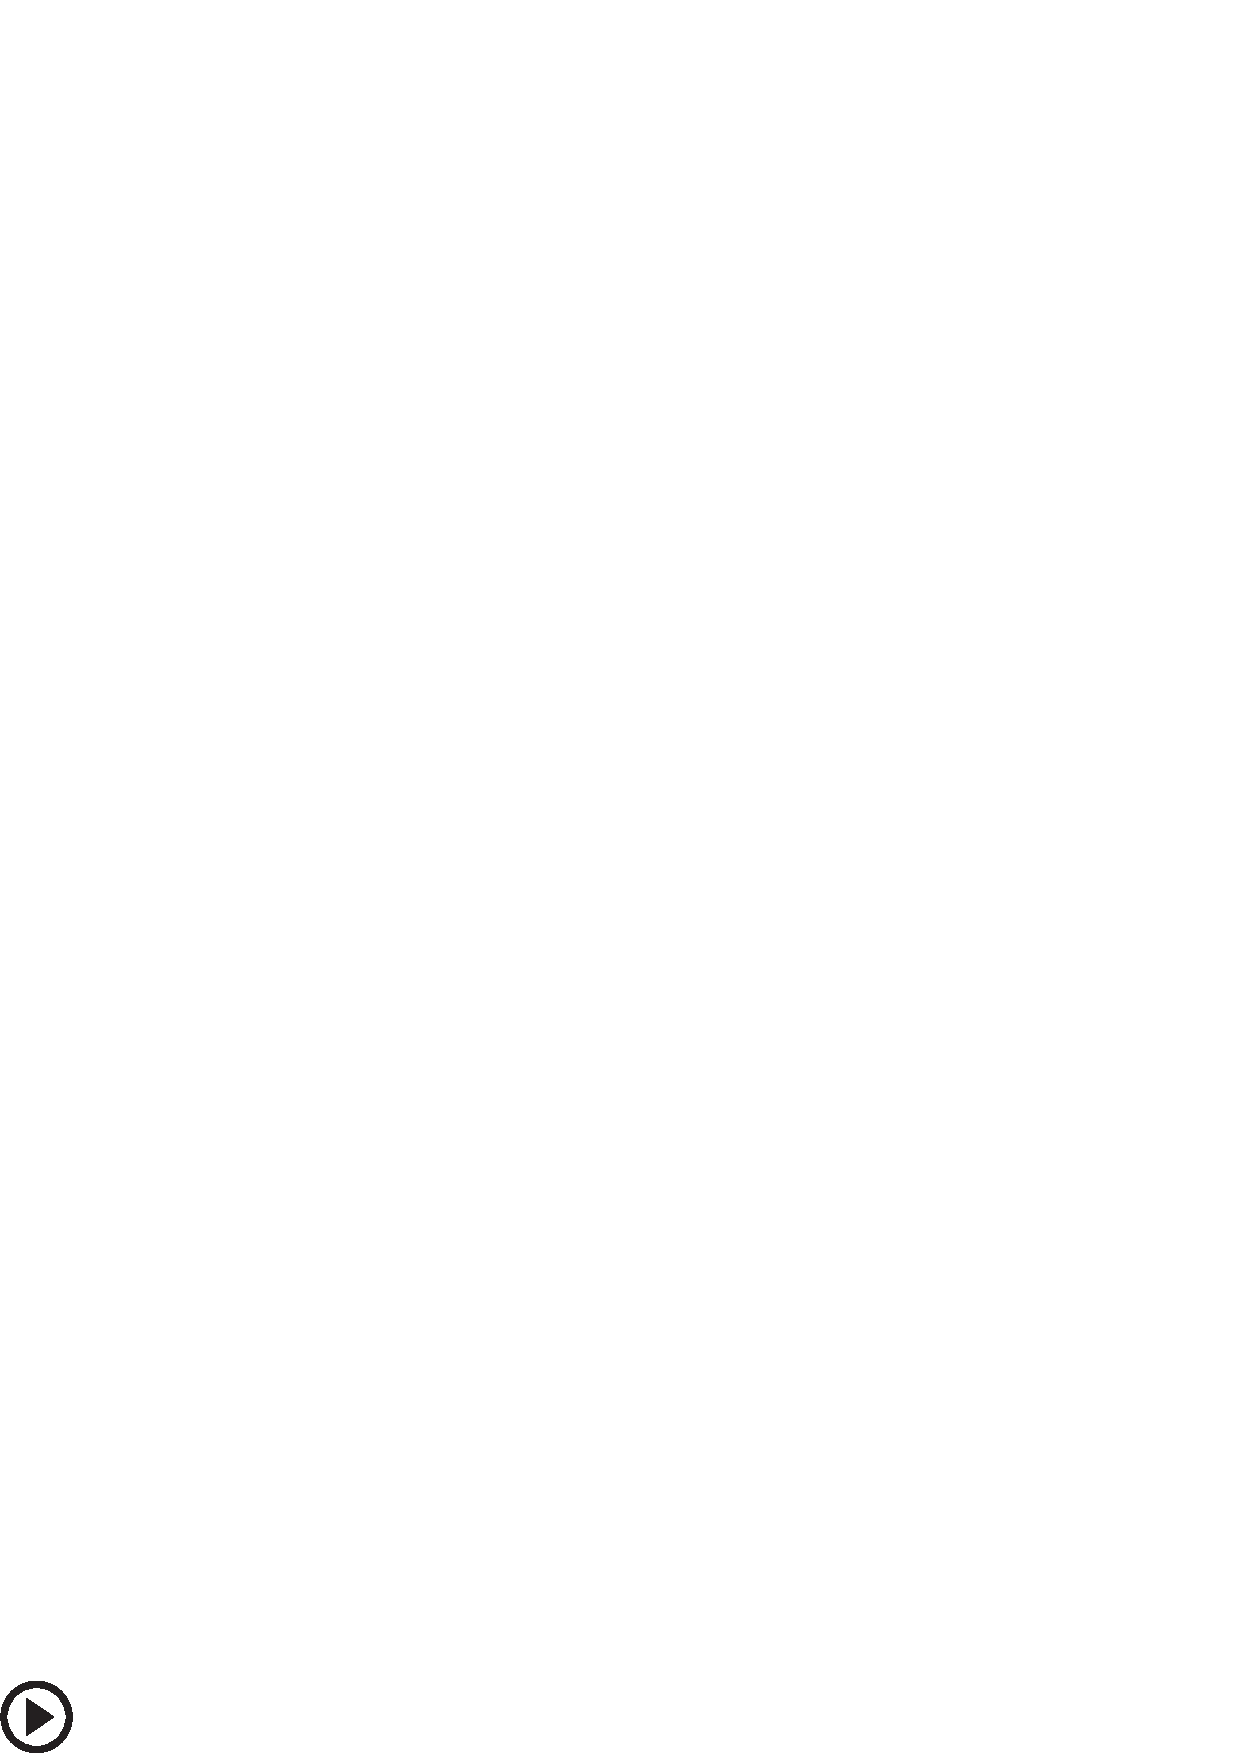
\includegraphics[height=1em]{../../icons/video.pdf}} VMiwd by www.everythingmaths.co.za



}





% Webbook page

\newpage
\thispagestyle{empty}

{\normalfont\sffamily\fontsize{22}\normalfont\itshape Meer as net 'n handboek} \par

\begin{center}
\includegraphics[width=0.70\textwidth]{../title_images/morethantextbookAfrikaans.png}
\end{center}

\par
{\Large
\textbf{\textit{Everything Maths}} is not just a Maths textbook. It has everything you expect from
your regular printed school textbook, but comes with a whole lot more. For a start, your learners can download or read it
online on their mobile phone, computer or iPad, which means you have the convenience of accessing
it wherever you are.\par


It is good for learners to hear and read different explanations of concepts as it affords them a more well-rounded understanding of the work. This is why every chapter comes with links to online video
lessons and explanations, which help bring the ideas and concepts to life. Summary presentations at
the end of every chapter offer an overview of the content covered, with key points highlighted for easy
revision.\par

All the exercises inside the book link to an on-line service where
learners can get more practice, see the full
solutions or test their skills level on mobile and PC. Every educator knows that the key to success in maths is practice, practice, practice!
\par


We are interested to know what you as an educator think about our books, as well as what the learners
wonder about or struggle with as they make their way through the content and attempt the exercises. That is
why we have made it possible for educators and learners to use their mobile phones or computers to access
the books on-line and digitally pin a question to a page and see what questions and answers other readers
pinned up too.
\par


% This book is the same one used by Mindset Learn in their new television broadcast, where experienced educators work through it, explain the concepts and work out exercises from the book.
}




% mobile or PC
\newpage
\thispagestyle{empty}

{\normalfont\sffamily\fontsize{22}\normalfont\itshape Lees dit op jou selfoon of rekenaar} \par

{\Large
Learners can have this textbook at hand wherever they are – whether at home, on the the train or at school.
They can browse the on-line version of Everything Science on their mobile phone, tablet or computer. To
read it off-line, a PDF or e-book version can be downloaded. Learners can also access Everything Maths
and Everything Science for not only Grade 10, but also for Grades 11 and 12 on their mobile phone! There is
now no excuse for a learner to not have these textbooks in front of them in class!
\par


To read or download the textbook on their phone or computer, direct learners to \\ \underline{www.everythingmaths.co.za}} \vspace*{2cm}


\begin{center}
\begin{minipage}{0.4\textwidth}
\centering
\includegraphics[width=1\textwidth]{../title_images/ipad.jpg}
\end{minipage}
\begin{minipage}{0.4\textwidth}
\centering
\includegraphics[width=0.4\textwidth]{../title_images/phone.png}
\end{minipage}
\end{center}

\vspace*{2cm}


{\normalfont\sffamily\fontsize{22}\normalfont\itshape Links to support materials} \par

{\Large
Inside the book you will find these icons to help you and your learners spot where online videos, presentations, practice tools
and more help exist. The short-codes next to the icons allow you to navigate directly to the resources
on-line without having to search for them. Visit \underline{www.everythingmaths.co.za} and enter the short-codes in the navigation box.\par


\begin{tabular}{lcl}
\raisebox{-0.8em}{\includegraphics[width=0.8cm]{../../icons/www.pdf}} & (A123) & Gaan direk na 'n afdeling\\
\raisebox{-0.8em}{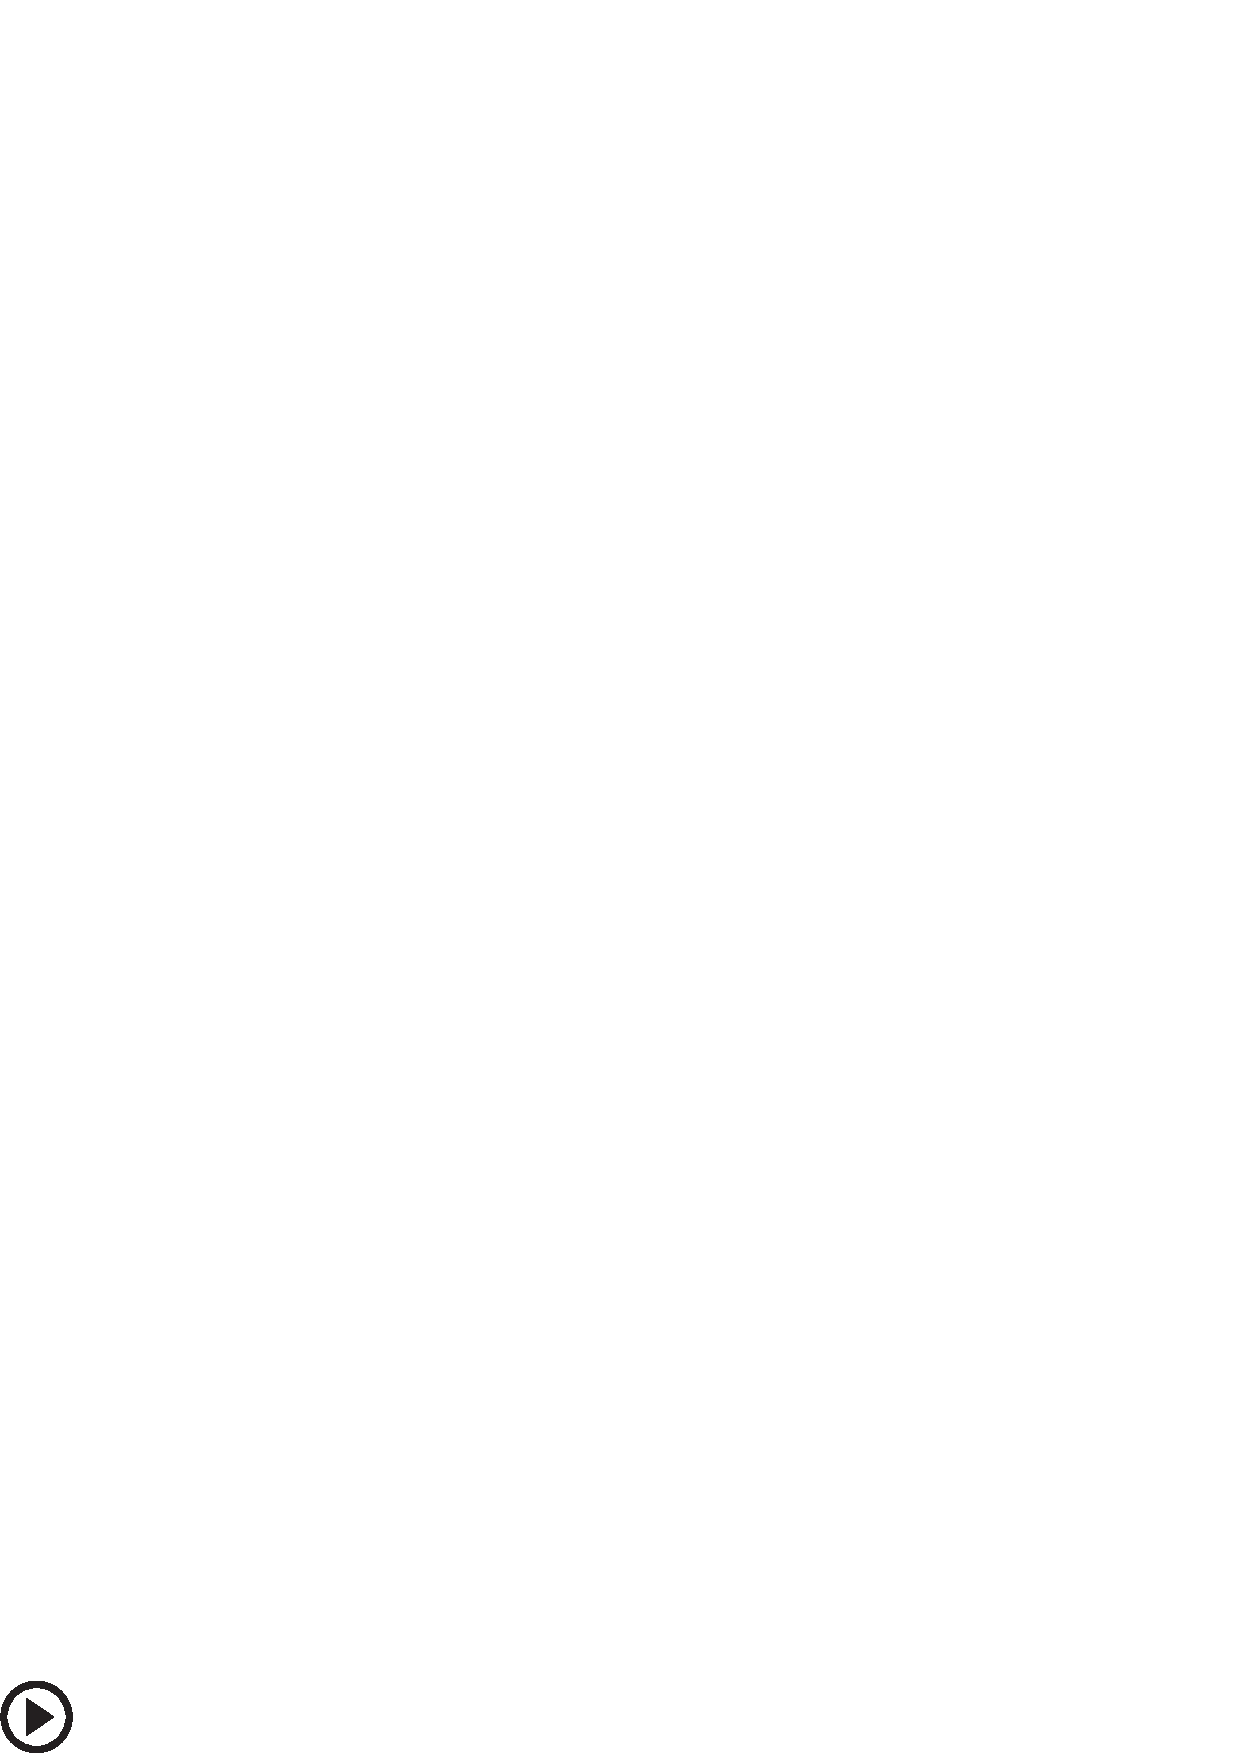
\includegraphics[width=0.8cm]{../../icons/video.pdf}} & (V123) & Video, simulasie of aanbieding \\
\raisebox{-0.8em}{\includegraphics[width=0.8cm]{../../icons/aplus.pdf}} & (P123) & Oefen en toets jou vaardighede \\
\raisebox{-0.8em}{\includegraphics[width=0.8cm]{../../icons/help.pdf}} & (Q123) & Vra vir hulp of vind 'n antwoord \\
\end{tabular}
\par
\vspace*{1cm}

% To watch the videos on-line, practise your skills or post a question, go to the \textit{Everything Maths} website at \underline{www.everythingmaths.co.za} on your mobile or PC and enter the short-code in the navigation box.
}




% video lessons
\newpage
\thispagestyle{empty}

{\normalfont\sffamily\fontsize{22}\normalfont\itshape Video-lesse} \par

{\Large

Look out for the video icons inside the book. These will take you to online video lessons created by Mindset
Learn and the Khan Academy that help bring the ideas and concepts on the page to life. Learners can now get extra insight, detailed
explanations and worked examples, while also seeing the concepts in action and hearing real people talk about how they use maths and science in their work!  \par

This is a great way for you to bring technology into your classroom – using a projector or digital whiteboard, access the books on \underline{www.everythingmaths.co.za} and use the videos to provide an additional summary of the concepts you have covered by offering an alternative explanation. After hours, learners that need additional help will know that they can watch the videos in their own time, with the added bonus of being able to stop, pause and rewind the explanation until they have fully grasped the concept. This is great for revision purposes too, as it is like having a personal teacher on hand for every learner, at any time! \par
\begin{figure}[h]
\begin{center}
Sien video verduideliking \raisebox{-0.6em}{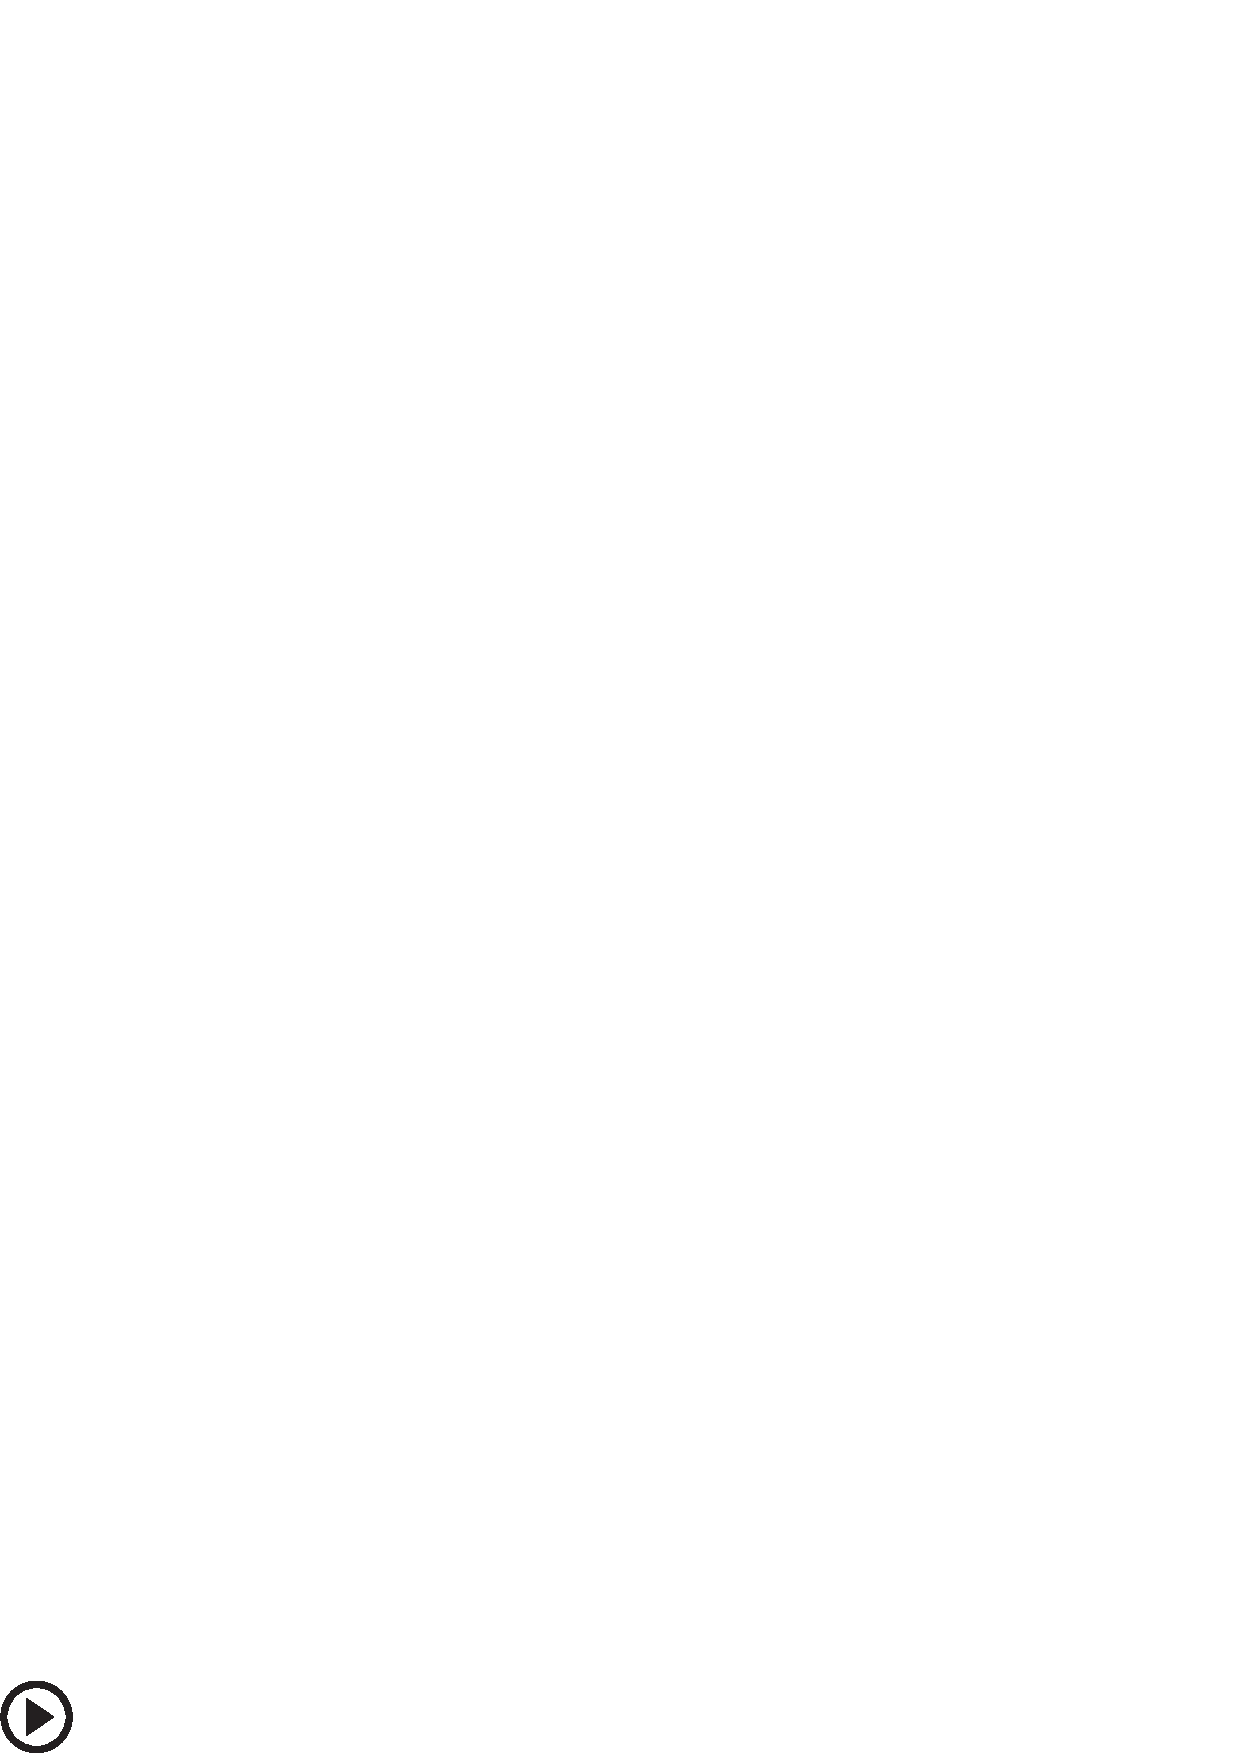
\includegraphics[width=0.7cm]{../../icons/video.pdf}} (Video: V123)\\
\includegraphics[width=0.5\textwidth]{../title_images/veritasiumvideo.png}
\end{center}
\end{figure}

}


\vspace{0.5cm}
{\normalfont\sffamily\fontsize{22}\normalfont\itshape Video oefeninge} \par

{\Large
As daar oefeninge in die boek is, sal jy die ikons en kortkodes vir video-oplossings, oefeninge en hulp sien. 

 By entering these short-codes into the box on our website, learners will be taken to video solutions of select exercises to show them
step-by-step how to solve such problems. Encourage your learners to access these video exercises, which are great for revision purposes as well as to reinforce your own teaching.\par

\begin{figure}[h]
\begin{center}
Sien video oefening \raisebox{-0.6em}{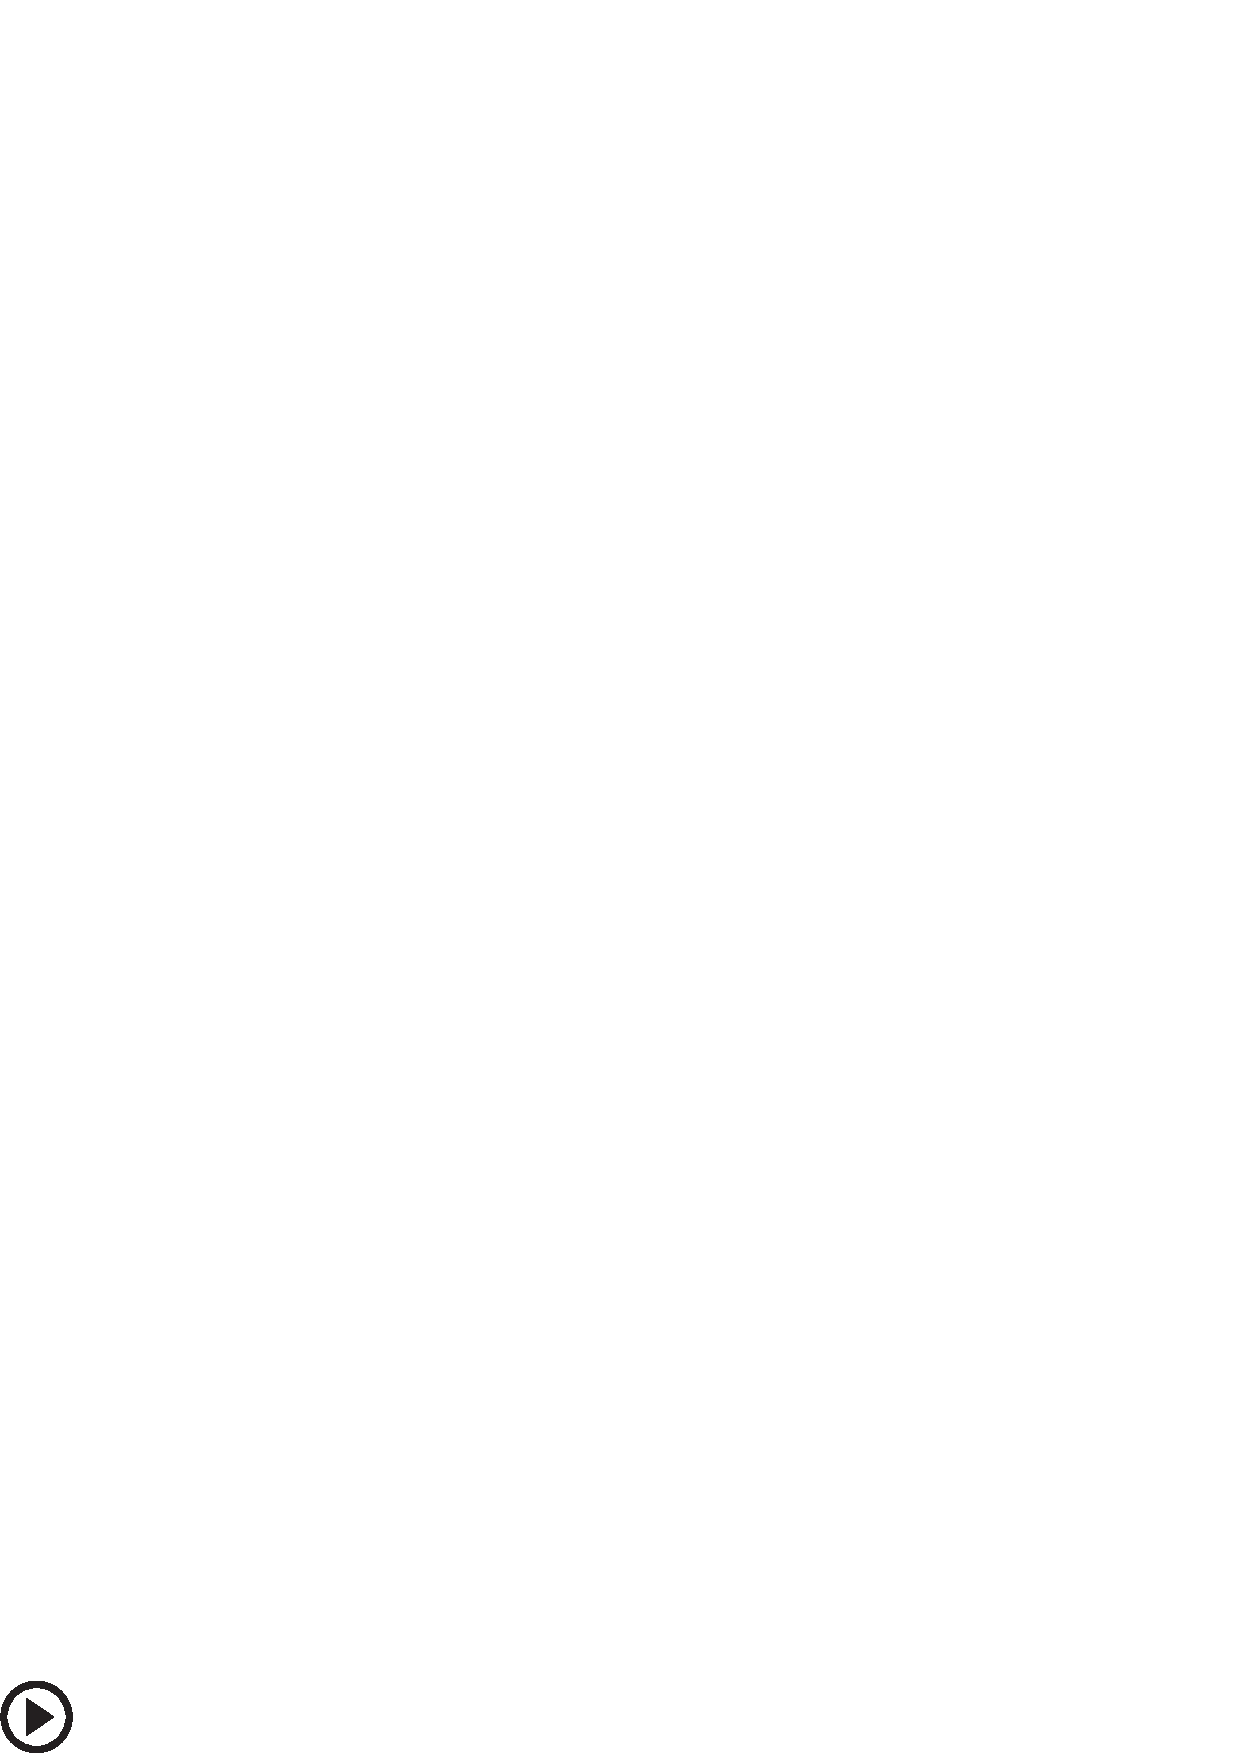
\includegraphics[width=0.7cm]{../../icons/video.pdf}} (Video: V123)\\ 
\includegraphics[width=0.5\textwidth]{../title_images/mindsetexercise.png}
\end{center}
\end{figure}

Jy kan toegang tot die videos kry deur:
\begin{itemize}[noitemsep]
\item hulle aanlyn op jou selfoon of rekenaar te kyk
\item die videos af te laai sodat jy die van lyn af op jou selfoon of rekenaar kan kyk.
\item ‘n DVD te bestel wat jy op jou TV of rekenaar kan speel.
\item dit van lyn af af te laai met Bluetooth of Wi-Fi van sekere afsetpunte
\end{itemize}
For additional viewing, downloads or more information, visit the \textit{Everything Maths} website on your phone or computer at \underline{www.everythingmaths.co.za}.


Om nog videos te sien, of vir meer inligting, besoek die Everything Maths webblad vanaf jou selfoon of rekenaar by \underline{www.everythingmaths.co.za}    \par
\vspace*{1cm}
}


% monassis
% \newpage
% \thispagestyle{empty}

{\normalfont\sffamily\fontsize{22}\normalfont\itshape Setting tests with Monassis} \par

{\Large
Siyavula offers an open online assessment bank called Monassis, for the sharing and accessing of
curriculum-aligned test and exam questions with answers. All the questions and solutions found in the
textbook are hosted on-line on Monassis. In addition to this, this site enables educators to quickly set tests
and exam papers, by selecting items from the library and adding them to their test. Educators can then
download their separate test and memo which is ready for printing. Monassis further offers educators the
option of capturing their learners' marks in order to view a selection of diagnostic reports on their
performance.
\begin{figure}[H]
\begin{center}
\raisebox{-0.6em}{

\includegraphics[width=0.5\textwidth]{../title_images/monassis.png}}
\end{center}
\end{figure}



% \begin{figure}[H]
%  \begin{center}
% \raisebox{-0.6em}{
% \includegraphics[width=0.5\textwidth]{monassis.png}}
% \end{center}
% \end{figure}

We encourage you to make use of Monassis - let it help you save time setting tests and analysing learner marks! For further information visit \underline{www.monassis.com}.






% {\normalfont\sffamily\fontsize{16}\normalfont\itshape  How do I do Each of These?}\par 
% \textbf{Share and access questions}\par 
% Sharing questions: use either the online editor or OpenOffice template which can be downloaded from the website (Browse questions → Contribute questions → Import questions). Take your test/worksheet/other question source. Break it up into the smallest sized individual questions that make sense, and use the template style guide to style your page according to question/answer. Upload these questions or type them up in the online editor (Browse questions → Contribute questions → Add questions). Do not include overall question numbering but do include sub numbering if needed (e.g. 1a, 2c, etc.). Insert the mark and time allocation, tag questions according to grade, subject i.e. a description of the question, and then select the topics from the topic tree. Finalise questions so that they can be used in tests and accessed by other Monassis users.\par 
% 
% Accessing questions: there are three ways to access questions in the database. Click on “Browse questions” → click on the arrow to the left of the grade, which opens out the subjects → keep clicking on the arrows to open the learning outcomes or, following the same process, instead of clicking on the arrow, click on the grade → now you can browse the full database of questions for all the subjects in that grade or, from the landing page, click on “Browse questions” → below the banner image click on “Find Questions” → search by topics, author (if you know a contributor), text or keywords e.g. Gr10 mathematics functions and graphs. \par 
% 
% \textbf{Create tests from questions
% }\par 
% So, you have all these bits of tests (i.e. many questions!), but what you really want is the actual test. How do you do this? Well, you can simply click “add to test” on any question and then click on the “Tests” tab at the top right of the page, and follow the simple instructions. Alternatively you can create a test by starting with clicking on that same “Tests” tab, and add questions to your test that way. Once done, simply print off the PDF or Word file of the questions, issue your test, collect them once complete, and mark them using the memo provided by Monassis. \par 
% 
% \textbf{Create class lists}\par 
% 
% But now you are asking, how can I keep track of my classes? Is Johnny Brown in class A or B? Well, you can make a class list by clicking on the “Class lists” tab at the top right of the page, and either import a CSV file, or manually enter the relevant information for each class. Now you can issue tests  to your classes, and have a class list for each class. And what about capturing their marks?\par 
% 
% \textbf{Create scoresheets}\par 
% For each test you can create a scoresheet. Select the “Tests” tab at the top right, click on “Marks” below the banner image, and select the test and follow the instructions to input their marks. You can then export these as a CSV file for use in spreadsheets.\par 
% 
% \textbf{Analyse learners' performance}\par 
% 
% And finally, you can print out reports of class performance. Click on “Reports” at the top right of the page, which opens various reports you can view. There are reports to see class performance, learner performance, class performance per topic, class performance per question, learner strengths and weaknesses, and learner progress.\par 
% So now you know how Monassis works, we encourage you to make use of its simple functionality, and let it help you save time setting tests and analysing learner marks!\par 
% 
}





% practise and test your skills
\newpage
\thispagestyle{empty}
{\Large


{\normalfont\sffamily\fontsize{22}\normalfont\itshape Intelligent practice for learners} \par

One of the best ways for learners to prepare for tests and exams is to practice answering the same kind of questions they will be tested on. At every set of exercises you will see a practice icon and short-code, which link to an online database for learners to practice further exercises. Point your learners at \underline{www.everythingmaths.co.za} on their mobile phone or PC. where they can enter the short-code from the textbook into the box on the website, and be redirected to additional exercises online. This on-line practice on mobile and PC will keep track of learners' performance and progress, give them feedback on areas which require more attention, and suggest which sections or videos to look at.\par
\begin{figure}[H]
\begin{center}
See more practice \raisebox{-0.6em}{\includegraphics[width=0.7cm]{../../icons/aplus.pdf}} (QM123)\\ 
\includegraphics[width=0.65\textwidth]{../title_images/practicephones.png}
\end{center}
\end{figure}
\par
The software can generate any number of questions with the same structure but different details i.e. the numerical values in physics or maths problems can change each time, but the type of question can stay the same. This allows much more variety than a traditional question bank - to the extent that a different practice test can be created automatically for each student in a class. The system also generates a memorandum along with each test, and tracks the learners' conceptual understanding through their success at answering different types of questions.\par

This tool aims to discover the strong and weak points in learners' understanding as the learners are going through worked examples and drilling exam problems. By knowing with which concepts learners are struggling, the system can then do useful things like
\begin{itemize}[noitemsep]
\item provide more practice on the types of questions with which the learner is struggling;
\item recommend revision material from freely available educational resources (for example,  Siyavula's \textit{Everything Maths} and \textit{Everything Science} textbooks);
\item provide feedback and reports to learners, educators and parents about their progress and about the specific concepts to which they should pay more attention.
\end{itemize}
 The above is done for each learner individually, delivering a customised practice and revision schedule to match his or her pace and understanding.





% For learners to practice and test their skills, point them at \underline{www.everythingmaths.co.za} on their mobile phone or PC and enter the short-code in the box.\par

\vspace*{1cm}
}
\\
{\normalfont\sffamily\fontsize{22}\normalfont\itshape Helping learners find answers} \par

{\Large
If a learner is stuck on a particular section of work in the textbook, they can get additional help by visiting \underline{www.everythingmaths.co.za} on their phone or computer, and find out if other learners also had a question about that same section of the work. If a question has been posted, educators can go on-line and respond, thereby helping other learners that may have been stuck on the same problem. \par




\begin{tabular}{lcl}
\raisebox{-0.8em}{\includegraphics[width=0.8cm]{../../icons/www.pdf}} & (P78) & Visit this section to post or view questions \\

\raisebox{-0.8em}{\includegraphics[width=0.8cm]{../../icons/help.pdf}} & (QM123) & Ask for help or find an answer \\
\end{tabular}
\par
\vspace*{1cm}

\begin{figure}[H]
\centering
\includegraphics[width=\textwidth]{../title_images/questions.png}
\end{figure}

Using the short-codes at section headings and exercises in the textbook, learners can go to the above website, enter the short-code into the box on-line, and be redirected to the relevant place in the book. Once there they can pin their question at the exact spot where it cropped up (see image below), by highlighting a specific section of the text. They will be able to see whether the question has been asked before by other learners, and what the given answer to that question is. \par
% Look out for these icons in the texbook: \par
% Visit the Everything Maths website on your phone or computer at \underline{www.everythingmaths.co.za }\par
}
\pagebreak
{\normalfont\sffamily\fontsize{22}\normalfont\itshape Tell us how to improve the book} \par

{\Large
If you have any comments, thoughts or suggestions on the books, visit \underline{www.everythingmaths.co.za}, and
switch to educator mode (you will see on the website how to do this), and using our annotator tool, you can
capture these in the text. These can range from sharing tips and ideas on the content in the textbook with
your fellow educators, to discussing how to better explain concepts in class. Also, if you have picked up any
errors in the book you can make a note of them here, and we will correct them in time for the next print run.
The image below illustrates this.
 \par


\begin{figure}[H]
\centering
\includegraphics[width=\textwidth]{../title_images/annotater.png}
\end{figure}

Using the short-codes at section headings and exercises in the textbook, learners can go to the above website, enter the short-code into the box on-line, and be redirected to the relevant place in the book. Once there they can pin their question at the exact spot where it cropped up (see image below), by highlighting a specific section of the text. They will be able to see whether the question has been asked before by other learners, and what the given answer to that question is. \par
% Look out for these icons in the texbook: \par
% Visit the Everything Maths website on your phone or computer at \underline{www.everythingmaths.co.za }\par
}
% %television
% \newpage
% \thispagestyle{empty}
% {\normalfont\sffamily\fontsize{22}\normalfont\itshape Television broadcasts} \par
% This book is the same one used by \textbf{Mindset Learn} in their television broadcast where experienced
% educators explain the key concepts, perform live experiments and work out exercises from the book.
% \textbf{Mindset Learn} broadcasts a full 28 hours of curriculum support each week of term. \par
% 
% 
% Maths can be seen on Mondays and Science on Tuesdays. There is also Life Sciences on Wednesdays
% and Maths Literacy on Thursdays. Revision of the week's work is done on Saturdays for Grade 12 and on
% Sundays for Grades 10 and 11.
% 
% 
% }
%ask questions, find answers
% \newpage
% \thispagestyle{empty}


% 
% 
% 
% 
% {\Large
% 
% \begin{table*}[h]
% \large
% \begin{tabular}{lll}
% \textbf{Maths and Science Broadcasts}&&\\
% Grade 10  Maths & Mondays at 4pm & Every second Sunday at 1pm\\
% Grade 11  Maths & Mondays at 5pm & Every second Sunday at 9am\\
% Grade 12  Maths & Mondays at 6pm & Every Saturday at 9am\\
% Grade 10  Science & Tuesdays at 4pm & Every second Sunday at 1pm\\
% Grade 11  Science & Tuesdays at 5pm & Every second Sunday at 9am\\
% Grade 12  Science & Tuesdays at 6pm & Every Saturday at 11am\\
% \textbf{Other broadcasts} & & \\
% Grade 10  Life Science & Wednesdays at 4pm & Every second Sunday at 3pm\\
% Grade 11  Life Science & Wednesdays at 5pm & Every second Sunday at 9am\\
% Grade 12  Life Science & Wednesdays at 6pm & Every Saturday at 1pm\\
% Grade 10  Maths Literacy & Thursdays at 4pm & Every second Sunday at 3pm\\
% Grade 11  Maths Literacy & Thursdays at 5pm & Every second Sunday at 9am\\
% Grade 12  Maths Literacy & Thursdays at 6pm & Every Saturday at 3pm\\
% \end{tabular}
% \end{table*}
% 
% \\
% \textbf{You can watch these live sessions on:}
% \begin{itemize}
%     \item Mindset free-to-air for schools (ask your school)
%     \item Channel 319 on DStv
%     \item TopTV on 319 
% \end{itemize}
% 
% 
% }








% Put the margins back for the rest of the book

\newgeometry{lmargin=0.1\paperwidth, rmargin=0.25\paperwidth, tmargin=1in, bmargin=1in, twoside, centering, includehead,  marginparwidth=0.225\paperwidth}

\normalfont
 

\tableofcontents
\mainmatter

\renewcommand{\sectionmark}[1]{\markright{\thesection}{}}
\renewcommand{\footrulewidth}{0.4pt}

\newpage


% chapter includes


%     \chapter{Algebraic Expressions}
    \fancyfoot[LO,RE]{Focus Area: Mathematics}
    \section{Rational and Irrational Numbers}
    \setcounter{figure}{1}
    \setcounter{subfigure}{1}
    \label{m38348}
            \nopagebreak
            \label{m38348*cid2} $ \hspace{-5pt}\begin{array}{cccccccccccc}   \includegraphics[width=0.75cm]{col11306.imgs/summary_video.png} &   \end{array} $ \hspace{2 pt}\raisebox{-5 pt}{} {(subsection shortcode: MG10033 )} \par 
      \label{m38348*id62184}A number is a way of representing quantity. The numbers that will be used in high school are all real numbers, but there are many different ways of writing any single real number.\par 
      \label{m38348*id62191}This section describes \textsl{rational numbers}.\par \label{m38348*eip-195}
    \setcounter{subfigure}{0}
	\begin{figure}[H] % horizontal\label{m38348*circuits-1}
    \textnormal{Khan Academy video on Integers and Rational Numbers}\vspace{.1in} \nopagebreak
  \label{m38348*yt-media1}\label{m38348*yt-video1}
            \raisebox{-5 pt}{ \includegraphics[width=0.5cm]{col11306.imgs/summary_www.png}} { (Video:  MG10034 )}
      \vspace{2pt}
    \vspace{.1in}
 \end{figure}       

\par 
    \subsection*{The big picture of numbers}
    \addcontentsline{toc}{subsection}{The big picture of numbers}

            \label{m38348*cid3} $ \hspace{-5pt}\begin{array}{cccccccccccc}   \end{array} $ \hspace{2 pt}\raisebox{-5 pt}{\includegraphics[width=0.5cm]{col11306.imgs/summary_www.png}} {(subsection shortcode: MG10035 )} \par 
      \label{m38348*id62547}
    \setcounter{subfigure}{0}
	\begin{figure}[H] % horizontal\label{m38348*id62548}
    \begin{center}
    \label{m38348*id62548!!!underscore!!!media}\label{m38348*id62548!!!underscore!!!printimage}
%\includegraphics[width=9cm]{col11306.imgs/m38348_MG10C3_001.png} % m38348;MG10C3\_001.png;;;6.0;8.5;
\scalebox{0.6} % Change this value to rescale the drawing.
{
\begin{pspicture}(0,-4.764375)(14.481563,4.804375)
\psellipse[linewidth=0.04,dimen=outer](6.81,-0.484375)(6.81,4.28)
\psline[linewidth=0.04cm](8.18,3.695625)(8.26,-4.684375)
\psellipse[linewidth=0.04,dimen=outer](4.34,-1.364375)(3.8,2.5)
\psellipse[linewidth=0.04,dimen=outer](3.57,-1.854375)(2.57,1.61)
\usefont{T1}{ppl}{b}{n}
\rput(6.735781,4.350625){\Huge REAL $\mathbb{R}$}
\usefont{T1}{ppl}{b}{n}
\rput(11.03875,-0.484375){\Large Irrational $\mathbb{Q'}$}
\usefont{T1}{ppl}{b}{n}
\rput(5.11875,1.975625){\Large Rational $\mathbb{Q}$}
\usefont{T1}{ppl}{b}{n}
\rput(4.06875,0.275625){\Large Integers $\mathbb{Z}$}
\usefont{T1}{ppl}{b}{n}
\rput(3.21875,-2.324375){\Large Natural $\mathbb{N}$}
\psellipse[linewidth=0.04,dimen=outer](3.14,-2.354375)(1.68,0.83)
\usefont{T1}{ptm}{b}{n}
\rput(3.5735939,-1.024375){\Large Whole $\mathbb{N}_0$}
\end{pspicture} 
}
      \vspace{2pt}
    \vspace{.1in}
    \end{center}
 \end{figure}       
      \par 
      We use the following definitions:\par 
      \label{m38348*id62559}\begin{itemize}[itemsep=5pt]
            \label{m38348*uid1}\item natural numbers are $\{1, 2, 3, ...\}$
\label{m38348*uid2}\item whole numbers are $\{0, 1, 2, 3, ...\}$
\label{m38348*uid3}\item integers are $\{... -3, -2, -1, 0, 1, 2, 3, ....\}$
\end{itemize}

            \nopagebreak
            \label{m38348*cid4} $ \hspace{-5pt}\begin{array}{cccccccccccc}   \end{array} $ \hspace{2 pt}\raisebox{-5 pt}{\includegraphics[width=0.5cm]{col11306.imgs/summary_www.png}} {(subsection shortcode: MG10036 )} \par 
  
\Definition{Rational number}{
      \label{m38348*id62709}A rational number is any number which can be written as: 
%       \label{m38348*uid6}\nopagebreak\noindent{}
        
    \begin{equation}
    \frac{a}{b}
      \end{equation}
      \label{m38348*id62732}where $a$ and $b$ are integers and $b\ne 0$. \par 
       } 


    \label{m38348*id62607}The following numbers are all rational numbers.\par 
      \label{m38348*uid4}\nopagebreak\noindent{}
        
    \begin{equation}
    \frac{10}{1},\frac{21}{7},\frac{-1}{-3},\frac{10}{20},\frac{-3}{6}
      \end{equation}
      \label{m38348*id62687}You can see that all denominators and all numerators are integers.\par 
% \label{m38348*fhsst!!!underscore!!!id138}\begin{definition}
% 	  \begin{tabular*}{15 cm}{m{15 mm}m{}}
% 	\hspace*{-50pt}  \includegraphics[width=0.5in]{col11306.imgs/psflag2.png}   & 



%       \end{tabular*}
%       \end{definition}
% \label{m38348*eip-761}Note that because we can write $\dfrac{a}{-b}$
% as $\dfrac{-a}{b}$
% (in other words, one can always find an equivalent rational expression where $b\greatthan{}0$) mathematicians typically define rational numbers not as both $a$ and $b$ being integers, but rather that $a$ is an integer and $b$ is a natural number. This avoids having to worry about zero in the denominator. \par \label{m38348*notfhsst!!!underscore!!!id150}
% % \begin{tabular}{cc}
% % 	   \hspace*{-50pt}\raisebox{-8 mm}{ \includegraphics[width=0.5in]{col11306.imgs/pstip2.png}  }& 
% 	\begin{minipage}{0.85\textwidth}
% 	
%       \Tip{Only fractions which have a numerator and a denominator (that is not 0) that are integers
% are rational numbers.}
% % 	\end{note}
% 	\end{minipage}
% % 	\end{tabular}
	\par
      \label{m38348*id62778}This means that all integers are rational numbers, because they can be written with a denominator of 1.\par 
      \label{m38348*id62782}Therefore\par 
      \label{m38348*uid7}\nopagebreak\noindent{}
        
    \begin{equation}
    \frac{\sqrt{2}}{7} ; \frac{20}{\pi}
      \end{equation}
      \label{m38348*id62817}are \textbf{not examples} of rational numbers, because either the numerator or the denominator is not an integer.\par 
      \label{m38348*id62829}A number may not be written as an integer divided by another integer, but may still
be a rational number. The rule is, if a number \textbf{can be} written
as a fraction of integers, it is rational even if it can be written in other
ways as well. Here are two examples that might not look like rational numbers
at first glance, but are because there are equivalent forms that are expressed as an
integer divided by another integer:\par 
      \label{m38348*uid8}\nopagebreak\noindent{}
    \begin{equation}    
    \frac{-1,33}{-3}=\frac{133}{300}; ~~~~~~\frac{-3}{6,39}=\frac{-300}{639}=\frac{-100}{213}
      \end{equation}
\label{m38348*secfhsst!!!underscore!!!id232}
% begin{exercise}   \subsubsubsection

     


    \subsection*{Decimal numbers}
    \addcontentsline{toc}{subsection}{Decimal numbers}
            \nopagebreak
            \label{m38348*cid5} $ \hspace{-5pt}\begin{array}{cccccccccccc}   \end{array} $ \hspace{2 pt}\raisebox{-5 pt}{\includegraphics[width=0.5cm]{col11306.imgs/summary_www.png}} {(subsection shortcode: MG10037 )} \par 
      \label{m38348*id63345}All integers and fractions with integer numerators and denominators are rational numbers. There are two more forms of rational numbers.\par 
\label{m38348*secfhsst!!!underscore!!!id245}



\begin{Investigation}{Decimal Numbers }
            \nopagebreak
      \label{m38348*id63357}You can write the rational number
$\frac{1}{2}$ as the decimal number 0,5. Write the following numbers as
decimals and investigate them:\par 
      \label{m38348*id63375}\begin{enumerate}[itemsep=5pt, label=\textbf{\arabic*}. ] 
            \label{m38348*uid11}\item 
          $\dfrac{1}{4}$
        \label{m38348*uid12}\item 
          $\dfrac{1}{10}$
        \label{m38348*uid13}\item 
          $\dfrac{2}{5}$
        \label{m38348*uid14}\item 
          $\dfrac{1}{100}$
        \label{m38348*uid15}\item 
          $\dfrac{2}{3}$
        \end{enumerate}
      \label{m38348*id63486}Do the numbers after the decimal comma end or do they continue? If they continue, is there a recurring pattern to the numbers? \par 
\end{Investigation}
      \label{m38348*id63495}You can write any rational number as a decimal number but not all decimal numbers are rational numbers. However, two types of decimal numbers can be written as rational numbers:\par 
      \label{m38348*id63500}\begin{enumerate}[itemsep=5pt, label=\textbf{\arabic*}. ] 
            \label{m38348*uid16}\item decimal numbers that end or \textsl{terminate}, for example the fraction $\dfrac{4}{10}$ can be written as $0,4$.
\label{m38348*uid17}\item decimal numbers that have a recurring pattern of numbers, for example the fraction $\dfrac{1}{3}$ can be written as 
$0,\dot{3}$. 
The dot represents recurring $3$'s i.e.,
$0,333...=0,\dot{3}$.
\end{enumerate}
      \label{m38348*id63576}The rational number $\dfrac{5}{6}$ can be written in decimal notation as $0,8\dot{3}$ and similarly, the decimal number 0,25 can be written as a rational number as $\dfrac{1}{4}$.\par 
\label{m38348*notfhsst!!!underscore!!!id301}
% \begin{tabular}{cc}
% 	   \hspace*{-50pt}\raisebox{-8 mm}{ \includegraphics[width=0.5in]{col11306.imgs/pstip2.png}  }& 
% 	\begin{minipage}{0.85\textwidth}
% 	\begin{note}
      \Tip{You can use a dot or a bar over the repeated numbers to indicate that the decimal is a recurring decimal.}
% 	\end{note}
% 	\end{minipage}
% 	\end{tabular}
	\par

    \subsection*{Converting terminating decimals into rational numbers}
    \addcontentsline{toc}{subsection}{Converting terminating decimals into rational numbers}
%             \nopagebreak
%             \label{m38348*cid6} $ \hspace{-5pt}\begin{array}{cccccccccccc}   \end{array} $ \hspace{2 pt}\raisebox{-5 pt}{\includegraphics[width=0.5cm]{col11306.imgs/summary_www.png}} {(subsection shortcode: MG10038 )} \par 
%       \label{m38348*id63646}A decimal number has an integer part and a fractional part. For example $10,589$ has an integer part of 10 and a fractional part of $0,589$ because $10+0,589=10,589$. The fractional part can be written as a rational number, i.e. with a numerator and a denominator that are integers.\par 
%       \label{m38348*id63704}Each digit after the decimal point is a fraction with a denominator in increasing powers of ten. For example:\par 
% 
% 
%       \label{m38348*id63708}\begin{itemize}[itemsep=5pt]
%             \label{m38348*uid18}\item $\dfrac{1}{10}$ is $0,1$\label{m38348*uid19}\item $\dfrac{1}{100}$ is $0,01$\end{itemize}
%       \label{m38348*id63781}This means that:\par 
%       \label{m38348*id63784}\nopagebreak\noindent{}
%     \begin{equation}
%    \hfill 10,589& =& 10+\frac{5}{10}+\frac{8}{100}+\frac{9}{1000}\hfill \\ & =& 10\frac{589}{1000}\hfill \\ & =& \frac{10589}{1000}\hfill 
%       \end{equation}
% \label{m38348*secfhsst!!!underscore!!!id378}
% 
% 

% 
% 
%     \subsection{ Converting Repeating Decimals into Rational Numbers}
            \nopagebreak
            \label{m38348*cid7} $ \hspace{-5pt}\begin{array}{cccccccccccc}   \end{array} $ \hspace{2 pt}\raisebox{-5 pt}{\includegraphics[width=0.5cm]{col11306.imgs/summary_www.png}} {(subsection shortcode: MG10039 )} \par 


      \label{m38348*id63993}When the decimal is a recurring decimal, a bit more work is needed to write the fractional part of the decimal number as a fraction.\par 
      
\begin{wex}
{%title
Converting decimal numbers to fractions
}
{%question
\\
Write $0,\dot{3}$ in the form $\dfrac{a}{b}$ (where $a$ and $b$ are integers)
}
{%answer

\westep{}
$$x = 0,33333\ldots$$


\westep{Multiply by 10 on both sides}

$$10x = 3,33333\ldots$$


\westep{Subtract the second equation from the first equation}

$$9x = 3 $$

\westep{Simplify}

$$ x = \dfrac{3}{9} = \dfrac{1}{3} $$
}
\end{wex}


\begin{wex}
{%title
Converting decimal numbers to fractions
}
{%question
\\Write $5,\dot{4}\dot{3}\dot{2}$ as a rational fraction
}
{%answer

\westep{}

$$ x = 5,432432432\ldots $$

\westep{Multiply by 1000 on both sides}

$$ 1000x = 5432,432432432\ldots $$

\westep{Subtract the second equation from the first}

$$ 999x = 5427 $$

\westep{Simplify}

$$ x = \dfrac{5427}{999} = \dfrac{201}{37} $$
 
}
\end{wex}





%       \label{m38348*id64237}And another example would be to write 
% $5,\dot{4}\dot{3}\dot{2}$ 
% as a rational fraction.
% \par 
%       \label{m38348*uid22}\nopagebreak\noindent{}
%     \begin{equation}
%     \begin{array}{cccc}\hfill x& =& 5,432432432...\hfill & \\ \hfill 1000x& =& 5432,432432432...\hfill & \text{multiply by\hspace{0.17em}}\phantom{\rule{4.pt}{0ex}}\text{1000}\phantom{\rule{4.pt}{0ex}}\text{on both sides}\\ \hfill \\ \hfill 999x& =& 5427\hfill & \text{(}\text{subtracting the second equation from the first equation}\text{)}\\ \hfill x& =& \frac{5427}{999}=\frac{201}{37}\hfill & \end{array}
%       \end{equation}
      \label{m38348*id64459}For the first example, the decimal was multiplied by 10 and for the second example, the decimal was multiplied by 1000. This is because for the first example there was only one digit (i.e. 3) recurring, while for the second example there were three digits (i.e. 432) recurring.\par 
      \label{m38348*id64465}In general, if you have one digit recurring, then multiply by 10. If you have two digits recurring, then multiply by 100. If you have three digits recurring, then multiply by 1000 and so on.\par

      \label{m38348*id64474}Not all decimal numbers can be written as rational numbers. Why? Irrational decimal numbers like 
$\sqrt{2}=1,4142135...$
cannot be written with an integer numerator and denominator, because they do not have a pattern of recurring digits and they do not terminate. However, when possible, you should try to use rational numbers or fractions instead of decimals.
% \label{m38348*secfhsst!!!underscore!!!id606}




    \section{Irrational numbers}
    \setcounter{figure}{1}
    \setcounter{subfigure}{1}
    \label{m38349}
%     Introduction
            \nopagebreak
            \label{m38349*cid2} $ \hspace{-5pt}\begin{array}{cccccccccccc}   \end{array} $ \hspace{2 pt}\raisebox{-5 pt}{\includegraphics[width=0.5cm]{col11306.imgs/summary_www.png}} {(subsection shortcode: MG10055 )} \par 
      \label{m38349*id324260}You have seen that repeating decimals may take a lot of paper and ink to write out. Not only is that impossible, but writing numbers out to many decimal places or \textsl{a high accuracy} is very inconvenient and rarely gives practical answers. For this reason we often estimate the number to a certain number of decimal places or to a given number of \textsl{significant figures}, which is even better.\par 
    \Definition{Irrational Numbers}{
            \nopagebreak
%             \label{m38349*cid3} $ \hspace{-5pt}\begin{array}{cccccccccccc}   \end{array} $ \hspace{2 pt}\raisebox{-5 pt}{\includegraphics[width=0.5cm]{col11306.imgs/summary_www.png}} {(subsection shortcode: MG10056 )} \par \label{m38349*id324624}
Irrational numbers are numbers that cannot be written as a fraction with the numerator and denominator as integers. This means that any number that is \textsl{not} a terminating or recurring decimal number is irrational. 

}

Examples of irrational numbers are:\par 
%       \label{m38349*id324635}\nopagebreak\noindent{}
        
    \begin{equation}
 \sqrt{2},\sqrt{3},\sqrt[3]{4},\pi ,
\frac{1+\sqrt{5}}{2}\approx 1,618
      \end{equation}


\label{m38349*notfhsst!!!underscore!!!id128}
% \begin{tabular}{cc}
% 	   \hspace*{-50pt}\raisebox{-8 mm}{ \includegraphics[width=0.5in]{col11306.imgs/pstip2.png}  }& 
% 	\begin{minipage}{0.85\textwidth}
% 	\begin{note}
      \Tip{When irrational numbers are written in decimal form, they go on forever and
there is no repeated pattern of digits. The square roots of non-perfect squares and the cube roots of non-perfect cubes are all irrational}
% 	\end{note}
% 	\end{minipage}
% 	\end{tabular}
	\par
      \label{m38349*id324739}If you are asked to identify whether a number is rational or irrational, first write the number in decimal form. If the number terminates then it is rational. If it goes on forever, then look for a repeated pattern of digits. If there is no repeated pattern, then the number is irrational.\par 
      \label{m38349*id324745}When you write irrational numbers in decimal form, you may (if you have a lot of time and paper!) continue writing them for many, many decimal places. However, this is not convenient and it is often necessary to round off.\par 
\label{m38349*secfhsst!!!underscore!!!id133}


\begin{activity}{Irrational Numbers }
            \nopagebreak
      \label{m38349*id324757}Which of the following cannot be
written as a rational number?\par \vspace{0.5cm}
      \label{m38349*id324763}\textbf{Remember}: A rational number is a fraction with numerator and denominator as integers. Terminating decimal numbers or recurring decimal numbers are rational.\par 
      \label{m38349*id324775}\begin{enumerate}[itemsep=5pt, label=\textbf{\arabic*}. ] 
            \label{m38349*uid1}\item 
          $\pi =3,14159265358979323846264338327950288419716939937510...$
        \label{m38349*uid2}\item $1,4$
\label{m38349*uid3}\item 
          $1,618\phantom{\rule{0.166667em}{0ex}}033\phantom{\rule{0.166667em}{0ex}}989\phantom{\rule{0.166667em}{0ex}}...$
        \label{m38349*uid4}\item $100$
	\item $1,7373737373\ldots$
	\item $0,\overline{02}$
\end{enumerate}
\end{activity}


\begin{exercises}{}{
            \nopagebreak
            \label{m38348*id63121}\begin{enumerate}[itemsep=5pt, label=\textbf{\arabic*}. ] 
            \label{m38348*uid9}\item If $a$ is an integer, $b$ is an integer and $c$ is irrational, which of the following are rational numbers? 
\label{m38348*id734}\begin{enumerate}[itemsep=5pt, label=\textbf{\alph*}. ] 
            \item $\frac{5}{6}$\newline
    \item $\dfrac{a}{3}$\newline
    \item $\dfrac{-2}{b}$\newline
    \item $\dfrac{1}{c}$\end{enumerate}
        \label{m38348*uid10}\item If $\dfrac{a}{1}$ is a rational number, which of the following are valid values for $a$?\label{m38348*id7432}\begin{enumerate}[itemsep=5pt, label=\textbf{\alph*}. ] 
            \item 1\item $-10$\item $\sqrt{2}$\item $2,1$\end{enumerate}
%         \end{enumerate}
% \par \raisebox{-5 pt}{\includegraphics[width=0.5cm]{col11306.imgs/summary_www.png}} Find the answers with the shortcodes:
%  \par \begin{tabular}[h]{cccccc}
%  (1.) l35  &  (2.) l3N  & \end{tabular}}
% \end{exercises}
% 
%            \begin{exercises}{Fractions }{
%             \nopagebreak
%       \label{m38348*id63882}\begin{enumerate}[itemsep=5pt, label=\textbf{\arabic*}. ] 
            \label{m38348*uid20}\item Write the following as fractions:\label{m38348*id7322}
	     \begin{enumerate}[itemsep=5pt, label=\textbf{\alph*}. ] 
            \item $0,1$\item $0,12$\item $0,58$\item $0,2589$
	    \end{enumerate}
%         \end{enumerate}
% \par \raisebox{-5 pt}{\includegraphics[width=0.5cm]{col11306.imgs/summary_www.png}} Find the answers with the shortcodes:
%  \par \begin{tabular}[h]{cccccc}
%  (1.) l3R  & \end{tabular}}
% \end{exercises}
% 
% \begin{exercises}{Repeated Decimal Notation }{
% %             \nopagebreak
%       \label{m38348*id64513}\begin{enumerate}[itemsep=5pt, label=\textbf{\arabic*}. ] 
            \label{m38348*uid23}\item Write the following using the recurring decimal notation:
\label{m38348*id64529}\begin{enumerate}[itemsep=5pt, label=\textbf{\alph*}. ] 
            \label{m38348*uid24}\item $0,11111111...$\label{m38348*uid25}\item $0,1212121212...$\label{m38348*uid26}\item $0,123123123123...$\label{m38348*uid27}\item $0,11414541454145...$\end{enumerate}
        \label{m38348*uid28}\item Write the following in decimal form, using the recurring decimal notation:
\label{m38348*id64650}\begin{enumerate}[itemsep=5pt, label=\textbf{\alph*}. ] 
            \label{m38348*uid29}\item $\frac{2}{3}$\label{m38348*uid30}\item $1\frac{3}{11}$\label{m38348*uid31}\item $4\frac{5}{6}$\label{m38348*uid32}\item $2\frac{1}{9}$\end{enumerate}
        \label{m38348*uid33}\item Write the following decimals in fractional form:
\label{m38348*id64767}\begin{enumerate}[itemsep=5pt, label=\textbf{\alph*}. ] 
            \label{m38348*uid34}\item $0,\dot{5}$\label{m38348*uid35}\item $0,6\dot{3}$\label{m38348*uid36}\item $5,\overline{31}$\end{enumerate}
        \end{enumerate}
% \par \raisebox{-5 pt}{\includegraphics[width=0.5cm]{col11306.imgs/summary_www.png}} Find the answers with the shortcodes:
%  \par \begin{tabular}[h]{cccccc}
%  (1.) l3U  &  (2.) l3n  &  (3.) l3Q  & \end{tabular}}
\end{exercises}

    \section{ Rounding off}
            \nopagebreak
            \label{m38349*cid4} $ \hspace{-5pt}\begin{array}{cccccccccccc}   \includegraphics[width=0.75cm]{col11306.imgs/summary_fullmarks.png} &   \end{array} $ \hspace{2 pt}\raisebox{-5 pt}{} {(section shortcode: MG10057 )} \par 
      \label{m38349*id324198}Rounding off or approximating a decimal number to a given number of decimal places is the quickest way to approximate a number. For example, if you wanted to round-off $2,6525272$ to three decimal places, you would first count three places after the decimal and place a $|$ between the third and fourth numbers after the decimal.\par 
      \label{m38349*id325085}\nopagebreak\noindent{}
        
    \begin{equation}
    2,652|5272
      \end{equation}
      \label{m38349*id325105}All numbers to the right of the $|$ are ignored after you have determined whether the number in the third decimal place must be rounded up or rounded down. You \textsl{round up} the final digit if the first digit after the $|$ was greater than or equal to 5 and \textsl{round down} (leave the digit unchanged) otherwise. In the case that the first digit before the $|$ is 9 \textsl{and} you need to round up, then the 9 becomes a 0 and the second digit before the $|$ is rounded up.\par 
      \label{m38349*id325160}So, since the first digit after the $|$ is a 5, we must round up the digit in the third decimal place to a 3 and the final answer of $2,6525272$ rounded to three decimal places is\par 
      \label{m38349*id325186}\nopagebreak\noindent{}
        
    \begin{equation}
    2,653
      \end{equation}
\par
            \label{m38349*secfhsst!!!underscore!!!id199}\vspace{.5cm} 
      \noindent
%       \hspace*{-30pt}\includegraphics[width=0.5in]{col11306.imgs/pspencil2.png}   \raisebox{25mm}{   
 
      \begin{wex}{Rounding-Off }
%       \label{m38349*probfhsst!!!underscore!!!id200}
%       \label{m38349*id325213}
{Round-off the following numbers to the indicated number of decimal places:\par 
      \label{m38349*id325219}\begin{enumerate}[itemsep=5pt, label=\textbf{\arabic*}. ] 
%             \leftskip=20pt\rightskip=\leftskip\label{m38349*uid5}
\item $\frac{120}{99}=1,212121212\dot{1}\dot{2}$ to 3 decimal places
\label{m38349*uid6}\item $\pi =3,141592654...$ to 4 decimal places
\label{m38349*uid7}\item $\sqrt{3}=1,7320508...$ to 4 decimal places
\label{m38349*uid789}\item $2,78974526...$ to 3 decimal places\end{enumerate}}
{
%       \vspace{5pt}
%       \label{m38349*solfhsst!!!underscore!!!id212}\noindent\textbf{Solution to Exercise } \label{m38349*listfhsst!!!underscore!!!id212}[itemsep=5pt, label=\textbf{Step} \textbf{\arabic*}. ] 
%             \leftskip=20pt\rightskip=\leftskip\item  
%       \label{m38349*id325360}[itemsep=5pt, label=\textbf{\alph*}. ] 
%             \leftskip=20pt\rightskip=\leftskip\label{m38349*uid8}

\westep{}

\begin{enumerate}[itemsep=5pt, label=\textbf{\arabic*}. ] 
\item  $\frac{120}{99}=1,212|121212\dot{1}\dot{2}$
%         \label{m38349*uid9}
\item           $\pi =3,1415|92654...$
%         \label{m38349*uid10}
\item           $\sqrt{3}=1,7320|508...$
\item $2,789|74526...$
\newline
\end{enumerate}
\westep{}
\begin{enumerate}[itemsep=5pt, label=\textbf{\arabic*}. ]
%       \item  
%       \label{m38349*id325490}\begin{enumerate}[itemsep=5pt, label=\textbf{\alph*}. ] 
%             \leftskip=20pt\rightskip=\leftskip\label{m38349*uid11}
\item The last digit of $\frac{120}{99}=1,212|121212\dot{1}\dot{2}$  must be rounded down.
\item The last digit of $\pi =3,1415|92654...$ must be rounded up.
\item The last digit of $\sqrt{3}=1,7320|508...$ must be rounded up.
\item  The last digit of $2,789|74526...$ must be rounded up. Since this is a 9, we replace it with a 0 and round up the second last digit.
\newline
\end{enumerate}
\westep{}
\begin{enumerate}[itemsep=5pt, label=\textbf{\arabic*}. ]
   
%       \label{m38349*id325626}[itemsep=5pt, label=\textbf{\alph*}. ] 
%             \leftskip=20pt\rightskip=\leftskip\label{m38349*uid14}
\item $\frac{120}{99}=1,212$ rounded to 3 decimal places
\item $\pi =3,1416$  rounded to 4 decimal places
\item $\sqrt{3}=1,7321$ rounded to 4 decimal places
\item $2,790$
\newline
\end{enumerate}
   
}  
    \end{wex}

    }
    \noindent
         \section{Estimating Surds}
    \setcounter{figure}{1}
    \setcounter{subfigure}{1}
    \label{m38347}
%     \subsection{ Introduction}
            \nopagebreak
            \label{m38347*cid1} $ \hspace{-5pt}\begin{array}{cccccccccccc}   \includegraphics[width=0.75cm]{col11306.imgs/summary_fullmarks.png} &   \end{array} $ \hspace{2 pt}\raisebox{-5 pt}{} {(subsection shortcode: MG10052 )} \par 
      If the ${n}^{\mathrm{th}}$ root of a number cannot be simplified to a rational number, we call it a $\mathit{surd}$. For example, $\sqrt{2}$ and $\sqrt[3]{6}$ are surds, but $\sqrt{4}$ is not a surd because it can be simplified to the rational number 2.\par 
      \label{m38347*id258405}In this chapter we will only look at surds that look like $\sqrt[n]{a}$, where $a$ is any positive number, for example $\sqrt{7}$ or $\sqrt[3]{5}$. It is very common for $n$ to be 2, so we usually do not write $\sqrt[2]{a}$. Instead we write the surd as just $\sqrt{a}$, which is much easier to read.\par 
      \label{m38347*id258479}It is sometimes useful to know the approximate value of a surd without having to use a calculator. For example, we want to be able to estimate where a surd like $\sqrt{3}$ is on the number line. So how do we know where surds lie on the number line? From a calculator we know that $\sqrt{3}$ is equal to $1,73205...$. It is easy to see that $\sqrt{3}$ is above 1 and below 2. But to see this for other surds like $\sqrt{18}$ without using a calculator, you must first understand the following:\par 
\label{m38347*notfhsst!!!underscore!!!id71}
% \begin{tabular}{cc}
% 	\hspace*{-50pt}\raisebox{-8 mm}{\hspace{-0.2in}\includegraphics[width=0.75in]{col11306.imgs/psfact2.png} } & 
% 	\begin{minipage}{0.85\textwidth}
% 	\begin{note}
      \Identity{}{
\begin{center}
If $a$ and $b$ are positive whole numbers, and $a\lessthan{}b$, then $\sqrt[n]{a}\lessthan{}\sqrt[n]{b}$. 
\end{center}}
	\par
%       
      \Note{A perfect square is the number obtained when an integer is squared. For example, 9 is a perfect square since ${3}^{2}=9$. Similarly, a perfect cube is a number which is the cube of an integer. For example, 27 is a perfect cube, because ${3}^{3}=27$.}
% 	\end{note}
% 	\end{minipage}
% 	\end{tabular}
	\par
%       \label{m38347*id258890}To make it easier to use our idea, we will create a list of some of the perfect squares and perfect cubes. The list is shown in Table 6.1.\par 
%     % \textbf{m38347*uid1}\par
%           \begin{table}[H]
%     % \begin{table}[H]
%     % \\ '' '0'
%         \begin{center}
%       \label{m38347*uid1}
%     \noindent
%     \tabletail{%
%         \hline
%         \multicolumn{3}{|p{\mytableboxwidth}|}{\raggedleft \small \sl continued on next page}\\
%         \hline
%       }
%       \tablelasttail{}
%       \begin{xtabular}[t]{|l|l|l|}\hline
%         Integer &
%         Perfect Square &
%         Perfect Cube% make-rowspan-placeholders
%      \tabularnewline\cline{1-1}\cline{2-2}\cline{3-3}
%       %--------------------------------------------------------------------
%         0 &
%         0 &
%         0% make-rowspan-placeholders
%      \tabularnewline\cline{1-1}\cline{2-2}\cline{3-3}
%       %--------------------------------------------------------------------
%         1 &
%         1 &
%         1% make-rowspan-placeholders
%      \tabularnewline\cline{1-1}\cline{2-2}\cline{3-3}
%       %--------------------------------------------------------------------
%         2 &
%         4 &
%         8% make-rowspan-placeholders
%      \tabularnewline\cline{1-1}\cline{2-2}\cline{3-3}
%       %--------------------------------------------------------------------
%         3 &
%         9 &
%         27% make-rowspan-placeholders
%      \tabularnewline\cline{1-1}\cline{2-2}\cline{3-3}
%       %--------------------------------------------------------------------
%         4 &
%         16 &
%         64% make-rowspan-placeholders
%      \tabularnewline\cline{1-1}\cline{2-2}\cline{3-3}
%       %--------------------------------------------------------------------
%         5 &
%         25 &
%         125% make-rowspan-placeholders
%      \tabularnewline\cline{1-1}\cline{2-2}\cline{3-3}
%       %--------------------------------------------------------------------
%         6 &
%         36 &
%         216% make-rowspan-placeholders
%      \tabularnewline\cline{1-1}\cline{2-2}\cline{3-3}
%       %--------------------------------------------------------------------
%         7 &
%         49 &
%         343% make-rowspan-placeholders
%      \tabularnewline\cline{1-1}\cline{2-2}\cline{3-3}
%       %--------------------------------------------------------------------
%         8 &
%         64 &
%         512% make-rowspan-placeholders
%      \tabularnewline\cline{1-1}\cline{2-2}\cline{3-3}
%       %--------------------------------------------------------------------
%         9 &
%         81 &
%         729% make-rowspan-placeholders
%      \tabularnewline\cline{1-1}\cline{2-2}\cline{3-3}
%       %--------------------------------------------------------------------
%         10 &
%         100 &
%         1000% make-rowspan-placeholders
%      \tabularnewline\cline{1-1}\cline{2-2}\cline{3-3}
%       %--------------------------------------------------------------------
%     \end{xtabular}
%       \end{center}
%     \begin{center}{\small\bfseries Table 6.1}: Some perfect squares and perfect cubes\end{center}
%     \begin{caption}{\small\bfseries Table 6.1}: Some perfect squares and perfect cubes\end{caption}
\end{table}
    \par
      \label{m38347*id259412}Consider the surd $\sqrt[3]{52}$, it lies somewhere between 3 and 4, because $\sqrt[3]{27}=3$ and $\sqrt[3]{64}=4$ and 52 is between 27 and 64. Checking on a calculator we see that $\sqrt[3]{52}=3,73...$ which is indeed between 3 and 4.\par 
\label{m38347*secfhsst!!!underscore!!!id162}\vspace{.5cm} 
      \noindent
%       \hspace*{-30pt}\includegraphics[width=0.5in]{col11306.imgs/pspencil2.png}   \raisebox{25mm}{   
  
      \begin{wex}{ Estimating Surds }{
%       \label{m38347*probfhsst!!!underscore!!!id163}
      \label{m38347*id259741}Find the two consecutive integers such that $\sqrt{26}$ lies between them.\par 
      \label{m38347*id259757}(Remember that consecutive numbers are two numbers that follow one another, like 5 and 6 or 8 and 9 in the set of integers) \par }
%       \vspace{5pt}
%       \label{m38347*solfhsst!!!underscore!!!id167}\noindent\textbf{Solution to Exercise } \label{m38347*listfhsst!!!underscore!!!id167}
{
% \begin{enumerate}[itemsep=5pt, label=\textbf{Step} \textbf{\arabic*}. ] 
%             \leftskip=20pt\rightskip=\leftskip\item  
 \westep{}     \label{m38347*id259781}${5}^{2}=25$. Therefore $5\lessthan{}\sqrt{26}$.\par 
%       \item  
     \westep{} \label{m38347*id259824} ${6}^{2}=36$. Therefore $\sqrt{26}\lessthan{}6$.\par 
%       \item  
      \westep{}\label{m38347*id259866}Our answer is $5\lessthan{}\sqrt{26}\lessthan{}6$. \par 
%       \end{enumerate}
    }
\end{wex}



   
\begin{wex}
{
Estimating Surds
}
{%question
Find the two consecutive integers such that $\sqrt[3]{49}$ lies between them:
}
{
If $3\lessthan{}\sqrt[3]{49}\lessthan{}4$ then cubing all terms gives ${3}^{3}\lessthan{}49\lessthan{}{4}^{3}$. Simplifying gives $27\lessthan{}49\lessthan{}64$ which is true. So $\sqrt[3]{49}$ lies between 3 and 4.
}
\end{wex}

    \section{Products}
    \setcounter{figure}{1}
    \setcounter{subfigure}{1}
    \label{d4e6ddcad4e2d9e383c4732da6858c66}
%       Introduction and recap
    \nopagebreak
            \label{m39383} $ \hspace{-5pt}\begin{array}{cccccccccccc}   \includegraphics[width=0.75cm]{col11306.imgs/summary_fullmarks.png} &   \end{array} $ \hspace{2 pt}\raisebox{-5 pt}{} {(section shortcode: MG10060 )} \par 
%   
            \nopagebreak
        \label{m39383*id267144}Mathematical expressions are just like sentences and their parts have special names. You should be familiar with the following names used to describe the parts of  mathematical expressions.\par 
        \label{m39383*uid2}\nopagebreak\noindent{}
          
    \begin{equation}
    3x^2 + 7xy -14 = 0
      \end{equation}



\begin{table}[H]
 \begin{center}
\begin{tabular}{|l|l|}
\hline
\textbf{Name} & \textbf{Examples} \\
\hline
terms & $3x^2, 7xy, -14$\\ \hline
expression & $3x^2 + 7xy -14$\\ \hline
coefficient & $3,7$\\ \hline
exponent & $2,1$\\ \hline
base & $x,y$\\ \hline
constant & $3,7,-14$\\ \hline
variable & $x, y$\\ \hline
equation & $3x^2 + 7xy -14 = 0$\\ \hline
binomial & expression with two terms\\ \hline
trinomial & expression with three terms \\ \hline
 \end{tabular}
 \end{center}
\end{table} 

   \par
      \label{m39383*uid4}
            \subsection*{ Product of two binomials}
	    \addcontentsline{toc}{subsection}{Product of two binomials}
            \nopagebreak
        \label{m39383*id268015}A \textsl{binomial} is a mathematical expression with two terms, e.g. $ax+b$ and $cx+d$. If these two binomials are multiplied (or expanded) we get the following:
        \label{m39383*id268064}\nopagebreak\noindent{}
    \begin{equation}
    \begin{array}{ccc}\hfill \left(ax+b\right)\left(cx+d\right) & =& \left(ax\right)\left(cx\right)+\left(ax\right)d+b\left(cx\right)+bd\hfill \\ & =& ac{x}^{2}+x\left(ad+bc\right)+bd\hfill \end{array}
      \end{equation}

\Note{Remember to use FOIL = F(firsts) O(outers) I(inners) L(lasts)}
\par
            \label{m39383*secfhsst!!!underscore!!!id342}\vspace{.5cm} 
      \noindent
%       \hspace*{-30pt}\includegraphics[width=0.5in]{col11306.imgs/pspencil2.png}   \raisebox{25mm}{   

      \begin{wex}{Product of two binomials }{\label{m39383*probfhsst!!!underscore!!!id343}
        \label{m39383*id268279}Find the product of $\left(3x-2\right)\mbox{ and }\left(5x+8\right)$ \par }{
%         \vspace{5pt}
%         \label{m39383*solfhsst!!!underscore!!!id346}\noindent\textbf{Solution to Exercise } \label{m39383*listfhsst!!!underscore!!!id346}[itemsep=5pt, label=\textbf{Step} \textbf{\arabic*}. ] 
            \leftskip=20pt\rightskip=\leftskip\item  
        \label{m39383*id268333}\nopagebreak\noindent{}
          
    \begin{equation}
    \begin{array}{ccl}\hfill \left(3x-2\right)\left(5x+8\right)& =& \left(3x\right)\left(5x\right)+\left(3x\right)\left(8\right)+\left(-2\right)\left(5x\right)+\left(-2\right)\left(8\right)\hfill \\ & =& 15{x}^{2}+24x-10x-16\hfill \\ & =& 15{x}^{2}+14x-16\hfill \end{array}
      \end{equation}
      }} 
    \end{wex}

 
    }
    \noindent
        \label{m39383*id268534}The product of two identical binomials is known as the \textsl{square of the binomial} and is written as:\par 
        \label{m39383*id268543}\nopagebreak\noindent{}
          
    \begin{equation}
    {\left(ax+b\right)}^{2}={a}^{2}{x}^{2}+2abx+{b}^{2}
      \end{equation}
        \label{m39383*id268608}If the two terms are $ax+b$\hspace{1ex} and $ax-b$\hspace{1ex} then their product is:\par 
        \label{m39383*id268642}\nopagebreak\noindent{}
          
    \begin{align*}
    \left(ax+b\right)\left(ax-b\right) &={a}^{2}{x}^{2}-{b}^{2} \\ &= (ax)^2-b^2
    \end{align*}

        \label{m39383*id268705}This product is known as the \textsl{difference of two squares}.\par 
  
    \label{m39387*cid4}
            \subsection*{ Multiplication of a binomial with a trinomial}
	    \addcontentsline{toc}{subsection}{Multiplication of a binomial with a trinomial}
            \nopagebreak
            \label{m39387*eip-109}
    \setcounter{subfigure}{0}


	\begin{figure}[H] % horizontal\label{m39387*productpolynomials}
    
    
    \textnormal{Khan Academy video on products of polynomials.}\vspace{.1in} \nopagebreak
  \label{m39387*yt-media1}\label{m39387*yt-video1}
            \raisebox{-5 pt}{ \includegraphics[width=0.5cm]{col11306.imgs/summary_www.png}} { (Video:  MG10062 )}
      
      \vspace{2pt}
    \vspace{.1in}
    
    

 \end{figure}   

    \addtocounter{footnote}{-0}
    Now we learn how to multiply a binomial (expression with two terms) by a
trinomial (expression with three terms). We can use the same methods we used to
multiply two binomials to multiply a binomial and a trinomial.\par 
      
      \Tip{ \label{m39387*id271813}If the binomial is \begin{math}A+B\end{math} and the trinomial is \begin{math}C+D+E\end{math}, then the very first step is to apply the distributive law:\par 
      \begin{equation}
    \left(A+B\right)\left(C+D+E\right)=A\left(C+D+E\right)+B\left(C+D+E\right)
      \end{equation}
     
    If you remember this, you will never go wrong!\par }

\begin{wex}
{Multiplication of Binomial with Trinomial 
}
{
Multiply \begin{math}x-1\end{math} with \begin{math}{x}^{2}-2x+1\end{math}.
} 
{
\westep{Apply the distributive law}
$$
(x-1)(x^2-2x+1) &= x(x^2-2x+1)-1(x^2-2x+1)
$$

\westep{Expand the bracket}

$$
\phantom{(x-1)(x^2-2x+1) } = x^3-2x^2+x-x^2+2x-1
$$

\westep{Simplify}

$$
\phantom{(x-1)(x^2-2x+1) } = x^3-3x^2 + 3x1
$$

%     \begin{equation}
%     \begin{array}{cccc}& \phantom{\rule{4pt}{0ex}}& \left(x-1\right)\left({x}^{2}-2x+1\right)\hfill & \\ & =& x\left({x}^{2}-2x+1\right)-1\left({x}^{2}-2x+1\right)\hfill & \left(\mathrm{apply\; distributive\; law}\right)\hfill \\ & =& \left[x\left({x}^{2}\right)+x\left(-2x\right)+x\left(1\right)\right]+\left[-1\left({x}^{2}\right)-1\left(-2x\right)-1\left(1\right)\right]\hfill & \\ & =& {x}^{3}-2{x}^{2}+x-{x}^{2}+2x-1\hfill & \left(\mathrm{expand\; the\; brackets}\right)\hfill & \\ & =& {x}^{3}+\left(-2{x}^{2}-{x}^{2}\right)+\left(x+2x\right)-1\hfill & \left(\mathrm{group\; like\; terms\; to\; simplify}\right)\hfill & \\ & =& {x}^{3}-3{x}^{2}+3x-1\hfill & \left(\mathrm{simplify\; to\; get\; final\; answer}\right)\hfill & \end{array}
%       \end{equation}

%     
      
%       \westep{}  
%       \label{m39387*id272535}The product of \begin{math}x-1\end{math} and \begin{math}{x}^{2}-2x+1\end{math} is \begin{math}{x}^{3}-3{x}^{2}+3x-1\end{math}. \par 
% %       \end{enumerate}
  }       

    \end{wex}

    }
    \noindent
  
\label{m39387*secfhsst!!!underscore!!!id1562}\vspace{.5cm}

\begin{exercises}{Finding Products}
 Find the products:

\begin{multicols}{2}
\begin{enumerate}[label=\textbf{\arabic*}., itemsep=5pt]
\item $2y(y+4)$ 
\item $(y+5)(y+2) $
\item $(2-t)(1-2t)$
\item $(x-4)(x+4)$
\item $ (2p+9)(3p+1)$
\item $(3k-2)(k+6)$
\item $(s+6)^2$
\item $-(7-x)(7+x)$
\item $(3x-1)(3x+1)$
\item $(7k+2)(3-2k)$
\item $(1-4x)^2$
\item $(-3-y)(5-y)$
\item $(8-x)(8+x)$
\item $(9+x)^2$
\item$\left(-2{y}^{2}-4y+11\right)\left(5y-12\right)$ 
\item$\left(7{y}^{2}-6y-8\right)\left(-2y+2\right)$% make-rowspan-placeholders
\item$\left(10{y}^{5}+3\right)\left(-2{y}^{2}-11y+2\right)$ 
\item$\left(-12y-3\right)\left(12{y}^{2}-11y+3\right)$% make-rowspan-placeholders
\item$\left(-10\right)\left(2{y}^{2}+8y+3\right)$ 
\item$\left(2{y}^{6}+3{y}^{5}\right)\left(-5y-12\right)$% make-rowspan-placeholders
\item$\left(-7y+11\right)\left(-12y+3\right)$% make-rowspan-placeholders
\item$\left(7y+3\right)\left(7{y}^{2}+3y+10\right)$% make-rowspan-placeholders
\item$\left(9\right)\left(8{y}^{2}-2y+3\right)$ 
\item$\left(-6{y}^{4}+11{y}^{2}+3y\right)\left(10y+4\right)\left(4y-4\right)$ 
\end{enumerate}
\end{multicols}
\end{exercises}





\section{ Factorisation}

    \nopagebreak
            \label{m39394} $ \hspace{-5pt}\begin{array}{cccccccccccc}   \includegraphics[width=0.75cm]{col11306.imgs/summary_fullmarks.png} &   \includegraphics[width=0.75cm]{col11306.imgs/summary_video.png} &   \end{array} $ \hspace{2 pt}\raisebox{-5 pt}{} {(section shortcode: MG10063 )} \par 
%            \subsubsubsection{ Factorisation}
%             \nopagebreak
        \label{m39383*id268725}Factorisation is the opposite process of expanding brackets. For example expanding brackets would require $2\left(x+1\right)$ to be written as $2x+2$. Factorisation would be to start with $2x+2$\hspace{1ex} and to end up with $2\left(x+1\right)$. 

\Identity{}
{
\begin{center}
\begin{small}\hspace{8pt}expanding\end{small}\\
\begin{Large}
$2(x+1)$ \begin{Huge} $\rightleftharpoons$ \end{Huge} $2x+2$
\end{Large}\\
\begin{small}\hspace{8pt}factorising\end{small}
\end{center}
}

The two expressions $2(x+1)$ and $2x+2$ are equivalent -- they are the same value for all values of $x$



\par
In previous grades, we factorised by taking out a common factor and using difference of squares.\par 

        \label{m39383*uid6}
          \subsection*{ Common Factors}
            \nopagebreak
          \label{m39383*id268808}Factorising based on common factors relies on there being factors common to all the terms. \par
          
	  For example, $2x-6{x}^{2}$\hspace{1ex}can be factorised as follows:\par 
          \label{m39383*id268835}\nopagebreak\noindent{}
            
    \begin{equation}
    2x-6{x}^{2}=2x\left(1-3x\right)
      \end{equation}
\label{m39383*secfhsst!!!underscore!!!id565}


\begin{wex}{Factorisation }
{Factorise completely: ${b}^{2}{y}^{5}-3ab{y}^{3}$}
{
\westep{The highest common factor is $by^3$}  
\begin{equation}
{b}^{2}{y}^{5}-3ab{y}^{3}& =& b{y}^{3}\left(b{y}^{2}-3a\right)
\end{equation}
}
\end{wex}

\begin{wex}{ Factorising using a switch around in brackets }{Factorise $5\left(a-2\right)-b\left(2-a\right)$ }{
\westep{In this case we have to use a ``switch around'' strategy to find the common factor $2-a = -(a-2)$}
\begin{equation}
\begin{array}{ccl}
\hfill 5\left(a-2\right)-b\left(2-a\right)& =& \hfill 5\left(a-2\right)-\left[-b\left(a-2\right)\right]  \\
&= & 5\left(a-2\right)+b\left(a-2\right)\\ 
& =& \left(a-2\right)\left(5+b\right) \hfill
\end{array}
\end{equation}
}
\end{wex}
            
\begin{exercises}{Common factors}

Find the highest common factors of the
following pairs of terms:\par

\begin{multicols}{2}
\begin{enumerate}[label=\textbf{\arabic*}., itemsep=5pt]
\item $6y;18x$
\item $12mn;8n$
\item $3st;4su$ 
\item $18kl;9kp$
\item $abc;ac$% 
\item $2xy;4xyz$
\item $3uv;6u$ 
\item $9xy;15xz$
\item $24xyz;16yz$
\item $3m;45n$
\end{enumerate}
\end{multicols}



\end{exercises}
    \par
        \label{m39383*uid7}
           \subsection* { Difference of two squares}
            \nopagebreak
          \label{m39383*id269179}We have seen that\par 
          \label{m39383*uid8}\nopagebreak\noindent{}
            
    \begin{equation}
    \left(ax+b\right)\left(ax-b\right)~\mbox{ can be expanded to }~{a}^{2}{x}^{2}-{b}^{2}
      \end{equation}

          \label{m39383*id269338}Therefore,\par 
          \label{m39383*id269343}\nopagebreak\noindent{}
            
    \begin{equation}
    {a}^{2}{x}^{2}-{b}^{2}~\mbox{ can be factorised as }~\left(ax+b\right)\left(ax-b\right)
      \end{equation}
          \label{m39383*id269408}For example, ${x}^{2}-16$\hspace{1ex} can be written as $\left({x}^{2}-{4}^{2}\right)$ which is a difference of two squares. Therefore, the factors of ${x}^{2}-16$\hspace{1ex}are $\left(x-4\right)$ and $\left(x+4\right)$.\par 


\Tip{When factorising look for expressions
\begin{itemize}
 \item Consisting of two terms ($a^2-1$)
 \item with terms that have different signs (one positive, one negative) ($4x^2-y^2$)
 \item with each term a perfect square ($p^4-49$)
\end{itemize}
}



\begin{wex}{}
{Factorise completely: $3a\left(a^2-4\right)-7\left(a^2-4\right)$ \par }

{
\westep{$\left(a^2-4\right)$ is the common factor }
     
            
    \begin{equation*}
    \begin{array}{ccc}\hfill 3a\left(a^2-4\right)-7\left(a^2-4\right)& =& \left(a^2-4\right)\left(3a-7\right)\hfill \end{array}
      \end{equation*}

\westep{$(a^2-4)$ is a difference of two squares}

$$
(a^2-4)(3a-7) = (a-2)(a+2)(3a-7)
$$

}
\end{wex}
    

    
    \noindent
\label{m39383*secfhsst!!!underscore!!!id923}
           \begin{exercises}{Factorisation}{
Factorise:
\begin{multicols}{2}
\begin{enumerate}[itemsep=5pt, label=\textbf{\arabic*}. ] 
    \item $2l+2w$\label{m39383*uid12}
    \item $12x+32y$\label{m39383*uid13}
    \item $6{x}^{2}+2x+10{x}^{3}$
    \item $2x{y}^{2}+x{y}^{2}z+3xy$\label{m39383*uid15}
    \item $-2a{b}^{2}-4{a}^{2}b$
    \item $7a+4$ 
    \item $20a-10$ 
    \item $18ab-3bc$% make-rowspan-placeholders
    \item $12kj+18kq$ 
    \item $16{k}^{2}-4$ 
    \item $3{a}^{2}+6a-18$% make-rowspan-placeholders
    \item $-12a+24a^3$ 
    \item $-2ab-8a$ 
    \item $24kj-16{k}^{2}j$% make-rowspan-placeholders
    \item $-{a}^{2}b-{b}^{2}a$ 
    \item $12{k}^{2}j+24{k}^{2}{j}^{2}$ 
    \item $72{b}^{2}q-18{b}^{3}{q}^{2}$% make-rowspan-placeholders
    \item $4\left(y-3\right)+k\left(3-y\right)$ 
    \item $a^2\left(a-1\right)-25\left(a-1\right)$ 
    \item $bm\left(b+4\right)-6m\left(b+4\right)$% make-rowspan-placeholders
    \item ${a}^{2}\left(a+7\right)+9\left(a+7\right)$ 
    \item $3b\left(b-4\right)-7\left(4-b\right)$ 
    \item ${a}^{2}{b}^{2}{c}^{2}-1$% make-rowspan-placeholders
    \end{enumerate}
\end{multicols}
\end{exercises}


    \label{m39394*cid5}
           \subsection* { Factorising a quadratic trinomial }
            \nopagebreak
      \label{m39394*eip-218}
    \setcounter{subfigure}{0}
	\begin{figure}[H] % horizontal\label{m39394*factorisingquadratic}
    \textnormal{Khan Academy video on factorising a quadratic.}\vspace{.1in} \nopagebreak
  \label{m39394*yt-media2}\label{m39394*yt-video2}
            \raisebox{-5 pt}{ \includegraphics[width=0.5cm]{col11306.imgs/summary_www.png}} { (Video:  MG10064 )}
      \vspace{2pt}
    \vspace{.1in}
 \end{figure}       \par \label{m39394*eip-411}Factorisation can be seen as the reverse of calculating the product of factors. In order to factorise a quadratic, we need to find the factors which, when multiplied together, equal the original quadratic.\par 

      \label{m39394*id275057}Let us consider a quadratic that is of the form $a{x}^{2}+bx$\hspace{1ex}. We can see here that $x$ is a common factor of both terms. Therefore,\hspace{1ex}$a{x}^{2}+bx$\hspace{1ex}factorises to $x\left(ax+b\right)$. For example, $8{y}^{2}+4y$\hspace{1ex}factorises to\hspace{1ex}$4y\left(2y+1\right)$.\par 
      \label{m39394*id275188}Another type of quadratic is made up of the difference of squares. We know that:\par 
      \label{m39394*id275192}\nopagebreak\noindent{}
        
    \begin{equation*}
    \left(a+b\right)\left(a-b\right)={a}^{2}-{b}^{2}
      \end{equation*}
So $a^2-b^2$ can be written in factorised form as $(a+b)(a-b)$
   
      \par 
This means that if we ever come across a quadratic that is made up of a difference of squares, we can immediately write down what the factors are.\par 
\label{m39394*secfhsst!!!underscore!!!id2008}\vspace{.5cm} 
      \noindent
%       \hspace*{-30pt}\includegraphics[width=0.5in]{col11306.imgs/pspencil2.png}   \raisebox{25mm}{   


   
    
    \noindent
      \label{m39394*id275654}These types of quadratics are very simple to factorise. However, many quadratics do not fall into these categories and we need a more general method to factorise quadratics.
  \par 
      \label{m39394*id275684}We can learn about how to factorise quadratics by looking at the opposite process where two binomials are multiplied to get a quadratic. For example
        
    \begin{equation*}
    \begin{array}{ccl}\hfill \left(x+2\right)\left(x+3\right)& =& x^2+3x+2x+6 \\ & =& {x}^{2}+5x+6.\hfill \end{array}
      \end{equation*}
      \label{m39394*id275871}We see that the ${x}^{2}$\hspace{1ex}term in the quadratic is the product of the $x$-terms in each bracket. Similarly, the 6 in the quadratic is the product of the 2 and 3 in the brackets. Finally, the middle term is the sum of two terms.\par 
      \label{m39394*id275901}So, how do we use this information to factorise the quadratic?\par 
      \label{m39394*id275905}Let us start with factorising ${x}^{2}+5x+6$ \hspace{1ex}and see if we can decide upon some general rules. Firstly, write down two brackets with an $x$ in each bracket and space for the remaining terms.\par 
      \label{m39394*id275944}\nopagebreak\noindent{}
        
    \begin{equation}
    \left(x\phantom{\rule{2.em}{0ex}}\right)\left(x\phantom{\rule{2.em}{0ex}}\right)
      \end{equation}
      \label{m39394*id275980}Next, decide upon the factors of 6. Since the 6 is positive, possible combinations are:\par 
    % \textbf{m39394*id275986}\par
          \begin{table}[H]
    % \begin{table}[H]
    % \\ '' '0'
        \begin{center}
      \label{m39394*id275986}
    \noindent
    \tabletail{%
%         \hline
%         \multicolumn{2}{|p{\mytableboxwidth}|}{\raggedleft \small \sl continued on next page}\\
%         \hline
      }
      \tablelasttail{}
      \begin{xtabular}[t]{|p{1cm}|p{1cm}|}\hline
    % My position: 0
    % my spanname: 
    % my ct of spanspec: 0
    % my column-count: 2
    \multicolumn{2}{|c|}{Factors of 6}
     \tabularnewline\cline{1-1}\cline{2-2}
      %--------------------------------------------------------------------
        1 &
        6% make-rowspan-placeholders
     \tabularnewline\cline{1-1}\cline{2-2}
      %--------------------------------------------------------------------
        2 &
        3% make-rowspan-placeholders
     \tabularnewline\cline{1-1}\cline{2-2}
      %--------------------------------------------------------------------
        -1 &
        -6% make-rowspan-placeholders
     \tabularnewline\cline{1-1}\cline{2-2}
      %--------------------------------------------------------------------
        -2 &
        -3% make-rowspan-placeholders
     \tabularnewline\cline{1-1}\cline{2-2}
      %--------------------------------------------------------------------
    \end{xtabular}
      \end{center}
%     \begin{center}{\small\bfseries Table 8.6}\end{center}
%     \begin{caption}{Factors of 6}\end{caption}
\end{table}
    \par
      \label{m39394*id276096}Therefore, we have four possibilities:\par 
    % \textbf{m39394*id276099}\par
          \begin{table}[H]
    % \begin{table}[H]
    % \\ '' '0'
        \begin{center}
      \label{m39394*id276099}
    \noindent
    \tabletail{%
%         \hline
%         \multicolumn{4}{|p{\mytableboxwidth}|}{\raggedleft \small \sl continued on next page}\\
%         \hline
      }
      \tablelasttail{}
      \begin{xtabular}[t]{|l|l|l|l|}\hline
        Option 1 &
        Option 2 &
        Option 3 &
        Option 4% make-rowspan-placeholders
     \tabularnewline\cline{1-1}\cline{2-2}\cline{3-3}\cline{4-4}
      %--------------------------------------------------------------------
                $\left(x+1\right)\left(x+6\right)$
               &
                $\left(x-1\right)\left(x-6\right)$
               &
                $\left(x+2\right)\left(x+3\right)$
               &
                $\left(x-2\right)\left(x-3\right)$
              % make-rowspan-placeholders
     \tabularnewline\cline{1-1}\cline{2-2}\cline{3-3}\cline{4-4}
      %--------------------------------------------------------------------
    \end{xtabular}
      \end{center}
%     \begin{center}{\small\bfseries Table 8.7}\end{center}
%     \begin{caption}{Factor Options}\end{caption}
\end{table}
    \par
      \label{m39394*id276261}Next, we expand each set of brackets to see which option gives us the correct middle term.\par 
    % \textbf{m39394*id276265}\par
          \begin{table}[H]
    % \begin{table}[H]
    % \\ '' '0'
        \begin{center}
      \label{m39394*id276265}
    \noindent
    \tabletail{%
%         \hline
%         \multicolumn{4}{|p{\mytableboxwidth}|}{\raggedleft \small \sl continued on next page}\\
%         \hline
      }
      \tablelasttail{}
      \begin{xtabular}[t]{|l|l|l|l|}\hline
        Option 1 &
        Option 2 &
        Option 3 &
        Option 4% make-rowspan-placeholders
     \tabularnewline\cline{1-1}\cline{2-2}\cline{3-3}\cline{4-4}
      %--------------------------------------------------------------------
                $\left(x+1\right)\left(x+6\right)$
               &
                $\left(x-1\right)\left(x-6\right)$
               &
                $\left(x+2\right)\left(x+3\right)$
               &
                $\left(x-2\right)\left(x-3\right)$
              % make-rowspan-placeholders
     \tabularnewline\cline{1-1}\cline{2-2}\cline{3-3}\cline{4-4}
      %--------------------------------------------------------------------
                ${x}^{2}+7x+6$
               &
                ${x}^{2}-7x+6$
               &
                \uline{
                  ${x}^{2}+5x+6$
                }
               &
                ${x}^{2}-5x+6$
              % make-rowspan-placeholders
     \tabularnewline\cline{1-1}\cline{2-2}\cline{3-3}\cline{4-4}
      %--------------------------------------------------------------------
    \end{xtabular}
      \end{center}
%     \begin{center}{\small\bfseries Table 8.8}\end{center}
%     \begin{caption}{Quadratic factors}\end{caption}
\end{table}
    \par
      \label{m39394*id276547}We see that Option 3 $(x+2)(x+3)$ is the correct solution. The process of factorising a quadratic is mostly trial and error but there are some strategies that can be used to simplify the process.\par 
      \label{m39394*uid20}


            \subsection*{Factorising a trinomial}
	    \addcontentsline{toc}{subsection}{Factorising a trinomial}
            \nopagebreak
        \label{m39394*id276561}\begin{enumerate}[itemsep=5pt, label=\textbf{\arabic*}. ] 
            \label{m39394*uid21}\item Divide the entire equation by any common factor of the coefficients so as to obtain an equation of the form $a{x}^{2}+bx+c=0$\hspace{1ex}where $a$, $b$ and $c$ have no common factors and $a$ is positive.
\label{m39394*uid22}\item Write down two brackets with an $x$ in each bracket and space for the remaining terms.
\label{m39394*uid23}\nopagebreak\noindent{}
    \begin{equation}
    \left(x\phantom{\rule{2.em}{0ex}}\right)\left(x\phantom{\rule{2.em}{0ex}}\right)
      \end{equation}
    \label{m39394*uid24}\item Write down a set of factors for $a$ and $c$.
\label{m39394*uid25}\item Write down a set of options for the possible factors for the quadratic using the factors of $a$ and $c$.
\label{m39394*uid26}\item Expand all options to see which one gives you the correct middle term $bx$.
\end{enumerate}
        \label{m39394*id276779}


\Tip{
        \label{m39394*id276789}\begin{itemize}[itemsep=5pt]
            \label{m39394*uid27}\item If $c$ is positive, then the factors of $c$ must be either both positive or both negative. If $c$ is negative, it means only one of the factors of $c$ is negative, the other one being positive.
\label{m39394*uid28}\item Once you get an answer, always multiply out your brackets again just to make sure it really works.
\end{itemize}

}
\par
%             \label{m39394*secfhsst!!!underscore!!!id2510}\vspace{.5cm} 
%       \noindent
%       \hspace*{-30pt}\includegraphics[width=0.5in]{col11306.imgs/pspencil2.png}   \raisebox{25mm}{   
 
\begin{wex}
{ 
Factorising a quadratic trinomial 
}
{
Factorise $3{x}^{2}+2x-1$. 
} 
{
\westep{Check that the quadratic is in the required form ($ax^2+bx+c$)}
\westep{Write down a set of factors for $a$ and $c$.}  
\begin{equation}
\left(x\phantom{\rule{2.em}{0ex}}\right)\left(x\phantom{\rule{2.em}{0ex}}\right)
\end{equation}

The possible factors for $a$ are: (1,3).\par
The possible factors for $c$ are: (-1,1) or (1,-1).\par 
\label{m39394*id277075}Write down a set of options for the possible factors of the quadratic using the factors of $a$ and $c$.
Therefore, there are two possible options.\par 
% \textbf{m39394*id277097}\par
\begin{table}[H]
% \begin{table}[H]
% \\ 'id2892888' '1'
\begin{center}
\label{m39394*id277097}
\noindent
\tabletail{%
\hline
\multicolumn{2}{|p{\mytableboxwidth}|}{\raggedleft \small \sl continued on next page}\\
\hline
}
\tablelasttail{}
\begin{xtabular}[t]{|l|l|}\hline
Option 1 &
Option 2% make-rowspan-placeholders
\tabularnewline\cline{1-1}\cline{2-2}
%--------------------------------------------------------------------
$\left(x-1\right)\left(3x+1\right)$
&
$\left(x+1\right)\left(3x-1\right)$
% make-rowspan-placeholders
\tabularnewline\cline{1-1}\cline{2-2}
%--------------------------------------------------------------------
$3{x}^{2}-2x-1$
&
\uline{
$3{x}^{2}+2x-1$
}
% make-rowspan-placeholders
\tabularnewline\cline{1-1}\cline{2-2}
%--------------------------------------------------------------------
\end{xtabular}
\end{center}
%     \begin{center}{\small\bfseries Table 8.9}\end{center}
%     \begin{caption}{Possible factors}\end{caption}
\end{table}

\westep{Test whether your solution is correct by multiplying the factors} 
\label{m39394*id277257}\nopagebreak\noindent{}

\begin{equation}
\begin{array}{ccl}  
\left(x+1\right)\left(3x-1\right)& =& 3{x}^{2}-x+3x-1\hfill \\ & =& {x}^{2}+2x-1.\end{array}
\end{equation}
\westep{}
\label{m39394*id277481}The factors of $3{x}^{2}+2x-1$\hspace{1ex}are $\left(x+1\right)$ and $\left(3x-1\right)$.

}
\end{wex}

    
    \noindent
\label{m39394*secfhsst!!!underscore!!!id2756}
\begin{exercises}{}
 {
Factorise the following:
\begin{multicols}{2}
\begin{enumerate}[itemsep=5pt, label=\textbf{\arabic*}. ] 
\item ${x}^{2}+8x+15$
\item ${x}^{2}+10x+24$
\item ${x}^{2}+9x+8$
\item ${x}^{2}+9x+14$
\item ${x}^{2}+15x+36$
\item ${x}^{2}+12x+36$
\end{enumerate}
\end{multicols}


Write the following expressions in factorised form:
\begin{multicols}{2}
\begin{enumerate}[itemsep=5pt, label=\textbf{\arabic*}. ] 
\setcounter{enumi}{6}
\item ${x}^{2}-2x-15$
\item ${x}^{2}+2x-3$
\item ${x}^{2}+2x-8$
\item ${x}^{2}+x-20$
\item ${x}^{2}-x-20$
\end{enumerate}
\end{multicols}


Find the factors for the following trinomial expressions:
\begin{multicols}{2}
\begin{enumerate}[itemsep=5pt, label=\textbf{\arabic*}. ] 
\setcounter{enumi}{11}
\item $4{x}^{2}+22x+10$
\item $3{x}^{2}+19x+6$
\item $6{x}^{2}+7x+2$
\item $12{x}^{2}+8x+1$
\item $8{x}^{2}+6x+1$
\end{enumerate}
\end{multicols}

Factorise completely:
\begin{multicols}{2}
\begin{enumerate}[itemsep=5pt, label=\textbf{\arabic*}. ] 
\setcounter{enumi}{16}
\item $3{x}^{2}+17x-6$
\item $7{x}^{2}-6x-1$
\item $8{x}^{2}-6x+1$
\item $6{x}^{2}-15x-9$
\end{enumerate}
\end{multicols}


% 
%     \label{m39394*cid6}
% \par \raisebox{-5 pt}{\includegraphics[width=0.5cm]{col11306.imgs/summary_www.png}} Find the answers with the shortcodes:
%  \par \begin{tabular}[h]{cccccc}
%  (1.) liY  &  (2.) lir  &  (3.) li1  &  (4.) liC  & \end{tabular}

\end{exercises}


            \subsection{ Factorisation by Grouping}
            \nopagebreak
      \label{m39394*id278358}One other method of factorisation involves the use of common factors. We know that the factors of $3x+3$\hspace{1ex} are 3 and $\left(x+1\right)$. Similarly, the factors of $2{x}^{2}+2x$\hspace{1ex}are $2x$\hspace{1ex}and $\left(x+1\right)$. Therefore, if we have an expression:\par 
      \label{m39394*id278452}\nopagebreak\noindent{}
        
    \begin{equation}
    2{x}^{2}+2x+3x+3
      \end{equation}
      \label{m39394*id278488}then we can factorise as:\par 
      \label{m39394*id278494}\nopagebreak\noindent{}
        
    \begin{equation}
    2x\left(x+1\right)+3\left(x+1\right).
      \end{equation}
      \label{m39394*id278536}You can see that there is another common factor: $x+1$. Therefore, we can now write:\par 
      \label{m39394*id278556}\nopagebreak\noindent{}
        
    \begin{equation}
    \left(x+1\right)\left(2x+3\right).
      \end{equation}
      \label{m39394*id278591}We get this by taking out the $x+1$ and seeing what is left over. We have a $+2x$\hspace{1ex}from the first term and a $+3$ from the second term. This is called \textsl{factorisation by grouping}.\par 
\label{m39394*secfhsst!!!underscore!!!id2835}\vspace{.5cm} 
      \noindent
%       \hspace*{-30pt}\includegraphics[width=0.5in]{col11306.imgs/pspencil2.png}   \raisebox{25mm}{   
%      linewidth=4, leftmargin=40, rightmargin=40]  
     

 \begin{wex}{Factorisation by Grouping }{Find the factors of $7x+14y+bx+2by$ by grouping}
{
   
     \westep{} \label{m39394*id278713}There are no factors that are common to all terms.\par 
        
\westep{}      \label{m39394*id278721}7 is a common factor of the first two terms and $b$ is a common factor of the second two terms.\par 
   \westep{}    
      \label{m39394*id278739}\nopagebreak\noindent{}
        
    \begin{equation}
    7x+14y+bx+2by=7\left(x+2y\right)+b\left(x+2y\right)      \end{equation}
      \westep{}
      \label{m39394*id278811}$x+2y$\hspace{1ex}is a common factor.\par 
  \westep{}  
      \label{m39394*id278835}\nopagebreak\noindent{}
        
    \begin{equation}
    7\left(x+2y\right)+b\left(x+2y\right)=\left(x+2y\right)\left(7+b\right)
      \end{equation}
      \westep{}  
      \label{m39394*id278906}The factors of $7x+14y+bx+2by$\hspace{1ex}are $\left(7+b\right)$ and $\left(x+2y\right)$.
 \par 
%       \end{enumerate}
}
    \end{wex}

    }
    \noindent
\label{m39394*eip-280}
    \setcounter{subfigure}{0}
	\begin{figure}[H] % horizontal\label{m39394*factorisingtrinomial}
    \textnormal{Khan Academy video on factorising a trinomial by grouping.}\vspace{.1in} \nopagebreak
  \label{m39394*yt-media32}\label{m39394*yt-video32}
            \raisebox{-5 pt}{ \includegraphics[width=0.5cm]{col11306.imgs/summary_www.png}} { (Video:  MG10065 )}
      \vspace{2pt}
    \vspace{.1in}
 \end{figure}       \par \label{m39394*secfhsst!!!underscore!!!id2920}
\begin{exercises}{Factorisation by Grouping }{
            \nopagebreak
      \label{m39394*id279000}\begin{enumerate}[itemsep=5pt, label=\textbf{\arabic*}. ] 
            \label{m39394*uid48}\item Factorise by grouping: $6x+a+2ax+3$
\newline
        \label{m39394*uid49}\item Factorise by grouping: ${x}^{2}-6x+5x-30$\newline
        \label{m39394*uid50}\item Factorise by grouping: $5x+10y-ax-2ay$\newline
        \label{m39394*uid51}\item Factorise by grouping: ${a}^{2}-2a-ax+2x$\newline
        \label{m39394*uid52}\item Factorise by grouping: $5xy-3y+10x-6$\newline
        \end{enumerate}
  \label{m39394**end}
\par \raisebox{-5 pt}{\includegraphics[width=0.5cm]{col11306.imgs/summary_www.png}} Find the answers with the shortcodes:
 \par \begin{tabular}[h]{cccccc}
 (1.) lih  &  (2.) liS  &  (3.) liJ  &  (4.) liu  &  (5.) liz  & \end{tabular}
}
\end{exercises}
    
    \noindent
\nopagebreak 
\label{m39387*secfhsst!!!underscore!!!id1562}\vspace{.5cm} 
\subsection*{Sum and Difference of Two Cubes}      
%       \noindent
%       \hspace*{-30pt}\includegraphics[width=0.5in]{col11306.imgs/pspencil2.png}   \raisebox{25mm}{   

      \begin{wex}{Sum of Cubes }{Find the product of $x+y$\hspace{1ex} and ${x}^{2}-xy+{y}^{2}$.}{
\westep{}
      \label{m39387*id272709}We are given two expressions: a binomial, $x+y$, and a trinomial, ${x}^{2}-xy+{y}^{2}$. \hspace{1ex}We need to multiply them together.\par 
      \westep{}  
      \label{m39387*id272764}Apply the distributive law and then simplify the resulting expression.\par 
      \westep{}
      \label{m39387*id272771}\nopagebreak\noindent{}
    \begin{equation}
    \begin{array}{cccc}& \phantom{\rule{4pt}{0ex}}& \left(x+y\right)\left({x}^{2}-xy+{y}^{2}\right)\hfill & \\ & =& x\left({x}^{2}-xy+{y}^{2}\right)+y\left({x}^{2}-xy+{y}^{2}\right)\hfill & \left(\mathrm{apply\; distributive\; law}\right)\hfill \\ & =& \left[x\left({x}^{2}\right)+x\left(-xy\right)+x\left({y}^{2}\right)\right]+\left[y\left({x}^{2}\right)+y\left(-xy\right)+y\left({y}^{2}\right)\right]\hfill & \\ & =& {x}^{3}-{x}^{2}y+x{y}^{2}+y{x}^{2}-x{y}^{2}+{y}^{3}\hfill & \left(\mathrm{expand\; the\; brackets}\right)\hfill & \\ & =& {x}^{3}+\left(-{x}^{2}y+y{x}^{2}\right)+\left(x{y}^{2}-x{y}^{2}\right)+{y}^{3}\hfill & \left(\mathrm{group\; like\; terms\; to\; simplify}\right)\hfill & \\ & =& {x}^{3}+{y}^{3}\hfill & \left(\mathrm{simplify\; to\; get\; final\; answer}\right)\hfill & \end{array}
      \end{equation}
      \westep{}
      \label{m39387*id273290}The product of $x+y$\hspace{1ex} and ${x}^{2}-xy+{y}^{2}$\hspace{1ex} is ${x}^{3}+{y}^{3}$. \par 
      }
    \end{wex}
   
    
    \noindent
\label{m39387*notfhsst!!!underscore!!!id1885}
% \begin{tabular}{cc}
% 	   \hspace*{-50pt}\raisebox{-8 mm}{ \includegraphics[width=0.5in]{col11306.imgs/pstip2.png}  }& 
% 	\begin{minipage}{0.85\textwidth}
% 	\begin{note}
      \Tip{We have seen that:

        
    \begin{equation}
    \left(x+y\right)\left({x}^{2}-xy+{y}^{2}\right)={x}^{3}+{y}^{3}
      \end{equation}
      \label{m39387*id273451}This is known as a \textsl{sum of cubes}.} 

	\par
\label{m39387*secfhsst!!!underscore!!!id1926}
\begin{Investigation}{Difference of Cubes }
            \nopagebreak
      \label{m39387*id273469}Show that the difference of cubes
(${x}^{3}-{y}^{3}$\hspace{1ex}) is given by the product of $x-y$\hspace{1ex} and ${x}^{2}+xy+{y}^{2}$. \par 
\end{Investigation}


         \section{ Simplification of Fractions}
    \nopagebreak
            \label{m39392} $ \hspace{-5pt}\begin{array}{cccccccccccc}   \includegraphics[width=0.75cm]{col11306.imgs/summary_fullmarks.png} &   \end{array} $ \hspace{2 pt}\raisebox{-5 pt}{} {(subsection shortcode: MG10066 )} \par 
%   
%     \label{m39392*cid7}
%             \subsection{ Simplification of Fractions}
%             \nopagebreak
      \label{m39392*id279238}In some cases of simplifying an algebraic expression, the expression will be a fraction. For example,\par 
      \label{m39392*id279242}\nopagebreak\noindent{}
        
    \begin{equation}
    \dfrac{{x}^{2}+3x}{x+3}
      \end{equation}
      \label{m39392*id279276}has a quadratic in the numerator and a binomial in the denominator. You can apply the different factorisation methods to simplify the expression.\par 
      \label{m39392*id279282}\nopagebreak\noindent{}
    \begin{equation}
    \begin{array}{cccc}& \phantom{\rule{4pt}{0ex}}& \dfrac{{x}^{2}+3x}{x+3}\hfill & \\ & =& \dfrac{x\left(x+3\right)}{x+3}\hfill & \\ & =& x\hfill & \mathrm{provided}\phantom{\rule{2pt}{0ex}}x\ne -3\hfill \end{array}
      \end{equation}
      \label{m39392*id279389}If $x$ were 3 then the denominator, $x-3$, would be 0 and the fraction undefined.\par 
% \label{m39392*secfhsst!!!underscore!!!id3026}\vspace{.5cm} 
%       \noindent
%       \hspace*{-30pt}\includegraphics[width=0.5in]{col11306.imgs/pspencil2.png}   \raisebox{25mm}{   
  
      \begin{wex}{ Simplification of Fractions }{Simplify: $\dfrac{2x-b+x-ab}{a{x}^{2}-abx}$}{
       

\westep{}Use \textsl{grouping} for numerator and \textsl{common factor} for denominator in this example.\par 

        
    \begin{equation}
    \begin{array}{ccc}& =& \dfrac{\left(ax-ab\right)+\left(x-b\right)}{a{x}^{2}-abx}\hfill \\ & =& \dfrac{a\left(x-b\right)+\left(x-b\right)}{ax\left(x-b\right)}\hfill \\ & =& \dfrac{\left(x-b\right)\left(a+1\right)}{ax\left(x-b\right)}\hfill \end{array}
      \end{equation}
    \westep{}  
      \label{m39392*id279695}The simplified answer is:\par 
      \label{m39392*id279699}\nopagebreak\noindent{}
        
    \begin{equation}
    \begin{array}{ccc}& =& \dfrac{a+1}{ax}\hfill \end{array}
      \end{equation}
  }
    \end{wex}


      \begin{wex}{ Simplification of Fractions }
  {Simplify:$\dfrac{{x}^{2}-x-2}{{x}^{2}-4}÷\dfrac{{x}^{2}+x}{{x}^{2}+2x}$} {
     \westep{} 
    \begin{equation}
    \begin{array}{ccc}& =& \dfrac{\left(x+1\right)\left(x-2\right)}{\left(x+2\right)\left(x-2\right)}÷\dfrac{x\left(x+1\right)}{x\left(x+2\right)}\hfill \end{array}
      \end{equation}
    \westep{} 

        
    \begin{equation}
    \begin{array}{ccc}& =& \dfrac{\left(x+1\right)\left(x-2\right)}{\left(x+2\right)\left(x-2\right)}\ensuremath{\times}\dfrac{x\left(x+2\right)}{x\left(x+1\right)}\hfill \end{array}
      \end{equation}
   \westep{}
      \label{m39392*id280081}The simplified answer is
     
    \begin{equation}
    \begin{array}{ccc}& =& 1\hfill \end{array}
      \end{equation}
   }
    \end{wex}
 
    
%     \noindent
%  \noindent
%       \hspace*{-30pt}\includegraphics[width=0.5in]{col11306.imgs/pspencil2.png}   \raisebox{25mm}{   
%      
      \begin{wex}{Simplification of Fractions}{Simplify the following expression: $\dfrac{x-2}{{x}^{2}-4}+\dfrac{{x}^{2}}{x-2}-\dfrac{{x}^{3}+x-4}{{x}^{2}-4}$}
     {
\westep{}
    \begin{equation}
    \frac{x-2}{\left(x+2\right)\left(x-2\right)}+\frac{{x}^{2}}{x-2}-\frac{{x}^{3}+x-4}{\left(x+2\right)\left(x-2\right)}
      \end{equation}
     \westep{} \label{m39392*id79242}We make all the denominators the same so that we can add or subtract the fractions. The lowest common denominator is $\left(x-2\right)\left(x+2\right)$.\par 
      \label{m39392*id27943653977}\nopagebreak\noindent{}
    \begin{equation}
    \frac{x-2}{\left(x+2\right)\left(x-2\right)}+\frac{\left({x}^{2}\right)
\left(x+2\right)}{\left(x+2\right)\left(x-2\right)}-\frac{{x}^{3}+x-4}{\left(x+2\right)\left(x-2\right)}
      \end{equation}
      \westep  \label{m39392*id639247}Since the fractions all have the same denominator we can write them all as one fraction with the appropriate operator\par 
     \label{m39392*id653977}\nopagebreak\noindent{}
    \begin{equation}
    \frac{x-2+\left({x}^{2}\right
\left(x+2\right)-{x}^{3}+x-4}{\left(x+2\right)\left(x-2\right)}
      \end{equation}
     \westep{} \label{m39392*id9657}\nopagebreak\noindent{}
    \begin{equation}
    \frac{2{x}^{2}
+2x-6}{\left(x+2\right)\left(x-2\right)}
      \end{equation}
\westep{}
\label{m39392*id65677}\nopagebreak\noindent{}
    \begin{equation}
    \frac{2\left({x}^{2}
+x-3\right)}{\left(x+2\right)\left(x-2\right)}
      \end{equation}
}
    \end{wex}
   
    
\begin{exercises}{ Simplification of Fractions }
 {           \nopagebreak
      \label{m39392*id280133}\begin{enumerate}[itemsep=5pt, label=\textbf{\arabic*}. ] 
            \label{m39392*uid53}\item Simplify:
    % \textbf{m39392*id280148}\par
          \begin{table}[H]
    % \begin{table}[H]
    % \\ 'id2896760' '1'
        \begin{center}
      \label{m39392*id280148}
    \noindent
    \tabletail{%
        \hline
%         \multicolumn{2}{|p{\mytableboxwidth}|}{\raggedleft \small \sl continued on next page}\\
        \hline
      }
      \tablelasttail{}
      \begin{xtabular}[t]{|l|l|}\hline
        (a) $\dfrac{3a}{15}$\hspace{1ex} &
        (b) $\dfrac{2a+10}{4}$\hspace{1ex}% make-rowspan-placeholders
     \tabularnewline\cline{1-1}\cline{2-2}
      %--------------------------------------------------------------------
        (c) $\dfrac{5a+20}{a+4}$\hspace{1ex} &
        (d) $\dfrac{{a}^{2}-4a}{a-4}$\hspace{1ex}% make-rowspan-placeholders
     \tabularnewline\cline{1-1}\cline{2-2}
      %--------------------------------------------------------------------
        (e) $\dfrac{3{a}^{2}-9a}{2a-6}$\hspace{1ex} &
        (f) $\dfrac{9a+27}{9a+18}$\hspace{1ex}% make-rowspan-placeholders
     \tabularnewline\cline{1-1}\cline{2-2}
      %--------------------------------------------------------------------
        (g) $\dfrac{6ab+2a}{2b}$\hspace{1ex} &
        (h) $\dfrac{16{x}^{2}y-8xy}{12x-6}$\hspace{1ex}% make-rowspan-placeholders
     \tabularnewline\cline{1-1}\cline{2-2}
      %--------------------------------------------------------------------
        (i) $\dfrac{4xyp-8xp}{12xy}$\hspace{1ex} &
        (j) $\dfrac{3a+9}{14}÷\dfrac{7a+21}{a+3}$\hspace{1ex}% make-rowspan-placeholders
     \tabularnewline\cline{1-1}\cline{2-2}
      %--------------------------------------------------------------------
        (k) $\dfrac{{a}^{2}-5a}{2a+10}÷\dfrac{3a+15}{4a}$\hspace{1ex} &
        (l) $\dfrac{3xp+4p}{8p}÷\dfrac{12{p}^{2}}{3x+4}$\hspace{1ex}% make-rowspan-placeholders
     \tabularnewline\cline{1-1}\cline{2-2}
      %--------------------------------------------------------------------
        (m) $\dfrac{16}{2xp+4x}÷\dfrac{6{x}^{2}+8x}{12}$\hspace{1ex} &
        (n) $\dfrac{24a-8}{12}÷\dfrac{9a-3}{6}$\hspace{1ex}% make-rowspan-placeholders
     \tabularnewline\cline{1-1}\cline{2-2}
      %--------------------------------------------------------------------
        (o) $\dfrac{{a}^{2}+2a}{5}÷\dfrac{2a+4}{20}$\hspace{1ex} &
        (p) $\dfrac{{p}^{2}+pq}{7p}÷\dfrac{8p+8q}{21q}$\hspace{1ex}% make-rowspan-placeholders
     \tabularnewline\cline{1-1}\cline{2-2}
      %--------------------------------------------------------------------
        (q) $\dfrac{5ab-15b}{4a-12}÷\dfrac{6{b}^{2}}{a+b}$\hspace{1ex} &
        (r) $\dfrac{{f}^{2}a-f{a}^{2}}{f-a}$% make-rowspan-placeholders
     \tabularnewline\cline{1-1}\cline{2-2}
      %--------------------------------------------------------------------
    \end{xtabular}
      \end{center}
%     \begin{center}{\small\bfseries Table 8.11}\end{center}
%     \begin{caption}{\small\bfseries Table 8.11}\end{caption}
\end{table}
    \par
          \label{m39392*uid54}\item Simplify: $\dfrac{{x}^{2}-1}{3}\ensuremath{\times}\dfrac{1}{x-1}-\dfrac{1}{2}$
\newline
\newline
\end{enumerate}
}
\end{exercises}

    \label{m39392*eip-770}
\par \raisebox{-5 pt}{\includegraphics[width=0.5cm]{col11306.imgs/summary_www.png}} Find the answers with the shortcodes:
 \par \begin{tabular}[h]{cccccc}
 (1.) lit  &  (2.) lie  & \end{tabular}
%             \subsubsection{ Adding and subtracting fractions}
%             \nopagebreak
%             \label{m39392*eip-107}Using the concepts learnt in simplification of fractions, we can now add and subtract simple fractions. To add or subtract fractions we note that we can only add or subtract fractions that have the same denominator. So we must first make all the denominators the same and then perform the addition or subtraction. This is called finding the lowest common denominator or multiple. 
% \par \label{m39392*eip-997}For example, if you wanted to add: $\frac{1}{2}$ and $\frac{3}{5}$ we would note that the lowest common denominator is 10. So we must multiply the first fraction by 5 and the second fraction by 2 to get both of these with the same denominator. Doing so gives: $\frac{5}{10}$ and $\frac{6}{10}$. Now we can add the fractions. Doing so, we get $\frac{11}{10}$.\par \label{m39392*eip-337}\vspace{.5cm} 
%       
%     \noindent
%   \label{m39392*eip-755}
%             \subsubsection{ Two interesting mathematical proofs}
%             \nopagebreak
%             \label{m39392*id76534}We can use the concepts learnt in this chapter to demonstrate two interesting mathematical proofs. The first proof states that ${n}^{2}+n$ is even for all $n\in {Z}$. The second proof states that ${n}^{3}-n$ is divisible by 6 for all $n\in {Z}$. Before we demonstrate that these two laws are true, we first need to note some other mathematical rules.
% \par 
% \label{m39392*id736}If we multiply an even number by an odd number, we get an even number. Similarly if we multiply an odd number by an even number we get an even number. Also, an even number multiplied by an even number is even and an odd number multiplied by an odd number is odd. This result is shown in the following table:
% 
% \par 
% 
%     % \textbf{m39392*eip-556}\par
%     
%           \begin{table}[H]
%         
%     % \begin{table}[H]
%     % \\ '' '0'
%     
%         \begin{center}
%       
%       \label{m39392*eip-556}
%       
%     \noindent
%     \tabletail{%
%         \hline
%         \multicolumn{3}{|p{\mytableboxwidth}|}{\raggedleft \small \sl continued on next page}\\
%         \hline
%       }
%       \tablelasttail{}
%       \begin{xtabular}[t]{|l|l|l|}\hline
%     
%     
%          &
%     
%     
%         \textbf{Odd number} &
%     
%     
%         \textbf{Even number}% make-rowspan-placeholders
%      \tabularnewline\cline{1-1}\cline{2-2}\cline{3-3}
%       %--------------------------------------------------------------------
%     
%     
%         \textbf{Odd number} &
%     
%     
%         Odd &
%     
%     
%         Even% make-rowspan-placeholders
%      \tabularnewline\cline{1-1}\cline{2-2}\cline{3-3}
%       %--------------------------------------------------------------------
%     
%     
%         \textbf{Even number} &
%     
%     
%         Even &
%     
%     
%         Even% make-rowspan-placeholders
%      \tabularnewline\cline{1-1}\cline{2-2}\cline{3-3}
%       %--------------------------------------------------------------------
%     \end{xtabular}
%       \end{center}
%     \begin{center}{\small\bfseries Table 8.12}\end{center}
%     \begin{caption}{\small\bfseries Table 8.12}\end{caption}
\end{table}
%       
%     \par
%   \label{m39392*id697}If we take three consecutive numbers and multiply them together, the resulting number is always divisible by three. This should be obvious since if we have any three consecutive numbers, one of them will be divisible by 3.
% \par 
% \label{m39392*id67354}Now we are ready to demonstrate that ${n}^{2}+n$ is even for all $n\in {Z}$. If we factorise this expression we get:
% $n\left(n+1\right)$. If $n$ is even, than $n+1$ is odd. If $n$ is odd, than $n+1$ is even. Since we know that if we multiply an even number with an odd number or an odd number with an even number, we get an even number, we have demonstrated that ${n}^{2}+n$ is always even. Try this for a few values of $n$ and you should find that this is true.
% \par 
% \label{m39392*id67744}To demonstrate that ${n}^{3}-n$ is divisible by 6 for all $n\in {Z}$, we first note that the factors of 6 are 3 and 2. So if we show that ${n}^{3}-n$ is divisible by both 3 and 2, then we have shown that it is also divisible by 6! If we factorise this expression we get:
% $n\left(n+1\right)\left(n-1\right)$. Now we note that we are multiplying three consecutive numbers together (we are taking $n$ and then adding 1 or subtracting 1. This gives us the two numbers on either side of $n$.) For example, if $n=4$, then $n+1=5$ and $n-1=3$. But we know that when we multiply three consecutive numbers together, the resulting number is always divisible by 3. So we have demonstrated that ${n}^{3}-n$ is always divisible by 3. To demonstrate that it is also divisible by 2, we can also show that it is even. We have shown that ${n}^{2}+n$ is always even. So now we recall what we said about multiplying even and odd numbers. Since one number is always even and the other can be either even or odd, the result of multiplying these numbers together is always even. And so we have demonstrated that ${n}^{3}-n$ is divisible by 6 for all $n\in {Z}$.
% \par 
% \
% 
% 
\section{Summary}
\subsection*{Rational Numbers}
             \nopagebreak
             \label{m38348*cid8} $ \hspace{-5pt}\begin{array}{cccccccccccc}   \end{array} $ \hspace{2 pt}\raisebox{-5 pt}{\includegraphics[width=0.5cm]{col11306.imgs/summary_www.png}} {(subsection shortcode: MG10040 )} \par \label{m38348*eip-280}\begin{itemize}[itemsep=5pt, label=\textbullet{}]
             \item Real numbers can be either rational or irrational.\item  A rational number is any number which can be written as 
 $\dfrac{a}{b}$
where $a$ and $b$ are integers and $b\ne 0$\item The following are rational numbers:
       \label{m38348*id64890}\begin{enumerate}[itemsep=5pt, label=\textbf{\alph*}. ] 
             \label{m38348*uid37}\item Fractions with both denominator and numerator as integers.
 \label{m38348*uid38}\item Integers.
 \label{m38348*uid39}\item Decimal numbers that end.
 \label{m38348*uid40}\item Decimal numbers that repeat.
 \end{enumerate}
         \end{itemize}
  \subsection* {Irrational Numbers and Rounding Off}  
            \nopagebreak
            \label{m38349*eip-361} $ \hspace{-5pt}\begin{array}{cccccccccccc}   \end{array} $ \hspace{2 pt}\raisebox{-5 pt}{\includegraphics[width=0.5cm]{col11306.imgs/summary_www.png}} {(subsection shortcode: MG10058 )} \par \label{m38349*uid0821}\begin{itemize}[itemsep=5pt]
            \item Irrational numbers are numbers that cannot be written as a fraction with the numerator and denominator as integers.\item For convenience irrational numbers are often rounded off to a specified number of decimal places\end{itemize}
  \subsection* {Estimating Surds}
%     \subsection{ Summary}
            \nopagebreak
            \label{m38347*eip-194} $ \hspace{-5pt}\begin{array}{cccccccccccc}   \end{array} $ \hspace{2 pt}\raisebox{-5 pt}{\includegraphics[width=0.5cm]{col11306.imgs/summary_www.png}} {(subsection shortcode: MG10053 )} \par \label{m38347*eip-50}\begin{itemize}[itemsep=5pt]
            \item If the ${n}^{\mathrm{th}}$ root of a number cannot be simplified to a rational number, we call it a $\mathit{surd}$\item If $a$ and $b$ are positive whole numbers, and $a\lessthan{}b$, then $\sqrt[n]{a}\lessthan{}\sqrt[n]{b}$\item Surds can be estimated by finding the largest perfect square (or perfect cube) that is less than the surd and the smallest perfect square (or perfect cube) that is greater than the surd. The surd lies between these two numbers.\end{itemize}
  \subsection* {Products and Factorisation}
\label{m39392*eip-735}
%             \subsubsection{ Summary}
            \nopagebreak
            \label{m39392*uid0812}\begin{itemize}[itemsep=5pt]
            \item A binomial is a mathematical expression with two terms. The product of two identical binomials is known as the square of the binomial. The difference of two squares is when we multiply
                $\left(ax+b\right)\left(ax-b\right)$\item Factorising is the opposite of expanding the brackets. You can use common factors or the difference of two squares to help you factorise expressions.\item The distributive law ($\left(A+B\right)\left(C+D+E\right)=A\left(C+D+E\right)+B\left(C+D+E\right)$) helps us to multiply a binomial and a trinomial.\item The sum of cubes is: $\left(x+y\right)\left({x}^{2}-xy+{y}^{2}\right)={x}^{3}+{y}^{3}$ and the difference of cubes is: ${x}^{3}-{y}^{3}=\left(x-y\right)\left({x}^{2}+xy+{y}^{2}\right)$\item To factorise a quadratic we find the two binomials that were multiplied together to give the quadratic.\item We can also factorise a quadratic by grouping. This is where we find a common factor in the quadratic and take it out and then see what is left over.\item We can simplify fractions by using the methods we have learnt to factorise expressions.\item Fractions can be added or subtracted. To do this the denominators of each fraction must be the same.\end{itemize}
        \label{m39392*cid8}

\begin{eocexercises}{End of Chapter Exercises}
\subsubsection*{Rational Numbers}
% ----------------------------------------------------------------------------------------------
% RATIONAL NUMBERS
%         
%     
%     \subsection{ End of Section Exercises}  

            \nopagebreak
            \label{m38348*cid9} $ \hspace{-5pt}\begin{array}{cccccccccccc}   \end{array} $ \hspace{2 pt}\raisebox{-5 pt}{\includegraphics[width=0.5cm]{col11306.imgs/summary_www.png}} {(subsection shortcode: MG10041 )} \par \label{m38348*id64954}\begin{enumerate}[itemsep=5pt, label=\textbf{\arabic*}. ] 
            \label{m38348*uid41}\item If $a$ is an integer, $b$ is an integer and $c$ is irrational, which of the following are rational numbers?
\label{m38348*id64997}\begin{enumerate}[itemsep=5pt, label=\textbf{\alph*}. ] 
            \label{m38348*uid42}\item $\dfrac{5}{6}$\label{m38348*uid43}\item $\dfrac{a}{3}$\label{m38348*uid44}\item $\dfrac{b}{2}$\label{m38348*uid45}\item $\dfrac{1}{c}$
\end{enumerate}
\label{m38348*uid46}\item Write each decimal as a simple fraction:
\label{m38348*id65104}\begin{enumerate}[itemsep=5pt, label=\textbf{\alph*}. ] 
            \label{m38348*uid47}\item $0,5$\label{m38348*uid48}\item $0,12$\label{m38348*uid49}\item $0,6$\label{m38348*uid50}\item $1,59$\label{m38348*uid51}\item $12,27\dot{7}$
\end{enumerate}
\label{m38348*uid52}\item Show that the decimal $3,21\dot{1}\dot{8}$ is a rational number.
\newline
\label{m38348*uid53}\item Express $0,7\dot{8}$ as a fraction $\dfrac{a}{b}$ where $a,b\in \mathbb{Z}$ (show all working).
\newline
\end{enumerate}
  \label{m38348**end}
\par \raisebox{-5 pt}{\includegraphics[width=0.5cm]{col11306.imgs/summary_www.png}} Find the answers with the shortcodes:
 \par \begin{tabular}[h]{cccccc}
 (1.) l3v  &  (2.) l3f  &  (3.) l3G  &  (4.) lOf  & \end{tabular}
% -----------------------------------------------------------------------------------
\subsubsection*{Irrational Numbers and Rounding Off}
% IRRATIONAL NUMBERS & ROUNDING OFF
%        \subsection{End of Section Exercises}
          \nopagebreak
            \label{m38349*cid5} $ \hspace{-5pt}\begin{array}{cccccccccccc}   \end{array} $ \hspace{2 pt}\raisebox{-5 pt}{\includegraphics[width=0.5cm]{col11306.imgs/summary_www.png}} {(subsection shortcode: MG10059 )} \par \label{m38349*id325742}\begin{enumerate}[itemsep=5pt, label=\textbf{\arabic*}. ] 
            \label{m38349*uid17}\item Write the following rational numbers to 2 decimal places:
\label{m38349*id325757}\begin{enumerate}[itemsep=5pt, label=\textbf{\alph*}. ] 
            \label{m38349*uid18}\item $\dfrac{1}{2}$\label{m38349*uid19}\item $1$
\label{m38349*uid20}\item $0,11111\overline{1}$\label{m38349*uid21}\item $0,99999\overline{1}$\end{enumerate}
        \label{m38349*uid22}\item Write the following irrational numbers to 2 decimal places:
\label{m38349*id325863}\begin{enumerate}[itemsep=5pt, label=\textbf{\alph*}. ] 
            \label{m38349*uid23}\item $3,141592654...$\label{m38349*uid24}\item $1,618\phantom{\rule{0.166667em}{0ex}}033\phantom{\rule{0.166667em}{0ex}}989\phantom{\rule{0.166667em}{0ex}}...$\label{m38349*uid25}\item $1,41421356...$\label{m38349*uid26}\item $2,71828182845904523536...$\end{enumerate}
        \label{m38349*uid27}\item Use your calculator and write the following irrational numbers to 3 decimal places:
\label{m38349*id325991}\begin{enumerate}[itemsep=5pt, label=\textbf{\alph*}. ] 
            \label{m38349*uid28}\item $\sqrt{2}$\label{m38349*uid29}\item $\sqrt{3}$\label{m38349*uid30}\item $\sqrt{5}$\label{m38349*uid31}\item $\sqrt{6}$\end{enumerate}
        \label{m38349*uid32}\item Use your calculator (where necessary) and write the following numbers to 5 decimal places. State whether the numbers are irrational or rational.
\label{m38349*id326080}\begin{enumerate}[itemsep=5pt, label=\textbf{\alph*}. ] 
            \label{m38349*uid33}\item $\sqrt{8}$\label{m38349*uid34}\item $\sqrt{768}$\label{m38349*uid35}\item $\sqrt{100}$\label{m38349*uid36}\item $\sqrt{0,49}$\label{m38349*uid37}\item $\sqrt{0,0016}$\label{m38349*uid38}\item $\sqrt{0,25}$\label{m38349*uid39}\item $\sqrt{36}$\label{m38349*uid40}\item $\sqrt{1960}$\label{m38349*uid41}\item $\sqrt{0,0036}$\label{m38349*uid42}\item $-8\sqrt{0,04}$\label{m38349*uid43}\item $5\sqrt{80}$\end{enumerate}
        \label{m38349*uid44}\item Write the following irrational numbers to 3 decimal places and then write them as a rational number to get an approximation to the irrational number. For example, $\sqrt{3}=1,73205...$. To 3 decimal places, $\sqrt{3}=1,732$. $1,732=1\dfrac{732}{1000}=1\dfrac{183}{250}$. Therefore, $\sqrt{3}$ is approximately $1\dfrac{183}{250}$.
\label{m38349*id326443}\begin{enumerate}[itemsep=5pt, label=\textbf{\alph*}. ] 
            \label{m38349*uid45}\item $3,141592654...$\label{m38349*uid46}\item $1,618\phantom{\rule{0.166667em}{0ex}}033\phantom{\rule{0.166667em}{0ex}}989\phantom{\rule{0.166667em}{0ex}}...$\label{m38349*uid47}\item $1,41421356...$\label{m38349*uid48}\item $2,71828182845904523536...$\end{enumerate}
        \end{enumerate}
  \label{m38349**end}
\par \raisebox{-5 pt}{\includegraphics[width=0.5cm]{col11306.imgs/summary_www.png}} Find the answers with the shortcodes:
 \par \begin{tabular}[h]{cccccc}
 (1.) llN  &  (2.) llR  &  (3.) lln  &  (4.) llQ  &  (5.) llU  & \end{tabular}
\subsubsection*{Estimating Surds}% -------------------------------------------------------
% ESTIMATING SURDS
%           \subsubsubsection \subsection{ End of Chapter Exercises}
            \nopagebreak
            \label{m38347*cid4} $ \hspace{-5pt}\begin{array}{cccccccccccc}   \end{array} $ \hspace{2 pt}\raisebox{-5 pt}{\includegraphics[width=0.5cm]{col11306.imgs/summary_www.png}} {(subsection shortcode: MG10054 )} \par \label{m38347*id260269}\begin{enumerate}[itemsep=5pt, label=\textbf{\arabic*}. ] 
            \item Answer the following multiple choice questions:
            \label{m38347*id7221}\begin{enumerate}[itemsep=5pt, label=\textbf{\alph*}. ] 
            \item $\sqrt{5}$ lies between:
\label{m38347*id7241}\begin{enumerate}[itemsep=5pt, label=\textbf{\roman*}. ] 
            \item 1 and 2\item 2 and 3\item 3 and 4\item 4 and 5\end{enumerate}
        \item 
              $\sqrt{10}$ lies between:
\label{m38347*id72245}\begin{enumerate}[itemsep=5pt, label=\textbf{\roman*}. ] 
            \item  1 and 2\item  2 and 3\item  3 and 4\item  4 and 5\end{enumerate}
        \item 
              $\sqrt{20}$ lies between:
\label{m38347*id72345}\begin{enumerate}[itemsep=5pt, label=\textbf{\roman*}. ] 
            \item 2 and 3\item 3 and 4\item 4 and 5\item 5 and 6\end{enumerate}
                      \item $\sqrt{30}$ lies between:
\label{m38347*id722643}\begin{enumerate}[itemsep=5pt, label=\textbf{\roman*}. ] 
            \item 3 and 4\item 4 and 5\item 5 and 6\item 6 and 7\end{enumerate}
                      \item $\sqrt[3]{5}$ lies between:
\label{m38347*id7351}\begin{enumerate}[itemsep=5pt, label=\textbf{\roman*}. ] 
            \item  1 and 2\item  2 and 3\item  3 and 4\item  4 and 5\end{enumerate}
                     \item $\sqrt[3]{10}$ lies between:
\label{m38347*id76451}\begin{enumerate}[itemsep=5pt, label=\textbf{\roman*}. ] 
            \item  1 and 2\item  2 and 3\item  3 and 4\item  4 and 5\end{enumerate}
                      \item $\sqrt[3]{20}$ lies between:
\label{m38347*id7334}\begin{enumerate}[itemsep=5pt, label=\textbf{\roman*}. ] 
            \item 2 and 3\item 3 and 4\item 4 and 5\item 5 and 6\end{enumerate}
                      \item $\sqrt[3]{30}$ lies between:
\label{m38347*id73224}\begin{enumerate}[itemsep=5pt, label=\textbf{\roman*}. ] 
            \item 3 and 4\item 4 and 5\item 5 and 6\item 6 and 7\end{enumerate}
                      \end{enumerate}
        \item  Find two consecutive integers such that $\sqrt{7}$ lies between them.          \item  Find two consecutive integers such that $\sqrt{15}$ lies between them.          \end{enumerate}
  \label{m38347**end}
\par \raisebox{-5 pt}{\includegraphics[width=0.5cm]{col11306.imgs/summary_www.png}} Find the answers with the shortcodes:
 \par \begin{tabular}[h]{cccccc}
 (1.a) lqr  &  (1.b) lqY  &  (1.c) lqg  &  (1.d) lq4  &  (1.e) lq2  &  (1.f) lqT  &  (1.g) lqb  &  (1.h) ll5  &  (2.) lqW  &  (3.) lq1  & \end{tabular}
% ---------------------------------------------------------------------------------------
\subsubsection*{Products and Factors}
% PRODUCTS AND FACTORS
%             \subsubsection{ End of Chapter Exercises}
          
 \nopagebreak
      \label{m39392*id281011}\begin{enumerate}[itemsep=5pt, label=\textbf{\arabic*}. ] 
            \label{m39392*uid55}\item Factorise:
\label{m39392*id281026}\begin{enumerate}[itemsep=5pt, label=\textbf{\alph*}. ] 
            \item ${a}^{2}-9$\item ${m}^{2}-36$\item $9{b}^{2}-81$\item $16{b}^{6}-25{a}^{2}$\item ${m}^{2}-\left(1/9\right)$\item $5-5{a}^{2}{b}^{6}$\item $16b{a}^{4}-81b$\item ${a}^{2}-10a+25$\item $16{b}^{2}+56b+49$\item $2{a}^{2}-12ab+18{b}^{2}$\item $-4{b}^{2}-144{b}^{8}+48{b}^{5}$\end{enumerate}
                \label{m39392*id632}\item Factorise completely: \label{m39392*id6423}\begin{enumerate}[itemsep=5pt, label=\textbf{\alph*}. ] 
            \item $\left(16-{x}^{4}\right)$\item ${7x}^{2}-14x+7xy-14y$
\item ${y}^{2}-7y-30$
\item $1-x-{x}^{2}+{x}^{3}$
\item $-3\left(1-{p}^{2}\right)+p+1$\end{enumerate}
\item Simplify the following:
\label{m39392*eip-id1166762435067}\begin{enumerate}[itemsep=5pt, label=\textbf{\alph*}. ] 
            \item ${\left(a-2\right)}^{2}-a\left(a+4\right)$\item $\left(5a-4b\right)\left(25{a}^{2}+20\mathrm{ab}+16{b}^{2}\right)$\item $\left(2m-3\right)\left(4{m}^{2}+9\right)\left(2m+3\right)$\item $\left(a+2b-c\right)\left(a+2b+c\right)$\end{enumerate}
\item Simplify the following:
\label{m39392*eip-id1153}\begin{enumerate}[itemsep=5pt, label=\textbf{\alph*}. ] 
            \item $\dfrac{{p}^{2}-{q}^{2}}{p}÷\dfrac{p+q}{{p}^{2}-\mathrm{pq}}$\item $\dfrac{2}{x}+\dfrac{x}{2}-\dfrac{2x}{3}$\end{enumerate}
\label{m39392*uid56}\item Show that ${\left(2x-1\right)}^{2}-{\left(x-3\right)}^{2}$ can be simplified to $\left(x+2\right)\left(3x-4\right)$
\newline
\newline
\label{m39392*uid57}\item What must be added to ${x}^{2}-x+4$\hspace{1ex}to make it equal to ${\left(x+2\right)}^{2}$
\newline
\newline
\end{enumerate}
  \label{m39392**end}
  \label{d4e6ddcad4e2d9e383c4732da6858c66**end}
\par \raisebox{-5 pt}{\includegraphics[width=0.5cm]{col11306.imgs/summary_www.png}} Find the answers with the shortcodes:
 \par \begin{tabular}[h]{cccccc}
 (1.) liM  &  (2.) lTY  &  (3.) lTg  &  (4.) lT4  &  (5.) lib  &  (6.) liT  & \end{tabular}
\end{eocexercises}

%\chapter{Equations and inequalities}%NB: In Chapter Exercises have been commented out for now - they mess up the formatting (paragraph margins, specifically) of the content that follows them
\setcounter{figure}{1}
\setcounter{subfigure}{1}
\label{108b030756318cdc732e3f8c9c583cfb}
%        
%          \section{ Strategy for solving equations}
%     \nopagebreak
%             \label{m39250} $ \hspace{-5pt}\begin{array}{cccccccccccc}   \end{array} $ \hspace{2 pt}\raisebox{-5 pt}{\includegraphics[width=0.5cm]{col11306.imgs/summary_www.png}} {(section shortcode: MG10067 )} \par 
%     
%     
%     
%     
%     
%     
%   
%     \label{m39250*cid2}
%             \subsection{ Strategy for Solving Equations}
%             \nopagebreak
%             
%       
%       \label{m39250*id143934}This chapter is all about solving different types of equations for one or two variables. In general, we want to get the unknown variable alone on the left hand side of the equation with all the constants on the right hand side of the equation. For example, in the equation $x-1=0$\hspace{1ex}, we want to be able to write the equation as $x=1$.\par 
%       \label{m39250*id144309}As we saw in rearranging equations\footnote{\raggedright{}"Review of Past Work": Section Rearranging Equations <http://http://cnx.org/content/m31330/latest/\#cid10>}, an equation is like a set of weighing scales that must always be balanced. When we solve equations, we need to keep in mind that what is done to one side must be done to the other.\par 
%       \label{m39250*uid1}
%             \subsubsection{ Method: Rearranging Equations}
%             \nopagebreak
%             
%         
%         \label{m39250*id144329}You can add, subtract, multiply or divide both sides of an equation by any number you want, as long as you always do it to both sides.\par 
%         \label{m39250*id144333}For example, in the equation $x+5-1=-6$\hspace{1ex}, we want to get $x$ alone on the left hand side of the equation. This means we need to subtract 5 and add 1 on the left hand side. However, because we need to keep the equation balanced, we also need to subtract 5 and add 1 on the right hand side.\par 
%         \label{m39250*id144370}\nopagebreak\noindent{}
%           
%     \begin{equation}
%     \begin{array}{ccc}\hfill x+5-1& =& -6\hfill \\ \hfill x+5-5-1+1& =& -6-5+1\hfill \\ \hfill x+0+0& =& -11+1\hfill \\ \hfill x& =& -10\hfill \end{array}\tag{9.1}
%       \end{equation}
%     
%         
%         \label{m39250*id144503}In another example, $\frac{2}{3}x=8$, we must divide by 2 and multiply by 3 on the left hand side in order to get $x$ alone. However, in order to keep the equation balanced, we must also divide by 2 and multiply by 3 on the right hand side.\par 
%         \label{m39250*id144535}\nopagebreak\noindent{}
%           
%     \begin{equation}
%     \begin{array}{ccc}\hfill \frac{2}{3}x& =& 8\hfill \\ \hfill \frac{2}{3}xÃ\ensuremath{\cdot}2Ã---3& =& 8Ã\ensuremath{\cdot}2Ã---3\hfill \\ \hfill \frac{2}{2}Ã---\frac{3}{3}Ã---x& =& \frac{8Ã---3}{2}\hfill \\ \hfill 1Ã---1Ã---x& =& 12\hfill \\ \hfill x& =& 12\hfill \end{array}\tag{9.2}
%       \end{equation}
%     
%         
%         \label{m39250*id144692}These are the basic rules to apply when simplifying any equation. In most cases, these rules have to be applied more than once, before we have the unknown variable on the left hand side of the equation.\par 
%         
% \label{m39250*notfhsst!!!underscore!!!id254}
% \begin{tabular}{cc}
% 	   \hspace*{-50pt}\raisebox{-8 mm}{ \includegraphics[width=0.5in]{col11306.imgs/pstip2.png}  }& 
% 
% 	\begin{minipage}{0.85\textwidth}
% 	\begin{note}
%       {tip: }The following must also be kept in mind:
%         \label{m39250*id144706}\begin{enumerate}[noitemsep, label=\textbf{\arabic*}. ] 
%             \label{m39250*uid2}\item Division by 0 is undefined.
% \label{m39250*uid3}\item If $\frac{x}{y}=0$, then $x=0$ and $y\^{a}‰~0$, because division by 0 is
% undefined.
% \end{enumerate}
%         
% 
% 	\end{note}
% 	\end{minipage}
% 	\end{tabular}
% 	\par
%       
% \label{m39250*id144697}We are now ready to solve some equations!\par 
% \label{m39250*secfhsst!!!underscore!!!id263}
%             \subsubsection{ Investigation : 4 = 3 ??}
%             \nopagebreak
%             
%         \label{m39250*id144787}In the following,
% identify what is wrong.\par 
%         \label{m39250*id144793}\nopagebreak\noindent{}
%     \begin{equation}
%     \begin{array}{ccc}\hfill x& =& 2\hfill \\ \hfill 4x-8& =& 3x-6\hfill \\ \hfill 4\left(x-2)& =& 3\left(x-2\right)\hfill \\ \hfill \frac{4\left(x-2\right)}{\left(x-2\right)}& =& \frac{3\left(x-2\right)}{\left(x-2\right)}\hfill \\ \hfill 4& =& 3\hfill \end{array}\tag{9.3}
%       \end{equation}
%     
%         
%         
% 
%       
%     
% \label{m39250**end}
\section{Solving linear equations}
\nopagebreak
\label{m39241} $ \hspace{-5pt}\begin{array}{cccccccccccc}   \includegraphics[width=0.75cm]{col11306.imgs/summary_fullmarks.png} &   \includegraphics[width=0.75cm]{col11306.imgs/summary_video.png} &   \end{array} $ \hspace{2 pt}\raisebox{-5 pt}{} {(section shortcode: MG10068 )} \par 
% \label{m39241*cid3}
%             \subsection{ Equations and inequalities: Solving linear equations}
%             \nopagebreak
%             
\label{m39241*id145155}The simplest equation to solve is a linear equation. A linear equation is an
equation where the power of the variable(letter, e.g. $x$) is 1(one). The
following are examples of linear equations.\par 
\label{m39241*id145168}\nopagebreak\noindent{}

\begin{equation*}
\begin{array}{ccc}\hfill 2x+2& =& 1\hfill \\ \hfill \frac{2-x}{3x+1}& =& 2\hfill \\ \hfill \frac{4}{3}x-6& =& 7x+2\hfill \end{array}
\end{equation}
\label{m39241*id145267}In this section, we will learn how to find the value of the variable that makes
both sides of the linear equation true. For example, what value of $x$ makes
both sides of the very simple equation, $x+1=1$ true.\par 
\label{m39241*id145297}Since the definition of a linear equation is that if the variable has a highest power of one (1), there is
at most \textsl{one solution} or \textsl{root} for the equation.\par 
\label{m39241*id145312}This section relies on all the methods we have already discussed: multiplying
out expressions, grouping terms and factorisation. Make sure that you are
comfortable with these methods, before trying out the work in the rest of this
chapter.\par 
\label{m39241*id145317}\nopagebreak\noindent{}
\begin{equation*}
  \begin{array}{cccc}\hfill 2x+2& =& 1\hfill \\ 
      \hfill 2x& =& 1-2\hfill & \mbox{(like terms together)}\hfill \\ 
      \hfill 2x& =& -1\hfill & \mbox{(simplified as much as possible)}\hfill \\
  \end{array}
\end{equation}
\label{m39241*id145430}Now we see that $2x=-1$. This means if we divide both sides by 2, we will get:

\begin{equation*}
x=-\frac{1}{2}
\end{equation}
\label{m39241*id145475}If we substitute $x=-\frac{1}{2}$, back into the original equation, we get:

\begin{equation*}
    \begin{array}{ccc}\hfill \mbox{LHS}& =& 2x+2\hfill \\
	  & =& 2(-\frac{1}{2})+2\hfill \\
	  & =& -1+2\hfill \\
	  & =& 1\hfill \\
	  \hfill \mbox{and RHS}& =& 1\hfill \\
    \end{array}
\end{equation}
\label{m39241*id145603}That is all that there is to solving linear equations.

\Tip{When you have found the solution to an equation,
substitute the solution into the original equation, to check your answer.}

\subsection*{Method: Solving Linear Equations}

\label{m39241*id145627}The general steps to solve linear equations are:
\begin{enumerate}[noitemsep, label=\textbf{\arabic*}. ] 
    \item  Expand (remove) all brackets that are in the equation.
    \item  "Move" all terms with the variable to the left hand side of the equation, and
	    all constant terms (the numbers) to the right hand side of the equals sign.
	    Bearing in mind that the sign of the terms will change from ($+$) to ($-$) or vice
	    versa, as they "cross over" the equals sign.
    \item Group all like terms together and simplify as much as possible.
    \item  If necessary factorise.
    \item  Find the solution and write down the answer(s).
    \item Substitute solution into \textbf{original} equation to check answer.
\end{enumerate}

\label{m39241*eip-126}
\setcounter{subfigure}{0}
\begin{figure}[H] % horizontal\label{m39241*equations-1}
\textnormal{Khan academy video on equations - 1}\vspace{.1in} \nopagebreak
\label{m39241*yt-media1}\label{m39241*yt-video1}
\raisebox{-5 pt}{ \includegraphics[width=0.5cm]{col11306.imgs/summary_www.png}} { (Video:  MG10069 )}
\vspace{2pt}
\vspace{.1in}
\end{figure}       

   
% \begin{mdframed}[linewidth=4, leftmargin=40, rightmargin=40]  
\begin{wex}{Solving Linear Equations }
{
Solve for $x$: $4-x=4$
}
{
\westep{}
We are given $4-x=4$ and are required to solve for $x$.
\westep{}  
Since there are no brackets, we can start with rearranging and then grouping like terms.\par 
\westep{}

\begin{equation*}
    \begin{array}{cccc}\hfill 4-x& =& 4\hfill & \\
	    \hfill -x& =& 4-4\hfill & \mbox{(Rearrange)}\hfill \\ 
	    \hfill -x& =& 0\hfill & \mbox{(group like terms)}\hfill \\
	    \hfill x& =& 0\hfill & 
    \end{array}
\end{equation}

\westep{}  
Substitute solution into original equation:
\begin{equation*}
\begin{array}{ccc}\hfill 4-0& =& 4\hfill \\ \hfill 4& =& 4\hfill \end{array}
\end{equation}
\label{m39241*id146060}Since both sides are equal, the answer is correct. 

\westep{} 
\label{m39241*id146070}The solution of $4-x=4$ is $x=0$.
}
\end{wex}

\begin{wex}
{Solving Linear Equations }
{Solve for $x$: $4(2x-9)-4x=4-6x$}
{
\westep{}
We are given $4(2x-9)-4x=4-6x$ and are required to solve for $x$.\par 

\westep{}
\label{m39241*id146249}We start with expanding the brackets, then rearranging, then grouping like terms and then
simplifying.\par 
\westep{}

\begin{equation*}
    \begin{array}{cccc}\hfill 4(2x-9)-4x& =& 4-6x\hfill & \\ 
	\hfill 8x-36-4x& =& 4-6x\hfill & \mbox{(expand the brackets)} \hfill \\ 
	\hfill 8x-4x+6x& =& 4+36\hfill & \mbox{(rearrange)}\hfill \\ 
	\hfill (8x-4x+6x)& =& (4+36)\hfill & \mbox{(group like terms)}\hfill \\
	\hfill 10x& =& 40\hfill & \mbox{(simplify grouped terms)}\hfill \\
	\hfill \frac{10}{10}x& =& \frac{40}{10}\hfill & \mbox{(divide both sides by $10$)}\hfill \\
	\hfill x& =& 4\hfill & 
    \end{array}
\end{equation}

\westep{} 
\label{m39241*id146645}Substitute solution into original equation:
\begin{equation*}
    \begin{array}{ccc}\hfill 4(2(4)-9)-4(4)& =& 4-6(4)\hfill \\
	\hfill 4(8-9)-16& =& 4-24\hfill \\
	\hfill 4(-1)-16& =& -20\hfill \\
	\hfill -4-16& =& -20\hfill \\
	\hfill -20& =& -20\hfill 
    \end{array}
\end{equation}
\label{m39241*id146831}Since both sides are equal to $-20$, the answer is correct.\par 
\westep{}  
\label{m39241*id146854}The solution of $4(2x-9)-4x=4-6x$ is $x=4$.
}
\end{wex}

\begin{wex}{Solving Linear Equations }
{Solve for $x$: $\dfrac{2-x}{3x+1}=2$} 
{
\westep{}  
\label{m39241*id146999}We are given $\dfrac{2-x}{3x+1}=2$ and are required to solve for $x$.

\westep{}  
\label{m39241*id147046}Since there is a denominator of ($3x+1$), we can start by multiplying both sides
of the equation by ($3x+1$). But because division by 0 is not permissible, there
is a restriction on a value for x. ($x\neq \frac{-1}{3}$)
\westep{}

\begin{equation*}
    \begin{array}{cccc}\hfill \dfrac{2-x}{3x+1}& =& 2\hfill & \\
	\hfill (2-x)& =& 2(3x+1)\hfill & \\ 
	\hfill 2-x& =& 6x+2\hfill & \mbox{(expand brackets)}\hfill \\ 
	\hfill -x-6x& =& 2-2\hfill & \mbox{(rearrange)}\hfill \\ 
	\hfill -7x& =& 0\hfill & \mbox{(simplify grouped terms)}\hfill \\
	\hfill x& =& 0\cdot\left(-7)\hfill & \\
	\hfill x& =& 0\hfill & \mbox{(zero divided by any number is $0$)}\hfill 
    \end{array}
\end{equation}

\westep{}
\label{m39241*id147437}Substitute solution into original equation:

\begin{equation*}
    \begin{array}{ccc}\hfill d\frac{2-(0)}{3(0)+1}& =& 2\hfill \\
	\hfill \dfrac{2}{1}& =& 2\hfill 
\end{array}
\end{equation}
\label{m39241*id147513}Since both sides are equal to $2$, the answer is correct.

\westep{}  
\label{m39241*id147525}The solution of $\dfrac{2-x}{3x+1}=2$ is $x=0$.
}
\end{wex}


\begin{wex}
{Solving Linear Equations}
{Solve for $x$: $\dfrac{4}{3}x-6=7x+2$}
{
\westep{}  
\label{m39241*id147662}We are given $\dfrac{4}{3}x-6=7x+2$ and are required to solve for $x$.

\westep{}  
\label{m39241*id147710}We start with multiplying each of the terms in the equation by $3$, then
grouping like terms and then simplifying.

\westep{}
\begin{equation*}
    \begin{array}{cccc}\hfill \dfrac{4}{3}x-6& =& 7x+2\hfill & \\ 
	\hfill 4x-18& =& 21x+6\hfill & \mbox{(each term is multiplied by $3$)}\hfill \\ 
	\hfill 4x-21x& =& 6+18\hfill & \mbox{(rearrange)}\hfill \\
	\hfill -17x& =& 24\hfill & \mbox{(simplify grouped terms)}\hfill \\
	\hfill \dfrac{-17}{-17}x& =& \dfrac{24}{-17}\hfill & \mbox{(divide both sides by $-17$)}\hfill \\
	\hfill x& =& \dfrac{-24}{17}\hfill & 
    \end{array}
\end{equation}

\westep{}
\label{m39241*id148040}Substitute solution into original equation:
\begin{equation*}
    \begin{array}{ccc}\hfill \dfrac{4}{3}\dfrac{-24}{17}-6& =& 7\dfrac{-24}{17}+2\hfill \\
	\hfill \dfrac{4(-8)}{(17)}-6& =& \dfrac{7(-24)}{17}+2\hfill \\ 
	\hfill \dfrac{(-32)}{17}-6& =& \dfrac{-168}{17}+2\hfill \\
	\hfill \dfrac{-32-102}{17}& =& \dfrac{(-168)+34}{17}\hfill \\
	\hfill \dfrac{-134}{17}& =& \dfrac{-134}{17}\hfill
    \end{array}
\end{equation}
\label{m39241*id148292}Since both sides are equal to $\dfrac{-134}{17}$, the answer is correct.\par 

\westep{} 
\label{m39241*id148321}The solution of $\dfrac{4}{3}x-6=7x+2$ is $x=\dfrac{-24}{17}$.
}
\end{wex}

\begin{exercises}{Solving Linear Equations }
{
\begin{enumerate}[noitemsep, label=\textbf{\arabic*}. ] 
\item Solve for $y$: $2y-3=7$
\item Solve for $y$: $-3y=0$        
\item Solve for $y$: $4y=16$        
\item Solve for $y$: $12y+0=144$
\item Solve for $y$: $7+5y=62$        
\item Solve for $x$: $55=5x+\frac{3}{4}$
\item Solve for $x$: $5x=3x+45$        
\item Solve for $x$: $23x-12=6+2x$
\item Solve for $x$: $12-6x+34x=2x-24-64$
\item Solve for $x$: $6x+3x=4-5(2x-3)$
\item Solve for $p$: $18-2p=p+9$   
\item Solve for $p$: $\frac{4}{p}=\frac{16}{24}$
\item Solve for $p$: $\frac{4}{1}=\frac{p}{2}$
\item Solve for $p$: $-(-16-p)=13p-1$
\item Solve for $p$: $6p-2+2p=-2+4p+8$
\item Solve for $f$: $3f-10=10$
\item Solve for $f$: $3f+16=4f-10$
\item Solve for $f$: $10f+5+0=-2f+-3f+80$
\item Solve for $f$: $8(f-4)=5(f-4)$
\item Solve for $f$: $6=6(f+7)+5f$        
\end{enumerate}

\par \raisebox{-5 pt}{\includegraphics[width=0.5cm]{col11306.imgs/summary_www.png}} Find the answers with the shortcodes:
\par \begin{tabular}[h]{cccccc}
(1.) lcR  &  (2.) lcR  &  (3.) lcR  &  (4.) lcR  &  (5.) lcR  &  (6.) lcn  &  (7.) lcn  &  (8.) lcn  &  (9.) lcn  &  (10.) lcn  &  (11.) lcQ  &  (12.) lcQ  &  (13.) lcQ  &  (14.) lcQ  &  (15.) lcQ  &  (16.) lcU  &  (17.) lcU  &  (18.) lcU  &  (19.) lcU  &  (20.) lcU  & \end{tabular}
}

\section{Solving Quadratic Equations}

\label{m39247} $ \hspace{-5pt}\begin{array}{cccccccccccc}   \includegraphics[width=0.75cm]{col11306.imgs/summary_fullmarks.png} &   \includegraphics[width=0.75cm]{col11306.imgs/summary_video.png} &   \end{array} $ \hspace{2 pt}\raisebox{-5 pt}{} {(section shortcode: MG10070 )}       \par
\label{m39247*id149356}A quadratic equation is an equation where the power of the variable is at most
$2$. The following are examples of quadratic equations.\par 
\label{m39247*id149360}\nopagebreak\noindent{}

\begin{equation*}
    \begin{array}{ccc}\hfill 2{x}^{2}+2x& =& 1\hfill \\
	\hfill \dfrac{2-x}{3x+1}& =& 2x\hfill \\ 
	\hfill \frac{4}{3}x-6& =& 7{x}^{2}+2\hfill 
    \end{array}
\end{equation}

\label{m39247*id149478}Quadratic equations differ from linear equations by the fact that a linear
equation only has one solution, while a quadratic equation has \textsl{at most}
two solutions. However, there are some special situations when a quadratic equation only
has one solution.
\label{m39247*id149489}We solve quadratic equations by factorisation, that is writing the quadratic as
a product of two expressions in brackets. For example, we know that:

\begin{equation*}
(x+1)(2x-3)=2{x}^{2}-x-3.
\end{equation}

\label{m39247*id149552}In order to solve:

\begin{equation*}
2{x}^{2}-x-3=0
\end{equation}
\label{m39247*id149590}we need to be able to write $2{x}^{2}-x-3$ as $(x+1)(2x-3)$, which we already know
how to do. The reason for equating to zero and factoring is that if we attempt to solve it in a 'normal' way, we may miss one of the solutions. 
% On the other hand, if we have the (non-linear) equation $f\left(x\right)g\left(x\right)=0$, for some functions $f$ and $g$, we know that the solution is $f\left(x\right)=0$ OR $g\left(x\right)=0$, which allows us to find BOTH solutions (or know that there is only one solution if it turns out that $f=g$). 
% \label{m39247*secfhsst!!!underscore!!!id2031}
%             \subsubsection{  Investigation : Factorising a Quadratic }
%             \nopagebreak
%             
%       \label{m39247*id149660}Factorise the following
% quadratic expressions:\par 
%       \label{m39247*id149666}\begin{enumerate}[noitemsep, label=\textbf{\arabic*}. ] 
%             \label{m39247*uid31}\item 
%           $x+{x}^{2}$
%         \label{m39247*uid32}\item 
%           ${x}^{2}+1+2x$
%         \label{m39247*uid33}\item 
%           ${x}^{2}-4x+5$
%         \label{m39247*uid34}\item 
%           $16{x}^{2}-9$
%         \label{m39247*uid35}\item 
%           $4{x}^{2}+4x+1$
%         \end{enumerate}
%         
%       
% 
%       \label{m39247*id149848}Being able to factorise a quadratic means that you are one step away from
% solving a quadratic equation. For example, ${x}^{2}-3x-2=0$ can be written as
% $\left(x-1\right)\left(x-2\right)=0$. This means that both $x-1=0$ and $x-2=0$, which gives $x=1$ and
% $x=2$ as the two solutions to the quadratic equation ${x}^{2}-3x-2=0$.\par 

\subsection*{Method: Solving Quadratic Equations}
\begin{enumerate}[noitemsep, label=\textbf{\arabic*}. ] 
\item First divide the entire equation by any common factor of the coefficients,
so as to obtain an equation of the form $a{x}^{2}+bx+c=0$ where $a$, $b$ and
$c$ have no common factors. For example, $2{x}^{2}+4x+2=0$\hspace{1ex} can be written as
${x}^{2}+2x+1=0$\hspace{1ex} by dividing by $2$.
\item Write $a{x}^{2}+bx+c$ in terms of its factors $(rx+s)(ux+v)$.
This means $(rx+s)(ux+v)=0$.
\item Once writing the equation in the form $(rx+s)(ux+v)=0$, it then
follows that the two solutions are $x=-\dfrac{s}{r}$ or $x=-\dfrac{u}{v}$.
\item For each solution substitute the value into the original equation to check whether it is valid
\end{enumerate}


\subsection*{Solutions of Quadratic Equations }

There are two solutions to a quadratic equation, because any \textbf{one} of the values can solve the
equation. \par 
% \label{m39247*eip-388}
\setcounter{subfigure}{0}
\begin{figure}[H] % horizontal\label{m39247*equations-3}
\textnormal{Khan academy video on equations - 3}\vspace{.1in} \nopagebreak
\label{m39247*yt-media3}\label{m39247*yt-video3}
\raisebox{-5 pt}{ \includegraphics[width=0.5cm]{col11306.imgs/summary_www.png}} { (Video:  MG10071 )}
\vspace{2pt}
\vspace{.1in}
\end{figure}

        
\begin{wex}
{Solving Quadratic Equations }
{Solve for $x$: $3{x}^{2}+2x-1=0$}
{
\westep{}{
\label{m39247*id150496}As we have seen the factors of $3{x}^{2}+2x-1$ are $(x+1)$ and $(3x-1)$.}

\westep{}{
\begin{equation*}
(x+1)(3x-1)=0
\end{equation}}

\westep{}{
\label{m39247*id150611}We have
\begin{equation*}
x+1=0
\end{equation}

\begin{equation*}
3x-1=0
\end{equation}

\label{m39247*id150664}Therefore, $x=-1$ or $x=\frac{1}{3}$.}

\westep{}{
 We substitute the answers back into the original equation and for both answers we find that the equation is true.}

\westep{}  {
\label{m39247*id150708}$3{x}^{2}+2x-1=0$\hspace{1ex} for $x=-1$ or $x=\frac{1}{3}$.}
}
\end{wex}

%   
%         \label{m39247*id150788}Sometimes an equation might not look like a quadratic at first glance but
% turns into one with a simple operation or two. Remember that you have to do the same operation on both sides of the equation for it to remain true.\par 
%         \label{m39247*id150793}You might need to do one (or a combination) of:\par 
%         \label{m39247*id150797}\begin{itemize}[noitemsep]
%             \label{m39247*uid40}\item For example,
% \label{m39247*id150815}\nopagebreak\noindent{}
%     \begin{equation}
%     \begin{array}{ccc}\hfill ax+b& =& \frac{c}{x}\hfill \\ \hfill x\left(ax+b\right)& =& x\left(\frac{c}{x}\right)\hfill \\ \hfill a{x}^{2}+bx& =& c\hfill \end{array}\tag{9.22}
%       \end{equation}
%     \label{m39247*uid41}\item This is raising both sides to the power of $-1$. For example,
% \label{m39247*id150952}\nopagebreak\noindent{}
%     \begin{equation}
%     \begin{array}{ccc}\hfill \frac{1}{a{x}^{2}+bx}& =& c\hfill \\ \hfill {\left(\frac{1}{a{x}^{2}+bx}\right)}^{-1}& =& {\left(c\right)}^{-1}\hfill \\ \hfill \frac{a{x}^{2}+bx}{1}& =& \frac{1}{c}\hfill \\ \hfill a{x}^{2}+bx& =& \frac{1}{c}\hfill \end{array}\tag{9.23}
%       \end{equation}
%     \label{m39247*uid42}\item This is raising both sides to the power of 2.
% For example,
% \label{m39247*id151148}\nopagebreak\noindent{}
%     \begin{equation}
%     \begin{array}{ccc}\hfill \sqrt{a{x}^{2}+bx}& =& c\hfill \\ \hfill {\left(\sqrt{a{x}^{2}+bx}\right)}^{2}& =& {c}^{2}\hfill \\ \hfill a{x}^{2}+bx& =& {c}^{2}\hfill \end{array}\tag{9.24}
%       \end{equation}
%     \end{itemize}
%         
%         \label{m39247*id151275}You can combine these in many ways and so the best way to develop your intuition for the best thing to do is practice problems. A combined set of operations could be, for example,\par 
%         \label{m39247*id151280}\nopagebreak\noindent{}
%     \begin{equation}
%     \begin{array}{cccc}\hfill \frac{1}{\sqrt{a{x}^{2}+bx}}& =& c\hfill & \\ \hfill {\left(\frac{1}{a{x}^{2}+bx}\right)}^{-1}& =& {\left(c\right)}^{-1}\hfill & \left(\mathrm{invert\; both\; sides}\right)\hfill \\ \hfill \frac{\sqrt{a{x}^{2}+bx}}{1}& =& \frac{1}{c}\hfill & \\ \hfill \sqrt{a{x}^{2}+bx}& =& \frac{1}{c}\hfill & \\ \hfill {\left(\sqrt{a{x}^{2}+bx}\right)}^{2}& =& {\left(\frac{1}{c}\right)}^{2}\hfill & \left(\mathrm{square\; both\; sides}\right)\hfill \\ \hfill a{x}^{2}+bx& =& \frac{1}{{c}^{2}}\hfill & \end{array}\tag{9.25}
%       \end{equation}
% \label{m39247*secfhsst!!!underscore!!!id2417}\vspace{.5cm} 
%       
%       \noindent
%       \hspace*{-30pt}\includegraphics[width=0.5in]{col11306.imgs/pspencil2.png}   \raisebox{25mm}{   
%       \begin{mdframed}[linewidth=4, leftmargin=40, rightmargin=40]  
%       \begin{exercise}
%     \noindent\textbf{Exercise 9.6:  Solving Quadratic Equations }
%         \label{m39247*probfhsst!!!underscore!!!id2418}
%         \label{m39247*id151608}Solve for $x$: $\sqrt{x+2}=x$ \par 
%         \vspace{5pt}
%         \label{m39247*solfhsst!!!underscore!!!id2421}\noindent\textbf{Solution to Exercise } \label{m39247*listfhsst!!!underscore!!!id2421}\begin{enumerate}[noitemsep, label=\textbf{Step} \textbf{\arabic*}. ] 
%             \leftskip=20pt\rightskip=\leftskip\item  
%         \label{m39247*id151660}Both sides of the equation should be squared to remove the square root sign.\par 
%         \label{m39247*id151664}\nopagebreak\noindent{}
%           
%     \begin{equation}
%     x+2={x}^{2}\tag{9.26}
%       \end{equation}
%     
%         
%         \item  
%         \label{m39247*id151727}\nopagebreak\noindent{}
%     \begin{equation}
%     \begin{array}{cccc}\hfill x+2& =& {x}^{2}\hfill & \left(\mathrm{subtract}\phantom{\rule{2pt}{0ex}}{\mathrm{x}}^{2}\phantom{\rule{2pt}{0ex}}\mathrm{from\; both\; sides}\right)\hfill \\ \hfill x+2-{x}^{2}& =& 0\hfill & \left(\mathrm{divide\; both\; sides\; by}\phantom{\rule{2pt}{0ex}}-1\right)\hfill \\ \hfill -x-2+{x}^{2}& =& 0\hfill & \\ \hfill {x}^{2}-x+2& =& 0\hfill & \end{array}\tag{9.27}
%       \end{equation}
%     
%         
%         \item  
%         \label{m39247*id151918}\nopagebreak\noindent{}
%           
%     \begin{equation}
%     {x}^{2}-x+2\tag{9.28}
%       \end{equation}
%     
%         
%         \label{m39247*id151944}The factors of ${x}^{2}-x+2$ are $\left(x-2\right)\left(x+1\right)$.\par 
%         \item  
%         \label{m39247*id152006}\nopagebreak\noindent{}
%           
%     \begin{equation}
%     \left(x-2\right)\left(x+1\right)=0\tag{9.29}
%       \end{equation}
%     
%         
%         \item  
%         \label{m39247*id152046}We have\par 
%         \label{m39247*id152049}\nopagebreak\noindent{}
%           
%     \begin{equation}
%     x+1=0\tag{9.30}
%       \end{equation}
%     
%         
%         \label{m39247*id152070}or\par 
%         \label{m39247*id152075}\nopagebreak\noindent{}
%           
%     \begin{equation}
%     x-2=0\tag{9.31}
%       \end{equation}
%     
%         
%         \label{m39247*id152096}Therefore, $x=-1$ or $x=2$.\par 
%         \item  
%         \label{m39247*id152138}Substitute $x=-1$\hspace{1ex}into the original equation $\sqrt{x+2}=x$:\par 
%         \label{m39247*id152178}\nopagebreak\noindent{}
%     \begin{equation}
%     \begin{array}{ccc}\hfill \mathrm{LHS}& =& \sqrt{\left(-1\right)+2}\hfill \\ & =& \sqrt{1}\hfill \\ & =& 1\hfill \\ \hfill \mathrm{but}\\ \hfill \mathrm{RHS}& =& \left(-1\right)\hfill \end{array}\tag{9.32}
%       \end{equation}
%     
%         
%         \label{m39247*id152286}Therefore LHS $\^{a}‰~$ RHS. The sides of an equation must always balance, a potential solution that does not balance the equation is not valid. In this case the equation does not balance.\par 
%         \label{m39247*id152303}Therefore $x\^{a}‰~-1$.\par 
%         \label{m39247*id152325}Now substitute $x=2$ into original equation $\sqrt{x+2}=x$:\par 
%         \label{m39247*id152365}\nopagebreak\noindent{}
%     \begin{equation}
%     \begin{array}{ccc}\hfill \mathrm{LHS}& =& \sqrt{2+2}\hfill \\ & =& \sqrt{4}\hfill \\ & =& 2\hfill \\ \hfill \mathrm{and}\\ \hfill \mathrm{RHS}& =& 2\hfill \end{array}\tag{9.33}
%       \end{equation}
%     
%         
%         \label{m39247*id152458}Therefore LHS = RHS\par 
%         \label{m39247*id152464}Therefore $x=2$ is the only valid solution\par 
%         \item  
%         \label{m39247*id152489}$\sqrt{x+2}=x$ for $x=2$ only.
%  \par 
%         \end{enumerate}
%          
% 
%     \end{exercise}
%     \end{mdframed}
%     }
%     \noindent
%   
\begin{wex}{Solving Quadratic Equations }
{Solve the equation: ${x}^{2}+3x-4=0$. }
{ 
\westep{}{  
\label{m39247*id152636}The equation is in the required form, with $a=1$.}

\westep{}{
\label{m39247*id152658}You need the factors of $1$ and $4$ so that the middle term is $+3$
So the factors are:$(x-1)(x+4)$}

\westep{}{
\begin{equation*}
{x}^{2}+3x-4=(x-1)(x+4)=0
\end{equation}
\label{m39247*id152772}Therefore $x=1$ or $x=-4$.

\begin{equation*}
{1}^{2}+3(1)-4=0
\end{equation}

\begin{equation*}
{(-4)}^{2}+3(-4)-4=0
\end{equation}
\label{m39247*id09732}Both solutions are valid.}

\westep{}{
\label{m39247*id152812}Therefore the solutions are $x=1$ or $x=-4$.}
}
\end{wex}

\begin{wex}{ Solving Quadratic Equations }
{Find the roots of the quadratic equation $0=-2{x}^{2}+4x-2$.}
{
\westep{}{
\label{m39247*id152962}There is a common factor: $-2$. Therefore, divide both sides of the equation by $-2$.

\begin{equation*}
\begin{array}{ccc}\hfill -2{x}^{2}+4x-2& =& 0\hfill \\ \hfill {x}^{2}-2x+1& =& 0\hfill \end{array}
\end{equation}
}
\westep{}{
\label{m39247*id153076}The middle term is negative. Therefore, the factors are $(x-1)(x-1)$
\label{m39247*id153108}If we multiply out $(x-1)(x-1)$, we get ${x}^{2}-2x+1$.
}
\westep{}{
\begin{equation*}
{x}^{2}-2x+1=(x-1)(x-1)=0
\end{equation}
In this case, the quadratic is a perfect square, so there is only one solution for $x$: $x=1$.
}
\westep{}{
\label{m39247*id1532632}$-2{(1)}^{2}+4(1)-2=0$.}
 
\westep{}{
\label{m39247*id153262}The root of $0=-2{x}^{2}+4x-2$ is $x=1$.}
}
\end{wex}


% *!*!*!*!*COMMENT THIS BACK IN!*!*!*!*! Something in this {exercises} is messing up the formatting for the rest of the chapter - making section paragraphs much to narrow etc
% \begin{exercises}{Solving Quadratic Equations }
% {}
% \begin{enumerate}[noitemsep, label=\textbf{\arabic*}. ] 
% \item Solve for $x$: $(3x+2)(3x-4)=0$
% \item Solve for $x$: $(5x-9)(x+6)=0$
% \item Solve for $x$: $(2x+3)(2x-3)=0$ 
% \item Solve for $x$: $(2x+1)(2x-9)=0$    
% \item Solve for $x$: $(2x-3)(2x-3)=0$       
% \item Solve for $x$: $20x+25{x}^{2}=0$
% \item Solve for $x$: $4{x}^{2}-17x-77=0$
% \item Solve for $x$: $2{x}^{2}-5x-12=0$  
% \item Solve for $x$: $-75{x}^{2}+290x-240=0$
% \item Solve for $x$: $2x=\frac{1}{3}{x}^{2}-3x+14\frac{2}{3}$
% \item Solve for $x$: ${x}^{2}-4x=-4$      
% \item Solve for $x$: $-{x}^{2}+4x-6=4{x}^{2}-5x+3$       
% \item Solve for $x$: ${x}^{2}=3x$  
% \item Solve for $x$: $3{x}^{2}+10x-25=0$      
% \item Solve for $x$: ${x}^{2}-x+3$        
% \item Solve for $x$: ${x}^{2}-4x+4=0$
% \item Solve for $x$: ${x}^{2}-6x=7$
% \item Solve for $x$: $14{x}^{2}+5x=6$
% \item Solve for $x$: $2{x}^{2}-2x=12$        
% \item Solve for $x$: $3{x}^{2}+2y-6={x}^{2}-x+2$       
% \end{enumerate}
% 
% % \par \raisebox{-5 pt}{\includegraphics[width=0.5cm]{col11306.imgs/summary_www.png}} Find the answers with the shortcodes:
% % \par\begin{tabular}[h]{cccccc}
% % (1.) lcP  &  (2.) lcP  &  (3.) lcP  &  (4.) lcP  &  (5.) lcP  &  (6.) lcE  &  (7.) lcE  &  (8.) lcE  &  (9.) lcE  &  (10.) lcE  &  (11.) lcE  &  (12.) lcm  &  (13.) lcm  &  (14.) lcm  &  (15.) lcm  &  (16.) lcm  &  (17.) lcm  &  (18.) lcm  &  (19.) lcm  & \end{tabular}
% % }
% %          \section{ Exponential equations}
% %     \nopagebreak
% %             \label{m39253} $ \hspace{-5pt}\begin{array}{cccccccccccc}   \includegraphics[width=0.75cm]{col11306.imgs/summary_fullmarks.png} &   \end{array} $ \hspace{2 pt}\raisebox{-5 pt}{} {(section shortcode: MG10072 )} \par 
% %     
% %     
\section{Linear Simultaneous Equations}
$ \hspace{-5pt}\begin{array}{cccccccccccc}   \includegraphics[width=0.75cm]{col11306.imgs/summary_fullmarks.png} &   \includegraphics[width=0.75cm]{col11306.imgs/summary_video.png} &   \end{array} $ \hspace{2 pt}\raisebox{-5 pt}{} {(section shortcode: MG10076 )} \par

Thus far, all equations that have been encountered have one unknown variable that must be solved for. 
When two unknown variables need to be solved for, two equations are required and these equations are known as simultaneous equations. 
The solutions to the system of simultaneous equations are the values of the unknown variables which satisfy the system of equations simultaneously, 
that means at the same time. In general, if there are $n$ unknown variables, then $n$ equations are required to obtain a solution for each of the $n$ variables.\par 
An example of a system of simultaneous equations is:

\begin{equation*}
\begin{array}{cc}\hfill 2x+2y=1\\ \hfill \dfrac{2-x}{3y+1}=2\end{array}
\end{equation}


\subsection*{Finding Solutions}
\label{m39257*id159052}In order to find a numerical value for an unknown variable, one must have at least as many independent equations as variables. 
We solve simultaneous equations graphically and algebraically.\par \label{m39257*eip-487}

\setcounter{subfigure}{0}
\begin{figure}[H] % horizontal\label{m39257*simultaneous-equations}
\textnormal{Khan academy video on simultaneous equations - 1}\vspace{.1in} \nopagebreak
\label{m39257*yt-media7}\label{m39257*yt-video7}
\raisebox{-5 pt}{ \includegraphics[width=0.5cm]{col11306.imgs/summary_www.png}} { (Video:  MG10077 )}
\vspace{2pt}
\vspace{.1in}
\end{figure}       

\subsection*{Solution by Substitution}

\label{m39257*id159786}A common algebraic technique is the substitution method: 
try to solve one of the equations for one of the variables and substitute the result into the other equations, 
thereby reducing the number of equations and the number of variables by $1$. 
Continue until you reach a single equation with a single variable, which (hopefully) can be solved; 
back substitution then allows checking the values for the other variables.\par 
\label{m39257*id159793}In the example above, we first solve the first equation for $x$:\par 
\label{m39257*id159811}\nopagebreak\noindent{}

\begin{equation*}
x=\frac{1}{2}-y
\end{equation}

\label{m39257*id159835}and substitute this result into the second equation:\par 

\begin{equation*}
    \begin{array}{ccc}\hfill \dfrac{2-x}{3y+1}& =& 2\hfill \\
	\hfill \dfrac{2-(\frac{1}{2}-y)}{3y+1}& =& 2\hfill \\
	\hfill 2-(\frac{1}{2}-y)& =& 2(3y+1)\hfill \\
	\hfill 2-\frac{1}{2}+y& =& 6y+2\hfill \\
	\hfill y-6y& =& -2+\dfrac{1}{2}+2\hfill \\
	\hfill -5y& =& \dfrac{1}{2}\hfill \\
	\hfill y& =& -\fdrac{1}{10}\hfill 
    \end{array}
\end{equation}

\begin{equation*}
    \begin{array}{ccc}\hfill x& =& \dfrac{1}{2}-y\hfill \\
	& =& \dfrac{1}{2}-(-\dfrac{1}{10})\hfill \\
	& =& \dfrac{6}{10}\hfill \\ 
	& =& \dfrac{3}{5}\hfill 
    \end{array}
\end{equation}
\label{m39257*id160203}The solution for the system of simultaneous equations is:\par 

\begin{equation*}
\begin{array}{ccc}\hfill x& =& \dfrac{3}{5}\hfill \\
 \hfill y& =& -\dfrac{1}{10}\hfill 
\end{array}
\end{equation}


\begin{wex}
{Simultaneous Equations }
{
Solve the following system of simultaneous equations:\par 
\begin{equation*}
\begin{array}{ccc}\hfill 4y+3x& =& 100\hfill \\ \hfill 4y-19x& =& 12\hfill \end{array}
\end{equation}
}
{
\westep{}
If the question does not explicitly ask for a graphical solution, then the system of equations should be solved algebraically.

\westep{}
\begin{equation*}
    \begin{array}{ccc}\hfill 4y+3x& =& 100\hfill \\
	\hfill 3x& =& 100-4y\hfill \\
	\hfill x& =& \dfrac{100-4y}{3}\hfill
    \end{array}
\end{equation}

\westep{}
\begin{equation*}
    \begin{array}{ccc}\hfill 4y-19(\dfrac{100-4y}{3})& =& 12\hfill \\
	\hfill 12y-19(100-4y)& =& 36\hfill \\ 
	\hfill 12y-1900+76y& =& 36\hfill \\
	\hfill 88y& =& 1936\hfill \\
	\hfill y& =& 22\hfill 
    \end{array}
\end{equation}

\westep{}  

\begin{equation*}
    \begin{array}{ccc}\hfill x& =& \dfrac{100-4(22)}{3}\hfill \\
	& =& \dfrac{100-88}{3}\hfill \\
	& =& \dfrac{12}{3}\hfill \\
	& =& 4\hfill 
    \end{array}
\end{equation}

\westep{}
\begin{equation*}
\begin{array}{ccc}\hfill 4(22)+3(4)=88+12& =& 100\hfill \\
 \hfill 4(22)-19(4)=88-76& =& 12\hfill 
\end{array}
\end{equation}
}
\end{wex}

\noindent
\subsection*{Solution by Elimination}

\label{m39257*uid94}
\subsection*{Graphical Solution}
\nopagebreak
\label{m39257*id159067}Simultaneous equations can be solved graphically. If the graph corresponding to each equation is drawn, then the solution to the system of simultaneous equations is the co-ordinate of the point at which both graphs intersect.\par 
\label{m39257*uid95}\nopagebreak\noindent{}

\begin{equation*}
\begin{array}{cc}\hfill x=2y\\ \hfill y=2x-3\end{array}
\end{equation}

\label{m39257*id159120}Draw the graphs of the two equations given above.\par 

\setcounter{subfigure}{0}
\begin{figure}[H] % horizontal\label{m39257*uid96}
\begin{center}
\rule[.1in]{\figurerulewidth}{.005in} \\
\label{m39257*uid96!!!underscore!!!media}\label{m39257*uid96!!!underscore!!!printimage}
%\includegraphics[width=.8\columnwidth]{col11306.imgs/m39257_MG10C10_006.png} % m39257;MG10C10\_006.png;;;6.0;8.5;
\begin{pspicture}(-3,-2)(4,2)
% \psgrid[gridcolor=lightgray,gridlabels=0,gridwidth=0.5pt]
\psaxes[dx=1,Dx=1,arrows=<->](0,0)(-3,-2)(4,2)
\pstextpath[c](-1.1,-0.3){\psplot[xunit=1,plotstyle=curve,arrows=<->]{0.5}{2.5}{x 2 mul 3 sub}}{\small{$y=2x-3$}}
\pstextpath[c](1.5,-0.3){\psplot[xunit=1,plotstyle=curve,arrows=<->]{-1}{3.5}{0.5 x mul}}{\small{$y=\frac{1}{2}x$}}
\uput[l](2,1.1){$(2,1)$}
\psdot(2,1)
\end{pspicture}

\vspace{2pt}
\vspace{.1in}
\rule[.1in]{\figurerulewidth}{.005in} \\
\end{center}
\end{figure}       
\label{m39257*id159137}The intersection of the two graphs is $(2;1)$. So the solution to the system of simultaneous equations is $y=1$ and $x=2$.\par 
\label{m39257*id159194}This can be shown algebraically as:\par 

\begin{equation*}
\begin{array}{ccc}\hfill x& =& 2y\hfill \\
 \hfill y& =& 2(2y)-3\hfill \\
 \hfill y-4y& =& -3\hfill \\
 \hfill -3y& =& -3\hfill \\ 
\hfill y& =& 1\hfill \\
 \hfill \mbox{Substitute into the first equation: }x& =& 2(1)\hfill \\
 & =& 2\hfill \end{array}
\end{equation}

\begin{wex}
{Simultaneous Equations }
{Solve the following system of simultaneous equations graphically:
\begin{equation*}
\begin{array}{ccc}\hfill 4y+3x& =& 100\hfill \\ \hfill 4y-19x& =& 12\hfill \end{array}
\end{equation}
}
{
\westep{}  
\label{m39257*id159487}For the first equation:
\begin{equation*}
\begin{array}{ccc}\hfill 4y+3x& =& 100\hfill \\ \hfill 4y& =& 100-3x\hfill \\ \hfill y& =& 25-\dfrac{3}{4}x\hfill \end{array}
\end{equation}

\label{m39257*id159580}and for the second equation:
\begin{equation*}
\begin{array}{ccc}\hfill 4y-19x& =& 12\hfill \\ \hfill 4y& =& 19x+12\hfill \\ \hfill y& =& \dfrac{19}{4}x+3\hfill \end{array}
\end{equation}

% \label{m39257*id159676}
\setcounter{subfigure}{0}
\begin{figure}[H] % horizontal\label{m39257*id159679}
\begin{center}
\label{m39257*id159679!!!underscore!!!media}\label{m39257*id159679!!!underscore!!!printimage}
%\includegraphics{col11306.imgs/m39257_MG10C10_007.png} % ;MG10C10\_007.png;;;6.0;8.5;
\begin{center}
\begin{pspicture}(-5,-1)(5,5)
 \psgrid[subgriddiv=10,gridcolor=lightgray,gridlabels=0,gridwidth=0.1pt]
\psaxes[dx=1,dy=1,Dy=10,Dx=2,arrows=<->](0,0)(-5,-1)(5,5)
\pstextpath[c](-2,0.1){\psplot[xunit=0.5,yunit=0.1,plotstyle=curve,arrows=<->]{-10}{10}{0.75 x mul neg 25 add}}{\small{$4y+3x=100$}}
\pstextpath[c](2.2,0.1){\psplot[xunit=0.5,yunit=0.1,plotstyle=curve,arrows=<->]{-1}{10}{4.75 x mul 3 add}}{\small{$4y-19x=12$}}
\end{pspicture}
\end{center}

\vspace{2pt}
\vspace{.1in}
\end{center}
\end{figure}       

\westep{}
\label{m39257*id159690}The graphs intersect at $(4;22)$. %IT DOESN`T LOOK LIKE IT ON THE GRAPH?! Looks more like (4; 25)

\westep{}

\begin{equation*}
\begin{array}{ccc}\hfill x& =& 4\hfill \\ \hfill y& =& 22\hfill \end{array}
\end{equation}

}
\end{wex}

% *!*!*!*!*!*COMMENT THIS BACK IN!*!*!*! Again - exercise below messes up paragraph width for Word Problems section that follows
% \begin{exercises}{Simultaneous Equations }
% {
% \begin{enumerate}[noitemsep, label=\textbf{\arabic*}. ] 
% \label{m39257*uid98}\item Solve graphically and confirm your answer algebraically:
% $3a-2b7=0$ , $a-4b+1=0$\hspace{1ex}        
% \label{m39257*uid99}\item Solve algebraically: $15c+11d-132=0$, $2c+3d-59=0$\hspace{1ex}        
% \label{m39257*uid100}\item Solve algebraically: $-18e-18+3f=0$, $e-4f+47=0$\hspace{1ex}        
% \label{m39257*uid101}\item Solve graphically: $x+2y=7$, $x+y=0$\hspace{1ex}        
% \end{enumerate}
% 
% \par \raisebox{-5 pt}{\includegraphics[width=0.5cm]{col11306.imgs/summary_www.png}} Find the answers with the shortcodes:
% \par \begin{tabular}[h]{cccccc}
% (1.) lxq  &  (2.) lxl  &  (3.) lxi  &  (4.) lx3  & \end{tabular}
% }

\section{Word Problems}

\label{m39262} $ \hspace{-5pt}\begin{array}{cccccccccccc}   \includegraphics[width=0.75cm]{col11306.imgs/summary_fullmarks.png} &   \end{array} $ \hspace{2 pt}\raisebox{-5 pt}{} {(section shortcode: MG10079 )} \par 
 
\label{m39262*id161557}Tom and Jane are friends. Tom picked up Jane's Physics test paper, but will not tell Jane what her marks are. 
He knows that Jane hates maths so he decided to tease her. Tom says: 'I have $2$ marks more than you do and the sum of both our marks is equal to $14$. 
How much did we get?'\\

\label{m39262*id161565}Let's help Jane find out what her marks are. We have two unknowns, Tom's mark (which we shall call $t$) and
 Jane's mark (which we shall call $j$). Tom has $2$ more marks than Jane. Therefore,

\begin{equation*}
t=j+2
\end{equation}

\label{m39262*id161608}Also, both marks add up to $14$. Therefore, 

\begin{equation*}
t+j=14
\end{equation}

\label{m39262*id161635}The two equations make up a set of linear (because the highest power is one) simultaneous equations,
 which we know how to solve! Substitute for $t$ in the second equation to get:
\begin{equation*}
    \begin{array}{ccc}\hfill t+j& =& 14\hfill \\
	\hfill j+2+j& =& 14\hfill \\
	\hfill 2j+2& =& 14\hfill \\
	\hfill 2(j+1)& =& 14\hfill \\
	\hfill j+1& =& 7\hfill \\
	\hfill j& =& 7-1\hfill \\
	& =& 6\hfill 
    \end{array}
\end{equation}
\label{m39262*id161806}Then,

\begin{equation*}
\begin{array}{ccc}\hfill t& =& j+2\hfill \\ & =& 6+2\hfill \\ & =& 8\hfill \end{array}
\end{equation}
\\
\label{m39262*id161871}So, we see that Tom scored $8$ on his test and Jane scored $6$.\\
\\
\label{m39262*id161878}This problem is an example of a simple \textsl{mathematical model}. 
We took a problem and we were able to write a set of equations that represented the problem mathematically. 
The solution of the equations then gave the solution to the problem.

\subsection*{Problem Solving Strategy}

\label{m39262*id161898}The purpose of this section is to teach you the skills that you need to be able to take a problem and formulate it mathematically in order to solve it. The general steps to follow are:
\label{m39262*id161903}\begin{enumerate}[noitemsep, label=\textbf{\arabic*}. ] 
\label{m39262*uid104}\item Read ALL of the question !
\label{m39262*uid105}\item Find out what is requested.
\label{m39262*uid106}\item Use a variable(s) to denote the unknown quantity/quantities that has/have been requested e.g., $x$.
\label{m39262*uid107}\item Rewrite the information given in terms of the variable(s). That is, translate the words into algebraic expressions. 
\label{m39262*uid108}\item Set up an equation or set of equations (i.e. a mathematical sentence or model) to solve the required variable.
\label{m39262*uid109}\item Solve the equation algebraically to find the result.
\end{enumerate}


\subsection*{Application of Word Problems}
\nopagebreak

\begin{wex}
{Mathematical Modelling: Two variables }
{
Three rulers and two pens have a total cost of R $21,00$. One ruler and one pen have a total cost of R $8,00$. How much does a ruler costs on its own and how much does a pen cost on its own? 
} 
{
\westep{}
\label{m39262*id162412}Let the cost of one ruler be $x$ rand and the cost of one pen be $y$ rand.\par 

\westep{}  
\begin{equation*}
\begin{array}{ccc}\hfill 3x+2y& =& 21\hfill \\ \hfill x+y& =& 8\hfill \end{array}
\end{equation}

\westep{}
\label{m39262*id162503}First solve the second equation for $y$:

\begin{equation*}
y=8-x
\end{equation}

\label{m39262*id162536}and substitute the result into the first equation:

\begin{equation*}
    \begin{array}{ccc}\hfill 3x+2(8-x)& =& 21\hfill \\
	\hfill 3x+16-2x& =& 21\hfill \\
	\hfill x& =& 5\hfill 
    \end{array}
\end{equation}

\label{m39262*id162631}therefore

\begin{equation*}
\begin{array}{ccc}\hfill y& =& 8-5\hfill \\ \hfill y& =& 3\hfill \end{array}
\end{equation}

\westep{} 
One ruler costs R $5,00$ and one pen costs R $3,00$.
}
\end{wex}



\begin{wex}
{Bicycles and Tricycles }
{
A shop sells bicycles and tricycles. In total there are $7$ cycles (cycles includes both bicycles and tricycles) and $19$ wheels. Determine how many of each there are, if a bicycle has two wheels and a tricycle has three wheels.
}
{
\westep{}  
The number of bicycles and the number of tricycles are required.

\westep{}
\label{m39257*id160923}If $b$ is the number of bicycles and $t$ is the number of tricycles, then:\par 

\begin{equation*}
\begin{array}{ccc}\hfill b+t& =& 7\hfill \\ \hfill 2b+3t& =& 19\hfill \end{array}
\end{equation}

\westep{}
\begin{equation*}
\begin{array}{ccc}\hfill b& =& 7-t\hfill \\ \hfill \mbox{Into second equation: }2(7-t)+3t & =& 19\hfill \\ \hfill 14-2t+3t& =& 19\hfill \\ \hfill t& =& 5\hfill \\ \hfill \mbox{Into first equation: } b & =& 7-5\hfill \\ & =& 2\hfill \end{array}
\end{equation}

\westep{}

\begin{equation*}
\begin{array}{ccc}\hfill 2+5& =& 7\hfill \\ \hfill 2(2)+3(5)=4+15& =& 19\hfill \end{array}
\end{equation}
}       
\end{wex}


\begin{wex}
{Mathematical Modelling: One variable}
{
A fruit shake costs R$~2,00$ more than a chocolate milkshake. If three fruit shakes and $5$ chocolate milkshakes cost R$~78,00$, determine the individual prices. \par 
}
{
\westep{}  
\label{m39262*eip-121}Let the price of a chocolate milkshake be $x$ and the price of a fruitshake be $y$.\par 
% \textbf{m39262*id162061}\par
\begin{table}[H]
% \begin{table}[H]
% \\ 'id2925970' '1'
\begin{center}
\label{m39262*id162061}
\noindent
\tabletail{%
\hline
\multicolumn{4}{|p{\mytableboxwidth}|}{\raggedleft \small \sl continued on next page}\\
\hline
}
\tablelasttail{}
\begin{xtabular}[t]{|l|l|l|l|}\hline
&
Price &
number &
Total% make-rowspan-placeholders
\tabularnewline\cline{1-1}\cline{2-2}\cline{3-3}\cline{4-4}
%--------------------------------------------------------------------
Fruit &
$y$
&
$3$ &
$3y$
% make-rowspan-placeholders
\tabularnewline\cline{1-1}\cline{2-2}\cline{3-3}\cline{4-4}
%--------------------------------------------------------------------
Chocolate &
$x$
&
$5$ &
$5x$
% make-rowspan-placeholders
\tabularnewline\cline{1-1}\cline{2-2}\cline{3-3}\cline{4-4}
%--------------------------------------------------------------------
\end{xtabular}
\end{center}
% \begin{center}{\small\bfseries Table 9.4}\end{center}
% \begin{caption}{\small\bfseries Table 9.4}\end{caption}
\end{table}

\westep{}
\begin{equation*}
\begin{array}{ccc}\hfill 3y+5x& =& 78\hfill \\
 \hfill y &=& x+2 \hfill

\end{array}
\end{equation}

\westep{}
\begin{equation*}
\begin{array}{ccc}\hfill 3(x+2)+5x& =& 78\hfill \\ \hfill 3x+6+5x& =& 78\hfill \\ \hfill 8x& =& 72\hfill \\ \hfill x& =& 9\hfill \\ \hfill y& =& x+2\hfill \\ \hfill & =& 9+2\hfill \\ \hfill & =& 11\hfill \end{array}
\end{equation}
\westep{}
\label{m39262*id162358}One chocolate milkshake costs R$~9,00$ and one Fruitshake costs R$~ 11,00$.
}
\end{wex}

% *!*!*!*!COMMENT THIS BACK IN!*!*!*!*! Again - exercises below mess up formatting for content that follows
% \begin{exercises}{Word Problems}
% {
% \label{m39262*id162712}\begin{enumerate}[noitemsep, label=\textbf{\arabic*}. ] 
% \label{m39262*uid112}\item Stephen has $1~l$ of a mixture containing $69\%$ of salt. How much water must Stephen add to make the mixture $50\%$ salt? Write your answer as a fraction of a litre.
% \hspace{1ex}        
% \label{m39262*uid113}\item The diagonal of a rectangle is $25~$cm more than its width. The length of the rectangle is $17~$cm more than its width. What are the dimensions of the rectangle?
% \hspace{1ex}        
% \label{m39262*uid114}\item The sum of $27$ and $12$ is $73$ more than an unknown number. Find the unknown number.
% \hspace{1ex}        
% \label{m39262*uid115}\item The two smaller angles in a right-angled triangle are in the ratio of $1:2$. What are the sizes of the two angles?
% \hspace{1ex}        
% \label{m39262*uid116}\item George owns a bakery that specialises in wedding cakes. For each wedding cake, it costs George R$~150$ for ingredients, R$~50$ for overhead, and R$~5$ for advertising. George's wedding cakes cost R$~400$ each. As a percentage of George's costs, how much profit does he make for each cake sold?
% \hspace{1ex}        
% \label{m39262*uid117}\item If $4$ times a number is increased by $7$, the result is $15$ less than the square of the number. Find the numbers that satisfy this statement, by formulating an equation and then solving it.
% \hspace{1ex}        
% \label{m39262*uid118}\item The length of a rectangle is $2~$cm more than the width of the rectangle. The perimeter of the rectangle is $20~$cm. Find the length and the width of the rectangle.
% \hspace{1ex}        
% \end{enumerate}
% 
% \par \raisebox{-5 pt}{\includegraphics[width=0.5cm]{col11306.imgs/summary_www.png}} Find the answers with the shortcodes:
% \par \begin{tabular}[h]{cccccc}
% (1.) lcy  &  (2.) lcV  &  (3.) lcp  &  (4.) lcw  &  (5.) lcd  &  (6.) lcf  &  (7.) lcv  & \end{tabular}
% }

\section{Literal equations}
\label{m39258} $ \hspace{-5pt}\begin{array}{cccccccccccc}   \includegraphics[width=0.75cm]{col11306.imgs/summary_fullmarks.png} &   \end{array} $ \hspace{2 pt}\raisebox{-5 pt}{} {(section shortcode: MG10078 )}
%   \label{m39258*eip-798}
%             \ssection{ Equations and inequalities: Literal equations}
%             \nopagebreak
%             
\\
A literal equation is one that has several letters or variables. Examples include the area of a circle ($A=\pi{r}^{2}$) and the formula for speed ($s=\frac{d}{t}$). In this section you will learn how to solve literal equations in terms of one variable. To do this, you will use the principles you have learnt about solving equations and apply them to rearranging literal equations. Solving literal equations is also known as changing the subject of the formula.
 
You should bear the following in mind when solving literal equations:
\begin{itemize}
\item We isolate the unknown by asking what is joined to it, how this is joined and we do the opposite operation (to both sides as a whole).
\item If the unknown variable is in two or more terms, then we take it out as a common factor. 
\item  If we have to take the square root of both sides, remember that there will be a positive and a negative answer.
\item  If the unknown variable is in the denominator, then we find the lowest common denominator (LCD), multiply both sides by LCD and then continue to solve the problem.
\end{itemize}


\begin{wex}
{Solving literal equations}
{
The area of a triangle is $A=\frac{1}{2}bh$. What is the height of the triangle in terms of the base and area?
}
{
\westep{}We rearrange the equation so that the height is on one side of the equals sign and the rest of the variables are on the other side of the equation.
\begin{equation*}
    \begin{array}{cccc}\hfill A& =& \frac{1}{2}bh\hfill & \\
	\hfill 2A& =& bh\hfill & \mbox{(multiply both sides by $2$)}\hfill \\
	\hfill \frac{2A}{b}& =& h\hfill & \mbox{(divide both sides by $b$)}\hfill 
    \end{array}
\end{equation}

\westep{} 
\label{m39258*id1625465489}The height of a triangle is given by: $h=\dfrac{2A}{b}$
} 
\end{wex}


% \begin{exercises}{Solving literal equations}
% {
% \begin{enumerate}[noitemsep, label=\textbf{\arabic*}. ] 
% \item Solve for t:
% $v=u+at$\
% \item Solve for x:
% $ax-bx=c$
% \item  Solve for x:
% $\frac{1}{b}+\frac{2b}{x}=2$
% \end{enumerate}
% 
% \par \raisebox{-5 pt}{\includegraphics[width=0.5cm]{col11306.imgs/summary_www.png}} Find the answers with the shortcodes:
% \par \begin{tabular}[h]{cccccc}
% (1.) lgw  &  (2.) lgw  &  (3.) lgw  & \end{tabular}
% }

\section{ Linear inequalities}
\nopagebreak
\label{m39254} $ \hspace{-5pt}\begin{array}{cccccccccccc}   \includegraphics[width=0.75cm]{col11306.imgs/summary_fullmarks.png} &   \includegraphics[width=0.75cm]{col11306.imgs/summary_video.png} &   \end{array} $ \hspace{2 pt}\raisebox{-5 pt}{} {(section shortcode: MG10073 )} \par 

\subsection*{Inequalities and Interval Notation}
\nopagebreak
% !*!*!*!*!*!COMMENT THIS BACK IN!*!*!!*!*!! Again - this exercise messe up paragraph formatting for content that follows
% \begin{exercises}{}
% {
% Represent the following on number lines:
% \label{m39254*id157134}\begin{enumerate}[noitemsep, label=\textbf{\arabic*}. ] 
% \label{m39254*uid77}\item 
% $x=4$
% \label{m39254*uid78}\item 
% $x<4$
% \label{m39254*uid79}\item 
% $x\leq 4$
% \label{m39254*uid80}\item 
% $x\geq 4$
% \label{m39254*uid81}\item 
% $x>4$
% \end{enumerate}
% }
\label{m39254*id157267}A linear inequality is similar to a linear equation in that the largest exponent of a variable is $1$. The following are examples of linear inequalities.\par 

\begin{equation*}
\begin{array}{ccc}\hfill 2x+2& =& 1\hfill \\ \hfill \dfrac{2-x}{3x+1}&=& 2\hfill \\ \hfill \frac{4}{3}x-6&<& 7x+2\hfill \end{array}
\end{equation}
\label{m39254*id157374}The methods used to solve linear inequalities are identical to those used to
solve linear equations. The only difference occurs when there is a
multiplication or a division that involves a minus sign. For example, we know
that $8>6$. If both sides of the inequality are divided by $-2$, $-4$ is not
greater than $-3$. Therefore, the inequality must switch around, making
$-4<-3$.

\Tip{When you divide or multiply both sides of an inequality by any number with
a minus sign, the direction of the inequality changes. For this reason you cannot divide or multiply by a variable.}

\label{m39254*id157457}For example, if $x<1$, then $-x>-1$.
\label{m39254*id157494}In order to compare an inequality to a normal equation, we shall solve an equation first. Solve $2x+2=1$.
\label{m39254*id157519}\nopagebreak\noindent{}

\begin{equation*}
\begin{array}{ccc}\hfill 2x+2& =& 1\hfill \\ \hfill 2x& =& 1-2\hfill \\ \hfill 2x& =& -1\hfill \\ \hfill x& =& -\frac{1}{2}\hfill \end{array}
\end{equation}
\label{m39254*id157620}If we represent this answer on a number line, we get\par 
\label{m39254*id157626}
\setcounter{subfigure}{0}
\begin{figure}[H] % horizontal\label{m39254*id157630}
\begin{center}
\label{m39254*id157630!!!underscore!!!media}\label{m39254*id157630!!!underscore!!!printimage}
%\includegraphics[width=.8\columnwidth]{col11306.imgs/m39254_MG10C10_001.png} % m39254;MG10C10\_001.png;;;6.0;8.5;
\begin{center}
\begin{pspicture}(-4,0.75)(4,1.75)
%\psgrid
\psline[arrows=<->](-4,1)(4,1)
\psdot[dotsize=5pt](-0.5,1)
\multido{\n=-3+1}{7}
{\uput[d](\n,1){$\n$}
\psline(\n,1.1)(\n,0.9)}
\uput[u](-0.5,1){$x=-\frac{1}{2}$}
\end{pspicture}
\end{center}
\vspace{2pt}
\vspace{.1in}
\end{center}
\end{figure}       
\par 
\label{m39254*id157636}Now let us solve the inequality $2x+2\leq1$.\par 
\label{m39254*id157661}\nopagebreak\noindent{}

\begin{equation*}
\begin{array}{ccc}\hfill 2x+2& \leq& 1\hfill \\ \hfill 2x& \leq& 1-2\hfill \\ \hfill 2x& \leq& -1\hfill \\ \hfill x& \leq& -\frac{1}{2}\hfill \end{array}
\end{equation}
\label{m39254*id157764}If we represent this answer on a number line, we get\par 
\label{m39254*id157770}
\setcounter{subfigure}{0}
\begin{figure}[H] % horizontal\label{m39254*id157774}
\begin{center}
\label{m39254*id157774!!!underscore!!!media}\label{m39254*id157774!!!underscore!!!printimage}
%\includegraphics[width=.8\columnwidth]{col11306.imgs/m39254_MG10C10_002.png} % m39254;MG10C10\_002.png;;;6.0;8.5;
\begin{center}
\begin{pspicture}(-4,0.75)(4,1.75)
%\psgrid
\psline[arrows=<->](-4,1)(4,1)
\psdot[dotsize=5pt](-0.5,1)
\multido{\n=-3+1}{7}
{\uput[d](\n,1){$\n$}
\psline(\n,1.1)(\n,0.9)}
\uput[u](-2,1){$x\le-\frac{1}{2}$}
\psline[linewidth=3pt]{->}(-0.5,1)(-4,1)
\end{pspicture}
\end{center}
\vspace{2pt}
\vspace{.1in}
\end{center}
\end{figure}       
\par 
\label{m39254*id157780}As you can see, for the equation, there is only a single value of $x$ for which the equation is true. However, for the inequality, there is a range of values for which the inequality is true. This is the main difference between an equation and an inequality.\par 
\label{m39254*eip-441}
\setcounter{subfigure}{0}
\begin{figure}[H] % horizontal\label{m39254*inequalities-1}
\textnormal{Khan academy video on inequalities - 1}\vspace{.1in} \nopagebreak
\label{m39254*yt-media4}\label{m39254*yt-video4}
\raisebox{-5 pt}{ \includegraphics[width=0.5cm]{col11306.imgs/summary_www.png}} { (Video:  MG10074 )}
\vspace{2pt}
\vspace{.1in}
\end{figure}    

\setcounter{subfigure}{0}
\begin{figure}[H] % horizontal\label{m39254*inequalities-2}
\textnormal{Khan academy video on inequalities - 2}\vspace{.1in} \nopagebreak
\label{m39254*yt-media5}\label{m39254*yt-video5}
\raisebox{-5 pt}{ \includegraphics[width=0.5cm]{col11306.imgs/summary_www.png}} { (Video:  MG10075 )}
\vspace{2pt}
\vspace{.1in}
\end{figure}  
  
\begin{wex}
{Linear Inequalities }
{
Solve for $r$: $6-r>2$}
{ 
\westep{}  
\begin{equation*}
\begin{array}{cc}\hfill -r>2-6\\ \hfill -r>-4\end{array}
\end{equation}
\westep{}
\label{m39254*id157909}When you multiply by a minus sign, the direction of the inequality changes.\par 
\label{m39254*id157913}\nopagebreak\noindent{}

\begin{equation*}
r<4
\end{equation}
\item  
\label{m39254*id157934}
\setcounter{subfigure}{0}
\begin{figure}[H] % horizontal\label{m39254*id157937}
\begin{center}

%\includegraphics{col11306.imgs/m39254_MG10C10_003.png} % ;MG10C10\_003.png;;;6.0;8.5;
\begin{center}
\begin{pspicture}(-1,0.4)(6,1.6)
%\psgrid
\psline[arrows=<->](-1,1)(6,1)
\multido{\n=0+1}{6}
{\uput[d](\n,1){$\n$}
\psline(\n,1.1)(\n,0.9)}
\uput[u](2,1){$r<4$}
\psline[linewidth=3pt]{->}(4,1)(-1,1)
\psdot[dotsize=5pt,dotstyle=o](4,1)
\end{pspicture}
\end{center}
}
\vspace{2pt}
\vspace{.1in}
\end{center}
\end{figure}       
}
\end{wex}

\begin{wex}{Linear Inequalities }
{
Solve for $q$: $4q+3<2(q+3)$ and represent the solution on a number line. \par 
}
{
\westep{}  
\begin{equation*}
\begin{array}{ccc}\hfill 4q+3& <& 2(q+3)\hfill \\ \hfill 4q+3& <& 2q+6\hfill \end{array}
\end{equation}

\westep{}
\begin{equation*}
\begin{array}{ccc}\hfill 4q+3& <& 2q+6\hfill \\ \hfill 4q-2q& <& 6-3\hfill \\ \hfill 2q& <& 3\hfill \end{array}
\end{equation}

\westep{}  
\begin{equation*}
\begin{array}{ccccc}\hfill 2q& <& 3\hfill & \mbox{Divide both sides by $2$}\hfill & \\ \hfill q& <& \frac{3}{2}\hfill & \end{array}
\end{equation}

\westep{} 
\label{m39254*id158284}
\setcounter{subfigure}{0}
\begin{figure}[H] % horizontal\label{m39254*id158287}
\begin{center}
\label{m39254*id158287!!!underscore!!!media}\label{m39254*id158287!!!underscore!!!printimage}
%\includegraphics{col11306.imgs/m39254_MG10C10_004.png} % ;MG10C10\_004.png;;;6.0;8.5;
\begin{center}
\begin{pspicture}(-1,0.4)(6,1.6)
%\psgrid
\psline[arrows=<->](-1,1)(6,1)
\multido{\n=0+1}{6}
{\uput[d](\n,1){$\n$}
\psline(\n,1.1)(\n,0.9)}
\uput[u](1,1){$q<\frac{3}{2}$}
\psline[linewidth=3pt]{->}(1.5,1)(-1,1)
\psdot[dotsize=5pt,dotstyle=o](1.5,1)
\end{pspicture}
\end{center}

\vspace{2pt}
\vspace{.1in}
\end{center}
\end{figure}       
}
\end{wex}


\begin{wex}
{Compound Linear Inequalities }
{Solve for $x$: $5\leq x+3<8$ and represent solution on a number line.}  
{
\westep{}
\begin{equation*}
\begin{array}{ccc}\hfill 5-3 \leq & x+3-3& <8-3\hfill \\ \hfill 2\leq & x& <5\hfill \end{array}
\end{equation}
\westep{}
\label{m39254*id158456}
\setcounter{subfigure}{0}
\begin{figure}[H] % horizontal\label{m39254*id158459}
\begin{center}
\label{m39254*id158459!!!underscore!!!media}\label{m39254*id158459!!!underscore!!!printimage}
%\includegraphics{col11306.imgs/m39254_MG10C10_005.png} % ;MG10C10\_005.png;;;6.0;8.5;
\begin{center}
\begin{pspicture}(-1,0.4)(6,1.6)
%\psgrid
\psline[arrows=<->](-1,1)(6,1)
\multido{\n=0+1}{6}
{\uput[d](\n,1){$\n$}
\psline(\n,1.1)(\n,0.9)}
\uput[u](3,1){$2\le x < 5$}
\psline[linewidth=2.5pt](2,1)(5,1)
\psdot[dotsize=5pt,dotstyle=o](5,1)
\psdot[dotsize=5pt](2,1)
\end{pspicture}
\end{center}

\vspace{2pt}
\vspace{.1in}
\end{center}
\end{figure}       
}
\end{wex}

% !*!*!*!*COMMENT THIS BACK IN!*!*!*!*! Again - exercise below messes up paragraph formatting for the section that follows it
% \begin{exercises}{Linear Inequalities }
% {
% \begin{enumerate}[noitemsep, label=\textbf{\arabic*}. ] 
% \item Solve for $x$ and represent the solution graphically:
%     \begin{enumerate}[noitemsep, label=\textbf{\alph*}. ] 
%     \item $3x+4>5x+8$
%     \item $3(x-1)-2\leq 6x+4$ %CHECK THIS NOTATION
%     \item $\frac{x-7}{3}>\frac{2x-3}{2}$
%     \item $-4(x-1)<x+2$
%     \item $\frac{1}{2}x+\frac{1}{3}(x-1)\geq \frac{5}{6}x-\frac{1}{3}$ %CHECK THIS NOTATION
%     \end{enumerate}
% \hspace{1ex}        
% \item Solve the following inequalities. Illustrate your answer on a number line if $x$ is a real number.
%     \begin{enumerate}[noitemsep, label=\textbf{\alph*}. ] 
%     \item $-2\leq x-1<3$ %CHECK THIS NOTATION
%     \item $-5<2x-3\leq7$ %CHECK THIS NOTATION
%     \end{enumerate}
% \item Solve for $x$: $7(3x+2)-5(2x-3)>7$\hspace{1ex}Illustrate this answer on a number line.\hspace{1ex}        
% \end{enumerate}
% 
% \par \raisebox{-5 pt}{\includegraphics[width=0.5cm]{col11306.imgs/summary_www.png}} Find the answers with the shortcodes:
% \par \begin{tabular}[h]{cccccc}
% (1.) lcJ  &  (2.) lcS  &  (3.) lch  & \end{tabular}
% }

\section{ Summary}
\nopagebreak
\label{m39263} $ \hspace{-5pt}\begin{array}{cccccccccccc}   \end{array} $ \hspace{2 pt}\raisebox{-5 pt}{\includegraphics[width=0.5cm]{col11306.imgs/summary_www.png}} {(section shortcode: MG10080 )} \par 

\begin{itemize}[noitemsep]
\item A linear equation is an
equation where the power of the variable (letter, e.g. $x$) is $1$. A linear equation has at most one solution.
\item A quadratic equation is an equation where the power of the variable is at most $2$. A quadratic equation has at most two solutions.
% \item Exponential equations generally have the unknown variable as the power. The general form of an exponential equation is: 
% $k{a}^{(x+p)}=m$
\item A linear inequality is similar to a linear equation and has the power of the variable equal to $1$.
When you divide or multiply both sides of an inequality by any number with a minus sign, the direction of the inequality changes. You can solve linear inequalities using the same methods used for linear equations
\item When two unknown variables need to be solved for, two equations are required and these equations are known as simultaneous equations. There are two ways to solve linear simultaneous equations: graphical solutions and algebraic solutions. To solve graphically you draw the graph of each equation and the solution will be the co-ordinates of the point of intersection. To solve algebraically you solve equation one, for variable one and then substitute that solution into equation two and solve for variable two.
\item Literal equations are equations where you have several letters (variables) and you rearrange the equation to find the solution in terms of one letter (variable)
\item Mathematical modelling is where we take a problem and we write a set of equations that represent the problem mathematically. The solution of the equations then gives the solution to the problem.
\end{itemize}

\begin{eocexercises}{End of Chapter Exercises}
{
\begin{enumerate}[noitemsep, label=\textbf{\arabic*}. ] 
\item What are the roots of the quadratic equation ${x}^{2}-3x+2=0$?
\item What are the solutions to the equation ${x}^{2}+x=6$?
\item In the equation $y=2{x}^{2}-5x-18$, which is a value of $x$ when $y=0$?
\item Manuel has $5$ more CDs than Pedro has. Bob has twice as many CDs as Manuel has. Altogether the boys have $63$ CDs. Find how many CDs each person has.
\item Seven-eighths of a certain number is $5$ more than one-third of the number. Find the number.
\item A man runs to a telephone and back in $15$ minutes. His speed on the way to the telephone is $5~\ems$ and his speed on the way back is $4~\ems$. Find the distance to the telephone.
\item Solve the inequality and then answer the questions: $\frac{x}{3}-14>14-\frac{x}{4}$
    \begin{enumerate}[noitemsep, label=\textbf{\alph*}. ] 
    \item If $x~\epsilon ~ \mathbb{R}$, write the solution in interval notation.
    \item if $x~\epsilon ~ \mathbb{Z}$ and $x< 51$, write the solution as a set of integers.
    \end{enumerate}
\item Solve for $a$: $\dfrac{1-a}{2}-\dfrac{2-a}{3}>1$     
\item Solve for $x$: $x-1=\dfrac{42}{x}$   
\item Solve for $x$ and $y$: $7x+3y=13$ and $2x-3y=-4$     
\end{enumerate}

\par \raisebox{-5 pt}{\includegraphics[width=0.5cm]{col11306.imgs/summary_www.png}} Find the answers with the shortcodes:
\par \begin{tabular}[h]{cccccc}
(1.) lcG  &  (2.) lc7  &  (3.) lcA  &  (4.) lco  &  (5.) lcs  &  (6.) lcH  &  (7.) lc6  &  (8.) lcF  &  (9.) lcL  &  (10.) lcM  & \end{tabular}
}
%\chapter{Exponents}
\setcounter{figure}{1}
\setcounter{subfigure}{1}


$ \hspace{-5pt}\begin{array}{cccccccccccc}   \end{array} $ \hspace{2 pt}\raisebox{-5 pt}{\includegraphics[width=0.5cm]{col11306.imgs/summary_www.png}} {(section shortcode: MG10042 )} \par 



\label{m38359*cid3} $ \hspace{-5pt}\begin{array}{cccccccccccc}   \includegraphics[width=0.75cm]{col11306.imgs/summary_video.png} &   \end{array} $ \hspace{2 pt}\raisebox{-5 pt}{} {(section shortcode: MG10043 )} \par 
\label{m38359*id62562}Exponential notation is a short way of writing the same number multiplied by
itself many times.  We will now have a closer look at writing numbers using exponential notation. Exponents can also be called indices.

 \begin{Large}
\begin{center}
$ _{\mbox{base}~\leftarrow} $\begin{Large} $ ~a^{n~\rightarrow~$ \end{Large}$\mbox{exponent / index}} $
\end{center}
 \end{Large}

For any real number $a$ and natural number $n$, we can write $a$ multiplied by itself $n$ times as $a^n$.

 
\Identity{Definitions:}{
\begin{flushleft}
\begin{enumerate}[itemsep=5pt, label=\textbf{\arabic*}.]
 \item $a^n = a \times a \times a \times \ldots \times a ~~ (n ~ \mbox{times}) ~~~~ (a \in \mathbb{R}, n \in \mathbb{N})$
 \item $ a^0 = 1 \hspace{1cm}$  ($a \ne 0 $ because $0^0$ is undefined)
 \item $a^{-n} &=& \frac{1}{a^n}\hspace{0.5cm}$ ($a \ne 0 $ because $\frac{1}{0}$ is undefined)
\end{enumerate}



\end{flushleft}

} 

Examples:
\begin{enumerate}[noitemsep, label=\textbf{\arabic*.}]
\item $3 \times 3 = 3^2$
\item $5 \times 5 \times 5 \times 5 = 5^4 $
\item $p \times p \times p = p^3$
\item $(3^x)^0 = 1$
\item $ 2^{-4} = \dfrac{1}{2^4} = \frac{1}{16}$
\item $ \dfrac{1}{5^{-x}} = 5^x$
\end{enumerate}

% We now expand the definition to include 0 and the negative integers.
% 
% If exponent $n$ is 0, then we have 
% 
% 
% 
% \Tip{The restriction applies because $0^0$ is undefined }
% 
% We also define what it means if we have a negative exponent $a^{-n}$.
% \begin{eqnarray*}
%     a^{-n} &=& \frac{1}{a^n} \\
%            &=& \frac{1}{a \times a \times a \times \ldots \times a ~~ (n ~ \textrm{times})} 
% \end{eqnarray*}
% 
% 
% \Tip{Here $a$ cannot equal 0 because $\frac{1}{0}$ is undefined}      
      
\textbf{Note:} We always write the final answer with positive exponents.


% If exponent $n$ is an even integer, then ${a}^{n}$ will always be positive for any non-zero real number $a$. 
% 
% For example, although $-3$ is negative, but $(-3)^2=-3 \times -3 = 9$ which is positive and $(-3)^{-2} = \frac{1}{-3 \times -3} = \frac{1}{9} $ is also positive.
% 
% If the exponent $n$ is an odd integer, then for any non-zero real number $a$ 
% 
% \begin{eqnarray*}
% a^n ~~ \mbox{is positive if} ~~ a > 0 \\
% a^n ~~ \mbox{is negative if} ~~ a < 0
% \end{eqnarray*}
% 
% For example, $(-2)^3 = -2 \times -2 \times -2 = -8$ and $(2)^{-5} = \dfrac{1}{2 \times 2 \times 2 \times 2 \times 2} = \dfrac{1}{32}$.

\setcounter{subfigure}{0}
\begin{figure}[H] % horizontal\label{m38359*Exponents-1}
\textnormal{Khan Academy video on Exponents - 1}\vspace{.1in} 
\label{m38359*yt-media1}\label{m38359*yt-video1}
\raisebox{-5 pt}{ \includegraphics[width=0.5cm]{col11306.imgs/summary_www.png}} { (Video:  MG10044 )}
% \vspace{2pt}
% \vspace{.1in}
\end{figure}       


\setcounter{subfigure}{0}
\begin{figure}[H] % horizontal\label{m38359*Exponents-2}
\textnormal{Khan Academy video on Exponents-2}\vspace{.1in} 
\label{m38359*yt-media2}\label{m38359*yt-video2}
\raisebox{-5 pt}{ \includegraphics[width=0.5cm]{col11306.imgs/summary_www.png}} { (Video:  MG10045 )}
% \vspace{2pt}
% \vspace{.1in}
\end{figure}       




\section { Laws of exponents}
\nopagebreak
\label{m38359*cid4} $ \hspace{-5pt}\begin{array}{cccccccccccc}   \includegraphics[width=0.75cm]{col11306.imgs/summary_fullmarks.png} &   \includegraphics[width=0.75cm]{col11306.imgs/summary_video.png} &   \end{array} $ \hspace{2 pt}\raisebox{-5 pt}{} {(section shortcode: MG10046 )} \par 
\label{m38359*id63061}There are several laws we can use to make working with exponential numbers easier. 
Some of these laws might have been done in earlier grades, but we list all the laws here for easy reference and explain each one in detail. 


\begin{eqnarray*}
{a}^{m}\ensuremath{\times}{a}^{n}& =& {a}^{m+n}\hfill \\ 
\frac{{a}^{m}}{{a}^{n}}& =& {a}^{m-n}\hfill \\ 
{\left(ab\right)}^{n}& =& {a}^{n}{b}^{n}\hfill \\ 
        (\frac{a}{b})^n & = & \frac{a^n}{b^n} \\
{\left({a}^{m}\right)}^{n}& =& {a}^{mn}\hfill 
\end{eqnarray*}
where $a > 0, b > 0$ and $m,n \in \mathbb{Z}$

% 
%       \label{m38359*uid4}
%             \  \subsubsubsection { Exponential Law 1: ${a}^{0}=1$}
%             \nopagebreak
%         \label{m38359*id63512}Our definition of exponential notation shows that\par 
%         \label{m38359*uid5}\nopagebreak\noindent{}
%           
%     \begin{center}
%     \begin{array}{ccl}\hfill {a}^{0}& =& 1,\left(a\ne 0\right)\hfill \end{array}
%       \end{center}
%         \label{m38359*eip-662}To convince yourself of why this is true, use the fourth exponential law above (division of exponents) and consider what happens when $m=n$.\par \label{m38359*id63571}For example, ${x}^{0}=1$ and ${\left(1\phantom{\rule{0.277778em}{0ex}}000\phantom{\rule{0.277778em}{0ex}}000\right)}^{0}=1$.\par 
% \label{m38359*secfhsst!!!underscore!!!id339}
%               \subsubsubsection { Exercise: Exponential Law 1: ${a}^{0}=1,\left(a\ne 0\right)$ }
%             \nopagebreak
%         \label{m38359*id63666}\begin{enumerate}[noitemsep, label=\textbf{\arabic*}. ] 
%             \label{m38359*uid6}\item 
%             ${16}^{0}$
%       \label{m38359*uid7}\item 
%         $16{a}^{0}$
%       \label{m38359*uid8}\item 
%         ${\left(16+a\right)}^{0}$
%       \label{m38359*uid9}\item 
%         ${\left(-16\right)}^{0}$
%       \label{m38359*uid10}\item 
%         $-{16}^{0}$ 
% \newline
% \newline
%           \end{enumerate}
%       \label{m38359*uid11}
% \par \raisebox{-5 pt}{\includegraphics[width=0.5cm]{col11306.imgs/summary_www.png}} Find the answers with the shortcodes:
%  \par \begin{tabular}[h]{cccccc}
%  (1.) lOG  & \end{tabular}
%             \subsubsubsection{ Exponential Law 2: 

% \begin{center}
%   \begin{array}[lc]
%       \textrm{\textbf{Exponential Law:}} & c
%   \end{array}
% \end{center}

\Identity{Exponential Law}
{
$${a}^{m}\ensuremath{\times}{a}^{n}={a}^{m+n}$$

Our definition shows that

\begin{eqnarray*}
	      {a}^{m}\ensuremath{\times}{a}^{n}& =& a\ensuremath{\times}a\ensuremath{\times} \ldots \ensuremath{\times}a\hfill & \left(\mbox{$m$ times}\right)\hfill \\ 
	      & & \phantom{\rule{-0.166667em}{0ex}}\phantom{\rule{-0.166667em}{0ex}}\phantom{\rule{-0.166667em}{0ex}}\phantom{\rule{-0.166667em}{0ex}}\ensuremath{\times}a\ensuremath{\times}a\ensuremath{\times}\ldots\ensuremath{\times}a\hfill & \left(\mbox{$n$ times}\right)\hfill \\ 
	      & =& a\ensuremath{\times}a\ensuremath{\times}\ldots\ensuremath{\times}a\hfill & \left(\mathrm{m}+\mbox{$n$ times}\right)\hfill \\ 
	      & =& {a}^{m+n}\hfill & 
\end{eqnarray*}



}


\label{m38359*id64082}For example,\par 


\begin{eqnarray*}
{2}^{4}\ensuremath{\times}{2}^{3}& =& \left(2\ensuremath{\times}2\ensuremath{\times}2\ensuremath{\times}2\right)\ensuremath{\times}\left(2\ensuremath{\times}2\ensuremath{\times}2\right)\hfill \\
	      & =& {2}^{4+3} \\
	      & =& {2}^{7}
\end{eqnarray*}

\Note{This simple law is the reason why exponentials were originally invented. In the days before calculators, all multiplication had to be done by hand with a pencil and paper. Multiplication takes a very long time to do and is very tedious. Adding numbers however, is very easy and quick to do. If you look at what this law is saying you will realise that it means that adding the exponents of two exponential numbers (of the same base) is the same as multiplying the two numbers together. This meant that for certain numbers, there was no need to actually multiply the numbers together in order to find out what their multiple was. This saved mathematicians a lot of time.}

\begin{figure}[H] % horizontal\label{m38359*ExponentsRule1}
\textnormal{Khan Academy video on Exponents - 3}\vspace{.1in} \nopagebreak
\label{m38359*yt-media3}\label{m38359*yt-video3}
\raisebox{-5 pt}{ \includegraphics[width=0.5cm]{col11306.imgs/summary_www.png}} { (Video:  MG10047 )}
% \vspace{2pt}
% \vspace{.1in}
\end{figure}
    
% \par
% \subsubsubsection{  Application using Exponential Law 2: ${a}^{m}\ensuremath{\times}{a}^{n}={a}^{m+n}$ }
%             \nopagebreak
%         \label{m38359*id64269}\begin{enumerate}[noitemsep, label=\textbf{\arabic*}. ] 
%             \label{m38359*uid13}\item 
%             ${x}^{2}\ensuremath{\cdot}{x}^{5}$
%       \label{m38359*uid14}\item 
%         ${2}^{3}\ensuremath{\cdot}{2}^{4}$
%         [Take note that the base (2) stays the same.]
%       \label{m38359*uid15}\item 
%         $3\ensuremath{\times}{3}^{2a}\ensuremath{\times}{3}^{2}$
% \newline
% \newline
%           \end{enumerate}
%       \label{m38359*uid16}
% \par \raisebox{-5 pt}{\includegraphics[width=0.5cm]{col11306.imgs/summary_www.png}} Find the answers with the shortcodes:
%  \par \begin{tabular}[h]{cccccc}
%  (1.) lO7  & \end{tabular}
%             \subsubsubsection{ Exponential Law 3: ${a}^{-n}=\frac{1}{{a}^{n}},a\ne 0$}
%             \nopagebreak
%         \label{m38359*id64482}Our definition of exponential notation for a negative exponent shows that\par 
%         \label{m38359*uid17}\nopagebreak\noindent{}
%     \begin{center}
%     \begin{array}{cccc}\hfill {a}^{-n}& =& 1÷a÷...÷a\hfill & \left(\mathrm{n\; times}\right)\hfill \\ \hfill & =& \frac{1}{1\ensuremath{\times}a\ensuremath{\times}\cdots \ensuremath{\times}a}\hfill & \left(\mathrm{n\; times}\right)\hfill \\ \hfill & =& \frac{1}{{a}^{n}}\hfill & \end{array}\tag{5.8}
%       \end{center}
%         \label{m38359*id64624}This means that a minus sign in the exponent is just another way of showing that the whole exponential number is to be divided instead of multiplied.\par 
%         \label{m38359*id64630}For example,\par 
%         \label{m38359*id64634}\nopagebreak\noindent{}
%           
%     \begin{center}
%     \begin{array}{ccl}\hfill {2}^{-7}& =& \frac{1}{2\ensuremath{\times}2\ensuremath{\times}2\ensuremath{\times}2\ensuremath{\times}2\ensuremath{\times}2\ensuremath{\times}2}\hfill \\ & =& \frac{1}{{2}^{7}}\hfill \end{array}\tag{5.9}
%       \end{center}
% \label{m38359*eip-294}This law is useful in helping us simplify fractions where there are exponents in both the denominator and the numerator. For example:
% \label{m38359*id7902}\nopagebreak\noindent{}
% 
%     \begin{center}
%     \begin{array}{ccl}\frac{{a}^{-3}}{{a}^{4}}& =& \frac{1}{{a}^{3}{a}^{4}}\\ & =& \frac{1}{{a}^{7}}\end{array}\tag{5.10}
%       \end{center}
% \par \label{m38359*secfhsst!!!underscore!!!id835}
%             \subsubsubsection{  Application using Exponential Law 3: ${a}^{-n}=\frac{1}{{a}^{n}},a\ne 0$ }
%             \nopagebreak
%         \label{m38359*id64771}\begin{enumerate}[noitemsep, label=\textbf{\arabic*}. ] 
%             \label{m38359*uid18}\item 
%             ${2}^{-2}=\frac{1}{{2}^{2}}$
%       \label{m38359*uid19}\item 
%         $\frac{{2}^{-2}}{{3}^{2}}$
%       \label{m38359*uid20}\item 
%         ${\left(\frac{2}{3}\right)}^{-3}$
%       \label{m38359*uid21}\item 
%         $\frac{m}{{n}^{-4}}$
%       \label{m38359*uid22}\item 
%         $\frac{{a}^{-3}\ensuremath{\cdot}{x}^{4}}{{a}^{5}\ensuremath{\cdot}{x}^{-2}}$
% \newline
% \newline
%           \end{enumerate}
%       \label{m38359*uid23}
% \par \raisebox{-5 pt}{\includegraphics[width=0.5cm]{col11306.imgs/summary_www.png}} Find the answers with the shortcodes:
%  \par \begin{tabular}[h]{cccccc}
%  (1.) lcx  & \end{tabular}

% \begin{center}
% \begin{array}[lc]
% \textrm{\textbf{Exponential Law:}} & $$ \frac{ {a}^{m} }{ {a}^{n} }={a}^{m-n}$$
% \end{array}
% \end{center}


\Identity{Exponential Law}
{
$$ \frac{ {a}^{m} }{ {a}^{n} }={a}^{m-n}$$
\begin{eqnarray*}
\frac{a^m}{a^n} &=& \frac{a \times a \times a \ldots \times a ~ (m~\mbox{times})} {a \times a \times a \ldots \times a ~ (n~\mbox{times})} \\
&= & a \times a \times a \ldots \times a ~ (m-n~\mbox{times}) \\
&= & a^{m-n}
\end{eqnarray*}

}




          
\label{m38359*id65293}For example,

\begin{eqnarray*}
    \dfrac{{2}^{7}}{{2}^{3}}& =& \dfrac{2\ensuremath{\times}2\ensuremath{\times}2\ensuremath{\times}2\ensuremath{\times}2\ensuremath{\times}2\ensuremath{\times}2}{2\ensuremath{\times}2\ensuremath{\times}2}\hfill \\
						     & =& 2\ensuremath{\times}2\ensuremath{\times}2\ensuremath{\times}2\hfill \\
						     & =& {2}^{4}\hfill \hfill 
\end{eqnarray*}

\setcounter{subfigure}{0}
\begin{figure}[H] % horizontal\label{m38359*exponents-5}
\textnormal{Khan academy video on exponents - 4}\vspace{.1in} \nopagebreak
\label{m38359*yt-media6}\label{m38359*yt-video6}
\raisebox{-5 pt}{ \includegraphics[width=0.5cm]{col11306.imgs/summary_www.png}} { (Video:  MG10048 )}
% \vspace{2pt}
% \vspace{.1in}
\end{figure}       
% \par \label{m38359*secfhsst!!!underscore!!!id1192}
%             \subsubsubsection{ Application using Exponential Law 4: ${a}^{m}÷{a}^{n}={a}^{m-n}$}
%             \nopagebreak
%         \label{m38359*id65493}\begin{enumerate}[noitemsep, label=\textbf{\arabic*}. ] 
%             \label{m38359*uid25}\item 
%             $\frac{{a}^{6}}{{a}^{2}}={a}^{6-2}$
%       \label{m38359*uid26}\item 
%         $\frac{{3}^{2}}{{3}^{6}}$
%       \label{m38359*uid27}\item 
%         $\frac{32{a}^{2}}{4{a}^{8}}$
%       \label{m38359*uid28}\item 
%         $\frac{{a}^{3x}}{{a}^{4}}$
% \newline8
% \newline
%           \end{enumerate}
%       \label{m38359*uid29}
% \par \raisebox{-5 pt}{\includegraphics[width=0.5cm]{col11306.imgs/summary_www.png}} Find the answers with the shortcodes:
%  \par \begin{tabular}[h]{cccccc}
%  (1.) lOA  & \end{tabular}


% \begin{center}
%   \begin{array}[lc]
%       \textrm{\textbf{Exponential Law:}} & $$ {\left(ab\right)}^{n}={a}^{n}{b}^{n}$$
%   \end{array}
% \end{center}

\Identity{Exponential Law}
{
 $$ {\left(ab\right)}^{n}={a}^{n}{b}^{n}$$

\par
The order in which two numbers are multiplied together does not matter. We know that $a \times b = b \times a$ 
\begin{center}
\begin{array}{cclc}\hfill {\left(ab\right)}^{n}& =& a\ensuremath{\times}b\ensuremath{\times}a\ensuremath{\times}b\ensuremath{\times}\ldots\ensuremath{\times}a\ensuremath{\times}b\hfill & \left(\mbox{$n$ times}\right)\hfill \\
	\hfill & =& a\ensuremath{\times}a\ensuremath{\times}\ldots\ensuremath{\times}a\hfill & \left(\mbox{$n$ times}\right)\hfill \\
	\hfill & & \phantom{\rule{-0.166667em}{0ex}}\phantom{\rule{-0.166667em}{0ex}}\phantom{\rule{-0.166667em}{0ex}}\phantom{\rule{-0.166667em}{0ex}}\ensuremath{\times}b\ensuremath{\times}b\ensuremath{\times}\ldots\ensuremath{\times}b\hfill & \left(\mbox{$n$ times}\right)\hfill \\
	\hfill & =& {a}^{n}{b}^{n}\hfill & 
\end{array}
\end{center}
}


%             \subsubsubsection{ Exponential Law 5: ${\left(ab\right)}^{n}={a}^{n}{b}^{n}$}


\label{m38359*id66030}For example,

\begin{center}
    \begin{array}{ccl}\hfill {\left(2\ensuremath{\cdot}3\right)}^{4}& =& \left(2\ensuremath{\cdot}3\right)\ensuremath{\times}\left(2\ensuremath{\cdot}3\right)\ensuremath{\times}\left(2\ensuremath{\cdot}3\right)\ensuremath{\times}\left(2\ensuremath{\cdot}3\right)\hfill \\
	    & =& \left(2\ensuremath{\times}2\ensuremath{\times}2\ensuremath{\times}2\right)\ensuremath{\times}\left(3\ensuremath{\times}3\ensuremath{\times}3\ensuremath{\times}3\right)\hfill \\
	    & =& \left({2}^{4}\right)\ensuremath{\times}\left({3}^{4}\right)\hfill \\ & =& {2}^{4}\cdot{3}^{4}\hfill 
    \end{array}
\end{center}



% \begin{center}
% \begin{array}[lc]
%   \textrm{\textbf{Exponential Law:}} & $$ (\frac{a}{b})^n = \frac{a^n}{b^n} $$
% \end{array}
% \end{center}


\Identity{Exponential Law}
{
$$ \Big(\frac{a}{b}\Big)^n = \frac{a^n}{b^n} $$

\begin{eqnarray*}

 \Big(\frac{a}{b}\Big)^n & = & \Big(\frac{a}{b}\Big) \times \Big(\frac{a}{b}\Big) \times \Big(\frac{a}{b}\Big) \times \ldots \times \Big(\frac{a}{b}\Big) ~~~(n~\mbox{times}) \\
                         & = & \frac{a \times a \times a \times \ldots \times a ~~~(n~\mbox{times})}{b \times b \times b \times \ldots \times b ~~~(n~\mbox{times})}\\
                         & = & \frac{a^n}{b^n}
\end{eqnarray*}



}




For example,

\begin{eqnarray*}

\Big(\frac{2}{3}\Big)^3 & = & \Big(\frac{2}{3}\Big) \times  \Big(\frac{2}{3}\Big) \times \Big(\frac{2}{3}\Big) \\
                        & = & \frac{2 \times 2 \times 2}{3 \times 3 \times 3} \\
		        & = & \frac{2^3}{3^3}




\end{eqnarray*}







%             \subsubsubsection{ Application using Exponential Law 5: ${\left(ab\right)}^{n}={a}^{n}{b}^{n}$ }
%             \nopagebreak
%         \label{m38359*id66288}\begin{enumerate}[noitemsep, label=\textbf{\arabic*}. ] 
%             \label{m38359*uid31}\item 
%             ${\left(2xy\right)}^{3}={2}^{3}{x}^{3}{y}^{3}$
%       \label{m38359*uid32}\item 
%         ${\left(\frac{7a}{b}\right)}^{2}$
%       \label{m38359*uid33}\item 
%         ${\left(5a\right)}^{3}$
% \newline
% \newline
%           \end{enumerate}
%       \label{m38359*uid34}
% \par \raisebox{-5 pt}{\includegraphics[width=0.5cm]{col11306.imgs/summary_www.png}} Find the answers with the shortcodes:
%  \par \begin{tabular}[h]{cccccc}
%  (1.) lOs  & \end{tabular}
            

% \begin{center}
% \begin{array}[lc]
%   \textrm{\textbf{Exponential Law:}} & $$ {\left({a}^{m}\right)}^{n}={a}^{mn} $$
% \end{array}
% \end{center}


\Identity{Exponential Law}
{
$$ {\left({a}^{m}\right)}^{n}={a}^{mn} $$

We can find the exponential of an exponential of a number. Even though this sentence sounds complicated, it is just saying that you can find the exponential of a number and then take the exponential of that number. \par


\begin{center}
    \begin{array}{ccll}\hfill {\left({a}^{m}\right)}^{n}& =& {a}^{m}\ensuremath{\times}{a}^{m}\ensuremath{\times}\ldots\ensuremath{\times}{a}^{m}\hfill & \left(\mbox{$n$ times}\right)\hfill \\
	\hfill & =& a\ensuremath{\times}a\ensuremath{\times}\ldots\ensuremath{\times}a\hfill & \left({m}\ensuremath{\times}\mbox{$n$ times}\right)\hfill \\
	\hfill & =& {a}^{mn}\hfill & 
    \end{array}
\end{center}

}

% \subsubsubsection{ Exponential Law 6: ${\left({a}^{m}\right)}^{n}={a}^{mn}$}
%             \nopagebreak

\label{m38359*id66694}For example,

\begin{center}
    \begin{array}{ccl}\hfill {\left({5}^{2}\right)}^{3}& =& \left({5}^{2}\right)\ensuremath{\times}\left({5}^{2}\right)\ensuremath{\times}\left({5}^{2}\right)\hfill \\ 
	      & =& \left(5\ensuremath{\times}5\right)\ensuremath{\times}\left(5\ensuremath{\times}5\right)\ensuremath{\times}\left(5\ensuremath{\times}5\right)\hfill \\
	      & =& \left({5}^{6}\right)\hfill
    \end{array}
\end{center}

\Note{

\begin{center}
    5^2 \times 5^4 & = & 5^{2+4} & = & 5^6  \\
\end{center}

\begin{center}
    (5^2)^4        & = & 5^{2\times4} & = & 5^8 
\end{center}

}

      
% \label{m38359*secfhsst!!!underscore!!!id1894}
%             \subsubsubsection{ Application using Exponential Law 6: ${\left({a}^{m}\right)}^{n}={a}^{mn}$ }
%             \nopagebreak
%         \label{m38359*id66924}\begin{enumerate}[noitemsep, label=\textbf{\arabic*}. ] 
%             \label{m38359*uid36}\item 
%             ${\left({x}^{3}\right)}^{4}$
%       \label{m38359*uid37}\item 
%         ${\left[{\left({a}^{4}\right)}^{3}\right]}^{2}$
%       \label{m38359*uid38}\item 
%         ${\left({3}^{n+3}\right)}^{2}$
% \newline
% \newline
%           \end{enumerate}
% \label{m38359*eip-323}\par
%             \label{m38359*secfhsst!!!underscore!!!id41}\vspace{.5cm} 

\begin{wex}
{ %title
Applying the exponential laws
}
{%question
Simplify:

\begin{enumerate}[noitemsep, label=\textbf{\arabic*}.]
\item  $2^{3x} \times 2^{4x}$
\\
 \item $\frac{12p^2t^5}{3pt^3}$
\\
 \item $ (3x)^2 $
\\
 \item $(3^4\cdot5^2)^3$\\
\end{enumerate}

}
{%answer

\begin{enumerate}[noitemsep, label=\textbf{\arabic*}.]
\item  $2^{3x} \times 2^{4x} = 2^{3x+4x} = 2^{7x}$
\\
 \item $\frac{12p^2t^5}{3pt^3} = 4p^{(2-1)}t^{(5-3)} = 4pt^2$
\\
 \item $ (3x)^2 = 3^2x^2 = 9x^2$
\\
 \item $(3^4\cdot5^2)^3 = 3^{(4\times3)}\cdot5^{(2\times3)} = 3^{12}\cdot5^6  $
\end{enumerate}



}


\end{wex}









\begin{wex}
{
Exponential expressions
}
{
Simplify: $$\frac{2^{2n} \cdot 4^n \cdot 2 }{ 16^n} $$
}
{

\westep{Change bases to prime numbers}

$$ \frac{2^{2n} \cdot 4^n \cdot 2 }{ 16^n} ~~ = ~~ \frac{2^{2n} \cdot (2^2)^n \cdot 2^1 }{ (2^4)^n} $$


\westep{Simplify the exponents}

\begin{eqnarray*}
 &= & \frac{ 2^{2n} \cdot 2^{2n} \cdot 2^1 }{ 2^{4n} } \\
& = & \frac{ 2^{2n + 2n +1}}{2^{4n}} \\
& = & \frac{2^{4n+1}}{2^{4n}} \\
& = & 2^{4n+1-(4n)} \\
& = & 2
\end{eqnarray*}
 
}
\end{wex}


     
\begin{wex}
{%title
Exponential expressions
}
{
Simplify: $\dfrac{{5}^{2x-1}\ensuremath{\cdot}{9}^{x-2}}{{15}^{2x-3}}$
}
{
%     \begin{enumerate}[noitemsep, label=\textbf{Step} \textbf{\arabic*}. ] 
%             \leftskip=20pt\rightskip=\leftskip\item  
%     \label{m38359*id118023}\nopagebreak\noindent{}
\westep{Change bases to prime numbers}
      
\begin{center}
\begin{array}{lcl} \dfrac{{5}^{2x-1}\ensuremath{\cdot}{9}^{x-2}}{{15}^{2x-3}}& =& \dfrac{{5}^{2x-1}\ensuremath{\cdot}{\left({3}^{2}\right)}^{x-2}}{{\left(5.3\right)}^{2x-3}}\hfill \\
		  & =& \dfrac{{5}^{2x-1}\ensuremath{\cdot}{3}^{2x-4}}{{5}^{2x-3}\ensuremath{\cdot}{3}^{2x-3}}\hfill 
\end{array}
  \end{center}

  
\westep{Subtract exponents (same base)}

\begin{center}
\begin{array}{lcl}
\phantom{\dfrac{{5}^{2x-1}\ensuremath{\cdot}{9}^{x-2}}{{15}^{2x-3}}}& =& {5}^{(2x-1)-(2x-3)}\ensuremath{\cdot}{3}^{(2x-4)-(2x-3)}\hfill \\ 
& =& 5^{2x-1-2x+3} \cdot 3^{2x-4 - 2x+3} \\
& =& {5}^{2}\ensuremath{\cdot}{3}^{-1}\hfill \end{array}
\end{center}


\westep{Write answer as a fraction}  
\begin{eqnarray*}
=\frac{25}{3} \\\\ = 8\frac{1}{3}
\end{eqnarray*}

}
\end{wex}

\Note{When working with exponents all the laws of operation for algebra apply.}

\begin{wex}
{%title
Simplifying by taking out a common factor
}
{%question
Simplify: $$\frac{2^t-2^{t-2}}{3\cdot2^t-2^t} $$

}
{%answer
\westep{Simplify to a form that can be factorised}
\begin{eqnarray*}
\frac{2^t-2^{t-2}}{3\cdot2^t-2^t} & = & \frac{2^t-(2^t\cdot2^{-2})}{3\cdot2^t-2^t} \\
\end{eqnarray*}

\westep{Take out a common factor}

\begin{eqnarray*}
\phantom{\frac{2^t-2^{t-2}}{3\cdot2^t-2^t}}  & = & \frac{2^t(1-2^{-2})}{2^t(3-1)} \\
\end{eqnarray*}


\westep{Cancel common factor and simplify}

\begin{eqnarray*}
\phantom{\frac{2^t-2^{t-2}}{3\cdot2^t-2^t}}  & = & \frac{1-^1/_4}{2} \\
					     & = & \frac{^3/_4}{2} \\
					     & = & \frac{3}{8}
\end{eqnarray*}


} 
\end{wex}




\begin{wex}
{
Simplifying using difference of squares
}
{
Simplify: 
$$ \frac{9^x-1}{3^x+1} $$
}
{
\westep{Change bases to prime numbers}
\begin{eqnarray*}
 \frac{9^x-1}{3^x+1} & = & \frac{(3^2)^x -1}{3^x+1} \\
		     & = & \frac{(3^x)^2-1}{3^x+1} 
\end{eqnarray*}

\westep{Factorise using difference of squares}

\begin{eqnarray*}
 \phantom{\frac{9^x-1}{3^x+1}} & = & \frac{(3^x-1)(3^x+1)}{3^x+1}\\
\end{eqnarray*}

\westep{Simplfy}

\begin{eqnarray*}
 \phantom{\frac{9^x-1}{3^x+1}} & = & 3^x-1\\
\end{eqnarray*}

}
\end{wex}


\begin{exercises}{Simplifying exponential expressions}
Simplify without using a calculator:
\begin{multicols}{2}
\begin{enumerate}[noitemsep, label=\textbf{\arabic*}., itemsep=5pt]
 \item $16^0$
 \item $16a^0$
 \item $\frac{2^{-2}}{3^2}$
 \item $ \frac{5}{2^{-3}}$
 \item $ \Big(\frac{2}{3}\Big)^{-3} $
 \item $ x^2 \cdot x^{3t+1} $
 \item $ 3 \times 3^{2a} \times 3^2$
 \item $ \frac{a^{3x}}{a^x} $
 \item $ \frac{32p^2}{4p^8}$
 \item $ (2t^4)^3$
 \item $ (3^{n+3})^2$
 \item $ \frac{3^n \cdot 9^{n-3}}{27^{n-1}}$
\end{enumerate}
\end{multicols}

 






\end{exercises}




% \par 
% \label{m38359*secfhsst!!!underscore!!!id2193}
% \par \raisebox{-5 pt}{\includegraphics[width=0.5cm]{col11306.imgs/summary_www.png}} Find the answers with the shortcodes:
%  \par \begin{tabular}[h]{cccccc}
%  (1.) lO6  & \end{tabular}
\section{Rational Exponents}

We can also apply the exponential laws to expressions with rational exponents.

\begin{wex}
{%title
Simplifying rational exponents
} 
{%question
Simplify: 
$$ (0.008)^{^1/_3} $$
}
{% answer
\westep{Write as a fraction and change bases to prime numbers}

\begin{eqnarray*}
 0.008 & = & \frac{8}{1000} \\
       & = & \frac{2^3}{10^3} \\
       & = & \Big(\frac{2}{10}\Big)^3\\
\end{eqnarray*}

\westep{So}
\begin{eqnarray*}
 (0.008)^{^1/_3} & = & \Big(\Big(\frac{2}{10}\Big)^3\Big)^{^1/_3} \\
		 & = & \frac{2}{10} \\
		 & = & \frac{1}{5}
\end{eqnarray*}
}
\end{wex}

\begin{wex}
{%Title
Simplifying rational exponents
}

{
Simplify:
$$ 2x^{^1/_2} \times 4x^{^{-1}/_{2}} $$
}
{% Answer
\westep{Change the negative exponent}
\begin{eqnarray*}
 2x^{^1/_2} \times 4x^{^{-1}/_{2}} & = & 2x^{^1/_2} \times \frac{4}{x^{^1/_2}} \\
\end{eqnarray*}
Note that the $4$ stays at the top.\\

\westep{Simplify}
\begin{eqnarray*}
 \phantom{2x^{^1/_2} \times 4x^{^{-1}/_{2}}} & = & \dfrac{8x^{^1/_2}}{x^{^1/_2}} \\
					     & = & 8
\end{eqnarray*}


}
\end{wex}

\begin{exercises}{Simplifying rational exponents}
Simplify without using a calculator:
\begin{multicols}{2}
\begin{enumerate}[noitemsep, label=\textbf{\arabic*}., itemsep=5pt]
 \item $ t^{^1/_4} \times 3t^{^7/_4} $
 \item $ \dfrac{16x^2}{(4x^2)^{^1/_2}} $
 \item $ (0.25)^{^1/_2} $
 \item $ (27)^{^{-1}/_3} $
 \item $ (3p^2)^{^1/_2} \times (3p^4)^{^1/_2} $
\end{enumerate}
\end{multicols}

 






\end{exercises}



% \begin{exercises}{Exponential Numbers }
% {
% \label{m38359*id67549}Match the answers to the questions, by filling in the correct answer into the \textbf{Answer} column.
% Possible answers are: $\frac{3}{2}$, $1$, $-1$, $-\frac{1}{3}$, $8$. Answers may be repeated.\par 
% % \textbf{m38359*id67604}\par
%   \begin{table}[H]
% % \begin{table}[H]
% % \\ '' '0'
% \begin{center}
% \label{m38359*id67604}
% \noindent
% \tabletail{%
% \hline
% \multicolumn{2}{|p{\mytableboxwidth}|}{\raggedleft \small \sl continued on next page}\\
% \hline
% }
% \tablelasttail{}
% \begin{xtabular}[t]{|l|l|}\hline
% 	  \textbf{Question}
% 	  &
% 	  \textbf{Answer}
% 	% make-rowspan-placeholders
% \tabularnewline\cline{1-1}\cline{2-2}
% %--------------------------------------------------------------------
% 	  ${2}^{3}$
% 	  &
% % make-rowspan-placeholders
% \tabularnewline\cline{1-1}\cline{2-2}
% %--------------------------------------------------------------------
% 	  ${7}^{3-3}$
% 	  &
% % make-rowspan-placeholders
% \tabularnewline\cline{1-1}\cline{2-2}
% %--------------------------------------------------------------------
% 	  ${\left(\frac{2}{3}\right)}^{-1}$
% 	  &
% % make-rowspan-placeholders
% \tabularnewline\cline{1-1}\cline{2-2}
% %--------------------------------------------------------------------
% 	  ${8}^{7-6}$
% 	  &
% % make-rowspan-placeholders
% \tabularnewline\cline{1-1}\cline{2-2}
% %--------------------------------------------------------------------
% 	  ${\left(-3\right)}^{-1}$
% 	  &
% % make-rowspan-placeholders
% \tabularnewline\cline{1-1}\cline{2-2}
% %--------------------------------------------------------------------
% 	  ${\left(-1\right)}^{23}$
% 	  &
% % make-rowspan-placeholders
% \tabularnewline\cline{1-1}\cline{2-2}
% %--------------------------------------------------------------------
% \end{xtabular}
% \end{center}
% % \begin{center}{\small\bfseries Table 5.1}\end{center}
% % \begin{caption}{\small\bfseries Table 5.1}\end{caption}
% \end{table}
% }
% 
% 
% 
% 
% We will use all these laws in Equations and Inequalities\footnote{\raggedright{}"Equations and Inequalities - Grade 10 [CAPS]" <http://http://cnx.org/content/m38372/latest/>} to help us solve exponential equations.\par \label{m38359*eip-160}

The following video gives an example on using some of the concepts covered in this chapter.
\setcounter{subfigure}{0}
\begin{figure}[H] % horizontal\label{m38359*ExponentsLaw3}
\textnormal{Khan Academy video on Exponents - 5}\vspace{.1in} \nopagebreak
\label{m38359*yt-media5}\label{m38359*yt-video5}
\raisebox{-5 pt}{ \includegraphics[width=0.5cm]{col11306.imgs/summary_www.png}} { (Video:  MG10049 )}
% \vspace{2pt}
% \vspace{.1in}
\end{figure}    


\section{Exponential Equations}

Exponential equations have the unknown variable in the exponent. Here are some examples:
\begin{eqnarray*}
 3^{x+1} & = & 9 \\
5^t + 3 \cdot 5^{t-1} & = & 400
\end{eqnarray*}

Solving exponential equations is simple, we need to apply the laws of exponents.

\Note{If $a>0$ and $a \ne 0$ and
$$ a^x = a^y $$
then
$$ x = y ~~\mbox{(same base)}$$
(if $a=1$, then $x$ and $y$ can be different)
}


This means that if we can write a single term with the same base on each side of the equation, we can equate the exponents.


\begin{wex}
{%title
Equating exponents
}
{%question
Solve $x$
$$ 3^{x+1} = 9 $$
}
{%answer

\westep{Change bases prime numbers}
\begin{eqnarray*}
 3^{x+1} & = & 3^2 \\
\end{eqnarray*}

\westep{Bases are the same so we can equate exponents}
\begin{eqnarray*}
 {x+1} & = & 2 \\
\therefore x & = & 1
\end{eqnarray*}
}
\end{wex}

\Note{To solve exponential equations, we use all the strategies for solving linear and quadratic equations.}



\begin{wex}
{%title
Solving equations by taking out a common factor
}
{%question
Solve $t$
$$ 5^t + 3 \cdot 5^{t+1} = 400 $$
}
{%answer

\westep{Rewrite the expression}
\begin{eqnarray*}
 5^t + 3 ( 5^t \cdot 5) & = & 400 \\
\end{eqnarray*}

\westep{Take out a common factor}
\begin{eqnarray*}
 5^t(1 + 3 \cdot 5) & = & 400 \\
\end{eqnarray*}


\westep{Simplify}

\begin{eqnarray*}
 5^t(16) & = & 400 \\
  5^t & = & 25 \\
\end{eqnarray*}


\westep{Change bases prime numbers}
\begin{eqnarray*}
  5^t & = & 5^2 \\
\end{eqnarray*}


\westep{Bases are the same so we can equate exponents}
\begin{eqnarray*}
\therefore t & = & 2
\end{eqnarray*}

}
\end{wex}

\begin{wex}
{%title
Solving equations by factorising a trinomial
}
{%question
Solve
$$ p-13 p^{^1/_2} + 36 =  0$$
}
{ % Answer

\westep{We notice that $(p^{^1/_2})^2=p$ so we can rewrite the equation as}

$$ (p^{^1/_2})^2 -13p^{^1/_2} + 36 = 0 $$

\westep{Factorise as a trinomial}

$$ (p^{^1/_2} -9)(p^{^1/_2}-4) = 0 $$

\westep{Solve to find both roots}

%Left Column				%right column
\begin{align*}
p^{^1/_2} - 9 &= 0			&   p^{^1/_2} - 4 &= 0		\\
p^{^1/_2} &= 9				&   p^{^1/_2} &= 4		\\		
(p^{^1/_2})^2 &= (9)^2			&   (p^{^1/_2})^2 &= (4)^2\\
p &= 9^2				&   p &= 16\\
p &= 81					&\\
\end{align*} 
Therefore $p=81$ or $p=16$


}
\end{wex}

\begin{exercises}{Solving exponential equations}
Solve:
\begin{multicols}{2}
\begin{enumerate}[noitemsep, label=\textbf{\arabic*}., itemsep=5pt]
\item $ 2^{x+5} = 32 $
\item $ 5^{2x+2} = \dfrac{1}{125} $
\item $ 64^{y+1} = 16^{2y+5} $
\item $ 3^{9x-2} = 27 $
\item $ 81^{k+2} = 27^{k+4} $
\setcounter{enumi}{6}
\item $ 25^{(1-2x)}-5^4 = 0 $
\item $ 27^x \times 9^{x-2} = 1 $
\item $ 2^t + 2^{t+2} = 40 $
\item $ 2 \cdot 5^{2-x} = 5+ 5^X $
\item $ 9^m + 3^{3-2m} = 28 $
\item $ y - 2y^{^1/_2} + 1 = 0 $
\end{enumerate}
\end{multicols}

\begin{enumerate}[noitemsep, label=\textbf{\arabic*}., itemsep=5pt]
\setcounter{enumi}{5}
 \item The growth of an algae can be modelled by the function $f(t) = 2^t$. Find the value of $t$ such that $f(t)=128$.   
\end{enumerate}
\end{exercises}




\section{ Summary}
\label{m38359*eip-908} $ \hspace{-5pt}\begin{array}{cccccccccccc}   \end{array} $ \hspace{2 pt}\raisebox{-5 pt}{\includegraphics[width=0.5cm]{col11306.imgs/summary_www.png}} {(section shortcode: MG10050 )} 


\begin{itemize}[noitemsep, label=\textbullet{}]
    \item Exponential notation means writing a number as ${a}^{n}$ where $n$ is an integer and $a$ can be any real number.
    \item $a$ is the \textsl{base} and $n$ is the \textsl{exponent} or \textsl{index}.
    \item Definition: 
	  \begin{itemize}[noitemsep]
	   \item ${a}^{n}=a\ensuremath{\times}a\ensuremath{\times}\cdots \ensuremath{\times}a\phantom{\rule{2.em}{0ex}}\left(\mbox{$n$ times}\right)$
	   \item ${a}^{0}=1,a\ne 0$
	   \item ${a}^{-n}=\frac{1}{{a}^{n}},a\ne 0$
	  \end{itemize}

    
    \item  The laws of exponents: 
	\begin{itemize}[itemsep=4pt]
	    \item  ${a}^{m}\ensuremath{\times}{a}^{n}={a}^{m+n}$
	    \item  ${\dfrac{{a}^{m}}{{a}^{n}}={a}^{m-n}$
	    \item  ${\left(ab\right)}^{n}={a}^{n}{b}^{n}$
            \item  $\Big(\dfrac{a}{b}\Big)^n = \dfrac{a^n}{b^n}$
	    \item  ${\left({a}^{m}\right)}^{n}={a}^{mn}$
	\end{itemize}
    \end{itemize}


\begin{eocexercises}{}
%  $ \hspace{-5pt}\begin{array}{cccccccccccc}   \end{array} $ 
% \hspace{2 pt}\raisebox{-5 pt}{\includegraphics[width=0.5cm]{col11306.imgs/summary_www.png}} {(section shortcode: MG10051 )} \par 
% \label{m38359*id67892}


Simplify:
\begin{multicols}{2}
\begin{enumerate}[noitemsep, label=\textbf{\arabic*}., itemsep=5pt]
\item $ t^3 \times 2t^0 $
\item $ 5^{2x+y} \cdot 5^{3(x+z)} $
\item $ (b^{k+1})^k $
\item $ \dfrac{6^{5p}}{9^p} $
\item $ m^{-2t} \times (3m^t)^3 $
\item $\dfrac{3{x}^{-3}}{{\left(3x\right)}^{2}}$
\item $\dfrac{{5}^{b-3}}{{5}^{b+1}}$
\item $\dfrac{{2}^{a-2}.{3}^{a+3}}{{6}^{a}}$
\item $\dfrac{{3}^{n}\ensuremath{\cdot}{9}^{n-3}}{{27}^{n-1}}$
\item ${\left(\dfrac{2{x}^{2a}}{{y}^{-b}}\right)}^{3}$
\item $\dfrac{{2}^{3x-1}\ensuremath{\cdot}{8}^{x+1}}{{4}^{2x-2}}$
\item $\dfrac{{6}^{2x}\ensuremath{\cdot}{11}^{2x}}{{22}^{2x-1}\ensuremath{\cdot}{3}^{2x}}$
\item $\dfrac{{\left(-3\right)}^{-3}\ensuremath{\cdot}{\left(-3\right)}^{2}}{{\left(-3\right)}^{-4}}$
\item ${\left({3}^{-1}+{2}^{-1}\right)}^{-1}$
\item $\dfrac{{9}^{n-1}\ensuremath{\cdot}{27}^{3-2n}}{{81}^{2-n}}$
\item $\dfrac{{2}^{3n+2}\ensuremath{\cdot}{8}^{n-3}}{{4}^{3n-2}}$
\item $\dfrac{3^{t+3} + 3^t}{2 \cdot 3^t} $
\item $\dfrac{2^{3p} +1}{2^p + 1} $
\end{enumerate}
\end{multicols}



Solve:
\begin{multicols}{2}
\begin{enumerate}[noitemsep, label=\textbf{\arabic*}., itemsep=5pt]
\setcounter{enumi}{18}
\item $ 3^x = \dfrac{1}{27} $
\item $ 5^{t-1} = 1 $
\item $ 2 \cdot 7^{3x} = 98 $
\item $ 2^{m+1} = (0.5)^{m-2}$
\item $ 3^{y+1} = 5^{y+1} $
\item $ z^{^3/_2} = 64 $
\item $ 16x^{^1/_2} - 4 = 0 $
\item $ m^0 + m^{-1} = 0 $
\item $ t^{^1/_2} - 3t^{^1/_4} + 2 = 0 $
\item $ 3^p + 3^p + 3^p = 27 $
\item $ k^{-1} - 7x^{^{-1}/_2} -18 = 0 $
\item $ x^{^1/_2}+3x^{^1/_4}-18 = 0 $
\end{enumerate}
\end{multicols}


\end{eocexercises}

% \begin{enumerate}[noitemsep, label=\textbf{\arabic*}. ] 
% %     \item Simplify as far as possible:
% % 	\begin{enumerate}[noitemsep, label=\textbf{\alph*}. ] 
% % 	    \item ${302}^{0}$
% % 	    \item ${1}^{0}$
% % 	    \item ${\left(xyz\right)}^{0}$
% % 	    \item ${\left[{\left(3{x}^{4}{y}^{7}{z}^{12}\right)}^{5}{\left(-5{x}^{9}{y}^{3}{z}^{4}\right)}^{2}\right]}^{0}$
% % 	    \item ${\left(2x\right)}^{3}$
% % 	    \item ${\left(-2x\right)}^{3}$
% % 	    \item ${\left(2x\right)}^{4}$
% % 	    \item ${\left(-2x\right)}^{4}$
% % 	\end{enumerate}
%     \item Simplify
%     \item Simplify without using a calculator. Leave your answers with positive exponents.
% 	\begin{enumerate}[noitemsep, label=\textbf{\alph*}. ] 
% 	    \item $\dfrac{3{x}^{-3}}{{\left(3x\right)}^{2}}$
% 	    \item $5{x}^{0}+{8}^{-2}-{\left(\frac{1}{2}\right)}^{-2}\ensuremath{\cdot}{1}^{x}$
% 	    \item $\dfrac{{5}^{b-3}}{{5}^{b+1}}$
% 	\end{enumerate}
%     \item Simplify, showing all steps:
% 	\begin{enumerate}[noitemsep, label=\textbf{\alph*}. ] 
% 	    \item $\dfrac{{2}^{a-2}.{3}^{a+3}}{{6}^{a}}$
% 	    \item $\dfrac{{a}^{2m+n+p}}{{a}^{m+n+p}\ensuremath{\cdot}{a}^{m}}$
% 	    \item $\dfrac{{3}^{n}\ensuremath{\cdot}{9}^{n-3}}{{27}^{n-1}}$
% 	    \item ${\left(\dfrac{2{x}^{2a}}{{y}^{-b}}\right)}^{3}$
% 	    \item $\dfrac{{2}^{3x-1}\ensuremath{\cdot}{8}^{x+1}}{{4}^{2x-2}}$
% 	    \item $\dfrac{{6}^{2x}\ensuremath{\cdot}{11}^{2x}}{{22}^{2x-1}\ensuremath{\cdot}{3}^{2x}}$
% 	\end{enumerate}
%     \item Simplify, without using a calculator:
% 	\begin{enumerate}[noitemsep, label=\textbf{\alph*}. ] 
% 	    \item $\dfrac{{\left(-3\right)}^{-3}\ensuremath{\cdot}{\left(-3\right)}^{2}}{{\left(-3\right)}^{-4}}$
% 	    \item ${\left({3}^{-1}+{2}^{-1}\right)}^{-1}$
% 	    \item $\dfrac{{9}^{n-1}\ensuremath{\cdot}{27}^{3-2n}}{{81}^{2-n}}$
% 	    \item $\dfrac{{2}^{3n+2}\ensuremath{\cdot}{8}^{n-3}}{{4}^{3n-2}}$
% 	\end{enumerate}
% \end{enumerate}
% 
% \raisebox{-5 pt}{\includegraphics[width=0.5cm]{col11306.imgs/summary_www.png}} Find the answers with the shortcodes:
% \begin{tabular}[h]{cccccc}
% (1.) lOJ  &  (2.) lOu  &  (3.) lOS  &  (4.) lOh  & 
% \end{tabular}

%         \chapter{Getalpatrone}\fancyfoot[LO,RE]{Focus Area: Wiskunde}
    \setcounter{figure}{1}
    \setcounter{subfigure}{1}
    \label{d2d281c6991a4da87e4a19596c1ef625}
$ \hspace{-5pt}\begin{array}{cccccccccccc}   \includegraphics[width=0.75cm]{col11306.imgs/summary_fullmarks.png} &   \includegraphics[width=0.75cm]{col11306.imgs/summary_video.png} &   \end{array} $ \hspace{2 pt}\raisebox{-5 pt}{} {(section shortcode: MG10022 )} \par 

%             
In vorige jare het jy patrone gesien in die vorm van prentjies en getalle. In hierde hoofstuk sal ons meer leer
van die wiskunde van patrone. Patrone is herkenbaar as herhalende reekse wat gevind kan word in die natuur,
vorms, gebeure, groepe van getalle en op baie ander plekke in ons daaglikse lewe. Patrone kan byvoorbeeld
gevind word in die sade van sonneblomme, sneeuvlokkies, geometriese patrone op lappieskomberse en teëls en
reekse getalle soos 
\begin{enumerate}[noitemsep, label=\textbf{\arabic*}. ] 
    \item $2;~4;~6;~8;~10;\ldots$
    \item $1;~2;~4;~7;~11;\ldots$
    \item $1;~4;~9;~16;~25;\ldots$
    \item $5;~10;~20;~40;~80;\ldots$
\end{enumerate}

   
\section{Voorbeelde van getalpatrone}
Reekse van getalle kan interessante patrone bevat. Die volgende is ’n lys van die mees algemene tipes getalpatrone en
hoe hulle gevorm word.
Voorbeelde:
\begin{enumerate}[noitemsep, label=\textbf{\arabic*}. ] 
    \item $1;~4;~7;~10;~13;~16;~19;~22;~25;~\ldots$
    Hierdie reeks het ’n verskil van $3$ tussen al die getalle. Die patroon word gevorm deur elke keer.
     $3$ by te tel by die vorige getal
    \item $3;~8;~13;~18;~23;~28;~33;~38;~\ldots$
     Hierdie reeks het ’n verskil van $5$ tussen al die getalle. Die patroon word gevorm.
    deur elke keer $5$ by te tel by die vorige getal.
    \item $2;~4;~8;~16;~32;~64;~128;~256;\ldots$
    Hierdie reeks het ’n faktor van $2$ tussen al die getalle. Die volgende getal in.
    die reeks word gevorm deur die vorige een met $2$ vermenigvuldig.
    \item $3;~9;~27;~81;~243;~729;~2187;\ldots$
    Hierdie reeks het ’n faktor van $3$ tussen al die getalle. Die volgende getal in.
    die reeks word gevorm deur die vorige een met  $3$te vermenigvuldig.
\end{enumerate}
     

\subsection*{Spesiale reekse}

\subsubsection*{Driehoeksgetalle}

% \psset{xunit=1.0cm,yunit=1.0cm,algebraic=true,dotstyle=o,dotsize=3pt 0,linewidth=0.8pt,arrowsize=3pt 2,arrowinset=0.25}
\begin{pspicture*}(-5.3,-3.74)(7.32,6.48)
\rput[tl](-5.1,0.54){$1$}
\rput[tl](-2.6,0.54){$3$}
\rput[tl](0.94,0.5){$6$}
\rput[tl](5.42,0.54){$10$}
\psdots[dotstyle=*](0,1)
\psdots[dotstyle=*](1,1)
\psdots[dotstyle=*](2,1)
\psdots[dotstyle=*](1.52,2)
\psdots[dotstyle=*](0.6,2)
\psdots[dotstyle=*](1.14,2.98)
\psdots[dotstyle=*](-5,1)
\psdots[dotstyle=*](-3,1)
\psdots[dotstyle=*](-2,1)
\psdots[dotstyle=*](-2.46,2)
\psdots[dotstyle=*](7,1)
\psdots[dotstyle=*](4,1)
\psdots[dotstyle=*](5,1)
\psdots[dotstyle=*](6,1)
\psdots[dotstyle=*](5.46,2)
\psdots[dotstyle=*](4.48,2)
\psdots[dotstyle=*](6.32,2)
\psdots[dotstyle=*](6,3)
\psdots[dotstyle=*](5,3)
\psdots[dotstyle=*](5.54,3.96)
\end{pspicture*}
$\ldots$\\
\\
$1;~3;~6;~10;~15;~21;~28;~36;~45;\ldots$\\
\\
Hierdie reekse word gevorm deur ’n patroon van kolletjies wat ’n driehoek vorm. Deur nog ’n ry kolletjies by (waar die elke nuwe ry een meer kolletjie bevat as die vorige een) en die kolletjies te tel, is dit moontlik om
die te voeg volgende getal in die reeks te vind.\par 

\subsubsection*{Vierkantsgetalle}
$1;~4;~9;~16;~25;~36;~49;~64;~81;\ldots$\\
Die waarde van ’n term in die reeks word gevind deur die posisie (pleknommer in die ry) te kwadreer.\\
Die $2^{de}$ getal is ${2}^{2} = 4$.
Die $7^{de}$ getal is ${7}^{2} = 49$. Wat sal die $10^{de}$ getal wees?
            
\subsubsection*{Derdemagsgetalle}
$1;~8;~27;~64;~125;~216;~343;~512;~729;\ldots$\\
Die waarde van ’n term in die reeks word gevind deur die posisie tot die derde mag te verhef.\\
Die $2^{de}$ getal is $2^{3}=8$.
Die $7^{de}$ getal is $7^{3}=343$. Wat sal die $10^{de}$ getal wees?

\subsubsection*{Fibonacci Getalle}
$0;~1;~1;~2;~3;~5;~8;~13;~21;~34;...$\\
Die waarde van ’n term in die reeks word gevind deur die vorige twee getalle in die reeks bymekaar te tel.\\
Die $4^{de}$ word gevind deur die vorige twee getalle in die reeks bymekaar te tel $1+1=2$.\\
Die $9^{de}$  word gevind deur die twee
getalle voor die 2 in die reeks bymekaar te tel $8+13=21$.\\
Die volgende getal in die reeks sal $21+34=55$ wees.
Kan jy die volgende paar getalle vind?

\setcounter{subfigure}{0}
\begin{figure}[H] 
\textnormal{Khan Academy video on Number Patterns - 1}\vspace{.1in} \nopagebreak
\raisebox{-5 pt}{ \includegraphics[width=0.5cm]{col11306.imgs/summary_www.png}} { (Video:  MG10023 )}
\end{figure}       

\begin{wex}{Studeertafels}{Gestel jy en $3$ vriende besluit om te
studeer vir wiskunde, en dat julle om ’n vierkantige tafel sit. ’n Paar
minute later sluit $2$ ander vriende by julle aan en hulle wil kom sit. Om
sitplek te kry vir hulle, besluit julle om ’n tafel te skuif en dit langs julle
tafel te sit sodat daar genoeg sitplek is vir die $6$ van julle. Daarna besluit
nog $2$ van jou vriende om by julle aan te sluit en julle skuif ’n derde tafel
sodat daar genoeg plek is vir $8$ van julle. \\
\\
Ondersoek hoe die aantal mense om die tafels verband hou met die
aantal tafels. Is daar 'n patroon?
\begin{figure}[H]
\begin{center}
\begin{pspicture}(0,0)(9.6,1.8)
%\psgrid[gridcolor=lightgray]
\psframe(0.4,0.4)(1.4,1.4)
\psframe(0,0.6)(0.2,1.2)
\psframe(0.6,0)(1.2,0.2)
\psframe(0.6,1.6)(1.2,1.8)
\psframe(1.6,0.6)(1.8,1.2)
\rput(2.4,0){\psframe(0.4,0.4)(1.4,1.4)
\psframe(0,0.6)(0.2,1.2)
\psframe(0.6,0)(1.2,0.2)
\psframe(0.6,1.6)(1.2,1.8)}
\rput(3.4,0){\psframe(0.4,0.4)(1.4,1.4)
\psframe(0.6,0)(1.2,0.2)
\psframe(0.6,1.6)(1.2,1.8)
\psframe(1.6,0.6)(1.8,1.2)}
\rput(5.8,0){\psframe(0.4,0.4)(1.4,1.4)
\psframe(0,0.6)(0.2,1.2)
\psframe(0.6,0)(1.2,0.2)
\psframe(0.6,1.6)(1.2,1.8)}
\rput(6.8,0){\psframe(0.4,0.4)(1.4,1.4)
\psframe(0.6,0)(1.2,0.2)
\psframe(0.6,1.6)(1.2,1.8)}
\rput(7.8,0){\psframe(0.4,0.4)(1.4,1.4)
\psframe(0.6,0)(1.2,0.2)
\psframe(0.6,1.6)(1.2,1.8)
\psframe(1.6,0.6)(1.8,1.2)}
\end{pspicture}
\caption{Twee ekstra mense kan sit vir elke tafel wat hulle bysit.}
\label{fig:mp:s:arithmetictables}
\end{center}
\end{figure}
}
{
\westep{Maak 'n tabel en kyk of 'n patroon sigbaar word}
\begin{center}
\begin{tabular}{|c|l|}\hline
\hline \textbf{Aantal tafels}, $n$ & \textbf{Aantal mense wat sitplek het}\\\hline
\hline 1 & $4 = 4$\\
\hline 2 & $4 + 2 = 6$\\
\hline 3 & $4 + 2 + 2 = 8$\\
\hline 4 & $4 + 2 + 2 + 2 = 10$ \\
\hline \vdots & \qquad \qquad \quad \vdots\\
\hline $n$ & $4 + 2 + 2 + 2 + \ldots + 2 $\\
\hline\hline
\end{tabular}
\end{center}
\westep{Beskryf die patroon}
Ons kan sien dat met $3$ tafels is daar plek vir $8$ mense, om $3$ tafels, met $4$  tafels
is daar plek vir $10$  mense ens. Ons begin met $4$ mense en voeg
elke keer $2$ mense by.So, vir elke tafel wat bygevoeg word, is daar
sitplek vir nog $2$ mense.}%\end{wex}

\end{wex}

\section{Beskryf reekse}

 $ \hspace{-5pt}\begin{array}{cccccccccccc}   \includegraphics[width=0.75cm]{col11306.imgs/summary_fullmarks.png} &   \includegraphics[width=0.75cm]{col11306.imgs/summary_video.png} &   \end{array} $ \hspace{2 pt}\raisebox{-5 pt}{} {(section shortcode: MG10024 )} \par 

\setcounter{subfigure}{0}
\begin{figure}[H]
\textnormal{Khan Academy video on Number Patterns}\vspace{.1in} \nopagebreak
% \label{m39362*yt-media3}\label{m39362*yt-video3}
\raisebox{-5 pt}{ \includegraphics[width=0.5cm]{col11306.imgs/summary_www.png}} { (Video:  MG10025 )}
\end{figure}       
 
Ons gebruik die volgende notasie om die terme in 'n getalpatroon aan te dui:\\
\\
Die $1^{ste}$ term van 'n reeks is $T_{1}$\\
Die $4^{de}$  term van 'n reeks is $T_{4}$\\
Die $10^{de}$  term van 'n reeks is $T_{10}$\\
\\
Die  ${n}^{de}$  van ’n reeks word geskryf as ${T}_{n}$. \\
\\n Reeks hoef nie ’n patroon te volg nie, maar wanneer dit wel ’n patroon het, kan ons
dit gewoonlik met ’n formule beskryf om die ${n}^{de}$ - term,${T}_{n}$ te bereken. 
Byvoorveeld,
     
\begin{equation*}
1;3;5;7;9;\ldots
\end{equation}
The ${n}^{de}$ word gegee deur die formule
\begin{equation*}
  \begin{array}{cc}\hfill {T}_{n}={2n-1}\end{array}
\end{equation}
Jy kan dit kontroleer deur waardes in die formule in te stel:\
\begin{equation*}
    \begin{array}{ccc}\hfill {T}_{1}& =& 2(1)-1 = 1 \hfill \\ 
    \hfill {T}_{2}& =& 2(2)-1 = 3\hfill \\
    \hfill {T}_{3}& =& 2(3)-1 = 5\hfill \\
    \hfill {T}_{4}& =& 2(4)-1 = 7\hfill \\
    \hfill {T}_{5}& =& 2(5)-1 = 9\hfill \\
\end{array}
\end{equation}

As ons die verband tussen die posisie van 'n term (plek in die ry) en die waarde van die term vasgestel het. kan ons die patroon beskryf en enige term in die ry vind

\subsection*{Konstante verskil}
Ons kan ’n konstante verskil tussen die terme bepaal vir sekere patrone. 
\\Dit word genoem die \textit{Konstante verskil}.

\Definition{Konstante verskil} {Die konstante verskil is die verskil tussen opeenvolgende terme en word aagedui met die
letter $d$. } 

Byvoorbeeld, beskou die reeks $10;7;4;1;\ldots$\\
 Om die gemeenskaplike verskil te vind, trek ons die betrokke term af van die volgende term:

\begin{equation*}
    \begin{array}{ccl}d &=& T_{2} - T_{1}\\
      & =& 7-10\\& =&-3\end{array}
\end{equation}

Toets enige ander twee opeenvolgende terme:
\begin{equation*}
    \begin{array}{ccl}d &=& T_{4} - T_{3}\\
    & =& 1-4\\& =&-3\end{array}
\end{equation}
Ons sien dat $d$ konstant is.

\Tip{$d=T_{2}-T_{1}$, nie $T_{1} -T_{2}$}
       
\begin{wex}{Studeertafel voortgesit...}{Soos voorheen, studeer jy
en $3$ vriende wiskunde, en julle sit rondom ’n vierkantige tafel. ’n Paar
minute later besluit $2$ ander vriende om by julle aan te sluit
en julle sit ’n ekstra tafel by sodat al $6$ van julle kan sit. Weereens besluit
nog $2$ van jou vriende om by julle aan te sluit en julle skuif ’n derde tafel
sodat daar genoeg plek is vir $8$ van julle soos in die skets.\\
\\
Vind ’n wiskundige uitdrukking vir die aantal mense wat om $n$ tafels kan sit. \\
Gebruik dan die algemene formule om te bepaal hoeveel mense om
$12$ tafels kan sit en\\
hoeveel tafels is nodig is sodat $20$ mense kan sit?\\}{

\begin{figure}[H]
\begin{center}
\begin{pspicture}(0,0)(9.6,1.8)
%\psgrid[gridcolor=lightgray]
\psframe(0.4,0.4)(1.4,1.4)
\psframe(0,0.6)(0.2,1.2)
\psframe(0.6,0)(1.2,0.2)
\psframe(0.6,1.6)(1.2,1.8)
\psframe(1.6,0.6)(1.8,1.2)
\rput(2.4,0){\psframe(0.4,0.4)(1.4,1.4)
\psframe(0,0.6)(0.2,1.2)
\psframe(0.6,0)(1.2,0.2)
\psframe(0.6,1.6)(1.2,1.8)}
\rput(3.4,0){\psframe(0.4,0.4)(1.4,1.4)
\psframe(0.6,0)(1.2,0.2)
\psframe(0.6,1.6)(1.2,1.8)
\psframe(1.6,0.6)(1.8,1.2)}
\rput(5.8,0){\psframe(0.4,0.4)(1.4,1.4)
\psframe(0,0.6)(0.2,1.2)
\psframe(0.6,0)(1.2,0.2)
\psframe(0.6,1.6)(1.2,1.8)}
\rput(6.8,0){\psframe(0.4,0.4)(1.4,1.4)
\psframe(0.6,0)(1.2,0.2)
\psframe(0.6,1.6)(1.2,1.8)}
\rput(7.8,0){\psframe(0.4,0.4)(1.4,1.4)
\psframe(0.6,0)(1.2,0.2)
\psframe(0.6,1.6)(1.2,1.8)
\psframe(1.6,0.6)(1.8,1.2)}
\end{pspicture}
\caption{ Twee ekstra mense kan sit vir elke tafel wat hulle bysit.}
\label{fig:mp:s:arithmetictables2}
\end{center}
\end{figure}

\westep{Stel 'n tabel op om die patroon te sien}
\begin{center}
\begin{tabular}{|c|l|c|}\hline
\hline \textbf{Aantal tafels}, $n$ & \textbf{Aantal mense wat kan sit} & \textbf{Formule}\\\hline
\hline 1 & $4 = 4$ & $= 4 + 2 (0)$ \\
\hline 2 & $4 + 2 = 6$ & $= 4 + 2 t(1)$ \\
\hline 3 & $4 + 2 + 2 = 8$ & $= 4 + 2 (2)$ \\
\hline 4 & $4 + 2 + 2 + 2 = 10$ & $= 4 + 2(3)$ \\
\hline \vdots & \qquad \qquad \quad \vdots & \vdots \\
\hline $n$ & $4 + 2 + 2 + 2 + \ldots + 2 $ & \: \: \: $= 4 + 2 (n-1)$\\
\hline\hline
\end{tabular}
\end{center}

\westep{Beskryf die patroon}
Die aantal mense wat rondom $n$ tafels kan sit, is:
\nequ{T_n=4 + 2(n-1)}

\westep{Bereken die $12^{de}$ term}
Ons soek vir $T_{12}$, waar $n = 12$:
\begin{eqnarray*}

T_{12} &=& 4 + 2  (12 - 1) \\
&=& 4 + 2(11) \\
&=& 4 + 22 \\
&=& 26
\end{eqnarray*}
Daarom kan $26$ mense kan rondom  $12$ tafels sit .
\westep{Bereken die aantal tafels wat nodig is vir $20$ mense. Met ander woorde, vind $n$ as $T_n=20$}
\begin{eqnarray*}
T_n &=& 4 + 2  (n - 1) \\
20 &=& 4 + 2  (n - 1) \\
20 - 4 &=& 2  (n - 1) \\
\frac{16}{2} &=& n - 1 \\
8 + 1 &=& n \\
n &=& 9
\end{eqnarray*}
Daarom is $9$ tafels nodig sodat $20$ mense kan sit.

}
\end{wex}

Dit is ook belangrik om te let op die verskil tussen $n$ en ${T}_{n}$. $n$ kan gesien word as ’n plekhouer, terwyl ${T}_{n}$ die
waarde is by die plek wat "gehou" word deur $n$. Soos in ons "Studeertafel" voorbeeld, kan  $4$ mense rondom die
eerste tafel (Tabel 1) sit. Dus, by plek $n=1$,  is die waarde van ${T}_{1}=4$ ensovoorts:\par 
    
\begin{center}
\begin{tabular}{|c|c|c|c|c|c|}
\hline $n$ & 1 & 2 & 3 & 4 & \ldots \\
\hline $T_n$ & 4 & 6 & 8 & 10 & \ldots \\
\hline
\end{tabular}
\end{center}


\begin{exercises}{Finding the pattern}
{ 

\begin{enumerate}[noitemsep, label=\textbf{\arabic*}. ] 
\item Skryf die volgende drie terme neer in elk van die reekse:

  \begin{enumerate}[noitemsep, label=\textbf{\alph*}. ] 
  \item $5;~15;~25\ldots$
  \item $-8;-3;~ 2 \ldots$
  \item $30;~27;~24\ldots$
  \end{enumerate}
 \item Hieronder is die algemene formules gegee vir ’n paar reekse. Bereken die terme wat weggelaat is.
  \begin{enumerate}[noitemsep, label=\textbf{\alph*}. ] 
  \item $0;3;\ldots;~15;~24$\hspace{2.2cm}$T_{n}={n}^{2}-1$
  \item $3;2;~1;~0;\ldots;-2$\hspace{2cm}$T_{n}=-n+4$
  \item $-11;\ldots;-7;\ldots;-3$\hspace{1.5cm}$T_{n}=-13+2n$
  \end{enumerate}
     
\item Vind die algemene formule vir elk van die volgende reekse en vind dan ${T}_{10}$, ${T}_{50}$ en ${T}_{100}$
  \begin{enumerate}[noitemsep, label=\textbf{\alph*}. ] 
  \item $2;~5;~8;~11;~14;\ldots$
  \item $0;~4;~8;~12;~16;\ldots$
  \item $2;-1;-4;-7;-10;\ldots$
  \end{enumerate}
\end{enumerate}
}%\End of exercise
\end{exercises}


\section{Patrone en Bewerings}

\setcounter{subfigure}{0}
\begin{figure}[H] 
\textnormal{Khan Academy video on Number Patterns - 2}\vspace{.1in} k
\raisebox{-5 pt}{ \includegraphics[width=0.5cm]{col11306.imgs/summary_www.png}} { (Video:  MG10026 )}
\end{figure} 

In wiskunde is ’n bewering ’n wiskundige stelling wat lyk of dit waar is, maar wat nog nie formeel as waar bewys
is nie. 
'n Bewering (of vermoede) kan gesien word as 'n wiskundige se manier om te s\^e: ``Ek glo dit is waar, maar ek het noe bewyse nie.''
’n Bewering kan gesien word as ’n intelligente raaiskoot of idee wat moontlik ’n patroon kan wees. \\ 
\\ Byvoorbeeld: maak ’n bewering oor die getal wat sal volg, gebaseer op die patroon $2;~6;~11;~17;\ldots$\\
Die getalle vermeerder met $4$, dan $5$, en dan $6$.\\
Bewering: Die volgende getal sal vermeerder met $7$, So ons verwag dat die volgende getal $17+7=24$ sal wees.\\

\begin{wex}{Optelling van ewe en onewe getalle }{
\begin{enumerate}[noitemsep, label=\textbf{\arabic*}. ] 
\item Ondersoek die soort getal wat jy kry as jy 'n ewe en 'n onewe getal bymekaar tel.
\item Druk jou antwoord in woorde uit as 'n bewering.
\item Gebruik algebra om hierdie bewering te bewys.
\end{enumerate}
}
{   
\westep{Ondersoek eers 'n paar voorbeelde}  
  \begin{equation*}
    \begin{array}{ccc}\hfill 23 + 12 &=& 35\\ 148 + 31 &=& 179\\ 11 +200 &=& 211 \end{array}
   \end{equation}

\westep{Maak 'n bewering}  
        Die som van enige onewegetal en enige ewegetal is altyd onewe.  \\
\westep{Beskryf algebra\"ies}
Druk die ewe getal uit as $2x$.\\
Druk die onewe getal uit as $2y-1$.\\

\begin{equation*}
    \begin{array}{ccc}\hfill \mbox{Som} &=& 2x + (2y-1)\\  &=& 2x + 2y - 1\\ &=& (2x + 2y) - 1 \\ &=& 2(x+y) -1 \end{array}
\end{equation}
Dis duidelik dat $2(x+y)$ 'n ewe getal is. Dus sal $2(x+y)-1$ onewe wees.\\
Dus ons bewering is waar.    
}
\end{wex}



\begin{wex}{Vermenigvuldig 'n twee-syfer getal met $11$ }{
\begin{enumerate}[noitemsep, label=\textbf{\arabic*}. ] 
\item Beskou die volgende voorbeelde van vermenigvuldiging van enige twee-syfer getal met $11$. Watter patrron sien jy?
\begin{equation*}
    \begin{array}{ccc}\hfill 11 \times 42 &=& 462\\ 11 \times 71 &=& 781\\ 11 \times 45 &=& 495\end{array}
\end{equation}

\item Druk jou antwoord uit as 'n bewering.
\item Kan jy 'n teen-voorbeeld kry, een wat jou bewering weerl\^e? Indien wel, heroonweeg jou bewering.
\item Gebruik algebra om jou bewering te bewys.
\end{enumerate}
}
{   
\westep{Vind die patroon}
Ons sien in die antwoord, die middelste syfer is die som van die syfers in die oorspronklike twee-syfer getal.  \\

\westep{Maak 'n bewering}
DIe middelste getal van die produk is die som van syfers van die twee-syfer getal wat met $11$ vermenigvuldig word.\\
   
\westep{Heroonweeg die bewering}
Ons sien 
\begin{equation*}
    \begin{array}{ccc}\hfill 11 \times 67 &=& 737\\ 11 \times 56 &=& 638\end{array}
\end{equation}
Ons pas ons bewering aan om te s\^e dat dit net waar is indien die syfersom kleiner is as $10$.\\

\westep{Beskryf die bewering algebraïes}
Enige twee-syfer getal kan geskryf word as $10a+b$. Byvoorbeeld $34= 10(3)+4$ \\
Enige drie-syfer getal kan geskryf word as $100a+10b+c$. Byvoorbeeld $582=100(5)+ 10(8) +2$\\
\begin{equation*}
    \begin{array}{ccl}\hfill 11 \times (10x+y) &=& 110x + 11y\\ &=&(100x + 10x) + 10y + y\\&=& 100x + (10x+ 10y) + y\\&=& 100x + 10(x+y) + y\end{array}
\end{equation} 

Hieruit sien ons die middelste syfer van 'n drie-syfer getal is gelyk aan die som van die twee-syfers $x$ en $y$ $\lt 10$
}
\end{wex}



\section{Opsomming}
\begin{itemize}[noitemsep]
\item Daar is ’n hele paar spesiale reekse van getalle: 
    \begin{itemize}[noitemsep]
    \item Driehoeksgetalle  $1;~3;~6;~10;~15;~21;~28;~36;~45;~...$\
    \item Vierkantsgetalle $1;~4;~9;~16;~25;~36;~49;~64;~81;\ldots$
    \item Derdemagsgetalle $1;~8;~27;~64;~125;~216;~343;~512;~729;\ldots$
    \item Fibonacci Getalle  $0;~1;~1;~2;~3;~5;~8;~13;~21;~34;\ldots$\
    \end{itemize}
\item Die ${n}^{th}$ term word geskryf as ${T}_{n}$
\item Die konstante verskil ($d$) is die verskil tussen twee opeenvolgende terme
\item Ons kan 'n algemene forule bepaal vir elke getalpatroon en dit gebruik om enige term in die patroon te vind.
\item 'n Bewering is 'n vermoede wat jy aanneem om waar te wees maar nog nie bewys het nie.
\end{itemize}
            

\begin{eocexercises}{Hoofstukoefeninge}
\begin{enumerate}[noitemsep, label=\textbf{\arabic*}. ] 
\item Vind die $6^{de}$ term vir die volgende reekse:
    \begin{enumerate}[noitemsep, label=\textbf{\alph*}. ] 
    \item $4;~13;~22;~31;\ldots$
    \item $~5;~2;~-1;~-4;\ldots$
    \item $7,4;~ 9,7; ~12; ~14,3; \ldots$
    \end{enumerate}


\item Vind die algemene term vir die volgende reekse:
    \begin{enumerate}[noitemsep, label=\textbf{\alph*}. ] 
    \item$3;~7;~11;~15;\ldots$
    \item $-2;~1;~4;~7;\ldots$
    \item $11;~15;~19;~23;\ldots$
    \item $\dfrac{1}{3};~ \dfrac{2}{3};~ 1; ~1\dfrac{1}{3};\ldots$
    \end{enumerate}

\item Die sitplekke in ’n gedeelte van ’n sportstadion kan so gerangskik word dat die eerste ry $15$ sitplekke het,
die tweede ry $19$ sitplekke, die derde ry $23$ sitplekke, ens. Bereken hoeveel sitpleke is daar in ry $25$.
\item ’n Enkele vierkant kan gemaak word van $4$ vuurhoutjies. Om twee vierkante langs mekaar te maak het jy $7$ vuurhoutjies nodig, om drie vierkante langs mekaar in ’n ry te maak het jy $10$ vuurhoutjies nodig. Bepaal:
    \begin{enumerate}[noitemsep, label=\textbf{\alph*}. ] 
    \item die eerste term
    \item die konstante verskil
    \item die algemene formule
    \item hoeveel vuurhoutjies benodig word om $25$ vierkante langs mekaar te maak
    \end{enumerate}

\setcounter{subfigure}{0}
\begin{figure}[H] 
\begin{center}
\begin{pspicture}(0,0)(8,2)
%\psgrid[gridcolor=gray]
\def\match{\psline(0,0)(2,0)\psellipse*(1.8,0)(0.2,0.1)}
\rput(0,0){\match}
\rput{90}(2,0){\match}
\rput{180}(2,2){\match}
\rput{270}(0,2){\match}
\rput(2,0){\rput(0,0){\match}
\rput{90}(2,0){\match}
\rput{180}(2,2){\match}}
\rput(4,0){\rput(0,0){\match}
\rput{90}(2,0){\match}
\rput{180}(2,2){\match}}
\rput(6,0){\rput(0,0){\match}
\rput{90}(2,0){\match}
\rput{180}(2,2){\match}}
\end{pspicture}

\vspace{2pt}
\vspace{.1in}
\end{center}
\end{figure}       

\item Jy wil begin om geld te spaar, maar omdat jy dit nog nooit gedoen het nie, besluit jy om stadig te begin.
Aan die einde van die eerste week sit jy R$~5$ in jou bankrekening, aan die einde van die tweede week R$~10$ en aan die einde van die derde week R$~15$. Na hoeveel weke sit jy
 R$~50$ in jou bankrekening?

\item ’n Horisontale lyn kruis ’n tou op vier punte en deel die tou op in $4$ dele, soos hieronder gewys word.
\setcounter{subfigure}{0}
\begin{figure}[H] 
\begin{center}

\begin{pspicture}(-1,-2)(6,2)
%\psgrid[gridcolor=gray]
\psplot[xunit=0.00556]{90}{810}{x sin}
\psline[linestyle=dashed](-1,0)(6,0)
\psdots[dotsize=5pt](1,0)(2,0)(3,0)(4,0)
\rput(0.5,1.5){\psframebox{1}}
\rput(1.5,-1.5){\psframebox{2}}
\rput(2.5,1.5){\psframebox{3}}
\rput(3.5,-1.5){\psframebox{4}}
\rput(4.5,1.5){\psframebox{5}}
\end{pspicture}
\end{center}
\end{figure}  
     
As die tou $19$ keer gekruis word deur ewewydige lyne en elke lyn kruis die tou $4$ keer op verskillende
plekke, bereken in hoeveel dele die tou opgedeel word.
.
 
\item Beskou die volgende patroon: 
  \begin{equation*}
    \begin{array}{ccl}\hfill 9+16&=& 25\\ 9+28 &=& 37\\9+43&=& 52\end{array}
  \end{equation} 

  \begin{enumerate}[noitemsep, label=\textbf{\alph*}. ] 
  \item Watter patroon sien jy?
  \item Maak 'n bewering en druk dit uit in woorde.
  \item Veralgemeen jou bewering en druk dit algebra\i``es uit.
  \item Bewys dat jou bewering waar is.
  \end{enumerate}

\end{enumerate}


\raisebox{-5 pt}{\includegraphics[width=0.5cm]{col11306.imgs/summary_www.png}} Find the answers with the shortcodes:

\begin{tabular}[h]{cccccc}
 (1.) lcq  &  (2.) lcl  &  (3.) lci  &  (4.) lOe  &  (5.) lcO  &  (6.) lcc & (7.)

\end{tabular}

\end{eocexercises}

%\chapter{Functions}
\setcounter{figure}{0}
\setcounter{subfigure}{0}

Functions are mathematical building blocks for designing machines, predicting natural disasters, curing diseases, understanding world economies and for keeping aeroplanes in the air. Functions can take input from many variables, but always give the same answer, unique to that function. It is the fact that you always get the same answer from a set of inputs that makes functions special.\par 
A major advantage of functions is that they allow us to visualise equations in terms of a graph. A graph is an accurate drawing of a function and is much easier to read than lists of numbers. In this chapter we will learn how to understand and create real valued functions, how to read graphs and how to draw them.\par 
In addition to their use in the problems facing humanity, functions also appear on a day-to-day level, so they are worth learning about. A function is always dependent on one or more variables, like time, distance or a more abstract quantity.\par 

\subsection*{Functions in the real world}
\nopagebreak
Some typical examples of functions you may already have met
include:-\par 
\begin{itemize}[noitemsep]
\item how much money you have, as a function of time. You never have more than one amount of money at any time because you can always add everything to give one number. By understanding how your money changes over time, you can plan to spend your money sensibly. Businesses find it very useful to plot the graph of their money over time so that they can see when they are spending too much. Such observations are not always obvious from looking at the numbers alone.
\item the temperature is a very complicated function because it has so many inputs, including; the time of day, the season, the amount of clouds in the sky, the strength of the wind, where you are and many more. But the important thing is that there is only one temperature when you measure it in a specific place. By understanding how the temperature is effected by these things, you can plan
for the day.
\item where you are is a function of time, because you cannot be in two places at once! If you were to plot the graphs of where two people are as a function of time, if the lines cross it means that the two people meet each other at that time. This idea is used in logistics, an area of mathematics that tries to plan where people and items are for businesses.
\item your weight is a function of how much you eat and how much exercise you do, but everybody has a different function so that is why people are all different sizes.
\end{itemize}

\section{Basic functions}
\nopagebreak
There are many characteristics of graphs that help describe the graph of any function. These properties will be described in this chapter and are:\par 

\begin{enumerate}[noitemsep, label=\textbf{\arabic*}. ] 
\item dependent and independent variables
\item domain and range
\item intercepts with axes
\item turning points
\item asymptotes
\item lines of symmetry
\item intervals on which the function increases/decreases
\item continuous nature of the function
\end{enumerate}
Some of these words may be unfamiliar to you, but each will be clearly described. Examples of these properties are shown in Figure~\ref{fig:mf:characteristics}.

\begin{figure}[htbp]
\begin{center}
\begin{pspicture}(-8,-4.5)(8,4)
\psset{xunit=0.75,yunit=0.75}
%\psgrid[gridcolor=lightgray,gridlabels=1,gridwidth=0.5pt,subgriddiv=10]
\rput(-4,0){\psaxes{<->}(0,0)(-3.9,-4)(3.9,4)
\psplot[arrows=<->]{-2.35}{2.35}{x 3 exp 4 x mul sub 0.5 add}
\uput[r](2.5,3){$f(x)$}
\psdots(0,0.5)(-2.07,0)(1.93,0)(1.155,-2.579)(-1.155,3.579)(0.13,0)
\uput[ur](0,0.5){$A$}
\uput[ul](-2,0){$B$}
\uput[ur](2,0){$C$}
\uput[dr](1.155,-2.579){$D$}
\uput[ur](-1.155,3.579){$E$}
\uput[ur](0.11,0){$F$}}
\rput(4,0){\psaxes{<->}(0,0)(-3.9,-4)(3.9,4)
\psplot[arrows=<->]{-3.5}{-0.1}{x -1 exp x add 0.25 mul}
\psplot[arrows=<->]{0.1}{3.5}{x -1 exp x add 0.25 mul}
\psplot[linestyle=dashed]{-4}{4}{0.25 x mul}
\uput[u](-4,-1){$h$}
\uput[r](0.5,3){$g(x)$}}
\rput(-4,-4.5){(a)}
\rput(4,-4.5){(b)}
\end{pspicture}


\begin{tabular}{|c|c|}\hline
$A$& $y$-intercept\\\hline
$B$, $C$, $F$ & $x$-intercept\\\hline
$D$, $E$ & turning points\\\hline
\end{tabular}

\caption{(a) Example graphs showing the characteristics of a function. (b) Example graph showing asymptotes of a function.}
\label{fig:mf:characteristics}
\end{center}
\end{figure}


\subsection*{Dependent and independent variables}
\nopagebreak
Thus far, all the graphs you have drawn have needed two values, an $x$-value and a $y$-value. The $y$-value is usually determined from some relation based on a given or chosen $x$-value. These values are given special names in mathematics. The given or chosen $x$-value is known as the independent variable, because its value can be chosen freely. The calculated $y$-value is known as the dependent variable, because its value depends on the chosen $x$-value.\par 

\subsection*{Domain and range}
\nopagebreak
The domain of a relation is the set of all the $x$ values for which there exists at least one $y$ value according to that relation. The range is the set of all the $y$ values, which can be obtained using at least one $x$ value.\par 
If the relation is of height to people, then the domain is all living people, while the range would be about $0,1$ to $3$ metres --- no living person can have a height of $0~\emm$, and while strictly it's not impossible to be taller than $3~\emm$, no one alive is. An important aspect of this range is that it does not contain all the numbers between $0,1$ and $3$, but at most six billion of them (as many as there are people).\par 
As another example, suppose $x$ and $y$ are real valued variables, and we have the relation $y={2}^{x}$. Then for any value of $x$, there is a value of $y$, so the domain of this relation is the whole set of real numbers. However, we know that no matter what value of $x$ we choose, ${2}^{x}$ can never be less than or equal to $0$. Hence the range of this function is all the real numbers strictly greater than zero.\par 
These are two ways of writing the domain and range of a function, set notation and interval notation. Both notations are used in mathematics, so you should be familiar with each.\par 

\subsection*{Set notation}
\nopagebreak
A set of certain $x$ values has the following form:\par 
\nopagebreak\noindent{}
\begin{equation*}
x:\mbox{conditions, more conditions}
\end{equation*}
We read this notation as ``the set of all $x$ values where all the conditions are satisfied''. For example, the set of all positive real numbers can be written as $\{x:x\in \mathbb{R},x>0\}$ which reads as ``the set of all $x$ values where $x$ is a real number and is greater than zero''.\par 

\subsection*{Interval notation}
\nopagebreak
Here we write an interval in the form 'lower bracket, lower number, comma, upper number, upper bracket'. We can use two types of brackets, square ones $[;]$ or round ones $(;)$. A square bracket means including the number at the end of the interval whereas a round bracket means excluding the number at the end of the interval. It is important to note that this notation can only be used for all real numbers in an interval. It cannot be used to describe integers in an interval or rational numbers in an interval.\par 
So if $x$ is a real number greater than $2$ and less than or equal to $8$, then $x$ is any number in the interval\par 
\nopagebreak\noindent{}
\begin{equation*}
(2;8)
\end{equation*}
It is obvious that $2$ is the lower number and $8$ the upper number. The round bracket means 'excluding $2$', since $x$ is greater than $2$, and the square bracket means 'including $8$' as $x$ is less than or equal to $8$.\par 

\subsection*{Intercepts with the axes}
\nopagebreak
The intercept is the point at which a graph intersects an axis. The $x$-intercepts are the points at which the graph cuts the $x$-axis and the $y$-intercepts are the points at which the graph cuts the $y$-axis.\par 
In Figure~\ref{fig:mf:characteristics}(a), the $A$ is the $y$-intercept and $B$, $C$ and $F$ are $x$-intercepts.\par 
You will usually need to calculate the intercepts. The two most important things to remember are that at the $x$-intercept, $y=0$ and at the $y$-intercept, $x=0$.\par 
For example, calculate the intercepts of $y=3x+5$. For the $y$-intercept, $x=0$. Therefore the $y$-intercept is ${y}_{int}=3(0)+5=5$. For the $x$-intercept, $y=0$. Therefore the $x$-intercept is found from $0=3{x}_{int}+5$, giving ${x}_{int}=-\frac{5}{3}$.\par 

\subsection*{Turning points}
\nopagebreak
Turning points only occur for graphs of functions whose highest power is greater than $1$. For example, graphs of the following functions will have turning points.\par 
\nopagebreak\noindent{}
\begin{equation*}
\begin{array}{ccc}\hfill f(x)& =& 2{x}^{2}-2\hfill \\ 
\hfill g(x)& =& {x}^{3}-2{x}^{2}+x-2\hfill \\ 
\hfill h(x)& =& \frac{2}{3}{x}^{4}-2\hfill \end{array}
\end{equation*}
There are two types of turning points: a minimal turning point and a maximal turning point. A minimal turning point is a point on the graph where the graph stops decreasing in value and starts increasing in value and a maximal turning point is a point on the graph where the graph stops increasing in value and starts decreasing. These are shown in Figure~\ref{m39337*uid48!!!underscore!!!printimage}.\par 

% \setcounter{subfigure}{0}
\begin{figure}[H] % horizontal\label{m39337*uid48}
\begin{center}
\rule[.1in]{\figurerulewidth}{.005in} \\
\includegraphics[width=300px]{col11306.imgs/m39337_MG10C11_035.png} % m39337;MG10C11\_035.png;;;6.0;8.5;
\vspace{2pt}
\vspace{\rubberspace}\par 
\caption{(a) Maximal turning point. (b) Minimal turning point.}
\label{m39337*uid48!!!underscore!!!printimage}
\vspace{.1in}
\rule[.1in]{\figurerulewidth}{.005in} \\
\end{center}
\end{figure}       

In Figure~\ref{fig:mf:characteristics}(a), $E$ is a maximal turning point and $D$ is a minimal turning point.\par 

\subsection*{Asymptotes}
\nopragebreak
An asymptote is a straight or curved line, which the graph of a function will approach, but never touch.\par 
In Figure~\ref{fig:mf:characteristics}(b), the $y$-axis and line $h$ are both asymptotes as the graph approaches both these lines, but never touches them.\par 

\subsection*{Lines of symmetry}
\nopagebreak
Graphs look the same on either side of lines of symmetry. These lines may include the $x$- and $y$- axes. For example, in Figure~\ref{m39337*uid51!!!underscore!!!printimage} is symmetric about the $y$-axis. This is described as the axis of symmetry. Not every graph will have a line of symmetry.\par 

\setcounter{subfigure}{0}
\begin{figure}[H] % horizontal\label{m39337*uid51}
\begin{center}
\rule[.1in]{\figurerulewidth}{.005in} \\
\includegraphics[width=150px]{col11306.imgs/m39337_MG10C11_036.png} % m39337;MG10C11\_036.png;;;6.0;8.5;
\vspace{2pt}
\vspace{\rubberspace}\par 
\caption{Demonstration of axis of symmetry. The $y$-axis is an axis of symmetry, because the graph looks the same on both sides of the $y$-axis.}
\vspace{.1in}
\rule[.1in]{\figurerulewidth}{.005in} \\
\label{m39337*uid51!!!underscore!!!printimage}
\end{center}
\end{figure}       

\subsection*{Intervals on which the function increases/decreases}
\nopagebreak
In the discussion of turning points, we saw that the graph of a function can start or stop increasing or decreasing at a turning point. If the graph in Figure~\ref{fig:mf:characteristics}(a) is examined, we find that the values of the graph increase and decrease over different intervals. We see that the graph increases (i.e. that the $y$-values increase) from -$\infty $ to point $E$, then it decreases (i.e. the $y$-values decrease) from point $E$ to point $D$ and then it increases from point $D$ to $+ \infty $.\par 

\subsection*{Discrete or continuous nature of the graph}
\nopagebreak
A graph is said to be continuous if there are no breaks in the graph. For example, the graph in Figure~\ref{fig:mf:characteristics}(a) can be described as a continuous graph, while the graph in Figure~\ref{fig:mf:characteristics}(b) has a break around the asymptotes which means that it is not continuous.
In Figure~\ref{fig:mf:characteristics}(b), it is clear that the graph does have a break in it around the asymptote.\par 


\begin{exercises}{}
{\nopagebreak
\begin{enumerate}[noitemsep, label=\textbf{\arabic*}. ] 
\item The domain of the function $f(x)=2x+5$ is $-3$; $-3$; $-3$; $0$. Determine the range of $f$.
\item If $g(x)=-{x}^{2}+5$ and $x$ is between $-3$ and $3$, determine:
    \begin{enumerate}[noitemsep, label=\textbf{\alph*}. ] 
    \item the domain of $g(x)$
    \item the range of $g(x)$
    \end{enumerate}
\item On the following graph label:
    \begin{enumerate}[noitemsep, label=\textbf{\alph*}. ] 
    \item the $x$-intercept(s)
    \item the $y$-intercept(s)
    \item regions where the graph is increasing
    \item regions where the graph is decreasing
    \end{enumerate}

\setcounter{subfigure}{0}
\begin{figure}[H] % horizontal\label{m39337*id237308}
\begin{center}
\label{m39337*id237308!!!underscore!!!media}\label{m39337*id237308!!!underscore!!!printimage}\includegraphics[height=200px]{col11306.imgs/m39337_MG10C11_003.png} % m39337;MG10C11\_003.png;;;6.0;8.5;
\vspace{2pt}
\vspace{.1in}
\end{center}
\end{figure}               

\item On the following graph label:
    \begin{enumerate}[noitemsep, label=\textbf{\alph*}. ] 
    \item the $x$-intercept(s)
    \item the $y$-intercept(s)
    \item regions where the graph is increasing
    \item regions where the graph is decreasing
    \end{enumerate}

\setcounter{subfigure}{0}
\begin{figure}[H] % horizontal\label{m39337*id237401}
\begin{center}
\label{m39337*id237401!!!underscore!!!media}\label{m39337*id237401!!!underscore!!!printimage}\includegraphics[height=200px]{col11306.imgs/m39337_MG10C11_004.png} % m39337;MG10C11\_004.png;;;6.0;8.5;
\vspace{2pt}
\vspace{.1in}
\end{center}
\end{figure}               
\end{enumerate}

\par \raisebox{-5 pt}{\includegraphics[width=0.5cm]{col11306.imgs/summary_www.png}} Find the answers with the shortcodes:
\par \begin{tabular}[h]{cccccc}
(1.) lxY  &  (2.) lxg  &  (3.) lx4  &  (4.) lx2  & \end{tabular}
}
\end{exercises}
% 
%          \section{ The straight line}
%     \nopagebreak
%             \label{m39338} $ \hspace{-5pt}\begin{array}{cccccccccccc}   \includegraphics[width=0.75cm]{col11306.imgs/summary_fullmarks.png} &   \end{array} $ \hspace{2 pt}\raisebox{-5 pt}{} {(section shortcode: MG10016 )} \par 
%     
%     
%     
%     

\section{Linear functions of the form $y=ax+q$}
\nopagebreak

\subsection*{Plotting the graph}       
Functions with a general form of $y=ax+q$ are called straight line functions. In the equation, $y=ax+q$, $a$ and $q$ are constants and have different effects on the graph of the function. The general shape of the graph of functions of this form is shown in Figure~1.8 for the function $f(x)=2x+3$.\par 

\setcounter{subfigure}{0}
\begin{figure}[H] % horizontal\label{m39338*uid69}
\begin{center}
\rule[.1in]{\figurerulewidth}{.005in} \\
\label{m39338*uid69!!!underscore!!!media}\label{m39338*uid69!!!underscore!!!printimage}\includegraphics[width=300px]{col11306.imgs/m39338_MG10C11_005.png} % m39338;MG10C11\_005.png;;;6.0;8.5;
\vspace{2pt}
\vspace{\rubberspace}\par \begin{cnxcaption}
\small \textbf{Figure 1.8: }Graph of $f(x)=2x+3$
\end{cnxcaption}
\vspace{.1in}
\rule[.1in]{\figurerulewidth}{.005in} \\
\end{center}
\end{figure}       

\subsection*{Investigating the effects of a and q}
\nopagebreak
\begin{enumerate}[noitemsep, label=\textbf{\arabic*}. ] 
\item On the same set of axes, plot the following graphs:
    \begin{enumerate}[noitemsep, label=\textbf{\alph*}. ] 
    \item $a(x)=x-2$
    \item $b(x)=x-1$
    \item $c(x)=x$
    \item $d(x)=x+1$
    \item $e(x)=x+2$
    \end{enumerate}
Use your results to deduce the effect of different values of $q$ on the resulting graph.
\item On the same set of axes, plot the following graphs:
    \begin{enumerate}[noitemsep, label=\textbf{\alph*}. ] 
    \item $f(x)=-2\ensuremath{\cdot}x$
    \item $g(x)=-1\ensuremath{\cdot}x$
    \item $h(x)=0\ensuremath{\cdot}x$
    \item $j(x)=1\ensuremath{\cdot}x$\item $k(x)=2\ensuremath{\cdot}x$
    \end{enumerate}
Use your results to deduce the effect of different values of $a$ on the resulting graph.
\end{enumerate}

You may have noticed that the value of $a$ affects the slope of the graph. As $a$ increases, the slope of the graph increases. If $a>0$ then the graph increases from left to right (slopes upwards). If $a<0$ then the graph increases from right to left (slopes downwards). For this reason, $a$ is referred to as the slope or gradient of a straight-line function.\par 
You should have also found that the value of $q$ affects where the graph passes through the $y$-axis. For this reason, $q$ is known as the y-intercept.\par 
These different properties are summarised in Table 1.7.\par 
% \textbf{m39338*uid82}\par
% how many colspecs?  3
% name: cnx:colspec
% colnum: 1
% colwidth: 10*
% latex-name: columna
% colname: 
% align/tgroup-align/default: //left
% -------------------------
% name: cnx:colspec
% colnum: 2
% colwidth: 10*
% latex-name: columnb
% colname: 
% align/tgroup-align/default: //left
% -------------------------
% name: cnx:colspec
% colnum: 3
% colwidth: 10*
% latex-name: columnc
% colname: 
% align/tgroup-align/default: //left
% -------------------------
\setlength\mytablespace{6\tabcolsep}
\addtolength\mytablespace{4\arrayrulewidth}
\setlength\mytablewidth{\linewidth}
\setlength\mytableroom{\mytablewidth}
\addtolength\mytableroom{-\mytablespace}
\setlength\myfixedwidth{0pt}
\setlength\mystarwidth{\mytableroom}
\addtolength\mystarwidth{-\myfixedwidth}
\divide\mystarwidth 30
% ----- Table with code
% \begin{table}[H]
% \\ '' '0'
\begin{center}
\label{m39338*uid82}
\noindent
\tabletail{%
\hline
\multicolumn{3}{|p{\mytableroom}|}{\raggedleft \small \sl continued on next page}\\
\hline
}
\tablelasttail{}
\begin{xtabular*}{\mytablewidth}[t]{|p{10\mystarwidth}|p{10\mystarwidth}|p{10\mystarwidth}|}\hline
% count in rowspan-info-nodeset: 3
% align/colidx: left,1
% rowcount: '0' | start: 'false' | colidx: '1'
% Formatting a regular cell and recurring on the next sibling
&
% align/colidx: left,2
% rowcount: '0' | start: 'false' | colidx: '2'
% Formatting a regular cell and recurring on the next sibling
    $a>0$
    &
% align/colidx: left,3
% rowcount: '0' | start: 'false' | colidx: '3'
% Formatting a regular cell and recurring on the next sibling
    $a<0$
  % make-rowspan-placeholders
% rowspan info: col1 '0' | 'false' | '' || col2 '0' | 'false' | '' || col3 '0' | 'false' | ''
\tabularnewline\cline{1-1}\cline{2-2}\cline{3-3}
%--------------------------------------------------------------------
% align/colidx: left,1
% rowcount: '0' | start: 'false' | colidx: '1'
% Formatting a regular cell and recurring on the next sibling
    $q>0$
    &
% align/colidx: left,2
% rowcount: '0' | start: 'false' | colidx: '2'
% Formatting a regular cell and recurring on the next sibling
\setcounter{subfigure}{0}
\label{m39338*id238303}
\begin{center}
\label{m39338*id238303!!!underscore!!!media}\label{m39338*id238303!!!underscore!!!printimage}\includegraphics[width=100px]{col11306.imgs/m39338_MG10C11_006.png} % m39338;MG10C11\_006.png;;;6.0;8.5;
\vspace{2pt}
\vspace{.1in}
\end{center}    
    &
% align/colidx: left,3
% rowcount: '0' | start: 'false' | colidx: '3'
% Formatting a regular cell and recurring on the next sibling
\setcounter{subfigure}{0}
\label{m39338*id238315}
\begin{center}
\label{m39338*id238315!!!underscore!!!media}\label{m39338*id238315!!!underscore!!!printimage}\includegraphics[width=100px]{col11306.imgs/m39338_MG10C11_007.png} % m39338;MG10C11\_007.png;;;6.0;8.5;
\vspace{2pt}
\vspace{.1in}
\end{center}    
  % make-rowspan-placeholders
% rowspan info: col1 '0' | 'false' | '' || col2 '0' | 'false' | '' || col3 '0' | 'false' | ''
\tabularnewline\cline{1-1}\cline{2-2}\cline{3-3}
%--------------------------------------------------------------------
% align/colidx: left,1
% rowcount: '0' | start: 'false' | colidx: '1'
% Formatting a regular cell and recurring on the next sibling
    $q<0$
    &
% align/colidx: left,2
% rowcount: '0' | start: 'false' | colidx: '2'
% Formatting a regular cell and recurring on the next sibling
\setcounter{subfigure}{0}
\label{m39338*id238353}
\begin{center}
\label{m39338*id238353!!!underscore!!!media}\label{m39338*id238353!!!underscore!!!printimage}\includegraphics[width=100px]{col11306.imgs/m39338_MG10C11_008.png} % m39338;MG10C11\_008.png;;;6.0;8.5;
\vspace{2pt}
\vspace{.1in}
\end{center}    
    &
% align/colidx: left,3
% rowcount: '0' | start: 'false' | colidx: '3'
% Formatting a regular cell and recurring on the next sibling
\setcounter{subfigure}{0}
\label{m39338*id238365}
\begin{center}
\label{m39338*id238365!!!underscore!!!media}\label{m39338*id238365!!!underscore!!!printimage}\includegraphics[width=100px]{col11306.imgs/m39338_MG10C11_009.png} % m39338;MG10C11\_009.png;;;6.0;8.5;
\vspace{2pt}
\vspace{.1in}
\end{center}    
  % make-rowspan-placeholders
% rowspan info: col1 '0' | 'false' | '' || col2 '0' | 'false' | '' || col3 '0' | 'false' | ''
\tabularnewline\cline{1-1}\cline{2-2}\cline{3-3}
%--------------------------------------------------------------------
\end{xtabular*}
\end{center}
\begin{center}{\small\bfseries Table 1.7}: Table summarising general shapes and positions of graphs of functions of the form $y=ax+q$.\end{center}
%\end{table}
\par
\subsection*{Discovering the characteristics} 

\subsection*{Domain and range}
\nopagebreak
For $f(x)=ax+q$, the domain is $\{x:x\in \mathbb{R}\}$ because there is no value of $x\in \mathbb{R}$ for which $f(x)$ is undefined.\par 
The range of $f(x)=ax+q$ is also $\{f(x):f(x)\in \mathbb{R}\}$ because there is no value of $f(x)\in \mathbb{R}$ for which $f(x)$ is undefined.\par 
For example, the domain of $g(x)=x-1$ is $\{x:x\in \mathbb{R}\}$ because there is no value of $x\in \mathbb{R}$ for which $g(x)$ is undefined. The range of $g(x)$ is $\{g(x):g(x)\in \mathbb{R}\}$.\par 

\subsection*{Intercepts}
\nopagebreak
For functions of the form, $y=ax+q$, the details of calculating the intercepts with the $x$ and $y$ axis are given.\par 
The $y$-intercept is calculated as follows:\par 
\nopagebreak\noindent{}
\begin{equation*}
\begin{array}{ccc}\hfill y& =& ax+q\hfill \\ \hfill {y}_{int}& =& a(0)+q\hfill \\ & =& q\hfill \end{array}
\end{equation*}
For example, the $y$-intercept of $g(x)=x-1$ is given by setting $x=0$ to get:\par 
\nopagebreak\noindent{}
\begin{equation*}
\begin{array}{ccc}\hfill g(x)& =& x-1\hfill \\ \hfill {y}_{int}& =& 0-1\hfill \\ & =& -1\hfill \end{array}
\end{equation*}
The $x$-intercepts are calculated as follows:\par 
\nopagebreak\noindent{}
\begin{equation*}
\begin{array}{ccc}\hfill y& =& ax+q\hfill \\ \hfill 0& =& a\ensuremath{\cdot}{x}_{int}+q\hfill \\ \hfill a\ensuremath{\cdot}{x}_{int}& =& -q\hfill \\ \hfill {x}_{int}& =& -\frac{q}{a}\hfill \end{array}
\end{equation*}
For example, the $x$-intercepts of $g(x)=x-1$ is given by setting $y=0$ to get:\par 
\nopagebreak\noindent{}
\begin{equation*}
\begin{array}{ccc}\hfill g(x)& =& x-1\hfill \\ \hfill 0& =& {x}_{int}-1\hfill \\ \hfill {x}_{int}& =& 1\hfill \end{array}
\end{equation*}

\subsection*{Sketching graphs of the form $f(x)=ax+q$}
\nopagebreak
In order to sketch graphs of the form, $f(x)=ax+q$, we need to determine three characteristics:\par 
\begin{enumerate}[noitemsep, label=\textbf{\arabic*}. ] 
\item sign of $a$
\item $y$-intercept
\item $x$-intercept
\end{enumerate}
Only two points are needed to plot a straight line graph. The easiest points to use are the $x$-intercept (where the line cuts the $x$-axis) and the $y$-intercept.\par 
For example, sketch the graph of $g(x)=x-1$. Mark the intercepts.\par 
Firstly, we determine that $a>0$. This means that the graph will have an upward slope.\par 
The $y$-intercept is obtained by setting $x=0$ and was calculated earlier to be ${y}_{int}=-1$. The $x$-intercept is obtained by setting $y=0$ and was calculated earlier to be ${x}_{int}=1$.\par 

\setcounter{subfigure}{0}
\begin{figure}[H] % horizontal\label{m39338*uid93}
\begin{center}
\rule[.1in]{\figurerulewidth}{.005in} \\
\label{m39338*uid93!!!underscore!!!media}\label{m39338*uid93!!!underscore!!!printimage}\includegraphics[width=200px]{col11306.imgs/m39338_MG10C11_010.png} % m39338;MG10C11\_010.png;;;6.0;8.5;
\vspace{2pt}
\vspace{\rubberspace}\par \begin{cnxcaption}
\small \textbf{Figure 1.13: }Graph of the function $g(x)=x-1$
\end{cnxcaption}
\vspace{.1in}
\rule[.1in]{\figurerulewidth}{.005in} \\
\end{center}
\end{figure}       

\par
\label{m39338*secfhsst!!!underscore!!!id1252}\vspace{.5cm} 
\noindent
\hspace*{-30pt}\includegraphics[width=0.5in]{col11306.imgs/pspencil2.png}   \raisebox{25mm}{   
\begin{mdframed}[linewidth=4, leftmargin=40, rightmargin=40]  
\begin{exercise}
\noindent\textbf{Exercise 1.3:  Drawing a straight line graph }
\label{m39338*probfhsst!!!underscore!!!id1253}
\label{m39338*id239737}Draw the graph of $y=2x+2$ \par 
\vspace{5pt}
\label{m39338*solfhsst!!!underscore!!!id1256}\noindent\textbf{Solution to Exercise } \label{m39338*listfhsst!!!underscore!!!id1256}

\begin{enumerate}[noitemsep, label=\textbf{Step} \textbf{\arabic*}. ] 
leftskip=20pt\rightskip=skip
\item  
To find the intercept on the y-axis, let $x=0$\par 
\nopagebreak\noindent{}
\begin{equation*}
\begin{array}{ccc}\hfill y& =& 2(0)+2\hfill \\ & =& 2\hfill \end{array}
\end{equation*}
\item  
For the intercept on the x-axis, let $y=0$\par 
\nopagebreak\noindent{}
\begin{equation*}
\begin{array}{ccc}\hfill 0& =& 2x+2\hfill \\ \hfill 2x& =& -2\hfill \\ \hfill x& =& -1\hfill \end{array}
\end{equation*}
\item  

\setcounter{subfigure}{0}
\begin{figure}[H] % horizontal\label{m39338*id239959}
\begin{center}
\label{m39338*id239959!!!underscore!!!media}\label{m39338*id239959!!!underscore!!!printimage}\includegraphics[width=200px]{col11306.imgs/m39338_MG10C11_011.png} % ;MG10C11\_011.png;;;6.0;8.5;
\vspace{2pt}
\vspace{.1in}
\end{center}
\end{figure}       
\par 
\end{enumerate}
\end{exercise}
\end{mdframed}
}
\noindent

\begin{exercises}{ }
{
\nopagebreak
\begin{enumerate}[noitemsep, label=\textbf{\arabic*}. ] 
\item List the $y$-intercepts for the following straight-line graphs:
    \begin{enumerate}[noitemsep, label=\textbf{\alph*}. ] 
    \item $y=x$
    \item $y=x-1$
    \item $y=2x-1$
    \item $y+1=2x$
    \end{enumerate}
\item Give the equation of the illustrated graph below:
\setcounter{subfigure}{0}
\begin{figure}[H] % horizontal\label{m39338*id240155}
\begin{center}
\label{m39338*id240155!!!underscore!!!media}\label{m39338*id240155!!!underscore!!!printimage}\includegraphics[width=300px]{col11306.imgs/m39338_MG10C11_012.png} % m39338;MG10C11\_012.png;;;6.0;8.5;
\vspace{2pt}
\vspace{.1in}
\end{center}
\end{figure}               

\item Sketch the following relations on the same set of axes, clearly indicating the intercepts with the axes as well as the co-ordinates of the point of interception of the graph:
$x+2y-5=0$ and $3x-y-1=0$\newline
\end{enumerate}

\par \raisebox{-5 pt}{\includegraphics[width=0.5cm]{col11306.imgs/summary_www.png}} Find the answers with the shortcodes:
\par \begin{tabular}[h]{cccccc}
(1.) lxT  &  (2.) lxb  &  (3.) lxj  & \end{tabular}
}
\end{exercises}
% 
%  \section{ Quadratic Functions The parabola}
%     \nopagebreak
%             \label{m39345} $ \hspace{-5pt}\begin{array}{cccccccccccc}   \includegraphics[width=0.75cm]{col11306.imgs/summary_fullmarks.png} &   \includegraphics[width=0.75cm]{col11306.imgs/summary_video.png} &   \end{array} $ \hspace{2 pt}\raisebox{-5 pt}{} {(section shortcode: MG10017 )} \par 
%     
%     
%     
\par 

\section{Quadratic functions of the form $y=a{x}^{2}+q$}
\nopagebreak	

\subsection*{Plotting the graph}         
The general shape and position of the graph of the function of the form $f(x)=a{x}^{2}+q$, called a parabola, is shown in Figure~1.16. These are parabolic functions.\par 

\setcounter{subfigure}{0}
\begin{figure}[H] % horizontal\label{m39345*uid102}
\begin{center}
\rule[.1in]{\figurerulewidth}{.005in} \\
\label{m39345*uid102!!!underscore!!!media}\label{m39345*uid102!!!underscore!!!printimage}\includegraphics[width=300px]{col11306.imgs/m39345_MG10C11_013.png} % m39345;MG10C11\_013.png;;;6.0;8.5;
\vspace{2pt}
\vspace{\rubberspace}\par \begin{cnxcaption}
\small \textbf{Figure 1.16: }Graph of $f(x)={x}^{2}-1$.
\end{cnxcaption}
\vspace{.1in}
\rule[.1in]{\figurerulewidth}{.005in} \\
\end{center}
\end{figure}       

\subsection*{Investigating the effects of a and q }
\nopagebreak
\begin{enumerate}[noitemsep, label=\textbf{\arabic*}. ] 
\item On the same set of axes, plot the following graphs:
    \begin{enumerate}[noitemsep, label=\textbf{\alph*}. ] 
    \item $a(x)=-2\ensuremath{\cdot}{x}^{2}+1$
    \item $b(x)=-1\ensuremath{\cdot}{x}^{2}+1$
    \item $c(x)=0\ensuremath{\cdot}{x}^{2}+1$
    \item $d(x)=1\ensuremath{\cdot}{x}^{2}+1$
    \item $e(x)=2\ensuremath{\cdot}{x}^{2}+1$
    \end{enumerate}
Use your results to deduce the effect of $a$.
\item On the same set of axes, plot the following graphs:
    \begin{enumerate}[noitemsep, label=\textbf{\alph*}. ] 
    \item $f(x)={x}^{2}-2$
    \item $g(x)={x}^{2}-1$
    \item $h(x)={x}^{2}+0$
    \item $j(x)={x}^{2}+1$
    \item $k(x)={x}^{2}+2$
    \end{enumerate}
Use your results to deduce the effect of $q$.
\end{enumerate}
The effects of $a$ and $q$ are a few examples are what are collectively called transformations of the function $y={x}^{2}$. The effect of $q$ is what is called a translation because all points are moved the same distance in the same direction, specifically a vertical translation (because it slides the graph up and down) of ${x}^{2}$ by $q$ (note that a horizontal translation by $q$ would look like $y=(x-q{)}^{2}$). The effect of $a$ is what is called scaling. When $a>1$, it is usually called a stretch because the effect on the graph is to stretch it apart, and when $a<1$ (but greater than zero), it is often called a shrink because it makes the graph shrink in on itself. When $a=-1$, it is called a reflection, specifically a reflection about the $x$-axis because the $x$-axis acts as a mirror for the graph. If $a$ is some other negative number, one would refer to it as a scaled reflection (or, alternatively, a 'stretched' or 'shrunk' reflection), because it is reflected and scaled. One often refers to reflections, translations, scaling, etc., as the effect of the transformation on the given function.\par A more in-depth look at transformations can be found here\footnote{\raggedright{}"Geometry - Grade 10 [CAPS]": Section Transformations - Enrichment, not in CAPS <http://http://cnx.org/content/m38381/latest/\#cid6>}. This section on transformations is simply an extension and is not needed for examinations.\par 
Complete the following table of values for the functions $a$ to $k$ to help with drawing the required graphs in this activity:\par 
% \textbf{m39338*uid82}\par
\begin{table}[H]
% \begin{table}[H]
% \\ '' '0'
\begin{center}
\label{m39345*id240930}
\noindent
\tabletail{%
\hline
\multicolumn{6}{|p{\mytableboxwidth}|}{\raggedleft \small \sl continued on next page}\\
\hline
}
\tablelasttail{}
\begin{xtabular}[t]{|l|l|l|l|l|l|}\hline
    $x$
    &
    $-2$
    &
    $-1$
    &
    $0$
    &
    $1$
    &
    $2$
  % make-rowspan-placeholders
\tabularnewline\cline{1-1}\cline{2-2}\cline{3-3}\cline{4-4}\cline{5-5}\cline{6-6}
%--------------------------------------------------------------------
    $a(x)$
    &
&
&
&
&
% make-rowspan-placeholders
\tabularnewline\cline{1-1}\cline{2-2}\cline{3-3}\cline{4-4}\cline{5-5}\cline{6-6}
%--------------------------------------------------------------------
    $b(x)$
    &
&
&
&
&
% make-rowspan-placeholders
\tabularnewline\cline{1-1}\cline{2-2}\cline{3-3}\cline{4-4}\cline{5-5}\cline{6-6}
%--------------------------------------------------------------------
    $c(x)$
    &
&
&
&
&
% make-rowspan-placeholders
\tabularnewline\cline{1-1}\cline{2-2}\cline{3-3}\cline{4-4}\cline{5-5}\cline{6-6}
%--------------------------------------------------------------------
    $d(x)$
    &
&
&
&
&
% make-rowspan-placeholders
\tabularnewline\cline{1-1}\cline{2-2}\cline{3-3}\cline{4-4}\cline{5-5}\cline{6-6}
%--------------------------------------------------------------------
    $e(x)$
    &
&
&
&
&
% make-rowspan-placeholders
\tabularnewline\cline{1-1}\cline{2-2}\cline{3-3}\cline{4-4}\cline{5-5}\cline{6-6}
%--------------------------------------------------------------------
    $f(x)$
    &
&
&
&
&
% make-rowspan-placeholders
\tabularnewline\cline{1-1}\cline{2-2}\cline{3-3}\cline{4-4}\cline{5-5}\cline{6-6}
%--------------------------------------------------------------------
    $g(x)$
    &
&
&
&
&
% make-rowspan-placeholders
\tabularnewline\cline{1-1}\cline{2-2}\cline{3-3}\cline{4-4}\cline{5-5}\cline{6-6}
%--------------------------------------------------------------------
    $h(x)$
    &
&
&
&
&
% make-rowspan-placeholders
\tabularnewline\cline{1-1}\cline{2-2}\cline{3-3}\cline{4-4}\cline{5-5}\cline{6-6}
%--------------------------------------------------------------------
    $j(x)$
    &
&
&
&
&
% make-rowspan-placeholders
\tabularnewline\cline{1-1}\cline{2-2}\cline{3-3}\cline{4-4}\cline{5-5}\cline{6-6}
%--------------------------------------------------------------------
    $k(x)$
    &
&
&
&
&
% make-rowspan-placeholders
\tabularnewline\cline{1-1}\cline{2-2}\cline{3-3}\cline{4-4}\cline{5-5}\cline{6-6}
%--------------------------------------------------------------------
\end{xtabular}
\end{center}
\begin{center}{\small\bfseries Table 1.8}\end{center}
\begin{caption}{\small\bfseries Table 1.8}\end{caption}
\end{table}
\par
This simulation allows you to visualise the effect of changing $a$ and q. Note that in this simulation $q = c$. Also an extra term $bx$ has been added in. You can leave $bx$ as $0$, or you can also see what effect this has on the graph.
\par 
\setcounter{subfigure}{0}
\begin{figure}[H] % horizontal\label{m39345*Ohms-Law}
\textnormal{Phet simulation for graphing}\vspace{.1in} \nopagebreak
\label{m39345*phet!!!underscore!!!sim}\label{m39345*phet-simulation}
\raisebox{-5 pt}{ \includegraphics[width=0.5cm]{col11306.imgs/summary_www.png}} { (Simulation:  MG10018 )}
\vspace{2pt}
\vspace{.1in}
\end{figure}       

\par From your graphs, you should have found that $a$ affects whether the graph makes a smile or a frown. If $a<0$, the graph makes a frown and if $a>0$ then the graph makes a smile. This is shown in Figure~1.18.\par 

\setcounter{subfigure}{0}
\begin{figure}[H] % horizontal\label{m39345*uid115}
\begin{center}
\rule[.1in]{\figurerulewidth}{.005in} \\
\label{m39345*uid115!!!underscore!!!media}\label{m39345*uid115!!!underscore!!!printimage}\includegraphics[width=300px]{col11306.imgs/m39345_MG10C11_014.png} % m39345;MG10C11\_014.png;;;6.0;8.5;
\vspace{2pt}
\vspace{\rubberspace}\par \begin{cnxcaption}
\small \textbf{Figure 1.18: }Distinctive shape of graphs of a parabola if $a>0$ and $a<0$.
\end{cnxcaption}
\vspace{.1in}
\rule[.1in]{\figurerulewidth}{.005in} \\
\end{center}
\end{figure}       

You should have also found that the value of $q$ affects whether the turning point is to the left of the $y$-axis ($q>0$) or to the right of the $y$-axis ($q<0$).\par 
These different properties are summarised in Table 1.9.\par 
% \textbf{m39345*uid116}\par
% how many colspecs?  3
% name: cnx:colspec
% colnum: 1
% colwidth: 10*
% latex-name: columna
% colname: 
% align/tgroup-align/default: //left
% -------------------------
% name: cnx:colspec
% colnum: 2
% colwidth: 10*
% latex-name: columnb
% colname: 
% align/tgroup-align/default: //left
% -------------------------
% name: cnx:colspec
% colnum: 3
% colwidth: 10*
% latex-name: columnc
% colname: 
% align/tgroup-align/default: //left
% -------------------------
\setlength\mytablespace{6\tabcolsep}
\addtolength\mytablespace{4\arrayrulewidth}
\setlength\mytablewidth{\linewidth}
\setlength\mytableroom{\mytablewidth}
\addtolength\mytableroom{-\mytablespace}
\setlength\myfixedwidth{0pt}
\setlength\mystarwidth{\mytableroom}
\addtolength\mystarwidth{-\myfixedwidth}
\divide\mystarwidth 30
% ----- Table with code
% \begin{table}[H]
% \\ '' '0'
\begin{center}
\label{m39345*uid116}
\noindent
\tabletail{%
\hline
\multicolumn{3}{|p{\mytableroom}|}{\raggedleft \small \sl continued on next page}\\
\hline
}
\tablelasttail{}
\begin{xtabular*}{\mytablewidth}[t]{|p{10\mystarwidth}|p{10\mystarwidth}|p{10\mystarwidth}|}\hline
% count in rowspan-info-nodeset: 3
% align/colidx: left,1
% rowcount: '0' | start: 'false' | colidx: '1'
% Formatting a regular cell and recurring on the next sibling
&
% align/colidx: left,2
% rowcount: '0' | start: 'false' | colidx: '2'
% Formatting a regular cell and recurring on the next sibling
    $a>0$
    &
% align/colidx: left,3
% rowcount: '0' | start: 'false' | colidx: '3'
% Formatting a regular cell and recurring on the next sibling
    $a<0$
  % make-rowspan-placeholders
% rowspan info: col1 '0' | 'false' | '' || col2 '0' | 'false' | '' || col3 '0' | 'false' | ''
\tabularnewline\cline{1-1}\cline{2-2}\cline{3-3}
%--------------------------------------------------------------------
% align/colidx: left,1
% rowcount: '0' | start: 'false' | colidx: '1'
% Formatting a regular cell and recurring on the next sibling
    $q>0$
    &
% align/colidx: left,2
% rowcount: '0' | start: 'false' | colidx: '2'
% Formatting a regular cell and recurring on the next sibling
\setcounter{subfigure}{0}
\label{m39345*id241967}
\begin{center}
\label{m39345*id241967!!!underscore!!!media}\label{m39345*id241967!!!underscore!!!printimage}\includegraphics[width=100px]{col11306.imgs/m39345_MG10C11_015.png} % m39345;MG10C11\_015.png;;;6.0;8.5;
\vspace{2pt}
\vspace{.1in}
\end{center}    
    &
% align/colidx: left,3
% rowcount: '0' | start: 'false' | colidx: '3'
% Formatting a regular cell and recurring on the next sibling
\setcounter{subfigure}{0}
\label{m39345*id241979}
\begin{center}
\label{m39345*id241979!!!underscore!!!media}\label{m39345*id241979!!!underscore!!!printimage}\includegraphics[width=100px]{col11306.imgs/m39345_MG10C11_016.png} % m39345;MG10C11\_016.png;;;6.0;8.5;
\vspace{2pt}
\vspace{.1in}
\end{center}    
  % make-rowspan-placeholders
% rowspan info: col1 '0' | 'false' | '' || col2 '0' | 'false' | '' || col3 '0' | 'false' | ''
\tabularnewline\cline{1-1}\cline{2-2}\cline{3-3}
%--------------------------------------------------------------------
% align/colidx: left,1
% rowcount: '0' | start: 'false' | colidx: '1'
% Formatting a regular cell and recurring on the next sibling
    $q<0$
    &
% align/colidx: left,2
% rowcount: '0' | start: 'false' | colidx: '2'
% Formatting a regular cell and recurring on the next sibling
\setcounter{subfigure}{0}
\label{m39345*id242017}
\begin{center}
\label{m39345*id242017!!!underscore!!!media}\label{m39345*id242017!!!underscore!!!printimage}\includegraphics[width=100px]{col11306.imgs/m39345_MG10C11_017.png} % m39345;MG10C11\_017.png;;;6.0;8.5;
\vspace{2pt}
\vspace{.1in}
\end{center}    
    &
% align/colidx: left,3
% rowcount: '0' | start: 'false' | colidx: '3'
% Formatting a regular cell and recurring on the next sibling
\setcounter{subfigure}{0}
\label{m39345*id242029}
\begin{center}
\label{m39345*id242029!!!underscore!!!media}\label{m39345*id242029!!!underscore!!!printimage}\includegraphics[width=100px]{col11306.imgs/m39345_MG10C11_018.png} % m39345;MG10C11\_018.png;;;6.0;8.5;
\vspace{2pt}
\vspace{.1in}
\end{center}    
  % make-rowspan-placeholders
% rowspan info: col1 '0' | 'false' | '' || col2 '0' | 'false' | '' || col3 '0' | 'false' | ''
\tabularnewline\cline{1-1}\cline{2-2}\cline{3-3}
%--------------------------------------------------------------------
\end{xtabular*}
\end{center}
\begin{center}{\small\bfseries Table 1.9}: Table summarising general shapes and positions of functions of the form $y=a{x}^{2}+q$.\end{center}
%\end{table}
\par
\subsection*{Discovering the characterstics}

\subsection*{Domain and range}
\nopagebreak
For $f(x)=a{x}^{2}+q$, the domain is $\{x:x\in \mathbb{R}\}$ because there is no value of $x\in \mathbb{R}$ for which $f(x)$ is undefined.\par 
The range of $f(x)=a{x}^{2}+q$ depends on whether the value for $a$ is positive or negative. We will consider these two cases separately.\par 
If $a>0$ then we have:\par 
\nopagebreak\noindent{}
\begin{equation*}
\begin{array}{cccc}\hfill {x}^{2}& \ge & 0\hfill & (\mbox{The square of an expression is always positive})\hfill \\ \hfill a{x}^{2}& \ge & 0\hfill & (\mbox{Multiplication by a positive number maintains the nature of the inequality})\hfill \\ \hfill a{x}^{2}+q& \ge & q\hfill & \\ \hfill f(x)& \ge & q\hfill & \end{array}
\end{equation*}
This tells us that for all values of $x$, $f(x)$ is always greater than $q$. Therefore if $a>0$, the range of $f(x)=a{x}^{2}+q$ is $\{f(x):f(x)\in [q,\infty )\}$.\par 
Similarly, it can be shown that if $a<0$ that the range of $f(x)=a{x}^{2}+q$ is $\{f(x):f(x)\in (-\infty ,q]\}$. This is left as an exercise.\par 
For example, the domain of $g(x)={x}^{2}+2$ is $\{x:x\in \mathbb{R}\}$ because there is no value of $x\in \mathbb{R}$ for which $g(x)$ is undefined. The range of $g(x)$ can be calculated as follows:\par 
\nopagebreak\noindent{}
\begin{equation*}
\begin{array}{ccc}\hfill {x}^{2}& \ge & 0\hfill \\ \hfill {x}^{2}+2& \ge & 2\hfill \\ \hfill g(x)& \ge & 2\hfill \end{array}
\end{equation*}
Therefore the range is $\{g(x):g(x)\in [2,\infty )\}$.\par 

\subsection*{ Intercepts}
\nopagebreak
For functions of the form, $y=a{x}^{2}+q$, the details of calculating the intercepts with the $x$ and $y$ axis is given.\par 
The $y$-intercept is calculated as follows:\par 
\nopagebreak\noindent{}
\begin{equation*}
\begin{array}{ccc}\hfill y& =& a{x}^{2}+q\hfill \\ \hfill {y}_{int}& =& a{(0)}^{2}+q\hfill \\ & =& q\hfill \end{array}
\end{equation*}
For example, the $y$-intercept of $g(x)={x}^{2}+2$ is given by setting $x=0$ to get:\par 
\nopagebreak\noindent{}
\begin{equation*}
\begin{array}{ccc}\hfill g(x)& =& {x}^{2}+2\hfill \\ \hfill {y}_{int}& =& {0}^{2}+2\hfill \\ & =& 2\hfill \end{array}
\end{equation*}
The $x$-intercepts are calculated as follows:\par 
\nopagebreak\noindent{}
\begin{equation*}
\begin{array}{ccc}\hfill y& =& a{x}^{2}+q\hfill \\ \hfill 0& =& ax_{int}^{2}+q\hfill \\ \hfill ax_{int}^{2}& =& -q\hfill \\ \hfill {x}_{int}& =& \ensuremath{\pm}\sqrt{-\frac{q}{a}}\hfill \end{array}
\end{equation*}
However, (1.18) is only valid if $-\frac{q}{a}\ge 0$ which means that either $q\le 0$ or $a<0$. This is consistent with what we expect, since if $q>0$ and $a>0$ then $-\frac{q}{a}$ is negative and in this case the graph lies above the $x$-axis and therefore does not intersect the $x$-axis. If however, $q>0$ and $a<0$, then $-\frac{q}{a}$ is positive and the graph is hat shaped and should have two $x$-intercepts. Similarly, if $q<0$ and $a>0$ then $-\frac{q}{a}$ is also positive, and the graph should intersect with the $x$-axis.\par 
If $q=0$ then we have one intercept at $x=0$.\par 
For example, the $x$-intercepts of $g(x)={x}^{2}+2$ is given by setting $y=0$ to get:\par 
\nopagebreak\noindent{}
\begin{equation*}
\begin{array}{ccc}\hfill g(x)& =& {x}^{2}+2\hfill \\ \hfill 0& =& x_{int}^{2}+2\hfill \\ \hfill -2& =& x_{int}^{2}\hfill \end{array}
\end{equation*}
which is not real. Therefore, the graph of $g(x)={x}^{2}+2$ does not have any $x$-intercepts.\par 

\subsection*{Turning points}
\nopagebreak
The turning point of the function of the form $f(x)=a{x}^{2}+q$ is given by examining the range of the function. We know that if $a>0$ then the range of $f(x)=a{x}^{2}+q$ is $\{f(x):f(x)\in [q,\infty )\}$ and if $a<0$ then the range of $f(x)=a{x}^{2}+q$ is $\{f(x):f(x)\in (-\infty ,q]\}$.\par 
So, if $a>0$, then the lowest value that $f(x)$ can take on is $q$. Solving for the value of $x$ at which $f(x)=q$ gives:\par 
\nopagebreak\noindent{}
\begin{equation*}
\begin{array}{ccc}\hfill q& =& ax_{tp}^{2}+q\hfill \\ \hfill 0& =& ax_{tp}^{2}\hfill \\ \hfill 0& =& x_{tp}^{2}\hfill \\ \hfill {x}_{tp}& =& 0\hfill \end{array}
\end{equation*}
$\therefore x=0$ at $f(x)=q$. The co-ordinates of the (minimal) turning point is therefore $(0;q)$.\par 
Similarly, if $a<0$, then the highest value that $f(x)$ can take on is $q$ and the co-ordinates of the (maximal) turning point is $(0;q)$.\par 

\subsection*{Axes of symmetry}
\nopagebreak
There is one axis of symmetry for the function of the form $f(x)=a{x}^{2}+q$ that passes through the turning point. Since the turning point lies on the $y$-axis, the axis of symmetry is the $y$-axis.\par 

\subsection*{Sketching graphs of the form $f(x)=a{x}^{2}+q$}
\nopagebreak
In order to sketch graphs of the form, $f(x)=a{x}^{2}+q$, we need to determine five characteristics:\par 
\begin{enumerate}[noitemsep, label=\textbf{\arabic*}. ] 
\item sign of $a$
\item domain and range
\item turning point
\item $y$-intercept
\item $x$-intercept
\end{enumerate}
For example, sketch the graph of $g(x)=-\frac{1}{2}{x}^{2}-3$. Mark the intercepts, turning point and axis of symmetry.\par 
Firstly, we determine that $a<0$. This means that the graph will have a maximal turning point.\par 
The domain of the graph is $\{x:x\in \mathbb{R}\}$ because $f(x)$ is defined for all $x\in \mathbb{R}$. The range of the graph is determined as follows:\par 
\nopagebreak\noindent{}
\begin{equation*}
\begin{array}{ccc}\hfill {x}^{2}& \ge & 0\hfill \\
 \hfill -\frac{1}{2}{x}^{2}& \le & 0\hfill \\
 \hfill -\frac{1}{2}{x}^{2}-3& \le & -3\hfill \\
 \hfill \therefore f(x)& \le & -3\hfill \end{array}
\end{equation*}
Therefore the range of the graph is $\{f(x):f(x)\in (-\infty ,-3]\}$.\par 
Using the fact that the maximum value that $f(x)$ achieves is $-3$, then the $y$-coordinate of the turning point is $-3$. The $x$-coordinate is determined as follows:\par 
\nopagebreak\noindent{}
\begin{equation*}
\begin{array}{ccc}\hfill -\frac{1}{2}{x}^{2}-3& =& -3\hfill \\ \hfill -\frac{1}{2}{x}^{2}-3+3& =& 0\hfill \\ \hfill -\frac{1}{2}{x}^{2}& =& 0\hfill \\ \hfill \mbox{Divide both sides by}-\frac{1}{2}:{\mbox{x}}^{2}& =& 0\hfill \\ \hfill \mbox{Take square root of both sides:}\phantom{\rule{1.pt}{0ex}}\mathrm{x}& =& 0\hfill \\ \hfill \therefore x& =& 0\hfill \end{array}
\end{equation*}
The coordinates of the turning point are: $(0;-3)$.\par 
The $y$-intercept is obtained by setting $x=0$. This gives:\par 
\nopagebreak\noindent{}
\begin{equation*}
\begin{array}{ccc}\hfill {y}_{int}& =& -\frac{1}{2}{(0)}^{2}-3\hfill \\
 & =& -\frac{1}{2}(0)-3\hfill \\ & =& -3\hfill \end{array}
\end{equation*}
The $x$-intercept is obtained by setting $y=0$. This gives:\par 
\nopagebreak\noindent{}
\begin{equation*}
\begin{array}{ccc}\hfill 0& =& -\frac{1}{2}x_{int}^{2}-3\hfill \\ 
\hfill 3& =& -\frac{1}{2}x_{int}^{2}\hfill \\ \hfill -3\ensuremath{\cdot}2& =& x_{int}^{2}\hfill \\
\hfill -6& =& x_{int}^{2}\hfill \end{array}
\end{equation*}
which is not real. Therefore, there are no $x$-intercepts which means that the function does not cross or even touch the $x$-axis at any point.\par 
We also know that the axis of symmetry is the $y$-axis.\par 
Finally, we draw the graph. Note that in the diagram only the $y$-intercept is marked. The graph has a maximal turning point (i.e. makes a frown) as determined from the sign of $a$, there are no $x$-intercepts and the turning point is that same as the $y$-intercept. The domain is all real numbers and the range is $\{f(x):f(x)\in (-\infty ,-3]\}$.\par 

\setcounter{subfigure}{0}
\begin{figure}[H] % horizontal\label{m39345*uid129}
\begin{center}
\rule[.1in]{\figurerulewidth}{.005in} \\
\label{m39345*uid129!!!underscore!!!media}\label{m39345*uid129!!!underscore!!!printimage}\includegraphics[width=300px]{col11306.imgs/m39345_MG10C11_019.png} % m39345;MG10C11\_019.png;;;6.0;8.5;
\vspace{2pt}
\vspace{\rubberspace}\par \begin{cnxcaption}
\small \textbf{Figure 1.23: }Graph of the function $f(x)=-\frac{1}{2}{x}^{2}-3$
\end{cnxcaption}
\vspace{.1in}
\rule[.1in]{\figurerulewidth}{.005in} \\
\end{center}
\end{figure}       
\par
\label{m39345*eid7523}\vspace{.5cm} 
\noindent
\hspace*{-30pt}\includegraphics[width=0.5in]{col11306.imgs/pspencil2.png}   \raisebox{25mm}{   


\begin{mdframed}[linewidth=4, leftmargin=40, rightmargin=40]  
\begin{exercise}
\noindent\textbf{Exercise 1.4: Drawing a parabola}


Draw the graph of $y={3x}^{2}+5$.\par 
\vspace{5pt}
\noindent\textbf{Solution to Exercise }
\begin{enumerate}[noitemsep, label=\textbf{Step} \textbf{\arabic*}. ] 
\leftskip=20pt\rightskip=\leftskip\item The sign of $a$ is positive. The parabola will therefore have a minimal turning point.\item The domain is: $\{x:x\in \mathbb{R}\}$ and the range is: $\{f(x):f(x)\in [5,\infty )\}$.\item The turning point occurs at $(0;q)$. For this function $q=5$, so the turning point is at $(0;5)$\item The y-intercept occurs when $x=0$. Calculating the y-intercept gives:
\nopagebreak\noindent{}
\begin{equation*}
\begin{array}{ccc}\hfill y& =& {3x}^{2}+5\hfill \\ \hfill {y}_{\mathrm{int}}& =& {3(0)}^{2}+5\hfill \\ \hfill {y}_{\mathrm{int}}& =& 5\hfill \end{array}
\end{equation*}
\item The x-intercepts occur when $y=0$. Calculating the x-intercept gives:
\nopagebreak\noindent{}
\begin{equation*}
\begin{array}{ccc}\hfill y& =& {3x}^{2}+5\hfill \\ \hfill 0& =& {3x}^{2}+5\hfill \\ \hfill {x}^{2}& =& -\frac{3}{5}\hfill \end{array}
\end{equation*}
which is not real, so there are no $x$-intercepts.

\item Putting all this together gives us the following graph:
\setcounter{subfigure}{0}
\begin{figure}[H] % horizontal\label{m39345*uid12459}
\begin{center}
\label{m39345*uid12459!!!underscore!!!media}\label{m39345*uid12459!!!underscore!!!printimage}\includegraphics{[width=280px]col11306.imgs/m39345_parabola.png} % ;parabola.png;;;6.0;8.5;
\vspace{2pt}
\vspace{.1in}
\end{center}
\end{figure}       
\end{enumerate}
\end{exercise}
\end{mdframed}
}
\noindent
The following video shows one method of graphing parabolas. Note that in this video the term vertex is used in place of turning point. The vertex and the turning point are the same thing.
\setcounter{subfigure}{0}
\begin{figure}[H] % horizontal\label{m39345*parabola-1}
\textnormal{Khan academy video on graphing parabolas - 1}\vspace{.1in} \nopagebreak
\label{m39345*yt-media1}\label{m39345*yt-video1}
\raisebox{-5 pt}{ \includegraphics[width=0.5cm]{col11306.imgs/summary_www.png}} { (Video:  MG10019 )}
\vspace{2pt}
\vspace{.1in}
\end{figure}       \par 
\subsection*{Exercise:  parabolas }
\nopagebreak
\begin{enumerate}[noitemsep, label=\textbf{\arabic*}. ] 
\item Show that if $a<0$ that the range of $f(x)=a{x}^{2}+q$ is $\{f(x):f(x)\in (-\infty ;q]\}$.
\item Draw the graph of the function $y=-{x}^{2}+4$ showing all intercepts with the axes.
\item Two parabolas are drawn: $g:y=a{x}^{2}+p$ and $h:y=b{x}^{2}+q$.
\setcounter{subfigure}{0}
\begin{figure}[H] % horizontal\label{m39345*id245918}
\begin{center}
\label{m39345*id245918!!!underscore!!!media}\label{m39345*id245918!!!underscore!!!printimage}\includegraphics[width=200px]{col11306.imgs/m39345_MG10C11_020.png} % m39345;MG10C11\_020.png;;;6.0;8.5;
\vspace{2pt}
\vspace{.1in}
\end{center}
\end{figure}       
\begin{enumerate}[noitemsep, label=\textbf{\alph*}. ] 
\item Find the values of $a$ and $p$.
\item Find the values of $b$ and $q$.
\item Find the values of $x$ for which $a{x}^{2}+p\ge b{x}^{2}+q$.
\item For what values of $x$ is $g$ increasing ?
\end{enumerate}
  \end{enumerate}

\par \raisebox{-5 pt}{\includegraphics[width=0.5cm]{col11306.imgs/summary_www.png}} Find the answers with the shortcodes:
\par \begin{tabular}[h]{cccccc}
(1.) lxD  &  (2.) lxW  &  (3.) lxZ  & \end{tabular}
%          \section{ Hyperbolic functions}
%     \nopagebreak
%             \label{m39341} $ \hspace{-5pt}\begin{array}{cccccccccccc}   \includegraphics[width=0.75cm]{col11306.imgs/summary_fullmarks.png} &   \end{array} $ \hspace{2 pt}\raisebox{-5 pt}{} {(section shortcode: MG10020 )} \par 
%     
%     
%     

\section{Hyperbolic functions of the form $y=\frac{a}{x}+q$}
\nopagebreak
\subsection*{Plotting the graph}           
Functions of the form $y=\frac{a}{x}+q$ are known as hyperbolic functions. The general form of the graph of this function is shown in Figure~1.27.\par 
\setcounter{subfigure}{0}
\begin{figure}[H] % horizontal\label{m39341*uid138}
\begin{center}
\rule[.1in]{\figurerulewidth}{.005in} \\
\label{m39341*uid138!!!underscore!!!media}\label{m39341*uid138!!!underscore!!!printimage}\includegraphics[width=300px]{col11306.imgs/m39341_MG10C11_021.png} % m39341;MG10C11\_021.png;;;6.0;8.5;
\vspace{2pt}
\vspace{\rubberspace}\par \begin{cnxcaption}
\small \textbf{Figure 1.27: }General shape and position of the graph of a function of the form $f(x)=\frac{a}{x}+q$.
\end{cnxcaption}
\vspace{.1in}
\rule[.1in]{\figurerulewidth}{.005in} \\
\end{center}
\end{figure}       

\subsection*{ Investigating the effects of a and q }
\nopagebreak
\begin{enumerate}[noitemsep, label=\textbf{\arabic*}. ] 
\item On the same set of axes, plot the following graphs:
\begin{enumerate}[noitemsep, label=\textbf{\alph*}. ] 
\item $a(x)=\frac{-2}{x}+1$
\item $b(x)=\frac{-1}{x}+1$
\item $c(x)=\frac{0}{x}+1$
\item $d(x)=\frac{+1}{x}+1$
\item $e(x)=\frac{+2}{x}+1$\end{enumerate}
Use your results to deduce the effect of $a$.
\item On the same set of axes, plot the following graphs:
\begin{enumerate}[noitemsep, label=\textbf{\alph*}. ] 
\item $f(x)=\frac{1}{x}-2$
\item $g(x)=\frac{1}{x}-1$
\item $h(x)=\frac{1}{x}+0$\
item $j(x)=\frac{1}{x}+1$
\item $k(x)=\frac{1}{x}+2$\end{enumerate}
Use your results to deduce the effect of $q$.
\end{enumerate}
You should have found that the value of $a$ affects whether the graph is located in the first and third quadrants of Cartesian plane.\par 
You should have also found that the value of $q$ affects whether the graph lies above the $x$-axis ($q>0$) or below the $x$-axis ($q<0$).\par 
These different properties are summarised in Table 1.10. The axes of symmetry for each graph are shown as a dashed line.\par 
% \textbf{m39341*uid151}\par
% how many colspecs?  3
% name: cnx:colspec
% colnum: 1
% colwidth: 10*
% latex-name: columna
% colname: 
% align/tgroup-align/default: //left
% -------------------------
% name: cnx:colspec
% colnum: 2
% colwidth: 10*
% latex-name: columnb
% colname: 
% align/tgroup-align/default: //left
% -------------------------
% name: cnx:colspec
% colnum: 3
% colwidth: 10*
% latex-name: columnc
% colname: 
% align/tgroup-align/default: //left
% -------------------------
\setlength\mytablespace{6\tabcolsep}
\addtolength\mytablespace{4\arrayrulewidth}
\setlength\mytablewidth{\linewidth}
\setlength\mytableroom{\mytablewidth}
\addtolength\mytableroom{-\mytablespace}
\setlength\myfixedwidth{0pt}
\setlength\mystarwidth{\mytableroom}
\addtolength\mystarwidth{-\myfixedwidth}
\divide\mystarwidth 30
% ----- Table with code
% \begin{table}[H]
% \\ '' '0'
\begin{center}
\label{m39341*uid151}
\noindent
\tabletail{%
\hline
\multicolumn{3}{|p{\mytableroom}|}{\raggedleft \small \sl continued on next page}\\
\hline
}
\tablelasttail{}
\begin{xtabular*}{\mytablewidth}[t]{|p{10\mystarwidth}|p{10\mystarwidth}|p{10\mystarwidth}|}\hline
% count in rowspan-info-nodeset: 3
% align/colidx: left,1
% rowcount: '0' | start: 'false' | colidx: '1'
% Formatting a regular cell and recurring on the next sibling
&
% align/colidx: left,2
% rowcount: '0' | start: 'false' | colidx: '2'
% Formatting a regular cell and recurring on the next sibling
    $a>0$
    &
% align/colidx: left,3
% rowcount: '0' | start: 'false' | colidx: '3'
% Formatting a regular cell and recurring on the next sibling
    $a<0$
  % make-rowspan-placeholders
% rowspan info: col1 '0' | 'false' | '' || col2 '0' | 'false' | '' || col3 '0' | 'false' | ''
\tabularnewline\cline{1-1}\cline{2-2}\cline{3-3}
%--------------------------------------------------------------------
% align/colidx: left,1
% rowcount: '0' | start: 'false' | colidx: '1'
% Formatting a regular cell and recurring on the next sibling
    $q>0$
    &
% align/colidx: left,2
% rowcount: '0' | start: 'false' | colidx: '2'
% Formatting a regular cell and recurring on the next sibling
\setcounter{subfigure}{0}
\label{m39341*id246931}
\begin{center}
\label{m39341*id246931!!!underscore!!!media}\label{m39341*id246931!!!underscore!!!printimage}\includegraphics[width=100px]{col11306.imgs/m39341_MG10C11_022.png} % m39341;MG10C11\_022.png;;;6.0;8.5;
\vspace{2pt}
\vspace{.1in}
\end{center}    
    &
% align/colidx: left,3
% rowcount: '0' | start: 'false' | colidx: '3'
% Formatting a regular cell and recurring on the next sibling
\setcounter{subfigure}{0}
\label{m39341*id246943}
\begin{center}
\label{m39341*id246943!!!underscore!!!media}\label{m39341*id246943!!!underscore!!!printimage}\includegraphics[width=100px]{col11306.imgs/m39341_MG10C11_023.png} % m39341;MG10C11\_023.png;;;6.0;8.5;
\vspace{2pt}
\vspace{.1in}
\end{center}    
  % make-rowspan-placeholders
% rowspan info: col1 '0' | 'false' | '' || col2 '0' | 'false' | '' || col3 '0' | 'false' | ''
\tabularnewline\cline{1-1}\cline{2-2}\cline{3-3}
%--------------------------------------------------------------------
% align/colidx: left,1
% rowcount: '0' | start: 'false' | colidx: '1'
% Formatting a regular cell and recurring on the next sibling
    $q<0$
    &
% align/colidx: left,2
% rowcount: '0' | start: 'false' | colidx: '2'
% Formatting a regular cell and recurring on the next sibling
\setcounter{subfigure}{0}
\label{m39341*id246981}
\begin{center}
\label{m39341*id246981!!!underscore!!!media}\label{m39341*id246981!!!underscore!!!printimage}\includegraphics[width=100px]{col11306.imgs/m39341_MG10C11_024.png} % m39341;MG10C11\_024.png;;;6.0;8.5;
\vspace{2pt}
\vspace{.1in}
\end{center}    
    &
% align/colidx: left,3
% rowcount: '0' | start: 'false' | colidx: '3'
% Formatting a regular cell and recurring on the next sibling
\setcounter{subfigure}{0}
\label{m39341*id246993}
\begin{center}
\label{m39341*id246993!!!underscore!!!media}\label{m39341*id246993!!!underscore!!!printimage}\includegraphics[width=100px]{col11306.imgs/m39341_MG10C11_025.png} % m39341;MG10C11\_025.png;;;6.0;8.5;
\vspace{2pt}
\vspace{.1in}
\end{center}    
  % make-rowspan-placeholders
% rowspan info: col1 '0' | 'false' | '' || col2 '0' | 'false' | '' || col3 '0' | 'false' | ''
\tabularnewline\cline{1-1}\cline{2-2}\cline{3-3}
%--------------------------------------------------------------------
\end{xtabular*}
\end{center}
\begin{center}{\small\bfseries Table 1.10}: Table summarising general shapes and positions of functions of the form $y=\frac{a}{x}+q$. The axes of symmetry are shown as dashed lines.\end{center}
%\end{table}
\par
\subsection*{Discovering the characteristics}  
\subsection*{Domain and range}
\nopagebreak
For $y=\frac{a}{x}+q$, the function is undefined for $x=0$. The domain is therefore $\{x:x\in \mathbb{R},x\ne 0\}$.\par 
We see that $y=\frac{a}{x}+q$ can be re-written as:\par 
\nopagebreak\noindent{}
\begin{equation*}
\begin{array}{ccc}\hfill y& =& \frac{a}{x}+q\hfill \\ \hfill y-q& =& \frac{a}{x}\hfill \\ \hfill \mbox{If}\phantom{\rule{3pt}{0ex}}x\; \ne \;  0 \phantom{\rule{3pt}{0ex}}\mbox{then}:(y-q)x& =& a\hfill \\ \hfill x& =& \frac{a}{y-q}\hfill \end{array}
\end{equation*}
This shows that the function is undefined at $y=q$. Therefore the range of $f(x)=\frac{a}{x}+q$ is $\{f(x):f(x)\in (-\infty ;q)\cup (q;\infty )\}$.\par 
For example, the domain of $g(x)=\frac{2}{x}+2$ is $\{x:x\in \mathbb{R},x\ne 0\}$ because $g(x)$ is undefined at $x=0$.\par 
\nopagebreak\noindent{}
\begin{equation*}
\begin{array}{ccc}\hfill y& =& \frac{2}{x}+2\hfill \\ \hfill (y-2)& =& \frac{2}{x}\hfill \\ \hfill \mbox{If}\phantom{\rule{4pt}{0ex}}x\; \ne \;  0 \phantom{\rule{4pt}{0ex}}\mbox{then}:x(y-2)& =& 2\hfill \\ \hfill x& =& \frac{2}{y-2}\hfill \end{array}
\end{equation*}
We see that $g(x)$ is undefined at $y=2$. Therefore the range is $\{g(x):g(x)\in (-\infty ;2)\cup (2;\infty )\}$.\par 

\subsection*{Intercepts}
\nopagebreak
For functions of the form, $y=\frac{a}{x}+q$, the intercepts with the $x$ and $y$ axis is calculated by setting $x=0$ for the $y$-intercept and by setting $y=0$ for the $x$-intercept.\par 
The $y$-intercept is calculated as follows:\par 
\nopagebreak\noindent{}
\begin{equation*}
\begin{array}{ccc}\hfill y& =& \frac{a}{x}+q\hfill \\ \hfill {y}_{int}& =& \frac{a}{0}+q\hfill \end{array}
\end{equation*}
which is undefined because we are dividing by $0$. Therefore there is no $y$-intercept.\par 
For example, the $y$-intercept of $g(x)=\frac{2}{x}+2$ is given by setting $x=0$ to get:\par 
\nopagebreak\noindent{}
\begin{equation*}
\begin{array}{ccc}\hfill y& =& \frac{2}{x}+2\hfill \\ \hfill {y}_{int}& =& \frac{2}{0}+2\hfill \end{array}
\end{equation*}
which is undefined.\par 
The $x$-intercepts are calculated by setting $y=0$ as follows:\par 
\nopagebreak\noindent{}
\begin{equation*}
\begin{array}{ccc}\hfill y& =& \frac{a}{x}+q\hfill \\ \hfill 0& =& \frac{a}{{x}_{int}}+q\hfill \\ \hfill \frac{a}{{x}_{int}}& =& -q\hfill \\ \hfill a& =& -q({x}_{int})\hfill \\ \hfill {x}_{int}& =& \frac{a}{-q}\hfill \end{array}
\end{equation*}
For example, the $x$-intercept of $g(x)=\frac{2}{x}+2$ is given by setting $x=0$ to get:\par 
\nopagebreak\noindent{}
\begin{equation*}
\begin{array}{ccc}\hfill y& =& \frac{2}{x}+2\hfill \\ \hfill 0& =& \frac{2}{{x}_{int}}+2\hfill \\ \hfill -2& =& \frac{2}{{x}_{int}}\hfill \\ \hfill -2({x}_{int})& =& 2\hfill \\ \hfill {x}_{int}& =& \frac{2}{-2}\hfill \\ \hfill {x}_{int}& =& -1\hfill \end{array}
\end{equation*}

\subsection*{Asymptotes}
\nopagebreak
There are two asymptotes for functions of the form $y=\frac{a}{x}+q$. Just a reminder, an asymptote is a straight or curved line, which the graph of a function will approach, but never touch. They are determined by examining the domain and range.\par 
We saw that the function was undefined at $x=0$ and for $y=q$. Therefore the asymptotes are $x=0$ and $y=q$.\par 
For example, the domain of $g(x)=\frac{2}{x}+2$ is $\{x:x\in \mathbb{R},x\ne 0\}$ because $g(x)$ is undefined at $x=0$. We also see that $g(x)$ is undefined at $y=2$. Therefore the range is $\{g(x):g(x)\in (-\infty ;2)\cup (2;\infty )\}$.\par 
From this we deduce that the asymptotes are at $x=0$ and $y=2$.\par 

\subsection*{Sketching graphs of the form $f(x)=\frac{a}{x}+q$}
\nopagebreak
In order to sketch graphs of functions of the form, $f(x)=\frac{a}{x}+q$, we need to determine four characteristics:\par 
\begin{enumerate}[noitemsep, label=\textbf{\arabic*}. ] 
\item domain and range
\item asymptotes
\item $y$-intercept
\item $x$-intercept
\end{enumerate}
For example, sketch the graph of $g(x)=\frac{2}{x}+2$. Mark the intercepts and asymptotes.\par 
We have determined the domain to be $\{x:x\in \mathbb{R},x\ne 0\}$ and the range to be $\{g(x):g(x)\in (-\infty ;2)\cup (2;\infty )\}$. Therefore the asymptotes are at $x=0$ and $y=2$.\par 
There is no $y$-intercept and the $x$-intercept is ${x}_{int}=-1$.\par 
\setcounter{subfigure}{0}
\begin{figure}[H] % horizontal\label{m39341*uid162}
\begin{center}
\rule[.1in]{\figurerulewidth}{.005in} \\
\label{m39341*uid162!!!underscore!!!media}\label{m39341*uid162!!!underscore!!!printimage}\includegraphics[height=300px]{col11306.imgs/m39341_MG10C11_026.png} % m39341;MG10C11\_026.png;;;6.0;8.5;
\vspace{2pt}
\vspace{\rubberspace}\par \begin{cnxcaption}
\small \textbf{Figure 1.32: }Graph of $g(x)=\frac{2}{x}+2$.
\end{cnxcaption}
\vspace{.1in}
\rule[.1in]{\figurerulewidth}{.005in} \\
\end{center}
\end{figure}       
\par
\label{m39341*eid75993}\vspace{.5cm} 
\noindent
\hspace*{-30pt}\includegraphics[width=0.5in]{col11306.imgs/pspencil2.png}   \raisebox{25mm}{   
\begin{mdframed}[linewidth=4, leftmargin=40, rightmargin=40]  
\begin{exercise}
\noindent\textbf{Exercise 1.5: Drawing a hyperbola}
\label{m39341*probid734}\label{m39341*id6245}
Draw the graph of $y=\frac{-4}{x}+7$.\par 
\vspace{5pt}
\noindent\textbf{Solution to Exercise }
\begin{enumerate}[noitemsep, label=\textbf{Step} \textbf{\arabic*}. ] 
\leftskip=20pt\rightskip=\leftskip
\item The domain is: $\{x:x\in \mathbb{R},x\ne 0\}$ and the range is: $\{f(x):f(x)\in (-\infty ;7)\cup (7;\infty )\}$.
\item We look at the domain and range to determine where the asymptotes lie. From the domain we see that the function is undefined when $x=0$, so there is one asymptote at $x=0$. The other asymptote is found from the range. The function is undefined at $y=q$ and so the second asymptote is at $y=7$
\item There is no y-intercept for graphs of this form.\item The x-intercept occurs when $y=0$. Calculating the x-intercept gives:
\nopagebreak\noindent{}
\begin{equation*}
\begin{array}{ccc}\hfill y& =& \frac{-4}{x}+7\hfill \\ \hfill 0& =& \frac{-4}{x}+7\hfill \\ \hfill -7& =& \frac{-4}{x}\hfill \\ \hfill {x}_{\mathrm{int}}& =& \frac{4}{7}\hfill \end{array}
\end{equation*}
So there is one x-intercept at $(\frac{4}{7};0)$.\item Putting all this together gives us the following graph:
\setcounter{subfigure}{0}
\begin{figure}[H] % horizontal\label{m39341*uid12479}
\begin{center}
\label{m39341*uid12479!!!underscore!!!media}\label{m39341*uid12479!!!underscore!!!printimage}\includegraphics[width=280px]{col11306.imgs/m39341_hyperbola1.png} % ;hyperbola1.png;;;6.0;8.5;
\vspace{2pt}
\vspace{.1in}
\end{center}
\end{figure}       
\end{enumerate}
\end{exercise}
\end{mdframed}
}
\noindent

\subsection*{Exercises: Hyperbolic Graphs }
\nopagebreak
\begin{enumerate}[noitemsep, label=\textbf{\arabic*}. ] 
\item Using graph (grid) paper, draw the graph of $xy=-6$.
\begin{enumerate}[noitemsep, label=\textbf{\alph*}. ] 
\item Does the point $(-2; 3)$ lie on the graph ? Give a reason for your answer.
\item Why is the point $(-2; -3)$ not on the graph ?
\item If the $x$-value of a point on the drawn graph is $0,25$ what is the corresponding $y$-value ?
\item What happens to the $y$-values as the $x$-values become very large ?
\item With the line $y=-x$ as line of symmetry, what is the point symmetrical to $(-2; 3)$ ?
\end{enumerate}
  \item Draw the graph of $xy=8$.
\begin{enumerate}[noitemsep, label=\textbf{\alph*}. ] 
\item How would the graph $y=\frac{8}{3}+3$ compare with that of $xy=8$? Explain your answer fully.
\item Draw the graph of $y=\frac{8}{3}+3$ on the same set of axes.
\end{enumerate}
  \end{enumerate}

\par \raisebox{-5 pt}{\includegraphics[width=0.5cm]{col11306.imgs/summary_www.png}} Find the answers with the shortcodes:
\par \begin{tabular}[h]{cccccc}
(1.) lxB  &  (2.) lxK  & \end{tabular}
% 
%          \section{ Exponential functions}
%     \nopagebreak
%             \label{m39348} $ \hspace{-5pt}\begin{array}{cccccccccccc}   \includegraphics[width=0.75cm]{col11306.imgs/summary_fullmarks.png} &   \end{array} $ \hspace{2 pt}\raisebox{-5 pt}{} {(section shortcode: MG10021 )} \par 
%     
%     
%     
%     
%     
%     

\section{Exponential functions of the form $y=a{b}^{(x)}+q$}
\nopagebreak
\subsection*{Plotting the graph}         
Functions of the form $y=a{b}^{(x)}+q$ are known as exponential functions. The general shape of a graph of a function of this form is shown in Figure~1.34.\par 
\setcounter{subfigure}{0}
\begin{figure}[H] % horizontal\label{m39348*uid173}
\begin{center}
\rule[.1in]{\figurerulewidth}{.005in} \\
\label{m39348*uid173!!!underscore!!!media}\label{m39348*uid173!!!underscore!!!printimage}\includegraphics[width=300px]{col11306.imgs/m39348_MG10C11_027.png} % m39348;MG10C11\_027.png;;;6.0;8.5;
\vspace{2pt}
\vspace{\rubberspace}\par \begin{cnxcaption}
\small \textbf{Figure 1.34: }General shape and position of the graph of a function of the form $f(x)=a{b}^{(x)}+q$.
\end{cnxcaption}
\vspace{.1in}
\rule[.1in]{\figurerulewidth}{.005in} \\
\end{center}
\end{figure}       

\subsection*{ Investigating the effects of a and q}
\nopagebreak
\begin{enumerate}[noitemsep, label=\textbf{\arabic*}. ] 
\item On the same set of axes, plot the following graphs:
\begin{enumerate}[noitemsep, label=\textbf{\alph*}. ] 
\item $a(x)=-2\ensuremath{\cdot}{b}^{(x)}+1$
\item $b(x)=-1\ensuremath{\cdot}{b}^{(x)}+1$
\item $c(x)=0\ensuremath{\cdot}{b}^{(x)}+1$
\item $d(x)=1\ensuremath{\cdot}{b}^{(x)}+1$
\item $e(x)=2\ensuremath{\cdot}{b}^{(x)}+1$\end{enumerate}
Use your results to deduce the effect of $a$.
\item On the same set of axes, plot the following graphs:
\begin{enumerate}[noitemsep, label=\textbf{\alph*}. ] 
\item $f(x)=1\ensuremath{\cdot}{b}^{(x)}-2$
\item $g(x)=1\ensuremath{\cdot}{b}^{(x)}-1$
\item $h(x)=1\ensuremath{\cdot}{b}^{(x)}+0$
\item $j(x)=1\ensuremath{\cdot}{b}^{(x)}+1$
\item $k(x)=1\ensuremath{\cdot}{b}^{(x)}+2$\end{enumerate}
Use your results to deduce the effect of $q$.
\end{enumerate}
You should have found that the value of $a$ affects whether the graph curves upwards ($a>0$) or curves downwards ($a<0$).\par 
You should have also found that the value of $q$ affects the position of the $y$-intercept.\par 
These different properties are summarised in Table 1.11.\par 
% \textbf{m39348*uid186}\par
% how many colspecs?  3
% name: cnx:colspec
% colnum: 1
% colwidth: 10*
% latex-name: columna
% colname: 
% align/tgroup-align/default: //left
% -------------------------
% name: cnx:colspec
% colnum: 2
% colwidth: 10*
% latex-name: columnb
% colname: 
% align/tgroup-align/default: //left
% -------------------------
% name: cnx:colspec
% colnum: 3
% colwidth: 10*
% latex-name: columnc
% colname: 
% align/tgroup-align/default: //left
% -------------------------
\setlength\mytablespace{6\tabcolsep}
\addtolength\mytablespace{4\arrayrulewidth}
\setlength\mytablewidth{\linewidth}
\setlength\mytableroom{\mytablewidth}
\addtolength\mytableroom{-\mytablespace}
\setlength\myfixedwidth{0pt}
\setlength\mystarwidth{\mytableroom}
\addtolength\mystarwidth{-\myfixedwidth}
\divide\mystarwidth 30
% ----- Table with code
% \begin{table}[H]
% \\ '' '0'
\begin{center}
\label{m39348*uid186}
\noindent
\tabletail{%
\hline
\multicolumn{3}{|p{\mytableroom}|}{\raggedleft \small \sl continued on next page}\\
\hline
}
\tablelasttail{}
\begin{xtabular*}{\mytablewidth}[t]{|p{10\mystarwidth}|p{10\mystarwidth}|p{10\mystarwidth}|}\hline
% count in rowspan-info-nodeset: 3
% align/colidx: left,1
% rowcount: '0' | start: 'false' | colidx: '1'
% Formatting a regular cell and recurring on the next sibling
&
% align/colidx: left,2
% rowcount: '0' | start: 'false' | colidx: '2'
% Formatting a regular cell and recurring on the next sibling
    $a>0$
    &
% align/colidx: left,3
% rowcount: '0' | start: 'false' | colidx: '3'
% Formatting a regular cell and recurring on the next sibling
    $a<0$
  % make-rowspan-placeholders
% rowspan info: col1 '0' | 'false' | '' || col2 '0' | 'false' | '' || col3 '0' | 'false' | ''
\tabularnewline\cline{1-1}\cline{2-2}\cline{3-3}
%--------------------------------------------------------------------
% align/colidx: left,1
% rowcount: '0' | start: 'false' | colidx: '1'
% Formatting a regular cell and recurring on the next sibling
    $q>0$
    &
% align/colidx: left,2
% rowcount: '0' | start: 'false' | colidx: '2'
% Formatting a regular cell and recurring on the next sibling
\setcounter{subfigure}{0}
\label{m39348*id250546}
\begin{center}
\label{m39348*id250546!!!underscore!!!media}\label{m39348*id250546!!!underscore!!!printimage}\includegraphics[width=100px]{col11306.imgs/m39348_MG10C11_028.png} % m39348;MG10C11\_028.png;;;6.0;8.5;
\vspace{2pt}
\vspace{.1in}
\end{center}    
    &
% align/colidx: left,3
% rowcount: '0' | start: 'false' | colidx: '3'
% Formatting a regular cell and recurring on the next sibling
\setcounter{subfigure}{0}
\label{m39348*id250558}
\begin{center}
\label{m39348*id250558!!!underscore!!!media}\label{m39348*id250558!!!underscore!!!printimage}\includegraphics[width100px]{col11306.imgs/m39348_MG10C11_029.png} % m39348;MG10C11\_029.png;;;6.0;8.5;
\vspace{2pt}
\vspace{.1in}
\end{center}    
  % make-rowspan-placeholders
% rowspan info: col1 '0' | 'false' | '' || col2 '0' | 'false' | '' || col3 '0' | 'false' | ''
\tabularnewline\cline{1-1}\cline{2-2}\cline{3-3}
%--------------------------------------------------------------------
% align/colidx: left,1
% rowcount: '0' | start: 'false' | colidx: '1'
% Formatting a regular cell and recurring on the next sibling
    $q<0$
    &
% align/colidx: left,2
% rowcount: '0' | start: 'false' | colidx: '2'
% Formatting a regular cell and recurring on the next sibling
\setcounter{subfigure}{0}
\label{m39348*id250596}
\begin{center}
\label{m39348*id250596!!!underscore!!!media}\label{m39348*id250596!!!underscore!!!printimage}\includegraphics[width=100px]{col11306.imgs/m39348_MG10C11_030.png} % m39348;MG10C11\_030.png;;;6.0;8.5;
\vspace{2pt}
\vspace{.1in}
\end{center}    
    &
% align/colidx: left,3
% rowcount: '0' | start: 'false' | colidx: '3'
% Formatting a regular cell and recurring on the next sibling
\setcounter{subfigure}{0}
\label{m39348*id250608}
\begin{center}
\label{m39348*id250608!!!underscore!!!media}\label{m39348*id250608!!!underscore!!!printimage}\includegraphics[width=100px]{col11306.imgs/m39348_MG10C11_031.png} % m39348;MG10C11\_031.png;;;6.0;8.5;
\vspace{2pt}
\vspace{.1in}
\end{center}    
  % make-rowspan-placeholders
% rowspan info: col1 '0' | 'false' | '' || col2 '0' | 'false' | '' || col3 '0' | 'false' | ''
\tabularnewline\cline{1-1}\cline{2-2}\cline{3-3}
%--------------------------------------------------------------------
\end{xtabular*}
\end{center}
\begin{center}{\small\bfseries Table 1.11}: Table summarising general shapes and positions of functions of the form $y=a{b}^{(x)}+q$.\end{center}
%\end{table}
\par
\subsection*{Discovering the characteristics}

\subsection*{Domain and range}
\nopagebreak
For $y=a{b}^{(x)}+q$, the function is defined for all real values of $x$. Therefore, the domain is $\{x:x\in \mathbb{R}\}$.\par 
The range of $y=a{b}^{(x)}+q$ is dependent on the sign of $a$.\par 
If $a>0$ then:\par 
\nopagebreak\noindent{}
\begin{equation*}
\begin{array}{ccc}\hfill {b}^{(x)}& \ge & 0\hfill \\ \hfill a\ensuremath{\cdot}{b}^{(x)}& \ge & 0\hfill \\ \hfill a\ensuremath{\cdot}{b}^{(x)}+q& \ge & q\hfill \\ \hfill f(x)& \ge & q\hfill \end{array}
\end{equation*}
Therefore, if $a>0$, then the range is $\{f(x):f(x)\in [q;\infty )\}$.\par 
If $a<0$ then:\par 
\nopagebreak\noindent{}
\begin{equation*}
\begin{array}{ccc}\hfill {b}^{(x)}& \le & 0\hfill \\ \hfill a\ensuremath{\cdot}{b}^{(x)}& \le & 0\hfill \\ \hfill a\ensuremath{\cdot}{b}^{(x)}+q& \le & q\hfill \\ \hfill f(x)& \le & q\hfill \end{array}
\end{equation*}
Therefore, if $a<0$, then the range is $\{f(x):f(x)\in (-\infty ;q]\}$.\par 
For example, the domain of $g(x)=3\ensuremath{\cdot}{2}^{x}+2$ is $\{x:x\in \mathbb{R}\}$.
For the range,\par 
\nopagebreak\noindent{}
\begin{equation*}
\begin{array}{ccc}\hfill {2}^{x}& \ge & 0\hfill \\ \hfill 3\ensuremath{\cdot}{2}^{x}& \ge & 0\hfill \\ \hfill 3\ensuremath{\cdot}{2}^{x}+2& \ge & 2\hfill \end{array}
\end{equation*}
Therefore the range is $\{g(x):g(x)\in [2;\infty )\}$.\par 

\subsection*{Intercepts}
\nopagebreak
For functions of the form, $y=a{b}^{(x)}+q$, the intercepts with the $x$ and $y$ axis is calculated by setting $x=0$ for the $y$-intercept and by setting $y=0$ for the $x$-intercept.\par 
The $y$-intercept is calculated as follows:\par 
\nopagebreak\noindent{}
\begin{equation*}
\begin{array}{ccc}\hfill y& =& a{b}^{(x)}+q\hfill \\ \hfill {y}_{int}& =& a{b}^{(0)}+q\hfill \\ & =& a(1)+q\hfill \\ & =& a+q\hfill \end{array}
\end{equation*}
For example, the $y$-intercept of $g(x)=3\ensuremath{\cdot}{2}^{x}+2$ is given by setting $x=0$ to get:\par 
\nopagebreak\noindent{}
\begin{equation*}
\begin{array}{ccc}\hfill y& =& 3\ensuremath{\cdot}{2}^{x}+2\hfill \\ \hfill {y}_{int}& =& 3\ensuremath{\cdot}{2}^{0}+2\hfill \\ & =& 3+2\hfill \\ & =& 5\hfill \end{array}
\end{equation*}
The $x$-intercepts are calculated by setting $y=0$ as follows:\par 
\nopagebreak\noindent{}
\begin{equation*}
\begin{array}{ccc}\hfill y& =& a{b}^{(x)}+q\hfill \\ \hfill 0& =& a{b}^{({x}_{int})}+q\hfill \\ \hfill a{b}^{({x}_{int})}& =& -q\hfill \\ \hfill {b}^{({x}_{int})}& =& -\frac{q}{a}\hfill \end{array}
\end{equation*}
Which only has a real solution if either $a<0$ or $q<0$. Otherwise, the graph of the function of form $y=a{b}^{(x)}+q$ does not have any $x$-intercepts.\par 
For example, the $x$-intercept of $g(x)=3\ensuremath{\cdot}{2}^{x}+2$ is given by setting $y=0$ to get:\par 
\nopagebreak\noindent{}
\begin{equation*}
\begin{array}{ccc}\hfill y& =& 3\ensuremath{\cdot}{2}^{x}+2\hfill \\ \hfill 0& =& 3\ensuremath{\cdot}{2}^{{x}_{int}}+2\hfill \\ \hfill -2& =& 3\ensuremath{\cdot}{2}^{{x}_{int}}\hfill \\ \hfill {2}^{{x}_{int}}& =& \frac{-2}{3}\hfill \end{array}
\end{equation*}
which has no real solution. Therefore, the graph of $g(x)=3\ensuremath{\cdot}{2}^{x}+2$ does not have any $x$-intercepts.\par 

\subsection*{Asymptotes}
\nopagebreak
Functions of the form $y=a{b}^{(x)}+q$ have a single horizontal asymptote. The asymptote can be determined by examining the range.\par 
We have seen that the range is controlled by the value of q. If $a>0$, then the range is $\{f(x):f(x)\in [q;\infty )\}$.And if $a>0$, then the range is $\{f(x):f(x)\in [q;\infty )\}$.\par 
This shows that the function tends towards the value of q as $x\to -\infty $. Therefore the horizontal asymptote lies at $x=q$.
\par 

\subsection*{Sketching graphs of the form $f(x)=a{b}^{(x)}+q$}
\nopagebreak
In order to sketch graphs of functions of the form, $f(x)=a{b}^{(x)}+q$, we need to determine four characteristics:\par 
\begin{enumerate}[noitemsep, label=\textbf{\arabic*}. ] 
\item domain and range
\item asymptote
\item $y$-intercept
\item $x$-intercept
\end{enumerate}
For example, sketch the graph of $g(x)=3\ensuremath{\cdot}{2}^{x}+2$. Mark the intercepts.\par 
We have determined the domain to be $\{x:x\in \mathbb{R}\}$ and the range to be $\{g(x):g(x)\in [2,\infty )\}$.\par 
The $y$-intercept is ${y}_{int}=5$ and there are no $x$-intercepts.\par 
\setcounter{subfigure}{0}
\begin{figure}[H] % horizontal\label{m39348*uid196}
\begin{center}
\rule[.1in]{\figurerulewidth}{.005in} \\
\label{m39348*uid196!!!underscore!!!media}\label{m39348*uid196!!!underscore!!!printimage}\includegraphics[width=300px]{col11306.imgs/m39348_MG10C11_032.png} % m39348;MG10C11\_032.png;;;6.0;8.5;
\vspace{2pt}
\vspace{\rubberspace}\par \begin{cnxcaption}
\small \textbf{Figure 1.39: }Graph of $g(x)=3\ensuremath{\cdot}{2}^{x}+2$.
\end{cnxcaption}
\vspace{.1in}
\rule[.1in]{\figurerulewidth}{.005in} \\
\end{center}
\end{figure}       
\par
\label{m39348*eid78823}\vspace{.5cm} 
\noindent
\hspace*{-30pt}\includegraphics[width=0.5in]{col11306.imgs/pspencil2.png}   \raisebox{25mm}{   
\begin{mdframed}[linewidth=4, leftmargin=40, rightmargin=40]  
\begin{exercise}
\noindent\textbf{Exercise 1.6: Drawing an exponential graph}

Draw the graph of $y=-2.{3}^{x}+5$.\par 
\vspace{5pt}
\noindent\textbf{Solution to Exercise }
\begin{enumerate}[noitemsep, label=\textbf{Step} \textbf{\arabic*}. ] 
\leftskip=20pt\rightskip=\leftskip\item The domain is: $\{x:x\in \mathbb{R}\}$ and the range is: $\{f(x):f(x)\in (-\infty ;5]\}$.
\item There is one asymptote for functions of this form. This occurs at $y=q$. So the asymptote for this graph is at $y=5$
\item The y-intercept occurs when $x=0$.
\nopagebreak\noindent{}
\begin{equation*}
\begin{array}{ccc}\hfill y& =& -2.{3}^{x}+5\hfill \\ \hfill y& =& -2.{3}^{0}+5\hfill \\ \hfill y& =& -2(1)+5\hfill \\ \hfill {y}_{\mathrm{int}}& =& 7\hfill \end{array}
\end{equation*}
So there is one y-intercept at $(0,7)$.
\item The x-intercept occurs when $y=0$. Calculating the x-intercept gives:
\nopagebreak\noindent{}
\begin{equation*}
\begin{array}{ccc}\hfill y& =& -2.{3}^{x}+5\hfill \\ \hfill 0& =& -2.{3}^{x}+5\hfill \\ \hfill -5& =& -2.{3}^{x}\hfill \\ \hfill {3}^{{x}_{\mathrm{int}}}& =& \frac{5}{2}\hfill \\ \hfill {x}_{\mathrm{int}}& =& 0,83\hfill \end{array}
\end{equation*}
So there is one x-intercept at $(0,83,0)$.\item Putting all this together gives us the following graph:
\setcounter{subfigure}{0}
\begin{figure}[H] % horizontal\label{m39348*uid12329}
\begin{center}
\label{m39348*uid12329!!!underscore!!!media}\label{m39348*uid123279!!!underscore!!!printimage}\includegraphics[width=300px]{col11306.imgs/m39348_exponent1.png} % ;exponent1.png;;;6.0;8.5;
\vspace{2pt}
\vspace{.1in}
\end{center}
\end{figure}       
\end{enumerate}
\end{exercise}
\end{mdframed}
}
\noindent

\subsection*{ Exercise: Exponential Functions and Graphs }
\nopagebreak
\begin{enumerate}[noitemsep, label=\textbf{\arabic*}. ] 
\item Draw the graphs of $y={2}^{x}$ and $y={(\frac{1}{2})}^{x}$ on the same set of axes.
\begin{enumerate}[noitemsep, label=\textbf{\alph*}. ] 
\item Is the $x$-axis and asymptote or and axis of symmetry to both graphs ? Explain your answer.
\item Which graph is represented by the equation $y={2}^{-x}$ ? Explain your answer.
\item Solve the equation ${2}^{x}={(\frac{1}{2})}^{x}$ graphically and check that your answer is correct by using substitution.
\item Predict how the graph $y=2.{2}^{x}$ will compare to $y={2}^{x}$ and then draw the graph of $y=2.{2}^{x}$ on the same set of axes.
\end{enumerate}
  \item The curve of the exponential function $f$ in the accompanying diagram cuts the y-axis at the point $A(0; 1)$ and $B(2; 4)$ is on $f$.
\setcounter{subfigure}{0}
\begin{figure}[H] % horizontal\label{m39348*id253318}
\begin{center}
\label{m39348*id253318!!!underscore!!!media}\label{m39348*id253318!!!underscore!!!printimage}\includegraphics[width=200px]{col11306.imgs/m39348_MG10C11_033.png} % m39348;MG10C11\_033.png;;;6.0;8.5;
\vspace{2pt}
\vspace{.1in}
\end{center}
\end{figure}       

\begin{enumerate}[noitemsep, label=\textbf{\alph*}. ] 
\item Determine the equation of the function $f$.
\item Determine the equation of $h$, the function of which the curve is the reflection of the curve of $f$ in the $x$-axis.
\item Determine the range of $h$.
\end{enumerate}
  \end{enumerate}

\par \raisebox{-5 pt}{\includegraphics[width=0.5cm]{col11306.imgs/summary_www.png}} Find the answers with the shortcodes:
\par \begin{tabular}[h]{cccccc}
(1.) lxk  &  (2.) lx0  & \end{tabular}

\section{Trigonometric functions}
\nopagebreak
This section describes the graphs of trigonometric functions.\par 

\subsection{Graph of $y=sin~\theta $}
\subsection*{Plotting the graph}
\nopagebreak
Complete the following table, using your calculator to calculate the values. Then plot the values with $sin\theta $ on the $y$-axis and $\theta $ on the $x$-axis. Round answers to $1$ decimal place.\par 
% \textbf{m39414*id83562}\par
% how many colspecs?  8
% name: cnx:colspec
% colnum: 1
% colwidth: 10*
% latex-name: columna
% colname: c1
% align/tgroup-align/default: //left
% -------------------------
% name: cnx:colspec
% colnum: 2
% colwidth: 10*
% latex-name: columnb
% colname: c2
% align/tgroup-align/default: //left
% -------------------------
% name: cnx:colspec
% colnum: 3
% colwidth: 10*
% latex-name: columnc
% colname: c3
% align/tgroup-align/default: //left
% -------------------------
% name: cnx:colspec
% colnum: 4
% colwidth: 10*
% latex-name: columnd
% colname: c4
% align/tgroup-align/default: //left
% -------------------------
% name: cnx:colspec
% colnum: 5
% colwidth: 10*
% latex-name: columne
% colname: c5
% align/tgroup-align/default: //left
% -------------------------
% name: cnx:colspec
% colnum: 6
% colwidth: 10*
% latex-name: columnf
% colname: c6
% align/tgroup-align/default: //left
% -------------------------
% name: cnx:colspecPlotting the g
% colnum: 7
% colwidth: 10*
% latex-name: columng
% colname: c7
% align/tgroup-align/default: //left
% -------------------------
% name: cnx:colspec
% colnum: 8
% colwidth: 10*
% latex-name: columnh
% colname: c8
% align/tgroup-align/default: //left
% -------------------------
\setlength\mytablespace{16\tabcolsep}
\addtolength\mytablespace{9\arrayrulewidth}
\setlength\mytablewidth{\linewidth}
\setlength\mytableroom{\mytablewidth}
\addtolength\mytableroom{-\mytablespace}
\setlength\myfixedwidth{0pt}
\setlength\mystarwidth{\mytableroom}
\addtolength\mystarwidth{-\myfixedwidth}
\divide\mystarwidth 80
% ----- Table with code
% \begin{table}[H]
% \\ '' '0'
\begin{center}
\label{m39414*id83562}
\noindent
\tabletail{%
\hline
\multicolumn{8}{|p{\mytableroom}|}{\raggedleft \small \sl continued on next page}\\
\hline
}
\tablelasttail{}
\begin{xtabular*}{\mytablewidth}[t]{|p{10\mystarwidth}|p{10\mystarwidth}|p{10\mystarwidth}|p{10\mystarwidth}|p{10\mystarwidth}|p{10\mystarwidth}|p{10\mystarwidth}|p{10\mystarwidth}|}\hline
% count in rowspan-info-nodeset: 8
% align/colidx: left,1
% rowcount: '0' | start: 'false' | colidx: '1'
% Formatting a regular cell and recurring on the next sibling
    $\theta $
    &
% align/colidx: left,2
% rowcount: '0' | start: 'false' | colidx: '2'
% Formatting a regular cell and recurring on the next sibling
0${}^{\circ }$ &
% align/colidx: left,3
% rowcount: '0' | start: 'false' | colidx: '3'
% Formatting a regular cell and recurring on the next sibling
30${}^{\circ }$ &Plotting the g
% align/colidx: left,4
% rowcount: '0' | start: 'false' | colidx: '4'
% Formatting a regular cell and recurring on the next sibling
60${}^{\circ }$ &
% align/colidx: left,5
% rowcount: '0' | start: 'false' | colidx: '5'
% Formatting a regular cell and recurring on the next sibling
90${}^{\circ }$ &
% align/colidx: left,6
% rowcount: '0' | start: 'false' | colidx: '6'
% Formatting a regular cell and recurring on the next sibling
120${}^{\circ }$ &
% align/colidx: left,7
% rowcount: '0' | start: 'false' | colidx: '7'
% Formatting a regular cell and recurring on the next sibling
150${}^{\circ }$ &
% align/colidx: left,8
% rowcount: '0' | start: 'false' | colidx: '8'
% Formatting a regular cell and recurring on the next sibling
% make-rowspan-placeholders
% rowspan info: col1 '0' | 'false' | '' || col2 '0' | 'false' | '' || col3 '0' | 'false' | '' || col4 '0' | 'false' | '' || col5 '0' | 'false' | '' || col6 '0' | 'false' | '' || col7 '0' | 'false' | '' || col8 '0' | 'false' | ''
\tabularnewline\cline{1-1}\cline{2-2}\cline{3-3}\cline{4-4}\cline{5-5}\cline{6-6}\cline{7-7}\cline{8-8}
%--------------------------------------------------------------------
% align/colidx: left,1
% rowcount: '0' | start: 'false' | colidx: '1'
% Formatting a regular cell and recurring on the next sibling
    $sin\theta $
    &
% align/colidx: left,2
% rowcount: '0' | start: 'false' | colidx: '2'
% Formatting a regular cell and recurring on the next sibling
&
% align/colidx: left,3
% rowcount: '0' | start: 'false' | colidx: '3'
% Formatting a regular cell and recurring on the next sibling
&
% align/colidx: left,4
% rowcount: '0' | start: 'false' | colidx: '4'
% Formatting a regular cell and recurring on the next sibling
&
% align/colidx: left,5
% rowcount: '0' | start: 'false' | colidx: '5'
% Formatting a regular cell and recurring on the next sibling
&
% align/colidx: left,6
% rowcount: '0' | start: 'false' | colidx: '6'sub
% Formatting a regular cell and recurring on the next sibling
&
% align/colidx: left,7
% rowcount: '0' | start: 'false' | colidx: '7'
% Formatting a regular cell and recurring on the next sibling
&
% align/colidx: left,8
% rowcount: '0' | start: 'false' | colidx: '8'
% Formatting a regular cell and recurring on the next sibling
% make-rowspan-placeholders
% rowspan info: col1 '0' | 'false' | '' || col2 '0' | 'false' | '' || col3 '0' | 'false' | '' || col4 '0' | 'false' | '' || col5 '0' | 'false' | '' || col6 '0' | 'false' | '' || col7 '0' | 'false' | '' || col8 '0' | 'false' | ''
\tabularnewline\cline{1-1}\cline{2-2}\cline{3-3}\cline{4-4}\cline{5-5}\cline{6-6}\cline{7-7}\cline{8-8}
%--------------------------------------------------------------------
% align/colidx: left,1
% rowcount: '0' | start: 'false' | colidx: '1'
% Formatting a regular cell and recurring on the next sibling
    $\theta $
    &
% align/colidx: left,2
% rowcount: '0' | start: 'false' | colidx: '2'
% Formatting a regular cell and recurring on the next sibling
180${}^{\circ }$ &
% align/colidx: left,3
% rowcount: '0' | start: 'false' | colidx: '3'
% Formatting a regular cell and recurring on the next sibling
210${}^{\circ }$ &
% align/colidx: left,4
% rowcount: '0' | start: 'false' | colidx: '4'
% Formatting a regular cell and recurring on the next sibling
240${}^{\circ }$ &
% align/colidx: left,5
% rowcount: '0' | start: 'false' | colidx: '5'
% Formatting a regular cell and recurring on the next sibling
270${}^{\circ }$ &
% align/colidx: left,6
% rowcount: '0' | start: 'false' | colidx: '6'
% Formatting a regular cell and recurring on the next sibling
300${}^{\circ }$ &
% align/colidx: left,7
% rowcount: '0' | start: 'false' | colidx: '7'
% Formatting a regular cell and recurring on the next sibling
330${}^{\circ }$ &
% align/colidx: left,8
% rowcount: '0' | start: 'false' | colidx: '8'
% Formatting a regular cell and recurring on the next sibling
360${}^{\circ }$% make-rowspan-placeholders
% rowspan info: col1 '0' | 'false' | '' || col2 '0' | 'false' | '' || col3 '0' | 'false' | '' || col4 '0' | 'false' | '' || col5 '0' | 'false' | '' || col6 '0' | 'false' | '' || col7 '0' | 'false' | '' || col8 '0' | 'false' | ''
\tabularnewline\cline{1-1}\cline{2-2}\cline{3-3}\cline{4-4}\cline{5-5}\cline{6-6}\cline{7-7}\cline{8-8}
%--------------------------------------------------------------------
% align/colidx: left,1
% rowcount: '0' | start: 'false' | colidx: '1'
% Formatting a regular cell and recurring on the next sibling
    $sin\theta $
    &
% align/colidx: left,2
% rowcount: '0' | start: 'false' | colidx: '2'
% Formatting a regular cell and recurring on the next sibling
&
% align/colidx: left,3
% rowcount: '0' | start: 'false' | colidx: '3'
% Formatting a regular cell and recurring on the next sibling
&
% align/colidx: left,4
% rowcount: '0' | start: 'false' | colidx: '4'
% Formatting a regular cell and recurring on the next sibling
&
% align/colidx: left,5
% rowcount: '0' | start: 'false' | colidx: '5'
% Formatting a regular cell and recurring on the next sibling
&
% align/colidx: left,6Plotting 
% rowcount: '0' | start: 'false' | colidx: '6'
% Formatting a regular cell and recurring on the next sibling
&
% align/colidx: left,7
% rowcount: '0' | start: 'false' | colidx: '7'
% Formatting a regular cell and recurring on the next sibling
&
% align/colidx: left,8
% rowcount: '0' | start: 'false' | colidx: '8'
% Formatting a regular cell and recurring on the next sibling
% make-rowspan-placeholders
% rowspan info: col1 '0' | 'false' | '' || col2 '0' | 'false' | '' || col3 '0' | 'false' | '' || col4 '0' | 'false' | '' || col5 '0' | 'false' | '' || col6 '0' | 'false' | '' || col7 '0' | 'false' | '' || col8 '0' | 'false' | ''
\tabularnewline\cline{1-1}\cline{2-2}\cline{3-3}\cline{4-4}\cline{5-5}\cline{6-6}\cline{7-7}\cline{8-8}
%--------------------------------------------------------------------
% My position: 0
% my spanname: 
% my ct of spanspec: 0
% my column-count: 8
% align/colidx: center,1
\multicolumn{8}{|p{\dimexpr10\mystarwidth+10\mystarwidth+10\mystarwidth+10\mystarwidth+10\mystarwidth+10\mystarwidth+10\mystarwidth+10\mystarwidth+14\tabcolsep+7\arrayrulewidth\relax}|}{}
% rowspan info: col1 '0' | 'false' | '' || col2 '0' | 'false' | '' || col3 '0' | 'false' | '' || col4 '0' | 'false' | '' || col5 '0' | 'false' | '' || col6 '0' | 'false' | '' || col7 '0' | 'false' | '' || col8 '0' | 'false' | ''
\tabularnewline\cline{1-1}\cline{2-2}\cline{3-3}\cline{4-4}\cline{5-5}\cline{6-6}\cline{7-7}\cline{8-8}
%--------------------------------------------------------------------
% My position: 0
% my spanname: 
% my ct of spanspec: 0
% my column-count: 8
% align/colidx: center,1
\multicolumn{8}{|p{\dimexpr10\mystarwidth+10\mystarwidth+10\mystarwidth+10\mystarwidth+10\mystarwidth+10\mystarwidth+10\mystarwidth+10\mystarwidth+14\tabcolsep+7\arrayrulewidth\relax}|}{
\setcounter{subfigure}{0}
\label{m39414*id84030}
\begin{center}
\label{m39414*id84030!!!underscore!!!media}\label{m39414*id84030!!!underscore!!!printimage}\includegraphics{col11306.imgs/m39414_MG10C15_016.png} % m39414;MG10C15\_016.png;;;6.0;8.5;
\vspace{2pt}
\vspace{.1in}
\end{center}    
  }
% rowspan info: col1 '0' | 'false' | '' || col2 '0' | 'false' | '' || col3 '0' | 'false' | '' || col4 '0' | 'false' | '' || col5 '0' | 'false' | '' || col6 '0' | 'false' | '' || col7 '0' | 'false' | '' || col8 '0' | 'false' | ''
\tabularnewline\cline{1-1}\cline{2-2}\cline{3-3}\cline{4-4}\cline{5-5}\cline{6-6}\cline{7-7}\cline{8-8}
%--------------------------------------------------------------------
\end{xtabular*}
\end{center}
\begin{center}{\small\bfseries Table 14.4}\end{center}
%\end{table}
\par
\label{m39414*id84056}Let us look back at our values for $sin\theta $\par 
\begin{table}[H]
% \begin{table}[H]
% \\ '' '0'
\begin{center}
\label{m39414*id84073}
\noindent
\tabletail{%
\hline
\multicolumn{7}{|p{\mytableboxwidth}|}{\raggedleft \small \sl continued on next page}\\
\hline
}
\tablelasttail{}
\begin{xtabular}[t]{|l|l|l|l|l|l|l|}\hline
    $\theta $
    &
    ${0}^{\circ }$
    &
    ${30}^{\circ }$
    &
    ${45}^{\circ }$Plotting 
    &
    ${60}^{\circ }$
    &
    ${90}^{\circ }$
    &
    ${180}^{\circ }$
  % make-rowspan-placeholders
\tabularnewline\cline{1-1}\cline{2-2}\cline{3-3}\cline{4-4}\cline{5-5}\cline{6-6}\cline{7-7}
%--------------------------------------------------------------------
    $sin\theta $
    &
0 &
    $\frac{1}{2}$
    &
    $\frac{1}{\sqrt{2}}$
    &
    $\frac{\sqrt{3}}{2}$
    &
1 &
0% make-rowspan-placeholders
\tabularnewline\cline{1-1}\cline{2-2}\cline{3-3}\cline{4-4}\cline{5-5}\cline{6-6}\cline{7-7}
%--------------------------------------------------------------------
\end{xtabular}
\end{center}Plotting 
\begin{center}{\small\bfseries Table 14.5}\end{center}
\begin{caption}{\small\bfseries Table 14.5}\end{caption}
\end{table}
\par
As you can see, the function $sin\theta $ has a value of $0$ at $\theta ={0}^{\circ }$. Its value then smoothly increases until $\theta ={90}^{\circ }$ when its value is $1$. We also know that it later decreases to $0$ when $\theta ={180}^{\circ }$. Putting all this together we can start to picture the full extent of the sine graph. The sine graph is shown in Figure~14.23. Notice the wave shape, with each wave having a length of ${360}^{\circ }$. We say the graph has a period of ${360}^{\circ }$. The height of the wave above (or below) the $x$-axis is called the wave's amplitude. Thus the maximum amplitude of the sine-wave is $1$, and its minimum amplitude is $-1$.\par 
\setcounter{subfigure}{0}
\begin{figure}[H] % horizontal\label{m39414*uid31}
\begin{center}
\rule[.1in]{\figurerulewidth}{.005in} \\
\label{m39414*uid31!!!underscore!!!media}\label{m39414*uid31!!!underscore!!!printimage}\includegraphics{col11306.imgs/m39414_MG10C15_017.png} % m39414;MG10C15\_017.png;;;6.0;8.5;
\vspace{2pt}
\vspace{\rubberspace}\par \begin{cnxcaption}
\small \textbf{Figure 14.23: }The graph of $sin\theta $.
\end{cnxcaption}
\vspace{.1in}
\rule[.1in]{\figurerulewidth}{.005in} \\
\end{center}
\end{figure}       

\subsection*{Graphs of the form $y=asin(x)+q$}
\nopagebreak
In the equation, $y=asin(x)+q$, $a$ and $q$ are constants and have different effects on the graph of the function. The general shape of the graph of functions of this form is shown in Figure~14.24 for the function $f(\theta )=2sin\theta +3$.\par 
\setcounter{subfigure}{0}
\begin{figure}[H] % horizontal\label{m39414*uid33}
\begin{center}
\rule[.1in]{\figurerulewidth}{.005in} \\
\label{m39414*uid33!!!underscore!!!media}\label{m39414*uid33!!!underscore!!!printimage}\includegraphics[width=300px]{col11306.imgs/m39414_trigrep.png} % m39414;trigrep.png;;;6.0;8.5;
\vspace{2pt}
\vspace{\rubberspace}\par \begin{cnxcaption}
\small \textbf{Figure 14.24: }Graph of $f(\theta )=2sin\theta +3$
\end{cnxcaption}
\vspace{.1in}
\rule[.1in]{\figurerulewidth}{.005in} \\
\end{center}
\end{figure}       

\subsection*{Investigating the effects of a and q}
\nopagebreak
\begin{enumerate}[noitemsep, label=\textbf{\arabic*}. ] 
\item On the same set of axes, plot the following graphs:
\begin{enumerate}[noitemsep, label=\textbf{\alph*}. ] 
\item $a(\theta )=sin\theta -2$
\item $b(\theta )=sin\theta -1$
\item $c(\theta )=sin\theta $
\item $d(\theta )=sin\theta +1$
\item $e(\theta )=sin\theta +2$
\end{enumerate}
Use your results to deduce the effect of $q$.
\item On the same set of axes, plot the following graphs:
\begin{enumerate}[noitemsep, label=\textbf{\alph*}. ] 
\item $f(\theta )=-2\ensuremath{\cdot}sin\theta $
\item $g(\theta )=-1\ensuremath{\cdot}sin\theta $
\item $h(\theta )=0\ensuremath{\cdot}sin\theta $
\item $j(\theta )=1\ensuremath{\cdot}sin\theta $
\item $k(\theta )=2\ensuremath{\cdot}sin\theta $\end{enumerate}
Use your results to deduce the effect of $a$.
\end{enumerate}
You should have found that the value of $a$ affects the height of the peaks of the graph. As the magnitude of $a$ increases, the peaks get higher. As it decreases, the peaks get lower.\par 
$q$ is called the vertical shift. If $q=2$, then the whole sine graph shifts up $2$ units. If $q=-1$, the whole sine graph shifts down $1$ unit.\par 
These different properties are summarised in Table 14.6.\par 
% \textbf{m39414*uid46}\par
% how many colspecs?  3
% name: cnx:colspec
% colnum: 1
% colwidth: 10*
% latex-name: columna
% colname: 
% align/tgroup-align/default: //left
% -------------------------
% name: cnx:colspec
% colnum: 2
% colwidth: 10*
% latex-name: columnb
% colname: 
% align/tgroup-align/default: //left
% -------------------------
% name: cnx:colspec
% colnum: 3
% colwidth: 10*
% latex-name: columnc
% colname: 
% align/tgroup-align/default: //left
% -------------------------
\setlength\mytablespace{6\tabcolsep}
\addtolength\mytablespace{4\arrayrulewidth}
\setlength\mytablewidth{\linewidth}
\setlength\mytableroom{\mytablewidth}
\addtolength\mytableroom{-\mytablespace}
\setlength\myfixedwidth{0pt}
\setlength\mystarwidth{\mytableroom}
\addtolength\mystarwidth{-\myfixedwidth}
\divide\mystarwidth 30
% ----- Table with code
% \begin{table}[H]
% \\ '' '0'
\begin{center}
\label{m39414*uid46}
\noindent
\tabletail{%
\hline
\multicolumn{3}{|p{\mytableroom}|}{\raggedleft \small \sl continued on next page}\\
\hline
}
\tablelasttail{}
\begin{xtabular*}{\mytablewidth}[t]{|p{10\mystarwidth}|p{10\mystarwidth}|p{10\mystarwidth}|}\hline
% count in rowspan-info-nodeset: 3
% align/colidx: left,1
% rowcount: '0' | start: 'false' | colidx: '1'
% Formatting a regular cell and recurring on the next sibling
&
% align/colidx: left,2
% rowcount: '0' | start: 'false' | colidx: '2'
% Formatting a regular cell and recurring on the next siblingFunctions of the form
    $a>0$
    &
% align/colidx: left,3
% rowcount: '0' | start: 'false' | colidx: '3'
% Formatting a regular cell and recurring on the next sibling
    $a<0$
  % make-rowspan-placeholders
% rowspan info: col1 '0' | 'false' | '' || col2 '0' | 'false' | '' || col3 '0' | 'false' | ''
\tabularnewline\cline{1-1}\cline{2-2}\cline{3-3}
%--------------------------------------------------------------------
% align/colidx: left,1
% rowcount: '0' | start: 'false' | colidx: '1'
% Formatting a regular cell and recurring on the next sibling
    $q>0$
    &
% align/colidx: left,2
% rowcount: '0' | start: 'false' | colidx: '2'
% Formatting a regular cell and recurring on the next sibling
\setcounter{subfigure}{0}
\label{m39414*id85372}
\begin{center}
\label{m39414*id85372!!!underscore!!!media}\label{m39414*id85372!!!underscore!!!printimage}\includegraphics{col11306.imgs/m39414_MG10C15_019.png} % m39414;MG10C15\_019.png;;;6.0;8.5;
\vspace{2pt}
\vspace{.1in}
\end{center}    
    &
% align/colidx: left,3
% rowcount: '0' | start: 'false' | colidx: '3'
% Formatting a regular cell and recurring on the next sibling
\setcounter{subfigure}{0}
\label{m39414*id85384}
\begin{center}
\label{m39414*id85384!!!underscore!!!media}\label{m39414*id85384!!!underscore!!!printimage}\includegraphics{col11306.imgs/m39414_MG10C15_020.png} % m39414;MG10C15\_020.png;;;6.0;8.5;
\vspace{2pt}
\vspace{.1in}
\end{center}    
  % make-rowspan-placeholders
% rowspan info: col1 '0' | 'false' | '' || col2 '0' | 'false' | '' || col3 '0' | 'false' | ''
\tabularnewline\cline{1-1}\cline{2-2}\cline{3-3}
%--------------------------------------------------------------------
% align/colidx: left,1
% rowcount: '0' | start: 'false' | colidx: '1'
% Formatting a regular cell and recurring on the next sibling
    $q<0$
    &Domain and Range
% align/colidx: left,2
% rowcount: '0' | start: 'false' | colidx: '2'
% Formatting a regular cell and recurring on the next sibling
\setcounter{subfigure}{0}
\label{m39414*id85421}
\begin{center}
\label{m39414*id85421!!!underscore!!!media}\label{m39414*id85421!!!underscore!!!printimage}\includegraphics{col11306.imgs/m39414_MG10C15_021.png} % m39414;MG10C15\_021.png;;;6.0;8.5;
\vspace{2pt}
\vspace{.1in}
\end{center}    
    &
% align/colidx: left,3
% rowcount: '0' | start: 'false' | colidx: '3'
% Formatting a regular cell and recurring on the next sibling
\setcounter{subfigure}{0}
\label{m39414*id85433}
\begin{center}
\label{m39414*id85433!!!underscore!!!media}\label{m39414*id85433!!!underscore!!!printimage}\includegraphics{col11306.imgs/m39414_MG10C15_022.png} % m39414;MG10C15\_022.png;;;6.0;8.5;
\vspace{2pt}
\vspace{.1in}
\end{center}    
  % make-rowspan-placeholders
% rowspan info: col1 '0' | 'false' | '' || col2 '0' | 'false' | '' || col3 '0' | 'false' | ''
\tabularnewline\cline{1-1}\cline{2-2}\cline{3-3}
%--------------------------------------------------------------------
\end{xtabular*}
\end{center}
\begin{center}{\small\bfseries Table 14.6}: Table summarising general shapes and positions of graphs of functions of the form $y=asin(x)+q$.\end{center}
%\end{table}
\par

\subsection*{Discovering the characteristics}
\subsection*{Domain and range}
\nopagebreak
For $f(\theta )=asin(\theta )+q$, the domain is $\{\theta :\theta \in \mathbb{R}\}$ because there is no value of $\theta \in \mathbb{R}$ for which $f(\theta )$ is undefined.\par 
The range of $f(\theta )=asin\theta +q$ depends on whether the value for $a$ is positive or negative. We will consider these two cases separately.\par 
If $a>0$ we have:\par 
\nopagebreak\noindent{}
\begin{equation*}
\begin{array}{ccc}\hfill -1\le sin\theta & \le & 1\hfill \\ \hfill -a\le asin\theta & \le & a\hfill \\ \hfill -a+q\le asin\theta +q& \le & a+q\hfill \\ \hfill -a+q\le f(\theta )& \le & a+q\hfill \end{array}
\end{equation*}
This tells us that for all values of $\theta $, $f(\theta )$ is always between $-a+q$ and $a+q$. Therefore if $a>0$, the range of $f(\theta )=asin\theta +q$ is $\{f(\theta ):f(\theta )\in [-a+q,a+q]\}$.\par 
Similarly, it can be shown that if $a<0$, the range of $f(\theta )=asin\theta +q$ is $\{f(\theta ):f(\theta )\in [a+q,-a+q]\}$. This is left as an exercise.\par 

\begin{tabular}{cc}
\hspace*{-50pt}\raisebox{-8 mm}{ \includegraphics[width=0.5in]{col11306.imgs/pstip2.png}  }& 
\begin{minipage}{0.85\textwidth}
\begin{note}
{tip: }The easiest way to find the range is simply to look for the "bottom" and the "top" of the graph.
\end{note}
\end{minipage}
\end{tabular}
\par

\subsection*{Intercepts}
\nopagebreak
The $y$-intercept, ${y}_{int}$, of $f(\theta )=asin(x)+q$ is simply the value of $f(\theta )$ at $\theta ={0}^{\circ }$.\par 
\nopagebreak\noindent{}
\begin{equation*}
\begin{array}{ccc}\hfill {y}_{int}& =& f({0}^{\circ })\hfill \\ & =& asin({0}^{\circ })+q\hfill \\ & =& a(0)+q\hfill \\ & =& q\hfill \end{array}
\end{equation*}



\subsection{Graph of $y=cos~\theta $}
\subsection*{Plotting the graph}
\nopagebreak
 Complete the following table, using your calculator to calculate the values correct to $1$ decimal place. Then plot the values with $cos\theta $ on the $y$-axis and $\theta $ on the $x$-axis.\par 
% \textbf{m39414*id86399}\par
% how many colspecs?  8
% name: cnx:colspec
% colnum: 1
% colwidth: 10*
% latex-name: columna
% colname: c1
% align/tgroup-align/default: //left
% -------------------------
% name: cnx:colspec
% colnum: 2
% colwidth: 10*
% latex-name: columnb
% colname: c2
% align/tgroup-align/default: //left
% -------------------------
% name: cnx:colspec
% colnum: 3
% colwidth: 10*
% latex-name: columnc
% colname: c3
% align/tgroup-align/default: //left
% -------------------------
% name: cnx:colspec
% colnum: 4
% colwidth: 10*
% latex-name: columnd
% colname: c4
% align/tgroup-align/default: //left
% -------------------------
% name: cnx:colspec
% colnum: 5
% colwidth: 10*
% latex-name: columne
% colname: c5
% align/tgroup-align/default: //left
% -------------------------
% name: cnx:colspec
% colnum: 6
% colwidth: 10*
% latex-name: columnf
% colname: c6
% align/tgroup-align/default: //left
% -------------------------
% name: cnx:colspec
% colnum: 7
% colwidth: 10*
% latex-name: columng
% colname: c7
% align/tgroup-align/default: //left
% -------------------------
% name: cnx:colspec
% colnum: 8
% colwidth: 10*
% latex-name: columnh
% colname: c8
% align/tgroup-align/default: //left
% -------------------------
\setlength\mytablespace{16\tabcolsep}
\addtolength\mytablespace{9\arrayrulewidth}
\setlength\mytablewidth{\linewidth}
\setlength\mytableroom{\mytablewidth}
\addtolength\mytableroom{-\mytablespace}
\setlength\myfixedwidth{0pt}
\setlength\mystarwidth{\mytableroom}
\addtolength\mystarwidth{-\myfixedwidth}
\divide\mystarwidth 80subsub
% ----- Table with code
% \begin{table}[H]
% \\ '' '0'
\begin{center}
\label{m39414*id86399}
\noindent
\tabletail{%
\hline
\multicolumn{8}{|p{\mytableroom}|}{\raggedleft \small \sl continued on next page}\\
\hline
}
\tablelasttail{}
\begin{xtabular*}{\mytablewidth}[t]{|p{10\mystarwidth}|p{10\mystarwidth}|p{10\mystarwidth}|p{10\mystarwidth}|p{10\mystarwidth}|p{10\mystarwidth}|p{10\mystarwidth}|p{10\mystarwidth}|}\hline
% count in rowspan-info-nodeset: 8
% align/colidx: left,1
% rowcount: '0' | start: 'false' | colidx: '1'
% Formatting a regular cell and recurring on the next sibling
    $\theta $
    &
% align/colidx: left,2
% rowcount: '0' | start: 'false' | colidx: '2'
% Formatting a regular cell and recurring on the next sibling
0${}^{\circ }$ &
% align/colidx: left,3
% rowcount: '0' | start: 'false' | colidx: '3'
% Formatting a regular cell and recurring on the next sibling
30${}^{\circ }$ &
% align/colidx: left,4
% rowcount: '0' | start: 'false' | colidx: '4'
% Formatting a regular cell and recurring on the next sibling
60${}^{\circ }$ &
% align/colidx: left,5
% rowcount: '0' | start: 'false' | colidx: '5'
% Formatting a regular cell and recurring on the next sibling
90${}^{\circ }$ &
% align/colidx: left,6
% rowcount: '0' | start: 'false' | colidx: '6'
% Formatting a regular cell and recurring on the next sibling
120${}^{\circ }$ &
% align/colidx: left,7
% rowcount: '0' | start: 'false' | colidx: '7'
% Formatting a regular cell and recurring on the next sibling
150${}^{\circ }$ &
% align/colidx: left,8
% rowcount: '0' | start: 'false' | colidx: '8'
% Formatting a regular cell and recurring on the next sibling
% make-rowspan-placeholders
% rowspan info: col1 '0' | 'false' | '' || col2 '0' | 'false' | '' || col3 '0' | 'false' | '' || col4 '0' | 'false' | '' || col5 '0' | 'false' | '' || col6 '0' | 'false' | '' || col7 '0' | 'false' | '' || col8 '0' | 'false' | ''
\tabularnewline\cline{1-1}\cline{2-2}\cline{3-3}\cline{4-4}\cline{5-5}\cline{6-6}\cline{7-7}\cline{8-8}
%--------------------------------------------------------------------
% align/colidx: left,1
% rowcount: '0' | start: 'false' | colidx: '1'
% Formatting a regular cell and recurring on the next sibling
    $cos\theta $
    &
% align/colidx: left,2
% rowcount: '0' | start: 'false' | colidx: '2'
% Formatting a regular cell and recurring on the next sibling
&
% align/colidx: left,3
% rowcount: '0' | start: 'false' | colidx: '3'
% Formatting a regular cell and recurring on the next sibling
&
% align/colidx: left,4
% rowcount: '0' | start: 'false' | colidx: '4'
% Formatting a regular cell and recurring on the next sibling
&
% align/colidx: left,5
% rowcount: '0' | start: 'false' | colidx: '5'
% Formatting a regular cell and recurring on the next sibling
&
% align/colidx: left,6
% rowcount: '0' | start: 'false' | colidx: '6'
% Formatting a regular cell and recurring on the next sibling
&
% align/colidx: left,7
% rowcount: '0' | start: 'false' | colidx: '7'
% Formatting a regular cell and recurring on the next sibling
&
% align/colidx: left,8
% rowcount: '0' | start: 'false' | colidx: '8'
% Formatting a regular cell and recurring on the next sibling
% make-rowspan-placeholders
% rowspan info: col1 '0' | 'false' | '' || col2 '0' | 'false' | '' || col3 '0' | 'false' | '' || col4 '0' | 'false' | '' || col5 '0' | 'false' | '' || col6 '0' | 'false' | '' || col7 '0' | 'false' | '' || col8 '0' | 'false' | ''
\tabularnewline\cline{1-1}\cline{2-2}\cline{3-3}\cline{4-4}\cline{5-5}\cline{6-6}\cline{7-7}\cline{8-8}
%--------------------------------------------------------------------
% align/colidx: left,1
% rowcount: '0' | start: 'false' | colidx: '1'
% Formatting a regular cell and recurring on the next sibling
    $\theta $
    &
% align/colidx: left,2
% rowcount: '0' | start: 'false' | colidx: '2'
% Formatting a regular cell and recurring on the next sibling
180${}^{\circ }$ &
% align/colidx: left,3
% rowcount: '0' | start: 'false' | colidx: '3'
% Formatting a regular cell and recurring on the next sibling
210${}^{\circ }$ &
% align/colidx: left,4
% rowcount: '0' | start: 'false' | colidx: '4'
% Formatting a regular cell and recurring on the next sibling
240${}^{\circ }$ &
% align/colidx: left,5
% rowcount: '0' | start: 'false' | colidx: '5'
% Formatting a regular cell and recurring on the next sibling
270${}^{\circ }$ &
% align/colidx: left,6
% rowcount: '0' | start: 'false' | colidx: '6'
% Formatting a regular cell and recurring on the next sibling
300${}^{\circ }$ &
% align/colidx: left,7
% rowcount: '0' | start: 'false' | colidx: '7'
% Formatting a regular cell and recurring on the next sibling
330${}^{\circ }$ &
% align/colidx: left,8
% rowcount: '0' | start: 'false' | colidx: '8'
% Formatting a regular cell and recurring on the next sibling
360${}^{\circ }$% make-rowspan-placeholders
% rowspan info: col1 '0' | 'false' | '' || col2 '0' | 'false' | '' || col3 '0' | 'false' | '' || col4 '0' | 'false' | '' || col5 '0' | 'false' | '' || col6 '0' | 'false' | '' || col7 '0' | 'false' | '' || col8 '0' | 'false' | ''
\tabularnewline\cline{1-1}\cline{2-2}\cline{3-3}\cline{4-4}\cline{5-5}\cline{6-6}\cline{7-7}\cline{8-8}
%--------------------------------------------------------------------
% align/colidx: left,1
% rowcount: '0' | start: 'false' | colidx: '1'
% Formatting a regular cell and recurring on the next sibling
    $cos\theta $
    &
% align/colidx: left,2
% rowcount: '0' | start: 'false' | colidx: '2'
% Formatting a regular cell and recurring on the next sibling
&Functions
% align/colidx: left,3
% rowcount: '0' | start: 'false' | colidx: '3'
% Formatting a regular cell and recurring on the next sibling
&subsub
% align/colidx: left,4
% rowcount: '0' | start: 'false' | colidx: '4'
% Formatting a regular cell and recurring on the next sibling
&
% align/colidx: left,5
% rowcount: '0' | start: 'false' | colidx: '5'
% Formatting a regular cell and recurring on the next sibling
&
% align/colidx: left,6
% rowcount: '0' | start: 'false' | colidx: '6'
% Formatting a regular cell and recurring on the next sibling
&
% align/colidx: left,7
% rowcount: '0' | start: 'false' | colidx: '7'
% Formatting a regular cell and recurring on the next sibling
&
% align/colidx: left,8
% rowcount: '0' | start: 'false' | colidx: '8'
% Formatting a regular cell and recurring on the next sibling
% make-rowspan-placeholders
% rowspan info: col1 '0' | 'false' | '' || col2 '0' | 'false' | '' || col3 '0' | 'false' | '' || col4 '0' | 'false' | '' || col5 '0' | 'false' | '' || col6 '0' | 'false' | '' || col7 '0' | 'false' | '' || col8 '0' | 'false' | ''
\tabularnewline\cline{1-1}\cline{2-2}\cline{3-3}\cline{4-4}\cline{5-5}\cline{6-6}\cline{7-7}\cline{8-8}
%--------------------------------------------------------------------
% My position: 0
% my spanname: 
% my ct of spanspec: 0
% my column-count: 8
% align/colidx: center,1
\multicolumn{8}{|p{\dimexpr10\mystarwidth+10\mystarwidth+10\mystarwidth+10\mystarwidth+10\mystarwidth+10\mystarwidth+10\mystarwidth+10\mystarwidth+14\tabcolsep+7\arrayrulewidth\relax}|}{}
% rowspan info: col1 '0' | 'false' | '' || col2 '0' | 'false' | '' || col3 '0' | 'false' | '' || col4 '0' | 'false' | '' || col5 '0' | 'false' | '' || col6 '0' | 'false' | '' || col7 '0' | 'false' | '' || col8 '0' | 'false' | ''
\tabularnewline\cline{1-1}\cline{2-2}\cline{3-3}\cline{4-4}\cline{5-5}\cline{6-6}\cline{7-7}\cline{8-8}
%--------------------------------------------------------------------
% My position: 0
% my spanname: 
% my ct of spanspec: 0
% my column-count: 8
% align/colidx: center,1
\multicolumn{8}{|p{\dimexpr10\mystarwidth+10\mystarwidth+10\mystarwidth+10\mystarwidth+10\mystarwidth+10\mystarwidth+10\mystarwidth+10\mystarwidth+14\tabcolsep+7\arrayrulewidth\relax}|}{
\setcounter{subfigure}{0}
\label{m39414*id86866}
\begin{center}
\label{m39414*id86866!!!underscore!!!media}\label{m39414*id86866!!!underscore!!!printimage}\includegraphics{col11306.imgs/m39414_MG10C15_023.png} % m39414;MG10C15\_023.png;;;6.0;8.5;
\vspace{2pt}
\vspace{.1in}
\end{center}    
  }
% rowspan info: col1 '0' | 'false' | '' || col2 '0' | 'false' | '' || col3 '0' | 'false' | '' || col4 '0' | 'false' | '' || col5 '0' | 'false' | '' || col6 '0' | 'false' | '' || col7 '0' | 'false' | '' || col8 '0' | 'false' | ''
\tabularnewline\cline{1-1}\cline{2-2}\cline{3-3}\cline{4-4}\cline{5-5}\cline{6-6}\cline{7-7}\cline{8-8}
%--------------------------------------------------------------------
\end{xtabular*}
\end{center}
\begin{center}{\small\bfseries Table 14.7}\end{center}
%\end{table}
\par
\label{m39414*id86892}Let us look back at our values for $cos\theta $\par 
% \textbf{m39414*uid46}\par
\begin{table}[H]
% \begin{table}[H]
% \\ '' '0'
\begin{center}
\label{m39414*id86909}
\noindent
\tabletail{%
\hline
\multicolumn{7}{|p{\mytableboxwidth}|}{\raggedleft \small \sl continued on next page}\\
\hline
}
\tablelasttail{}
\begin{xtabular}[t]{|l|l|l|l|l|l|l|}\hline
    $\theta $
    &
    ${0}^{\circ }$
    &
    ${30}^{\circ }$
    &
    ${45}^{\circ }$
    &
    ${60}^{\circ }$
    &
    ${90}^{\circ }$
    &
    ${180}^{\circ }$
  % make-rowspan-placeholders
\tabularnewline\cline{1-1}\cline{2-2}\cline{3-3}\cline{4-4}\cline{5-5}\cline{6-6}\cline{7-7}
%--------------------------------------------------------------------
    $cos\theta $
    &
1 &
    $\frac{\sqrt{3}}{2}$
    &
    $\frac{1}{\sqrt{2}}$
    &
    $\frac{1}{2}$
    &
0 &
    $-1$
  % make-rowspan-placeholders
\tabularnewline\cline{1-1}\cline{2-2}\cline{3-3}\cline{4-4}\cline{5-5}\cline{6-6}\cline{7-7}
%--------------------------------------------------------------------
\end{xtabular}
\end{center}
\begin{center}{\small\bfseries Table 14.8}\end{center}
\begin{caption}{\small\bfseries Table 14.8}\end{caption}
\end{table}
\par
If you look carefully, you will notice that the cosine of an angle $\theta $ is the same as the sine of the angle ${90}^{\circ }-\theta $. Take for example,\par 
\nopagebreak\noindent{}
\begin{equation*}
cos{60}^{\circ }=\frac{1}{2}=sin{30}^{\circ }=sin({90}^{\circ }-{60}^{\circ })
\end{equation*}
This tells us that in order to create the cosine graph, all we need to do is to shift the sine graph ${90}^{\circ }$ to the left. The graph of $cos\theta $ is shown in Figure~14.30. As the cosine graph is simply a shifted sine graph, it will have the same period and amplitude as the sine graph.\par 
\setcounter{subfigure}{0}
\begin{figure}[H] % horizontal\label{m39414*uid50}
\begin{center}
\rule[.1in]{\figurerulewidth}{.005in} \\
\label{m39414*uid50!!!underscore!!!media}\label{m39414*uid50!!!underscore!!!printimage}\includegraphics{col11306.imgs/m39414_MG10C15_024.png} % m39414;MG10C15\_024.png;;;6.0;8.5;
\vspace{2pt}
\vspace{\rubberspace}\par \begin{cnxcaption}
\small \textbf{Figure 14.30: }The graph of $cos\theta $.
\end{cnxcaption}
\vspace{.1in}
\rule[.1in]{\figurerulewidth}{.005in} \\
\end{center}
\end{figure}       

\subsection*{Graphs of the form $y=acos(x)+q$}
\nopagebreak
In the equation, $y=acos(x)+q$, $a$ and $q$ are constants and have different effects on the graph of the function. The general shape of the graph of functions of this form is shown in Figure~14.31 for the function $f(\theta )=2cos\theta +3$.\par 
\setcounter{subfigure}{0}
\begin{figure}[H] % horizontal\label{m39414*uid52}
\begin{center}
\rule[.1in]{\figurerulewidth}{.005in} \\
\label{m39414*uid52!!!underscore!!!media}\label{m39414*uid52!!!underscore!!!printimage}\includegraphics[width=300px]{col11306.imgs/m39414_trigrep1.png} % m39414;trigrep1.png;;;6.0;8.5;
\vspace{2pt}
\vspace{\rubberspace}\par \begin{cnxcaption}
\small \textbf{Figure 14.31: }Graph of $f(\theta )=2cos\theta +3$
\end{cnxcaption}
\vspace{.1in}
\rule[.1in]{\figurerulewidth}{.005in} \\
\end{center}
\end{figure}       

\subsection*{Investigating the effects of a and q}
\nopagebreak
\begin{enumerate}[noitemsep, label=\textbf{\arabic*}. ] 
\item On the same set of axes, plot the following graphs:
\begin{enumerate}[noitemsep, label=\textbf{\alph*}. ] 
\item $a(\theta )=cos\theta -2$
\item $b(\theta )=cos\theta -1$
\item $c(\theta )=cos\theta $
\item $d(\theta )=cos\theta +1$
\item $e(\theta )=cos\theta +2$\end{enumerate}
Use your results to deduce the effect of $q$.
\item On the same set of axes, plot the following graphs:
\begin{enumerate}[noitemsep, label=\textbf{\alph*}. ] 
\item $f(\theta )=-2\ensuremath{\cdot}cos\theta $
\item $g(\theta )=-1\ensuremath{\cdot}cos\theta $
\item $h(\theta )=0\ensuremath{\cdot}cos\theta $
\item $j(\theta )=1\ensuremath{\cdot}cos\theta $
\item $k(\theta )=2\ensuremath{\cdot}cos\theta $\end{enumerate}
Use your results to deduce the effect of $a$.
\end{enumerate}
You should have found that the value of $a$ affects the amplitude of the cosine graph in the same way it did for the sine graph.\par 
You should have also found that the value of $q$ shifts the cosine graph in the same way as it did the sine graph.\par 
These different properties are summarised in Table 14.9.\par 
% \textbf{m39414*uid65}\par
% how many colspecs?  3
% name: cnx:colspec
% colnum: 1
% colwidth: 10*
% latex-name: columna
% colname: 
% align/tgroup-align/default: //left
% -------------------------
% name: cnx:colspec
% colnum: 2
% colwidth: 10*
% latex-name: columnb
% colname: 
% align/tgroup-align/default: //left
% -------------------------
% name: cnx:colspec
% colnum: 3
% colwidth: 10*
% latex-name: columnc
% colname: 
% align/tgroup-align/default: //left
% -------------------------
\setlength\mytablespace{6\tabcolsep}
\addtolength\mytablespace{4\arrayrulewidth}
\setlength\mytablewidth{\linewidth}
\setlength\mytableroom{\mytablewidth}
\addtolength\mytableroom{-\mytablespace}
\setlength\myfixedwidth{0pt}
\setlength\mystarwidth{\mytableroom}
\addtolength\mystarwidth{-\myfixedwidth}
\divide\mystarwidth 30
% ----- Table with code
% \begin{table}[H]
% \\ '' '0'
\begin{center}
\label{m39414*uid65}
\noindent
\tabletail{%
\hline
\multicolumn{3}{|p{\mytableroom}|}{\raggedleft \small \sl continued on next page}\\
\hline
}
\tablelasttail{}
\begin{xtabular*}{\mytablewidth}[t]{|p{10\mystarwidth}|p{10\mystarwidth}|p{10\mystarwidth}|}\hline
% count in rowspan-info-nodeset: 3
% align/colidx: left,1
% rowcount: '0' | start: 'false' | colidx: '1'
% Formatting a regular cell and recurring on the next sibling
&
% align/colidx: left,2
% rowcount: '0' | start: 'false' | colidx: '2'
% Formatting a regular cell and recurring on the next sibling
    $a>0$
    &
% align/colidx: left,3
% rowcount: '0' | start: 'false' | colidx: '3'
% Formatting a regular cell and recurring on the next sibling
    $a<0$
  % make-rowspan-placeholders
% rowspan info: col1 '0' | 'false' | '' || col2 '0' | 'false' | '' || col3 '0' | 'false' | ''
\tabularnewline\cline{1-1}\cline{2-2}\cline{3-3}
%--------------------------------------------------------------------
% align/colidx: left,1
% rowcount: '0' | start: 'false' | colidx: '1'
% Formatting a regular cell and recurring on the next sibling
    $q>0$
    &
% align/colidx: left,2
% rowcount: '0' | start: 'false' | colidx: '2'
% Formatting a regular cell and recurring on the next sibling
\setcounter{subfigure}{0}
\label{m39414*id88184}
\begin{center}
\label{m39414*id88184!!!underscore!!!media}\label{m39414*id88184!!!underscore!!!printimage}\includegraphics{col11306.imgs/m39414_MG10C15_026.png} % m39414;MG10C15\_026.png;;;6.0;8.5;
\vspace{2pt}
\vspace{.1in}
\end{center}    
    &
% align/colidx: left,3
% rowcount: '0' | start: 'false' | colidx: '3'
% Formatting a regular cell and recurring on the next sibling
\setcounter{subfigure}{0}
\label{m39414*id88196}
\begin{center}
\label{m39414*id88196!!!underscore!!!media}\label{m39414*id88196!!!underscore!!!printimage}\includegraphics{col11306.imgs/m39414_MG10C15_027.png} % m39414;MG10C15\_027.png;;;6.0;8.5;
\vspace{2pt}
\vspace{.1in}
\end{center}    
  % make-rowspan-placeholders
% rowspan info: col1 '0' | 'false' | '' || col2 '0' | 'false' | '' || col3 '0' | 'false' | ''
\tabularnewline\cline{1-1}\cline{2-2}\cline{3-3}
%--------------------------------------------------------------------
% align/colidx: left,1
% rowcount: '0' | start: 'false' | colidx: '1'
% Formatting a regular cell and recurring on the next sibling
    $q<0$
    &
% align/colidx: left,2
% rowcount: '0' | start: 'false' | colidx: '2'
% Formatting a regular cell and recurring on the next sibling
\setcounter{subfigure}{0}
\label{m39414*id88234}
\begin{center}
\label{m39414*id88234!!!underscore!!!media}\label{m39414*id88234!!!underscore!!!printimage}\includegraphics{col11306.imgs/m39414_MG10C15_028.png} % m39414;MG10C15\_028.png;;;6.0;8.5;
\vspace{2pt}
\vspace{.1in}
\end{center}    
    &
% align/colidx: left,3
% rowcount: '0' | start: 'false' | colidx: '3'
% Formatting a regular cell and recurring on the next sibling
\setcounter{subfigure}{0}
\label{m39414*id88246}
\begin{center}
\label{m39414*id88246!!!underscore!!!media}\label{m39414*id88246!!!underscore!!!printimage}\includegraphics{col11306.imgs/m39414_MG10C15_029.png} % m39414;MG10C15\_029.png;;;6.0;8.5;
\vspace{2pt}
\vspace{.1in}
\end{center}    
  % make-rowspan-placeholders
% rowspan info: col1 '0' | 'false' | '' || col2 '0' | 'false' | '' || col3 '0' | 'false' | ''
\tabularnewline\cline{1-1}\cline{2-2}\cline{3-3}
%--------------------------------------------------------------------
\end{xtabular*}
\end{center}
\begin{center}{\small\bfseries Table 14.9}: Table summarising general shapes and positions of graphs of functions of the form $y=acos(x)+q$.\end{center}
%\end{table}
\par

\subsection*{Discovering the characteristics}
\subsection*{Domain and range}
\nopagebreak
For $f(\theta )=acos(\theta )+q$, the domain is $\{\theta :\theta \in \mathbb{R}\}$ because there is no value of $\theta \in \mathbb{R}$ for which $f(\theta )$ is undefined.\par 
It is easy to see that the range of $f(\theta )$ will be the same as the range of $asin(\theta )+q$. This is because the maximum and minimum values of $acos(\theta )+q$ will be the same as the maximum and minimum values of $asin(\theta )+q$.\par 

\subsection*{Intercepts}
\nopagebreak
The $y$-intercept of $f(\theta )=acos(x)+q$ is calculated in the same way as for sine.\par 
\nopagebreak\noindent{}
\begin{equation*}
\begin{array}{ccc}\hfill {y}_{int}& =& f({0}^{\circ })\hfill \\ & =& acos({0}^{\circ })+q\hfill \\ & =& a(1)+q\hfill \\ & =& a+q\hfill \end{array}
\end{equation*}

\subsection*{Comparison of graphs of $y=sin~\theta $ and $y=cos~\theta $}
\nopagebreak
\setcounter{subfigure}{0}
\begin{figure}[H] % horizontal\label{m39414*uid69}
\begin{center}
\rule[.1in]{\figurerulewidth}{.005in} \\
\label{m39414*uid69!!!underscore!!!media}\label{m39414*uid69!!!underscore!!!printimage}\includegraphics{col11306.imgs/m39414_MG10C15_030.png} % m39414;MG10C15\_030.png;;;6.0;8.5;
\vspace{2pt}
\vspace{\rubberspace}\par \begin{cnxcaption}
\small \textbf{Figure 14.36: }The graph of $cos\theta $ (solid-line) and the graph of $sin\theta $ (dashed-line).
\end{cnxcaption}
\vspace{.1in}
\rule[.1in]{\figurerulewidth}{.005in} \\
\end{center}
\end{figure}       
Notice that the two graphs look very similar. Both oscillate up and down around the $x$-axis as you move along the axis. The distances between the peaks of the two graphs is the same and is constant along each graph. The height of the peaks and the depths of the troughs are the same.\par 
The only difference is that the $sin$ graph is shifted a little to the right of the $cos$ graph by 90${}^{\circ }$. That means that if you shift the whole $cos$ graph to the right by 90 ${}^{\circ }$ it will overlap perfectly with the $sin$ graph. You could also move the $sin$ graph by 90 ${}^{\circ }$to the left and it would overlap perfectly with the $cos$ graph. This means that:\par 
\nopagebreak\noindent{}
\begin{equation*}
\begin{array}{ccc}\hfill sin\theta & =& cos(\theta -90)(\mbox{shift the}\phantom{\rule{2.pt}{0ex}}cos\phantom{\rule{2.pt}{0ex}}\mbox{graph to the right})\hfill \\ & \mathbf{a}\mbox{nd}& \\ \hfill cos\theta & =& sin(\theta +90)(\mbox{shift the}\phantom{\rule{2.pt}{0ex}}sin\phantom{\rule{2.pt}{0ex}}\mbox{graph to the left})\hfill \end{array}
\end{equation*}

\subsection{Graph of $y=tan\theta $ }
\subsection*{Plotting the graph}
\nopagebreak
Complete the following table, using your calculator to calculate the values correct to 1 decimal place. Then plot the values with $tan\theta $ on the $y$-axis and $\theta $ on the $x$-axis.\par 
% \textbf{m39414*id89083}\par
% how many colspecs?  8
% name: cnx:colspec
% colnum: 1
% colwidth: 10*
% latex-name: columna
% colname: c1
% align/tgroup-align/default: //left
% -------------------------
% name: cnx:colspec
% colnum: 2
% colwidth: 10*
% latex-name: columnb
% colname: c2
% align/tgroup-align/default: //left
% -------------------------
% name: cnx:colspec
% colnum: 3
% colwidth: 10*
% latex-name: columnc
% colname: c3
% align/tgroup-align/default: //left
% -------------------------
% name: cnx:colspec
% colnum: 4
% colwidth: 10*
% latex-name: columnd
% colname: c4
% align/tgroup-align/default: //left
% -------------------------
% name: cnx:colspec
% colnum: 5
% colwidth: 10*
% latex-name: columne
% colname: c5
% align/tgroup-align/default: //left
% -------------------------
% name: cnx:colspec
% colnum: 6
% colwidth: 10*
% latex-name: columnf
% colname: c6
% align/tgroup-align/default: //left
% -------------------------
% name: cnx:colspec
% colnum: 7
% colwidth: 10*
% latex-name: columng
% colname: c7
% align/tgroup-align/default: //left
% -------------------------
% name: cnx:colspec
% colnum: 8
% colwidth: 10*
% latex-name: columnh
% colname: c8
% align/tgroup-align/default: //left
% -------------------------
\setlength\mytablespace{16\tabcolsep}
\addtolength\mytablespace{9\arrayrulewidth}
\setlength\mytablewidth{\linewidth}
\setlength\mytableroom{\mytablewidth}
\addtolength\mytableroom{-\mytablespace}
\setlength\myfixedwidth{0pt}
\setlength\mystarwidth{\mytableroom}
\addtolength\mystarwidth{-\myfixedwidth}
\divide\mystarwidth 80
% ----- Table with code
% \begin{table}[H]
% \\ '' '0'
\begin{center}
\label{m39414*id89083}
\noindent
\tabletail{%
\hline
\multicolumn{8}{|p{\mytableroom}|}{\raggedleft \small \sl continued on next page}\\
\hline
}
\tablelasttail{}
\begin{xtabular*}{\mytablewidth}[t]{|p{10\mystarwidth}|p{10\mystarwidth}|p{10\mystarwidth}|p{10\mystarwidth}|p{10\mystarwidth}|p{10\mystarwidth}|p{10\mystarwidth}|p{10\mystarwidth}|}\hline
% count in rowspan-info-nodeset: 8
% align/colidx: left,1
% rowcount: '0' | start: 'false' | colidx: '1'
% Formatting a regular cell and recurring on the next sibling
    $\theta $
    &
% align/colidx: left,2
% rowcount: '0' | start: 'false' | colidx: '2'
% Formatting a regular cell and recurring on the next sibling
0${}^{\circ }$ &
% align/colidx: left,3
% rowcount: '0' | start: 'false' | colidx: '3'
% Formatting a regular cell and recurring on the next sibling
30${}^{\circ }$ &
% align/colidx: left,4
% rowcount: '0' | start: 'false' | colidx: '4'
% Formatting a regular cell and recurring on the next sibling
60${}^{\circ }$ &
% align/colidx: left,5
% rowcount: '0' | start: 'false' | colidx: '5'
% Formatting a regular cell and recurring on the next sibling
90${}^{\circ }$ &
% align/colidx: left,6
% rowcount: '0' | start: 'false' | colidx: '6'
% Formatting a regular cell and recurring on the next sibling
120${}^{\circ }$ &
% align/colidx: left,7
% rowcount: '0' | start: 'false' | colidx: '7'
% Formatting a regular cell and recurring on the next sibling
150${}^{\circ }$ &
% align/colidx: left,8
% rowcount: '0' | start: 'false' | colidx: '8'
% Formatting a regular cell and recurring on the next sibling
% make-rowspan-placeholders
% rowspan info: col1 '0' | 'false' | '' || col2 '0' | 'false' | '' || col3 '0' | 'false' | '' || col4 '0' | 'false' | '' || col5 '0' | 'false' | '' || col6 '0' | 'false' | '' || col7 '0' | 'false' | '' || col8 '0' | 'false' | ''
\tabularnewline\cline{1-1}\cline{2-2}\cline{3-3}\cline{4-4}\cline{5-5}\cline{6-6}\cline{7-7}\cline{8-8}
%--------------------------------------------------------------------
% align/colidx: left,1
% rowcount: '0' | start: 'false' | colidx: '1'
% Formatting a regular cell and recurring on the next sibling
    $tan\theta $
    &
% align/colidx: left,2
% rowcount: '0' | start: 'false' | colidx: '2'
% Formatting a regular cell and recurring on the next sibling
&
% align/colidx: left,3
% rowcount: '0' | start: 'false' | colidx: '3'
% Formatting a regular cell and recurring on the next sibling
&
% align/colidx: left,4
% rowcount: '0' | start: 'false' | colidx: '4'
% Formatting a regular cell and recurring on the next sibling
&
% align/colidx: left,5
% rowcount: '0' | start: 'false' | colidx: '5'
% Formatting a regular cell and recurring on the next sibling
&
% align/colidx: left,6
% rowcount: '0' | start: 'false' | colidx: '6'
% Formatting a regular cell and recurring on the next sibling
&
% align/colidx: left,7
% rowcount: '0' | start: 'false' | colidx: '7'
% Formatting a regular cell and recurring on the next sibling
&
% align/colidx: left,8
% rowcount: '0' | start: 'false' | colidx: '8'
% Formatting a regular cell and recurring on the next sibling
% make-rowspan-placeholders
% rowspan info: col1 '0' | 'false' | '' || col2 '0' | 'false' | '' || col3 '0' | 'false' | '' || col4 '0' | 'false' | '' || col5 '0' | 'false' | '' || col6 '0' | 'false' | '' || col7 '0' | 'false' | '' || col8 '0' | 'false' | ''
\tabularnewline\cline{1-1}\cline{2-2}\cline{3-3}\cline{4-4}\cline{5-5}\cline{6-6}\cline{7-7}\cline{8-8}
%--------------------------------------------------------------------
% align/colidx: left,1
% rowcount: '0' | start: 'false' | colidx: '1'
% Formatting a regular cell and recurring on the next sibling
    $\theta $
    &
% align/colidx: left,2
% rowcount: '0' | start: 'false' | colidx: '2'
% Formatting a regular cell and recurring on the next sibling
180${}^{\circ }$ &
% align/colidx: left,3
% rowcount: '0' | start: 'false' | colidx: '3'
% Formatting a regular cell and recurring on the next sibling
210${}^{\circ }$ &
% align/colidx: left,4
% rowcount: '0' | start: 'false' | colidx: '4'
% Formatting a regular cell and recurring on the next sibling
240${}^{\circ }$ &
% align/colidx: left,5
% rowcount: '0' | start: 'false' | colidx: '5'
% Formatting a regular cell and recurring on the next sibling
270${}^{\circ }$ &
% align/colidx: left,6
% rowcount: '0' | start: 'false' | colidx: '6'
% Formatting a regular cell and recurring on the next sibling
300${}^{\circ }$ &
% align/colidx: left,7
% rowcount: '0' | start: 'false' | colidx: '7'
% Formatting a regular cell and recurring on the next sibling
330${}^{\circ }$ &
% align/colidx: left,8
% rowcount: '0' | start: 'false' | colidx: '8'
% Formatting a regular cell and recurring on the next sibling
360${}^{\circ }$% make-rowspan-placeholders
% rowspan info: col1 '0' | 'false' | '' || col2 '0' | 'false' | '' || col3 '0' | 'false' | '' || col4 '0' | 'false' | '' || col5 '0' | 'false' | '' || col6 '0' | 'false' | '' || col7 '0' | 'false' | '' || col8 '0' | 'false' | ''
\tabularnewline\cline{1-1}\cline{2-2}\cline{3-3}\cline{4-4}\cline{5-5}\cline{6-6}\cline{7-7}\cline{8-8}
%--------------------------------------------------------------------
% align/colidx: left,1
% rowcount: '0' | start: 'false' | colidx: '1'
% Formatting a regular cell and recurring on the next sibling
    $tan\theta $
    &
% align/colidx: left,2
% rowcount: '0' | start: 'false' | colidx: '2'
% Formatting a regular cell and recurring on the next sibling
&
% align/colidx: left,3
% rowcount: '0' | start: 'false' | colidx: '3'
% Formatting a regular cell and recurring on the next sibling
&
% align/colidx: left,4
% rowcount: '0' | start: 'false' | colidx: '4'
% Formatting a regular cell and recurring on the next sibling
&
% align/colidx: left,5
% rowcount: '0' | start: 'false' | colidx: '5'
% Formatting a regular cell and recurring on the next sibling
&
% align/colidx: left,6
% rowcount: '0' | start: 'false' | colidx: '6'
% Formatting a regular cell and recurring on the next sibling
&
% align/colidx: left,7
% rowcount: '0' | start: 'false' | colidx: '7'
% Formatting a regular cell and recurring on the next sibling
&
% align/colidx: left,8
% rowcount: '0' | start: 'false' | colidx: '8'
% Formatting a regular cell and recurring on the next sibling
% make-rowspan-placeholders
% rowspan info: col1 '0' | 'false' | '' || col2 '0' | 'false' | '' || col3 '0' | 'false' | '' || col4 '0' | 'false' | '' || col5 '0' | 'false' | '' || col6 '0' | 'false' | '' || col7 '0' | 'false' | '' || col8 '0' | 'false' | ''
\tabularnewline\cline{1-1}\cline{2-2}\cline{3-3}\cline{4-4}\cline{5-5}\cline{6-6}\cline{7-7}\cline{8-8}
%--------------------------------------------------------------------
% My position: 0
% my spanname: 
% my ct of spanspec: 0
% my column-count: 8
% align/colidx: center,1
\multicolumn{8}{|p{\dimexpr10\mystarwidth+10\mystarwidth+10\mystarwidth+10\mystarwidth+10\mystarwidth+10\mystarwidth+10\mystarwidth+10\mystarwidth+14\tabcolsep+7\arrayrulewidth\relax}|}{}
% rowspan info: col1 '0' | 'false' | '' || col2 '0' | 'false' | '' || col3 '0' | 'false' | '' || col4 '0' | 'false' | '' || col5 '0' | 'false' | '' || col6 '0' | 'false' | '' || col7 '0' | 'false' | '' || col8 '0' | 'false' | ''
\tabularnewline\cline{1-1}\cline{2-2}\cline{3-3}\cline{4-4}\cline{5-5}\cline{6-6}\cline{7-7}\cline{8-8}
%--------------------------------------------------------------------
% My position: 0
% my spanname: 
% my ct of spanspec: 0
% my column-count: 8
% align/colidx: center,1
\multicolumn{8}{|p{\dimexpr10\mystarwidth+10\mystarwidth+10\mystarwidth+10\mystarwidth+10\mystarwidth+10\mystarwidth+10\mystarwidth+10\mystarwidth+14\tabcolsep+7\arrayrulewidth\relax}|}{
\setcounter{subfigure}{0}
\label{m39414*id89550}
\begin{center}
\label{m39414*id89550!!!underscore!!!media}\label{m39414*id89550!!!underscore!!!printimage}\includegraphics{col11306.imgs/m39414_MG10C15_031.png} % m39414;MG10C15\_031.png;;;6.0;8.5;
\vspace{2pt}
\vspace{.1in}
\end{center}    
  }
% rowspan info: col1 '0' | 'false' | '' || col2 '0' | 'false' | '' || col3 '0' | 'false' | '' || col4 '0' | 'false' | '' || col5 '0' | 'false' | '' || col6 '0' | 'false' | '' || col7 '0' | 'false' | '' || col8 '0' | 'false' | ''
\tabularnewline\cline{1-1}\cline{2-2}\cline{3-3}\cline{4-4}\cline{5-5}\cline{6-6}\cline{7-7}\cline{8-8}
%--------------------------------------------------------------------
\end{xtabular*}
\end{center}
\begin{center}{\small\bfseries Table 14.10}\end{center}
%\end{table}
\par
\label{m39414*id89576}Let us look back at our values for $tan\theta $\par 
% \textbf{m39414*uid65}\par
\begin{table}[H]
% \begin{table}[H]
% \\ '' '0'
\begin{center}
\label{m39414*id89593}
\noindent
\tabletail{%
\hline
\multicolumn{7}{|p{\mytableboxwidth}|}{\raggedleft \small \sl continued on next page}\\
\hline
}
\tablelasttail{}
\begin{xtabular}[t]{|l|l|l|l|l|l|l|}\hline
    $\theta $
    &
    ${0}^{\circ }$
    &
    ${30}^{\circ }$
    &
    ${45}^{\circ }$
    &
    ${60}^{\circ }$
    &
    ${90}^{\circ }$
    &
    ${180}^{\circ }$
  % make-rowspan-placeholders
\tabularnewline\cline{1-1}\cline{2-2}\cline{3-3}\cline{4-4}\cline{5-5}\cline{6-6}\cline{7-7}
%--------------------------------------------------------------------
    $tan\theta $
    &
0 &
    $\frac{1}{\sqrt{3}}$
    &
1 &
    $\sqrt{3}$
    &
    $\infty $
    &
0% make-rowspan-placeholders
\tabularnewline\cline{1-1}\cline{2-2}\cline{3-3}\cline{4-4}\cline{5-5}\cline{6-6}\cline{7-7}
%--------------------------------------------------------------------
\end{xtabular}
\end{center}
\begin{center}{\small\bfseries Table 14.11}\end{center}
\begin{caption}{\small\bfseries Table 14.11}\end{caption}
\end{table}
\par
Now that we have graphs for $sin\theta $ and $cos\theta $, there is an easy way to visualise the tangent graph. Let us look back at our definitions of $sin\theta $ and $cos\theta $ for a right-angled triangle.\par 
\nopagebreak\noindent{}
\begin{equation*}
\frac{sin\theta }{cos\theta }=\frac{\frac{\mbox{opposite}}{\mbox{hypotenuse}}}{\frac{\mbox{adjacent}}{\mbox{hypotenuse}}}=\frac{\mbox{opposite}}{\mbox{adjacent}}=tan\theta 
\end{equation*}
This is the first of an important set of equations called trigonometric identities. An identity is an equation, which holds true for any value which is put into it. In this case we have shown that\par 
\nopagebreak\noindent{}
\begin{equation*}
tan\theta =\frac{sin\theta }{cos\theta }
\end{equation*}
for any value of $\theta $.\par 
So we know that for values of $\theta $ for which $sin\theta =0$, we must also have $tan\theta =0$. Also, if $cos\theta =0$ our value of $tan\theta $ is undefined as we cannot divide by 0. The graph is shown in Figure~14.38. The dashed vertical lines are at the values of $\theta $ where $tan\theta $ is not defined.\par 
\setcounter{subfigure}{0}
\begin{figure}[H] % horizontal\label{m39414*uid71}
\begin{center}
\rule[.1in]{\figurerulewidth}{.005in} \\
\label{m39414*uid71!!!underscore!!!media}\label{m39414*uid71!!!underscore!!!printimage}\includegraphics{col11306.imgs/m39414_MG10C15_044.png} % m39414;MG10C15\_044.png;;;6.0;8.5;
\vspace{2pt}
\vspace{\rubberspace}\par \begin{cnxcaption}
\small \textbf{Figure 14.38: }The graph of $tan\theta $.
\end{cnxcaption}
\vspace{.1in}
\rule[.1in]{\figurerulewidth}{.005in} \\
\end{center}
\end{figure}       

\subsection*{Graphs of the form $y=atan(x)+q$}
\nopagebreak
In the figure below is an example of a function of the form $y=atan(x)+q$.\par 
\setcounter{subfigure}{0}
\begin{figure}[H] % horizontal\label{m39414*uid73}
\begin{center}
\rule[.1in]{\figurerulewidth}{.005in} \\
\label{m39414*uid73!!!underscore!!!media}\label{m39414*uid73!!!underscore!!!printimage}\includegraphics{col11306.imgs/m39414_MG10C15_045.png} % m39414;MG10C15\_045.png;;;6.0;8.5;
\vspace{2pt}
\vspace{\rubberspace}\par \begin{cnxcaption}
\small \textbf{Figure 14.39: }The graph of $2tan\theta +1$.
\end{cnxcaption}
\vspace{.1in}
\rule[.1in]{\figurerulewidth}{.005in} \\
\end{center}
\end{figure}       

\subsection*{Investigating the effects of a and q}
\nopagebreak
\begin{enumerate}[noitemsep, label=\textbf{\arabic*}. ] 
\item On the same set of axes, plot the following graphs:
\begin{enumerate}[noitemsep, label=\textbf{\alph*}. ] 
\item $a(\theta )=tan\theta -2$
\item $b(\theta )=tan\theta -1$
\item $c(\theta )=tan\theta $
\item $d(\theta )=tan\theta +1$
\item $e(\theta )=tan\theta +2$\end{enumerate}
Use your results to deduce the effect of $q$.
\item On the same set of axes, plot the following graphs:
\begin{enumerate}[noitemsep, label=\textbf{\alph*}. ] 
\item $f(\theta )=-2\ensuremath{\cdot}tan\theta $
\item $g(\theta )=-1\ensuremath{\cdot}tan\theta $
\item $h(\theta )=0\ensuremath{\cdot}tan\theta $
\item $j(\theta )=1\ensuremath{\cdot}tan\theta $
\item $k(\theta )=2\ensuremath{\cdot}tan\theta $\end{enumerate}
Use your results to deduce the effect of $a$.
\end{enumerate}
You should have found that the value of $a$ affects the steepness of each of the branches. The larger the absolute magnitude of $a$, the quicker the branches approach their asymptotes, the values where they are not defined. Negative $\mathit{a}$ values switch the direction of the branches.
You should have also found that the value of $q$ affects the vertical shift as for $sin\theta $ and $cos\theta $.
These different properties are summarised in Table 14.12.\par 
% \textbf{m39414*uid86}\par
You should have found that the value of $a$ affects the steepness of each of the branches. The larger the absolute magnitude of $a$, the quicker the branches approach their asymptotes, the values where they are not defined. Negative $\mathit{a}$ values switch the direction of the branches.
You should have also found that the value of $q$ affects the vertical shift as for $sin\theta $ and $cos\theta $.
These different properties are summarised in Table 14.12.\par 
% \textbf{m39414*uid86}\par
% how many colspecs?  3
% name: cnx:colspec
% colnum: 1
% colwidth: 10*
% latex-name: columna
% colname: 
% align/tgroup-align/default: //left
% -------------------------
% name: cnx:colspec
% colnum: 2
% colwidth: 10*
% latex-name: columnb
% colname: 
% align/tgroup-align/default: //left
% -------------------------
% name: cnx:colspec
% colnum: 3
% colwidth: 10*
% latex-name: columnc
% colname: 
% align/tgroup-align/default: //left
% -------------------------
\setlength\mytablespace{6\tabcolsep}
\addtolength\mytablespace{4\arrayrulewidth}
\setlength\mytablewidth{\linewidth}
\setlength\mytableroom{\mytablewidth}
\addtolength\mytableroom{-\mytablespace}
\setlength\myfixedwidth{0pt}
\setlength\mystarwidth{\mytableroom}
\addtolength\mystarwidth{-\myfixedwidth}
\divide\mystarwidth 30
% ----- Table with code
% \begin{table}[H]
% \\ '' '0'
\begin{center}
\label{m39414*uid86}
\noindent
\tabletail{%
\hline
\multicolumn{3}{|p{\mytableroom}|}{\raggedleft \small \sl continued on next page}\\
\hline
}
\tablelasttail{}
\begin{xtabular*}{\mytablewidth}[t]{|p{10\mystarwidth}|p{10\mystarwidth}|p{10\mystarwidth}|}\hline
% count in rowspan-info-nodeset: 3
% align/colidx: left,1
% rowcount: '0' | start: 'false' | colidx: '1'
% Formatting a regular cell and recurring on the next sibling
&
% align/colidx: left,2
% rowcount: '0' | start: 'false' | colidx: '2'
% Formatting a regular cell and recurring on the next sibling
    $a>0$
    &
% align/colidx: left,3
% rowcount: '0' | start: 'false' | colidx: '3'
% Formatting a regular cell and recurring on the next sibling
    $a<0$
  % make-rowspan-placeholders
% rowspan info: col1 '0' | 'false' | '' || col2 '0' | 'false' | '' || col3 '0' | 'false' | ''
\tabularnewline\cline{1-1}\cline{2-2}\cline{3-3}
%--------------------------------------------------------------------
% align/colidx: left,1
% rowcount: '0' | start: 'false' | colidx: '1'
% Formatting a regular cell and recurring on the next sibling
    $q>0$
    &
% align/colidx: left,2
% rowcount: '0' | start: 'false' | colidx: '2'
% Formatting a regular cell and recurring on the next sibling
\setcounter{subfigure}{0}
\label{m39414*id90981}
\begin{center}
\label{m39414*id90981!!!underscore!!!media}\label{m39414*id90981!!!underscore!!!printimage}\includegraphics[width=100px]{col11306.imgs/m39414_MG10C15_034.png} % m39414;MG10C15\_034.png;;;6.0;8.5;
\vspace{2pt}
\vspace{.1in}
\end{center}    
    &
% align/colidx: left,3
% rowcount: '0' | start: 'false' | colidx: '3'
% Formatting a regular cell and recurring on the next sibling
\setcounter{subfigure}{0}
\label{m39414*id90993}
\begin{center}
\label{m39414*id90993!!!underscore!!!media}\label{m39414*id90993!!!underscore!!!printimage}\includegraphics[width=100px]{col11306.imgs/m39414_MG10C15_035.png} % m39414;MG10C15\_035.png;;;6.0;8.5;
\vspace{2pt}
\vspace{.1in}
\end{center}    
  % make-rowspan-placeholders
% rowspan info: col1 '0' | 'false' | '' || col2 '0' | 'false' | '' || col3 '0' | 'false' | ''
\tabularnewline\cline{1-1}\cline{2-2}\cline{3-3}
%--------------------------------------------------------------------
% align/colidx: left,1
% rowcount: '0' | start: 'false' | colidx: '1'
% Formatting a regular cell and recurring on the next sibling
    $q<0$
    &
% align/colidx: left,2
% rowcount: '0' | start: 'false' | colidx: '2'
% Formatting a regular cell and recurring on the next sibling
\setcounter{subfigure}{0}
\label{m39414*id91030}
\begin{center}
\label{m39414*id91030!!!underscore!!!media}\label{m39414*id91030!!!underscore!!!printimage}\includegraphics[width=100px]{col11306.imgs/m39414_MG10C15_036.png} % m39414;MG10C15\_036.png;;;6.0;8.5;
\vspace{2pt}
\vspace{.1in}
\end{center}    
    &
% align/colidx: left,3
% rowcount: '0' | start: 'false' | colidx: '3'
% Formatting a regular cell and recurring on the next sibling
\setcounter{subfigure}{0}
\label{m39414*id91042}
\begin{center}
\label{m39414*id91042!!!underscore!!!media}\label{m39414*id91042!!!underscore!!!printimage}\includegraphics[width=100px]{col11306.imgs/m39414_MG10C15_037.png} % m39414;MG10C15\_037.png;;;6.0;8.5;
\vspace{2pt}
\vspace{.1in}
\end{center}    
  % make-rowspan-placeholders
% rowspan info: col1 '0' | 'false' | '' || col2 '0' | 'false' | '' || col3 '0' | 'false' | ''
\tabularnewline\cline{1-1}\cline{2-2}\cline{3-3}
%--------------------------------------------------------------------
\end{xtabular*}
\end{center}
\begin{center}{\small\bfseries Table 14.12}: Table summarising general shapes and positions of graphs of functions of the form $y=atan(x)+q$.\end{center}
%\end{table}
\par

\subsection*{Discovering the characteristics}
\subsection*{Domain and range}
\nopagebreak
The domain of $f(\theta )=atan(\theta )+q$ is all the values of $\theta $ such that $cos\theta $ is not equal to $0$. We have already seen that when $cos\theta =0$, $tan\theta =\frac{sin\theta }{cos\theta }$ is undefined, as we have division by zero. We know that $cos\theta =0$ for all $\theta ={90}^{\circ }+{180}^{\circ }n$, where $n$ is an integer. So the domain of $f(\theta )=atan(\theta )+q$ is all values of $\theta $, except the values $\theta ={90}^{\circ }+{180}^{\circ }n$.\par 
The range of $f(\theta )=atan\theta +q$ is $\{f(\theta ):f(\theta )\in (-\infty ,\infty )\}$.\par 

\subsection*{Intercepts}
\nopagebreak
The $y$-intercept, ${y}_{int}$, of $f(\theta )=atan(x)+q$ is again simply the value of $f(\theta )$ at $\theta ={0}^{\circ }$.\par 
\nopagebreak\noindent{}
\begin{equation*}
\begin{array}{ccc}\hfill {y}_{int}& =& f({0}^{\circ })\hfill \\ & =& atan({0}^{\circ })+q\hfill \\ & =& a(0)+q\hfill \\ & =& q\hfill \end{array}
\end{equation*}

\subsection*{Asymptotes}
\nopagebreak
As $\theta $ approaches ${90}^{\circ }$, $tan\theta $ approaches infinity. But as $\theta $ is undefined at ${90}^{\circ }$, $\theta $ can only approach ${90}^{\circ }$, but never equal it. Thus the $tan\theta $ curve gets closer and closer to the line $\theta ={90}^{\circ }$, without ever touching it. Thus the line $\theta ={90}^{\circ }$ is an asymptote of $tan\theta $. $tan\theta $ also has asymptotes at $\theta ={90}^{\circ }+{180}^{\circ }n$, where $n$ is an integer.\par 

\subsection*{Exercise: Trigonometric Functions }
\nopagebreak
\begin{enumerate}[noitemsep, label=\textbf{\arabic*}. ] 
\item Using your knowldge of the effects of $a$ and $q$, sketch each of the following graphs, without using a table of values, for $\theta \in [{0}^{\circ };{360}^{\circ }]$
\begin{enumerate}[noitemsep, label=\textbf{\alph*}. ] 
\item $y=2sin\theta $
\item $y=-4cos\theta $
\item $y=-2cos\theta +1$
\item $y=sin\theta -3$
\item $y=tan\theta -2$\item $y=2cos\theta -1$\end{enumerate}
  \item Give the equations of each of the following graphs:
\setcounter{subfigure}{0}
\begin{figure}[H] % horizontal\label{m39414*id92152}
\begin{center}
\label{m39414*id92152!!!underscore!!!media}\label{m39414*id92152!!!underscore!!!printimage}\includegraphics[width=200px]{col11306.imgs/m39414_trigrep4.png} % m39414;trigrep4.png;;;6.0;8.5;
\vspace{2pt}
\vspace{.1in}
\end{center}
\end{figure}       
\setcounter{subfigure}{0}
\begin{figure}[H] % horizontal\label{m39414*id92162}
\begin{center}
\label{m39414*id92162!!!underscore!!!media}\label{m39414*id92162!!!underscore!!!printimage}\includegraphics[width=200px]{col11306.imgs/m39414_trigrep5.png} % m39414;trigrep5.png;;;6.0;8.5;
\vspace{2pt}
\vspace{.1in}
\end{center}
\end{figure}       +
\setcounter{subfigure}{0}
\begin{figure}[H] % horizontal\label{m39414*id92174}
\begin{center}
\label{m39414*id92174!!!underscore!!!media}\label{m39414*id92174!!!underscore!!!printimage}\includegraphics[height=200px]{col11306.imgs/m39414_trigrep6.png} % m39414;trigrep6.png;;;6.0;8.5;
\vspace{2pt}
\vspace{.1in}
\end{center}
\end{figure}               \end{enumerate}
\label{m39414*eip-749}The following presentation summarises what you have learnt in this chapter.
\setcounter{subfigure}{0}
\begin{figure}[H] % horizontal\label{m39414*slidesharefigure}
\label{m39414*slidesharemedia}\label{m39414*slideshareflash}\raisebox{-5 pt}{ \includegraphics[width=0.5cm]{col11306.imgs/summary_www.png}} { (Presentation:  MG10106 )}
\vspace{2pt}
\vspace{.1in}
\end{figure}       \par 

\par \raisebox{-5 pt}{\includegraphics[width=0.5cm]{col11306.imgs/summary_www.png}} Find the answers with the shortcodes:
\par \begin{tabular}[h]{cccccc}
(1.) la8  &  (2.) la0  & \end{tabular}
\section{Interpretation of graphs}
\section{Summary}
\nopagebreak
\begin{itemize}[noitemsep]
\item You should know the following charecteristics of functions: 
\begin{itemize}[noitemsep]
\item The given or chosen $x$-value is known as the independent variable, because its value can be chosen freely. The calculated $y$-value is known as the dependent variable, because its value depends on the chosen $x$-value.
\item The domain of a relation is the set of all the $x$ values for which there exists at least one $y$ value according to that relation. The range is the set of all the $y$ values, which can be obtained using at least one $x$ value.
\item The intercept is the point at which a graph intersects an axis. The $x$-intercepts are the points at which the graph cuts the $x$-axis and the $y$-intercepts are the points at which the graph cuts the $y$-axis. 
\item Only for graphs of functions whose highest power is more than $1$. There are two types of turning points: a minimal turning point and a maximal turning point. A minimal turning point is a point on the graph where the graph stops decreasing in value and starts increasing in value and a maximal turning point is a point on the graph where the graph stops increasing in value and starts decreasing. 
\item An asymptote is a straight or curved line, which the graph of a function will approach, but never touch.
\item A line about which the graph is symmetric
\item  The interval on which a graph increases or decreases\item A graph is said to be continuous if there are no breaks in the graph. 
\end{itemize}
\item 
Set notation
A set of certain x values has the following form: \{$x$ : conditions, more conditions\}
\item 
Interval notation
Here we write an interval in the form 'lower bracket, lower number, comma, upper number, upper bracket'
\item  You should know the following functions and their properties:
    \begin{itemize}[noitemsep]
    \item Functions of the form $y=ax+q$. These are straight lines.
    \item Functions of the Form $y=a{x}^{2}+q$ These are known as parabolic functions or parabolas.
    \item Functions of the Form $y=\frac{a}{x}+q$. These are known as hyperbolic functions.
    \item Functions of the Form $y=a{b}^{(x)}+q$. These are known as exponential functions.
    \end{itemize}
\end{itemize}

\section{End of Chapter Exercises}
\nopagebreak
\begin{enumerate}[noitemsep, label=\textbf{\arabic*}. ] 
\item Sketch the following straight lines: 
    \begin{enumerate}[noitemsep, label=\textbf{\alph*}. ] 
    \item $y=2x+4$ 
    \item $y-x=0$ 
    \item $y=-\frac{1}{2}x+2$
    \end{enumerate}
\item Sketch the following functions: 
    \begin{enumerate}[noitemsep, label=\textbf{\alph*}. ] 
    \item $y={x}^{2}+3$ 
    \item $y=\frac{1}{2}{x}^{2}+4$
    \item $y=2{x}^{2}-4$
    \end{enumerate}
\item Sketch the following functions and identify the asymptotes: 
    \begin{enumerate}[noitemsep, label=\textbf{\alph*}. ] 
    \item $y={3}^{x}+2$ 
    \item $y=-4.{2}^{x}+1$ 
    \item $y=2.{3}^{x}-2$ 
    \end{enumerate}
\item Sketch the following functions and identify the asymptotes: 
    \begin{enumerate}[noitemsep, label=\textbf{\alph*}. ] 
    \item $y=\frac{3}{x}+4$ 
    \item $y=\frac{1}{x}$ 
    \item $y=\frac{2}{x}-2$ 
    \end{enumerate}
\item Determine whether the following statements are true or false. If the statement is false, give reasons why:
    \begin{enumerate}[noitemsep, label=\textbf{\alph*}. ] 
    \item The given or chosen y-value is known as the independent variable.
    \item An intercept is the point at which a graph intersects itself.
    \item There are two types of turning points -- minimal and maximal.
    \item A graph is said to be congruent if there are no breaks in the graph.
    \item Functions of the form $y=ax+q$ are straight lines.
    \item Functions of the form $y=\frac{a}{x}+q$ are exponential functions.
    \item  An asymptote is a straight or curved line which a graph will intersect once.
    \item Given a function of the form $y=ax+q$ , to find the y-intersect put $x=0$ and solve for $y$.
    \item The graph of a straight line always has a turning point.
    \end{enumerate}
\item Given the functions $f(x)=-2{x}^{2}-18$ and $g(x)=-2x+6$
    \begin{enumerate}[noitemsep, label=\textbf{\alph*}. ] 
    \item Draw $f$ and $g$ on the same set of axes.
    \item Calculate the points of intersection of $f$ and $g$.
    \item Hence use your graphs and the points of intersection to solve for $x$ when:
	\begin{enumerate}[noitemsep, label=\textbf{\roman*}. ] 
	\item $f(x)>0$
	\item $\frac{f(x)}{g(x)}\le 0$
	\end{enumerate}
    \item Give the equation of the reflection of $f$ in the $x$-axis.
    \end{enumerate}
\item After a ball is dropped, the rebound height of each bounce decreases. The equation $y=5\ensuremath{\cdot}{(0,8)}^{x}$ shows the relationship between $x$, the number of bounces, and $y$, the height of the bounce, for a certain ball. What is the approximate height of the fifth bounce of this ball to the nearest tenth of a unit ?\newline
\item Mark had $15$ coins in R$~5$ and R$~2$ pieces. He had $3$ more R$~2$ coins than R$~5$ coins. He wrote a system of equations to represent this situation, letting $x$ represent the number of R$~5$ coins and $y$ represent the number of R$~2$ coins. Then he solved the system by graphing.
    \begin{enumerate}[noitemsep, label=\textbf{\alph*}. ] 
    \item Write down the system of equations.
    \item Draw their graphs on the same set of axes.
    \item What is the solution?
    \end{enumerate}

\end{enumerate}

\par \raisebox{-5 pt}{\includegraphics[width=0.5cm]{col11306.imgs/summary_www.png}} Find the answers with the shortcodes:
\par \begin{tabular}[h]{cccccc}
(1.) lTN  &  (2.) lTR  &  (3.) lTp  &  (4.) lTn  &  (5.) lTy  &  (6.) lx8  &  (7.) lxX  &  (8.) lx9  & \end{tabular}

%\chapter{Finansies en groei}

\section{Geld stories}

Ons gaan wiskundige vaardighede gebruik wat jy heel waarskynlik nou gaan nodig kry.\par

As jy R~$1 000$, het, kan jy dit in jou beursie hou, of jy kan dit deponeer in ’n bankrekening. As dit in jou beursie bly,
kan jy dit enige tyd uitgee wanneer jy wil. As die bank daarna kyk vir jou, kan hulle dit aanwend met die doel om
wins daaruit te maak. Die bank "betaal" jou gewoonlik om geld te deponeer in ’n rekening om jou aan te moedig
om met hulle sake te doen. Hierdie betaling is soos ’n beloning, wat vir jou die rede is om die geld liewer in die
bank te los vir ’n rukkie as om die geld in jou beursie te hou.\par 

As jy geld in ’n bankrekening deponeer, is jy eintlik besig om jou geld aan die bank te leen - en jy kan verwag om
rente te ontvang van die bank. Net so, as jy geld leen van ’n bank (of van ’n afdelingswinkel, of ’n motorhandelaar,
byvoorbeeld) dan kan jy verwag om rente te betaal op die lening. Dit is die prys vir die leen van geld.\par

Die idee is eenvoudig, en tog is dit die kern van die w\^{e}reld van finansies. Boekhouers, rekenmeesters en
bankiers, bestee hulle hele professionele loopbaan deur te werk met die gevolge van rente op
finansiële aangeleenthede.\par

\section{Enkelvoudige rente}
\Definition{Enkelvoudige rente}{Enkelvoudige rente is wanneer jy rente verdien op die aanvanklike bedrag wat jy belê het,
maar nie rente op rente nie.}
  
As ’n maklike voorbeeld van enkelvoudige rente, dink hoeveel jy sal kry deur R~$1~000$ te belê vir 1 jaar by ’n bank
wat vir jou enkelvoudige rente teen $5\%$ per jaar gee. Aan die einde van die jaar sal jy rente ontvang van:\par
\begin{align*}
    \mbox{Rente} &= \mbox{R}~1~000 \times 5\%\\
    &= \mbox{R}~1~000 \times \frac{5}{100}\\
    &= \mbox{R}~1~000 \times 0,05\\
    &= \mbox{R}~50
\end{align*}

Dus, met ’n aanvangsbedrag van R~$1~000$ aan die begin van die jaar, sal jou eindbedrag aan die einde van die jaar dan wees:\par 
%english
\begin{align*}
    \mbox{Eindbedrag} &= \mbox{Aanvangsbedrag + Rente}\\
    &= \mbox{R}~1~000 + \mbox{R}~50\\
    &= \mbox{R}~1~050
\end{align*}

Ons noem soms die aanvangsbedrag in finansiële wiskunde die \textit{hoofsom}, wat afgekort word as $P$ (R~$1~000$ in die voorbeeld). Die rentekoers vir die tydsinterval word gewoonlik as ’n persentasie aangedui deur $i$ ($5\%$ in die voorbeeld),  en die bedrag aan rente verdien (in terme van rand) word aangedui deur $I$ (R~$50$ in die voorbeeld).\par 

So, ons sien dat:
        
\begin{align*}
    I = P \times i
\end{align*}

en

\begin{align*}
    \mbox{Eindbedrag} &= \mbox{Aanvangsbedrag + Rente} \nonumber\\
    &= P + I \nonumber\\
    &= P + P \times i\nonumber\\
    &= P(1 + i)
\end{align*}

% \Tip{Onthou persentasie is 'n getal wat geskryf is oor 'n noemer van $100$. Met ander woorde, $12\%$ kan geskryf word as $\frac{12}{100}$ --- en dus $12\%$ ook uitgedruk word in desimale vorm as $0,12$.}


Bostaande berekeninge gee vir ons 'n goeie idee van die formule vir enkelvoudige rente, maar die voorbeeld praat van 'n belegging vir slegs een jaar. As 'n belegging of lening oor 'n langer tyd gemaak word, moet dit in aanmerking geneem word. Ons gebruik die simbool 'n' om die tyds periode aan te dui en heirdie waarde moet altyd in jare uitgedruk word.\par

Die formule wat gebruik word om enkelvoudigig rente te bereken, is:
% \Tip{Jaarlikse rentekoerse beteken die koers word bereken oor ’n periode van ’n jaar, (per annum) = per jaar.}

\Identity{
    \begin{eqnarray*}
	\label{FG:SI}
	A &=& P (1 + in)\\
	\mbox{Waar:~} \nonumber\\
	A &=& \mbox{eindbedrag} \nonumber\\
	P &=& \mbox{aanvangsbedrag} \nonumber\\
	i &=& \mbox{rentekoers per tydsinterval} \nonumber\\
	n &=& \mbox{aantal tydsintervalle} \nonumber
    \end{eqnarray*}
}




\begin{wex}{Berekening van rente op 'n belegging}
{As Carine R~$1 000$ vir 3 jaar deponeer
in ’n spesiale bankrekening teen $7\%$ per jaar enkelvoudige rente gee,
hoeveel geld sal sy aan die einde van hierdie tydperk hê?}
{

    \westep{Ons weet dat}
    \begin{align*}
	A &= ~?\\
	P &= 1~000\\
	i &= 0,07\\
	n &= 3
    \end{align*}
    
    \westep{Skryf die formula neer}
    \begin{align*}
	A &= P(1 + in)
    \end{align*}

    \westep{Vervang die waardes in die formule}
    \begin{align*}
	A &= 1~000(1 + 0,07 \times 3)\\
	  &= 1~210
    \end{align*}

    \westep{Skryf die finale antwoord}
    Die eindbedrag nadat R1 000 vir 3 jaar belê is teen ’n rentekoers
van $7\%$ per jaar, is R~$1~210$.
    }
\end{wex}


\begin{wex}{Bereken rente op 'n lening}{
    Sarah leen R~$5~000$ by haar buurvrou teen 'n ooreenkome rentekoers van $12,5\%$ p.a. Sy sal die lening in een bedrag terugbetaal aan die einde van $2$ jaar. Hoeveel sal sy moet treug betaal?}{

    \westep{Skryf die veranderlikes neer}
    \begin{align*}
	A &= ~?\\
	P &= 5~000\\
	i &= 0,125\\
	n &= 2
    \end{align*}

    \westep{Skryf die formule neer}
    \begin{align*}
	A &= P(1 + in)
    \end{align*}

    \westep{Vervang die waardes in die formule en bereken die oorblywende veranderlike}
    \begin{align*}
	A &= 5~000(1 + 0,125 \times 2)\\
	  &= 6~250
    \end{align*}

    \westep{Skryf die finale antwoord}
    Aan die einde van 2 jaar, sal Sarah haar buurvrou R~$6~250$ betaal.
    }
\end{wex}


Ons kan die enkelvoudige rente formule gebruik om ontbekende inligting te verkry. As ons byvoorbeeld 'n bedrag geld bel\^{e} vir 'n vaste tyd om 'n sekere doel to beruik kan ons die rentekoers bereken waareen ons die geld moet bel\^{e} om die doel te beruik. Of ons kan bereken vir hoe lank ons die geld moet bel\^{e} as ons weet wat die aanvangsbedgrag en die eindbedrag en die rentekoers is. 

\par
\textbf{Belangrik:} om 'n meer akkurate antwoord te kry, doen al jou sakrekenaar berekende in e\"en berekening en moenie tussenstappe afrond nie. Dit sal keer dat afrondings 'n te groot invloed het op jou finale antwoord.


\begin{wex}{Bepaaling van die tydperk om 'n bepaalde uitkoms te bereik}
{As Prashant  R~$30~000$ deponeer in ’n spesiale
bankrekening wat $7,5\%$ enkelvoudige rente p.a betaal, vir hoeveel jaar moet
sy hierdie bedrag belê om 'n eindbedgrag van R~$45~000$ laat realiseer?}
{
    \westep{Skryf die bekende veranderlikes neer}
    \begin{align*}
	A &= 45~000\\
	P &= 30~000\\
	i &= 0,075\\
	n &= ~?
    \end{align*}

    \westep{Skryf die formule neer}
    \begin{align*}
	A &= P(1 + in)
    \end{align*}

    \westep{Vervang die bekeunde waardes en bereken die onbekende}
    \begin{align*}
	45~000 &= 30~000(1 + 0,075 \times n)\\
	\frac{45~000}{30~000} &= 1 + 0,075 \times n\\
	\frac{45~000}{30~000} -1 &= 0,075 \times n\\
	\frac{(\frac{45~000}{30~000}) -1}{0,075} &= n\\
	n &= 6\frac{2}{3}
    \end{align*}

    \westep{Skryf die finale antwoord}
    Dit sal ’n periode van 6 jaar en 8 maande neem vir R~$45~000$ om te groei tot R~$30~000$ teen ’n enkelvoudige rentekoers van $7,5\%$.
    }
\end{wex}




\begin{wex}{Bereken die rentekoers om 'n gevraagde mikpunt te bereik}{
    Teen watter enkelvoudige rentekoers moet ek R~$2~500$ bel\^e om R~$4~000$ na $5$ jaar?}{

    \westep{Skryf die bekende veranderlikes neer}
    \begin{align*}
	A &= 4~000\\
	P &= 2~500\\
	i &= ~?\\
	n &= 5
    \end{align*}

    \westep{Skryf die formule neer}
    \begin{align*}
	A &= P(1 + in)
    \end{align*}

    \westep{Vervang die waardes en bereken die onbekende veranderlike}
    \begin{align*}
	4~000 &= 2~500(1 + i \times 5)\\
	\frac{4~000}{2~500} &= 1 + i \times 5\\
	\frac{4~000}{2~500} - 1&= i \times 5\\
	\frac{(\frac{4~000}{2~500}) - 1}{5} &= i\\
	i &= 0,12
    \end{align*}

    \westep{Skryf die finale antwoord}
    'n Enkelvoudige rentekoers van $12\%$ is nodig om R~$2~500$ oor $5$ jaar te laat groei tot R~$4~000$.
    }
\end{wex}

% 
% \subsection{As die periode nie in jare is nie}
% 
% Dikwels kan iemand nie geld vir 'n volle jaar bel\^e nie, of hulle wil 'n lening aangaan vir 'n koter periode. Hoe bereken ons dan die eindbedrag?\par
% 
% Onthou in elke jaar is daar $12$ maande. As ek geld vir slegs $3$ maande wil bel\^e sal $n$ gelyk wees aan $\frac{3}{12}$. As ek 'n lening wil uitneem vir $7$ maande is, $n = \frac{7}{12}$.\\


\begin{exercises}{Simple Interest Exercises}
{
    \begin{enumerate}[label=\textbf{\arabic*}.]
	\item ’n Bedrag van R~$3~500$ word belê in ’n spaarrekening wat enkelvoudige rente betaal teen ’n koers van $7,5\%$ p.a. Bereken die eindbedrag na 2 jaar.

	\item Bereken die enkelvoudige rente in die volgende probleme:
	\begin{enumerate}
	    \item ’n Lening van R~$300$  teen ’n koers van $8\%$ vir 1 jaar.

	    \item ’n Belegging van R~$2~250$ teen ’n koers van $12,5\%$ per jaar vir 6 jaar.
	\end{enumerate}

	\item Sally wil die aantal jare bereken wat sy R~$1~000$ moet bel\^e om te groei tot R~$2~500$. Sy word 'n enkelvoudige rentekoers van $8,2\%$ p.a aangebied. Hoe lank sal dit neem vir die geld om te groei tot R~$2~500$?
%english
	\item Joseph made a deposit of R~$5~000$ in the bank for his $5$ year old son's $21^{\mathrm{st}}$ birthday. He has given his son the amount of R~$18~000$ on his birthday. At what rate was the money invested, if simple interest was calculated?
    \end{enumerate}

\insertpracticeinfo{4}
}
\end{exercises}






\section{Saamgestelde Rente}

Saamgestelde rente laat ons toe om rente op rente te verdien. In enkelvoudig rente, verdien jy slegs rente op jou aanvanklike bedrag, maar in saamgestelde rente kan jy rente verdien op jou oorspronklike bedrag sowel as op die rente wat reeds verdien is.\par

Saamgestelde rente is 'n wonderlike konsep as jy geld bel\^e, maar, as jy geld leen sal jy meer terugbetaal as rente saamgesteld bereken word en nie enkelvoudig nie.


\Definition{Saamgestelde Rente}{Saamgestelde rente is die rente wat bereken word op die aanvangsbedrag en op die
opgeloopte rente}

Consider the example of R $1~000$ invested for $3$ years with a bank that pays $5\%$ compound interest.
%english
At the end of the first year, the accumulated amount is 
\begin{align*}
  A_1 &= P(1 + i)\\
  &= 1~000(1+0,05)\\
  &=1~050
\end{align*}
The amount $A_1$ becomes the new principal amount for calculating the accumulated amount at the end of the second year.

\begin{align*}
    A_2 &= P(1 + i)\\
&= 1~050(1+0,05)\\
&=1~000(1+0,05)(1+0,05)\\
&= 1~000(1+0,05)^2
\end{align*}

Similarly, we use the amount $A_2$ as the new principal amount for calculating the accumulated amount at the end of the third year.
\begin{align*}
    A_3 &= P(1 + i)\\
&=1~000(1+0,05)^2(1+0,05)\\
&= 1~000(1+0,05)^3
\end{align*}
Do you see a pattern? Laat ons ’n formule ontwikkel vir saamgestelde rente op dieselfde manier as wat ons ’n formule ontwikkel het vir
enkelvoudige rente.\par

Indien ons aanvangsbedrag $P$ is en ons het ’n rentekoers van $i$ per jaar, dan sal die eindbedrag aan die einde
van die eerste jaar gelyk wees aan:
\begin{eqnarray*}
    \mbox{Eindbedrag na 1 jaar} = P(1 + i)
\end{eqnarray*}

Dit is dieselfde as enkelvoudige rente, want dit strek net oor een tydsinterval (’n jaar in hierdie geval). As ons die
geld dan onttrek en weer belê vir nog ’n jaar - soos wat ons in die uitgewerkte voorbeeld hierbo gedoen het - sal
die eindbedrag aan die einde van die tweede jaar as volg wees:
\begin{eqnarray*}
    \mbox{Eindbedrag na 2 jaar} &=& [P(1 + i)] \times (1 + i)\\
    &=& P(1 + i)^2
\end{eqnarray*}

As ons hierdie geld onttrek en weer vir nog ’n jaar belê, sal die eindbedrag wees:

\begin{eqnarray*}
    \mbox{Eindbedrag na 3 jaar} &=& [P(1 + i)^2] \times (1 + i)\\
    &=& P(1 + i)^3
\end{eqnarray*}

Ons kan sien dat die eksponent van die term $(1 + i)$ gelyk is aan die aantal tydsintervalle (jare in hierdie voor-
beeld.) Dus:


\Identity{
    \begin{eqnarray*}
	\label{FG:CI}
	A &=& P(1 + i)^n\\
	\mbox{Waar:~} \nonumber\\
	A &=& \mbox{eindbedrag} \nonumber\\
	P &=& \mbox{aanvangsbedrag} \nonumber\\
	i &=& \mbox{rentekoers per tydsinterval, skryf as disimaal} \nonumber\\
	n &=& \mbox{tydsduur van die lening bepaal} \nonumber
    \end{eqnarray*}
}


\begin{wex}{Saamgestelde rente}{
    Mpho wil R~$30~000$ bel\^e in 'n rekening wat saamgestelde rente van $6\%$p.a aanbied. Hoeveel geld sal daar in die rekening wees aan die einde van $4$ jaar?}{
    
    \westep{Skryf bekende varanderlikes neer}
    \begin{eqnarray*}
	A &=& ?\\
	P &=& 30~000\\
	i &=& 0,06\\
	n &=& 4
    \end{eqnarray*}

    \westep{Skryf die formule neer}
    \begin{align*}
	A &= P(1 + i)^n
    \end{align*}

    \westep{Vervang die waardes en los op vir die onbekende veranderlike}
    \begin{align*}
	A &= 30~000(1 + 0,06)^4\\
	  &= 37~874,31
    \end{align*}

    \westep{Skryf die finale antwoord}
    Mpho sal R~$37~874,31$ in die rekening h\^e na $4$ jaar.
    }
\end{wex}


\begin{wex}{Bereken die saamgestelde rentekoers om 'n mikpunt te bereik}
{Charlie kry R~$5~000$ vir sy sestiende verjaarsdag, eerder as om dit te spandeer, besluit hy om dit te bel\^e sodat hy op sy agtiende verjaarsdag 'n deposito van R~$10~000$ kan neersit op 'n kar. Watter saamgestelde rentekoers behoort hy te kry om dit reg te kry?}
{
     \westep{Skryf die bekende veranderlikes neer}
    \begin{eqnarray*}
	A &=& 10~000\\
	P &=& 5~000\\
	i &=& ?\\
	n &=& 2
    \end{eqnarray*}

    \westep{Skryf die formule neer}
    \begin{align*}
	A &= P(1 + i)^n
    \end{align*}

    \westep{Vervang die waardes en los op vir die oorblywende veranderlike}
    \begin{align*}
	10~000 &= 5~000(1 + i)^2\\
	\frac{10~000}{5~000}&= (1 +i)^2\\
	\sqrt[]{\frac{10~000}{5~000}} &= 1 + i\\
	\sqrt[]{\frac{10~000}{5~000}} - 1 &= i\\
	i &= 0,4142
    \end{align*}
%english
    \westep{Skryf die finale antwoord}
    Charlie needs to find an account that offers a compound interest
    rate of $41,42\%$ to achieve the desired growth.  A typical
    savings account gives a return of approximately $2\%$ and an
    aggressive investment portfolio gives a return of approximately
    $13\%$. It therefore seems unlikely that Charlie will be able to
    invest his money at an interest rate of $41,42\%$.
} 
\end{wex}


\subsection{Die krag van saamgestelde rente}

Om te sien hoe belangrik "rente op rente" is, sal ons kyk na die verskil in die eindbedrae van geld wat teen
enkelvoudige rente belê is en geld wat teen saamgestelde rente belê is. Beskou ’n bedrag van R~$10~000$  wat jy
vir 10 jaar moet belê en aanvaar dat jy rente kan verdien teen $9\%$. per jaar. Wat sal die waarde van die belegging
wees na 10 jaar?\par

Die eindbedrag indien die geld enkelvoudige rente verdien, is:
\begin{align*}
    A &= P(1 + in)\\
      &= 10~000(1 + 0,09 \times 10)\\
      &= \mbox{R}~19~000\\
\end{align*}

Die eindbedrag indien die geld saamgestelde rente verdien, is:
\begin{align*}
    A &= P(1 + i)^n\\
      &= 10~000(1 + 0,09)^10\\
      &= \mbox{R}~23~673,64
\end{align*}

As ons grafieke trek van die groei van die bedrag is dit makliker om te sien hoe die geld wat enkelvoudig bel\^e is reglynig groei maar eksponensie\"el groei as dir saamgestelde rente verien:

\begin{figure}[H]
    \begin{center}
      \scalebox{0.8}{
	\begin{pspicture}(-5,-2)(7,8)
	    \psset{yunit=0.75,xunit=1}
	    \psgrid[subgriddiv=1,griddots=10,gridlabels=0](0,0)(10.4,12)
	    \psaxes[arrows=-, dx=1, Dx=1, dy=1, Dy=2000]{<->}(0,0)(-1,-1)(10.4,12.5)
% 	    \psline[linecolor=red](0,5)(10,9.5)
	    \psplot{0}{10}{  x 0.09 mul 1 add 5 mul}
\uput[ur](10.2,0){Jare}
\uput [u](0,12.5){Rand}
\psplot{0}{10}{1.09 x exp 5 mul}
	\end{pspicture}}
% 	\begin{caption*}The growth of an investement over 10 years.\end{caption*}
	\label{FG:fig:SI10}
    \end{center}
\end{figure}

% \begin{figure}[H]
%     \begin{center}
% \scalebox{0.8}
% 	\begin{pspicture}(-5,-2)(7,8)
% 	    \psset{yunit=0.75,xunit=1}
% 	    \psgrid[subgriddiv=1,griddots=10,gridlabels=0](0,0)(10.4,12.3)
% 	    \psaxes[arrows=-, dx=1, Dx=1, dy=1, Dy=2000](0,0)(0,0)(10.4,12.3)
% 	    \psplot[linecolor=red]{0}{10}{1.09 x exp 5 mul}
% 	\end{pspicture}}\\
% 	\begin{caption*}The growth of money in a compound interest account over 10 years.\end{caption*}
% 	\label{FG:fig:CI10}
%     \end{center}
% \end{figure}

Dit is nog duideliker om die enorme verskil te sien indien die rentekoers $9\%$ bly en die tydspenode verleng word na $50$ jaar:\\

\begin{figure}[H]
    \begin{center}
\scalebox{0.8}{
	\begin{pspicture}(-2,-2)(7,8)
	    \psset{yunit=0.75,xunit=0.65}
	    \psgrid[subgriddiv=1,griddots=10,gridlabels=0](0,0)(20,15)
	    \psaxes[arrows=-, dx=2, Dx=5, dy=1, Dy=50000]{<->}(0,0)(-1,-1)(20,15)
% 	    \psline[linecolor=red](0,0.2)(20,1.1)
	    \psplot{0}{20}{x 0.09 mul 2.5 mul 1 add 0.2 mul}
\uput[ur](20.2,0){Jare}
\uput [u](0,15){Rand}
\psplot{0}{20}{1.09 x 2.5 mul exp 0.2 mul} 
	\end{pspicture}}
% 	\begin{caption*}The growth of an investment over 50 years.\end{caption*}
	\label{FG:fig:SI10}
    \end{center}
\end{figure}

Weereens, hou in gedagte dat dit goeie nuus en slegte nuus is. As jy rente verdien op geld wat jy belê het,
sal saamgestelde rente daartoe lei dat die bedrag eksponensieel vermeerder. Maar, as jy geld geleen het, sal
daardie bedrag ook eksponensieel groei.


\begin{exercises}{Saamgestelde rente}
{
    \begin{enumerate}[label=\textbf{\arabic*}.]
	\item ’n Bedrag van R~$3~500$ word belê in ’n spaarrekening wat saamgestelde rente verdien teen $7,5\%$ per jaar.
Bereken die bedrag wat opgebou is in die rekening na verloop van 2 jaar.

	\item Morgan bel\^e R~$5~000$ in 'n rekening wat aan die einde van $5$ jaar 'n groot bedrag uitbetaal. As hy R~$7~500$ kry aan die einde van die periode, watter saamgestelde rentekoers het die bank hom aangebeid?

	\item Nicola wil geld belê teen  $11\%$ per jaar saamgestelde rente. Hoeveel geld (tot die naaste rand) moet hy belê
indien hy oor 5 jaar ’n bedrag van R~$100~000$ wil hê?
    \end{enumerate}

\insertpracticeinfo{3}
}
\end{exercises}




\subsection{Huurkoop}

As 'n algemene re\"el, is dit nie 'n goeie idee om goes op krediet te koop nie. Dit beteken dat jy geld leen om vir 'n aankoop te betaal en dat jy dus meer gaan betaal omdat jy rente op 'n lening moet betaal. Maar, soms is daar toenisting, soos 'n yskas, waarsonder mens moeilik kan klaarkom. Meeste mense het nie vermo\"e om sukke items kontant te koop nie, dus koop hulle dit op huurkoop.\par

'n Huurkoop ooreenkoms in 'n finansi\"ele kontrak tussen die winkel en die kli\"ent oor hoe die kli\"ent gaan betaal vir die produk. Die rente op 'n huurkoop ooreenkoms is altyd enkelvoudig en word slegs gehef op die uitstaande bedrag. In die meeste gevalle word verwag dat jy 'n deposito sal betaal voordat jy die produk kan huis toe neem. Die opgeloopte lening word bereken op grond van die tydperk waarvoor jy die lening wil uitneem. Die totale leningsbedrag word dan verdeel in maandlikse paaiemente oor die leningsperiode.

\par
\textbf{Onthou:} huurkoop word teen 'n enkelvoudige rentekoers bereken. Gebruik dus altyd die enkelvoudige rente formule in huurkoop berenkeninge.

\begin{wex}{Huurkoop}
{Troy wil graag ’n ekstra hardeskyf vir sy
skootrekenaar koop teen R~$2~500$ soos dit op die internet adverteer word.
Daar is die opsie om ’n deposito van $10\%$ van die koopprys te betaal
en dan in ’n huurkoop-ooreenkoms 24 gelyke maandelikse paaiemente
te betaal waar rente bereken sal word teen $7,5\%$ per jaar enkelvoudige
rente. Bereken wat Troy se maandelikse paaiement sal wees.}
{

    \westep{’n Nuwe aanvangsbedrag is nodig, want die $10\%$ deposito is kontant betaal.}
\begin{align*}
      10\% &\mbox{ van } 2~500= 250\\
      \therefore P &= 2~500-250 =2~250\\
      i &= 0,075\\
      n &= \frac{24}{12} =2
    \end{align*}
    Ons moet die eindbedrag ($A$) bepaal en dan die maandelikse
paaiemente bereken.

    \westep{Van \ref{FG:SI} ons weet dat:}
    \begin{align*}
	    A &= P(1 + in)
    \end{align*}

    \westep{Vervang die waardes en bereken die onbekende veranderlike}
    \begin{align*}
	A &= 2~250(1 + 0,075 \times 2)\\
	  &= 2~587,50\\
    \end{align*}

    \westep{Bereken die maandelikse terugbetalings op die huurkoop ooreenkoms}
    \begin{align*}
	\mbox{Maandelikse paaiement} &= \frac{2~587,50}{24}\\
			&= \mbox{R}~107,81
    \end{align*}

    \westep{Skryf die finale antwoord}
    Troy se maandelikse paaiment = R~$107,81$.
}
\end{wex}


Some voeg die winkel 'n maandelikse versekeringspremie by die maandelikse paaiemente, Hierdie premie verseker jou van meer tyd tussen 'n onbetaalde paaiement en moontlike beslaglegging op die aangekoopte produk.


\begin{wex}{Huurkoop met ekstra voorwaardes}{
    Cassidy is desperaat om 'n TV te koop en gevolglik besluit sy op 'n huurkoop ooreenkoms. Die TV se kontantsprys is R~$5~500$. Sy moet dit afbetaal oor $54$ maande teen 'n rentekoers van $21\%$p.a. 'n versekeringspremie van R~$12,50$ word bygevoeg. Hoeveel moet sy per maand betaal?}{

    \westep{Skryf die bekende veranderlikes neer}
    \begin{eqnarray*}
	P &=& 5~500\\
	i &=& 0,21\\
	n &=& \frac{54}{12} = 4,5
    \end{eqnarray*}
    \mbox{(Die vraag meld niks van 'm deposito, daarom aanvaar ons Cassidy het nie een betaal nie)}

    \westep{Skryf die formule neer}
    \begin{align*}
	    A &= P(1 + in)
    \end{align*}

    \westep{Vervang die waardes en bereken die onbekende veranderlike}
    \begin{align*}
	A &= 5~500(1 + 0,21 \times 4,5)\\
	  &= 10~697,50\\
    \end{align*}

    \westep{Bereken die maandelikse terug betallings op die huurkoop ooreenkoms}
    \begin{align*}
	\mbox{Maandelikse betaalings} &= \frac{10~697,50}{54}\\
			&= 198,10
    \end{align*}

    \westep{Voeg die versekeringspremie by}
    \begin{align*}
	198,10 + 12,50 &= 210,60
    \end{align*}

    \westep{Skryf die finale antwoord}
    Cassidy sal R~$210,60$ vir 54 months betaal tot haar TV afbetaal is.
}
\end{wex}


\begin{exercises}{Hire Purchase}
{
    \begin{enumerate}[label=\textbf{\arabic*}.]
	\item Vanessa wil 'n yskas op huurkoop koop. Die kontantprys is R~$4~500$. Sy moet 'n deposito van $15\%$ betaal en die oorblywende bedrag oor $24$ maande teen 'n rentekoers van $12\%$ p.a.
	\begin{enumerate}
	    \item Wat is die aanvangsbedrag (hoofsom)?
	    \item Wat is die eindbedrag wat sy terugbetaal?
	    \item Wat is Vanessa se maandlikse paaiemente?
	    \item Hoeveel het Vanessa in totaal vir haar yskas betaal?
	\end{enumerate}


	\item Bongani koop ’n eetkamertafel van R~$8~500$ op huurkoop. Hy moet enkelvoudige rente van $17,5\%$per jaar betaal oor 3 jaar.
	\begin{enumerate}
	    \item Hoeveel sal Bongani in totaal betaal?
	    \item  Hoeveel rente betaal hy?
	    \item Wat is sy maandelikse paaiement?
	\end{enumerate}

	\item 'n Sitkamerstel word geadverteer op TV. Dit moet oor $36$ maande terugbetaal word teen R~$150$ 'n maand.
	\begin{enumerate}
	    \item Aanvaar daar is geen deposito nodig nie, Hoeveel sal die koper betaal vir die stel teen die tyd wat dit afbetaal is?
	    \item As die rentekoers $9\%$ p.a is, wat is die konstantprys van die stel?\\
	\end{enumerate}
    \end{enumerate}

\insertpracticeinfo{3}
}
\end{exercises}




\subsection{Inflasie}

Dikwels hoor mens ouer mense praat oor vervlo\"e tye toe alles goedkoper was. Jy kan dalk onthou toe jy as 'n kind dinge gekoop het en is nou geskok oor die verhogings in pryse. Daar is baie faktore wat die prysveranderings op 'n item be\"invloed en een daarvan is inflasie.\par

Inflasie is die gimiddelde persentasie waarteen pryse per jaar toeneem. Aangesien die pryse jaarlikes toeneem word dit bereken met die saamgestelde groei formule.\par
%english
There are many factors that influence the change in price of an item,
one of them is inflation. Inflation is the average increase in the
price of goods each year and is given as a percentage. Since the rate
of inflation increases from year to year, it is calculated using the
compound interest formula.



\begin{wex}{Berekening van toekomstige koste gebaseer op inflasie}
    {Melk kos R~$14$ vir $2$ liter. Hoeveel sal dit kos oor $4$ jaar as dir inflasiekoers $9\%$ p.a. is?}{
    
    \westep{Skryf die bekende veranderlikes neer}
    \begin{eqnarray*}
	P &=& 14\\
	i &=& 0,09\\
	n &=& 4
    \end{eqnarray*}

    \westep{Skryf die formule neer}
    \begin{align*}
	A &= P(1 + i)^n
    \end{align*}

    \westep{Vervang die bekende waardes en los op vir die onbekende veranderlike}
    \begin{align*}
	A &= 14(1 + 0,09)^4\\
	  &= 19,76
    \end{align*}

    \westep{Skryf die finale antwoord}
    Oor $4$ jaar sal melk R~$19,76$ vir 'n $2$ liter kos.
    }
\end{wex}


\begin{wex}{Berekening van historiese koste gebaseer op inflasie}
    {'n Boks sjokelade kan vandag R~$55$. Hoeveel soe dit $3$ jaar terug gekos het as die gimiddelde inflasiekoers $11\%$ p.a. was?}
{
    \westep{Skryf die onbekende veranderlikes neer}
    \begin{eqnarray*}
	A &=& 55\\
	i &=& 0,11\\
	n &=& 3
    \end{eqnarray*}

    \westep{Skryf die formule neer}
    \begin{align*}
	A &= P(1 + i)^n
    \end{align*}

    \westep{Vervang die bekende waardes en lod op vir die onbekende veranderlikes}
    \begin{align*}
	55 &= P(1 + 0,11)^3\\
	\frac{55}{(1 + 0,11)^3} &= P\\
	P  &= 40,22
    \end{align*}

    \westep{Verduidelike jou antwoord}
    Drie jaar terug, 'n boks sjokolades sou R~$40,22$ gekos het.
    }
\end{wex}


\subsection{Bevolkingsgroei}

 Die familiboom neem eksponensie\"el toe omdat elkeen wat gebore word weer die vermo\"e het om deel te wees van verdere voortplanting. Daarom gebruik ons die saamgestede rente formule om bevolkingsgroei te bereken.


\begin{wex}{Bevolkingsgroei}
    {As die huidige bevolking van Johannesburg $3~888~180$ is, en de gimiddelde bevolkingsgroei in Suid-Afrika $2,1\%$ p.a. is, wat sal die verwagte bevolking van Johannesburg in 10 jaar wees?}{
    
    \westep{Skryf die bekende veranderlikes neer}
    \begin{eqnarray*}
	P &=& 3~888~180\\
	i &=& 0,021\\
	n &=& 10
    \end{eqnarray*}

    \westep{Skryf die formule neer}
    \begin{align*}
	A &= P(1 + i)^n
    \end{align*}

    \westep{Vervang die waardes en los op vir die oorblywende}
    \begin{align*}
	A &= 3~888~180(1 + 0,021)^{10}\\
	  &= 4~786~342,614
    \end{align*}

    \westep{Skryf die finale antwoord}
    Stadsbeplanners kan 'n bevolking van $4~786~343$ in Johannesburg verwag oor $10$ jaar.
    }
\end{wex}


\begin{exercises}{Inflation and Population}
{
    \begin{enumerate}[label=\textbf{\arabic*}.]
	\item Die gemiddelde inflasiekoers vir die afgelope aantal jaar is $7,3\%$ per jaar en jou water- en elektrisiteitsrekening is gemiddeld R~$1~425$ Bereken wat jy kan verwag om te betaal oor 6 jaar?

	\item Die prys van springmielies en koeldrank by die fliek is nou R~$60$. As die gemiddelde inflasie $9,2\%$ is, wat was die prys $5$ jaar gelde?

	\item 'n Klien dorpie in Ohio, VSA, ondervind 'n groot toename in geboortes. As die gemiddelde groeikoers van die bevolking $16\%$ p.a, hoeveel babas sal gebore word vir die $1600$ inwoners in die volgende $2$ jaar?
    \end{enumerate}

\insertpracticeinfo{3}
}
\end{exercises}



\subsection{Buitelandse wisselkoerse}

Verskillende lande het hulle eie wisselkoerse ontwikkel oor die jare. In Engeland kos 'n big Mac van MacDonalds ongeveer £~$4$, in Suid-Afrika kos dit R~$20$ en in Noonwe\"e sal dit jou $48$~kr kos. In al drie hierdie lande sal jy dieselfde maaltyd kry, maar nie die selfde prys betaal nie. Toe die boek geskryf is was £~$1$ = R~$12,41$ en $1$~kr = R~$1,37$, Dit beteken dat die Big Macvir 'n Suid-Afrikaaner wat na Engeland reis, R~$49,64$ en wat in Norwe\"e reis R~$65,76$.\par

Wisselkoers het 'n veel groter invloed as die prys van 'n Big Mac. Die prys van olie styg wanneer die Suid-Afrikaanse Rand verswak. Dit gebeur omdatons met 'n swakker Rand minder in ander geldeenhede kan koop as vantevore.\par

Die wisselkoers versterk wanneer geld in land bel\^e word. Wanneer ons produkte koop wat in Suid-Afrika vervaardig word, bel\^e ons in die land se ekonomie en hou ons die geld in die land. Wanneer ons goedere koop wat ingevoer word van ander lande en gevolglik sal die Rand verswak. Onthou, hoe meer Suid-Afrikaanse goedere ons koop, hoe groter word die aanvraag daarvoor wat werkskepping sal bevorder. 'Local is lekker'!
\par
\mindsetvid{Foreign exchange rates}{VMbcj}

\begin{wex}{Buitelandse Wisselkoerse}
    {Saba wil oorsee gaan om familie in Spanje te besoek. Sy het R~$10~000$ beskikbaar om te spandeer, Hoeveel Euros kan sy daarvoor koop as die wisselkoers tans €~$1$ = R~$10,68$?}
{
\westep{Skryf die formule neer}
\begin{align*}
 x &= \dfrac{10~000}{10,68}\\
&= 936,33
\end{align*}  
\westep{Skryf die finale antwoord}    
Sy kan €~$936,33$ koop met R~$10~000$.
}
\end{wex}


\begin{exercises}{Buitelandse Wisselkoerse}
{
    \begin{enumerate}[label=\textbf{\arabic*}.]
	\item Bridget wil ’n iPod koop wat £~$100$ kos, en die huidige wisselkoers is £~$1$ = R~$14$. Sy glo die wisselkoers gaan verander na R~$12$ binne ’n maand.
	\begin{enumerate}
	    \item Hoeveel sal die Ipod speler in rand kos as ek dit nou koop?
	    \item Hoeveel sal sy spaar as die wisselkoers daal na R~$12$?
	    \item Hoeveel sal sy verloor as die wisselkoers verander na R~$15$?
	\end{enumerate}

	\item Bestudeer die volgende tabel met wisselkoerse:
	\begin{center}
	    \begin{tabular}{ |l|l|l| }
		\hline
		Land	&	Geldeenheid 	&	Wisselkoers\\ \hline
		Verenigde Koninkryk(VK) 	&	Ponde(£)	&	R~$14,13$\\ \hline
		Amerika (VSA) 	&	Dollars(\$)	&	R~7,04\\ \hline
	    \end{tabular}
	\end{center}
	
	\begin{enumerate}
	    \item In Suid-Afrika is die koste van ’n nuwe Honda Civic R~$173~400$. In Engeland kos dieselfde voertuig £~$12~200$ en in die \$~$21~900$. In watter land is die voertuig die goedkoopste as jy die pryse
omskakel na Suid-Afrikaanse rand ?

	    \item Sollie en Arinda is kelners in ’n Suid-Afrikaanse restaurant wat baie oorsese toeriste lok. Sollie kry ’n £~$6$ fooitjie van ’n toeris en Arinda kry \$~$12$.  Hoeveel Suid-Afrikaanse rand het elkeen gekry?
	\end{enumerate}
    \end{enumerate}

\insertpracticeinfo{2}
}
\end{exercises}


\summary{VMdib}

\begin{itemize}
    \item Daar is twee soorte rente: enkelvoudige rente en saamgetelde rente:\\
    
% \framebox{
    \begin{tabularx}{\textwidth}{ XX }
	enkelvoudige rente	&	saamgetelde rente\\
	$A = P (1 + in)$	&	$A = P(1 + i)^n$\\
    \end{tabularx}
    \par
    Waar:
    \begin{eqnarray*}
% 	\mbox{Where:~}\\
	A &=& \mbox{Aanvangsbedrag}\\
	P &=& \mbox{Eindbedrag}\\
	i &=& \mbox{rentekoers per tydsinterval}\\
	n &=& \mbox{aantal tydsintervalle}
    \end{eqnarray*}
% }

    \item Huurkoop terugbetalings word bereken met die enkelvoudige renteformule op die oorblywende lening bedrag. Maandelikse terugnetaalings word bereken deur doe opgeloopte bedrag te deel deur die aantal maande waarbinne die lening moret terug betaal word .

    \item Bevolkingsgroei en inflasie word bereken met behulp van die saamgestelde rente formule.

    \item ’n Buitelandse wisselkoers is die prys van een geldeenheid in terme van ’n ander.
\end{itemize}



\begin{eocexercises}{Finansies en Groei}
    \begin{enumerate}[label=\textbf{\arabic*}.]
	\item Alison is met vakansie in Europa. Haar hotel vra €~$200$ euro per nag. Hoeveel rand het sy nodig om die hotelrekening te betaal as die wisselkoers  €~$1$ = R~$9,20$?

	\item Bereken hoeveel rente jy sal verdien as jy R~$500$ vir 1 jaar belê teen die volgende rentekoerse:
	\begin{enumerate}
	    \item $6,85\%$ enkelvoudige rente.
	    \item $4,00\%$ saamgetelde rente.
	\end{enumerate}

	\item Bianca het R~$1~450$ om vir 3 jaar te belê. Bank A bied ’n spaarrekening aan wat enkelvoudige rente betaal
teen ’n koers van $11\%$ per annum. Bank B bied ’n spaarrekening aan wat saamgestelde rente betaal
teen ’n koers van $10,5\%$ per annum. Watter bank gaan vir Bianca die spaarrekening gee met die grootste
opgeloopte bedrag aan die einde van die 3 jaar?

	\item Hoeveel enkelvoudige rente is betaalbaar op ’n lening van R~$2~000$ vir ’n jaar indien die rentekoers $10\%$ per jaar is?

	\item Hoeveel saamgestelde rente is betaalbaar op ’n lening van  R~$2~000$ vir ’n jaar indien die rentekoers $10\%$ per jaar is?

	\item Bespreek:
	\begin{enumerate}
	    \item watter soort rente jy sal verkies as jy die lener is?

	    \item watter soort rente jy sal verkies as jy die bankier is?
	\end{enumerate}

	\item Bereken die saamgestelde rente vir die volgende probleme.
	\begin{enumerate}
	    \item ’n lening van R~$2~000$ vir 2 jaar teen  $5\%$ per jaar
	    \item ’n belegging van  R~$1~500$ vir 3 jaar teen $6\%$ per jaar
	    \item ’n lening van R~$800$ vir l jaar teen $16\%$per jaar
	\end{enumerate}

	\item As die wisselkoers vir ¥~$100$ = R~$6,2287$ (¥ = Yen) en 1 Australiese dollar (AUD) = R~$5,1094$, bepaal die wisselkoers
tussen die Australiese dollar en die Japanese jen.
	\item Bonnie het ’n stoof gekoop vir R~$3~750$. Na 3 jaar het sy dit klaar betaal, asook die R~$956,25$ huurkoopkoste.
Bereken die koers waarteen enkelvoudige rente bereken is.
%english
	\item According to the latest census, South Africa currently has a population of $57~000~000$.
	\begin{enumerate}[noitemsep, label=\textbf{(\alph*)} ]
	    \item If the annual growth rate is expected to be $0,9\%$, calculate how many South Africans there will be in $10$ years time (correct to the nearest hundred thousand).

	    \item If it is found after 10 years that the population has actually increased by $10$ million to $67$ million, what was the growth rate?
	\end{enumerate}

    \end{enumerate}

\insertpracticeinfo{10}
\end{eocexercises}

%\chapter{Trigonometry}
\setcounter{figure}{1}
\setcounter{subfigure}{1}

Trigonometry (pronounced: trig-oh-nom-eh-tree) deals with the relationship between the angles and the sides of a right-angled triangle. We will learn about trigonometric functions, which form the basis of trigonometry.\par 

\section{Trigonometry is useful}
\nopagebreak
There are many applications of trigonometry. Of particular value is the technique of triangulation, which is used in astronomy to measure the distance to nearby stars, in geography to measure distances between landmarks, and in satellite navigation systems. GPSs (global positioning systems) would not be possible without trigonometry. Other fields which make use of trigonometry music theory, acoustics, optics, analysis of financial markets, electronics, probability theory, statistics, biology, medical imaging (CAT scans and ultrasound), pharmacy, chemistry, cryptology, meteorology, oceanography, land surveying, architecture, phonetics, engineering, computer graphics and game development.\par 

\section{Similarity of triangles}
\nopagebreak
If $\triangle ABC$ is similar to $ \triangle DEF$, then this is written as:\par 

\begin{equation*}
\triangle ABC||| \triangle DEF
\end{equation*}

\setcounter{subfigure}{0}
\begin{figure}[H] % horizontal\label{m39405*id78218}% \label{m39405*secfhsst!!!underscore!!!id95}
%             \subsection{  Discussion : Uses of Trigonometry }
%             \nopagebreak
%             
%       \label{m39405*id78126}Select one of the fields that uses trigonometry from the list given above and write a 1-page report describing \textsl{how} trigonometry is used in the field that you chose. \par 
\begin{center}
\begin{pspicture}(-1,-0.6)(6.6,3)
%\psgrid[gridcolor=gray]
\rput(1.2,0){\pstTriangle(0,0){A}(2; 25){B}(3; 125){C}}
\rput(5.2,0){\pstTriangle[unit=0.5](0,0){D}(2; 25){E}(3; 125){F}}
\end{pspicture}
\end{center}   
\end{figure}   
\par 
Then, it is possible to deduce ratios between corresponding sides of the two similar triangles:\par 


\begin{equation*}
\begin{array}{ccl}\hfill \frac{AB}{BC}& =& \frac{DE}{EF}\hfill \\ \hfill \frac{AB}{AC}& =& \frac{DE}{DF}\hfill \\ \hfill \frac{AC}{BC}& =& \frac{DF}{EF}\hfill \\ \hfill \frac{AB}{DE}& =& \frac{BC}{EF}=\frac{AC}{DF}\hfill \end{array}
\end{equation*}
Another important fact about similar triangles $ABC$ and $DEF$ is that the angle at vertex $A$ is equal to the angle at vertex $D$, the angle at $B$ is equal to the angle at $E$, and the angle at $C$ is equal to the angle at $F$.\par 


\begin{equation*}
\begin{array}{ccc}\hfill \hat A& =& \hat D\hfill \\ \hfill \hat B& =& \hat E\hfill \\ \hfill \hat C& =& \hat F\hfill \end{array}
\end{equation*}

\begin{Investigation}{Ratios of similar triangles}
\nopagebreak
Draw three similar triangles of different sizes, but each with $\hat{A}={30}^{\circ }$; $\hat{B}={90}^{\circ }$ and $\hat{C}={60}^{\circ }$. Measure angles and lengths very accurately in order to fill in the table (round answers to one decimal place):\par 

\setcounter{subfigure}{0}
\scalebox{1} % Change this value to rescale the drawing.
{
\begin{pspicture}(0,-2.3817186)(8.567187,2.3817186)
\psline[linewidth=0.04cm](0.301875,-1.9001563)(1.942836,-1.9001563)
\psline[linewidth=0.04cm](1.942836,-1.9001563)(1.942836,0.84772635)
\psline[linewidth=0.04cm](0.301875,-1.9001563)(1.942836,0.8604187)
\psline[linewidth=0.04cm](2.641875,-1.9201562)(4.641875,-1.9201562)
\psline[linewidth=0.04cm](4.641875,-1.9201562)(4.641875,1.5438437)
\psline[linewidth=0.04cm](2.641875,-1.9201562)(4.641875,1.5598438)
\psline[linewidth=0.04cm](5.521875,-1.9201562)(7.801521,-1.9201562)
\psline[linewidth=0.04cm](7.801521,-1.9201562)(7.801521,1.9617095)
\psline[linewidth=0.04cm](5.521875,-1.9201562)(7.801521,1.9796396)
\usefont{T1}{ptm}{m}{n}
\rput(0.26546875,-2.1101563){$C$}
\usefont{T1}{ptm}{m}{n}
\rput(2.8054688,-2.1901562){$C'$}
\usefont{T1}{ptm}{m}{n}
\rput(5.6254687,-2.1901562){$C''$}
\usefont{T1}{ptm}{m}{n}
\rput(2.0454688,-2.1301563){$B$}
\usefont{T1}{ptm}{m}{n}
\rput(4.7654686,-2.1901562){$B'$}
\usefont{T1}{ptm}{m}{n}
\rput(8.105469,-2.2101562){$B''$}
\usefont{T1}{ptm}{m}{n}
\rput(2.1254687,1.0898438){$A$}
\usefont{T1}{ptm}{m}{n}
\rput(4.865469,1.8098438){$A'$}
\usefont{T1}{ptm}{m}{n}
\rput(8.105469,2.1698437){$A''$}
\psframe[linewidth=0.04,dimen=outer](1.961875,-1.5601562)(1.601875,-1.9201562)
\psframe[linewidth=0.04,dimen=outer](4.661875,-1.5801562)(4.301875,-1.9401562)
\psframe[linewidth=0.04,dimen=outer](7.801875,-1.5801562)(7.441875,-1.9401562)
\usefont{T1}{ptm}{m}{n}
\rput(1.5973438,-0.09515625){\scriptsize 30}
\pscircle[linewidth=0.0060,dimen=outer](1.811875,0.02984375){0.03}
\usefont{T1}{ptm}{m}{n}
\rput(0.7421875,-1.7351563){\scriptsize 60}
\pscircle[linewidth=0.0060,dimen=outer](0.951875,-1.6101563){0.03}
\usefont{T1}{ptm}{m}{n}
\rput(3.0821874,-1.7551563){\scriptsize 60}
\pscircle[linewidth=0.0060,dimen=outer](3.291875,-1.6301563){0.03}
\usefont{T1}{ptm}{m}{n}
\rput(5.9221873,-1.7551563){\scriptsize 60}
\pscircle[linewidth=0.0060,dimen=outer](6.131875,-1.6301563){0.03}
\usefont{T1}{ptm}{m}{n}
\rput(4.3173437,0.52484375){\scriptsize 30}
\pscircle[linewidth=0.0060,dimen=outer](4.531875,0.64984375){0.03}
\usefont{T1}{ptm}{m}{n}
\rput(7.4973435,1.0248437){\scriptsize 30}
\pscircle[linewidth=0.0060,dimen=outer](7.711875,1.1498437){0.03}
\end{pspicture} 
}      
\par 
% \textbf{m39405*id78604}\par
\begin{table}[H]
% \begin{table}[H]
% \\ '' '0'
\begin{center}

\noindent

\begin{tabular}{|l|l|l|}\hline
% My position: 0
% my spanname: 
% my ct of spanspec: 0
% my column-count: 3
\multicolumn{3}{|c|}{Dividing lengths of sides (ratios)}
\\ \hline
%--------------------------------------------------------------------
$\frac{AB}{BC}=\phantom{\rule{42.67912pt}{0ex}}$
&
$\frac{AB}{AC}=\phantom{\rule{42.67912pt}{0ex}}$
&
$\frac{CB}{AC}=\phantom{\rule{42.67912pt}{0ex}}$
% make-rowspan-placeholders
\\ \hline
%--------------------------------------------------------------------
$\frac{{A}^{\text{'}}{B}^{\text{'}}}{{B}^{\text{'}}{C}^{\text{'}}}=\phantom{\rule{42.67912pt}{0ex}}$
&
$\frac{{A}^{\text{'}}{B}^{\text{'}}}{{A}^{\text{'}}{C}^{\text{'}}}=\phantom{\rule{42.67912pt}{0ex}}$
&
$\frac{{C}^{\text{'}}{B}^{\text{'}}}{{A}^{\text{'}}{C}^{\text{'}}}=\phantom{\rule{42.67912pt}{0ex}}$
% make-rowspan-placeholders
\\ \hline
%--------------------------------------------------------------------
$\frac{{A}^{\text{'}\text{'}}{B}^{\text{'}\text{'}}}{{B}^{\text{'}\text{'}}{C}^{\text{'}\text{'}}}=\phantom{\rule{42.67912pt}{0ex}}$
&
$\frac{{A}^{\text{'}\text{'}}{B}^{\text{'}\text{'}}}{{A}^{\text{'}\text{'}}{C}^{\text{'}\text{'}}}=\phantom{\rule{42.67912pt}{0ex}}$
&
$\frac{{C}^{\text{'}\text{'}}{B}^{\text{'}\text{'}}}{{A}^{\text{'}\text{'}}{C}^{\text{'}\text{'}}}=\phantom{\rule{42.67912pt}{0ex}}$
% make-rowspan-placeholders
\\ \hline
%--------------------------------------------------------------------
\end{tabular}
\end{center}
% \begin{center}{\small\bfseries Table 14.1}\end{center}
% \begin{caption}{\small\bfseries Table 14.1}\end{caption}
\end{table}
\par
What observations can you make about the ratios of the sides?\\
\\
These equal ratios are used to define the trigonometric ratios.\par 
\end{Investigation}


    

\section{Defining of the trigonometric ratios}
Consider a right-angled triangle.\par 

\setcounter{subfigure}{0}
\begin{figure}[H] % horizontal\label{m39408*id79667}
\begin{center}
\begin{pspicture}(-1,-0.6)(4,3)
%\psgrid[gridcolor=gray]
\pstTriangle(0,0){A}(2.4;90){B}(3.35;0){C}
\pstRightAngle{B}{A}{C}
\pstMarkAngle{B}{C}{A}{$\theta$}
\pcline[linestyle=none](A)(B)
\aput{:U}{opposite}
\pcline[linestyle=none](B)(C)
\aput{:U}{hypotenuse}
\pcline[linestyle=none](A)(C)
\bput{:U}{adjacent}
\end{pspicture}
\end{center}
\end{figure}       
\par 

\Note{In algebra, we often use the letter $x$ for our unknown variable (although we can use any other letter too, such as $a$, $b$, $k$, etc). In trigonometry, we often use the Greek symbol $\theta $ for an unknown angle (we also use $\alpha $ , $\beta $ , $\gamma $ etc).}


In the right-angled triangle, we refer to the lengths of the three sides according to how they are placed in relation to the angle $\theta $. The side opposite to the right angle is labeled the hypotenuse, the side opposite $\theta $ is labeled opposite, the side next to $\theta $ is labeled adjacent. Note that the choice of non-$90^{\circ}$ internal angle is arbitrary. You can choose either internal angle and then define the adjacent and opposite sides accordingly. However, the hypotenuse remains the same regardless of which internal angle you are referring to (because it is ALWAYS opposite the right angle and ALWAYS the longest side).\par 

We define the trigonometric ratios, sine, cosine and tangent of an angle, as follows:
\par 

\begin{equation*}
\begin{array}{ccc}\hfill sin~\theta & =& \frac{\mbox{opposite}}{\mbox{hypotenuse}}\hfill \\
\\
 \hfill cos~\theta & =& \frac{\mbox{adjacent}}{\mbox{hypotenuse}}\hfill \\
\\
 \hfill tan~\theta & =& \frac{\mbox{opposite}}{\mbox{adjacent}}\hfill 
\end{array}
\end{equation*}

These ratios, also known as trigonometric identities, relate the lengths of the sides of a right-angled triangle to its interior angles.\par 

These three ratios form the basis of trigonometry. \par

You may also hear people saying ``Soh Cah Toa''. This is a mnemonic technique for remembering the trigonometric ratios.\par 

% \textbf{m39408*id79953}\par
\begin{table}[H]
% \begin{table}[H]
% \\ '' '0'
\begin{center}
\label{m39408*id79953}
\noindent

\begin{tabular}{|l|}\hline

$\mathbf{s}in=\frac{\mbox{\textbf{o}pposite}}{\mbox{\textbf{h}ypotenuse}} $
% make-rowspan-placeholders

\\  \hline
%--------------------------------------------------------------------

$\mathbf{c}os=\frac{\mbox{\textbf{a}djacent}}{\mbox{\textbf{h}ypotenuse}} $
% make-rowspan-placeholders

\\ \hline
%--------------------------------------------------------------------

$\mathbf{t}an=\frac{\mbox{\textbf{o}pposite}}{\mbox{\textbf{a}djacent}} $
% make-rowspan-placeholders

\\   \hline
%--------------------------------------------------------------------
\end{tabular}
\end{center}
% \begin{center}{\small\bfseries Table 14.2}\end{center}
% \begin{caption}{\small\bfseries Table 14.2}\end{caption}
\end{table}
\par

\Tip{The definitions of opposite, adjacent and hypotenuse are only applicable when working with right-angled triangles! Always check to make sure your triangle has a right-angle before you use them, otherwise you will get the wrong answer.}

\begin{activity}{Calculator work}

It is very important that you are familiar with your calculator's trigonometric buttons and how they operate. \\
Use the following examples to make sure that you are using your calculator correctly:
\begin{enumerate}[noitemsep, label=\textbf{\arabic*}. ] 
 \item $cos~ 30^{\circ} = 0,866$
\item $sin~90^{\circ} = 1$
\item $tan~60^{\circ} = 1,732$
\item $4~sin~45^{\circ}=2,828$
\item $\frac{1}{3}~cos~60^{\circ}=1,5$
\end{enumerate}

\end{activity}

\begin{wex}{Using your calculator}

 {Use your calculator to calculate the following (correct to $2$ decimal places):
\begin{enumerate}[noitemsep, label=\textbf{\arabic*}. ] 
 \item $cos~48^{\circ}$
\item $2~sin~35^{\circ}$
\item $tan^{2}~81^{\circ}$
\item $3~sin^{2}~72^{\circ} \vspace{3pt}$
\item $\dfrac{1}{4}~cos~27^{\circ} \vspace{3pt}$
\item $\dfrac{5}{6}~tan~34^{\circ}$
\end{enumerate}

}
{

\westep{}
Press \fbox{COS} \fbox{48} \fbox{\LARGE =} $0,67$

\westep{}
Press \fbox{2} \fbox{SIN} \fbox{35} \fbox{\LARGE =} $1,15$

\westep{}
Press \fbox{(} \fbox{TAN} \fbox{81} \fbox{)} \fbox{x^{2}}  \fbox{\LARGE =} $39,83$
\\
OR\\
Press \fbox{TAN} \fbox{81} \fbox{\LARGE =} \fbox{ANS} \fbox{x^{2}} \fbox{\LARGE =} $39,83$

\westep{}
Press \fbox{3} \fbox{(} \fbox{SIN} \fbox{72} \fbox{)} \fbox{x^{2}} \fbox{\LARGE =} $2,71$
\\
OR\\
Press \fbox{SIN} \fbox{72} \fbox{\LARGE =} \fbox{ANS} \fbox{x^{2}} \fbox{\LARGE =} \fbox{$\times$} \fbox{3}

\westep{}
Press \fbox{(} \fbox{1} \fbox{$\div$} \fbox{4} \fbox{)} \fbox{COS} \fbox{27} \fbox{\LARGE =} $0,22$
\\
OR\\
Press \fbox{COS} \fbox{27} \fbox{\LARGE =} \fbox{ANS} \fbox{$\div$} \fbox{4} \fbox{\LARGE =} $0,22$

\westep{}
Press \fbox{(} \fbox{5} \fbox{$\div$} \fbox{6} \fbox{)} \fbox{TAN} \fbox{34} \fbox{\LARGE =} $0,56$
\\
OR\\
Press \fbox{TAN} \fbox{34} \fbox{\LARGE =} \fbox{ANS} \fbox{$\times$} \fbox{5} \fbox{$\div$} \fbox{6} \fbox{\LARGE =} $0,56$

}
\end{wex}
\Note{Most scientific calculators are quite similar but these steps might differ depending on the calculator you use. Make sure your calculator is in 'degrees' mode.}

\begin{wex}
{Calculator work}
{If $x=25^{\circ}$ and $y=65^{\circ}$, use your calculator to determine whether the following statement is true or false:
\begin{equation*}
sin^{2}~x + cos^{2}~(90^{\circ}-y) = 1
\end{equation*}
}
{
\westep{Calculate the left hand side of the equation}
Press \fbox{(} \fbox{SIN} \fbox{25} \fbox{)} \fbox{x^{2}}  \fbox{\LARGE =} $0,179$\\
Press \fbox{(} \fbox{COS} \fbox{(} \fbox{90} \fbox{\LARGE -} \fbox{65} \fbox{)} \fbox{)} \fbox{x^{2}}  \fbox{\LARGE =} $0,821$

\westep{Add both values together}
\begin{equation*}
 0,179+0,821 = 1
\end{equation*}
\westep{Write the final answer}
LHS = RHS therefore the statement is true.



}
\end{wex}

\begin{exercises}{}
{

In each of the following triangles, state whether $a$, $b$ and $c$ are the hypotenuse, opposite or adjacent sides of the triangle with respect to \theta. 
\setcounter{subfigure}{0}
\begin{center}
\scalebox{0.85} % Change this value to rescale the drawing.
{
% EACH FIGURE NEEDS TO BE NUMBERED 1 -6~
\begin{pspicture}(0,-3.7754679)(20.177345,3.9279697)
\rput (1, 2){1.}
\psdots[dotsize=0.027999999](2.9173439,-1.5720303)
\psline[linewidth=0.04cm](5.517344,2.5079696)(7.9173436,0.107969664)
\psline[linewidth=0.04cm](7.9173436,0.107969664)(9.0173435,1.2079697)
\psline[linewidth=0.04cm](5.517344,2.5079696)(9.0173435,1.2079697)
\psline[linewidth=0.04cm](7.717344,0.30796966)(7.9173436,0.5079697)
\psline[linewidth=0.04cm](7.9173436,0.5079697)(8.117344,0.30796966)
\psline[linewidth=0.04cm](11.0573435,2.2679696)(11.0573435,0.067969665)
\psline[linewidth=0.04cm](11.0573435,0.067969665)(14.757344,0.067969665)
\psline[linewidth=0.04cm](11.0573435,2.2679696)(14.757344,0.067969665)
\psline[linewidth=0.04cm](1.2373447,-3.3120303)(3.9373438,-0.71203035)
\psline[linewidth=0.04cm](3.9373438,-0.71203035)(3.9373438,-3.3120303)
\psline[linewidth=0.04cm](3.9373438,-3.3120303)(1.2373447,-3.3120303)
\psline[linewidth=0.04cm](7.477345,-1.2120303)(5.7773438,-3.3120303)
\psline[linewidth=0.04cm](7.477345,-1.2120303)(8.9773445,-2.4120302)
\psline[linewidth=0.04cm](8.9773445,-2.4120302)(5.7773438,-3.3120303)
\psline[linewidth=0.04cm](7.257343,-1.5120304)(7.537344,-1.7320304)
\psline[linewidth=0.04cm](7.517344,-1.7120303)(7.717344,-1.4320303)
\psline[linewidth=0.04cm](11.097343,0.38796967)(11.397344,0.38796967)
\psline[linewidth=0.04cm](11.397344,0.38796967)(11.397344,0.08796967)
\psline[linewidth=0.04cm](3.9173427,-3.0320303)(3.6173437,-3.0320303)
\psline[linewidth=0.04cm](3.6173437,-3.0320303)(3.6173437,-3.3320303)
\psline[linewidth=0.04cm](10.0173435,-1.7320304)(11.417343,-3.2320304)
\psline[linewidth=0.04cm](11.417343,-3.2320304)(13.0173435,-1.7320304)
\psline[linewidth=0.04cm](10.0173435,-1.7320304)(13.0173435,-1.7320304)
\psline[linewidth=0.04cm](11.217343,-3.0320303)(11.417343,-2.8320303)
\psline[linewidth=0.04cm](11.417343,-2.8320303)(11.617344,-3.0320303)
\usefont{T1}{ptm}{m}{n}
\rput(8.662344,1.1179696){$\theta$}
\usefont{T1}{ptm}{m}{n}
\rput(13.842344,0.29796967){$\theta$}
\usefont{T1}{ptm}{m}{n}
\rput(3.682343,-1.3020303){$\theta$}
\usefont{T1}{ptm}{m}{n}
\rput(6.362344,-2.9020302){$\theta$}
\usefont{T1}{ptm}{m}{n}
\rput(10.502343,-1.9420303){$\theta$}
\psline[linewidth=0.04cm](2.2973437,2.2879696)(0.09734377,0.18796967)
\psline[linewidth=0.04cm](0.09734377,0.18796967)(4.4973435,0.18796967)
\psline[linewidth=0.04cm](2.2973437,2.2879696)(4.4973435,0.18796967)
\psline[linewidth=0.04cm](2.0973437,2.0879698)(2.2973437,1.8879696)
\psline[linewidth=0.04cm](2.2973437,1.8879696)(2.4973438,2.0879698)
\usefont{T1}{ptm}{m}{n}
\rput(0.54234374,0.37796965){$\theta$}
\usefont{T1}{ptm}{m}{n}
\rput(1.1764063,1.5979697){$a$}
\rput (1, 2){1.}
\usefont{T1}{ptm}{m}{n}
\rput(2.1778126,-0.10203034){$b$}
\usefont{T1}{ptm}{m}{n}
\rput(3.759219,1.2979697){$c$}
\usefont{T1}{ptm}{m}{n}
\rput(6.596406,1.0179696){$a$}
\usefont{T1}{ptm}{m}{n}
\rput(7.479219,2.1179698){$c$}
\usefont{T1}{ptm}{m}{n}
\rput(8.797812,0.41796967){$b$}
\usefont{T1}{ptm}{m}{n}
\rput(13.076406,1.4979696){$a$}
\usefont{T1}{ptm}{m}{n}
\rput(10.777813,1.1979697){$b$}
\usefont{T1}{ptm}{m}{n}
\rput(12.659219,-0.20203033){$c$}
\usefont{T1}{ptm}{m}{n}
\rput(2.896407,-3.6220303){$a$}
\usefont{T1}{ptm}{m}{n}
\rput(2.2978134,-1.8220303){$b$}
\usefont{T1}{ptm}{m}{n}
\rput(4.2792187,-2.3220303){$c$}
\usefont{T1}{ptm}{m}{n}
\rput(6.596406,-1.8220303){$a$}
\usefont{T1}{ptm}{m}{n}
\rput(7.7978134,-3.1220303){$b$}
\usefont{T1}{ptm}{m}{n}
\rput(8.579218,-1.7220303){$c$}
\usefont{T1}{ptm}{m}{n}
\rput(10.496406,-2.6220303){$a$}
\usefont{T1}{ptm}{m}{n}
\rput(12.397812,-2.8220303){$b$}
\usefont{T1}{ptm}{m}{n}
\rput(11.579218,-1.4220303){$c$}
\rput{-66.69996}(-0.02258055,0.761629){\psarc[linewidth=0.04](0.5673438,0.39796966){0.35}{25.785578}{138.26501}}
\rput{106.83747}(12.386083,-6.856496){\psarc[linewidth=0.04](8.737344,1.1679693){0.34}{32.561234}{147.21713}}
\rput{93.56388}(15.110441,-13.562675){\psarc[linewidth=0.04](13.927344,0.31796986){0.39}{24.333387}{127.3505}}
\psarc[linewidth=0.04](14.697344,3.1279697){0.0}{0.0}{180.0}
\psarc[linewidth=0.04](14.837344,3.2279696){0.0}{0.0}{180.0}
\rput{153.95303}(6.6359906,-3.7989676){\psarc[linewidth=0.04](3.757346,-1.1320316){0.5}{50.00946}{137.84839}}
\psarc[linewidth=0.04](20.097343,3.9079697){0.0}{0.0}{180.0}
\psarc[linewidth=0.04](20.117344,3.8879697){0.0}{0.0}{180.0}
\psarc[linewidth=0.04](20.157345,3.8279696){0.0}{0.0}{180.0}
\rput{-46.143967}(4.180272,3.6097476){\psarc[linewidth=0.04](6.3273435,-3.1020286){0.57}{58.40874}{128.71255}}
\rput{-116.039185}(16.474606,6.6625834){\psarc[linewidth=0.04](10.317342,-1.8120308){0.52}{49.23777}{123.63383}}
\end{pspicture} 
}
\end{center}


Use your calculator to determine the value of the following (correct to $2$ decimal places):

\begin{enumerate}[noitemsep, label=\textbf{\arabic*}. ] 
\begin{multicols}{2} 
\setcounter{enumi}{6} 
\item $tan~65^{\circ}$
\item $sin~38^{\circ}$
\item $cos~74^{\circ}$
\item $sin~12^{\circ}$
\item $cos~26^{\circ}$
\item $tan~49^{\circ}$
\item $\frac{1}{4}~cos~20^{\circ}$
\item $3~tan~40^{\circ}$
\item $\frac{2}{3}~sin~90^{\circ}$
\end{multicols}
\end{enumerate}

If $x=39^{\circ}$ and $y=21^{\circ}$ use a calculator to determine whether the following statements are true or false:
\begin{enumerate}[noitemsep, label=\textbf{\arabic*}. ] 
\begin{multicols}{2} 
\setcounter{enumi}{15} 
\item $cos~x + 2~cos~x=3~cos~x$
\item $cos~2y = cos~y+cos~y$
\item $tan~x=\frac{sin~x}{cos~x}$
\item $cos~(x+y) = cos~x+cos~y$
\end{multicols}
\end{enumerate}


\item Complete each of the following (the first example has been done):
\begin{center}
\begin{minipage}{0.25 \textwidth}
\setcounter{subfigure}{0}
\scalebox{0.7}{
\begin{pspicture}(0,-2.0990624)(4.21625,2.0990624)
\psline[linewidth=0.04cm](0.4775,-1.5590625)(3.7775,1.5409375)
\psline[linewidth=0.04cm](3.7775,1.5409375)(3.7775,-1.5590625)
\psline[linewidth=0.04cm](0.4775,-1.5590625)(3.7775,-1.5590625)
\psline[linewidth=0.04cm](3.4775,-1.5590625)(3.4775,-1.2590625)
\psline[linewidth=0.04cm](3.4775,-1.2590625)(3.7775,-1.2590625)
\rput(4.025,1.8759375){\large $A$}
\rput(3.874375,-1.9240625){\large $B$}
\rput(0.10625,-1.8240625){\large $C$}
\end{pspicture} 
}
\end{minipage}
\end{center}

\begin{enumerate}[noitemsep, label=\textbf{\arabic*}. ] 
\begin{multicols}{2}
\setcounter{enumi}{19}
\item $sin~\hat{A} = \frac{\mbox{opposite}}{\mbox{hypotenuse}}=\dfrac{CB}{AC} \vspace{3pt}$
\item $cos~\hat{A} = \vspace{3pt}$
\item $tan~\hat{A}= \vspace{3pt}$
\item $sin~\hat{C}= \vspace{3pt}$
\item $cos~\hat{C}= \vspace{3pt}$
\item $tan~\hat{C}= \vspace{3pt}$
\end{multicols}
\end{enumerate}
\\
Use the triangle below to complete the following:
\begin{center}
\begin{minipage}{0.25\textwidth}
\scalebox{0.7} % Change this value to rescale the drawing.
{
\begin{pspicture}(0,-1.97)(5.3271875,1.97)
\psline[linewidth=0.04cm](0.361875,-1.95)(4.061875,-1.95)
\psline[linewidth=0.04cm](4.061875,-1.95)(4.061875,1.95)
\psline[linewidth=0.04cm](4.061875,1.95)(0.361875,-1.95)
\psline[linewidth=0.04cm](3.661875,-1.95)(3.661875,-1.55)
\psline[linewidth=0.04cm](3.661875,-1.55)(4.061875,-1.55)
\rput(1.7398437,0.26){2}
\rput(1.8,-2.2){1}
\rput(1.1554687,-1.64){$60^{\circ}$}
\rput(3.6554687,0.96){$30^{\circ}$}
\rput(4.405469,-0.44){$\sqrt{3}$}
\end{pspicture} 
}

\end{minipage}
\end{center}


\begin{enumerate}[noitemsep, label=\textbf{\arabic*}. ] 
\begin{multicols}{2}
\setcounter{enumi}{25}
\item $sin~60^{\circ} = \vspace{3pt}$
\item $cos~60^{\circ} = \vspace{3pt}$
\item $tan~60^{\circ}= \vspace{3pt}$
\item $sin~30^{\circ}= \vspace{3pt}$
\item $cos~30^{\circ}= \vspace{3pt}$
\item $tan~30^{\circ}= \vspace{3pt}$
\end{multicols}
\end{enumerate}

\\
Use the triangle below to complete the following:
\begin{center}
% \begin{minipage}{0.25\textwidth}
\scalebox{0.7} % Change this value to rescale the drawing.
{
\begin{pspicture}(0,-2.24)(5.0271873,2.22)
\psline[linewidth=0.04cm](0.361875,-1.7)(4.061875,-1.7)
\psline[linewidth=0.04cm](4.061875,-1.7)(4.061875,2.2)
\psline[linewidth=0.04cm](4.061875,2.2)(0.361875,-1.7)
\psline[linewidth=0.04cm](3.661875,-1.7)(3.661875,-1.3)
\psline[linewidth=0.04cm](3.661875,-1.3)(4.061875,-1.3)
\rput(2.2314062,-2.09){1}
\rput(1.1554687,-1.39){$45^{\rm{o}}$}
\rput(3.7554688,1.41){$45^{\rm{o}}$}
\rput(1.6054688,0.51){$\sqrt{2}$}
\rput(4.331406,0.21){1}
\end{pspicture} 
}
% \end{minipage}
\end{center}

\begin{enumerate}[noitemsep, label=\textbf{\arabic*}. ] 

\setcounter{enumi}{31}
\item $sin~45^{\circ} = \vspace{3pt}$
\item $cos~45^{\circ} = \vspace{3pt}$
\item $tan~45^{\circ}= \vspace{3pt}$

\end{enumerate}
}
\end{exercises}

\section{Special angles}
For most angles $\theta $, we need a calculator to calculate the values of $sin~\theta $, $cos~\theta $ and $tan~\theta $. However, we saw in the previous exercise that we could work out these values for some special angles. Some of these angles are listed in the table below, along with the values of the trigonometric functions at these angles. \par
Remember that the lengths of the sides of a right angled triangle must obey the Theorem of Pythagoras: the square of the hypotenuse equals the sum of the squares of the two other sides.\par 
% \textbf{m39408*id80733}\par
\begin{table}[H]
% \begin{table}[H]
% \\ '' '0'
\begin{center}

\begin{tabular}{|l|l|l|l|l|l|}\hline
&
${0}^{\circ }$
&
${30}^{\circ }$
&
${45}^{\circ }$
&
${60}^{\circ }$
&
${90}^{\circ }$

% make-rowspan-placeholders\tabularnewline\cline{1-1}\cline{2-2}\cline{3-3}\cline{4-4}\cline{5-5}\cline{6-6}\cline{7-7}
\\ \hline
%--------------------------------------------------------------------
$cos~\theta $
&
$1$ &
$\frac{\sqrt{3}}{2}$
&
$\frac{1}{\sqrt{2}}$
&
$\frac{1}{2}$
&
$0 $

\\ \hline
%--------------------------------------------------------------------
$sin~\theta $
&
$0$ &
$\frac{1}{2}$
&
$\frac{1}{\sqrt{2}}$
&
$\frac{\sqrt{3}}{2}$
&
$1$ 
%  make-rowspan-placeholders
\\ \hline
%--------------------------------------------------------------------
$tan~\theta $
&
$0$ &
$\frac{1}{\sqrt{3}}$
&
$1$ &
$\sqrt{3}$
&

% make-rowspan-placeholders
\\ \hline
%--------------------------------------------------------------------
\end{tabular}
\end{center}
% \begin{center}{\small\bfseries Table 14.3}\end{center}
% \begin{caption}{\small\bfseries Table 14.3}\end{caption}
\end{table}
\par
These values are useful when asked to solve a problem involving trigonometric functions without using a calculator.\par 
\begin{exercises}{}
{
Calculate the value of the following without using a calculator (use the values in the table above):
\begin{enumerate}[noitemsep, label=\textbf{\arabic*}. ] 
\item $sin~45^{\circ} \times cos~45^{\circ}$
\item $cos~60^{\circ} + tan~45^{\circ}$
\item $sin~60^{\circ} - cos~60^{\circ}$
\end{enumerate}
\vspace {10pt}
Use the table to  show that:
\begin{enumerate}[noitemsep, label=\textbf{\arabic*}. ] 
\setcounter{enumi}{3}
\item $\dfrac{sin~60^{\circ}}{cos~60^{\circ}} = tan~60^{\circ} \vspace{3pt}$
\item $sin^{2}~45^{\circ}+ cos^{2}~45^{\circ} -1 \vspace{3pt}$
\item $cos~30^{\circ} =\sqrt{1- sin^{2}~30^{\circ}$
\end{enumerate}
\vspace {10pt}
Answer the following questions:
\begin{enumerate}[noitemsep, label=\textbf{\arabic*}. ] 
\setcounter{enumi}{6}
\item Explain why $sin~\alpha \leq 1$ for all values of $\alpha$.
\item Explain why $cos~\beta$ has a maximum value of $1$.
\item What can be said about the maximum value of $tan~\gamma$ ?
}
\end{exercises}


\section{Reciprocal functions}
Each of the three trigonometric functions has a reciprocal. The reciprocals are cosecant, secant and cotangent. These reciprocals are given below:

\begin{equation*}
\begin{array}{ccc}cosec~\theta & =& \dfrac{1}{sin~\theta } \vspace{3pt}\\
 sec~\theta & =& \dfrac{1}{cos~\theta } \vspace{3pt}\\
 cot~\theta & =& \dfrac{1}{tan~\theta }
\end{array}
\end{equation*}
We can also define these reciprocals for any right angled triangle:

\begin{equation*}
\begin{array}{ccc}\hfill cosec~\theta & =& \frac{\mbox{hypotenuse}}{\mbox{opposite}}\hfill \vspace{3pt}\\
 \hfill sec~\theta & =& \frac{\mbox{hypotenuse}}{\mbox{adjacent}}\hfill \vspace{3pt}\\
 \hfill cot~\theta & =& \frac{\mbox{adjacent}}{\mbox{opposite}}\hfill 
\end{array}
\end{equation*}

\section{Solving trigonometric equations}

\begin{wex}{Finding Lengths}{Find the length of $x$ in the following triangle: \\
\scalebox{1} 
{
\begin{pspicture}(0,-1.02)(4.655469,2.02)
\psline[linewidth=0.04](4.0,-1.0)(1.0,-1.0)(4.0,2.0)(4.0,-1.0)
\rput(2.0275,0.77){$100$}
\psarc[linewidth=0.04](1.0,-1.0){1.0}{0.0}{45.0}
\rput(1.6450001,-0.75){$50^{\circ}$}
\rput(4.355,0.41){$x$}
\psline[linewidth=0.04cm](3.6,-0.98)(3.6,-0.58)
\psline[linewidth=0.04cm](3.6,-0.58)(4.0,-0.58)
\end{pspicture} 
}
}
{
\westep{Identify the opposite and adjacent sides and the hypotenuse}
\begin{equation*}
\begin{array}{ccl}
 
\hfill sin~\theta &=& \dfrac{\mbox{opposite}}{\mbox{hypotenuse}}  \hfill \vspace{5pt}\\
\hfill sin~ 50^\circ &=& \dfrac{x}{100}  \hfill \\
\end{array}
\end{equation*}



\westep{Rearrange the question to solve for $x$}
\begin{equation*}
 x=100 \times sin~50^{\circ}
\end{equation*}

\westep{Use your calculator to find the answer}
\begin{equation*}
x = 76.6
\end{equation*}
}
\end{wex}



% \label{m39408*eip-200}In the previous example we used ${\mathrm{tan}}^{-1}$. This is simply the inverse of the tan function. Sin and cos also have inverses. All this means is that we want to find the angle that makes the expression true and so we must move the tan (or sin or cos) to the other side of the equals sign and leave the angle where it is. Sometimes the reciprocal trigonometric functions are also referred to as the 'inverse trigonometric functions'. You should note, however that ${\mathrm{tan}}^{-1}$ and $\mathrm{cot}$ are definitely NOT the same thing. \par \label{m39408*eip-358}
The following videos provide a summary of what you have learnt so far.
\setcounter{subfigure}{0}
\begin{figure}[H] % horizontal\label{m39408*trigonometry-1}
\textnormal{Trigonometry - 1}\vspace{.1in} \nopagebreak
\label{m39408*yt-media}\label{m39408*yt-video}
\raisebox{-5 pt}{ \includegraphics[width=0.5cm]{col11306.imgs/summary_www.png}} { (Video:  MG10102 )}
\vspace{2pt}
\vspace{.1in}
\end{figure}       \par \label{m39408*eip-33}
\setcounter{subfigure}{0}
\begin{figure}[H] % horizontal\label{m39408*trigonometry-2}
\textnormal{Khan academy video on trigonometry - 2}\vspace{.1in} \nopagebreak
\label{m39408*yt-media2}\label{m39408*yt-video2}
\raisebox{-5 pt}{ \includegraphics[width=0.5cm]{col11306.imgs/summary_www.png}} { (Video:  MG10103 )}
\vspace{2pt}
\vspace{.1in}
\end{figure}       


\begin{exercises}{}
{

\item In each triangle find the length of the side marked with a letter. Give answers correct to $2$ decimal places.
\begin{center}
\scalebox{0.85} % Change this value to rescale the drawing.
{
\begin{pspicture}(0,-4.11)(11.1198435,5)
\psline[linewidth=0.04](4.974369,2.612122)(2.6350498,3.9603012)(0.6377475,0.49464345)(4.974369,2.612122)
\psline[linewidth=0.04cm](2.8949742,3.8105037)(2.7451768,3.550579)
\psline[linewidth=0.04cm](2.7451768,3.550579)(2.4852521,3.7003772)
\psline[linewidth=0.04](4.557088,-3.2752385)(4.589271,-0.5754303)(0.5895552,-0.52775127)(4.557088,-3.2752385)
\psline[linewidth=0.04cm](4.5856953,-0.8754088)(4.2857165,-0.87183315)
\psline[linewidth=0.04cm](4.2857165,-0.87183315)(4.2892923,-0.5718545)
\psline[linewidth=0.04](7.0587263,3.3569472)(6.922255,0.6603981)(10.917143,0.45821914)(7.0587263,3.3569472)
\psline[linewidth=0.04cm](6.9374194,0.9600146)(7.2370353,0.94485116)
\psline[linewidth=0.04cm](7.2370353,0.94485116)(7.2218714,0.64523476)
\psline[linewidth=0.04](7.9354,-3.9493167)(10.598035,-3.9603012)(10.613694,-0.16448934)(7.9354,-3.9493167)
\psline[linewidth=0.04cm](10.340361,-3.959238)(10.341382,-3.7116852)
\psline[linewidth=0.04cm](10.341382,-3.7116852)(10.599056,-3.7127483)
\usefont{T1}{ptm}{m}{n}
\rput(0.12453125,3.7196066){a)}
\usefont{T1}{ptm}{m}{n}
\rput(6.133125,3.7396066){b)}
\usefont{T1}{ptm}{m}{n}
\rput(0.11421875,-0.26039344){c)}
\usefont{T1}{ptm}{m}{n}
\rput(6.1343746,-0.28039345){d)}
\usefont{T1}{ptm}{m}{n}
\rput(4.197969,2.6346066){\small $37^\circ$}
\usefont{T1}{ptm}{m}{n}
\rput(3.0853126,1.4346062){\small $62$}
\usefont{T1}{ptm}{m}{n}
\rput(1.3824998,2.5846066){$a$}
\usefont{T1}{ptm}{m}{n}
\rput(9.804531,0.8146064){\small $23^\circ$}
\usefont{T1}{ptm}{m}{n}
\rput(8.595937,0.21460645){\small $21$}
\usefont{T1}{ptm}{m}{n}
\rput(6.663907,2.0646067){$b$}
\usefont{T1}{ptm}{m}{n}
\rput(4.2134376,-2.6453934){\small$ 55^\circ$}
\usefont{T1}{ptm}{m}{n}
\rput(2.166719,-2.1653934){\small $1$}
\usefont{T1}{ptm}{m}{n}
\rput(4.8759375,-1.8353934){$c$}
\usefont{T1}{ptm}{m}{n}
\rput(8.953907,-1.9653934){\small $33$}
\usefont{T1}{ptm}{m}{n}
\rput(10.330781,-1.1453935){\small $49^\circ$}
\usefont{T1}{ptm}{m}{n}
\rput(10.90422,-2.0153935){$d$}
\end{pspicture}    
}
\end{center}




\begin{center}
 \scalebox{0.85} % Change this value to rescale the drawing.
{
\begin{pspicture}(0,-3.8416457)(11.207031,3.8216705)
\psline[linewidth=0.04](2.3197074,3.8016455)(1.0997375,1.3929795)(4.668132,-0.4143837)(2.3197074,3.8016455)
\psline[linewidth=0.04cm](1.2352896,1.6606089)(1.5029193,1.5250567)
\psline[linewidth=0.04cm](1.5029193,1.5250567)(1.3673671,1.2574271)
\usefont{T1}{ptm}{m}{n}
\rput(0.11234375,3.5211668){e)}
\usefont{T1}{ptm}{m}{n}
\rput(6.084844,3.5211668){f)}
\usefont{T1}{ptm}{m}{n}
\rput(0.14375,-0.39883313){g)}
\usefont{T1}{ptm}{m}{n}
\rput(6.1403127,-0.498833){h)}
\psline[linewidth=0.04](1.0870312,-0.6888331)(1.0870312,-3.3888335)(5.0870314,-3.3888335)(1.0870312,-0.6888331)
\psline[linewidth=0.04cm](1.0870312,-3.0888333)(1.3870313,-3.0888333)
\psline[linewidth=0.04cm](1.3870313,-3.0888333)(1.3870313,-3.3888335)
\psline[linewidth=0.04](10.705838,-3.6336784)(10.738021,-0.93386954)(6.738305,-0.88619083)(10.705838,-3.6336784)
\psline[linewidth=0.04cm](10.734446,-1.2338486)(10.434467,-1.2302725)
\psline[linewidth=0.04cm](10.434467,-1.2302725)(10.438043,-0.9302939)
\psline[linewidth=0.04](11.200404,0.87534267)(9.325028,2.8177538)(6.4473815,0.039416883)(11.200404,0.87534267)
\psline[linewidth=0.04cm](9.533403,2.6019304)(9.31758,2.393555)
\psline[linewidth=0.04cm](9.31758,2.393555)(9.109204,2.6093786)
\usefont{T1}{ptm}{m}{n}
\rput(3.5887504,1.9261669){$e$}
\usefont{T1}{ptm}{m}{n}
\rput(3.8853126,0.3161668){\small $17^\circ$}
\usefont{T1}{ptm}{m}{n}
\rput(1.3671876,2.6761668){\small $12$}
\usefont{T1}{ptm}{m}{n}
\rput(7.533282,0.51616687){\small $22^\circ$}
\usefont{T1}{ptm}{m}{n}
\rput(9.139219,0.2861668){$f$}
\usefont{T1}{ptm}{m}{n}
\rput(7.758125,1.7361668){\small $31$}
\usefont{T1}{ptm}{m}{n}
\rput(3.028594,-1.683833){\small $32$}
\usefont{T1}{ptm}{m}{n}
\rput(4.1132817,-3.123833){\small $23^\circ$}
\usefont{T1}{ptm}{m}{n}
\rput(2.949844,-3.6138332){$g$}
\usefont{T1}{ptm}{m}{n}
\rput(10.928438,-2.2538335){$h$}
\usefont{T1}{ptm}{m}{n}
\rput(7.7667193,-1.2438331){\small $30^\circ$}
\usefont{T1}{ptm}{m}{n}
\rput(8.245001,-2.3038335){\small $20$}
\end{pspicture} 
}
   
\end{center}  
\vspace{10pt}
\item Write down two ratios for each of the following in terms of the sides: $AB$; $BC$; $BD$; $AD$; $DC$ and $AC$
    \begin{enumerate}[noitemsep, label=\textbf{\arabic*}. ] 
    \item $sin~\hat{B}$
    \item $cos~\hat{B}$
    \item $tan~\hat{B}$
    \end{enumerate}
\vspace{10pt}
\item In $\triangle MNP$, $\hat{N}=90^{\circ}$, $MP=20$ and $\hat{P}=40^{\circ}$. Calculate $NP$ and $MN$ correct to $2$ decimal places.
\end{enumerate}

\par 
\label{m39408*eip-403}
\par \raisebox{-5 pt}{\includegraphics[width=0.5cm]{col11306.imgs/summary_www.png}} Find the answers with the shortcodes:
\par \begin{tabular}[h]{cccccc}
(1.) lc1  & \end{tabular}
}
\end{exercises}

\section{Finding an angle}
 
\begin{wex}{Finding Angles}
{
Find the value of $\theta$ in the following triangle: \\
\scalebox{1}  Calculate the fraction as a decimal number
{ 
\begin{pspicture}(0,-1.3465625)(4.9834375,2.02) 
\psline[linewidth=0.04](4.0,-1.0)(1.0,-1.0)(4.0,2.0)(4.0,-1.0)(4.0,-1.0) 
\usefont{T1}{ptm}{m}{n} 
\rput(2.7546875,-1.19){$100$} 
\usefont{T1}{ptm}{m}{n} 
\rput(4.549844,0.61){$50$} 
\usefont{T1}{ptm}{m}{n} 
\rput(1.6235938,-0.69){$\theta$} 
\psarc[linewidth=0.04](1.0,-1.0){1.0}{0.0}{44.06081} 
\end{pspicture} 
} 
}
{

\westep{Identify the opposite and adjacent sides and the hypotenuse}
In this case you have the opposite side and the hypotenuse to the angle $\theta$. \\

\begin{equation*}
\begin{array}{ccl}
 
\hfill tan~\theta &=& \dfrac{\mbox{opposite}}{\mbox{adjacent}}  \hfill \vspace{5pt}\\
\hfill tann~ \theta = \dfrac{50}{100} \hfill \\
\end{array}
\end{equation*}

\westep{Use your calculator to solve for $\theta$ }
To solve for $\theta$, you will need to use the inverse function on your calculator: \vspace{10pt}
\\
Press \fbox{2ndF} \fbox{TAN} \fbox{(} \fbox{50} \fbox{\div} \fbox{100} \fbox{)} \fbox{\LARGE =} $26,6$
\westep{Write the final answer}
\begin{equation*}
\theta = 26,6^{\circ}
\end{equation*}

}
\end{wex}

\begin{exercises}{}
{
Determine the angle (correct to $1$ decimal place):
   \begin{enumerate}[noitemsep, label=\textbf{\arabic*}. ] 
\begin{multicols}{2}
 \item $tan~\theta = 1,7$
\item $sin~\theta = 0,8$
\item $cos~\alpha = 0,32$
\item $tan~\theta = 5\frac{3}{4}$
\item $sin~\theta = \frac{2}{3}$
\item $cos~\gamma = 1,2$
\item $4~cos~\theta = 3$
\item $cos~4\theta = 0,3$
\item $sin~\beta + 2= 2,65$
\item $sin~\theta = 0,8$
\item $3 ~tan~\beta = 1$
\item $sin~3\alpha = 1,2$
\item $tan~(\frac{\theta}{3}) = sin~48^{\circ}$
\item $\frac{1}{2}~cos~2\beta = 0,3$
\item $2~sin~3\theta +1= 2,6$
\end{multicols}
\end{enumerate}

Determine $\alpha$ in the following right-angled triangles:
 \begin{enumerate}[noitemsep, label=\textbf{\arabic*}. ] 

 \item Make a sketch 
%TRIANGLE DIAGRAM HERE
 \item 
%TRIANGLE DIAGRAM HERE
\end{enumerate}
}
\end{exercises}


\section{Defining ratios in the Cartesian plane}

We have defined the trigonometric functions using right-angled triangles. We can extend these definitions to any angle, noting that the definitions do not rely on the lengths of the sides of the triangle, but only on the size of the angle. So if we plot any point on the Cartesian plane and then draw a line from the origin to that point, we can work out the angle of that line. Inthe figure below points $P$ and $Q$ have been plotted. A line from the origin ($O$) to each point is drawn. The dotted lines show how we can construct right angle triangles for each point. Now we can find the angles $A$ and $B$.We can also extend the definitions of the reciprocals in the same way:
\label{m39411*id89342}\nopagebreak\noindent{}

\setcounter{subfigure}{0}
\begin{center}
\begin{figure}[H] % horizontal\label{m39411*id63458}

\label{m39411*id63458!!!underscore!!!media}\label{m39411*id63458!!!underscore!!!printimage}\includegraphics[width=300px]{col11306.imgs/m39411_trigfunc1.png} % m39411;trigfunc1.png;;;6.0;8.5;
\vspace{2pt}
\vspace{.1in}

\end{figure}  
\end{center}
From the coordinates of $P(2;3)$, we know the length of the side opposite $\hat{A}$ is $3$ and the length of the adjacent side is $2$. Using $tan~\hat{A}=\frac{\mbox{\footnotesize opposite}}{\mbox{\footnotesize adjacent}} = \frac{3}{2}$ we calculate that $\hat{A}=56,3^{\circ}$.\par

We can also use the Theorem of Pythagoras to calculate the hypotenuse of the triangle and then calculate $\hat{A}$ using $sin~\hat{A} = \frac{\mbox{\footnotesize opposite}}{\mbox{\footnotesize hypotenuse}}$ or $cos~\hat{A} = \frac{\mbox{\footnotesize adjacent}}{\mbox{\footnotesize hypotenuse}}$. \par
Consider point $Q(-2;3)$. We define $\hat{B}$ as the angle formed between the line $OQ$ and the positive $x$-axis. This is called the standard position of an angle. Let $\hat{x}$ be the angle formed between the line $OQ$ and the negative $x$-axis such that $\hat{B} + \hat{x} = 180^{\circ}$.
\par

From the coordinates of $Q(-2;3)$, we know the length of the side opposite $\hat{x}$ is $3$ and the length of the adjacent side is $2$. Using $tan~\hat{x}=\frac{\mbox{\footnotesize opposite}}{\mbox{\footnotesize adjacent}} = \frac{3}{2}$ we calculate that $\hat{x}=56,3^{\circ}$.
\\Therefore $\hat{B}=180^{\circ} - \hat{x} = 123,7^{\circ}$.\par

Similarly, an alternative method is to calculate the hypotenuse using the Theorem of Pythagoras and calculate $\hat{x}$ using $sin~\hat{x} = \frac{\mbox{\footnotesize opposite}}{\mbox{\footnotesize hypotenuse}}$ or $cos~\hat{x} = \frac{\mbox{\footnotesize adjacent}}{\mbox{\footnotesize hypotenuse}}$. \par
If we were to draw a circle centered on the origin, then the length from the origin to point $P$ is the radius of the circle, which we denote $r$. We can rewrite all the trigonometric functions in terms of $x$, $y$ and $r$.


% You should find the angle $A$ is $63,{43}^{\circ }$. For angle B, you first work out x ($33,{69}^{\circ }$) and then B is ${180}^{\circ }-33,{69}^{\circ }=146,{31}^{\circ }$. But what if we wanted to do this without working out these angles and figuring out whether to add or subtract 180 or 90? Can we use the trig functions to do this? Consider point P in Figure~14.15. To find the angle you would have used one of the trig functions, e.g. $\mathrm{tan}\phantom{\rule{1pt}{0ex}}\theta $. You should also have noted that the side adjacent to the angle was just the x-co-ordinate and that the side opposite the angle was just the y-co-ordinate. But what about the hypotenuse? Well, you can find that using Pythagoras since you have two sides of a right angled triangle. If we were to draw a circle centered on the origin, then the length from the origin to point P is the radius of the circle, which we denote r. Now we can rewrite all our trig functions in terms of x, y and r. But how does this help us to find angle B? Well, we know that from point Q to the origin is r, and we have the co-ordinates of Q. So we simply use the newly defined trig functions to find angle B! (Try it for yourself and confirm that you get the same answer as before.) One final point to note is that when we go anti-clockwise around the Cartesian plane the angles are positive and when we go clockwise around the Cartesian plane, the angles are negative. \par \label{m39411*eip-634}
% \par

The general definitions for the trigonometric functions are:

\begin{equation*}
\begin{array}{cccccc}\hfill sin~\theta & =& \frac{y}{r}\hfill & cosec~\theta & =& \frac{r}{y}\hfill \\
 \hfill cos~\theta & =& \frac{x}{r}\hfill & sec~\theta & =& \frac{r}{x}\hfill \\
 \hfill tan~\theta & =& \frac{y}{x}\hfill & cot~\theta & =& \frac{x}{y}\hfill \end{array}
\end{equation*}
\Note{In trigonometry angles are always measured from the positive $x$-axis in an anti-clockwise direction.}

The Cartesian plane is divided into $4$ quadrants in an anti-clockwise direction as shown in the diagram below. The letters $C$, $A$, $S$ and $T$ indicate which of the trigonometric functions are positive in that quadrant: \\
\\
Quadrant I: All ratios are positive\\
Quadrant II: $y$ values are positive therefore $sin$ and $cosec$ are positive\\
Quadrant III: Both $x$ and $y$ values are negative therefore $tan$ and $cot$ are positive \\
Quadrant IV: $x$ values are positive therefore $cos$ and $sec$ are positive.\par


\Note{$r$ is a length and therefore is always positive.}

\begin{figure}[H] % horizontal\label{m39411*id63358}
\begin{center}
\label{m39411*id63358!!!underscore!!!media}\label{m39411*id63358!!!underscore!!!printimage}\includegraphics[width=300px]{col11306.imgs/m39411_CAST.png} % m39411;CAST.png;;;6.0;8.5;
\vspace{2pt}
\vspace{.1in}
\end{center}
\end{figure} 
 This diagram is known as the CAST diagram.


\begin{wex}{Ratios in the Cartesian plane}
{$P(-3;4)$ is a point in the Cartesian plane. $X\hat{O}P=\theta$. Without using a calculator, determine the value of:
  \begin{enumerate}[noitemsep, label=\textbf{\arabic*}. ] 
   \item $cos~\theta$
\item $3~tan~\theta$
\item $\frac{1}{2}~cosec~\theta$
  \end{enumerate}
}

{
\westep{Sketch point $P$ in the Cartesian plane and label $\theta$} 
% DIAGRAM NEEDED HERE
\westep{Use Pythagoras to calculate $r$}
\begin{equation*}
 \begin{array}{ccl}
    \hfill r^{2} &= & x^{2} + y^{2} \hfill \\
\hfill  &=& (-3)^{2} + (4)^{2} \hfill \\
\hfill  &=& 25 \hfill \\
\hfill r &=& \pm 5\hfill \\
\hfill \therefore r &=& 5 \hfill \\ 
\end{array}
\end{equation*}
\westep{Substitute values for $x$, $y$ and $r$ into the required ratios}
\begin{enumerate}[noitemsep, label=\textbf{\arabic*}. ] 
   \item $cos~\theta = \dfrac{x}{r} = -\dfrac{3}{5} \vspace{5pt}$
\item $3~tan~\theta = 3\Big(\dfrac{y}{x}\Big) = 3\Big(\dfrac{4}{-3}\Big) = -4 \vspace{5pt}$
\item $\dfrac{1}{2}~cosec~\theta = \dfrac{1}{2}\Big(\dfrac{r}{y}\Big) = \dfrac{1}{2}\Big(\dfrac{5}{4}\Big) = \dfrac{5}{8} \vspace{5pt}$
  \end{enumerate}
}
\end{wex}


\begin{wex}{Ratios in the Cartesian plane}{
$X\hat{O}K = \theta$ is an angle in the third quadrant and $K$ is the point $(-5;y)$. $OK$ is $13$ units. Determine without using a calculator:
  \begin{enumerate}[noitemsep, label=\textbf{\arabic*}. ] 
   \item The value of $y$
\item Prove that $tan^{2}~\theta + 1 = sec^{2}~\theta$
  \end{enumerate}
}

{
\westep{Sketch point $K$ in the Cartesian plane and label $\theta$} 
% DIAGRAM NEEDED HERE
\westep{Use Pythagoras to calculate $y$}
\begin{equation*}
 \begin{array}{ccl}
    \hfill r^{2} &= & x^{2} + y^{2} \hfill \\
\hfill y^{2} &=& r^{2} - x^{2}\hfill \\
\hfill  &=& (13)^{2} - (-5)^{2} \hfill \\
\hfill  &=& 169-25 \hfill \\
\hfill  &=& 144 \hfill \\
\hfill  &=& \pm 12\hfill 

\end{array}
\end{equation*}
Given that $\theta$ lies in the third quadrant, $y$ must be negative.\\
\begin{equation*}
 \therefore y = -12
\end{equation*}

\westep{Substitute values for $x$, $y$ and $r$ and simplify}
\begin{equation*}
\begin{array}{ccl}
 \hfill tan^{2}~\theta + 1 &=& sec^{2}~\theta \hfill \\
\hfill \Big(\dfrac{x}{y}\Big)^{2} + 1 &=& \Big(\dfrac{r}{x}\Big)^{2} \hfill \vspace{5pt} \\
\hfill \Big(\dfrac{-12}{-5}\Big)^{2} + 1 &=& \Big(\dfrac{13}{-5}\Big)^{2} \hfill \vspace{5pt}\\
\hfill \Big (\dfrac{144}{25}\Big) + 1 &=& \Big(\dfrac{169}{25}\Big)^{2} \hfill \vspace{5pt}\\
\hfill \dfrac{144 + 25}{25} &=& \dfrac{169}{25} \hfill \vspace{5pt}\\
\hfill \dfrac{169}{25} &=& \dfrac{169}{25} \hfill \vspace{5pt}\\
\hfill \therefore \mbox{LHS} &=& \mbox{RHS} \hfill

\end{array}
\end{equation*}

}
\end{wex}

\Tip{Whenever you have to solve trigonometric problems without a calculator, always make a sketch.}

\begin{exercises}{}
{
$B$ is a point in the Cartesian plane. Determine without using a calculator:
% DIAGRAM NEEDED HERE
\begin{enumerate}[noitemsep, label=\textbf{\arabic*}. ] 
 \item $OB$
\item $cos~\beta$
\item $cosec~\beta$
\item $tan~\beta$
\end{enumerate}

\vspace{10pt}
If $sin~\theta= 0,4$ and $\theta$ is an obtuse angle, determine:\label{m39408*eip-325}\noindent\textbf{Solution to Exercise }
\label{m39408*listfhsst!!!underscore!!!id1932}\begin{enumerate}

%DIAGRAM NEEDED HERE
\begin{enumerate}[noitemsep, label=\textbf{\arabic*}. ] 
 \item $cos~\theta$
\item $\sqrt{21}~tan~\theta$

\end{enumerate}
}
\end{exercises}

\section{Two-dimensional problems}
Trigonometry was developed in ancient civilisations to solve practical problems such as building construction and navigating by the stars. In this section we will show how trigonometry can be used to solve some other practical problems. We use the trig functions to solve problems in two dimensions that involve right angled triangles. 

\begin{wex}{Flying a kite}
{Mandla flies a kite on a $17~$m string at an inclination of $63^{\circ}$.
\begin{enumerate}[noitemsep, label=\textbf{\arabic*}. ] 
 \item What is the height ($h$) of the kite above Mandla's head?
\item If Mandla's friend Sipho stands directly below the kite, calculate the distance ($d$) between the two friends. 
\end{enumerate}
}
{
\westep{Make a sketch and identify the opposite and adjacent sides and the hypotenuse}
%DIAGRAM NEEDED HERE 

\westep{Use given information to determine appropriate ratio}
\begin{enumerate}[noitemsep, label=\textbf{\arabic*}. ] 
\item
\begin{equation*}
 \begin{array}{ccl}
\hfill sin~63^{\circ} &= & \frac{\mbox{\footnotesize opposite}}{\mbox{\footnotesize hypotenuse}} \hfill \vspace{5pt}\\
\hfill sin~63^{\circ} &=& \dfrac{h}{17} \hfill \\
\hfill \therefore h &= & 17~sin ~63^{\circ} \hfill \\
\hfill &=& 15,15~\mbox{m} \hfill \\
   \end{array}
\end{equation*}

\item
\begin{equation*}
 \begin{array}{ccl}
\hfill cos~63^{\circ} &= & \frac{\mbox{\footnotesize adjacent}}{\mbox{\footnotesize hypotenuse}} \hfill \vspace{5pt}\\
\hfill cos~63^{\circ} &=& \dfrac{d}{17} \hfill \\
\hfill \therefore d &= & 17~cos ~63^{\circ} \hfill \\
\hfill  &=& 7,72~\mbox{m} \hfill \\
\end{array}
\end{equation*}
\end{enumerate}
Note that the third side of the triangle can also be calculated using the Theorem of Pythagoras: $d^{2} = 17^{2} - h^{2}$.

\westep{Write final answer}
\begin{enumerate}[noitemsep, label=\textbf{\arabic*}. ] 
\item The kite is $15,15$ m above Mandla's head.
\item Mandla and Sipho are $7,72$ m apart.
\end{enumerate}
}
 
\end{wex}

\begin{wex}
{Calculating angles}
{
ABCD be a trapezium with $AB=4\mbox{cm}$, $CD=6\mbox{cm}$, $BC=5\mbox{cm}$ and $AD=5\mbox{cm}$. Point $E$ on diagonal $AC$ divides the diagonal such that $AE=3\mbox{cm}$. Find $A\hat{B}C$.
}
{
\westep{Draw trapezium and label all given lengths on diagram. Indicate that $\hat{E}$ is a right-angle.}
% \DIAGRAM NEEDED HERE - EXISTING ONE ONLY IN PNG & IT`S WRONG!!!

% \setcounter{subfigure}{0}
% \begin{figure}[H] % horizontal\label{m39408*fid9827}
% \begin{center}
% \label{m39408*id81601!!!underscore!!!media}\label{m39408*id81601!!!underscore!!!printimage}\includegraphics[width=200px]{col11306.imgs/m39408_q1trig.png} % ;q1trig.png;;;6.0;8.5;
% \vspace{2pt}
% \vspace{.1in}
% \end{center}
% \end{figure}       

\westep{Use $\triangle ABE$ and $\triangle BEC$ to determine the two angles at $\hat{B}$} 

\westep{Find the first angle $A\hat{B}E$}
Hypotenuse and opposite side are given for both triangles, therefore use $sin$ function:
In $\triangle ABE$, \\

\begin{equation*}
\begin{array}{ccl}\hfill sin~(A\hat{B}E)& =& \frac{\mbox{\footnotesize opposite}}{\mbox{\footnotesize hypotenuse}}\hfill \vspace{5pt}\\
 \hfill & =& \dfrac{3}{4}\hfill \\
 \therefore A\hat{B}E& =& {48,59}^{\circ }\hfill 
\end{array}
\end{equation*}

\westep{Use Theorem of Pythagoras to determine $EC$}
In $\triangle ABE$, \\
\begin{equation*}
\begin{array}{ccl}
 \hfill BE^{2} &=& AB^{2} - AE^{2} \hfill \\
\hfill &=& 4^{2} - 3^{2} \hfill \\
\hfill &=& 5 \hfill \\
\end{array}
\end{equation*}

In $\triangle BEC$, \\

\begin{equation*}
\begin{array}{ccl}
 \hfill EC^{2} &=& BC^{2} - BE^{2} \hfill \\
\hfill &=& 5^{2} - 5 \hfill \\
\hfill &=& 20 \hfill \\
\therefore EC &=& 4,47 \hfill
\end{array}
\end{equation*}

\westep{Find the second angle $C\hat{B}E$}
In $\triangle BEC$ 
\begin{equation*}
\begin{array}{ccl}\hfill sin~(C\hat{B}E)& =& \frac{\mbox{\footnotesize opposite}}{\mbox{\footnotesize hypotenuse}}\hfill \vspace{5pt}\\
 \hfill & =& \dfrac{4,47}{5}\hfill \\
 \therefore C\hat{B}E& =& {61,64}^{\circ }\hfill 
\end{array}
\end{equation*}

\westep{Calculate the sum of the angles}
\begin{equation*}
A\hat{B}C = 48,59^{\circ} + 61,64^{\circ} = 110,23^{\circ}
\end{equation*}
}
\end{wex}



  
Another application is using trigonometry to find the height of a building. We could use a tape measure lowered from the roof, but this is impractical (and dangerous) for tall buildings. It is much more sensible to use trigonometry to find the height of the building.\par 

\begin{wex}{Finding the height of a building}
{
% \setcounter{subfigure}{0}
% \begin{figure}[htbp]
\begin{center}
\begin{pspicture}(0,-0.5)(7,4)
\psframe[fillstyle=crosshatch, hatchangle=180](5,0)(7,4)
\psline[](0,0)(5,0)
\psline[linestyle=dashed](0,0)(5,4)
\pswedge[]{0.6}{0}{38.66}
\rput(2.5,-0.3){$100$ m}
\rput(1.1,0.3){$38.7^\circ$}
\end{pspicture}
\end{center}
\\

% \end{figure}
% \caption{Determining the height of a building using trigonometry.}
% \label{trig:height}

The given diagram shows a building of unknown height $h$. If we $(Q)$ walk $100$ m away from the building $(B)$ and measure the angle from the ground to the top of the building $(T)$, the angle is found to be $38,{7}^{\circ }$. This is called the angle of elevation. We have a right-angled triangle and know the length of one side and an angle. We can therefore calculate the height of the building.}
{
\westep{Identify the opposite and adjacent sides and the hypotenuse}

\westep{}
In $\triangle QTB$, \\
\begin{equation*}
\begin{array}{ccl}\hfill tan~38,7^{\circ }& =& \frac{\mbox{\footnotesize opposite}}{\mbox{\footnotesize adjacent}}\hfill \\
 & =& \dfrac{h}{100}\hfill \\
  \end{array}
\end{equation*}
\westep{Rearrange and solve for $h$}

\begin{equation*}
\begin{array}{ccl}

\hfill h& =& 100\times}tan~38,7^{\circ }\hfill \\
& =& 80\hfill
  \end{array}
\end{equation*}

\westep{Write final answer}
The height of the building in $80$ m.
}
\end{wex}


\begin{wex}{Angles of elevation and depression}
{A block of flats is $200$ m away from a cellphone tower. Someone stands at $B$. They measure the angle from $B$ up to the top of the tower $E$ to be $62^{\circ}$ (the angle of elevation). They then measure the angle from $B$ down to the bottom of the tower at $C$ to be $34^{\circ}$ (the angle of depression).
\\What is the height of the cellphone tower correct to the nearest metre?\\

\\
\begin{center}
\scalebox{0.7} % Change this value to rescale the drawing.
{
\begin{pspicture}(0,-3.8445313)(10.7125,3.8445313)
\definecolor{color194}{rgb}{0.2,0.2,0.2}
\definecolor{color353b}{rgb}{0.6,0.6,0.6}
\definecolor{color649b}{rgb}{0.8,0.8,1.0}
\psframe[linewidth=0.04,linecolor=color194,dimen=outer,fillstyle=solid](2.3,0.83953124)(0.18,-3.2204688)
\psframe[linewidth=0.04,linecolor=color194,dimen=outer,fillstyle=solid,fillcolor=color353b](0.62,-0.30046874)(0.4,-0.7004688)
\psframe[linewidth=0.04,linecolor=color194,dimen=outer,fillstyle=solid,fillcolor=color353b](1.32,-0.32046875)(1.1,-0.72046876)
\psframe[linewidth=0.04,linecolor=color194,dimen=outer,fillstyle=solid,fillcolor=color353b](0.62,-1.0404687)(0.4,-1.4404688)
\psframe[linewidth=0.04,linecolor=color194,dimen=outer,fillstyle=solid,fillcolor=color353b](0.62,0.47953126)(0.4,0.07953125)
\psframe[linewidth=0.04,linecolor=color194,dimen=outer,fillstyle=solid,fillcolor=color353b](1.32,0.47953126)(1.1,0.07953125)
\psframe[linewidth=0.04,linecolor=color194,dimen=outer,fillstyle=solid,fillcolor=color353b](2.02,0.47953126)(1.8,0.07953125)
\psframe[linewidth=0.04,linecolor=color194,dimen=outer,fillstyle=solid,fillcolor=color353b](2.02,-0.32046875)(1.8,-0.72046876)
\psframe[linewidth=0.04,linecolor=color194,dimen=outer,fillstyle=solid,fillcolor=color353b](1.32,-1.0404687)(1.1,-1.4404688)
\psframe[linewidth=0.04,linecolor=color194,dimen=outer,fillstyle=solid,fillcolor=color353b](2.02,-1.0404687)(1.8,-1.4404688)
\psframe[linewidth=0.04,linecolor=color194,dimen=outer,fillstyle=solid,fillcolor=color353b](0.62,-1.7404687)(0.4,-2.1404688)
\psframe[linewidth=0.04,linecolor=color194,dimen=outer,fillstyle=solid,fillcolor=color353b](1.32,-1.7404687)(1.1,-2.1404688)
\psframe[linewidth=0.04,linecolor=color194,dimen=outer,fillstyle=solid,fillcolor=color353b](2.02,-1.7404687)(1.8,-2.1404688)
\psframe[linewidth=0.04,linecolor=color194,dimen=outer,fillstyle=solid,fillcolor=color649b](0.5,-2.6204689)(0.2,-3.2204688)
\pscircle[linewidth=0.04,linecolor=color194,dimen=outer,fillstyle=gradient,gradlines=2000,gradmidpoint=1.0](0.35,-2.8704689){0.05}
\psframe[linewidth=0.04,linecolor=color194,dimen=outer,fillstyle=solid,fillcolor=color353b](10.2,2.2795312)(10.0,-3.2204688)
\psline[linewidth=0.04cm,linecolor=color194](10.1,3.2795312)(10.1,2.2795312)
\psline[linewidth=0.04cm,linecolor=color194](4.8,0.77953124)(4.8,0.77953124)
\psline[linewidth=0.025999999cm,linecolor=color194](2.24,0.81953126)(9.98,-3.1804688)
\psline[linewidth=0.024cm,linecolor=color194](2.28,0.83953124)(10.12,3.2795312)
\psdots[dotsize=0.12,linecolor=color194](10.1,3.2795312)
\psline[linewidth=0.024cm,linecolor=color194,linestyle=dashed,dash=0.16cm 0.16cm](2.26,0.81953126)(10.02,0.81953126)
\usefont{T1}{ptm}{m}{n}
\rput(2.5395312,-2.9804688){$ A$}
\usefont{T1}{ptm}{m}{n}
\rput(2.28125,1.1795312){$B$}
\usefont{T1}{ptm}{m}{n}
\rput(10.521406,-3.1804688){$C$}
\usefont{T1}{ptm}{m}{n}
\rput(10.553281,0.81953126){$D$}
\usefont{T1}{ptm}{m}{n}
\rput(10.396563,3.6795313){$E$}
\usefont{T1}{ptm}{m}{n}
\rput(3.8975,1.0795312){$62^\circ$}
\usefont{T1}{ptm}{m}{n}
\rput(3.6775,0.43953124){ $34^\circ$}
\psarc[linewidth=0.024,linecolor=color194,arrowsize=0.05291667cm 2.0,arrowlength=1.4,arrowinset=0.4]{->}(4.07,1.0295312){0.49}{336.25052}{58.24052}
\psarc[linewidth=0.024,linecolor=color194,arrowsize=0.05291667cm 2.0,arrowlength=1.4,arrowinset=0.4]{<-}(3.56,0.7995312){0.94}{294.44397}{0.0}
\psframe[linewidth=0.04,linecolor=color194,dimen=outer,fillstyle=solid,fillcolor=color649b](10.38,-3.2204688)(0.0,-3.4004688)
\usefont{T1}{ptm}{m}{n}
\rput(5.8015623,-3.7004688){$100$ m}
\end{pspicture} 
}
\end{center}
}
{
\westep{To determine height $EC$, first calculate $ED$ and $DC$}
$\triangle BDE$ and $\triangle BDC$ are both right-angled triangles. In each of the triangles, the length $BD$ is known. Therefore we can calculate the sides of the triangles.

\westep{Calculate $CD$}
The length $AC$ is given. $CABD$ is a rectangle so $BD = AC = 200\mbox{m}$.\\
In $\triangle CBD$, 
\begin{eqnarray*}
tan ~C\hat{B}D &=& \frac{CD}{BD}\\
\therrefore CD&=&BD\times tan~ C\hat{B}D \\
&=& 200\times tan~ 34^{\circ} \\
&=& 135\mbox{ m}
\end{eqnarray*}

\westep{Calculate $DE$}
In $\triangle DBE$,
\begin{eqnarray*}
tan~ D\hat{B}E &=& \frac{DE}{BD}\\
\therefore DE&=&BD\times tan ~D\hat{B}E \\
&=& 200\times tan~ 62^\circ \\
&=&376\mbox{ m}
\end{eqnarray*}

\westep{Add the two heights to get the final answer} 
The height of the tower $CE=CD+DE=135 \mbox{ m}+376\mbox{ m}=511\mbox{ m}$.
}
\end{wex}


\begin{wex}{Building plan}
{Mr Nkosi has a garage at his house and he decides to add a corrugated iron roof to the side of the garage. The garage is $4$ m high, and his sheet for the roof is $5$ m long. If the angle of the roof is $5^\circ$, how high must he build the wall $BD$? Give the answer correct to $1$ decimal place.
\\
\begin{center}
\scalebox{1} % Change this value to rescale the drawing.
{
\begin{pspicture}(0,-1.6951562)(10.214687,1.7351563)
\definecolor{color194}{rgb}{0.2,0.2,0.2}
\definecolor{color247b}{rgb}{0.8,0.8,0.8}
\psframe[linewidth=0.0020,linecolor=white,linestyle=dotted,dotsep=0.16cm,dimen=outer,fillstyle=solid,fillcolor=color247b](6.9746876,0.66484374)(6.8146877,-1.6551563)
\psframe[linewidth=0.04,linecolor=white,dimen=outer,fillstyle=solid,fillcolor=color247b](4.3146877,0.22484376)(3.7746875,-1.6551563)
\psframe[linewidth=0.04,linecolor=white,dimen=outer,fillstyle=solid,fillcolor=color247b](1.2146875,0.22484376)(0.6746875,-1.6951562)
\psframe[linewidth=0.0020,linecolor=white,linestyle=dotted,dotsep=0.16cm,dimen=outer,fillstyle=solid,fillcolor=color247b](4.3146877,1.2848438)(0.7146875,0.16484375)
\rput(2.459375,-0.23515625){Garage}
\rput(6.355625,1.2648437){Roof}
\rput(7.51625,-0.43515626){Wall}
\psline[linewidth=0.04cm](0.6946875,1.2648437)(0.6946875,-1.6351563)
\psline[linewidth=0.04cm](0.6946875,1.2648437)(4.2946873,1.2648437)
\psline[linewidth=0.04cm](4.2946873,1.2648437)(4.2946873,-1.6351563)
\psline[linewidth=0.04cm](0.6946875,-1.6351563)(1.1946875,-1.6351563)
\psline[linewidth=0.04cm](1.1946875,-1.6351563)(1.1946875,0.16484375)
\psline[linewidth=0.04cm](1.1946875,0.16484375)(3.7946875,0.16484375)
\psline[linewidth=0.04cm](3.7946875,0.16484375)(3.7946875,-1.6351563)
\psline[linewidth=0.04cm](3.7946875,-1.6351563)(4.2946873,-1.6351563)
\psline[linewidth=0.04cm,linecolor=white](10.194688,-0.53515625)(10.194688,-0.53515625)
\psline[linewidth=0.024cm,linecolor=color194](4.2946873,1.2648437)(6.7946873,0.66484374)
\psline[linewidth=0.027999999cm,linecolor=color194,linestyle=dashed,dash=0.16cm 0.16cm](6.7946873,0.66484374)(4.2946873,0.66484374)
\psline[linewidth=0.04cm,linecolor=color194](6.7946873,0.66484374)(6.7946873,-1.6351563)
\psline[linewidth=0.04cm,linecolor=color194](6.7946873,0.66484374)(6.9946876,0.66484374)
\psline[linewidth=0.04cm,linecolor=color194](6.9946876,0.66484374)(6.9946876,-1.6351563)
\psline[linewidth=0.018cm,linecolor=color194](6.9946876,-1.6351563)(0.8946875,-1.6351563)
\usefont{T1}{ptm}{m}{n}
\rput(0.21359375,0.06484375){$4$ m}
\usefont{T1}{ptm}{m}{n}
\rput(5.208125,1.4648438){$5$ m}
\usefont{T1}{ptm}{m}{n}
\rput(7.2959375,0.8648437){$ B$}
\usefont{T1}{ptm}{m}{n}
\rput(4.6142187,0.36484376){$A$}
\usefont{T1}{ptm}{m}{n}
\rput(5.2821875,0.8648437){$5^\circ$}
% \usefont{T1}{ptm}{m}{n}

% \usefont{T1}{ptm}{m}{n}

\usefont{T1}{ptm}{m}{n}
\rput(4.296094,1.5648438){$C$}
% \usefont{T1}{ptm}{m}{n}

\psdots[dotsize=0.12,linecolor=color194](4.2946873,0.66484374)
\psdots[dotsize=0.12,linecolor=color194](4.2946873,1.2648437)
\psdots[dotsize=0.12,linecolor=color194](6.7946873,0.66484374)
\usefont{T1}{ptm}{m}{n}
\rput(7.3079686,-1.5351562){$ D$}
\end{pspicture} 
}
\end{center}

}{
\westep{Identify opposite and adjacent sides and hypotenuse}
$\triangle ABC$ is right-angled. The hypotenuse and an angle is known therefore we can calculate $AC$. The height of the wall $BD$ is then the height of the garage minus $AC$.
\begin{eqnarray*}
 sin~A\hat{B}C &=& \frac{AC}{BC} \\
\therefore AC &=& BC \times sin~A\hat{B}C\\
&=& 5~sin~5^{\circ}\\
&=& 0,4\mbox{ m}\\
\\
\therefore BD&=& 4\mbox{ m}-0,4\mbox{ m}\\
&=& 3,6\mbox{ m}
\end{eqnarray*}


\westep{Write the final answer}  
Mr Nkosi must build his wall to be $3,6$ m high.
}
\end{wex}

\begin{exercises}{}
{
\begin{enumerate}[noitemsep, label=\textbf{\arabic*}. ] 

\item A boy flying a kite is standing $30~$m from a point directly under the kite. If the kite's string is $50~$m long, find the angle of elevation of the kite.
\item What is the angle of elevation of the sun when a tree $7,15$ m tall casts a shadow $10,1$ m long?
\item Susan is $1,4$ m tall. From a distance of $300$ m, she looks up at the top of a lighthouse. The angle of elevation is $5^{\circ}$. Determine the height of the lighthouse to the nearest metre.
\item A ladder of length $25$ m is resting against a wall, the ladder makes an angle $37^{\circ}$ to the wall. Find the distance between the wall and the base of the ladder. 

\end{enumerate}

\par \raisebox{-5 pt}{\includegraphics[width=0.5cm]{col11306.imgs/summary_www.png}} Find the answers with the shortcodes:
\par \begin{tabular}[h]{cccccc}
(1.) lcY  &  (2.) lcr  & \end{tabular}
    
}
\end{exercises} 


\summary
\begin{itemize}[noitemsep]
\item We can define three trigonometric ratios for right-angled triangles: sine ($sin$), cosine ($cos$) and tangent ($tan$).
\item Each of these ratios have a reciprocal: cosecant ($cosec$), secant ($sec$) and cotangent ($cot$).
\item We can use the principles of solving equations and the trigonometric ratios to help us solve simple trigonometric equations.
\item We can solve problems in two dimensions that involve right angled triangles.
\item For some special angles, we can easily find the values of sin, cos and tan.
\item We can extend the definitions of the trigonometric functions to any angle.
\item Trigonometry is used to help us solve problems in 2-dimensions, such as finding the height of a building.
\end{itemize}


\begin{eocexercises}{}

\begin{enumerate}[noitemsep, label=\textbf{\arabic*}. ] 
\item Without using a calculator determine the value of 
\begin{equation*}
sin~60^{\circ}~cos~30^{\circ}-cos~60^{\circ}sin~30^{\circ} + tan~45^{\circ}
\end{equation*}
\item If $3~tan~\alpha = -5$ and $0^{\circ} < \alpha < 270^{\circ}$, use a sketch to determine
    \begin{enumerate}[noitemsep, label=\textbf{\alph*}. ] 
    \item $cos~\alpha$
    \item $tan^{2}~\alpha - sec^{2}~\alpha$
    \end{enumerate}
\item Solve for $\theta$ if $\theta$ is a postive, acute angle
    \begin{enumerate}[noitemsep, label=\textbf{\alph*}. ] 
    \item $2~sin~\theta = 1,34$
    \item $1 - tan~\theta = -1$
    \item $cos~2\theta = sin~40^{\circ}$ \vspace{3pt}
    \item $\dfrac{sin~\theta}{cos~\theta}= 1$
    \end{enumerate}


\item Calculate the unknown lengths
\\
\scalebox{1}  
{ 
\begin{pspicture}(0,-2.0390613)(8.035,2.0253136) \psline[linewidth=0.04cm](0.02,0.02093862)(3.06,0.02093862) \psline[linewidth=0.04cm](0.02,0.02093862)(0.02,-2.0190613) \psline[linewidth=0.04cm](0.04,-1.9990613)(3.04,0.02093862) \psframe[linewidth=0.04,dimen=outer](0.26,0.04093862)(0.0,-0.21906137) \psline[linewidth=0.04cm](0.9944844,1.4531701)(3.04,0.04093862) \psline[linewidth=0.04cm](0.96,1.4209386)(0.024381146,0.02542873) \rput{-33.90198}(-0.5512336,0.79249614){\psframe[linewidth=0.04,dimen=outer](1.1544285,1.4305158)(0.8944285,1.1705158)} \psline[linewidth=0.04cm](2.2384837,1.992771)(3.04,0.04093862) \psline[linewidth=0.04cm](2.238,1.9929386)(1.0103352,1.4765087) \rput{-66.64198}(-0.3803531,3.117777){\psframe[linewidth=0.04,dimen=outer](2.3111107,1.9781737)(2.0511107,1.7181737)} \usefont{T1}{ptm}{m}{n} \rput(2.2601562,-0.21406138){\small 30$^{\circ}$} \usefont{T1}{ptm}{m}{n} \rput(2.3034375,0.22593862){\small 25$^{\circ}$} \usefont{T1}{ptm}{m}{n} \rput(2.4634376,0.7259386){\small 20$^{\circ}$} \usefont{T1}{ptm}{m}{n} \rput(1.8576562,-1.2540613){\small 16 cm} \usefont{T1}{ptm}{m}{it} \rput(1.3398438,0.20593862){\small a} \usefont{T1}{ptm}{m}{it} \rput(2.1135938,0.9659386){\small b} \usefont{T1}{ptm}{m}{it} \rput(1.58,1.9059386){\small c} \psline[linewidth=0.04cm](6.689009,-1.6241995)(6.0199666,-1.4501117) \rput{-90.46057}(4.6635084,7.686732){\psframe[linewidth=0.04,dimen=outer](6.2543488,1.6402806)(6.0343485,1.4202806)} \rput{-90.46057}(4.4806204,7.508202){\psframe[linewidth=0.04,dimen=outer](6.0743546,1.6417276)(5.8543544,1.4217275)} \rput{-104.9971}(9.7950115,4.4890895){\psframe[linewidth=0.04,dimen=outer](6.7298956,-1.4036404)(6.509896,-1.6236403)} \psline[linewidth=0.04cm](7.375193,1.6303898)(4.2549725,1.6154709) \psline[linewidth=0.04cm](6.055236,1.6410005)(6.030317,-1.4588993) \psline[linewidth=0.04cm](6.0304775,-1.4389)(4.2748113,1.5953108) \psline[linewidth=0.04cm](7.375193,1.6303898)(6.030317,-1.4588993) \psline[linewidth=0.04cm](7.375193,1.6303898)(6.689009,-1.6241995) \usefont{T1}{ptm}{m}{it} \rput(4.880625,0.005938619){\small d} \usefont{T1}{ptm}{m}{it} \rput(6.7414064,1.8259386){\small e} \usefont{T1}{ptm}{m}{n} \rput(5.2226562,1.8259386){\small 5 m} \usefont{T1}{ptm}{m}{it} \rput(6.2709374,-1.7940614){\small f} \usefont{T1}{ptm}{m}{it} \rput(7.2148438,-0.07406138){\small g} \usefont{T1}{ptm}{m}{n} \rput(4.756875,1.3859386){\small 50$^{\circ}$} \usefont{T1}{ptm}{m}{n} \rput(6.9460936,1.4059386){\small 60$^{\circ}$} \usefont{T1}{ptm}{m}{n} \rput(6.3828125,-1.2740613){\small 80$^{\circ}$} \end{pspicture} }
\\
\item{In the triangle $PQR$, $PR=20$~cm, $QR=22$~cm and $P\hat{R}Q = 30^{\circ}$. The perpendicular line from $P$ to $QR$ intersects $QR$ at $X$. Calculate 
\begin{enumerate} \item the length $XR$, \item the length $PX$, and \item the angle $Q\hat{P}X$ \end{enumerate}} 
\\
\item A ladder of length $15$ m is resting against a wall, the base of the ladder is $5$ m from the wall. Find the angle between the wall and the ladder. 
\\
\item In the following triangle find the angle $A\hat{B}C$\\ 

{ \begin{pspicture}(0,-2.4701562)(5.49875,2.4701562) \pspolygon[linewidth=0.04](0.1665625,-1.7301563)(3.3665626,1.9698437)(5.1665626,-1.7301563)(4.1665626,-1.7301563) \psline[linewidth=0.04cm](3.3665626,1.9698437)(3.3665626,-1.7301563) \rput(3.3871875,2.2798438){A} \rput(5.3459377,-2.0201561){B} \rput(3.371875,-2.0201561){C} \rput(0.07546875,-2.0201561){D} \rput(3.5,0){9} \rput(2.7525,-2.3201563){17} \psline[linewidth=0.04cm,arrowsize=0.05291667cm 2.0,arrowlength=1.4,arrowinset=0.4]{->}(3.0665624,-2.3301563)(5.2665625,-2.3301563) \psline[linewidth=0.04cm,arrowsize=0.05291667cm 2.0,arrowlength=1.4,arrowinset=0.4]{->}(2.4665625,-2.3301563)(0.0665625,-2.3301563) \psline[linewidth=0.04cm](3.3665626,-1.5301563)(3.5665624,-1.5301563) \psline[linewidth=0.04cm](3.5665624,-1.5301563)(3.5665624,-1.7301563) \rput(0.9,-1.5201563){$41^{\circ}$} \end{pspicture} } \item In the following triangle find the length of side $CD$\\ { \begin{pspicture}(0,-2.2234375)(6.091875,2.2234375) \pspolygon[linewidth=0.04](0.1665625,-1.776875)(5.1665626,-1.776875)(5.1665626,1.823125) \psline[linewidth=0.04cm](3.4665625,-1.776875)(5.1665626,1.823125) \rput(5.2871876,2.033125){A} \rput(5.3459377,-2.066875){B} \rput(3.471875,-2.066875){C} \rput(0.07546875,-2.066875){D} \rput(5.3,0){9} \rput(4.490156,0.95){$15^{\circ}$} \rput(3.960156,-1.5){$35^{\circ}$} \psline[linewidth=0.04cm](4.9665626,-1.576875)(5.1665626,-1.576875) \psline[linewidth=0.04cm](4.9665626,-1.576875)(4.9665626,-1.776875) \end{pspicture} } 
\\
\item $A(5;0)$ and $B(11;4)$. Find the angle between the line through $A$ and $B$ and the $x$-axis. 
\item $C(0;-13)$ and $D(-12;14)$. Find the angle between the line through $C$ and $D$ and the $y$-axis. 


\item A right-angled triangle has hypotenuse $13$ mm. Find the length of the other two sides if one of the angles of the triangle is $50^{\circ}$.
\item One of the angles of a rhombus with perimeter $20$ cm is $30^{\circ}$. 
\begin{enumerate} 
\item Find the sides of the rhombus. 
\item Find the length of both diagonals. 
\end{enumerate} 
\item Captain Jack was sailing towards a cliff with a height of $10$ m. 
\begin{enumerate} 
\item The distance from the boat to the top of the cliff is $30$ m, calculate the angle of elevation from the boat to the top of the cliff (to the nearest integer).
\item If the boat sails $7$ m closer to the cliff, what is the new angle of elevation from the boat to the top of the cliff? 
\end{enumerate} 
\item Given the points: $E(5;0)$; $F(6;2)$ and $G(8;-2)$. Find the angle $F\hat{E}G$. 
\item  A triangle with angles $40^{\circ}$; $40^{\circ}$ and $100^{\circ}$ has a perimeter of $20$ cm. Find the length of each side of the triangle. 

\end{enumerate}
\end{eocexercises}





















%\chapter{Analitiese meetkunde}
Analitiese meetkunde, ook bekend as koördinaatmeetkunde en vroëer bekend as Cartesiese meetkunde, is die studie van meetkunde op grond van die beginsels van algebra en die Cartesiese koördinaatstelsel. Dit is gebaseer op die definisie van meetkundige figure op ’n numeriese wyse en onttrek numeriese inlligting uit die voorstelling. Sommige beskou die ontwikkeling van analitiese meetkunde as die begin van moderne wiskunde.\par 

\section{Drawing figures on the Cartesian plane}
As ons die koördinate van die hoekpunte van ’n figuur het, dan kan ons die figuur op die Cartesiese vlak teken.
Byvoorbeeld, neem die vierhoek $ABCD$ met koördinate $A(1;1)$, $B(3;1)$, $C(3;3)$ en $D(1;3)$ en stel dit voor op die
Cartesiese vlak. Dit word getoon in Figuur 15.1.\par 

\setcounter{subfigure}{0}
\begin{figure}[H] % horizontal\label{m39107*id63458}
\begin{center}
\scalebox{.8}{
\begin{pspicture}(-5,-5)(5.5,5.5)
% \psaxes{<->}(0,0)(5,5)
% \psgrid[gridcolor=lightgray,linecolor=lightgray,subgriddiv=1](0,0)(0,0)(4,4)
\psaxes[linewidth=2pt,labels=none,ticks=none]{->}(0,0)(0,0)(5,5)
\pspolygon[linewidth=.1cm](1,1)(1,3)(3,3)(3,1)(1,1)
\uput[dl](1,1){\Large{$A$}}
\uput[dr](3,1){\Large{$B$}}
\uput[ur](3,3){\Large{$C$}}
\uput[ul](1,3){\Large{$D$}}
\uput[l](5.7,0){\Large{$x$}}
\uput[d](0,5.7){\Large{$y$}}
\end{pspicture}
}
% \caption{Drawing a figure on the Cartesian plane}
\end{center}
\label{fig:cartesianplane}
\end{figure} 

Die volgorde van die letters waarmee ons die figuur benoem, is belangrik. Dit dui vir ons aan dat ons beweeg van punt: $A$ na punt $B$, $B$ na punt $C$, $C$ na punt $D$ na punt $D$  en dan weer terug na punt  $A$. Dit sou ook reg wees om te skryf vierkant $CBAD$ of $BADC$ maar dit is beter om die konuensie te volg om die letters in alfabetiese volgorde te skryf.     

\section{Afstand tussen twee punte}
\Definition{Punt}{'n Punt is 'n geordende getallepaar wat geskryf word as $(x;y)$.}
'n Punt is 'n eenvoudige meetkundige voorwerp wat ligging (posisie) as enigste eienskap. 
\Definition{Afstand}{Afstand is a getal wat beskryf hoe ver twee punte van mekaar is.}

\begin{activity}{Afstand tussen twee punte}
Punte $P~(2;1)$, $Q~(-2;2)$ en $R~(2,-2)$ word gegee. 
\begin{itemize}
 \item Kan ons aanvaar dat $\hat{R}=90^{\circ}$? Indien wel, hoekom?
\item Gebruik die Stelling van Pythagoras in $\triangle PQR$ om die lengte van $PQ$ te vind.
\end{itemize}


\setcounter{subfigure}{0}
\begin{figure}[H] % horizontal\label{m39107*id63458}
\begin{center}
\scalebox{.8}{
\begin{pspicture}(-5,-5)(5.5,5.5)
% \psaxes{<->}(0,0)(5,5)
% \psgrid[gridcolor=lightgray,linecolor=lightgray,subgriddiv=1](0,0)(-3,-3)(3,3)
\psaxes[linewidth=1pt,labels=none,ticks=none]{->}(0,0)(-3,-3)(3,3)
\psline[linewidth=0.04cm](-2,-2)(2,-2)(2,1)
\psline[linestyle=dashed,linewidth=0.04cm](-2,-2)(2,1)
\uput[l](-2,-1.8){\Large{$Q$}}
\uput[dl](-1.5,-2){\Large{$(-2;-2)$}}
\uput[dr](2,-2){\Large{$R$}}
\uput[u](2.3,0.5){\Large{$P$}}
\uput[ur](2,1){\Large{$(2;1)$}}
\uput[l](3.5,0){\Large{$x$}}
\uput[d](0,3.5){\Large{$y$}}
\uput[dr](2.5,-2){\Large{$(2;-2)$}}
\end{pspicture}
}
% \caption{Triangle $PQR$}
\end{center}
\label{fig:trianglePQR}
\end{figure} 
\end{activity}       
% SOLUTION FOR TEACHERS' GUIDE BELOW:
% In figure~\ref{fig:trianglePQR}, it can be seen that the length of the line $PR$ is 3 units and the length of the line $QR$ is four units. However, $\Delta PQR$, has a right angle at $R$. Therefore, the length of the side $PQ$ can be obtained by using the Theorem of Pythagoras:\par 
%       
% \begin{eqnarray*}
% P{Q}^{2} & = & P{R}^{2}+Q{R}^{2} \\ \
% \therefore P{Q}^{2} & = & {3}^{2}+{4}^{2} \\ 
% \therefore PQ & = & \sqrt{{3}^{2}+{4}^{2}}=5  
% \end{eqnarray*}
% The length of $PQ$ is the distance between the points $P$ and $Q$.\par 
Die formule vir die berekening van die afstand tussen twee punte word as volg afgelei. Die afstand tussen twee
punte $A~({x}_{1};{y}_{1})$ en $B~({x}_{2};{y}_{2})$, word afgelei deur gebruik to maak van die Stelling van Pythagoras:\par 

\setcounter{subfigure}{0}
\begin{figure}[H] % horizontal\label{m39107*id63458}
\begin{center}
\scalebox{.8}{
\begin{pspicture}(-5,-5)(5.5,5.5)
% \psaxes{<->}(0,0)(5,5)
% \psgrid[gridcolor=lightgray,linecolor=lightgray,subgriddiv=1,gridlabels=0.0cm](0,0)(-3,-3)(3,3)
\psaxes[linewidth=1pt,labels=none,ticks=none]{<->}(0,0)(-3,-3)(3,3)
\psline[linewidth=0.04cm](-2,-2)(2,-2)(2,1)
\psline[linestyle=dashed,linewidth=0.04cm](-2,-2)(2,1)
\uput[l](-2,-1.8){\Large{$A$}}
\uput[dl](-1,-2){\Large{$(x_{1};y_{1})$}}
\uput[dr](2,-1.8){\Large{$C$}}
\uput[ur](2.5,-2.5){\Large{$(x_{2};y_{1})$}}
\uput[u](2.3,0.5){\Large{$B$}}
\uput[ur](1.8,1){\Large{$(x_{2};y_{2})$}}
\uput[l](4,0){\Large{$x$}}
\uput[d](0,4){\Large{$y$}}
\uput[d](-0.2,-0.05){\Large{$0$}}
\end{pspicture}
}
\end{center}
\end{figure}       
}
\Tip{Teken altyd 'n skets - dit help met jou berekening en ook om te kontroleer of jou antwoord reg kan wees.}
\begin{align*}
AB^2&=AC^{2}+BC^{2}\\
\therefore AB&=\sqrt{AC^{2}+BC^{2}}
\end{align*}
}ons sien


\begin{eqnarray*}
AC & = & {x}_{2}-{x}_{1}\\
BC & = & {y}_{2}-{y}_{1} 
\end{eqnarray*}
Dan is,
\begin{eqnarray*} 
AB & = & \sqrt{A{C}^{2}+B{C}^{2}} \\ 
& =& \sqrt{(x_{2}-x_{1})^{2}+(y_{2}-y_{1})^{2}} 
\end{eqnarray*}
Gevolglik, vir enige twee punte, $({x}_{1};{y}_{1})$ en $({x}_{2};{y}_{2})$, is die formule:\par 
\Identity{Afstand}{$\mbox{Afstand tussen twee punte} d=\sqrt{{({x}_{1}-{x}_{2})}^{2}+{({y}_{1}-{y}_{2})}^{2}}$}
\Note{Let daarop dat $(x_1 - x_2)^2 = (x_2 - x_1)^2$, maar onthou om konsekweut te werk anders gaan jy 'n verkeerde antwoord kry.\\
$AB \neq \\ \sqrt{(x_1 - x_2)^2 + (y_2 - 2_1)^2}$.}

 

Die volgende Khan Akademie video oor die afstandformule.
\setcounter{subfigure}{0}
\begin{figure}[H] % horizontal\label{m39107*uid99}
\textnormal{Khan academy video on distance formula}\vspace{.1in} \nopagebreak
\label{m39107*yt-media}\label{m39107*yt-video}
\raisebox{-5 pt}{ \includegraphics[width=0.5cm]{col11306.imgs/summary_www.png}} { (Video:  MG10108 )}
\vspace{2pt}
\vspace{.1in}
\end{figure}       

\begin{wex}{Gebruik van afstandformule}{Vind die afstand tussen $S(-2;-5)$ en $Q(7;-2)$.}{
\westep{Teken 'n skets}
% \begin{figure}
 \begin{center}

\scalebox{1} % Change this value to rescale the drawing.
{
\begin{pspicture}(0,-4.096719)(8.579062,4.1367188)
\rput(3.0,1.9032812){\psaxes[linewidth=0.028222222,arrowsize=0.05291667cm 2.0,arrowlength=1.4,arrowinset=0.4,labels=none,ticks=none,ticksize=0.10583333cm]{<->}(0,0)(-3,-6)(5,2)}
\psline[linewidth=0.028222222cm](1.8,-2.0367188)(6.3,0.9632813)
\psline[linewidth=0.028222222,linestyle=dashed,dash=0.17638889cm 0.10583334cm](1.8,-2.0367188)(6.3,-2.0367188)(6.3,0.9632813)
\psline[linewidth=0.028222222](6.06,-2.0367188)(6.06,-1.7832812)(6.3,-1.7832812)
\usefont{T1}{ptm}{m}{n}
\rput(2.7045312,1.6632812){$0$}
\usefont{T1}{ptm}{m}{n}
\rput(3.3545313,3.9332812){$y$}
\usefont{T1}{ptm}{m}{n}
\rput(8.204532,2.1432812){$x$}
\usefont{T1}{ptm}{m}{n}
\rput(5.744531,1.1932813){$T(7,-2)$}
\usefont{T1}{ptm}{m}{n}
\rput(2,-2.3367188){$S(-2,-5)$}
\psdots[dotsize=0.127](6.3,0.9632813)
\psdots[dotsize=0.127](1.8,-2.0367188)
\end{pspicture} 
}
 \end{center}
% \end{figure}

\westep{Ken waardes toe aan $(x_1;y_1)$ en $(x_2;y_2)$}
Gestel die koördinate van punt $S$ is $(x_1;y_1)$ en die koördinate van punt $T$ is $(x_2;y_2)$.
\begin{equation*}
x_1 = -2 \hskip2em y_1 = -5 \hskip2em x_2 = -7 \hskip2em y_2 = -2
\end{equation*}
\westep{Skryf die afstand formule neer}
\begin{equation*}
d = \sqrt{(x_1 - x_2)^2 + (y_1 - y_2)^2}
\end{equation*}
\westep{Vervang waardes}
\begin{equation*}
\begin{array}{cl}
d_{\mbox{ST}} &= \sqrt{(2 - (-7))^2 + (-5- (-2))^2}\\
& = \sqrt{(-9)^2 + (-3)^2}\\
&= \sqrt{81 + 9}\\
&= \sqrt{90}\\
&= 9,5
\end{array}
\end{equation*}
\westep{Skryf die finale antwoord neer}
Die afstand tussen $S$ en $T$ is $9,5$ units.
\vspace{2pt}
\vspace{.1in}
}
\end{wex}

\begin{wex}{Gebruik die afstand formule}{Gegee $RS = 13$, $R(3;9)$ en $S(8;y)$, Vind $y$.}{
\westep{Teken 'n skets}
% \usepackage{pst-plot} % For axes
 \begin{center}
\scalebox{1} % Change this value to rescale the drawing.
{
\begin{pspicture}(0,-3.6167188)(7.8990626,3.6567187)
\rput(2.0,-1.6167188){\psaxes[linewidth=0.028222222,arrowsize=0.05291667cm 2.0,arrowlength=1.4,arrowinset=0.4,labels=none,ticks=none,ticksize=0.10583333cm]{<->}(0,0)(-2,-2)(5,5)}
\psline[linewidth=0.028222222,linestyle=dashed,dash=0.17638889cm 0.10583334cm](4.68,2.4567187)(3.1393335,-0.2630555)(4.64,-2.5032814)
\usefont{T1}{ptm}{m}{n}
\rput(1.7445313,-1.8767188){$0$}
\usefont{T1}{ptm}{m}{n}
\rput(2.3545313,3.4532812){$y$}
\usefont{T1}{ptm}{m}{n}
\rput(7.3,-1.4567188){$x$}
\usefont{T1}{ptm}{m}{n}
\rput(5.264531,2.7132812){$S_2(8;y_2)$}
\usefont{T1}{ptm}{m}{n}
\rput(5.0845313,-2.7567186){$S_1(8;y_1)$}
\psdots[dotsize=0.12](3.14,-0.22328125)
\psdots[dotsize=0.12](4.68,2.4367187)
\psdots[dotsize=0.12](4.66,-2.4632812)
\usefont{T1}{ptm}{m}{n}
\rput(2.6245313,-0.20671874){$R(3;9)$}
\psline[linewidth=0.04cm,linestyle=dotted,dotsep=0.16cm](4.68,3.4967186)(4.66,-3.5032814)
\end{pspicture} 
}
\end{center}
\westep{Ken waardes toe aan $(x_1;y_1)$ en $(x_2;y_2)$:}
Gestel die koördinate van $R$ is $(x_1;y_1)$ en die koördinate van punt $S$ is $(x_2;y_2)$.
\begin{equation*}
x_1 = 3 \hskip2em y_1 = 9 \hskip2em x_2 = 8 \hskip2em y_2 = y
\end{equation*}
\westep{Skryf die afstandformule neer}
\begin{equation*}
d = \sqrt{(x_1 - x_2)^2 + (y_1 - y_2)^2}
\end{equation*}
\westep{Vervang waardes en los op vir $y$}
\begin{equation*}
\begin{array}{cl}
13 &= \sqrt{(3 - 8)^2 + (9 - y)^2}\\
13^2 & = (-5)^2 + (81 - 18y + y^2)\\
0 &= y^2 - 18y - 63\\
&= (y+3) (y-21)\\
\therefore y &= -3 \mbox{ or } y = 21
\end{array}

\end{equation*}
\westep{Skryf die finale antwoord neer}
$S$ is $(8;-3)$ of $(8;21)$
\vspace{2pt}
\vspace{.1in}
}
\end{wex}

\begin{exercises}{}{
\begin{enumerate}[label=\textbf{\arabic*}.]
\item Vind die lente $AB$ as:
 \begin{enumerate}[noitemsep, label=\textbf{(\alph*)} ] 
\item $A(2;7)$ en $B(-3;5)$.
\item $A(-3;5)$ en $B(-9;1)$.
\item $A(x;y)$ en $B(x+4;y-1)$.
\end{enumerate}

\item Die lengte van $CD=5$. Vind die ontbekende ko\"ordinaat as:
 \begin{enumerate}[noitemsep, label=\textbf{(\alph*)} ] 
\item $C(6;-2)$ en $D(x;2)$.
\item $C(4;y)$ en $D(1;-1)$.
\end{enumerate}
\end{enumerate}

Find the answers with the shortcodes:}
\end{exercises}

%          \section{ Calculation of the gradient line}
%     \nopagebreak
%%%             \label{m39108} $ \hspace{-5pt}\begin{array}{cccccccccccc}   \includegraphics[width=0.75cm]{col11306.imgs/summary_video.png} &   \end{array} $ \hspace{2 pt}\raisebox{-5 pt}{} {(section shortcode: MG10109 )} \par 
%     
%     
%     

\section{Berekening van gradi\"ent}
\Definition{Die gradi\"ent van die lyn }{Gradi\"ent is die verhouding tussen die vertikale verandering in posisie en die
horisontale verandering in posisie.}
Die gradi\"ent $m$  van ’n reguitlyn beskryf hoe steil die lyn is, hoe groot die helling van die lyn is.In die figuur hieronder is lyn $OQ$ se helling die kleinste en die gradi\"ent van lyn $OT$ is die grootste want die lyn is die steilste.

\setcounter{subfigure}{0}
\begin{figure}[H] % horizontal\label{m39107*id63458}
\begin{center}
\scalebox{.8}{
\begin{pspicture}(-5,-5)(5.5,5.5)
% \psaxes{<->}(0,0)(5,5)
% \psgrid[gridcolor=lightgray,linecolor=lightgray,subgriddiv=1,gridlabels=0.0cm](0,0)(-1,-1)(4,4)
\psaxes[linewidth=1pt,labels=none,ticks=none]{<->}(0,0)(-1,-1)(4,4)
\psline[linewidth=.05cm](0,0)(1,3.5)
\psline[linewidth=.05cm](0,0)(3,3.5)
\psline[linewidth=.05cm](0,0)(3,2)
\psline[linewidth=.05cm](0,0)(3,0.5)
\uput[ur](.9,3.5){\Large{$T$}}
% \uput[dl](-1,-2){\Large{$(x_{2},y_{2})$}}
\uput[ur](3,3.5){\Large{$S$}}
\uput[ur](3,2){\Large{$R$}}
\uput[ur](3,0.4){\Large{$Q$}}
\uput[dl](0,0){\Large{$O$}}
% \uput[ur](1.8,1){\Large{$(x_{1},y_{1})$}}
\uput[l](4.8,0){\Large{$x$}}
\uput[d](0,4.8){\Large{$y$}}
\end{pspicture}
}
\end{center}
\end{figure}        
Om die formule vir gradi\"ent af telei, Dink ons aan ’n lyn met koördinate $A~(x_1;y_1)$ en $B~(x_2;y_2)$ met skuinssy $AB$, soos getoon die diagram hieronder.  
Die gradiënt is die verhouding van die lengte van die vertikale sy van die driehoek tot die horisontale sy. Die Vertikale sy lengte is die verskil in $y$ -waardes van punt $A$ en $B$. Die lengte van die horisontale sy van die driehoek is die verskil tussen die $x$ -waardes van punt $A$ en $B$. 
\setcounter{subfigure}{0}
\begin{figure}[H] % horizontal\label{m39107*id63458}
\begin{center}
\scalebox{.8}{
\begin{pspicture}(-5,-5)(5.5,5.5)
% \psaxes{<->}(0,0)(5,5)
% \psgrid[gridcolor=lightgray,linecolor=lightgray,subgriddiv=1,gridlabels=0.0cm](0,0)(-3,-3)(3,3)
\psaxes[linewidth=1pt,labels=none,ticks=none]{<->}(0,0)(-3,-3)(3,3)
\psline(-2,-2)(2,-2)(2,1)
\psline[linestyle=solid,linewidth=0.04cm](-2,-2)(2,1)
\uput[l](-2,-1.8){\Large{$A$}}
\uput[dl](-1,-2){\Large{$(x_{1},y_{1})$}}
\uput[dr](2,-2){\Large{$C$}}
\uput[u](2.3,0.5){\Large{$B$}}
\uput[ur](1.8,1){\Large{$(x_{2},y_{2})$}}
\uput[l](4,0){\Large{$x$}}
\uput[d](0,4){\Large{$y$}}
\uput[dl](0,0){\Large{$0$}}
\end{pspicture}
}
\end{center}
\end{figure}  
Dus, gradient word bereken met die volgende formule:

\Identity{Gradiënt}{Gradiënt $m= \dfrac{y_{2} - y_{1}}{x_{2} - x_{1}}$ or $= \dfrac{y_{1} - y_{2}}{x_{1} - x_{2}}$
 \\ [5pt] Onthou om konsekweut te wees: $m \neq \dfrac{y_{1} - y_{2}}{x_{2} - x_{1}}$}
\Tip{Volgens konvensie gebruik ons $m$ vir die gradi\"ent van 'n reguitlyn}
\begin{wex}{Gradi\"nt tussen twee punte}{Vind die gradi\"ent van die lyn tussen twee punte E$(2;5)$ en F$(-3;9)$.}{
\westep{Teken 'n skets}
\begin{center}
\scalebox{1} % Change this value to rescale the drawing.
{
\begin{pspicture}(0,-3.6267188)(6.6990623,3.6667187)
\rput(3.0,-1.6267188){\psaxes[linewidth=0.04,arrowsize=0.05291667cm 2.0,arrowlength=1.4,arrowinset=0.4,labels=none,ticks=none,ticksize=0.10583333cm]{<->}(0,0)(-3,-2)(3,5)}
\psdots[dotsize=0.12](4.82,0.69328123)
\psdots[dotsize=0.12](1.06,2.8732812)
\psline[linewidth=0.04cm](4.84,0.67328125)(1.08,2.8532813)
\usefont{T1}{ptm}{m}{n}
\rput(6.324531,-1.3767188){$x$}
\usefont{T1}{ptm}{m}{n}
\rput(3.3045313,3.4632812){$y$}
\usefont{T1}{ptm}{m}{n}
\rput(5.094531,0.5232813){$E~(2;5)$}
\usefont{T1}{ptm}{m}{n}
\rput(1.2945312,3.0832813){$F~(-3;9)$}
\usefont{T1}{ptm}{m}{n}
\rput(2.7445312,-1.8367188){$0$}
\end{pspicture} 
}
\end{center}
\westep{Ken waardes toe aan $(x_1;y_1)$ en $(x_2;y_2)$}
Laat die ko\"ordinate van $E$ $(x_1;y_1)$ wees en die ko\"ordinate van $F$ $(x_2;y_2)$.
\begin{equation*}
x_1 = 2 \hskip2em y_1 = 5 \hskip2em x_2 = -3 \hskip2em y_2 = 9
\end{equation*}
\westep{Skryf die formule neer vir gradi\"ent}
\begin{equation*}
m = \dfrac{y_2 - y_1}{x_2 - x_1}
\end{equation*}
\westep{Vervang bekende waardes}
\begin{equation*}
\begin{array}{cl}
m_{EF} &= \dfrac{9 - 5}{-3 - 2}\\[5pt]
&= \dfrac{4}{-5}
\end{array}
\end{equation*}
\westep{Skryf die finale antwoord}
Die gradi\"ent van $EF = \dfrac{4}{-5}$

}
\end{wex}


\begin{wex}{Gradi\"nt tussen twee punte}{Gegee $G(7;-9)$ en $H(x;0)$, met $m_{GH}= 3$, Vind $x$.}{
\westep{Teken 'n skets}
\begin{center}
\scalebox{1} % Change this value to rescale the drawing.
{
\begin{pspicture}(0,-3.6867187)(7.1790624,3.7267187)
\rput(3.0,1.3132813){\psaxes[linewidth=0.04,arrowsize=0.05291667cm 2.0,arrowlength=1.4,arrowinset=0.4,labels=none,ticks=none,ticksize=0.10583333cm]{<->}(0,0)(-3,-3)(3,2)}
\psdots[dotsize=0.12](4.9,1.2932812)
\psdots[dotsize=0.12](3.9,-0.74671876)
\psline[linewidth=0.04cm](3.88,-0.76671875)(4.9,1.2732812)
\usefont{T1}{ptm}{m}{n}
\rput(6.324531,1.5632813){$x$}
\usefont{T1}{ptm}{m}{n}
\rput(3.1445312,3.5232813){$y$}
\usefont{T1}{ptm}{m}{n}
\rput(5.324531,1.6032813){$H~(x;0)$}
\usefont{T1}{ptm}{m}{n}
\rput(4.134531,-0.99671876){$G~(7;-9)$}
\usefont{T1}{ptm}{m}{n}
\rput(2.7445312,1.0432812){$0$}
\usefont{T1}{ptm}{m}{n}
\rput(5.7745314,0.28984374){$m_{GH} = 3$}
\end{pspicture} 
}
\end{center}
\westep{Ken waardes toe aan $(x_1;y_1)$ en $(x_2;y_2)$}
Laat die koördinate of $G$ wees $(x_1;y_1)$ en die koördinate van $H$ wees $(x_2;y_2)$.
\begin{equation*}
x_1 = 7 \hskip2em y_1 = -9 \hskip2em x_2 = x \hskip2em y_2 = 0
\end{equation*}
\westep{Skryf die formule vir gradi\"ent neer}
\begin{equation*}
m = \dfrac{y_2 - y_1}{x_2 - x_1}
\end{equation*}
\westep{Vervang waardes en los op vir $x$}
\begin{equation*}
\begin{array}{cl}
3 &= \dfrac{0 - (-9)}{x - 7}\\[5pt]
3(x-7)&= 9\\
x-7 &= \frac{9}{3}\\
x-7 &= 3\\
x &= 3 + 7\\
&= 10 \\
\end{array}
\end{equation*}
\westep{Skryf die finale antwoord neer}
laat die koördinate van $H$ wees $(10;0)$.
\vspace{2pt}
\vspace{.1in}
}
\end{wex}


\begin{exercises}{}
 \begin{enumerate}[noitemsep, label=\textbf{(\alph*)} ]
\item Vind die gradi\"ent van $AB$ is
 \begin{enumerate}[noitemsep, label=\textbf{(\alph*)} ] 
\item $A(7;10)$ en $B(-4;1)$
\item $A(-5;-9)$ en $B(3;2)$
\item $A(x-3;y)$ en $B(x;y+4)$
\end{enumerate}

\itas die gradi\"ent van  $CD=\frac{2}{3}$, vind $P$ as:
\begin{enumerate} \begin{enumerate}[noitemsep, label=\textbf{(\alph*)} ] 
\item $C(16;2)$ en $D(8;P)$
\item $C(3;2P)$ en $D(9;14)$
\end{enumerate}
\end{enumerate}

Find the answers with the shortcodes:
}
\end{exercises}
\subsection*{Reguitlyn}
\Definition{Reguitlyn}{'n Reguitlyn is 'n versameling punte met 'n konstante gradi\"ent tussen enige twee van die punte.}
Beskou die diagram hieronder met punte $A(x;y)$, $B(x_2;y_2)$ en $C(x_1;y_1)$ wat op 'n reguitlyn l\^e. 
\begin{center}
 \scalebox{1} % Change this value to rescale the drawing.
{
\begin{pspicture}(0,-3.0667188)(7.5290623,3.1067188)
\rput(3.97,-0.06671875){\psaxes[linewidth=0.04,arrowsize=0.05291667cm 2.0,arrowlength=1.4,arrowinset=0.4,labels=none,ticks=none,ticksize=0.10583333cm]{<->}(0,0)(-3,-3)(3,3)}
\psdots[dotsize=0.12](3.39,0.47328126)
\psdots[dotsize=0.12](4.57,2.2132812)
\psline[linewidth=0.04cm](2.17,-1.3467188)(4.69,2.3932812)
\usefont{T1}{ptm}{m}{n}
\rput(7.1545315,0.14328125){$x$}
\usefont{T1}{ptm}{m}{n}
\rput(4.2545314,2.9032812){$y$}
\usefont{T1}{ptm}{m}{n}
\rput(5.514531,2.1832812){$A(x;y)$}
\usefont{T1}{ptm}{m}{n}
\rput(3.6745312,-0.33671874){$0$}
\psdots[dotsize=0.12](2.51,-0.86671877)
\usefont{T1}{ptm}{m}{n}
\rput(2.5845313,0.5832813){$B(x_2;y_2)$}
\usefont{T1}{ptm}{m}{n}
\rput(1.7,-0.7967188){$C(x_1;y_1)$}
\end{pspicture} 
}
\end{center}
We have $m_{AB} = m_{BC}=m_{AC}$ \par
and $m = \dfrac{y_2-y_1}{x_2-x_1} = \dfrac{y_1-y_2}{x_1-x_2}$\par

Die algemene formule vir 'n reguitlyn is $\dfrac{y-y_1}{x-x_1} = \dfrac{y_2-y_1}{x_2-x_1}$ \\(waar $(x;y)$ enige punt op die reguitlyn is)\par

Die standaardvorm van die reguitlyn vergelyking is $y=mx+c$ waar $m$ die gradi\"ent is en $c$ die $y$-afsnit.

\begin{wex}{Vind die vergelyking van 'n rguitlyn}
 {Vind die vergelyking van 'n reguitlyn deur $P(-1;-5)$ en $Q(5;4)$.}
{
\westep{Teken 'n skets}
\begin{center}
\scalebox{1} % Change this value to rescale the drawing.
{
\begin{pspicture}(0,-3.0667188)(6.5590625,3.1067188)
\rput(3.0,-0.06671875){\psaxes[linewidth=0.04,arrowsize=0.05291667cm 2.0,arrowlength=1.4,arrowinset=0.4,labels=none,ticks=none,ticksize=0.10583333cm]{<->}(0,0)(-3,-3)(3,3)}
\psdots[dotsize=0.12,dotangle=-5.9493704](4.5090275,2.306018)
\psline[linewidth=0.04cm](2.14,-0.52671874)(4.48,2.3132813)
\usefont{T1}{ptm}{m}{n}
\rput(6.184531,0.14328125){$x$}
\usefont{T1}{ptm}{m}{n}
\rput(3.2845314,2.9032812){$y$}
\usefont{T1}{ptm}{m}{n}
\rput(4.8545313,2.6232812){$Q(5;4)$}
\usefont{T1}{ptm}{m}{n}
\rput(2.7045312,-0.33671874){$0$}
\psdots[dotsize=0.12,dotangle=-5.9493704](2.1408823,-0.5438744)
\usefont{T1}{ptm}{m}{n}
\rput(1.7045312,-0.81671876){$P(-1;-5)$}
\end{pspicture} 
}
\end{center}
\westep{Ken waardes toe}
Laat $(x;y)$ enige punt op die lyn wees. \\
$x_1 = 5 \hskip2em y_1 = 4 \hskip2em x_1 = x \hskip2em y_2 = -5$


\westep{Skryf die algemene formule neer}
\begin{align*}
\dfrac{y-y_1}{x-x_1} &= \dfrac{y_2-y_1}{x_2-x_1}
\end{align*}
\westep{Vervang waardes en maak $y$ die onderwerp van die vergelyking}
\begin{align*}
 \dfrac{y-(-5)}{x-(-1)} &= \dfrac{4-(-5)}{5-(-1)} \\

 \dfrac{y+5}{x+1)} &= \dfrac{9}{6} = \dfrac{3}{2}\\
2(y+5) &=3(x+1)\\
2y +10&=3x+3\\
2y&=3x-7\\
y&=\frac{3}{2}x - \frac{7}{2}
\end{align*}
\westep{Skryf die finale antwoord neer}
Die vergelyking van die reguitlyn is $y&=\frac{3}{2}x - \frac{7}{2}$.
}


\end{wex}

\subsection*{Ewewydige en loodregte lyne}    
%         \label{m39108*eip-332}We can use the gradient of a line to determine if two lines are parallel or perpendicular. If the lines are parallel (Figure~\ref{fig:parallelperpendicular}a) then they will have the same gradient, i.e. ${m}_{\mbox{AB}}={m}_{\mbox{CD}}$. If the lines are perpendicular (Figure~\ref{fig:parallelperpendicular}b) than we have: 
%     \setcounter{subfigure}{0}
%  	\begin{figure}[H] % horizontal\label{m39107*id63458}
%     \begin{center}
% \scalebox{.8}{
% \begin{pspicture}(-5,-5)(5.5,5.5)
% % \psaxes{<->}(0,0)(5,5)
% \rput(-2,-2){
% \psline[linewidth=.05cm](0,0)(0,3)
% \psline[linewidth=.05cm](1,0)(1,3)
% \uput[ur](-1,2.8){\Large{$a)$}}
% \uput[d](0,0){\Large{$A$}}
% \uput[u](0,3){\Large{$B$}}
% \uput[d](1,0){\Large{$C$}}
% \uput[u](1,3){\Large{$D$}}}
% 
% \rput(3.4,2){
% \psline[linewidth=.05cm](1,-4)(-2,-1)
% \psline[linewidth=.05cm](-2,-4)(1,-1)
% \uput[ur](-3.2,-1.2){\Large{$b)$}}
% \uput[dr](1,-4){\Large{$A$}}
% \uput[ul](-2,-1){\Large{$B$}}
% \uput[dl](-2,-4){\Large{$C$}}
% \uput[ur](1,-1){\Large{$D$}}}
% \end{pspicture}
% }
%     \end{center}
% \caption{a) Parallel and b) perpendicular lines}
% \label{fig:parallelperpendicular}
%  \end{figure}       
Twee lyne wat ewewydig is aan mekaar het gelyke gradi\"ente. . \\
Met ander woorde: $\mbox{gradi\"ent}_{AB}=\mbox{gradi\"ent}_{CD}$. \par
As twee lyne mekaar loodreg sny, dan is die produk van hulle gradi\"ente $-1$. \\
As $WX \perp $ line $ YZ$ sal $m_{WX} \times m_{YZ} = -1$.

\begin{wex}{Ewewydige lyne}{Bewys lyn $AB$ met $A(2;4)$ en $B(8,16)$ is ewewydig aan die lyn $y = 2x-2$.}{
\westep{Teken 'n skets}

\begin{center}
 \scalebox{1} % Change this value to rescale the drawing.
{
\begin{pspicture}(0,-3.0667188)(6.5590625,3.1067188)
\rput(3.0,-0.06671875){\psaxes[linewidth=0.04,arrowsize=0.05291667cm 2.0,arrowlength=1.4,arrowinset=0.4,labels=none,ticks=none,ticksize=0.10583333cm]{<->}(0,0)(-3,-3)(3,3)}
\psdots[dotsize=0.12,dotangle=-5.9493704](4.5090275,2.306018)
\psline[linewidth=0.04cm](1.56,-1.7267188)(4.52,2.3132813)
\usefont{T1}{ptm}{m}{n}
\rput(6.184531,0.14328125){$x$}
\usefont{T1}{ptm}{m}{n}
\rput(3.2845314,2.9032812){$y$}
\usefont{T1}{ptm}{m}{n}
\rput(4.9445314,2.6232812){$B(8;16)$}
\usefont{T1}{ptm}{m}{n}
\rput(2.7845314,-0.31671876){$0$}
\usefont{T1}{ptm}{m}{n}
\rput(2.8345313,0.94328123){$A(2;4)$}
\psline[linewidth=0.04cm](1.9,-2.0667188)(4.86,1.9732813)
\psdots[dotsize=0.12](3.4,0.79328126)
\usefont{T1}{ptm}{m}{n}
\rput(3.1945312,-0.69671875){$-2$}
\rput(5.2145314,1.2232813){$y=2x-2$}
\end{pspicture} 
}

\end{center}
Wees versigtig - soms, mag lyne ewewydig lyk terwyl hulle nie is nie!

\westep{Skryf die formule vir gradi\"ent neer}
\begin{equation*}
m = \dfrac{y_2-y_1}{x_2-x_1}
\end{equation*}
\westep{Vervang waardes om die gradi\"ent van $AB$ te vind}
\begin{equation*}
\begin{array}{cl}
m_{AB} &= \dfrac{16 - 4}{8 - 2}\\[5pt]
&= \dfrac{12}{6}\\
&= 2
\end{array}
\end{equation*}
\westep{Maak seker die vergelyking is in standaardvorm $y=mx+c$}
\begin{equation*}
\begin{array}{cl}
y&=2x-2\\
\therefore m_{y}&= 2
\end{array}
\end{equation*}
\westep{Skryf die finale antwoord}
\begin{equation*}
\begin{array}{cl}
m_{AB} &= m_{y}\\

\end{array}
\end{equation*}
dus, lyn $AB$ is ewewydig aan $y=2x-2$.
}
\end{wex}

Loodregte lyne se gradi\"ente is die negatiewe inverses van mekaar. Dit beteken as jy hulle gradi\"ente met mekaar vermenigvuldig, sal die antwoord $-1$.: $-\frac{1}{m_{AB}}=m_{CD}$

\begin{wex}{Loodregte lyne}{Lyn $AB$ is loodreg op lyn $CD$. Vind $y$ as gegee $A(2;-3)$, $B(-2;6)$, $C(4;3)$ en $D(7;y)$.}{
\westep{Teken 'n skets}
\begin{center}
 \scalebox{1} % Change this value to rescale the drawing.
{
\begin{pspicture}(0,-3.0667188)(6.7390623,3.1067188)
\rput(3.0,-0.06671875){\psaxes[linewidth=0.04,arrowsize=0.05291667cm 2.0,arrowlength=1.4,arrowinset=0.4,labels=none,ticks=none,ticksize=0.10583333cm]{<->}(0,0)(-3,-3)(3,3)}
\psdots[dotsize=0.12,dotangle=-5.9493704](4.089028,0.96601814)
\psline[linewidth=0.04cm](1.62,-1.5267187)(5.68,2.5732813)
\usefont{T1}{ptm}{m}{n}
\rput(6.184531,0.14328125){$x$}
\usefont{T1}{ptm}{m}{n}
\rput(3.2845314,2.9032812){$y$}
\usefont{T1}{ptm}{m}{n}
\rput(1.3445313,2.4432812){$B(8;16)$}
\usefont{T1}{ptm}{m}{n}
\rput(2.6845312,-0.25671875){$0$}
\usefont{T1}{ptm}{m}{n}
\rput(4.264531,-0.7967188){$A(2;-3)$}
\psline[linewidth=0.04cm](1.52,2.1732812)(4.2,-0.56671876)
\psdots[dotsize=0.12](1.56,2.1732812)
\psdots[dotsize=0.12](4.18,-0.52671874)
\usefont{T1}{ptm}{m}{n}
\rput(3.9845312,1.2232813){$C(4;3)$}
\psline[linewidth=0.04cm,linestyle=dashed,dash=0.16cm 0.16cm](5.1,2.8132813)(5.12,-0.44671875)
\usefont{T1}{ptm}{m}{n}
\rput(5.914531,1.9032812){$D(7;y)$}
\psdots[dotsize=0.12](5.12,2.0332813)
\end{pspicture} 
}
\end{center}


\westep{Skryf die verband neer tussen die gradi\"ente van loodregte lyne}
\begin{equation*}
m_{AB} \times m_{CD} = -1
\end{equation*}
\westep{Vervang waardes en los op vir $y$}
\begin{equation*}
\begin{array}{rl}
\dfrac{6 - (-3)}{-2 -2} \times \dfrac{y - 3}{7 - 4} &= -1\\[5pt]
\dfrac{9}{-4} \times \dfrac{y-3}{3} &= -1\\[5pt]
\dfrac{y-3}{3} &= -1 \times \dfrac{-4}{9}\\[5pt]
\dfrac{y-3}{3} &= \dfrac{4}{9}\\[5pt]
y-3 &= \dfrac{4}{9} \times 3\\[5pt]
y-3 &= \dfrac{4}{3}\\[5pt]
y &= \dfrac{4}{3} + 3\\[5pt]
&= \dfrac{4 + 9}{3}\\[5pt]
&= \dfrac{13}{3}\\[5pt]
&= 4 \dfrac{1}{3}
\end{array}
\end{equation*}
\westep{Skryf die finale antwoord}
Dus, die ko\"ordinate van $D$ is $(7; 4\frac{1}{3})$.
}
\end{wex}

\subsection*{Horisontale en vertikale lyne}

'n Lyn wat ewewydig aan die $x$-as is, word 'n horisontale lyn genoem en het 'n gradi\"ent van zero, want daar is geen vertikale verandering in die helling van die lyn nie:\par
$m = \dfrac{\mbox{verandering in }y}{\mbox{verandering in }x} = \dfrac{0}{\mbox{verandering in }x} =0$\par

'n Lyn wat ewewydig loop aan die $y$-as, word 'n vertikale lyn genoem en sy gradi\"ent is ongedefinieerd, want daar is geen horisontale verandering in die helling van die lyn nie:\par
$m = \dfrac{\mbox{verandering in }y}{\mbox{verandering in }x} = \dfrac{\mbox{verandering in }y}{0}=$ ongedefinieerd\par

\subsection*{Punte op 'n lyn}

'n Reguitlyn is 'n versameling punte met 'n konstante gradi\"ent tussen enige twee punte. Daar is verskeie metodes om te bewys dat punte op dieselfde reguitlyne, bv. die gradi\"ent metode en 'n langer metode wat die afstandformule gebruik. 

\begin{wex}{Punte op 'n lyn}{Bewys dat $A(-3;3)$, $B(0;5)$ en $C(3;7)$ op dieselfde reguitlyn l\^e.}{
\westep{Stip die punte}
\begin{center}
 \scalebox{1} % Change this value to rescale the drawing.
{
\begin{pspicture}(0,-2.0667188)(6.3990626,2.1067188)
\rput(3.0,-1.0667187){\psaxes[linewidth=0.04,arrowsize=0.05291667cm 2.0,arrowlength=1.4,arrowinset=0.4,labels=none,ticks=none,ticksize=0.10583333cm]{<->}(0,0)(-3,-1)(3,3)}
\psdots[dotsize=0.12,dotangle=-5.9493704](4.4890275,1.3460182)
\usefont{T1}{ppl}{m}{n}
\rput(6.0245314,-0.81671876){$x$}
\usefont{T1}{ppl}{m}{n}
\rput(3.2845314,1.9032812){$y$}
\usefont{T1}{ppl}{m}{n}
\rput(2.8945312,0.94328123){$B(0;5)$}
\usefont{T1}{ppl}{m}{n}
\rput(2.7845314,-1.3167187){$0$}
\usefont{T1}{ppl}{m}{n}
\rput(1.2845312,0.16328125){$A(-3;3)$}
\psdots[dotsize=0.12](1.22,-0.16671875)
\psdots[dotsize=0.12](3.0,0.6532813)
\usefont{T1}{ppl}{m}{n}
\rput(4.684531,1.5432812){$C(3;7)$}
\end{pspicture} 
}

\end{center}

\westep{Bereken twee gradi\"ente tussen enige van die drie punte}
\begin{equation*}
m_{AB} = \frac{5-3}{0-(-3)} = \frac{2}{3}
\end{equation*}
and
\begin{equation*}
m_{BC} = \frac{7-5}{3-0} = \frac{2}{3}
\end{equation*}
\fbox{OR:}
\begin{equation*}
m_{AC} = \frac{3-7}{3-3} = \frac{-4}{-6}=\frac{2}{3}
\end{equation*}
and
\begin{equation*}
m_{BC} = \frac{7-5}{3-0} = \frac{2}{3}
\end{equation*}
\westep{Verduidelik jou antwoord}
\begin{equation*}
m_{AB} = m_{BC}(= m_{AC})
\end{equation*}
Dus, die punte $A$, $B$ en $C$ l\^e op dieselfde reguitlyn.
}
\end{wex}

Om te bewys die punte is reglynig met behulp van die afstandsformule, moet ons die afstande tussen elke paar punte bereken en dan bewys dat die som van die twee korter afstande gelyk is aan die langste afstand.


\begin{wex}{Punte op 'n reguitlyn}{Bewys dat $A(-3;3)$, $B(0;5)$ en $C(3;7)$ op dieselfde reguitlyn l\^e.}{
\westep{Stip die punte}

\begin{center}
 \scalebox{1} % Change this value to rescale the drawing.
{
\begin{pspicture}(0,-2.0667188)(6.3990626,2.1067188)
\rput(3.0,-1.0667187){\psaxes[linewidth=0.04,arrowsize=0.05291667cm 2.0,arrowlength=1.4,arrowinset=0.4,labels=none,ticks=none,ticksize=0.10583333cm]{<->}(0,0)(-3,-1)(3,3)}
\psdots[dotsize=0.12,dotangle=-5.9493704](4.4890275,1.3460182)
\psline[linewidth=0.04cm,linestyle=dashed,dash=0.16cm 0.16cm,arrowsize=0.05291667cm 2.0,arrowlength=1.4,arrowinset=0.4]{<->}(1.32,-0.14671876)(2.98,0.63328123)
\usefont{T1}{ppl}{m}{n}
\rput(6.0245314,-0.81671876){$x$}
\usefont{T1}{ppl}{m}{n}
\rput(3.2845314,1.9032812){$y$}
\usefont{T1}{ppl}{m}{n}
\rput(2.4,0.8){$B(0;5)$}
\usefont{T1}{ppl}{m}{n}
\rput(2.7845314,-1.3167187){$0$}
\usefont{T1}{ppl}{m}{n}
\rput(1.0,0.16328125){$A(-3;3)$}
\psline[linewidth=0.04cm,linestyle=dashed,dash=0.16cm 0.16cm,arrowsize=0.05291667cm 2.0,arrowlength=1.4,arrowinset=0.4]{<->}(1.28,-0.48671874)(4.58,1.0332812)
\psdots[dotsize=0.12](1.22,-0.16671875)
\psdots[dotsize=0.15](3.0,0.6532813)
\psline[linewidth=0.04cm,linestyle=dashed,dash=0.16cm 0.16cm,arrowsize=0.05291667cm 2.0,arrowlength=1.4,arrowinset=0.4]{<->}(3.14,0.7132813)(4.44,1.3332813)
\usefont{T1}{ppl}{m}{n}
\rput(4.684531,1.5432812){$C(3;7)$}
\end{pspicture} 
}
\end{center}
\westep{Bereken die drie afstande $AB$, $BC$ en $AC$}
\begin{equation*}
d_{AB} = \sqrt{(-3 - 0)^2 + (3 - 5)^2} = \sqrt{(-3)^2 + (-2)^2} = \sqrt{9 + 4} = \sqrt{13}
\end{equation*}
\begin{equation*}
d_{BC} = \sqrt{(0 - 3)^2 + (5 - 7)^2} = \sqrt{(-3)^2 + (-2)^2} = \sqrt{9 + 4} = \sqrt{13}
\end{equation*}
\begin{equation*}
d_{AC} = \sqrt{((-3) - 3)^2 + (3 - 7)^2} = \sqrt{(-6)^2 + (-4)^2} = \sqrt{36 + 16} = \sqrt{52}
\end{equation*}
\westep{Vind die som van die twee korter afstande}
\begin{equation*}
d_{AB} + d_{BC} = \sqrt{13} + \sqrt{13} = 2\sqrt{13} = \sqrt{4 \times 13} = \sqrt{52}
\end{equation*}
\westep{Verduidelik jou antwoord}
\begin{equation*}
d_{AB} + d_{BC} = d_{AC}
\end{equation*}
dus, punte $A$, $B$ en $C$ l\^e.
}
\end{wex}

\begin{exercises}{}
  \begin{enumerate}[itemsep=5pt, label=\textbf{\arabic*}. ]

\item Bepaal of $AB$ ewewydig aan of loodreg op $CD$ is, of nie een van die twee nie:
\begin{enumerate}[noitemsep, label=\textbf{(\alph*)} ]
\item $A(3;-4)$, $B(5;2)$, $C(-1;-1)$, $D(7;23)$.
\item $A(3;-4)$, $B(5;2)$, $C(-1;-1)$, $D(0;-4)$.
\item $A(3;-4)$, $B(5;2)$, $C(-1;-1)$, $D(1;2)$.
\end{enumerate}

\item Bepaal of die volgende punte op dieselfde reguitlyne l\^e:
\begin{enumerate}[noitemsep, label=\textbf{(\alph*)} ]
\item $E(0;3)$, $F(-2;5)$, $G(2;1)$.
\item $H(-3;-5)$, $I(-0;0)$, $J(6;10)$.
\item $K(-6;2)$, $L(-3;1)$, $M(1;-1)$.
\end{enumerate}
\item Punte $P(-6;2)$, $Q(2;-2)$ en $R(-3;r)$ l\^e op 'n reguitlyn. Vind die waarde van $r$.
\item Lyn $PQ$ met $P(-1;-7)$ en $Q(q;0)$ het 'n gradi\"ent van $1$. Vind $q$.
\end{enumerate}
\end{enumerate}
\end{exercises}

Die volgende video bied ’n opsomming van die gradiënt van ’n lyn.
\setcounter{subfigure}{0}
\begin{figure}[H] % horizontal\label{m39108*uid993}
\textnormal{Gradient of a line}\vspace{.1in} \nopagebreak
\label{m39108*yt-media1}\label{m39108*yt-video1}
\raisebox{-5 pt}{ \includegraphics[width=0.5cm]{col11306.imgs/summary_www.png}} { (Video:  MG10110 )}
\vspace{2pt}
\vspace{.1in}
\end{figure}      
%          \section{ Midpoint of a line}
%     \nopagebreak
%%%             \label{m39119} $ \hspace{-5pt}\begin{array}{cccccccccccc}   \includegraphics[width=0.75cm]{col11306.imgs/summary_video.png} &   \end{array} $ \hspace{2 pt}\raisebox{-5 pt}{} {(section shortcode: MG10111 )} \par 
%     
%     
%     

\section{Middelpunt van ’n lynstuk}
\begin{activity}{Vind die middelpunt van 'n lynstuk}
\item Stip punte $P(2;1)$ en $Q(-2;2)$ akkuraat op grafiekpapier en trek lyn $PQ$.
\begin{itemize}
 \item Vou die papier so dat punt $P$ presies op punt $Q$ val.
\item Merk die punt waar die voulyn die lyn $PQ$, kruis as $S$
\item Tel die blokkies en vind presiese posisie van $S$
\item Skryf die ko\"ordinate van $S$ neer
\end{itemize}

\end{activity}
Die koördinate van die middelpunt $M(x;y)$ van ’n lyn tussen enige twee punte A en B met koördinate $A(x_1;y_1)$ en $B(x_2;y_2)$ word as volg bereken:

\setcounter{subfigure}{0}
\begin{figure}[H] % horizontal\label{m39107*id63458}
\begin{center}
\scalebox{.8}{
\begin{pspicture}(-5,-5)(5.5,5.5)
% \psgrid[gridcolor=lightgray,linecolor=lightgray,subgriddiv=1,gridlabels=0.0cm](0,0)(0,0)(5,5)
\psaxes[linewidth=1pt,labels=none,ticks=none]{->}(0,0)(0,0)(5.5,5.5)
\psline[linewidth=.05cm](0,0)(5,5)
\uput[dl](0,0){\Large{$A (x_{1};y_{1})$}}
\uput[u](0,-.2){\qdisk(0,0){3pt}}
\uput[r](2.6,2.4){\Large{$M (x;y)$}}
\uput[u](2.5,2.3){\qdisk(0,0){3pt}}
\uput[ur](5,5){\Large{$B (x_{2};y_{2})$}}
\uput[u](5,4.8){\qdisk(0,0){3pt}}
\uput[l](6.3,0){\Large{$x$}}
\uput[d](0,6.3){\Large{$y$}}
\end{pspicture}
}
\end{center}
\end{figure}      

\begin{eqnarray*}
X & = & \frac{{x}_{1} + {x}_{2}}{2} \\ 
Y & = & \frac{{y}_{1} + {y}_{2}}{2} \\  
\end{eqnarray*}
From this we obtain the mid-point of a line:
\Identity{Middelpunt}{Middelpunt $M=(\dfrac{{x}_{1} + {x}_{2}}{2};\dfrac{{y}_{1}+{y}_{2}}{2}) $}

\begin{wex}{Berekening van middelpunt}
 {Bereken die ko\"ordinate van die middelpunt $F(x;y)$ van die lyn tussen punt $E(2;1)$ en punt $G(-2;-2)$.}
{
\westep{Teken 'n skets}
\setcounter{subfigure}{0}
\begin{figure}[H] % horizontal\label{m39107*id63458}
\begin{center}
\scalebox{.8}{
\begin{pspicture}(-5,-5)(5.5,5.5)
% \psaxes{<->}(0,0)(5,5)
% \psgrid[gridcolor=lightgray,linecolor=lightgray,subgriddiv=1,gridlabels=0.0cm](0,0)(-3,-3)(3,3)
\psaxes[linewidth=1pt,labels=none,ticks=none]{->}(0,0)(-3,-3)(3,3)
\psline[linewidth=.05cm](-2,-2)(2,1)
% \psline[linewidth=.05cm](0,0)(3,3.5)
% \psline[linewidth=.05cm](0,0)(3,2)
% \psline[linewidth=.05cm](0,0)(3,0.5)
% \uput[ur](.9,3.5){\Large{$T$}}
\uput[dl](-1,-2){\Large{$Q (-2,-2)$}}
\uput[u](-2,-2.2){\qdisk(0,0){3pt}}
\uput[r](0,-.7){\Large{$S$}}
\uput[r](0,3.2){\Large{$y$}}
\uput[r](3.2,0){\Large{$x$}}
\uput[r](-0.4,-0.2){\Large{$0$}}
\uput[r](0,-1.2){\Large{mid-point}}
\uput[u](0,-.7){\qdisk(0,0){3pt}}
\uput[ur](2,1){\Large{$P (2,1)$}}
\uput[u](2,.8){\qdisk(0,0){3pt}}
% \uput[l](4.8,0){\Large{$x$}}
% \uput[d](0,4.8){\Large{$y$}}
\end{pspicture}
}
\end{center}
\end{figure} 
\westep{Vervang waardes in die middelpunt formule}
\begin{eqnarray*}
X & = & \frac{{x}_{1} + {x}_{2}}{2} \\ 
& = & \frac{-2 + 2}{2} \\ 
& = & 0 \\ 
Y & = & \frac{{y}_{1} + {y}_{2}}{2} \\ 
& = & \frac{-2 + 1}{2} \\ 
& = & -\frac{1}{2} 
\end{eqnarray*}
\westep{Skryf die antwoord}
Die middelpunt by $F(0;-\frac{1}{2})$
\westep{Bevestig die antwoordmet 'n afstand formule}
Dit kan bewys word dat die afstande vanaf die eindpunte na die middelpunt gelyk is: 
\begin{eqnarray*}
PS & = & \sqrt{{({x}_{1} - {x}_{2})}^{2} + {({y}_{1} - {y}_{2})}^{2}} \\ 
& = & \sqrt{{(0 - 2)}^{2} + {(-0,5 - 1)}^{2}} \\ 
& = & \sqrt{{(-2)}^{2} + {(-1,5)}^{2}} \\ 
& = & \sqrt{4 + 2,25} \\ 
& = & \sqrt{6,25}
\end{eqnarray*}
en
\begin{eqnarray*}
QS & = & \sqrt{{({x}_{1} - {x}_{2})}^{2} + {({y}_{1} - {y}_{2})}^{2}} \\ 
& = & \sqrt{{(0 - (-2))}^{2} + {(-0,5 - (-2))}^{2}} \\ 
& = & \sqrt{{(0 + 2)}^{2}{+(-0,5 + 2)}^{2}} \\ 
& = & \sqrt{{(2)}^{2}{+(-1,5)}^{2}} \\ 
& = & \sqrt{4 + 2,25} \\ 
& = & \sqrt{6,25}
\end{eqnarray*}
Daar kan gesien word dat, $PS=QS$ soos verwag is, dus is $F$ die middelpunt. 
}
\end{wex}




Die volgende video verskaf ’n opsomming oor die berekening van die middelpunt van ’n lyn.
\setcounter{subfigure}{0}
\begin{figure}[H] % horizontal\label{m39119*uid666}
\textnormal{Khan academy video on mid-point of a line}\vspace{.1in} \nopagebreak
\label{m39119*yt-media2}\label{m39119*yt-video2}
\raisebox{-5 pt}{ \includegraphics[width=0.5cm]{col11306.imgs/summary_www.png}} { (Video:  MG10112 )}
\vspace{2pt}
\vspace{.1in}
\end{figure}      
%          \section{ Summary \& Exercises}
%     \nopagebreak
%%%             \label{m39167} $ \hspace{-5pt}\begin{array}{cccccccccccc}   \end{array} $ \hspace{2 pt}\raisebox{-5 pt}{\includegraphics[width=0.5cm]{col11306.imgs/summary_www.png}} {(section shortcode: MG10113 )} \par 
%     
%     
% 
\begin{wex}{Berekening van die middelpunt}{Vind die middelpunt van lynstuk $AB$, as $A(6;2)$ en $B(-5;-1)$ is.}{
\westep{Maak 'n skets}
\begin{center}
 \scalebox{1} % Change this value to rescale the drawing.
{
\begin{pspicture}(0,-3.0667188)(6.7990627,3.1067188)
\rput(3.0,-0.06671875){\psaxes[linewidth=0.04,arrowsize=0.05291667cm 2.0,arrowlength=1.4,arrowinset=0.4,labels=none,ticks=none,ticksize=0.10583333cm]{<->}(0,0)(-3,-3)(3,3)}
\psdots[dotsize=0.12](3.6,0.25328124)
\psdots[dotsize=0.12](5.62,1.2532812)
\psline[linewidth=0.04cm](1.6,-0.74671876)(5.6,1.2532812)
\usefont{T1}{ppl}{m}{n}
\rput(6.184531,0.14328125){$x$}
\usefont{T1}{ppl}{m}{n}
\rput(3.2845314,2.9032812){$y$}
\usefont{T1}{ppl}{m}{n}
\rput(5.844531,1.5032812){$A~(6;2)$}
\usefont{T1}{ppl}{m}{n}
\rput(2.7045312,-0.33671874){$0$}
\psdots[dotsize=0.12](1.62,-0.74671876)
\usefont{T1}{ppl}{m}{n}
\rput(3.7945313,0.66328126){$M(x;y)$}
\usefont{T1}{ppl}{m}{n}
\rput(1.3945312,-0.99671876){$B(-5;-1)$}
\end{pspicture} 
}

\end{center}

Van af die skets skat ons  $M$ sal in Kwadrant I l\^e, met 'n positiewe $x$- en $y$-ko\"ordinate.
\westep{Ken waardes toe aan $(x_1;y_1)$ en $(x_2;y_2)$}
Laat $M$ die punt wees $(x;y)$
\begin{equation*}
x_1= 6 \hskip2em y_1=2 \hskip2em x_2=-5 \hskip2em y_2=-1
\end{equation*}
\westep{Skryf die middelpunt formule neer}
\begin{equation*}
M(x;y) = \Big(\frac{x_1+x_2}{2};\frac{y_1+y_2}{2}\Big)
\end{equation*}
\westep{Vervang waardes en vereenvoudig}
\begin{equation*}
\Big(\frac{6-5}{2};\frac{2-1}{2}\Big) = \Big(\frac{1}{2};\frac{1}{2}\Big)
\end{equation*}
\westep{Skryf die finale antwoord}
$M(\frac{1}{2};\frac{1}{2})$ is die middelpunt van lynstuk $AB$.
}
\end{wex}

\begin{wex}{Gebruik die middelpunt formule}{ Die lynstuk wat $C(-2;4)$ en $D(x;y)$ berbind, het middelpunt $M(1;-3)$. Vind punt $D$.}{
\westep{Maak 'n skets}
\begin{center}
 \scalebox{1} % Change this value to rescale the drawing.
{
\begin{pspicture}(0,-3.0795312)(6.5590625,3.1067188)
\rput(3.0,-0.06671875){\psaxes[linewidth=0.04,arrowsize=0.05291667cm 2.0,arrowlength=1.4,arrowinset=0.4,labels=none,ticks=none,ticksize=0.10583333cm]{<->}(0,0)(-3,-3)(3,3)}
\psdots[dotsize=0.12](3.56,-0.70671874)
\psdots[dotsize=0.12](5.2,-2.7067187)
\psline[linewidth=0.04cm](1.84,1.3532813)(5.2,-2.7067187)
\usefont{T1}{ppl}{m}{n}
\rput(6.184531,0.14328125){$x$}
\usefont{T1}{ppl}{m}{n}
\rput(3.2845314,2.9032812){$y$}
\usefont{T1}{ppl}{m}{n}
\rput(5.5245314,-2.95){$A~(6;2)$}
\usefont{T1}{ppl}{m}{n}
\rput(2.7045312,-0.33671874){$0$}
\psdots[dotsize=0.12](1.86,1.3332813)
\usefont{T1}{ppl}{m}{n}
\rput(4.3,-0.69671875){$M(x;y)$}
\usefont{T1}{ppl}{m}{n}
\rput(1.6945312,1.5){$B(-5;-1)$}
\psline[linewidth=0.04cm](2.683925,0.52424794)(2.5044158,0.37533036)
\psline[linewidth=0.04cm](2.7355843,0.45123214)(2.556075,0.30231455)
\psline[linewidth=0.04cm](4.483925,-1.6357521)(4.3044157,-1.7846696)
\psline[linewidth=0.04cm](4.5355844,-1.7087679)(4.3560753,-1.8576854)
\end{pspicture} 
}
\end{center}
Van af die skets skat ons dat $D$ in Kwadrant IV sal l\^e, dus, met 'n positiewe $x$- en 'n negatiew $y$-ko\"ordinaat.
\westep{Ken waardes toe aan $(x_1;y_1)$ en $(x_2;y_2)$}
Laat die ko\"ordinate van $C(x_1;y_1)$ en die ko\"ordinate van $D(x_2;y_2)$ wees.
\begin{equation*}
x_1=-2 \hskip2em y_1=4 \hskip2em x_2=x \hskip2em y_2=y
\end{equation*}
\westep{Skryf die middelpunt formule neer}
\begin{equation*}
M(x;y) = \Big(\frac{x_1+x_2}{2}; \frac{y_1+y_2}{2}\Big)
\end{equation*}
\westep{Vervang waardes en los op vir $x$ en $y$}
\begin{equation*}
\begin{array}{rllrl}
1&=\frac{-2+x}{2}&\hskip10em&-3&=\frac{4+y}{2}\\
1\times 2&=-2+x&&-3\times 2&=4+y\\
2&=-2+x&&-6&=4+y\\
x&=2+2&&y&=-6-4\\
x&=4&&y&=-10\\
\end{array}
\end{equation*}
\westep{Skryf die finale antwoord neer}
Die ko\"ordinate van punt $D$ is $(4;-10)$.
}
\end{wex}

\begin{wex}{Gebruik middelpunt formule}{Punte $E(-1;0)$ , $F(0;3)$ , $G(8;11)$ en $H(x;y)$ is op die cartesiese vlak. Vind $H(x;y)$ as $EFGH$ 'n parallelogram is.}{
\westep{Maak 'n skets}
\begin{center}
 \scalebox{1} % Change this value to rescale the drawing.
{
\begin{pspicture}(0,-3.1267188)(7.2090626,3.1667187)
\rput(1.69,-2.1267188){\psaxes[linewidth=0.04,arrowsize=0.05291667cm 2.0,arrowlength=1.4,arrowinset=0.4,labels=none,ticks=none,ticksize=0.10583333cm]{<->}(0,0)(-1,-1)(5,5)}
\psdots[dotsize=0.12](5.33,1.8132813)
\psline[linewidth=0.04cm](1.71,-0.86671877)(5.35,1.8332813)
\psdots[dotsize=0.12](1.69,-0.86671877)
\usefont{T1}{ppl}{m}{n}
\rput(6.8345313,-1.8767188){$x$}
\usefont{T1}{ppl}{m}{n}
\rput(1.9145312,2.9632812){$y$}
\usefont{T1}{ppl}{m}{n}
\rput(5.974531,2.0632813){$G(8;11)$}
\usefont{T1}{ppl}{m}{n}
\rput(1.9345312,-2.3967187){$0$}
\usefont{T1}{ppl}{m}{n}
\rput(5.764531,0.38328126){$H(x;y)$}
\usefont{T1}{ppl}{m}{n}
\rput(0.76453125,-2.4367187){$E(-1;0)$}
\psline[linewidth=0.04cm](1.65,-0.88671875)(1.25,-2.1067188)
\psline[linewidth=0.04cm,linestyle=dashed,dash=0.16cm 0.16cm](1.27,-2.1067188)(4.97,0.5732812)
\psline[linewidth=0.04cm,linestyle=dashed,dash=0.16cm 0.16cm](5.33,1.7932812)(4.93,0.53328127)
\psdots[dotsize=0.12](1.25,-2.1067188)
\usefont{T1}{ppl}{m}{n}
\rput(0.96453124,-0.6767188){$F(0;3)$}
\psline[linewidth=0.02cm](1.25,-2.0867188)(5.33,1.8132813)
\psline[linewidth=0.02cm](1.71,-0.8467187)(4.97,0.59328127)
\usefont{T1}{ptm}{m}{n}
\rput(3.1045313,-0.07671875){$M$}
\end{pspicture} 
}
\end{center}

Metode: die diagonale van 'n parallelogram halveer mekaar, daarom sal die middelpunt van $EG$ ook die middelpunt van
$FH$ wees. Ons moet eerste die middelpunt van $EG$ kry en dit dan gebruik om die ko\"ordinate van $H$ te kry.
\westep{Ken waardes toe ann $(x_1;y_1)$ en $(x_2;y_2)$}
Laat $M(x;y)$ die middelpunt van $EG$ wees.
\begin{equation*}
x_1=-1 \hskip2em y_1=0 \hskip2em x_2=8 \hskip2em y_2=11
\end{equation*}
\westep{Skryf die middelpunt formule neer}
\begin{equation*}
 M(x;y) =\Big(\frac{x_1+x_2}{2}; \frac{y_1+y_2}{2}\Big)
\end{equation*}
\westep{Vervang waardes en bereken die ko\"ordinate van  $M$}
\begin{equation*}
M(x;y) =\Big(\frac{-1+8}{2}; \frac{0+11}{2}\Big) = \Big(\frac{7}{2};\frac{11}{2}\Big)
\end{equation*}

\westep{Gebruik die ko\"odinate van $M$ om $H$ te vind}
$M$ is ook 'n middelpunt van $FH$, so ons gebruik die middelpunt formule 
$M(\frac{7}{2};\frac{11}{2}) = \Big(\frac{x_1+x_2}{2}; \frac{y_1+y_2}{2}\Big)$ en $F(0;3)$ om op te los vir $H(x;y)$
\westep{Vervang waardes en los op vir $x$ en $y$}

\begin{equation*}
\begin{array}{rllrl}
\frac{7}{2}&=\frac{0+x}{2}&\hskip10em&\frac{11}{2}&=\frac{3+y}{2}\\
7&=x+0&&11&=3+y\\
x&=7&&y&=8\\
\end{array}
\end{equation*}
\westep{Skryf die finale antwoord}

Die ko\"ordinate van $H$ is $(7;8)$.
}
\end{wex}
\Tip{Remember to draw sketches!}
\begin{exercises}{}
\begin{enumerate}[itemsep=5pt, label=\textbf{\arabic*}. ]
\item Vind die middelpunt van die volgende lynstukke:
  \begin{enumerate}[noitemsep, label=\textbf{(\alph*)} ]
\item $A(2;5)$, $B(-4;7)$
\item $C(5;9)$, $D(23;55)$
\item $E(x+2;y-1)$, $F(x-5;y-4)$
\end{enumerate}

\item $M$, die middelpunt van $PQ$ is $(3;9)$. Vind $P$ as $Q$ is $(-2;5)$
\item $PQRS$ is 'n parallelogram met punte $P(5;3)$, $Q(2;1)$ en $R(7;-3)$. Vind punt $S$.

\item $MPNO$ is 'n parallelogram met punte $M(5;3)$, $N(2;1)$ en $O(7;-3)$. Vind punt $P$.
\end{enumerate}
\end{exercises}    

\summary
\begin{itemize}[noitemsep]
\item 'n Punt is 'n geordende getallepaar geskryf as $(x;y)$.
\item Afstand is 'n maatstaf van die lengte van die lyn tussen twee punte.
\item Die formule van die afstand tussen twee punte is: 
\begin{equation*}
d=\sqrt{{({x}_{1}-{x}_{2})}^{2}+{({y}_{1}-{y}_{2})}^{2}}
\end{equation*}
\item Die gradi\"ent tussen twee punte is die verhouding tussen die vertikale verandering en die horisontale verandering.

\item Die formule om die gradiënt van ’n lyn te vind: 
\begin{equation*}
m=\frac{{y}_{2}-{y}_{1}}{{x}_{2}-{x}_{1}}
\end{equation*}
\item 'n Reguitlyn is 'n versameling punte met 'n konstante gradi\"ent tussen enige twee van die punte.
\item Die standaardvorm van 'n reguitlynvergelyking is $y=mx+c$.
\item Die vergelyking van 'n reguitlyn kan ook geskryf word as $y-y_1=mx+c$  of 
\begin{equation*}
\dfrac{y-y_1}{x-x_1}=\dfrac{y_2-y_1}{x_2-x_1}\end{equation*}
\item As twee lyne parallel is, sal hulle dieselfde gradiënt hê.
\item As twee lyne loodreg is op mekaar,
dan het ons $-1$.
\item Die gradi\"ent van 'n horisontale lyn is $0$.
\item Die gradi\"ent van 'n vertikale lyn is ongedefinieerd.
\item Ko-line\^ere punte l\^e op dieselfde reguitlyn.
\item Die formule om die middelpunt van die lyn tussen twee punte te vind: 
\begin{equation*}
M(x;y) = \Big(\frac{{x}_{1}+{x}_{2}}{2};\frac{{y}_{1}+{y}_{2}}{2}\Big)
\end{equation*}
\end{itemize}


\begin{eocexercises}{}
\begin{enumerate}[noitemsep, label=\textbf{\arabic*}. ] 
\item 
Stel die volgende vorms op die Cartesiese vlak voor: 
\begin{enumerate}[noitemsep, label=\textbf{\alph*}. ] 
\item Driehoek $DEF$ met $D(1;2)$, $E(3;2)$ en $F(2;4)$ 
\item Vierhoek $GHIJ$ met $G(2;-1)$, $H(0;2)$, $I(-2;-2)$ en $J(1;-3)$
\item Vierhoek $MNOP$ met $M(1;1)$, $N(-1;3)$, $O(-2;3)$ en $P(-4;1)$ 
\item Vierhoek $WXYZ$ met $W(1;-2)$, $X(-1;-3)$, $Y(2;-4)$ en $Z(3;-2)$
\end{enumerate}
\item 
In die gegewe diagram is die hoekpunte van ’n veelhoek $F(2;0)$, $G(1;5)$, $H(3;7)$ en $I(7;2)$.
\setcounter{subfigure}{0}
\begin{figure}[H] % horizontal\label{m39107*id63458}
\begin{center}
\scalebox{.8}{
\begin{pspicture}(-5,-5)(5.5,5.5)
% \psaxes{<->}(0,0)(5,5)
% \psgrid[gridcolor=lightgray,linecolor=lightgray,subgriddiv=1](0,0)(-1,-1)(7,7)
\psaxes[linewidth=1pt,labels=none,ticks=none]{->}(0,0)(-1,-1)(7,7)
\pspolygon[linewidth=.05cm,fillstyle=solid,fillcolor=lightgray](2,0)(1,5)(3,7)(7,2)(2,0)
% \psline[linewidth=.05cm](0,0)(3,3.5)
% \psline[linewidth=.05cm](0,0)(3,2)
% \psline[linewidth=.05cm](0,0)(3,0.5)
% \uput[ur](.9,3.5){\Large{$T$}}
\uput[d](2,-.2){\normalsize{$F (2;0)$}}
\uput[ul](1.2,5){\normalsize{$G (1;5)$}}
\uput[u](3,7){\normalsize{$H (3;7)$}}
\uput[r](7,2){\normalsize{$I (7;2)$}}
\uput[l](8,0){\Large{$x$}}
\uput[d](0,8){\Large{$y$}}
\end{pspicture}
}
\end{center}
\end{figure}  
\begin{enumerate}[noitemsep, label=\textbf{\alph*}. ] 
\item 
Wat is die lengtes van die sye van $FGHI$?
\item Toon deur berekening of die teenoorstaande sye van $FGHI$ parallel is.
\item Toon deur berekening of die hoeklyne van $FGHI$ mekaar halveer.
\item Watter tipe veelhoek is  $FGHI$ Gee redes vir jou antwoord.
\end{enumerate}
\item 
 ’n Veelhoek
$ABCD$ met hoekpunte $A(3;2)$, $B(1;7)$, $C(4;5)$ en $D(1;3)$ word gegee.
\begin{enumerate}[noitemsep, label=\textbf{\alph*}. ] 
\item  Teken die veelhoek.
\item  Bepaal die sylengtes van die veelhoek.
\end{enumerate}
\item $ABCD$ is ’n veelhoek met hoekpunte $A(0;3)$, $B(4;3)$, $C(5;-1)$ en $D(-1;-1)$.
\begin{enumerate}[noitemsep, label=\textbf{\alph*}. ] 
\item Wys dat:
\begin{enumerate}[noitemsep, label=\textbf{\roman*}. ] 
\item $AD = BC$
\item $AB \parallel DC$
\end{enumerate}
\item Benoem $ABCD$?
\item Wys dat die hoeklyne $AC$ en $BD$ mekaar nie halveer nie.
\end{enumerate}
\item $P$, $Q$, $R$ en $S$ is die punte $(-2;0)$, $(2;3)$, $(5;3)$, $(-3;-3)$ onderskeidelik.
\begin{enumerate}[noitemsep, label=\textbf{\alph*}. ] 
\item Wys dat:
\begin{enumerate}[noitemsep, label=\textbf{\roman*}. ] 
\item $SR = 2PQ$
\item $SR \parallel PQ$
\end{enumerate}
\item Bereken die lengte van:
\begin{enumerate}[noitemsep, label=\textbf{\roman*}. ] 
\item $PS$
\item $QR$
\end{enumerate}
\item Watter tipe veelhoek is $PQRS$? Gee redes vir jou antwoord.
\end{enumerate}
\item $EFGH$ is ’n parallelogram met hoekpunte $E(-1;2)$, $F(-2;-1)$ en $G(2;0)$. Vind die koördinate van H deur gebruik te maak van die feit dat die hoeklyne van ’n parallelogram mekaar halveer.\newline
\item  
$PQRS$ is ’n vierhoek met punte $P(0;-3)$ ; $Q(-2;5)$ ; $R(3;2)$ en $S(3;-2)$  in die Cartesiese vlak.
\begin{enumerate}[noitemsep, label=\textbf{\alph*}. ] 
\item Vind die lengte van $QR$.
\item Bepaal die gradiënt van $PS$.
\item Vind die middelpunt van $PR$.
\item Is $PQRS$  ’n parallelogram? Verskaf redes vir jou antwoord.
 \end{enumerate}
\item $A(-2;3)$ en $B(2;6)$ is punte op die Cartesiese vlak. $C(a;b)$ is die middelpunt van $AB$. Vind die waardes
van $a$ en $b$.
\item 
Beskou: driehoek $ABC$ met hoekpunte $A(1; 3)$ , $B(4;1)$ en $C (6; 4)$:
\begin{enumerate}[noitemsep, label=\textbf{\roman*}. ] 
\item Skets die driehoek $ABC$ op die Cartesiese vlak. 
\item Wys dat $ABC$ is ’n gelykbenige driehoek is.
\item Bepaal die koördinate van $M$, die middelpunt van $AC$.
\item Bepaal die gradiënt van $AB$.
\item Toon aan dat die volgende punte saamlynig is: $A$, $B$ en $D(7;-1)$
\end{enumerate}
\item In die diagram, is $A$ die punt $(-6;1)$ en $B$ is die punt $(0;3)$
\setcounter{subfigure}{0}
\begin{figure}[H] % horizontal\label{m39107*id63458}
\begin{center}
\scalebox{.8}{
\begin{pspicture}(-5,-5)(5.5,5.5)
% \psaxes{<->}(0,0)(5,5)
% \psgrid[gridcolor=lightgray,linecolor=lightgray,subgriddiv=1](0,0)(-10,-1)(1,7)
\psaxes[linewidth=1pt,labels=none,ticks=none]{->}(0,0)(-10,-1)(1,7)
\psline[linewidth=.05cm](-6,1)(0,3)
% \psline[linewidth=.05cm](0,0)(3,3.5)
% \psline[linewidth=.05cm](0,0)(3,2)
% \psline[linewidth=.05cm](0,0)(3,0.5)
% \uput[ur](.9,3.5){\Large{$T$}}
\uput[d](-6,1){\Large{$A (-6;1)$}}
\uput[d](-5.9,1.2){\qdisk(0,0){3pt}}
\uput[ul](-.2,3){\Large{$B (0;3)$}}
\uput[d](0,3.2){\qdisk(0,0){3pt}}
\uput[l](1.8,0){\Large{$x$}}
\uput[d](0,8){\Large{$y$}}
\end{pspicture}
}
\end{center}
\end{figure} 
\begin{enumerate}[noitemsep, label=\textbf{\alph*}. ] 
\item Vind die vergelyking van die lyn $AB$ 
\item Bereken die lengte van $AB$
% \item  $A'$ is the image of $A$ and $B'$ is the image of $B$. Both these images are obtain by applying the transformation: $(x;y)\to(x - 4;y - 1)$. Give the coordinates of both $A'$ and $B'$
% \item Find the equation of $A'B'$
% \item Calculate the length of $A'B'$
% \item Can you state with certainty that $AA'B'B$ is a parallelogram? Justify your answer.
\end{enumerate}
\end{enumerate}
\
\par \raisebox{-5 pt}{\includegraphics[width=0.5cm]{col11306.imgs/summary_www.png}} Kry die oplossing met die kortkodes:
\par \begin{tabular}[h]{cccccc}
(1.) lgv  &  (2.) liZ  &  (3.) liB  &  (4.) lac  &  (5.) lax  &  (6.) laa  &  (7.) laY  &  (8.) lag  &  (9.) la4  &  (10.) l4o  & \end{tabular}
\end{eocexercises}
%\documentclass[a4paper,11pt]{report}

\usepackage{amsmath,amsfonts,amssymb}
\usepackage{graphics}
\usepackage{graphicx}
\usepackage{booktabs}
\usepackage{tabularx}
\usepackage{array}
\usepackage{icomma}
\usepackage{tikz, ifthen}
\usetikzlibrary{arrows,shapes,backgrounds,patterns,decorations.pathreplacing,decorations.pathmorphing}

% <Temporary FHSST definitions>
\def\Definition#1#2{\paragraph{Definition:} #1 --- #2}

\def\Identity#1#2{\paragraph{Identity:} #1 --- #2}

\newenvironment{wex}[3]%
{\rule{\linewidth}{0.5mm}
\textbf{Worked example:} #1

\textbf{Question:} #2

\textbf{Solution:} #3}%
{\rule{\linewidth}{0.5mm}}

\newcommand{\westep}[1]{\paragraph{Step:} #1}

\newenvironment{exercises}[1]%
{\rule{\linewidth}{0.5mm}
\textbf{Exercises:} #1\\}%
{\rule{\linewidth}{0.5mm}}

\newenvironment{eocexercises}[1]%
{\section{End of chapter exercises: #1}}%
{}
% </Temporary FHSST definitions>

% <Temporary spacing changes>
\setlength\parindent{0pt}
\setlength\parskip{0.5\baselineskip}
\setlength\textwidth{15cm}
\setlength\textheight{23cm}
\setlength\oddsidemargin{0.5cm}
\setlength\topmargin{0cm}
% </Temporary spacing changes>

\begin{document}
\chapter{Statistics}

\section{Introduction}

Statistics is about summarising data.

Measuring things gives us (potentially) lots of data.
(When making measurements about some process or experiment, we often
end up with many values, or data.)

Too many data can be overwhelming and we need to reduce them or
represent them in a way that is easier to understand or communicate.

The basic process is to take many numbers (the individual data) and to
reduce them to fewer numbers that contain the essential information of
the data and that do not throw away any important information.

By applying statistics properly we can highlight the important aspects
of data and make the data easier to interpret. By applying statistics
poorly or dishonestly we can also hide important information and let
people draw the wrong conclusions.

This is not always easy since we need to determine which aspects are
important and which ones are not since we're throwing away
information. Don't want to throw away important information.

Understanding statistics helps us avoid the pitfalls and determine
whether other people have also used statistics in the right way.

FIGURE: Side-by-side images of two datasets drawn from the same 2-d
normal distribution. $N = 50$. Even though the individual data are
different, the statistics (central tendency and dispersion) are very
similar. The statistics capture the interesting aspects of the data.

\section{Collecting data}
\Definition{Data}{Data refers to the pieces of information that have
  been observed and recorded, from an experiment or a survey. Note
  that the word {\em data} is the plural of the word {\em datum}, and
  therefore one should say, ``the data are'' and not ``the data is''.}

Data are collected to provide answers that help with understanding a
particular situation. We distinguish between two types of data:
qualitative and quantitative.

\Definition{Quantitative data}{Quantitative data are data that can be
  written as numbers, for example, when you measure the height or
  weight of people.}

\Definition{Qualitative data}{Qualitative data are data that cannot be
  written as numbers, for example, when you collect responses from
  people about how they feel or what their favourite colour is.}

\begin{itemize}
\item quantitative
  \begin{itemize}
  \item continuous: measuring height, weight, temperature, duration of
    a phone call
  \item discrete: counting things: number of learners in a class,
    number of particles, number of text messages sent or phone calls
    made per day
  \end{itemize}
\item qualitative
  \begin{itemize}
  \item categorical: which language did you learn to speak first, what
    is your favourite cooldrink, colour of your cell phone.
  \item anecdotal: a story: personal experience when using a product.
  \end{itemize}
\end{itemize}

Qualitative data are sometimes turned into quantitative data by
counting the number of times that each category appears.
Example: class with $40$ learners, provide counts of cellphone
colours. Note that the original data (cell phone colour of each
learner) are qualitative while the derived data (number of people that
have a cell phone of a particular colour) are quantitative.

\begin{wex}{Qualitative and quantitative data}{
    Andrew is interested in becoming an airtime reseller to his
    classmates. He would like to know how much business he can expect
    from them. He asked each of his $20$ classmates how many SMS
    messages they sent during the previous day. The results were:

    \begin{center}
      \begin{tabular}{rrrrrrrrrr}
        \toprule
        $20$ & $ 3$ & $ 0$ & $14$ & $30$ & $9$ & $11$ & $13$ & $13$ & $15$ \\
         $9$ & $13$ & $16$ & $12$ & $13$ & $7$ & $17$ & $14$ & $ 9$ & $13$ \\
        \bottomrule
      \end{tabular}
    \end{center}

    Is this data set qualitative or quantitative? Explain your answer.
}{
  The number of SMS messages is a count, which means that it is
  quantitative and discrete.

}
\end{wex}

\begin{wex}{Qualitative and quantitative data}{
    Thembisile would like to know who the most popular cellular
    provider is among learners in his school. This time Thembisile
    randomly selects $20$ learners from the entire school and asks them
    which cellular provider they currently use. The $20$ results were:

    \begin{center}
      \begin{tabular}{p{0.17\textwidth}p{0.17\textwidth}p{0.17\textwidth}p{0.17\textwidth}p{0.17\textwidth}}
        \toprule
        Cell C & Vodacom & Vodacom & MTN & Vodacom \\
        MTN & MTN & Virgin Mobile & Cell C & 8-ta \\
        Vodacom & MTN & Vodacom & Vodacom & MTN \\
        Vodacom & Vodacom & Vodacom & Virgin Mobile & MTN \\
        \bottomrule
      \end{tabular}
    \end{center}

    Is this data set qualitative or quantitative? Explain your answer.
}{
  Since each response is not a number, but one of a small number of
  possibilities, these are qualitative categorical data.

}
\end{wex}

\section{Measures of central tendency}

\subsection{Mean}
\Definition{Mean}{The mean is defined as the sum of a set of values,
  divided by the number of values in the sum.  The notation for the
  mean of a set of values is a horizontal bar over the variable used
  to represent the set.
  \begin{align}
    \overline{x} &= \frac{1}{n}\sum_{i=1}^n x_i \\
    &= \frac{x_1 + x_2 + \cdots + x_n}{n}
  \end{align}
}

The mean is sometimes also called the {\em average} or the {\em
  arithmetic mean}.

\begin{wex}{Calculating the mean}{
    What is the mean of $\{10;\ 20;\ 30;\ 40;\ 50\}$?
}{
  \westep{Compute the sum of the data.}
  \begin{equation}
    10 + 20 + 30 + 40 + 50 = 150
  \end{equation}

  \westep{Divide by the number of values to get the mean.}

  Since there are $5$ values in the data set, the mean is
  \begin{equation}
    \frac{150}{5} = 30
  \end{equation}
}
\end{wex}

\subsection{Median}
\Definition{Median}{
  The median of a set of data is the data value in the central
  position, when the data set has been arranged from lowest to highest
  value. On the number line, an equal number of values from the data
  set are to the left and to the right of the median.}

To calculate the median of a quantitative data set, first sort the
data from the smallest to the largest value and then find the value in
the middle. If there are an odd number of data, the median will be
equal to one of the values in the data set. If there are an even
number of data, the median will lie halfway between two values from
the data set.

\begin{wex}{Median for an odd number of values}{
  What is the median of $\{10;\ 14;\ 86;\ 2;\ 68;\ 99;\ 1\}$?
}{
  \westep{Sort the values in the data set.}

  The values in the data set, from the smallest to the greatest, are
  \begin{equation}
    1;\ 2;\ 10;\ 14;\ 68;\ 86;\ 99
  \end{equation}

  \westep{Find the number in the middle.}

  There are $7$ values in the data set. Since there are an odd number
  of values, the median will be equal to the value in the middle, that
  is, at the fourth position. The value in the fourth position is
  $14$ and therefore the median of the data set is $14$.
}
\end{wex}

\begin{wex}{Median for an even number of values}{
  What is the median of $\{11;\ 10;\ 14;\ 86;\ 2;\ 68;\ 99;\ 1\}$?
}{
  \westep{Sort the values in the data set.}

  The values in the data set, from the smallest to the greatest, are
  \begin{equation}
    1;\ 2;\ 10;\ 11;\ 14;\ 68;\ 85;\ 99
  \end{equation}

  \westep{Find the number in the middle.}

  There are $8$ values in the data set. Since there are an even number
  of values, the median will be halfway between the two values in the
  middle, that is, at the fourth and fifth positions. The value in the
  fourth position is $11$ and the value in the fifth position is
  $14$. The median lies halfway between these two values and is
  therefore
  \begin{equation}
    \frac{11+14}{2} = 12,5
  \end{equation}
}
\end{wex}

\subsection{Mode}
\Definition{Mode}{The mode is the data value that occurs most
  often. You can also describe the mode as the most frequent or most
  common value in the data set.}

To calculate the mode, we simply count the number of times that each
value appears in the data set and then find the value that appears
most often.

A data set can have more than one mode if there is more than one value
with the highest count. For example, both $2$ and $3$ are modes in the
data set $\{1;\ 2;\ 2;\ 3;\ 3\}$. If all points in a data set occur
with equal frequency, it is equally accurate to describe the data set
as having many modes or no mode.

\begin{wex}{Find the mode}{
    Find the mode of the data set
    \begin{equation}
      \{1;\ 2;\ 3;\ 4;\ 4;\ 4;\ 5;\ 6;\ 7;\ 8;\ 8;\ 9;\ 10;\ 10\}
    \end{equation}
}{
  \westep{Count the number of times that each value appears in the data
    set.}
  \begin{center}
    \begin{tabular}{lcccccccccc}
      \toprule
      value & $1$ & $2$ & $3$ & $4$ & $5$ & $6$ & $7$ & $8$ & $9$ & $10$ \\
      count & $1$ & $1$ & $1$ & $3$ & $1$ & $1$ & $1$ & $2$ & $1$ & $2$  \\
      \bottomrule
    \end{tabular}
  \end{center}

  \westep{Find the value that appears most often.}

  From the table above we can see that $4$ is the only value that
  appears $3$ times, and all the other values appear less
  often. Therefore the mode of the data set is the value $4$.

}
\end{wex}

One problem with using the mode as a measure of centreal tendency is
that we can usually not compute the mode of a continuous data
set. Since continuous values can lie anywhere on the real line, any
particular value will almost never repeat. This means that the
frequency of each value in the data set will be $1$ and that there will
be no mode. We will look at one way of adressing this problem in
Section \ref{sec:statistics_grouping_data} on grouping data.

\subsection{Comparison}
The following worked example compares the values of the means and
medians of continuous quantitative data. You will see that the means
and medians are usually close to one another, but not quite equal.

\begin{wex}{Measures of central tendency}{
    There are regulations in South Africa related to bread production
    to protect consumers. By law if a loaf of bread is not labelled,
    it must weigh $800$ g, with the leeway of $5$ percent under or $10$
    percent over.  Vishnu is interested in how a well known national
    retailer measures up to this standard. He visited his local branch
    and recorded the masses of $10$ different loaves of bread for a
    week.

    \begin{center}
      \begin{tabular}{ccccccc}
        \toprule
        Monday & Tuesday & Wednesday & Thursday & Friday & Saturday & Sunday \\
        \midrule
        $802,4$ & $787,8$ & $815,7$ & $807,4$ & $801,5$ & $786,6$ & $799,0$ \\
        $796,8$ & $798,9$ & $809,7$ & $798,7$ & $818,3$ & $789,1$ & $806,0$ \\
        $802,5$ & $793,6$ & $785,4$ & $809,3$ & $787,7$ & $801,5$ & $799,4$ \\
        $819,6$ & $812,6$ & $809,1$ & $791,1$ & $805,3$ & $817,8$ & $801,0$ \\
        $801,2$ & $795,9$ & $795,2$ & $820,4$ & $806,6$ & $819,5$ & $796,7$ \\
        $789,0$ & $796,3$ & $787,9$ & $799,8$ & $789,5$ & $802,1$ & $802,2$ \\
        $789,0$ & $797,7$ & $776,7$ & $790,7$ & $803,2$ & $801,2$ & $807,3$ \\
        $808,8$ & $780,4$ & $812,6$ & $801,8$ & $784,7$ & $792,2$ & $809,8$ \\
        $802,4$ & $790,8$ & $792,4$ & $789,2$ & $815,6$ & $799,4$ & $791,2$ \\
        $796,2$ & $817,6$ & $799,1$ & $826,0$ & $807,9$ & $806,7$ & $780,2$ \\
        \bottomrule
      \end{tabular}
    \end{center}

    \begin{enumerate}
    \item Is this data set qualitative or quantitative? Explain your
      answer.
    \item Compute the mean, median and mode of the mass of a loaf of bread
      for each day of the week. Give your answer to one decimal place.
    \item Based on the data, do you think that this supplier is
      providing bread within the South African guidelines?
    \end{enumerate}
}{

  \westep{Qualitative or quantitative}

  Since each measured mass can be represented by a number, the data
  set is quantitative. Furthermore, since a mass can be any real
  number, the data are continuous.

  \westep{Compute the mean}

  In each column (for each day of the week), we add up the
  measurements and divide by the number of measurements, $10$.

  For Monday, the sum of the measured values is $8007,9$, which means
  that the mean for Monday is
  \begin{equation}
    \frac{8007,9}{10} = 800,8\textrm{ g}
  \end{equation}

  In the same way, we can compute the mean for each of the days as

  \begin{center}
    \begin{tabular}{ccccccc}
      \toprule
      Monday & Tuesday & Wednesday & Thursday & Friday & Saturday & Sunday \\
      $800,8\textrm{ g}$ & $797,2\textrm{ g}$ & $798,4\textrm{ g}$ &
      $803,4\textrm{ g}$ & $802,0\textrm{ g}$ & $801,6\textrm{ g}$ &
      $799,3\textrm{ g}$ \\
      \bottomrule
    \end{tabular}
  \end{center}

  \westep{Compute the median}

  In each column we sort the numbers from lowest to highest and find
  the value in the middle. Since there are an even number of
  measuremnts ($10$), the median is halfway between the two numbers in
  the middle.

  For Monday, the sorted list of numbers is
  \[789,0;\ 789,0;\ 796,2;\ 796,7;\ 801,2;\ 802,3;\ 802,3;\ 802,5;\ 808,7;\ 819,6\]
  The two numbers in the middle are $801,2$ and $802,3$. This means
  that the median is $801,8$.

  In the same way, we can compute the median for each of the days as

  \begin{center}
    \begin{tabular}{ccccccc}
      \toprule
      Monday & Tuesday & Wednesday & Thursday & Friday & Saturday & Sunday \\
      $801,8\textrm{ g}$ & $796.1\textrm{ g}$ & $797,2\textrm{ g}$ & $800,8\textrm{ g}$ & $804,3\textrm{ g}$ & $801,4\textrm{ g}$ & $800,2\textrm{ g}$ \\
      \bottomrule
    \end{tabular}
  \end{center}

  \westep{Compute the mode}

  Since The data are continuous we cannot compute the mode. In the next
  section we will see how we can group data in order to make it possible
  to compute an approximation for the mode.

  \westep{Conclusion: Is the supplier reliable?}

  From the question the requirements are that the mass of a loaf of
  bread be between $800$ g minus $5$\%, which is $760$ g, and plus
  $10$\%, which is $880$ g. Since every one of the measurements made
  by Vishnu lies within this range and since the means and medians are
  all close to $800$ g, we can conclude that the supplier is reliable.

}
\end{wex}

\section{Grouping data}
\label{sec:statistics_grouping_data}
A common way of handling continuous quantitative data is to subdivide
the range of values into a few groups. This changes the dataset from
continuous to discrete, but at the cost of losing some information.

Grouping is done by defining a set of ranges and then counting how
many of the data fall inside each range. The ranges have to be chosen
such that they do not overlap and such that they cover the entire
range of the dataset.

One common way of representing grouped data is as a histogram. A
histogram is a collection of rectangles, where the base of a
rectangle (on the x-axis) covers the values in the range associated
with it, and the height of a rectangle corresponds to the number of
values in its range.

\begin{wex}{Grouping data}{
    The heights, $h_i$ of $30$ learners are given below.
    \begin{center}
      \begin{tabular}{cccccccccc}
        \toprule
        142 & 163 & 169 & 132 & 139 & 140 & 152 & 168 & 139 & 150\\
        161 & 132 & 162 & 172 & 146 & 152 & 150 & 132 & 157 & 133\\
        141 & 170 & 156 & 155 & 169 & 138 & 142 & 160 & 164 & 168\\
        \bottomrule
      \end{tabular}
    \end{center}

    Group the data in the following ranges and draw a histogram of the
    grouped data:
    \begin{equation}
      130 \le h_i < 140;\ 140 \le h_i < 150;\ 150 \le h_i < 160;\ 160 \le h_i < 170;\ 170 \le h_i < 180
    \end{equation}
}{
  \westep{Count the number of values in each range.}
  \begin{center}
    \begin{tabular}{cc}
      \toprule
      Range & Count \\
      \midrule
      $130 \le h_i < 140$ & $7$ \\
      $140 \le h_i < 150$ & $5$ \\
      $150 \le h_i < 160$ & $7$ \\
      $160 \le h_i < 170$ & $9$ \\
      $170 \le h_i < 180$ & $2$ \\
      \bottomrule
    \end{tabular}
  \end{center}
  
  \westep{Draw the histogram.}

  Since there are $5$ ranges, our histogram will have $5$
  rectangles. The base of each rectangle is defined by its range. The
  height of each rectangle is defined by the count in its range.
  
  \begin{center}
    \begin{tikzpicture}[xscale=0.15,yscale=0.5]
      \draw[fill=lightgray] (130,0) rectangle (140,7);
      \draw[fill=lightgray] (140,0) rectangle (150,5);
      \draw[fill=lightgray] (150,0) rectangle (160,7);
      \draw[fill=lightgray] (160,0) rectangle (170,9);
      \draw[fill=lightgray] (170,0) rectangle (180,2);
      % x labels
      \foreach \x in {130, 140, ..., 180} {
        \draw (\x,0) node[anchor=north] {$\x$};
      }
      % y axis
      \draw[thick,->] (125,0) -- (125,10);
      % y labels
      \foreach \y in {0, 1, ..., 9} {
        \draw (125,\y) node[anchor=east] {$\y$} -- (126,\y);
      }
    \end{tikzpicture}
  \end{center}
}
\end{wex}    

With grouped data estimating the measures of central tendency changes
because we've already discarded some information about the original
data set. If all we have to work with is the grouped data, the best we
can do is to assume that values are distributed uniformly in each
range.

TODO Visualise. This leads to the following formulae for mean,
median, mode.

\section{Dispersion}
The central tendency is not the only interesting or useful information
about a data set. The two data sets shown below have the same mean,
but are clearly quite different.

\begin{center}
  FIGURE: two 2d gaussians with equal mean, but different variances.
\end{center}

In this section we will look at measures of dispersion. Dispersion is
a general term for different statistics that describe how values or
distributed around the centre.

\Definition{Range}{The range of a data set is the difference between
  the lowest value and the highest value in the set.}

Range as (a very poor) measure of dispersion. Extremely sensitive to
outliers! Range is inter-percentile range between 0th and 100th
percentile (i.e. min and max).

The most straightforward of the dispersion measures is the range.

\section{Percentiles}

These give a more complete picture. Some measures of central tendency
and dispersion are special cases of percentiles.

There are many percentiles, so we need to specify which one. They are
generally between 0 and 100. We have already seen the one in the
middle, the 50th percentile, the median.

For percentiles: same process as median, just different distances from
the edges.

FIGURE: Show ordered data set again, with 10th percentiles.

0th percentile is the minimum value
100th percentile is the maximum value
50th is value in the middle

\subsection{Quartiles}
Quartiles are special case of percentiles

Interquartile range is a measure of dispersion

Semi-interquartile range is half interquartile range (how silly do
define this).

\subsection{Five number summary}

Visualisation in the box and whisker plot.

-----

Need summary figure of different statistics -- preferably to highlight
how they are the same and how they are different. Classic example:
mode v mean v median.

Need example of something that doesn't follow a bell-shape distribution.

\end{document}

%\chapter{Waarskynlikheid}\fancyfoot[LO,RE]{Fokus Area: Wiskunde}

\section{Inleiding}
Ons gebruik waarskynlikheid om gebeuertenisse met onsekerheid te beskrywe. Wanner mens 'n sny brood laat val, dan weet jy nie of dit met die botterkant bo of onder gaan land nie. Wanneer jou voorkeur-sportspan speel weet jy nie of hulle gaan wen of verloor nie. Wanneer die weerman aandui dat daar 'n $40\%$ kans is vir re\"en more is, dan mag jy nat word of nie.  Onsekerheid kom tot 'n mate voor in byna elke gebeurtenis om ons en in elke besluit wat ons maak.

Ons sal in hierdie hoofstuk sien dat al hierdie onsekerhede beskryf kan word deur gebruik van die reels van waarskynlikheid en dat ons definitiewe besluite kan neem oor onsekere prosesse.


\section{Definisies}
Ons gaan drie voorbeelde gebruik om jou te help om die verskillende terme in waarskynlikheidsteorie te verstaan: 'n muntstuk opskiet, dobbelstene rol en 'n sokkerwedstryd.

\Definition{Eksperiment}{'n Eksperiment verwys na 'n proses met onsekerheid}

\Definition{Uitslag}{Die uitslag van 'n eksperiment is 'n enkele resultaat van daardie eksperiment.}

\paragraph{Eksperiment 1} 'n Muntstuk word opgeskiet en dit land met of kruis (K) of munt (M) bo.

\def\coinheads{\draw (0,0) circle (1cm); \draw (0,0) circle (0.8cm); \draw (0,0) node {\Huge\textbf{H}};}
\def\cointails{\draw (0,0) circle (1cm); \draw (0,0) circle (0.8cm); \draw (0,0) node {\Huge\textbf{T}};}

\begin{figure}[h]
  \begin{center}
    \begin{tikzpicture}
      \coinheads
    \end{tikzpicture}
  \end{center}
  \caption{'n Voorbeeld van die uitslag van 'n muntstuk opskiet: dit land met munt bo.}
\end{figure}

\paragraph{Eksperiment 2} Twee dobbelstene word gerol en die aantal kolletjies bymekaar getel. 

\begin{figure}[h]
  \begin{center}
    \begin{tikzpicture}
      \makedie{3}{shift={(-1,0)},rotate=10}
      \makedie{5}{shift={(1,0)},rotate=-20}
    \end{tikzpicture}
  \end{center}
  \caption{'n Voorbeeld van die uitslag van twee dobbelstene wat gerol word.}
\end{figure}

\paragraph{Eksperiment 3} Twee sokkerspanne speel 'n wedstryd en ons stel belang in die eindtelling.

\begin{figure}[h]
  \begin{center}
    \textbf{FIGURE: Sokkertelbord}
  \end{center}
  \caption{'n Voorbeeld van die uitslag van 'n sokkerwedstryd.}
\end{figure}

\Definition{Monsterrruimte}{Die monsterruimte van 'n versameling is die versameling van al die moontlike uitslae van daardie eksperiment. Die monsterruimte word aangedui deur die simbool \(S\) en die grootte van die monsterruimte (die som van al die moontlike uitkomste) word aangedui deur \(n(S)\).}

Selfs al stel ons gewoonlik net belang in die enkele uitkoms van 'n eksperiment, het ons ook nodig om te weet wat die ander uitkomste sou kon wees. Kom ons kyk na die monsterruimtes van ons drie eksperimente.

\paragraph{Eksperiment 1} Aangesien 'n muntstuk net op twee maniere kan land (ons ignoreer die waarskynlikheid dat die munstuk op sy kant kan land),  is die monsterruimte die versameling \(S=\{\mbox{H}; \mbox{T}\}\). Die grootte van die monsterruimte is \(n(S)=2\).

\begin{figure}[h]
  \begin{center}
  \begin{tikzpicture}
    \begin{scope}[xshift=-1.5cm]
      \coinheads
    \end{scope}
    \begin{scope}[xshift=+1.5cm]
      \cointails
    \end{scope}
    \draw (-3, -1.5) rectangle (3, 1.5) node[anchor=south east] {$S$};
  \end{tikzpicture}
  \end{center}
  \caption{Monsterruimte van 'n munstuk opskiet}
\end{figure}

\paragraph{Eksperiment 2} Elkeen van die dobbelstene kan land op 'n nommer van $1$ tot $6$. In hierdie eksperiment is die monsterruimte van al die moontlike uitkomste elke moontlike kombinasie van die $6$ nommers op die eerste dobbelsteen met die $6$ nommers op die tweede dobbelsteen. Dit gee 'n totaal van \(n(S) = 6 \times 6
= 36\) uitkomste. Die figuur hieronder wys al die uitkomste in die monsterruimte.

\begin{figure}[h]
\begin{center}
\begin{tikzpicture}
  \begin{scope}[scale=0.5]
  \foreach \x in {1, ..., 6} {
    \foreach \y in {1, ..., 6} {
      \pgfmathparse{15*rand} \let\rot\pgfmathresult
      \makediesmall{\x}{shift={(4cm*\x-0.66cm,-2cm*\y)},rotate=\rot}
      \pgfmathparse{15*rand} \let\rot\pgfmathresult
      \makediesmall{\y}{shift={(4cm*\x+0.66cm,-2cm*\y)},rotate=\rot}
    }
  }
  \draw[thick] (2.5cm-0.66cm, -0.5cm) rectangle (25.5cm+0.66cm, -13.5cm);
  \draw (25.5cm+0.66cm, -0.5cm) node[anchor=south east] {$S$};
  \end{scope}
\end{tikzpicture}
\end{center}
  \caption{Monsterruimte van die rol van twee dobbelstene}
\end{figure}

\paragraph{Eksperiment 3} Elke sokkerspan kan 'n heelgetal telling kry vanaf $0$ opwaarts. Ons verwag gewoonlik nie 'n ho\"er telling as $5$ doele nie, maar daar is geen rede hoekom dit nie kan gebeur nie. Die monsterruimte van hierdie eksperiment bestaan dus uit al die moontlike kombinasies van twee nie-negatiewe heelgetalle. Die figuur hieronder wys al die moontlikhede. Ons begrens nie die tellings van enige span nie, dus is hierdie monsterrumte oneindig groot.

\begin{figure}[h]
\begin{center}
  \begin{tikzpicture}
    \foreach \x in {0, ..., 3} {
      \foreach \y in {0, ..., 3} {
        \draw (\x*1.5cm,-\y) node {\x\ --\ \y};
      }
    }
    \foreach \x in {0, ..., 2} {
      \draw (\x*1.5cm,-3.67cm) node {$\vdots$};
    }
    \foreach \y in {0, ..., 2} {
      \draw (5.5cm,-\y) node {$\cdots$};
    }
    \draw (5.5cm,-3.67cm) node {$\ddots$};

    \draw[thick] (-0.75cm, -4.17cm) -- (-0.75, 0.5cm) -- (6cm, 0.5cm);
    \draw (6cm, 0.5cm) node[anchor=south east] {$S$};
  \end{tikzpicture}
\end{center}
  \caption{Monsterruimte van die eindtelling van 'n sokkerwedstryd.}
\end{figure}

\Definition{Gebeurtenis}{'n Gebeurtenis is 'n spesifieke versameling van uitkomste van 'n eksperiment waarin jy belangstel. 'n Gebeurtenis word aangedui deur die letter \(E\) en die aantal uitkomste van die gebeurtenis met \(n(E)\).}

\paragraph{Eksperiment 1} Gestel ons wil h\^e die munstuk moet land met kruis bo. Hier het die gebeurtenis net een uitkoms, naamlik
\(E=\{\mbox{H}\}\), \(n(E)=1\).

\paragraph{Eksperiment 2} Gestel ons stel belang in die geval dat die som van die twee dobbelstene $8$ is. In hierdie geval is die versameling van die gebeuretenis
$E=\{($\raisebox{-2pt}{\begin{tikzpicture}
  \begin{scope}[scale=0.333]
    \makediegeneral{2}{xshift=-0.7cm}{0.175cm*0.333}
    \makediegeneral{6}{xshift=+0.7cm}{0.175cm*0.333}
  \end{scope}
\end{tikzpicture}}$);($\raisebox{-2pt}{\begin{tikzpicture}
  \begin{scope}[scale=0.333]
    \makediegeneral{3}{xshift=-0.7cm}{0.175cm*0.333}
    \makediegeneral{5}{xshift=+0.7cm}{0.175cm*0.333}
  \end{scope}
\end{tikzpicture}}$);($\raisebox{-2pt}{\begin{tikzpicture}
  \begin{scope}[scale=0.333]
    \makediegeneral{4}{xshift=-0.7cm}{0.175cm*0.333}
    \makediegeneral{4}{xshift=+0.7cm}{0.175cm*0.333}
  \end{scope}
\end{tikzpicture}}$);($\raisebox{-2pt}{\begin{tikzpicture}
  \begin{scope}[scale=0.333]
    \makediegeneral{5}{xshift=-0.7cm}{0.175cm*0.333}
    \makediegeneral{3}{xshift=+0.7cm}{0.175cm*0.333}
  \end{scope}
\end{tikzpicture}}$);($\raisebox{-2pt}{\begin{tikzpicture}
  \begin{scope}[scale=0.333]
    \makediegeneral{6}{xshift=-0.7cm}{0.175cm*0.333}
    \makediegeneral{2}{xshift=+0.7cm}{0.175cm*0.333}
  \end{scope}
\end{tikzpicture}}$)\}$
want dit bevat al die moontlike maniere om $8$ kolletjies te kry met $2$ dobbelstene.
Die grootte van die gebeuretenis se versameling is \(n(E)=5\).

%Ons kan hierdie ook grafies voorstel deur 'n lyn te trek om die uitkomste waarin ons belangstel.
%FIGURE: Monsterruimte met 'n geslote kromme om die versameling van die gebeurtenis.

\paragraph{Eksperiment 3} Ons stel belang om te weet of die eerste span gaan wen. Daarvoor moet die eerste telling hoer wees as die tweede telling.
\[E=\{(1;0);(2;0);(2;1);(3;0);(3;1);(3;2);\ldots\}\]
Hierdie gebeurtenis-versameling is oneindg groot.

%FIGURE: Monsterruimte met 'n oop kromme om die gebeutenis-versameling. 

\section{Teoretiese waarskynlikheid}
\Definition{Waarskynlikheid}{'n Waarskynlikheid is 'n re\"ele getal tussen $0$ en $1$ wat beskryf hoe waarskynlik dit is dat die gebeurtenis sal plaasvind.}
\begin{itemize}
\item 'n Waarskynlikheid van $0$ beteken dat die gebeurtenis nooit sal plaasvind nie.
\item 'n Waarskynlikheid van $1$ beteken dat die gebeurtenis altyd sal plaasvind.
\item 'n Waarskynlikheid van $0,5$ beteken dat die gebeurtenis die helfte van die tyd sal plaasvind, of $1$ keer uit elke $2$.
\end{itemize}

\mindsetvid{Calculating probabilities}{VMbzp}

Wanneer al die moontlike uitkomste van 'n eksperiment ewekansig is kan ons die pesiese teoretiese waarskynlikheid van die gebeurtenis bereken. Die waarskynlikheid van 'n gebeurtenis is die verhouding tussen die aantal uitkomste van die eksperiment en die grootte van die monsterruimte.
\[P(E) = \frac{n(E)}{n(S)}\]

\begin{wex}{Teoretiese waarskynlikhede}{
Wat is die teoretiese waarskynlikheid van elk van die gebeurtenisse in die eerste twee van ons drie eksperimente?
}{
  \westep{Skryf die grootte van die monsterruimte neer}

  \begin{itemize}
  \item[] eksperiment 1: $n(S) = 2$
  \item[] eksperiment 2: $n(S) = 36$
  \end{itemize}
  
  \westep{Skryf die grootte van die gebeurtenis-versameling neer}

  \begin{itemize}
  \item[] eksperiment 1: $n(E) = 1$
  \item[] eksperiment 2: $n(E) = 5$
  \end{itemize}

  \westep{Bereken die teoretiese waarskynlikheid}

  \begin{itemize}
  \item[] eksperiment 1: $P(E) = \frac{n(E)}{n(S)} = \frac{1}{2} = 0,5$
  \item[] eksperiment 2: $P(E) = \frac{n(E)}{n(S)} = \frac{5}{36} = 0,13\dot{8}$
  \end{itemize}
}
\end{wex}

Let daarop dat ons nie die teoretiese waarskynlikheid van die derde eksperiment in ag neem nie. Die derde eksperiment verskil van die eerste twee op 'n belangrike wyse, naamlik dat al die moontlike uitkomste (eindtellings) nie ewekansig is nie. Ons weet, byvoorbeeld, dat 'n sokkertelling van $1$--$1$ vry algemeen voorkom, terwyl 'n telling van $11$--$15$ uiters selde voorkom. Omdat al die uitkomste nie ewekansig is nie, kan ons nie die verhouding tussen \(n(E)\) en \(n(S)\) gebruik om die teoretiese waarskynlikheid van 'n span om te wen te bereken nie.
 (\textbf{Interessante feit:} Die rekord vir die meeste doele aangeteken deur beide spanne in die FIFA wereldbeker is $12$. Hierdie het gebeur in $1954$ in die wedstryd tussen Oostenryk en Switserland, waar die eindtelling $7$--$5$ was.)

\begin{exercises}{Teoretiese Waarskynlikheid}
{
  \begin{enumerate}[itemsep=5pt, label=\textbf{\arabic*}.]
  \item 'n Sak bevat $6$ rooi, $3$ blou, $2$ groen en $1$ wit
    balle. 'n Ball word lukraak gekies. Wat is die waarskynlikheid van die volgende:
    \begin{enumerate}
    \item rooi
    \item blou of wit
    \item nie groen
    \item nie groen of rooi
    \end{enumerate}
  \item 'n Speelkaart word lukraak gekies uit 'n pak van $52$ kaarte. Wat is die waarskynlikheid van die volgende:
    \begin{enumerate}

    \item die $2$ van harte
    \item 'n rooi kaart
    \item 'n prentkaart
    \item 'n 'Ace' getal
    \item 'n nommer kleiner as $4$
    \end{enumerate}

  \item Ewe getalle in die interval $2$--$100$ word op kaarte geskryf. Wat is
    die waarskynlikheid om 'n veelvoud van $5$ op 'n lukraak wyse te kies?
  \end{enumerate}

\insertpracticeinfo{3}
}
\end{exercises}

\section{Relatiewe frekwensie}

\Definition{Relatiewe frekwensie}{Die relatiewe frekwensie van 'n gebeurtenis word gedefinieer as die aantal kere wat die gebeurtenis voorkom in 'n aantal eksperimente, gedeel deur die aantal eksperimente.}

Die relatiewe frekwensie is 'n eksperimentele syfer, nie 'n teoretiese syfer nie. 'n Eksperiment moet 'n aantal kere herhaal word en die voorkoms van die gebeurtenis in die gebeurtenis-veresameling getel word. Omdat dit eksperimenteel is, is dit moontlik om telkens verskillende relatiewe frekwensies te kry met herhaling van die eksperiment.

\mindsetvid{Relative frequency}{VMbzy}

\begin{wex}{Relatiewe frekwensie en teoretiese waarskynlikheid.}{
  Ons skiet 'n munstuk $30$ keer op en beskou die uitkomste. Die resultate is in die tabelle hieronder.

\begin{table}[h]
  \begin{center}
    \begin{tabular}{lc@{\hspace{0.25cm}}c@{\hspace{0.25cm}}c@{\hspace{0.25cm}}c@{\hspace{0.25cm}}c@{\hspace{0.25cm}}c@{\hspace{0.25cm}}c@{\hspace{0.25cm}}c@{\hspace{0.25cm}}c@{\hspace{0.25cm}}c}
      \toprule
      toets   &  $1$ &  $2$ &  $3$ &  $4$ &  $5$ &  $6$ &  $7$ &  $8$ &  $9$ & $10$ \\
      uitkoms &  H &  T &  T &  T &  H &  T &  H &  H &  H &  T \\
      \midrule
      toets   & $11$ & $12$ & $13$ & $14$ & $15$ & $16$ & $17$ & $18$ & $19$ & $20$ \\
      uitkoms &  H &  T &  T &  H &  T &  T &  T &  H &  T &  T \\
      \midrule
      toets   & $21$ & $22$ & $23$ & $24$ & $25$ & $26$ & $27$ & $28$ & $29$ & $30$ \\
      uitkoms &  H &  H &  H &  T &  H &  T &  H &  T &  T &  T \\
      \bottomrule
    \end{tabular}
  \end{center}n 
  \caption{Uitkomste van 'n munstuk $30$ keer opskiet.}
\end{table}

  Wat is die relatiewe frekwensie om munt te kry na elke toets en hoe vergelyk dit met die teoretiese waarskynlikheid om munt te kry?
}{
  \westep{Tel die aantal moontlike uitkomste}

  'n Positiewe uikoms is wanneer die uitkoms in ons versameling van gebeurtenisse is. Die tabel hieronder toon 'n lopende telling (na elke opskiet $t$) van die aantal positiewe uitkomste $p$ wat ons verkry het. Byvoorbeeld, na $t=20$ kere het ons 8 keer munt en 12 keer kruis, dus is die positiewe uikoms-telling $p=8$.

\begin{table}[h]
  \begin{center}
    \begin{tabular}{cc@{\hspace{0.25cm}}c@{\hspace{0.25cm}}c@{\hspace{0.25cm}}c@{\hspace{0.25cm}}c@{\hspace{0.25cm}}c@{\hspace{0.25cm}}c@{\hspace{0.25cm}}c@{\hspace{0.25cm}}c@{\hspace{0.25cm}}c}
      \toprule
      $t$ &  $1$ &  $2$ &  $3$ &  $4$ &  $5$ &  $6$ &  $7$ &  $8$ &  $9$ & $10$ \\
      $p$ &  $1$ &  $1$ &  $1$ &  $1$ &  $2$ &  $2$ &  $3$ &  $4$ &  $5$ &  $5$ \\
      \midrule
      $t$ & $11$ & $12$ & $13$ & $14$ & $15$ & $16$ & $17$ & $18$ & $19$ & $20$ \\
      $p$ &  $6$ &  $6$ &  $6$ &  $7$ &  $7$ &  $7$ &  $7$ &  $8$ &  $8$ &  $8$ \\
      \midrule
      $t$ & $21$ & $22$ & $23$ & $24$ & $25$ & $26$ & $27$ & $28$ & $29$ & $30$ \\
      $p$ &  $9$ & $10$ & $11$ & $11$ & $12$ & $12$ & $13$ & $13$ & $13$ & $13$ \\
      \bottomrule
    \end{tabular}
  \end{center}
  \caption{Aantal positiewe uitkomste (munt), $p$, na $t$ toetse.}
\end{table}

  \westep{Bereken die relatiewe frekwensie}

  Die relatiewe frekwensie is gedefinieer as die verhouding tussen die aantal positiewe uitkomste en die totale aantal uitkomste
  \[f=\frac{p}{t}\], dan

\begin{table}[h]
  \begin{center}
    \begin{tabular}{cc@{\hspace{0.25cm}}c@{\hspace{0.25cm}}c@{\hspace{0.25cm}}c@{\hspace{0.25cm}}c@{\hspace{0.25cm}}c@{\hspace{0.25cm}}c@{\hspace{0.25cm}}c@{\hspace{0.25cm}}c@{\hspace{0.25cm}}c}
      \toprule
      $t$ &  $1$ &  $2$ &  $3$ &  $4$ &  $5$ &  $6$ &  $7$ &  $8$ &  $9$ & $10$ \\
      $f$ & $1,00$ & $0,50$ & $0,33$ & $0,25$ & $0,40$ & $0,33$ & $0,43$ & $0,50$ & $0,56$ & $0,50$ \\
      \midrule
      $t$ & $11$ & $12$ & $13$ & $14$ & $15$ & $16$ & $17$ & $18$ & $19$ & $20$ \\
      $f$ & $0,55$ & $0,50$ & $0,46$ & $0,50$ & $0,47$ & $0,44$ & $0,41$ & $0,44$ & $0,42$ & $0,40$ \\
      \midrule
      $t$ & $21$ & $22$ & $23$ & $24$ & $25$ & $26$ & $27$ & $28$ & $29$ & $30$ \\
      $f$ & $0,43$ & $0,45$ & $0,48$ & $0,46$ & $0,48$ & $0,46$ & $0,48$ & $0,46$ & $0,45$ & $0,43$ \\
      \bottomrule
    \end{tabular}
  \end{center}
  \caption{Relatiewe frekwensie van munt, $f$, na die munstuk $t$ keer opgeskiet is.}
\end{table}

Uit die laaste inskrywing in die tabel kan ons nou maklik die relatiewe frekwensie na 30 toetse aflees, naamlik $13/30 = 0,4\dot{3}$. Die relatiewe frekwensie is naby aan die waarskynlikheid van $0,5$. Oor die algemeen kom die relatiewe frekwensie nader aan die teoretiese frekwensie hoe meer toetse ons doen.

'n Beter manier om die tabel van relatiewe frekwensie op te som is deur middel van 'n grafiek. Die grafiek hieronder is opgestel uit die tabel getalle hierbo, deur dat die aantal toetse voltooi, $t$, gestip is op die x-as en die relatiewe frekwensie, $f$, op die y-as. Aan die begin (na 'n klein aantal toetse) fluktueer die relatiewe frekwensie baie rondom die teoretiese waarskynlikheid van $0,5$, aangetoon deur die gebroke lyn. Soos die aantal toetse toeneem fluktueer die relatiewe frekwensie al hoe minder en komal nader aan die teoretiese frekwensie.

\begin{figure}[h]
  \begin{center}
    \includegraphics[width=0.75\textwidth]{coin_toss_trials.pdf}
  \end{center}
  \caption{Plot van die relatiewe frekwensie van munt, $f$, na $t$ toetse.}
\end{figure}
}
\end{wex}

%\paragraph{eksperiment 2} Ons rol die twee dobbelstene $100$ kere en noteer telkens 
%die voorkoms van 'n som van $8$. Ons gebeurtenis kom $15$ kere voor. Hieruit kan ons die relatiewe frekwensie bereken as 
%\[\frac{15}{100}=0,15\]
%Hierdie is naby aan die teoretiese waarskynlikheid wat ons vroeer bereken het as $0,13\dot{8}$.

\begin{wex}{Relatiewe frekwensie en teoretiese waarskynlikheid}{
  Terwyl ons na $10$ sokker wedstryde kyk waar Span 1 teen Span 2 speel, teken ons die eindtellings aan:
  \begin{table}[h]
    \begin{center}
      \begin{tabular}{lcccccccccc}
        \toprule
        Toets  & $1$ & $2$ & $3$ & $4$ & $5$ & $6$ & $7$ & $8$ & $9$ & $10$ \\
        \midrule
        Span 1 & $2$ & $0$ & $1$ & $1$ & $1$ & $1$ & $1$ & $0$ & $5$ & $3$ \\
        Span 2 & $0$ & $2$ & $2$ & $2$ & $2$ & $1$ & $1$ & $0$ & $0$ & $0$ \\
        \bottomrule
      \end{tabular}
    \end{center}
    \caption{Eindtellings van $10$ sokkerwedstryde.}
  \end{table}
  Wat is die relatiewe frekwensie van Span 1 se wenne?
}{
  In hierdie eksperiment is elke toets in die vorm van 'n wedstryd tussen Span 1 en Span 2.

  \westep{Tel die aantal positiewe uitkomste}

  Ons stel belang in die gebeurtenis waar Span 1 wen. Uit die tabel sien ons dit gebeur $3$ keer.

  \westep{Bereken die relatiewe frekwensie}

  Daar is $10$ toetse in totaal. Dit beteken die relatiewe frekwensie van die gebeurtenis is \[\frac{3}{10} = 0,3\]
}
\end{wex}

Dit is belangrik om die verskil te verstaan tussen die teoretiese waarskynlikheid van 'n gebeurtenis en die gemete relatiewe frekwensie van die gebeurtenis in eksperimentele toetse. Die teoretiese waarskynlikheid is 'n getal wat ons kan bereken indien genoeg inligting oor die eksperiment beskikbaar is. Indien elke moontlike uitkoms in die monsterruimte ewekansig is, kan ons die aantal uitkomste in die gebeurtenis-versameling en die aantal uitkomste in die monsterruimte tel en daaruit die teoretiese waarskynlikheid bereken.

Die relatiewe frekwensie hang af van die volgorde van observasies gedurende 'n statistiese eksperiment. Die relatiewe frekwensie kan verskil telkens as die eksperiment herhaal word. Hoe meer toetse gedoen word gedurende 'n eksperiment, hoe nader kom die gemete relatiewe frekwensie aan die teoretiese frekwensie van die gebeurtenis.

So, waarom het ons statistiese ekpreimente nodig as daar reeds teoretiese waarskynlikhede bestaan? In sekere gevalle, soos ons sokker-eksperiment, is dit moeilik of onmoontlik om die teoretiese waarskynlikheid van 'n gebeurtenis te bereken. Aangesien ons nie met sekerheid weet of een span teen 'n ander gaan punte aanteken nie, is dit nie moontlik om die teoretiese waarskynlikheid van gebeurtenisse in sokker te bereken nie. In hierdie gevalle kan ons steeds die relatiewe frekwensie gebruik om die teoretiese waarskynlikheid te skat deur eksperimente te doen en die positiewe uitkomste te tel.

\section{Venn-diagramme}
'n Venn-diagram is a grafiese manier om verwantskappe tussen versamelings aan te dui. In elke Venn-diagram word 'n versameling aangedui deur 'n geslote kromme. Die area binne die kromme verteenwoordig die elemente van daardie versameling, terwyl die area buite die kromme die elemente bevat wat buite die versameling is.

\mindsetvid{{V}enn diagrams and probabilities}{VMcbf}

Venn-diagramme is handig om na te dink oor waarskynlikheid, aangesien ons met verskillende versamelings te doen het. Beskou twee gebeuretenisse, $A$ and $B$, in 'n monsterruimte $S$. Die figuur hieronder toon met behulp van Venn-diagramme die moontlike maniere waarop die gebeurtenis-versamelings kan oorvleuel.

\def\samplespace{(0,0) rectangle (1,1)}
\def\labelsamplespace{\draw (1,1) node[anchor=south] {$S$}}

\def\circlepartiala{(0.25,0.5) circle (0.2)}
\def\labelpartiala{\draw (0.25,0.7) node[anchor=south] {$A$}}
\def\circlepartialb{(0.6,0.4) circle (0.3)}
\def\labelpartialb{\draw (0.6,0.7) node[anchor=south] {$B$}}

\def\circleseparatea{(0.2,0.3) circle (0.1)}
\def\labelseparatea{\draw (0.23,0.25) node[anchor=north west] {$A$}}
\def\circleseparateb{(0.5,0.6) circle (0.2)}
\def\labelseparateb{\draw (0.5,0.8) node[anchor=south] {$B$}}

\def\circlefulla{(0.5,0.5) circle (0.35)}
\def\labelfulla{\draw (0.75,0.75) node[anchor=south west] {$A$}}
\def\circlefullb{(0.5,0.6) circle (0.15)}
\def\labelfullb{\draw (0.5,0.45) node[anchor=north] {$B$}}

\begin{center}
  \begin{tabular}{ccc}
    \begin{tikzpicture}
      \begin{scope}[scale=3]
        \draw \samplespace; \labelsamplespace;
        \draw \circlepartiala; \labelpartiala;
        \draw \circlepartialb; \labelpartialb;
      \end{scope}
    \end{tikzpicture}
    &
    \begin{tikzpicture}
      \begin{scope}[scale=3]
        \draw \samplespace; \labelsamplespace;
        \draw \circleseparatea; \labelseparatea;
        \draw \circleseparateb; \labelseparateb;
      \end{scope}
    \end{tikzpicture}
    &
    \begin{tikzpicture}
      \begin{scope}[scale=3]
        \draw \samplespace; \labelsamplespace;
        \draw \circlefulla; \labelfulla;
        \draw \circlefullb; \labelfullb;
      \end{scope}
    \end{tikzpicture}
    \\
    \begin{tikzpicture}
      \begin{scope}[scale=3]
        \draw \samplespace; \labelsamplespace;
        \draw[fill=lightgray] (0.31369, 0.31041) arc (-162.62:130.73:0.3cm) arc (39.54:288.57:0.2cm);
        \draw[dotted] (0.31369, 0.31041) arc (197.38:130.73:0.3cm) arc (39.54:-71.43:0.2cm);
        \draw (0.4,0.7) node[anchor=south] {$A \cup B$};
      \end{scope}
    \end{tikzpicture}
    &
    \begin{tikzpicture}
      \begin{scope}[scale=3]
        \draw \samplespace; \labelsamplespace;
        \draw[fill=lightgray] \circleseparatea;
        \draw[fill=lightgray] \circleseparateb;
        \draw (0.3,0.2) node[anchor=west] {$A \cup B$};
      \end{scope}
    \end{tikzpicture}
    &
    \begin{tikzpicture}
      \begin{scope}[scale=3]
        \draw \samplespace; \labelsamplespace;
        \draw[fill=lightgray] \circlefulla;
        \draw[dotted] \circlefullb;
        \draw (0.5,0.83) node[anchor=south] {$A \cup B$};
      \end{scope}
    \end{tikzpicture}
    \\
    \begin{tikzpicture}
      \begin{scope}[scale=3]
        \draw \samplespace; \labelsamplespace;
        \draw[dotted] (0.31369, 0.31041) arc (-162.62:130.73:0.3cm) arc (39.54:288.57:0.2cm);
        \draw[fill=lightgray] (0.31369, 0.31041) arc (197.38:130.73:0.3cm) arc (39.54:-71.43:0.2cm);
        \draw (0.4,0.65) node[anchor=south] {$A \cap B$};
      \end{scope}
    \end{tikzpicture}
    &
    \begin{tikzpicture}
      \begin{scope}[scale=3]
        \draw \samplespace; \labelsamplespace;
        \draw[dotted] \circleseparatea;
        \draw[dotted] \circleseparateb;
      \end{scope}
    \end{tikzpicture}
    &
    \begin{tikzpicture}
      \begin{scope}[scale=3]
        \draw \samplespace; \labelsamplespace;
        \draw[dotted] \circlefulla;
        \draw[fill=lightgray] \circlefullb;
        \draw (0.5,0.75) node[anchor=south] {$A \cap B$};
      \end{scope}
    \end{tikzpicture}
    \\
  \end{tabular}
\end{center}
 % Definisies

\begin{figure}[h]
  \input{Gr10-Probability-images/venn_union_intersection1}
  \caption{Venn-diagramme met verskillende konfigurasies van twee gebeuretenisse, $A$ and $B$, in 'n monsterruimte, $S$.}
\end{figure}

Die versamelings word aangedui deur 'n reghoek vir die monsterruimte $S$ en sirkels vir $A$ en $B$. In die eerste diagram oorvleuel die gebeurtenisse gedeeltelik. In die tweede diagram is daar geen oorvleueling nie. In die derde diagram bevat die een gebeurtenis die ander ten volle. Let op dat al die gebeurtenisse altyd binne die monsterruimte val, omdat die monsterruimte altyd al die moontlike uitkomste van die eksperiment bevat.

\begin{wex}{Venn diagrams}{
  Dui met behulp van 'n Venn-diagram die monsterruimte aan en die twee gebeurtenisse, $A$ en $B$, as twee dobbelstene gerol word:
  \begin{itemize}
  \item[] $A:$ die som van die dobbelstene is gelyk aan $8$
  \item[] $B:$ ten minste een van die dobbelstene wys
    \raisebox{-2pt}{\begin{tikzpicture}
        \begin{scope}[scale=0.333]
          \makediegeneral{2}{}{0.175cm*0.333}
        \end{scope}
      \end{tikzpicture}}
  \end{itemize}
}{
\begin{figure}[h]
\begin{center}
\begin{tikzpicture}
  \begin{scope}[scale=0.5]
    \begin{scope}[draw=gray,fill=gray]
      \foreach \x in {1, ..., 6} {
        \foreach \y in {1, ..., 6} {
          \pgfmathparse{15*rand} \let\rot\pgfmathresult
          \makediesmall{\x}{shift={(4cm*\x-0.66cm,-2cm*\y)},rotate=\rot}
          \pgfmathparse{15*rand} \let\rot\pgfmathresult
          \makediesmall{\y}{shift={(4cm*\x+0.66cm,-2cm*\y)},rotate=\rot}
        }
      }
    \end{scope}
    \draw[thick] (1.5cm, -0.5cm) rectangle (26.5cm, -13.5cm);
    \draw (26.5cm, -0.5cm) node[anchor=south east] {$S$};
    \draw[thick,rounded corners]
      (6.25cm, -1cm) -- (6.25cm, -3cm) -- (2.25cm, -3cm) -- (2.25cm, -5cm) --
      (6.25cm, -5cm) -- (6.25cm, -13cm) -- (9.75cm, -13cm) -- (9.75cm, -5cm) --
      (25.75cm, -5cm) -- (25.75cm, -3cm) -- (9.75cm, -3cm) -- (9.75cm, -1cm) -- cycle;
    \draw (10.2cm, -1.3cm) node {$B$};
    \begin{scope}[xshift=16cm,yshift=-8cm,rotate=26.57]
      \def\d{9.5cm}
      \def\r{1cm}
      \draw[thick]
        (+\d, +\r) -- (-\d, +\r) arc (90:270:\r) -- 
        (+\d, -\r) arc (-90:90:\r) -- cycle;
    \end{scope}
    \draw (14.25cm, -7.1cm) node {$A$};
  \end{scope}
\end{tikzpicture}
\end{center}
\caption{Venn-diagram van twee gebeuertenisse, $A$ and $B$, en die monsterruimte $S$, van twee dobbelstene.}
\label{fig:dice_venn}
\end{figure}
}
\end{wex}

\begin{exercises}{Venn diagramme}
{
  \begin{enumerate}[itemsep=5pt, label=\textbf{\arabic*}.]
  \item  Laat $S$ die versameling heelgetalle van $1$ tot $16$ aandui, $X$
    die versameling ewe getalle van $1$ tot $16$ en $Y$ die versameling priemgetalle van $1$ tot $16$
    \begin{enumerate}
    \item Teken 'n Venn-diagram wat $S$, $X$ and $Y$ akkuraat aandui.
    \item Vind $n\left(S\right)$, $n\left(X\right)$, $n\left(Y\right)$,
      $n\left(X\cup Y\right)$, $n\left(X\cap Y\right)$.
    \end{enumerate}
  \item Daar is $79$ Graad $10$ leerders in die skool. Almal neem Wiskunde, Aardrykskunde of Geskiedenis. $41$ neem Aardrykskunde, $36$ neem Geskiedenis en $30$ neem Wiskunde. $16$ neem Wiskunde en Geskiedenis, $6$ neem Aardrykskunde en Geskiedenis, $8$ neem net Wiskunde en daar is $16$ wat slegs Geskiedenis neem.
    \begin{enumerate}
    \item Teken 'n Venn-dagram om hierdie inligting te illustreer.
    \item Hoeveel leerders neem Wiskunde en Aardrykskunde, maar nie Geskiedenis nie?
    \item Hoeveel leerders neem net Aardrykskunde?
    \item Hoeveel leerders neem al drie vakke?
    \end{enumerate}
  \item Papiere word genommer van $1$ tot $12$ en in 'n houer geplaas en die houer geskud. Een papier op 'n slag word getrek en weer teruggeplaas.
    \begin{enumerate}
    \item Wat is die monsterruimte, $S$?
    \item Skryf die versameling $A$ neer, wat die gebeurtenis voorstel van dietrek van 'n papier met 'n faktor van $12$.
    \item Skryf die versameling $B$ neer, wat die gebeuertenis voorstel van dietrek 'n papier, gemerk met 'n priemgetal.
    \item Gebruik 'n Venn-diagram om $A$, $B$ and $S$ voor te stel.
    \item Vind
      \begin{enumerate}
      \item $n\left(S\right)$
      \item $n\left(A\right)$
      \item $n\left(B\right)$
      \item $n\left(A\cap B\right)$
      \item $n\left(A\cup B\right)$
      \end{enumerate}
    \item Is $n\left(A\cup B\right)=n\left(A\right)+n\left(B\right)-n\left(A\cap B\right)$?
    \end{enumerate}
  \end{enumerate}

\insertpracticeinfo{3}
}
\end{exercises}

\section{Vereniging en interseksie}
\Definition{Vereniging}{Die verreniging van twee versamelings is 'n nuwe versameling wat al die elemente bevat wat minstens in een van die versamelings voorkom. Die vereniging word geskryf as $A \cup B$.}

\Definition{Deursit}{Die deursnit (of snyding of interseksie) van twee versamelings is 'n nuwe versameling wat al die elemente bevat wat in beide versamelings voorkom. Die interseksie word geskryf as $A \cap B$.}

\mindsetvid{Inclusive and exclusive events}{VMcci}

Die figuur heironder toon die vereniging en deursnit vir verskillende konfigurasies van twee gebeurtenisse in 'n monsterruimte met behulp van 'n Venn-diagram.

\begin{figure}[h]
  \input{Gr10-Probability-images/venn_union_intersection2}
  \caption{Die interseksie van die verenigings en interseksies van verskillende gebeurtenisse. Let op dat die middelste kolom, die interseksie van $A \cap B$, leeg is aangesien die twee versamelings nie oorvleuel nie. Verder, in die laaste kolom is die vereniging, $A \cup B$, gelyk aan $A$ en die interseksie, $A \cap B$, gelyk aan $B$ aangesien $B$ ten volle bevat word deur $A$.}
  \label{fig:venn_union_intersection}
\end{figure}


\section{Waarskynlikheids-identiteite}
\Identity{Waarskynlikheid van 'n monsterruimte}{
  \[P(S)=1\]
}

Die monsterruimte bevat per definisie alle moontlike uitkomste van 'n eksperiment. Ons weet dus dat die waarskynlikheid van 'n resultaat uit 'n monsterruimte $1$ is.

\Identity{Vereniging en interseksie}{
  \[P(A \cup B) = P(A) + P(B) - P(A \cap B)\]
}

Ons sal hierdie identiteit bewys deur die Venn-diagramme uit Figuur \ref{fig:venn_union_intersection} te gebruik. Vir elk van die $4$ terme in die verenigings-identiteit kan ons 'n Venn-diagram teken en telkens die verskillende diagramme bytel of aftrek. Die area van 'n gebied verteenwoordig sy waarskynlikheid.

Ons doen hierdie vir die eerste diagram van Figuur \ref{fig:venn_union_intersection}. Jy kan dit self probeer vir die ander kolomme.

\begin{center}
\begin{tabular}{m{0.5cm}m{1.5cm}m{0.5cm}m{0.3cm}@{\hspace{0.1cm}}m{1.5cm}m{0.5cm}m{1.5cm}@{\hspace{0.1cm}}m{0.3cm}}
   & $P(A)$ & $+$ && $P(B)$ & $-$ & $P(A \cap B)$ \\[4pt]
 = & \begin{tikzpicture}
   \begin{scope}[scale=1.5]
     \draw \samplespace;
     \draw[fill=lightgray] \circlepartiala;
   \end{scope}
\end{tikzpicture} & $+$ & $\Bigg($ & \begin{tikzpicture}
   \begin{scope}[scale=1.5]
     \draw \samplespace;
     \draw[fill=lightgray] \circlepartialb;
   \end{scope}
\end{tikzpicture} & $-$ & \begin{tikzpicture}
   \begin{scope}[scale=1.5]
     \draw \samplespace;
     \draw[fill=lightgray] (0.31369, 0.31041) arc (197.38:130.73:0.3cm) arc (39.54:-71.43:0.2cm);
   \end{scope}
\end{tikzpicture} & $\Bigg)$ \\[4pt]
 = & \begin{tikzpicture}
   \begin{scope}[scale=1.5]
     \draw \samplespace;
     \draw[fill=lightgray] \circlepartiala;
   \end{scope}
\end{tikzpicture} & $+$ && \begin{tikzpicture}
   \begin{scope}[scale=1.5]
     \draw \samplespace;
     \draw[fill=lightgray] (0.31369, 0.31041) arc (-162.62:130.73:0.3cm) arc (39.54:-71.43:0.2cm);
   \end{scope}
\end{tikzpicture} \\[4pt]
 = & \begin{tikzpicture}
      \begin{scope}[scale=1.5]
        \draw \samplespace;
        \draw[fill=lightgray] (0.31369, 0.31041) arc (-162.62:130.73:0.3cm) arc (39.54:288.57:0.2cm);
      \end{scope}
\end{tikzpicture} \\[4pt]
 = & $P(A \cup B)$
\end{tabular}
\end{center}

\begin{wex}{Vereniging en deursnit van gebeurtenisse}{
  Vergelyk die waarskynlikhede van gebeurtenisse $A$ and $B$ in die Voorbeeld \textbf{NNN} en toon aan dat die identiteit 
\[P(A \cup B) = P(A) + P(B) - P(A \cap B)\]
bevredig word.

}{
  \westep{Skryf die waarskynlikhede van die twee gebeurtenisse, hulle vereniging en hulle deursnit.}
  
Uit Figuur \ref{fig:dice_venn} kan ons die aantal uitkomste in elke gebeurtenis tel. Om die waarskynlikheid van 'n gebeurtenis te verkry deel ons die grootte van die gebeurtenis deur die grootte van sy monsterruimte wat $n(S)=36$ is.
  \[\begin{array}{r@{$\ =\ $}c@{$\ =\ $}l}
    P(A)        & \frac{n(A)}{n(S)}        & \frac{5}{36}  \\[8pt]
    P(B)        & \frac{n(A)}{n(S)}        & \frac{11}{36} \\[8pt]
    P(A \cap B) & \frac{n(A \cap B)}{n(S)} & \frac{2}{36}  \\[8pt]
    P(A \cup B) & \frac{n(A \cup B)}{n(S)} & \frac{14}{36}
  \end{array}\]
  % Sorry for the ugly equation: didn't know how to make the alignment
  % work otherwise

% gmf

  \westep{Skryf die identiteit neer kontroleer dit.}
  \begin{eqnarray*}
    P(A \cup B) &=& P(A) + P(B) - P(A \cap B) \\
    \frac{14}{36} &=& \frac{5}{36} + \frac{11}{36} - \frac{2}{36} \\
    &=& \frac{5}{36} + \frac{9}{36} \\
    &=& \frac{14}{36} \qquad\qquad\checkmark
  \end{eqnarray*}
}
\end{wex}

\section{Onderlinge uitsluitende gebeurtenisse.}
\Definition{Onderlinge uitsluitende gebeurtenisse}{Twee gebeurtenisse is onderling uitlsluitende indien hulle nie saam kan voorkom nie. Wanneer die uitkoms van 'n eksperiment in eerste gebeurtenis val, kan dit nie ook in die tweede gebeurtenis wees nie.}

'n Ander manier om dit te beskrywe is om te s\^e dat die twee gebeurtenis-versamelings, $A$ en $B$, nie elemente in gemeen kan h\^e nie, of $P(A \cap B) = \emptyset$
(waar $\emptyset$ die lee versameling aandui).

Ons het alreeds die Venn-diagramme van onderlinge uitsluitende gebeurtenisse gesien in die middelkolom van Figuur \ref{fig:venn_union_intersection}.

\begin{figure}[h]
  \input{Gr10-Probability-images/venn_union_intersection3}
  \caption{Onderlinge uitsluitlike gebeurtenisse.}
\end{figure}

Uit hierdie figuur kan mens sien dat die interseksie geen elemente het nie. Mens kan ook sien dat die waarskynlikheid van die vereniging die som is van van die waarskynlikhede van die gebeurtenisse.
\[P(A \cup B) = P(A) + P(B)\]
Hierdie verwantskap geld slegs vir onderlinge uitsluitende gebeurtenisse.

\begin{wex}{Onderling uitsluitende gebeurtenisse.}{
  Ons rol twee dobbelstene en stel belang in die volgende twee gebeurtenisse:
  \begin{itemize}
  \item[] $A:$ Die getalle op die twee dobbelstene se som is $8$
  \item[] $B:$ Ten minste een dobbesteen wys 
    \raisebox{-2pt}{\begin{tikzpicture}
        \begin{scope}[scale=0.333]
          \makediegeneral{1}{}{0.175cm*0.333}
        \end{scope}
      \end{tikzpicture}}
  \end{itemize}
  Toon aan dat die gebeurtenisse onderling uitsluitend is.
}{
  \westep{Teken die monsterruimte en die twee gebeurtenisse.}

\begin{figure}[h]
\begin{center}
\begin{tikzpicture}
  \begin{scope}[scale=0.5]
    \begin{scope}[draw=gray,fill=gray]
      \foreach \x in {1, ..., 6} {
        \foreach \y in {1, ..., 6} {
          \pgfmathparse{15*rand} \let\rot\pgfmathresult
          \makediesmall{\x}{shift={(4cm*\x-0.66cm,-2cm*\y)},rotate=\rot}
          \pgfmathparse{15*rand} \let\rot\pgfmathresult
          \makediesmall{\y}{shift={(4cm*\x+0.66cm,-2cm*\y)},rotate=\rot}
        }
      }
    \end{scope}
    \draw[thick] (1.5cm, -0.5cm) rectangle (26.5cm, -13.5cm);
    \draw (26.5cm, -0.5cm) node[anchor=south east] {$S$};
    \draw[thick,rounded corners]
      (2.25cm, -1cm) -- (2.25cm, -13cm) -- (5.75cm, -13cm) -- (5.75cm, -3cm) --
      (25.75cm, -3cm) -- (25.75cm, -1cm) -- cycle;
    \draw (5.65cm, -3cm) node[anchor=north west] {$B$};
    \begin{scope}[xshift=16cm,yshift=-8cm,rotate=26.57]
      \def\d{9.5cm}
      \def\r{1cm}
      \draw[thick]
        (+\d, +\r) -- (-\d, +\r) arc (90:270:\r) -- 
        (+\d, -\r) arc (-90:90:\r) -- cycle;
    \end{scope}
    \draw (14.25cm, -7.1cm) node {$A$};
  \end{scope}
\end{tikzpicture}
\end{center}
\end{figure}

  \westep{Bepaal die interseksie}

Uit die figuur sien ons dat daar geen elemente in gemeen in $A$ and $B$ is nie. Die gebeurtenisse is dus onderling uitsluitende.
}
\end{wex}

\section{Komplement\^ere gebeurtenisse}

\Definition{Komplement\^ere versameling}{Die komplement van 'n versameling, $A$, is 'n ander versameling wat al die elemente bevat wat nie in 
  $A$ is nie. Ons skryf die komplement van $A$ as $\complement{A}$, of soms ``$\mbox{not}(A)$''.}

Vir 'n eksperiment met 'n monsterruimte $S$ en 'n gebeurtenis $A$, kan ons sekere identiteite aflei vir komplement\^ere gebeurtenisse. Aangesien elke element van $A$ nie in $\complement{A}$ voorkom nie, weet ons dat komplementere gebeurtenisse onderling uitsluitende is.

\Identity{Komplementere gebeurtenisse is onderling uitsluitend}{
  \[A \cap \complement{A} = \emptyset\]
}

Aangesien elke element van die monsterruimte of in $A$ of in $\complement{A}$ voorkom, omvat die vereniging van komplementere gebeurtenisse die monsterruimte.
\Identity{Komplement\^ere gebeurtenisse omvat die monsterruimte.}{
  \[A \cup \complement{A} = S\]
}

Uit die vorige twee identiteite weet ons dat die waarskynlikhede van komplement\^ere gebeurtenisse saam gelyk is aan $1$.

\Identity{Waarskynlikhede van komplementere gebeurtenisse}{
  \[P(A) + P(\complement{A}) = P(A \cup \complement{A}) = P(S) = 1\]
}

\mindsetvid{Complementary events}{VMcdl}

\begin{wex}{Beredenering met belhulp van Venn-diagramme}{
  In 'n opname is $70$ mense gevra watter produk hulle gebruik: A of B of beide. Die verslag toon dat $25$ mense produk A gebruik, $35$ mense produk B gebruik en $15$ mense gebruik nie een nie. Gebruik 'n Venn-diagram om te bereken hoeveel mense:
  \begin{enumerate}[itemsep=5pt, label=\textbf{\arabic*}]
\item gebruik slegs produk $A$
  \item gebruik slegs produk B
  \item gebruik beide produk A en produk B
  \end{enumerate}
}{
  \westep{Bepaal die groottes van die monsterruimte, die gebeurtenis-versamelings, hule vereniging en hulle deursnit.}
  \begin{itemize}
  \item Ons weet $70$ mense het deelgeneem, dus is die grootte van die monsterruimte $n(S) = 70$.
  \item Ons weet $25$ mense gebruik produk A, dus is $n(A) = 25$.
  \item Ons weet $35$ mense gebruik produk B, dus is $n(B) = 35$.
  \item Ons weet $15$ mense gebruik nie een van die produkte nie. Dit beteken dat minstens $70-15=55$ mense ten minste een van die produkte gebruik, dus is 
    $n(A \cup B) = 55$.
  \item Ons weet nie hoeveel mense beide produkte gebruik nie, dus moet ons die grootte van die deursnit $A \cap B$ bereken, deur die identiteit
    \begin{eqnarray*}
      P(A \cup B) & = & P(A) + P(B) - P(A \cap B) \\
      \frac{n(A \cup B)}{n(S)} & = & \frac{n(A)}{n(S)} + \frac{n(B)}{n(S)} - \frac{n(A \cap B)}{n(S)} \\
      \frac{55}{70} & = & \frac{25}{70} + \frac{35}{70} - \frac{n(A \cap B)}{70} \\
      \therefore n(A \cap B) & = & 25 + 35 - 55 \\
      & = & 5
    \end{eqnarray*}
  \end{itemize}
te gebruik.

  \westep{Bepaal of die gebeurtenisse onderling uitsluitend is.}
Aangesien die interseksie, $A \cap B$, nie leeg is nie, is die gebeurtenisse nie onderling uisluitend nie. Dit beteken dat hulle sirkels behoort te oorvleuel in die Venn-diagram.

  \westep{Teken die Venn-Draw the Venn diagram diagram en vul die getalle in}
    \begin{center}
      \begin{tikzpicture}
        \begin{scope}[scale=5]
          \draw[thick] (0, 0) rectangle (1cm, 0.7cm);
          \draw (1cm, 0.7cm) node[anchor=south] {$S$};
          \draw[thick] (0.333cm, 0.35cm) circle (0.25cm);
          \draw (0.17, 0.53) node[anchor=south east] {$A$};
          \draw[thick] (0.667cm, 0.35cm) circle (0.25cm);
          \draw (0.83, 0.53) node[anchor=south west] {$B$};
          % Numbers
          \draw (0.5, 0.35) node {$5$};
          \draw (0.25, 0.35) node {$20$};
          \draw (0.75, 0.35) node {$30$};
          \draw (0.5, 0.075) node {$15$};
        \end{scope}
      \end{tikzpicture}
    \end{center}

  \westep{Lees die antwoorde}
  \begin{enumerate}[itemsep=5pt, label=\textbf{\arabic*}]
  \item $20$ mense gebruik slegs produk A
  \item $30$ mense gebruik slegs produk B
  \item $5$ mense gebruik beide produkte
  \end{enumerate}
}
\end{wex}

\begin{exercises}{Teoretiese waarskynlikheid}
{
  \begin{enumerate}[itemsep=5pt, label=\textbf{\arabic*}]
  \item  'n Kas bevat gekleurde blokkies. Die aantal van elke kleur word in die onderstaande tabel aangedui.

    \begin{center}
      \begin{tabular}{lcccc}
        \toprule
        Kleur & Pers & Oranje & Wit & Pink \\
        \midrule
        Aantal blokkies & $24$ & $32$ & $41$ & $19$ \\
        \bottomrule
      \end{tabular}
    \end{center}

    'n Blokkie word willekeurig gekies. Wat is die waarskynlikheid dat die blokkie die volgende kleur sal wees:
    \begin{enumerate}
    \item pers
    \item pers of wit
    \item pienk en oranje
    \item nie oranje?
    \end{enumerate}

  \item 'n Klein skooltjie het 'n klas met kinders van verskillende ouderdomme. Die tabel gee die aantal kinders van elke ouderdom in die klas.

    \begin{center}
      \begin{tabular}{lccc}
        \toprule
               & $3$ jaar oud & $4$ jaar oud& $5$ jaar oud \\
       \midrule
        Manlik   & $2$ & $7$ & $6$ \\
        Vroulik & $6$ & $5$ & $4$ \\
        \bottomrule
      \end{tabular}
    \end{center}

    As 'n leerder lukraak gekies word, wat is die waarskynlikheid dat die leerder die volgende sal wees:
    \begin{enumerate}
    \item vroulik
    \item 'n $4$ jaar oud en manlik 
    \item $3$ of $4$ jaar oud
    \item $3$ en $4$ jaar oud
    \item nie $5$
    \item $3$ of vroulik?
    \end{enumerate}

  \item Fiona het $85$ skyfies,genommer van $1$ to
    $85$. Indien 'n skyfie willekeurig gekies word, wat is die waarskynlikheid dat die nommer: 
    \begin{enumerate}
    \item eindig met $5$
    \item vermenigvuldig kan word met $3$
    \item vermenigvuldig kan word met  $6$
    \item $65$ is
    \item nie 'n veelvoud van $5$ is nie
    \item 'n veelvoud van $4$ of $3$ is
    \item 'n veelvoud van $2$ en $6$ is
    \item  $1$ is?
    \end{enumerate}
  \end{enumerate}

\insertpracticeinfo{3}
}
\end{exercises}

\begin{eocexercises}{Waarskynlikheid}
  \begin{enumerate}[itemsep=5pt, label=\textbf{\arabic*}]
  \item 'n Greop van $45$ kinders is gevra of hulle  Frosties en/of
    Strawberry Pops eet. $31$ eet beide en $6$ eet net Frosties.  Wat is die waarskynlikheid dat 'n kind wat lukraak gekies word net Strawberry
    Pops eet?
  \item In 'n groep van $42$ leerders het almal behalwe $3$ 'n pakkie skyfies of 'n Fanta of beide gehad. As $23$ 'n pakkie skyfies gehad het, en $7$ hiervan het ook 'n Fanta gehad, wat is die waarskynlikheid dat 'n leerder wat willekeurig gekies word die volgende het:
    \begin{enumerate}
    \item beide skyfies en Fanta
    \item net Fanta?
    \end{enumerate}
  \item Gebruik 'n Venn-diagram om die volgende waarskynlikhede van 'n dobbelsteen wat gerol word te bereken:
    \begin{enumerate}
    \item 'n veelvoud van $5$ en 'n onewe getal
    \item 'n getal wat nie 'n veelvoud van $5$ is nie en ook nie 'n onewe getal nie
    \item 'n getal wat nie 'n veelvoud van $5$ is nie, maar onewe.
    \end{enumerate}
  \item 'n Pakkie het geel en pienk lekkers. Die waarskynlikheid om 'n pienk lekker te kies is $\frac{7}{12}$.
    \begin{enumerate}
    \item Wat is die waarskynlikheid om 'n geel lekker uit te haal?
    \item As $44$ lekkers geel is, hoeveel pienkes is daar?
    \end{enumerate}
  \item In 'n parkeerterrein met $300$ motors is daar $190$ Opels. Wat is die waarskynlikheid dat die eerste motor wat uitry die volgende is:
    \begin{enumerate}
    \item 'n Opel
    \item nie 'n Opel
    \end{enumerate}
  \item Tamara het $18$ los sokkies in 'n laai. Agt van hierdie is oranje en twee pienk. Bereken die waarskynlikheid dat die eerste sokkie wat willekeurig gekies word die volgende is:
    \begin{enumerate}
    \item Oranje
    \item nie oranje
    \item pienk
    \item nie pienk
    \item oranje of pienk
    \item nie oranje of pienk
    \end{enumerate}
  \item Daar is $9$ brosbrood koekies, $4$ gemmerkoekies ,
    $11$ sjokoladekoekies en $18$ Jambos op 'n bord. As 'n koekie willekeurig gekies word, wat is die waaarskynlikheid dat:
    \begin{enumerate}
    \item dit 'n gemmerkoekie of 'n Jambo is?
    \item dit nie 'n brosbroodkoekie is nie?
    \end{enumerate}
  \item $280$ kaartjies is verkoop in 'n lotery. Ingrid het $15$ gekoop. Wat is die waarskynlikheid dat Ingrid:
    \begin{enumerate}
    \item die prys wen?
    \item nie die prys wen nie?
    \end{enumerate}
  \item Die kinders in 'n kleuterskool is geklassifiseer per haarkleur en oogkleur. $44$ het rooi hare en nie bruin oe nie, $14$ het bruin oe maar nie rooi hare nie en $40$ het nie bruin oe of rooi hare nie.
    \begin{enumerate}
    \item Hoeveel kinders is in die skool?
    \item Wat is die waarskynlikheid dat 'n kind wat willekeurig gekies word die volgende het:
      \begin{enumerate}
      \item bruin o\"e
      \item rooi hare
      \end{enumerate} 
    \item 'n Kind met bruin\"e word willekeurig gekies. Wat is die waarskynlikheid dat hierdie kind rooi hare het?
    \end{enumerate}
  \item 'n Houer bevat pers, blou en swart lekkers. Die waarskynlikheid dat 'n lekker wat willekeurig gekies word pers is, is $\frac{1}{7}$, en die waarskynlikheid dat dit swart sal wees is $\frac{3}{5}$.
    \begin{enumerate}
    \item As ek 'n lekker willekeurig kies, wat is die waarskynlikheid dit die volgende sal wees:
      \begin{enumerate}
      \item Pers of blou
      \item Swart
      \item Pers
      \end{enumerate}
    \item As daar $70$ lekkers in die houer is, hoeveel perses is daar?
    \item $\frac{1}{4}$ van die pers lekkers in b) het strepe en die res nie, hoeveel pers lekkers het strepe?
    \end{enumerate}
  \item Vir elk van die volgende, teken 'n Venn-diagram om die situasie voor te stel en vind 'n voorbeeld ter illustrasie.
    \begin{enumerate}
    \item 'n Monsterruimte waarin daar twee gebeurtenisse is wat nie ondeling uitsluitend is nie.
    \item 'n Monsterruimte waarin daar twee komplementere gebeurtenisse is.
    \end{enumerate}
  \item Gebruik 'n Venn-diagram om te bewys dat die waarskynlikheid van voorkoms van gebeurtenis  $A$ of $B$ ($A$ en $B$ is nie onderling uitsluitend nie)gegee word deur:
    \[P(A \cup B) = P(A) + P(B) - P(A \cap B)\]
  \item Al die klawerkaarte word uit 'n pak kaarte gehaal. Die res word dan geskommel en een kaart gekies. Die kaart word dan teruggeplaas voor die volgende een gekies word.
    \begin{enumerate}
    \item Wat is die monsterruimte?
    \item Vind 'n versameling om gebeurtenis $P$, die trek van 'n prentkaart, voor te stel.
    \item Vind 'n versameling om gebeurtenis $N$, die trek van 'n nommerkaart, voor te stel.
    \item Vertoon die bostaande gebeurtenisse in 'n Venn-diagram.
    \item Wat is 'n goeie beskrywing van die versamelings $P$ en $N$?
      (Wenk: Vind enige elemente van $P$ in $N$ en van $N$ in $P$.)
    \end{enumerate}
  \item Thuli het 'n sak met vyf oranje, drie pers en sewe pienk blokkies. Die sak word geskud en 'n blokkie getrek. Die kleur word aangestip en die blokkie teruggeplaas.
    \begin{enumerate}
    \item Wat is die monsterruimte van die eksperiment?
    \item Wat is die versameling wat die gebeurtenis van die trek van 'n pienk blokkie, $P$, voorstel?
    \item Skryf 'n versameling neer, $O$ or $B$, wat die gebeuretnis voorstel van die trek van 'n oranje of 'n pers blokkie.
    \item Teken 'n Venn-diagram om bostaande inligting te wys.
    \end{enumerate}
  \end{enumerate}

\insertpracticeinfo{14}
\end{eocexercises}

%\chapter{Euclidian Geometry}
\setcounter{figure}{1}
\setcounter{subfigure}{1}
\section{Geometry Revision}
\setcounter{figure}{1}
\setcounter{subfigure}{1}

Geometry (from the Greek ``geo`` = earth and ``metria`` = measure) arose as the field of knowledge
dealing with spatial relationships. Geometry can be split into Euclidean geometry and analytical geometry. 
Analtyical geometry deals with space and shape in an algebraic way using a coordinate system. 
Euclidean geometry organizes knowledge about space and shape using a system of logical deductions.\par 

\subsection*{Angles}
An angle is formed when two straight lines meet at a point known as a vertex. 
Angles are labelled with a $\hat{}$ called a caret on a letter, for example $\hat{B}$.
Angles can also be labelled according to the line segments that make up the
angle. An angle can be referred to as $C\hat{B}A$ or $A\hat{B}C$. 
The $\angle $ symbol is a short method of writing angle in
geometry and is used often used for statements such as ''sum of $\angle$s in a $\triangle$``.\par 
Angles are measured in degrees which is denoted by $^{\circ }$, a small circle
raised above the text similar to an exponent.\par 

\Note{
Angles can also be measured in radians. In high school you will only use
degrees, so make sure that your calculator is set to ''deg`` mode.}

\par 
\setcounter{subfigure}{0}
\begin{figure}[H]
\begin{center}
\begin{pspicture}(0,-1.1732812)(3.1509376,1.1732812)
\psline[linewidth=0.04cm](0.2465625,-0.59328127)(2.7065625,0.94671875)
\psline[linewidth=0.04cm](0.2465625,-0.59328127)(2.8065624,-1.0132812)
\psarc[linewidth=0.04](0.8565625,-0.46328124){0.25}{289.65384}{82.874985}
\usefont{T1}{ptm}{m}{n}
\rput(2.9871874,-1.0232812){A}
\usefont{T1}{ptm}{m}{n}
\rput(2.871875,0.9767187){C}
\usefont{T1}{ptm}{m}{n}
\rput(0.0459375,-0.60328126){B}
\end{pspicture}
% \caption{Angle labelled as $\hat{B}$, $\angle CBA$ or $\angle ABC$}
\label{fig:mg:f:ma}
\end{center}
\end{figure} 
%       
% \setcounter{subfigure}{0}
% \begin{figure}[H] % horizontal\label{m39370*uid10}
% \begin{center}
% \rule[.1in]{\figurerulewidth}{.005in} \\
% \label{m39370*uid10!!!underscore!!!media}\label{
% m39370*uid10!!!underscore!!!printimage}\includegraphics{
% col11306.imgs/m39370_MG10C13_003.png} % m39370;MG10C13\_003.png;;;6.0;8.5;
% \vspace{2pt}
% \vspace{\rubberspace}\par \begin{cnxcaption}
% \small \textbf{Figure 12.3: }Examples of angles. $\hat{A}=\hat{E}$, even though
% the lines making up the angles are of different lengths.
% \end{cnxcaption}
% \vspace{.1in}
% \rule[.1in]{\figurerulewidth}{.005in} \\
% \end{center}
% \end{figure}       
% \subsubsection{ Measuring angles}
% \nopagebreak
% The size of an angle does not depend on the length of the lines that are joined
% to make up the angle, but depends only on how both the lines are placed as can
% be seen in Figure~12.3. This means that the idea of length cannot be used to
% measure angles. An angle is a rotation around the vertex.\par 
% 
% \subsubsection{ Using a Protractor}
% \nopagebreak
% A protractor is a simple tool that is used to measure angles. A picture of a
% protractor is shown in Figure~12.4.\par 
% \setcounter{subfigure}{0}
% \begin{figure}[H] % horizontal\label{m39370*uid13}
% \begin{center}
% \rule[.1in]{\figurerulewidth}{.005in} \\
% \label{m39370*uid13!!!underscore!!!media}\label{
% m39370*uid13!!!underscore!!!printimage}\includegraphics{
% col11306.imgs/m39370_MG10C13_004.png} % m39370;MG10C13\_004.png;;;6.0;8.5;
% \vspace{2pt}
% \vspace{\rubberspace}\par \begin{cnxcaption}
% \small \textbf{Figure 12.4: }Diagram of a protractor.
% \end{cnxcaption}
% \vspace{.1in}
% \rule[.1in]{\figurerulewidth}{.005in} \\
% \end{center}
% \end{figure}       
% 
% \textbf{Method:}
% \par 
% Using a protractor\par 
% \begin{enumerate}[noitemsep, label=\textbf{\arabic*}. ] 
% \item Place the bottom line of the protractor along one line of the angle so
% that the other line of the angle points at the degree markings.
% \item Move the protractor along the line so that the centre point on the
% protractor is at the vertex of the two lines that make up the angle.
% \item Follow the second line until it meets the marking on the protractor and
% read off the angle. Make sure you start measuring at 0$^{\circ }$.
% \end{enumerate}
% 
% \subsubsection{  Measuring Angles : Use a protractor to measure the following
% angles:}
% 
% 
% \setcounter{subfigure}{0}
% \begin{figure}[H] % horizontal\label{m39370*id314484}
% \begin{center}
% \label{m39370*id314484!!!underscore!!!media}\label{
% m39370*id314484!!!underscore!!!printimage}\includegraphics{
% col11306.imgs/m39370_MG10C13_005.png} % m39370;MG10C13\_005.png;;;6.0;8.5;
% \vspace{2pt}
% \vspace{.1in}
% \end{center}
% \end{figure}       
% \par 
% 
% \subsubsection{ Special Angles}
% \nopagebreak
% What is the smallest angle that can be drawn? The figure below shows two lines
% ($CA$ and $AB$) making an angle at a common vertex $A$. If line $CA$ is rotated
% around the common vertex $A$, down towards line $AB$, then the smallest angle
% that can be drawn occurs when the two lines are pointing in the same direction.
% This gives an angle of 0$^{\circ }$. This is shown in Figure~12.6\par 
% 
% \setcounter{subfigure}{0}
% \begin{figure}[H] % horizontal\label{m39370*id314593}
% \begin{center}
% \label{m39370*id314593!!!underscore!!!media}\label{
% m39370*id314593!!!underscore!!!printimage}\includegraphics[width=.8\columnwidth]
% {col11306.imgs/m39370_MG10C13_006.png} % m39370;MG10C13\_006.png;;;6.0;8.5;
% \vspace{2pt}
% \vspace{.1in}
% \end{center}
% \end{figure}       
% \par 
% If line $CA$ is now swung upwards, any other angle can be obtained. If line $CA$
% and line $AB$ point in opposite directions (the third case in Figure~12.6) then
% this forms an angle of 180$^{\circ }$.\par 
% 
% \Tip{If three points $A$, $B$ and $C$ lie on a straight line, then the angle
% between them is 180$^{\circ }$. Conversely, if the angle between three points is
% 180$^{\circ }$, then the points lie on a straight line.}
% 
% \par
% An angle of 90$^{\circ }$ is called a right angle. A right angle is half the
% size of the angle made by a straight line (180$^{\circ }$). We say $CA$ is
% perpendicular to $AB$ or $CA\perp AB$. An angle twice the size of a straight
% line is 360$^{\circ }$. An angle measuring 360$^{\circ }$ looks identical to an
% angle of 0$^{\circ }$, except for the labelling. We call this a revolution.\par 
% \setcounter{subfigure}{0}
% \begin{figure}[H] % horizontal\label{m39370*uid18}
% \begin{center}
% \rule[.1in]{\figurerulewidth}{.005in} \\
% \label{m39370*uid18!!!underscore!!!media}\label{
% m39370*uid18!!!underscore!!!printimage}\includegraphics[width=.8\columnwidth]{
% col11306.imgs/m39370_MG10C13_007.png} % m39370;MG10C13\_007.png;;;6.0;8.5;
% \vspace{2pt}
% \vspace{\rubberspace}\par \begin{cnxcaption}
% \small \textbf{Figure 12.7: }An angle of 90$^{\circ }$ is known as a right
% angle.
% \end{cnxcaption}
% \vspace{.1in}
% \rule[.1in]{\figurerulewidth}{.005in} \\
% \end{center}
% \end{figure}       
% 
% \subsubsection{  Angles larger than 360$^{\circ }$ }
% \nopagebreak
% All angles larger than 360$^{\circ }$ also look like we have seen them before.
% If you are given an angle that is larger than 360$^{\circ }$, continue
% subtracting 360$^{\circ }$ from the angle, until you get an answer that is
% between 0$^{\circ }$and 360$^{\circ }$. Angles that measure more than
% 360$^{\circ }$ are largely for mathematical convenience. \par 
% 
% \Tip{
% \begin{itemize}[noitemsep]
% \item Acute angle: An angle $\ge {0}^{\circ }$ and $<{90}^{\circ }$.
% \item Right angle: An angle measuring ${90}^{\circ }$.
% \item Obtuse angle: An angle $>{90}^{\circ }$ and $<{180}^{\circ }$.
% \item Straight angle: An angle measuring 180$^{\circ }$.
% \item Reflex angle: An angle $>{180}^{\circ }$ and $<{360}^{\circ }$.
% \item Revolution: An angle measuring ${360}^{\circ }$.
% \end{itemize}
% These are simply labels for angles in particular ranges, shown in Figure~12.8.}
% \par
% \setcounter{subfigure}{0}
% \begin{figure}[H] % horizontal\label{m39370*uid25}
% \begin{center}
% \rule[.1in]{\figurerulewidth}{.005in} \\
% \label{m39370*uid25!!!underscore!!!media}\label{
% m39370*uid25!!!underscore!!!printimage}\includegraphics[width=.8\columnwidth]{
% col11306.imgs/m39370_MG10C13_008.png} % m39370;MG10C13\_008.png;;;6.0;8.5;
% \vspace{2pt}
% \vspace{\rubberspace}\par \begin{cnxcaption}
% \small \textbf{Figure 12.8: }Three types of angles defined according to their
% ranges.
% \end{cnxcaption}
% \vspace{.1in}
% \rule[.1in]{\figurerulewidth}{.005in} \\
% \end{center}
% \end{figure}       
% Once angles can be measured, they can then be compared. For example, all right
% angles are 90$^{\circ }$, therefore all right angles are equal and an obtuse
% angle will always be larger than an acute angle.\par The following video
% summarizes what you have learnt so far about angles.
% \setcounter{subfigure}{0}
% \begin{figure}[H] % horizontal\label{m39370*angles-1}
% \textnormal{Khan Academy video on angles - 1}\vspace{.1in} \nopagebreak
% \label{m39370*yt-media1}\label{m39370*yt-video1}
% \raisebox{-5 pt}{ \includegraphics[width=0.5cm]{col11306.imgs/summary_www.png}}
% { (Video:  MG10088 )}
% \vspace{2pt}
% \vspace{.1in}
% \end{figure}       
% Note that for high school trigonometry you will be using degrees, not radians as
% stated in the video. \par 

\subsection*{Properties and notation}
\nopagebreak
In the diagram below, the two straight lines $AB$ and $CD$ intersect at point X, forming the four
angles $\hat{A}$, $\hat{B}$, $\hat{C}$ and $\hat{D}$.\par 
% Need new diagram here 
\setcounter{subfigure}{0}
 	\begin{figure}[H] 
    \begin{center}
\scalebox{.8}{
\begin{pspicture}(-0.5,-0.5)(5,2)
%\psgrid
\psset{xunit=0.7cm,yunit=0.6cm}
\SpecialCoor
\psline[arrows=<->](0,0)(6,3)
\psline[arrows=<->](0,3)(6,0)
\psdot[dotsize=1pt](3,1.5)
% \uput[l](0,0){$A$}
% \uput[r](6,3){$B$}
% \uput[l](0,3){$C$}
% \uput[r](6,0){$D$}
% \uput[u](3,1.5){$X$}
\psarc(3,1.5){0.4}{330}{30}
\psarc(3,1.5){0.4}{150}{210}
\psarc(3,1.5){0.5}{30}{150}
\psarc(3,1.5){0.5}{210}{330}
\psarc(3,1.5){0.6}{30}{150}
\psarc(3,1.5){0.6}{210}{330}
\rput(3,1.5){
\uput[r](0.5;0){$\hat{A}$}
\uput[u](0.6;90){$\hat{B}$}
\uput[l](0.5;180){$\hat{C}$}
\uput[d](0.6;270){$\hat{D}$}
}
\end{pspicture}
}
    \end{center}
% \caption{Two intersecting straight lines with vertical angles $\hat{A},\hat{C}$ and $\hat{B},\hat{D}$.}
\label{fig:mg:f:specialangles2}
 \end{figure}        
The following table summarises the special angle pairs that result from two intersecting straight lines.\par 
% \textbf{m39370*id315548}\par
\begin{table}[H]
\begin{center}
\begin{tabular}{|l|p{4cm}|l|} \hline
Term & Property & Example\\ \hline
Acute angle & $0^{\circ} \leq \mbox{angle} \leq 90^{\circ}$ & $\hat{A}$; $\hat{C}$ \\ \hline
Right angle & Angle $= 90^{\circ}$ &  \\ \hline
Obtuse angle & $90^{\circ} \leq \mbox{angle} \leq 180^{\circ}$ & $\hat{B}$; $\hat{D}$ \\ \hline
Straight angle & Angle $= 180^{\circ}$ & $\hat{A} + \hat{B}$  \\
& & $\hat{B} + \hat{C}$ etc.  \\ \hline
Reflex angle & $180^{\circ} < \mbox{angle} < 180^{\circ}$ &  \\ \hline
Adjacent angles & Angles that share a vertex and a common side. & $\hat{A}$ and $\hat{D}$ \\ 
& & $\hat{C}$ and $\hat{D}$ etc. \\ \hline
Vertically opposite angles & Angles opposite each other when two lines intersect. They share a vertex and are equal. & $\hat{A}=\hat{C}$\\
 &  & $\hat{B}=\hat{D}$\\ \hline
Supplementary angles & Angles that add up to $180^{\circ}$. & $\hat{A}+\hat{B}=180^{\circ}$\\ \hline
& & $\hat{B}+\hat{C}=180^{\circ}$ etc. \\ \hline
Complementary angles & Angles that add up to $90^{\circ}$. & \\ \hline
Revolution & The sum of all angles round a point. &  $\hat{A}+\hat{B}+\hat{C}+\hat{D}=360^{\circ}$ \\ \hline

\end{tabular}
\end{center}
\end{table}
\par

\Note{Adjacent angles on a straight line are supplementary.
}
The following video summarises what you have learnt so far
\setcounter{subfigure}{0}
\begin{figure}[H] % horizontal\label{m39370*angles-2}
\textnormal{Khan Academy video on angles - 2}\vspace{.1in} \nopagebreak
\label{m39370*yt-media2}\label{m39370*yt-video2}
\raisebox{-5 pt}{ \includegraphics[width=0.5cm]{col11306.imgs/summary_www.png}}
{ (Video:  MG10089 )}
\vspace{2pt}
\vspace{.1in}
\end{figure}       \par 

\subsubsection{Parallel lines and transversal lines}
Two lines intersect if they cross each other at a point. For example, at a
traffic intersection two or more streets intersect; the middle of the
intersection is the common point between the streets.\par 
Parallel lines are always the same distant apart and they are denoted by arrow symbols as shown below. \par 

\setcounter{subfigure}{0}
\begin{figure}[H]
 \begin{center}
\scalebox{1}{
  \begin{pspicture}(0,0)(5,5)
%Lines MN and OP
\psline[linewidth=0.04cm](0,0)(5,3)
\psline[linewidth=0.01cm,arrowsize=0.2cm 2.0,arrowlength=1.4,arrowinset=0.5]{->}(2.3,1.4)(2.7,1.6)
\psline[linewidth=0.04cm](0.5,-.5)(5.5,2.5)
\psline[linewidth=0.01cm,arrowsize=0.2cm 2.0,arrowlength=1.4,arrowinset=0.5]{->}(2.5,0.7)(2.8,.9)
%Lines AB and CD
\psline[linewidth=0.04cm](2.5,-.5)(0.5,2.5)
\psline[linewidth=0.01cm,arrowsize=0.2cm 2.0,arrowlength=1.4,arrowinset=0.5]{->>}(2.5,-0.5)(2.2,0)
\psline[linewidth=0.04cm](5,0)(3,3)
\psline[linewidth=0.01cm,arrowsize=0.2cm 2.0,arrowlength=1.4,arrowinset=0.5]{->>}(4.6,0.6)(4.3,1.1)
%And the labels
\rput[t](0.5,2.8){M}
\rput[b](2.5,-.8){N}
\rput[b](5,-.3){P}
\rput[t](3,3.3){O}
\rput[l](-.3,0){A}
\rput[r](5.3,3){B}
\rput[l](0.2,-.5){C}
\rput[r](5.8,2.5){D}
  \end{pspicture}
}  
 \end{center}
\end{figure} 
\begin{center}{$AB \parallel CD$ and $MN \parallel OP$ }\end{center} \\    
\par 
\Note{
A section of the Australian National Railways Trans-Australian line is perhaps
one of the longest pairs of man-made parallel lines.
The Australian National Railways Trans-Australian line over the Nullarbor Plain,
is 478~km (297 miles) dead straight, from Mile 496, between Nurina and Loongana,
Western Australia, to Mile 793, between Ooldea and Watson, South
Australia.(Source: www.guinnessworldrecords.com)} % end \textsl

A transversal line intersects two or more parallel lines. In the diagram below, $AB \parallel CD$ and $EF$ is a
transversal. The properties of the angles formed by these intersecting lines are summarised in the table below.\par 
\setcounter{subfigure}{0}
\begin{figure}[htb]
\begin{center}
\begin{pspicture}(0,-1.5)(6,3.5)
%\psgrid[gridcolor=lightgray]
\psline{-}(0,0)(6,0)
\psline[arrows=->](0,0)(1.5,0)
\uput[l](0,0){$A$}
\uput[r](6,0){$B$}
\psline{-}(0,2)(6,2)
\psline[arrows=->](0,2)(1.5,2)
\uput[l](0,2){$C$}
\uput[r](6,2){$D$}
\psline{-}(1,-1)(5,3)
\uput[dl](1,-1){$E$}
\uput[ur](5,3){$F$}

\psarc(4,2){0.5}{0}{45} \uput{0.6}[22.5](4,2){$g$}
\psarc(4,2){0.3}{45}{180} \psarc(4,2){0.4}{45}{180} \uput{0.5}[112.5](4,2){$h$}
\psarc(4,2){0.5}{180}{225} \uput{0.6}[202.5](4,2){$a$}
\psarc(4,2){0.3}{225}{360} \psarc(4,2){0.4}{225}{360} \uput{0.5}[292.5](4,2){$b$}
\psarc(2,0){0.5}{0}{45} \uput{0.6}[22.5](2,0){$c$}
\psarc(2,0){0.3}{45}{180} \psarc(2,0){0.4}{45}{180} \uput{0.5}[112.5](2,0){$d$}
\psarc(2,0){0.5}{180}{225} \uput{0.6}[202.5](2,0){$e$}
\psarc(2,0){0.3}{225}{360} \psarc(2,0){0.4}{225}{360} \uput{0.5}[292.5](2,0){$f$}
\end{pspicture}
% \caption{Parallel lines intersected by a transversal}
\label{fig:mg:f:partrans}
\end{center}
\end{figure}      
% \textbf{m39370*uid30}\par
\begin{table}[H]
\begin{center}
%\caption{Properties of angles formed when parallel lines are intersected by a transversal. The example in Figure~\ref{fig:mg:f:partrans} is used as a reference.}
\label{tab:mg:f:partrans}
\begin{tabular}{|p{3cm}|p{3cm}|p{3cm}|m{3cm}|}\hline
\textbf{Name of angle} & \textbf{Definition} & \textbf{Examples} & \textbf{Notes}\\\hline\hline
Interior angles & Angles that lie inside the parallel lines. & $\hat{a}$, $\hat{b}$, $\hat{c}$ and $\hat{d}$ are interior angles. & Interior means inside. \\ \hline
Exterior angles & Angles that lie outside the parallel lines. & $\hat{e}$, $\hat{f}$, $\hat{g}$ and $\hat{h}$ are exterior angles. & Exterior means outside. \\ \hline
Corresponding angles & Equal angles on the same side of the parallel lines and the same side of the transversal. & $\hat{a} = \hat{e}$  $\hat{b} = \hat{f}$,  $\hat{c} = \hat{g}$ and  $\hat{d} = \hat{h}$ are corresponding angles. &
%\scalebox{1} % Change this value to rescale the drawing.
% \begin{center}
%{
\begin{pspicture}(0,-0.9846875)(1.48,0.7846875)
\psline[linewidth=0.04cm](0.2,0.7646875)(1.46,0.7646875)
\psline[linewidth=0.04cm](0.22,0.1246875)(1.44,0.1246875)
\psline[linewidth=0.04cm,arrowsize=0.05291667cm 2.0,arrowlength=1.4,arrowinset=0.4]{->>}(0.38,0.1246875)(1.16,0.1246875)
\psline[linewidth=0.04cm,arrowsize=0.05291667cm 2.0,arrowlength=1.4,arrowinset=0.4]{->>}(0.22,0.7646875)(1.0,0.7646875)
%\usefont{T1}{ptm}{m}{n}
\rput(0.7209375,-0.7653125){F shape}
\psline[linewidth=0.04cm](0.2,0.7646875)(0.2,-0.5353125)
\psarc[linewidth=0.04](0.2,0.7446875){0.2}{270.0}{351.8699}
\psarc[linewidth=0.04](0.22,0.1046875){0.2}{270.0}{351.8699}
\end{pspicture}
%}
% \end{center}
\\\hline
 Co-interior angles on the same side & Co-interior equal angles that lie inside the parallel lines and on the same side of the transversal. &  $\hat{a} + \hat{d} = 180^{\circ}$, $\hat{b} + \hat{c} = 180^{\circ}$&
% \begin{center}
%\scalebox{1} % Change this value to rescale the drawing.
%{
\begin{pspicture}(0,-0.8346875)(1.6,0.6346875)
\psline[linewidth=0.04cm](0.2,0.6146875)(1.46,0.6146875)
\psline[linewidth=0.04cm](0.22,-0.3453125)(1.58,-0.3453125)
\psline[linewidth=0.04cm,arrowsize=0.05291667cm 2.0,arrowlength=1.4,arrowinset=0.4]{->>}(0.38,-0.3453125)(1.16,-0.3453125)
\psline[linewidth=0.04cm,arrowsize=0.05291667cm 2.0,arrowlength=1.4,arrowinset=0.4]{->>}(0.22,0.6146875)(1.0,0.6146875)
\psarc[linewidth=0.04](0.2,-0.2653125){0.2}{329.03625}{90.0}
%\usefont{T1}{ptm}{m}{n}
\rput(0.8084375,-0.6153125){C shape}
\psline[linewidth=0.04cm](0.2,0.6146875)(0.2,-0.3653125)
\psarc[linewidth=0.04](0.2,0.5946875){0.2}{270.0}{351.8699}
\end{pspicture}
%}
% \end{center}
\\\hline
 Alternate interior angles & Equal interior angles that lie inside the parallel line and on opposite sides of the transversal. & $\hat{a} = \hat{c}$, $\hat{b} = \hat{d}$ &
% \begin{center}
%\scalebox{1} % Change this value to rescale the drawing.
%{
\begin{pspicture}(0,-0.8246875)(1.4434375,0.6446875)
\psline[linewidth=0.04cm](0.0434375,0.6246875)(1.3034375,0.6246875)
\psline[linewidth=0.04cm](1.3034375,0.6246875)(0.0634375,-0.3353125)
\psline[linewidth=0.04cm](0.0634375,-0.3353125)(1.4234375,-0.3353125)
\psline[linewidth=0.04cm,arrowsize=0.05291667cm 2.0,arrowlength=1.4,arrowinset=0.4]{->>}(0.2234375,-0.3353125)(1.0034375,-0.3353125)
\psline[linewidth=0.04cm,arrowsize=0.05291667cm 2.0,arrowlength=1.4,arrowinset=0.4]{->>}(0.0634375,0.6246875)(0.8434375,0.6246875)
\psarc[linewidth=0.04](1.2034374,0.5846875){0.2}{168.69006}{243.43495}
\psarc[linewidth=0.04](0.2034375,-0.2353125){0.2}{329.03625}{45.0}
%\usefont{T1}{ptm}{m}{n}
\rput(0.6428125,-0.6053125){Z shape}
\end{pspicture}
%}
% \end{center}
\\\hline
\end{tabular}
\end{center}
\end{table}
If two lines are intersected by a transversal such that:
\begin{itemize}[noitemsep]
 \item corresponding angles are equal \newline \textbf{or}
\item alternate interior angles are equal \newline \textbf{or}
\item co-interior angles are supplementary
\end{itemize}
then the two lines are parallel.
	\begin{figure}[H] % horizontal\label{m38380*angles-3}    
    \textnormal{Khan Academy video on angles - 3}\vspace{.1in} \nopagebreak
  \label{m38380*yt-media3}\label{m38380*yt-video3}
            \raisebox{-5 pt}{
\includegraphics[width=0.5cm]{col11306.imgs/summary_www.png}} { (Video:  P10116
)}
 \end{figure} 
\begin{wex}{Finding angles}
{Find all the unknown angles. Is $EF \parallel CG$? Explain your answer.
 \begin{center}
   \scalebox{0.8} % Change this value to rescale the drawing.
{
\begin{pspicture}(0,-2.381875)(11.965313,2.381875)
\psline[linewidth=0.04cm,arrowsize=0.05291667cm 4.0,arrowlength=1.4,arrowinset=0.64]{->>}(3.68,0.2634375)(4.32,0.6234375)
\psline[linewidth=0.04cm,arrowsize=0.05291667cm 4.0,arrowlength=1.4,arrowinset=0.64]{->>}(8.18,0.0034375)(8.8,0.3634375)
\rput{-138.03267}(7.6911535,4.7037997){\psarc[linewidth=0.04](4.7476172,0.87697935){0.42959735}{343.58032}{85.22324}}
\psline[linewidth=0.04cm](0.0,-1.9565625)(6.62,2.0234375)
\psline[linewidth=0.04cm](4.96,-1.9365625)(11.58,2.0434375)
\psline[linewidth=0.04cm](2.96,-1.9165626)(9.0,-1.9165626)
\psline[linewidth=0.04cm](4.96,-1.9165626)(5.0,1.0834374)
\psline[linewidth=0.04cm](2.44,-0.4565625)(11.62,1.5634375)
\psline[linewidth=0.04cm](4.8,-1.8965625)(4.8,-1.7765625)
\psline[linewidth=0.04cm](4.78,-1.7565625)(4.98,-1.7565625)
\usefont{T1}{ptm}{m}{n}
\rput(4.813594,0.7184375){\footnotesize $60^{\circ}$}
\psbezier[linewidth=0.04](1.92,-0.7965625)(2.4652674,-1.0965625)(3.0,-0.60322917)(2.98,-0.3365625)
\usefont{T1}{ptm}{m}{n}
\rput{30.259655}(-0.014254112,-1.339781){\rput(2.4535937,-0.6815625){\footnotesize $160^{\circ}$}}
\psarc[linewidth=0.04](5.09,-1.5865625){0.39}{351.02737}{104.74356}
\rput{-33.527527}(1.8911341,2.8561378){\psarc[linewidth=0.04](5.6863933,-1.7109741){0.33947578}{0.0}{99.46232}}
\rput{-210.4531}(18.081177,-3.2094462){\psarc[linewidth=0.04](9.477381,0.85604936){0.3534083}{0.0}{75.4531}}
\rput{-28.674759}(0.5472108,5.594595){\psarc[linewidth=0.04](11.218004,1.7268189){0.32564545}{343.67474}{75.4531}}
\psbezier[linewidth=0.04](9.76,0.9748661)(10.232,0.5634375)(10.94,1.1120089)(10.808888,1.3634375)
\usefont{T1}{ptm}{m}{n}
\rput(5.2014065,-1.4865625){$x$}
\usefont{T1}{ptm}{m}{n}
\rput(5.6914062,-1.7065625){$s$}
\usefont{T1}{ptm}{m}{n}
\rput(9.4114065,0.9334375){$y$}
\usefont{T1}{ptm}{m}{n}
\rput(10.361406,1.0534375){$r$}
\usefont{T1}{ptm}{m}{n}
\rput(11.211407,1.6534375){$p$}
\usefont{T1}{ptm}{m}{n}
\rput(4.8871875,-2.2265625){C}
\usefont{T1}{ptm}{m}{n}
\rput(9.201094,-2.0865624){G}
\usefont{T1}{ptm}{m}{n}
\rput(11.76,2.2134376){D}
\usefont{T1}{ptm}{m}{n}
\rput(11.829687,1.5134375){F}
\usefont{T1}{ptm}{m}{n}
\rput(0.1865625,-2.1465626){A}
\usefont{T1}{ptm}{m}{n}
\rput(2.3420312,-0.1665625){E}
\usefont{T1}{ptm}{m}{n}
\rput(4.8671875,1.3734375){B}
\end{pspicture} 
}
 \end{center}
} 
{\westep{Use properties of parallel to fill in on the diagram all equal angles}

\westep{Determine unknown angles}
\begin{tabular}{l l}
 $AB \parallel CD$ & (given) \\
$\therefore \hat{x}=60^{\circ}$ & (alt. int. $\angle$'s) \\
 & \\
$\hat{y} + 160^\circ = 180^{\circ}$  & (co-int. $\angles$'s) \\
$\therefore \hat{y}= 20^{\circ}$ &  \\
 & \\
$\hat{p} = \hat{y}$ & (vert. opp. $\angle$'s) \\
$\therefore \hat{p} = 20^{\circ}$ & \\
 & \\
 $\hat{k} + \hat{p} = 180^{\circ}$  & (sum of $\angle$'s str. line) \\
$\therefore \hat{k} = 160^{\circ}$ & \\
& \\
 $\hat{s} + \hat{x} = 90^{\circ}$  & (compl. $\angle$'s) \\ 
 $\hat{s} + 60^\circ = 90^{\circ}$ & \\
$\therefore \hat{s} = 30^{\circ}$ & 
\end{tabular}
\westep{Determine whether $EF \parallel CG$}
If $EF \parallel CG$ then $\hat{p} = \hat{s}$ (corresp. $\angle$'s) \\
But $\hat{p} = 20^{\circ}$ and $\hat{s} = 30^{\circ}$ \\
Therefore $EF$ is not paralle to $CG$.
}
\end{wex}

  \label{m38380*secfhsst!!!underscore!!!id550}
\begin{exercises}{Angles}
        \nopagebreak
Use adjacent, corresponding, co-interior and alternate angles to fill in all the angles labeled with letters in the diagram below:\\
\begin{pspicture}(0,-1.7981373)(6.5116725,1.7981373)
\psline[linewidth=0.04cm](0.34542254,0.6181373)(5.2654223,0.6181373)
\psline[linewidth=0.04cm](0.34542254,-0.7418627)(5.2654223,-0.7418627)
\psline[linewidth=0.04cm](0.0,-1.7781373)(5.5254226,1.7781373)
\usefont{T1}{ptm}{m}{n}
\rput(5.1533914,0.9881373){42$^\circ$}
\usefont{T1}{ptm}{m}{n}
\rput(3.664485,0.8881373){a}
\usefont{T1}{ptm}{m}{n}
\rput(3.0458913,0.3881373){b}
\usefont{T1}{ptm}{m}{n}
\rput(3.8072975,0.4081373){c}
\usefont{T1}{ptm}{m}{n}
\rput(1.5262038,-0.5518627){d}
\usefont{T1}{ptm}{m}{n}
\rput(2.2315164,-0.5518627){e}
\usefont{T1}{ptm}{m}{n}
\rput(1.6212038,-1.0518627){f}
\usefont{T1}{ptm}{m}{n}
\rput(0.7930787,-0.9118627){g}
\rput{-66.70425}(1.9155159,4.522671){\psarc[linewidth=0.032,arrowsize=0.05291667cm 2.0,arrowlength=1.4,arrowinset=0.4]{->}(4.3934965,0.8061751){0.24084859}{20.012312}{156.69316}}
\psline[linewidth=0.04](3.9254224,-0.6018627)(4.2254224,-0.7418627)(3.9454224,-0.8818627)
\psline[linewidth=0.04](3.6854224,-0.6018627)(3.9854226,-0.7418627)(3.7054226,-0.8818627)
\psline[linewidth=0.04](2.2454226,0.7581373)(2.5454226,0.6181373)(2.2654226,0.47813728)
\psline[linewidth=0.04](2.0054226,0.7581373)(2.3054225,0.6181373)(2.0254226,0.47813728)
\end{pspicture}\\
Find all the unknown angles in the figure below: \\
\scalebox{1.3} {
\begin{pspicture}(0,-1.6504478)(5.097969,1.7279896)
\psline[linewidth=0.04cm](2.8765626,1.4495522)(4.8165627,-1.4104478)
\psline[linewidth=0.04cm](0.2365625,1.2295521)(2.1765625,-1.6304479)
\psline[linewidth=0.04cm,arrowsize=0.1cm 3.0,arrowlength=1.4,arrowinset=0.4]{->>}(0.26,1.1879896)(1.1165625,-0.07044793)
\psline[linewidth=0.04cm,arrowsize=0.1cm 3.0,arrowlength=1.4,arrowinset=0.4]{->>}(3.0765624,1.1495521)(4.06,-0.25201043)
\psline[linewidth=0.04cm](1.2765625,-0.29044786)(4.2165623,-0.51044786)
\psline[linewidth=0.04cm](0.6365625,0.66955215)(3.5765624,0.44955212)
\psline[linewidth=0.04cm,arrowsize=0.08cm 2.5,arrowlength=1.4,arrowinset=0.4]{->}(1.2965626,-0.29044792)(2.8965626,-0.43044794)
\psline[linewidth=0.04cm,arrowsize=0.08cm 2.5,arrowlength=1.4,arrowinset=0.4]{->}(0.7765625,0.6695522)(2.54,0.52798957)
\psline[linewidth=0.04cm](3.5365624,0.44955212)(1.2765625,-0.29044786)
\psline[linewidth=0.04cm](4.1765623,-0.51044786)(1.9165626,-1.2504479)
\psline[linewidth=0.04cm,arrowsize=0.08cm 2.5,arrowlength=1.4,arrowinset=0.4]{->}(2.9765625,0.26955208)(2.1365626,-0.05044793)
\psline[linewidth=0.04cm,arrowsize=0.08cm 2.5,arrowlength=1.4,arrowinset=0.4]{->}(3.1765625,0.34955207)(2.3365624,0.029552069)
\psline[linewidth=0.04cm,arrowsize=0.08cm 2.5,arrowlength=1.4,arrowinset=0.4]{->}(3.3965626,0.42955208)(2.5565624,0.10955207)
\psline[linewidth=0.04cm,arrowsize=0.08cm 2.5,arrowlength=1.4,arrowinset=0.4]{->}(3.5165625,-0.73044795)(2.66,-1.0320104)
\psline[linewidth=0.04cm,arrowsize=0.08cm 2.5,arrowlength=1.4,arrowinset=0.4]{->}(3.7165625,-0.6504479)(2.8765626,-0.97044796)
\psline[linewidth=0.04cm,arrowsize=0.08cm 2.5,arrowlength=1.4,arrowinset=0.4]{->}(3.9365625,-0.5704479)(3.0965624,-0.8904479)
\usefont{T1}{ptm}{m}{n}
\rput(0.12375,1.2395521){A}
\usefont{T1}{ptm}{m}{n}
\rput(0.403125,0.55955213){B}
\usefont{T1}{ptm}{m}{n}
\rput(0.4890625,-0.58044785){C}
\usefont{T1}{ptm}{m}{n}
\rput(1.7354687,-1.3404479){D}
\usefont{T1}{ptm}{m}{n}
\rput(3.0051563,1.5595521){E}
\usefont{T1}{ptm}{m}{n}
\rput(3.7190626,0.5395521){F}
\usefont{T1}{ptm}{m}{n}
\rput(4.3729687,-0.4204479){G}
\usefont{T1}{ptm}{m}{n}
\rput(4.928594,-1.2804478){H}
\usefont{T1}{ptm}{m}{n}
\rput(1.3218751,0.41455212){\scriptsize 70$^\circ$}
\usefont{T1}{ptm}{m}{n}
\rput(2.1242187,-0.8654478){\scriptsize 80$^\circ$}
\usefont{T1}{ptm}{m}{n}
\rput(0.6675,0.79955214){\tiny 1}
\usefont{T1}{ptm}{m}{n}
\rput(3.2075,0.6595521){\tiny 1}
\usefont{T1}{ptm}{m}{n}
\rput(2.9325001,0.37955213){\tiny 2}
\usefont{T1}{ptm}{m}{n}
\rput(3.4242187,0.25955212){\tiny 3}
\usefont{T1}{ptm}{m}{n}
\rput(3.9075,-0.40044788){\tiny 1}
\usefont{T1}{ptm}{m}{n}
\rput(3.5325,-0.6204479){\tiny 2}
\usefont{T1}{ptm}{m}{n}
\rput(4.084219,-0.70044786){\tiny 3}
\usefont{T1}{ptm}{m}{n}
\rput(1.3275001,-0.08044788){\tiny 1}
\usefont{T1}{ptm}{m}{n}
\rput(1.9325,-0.24044788){\tiny 2}
\usefont{T1}{ptm}{m}{n}
\rput(1.5842187,-0.52044785){\tiny 3}
\usefont{T1}{ptm}{m}{n}
\rput(2.1075,-1.3204479){\tiny 1}
\rput{-165.35927}(1.3568144,1.2702812){\psarc[linewidth=0.04](0.76,0.54798955){0.28}{104.03625}{180.0}}
\rput{-45.10457}(1.503625,1.0367023){\psarc[linewidth=0.04](2.0,-1.2920104){0.28}{71.09586}{180.0}}
\end{pspicture} 
}  \\ 
Find the value of $x$ in the figure below: \\
\scalebox{1.3} 
{
\begin{pspicture}(0,-2.1645312)(2.9317186,2.1645312)
\psline[linewidth=0.04cm](0.4409375,1.8007812)(0.4409375,-1.7392187)
\psline[linewidth=0.04cm](1.4409375,1.8007812)(1.4409375,-1.7392187)
\psline[linewidth=0.04cm](0.2009375,1.0007813)(2.28,-0.91546875)
\psline[linewidth=0.04cm](1.6809375,0.18078125)(0.2809375,-1.6992188)
\usefont{T1}{ptm}{m}{n}
\rput(0.468125,1.9907813){A}
\usefont{T1}{ptm}{m}{n}
\rput(0.4275,-2.0092187){B}
\usefont{T1}{ptm}{m}{n}
\rput(1.4334375,-2.0092187){C}
\usefont{T1}{ptm}{m}{n}
\rput(1.4398437,1.9907813){D}
\usefont{T1}{ptm}{m}{n}
\rput(0.1240625,0.67078125){X}
\usefont{T1}{ptm}{m}{n}
\rput(1.3248438,-0.58921874){Y}
\usefont{T1}{ptm}{m}{n}
\rput(0.245625,-1.3892188){Z}
\psline[linewidth=0.04cm](0.4209375,1.4407812)(0.5409375,1.6807812)
\psline[linewidth=0.04cm](0.4209375,1.5007813)(0.3409375,1.6807812)
\psline[linewidth=0.04cm](1.4409375,1.5407813)(1.5409375,1.7207812)
\psline[linewidth=0.04cm](1.4409375,1.5407813)(1.3409375,1.7007812)
\usefont{T1}{ptm}{m}{n}
\rput(0.62671876,0.32578126){\scriptsize 4$x$}
\usefont{T1}{ptm}{m}{n}
\rput(1.6839062,-0.11421875){\scriptsize $x$}
\usefont{T1}{ptm}{m}{n}
\rput(1.9114062,-0.99421877){\scriptsize $x$+20$^\circ$}
\rput{-178.50352}(3.0830076,-0.7128394){\psarc[linewidth=0.04](1.536849,-0.3765517){0.17893833}{61.938473}{168.11142}}
\end{pspicture} 
} \\
Determine whether there are pairs of parallel lines in the following figures:
\label{m38380*id79123}\begin{enumerate}[noitemsep, label=\textbf{\alph*}. ] 
            \item 
\scalebox{1} % Change this value to rescale the drawing.
{
\begin{pspicture}(0,-2.451875)(6.3617187,2.451875)
\psline[linewidth=0.04cm](0.0,1.6081251)(6.1,-1.751875)
\psline[linewidth=0.04cm](1.42,2.171875)(1.74,-1.808125)
\psline[linewidth=0.04cm](4.72,2.188125)(5.08,-2.211875)
\usefont{T1}{ptm}{m}{n}
\rput(1.8954687,0.85812503){115$^{\circ}$}
\usefont{T1}{ptm}{m}{n}
\rput(4.583125,-0.621875){55$^{\circ}$}
\usefont{T1}{ptm}{m}{n}
\rput(1.2482814,2.278125){O}
\usefont{T1}{ptm}{m}{n}
\rput(1.5804688,-2.021875){P}
\usefont{T1}{ptm}{m}{n}
\rput(4.9214063,2.178125){Q}
\usefont{T1}{ptm}{m}{n}
\rput(5.2339063,-2.301875){R}
\usefont{T1}{ptm}{m}{n}
\rput(0.1984375,1.678125){S}
\usefont{T1}{ptm}{m}{n}
\rput(6.210781,-1.7818749){T}
\usefont{T1}{ptm}{m}{n}
\rput(1.3671875,0.21812505){A}
\usefont{T1}{ptm}{m}{n}
\rput(4.5465627,-1.361875){B}
\usefont{T1}{ptm}{m}{n}
\rput(1.3509375,0.97812504){\tiny 1}
\usefont{T1}{ptm}{m}{n}
\rput(1.3359375,0.65812504){\tiny 2}
\usefont{T1}{ptm}{m}{n}
\rput(1.6876563,0.51812506){\tiny 3}
\usefont{T1}{ptm}{m}{n}
\rput(5.1876564,-1.5218749){\tiny 3}
\usefont{T1}{ptm}{m}{n}
\rput(5.215937,-1.0618749){\tiny 2}
\usefont{T1}{ptm}{m}{n}
\rput(4.750938,-1.3018749){\tiny 1}
\end{pspicture} 
}
\item 
\scalebox{1} % Change this value to rescale the drawing.
{
\begin{pspicture}(0,-2.8392186)(7.70125,2.8392186)
\psline[linewidth=0.04cm](0.0625,-0.05921875)(7.4625,-0.05921875)
\psline[linewidth=0.04cm](0.6625,-1.9592187)(4.74,2.5192187)
\psline[linewidth=0.04cm](6.1225,2.4007812)(2.0025,-2.6592188)
\usefont{T1}{ptm}{m}{n}
\rput(4.8440623,0.25078127){45$^{\circ}$}
\usefont{T1}{ptm}{m}{n}
\rput(2.5667188,-0.28921875){124$^{\circ}$}
\usefont{T1}{ptm}{m}{n}
\rput(4.7973437,2.6707811){M}
\usefont{T1}{ptm}{m}{n}
\rput(0.601875,-1.7292187){N}
\usefont{T1}{ptm}{m}{n}
\rput(6.250781,2.4707813){O}
\usefont{T1}{ptm}{m}{n}
\rput(2.2229688,-2.6892188){P}
\usefont{T1}{ptm}{m}{n}
\rput(0.10390625,0.19078125){Q}
\usefont{T1}{ptm}{m}{n}
\rput(7.536406,0.13078125){R}
\usefont{T1}{ptm}{m}{n}
\rput(2.21875,0.49078128){K}
\usefont{T1}{ptm}{m}{n}
\rput(4.4520316,-0.5492188){L}
\usefont{T1}{ptm}{m}{n}
\rput(2.3734376,0.13078125){\tiny 1}
\usefont{T1}{ptm}{m}{n}
\rput(2.7584374,0.09078125){\tiny 2}
\usefont{T1}{ptm}{m}{n}
\rput(2.0901563,-0.18921876){\tiny 3}
\usefont{T1}{ptm}{m}{n}
\rput(4.170156,-0.28921875){\tiny 3}
\usefont{T1}{ptm}{m}{n}
\rput(4.0184374,0.09078125){\tiny 2}
\usefont{T1}{ptm}{m}{n}
\rput(3.7334375,-0.22921875){\tiny 1}
\end{pspicture} 
}
    \item 
\scalebox{1} % Change this value to rescale the drawing.
{
\begin{pspicture}(0,-3.1192186)(6.325469,3.1192186)
\psline[linewidth=0.04cm](0.1525,1.0007812)(6.1125,0.98078126)
\psline[linewidth=0.04cm](0.1525,-1.0392187)(6.1125,-1.0192188)
\psline[linewidth=0.04cm](3.0125,3.0007813)(3.3125,-3.0192187)
\usefont{T1}{ptm}{m}{n}
\rput(2.7432813,0.7307812){95$^{\circ}$}
\usefont{T1}{ptm}{m}{n}
\rput(3.6395311,-1.3692188){85$^{\circ}$}
\usefont{T1}{ptm}{m}{n}
\rput(3.24875,2.950781){K}
\usefont{T1}{ptm}{m}{n}
\rput(3.5020313,-2.9692187){L}
\usefont{T1}{ptm}{m}{n}
\rput(0.14734375,-0.88921875){M}
\usefont{T1}{ptm}{m}{n}
\rput(6.0718746,-0.82921875){N}
\usefont{T1}{ptm}{m}{n}
\rput(0.12328125,1.1707813){T}
\usefont{T1}{ptm}{m}{n}
\rput(6.1564064,1.1507812){Y}
\usefont{T1}{ptm}{m}{n}
\rput(3.3034375,0.79078126){\tiny 1}
\usefont{T1}{ptm}{m}{n}
\rput(3.3084376,1.2107813){\tiny 2}
\usefont{T1}{ptm}{m}{n}
\rput(2.9001563,1.1907812){\tiny 3}
\usefont{T1}{ptm}{m}{n}
\rput(3.3234375,-0.88921875){\tiny 1}
\usefont{T1}{ptm}{m}{n}
\rput(2.9884377,-0.88921875){\tiny 2}
\usefont{T1}{ptm}{m}{n}
\rput(3.0201561,-1.2692188){\tiny 3}
\end{pspicture} 
}
    \end{enumerate}
If AB is parallel to CD and AB is parallel to EF, give an explanation why CD must be parallel to EF.\\
\begin{pspicture}(0,-0.81328124)(3.8328125,0.81328124)
\psline[linewidth=0.04cm](0.2415625,0.6067188)(3.4415624,0.38671875)
\psline[linewidth=0.04cm](0.3015625,-0.09328125)(3.4215624,-0.09328125)
\psline[linewidth=0.04cm](0.3815625,-0.6532813)(3.5215626,-0.55328125)
\rput(0.1221875,-0.10328125){A}
\rput(3.6009376,-0.08328125){B}
\rput(3.654375,-0.5832813){F}
\rput(0.178125,-0.66328126){E}
\rput(0.086875,0.61671877){C}
\rput(3.6504688,0.33671874){D}
\end{pspicture}  
    \addtocounter{footnote}{-0}
    \par   
\par \raisebox{-5
pt}{\includegraphics[width=0.5cm]{col11306.imgs/summary_www.png}} Find the
answers with the shortcodes:
 \par \begin{tabular}[h]{cccccc}
 (1.) lxF  &  (2.) lxL  &  (3.) lxM  &  (4.) lxe  &  (5.) lxt  & \end{tabular}
\end{exercises}
        \label{m38380*eip-115}The following video shows some problems with their
solutions

    \setcounter{subfigure}{0}
	\begin{figure}[H] % horizontal\label{m38380*angles-4}
    \textnormal{Khan Academy video on angles - 4}\vspace{.1in} \nopagebreak
  \label{m38380*yt-media4}\label{m38380*yt-video4}
            \raisebox{-5 pt}{
\includegraphics[width=0.5cm]{col11306.imgs/summary_www.png}} { (Video:  P10117
)}
      \vspace{2pt}
    \vspace{.1in}
 \end{figure}  
        \subsection*{Classification of triangles}
        \nopagebreak
        \label{m38380*id317485}A triangle is a three-sided polygon. Triangles can be organised into three categories: equilateral, isoceles and scalene. They can also be categorised according to their angles: acute angled, obtuse angled and right-angled. \par 
\label{m38380*id317683}We use the notation $\Delta ABC$ to
refer to a triangle with corners labeled \begin{math}A\end{math},
\begin{math}B\end{math}, and \begin{math}C\end{math}.\par 
\begin{table}[H]
\begin{center}
\caption{Types of Triangles}
\label{tab:gt:basics:triangles}
\begin{tabular}{|c|m{3.8cm}|m{5cm}|}\hline
Name & Diagram & Properties\\\hline\hline
Scalene &
\begin{pspicture}(0,0)(3,1.2)
%\psgrid[gridcolor=lightgray]
\rput(0.35,0){\psset{unit=2}
\pspolygon({1.25;25})({1;0})}
\end{pspicture}
& All sides and angles are different.\\\hline
Isosceles &
\begin{pspicture}(-0.40,-0.4)(3.4,3.4)
%\psgrid[gridcolor=lightgray]
\rput(0.7,0){\psset{unit=1.5}
\pstTriangle(0,0){A}(1;0){B}(2;73.4){C}
\pstSegmentMark{B}{C}
\pstSegmentMark{A}{C}
\pstMarkAngle[LabelSep=0.6]{C}{B}{A}{}
\pstMarkAngle[LabelSep=0.6]{B}{A}{C}{}
}
\end{pspicture}
& Two sides are equal in length. The angles opposite the equal sides are equal.\\\hline
Equilateral &
\begin{pspicture}(-0.40,-0.4)(3.4,3.2)
%\psgrid[gridcolor=lightgray]
\psset{unit=1.5}
\pstTriangle(0,0){A}(2;0){B}(2;60){C}
\pstSegmentMark{A}{B}
\pstSegmentMark{B}{C}
\pstSegmentMark{A}{C}
\pstMarkAngle[LabelSep=0.6]{A}{C}{B}{$60^{\circ}$}
\pstMarkAngle[LabelSep=0.6]{C}{B}{A}{$60^{\circ}$}
\pstMarkAngle[LabelSep=0.6]{B}{A}{C}{$60^{\circ}$}
\end{pspicture}
& All three sides are equal in length and all three angles are equal.\\\hline
Acute & \scalebox{1} % Change this value to rescale the drawing.
{
\begin{pspicture}(0,-1.03)(2.6,1.03)
\psline[linewidth=0.04](0.0,-1.01)(2.06,1.01)(2.58,-0.53)(0.02,-0.99)
\end{pspicture} 
} & All three interior angles are less than $90^{\circ}$. \\ \hline
Obtuse & \scalebox{0.8} % Change this value to rescale the drawing.
{
\begin{pspicture}(0,-0.78)(4.7,0.78)
\psline[linewidth=0.04](0.0,-0.76)(4.68,0.76)(3.38,-0.72)(0.02,-0.74)
\end{pspicture} 
} & One interior angle is greater than $180^{\circ}$. \\ \hline
Right-angled &
\begin{pspicture}(-0.4,-0.4)(3,3)
%\psgrid[gridcolor=lightgray]
\rput(0.5,0){\psset{unit=2}
\pstTriangle(0,0){A}(1;90){B}(1;0){C}
\pstRightAngle[RightAngleSize=0.2,LabelSep=0.6]{C}{A}{B}
\rput{-45}(0.6,0.6){hypotenuse}}
\end{pspicture}
& one interior angle is $90^{\circ}$.\\\hline
\end{tabular}
\end{center}
\end{table}
Different combinations of these properties are also possible. For example, an obtuse isoceles triangle and a right-angled isoceles triangle as shown below.\\
\begin{minipage}{.5\textwidth}
\scalebox{0.6} % Change this value to rescale the drawing.
{
\begin{pspicture}(0,-0.86)(9.98,0.86)
\pspolygon[linewidth=0.04](0.0,0.8)(9.96,0.84)(5.0,-0.84)
\psline[linewidth=0.04cm](2.88,-0.36)(3.14,-0.06)
\psline[linewidth=0.04cm](7.2,0.04)(7.36,-0.18)
\end{pspicture} 
}
\end{minipage}
\begin{minipage}{.5\textwidth}
\scalebox{1} % Change this value to rescale the drawing.
{
\begin{pspicture}(0,-1.07)(2.18,1.07)
\pspolygon[linewidth=0.04](0.14,0.93)(2.16,0.95)(0.12,-1.05)
\psline[linewidth=0.04cm](0.0,0.05)(0.3,0.05)
\psline[linewidth=0.04cm](1.08,1.05)(1.08,0.83)
\psline[linewidth=0.04cm](0.12,0.75)(0.3,0.75)
\psline[linewidth=0.04cm](0.3,0.75)(0.3,0.95)
\end{pspicture} 
}
 \end{minipage}
          
\label{m38380*secfhsst!!!underscore!!!id655}
\begin{Investigation}{Interior angles of a triangle }
        \nopagebreak  
\begin{center}
\scalebox{0.8} % Change this value to rescale the drawing.
{
\begin{pspicture}(0,-1.53)(5.96,1.51)
\pstriangle[linewidth=0.04,dimen=outer](3.0,-1.51)(6.0,3.02)
\psline[linewidth=0.04cm,linestyle=dashed,dash=0.16cm 0.16cm](1.5,-0.01)(4.5,-0.01)
\psline[linewidth=0.04cm,linestyle=dashed,dash=0.16cm 0.16cm](3.0,-1.51)(3.0,-0.01)
\usefont{T1}{ptm}{m}{n}
\rput(3.0271876,0.9){A}
\usefont{T1}{ptm}{m}{n}
\rput(0.8665625,-1.2){B}
\usefont{T1}{ptm}{m}{n}
\rput(5.0925,-1.2){C}
\end{pspicture} 
}   
\end{center} 
          \label{m38380*id317720}\begin{enumerate}[noitemsep,label=\textbf{\arabic*}. ] 
            \label{m38380*uid41}\item On a piece of paper draw a triangle of any size and shape.
\label{m38380*uid42}\item Cut it out and label the angles.
\begin{math}\hat{A}\end{math}, \begin{math}\hat{B}\end{math} and
\begin{math}\hat{C}\end{math} on both sides of the paper.
\label{m38380*uid43}\item Draw dotted lines as shown and cut along these lines
to get three pieces of paper.
\label{m38380*uid44}\item Place them along your ruler as shown in the figure below.
\item What can we can conclude?
\end{enumerate}
\indent Hint: What is the sum of angles on a straight line?
\begin{center}
\scalebox{0.8} % Change this value to rescale the drawing.
{
\begin{pspicture}(0,-2.02)(8.68,2.04)
\usefont{T1}{ptm}{m}{n}
\rput{-134.57147}(6.526203,0.94130903){\rput(3.4573057,-0.9071601){A}}
\usefont{T1}{ptm}{m}{n}
\rput{45.451138}(0.9778306,-3.1181297){\rput(4.2053757,-0.40095752){B}}
\usefont{T1}{ptm}{m}{n}
\rput{-134.99896}(8.521111,1.9342741){\rput(4.648042,-0.8069069){C}}
\psframe[linewidth=0.04,dimen=outer](8.68,-1.22)(0.0,-2.02)
\psline[linewidth=0.04cm](4.78,2.02)(1.66,-1.24)
\psline[linewidth=0.04cm](3.84,-1.2)(3.82,1.04)
\psline[linewidth=0.04cm](7.08,-0.06)(4.78,2.02)
\psline[linewidth=0.04cm](7.04,-0.06)(5.94,-1.22)
\psline[linewidth=0.04cm](5.96,0.96)(3.84,-1.24)
\end{pspicture} 
}
\end{center}
\end{Investigation}

\begin{Investigation}{Exterior angles of a triangle }
        \nopagebreak  
\begin{center}
\scalebox{0.8} % Change this value to rescale the drawing.
{
\begin{pspicture}(0,-1.53)(5.96,1.51)
\pstriangle[linewidth=0.04,dimen=outer](3.0,-1.51)(6.0,3.02)
\psline[linewidth=0.04cm,linestyle=dashed,dash=0.16cm 0.16cm](1.5,-0.01)(4.5,-0.01)
\psline[linewidth=0.04cm,linestyle=dashed,dash=0.16cm 0.16cm](3.0,-1.51)(3.0,-0.01)
\usefont{T1}{ptm}{m}{n}
\rput(3.0271876,0.9){A}
\usefont{T1}{ptm}{m}{n}
\rput(0.8665625,-1.2){B}
\usefont{T1}{ptm}{m}{n}
\rput(5.0925,-1.2){C}
\end{pspicture} 
}  
\end{center}  
          \label{m38380*id317720}\begin{enumerate}[noitemsep,label=\textbf{\arabic*}. ] 
            \label{m38380*uid41}\item On a piece of paper draw a triangle of any size and shape. On another piece of paper, make a copy of the triangle.
\label{m38380*uid42}\item Cut both out and label the angles of both triangles $\hat{A}$, $\hat{B}$ and $\hat{C}$ on both sides of the paper.
\label{m38380*uid43}\item Draw dotted lines on one triangle as shown and cut along the lines.
\label{m38380*uid44}\item Place the second triangle and the cut out pieces as shown in the figure below.
\item What can we can conclude?
\end{enumerate}
\begin{center}
\scalebox{1} % Change this value to rescale the drawing.
{
\begin{pspicture}(0,-1.885)(8.72,1.8766212)
\usefont{T1}{ptm}{m}{n}
\rput(6.600195,-0.62994766){A}
\usefont{T1}{ptm}{m}{n}
\rput(7.1409054,-0.907437){B}
\psframe[linewidth=0.04,dimen=outer](8.68,-1.085)(0.0,-1.885)
\psline[linewidth=0.04cm](8.7,1.095)(6.58,-1.105)
\pstriangle[linewidth=0.04,dimen=outer](3.66,-1.135)(6.0,3.02)
\psline[linewidth=0.04cm,linestyle=dashed,dash=0.16cm 0.16cm](2.2755153,0.41662124)(5.115515,0.41662124)
\psline[linewidth=0.04cm,linestyle=dashed,dash=0.16cm 0.16cm](3.68,-1.095)(3.68,0.405)
\usefont{T1}{ptm}{m}{n}
\rput(3.7137501,1.315){A}
\usefont{T1}{ptm}{m}{n}
\rput(1.25375,-0.885){B}
\usefont{T1}{ptm}{m}{n}
\rput(5.9796877,-0.885){C}
\end{pspicture} 
}
\end{center}
\end{Investigation} 
 \subsection*{Congruency}
        \nopagebreak
   \label{m38380*eip-370}Two triangles are congruent if one can be placed exactly over the other. This means that both triangles have equal corresponding angles and sides. To determine whether two triangles are congruent, it is not necessary to check every side and every angle. The following table describes the requirements for congruency:\par 
\begin{table}[H]
 \begin{center}
\begin{tabular}{|m{3.5cm}|m{3cm}|m{8cm}|}\hline
\textbf{Rule} & \textbf{Description} & \textbf{Diagram} \\ \hline
RHS & If the hypotenuse and one side of a right-angled triangle are equal to
the hypotenuse and the corresponding side of another right angled triangle, then the two triangles
are congruent. & \begin{center}
\scalebox{.8} % Change this value to rescale the drawing.
{
\begin{pspicture}(0,-1.401875)(7.961875,1.401875)
\pspolygon[linewidth=0.04](0.286875,1.018125)(0.286875,-0.961875)(3.2668748,-0.981875)
\psline[linewidth=0.04cm](1.666875,0.278125)(1.506875,0.038125)
\psline[linewidth=0.04cm](1.766875,0.198125)(1.606875,-0.041875)
\psline[linewidth=0.04cm](1.306875,-0.821875)(1.306875,-1.121875)
\psframe[linewidth=0.04,dimen=outer](0.586875,-0.661875)(0.266875,-0.981875)
\psline[linewidth=0.04cm](3.886875,0.198125)(4.326875,0.198125)
\psline[linewidth=0.04cm](3.886875,0.318125)(4.326875,0.318125)
\psline[linewidth=0.04cm](3.886875,0.438125)(4.326875,0.438125)
\pspolygon[linewidth=0.04](4.666875,1.018125)(4.666875,-0.961875)(7.646875,-0.981875)
\psline[linewidth=0.04cm](6.046875,0.278125)(5.886875,0.038125)
\psline[linewidth=0.04cm](6.146875,0.198125)(5.986875,-0.041875)
\psline[linewidth=0.04cm](5.6868753,-0.821875)(5.6868753,-1.121875)
\psframe[linewidth=0.04,dimen=outer](4.966875,-0.661875)(4.646875,-0.981875)
\usefont{T1}{ptm}{m}{n}
\rput(0.18,1.228125){A}
\usefont{T1}{ptm}{m}{n}
\rput(0.10125,-1.251875){B}
\usefont{T1}{ptm}{m}{n}
\rput(3.48125,-1.231875){C}
\usefont{T1}{ptm}{m}{n}
\rput(4.496875,1.168125){D}
\usefont{T1}{ptm}{m}{n}
\rput(4.460938,-1.211875){E}
\usefont{T1}{ptm}{m}{n}
\rput(7.82625,-1.231875){F}
\end{pspicture} 
}
\end{center} \\ 
($90^{\circ}$, hypotenuse, side) & & $\triangle ABC \equiv \triangle DEF$ \\ \hline
SSS & If three sides of a triangle are equal in length to the corresponding sides of
another triangle, then the two triangles are congruent &  \begin{center}
\scalebox{.8} % Change this value to rescale the drawing.
{
\begin{pspicture}(0,-1.4145312)(9.443438,1.4145312)
\pspolygon[linewidth=0.04](0.2671875,-0.9639062)(1.2671875,1.0360937)(3.9471874,-0.9639062)
\psline[linewidth=0.04cm](0.4871875,-0.16390625)(0.7871875,-0.34390625)
\psline[linewidth=0.04cm](2.5671875,0.25609374)(2.3671875,-0.00390625)
\psline[linewidth=0.04cm](2.7271874,0.13609375)(2.5271876,-0.12390625)
\psline[linewidth=0.04cm](1.7271875,-0.80390626)(1.7271875,-1.1239063)
\psline[linewidth=0.04cm](1.8471875,-0.80390626)(1.8471875,-1.1239063)
\psline[linewidth=0.04cm](1.9671875,-0.80390626)(1.9671875,-1.1239063)
\psline[linewidth=0.04cm](4.4871874,0.31609374)(4.9271874,0.31609374)
\psline[linewidth=0.04cm](4.4871874,0.43609375)(4.9271874,0.43609375)
\psline[linewidth=0.04cm](4.4871874,0.55609375)(4.9271874,0.55609375)
\pspolygon[linewidth=0.04](5.3071876,-0.94390625)(6.3071876,1.0560937)(8.987187,-0.94390625)
\psline[linewidth=0.04cm](5.5271873,-0.14390625)(5.8271875,-0.32390624)
\psline[linewidth=0.04cm](7.6071873,0.27609375)(7.4071875,0.01609375)
\psline[linewidth=0.04cm](7.7671876,0.15609375)(7.5671873,-0.10390625)
\psline[linewidth=0.04cm](6.7671876,-0.7839062)(6.7671876,-1.1039063)
\psline[linewidth=0.04cm](6.8871875,-0.7839062)(6.8871875,-1.1039063)
\psline[linewidth=0.04cm](7.0071874,-0.7839062)(7.0071874,-1.1039063)
\usefont{T1}{ptm}{m}{n}
\rput(0.10390625,-1.1939063){Q}
\usefont{T1}{ptm}{m}{n}
\rput(1.2379688,1.2460938){P}
\usefont{T1}{ptm}{m}{n}
\rput(4.065781,-1.2339063){R}
\usefont{T1}{ptm}{m}{n}
\rput(6.106406,1.2060938){S}
\usefont{T1}{ptm}{m}{n}
\rput(5.0471873,-1.1139063){T}
\usefont{T1}{ptm}{m}{n}
\rput(9.274375,-1.1139063){U}
\end{pspicture} 
}
\end{center}\\ 
(Side, side, side) & & $\triangle PQR \equiv \triangle STU$  \\ \hline
SAS & If two sides and the included angle of one triangle are equal to the
corresponding two sides and included angle of another triangle, then the two triangles
are congruent. & \begin{center}
\scalebox{.8} % Change this value to rescale the drawing.
{
\begin{pspicture}(0,-1.311875)(9.310312,1.311875)
\pspolygon[linewidth=0.04](0.3071875,-0.8665625)(1.1271875,0.9734375)(4.0271873,-0.8665625)
\rput{36.158184}(0.24242288,-2.091213){\psarc[linewidth=0.04](3.324206,-0.67430085){0.33427688}{75.96375}{180.0}}
\psline[linewidth=0.04cm](2.3071876,0.3934375)(2.1271875,0.1134375)
\psline[linewidth=0.04cm](2.4671874,0.3134375)(2.2871876,0.0334375)
\psline[linewidth=0.04cm](1.7071875,-0.7065625)(1.7071875,-1.0265625)
\psline[linewidth=0.04cm](4.2071877,0.1934375)(4.6471877,0.1934375)
\psline[linewidth=0.04cm](4.2071877,0.3134375)(4.6471877,0.3134375)
\psline[linewidth=0.04cm](4.2071877,0.4334375)(4.6471877,0.4334375)
\pspolygon[linewidth=0.04](5.1271877,-0.8665625)(5.9471874,0.9734375)(8.847187,-0.8665625)
\rput{36.158184}(1.1707975,-4.935093){\psarc[linewidth=0.04](8.144206,-0.6743011){0.33427688}{75.96375}{180.0}}
\psline[linewidth=0.04cm](7.1271877,0.3934375)(6.9471874,0.1134375)
\psline[linewidth=0.04cm](7.2871876,0.3134375)(7.1071873,0.0334375)
\psline[linewidth=0.04cm](6.5271873,-0.7065625)(6.5271873,-1.0265625)
\usefont{T1}{ptm}{m}{n}
\rput(0.836875,1.1234375){F}
\usefont{T1}{ptm}{m}{n}
\rput(0.10828125,-1.1565624){G}
\usefont{T1}{ptm}{m}{n}
\rput(4.0903125,-1.1165625){H}
\usefont{T1}{ptm}{m}{n}
\rput(5.758281,1.1434375){I}
\usefont{T1}{ptm}{m}{n}
\rput(4.9925,-1.0965625){J}
\usefont{T1}{ptm}{m}{n}
\rput(9.135781,-1.0765625){K}
\end{pspicture} 
}
\end{center} \\ 
(Side, angle, side) & & $\triangle FGH \equiv \triangle IJK$  \\ \hline
AAS &  If one side and two angles of one triangle are equal to the corresponding one
side and two angles of another triangle, then the two triangles are congruent. & \begin{center}
\scalebox{.8} % Change this value to rescale the drawing.
{
\begin{pspicture}(0,-1.291875)(8.786875,1.291875)
\pspolygon[linewidth=0.04](0.19589074,-0.7865627)(1.0958908,0.9734375)(3.7558906,-0.7865627)
\psarc[linewidth=0.04](0.8558907,0.5534374){0.0}{0.0}{180.0}
\rput{180.48799}(2.2054083,1.4962674){\psarc[linewidth=0.04](1.10589,0.7434378){0.31}{45.0}{180.0}}
\rput{275.33615}(1.0364538,-0.095351286){\psarc[linewidth=0.04](0.46589068,-0.6165625){0.31}{45.0}{180.0}}
\rput{275.33615}(1.0629046,-0.011974354){\psarc[linewidth=0.04](0.5248799,-0.58939224){0.38441303}{53.137993}{180.0}}
\psline[linewidth=0.04cm](1.7558907,-0.6265627)(1.7558907,-0.9665626)
\psline[linewidth=0.04cm](4.095891,0.1934373)(4.5358906,0.1934373)
\psline[linewidth=0.04cm](4.095891,0.3134372)(4.5358906,0.3134372)
\psline[linewidth=0.04cm](4.095891,0.4334375)(4.5358906,0.4334375)
\pspolygon[linewidth=0.04](4.8758907,-0.7865627)(5.775891,0.9734375)(8.435891,-0.7865627)
\psarc[linewidth=0.04](5.5358906,0.5534374){0.0}{0.0}{180.0}
\rput{180.48799}(11.56524,1.5361263){\psarc[linewidth=0.04](5.7858906,0.7434376){0.31}{45.0}{180.0}}
\rput{275.33615}(5.28122,4.564367){\psarc[linewidth=0.04](5.1458907,-0.6165627){0.31}{45.0}{180.0}}
\rput{275.33615}(5.3076706,4.647743){\psarc[linewidth=0.04](5.2048798,-0.5893926){0.38441303}{53.137993}{180.0}}
\psline[linewidth=0.04cm](6.4358907,-0.6265627)(6.4358907,-0.9665626)
\usefont{T1}{ptm}{m}{n}
\rput(3.7229688,-1.1365625){W}
\usefont{T1}{ptm}{m}{n}
\rput(0.7640625,1.1034375){U}
\usefont{T1}{ptm}{m}{n}
\rput(0.123125,-1.0565625){V}
\usefont{T1}{ptm}{m}{n}
\rput(5.5434375,1.1234375){X}
\usefont{T1}{ptm}{m}{n}
\rput(4.6425,-1.0565625){Y}
\usefont{T1}{ptm}{m}{n}
\rput(8.639531,-0.9765625){Z}
\end{pspicture} 
}
\end{center} \\ 
(Angle, angle, side) & & $\triangle UVW \equiv \triangle XYZ$  \\ \hline 
    \end{tabular}
\end{center}
\end{table}
Notation: The order of letters when labelling congruent triangles is very important. 
\begin{center}
 $\triangle ABC ||| \triangle DEF$ 
\end{center}
This notation indicates the following properties of the two triangles:
$\hat{A} = \hat{D}, \hat{B} = \hat{E}, \text{and} \hat{C} = \hat{F} $ \\
$AB = DE, AC=DF, \text{and} BC=EF$ 

        \label{m38380*uid48}
\subsection*{Similarity}
        \nopagebreak
          \label{m38380*eip-665}Two triangles are similar if one triangle is an enlargement of the other. This means that their corresponding angles are equal in measure and the ratio of their corresponding sides are in proportion. The two triangles have the same shape, but a different scale. Congruent triangles are similar triangles, but not all similar triangles are congruent. The following table describes the requirements for similarity:\par 
\begin{table}[H]
        \begin{center}
\begin{tabular}{|c|m{4cm}|m{6cm}|}\hline
\textbf{Rule} & \textbf{Description} & \textbf{Diagram} \\ \hline 
AAA & If all three pairs of corresponding angles of two triangles are equal, then the triangles are similar. &
\begin{center}
\scalebox{.8} % Change this value to rescale the drawing.
{
\begin{pspicture}(0,-1.271875)(7.399375,1.271875)
\pspolygon[linewidth=0.04](0.2540625,-0.8265625)(1.0340625,0.4734375)(2.8940625,-0.8265625)
\pspolygon[linewidth=0.04](3.8340626,-0.7865625)(4.9140625,0.9334375)(7.0740623,-0.7865625)
\usefont{T1}{ptm}{m}{n}
\rput(4.2770314,-0.6215625){\scriptsize $b$}
\usefont{T1}{ptm}{m}{n}
\rput(4.947031,0.5384375){\scriptsize $a$}
\usefont{T1}{ptm}{m}{n}
\rput(6.4170313,-0.6015625){\scriptsize $c$}
\usefont{T1}{ptm}{m}{n}
\rput(1.2070312,0.1784375){\scriptsize $a$}
\usefont{T1}{ptm}{m}{n}
\rput(0.59703124,-0.6815625){\scriptsize $b$}
\usefont{T1}{ptm}{m}{n}
\rput(2.0770311,-0.6615625){\scriptsize $c$}
\usefont{T1}{ptm}{m}{n}
\rput(1.060625,0.7034375){A}
\usefont{T1}{ptm}{m}{n}
\rput(0.10125,-1.0565625){B}
\usefont{T1}{ptm}{m}{n}
\rput(3.06125,-1.1165625){C}
\usefont{T1}{ptm}{m}{n}
\rput(4.7740626,1.1034375){D}
\usefont{T1}{ptm}{m}{n}
\rput(3.7160938,-1.0565625){E}
\usefont{T1}{ptm}{m}{n}
\rput(7.26375,-1.0165625){F}
\end{pspicture} 
}
\end{center} \\ 
(Angle, angle, angle)  & & $\triangle ABC ||| \triangle DEF$  \\ \hline
SSS  & If all pairs of corresponding sides of two triangles are in proportion, then the triangles are similar.&
\begin{center}
\scalebox{.8} % Change this value to rescale the drawing.
{
\begin{pspicture}(0,-1.1210938)(6.675625,1.1210938)
\pspolygon[linewidth=0.04](0.34265625,-0.79734373)(2.7626562,-0.77734375)(0.8826563,0.78265625)
\pspolygon[linewidth=0.04](4.302656,-0.75734377)(6.282656,-0.75734377)(4.7226562,0.52265626)
\usefont{T1}{ptm}{m}{n}
\rput(0.345625,-0.03234375){\scriptsize $x$}
\usefont{T1}{ptm}{m}{n}
\rput(2.125625,0.02765625){\scriptsize $y$}
\usefont{T1}{ptm}{m}{n}
\rput(1.275625,-0.97234374){\scriptsize $z$}
\usefont{T1}{ptm}{m}{n}
\rput(5.155625,-0.95234376){\scriptsize $r$}
\usefont{T1}{ptm}{m}{n}
\rput(4.185625,-0.09234375){\scriptsize $p$}
\usefont{T1}{ptm}{m}{n}
\rput(5.805625,0.00765625){\scriptsize $q$}
\usefont{T1}{ptm}{m}{n}
\rput(3.0471876,-0.8673437){L}
\usefont{T1}{ptm}{m}{n}
\rput(0.85796875,0.95265627){M}
\usefont{T1}{ptm}{m}{n}
\rput(0.13453124,-0.96734375){N}
\usefont{T1}{ptm}{m}{n}
\rput(4.6832814,0.71265626){R}
\usefont{T1}{ptm}{m}{n}
\rput(4.083906,-0.9273437){S}
\usefont{T1}{ptm}{m}{n}
\rput(6.5246873,-0.82734376){T}
\end{pspicture} 
}
\end{center}
\\
(side, side, side) & & $\triangle MNL ||| \triangle RST$   \\ 
 & & $\frac{MN}{RS} = \frac{ML}{RT} = \frac{NL}{ST}$   \\ \hline 
\end{tabular}
      \end{center}
\end{table}       
        \label{m38380*uid49}
        \subsubsection{ The theorem of Pythagoras}
        \nopagebreak
\begin{center}
\scalebox{1} % Change this value to rescale the drawing.
{
\begin{pspicture}(0,-2.8320034)(5.222314,2.8039033)
\definecolor{color2452b}{rgb}{0.6666666666666666,0.6666666666666666,0.6666666666666666}
\pspolygon[linewidth=0.04,fillstyle=solid,fillcolor=color2452b](1.58,-0.8160967)(1.6,0.7839033)(3.6,-0.8160967)
\psline[linewidth=0.04cm](1.6,0.7879968)(3.6,-0.81200314)
\psline[linewidth=0.04cm](1.6,-0.81200314)(1.6,-2.8120034)
\psline[linewidth=0.04cm](1.6,-2.8120034)(3.6,-2.8120034)
\psline[linewidth=0.04cm](3.6,-0.81200314)(3.6,-2.8120034)
\psline[linewidth=0.04cm](1.6,0.7879968)(0.0,0.7879968)
\psline[linewidth=0.04cm](0.0,0.7879968)(0.0,-0.81200314)
\psline[linewidth=0.04cm](0.0,-0.81200314)(1.6,-0.81200314)
\rput{-38.456135}(0.12504892,2.3315725){\psframe[linewidth=0.04,dimen=outer](4.704208,2.2857974)(2.1056595,-0.3127509)}
\usefont{T1}{ptm}{m}{n}
\rput(1.473125,1.0379969){A}
\psframe[linewidth=0.04,dimen=outer](1.84,-0.5720031)(1.58,-0.8320032)
\usefont{T1}{ptm}{m}{n}
\rput(3.854375,-0.9020032){C}
\usefont{T1}{ptm}{m}{n}
\rput(1.354375,-1.0620033){B}
\usefont{T1}{ptm}{m}{it}
\rput(2.5896873,0.3379968){b}
\usefont{T1}{ptm}{m}{it}
\rput(2.2896876,2.1179967){b}
\usefont{T1}{ptm}{m}{it}
\rput(1.3834374,-0.10200318){c}
\usefont{T1}{ptm}{m}{it}
\rput(0.6434375,0.5979968){c}
\usefont{T1}{ptm}{m}{it}
\rput(2.4506252,-0.9620032){a}
\usefont{T1}{ptm}{m}{it}
\rput(3.370625,-1.8220031){a}
\end{pspicture} 
}
\end{center}
 \\
If $\triangle ABC$ is right-angled (\begin{math}\hat{B}={90}^{\circ
}\end{math}) then
\begin{math}{b}^{2}={a}^{2}+{c}^{2}\end{math}\newline
    \textbf{Converse:}
If \begin{math}{b}^{2}={a}^{2}+{c}^{2}\end{math}, then
$\triangle ABC$ is right-angled (\begin{math}\hat{B}={90}^{\circ}\end{math}).

\vspace{\rubberspace}\par 
\label{m38380*eip-693}\vspace{.5cm} 
      
\begin{wex}{Triangles}{
Determine if the two triangles are congruent. Use the result to find $\hat{x}$, $\hat{y}$ and $\hat{z}$.\\
\begin{center}
\scalebox{1} % Change this value to rescale the drawing.
{
\begin{pspicture}(0,-1.3577474)(6.92875,1.3860025)
\pspolygon[linewidth=0.04](2.3292565,0.5577325)(3.6031892,-0.9840508)(0.47911665,-0.9709866)
\pspolygon[linewidth=0.04](4.0754857,1.0512655)(6.475274,0.509958)(3.6208026,-0.97852844)
\psline[linewidth=0.04cm](2.1771874,0.44756502)(2.2971876,0.32756504)
\psline[linewidth=0.04cm](2.2771876,0.32756504)(2.4171875,0.44756502)
\psline[linewidth=0.04cm](4.0371876,0.92756504)(4.1971874,0.887565)
\psline[linewidth=0.04cm](4.2171874,1.027565)(4.1771874,0.887565)
\rput{-70.70128}(1.3822622,0.34623298){\psarc[linewidth=0.04](0.9351747,-0.8011761){0.32085204}{40.632694}{135.3551}}
\rput{-295.01416}(1.1273443,-3.5196986){\psarc[linewidth=0.04](3.3268356,-0.87482005){0.35452697}{40.632694}{135.3551}}
\rput{-70.70128}(3.1669946,3.063622){\psarc[linewidth=0.04](3.7429023,-0.70045644){0.43128082}{67.50178}{152.92268}}
\usefont{T1}{ptm}{m}{n}
\rput(0.12375,-1.002435){A}
\usefont{T1}{ptm}{m}{n}
\rput(2.304375,0.79756504){B}
\usefont{T1}{ptm}{m}{n}
\rput(3.664375,-1.202435){C}
\usefont{T1}{ptm}{m}{n}
\rput(3.9371874,1.2175651){D}
\usefont{T1}{ptm}{m}{n}
\rput(6.7792187,0.517565){E}
\usefont{T1}{ptm}{m}{n}
\rput(2.170625,-1.142435){z}
\usefont{T1}{ptm}{m}{n}
\rput(3.205,-0.742435){y}
\usefont{T1}{ptm}{m}{n}
\rput(3.6826563,0.27756503){x}
\usefont{T1}{ptm}{m}{n}
\rput(5.1648436,1.017565){3}
\usefont{T1}{ptm}{m}{n}
\rput(1.2848438,0.03756503){3}
\usefont{T1}{ptm}{m}{n}
\rput(5.186719,-0.42243496){5}
\usefont{T1}{ptm}{m}{n}
\rput(3.9001563,-0.617435){\footnotesize 35}
\usefont{T1}{ptm}{m}{n}
\rput(0.9790625,-0.81743497){\footnotesize 55}
\end{pspicture} 
}
\end{center}
}
{\westep{Examine the information given for both triangles}
\westep{Determine whether $\triangle CDE \equiv \triangle CBA$}
\begin{tabular}{ll}
 In $\triangle CDE$, & \\
$\hat{D} + \hat{C} + \hat{E} = 180^{\circ} $ & (sum of $\angle$'s of $\triangle$) \\
$90^{\circ} + 35^{\circ} + \hat{E} = 180^{\circ}$ & \\
$\therefore \hat{E} = 55^{\circ}$ &  \\
& \\
In $\triangle CDE$ and $\triangle CBA$, & \\
$D\hat{E}C = B\hat{A}C = 55^{\circ} $ & (proved) \\
$C\hat{D}E = C\hat{B}A = 90^{\circ} $ & (given) \\
$DE = BA = 3 $ & (given) \\
$\therefore \triangle{CDE} \equiv \triagngle {CBA}$ & (AAS) \\
& \\
\end{tabular}
\westep{Determine unknown angles and sides}
\begin{tabular}{ll}
In $\triangle CDE$, & \\
$CE^{2} = DE^{2} + CD^{2}$ & (Pythagoras) \\
$5^{2} = 3^{2} + x^{2}$ &  \\
$x^{2} = 16$ & \\
$\therefore x = 4$ & \\
& \\
In $\triangle CBA$ & \\
$\hat{B} + \hat{A} + \hat{y} = 180^{\circ} $ & (sum of $\angle$'s of $\triangle$) \\
$90^{\circ} + 55^{\circ} + \hat{y} = 180^{\circ} $ & \\
$\therefore \hat{y} = 35^{\circ}$ & \\
& \\
$\triangle CDE \equiv \triangle CBA$ (AAS) & (proved) \\
$ CE = CA $ & \\
$ \therefore z = 5$ & \\
\end{tabular}
}
\end{wex}
%     \setcounter{subfigure}{0}
% 
% 
% 	\begin{figure}[H] % horizontal\label{m38380*id5433}
%     \begin{center}
%    
% \label{m38380*id5433!!!underscore!!!media}\label{
% m38380*id5433!!!underscore!!!printimage}\includegraphics[width=300px]{
% col11306.imgs/m38380_triangle1.png} % m38380;triangle1.png;;;6.0;8.5;
%         
%       \vspace{2pt}
%     \vspace{.1in}
%     
%     \end{center}
% 
%  \end{figure}   
% 
%     \addtocounter{footnote}{-0}
%     
%   \par 
% \vspace{5pt}
% 
% \label{m38380*eip-477}\noindent\textbf{Solution to Exercise }
%   \label{m38380*eip-156}\begin{enumerate}[noitemsep, label=\textbf{Step}
% \textbf{\arabic*}. ] 
%             \leftskip=20pt\rightskip=\leftskip\item
% \label{m38380*id65234}\begin{math}D\hat{E}C=B\hat{A}C={55}^{\ensuremath{{\,}^{
% \circ}}}\end{math}\hspace{1ex}(angles in a triangle add up to 
% \begin{math}{180}^{\ensuremath{{\,}^{\circ}}}\end{math}).\par 
%      
% \label{m38380*id1166232344812}\begin{math}A\hat{B}C=C\hat{D}E={90}^{\ensuremath{
% {\,}^{\circ}}}\end{math}\hspace{1ex} (given)\par 
%      
% \label{m38380*id1166233687055}\begin{math}\text{DE}=\text{AB}=3\end{math}\hspace
% {1ex} (given)\par 
%       \label{m38380*id1166230595268}\nopagebreak\noindent{}
%         \settowidth{\mymathboxwidth}{\begin{equation}
%     \therefore \Delta \text{ABC}\equiv \Delta \text{CDE}\tag{13.3}
%       \end{equation}
%     }
%     \typeout{Columnwidth = \the\columnwidth}\typeout{math as usual width =
% \the\mymathboxwidth}
%     \ifthenelse{\lengthtest{\mymathboxwidth < \columnwidth}}{% if the math fits,
% do it again, for real
%     \begin{equation}
%     \therefore \Delta \text{ABC}\equiv \Delta \text{CDE}\tag{13.3}
%       \end{equation}
%     }{% else, if it doesn't fit
%     \setlength{\mymathboxwidth}{\columnwidth}
%       \addtolength{\mymathboxwidth}{-48pt}
%     \par\vspace{12pt}\noindent\begin{minipage}{\columnwidth}
%     \parbox[t]{\mymathboxwidth}{\large\begin{math}
%     \therefore \Delta \text{ABC}\equiv \Delta \text{CDE}\end{math}}\hfill
%     \parbox[t]{48pt}{\raggedleft 
%     (13.3)}
%     \end{minipage}\vspace{12pt}\par
%     }% end of conditional for this bit of math
%     \typeout{math as usual width = \the\mymathboxwidth}
%     
%       \item \label{m38380*id6543}We use Pythagoras to find x: 
%      
% \label{m38380*id1166232298669}\nopagebreak\noindent{}\settowidth{\mymathboxwidth
% }{\begin{equation}
%     \begin{array}{ccc}\hfill {\text{CE}}^{2}& =&
% {\text{DE}}^{2}+{\text{DC}}^{2}\hfill \\ \hfill {5}^{2}& =&
% {3}^{2}+{x}^{2}\hfill \\ \hfill {x}^{2}& =& 16\hfill \\ \hfill x& =& 4\hfill
% \end{array}\tag{13.4}
%       \end{equation}
%     }
%     \typeout{Columnwidth = \the\columnwidth}\typeout{math as usual width =
% \the\mymathboxwidth}
%     \ifthenelse{\lengthtest{\mymathboxwidth < \columnwidth}}{% if the math fits,
% do it again, for real
%     \begin{equation}
%     \begin{array}{ccc}\hfill {\text{CE}}^{2}& =&
% {\text{DE}}^{2}+{\text{DC}}^{2}\hfill \\ \hfill {5}^{2}& =&
% {3}^{2}+{x}^{2}\hfill \\ \hfill {x}^{2}& =& 16\hfill \\ \hfill x& =& 4\hfill
% \end{array}\tag{13.4}
%       \end{equation}
%     }{% else, if it doesn't fit
%     \setlength{\mymathboxwidth}{\columnwidth}
%       \addtolength{\mymathboxwidth}{-48pt}
%     \par\vspace{12pt}\noindent\begin{minipage}{\columnwidth}
%     \parbox[t]{\mymathboxwidth}{\large\begin{math}
%    
% {\text{CE}}^{2}={\text{DE}}^{2}+{\text{DC}}^{2}{5}^{2}={3}^{2}+{x}^{2}{x}^{2}
% =16x=4\end{math}}\hfill
%     \parbox[t]{48pt}{\raggedleft 
%     (13.4)}
%     \end{minipage}\vspace{12pt}\par
%     }% end of conditional for this bit of math
%     \typeout{math as usual width = \the\mymathboxwidth}
%     
%       \par 
%      
% \label{m38380*id1166229837179}\begin{math}y={35}^{\ensuremath{{\,}^{\circ}}}\end
% {math}\hspace{1ex}(angles in a triangle)\par 
%      
% \label{m38380*id1166228117285}\begin{math}z=5\end{math}\hspace{1ex}(congruent
% triangles, 
% \begin{math}\text{AC}=\text{CE}\end{math})\par \end{enumerate}
%         
% 
% 
%     \end{exercise}
%     \end{mdframed}
%     }

  \label{m38380*secfhsst!!!underscore!!!id824}
\begin{exercises}{Triangles}
        \nopagebreak        
          \label{m38380*id318528}\begin{enumerate}[noitemsep,
label=\textbf{\arabic*}. ] 
            \label{m38380*uid50}\item Calculate the unknown variables in each of the following figures. 
\begin{center}
%\scalebox{1} % Change this value to rescale the drawing.
{
\begin{pspicture}(0,-5.071875)(12.630625,5.071875)
\rput{-110.476}(-0.32570845,5.635198){\pstriangle[linewidth=0.04,dimen=outer]
(1.7926582,1.4546677)(2.2230408,2.9519162)}
\psline[linewidth=0.04cm](1.6071875,2.2534375)(1.6271875,2.6534376)
\psline[linewidth=0.04cm](2.123635,3.566676)(1.8700767,3.2154255)
\usefont{T1}{ptm}{m}{n}
\rput(2.4607813,2.6234374){36$^o$}
\usefont{T1}{ptm}{m}{n}
\rput(0.8726562,4.0634375){x}
\usefont{T1}{ptm}{m}{n}
\rput(0.415,2.6834376){y}
\usefont{T1}{ptm}{m}{n}
\rput(0.9970313,4.6434374){N}
\usefont{T1}{ptm}{m}{n}
\rput(0.11796875,2.1234374){P}
\usefont{T1}{ptm}{m}{n}
\rput(3.2639062,2.2034376){O}
\usefont{T1}{ptm}{m}{n}
\rput(0.11328125,4.7234373){a)}
\usefont{T1}{ptm}{m}{n}
\rput(6.1007814,3.8634374){30$^o$}
\usefont{T1}{ptm}{m}{n}
\rput(7.032656,2.6834376){x}
\usefont{T1}{ptm}{m}{n}
\rput(5.6403127,2.6634376){68$^o$}
\usefont{T1}{ptm}{m}{n}
\rput(5.8570313,4.7634373){N}
\usefont{T1}{ptm}{m}{n}
\rput(5.277969,2.2434375){P}
\usefont{T1}{ptm}{m}{n}
\rput(7.023906,2.2234375){O}
\usefont{T1}{ptm}{m}{n}
\rput(4.490156,4.6434374){b)}
\psline[linewidth=0.04cm](5.1871877,2.4934375)(8.087188,2.4934375)
\psline[linewidth=0.04cm](6.0871873,4.7934375)(6.8871875,2.4934375)
\psline[linewidth=0.04cm](6.0871873,4.7934375)(5.1871877,2.4934375)
\psline[linewidth=0.04cm](9.327188,2.5334375)(10.227187,4.8534374)
\psline[linewidth=0.04cm](10.227187,4.8934374)(11.527187,1.9934375)
\psline[linewidth=0.04cm](9.327188,2.5334375)(11.987187,2.5334375)
\usefont{T1}{ptm}{m}{n}
\rput(11.760312,2.2834375){68$^o$}
\usefont{T1}{ptm}{m}{n}
\rput(9.760312,2.7034376){68$^o$}
\usefont{T1}{ptm}{m}{n}
\rput(11.163906,2.2834375){O}
\usefont{T1}{ptm}{m}{n}
\rput(9.177969,2.2834375){P}
\usefont{T1}{ptm}{m}{n}
\rput(9.977032,4.9034376){N}
\usefont{T1}{ptm}{m}{n}
\rput(10.252656,4.4634376){x}
\usefont{T1}{ptm}{m}{n}
\rput(11.435,2.8034375){y}
\usefont{T1}{ptm}{m}{n}
\rput(9.233594,4.6434374){c)}
\usefont{T1}{ptm}{m}{n}
\rput(0.6585938,-2.9565625){12}
\psline[linewidth=0.04cm](0.8071875,-4.2665625)(2.5071876,-4.2665625)
\psline[linewidth=0.04cm](1.0071875,-1.6665626)(2.5071876,-4.2665625)
\psarc[linewidth=0.04](0.8571875,-4.3165627){0.31}{3.0127876}{93.01279}
\psarc[linewidth=0.04](1.0471874,-1.7265625){0.38}{260.5377}{303.69006}
\psline[linewidth=0.04cm](1.0071875,-1.6665626)(0.8071875,-4.2665625)
\psarc[linewidth=0.04](1.0771875,-1.7565625){0.41}{258.35403}{303.69006}
\usefont{T1}{ptm}{m}{n}
\rput(1.9598438,-2.8565626){14}
\usefont{T1}{ptm}{m}{n}
\rput(2.4039063,-4.5165625){O}
\usefont{T1}{ptm}{m}{n}
\rput(0.83703125,-1.5965625){N}
\usefont{T1}{ptm}{m}{n}
\rput(0.67796874,-4.4565625){P}
\psline[linewidth=0.04cm](3.946614,-2.7353694)(3.1012812,-4.210297)
\psline[linewidth=0.04cm](6.1029353,-4.2017527)(3.1012812,-4.210297)
\rput{-119.818535}(8.196195,-0.7583773){\psarc[linewidth=0.04](3.8783712,
-2.753887){0.31}{3.0127876}{93.01279}}
\rput{-119.818535}(12.67961,-1.06587){\psarc[linewidth=0.04](6.0309887,
-4.206621){0.38}{260.5377}{303.69006}}
\psline[linewidth=0.04cm](6.1029353,-4.2017527)(3.946614,-2.7353694)
\rput{-119.818535}(12.627944,-1.1180301){\psarc[linewidth=0.04](5.9900427,
-4.217732){0.41}{258.35403}{303.69006}}
\usefont{T1}{ptm}{m}{n}
\rput(6.1871877,-4.4565625){T}
\usefont{T1}{ptm}{m}{n}
\rput(3.3464062,-4.4365625){S}
\usefont{T1}{ptm}{m}{n}
\rput(4.46125,-4.4565625){21}
\usefont{T1}{ptm}{m}{n}
\rput(3.8857813,-2.5365624){R}
\usefont{T1}{ptm}{m}{n}
\rput(5.092656,-3.1965625){x}
\usefont{T1}{ptm}{m}{n}
\rput(0.50375,0.7834375){d)}
\psline[linewidth=0.04cm](1.8871875,1.1334375)(6.4871874,-1.5665625)
\psline[linewidth=0.04cm](6.4871874,-1.5665625)(6.4871874,0.4334375)
\psline[linewidth=0.04cm](6.4871874,0.4334375)(1.3871875,0.3334375)
\psline[linewidth=0.04cm](1.8871875,1.1334375)(1.3871875,0.3334375)
\psline[linewidth=0.04cm](2.0871875,1.0334375)(1.9871875,0.8334375)
\psline[linewidth=0.04cm](1.7871875,0.9334375)(1.9871875,0.8334375)
\psline[linewidth=0.04cm](6.2871876,0.4334375)(6.2871876,0.2334375)
\psline[linewidth=0.04cm](6.2871876,0.2334375)(6.4871874,0.2334375)
\usefont{T1}{ptm}{m}{n}
\rput(3.1039062,0.1234375){O}
\usefont{T1}{ptm}{m}{n}
\rput(1.8970313,1.2834375){N}
\usefont{T1}{ptm}{m}{n}
\rput(1.2379688,0.2834375){P}
\usefont{T1}{ptm}{m}{n}
\rput(6.7257814,0.5834375){R}
\usefont{T1}{ptm}{m}{n}
\rput(6.606406,-1.6765625){S}
\usefont{T1}{ptm}{m}{n}
\rput(2.7126563,0.8434375){x}
\usefont{T1}{ptm}{m}{n}
\rput(1.3584375,0.7834375){19}
\usefont{T1}{ptm}{m}{n}
\rput(6.713594,-0.4565625){76}
\usefont{T1}{ptm}{m}{n}
\rput(4.6692185,0.5834375){116}
\usefont{T1}{ptm}{m}{n}
\rput(7.732969,0.7634375){e)}
\psline[linewidth=0.04cm](8.807187,1.1334375)(8.807187,-1.1665626)
\psline[linewidth=0.04cm](8.807187,-1.1665626)(10.607187,-1.1665626)
\psline[linewidth=0.04cm](8.807187,1.1334375)(10.607187,-1.1665626)
\psline[linewidth=0.04cm](8.807187,-0.9665625)(9.007188,-0.9665625)
\psline[linewidth=0.04cm](9.007188,-0.9665625)(9.007188,-1.1665626)
\usefont{T1}{ptm}{m}{n}
\rput(8.554218,-0.0565625){15}
\usefont{T1}{ptm}{m}{n}
\rput(9.776875,-1.3765625){20}
\usefont{T1}{ptm}{m}{n}
\rput(9.852656,0.1434375){x}
\usefont{T1}{ptm}{m}{n}
\rput(10.643907,-1.4365625){O}
\usefont{T1}{ptm}{m}{n}
\rput(8.6579685,-1.3765625){P}
\usefont{T1}{ptm}{m}{n}
\rput(8.777031,1.2634375){N}
\psline[linewidth=0.04cm](7.3471875,-2.5665624)(12.247188,-2.5665624)
\psline[linewidth=0.04cm](7.3471875,-2.5665624)(11.147187,-4.6665626)
\psline[linewidth=0.04cm](12.247188,-2.5665624)(11.147187,-4.6665626)
\psline[linewidth=0.04cm](7.3471875,-2.5665624)(6.7471876,-3.7665625)
\psline[linewidth=0.04cm](6.7471876,-3.7665625)(11.147187,-4.6665626)
\psline[linewidth=0.04cm](11.047188,-4.3665624)(11.247188,-4.4665623)
\psline[linewidth=0.04cm](11.047188,-4.3665624)(10.947187,-4.5665627)
\psline[linewidth=0.04cm](7.5471873,-2.6665626)(7.4471874,-2.8665626)
\psline[linewidth=0.04cm](7.4471874,-2.8665626)(7.2471876,-2.7665625)
\usefont{T1}{ptm}{m}{n}
\rput(11.922344,-3.6365626){9}
\usefont{T1}{ptm}{m}{n}
\rput(9.934218,-2.8365624){15}
\usefont{T1}{ptm}{m}{n}
\rput(7.2167187,-3.2965624){5}
\usefont{T1}{ptm}{m}{n}
\rput(8.772656,-3.0965624){x}
\usefont{T1}{ptm}{m}{n}
\rput(8.275,-4.2365627){y}
\usefont{T1}{ptm}{m}{n}
\rput(6.5779686,-3.7965624){P}
\usefont{T1}{ptm}{m}{n}
\rput(7.2370315,-2.4165626){N}
\usefont{T1}{ptm}{m}{n}
\rput(11.163906,-4.9165626){O}
\usefont{T1}{ptm}{m}{n}
\rput(12.465781,-2.5165625){R}
\usefont{T1}{ptm}{m}{n}
\rput(0.2328125,-1.7765625){f)}
\usefont{T1}{ptm}{m}{n}
\rput(6.514375,-2.7165625){g)}
\end{pspicture} 
} 
\end{center}
 \label{m38380*uid51}\item State whether the following pairs of triangles are congruent or not. Give reasons for your answers. If there is not enough information to make a descision, explain why.
\begin{center}
\scalebox{0.75} % Change this value to rescale the drawing.
{
\begin{pspicture}(0,-5.6992188)(12.713437,5.6992188)
\psline[linewidth=0.04cm](0.5671875,5.480781)(1.1671875,1.9807812)
\psline[linewidth=0.04cm](0.5671875,5.480781)(6.6671877,1.4807812)
\psline[linewidth=0.04cm](1.1671875,1.9807812)(6.5671873,5.2807813)
\psline[linewidth=0.04cm](6.5671873,5.2807813)(6.6671877,1.4807812)
\usefont{T1}{ptm}{m}{n}
\rput(3.654375,3.1707811){C}
\usefont{T1}{ptm}{m}{n}
\rput(0.954375,5.5307813){B}
\usefont{T1}{ptm}{m}{n}
\rput(0.97375,1.7907813){A}
\usefont{T1}{ptm}{m}{n}
\rput(6.849219,5.3707814){E}
\usefont{T1}{ptm}{m}{n}
\rput(6.9271874,1.3907813){D}
\psline[linewidth=0.04cm](1.9671875,4.7807813)(1.7671875,4.480781)
\psline[linewidth=0.04cm](2.0671875,4.6807814)(1.8671875,4.380781)
\psline[linewidth=0.04cm](5.1671877,2.6807814)(4.9671874,2.3807812)
\psline[linewidth=0.04cm](5.2671876,2.5807812)(5.0671873,2.2807813)
\psline[linewidth=0.04cm](5.0671873,4.5807815)(5.2671876,4.2807813)
\psline[linewidth=0.04cm](2.3271875,2.8807812)(2.5271876,2.5807812)
\psline[linewidth=0.04cm](10.3671875,5.480781)(11.967188,1.8807813)
\psline[linewidth=0.04cm](10.3671875,5.480781)(8.767187,1.8807813)
\psline[linewidth=0.04cm](8.767187,1.8807813)(11.967188,1.8807813)
\psline[linewidth=0.04cm](10.3671875,5.480781)(10.3671875,1.8807813)
\psline[linewidth=0.04cm](11.3671875,3.7807813)(10.967188,3.5807812)
\psline[linewidth=0.04cm](9.3671875,3.7807813)(9.767187,3.5807812)
\psarc[linewidth=0.04](11.967188,1.8807813){0.3}{111.80141}{180.0}
\rput{-90.0}(6.9864063,10.747969){\psarc[linewidth=0.04](8.8671875,1.8807813){
0.3}{90.0}{172.87498}}
\psline[linewidth=0.04cm](7.8471875,0.26078126)(12.547188,-2.4392188)
\psline[linewidth=0.04cm](12.547188,-2.4392188)(12.547188,-0.13921875)
\psline[linewidth=0.04cm](12.547188,-0.13921875)(7.8471875,-2.9392188)
\psline[linewidth=0.04cm](7.8471875,-2.9392188)(7.8471875,0.26078126)
\psline[linewidth=0.04cm](11.547188,-1.6392188)(11.347187,-1.9392188)
\psline[linewidth=0.04cm](11.247188,-0.7392188)(11.447187,-1.0392188)
\psline[linewidth=0.04cm](9.327188,-0.33921874)(9.087188,-0.6592187)
\psline[linewidth=0.04cm](9.427188,-0.41921875)(9.207188,-0.71921873)
\psline[linewidth=0.04cm](9.087188,-1.9792187)(9.287188,-2.2792187)
\psline[linewidth=0.04cm](8.987187,-2.0592186)(9.187187,-2.3592188)
\psline[linewidth=0.04cm](0.7071875,-1.8592187)(3.2071874,-1.4592187)
\psline[linewidth=0.04cm](3.2071874,-1.4592187)(5.7071877,-1.8592187)
\psline[linewidth=0.04cm](4.5071874,0.54078126)(5.7071877,-1.8592187)
\psline[linewidth=0.04cm](4.5071874,0.54078126)(3.2071874,-1.4592187)
\psline[linewidth=0.04cm](1.9071875,0.54078126)(3.2071874,-1.4592187)
\psline[linewidth=0.04cm](1.9071875,0.54078126)(0.7071875,-1.8592187)
\psline[linewidth=0.04cm](3.8071876,-0.35921875)(4.1071873,-0.55921876)
\psline[linewidth=0.04cm](2.7071874,-0.35921875)(2.4071875,-0.55921876)
\psline[linewidth=0.04cm](1.9071875,-1.5192188)(2.0071876,-1.8192188)
\psline[linewidth=0.04cm](2.0071876,-1.4792187)(2.1071875,-1.7792188)
\psline[linewidth=0.04cm](4.4271874,-1.4792187)(4.3271875,-1.7792188)
\psline[linewidth=0.04cm](4.5271873,-1.4992187)(4.4271874,-1.7992188)
\psline[linewidth=0.04cm](1.3071876,-4.159219)(6.3071876,-4.159219)
\psline[linewidth=0.04cm](2.5071876,-2.9592187)(1.3071876,-4.159219)
\psline[linewidth=0.04cm](2.5071876,-2.9592187)(6.3071876,-4.159219)
\psline[linewidth=0.04cm](1.3071876,-4.159219)(2.5071876,-5.3592186)
\psline[linewidth=0.04cm](6.3071876,-4.159219)(2.5071876,-5.3592186)
\psdots[dotsize=0.12](1.7071875,-3.9592187)
\psdots[dotsize=0.12](1.7071875,-4.3592186)
\psarc[linewidth=0.04](2.5271876,-2.9792187){0.3}{220.85538}{342.21613}
\psarc[linewidth=0.04](2.5671875,-5.3392186){0.3}{14.036243}{139.39871}
\usefont{T1}{ptm}{m}{n}
\rput(5.8271875,-2.1092188){D}
\usefont{T1}{ptm}{m}{n}
\rput(0.73375,-2.1692188){A}
\usefont{T1}{ptm}{m}{n}
\rput(1.774375,0.8307812){B}
\usefont{T1}{ptm}{m}{n}
\rput(3.214375,-1.6892188){C}
\usefont{T1}{ptm}{m}{n}
\rput(4.709219,0.7707813){E}
\usefont{T1}{ptm}{m}{n}
\rput(12.547188,-2.7692187){D}
\usefont{T1}{ptm}{m}{n}
\rput(8.07375,-3.1692188){A}
\usefont{T1}{ptm}{m}{n}
\rput(8.194375,0.37078124){B}
\usefont{T1}{ptm}{m}{n}
\rput(10.554375,-1.6492188){C}
\usefont{T1}{ptm}{m}{n}
\rput(12.309218,0.09078125){E}
\usefont{T1}{ptm}{m}{n}
\rput(10.714375,5.3707814){B}
\usefont{T1}{ptm}{m}{n}
\rput(8.83375,1.5707812){A}
\usefont{T1}{ptm}{m}{n}
\rput(10.394375,1.6107812){C}
\usefont{T1}{ptm}{m}{n}
\rput(12.107187,1.5907812){D}
\usefont{T1}{ptm}{m}{n}
\rput(6.594375,-4.0492187){C}
\usefont{T1}{ptm}{m}{n}
\rput(1.13375,-4.229219){A}
\usefont{T1}{ptm}{m}{n}
\rput(2.8871875,-5.5492187){D}
\usefont{T1}{ptm}{m}{n}
\rput(2.834375,-2.7492187){B}
\usefont{T1}{ptm}{m}{n}
\rput(0.11328125,4.9307814){a)}
\usefont{T1}{ptm}{m}{n}
\rput(9.050157,5.090781){b)}
\usefont{T1}{ptm}{m}{n}
\rput(0.25359374,0.29078126){c)}
\usefont{T1}{ptm}{m}{n}
\rput(7.36375,-0.04921875){d)}
\usefont{T1}{ptm}{m}{n}
\rput(0.45296875,-3.3292189){e)}
\end{pspicture} 
}
\end{center}
            \end{enumerate}     
      \label{m38380*eip-75}
\par \raisebox{-5
pt}{\includegraphics[width=0.5cm]{col11306.imgs/summary_www.png}} Find the
answers with the shortcodes:
 \par \begin{tabular}[h]{cccccc}
 (1.) lxz  &  (2.) lxu  & \end{tabular}
\end{exercises}

\subsection*{Quadrilaterals}
\nopagebreak
\Definition{Quadrilateral}{A quadrilateral is a closed shape consisting of four straight line segments.}
\subsection*{Parallelogram}
\Definition{Parallelogram}{A parallelogram is a quadrilateral with both pairs of opposite sides parallel.}
\begin{wex}{Properties of a parallelogram}
{$ABCD$ is a parallelogram with $AB \parallel CD$ and $AD \parallel DC$. \\
Show that:
\begin{enumerate}[noitemsep,label=\textbf{\arabic*}.]
 \item $AB = DC$ and $AD = BC$ 
\item $\hat{A} = \hat{C}$ and $\hat{A} = \hat{D}$ 
\end{enumerate}
\begin{center}
\scalebox{1} % Change this value to rescale the drawing.
{
\begin{pspicture}(0,-1.3692187)(5.7646875,1.3692187)
\pspolygon[linewidth=0.04](0.3571875,1.0107813)(1.3971875,-0.9892188)(5.4171877,-0.96921873)(4.3571873,1.0107813)
\psline[linewidth=0.04cm,linestyle=dashed,dash=0.16cm 0.16cm](0.3571875,1.0107813)(5.3971877,-0.96921873)
\usefont{T1}{ptm}{m}{n}
\rput(0.7189062,0.60578126){\footnotesize 1}
\usefont{T1}{ptm}{m}{n}
\rput(1.3271875,0.80578125){\footnotesize 2}
\usefont{T1}{ptm}{m}{n}
\rput(4.4973435,-0.8542187){\footnotesize 3}
\usefont{T1}{ptm}{m}{n}
\rput(5.0292187,-0.65421873){\footnotesize 4}
\usefont{T1}{ptm}{m}{n}
\rput(0.12375,1.0607812){A}
\usefont{T1}{ptm}{m}{n}
\rput(4.544375,1.2007812){B}
\usefont{T1}{ptm}{m}{n}
\rput(5.604375,-1.1192187){C}
\usefont{T1}{ptm}{m}{n}
\rput(1.0971875,-1.2192187){D}
\end{pspicture} 
}
\end{center}
}
{
\westep{Connect $AC$ to form $\triangle ABC$ and $\tirangle CDA$}
\westep{Use properties of parallel lines to fill in on the diagram all equal angles}
\westep{Prove $\triangle ABC \equiv \triangle CDA$} \\
\begin{tabular}{ll}
In $\triangle ABC$ and $\triangle CDA$, & \\
$\hat{A}_{2} = \hat{C}_{3}$ & (alt. int. $\angle$'s, $AB \parallel DC$) \\
$\hat{C}_{4} = \hat{A}_{1}$ & (alt. int. $\angle$'s, $BC \parallel AD$) \\
$AC = CA $  & (common side) \\
$\therefore \triangle ABC \equiv \triangle CDA$ & (AAS) \\
$AB = CD$ and $BC = DA$ &  \\ 
\end{tabular} \\ 
Opposite sides of a parallelogram are equal. \\ \newline
\begin{tabular}{ll}
 $\hat{A}_{2} = \hat{C}_{3}$ & ($\triangle ABC \equiv \triangle CDA$) \\
$\hat{A}_{1} = \hat{C}_{4}$ & \\
So $\hat{A}_{1} + \hat{A}_{2} = \hat{C}_{3} + \hat{C}_{4}$ & \\
$\therefore B\hat{A}D = B\hat{C}D$ & \\
$\hat{B} = \hat{D}$ & \\
\end{tabular} \\
Opposite angles of a parallelogram are equal.
}
\end{wex}

A summary of the properties of a parallelogram is:\par 
\begin{itemize}[noitemsep]
\item Both pairs of opposite sides are equal in length.
\item Both pairs of opposite angles are equal.
\item Both diagonals bisect each other.
\end{itemize}
\begin{figure}[H]
\begin{center}
\begin{pspicture}(0,-0.4)(5,2.8)
%\psgrid[gridcolor=gray]
\pstGeonode[PosAngle={180,0,0,180},CurveType=polygon](0.5,0){A}(4,0){B}(4.5,2.5){C}(1,2.5){D}
\pstSegmentMark{A}{B}
\pstSegmentMark{C}{D}
\pstSegmentMark[SegmentSymbol=MarkCros]{A}{D}
\pstSegmentMark[SegmentSymbol=MarkCros]{B}{C}
\pstLineAB[nodesep=0]{A}{C}
\pstLineAB[nodesep=0]{D}{B}
\pstMiddleAB[PointName=none]{A}{C}{O}
\pstSegmentMark[SegmentSymbol=pstslashhh]{A}{O}
\pstSegmentMark[SegmentSymbol=pstslashhh]{C}{O}
\pstSegmentMark[SegmentSymbol=pstslash]{D}{O}
\pstSegmentMark[SegmentSymbol=pstslash]{B}{O}
\pstSegmentMark[SegmentSymbol=>]{B}{O}
\pstMarkAngle[LabelSep=0.6]{B}{A}{D}{}
\pstMarkAngle[LabelSep=0.6]{D}{C}{B}{}
\pstMarkAngle[LabelSep=0.6, MarkAngleRadius = 0.3]{C}{B}{A}{}
\pstMarkAngle[LabelSep=0.6, MarkAngleRadius = 0.4]{C}{B}{A}{}
\pstMarkAngle[LabelSep=0.6, MarkAngleRadius = 0.3]{A}{D}{C}{}
\pstMarkAngle[LabelSep=0.4, MarkAngleRadius = 0.4]{A}{D}{C}{}
\end{pspicture}
% \caption{An example of a parallelogram.}
\label{fig:mgt:p:q:parallelogram}
\end{center}
\end{figure}       
We can use the following properties to prove a quadrilateral is a parallelogram:
\begin{enumerate}[label=\textbf{\arabic*}.]
 \item If both pairs of opposite sides of a quadrilateral are parallel then the quadrilateral is a parallelogram.
 \item If both pairs of opposite sides of a quadrilateral are equal then the quadrilateral is a parallelogram.
 \item If both pairs of opposite angles of a quadrilateral are equal then the quadrilateral is a parallelogram.
 \item If the diagonals of a quadrilateral bisect one another then the quadrilateral is a parallelogram.
 \item If one pair of opposite sides of a quadrilateral are both equal and parallel then the quadrilateral is a parallelogram.
\end{enumerate}
\begin{wex}{Proving a quadrilateral is a parallelogram}
{In quadrilateral $WXYZ$, $\hat{W} = \hat{Y}$ and $\hat{Z} = \hat{X}$. Prove $WXYZ$ is a parallelogram.\\
\begin{center}
\scalebox{1} % Change this value to rescale the drawing.
{
\begin{pspicture}(0,-1.1230701)(3.792086,1.3153675)
\pspolygon[linewidth=0.04](1.4764608,1.0169299)(0.4964608,-0.9430701)(2.4164608,-0.9430701)(3.4564607,1.0169299)
\usefont{T1}{ptm}{m}{n}
\rput(3.6230233,1.0669299){X}
\usefont{T1}{ptm}{m}{n}
\rput(1.3225546,1.1469299){W}
\usefont{T1}{ptm}{m}{n}
\rput(2.6220858,-0.9530701){Y}
\usefont{T1}{ptm}{m}{n}
\rput(0.23911706,-0.9730701){Z}
\usefont{T1}{ptm}{m}{n}
\rput(2.314586,-0.7280701){\footnotesize y}
\usefont{T1}{ptm}{m}{n}
\rput(1.5745858,0.8719299){\footnotesize y}
\usefont{T1}{ptm}{m}{n}
\rput(0.7723983,-0.7680701){\footnotesize x}
\usefont{T1}{ptm}{m}{n}
\rput(3.1323984,0.8519299){\footnotesize x}
\rput{25.866356}(-0.30629846,-1.2123207){\psarc[linewidth=0.04](2.486461,-1.2730701){0.73}{55.124672}{126.78377}}
\rput{-143.3301}(1.4774649,2.9434845){\psarc[linewidth=0.04](1.2264608,1.2269299){0.73}{55.124672}{126.78377}}
\rput{-52.52573}(0.95087934,0.112136856){\psarc[linewidth=0.04](0.58907086,-0.9074824){0.42015517}{46.48867}{126.78377}}
\rput{-252.14372}(5.313249,-2.0827057){\psarc[linewidth=0.04](3.4152088,0.89389306){0.4335765}{55.124672}{135.51666}}
\end{pspicture} 
}
\end{center}
}
{ \westep{Find the first pair of opposite angles}
 In $WXYZ$ \\
\begin{tabular}{ll}
$\hat{W} = \hat{Y} = \hat{y}$ & (given) \\
$\hat{Z} = \hat{X} = \hat{x}$ & (given) \\
$\hat{W} + \hat{X} + \hat{Y} + \hat{Z} = 360^{\circ}$ & (sum of int. $\angle$'s of quad) \\
$\therefore 2x + 2y = 360^\circ$ & \\
$\therefore x + y = 180^\circ$ & \\
So $\hat{W} + \hat{Z} = 180^{\circ}$ & \\
\end{tabular} \\
But these are co-interior angles between lines $WX$ and $ZY$ \\
Therefore $WX \parallel ZY$ \\
\westep{Find the other pair of opposite angles}
Similarly $\hat{W} + \hat{X} = 180^\circ$. \\
These are also co-interior angles between lines $XY$ and $WZ$ \\
Therefore $XY \parallel WZ$ \\ \newline
Both pairs of opposite sides of the quadrilateral are parallel, therefore $WXYZ$ is a parallelogram. 

}
\end{wex}
\begin{exercises}{Parallelograms} \noindent
 Prove that the diagonals of the parallelogram $MNRS$ bisect one another at $P$. \\
\begin{center}
\scalebox{1} % Change this value to rescale the drawing.
{
\begin{pspicture}(0,-1.821875)(3.6975,1.821875)
\pspolygon[linewidth=0.04](0.3540625,1.5034375)(1.3540626,-1.4765625)(3.3540626,-1.4765625)(2.3540626,1.5034375)
\psline[linewidth=0.04cm](0.3940625,1.4834375)(3.3340626,-1.4765625)
\usefont{T1}{ptm}{m}{n}
\rput(2.0848436,0.0334375){P}
\usefont{T1}{ptm}{m}{n}
\rput(0.14734375,1.6134375){M}
\usefont{T1}{ptm}{m}{n}
\rput(2.6439064,1.6534375){N}
\usefont{T1}{ptm}{m}{n}
\rput(3.5326562,-1.6465625){R}
\usefont{T1}{ptm}{m}{n}
\rput(1.1932813,-1.6665626){S}
\psline[linewidth=0.02cm,arrowsize=0.173cm 2.0,arrowlength=1.0,arrowinset=0.7]{->}(2.2140625,-1.4965625)(2.4740624,-1.4965625)
\psline[linewidth=0.02cm,arrowsize=0.173cm 2.0,arrowlength=1.0,arrowinset=0.7]{->}(1.1740625,1.5034375)(1.4340625,1.5034375)
\psline[linewidth=0.02cm,arrowsize=0.173cm 2.0,arrowlength=1.0,arrowinset=0.7]{->>}(0.8340625,0.0834375)(0.7540625,0.3634375)
\psline[linewidth=0.02cm,arrowsize=0.173cm 2.0,arrowlength=1.0,arrowinset=0.7]{->>}(2.8340626,0.2034375)(2.7140625,0.4834375)
\psline[linewidth=0.04cm](1.3340625,-1.4565625)(2.3540626,1.5234375)
\end{pspicture} 
}
\end{center}
\\
Hint: Use congruency.
\end{exercises}
\subsection*{Rectangle}
\Definition{Rectangle}{A rectangle is a parallelogram that has all four angles equal to 90 degrees.}
\begin{wex}{Properties a rectangle}
{
$PQRS$ is a rectangle. Prove that the diagonals are equal in length.\\
\begin{center}
\scalebox{1} % Change this value to rescale the drawing.
{ 
\begin{pspicture}(0,-1.941875)(7.5603123,1.941875)
\psframe[linewidth=0.04,dimen=outer](7.2540627,1.478125)(0.3140625,-1.521875)
\usefont{T1}{ptm}{m}{n}
\rput(0.08484375,1.668125){P}
\usefont{T1}{ptm}{m}{n}
\rput(7.3907814,1.768125){Q}
\usefont{T1}{ptm}{m}{n}
\rput(7.3526564,-1.791875){R}
\usefont{T1}{ptm}{m}{n}
\rput(0.09328125,-1.771875){S}
\psline[linewidth=0.04cm,arrowsize=0.113cm 3.0,arrowlength=1.23,arrowinset=0.58]{->}(3.6940625,1.458125)(3.9540625,1.458125)
\psline[linewidth=0.04cm,arrowsize=0.113cm 3.0,arrowlength=1.23,arrowinset=0.58]{->}(3.7540624,-1.501875)(4.0140624,-1.501875)
\psline[linewidth=0.04cm,arrowsize=0.113cm 3.0,arrowlength=1.23,arrowinset=0.58]{->>}(0.3340625,0.038125)(0.3340625,0.218125)
\psline[linewidth=0.04cm,arrowsize=0.113cm 3.0,arrowlength=1.23,arrowinset=0.58]{->>}(7.2340627,-0.141875)(7.2340627,0.178125)
\psline[linewidth=0.04cm,linestyle=dashed,dash=0.16cm 0.16cm](0.3140625,1.458125)(7.2340627,-1.501875)
\psline[linewidth=0.04cm,linestyle=dashed,dash=0.16cm 0.16cm](0.3140625,-1.481875)(7.2340627,1.438125)
\psline[linewidth=0.04cm](0.3140625,1.218125)(0.5540625,1.218125)
\psline[linewidth=0.04cm](0.5540625,1.218125)(0.5540625,1.458125)
\end{pspicture} 
} 
\end{center}
}
{\westep{Connect $P$ to $R$ and $Q$ to $S$ to form $\triangle PSR$ and $\triangle QRS$}
\westep{Use definition of a rectangle to fill in on the diagram all equal angles and sides}
\westep{Prove $\triangle PSR \equiv \triangle QRS$}
\begin{tabular}{ll}
 In $\triangle PSR$ and $\triangle QRS$ & \\
$PS = QR$ & (equal opp. sides of rectangle) \\
$SR = RS$ & (common side) \\
$P \hat{S}R = Q\hat{R} S = 90^\circ$ & (int. $angle$ of rectangle) \\
$\therefore \triangle PSR \equiv \triangle QRS$ & (SAS) \\
Therefore $PR = QS$ & \\ 
\end{tabular} \\
The diagonals of a rectangle are equal in length.
}
\end{wex}
 

%NTS: May need using the following properties to prove as above in parallelogram

% \begin{wex}{Proving a rectangle}
% {DIAGRAM!!! }
% {\westep{Step 1}
% \westep{Step 2:}
% }
% \end{wex}

A summary of the properties of a rectangle is:\par 
\begin{itemize}[noitemsep]
\item Both pairs of opposite sides are parallel.
\item Both pairs of opposite sides are of equal length.
\item Both diagonals bisect each other.
\item Diagonals are equal in length.
\item All angles at the corners are right angles.
\end{itemize}

\begin{figure}[H]
\begin{center}
\begin{pspicture}(0,-0.4)(5,2.8)
%\psgrid[gridcolor=gray]
\pstGeonode[PosAngle={180,0,0,180},CurveType=polygon](0,0){A}(4,0){B}(4,2){C}(0,2){D}
\pstSegmentMark{A}{B}
\pstSegmentMark{C}{D}
\pstSegmentMark[SegmentSymbol=MarkCros]{A}{D}
\pstSegmentMark[SegmentSymbol=MarkCros]{B}{C}
\pstLineAB[nodesep=0]{A}{C}
\pstLineAB[nodesep=0]{D}{B}
\pstMiddleAB[PointName=none]{A}{C}{O}
\pstSegmentMark[SegmentSymbol=pstslash]{A}{O}
\pstSegmentMark[SegmentSymbol=pstslash]{C}{O}
\pstSegmentMark[SegmentSymbol=pstslash]{D}{O}
\pstSegmentMark[SegmentSymbol=pstslash]{B}{O}
\pstSegmentMark[SegmentSymbol=>]{B}{O}
\pstRightAngle[RightAngleSize=0.2,LabelSep=0.6]{B}{A}{D}
\pstRightAngle[RightAngleSize=0.2,LabelSep=0.6]{A}{D}{C}
\pstRightAngle[RightAngleSize=0.2,LabelSep=0.6]{D}{C}{B}
\pstRightAngle[RightAngleSize=0.2,LabelSep=0.6]{C}{B}{A}
\end{pspicture}
% \caption{Example of a rectangle.}
\label{fig:mgt:p:q:rectangle}
\end{center}
\end{figure} 

\begin{exercises}{rectangle} \noindent
$ABCD$ is a quadrilateral. Diagonals $AC$ and $BD$ intersect at $T$. $AC = BD$, $AT=TC$, $DT=TB$. Prove that:
\begin{enumerate}[label=\textbf{\arabic*}.]
\item $ABCD$ is a parallelogram.
\item $ABCD$ is a rectangle.
\end{enumerate}

\scalebox{1} % Change this value to rescale the drawing.
{
\begin{pspicture}(0,-2.8645313)(3.7246876,2.8645313)
\psframe[linewidth=0.04,dimen=outer](3.3771875,2.4607813)(0.2571875,-2.4992187)
\usefont{T1}{ptm}{m}{n}
\rput(3.564375,-2.7092187){C}
\usefont{T1}{ptm}{m}{n}
\rput(0.12375,2.6907814){A}
\usefont{T1}{ptm}{m}{n}
\rput(0.1571875,-2.7092187){D}
\psline[linewidth=0.04cm](0.2771875,2.4407814)(3.3571875,-2.4992187)
\psline[linewidth=0.04cm](0.2971875,-2.4792187)(3.3371875,2.4407814)
\usefont{T1}{ptm}{m}{n}
\rput(3.424375,2.6907814){B}
\usefont{T1}{ptm}{m}{n}
\rput(1.4171875,0.01078125){T}
\end{pspicture} 
}
\end{exercises}


\subsection*{Rhombus}
\Definition{Rhombus}{A rhombus is a parallelogram that has all four sides equal in length.}\par
 \begin{wex}{Properties a rhombus}
{ $XYZT$ is a rhombus. Prove that:
\begin{enumerate}[label=\textbf{\alph*}.]
 \item the diagonals bisect each other perpendicularly.
\item the diagonals bisect the interior angles.
\end{enumerate}
\begin{center}
\scalebox{1} % Change this value to rescale the drawing.
{
\begin{pspicture}(0,-1.5292188)(4.72375,1.5292188)
\psdiamond[linewidth=0.04,dimen=outer](2.358452,0.01078125)(2.07,1.22)
\psline[linewidth=0.04cm](0.34845215,0.03078125)(4.368452,0.03078125)
\psline[linewidth=0.04cm](2.328452,-1.1892188)(2.348452,1.2107812)
\psline[linewidth=0.04cm](1.3684522,0.75078124)(1.4690624,0.57078123)
\psline[linewidth=0.04cm](3.1684523,0.63078123)(3.3084521,0.75078124)
\psline[linewidth=0.04cm](3.2084522,-0.58921874)(3.328452,-0.7292187)
\psline[linewidth=0.04cm](1.5084522,-0.56921875)(1.3884522,-0.74921876)
\usefont{T1}{ptm}{m}{n}
\rput(2.0918896,-0.8542187){\footnotesize 1}
\usefont{T1}{ptm}{m}{n}
\rput(2.5484521,0.24578124){\footnotesize 2}
\usefont{T1}{ptm}{m}{n}
\rput(2.4687645,-0.17421874){\footnotesize 3}
\usefont{T1}{ptm}{m}{n}
\rput(2.1203272,-0.17921875){4}
\usefont{T1}{ptm}{m}{n}
\rput(2.0918896,0.20578125){\footnotesize 1}
\usefont{T1}{ptm}{m}{n}
\rput(3.6918898,-0.17421874){\footnotesize 1}
\usefont{T1}{ptm}{m}{n}
\rput(0.75188965,-0.13421875){\footnotesize 1}
\usefont{T1}{ptm}{m}{n}
\rput(2.4318898,0.92578125){\footnotesize 1}
\usefont{T1}{ptm}{m}{n}
\rput(0.96845216,0.18578126){\footnotesize 2}
\usefont{T1}{ptm}{m}{n}
\rput(2.4684522,-0.89421874){\footnotesize 2}
\usefont{T1}{ptm}{m}{n}
\rput(3.7284522,0.18578126){\footnotesize 2}
\usefont{T1}{ptm}{m}{n}
\rput(2.1884522,0.90578127){\footnotesize 2}
\usefont{T1}{ptm}{m}{n}
\rput(2.3118896,0.02078125){O}
\usefont{T1}{ptm}{m}{n}
\rput(2.335625,1.3607812){X}
\usefont{T1}{ptm}{m}{n}
\rput(4.5546875,0.02078125){Y}
\usefont{T1}{ptm}{m}{n}
\rput(2.3317187,-1.3792187){Z}
\usefont{T1}{ptm}{m}{n}
\rput(0.0890625,0.02078125){T}
\end{pspicture} 
} 
\end{center}
}
{\westep{Use the definition of a rhombus to fill in on the diagram all equal angles and sides}
\westep{Prove $\triangle XTO \equiv \triangle ZTO$}
\begin{tabular}{ll}
$XT = ZT$ & (all sides equal for rhombus) \\
$TO$ is a common side & \\
$XO = OZ$ & (diag. of rhombus bisect) \\ 
$\therefore \triangle XTO \equiv \triangle ZTO$ & (SSS) \\
$\hat{O}_1 = \hat{O}_4$ & \\
But $\hat{O}_1 + \hat{O}_4 = 180^\circ$ & (sum $\angle$'s on str. line) \\
$\therefore \hat{O}_1 = \hat{O}_4 = 90^\circ$ & \\
\end{tabular}\\
We can also conclude that $\hat{O}_1 = \hat{O}_2 = \hat{O}_3 = \hat{O}_4 = 90^\circ$. \\
Therefore diagonals bisect one another perpendicularly.
\westep{Use properties of congruent triangles to prove interior angles are bisected} 
\begin{tabular}{ll}
 $\hat{X}_1 = \hat{Z}_1$ & ($\triangle XTO \equiv \triangle ZTO$) \\
and $\hat{X}_1 = \hat{Z}_2$ & (alt. int. $\angle$'s, $XT \parallel YZ$) \\
$\therefore \hat{Z}_1 = \hat{Z}_2$ & \\
\end{tabular}\\
Therefore diagonal $XZ$ bisects $\hat{X}$. \\
\newline
Similarly, we can show that $XY$ also bisects $\hat{Z}$. \\
And that diagonal $TY$ bisects $\hat{T}$ and $\hat{Y}$. \\ \newline
We can conclude that the diagonals of a rhombus bisect the interior angles.
}
\end{wex}

\begin{itemize}[noitemsep]
\item Both pairs of opposite sides are parallel.
\item All sides are equal in length.
\item Both pairs of opposite angles are equal.
\item Both diagonals bisect each other at ${90}^{\circ}$.
\item Diagonals of a rhombus bisect both pairs of opposite angles.
\end{itemize}
\begin{figure}[H]
\begin{center}
\begin{pspicture}(0,-0.4)(5,2.8)
%\psgrid[gridcolor=gray]
\pstGeonode[PosAngle={180,0,0,180},CurveType=polygon](0.5,0){A}(3,0){B}(3.5,2.5){C}(1,2.5){D}
\pstSegmentMark{A}{B}
\pstSegmentMark{C}{D}
\pstSegmentMark{A}{D}
\pstSegmentMark{B}{C}
\pstLineAB[nodesep=0]{A}{C}
\pstLineAB[nodesep=0]{D}{B}
\pstMiddleAB[PointName=none]{A}{C}{O}
\pstSegmentMark[SegmentSymbol=pstslashhh]{A}{O}
\pstSegmentMark[SegmentSymbol=pstslashhh]{C}{O}
\pstSegmentMark[SegmentSymbol=pstslash]{D}{O}
\pstSegmentMark[SegmentSymbol=pstslash]{B}{O}
\pstSegmentMark[SegmentSymbol=>]{B}{O}
\pstMarkAngle[LabelSep = 0.4, MarkAngleRadius = 0]{B}{A}{O}{x}
\pstMarkAngle[LabelSep = 0.4, MarkAngleRadius = 0]{O}{A}{D}{x}
\pstMarkAngle[LabelSep = 0.4, MarkAngleRadius = 0]{D}{C}{O}{x}
\pstMarkAngle[LabelSep = 0.4, MarkAngleRadius = 0]{O}{C}{B}{x}
\pstMarkAngle[LabelSep = 0.4, MarkAngleRadius = 0]{O}{D}{C}{$\bullet$}
\pstMarkAngle[LabelSep = 0.4, MarkAngleRadius = 0]{A}{D}{O}{$\bullet$}
\pstMarkAngle[LabelSep = 0.4, MarkAngleRadius = 0]{C}{B}{O}{$\bullet$}
\pstMarkAngle[LabelSep = 0.4, MarkAngleRadius = 0]{O}{B}{A}{$\bullet$}
\pstRightAngle{C}{O}{D}
\end{pspicture}
% \caption{An example of a rhombus. A rhombus is a parallelogram with all sides equal.}
\label{fig:mgt:p:q:rhombus}
\end{center}
\end{figure}   

To prove a parallelogram is a rhombus, we need to show one of the following:
\begin{itemize}
 \item All sides are equal in length.
 \item Diagonals intersect at right angles ($90^\circ$).
 \item Diagonals bisect interior angles.
\end{itemize}

    
\subsection*{Square}
\Definition{Square}{A square is a rhombus that has all four interior angles equal to $90^{\circ}$.}
%  \begin{wex}{Properties a square}
% { Properties of square
% Diagram
% }
% {\westep{Step 1}
% \westep{Step 2:}
% }
% \end{wex}
A square is a quadrilateral with all the properties:
\begin{itemize}[noitemsep]
\item All interior angles are equal to ${90}^{\circ}$.
\item Both pairs of interior angles are equal.
\item Diagonals bisect each other at ${90}^{\circ }$.
\item Diagonals are equal in length.
\item Diagonals bisect both pairs of interior opposite angles (ie. all ${45}^{\circ }$).
\end{itemize}

\begin{figure}[H]
\begin{center}
\begin{pspicture}(0,-0.4)(5,4.5)
%\psgrid[gridcolor=gray]
\pstGeonode[PosAngle={180,0,0,180},CurveType=polygon](0,0){A}(4,0){B}(4,4){C}(0,4){D}
\pstSegmentMark{A}{B}
\pstSegmentMark{C}{D}
\pstSegmentMark{A}{D}
\pstSegmentMark{B}{C}
\pstLineAB[nodesep=0]{A}{C}
\pstLineAB[nodesep=0]{D}{B}
\pstMiddleAB[PointName=none]{A}{C}{O}
\pstSegmentMark[SegmentSymbol=pstslash]{A}{O}
\pstSegmentMark[SegmentSymbol=pstslash]{C}{O}
\pstSegmentMark[SegmentSymbol=pstslash]{D}{O}
\pstSegmentMark[SegmentSymbol=pstslash]{B}{O}
\pstSegmentMark[SegmentSymbol=>]{B}{O}
\pstRightAngle[RightAngleSize=0.2,LabelSep=0.6]{B}{A}{D}
\pstRightAngle[RightAngleSize=0.2,LabelSep=0.6]{A}{D}{C}
\pstRightAngle[RightAngleSize=0.2,LabelSep=0.6]{D}{C}{B}
\pstRightAngle[RightAngleSize=0.2,LabelSep=0.6]{C}{B}{A}
\pstRightAngle[RightAngleSize=0.2,LabelSep=0.6]{C}{O}{D}
\pstMarkAngle[LabelSep = 0.4, MarkAngleRadius = 0]{O}{D}{C}{$\bullet$}
\pstMarkAngle[LabelSep = 0.4, MarkAngleRadius = 0]{A}{D}{O}{$\bullet$}
\pstMarkAngle[LabelSep = 0.4, MarkAngleRadius = 0]{O}{A}{D}{$\bullet$}
\pstMarkAngle[LabelSep = 0.4, MarkAngleRadius = 0]{B}{A}{O}{$\bullet$}
\pstMarkAngle[LabelSep = 0.4, MarkAngleRadius = 0]{O}{B}{A}{$\bullet$}
\pstMarkAngle[LabelSep = 0.4, MarkAngleRadius = 0]{C}{B}{O}{$\bullet$}
\pstMarkAngle[LabelSep = 0.4, MarkAngleRadius = 0]{D}{C}{O}{$\bullet$}
\pstMarkAngle[LabelSep = 0.4, MarkAngleRadius = 0]{O}{C}{B}{$\bullet$}
\end{pspicture}
\caption{An example of a square. A square is a rhombus with all angles equal to 90.}
\label{fig:mg:p:q:square}
\end{center}
\end{figure}      

\subsection*{Trapezium}
\Definition{Trapezium}{A trapezium is a quadrilateral with one pair of opposite sides parallel.}
\scalebox{1} % Change this value to rescale the drawing.
{
\begin{pspicture}(0,-1.5780663)(11.5,1.5203615)
\pspolygon[linewidth=0.04](0.0,1.3203616)(0.8,-0.6796384)(2.98,-0.6796384)(3.42,1.3203616)
\pspolygon[linewidth=0.04](6.517166,1.3559049)(4.541642,1.3600855)(4.5938997,-1.5580665)(6.547532,-0.33977798)
\psline[linewidth=0.04cm](1.7,1.5003616)(1.5,1.3003616)
\psline[linewidth=0.04cm](1.72,1.1803615)(1.5,1.3203616)
\psline[linewidth=0.04cm](1.68,-0.49963838)(1.48,-0.69963837)
\psline[linewidth=0.04cm](1.7,-0.8196384)(1.48,-0.6796384)
\psline[linewidth=0.04cm](6.7100825,0.5112363)(6.50907,0.70488334)
\psline[linewidth=0.04cm](6.394465,0.48587844)(6.528818,0.7052359)
\psline[linewidth=0.04cm](4.7356176,0.45626518)(4.534605,0.6499122)
\psline[linewidth=0.04cm](4.42,0.4309073)(4.554353,0.65026474)
\pspolygon[linewidth=0.04](7.98,1.3003616)(8.98,-0.69963837)(10.48,-0.69963837)(11.48,1.3003616)
\psline[linewidth=0.04cm](9.64,1.4803616)(9.44,1.2803617)
\psline[linewidth=0.04cm](9.66,1.1603616)(9.44,1.3003616)
\psline[linewidth=0.04cm](9.7,-0.53963846)(9.5,-0.73963845)
\psline[linewidth=0.04cm](9.72,-0.85963833)(9.5,-0.7196384)
\rput{-55.1093}(4.39295,7.0998855){\psarc[linewidth=0.02](9.0,-0.6596386){0.18}{36.869896}{180.0}}
\rput{-117.86083}(15.954733,8.373686){\psarc[linewidth=0.02](10.500001,-0.61963814){0.18}{180.0}{323.1301}}
\rput{-131.83943}(12.503312,7.9917145){\psarc[linewidth=0.02](8.037439,1.2019373){0.238042}{61.133877}{155.24623}}
\rput{-131.83943}(12.628676,7.991588){\psarc[linewidth=0.02](8.100094,1.1738611){0.27208802}{61.133877}{155.24623}}
\rput{-262.22736}(14.102061,-9.920218){\psarc[linewidth=0.02](11.3800955,1.1938624){0.27208862}{61.133877}{155.24623}}
\rput{-267.50113}(13.136904,-10.172222){\psarc[linewidth=0.02](11.43744,1.2019377){0.238042}{61.133877}{155.24623}}
\psline[linewidth=0.02cm](8.3,0.1803616)(8.64,0.36036158)
\psline[linewidth=0.02cm](8.36,0.0803616)(8.7,0.26036158)
\psline[linewidth=0.02cm](10.84,0.36036158)(11.12,0.1803616)
\psline[linewidth=0.02cm](10.8,0.24036159)(11.08,0.060361598)
\usefont{T1}{ptm}{m}{n}
\rput(9.687812,-1.0696385){isosceles trapezium}
\psline[linewidth=0.04cm](6.22,1.3603616)(6.22,1.0603616)
\psline[linewidth=0.04cm](6.22,1.0603616)(6.52,1.0603616)
\end{pspicture} 
}      

\subsection*{Kite}
\Definition{Kite}{A kite is a quadrilateral with two pairs of adjacent sides equal.}
\begin{wex}{Kite}
{ $ABCD$ is a kite with $AD = AB$ and $CD = CB$. Prove that:
\begin{enumerate}[label=\textbf{\arabic*}.]
 \item $A \hat{D}C = A \hat{B}C$. 
\item Diagonal $AC$ bisects $\hat{A}$ and $\hat{C}$. 
\end{enumerate}
\begin{center}
\scalebox{1} % Change this value to rescale the drawing.
{
\begin{pspicture}(0,-1.8545313)(2.7740624,1.8545313)
\psline[linewidth=0.04cm](0.35375,0.45078126)(2.43375,0.45078126)
\psline[linewidth=0.04cm](1.43375,-1.4892187)(1.41375,1.4707812)
\psline[linewidth=0.04cm](0.79375,1.0507812)(0.87375,0.87078124)
\psline[linewidth=0.04cm](1.93375,0.8907812)(2.07375,1.0107813)
\psline[linewidth=0.04cm](1.97375,-0.30921876)(2.09375,-0.44921875)
\psline[linewidth=0.04cm](0.85375,-0.26921874)(0.73375,-0.44921875)
\usefont{T1}{ptm}{m}{n}
\rput(1.2554687,-0.99421877){\footnotesize 1}
\usefont{T1}{ptm}{m}{n}
\rput(1.2554687,1.1457813){\footnotesize 1}
\usefont{T1}{ptm}{m}{n}
\rput(1.54375,-0.99421877){\footnotesize 2}
\usefont{T1}{ptm}{m}{n}
\rput(1.54375,1.1057812){\footnotesize 2}
\usefont{T1}{ptm}{m}{n}
\rput(1.4104687,0.44078124){O}
\pspolygon[linewidth=0.04](1.41375,1.4707812)(2.45375,0.47078124)(1.43375,-1.4892187)(0.33375,0.45078126)
\usefont{T1}{ptm}{m}{n}
\rput(1.4003125,1.6807812){A}
\usefont{T1}{ptm}{m}{n}
\rput(2.6209376,0.44078124){B}
\usefont{T1}{ptm}{m}{n}
\rput(1.4409375,-1.6992188){C}
\usefont{T1}{ptm}{m}{n}
\rput(0.11375,0.42078125){D}
\psline[linewidth=0.04cm](1.93375,-0.34921876)(2.05375,-0.48921874)
\psline[linewidth=0.04cm](0.89375,-0.34921876)(0.77375,-0.52921873)
\end{pspicture} 
}
\end{center}
}
{
\westep{Prove $\triangle ADC \equiv \triangle ABC$}
\begin{tabular}{ll}
 In $\triangle ADC $ and $\triangle ABC$, & \\
$AD = AB$ & (given) \\
$CD = CB$ & (given) \\
$AC$ is a common side &  \\
 $\therefore \triangle ADC \equiv \triangle ABC$ & (SSS) \\
$\therefore A \hat{D}C = A \hat{B}C$ & \\
\end{tabular}\\
Therefore one pair opposite angles are equal in kite $ABCD$.
\westep{Use properties of congruent triangles to prove $AC$ bisects $\hat{A}$ and $\hat{C}$}
\begin{tabular}{ll}
 $\hat{A}_{1} = \hat{A}_{2}$ & ($\triangle ADC \equiv \triangle ABC$) \\ 
and $\hat{C}_{1} = \hat{C}_{2}$ &  ($\triangle ADC \equiv \triangle ABC$) \\ 
\end{tabular}\\
Therefore diagonal $AC$ bisects $\hat{A}$ and $\hat{C}$. \\ \newline
We can conclude that the diagonal between equal sides of a kite bisects the two interior angles.
}
\end{wex}



A kite is a quadrilateral with the following properties:
\begin{itemize}[noitemsep]
\item One pair of opposite angles are equal (where the angles are between unequal sides).
\item Diagonal between equal sides bisects the other diagonal.
\item Diagonal between equal sides bisects the interior angles
\item Diagonals intersect at 90 degrees.
\end{itemize}

\begin{figure}[htb]
\begin{center}
\begin{pspicture}(-0.6,-5)(4.6,3)
%\psgrid[gridcolor=gray]
\pstGeonode[PosAngle={180,0,90,270},CurveType=polygon](0,0){A}(4,0){B}(2,2.5){C}(2,-4.5){D}
\pstSegmentMark{A}{C}
\pstSegmentMark{B}{C}
\pstSegmentMark[SegmentSymbol=MarkCros]{A}{D}
\pstSegmentMark[SegmentSymbol=MarkCros]{B}{D}
\pstLineAB[nodesep=0]{A}{C}
\pstLineAB[nodesep=0]{D}{B}
\pstMiddleAB[PointName=none]{A}{B}{O}
\pstSegmentMark[SegmentSymbol=pstslash]{A}{O}
\pstSegmentMark[SegmentSymbol=pstslash]{B}{O}
\pstRightAngle{A}{O}{C}
\pstMarkAngle[LabelSep = 0.6, MarkAngleRadius = 0]{A}{C}{D}{x}
\pstMarkAngle[LabelSep = 0.6, MarkAngleRadius = 0]{D}{C}{B}{x}
\pstMarkAngle{C}{B}{D}{}
\pstMarkAngle{D}{A}{C}{}
\pstMarkAngle[LabelSep = 0.6, MarkAngleRadius = 0]{C}{D}{A}{$\bullet$}
\pstMarkAngle[LabelSep = 0.6, MarkAngleRadius = 0]{B}{D}{C}{$\bullet$}
\end{pspicture}
% \caption{An example of a kite.}
\label{fig:mg:p:q:kite}
\end{center}
\end{figure} 

\begin{exercises} \noindent
\begin{enumerate}[label=\textbf{\arabic*}.]
 \item Use the sketch of kite $ABCD$ to prove the diagonals are perpendicular to one another.\\
 \scalebox{1} % Change this value to rescale the drawing.
{
\begin{pspicture}(0,-1.3692187)(4.6646876,1.3692187)
\psline[linewidth=0.04cm](0.2971875,0.05078125)(4.2571874,0.01078125)
\psline[linewidth=0.04cm](1.2571875,-0.96921873)(1.2771875,0.99078125)
\psline[linewidth=0.04cm](0.7571875,-0.34921876)(0.6371875,-0.46921876)
\psline[linewidth=0.04cm](0.6771875,0.57078123)(0.7771875,0.41078126)
\psline[linewidth=0.04cm](2.3947396,-0.5207606)(2.4519124,-0.696064)
\usefont{T1}{ptm}{m}{n}
\rput(1.2339063,0.02078125){O}
\pspolygon[linewidth=0.04](0.2571875,0.05078125)(1.2771875,1.0107813)(4.2971873,0.01078125)(1.2571875,-1.0092187)
\usefont{T1}{ptm}{m}{n}
\rput(0.12375,0.06078125){A}
\usefont{T1}{ptm}{m}{n}
\rput(1.264375,1.2007812){B}
\usefont{T1}{ptm}{m}{n}
\rput(4.504375,0.02078125){C}
\usefont{T1}{ptm}{m}{n}
\rput(1.2571875,-1.2192187){D}
\psline[linewidth=0.04cm](2.3424625,-0.54237354)(2.3996353,-0.7176769)
\psline[linewidth=0.04cm](2.4469252,0.7103273)(2.359111,0.5481894)
\psline[linewidth=0.04cm](2.395264,0.73337305)(2.3074498,0.5712352)
\psdots[dotsize=0.12](0.5371875,0.17078125)
\psdots[dotsize=0.12](0.5371875,-0.06921875)
\usefont{T1}{ptm}{m}{n}
\rput(3.589375,0.15578125){\tiny x}
\usefont{T1}{ptm}{m}{n}
\rput(3.649375,-0.08421875){\tiny x}
\end{pspicture} 
}
\item
Explain why quadrilateral $WXYZ$ is a kite. Write down all the properties of quadrilateral $WXYZ$.\\
\scalebox{1} % Change this value to rescale the drawing.
{
\begin{pspicture}(0,-1.3292187)(4.79,1.3292187)
\psline[linewidth=0.04cm](2.4753125,-0.42921874)(2.4553125,0.99078125)
\pspolygon[linewidth=0.04](0.4953125,-1.0092187)(2.4353125,0.99078125)(4.4353123,-1.0092187)(2.4753125,-0.44921875)
\usefont{T1}{ptm}{m}{n}
\rput(0.16140625,-1.1192187){W}
\usefont{T1}{ptm}{m}{n}
\rput(2.481875,1.1607813){X}
\usefont{T1}{ptm}{m}{n}
\rput(2.4179688,-0.77921873){Z}
\psline[linewidth=0.04cm](3.4050503,-0.6296727)(3.3172362,-0.7918106)
\psline[linewidth=0.04cm](3.3533888,-0.6066269)(3.2655747,-0.7687648)
\psline[linewidth=0.04cm,tbarsize=0.07055555cm 5.0]{-|*}(1.4753125,-0.00921875)(1.5553125,0.09078125)
\psline[linewidth=0.04cm,tbarsize=0.07055555cm 5.0]{-|*}(3.3953125,0.03078125)(3.2753124,0.15078124)
\psline[linewidth=0.04cm](1.7328646,-0.5807606)(1.7900374,-0.756064)
\psline[linewidth=0.04cm](1.6805876,-0.60237354)(1.7377604,-0.7776769)
\usefont{T1}{ptm}{m}{n}
\rput(4.6209373,-1.1792188){Y}
\usefont{T1}{ptm}{m}{n}
\rput(2.3439062,0.67578125){\tiny 1}
\usefont{T1}{ptm}{m}{n}
\rput(2.6034374,0.6357812){\tiny 2}
\usefont{T1}{ptm}{m}{n}
\rput(3.9367187,-0.7242187){\tiny 3}
\usefont{T1}{ptm}{m}{n}
\rput(2.6648438,-0.30421874){\tiny 4}
\usefont{T1}{ptm}{m}{n}
\rput(2.2978125,-0.28421876){\tiny 5}
\usefont{T1}{ptm}{m}{n}
\rput(1.0414063,-0.68421876){\tiny 6}
\end{pspicture} 
}
\end{enumerate}

\end{exercises}

\subsection*{The mid-point theorem}

\begin{Investigation}{Proving the mid-point theorem}
\begin{center}
\scalebox{1} % Change this value to rescale the drawing.
{
\begin{pspicture}(0,-1.2845312)(4.8415623,1.2845312)
\pspolygon[linewidth=0.04](0.346875,-1.0392188)(2.8268752,0.94078124)(4.506875,-1.0392188)
\psline[linewidth=0.04cm](1.586875,-0.03921875)(3.666875,-0.03921875)
\psline[linewidth=0.04cm](2.0868752,0.48078126)(2.206875,0.34078124)
\psline[linewidth=0.04cm](2.146875,0.5207813)(2.2668748,0.38078126)
\psline[linewidth=0.04cm](0.926875,-0.41921875)(1.106875,-0.5992187)
\psline[linewidth=0.04cm](0.986875,-0.35921875)(1.146875,-0.49921876)
\psline[linewidth=0.04cm](4.006875,-0.57921875)(4.126875,-0.45921874)
\psline[linewidth=0.04cm](3.226875,0.34078124)(3.3668752,0.44078124)
\usefont{T1}{ptm}{m}{n}
\rput(2.8,1.1107812){A}
\usefont{T1}{ptm}{m}{n}
\rput(0.10125,-1.1092187){B}
\usefont{T1}{ptm}{m}{n}
\rput(4.68125,-1.1292187){C}
\usefont{T1}{ptm}{m}{n}
\rput(1.416875,0.09078125){D}
\usefont{T1}{ptm}{m}{n}
\rput(3.9009376,0.09078125){E}
\end{pspicture} 
} 
\end{center}
\begin{enumerate}[label=\textbf{\arabic*}.]
 \item Draw a large scalene triangle on a sheet of paper. 
\item Name the vertices $A$, $B$ and $C$. Find the mid-points ($D$ and $E$) of two sides and connect them. 
\item Cut out $\triangle ABC$ and cut along line $DE$.
\item Place $\triangle ADE$ on quadrilateral $BDCE$ with vertex $E$ on vertex $C$. Write down your observations.
\item Shift $\triangle ADE$ to place vertex $D$ on vertex $B$. Write down your observations.
\item What do you notice about the lengths $DE$ and $BC$?
\item Make a conjecture regarding the line joining the mid-point of two sides of a triangle.
\end{enumerate}
\end{Investigation}

\begin{wex}{Mid-point theorem}
 {
Prove that the line joining the mid-points of two sides of a triangle is parallel to the third side and equal to half the length of the third side.\\
\begin{center}
\scalebox{1} % Change this value to rescale the drawing.
{
\begin{pspicture}(0,-1.2845312)(4.8415623,1.2845312)
\pspolygon[linewidth=0.04](0.3340625,-1.0392188)(2.8140626,0.94078124)(4.4940624,-1.0392188)
\psline[linewidth=0.04cm](1.5740625,-0.03921875)(3.6540625,-0.03921875)
\psline[linewidth=0.04cm](2.0740626,0.48078126)(2.1940625,0.34078124)
\psline[linewidth=0.04cm](2.1340625,0.5207813)(2.2540624,0.38078126)
\psline[linewidth=0.04cm](0.9140625,-0.41921875)(1.0940624,-0.5992187)
\psline[linewidth=0.04cm](0.9740625,-0.35921875)(1.1340625,-0.49921876)
\psline[linewidth=0.04cm](3.9940624,-0.57921875)(4.1140623,-0.45921874)
\psline[linewidth=0.04cm](3.2140625,0.34078124)(3.3540626,0.44078124)
\usefont{T1}{ptm}{m}{n}
\rput(2.780625,1.1107812){A}
\usefont{T1}{ptm}{m}{n}
\rput(0.10125,-1.1092187){B}
\usefont{T1}{ptm}{m}{n}
\rput(4.68125,-1.1292187){C}
\usefont{T1}{ptm}{m}{n}
\rput(1.4140625,0.09078125){D}
\usefont{T1}{ptm}{m}{n}
\rput(3.8960938,0.09078125){E}
\end{pspicture} 
}
\end{center}
}
{
\westep{Extend $DE$ to $F$ so that $DE = EF$ and join $FC$}
\begin{center}
\scalebox{1} % Change this value to rescale the drawing.
{
\begin{pspicture}(0,-1.2845312)(6.1540623,1.2845312)
\pspolygon[linewidth=0.04](0.3340625,-1.0392188)(2.8140626,0.94078124)(4.4940624,-1.0392188)
\psline[linewidth=0.04cm](1.5740625,-0.03921875)(3.6540625,-0.03921875)
\psline[linewidth=0.04cm](2.0740626,0.48078126)(2.1940625,0.34078124)
\psline[linewidth=0.04cm](2.1340625,0.5207813)(2.2540624,0.38078126)
\psline[linewidth=0.04cm](0.9140625,-0.41921875)(1.0740625,-0.57921875)
\psline[linewidth=0.04cm](0.9740625,-0.35921875)(1.1340625,-0.49921876)
\psline[linewidth=0.04cm](3.9940624,-0.57921875)(4.1140623,-0.45921874)
\psline[linewidth=0.04cm](3.2140625,0.34078124)(3.3540626,0.44078124)
\usefont{T1}{ptm}{m}{n}
\rput(2.780625,1.1107812){A}
\usefont{T1}{ptm}{m}{n}
\rput(0.10125,-1.1092187){B}
\usefont{T1}{ptm}{m}{n}
\rput(4.68125,-1.1292187){C}
\usefont{T1}{ptm}{m}{n}
\rput(1.4140625,0.09078125){D}
\usefont{T1}{ptm}{m}{n}
\rput(3.8960938,0.09078125){E}
\psline[linewidth=0.04,linestyle=dashed,dash=0.16cm 0.16cm](3.6540625,-0.03921875)(6.1340623,-0.01921875)(4.4540625,-1.0592188)
\usefont{T1}{ptm}{m}{n}
\rput(3.290625,0.08578125){\scriptsize 1}
\usefont{T1}{ptm}{m}{n}
\rput(3.9353125,-0.19421875){\scriptsize 2}
\end{pspicture} 
}
\end{center}
\westep{Prove $BCFD$ is a parallelogram}
\begin{tabular}{ll}
 In $\triangle EAD$ and $\triangle ECF$  & \\
$\hat{E}_{1} = \hat{E}_{2}$ & (vert. opp. $\angle$'s) \\
$AE = CE$ & (given) \\
$DE = EF$ & (by construction) \\
$\triangle EAD \equiv \triangle ECF$ & (SAS) \\
$\therefore A\hat{D}E = C\hat{F}E$ & \\ 
\end{tabular}\\
but these are alternate interior angles, therefore $BD \parallel FC$  \\ \newline
\begin{tabular}{ll}
 $BD = DA$ & (given) \\
$BD = FC$ & ($\triangle EAD \equiv \triangle ECF$) \\
$\therefore BCFD$ is a parallelogram & (one pair opp. sides $=$ and $\parallel$) \\
\end{tabular}\\
Therefore $DE \parallel BC$ \\
We can conclude that the line joining the two mid-points of two sides of a triangle is parallel to the third side.
\westep{Use properties of parallelogram $BCFD$ to prove that $DE = \frac{1}{2} BC$}
\begin{tabular}{ll} 
 $DF = BC$ & (opp. sides parm equal)\\
and $DF = 2(DE)$ & (by construction) \\
$\therefore 2DE = BC$ & \\
$\therefore DE = \frac{1}{2}BC$ \\
\end{tabular}\\
We can conclude that the line joining the mid-point of two sides of a triangle is equal to half the length of the third side.
}
\end{wex}

\textbf{Converse}\\
The converse of this theorem states: If a line is drawn through the mid-point of a side of a triangle parallel to the second side, it will bisect the third side.

\begin{exercises}{Midpoint} \noindent
Find $x$ in each of the following:
\begin{enumerate}[label=\textbf{\arabic*}.]
\item 
\scalebox{1} % Change this value to rescale the drawing.
{
\begin{pspicture}(0,-1.06)(3.06,1.06)
\pspolygon[linewidth=0.04](0.0,-0.92)(2.02,1.04)(3.04,-0.94)
\psline[linewidth=0.04cm](1.02,0.08)(1.58,-0.92)
\psline[linewidth=0.04cm](0.72,-0.82)(0.72,-1.02)
\psline[linewidth=0.04cm](0.78,-0.82)(0.78,-1.02)
\psline[linewidth=0.04cm](2.18,-0.84)(2.18,-1.04)
\psline[linewidth=0.04cm](2.24,-0.86)(2.24,-1.04)
\psline[linewidth=0.04cm](0.44,-0.34)(0.54,-0.5)
\psline[linewidth=0.04cm](1.32,0.48)(1.44,0.34)
\usefont{T1}{ptm}{m}{n}
\rput(1.1153125,-0.53){7}
\usefont{T1}{ptm}{m}{n}
\rput(2.4654686,-0.15){x}
\end{pspicture} 
}
\item 
\scalebox{1} % Change this value to rescale the drawing.
{
\begin{pspicture}(0,-1.1392188)(3.0,1.1592188)
\pspolygon[linewidth=0.04](1.42,-1.1192187)(0.0,0.78078127)(2.98,0.7607812)
\psline[linewidth=0.04cm](0.74,-0.21921875)(2.16,-0.21921875)
\psline[linewidth=0.04cm](1.168575,-0.61497647)(1.0252811,-0.7545)
\psline[linewidth=0.04cm](1.1961027,-0.671917)(1.0671381,-0.7974882)
\psline[linewidth=0.04cm](1.7,-0.63921875)(1.8,-0.7992188)
\psline[linewidth=0.04cm](2.42,0.24078125)(2.54,0.10078125)
\usefont{T1}{ptm}{m}{n}
\rput(1.4953125,0.99078125){7}
\usefont{T1}{ptm}{m}{n}
\rput(1.393125,-0.02921875){x}
\psline[linewidth=0.04cm](0.48857507,0.28502357)(0.34528103,0.14550002)
\psline[linewidth=0.04cm](0.51610273,0.228083)(0.3871381,0.1025118)
\end{pspicture} 
}
\item 
\scalebox{1} % Change this value to rescale the drawing.
{
\begin{pspicture}(0,-1.2821875)(2.58625,1.2621875)
\pspolygon[linewidth=0.04](0.02,-0.7378125)(2.02,1.2221875)(2.04,-0.7378125)
\psline[linewidth=0.04cm](1.0,-0.7178125)(2.04,0.2221875)
\psline[linewidth=0.04cm](2.114656,0.7046623)(1.9148401,0.6960835)
\psline[linewidth=0.04cm](2.097248,0.6438596)(1.9174137,0.6361387)
\psline[linewidth=0.04cm](1.52,-0.6378125)(1.52,-0.8178125)
\psline[linewidth=0.04cm](0.5,-0.6578125)(0.5,-0.8378125)
\usefont{T1}{ptm}{m}{n}
\rput(2.4553125,0.2121875){6}
\usefont{T1}{ptm}{m}{n}
\rput(1.3854687,-0.0478125){x}
\psline[linewidth=0.04cm](2.154234,-0.31388846)(1.9545573,-0.32525736)
\psline[linewidth=0.04cm](2.137677,-0.37492836)(1.957968,-0.38516036)
\usefont{T1}{ptm}{m}{n}
\rput(0.94875,-1.1278125){8}
\psline[linewidth=0.04cm](1.88,-0.7178125)(1.88,-0.5778125)
\psline[linewidth=0.04cm](1.88,-0.5778125)(2.02,-0.5778125)
\psline[linewidth=0.04cm,tbarsize=0.07055555cm 5.0]{|-|}(0.0,-0.9578125)(2.02,-0.9578125)
\psline[linewidth=0.04cm,tbarsize=0.07055555cm 5.0]{|-|}(2.3,1.2421875)(2.3,-0.7378125)
\end{pspicture} 
}
\item 
\scalebox{1} % Change this value to rescale the drawing.
{
\begin{pspicture}(0,-1.3092188)(4.5684376,1.3092188)
\pspolygon[linewidth=0.04](0.2375,-1.0092187)(2.2375,0.9507812)(4.2575,-1.0092187)
\psline[linewidth=0.04cm](1.2375,-0.00921875)(3.2375,-0.00921875)
\psline[linewidth=0.04cm](1.8122703,0.40506744)(1.6488547,0.5203731)
\psline[linewidth=0.04cm](1.761337,0.36757335)(1.614263,0.47134843)
\psline[linewidth=0.04cm](3.804056,-0.43863574)(3.670944,-0.55980176)
\psline[linewidth=0.04cm](2.784056,0.56136423)(2.650944,0.44019824)
\usefont{T1}{ptm}{m}{n}
\rput(2.1301563,-0.21921875){14}
\usefont{T1}{ptm}{m}{n}
\rput(0.6653125,-0.77921873){y}
\psline[linewidth=0.04cm](0.83256006,-0.5741614)(0.6680387,-0.4604392)
\psline[linewidth=0.04cm](0.7819913,-0.6121456)(0.6339221,-0.5097956)
\usefont{T1}{ptm}{m}{n}
\rput(2.2029688,-1.1592188){x}
\usefont{T1}{ptm}{m}{n}
\rput(2.2482812,1.1407813){P}
\usefont{T1}{ptm}{m}{n}
\rput(0.89421874,0.08078125){Q}
\usefont{T1}{ptm}{m}{n}
\rput(3.4360938,0.08078125){R}
\usefont{T1}{ptm}{m}{n}
\rput(0.05671875,-1.0192188){S}
\usefont{T1}{ptm}{m}{n}
\rput(4.4175,-1.0792187){T}
\usefont{T1}{ptm}{m}{n}
\rput(2.229375,0.66578126){\footnotesize 40}
\usefont{T1}{ptm}{m}{n}
\rput(2.825,0.12578125){\footnotesize 60}
\end{pspicture} 
}
\item 
\scalebox{1} % Change this value to rescale the drawing.
{
\begin{pspicture}(0,-1.1789062)(4.5721874,1.1589062)
\pspolygon[linewidth=0.04](0.5521875,-0.8410938)(0.5321875,1.1389062)(4.5521874,-0.86109376)
\psline[linewidth=0.04cm](0.5321875,0.13890626)(2.5321875,0.13890626)
\psline[linewidth=0.04cm](0.6321875,-0.42109376)(0.4456315,-0.41167676)
\psline[linewidth=0.04cm](0.6121875,0.5389063)(0.4656315,0.5483232)
\psline[linewidth=0.04cm](0.5521875,-0.70109373)(0.6921875,-0.70109373)
\psline[linewidth=0.04cm](0.6921875,-0.70109373)(0.6921875,-0.8410938)
\psline[linewidth=0.04cm](1.3721875,0.63890624)(1.4521875,0.7789062)
\psline[linewidth=0.04cm](1.4321876,0.61890626)(1.4921875,0.73890626)
\psline[linewidth=0.04cm](3.1521876,-0.26109374)(3.2321875,-0.10109375)
\psline[linewidth=0.04cm](3.2121875,-0.30109376)(3.3121874,-0.12109375)
\rput{61.486862}(1.2470814,-1.7252281){\psarc[linewidth=0.04](2.073843,0.18573713){0.20604318}{39.82307}{132.54938}}
\usefont{T1}{ptm}{m}{n}
\rput(2.0529687,0.25890625){\small x}
\usefont{T1}{ptm}{m}{n}
\rput(0.20640625,0.7889063){2,5}
\usefont{T1}{ptm}{m}{n}
\rput(3.8025,-0.23109375){6,5}
\usefont{T1}{ptm}{m}{n}
\rput(2.32,-0.95109373){y}
\usefont{T1}{ptm}{m}{n}
\rput(0.71921873,0.8539063){\footnotesize 66}
\end{pspicture} 
}
\end{enumerate}
Show that $M$ is the midpoint of $AB$ and that $MN=RC$.\\
\scalebox{1} % Change this value to rescale the drawing.
{
\begin{pspicture}(0,-1.331875)(2.8815625,1.331875)
\pspolygon[linewidth=0.04](0.4740625,-0.951875)(0.4540625,1.028125)(2.5140624,-0.951875)
\psline[linewidth=0.04cm](0.4540625,0.028125)(1.4740624,0.028125)
\psline[linewidth=0.04cm](2.1006186,-0.42129198)(1.9675065,-0.542458)
\psline[linewidth=0.04cm](1.0806185,0.578708)(0.9475065,0.457542)
\usefont{T1}{ptm}{m}{n}
\rput(2.72125,-1.041875){C}
\usefont{T1}{ptm}{m}{n}
\rput(1.4326563,-1.181875){R}
\usefont{T1}{ptm}{m}{n}
\rput(0.300625,1.158125){A}
\usefont{T1}{ptm}{m}{n}
\rput(0.14734375,0.038125){M}
\usefont{T1}{ptm}{m}{n}
\rput(0.32125,-1.041875){B}
\usefont{T1}{ptm}{m}{n}
\rput(1.6439062,0.158125){N}
\psline[linewidth=0.04cm](1.4540625,0.048125)(1.4540625,-0.951875)
\psline[linewidth=0.04cm](0.4540625,0.168125)(0.6140625,0.168125)
\psline[linewidth=0.04cm](0.5940625,0.168125)(0.5940625,0.048125)
\psline[linewidth=0.04cm](0.4740625,-0.811875)(0.6140625,-0.811875)
\psline[linewidth=0.04cm](0.6140625,-0.811875)(0.6140625,-0.951875)
\psline[linewidth=0.04cm](1.4540625,-0.831875)(1.5940624,-0.831875)
\psline[linewidth=0.04cm](1.5940624,-0.831875)(1.5940624,-0.931875)
\end{pspicture} 
}\\
$ABCD$ is a rhombus with $AM = MO$ and $AN = NO$. Prove $ANOM$ is a rhombus.\\
\scalebox{1} % Change this value to rescale the drawing.
{
\begin{pspicture}(0,-1.2990191)(4.0170274,1.2994184)
\psdiamond[linewidth=0.04,dimen=outer,gangle=-30.75696](2.1794336,0.0)(1.8712169,1.1173581)
\psline[linewidth=0.04cm](0.58952755,0.9609809)(3.7495275,-0.9390191)
\psline[linewidth=0.04cm](1.6095276,-0.9390191)(2.7295275,0.9409809)
\psline[linewidth=0.04cm](2.1495275,0.0)(1.0895276,0.0)
\psline[linewidth=0.04cm](2.1495275,0.0)(1.7095276,0.9609809)
\psline[linewidth=0.04cm](1.3295276,1.0409809)(1.3495276,0.86098087)
\psline[linewidth=0.04cm](1.8295276,0.5009809)(2.0095277,0.5409809)
\psline[linewidth=0.04cm](0.7895276,0.3609809)(0.9895276,0.4009809)
\psline[linewidth=0.04cm](0.82952756,0.3009809)(1.0095276,0.3409809)
\psline[linewidth=0.04cm](1.4895276,0.0809809)(1.5295275,-0.07901911)
\psline[linewidth=0.04cm](1.5695276,0.0809809)(1.5895276,-0.07901911)
\usefont{T1}{ptm}{m}{n}
\rput(0.85812134,0.6459809){\tiny 1}
\usefont{T1}{ptm}{m}{n}
\rput(1.0376526,0.8059809){\tiny 2}
\usefont{T1}{ptm}{m}{n}
\rput(3.3181214,-0.8340191){\tiny 1}
\usefont{T1}{ptm}{m}{n}
\rput(3.4176526,-0.5940191){\tiny 2}
\usefont{T1}{ptm}{m}{n}
\rput(0.45609006,1.0709809){A}
\usefont{T1}{ptm}{m}{n}
\rput(2.8967152,1.1309808){B}
\usefont{T1}{ptm}{m}{n}
\rput(3.856715,-1.0290191){C}
\usefont{T1}{ptm}{m}{n}
\rput(1.3895276,-1.1490191){D}
\usefont{T1}{ptm}{m}{n}
\rput(0.8228088,-0.049019106){M}
\usefont{T1}{ptm}{m}{n}
\rput(1.7193713,1.1309808){N}
\usefont{T1}{ptm}{m}{n}
\rput(2.1462464,-0.009019107){O}
\end{pspicture} 
}
\end{exercises}


\subsection*{Proofs and conjectures in geometry}

You can use geometry and the properties of polygons to find unknown lengths and angles in various quadrilaterals and triangles. The following worked example will help make this clearer. 
\par 
\begin{wex}{Proving a parallelogram}
{
In parallelogram $ABCD$, the bisectors of the angles ($AW$, $BX$, $CY$ and $DZ$) have been
constructed. You are also given that $\mathrm{AB}=\mathrm{CD}$, $\mathrm{AD}=\mathrm{BC}$,
$\mathrm{AB}\parallel \mathrm{CD}$, $\mathrm{AD}\parallel \mathrm{BC}$, 
$\hat{A}=\hat{C}$, and $\hat{B}=\hat{D}$. \\
Prove that MNOP is a parallelogram.\\
\begin{center}
\scalebox{1} % Change this value to rescale the drawing.
{
\begin{pspicture}(0,-1.52)(4.91375,1.52)
\pspolygon[linewidth=0.04](1.37375,0.94)(4.45375,0.96)(3.41375,-1.06)(0.37375,-1.06)
\psline[linewidth=0.04cm](1.35375,0.96)(2.49375,-1.5)
\psline[linewidth=0.04cm](3.41375,-1.06)(2.27375,1.5)
\psline[linewidth=0.04cm](0.35375,-1.06)(4.89375,0.46)
\psline[linewidth=0.04cm](4.45375,0.94)(0.21375,-0.38)
\psdots[dotsize=0.12](1.35375,0.7)
\psdots[dotsize=0.12](1.51375,0.84)
\psdots[dotsize=0.12](3.23375,-0.92)
\psdots[dotsize=0.12](3.43375,-0.8)
\psdots[dotsize=0.08,dotstyle=triangle*](3.91375,0.86)
\psline[linewidth=0.02cm,arrowsize=0.233cm 3.0,arrowlength=0.67,arrowinset=0.67]{->}(2.45375,-1.06)(2.83375,-1.06)
\psline[linewidth=0.02cm,arrowsize=0.233cm 3.0,arrowlength=0.67,arrowinset=0.67]{->}(1.99375,0.94)(2.37375,0.94)
\psline[linewidth=0.02cm,arrowsize=0.233cm 3.0,arrowlength=0.67,arrowinset=0.67]{->>}(3.91375,-0.12)(3.97375,0.02)
\psline[linewidth=0.02cm,arrowsize=0.233cm 3.0,arrowlength=0.67,arrowinset=0.67]{->>}(0.93375,0.02)(1.09375,0.34)
\usefont{T1}{ptm}{m}{n}
\rput(1.3223437,0.485){\tiny 1}
\usefont{T1}{ptm}{m}{n}
\rput(1.681875,0.685){\tiny 2}
\usefont{T1}{ptm}{m}{n}
\rput(3.6623437,0.805){\tiny 1}
\usefont{T1}{ptm}{m}{n}
\rput(3.3623438,-0.615){\tiny 1}
\usefont{T1}{ptm}{m}{n}
\rput(1.0223438,-0.955){\tiny 1}
\usefont{T1}{ptm}{m}{n}
\rput(1.5423437,0.165){\tiny 1}
\usefont{T1}{ptm}{m}{n}
\rput(3.1823437,-0.275){\tiny 1}
\usefont{T1}{ptm}{m}{n}
\rput(2.8023438,0.585){\tiny 1}
\usefont{T1}{ptm}{m}{n}
\rput(1.9623437,-0.695){\tiny 1}
\usefont{T1}{ptm}{m}{n}
\rput(4.041875,0.625){\tiny 2}
\usefont{T1}{ptm}{m}{n}
\rput(3.061875,-0.875){\tiny 2}
\usefont{T1}{ptm}{m}{n}
\rput(0.701875,-0.795){\tiny 2}
\usefont{T1}{ptm}{m}{n}
\rput(1.921875,-0.015){\tiny 2}
\usefont{T1}{ptm}{m}{n}
\rput(2.861875,-0.115){\tiny 2}
\usefont{T1}{ptm}{m}{n}
\rput(2.101875,-0.355){\tiny 2}
\psdots[dotsize=0.08,dotstyle=triangle*](4.19375,0.76)
\psdots[dotsize=0.08,dotstyle=triangle*](0.55375,-0.92)
\psdots[dotsize=0.08,dotstyle=triangle*](0.79375,-1.0)
\usefont{T1}{ptm}{m}{n}
\rput(2.701875,0.245){\tiny 2}
\usefont{T1}{ptm}{m}{n}
\rput(1.2603126,1.11){A}
\usefont{T1}{ptm}{m}{n}
\rput(4.6009374,1.07){B}
\usefont{T1}{ptm}{m}{n}
\rput(3.4809375,-1.29){C}
\usefont{T1}{ptm}{m}{n}
\rput(0.11375,-1.19){D}
\usefont{T1}{ptm}{m}{n}
\rput(1.8329687,0.305){\scriptsize M}
\usefont{T1}{ptm}{m}{n}
\rput(3.0146875,0.325){\scriptsize N}
\usefont{T1}{ptm}{m}{n}
\rput(2.9445312,-0.375){\scriptsize O}
\usefont{T1}{ptm}{m}{n}
\rput(1.784375,-0.395){\scriptsize P}
\usefont{T1}{ptm}{m}{n}
\rput(0.6403125,-0.07){X}
\usefont{T1}{ptm}{m}{n}
\rput(2.639375,1.11){Y}
\usefont{T1}{ptm}{m}{n}
\rput(4.2364063,-0.03){Z}
\usefont{T1}{ptm}{m}{n}
\rput(2.0798438,-1.25){W}
\end{pspicture} 
}
\end{center}
      
} 
{
\westep{Use properties of the parallelogram $ABCD$ to fill in on the diagram all equal sides and angles} 
\westep{Prove that } 
\begin{tabular}{ll}
In $\triangle ADW$ and $\triangle{CBY}$ & \\
$\hat{A}_{1} = \hat{C}_{1}$ & (given) \\
$A\hat{D}C = A\hat{B}C$ & (given) \\
$AD =BC$ & (given) \\ 
$\therefore \triangle ADW \equiv \triangle CBY$ & (AAS) \\
$\therefore DW = BY$ & \\
\end{tabular}
\begin{tabular}{ll}
In $\triangle ABX$ and $\triangle CDZ$ & \\
$D\hat{C}Z = B\hat{X}$ & (given) \\
$\hat{D}_{1} = \hat{B}_{1}$ & (given) \\
$DC = AD$ & (given) \\
$\therefore \triangle ABX \equiv \triangle CDZ$ & (AAS) \\ 
$\therefore AX = CZ$  & \\
\end{tabular}
\begin{tabular}{ll}
In $\triangle XAM$ and $\triangle ZCO$ & \\
$X\hat{A}M = Z\hat{C}O$ & (given) \\
$A\hat{X}M = C\hat{Z}O$ & (proved above) \\
$AX = CZ$ & (proved above) \\
$\therefore \triangle XAM \equiv \triangle COS$ & (AAS) \\
$\therefore \hat{Z}_{1} = \hat{M}_{1}$ & \\
$\hat{M}_1 = \hat{M}_2$ & (vert. opp. $\angle$'s) \\
$\hat{O}_{1} = \hat{O}_2$ & (vert. opp. $\angle$'s) \\
$\therefore \hat{M}_2 = \hat{O}_{2}$ & \\
\end{tabular}
\begin{tabular}{ll}
In $\triangle BYN$ and $\triangle DWP$ & \\
$Y\hat{B}N = W\hat{D}P$ & (given) \\
$B\hat{Y}N = W\hat{D}P$ & (proved above) \\
$DW = BY$ & (proved above) \\
$\therefore \triangle YBN \equiv \triangle WDP$ & (AAS) \\
$\therefore B\hat{N}Y = D\hat{P}W$ & \\
$D\hat{B}W = M\hat{P}O$ & (vert. opp. $\angle$'s) \\
$B\hat{N}Y = O\hat{N}M$ & (vert. opp. $\angle$'s) \\
$\therefore M\hat{P}O = O\hat{M}N$ & \\
\end{tabular}\\
Therefore $MNOP$ is a parallelogram with both pairs of opposite angles equal, and both pairs of opposite sides parallel.
}
\end{wex}


\subsection{ Summary}
\begin{itemize}[noitemsep]
\item A quadrilateral is a closed shape consisting of four straight line segments.
\item A parallelogram is a quadrilateral with both pairs of opposite sides parallel.
\begin{itemize}
\item Both pairs of opposite sides are equal in length.
\item Both pairs of opposite angles are equal.
\item Both diagonals bisect each other.
\end{itemize}
\item A rectangle is a parallelogram that has all four angles equal to $90^\circ$.
\begin{itemize}
\item  Both pairs of opposite sides are parallel.
\item Both pairs of opposite sides are of equal length.
\item Both diagonals bisect each other.
\item Diagonals are equal in length.
\item All angles at the corners are right angles.
\end{itemize}
\item A rhombus is a parallelogram that has all four sides equal in length.
\begin{itemize}
\item Both pairs of opposite sides are parallel.
\item All sides are equal in length.
\item Both pairs of opposite angles are equal.
\item Both diagonals bisect each other at $90^\circ$.
\item Diagonals of a rhombus bisect both pairs of opposite angles.
\end{itemize}
\item A square is a rhombus that has all four interior angles equal to $90^\circ$.
\begin{itemize}
\item All interior angles are equal to $90^\circ$.
\item Both pairs of interior angles are equal.
\item Diagonals bisect each other at $90^\circ$.
\item Diagonals are equal in length.
\item Diagonals bisect both pairs of interior opposite angles (ie. all $45^\circ$)
\end{itemize}
\item A trapezium is a quadrilateral with one pair of opposite sides parallel.
\item A kite is a quadrilateral with two pairs of adjacent sides equal.
\begin{itemize}
\item One pair of opposite angles are equal (where the angles are between unequal sides).
\item Diagonal between equal sides bisects the other diagonal.
\item Diagonal between equal sides bisects the interior angles.
\item Diagonals intersect at $90^\circ$.
\end{itemize}
\item The mid-point theorem: The line joining the mid-point of two sides of a triangle is parallel to the third side and equal to half the length of the third side.
\end{itemize}

\subsection{ End of Chapter Exercises}
\nopagebreak
%First question
Identify the types of angles shown below:
\begin{enumerate}[noitemsep, label=\textbf{\arabic*}.]
\item \scalebox{1} % Change this value to rescale the drawing.
{
\begin{pspicture}(0,-0.04)(4.02,0.3)
\psline[linewidth=0.04cm](0.0,-0.02)(4.0,-0.02)
\psarc[linewidth=0.04](1.82,0.0){0.28}{0.0}{180.0}
\end{pspicture} 
}
\item \scalebox{1} % Change this value to rescale the drawing.
{
\begin{pspicture}(0,-0.31)(3.18,0.71)
\psarc[linewidth=0.04](0.98,-0.29){0.4}{0.0}{123.69007}
\psline[linewidth=0.04](0.0,0.69)(1.1,-0.25)(3.16,-0.25)
\end{pspicture} 
}
\item \scalebox{1} % Change this value to rescale the drawing.
{
\begin{pspicture}(0,-0.31)(2.36,0.75)
\psarc[linewidth=0.04](0.44,-0.29){0.44}{0.0}{66.80141}
\psline[linewidth=0.04](1.2,0.73)(0.28,-0.29)(2.34,-0.29)
\end{pspicture} 
}
\item \scalebox{1} % Change this value to rescale the drawing.
{
\begin{pspicture}(0,-0.66)(2.08,0.66)
\psline[linewidth=0.04](0.0,0.64)(0.0,-0.62)(2.06,-0.62)
\psline[linewidth=0.04cm](0.0,-0.4)(0.2,-0.4)
\psline[linewidth=0.04cm](0.2,-0.4)(0.2,-0.64)
\end{pspicture} 
}
\item \scalebox{1} % Change this value to rescale the drawing.
{
\begin{pspicture}(0,-0.62)(3.1,0.62)
\psline[linewidth=0.04](0.0,-0.6)(1.02,0.28)(3.08,0.28)
\psarc[linewidth=0.04](1.0,0.3){0.3}{0.0}{225.0}
\end{pspicture} 
}
\item An angle of $91^\circ$ 
\item An angle of $180^\circ$
\item An angle of $210^\circ$
\end{enumerate}
%Second question 
Assess whether the following statements are true or false. If the
statement is false, explain why:
\begin{enumerate}[noitemsep, label=\textbf{\arabic*}. ] 
\item  A trapezium is a quadrilateral with two pairs of parallel opposite sides.
\item  Both diagonals of a parallelogram bisect each other.
\item  A rectangle is a parallelogram that one corner angles equal to $90^{\circ}$.
\item  Two adjacent sides of a rhombus have different lengths.
\item  The diagonals of a kite intersect at right angles.
\item All squares are parallelograms.
\item A rhombus is a kite with a pair of equal, opposite sides.
\item The diagonals of a parallelogram are axes of symmetry.
\item The diagonals of a rhombus are equal in length.
\item Both diagonals of a kite bisect the interior angles.
\end{enumerate}
%Third question
Calculate the size of the third angle ($x$) in each of the diagrams below:
\begin{enumerate}[label=\textbf{\arabic*}. ] 
\item \scalebox{1} % Change this value to rescale the drawing.
{
\begin{pspicture}(0,-1.0204266)(4.2938037,1.0995734)
\pspolygon[linewidth=0.04](0.23380375,-1.0004267)(0.23380375,1.0595734)(4.2738037,1.0795734)
\psline[linewidth=0.04cm](0.23380375,0.8795734)(0.47380376,0.8795734)
\psline[linewidth=0.04cm](0.47380376,0.8795734)(0.47380376,1.0795734)
\usefont{T1}{ptm}{m}{n}
\rput(0.43646002,-0.6854266){\footnotesize 65}
\usefont{T1}{ptm}{m}{n}
\rput(3.6792724,0.9695734){x}
\rput{107.26479}(5.5713153,-2.3035204){\psarc[linewidth=0.04](3.6338038,0.8995734){0.26}{32.92963}{140.93379}}
\rput{-20.206701}(0.3015834,0.09886189){\psarc[linewidth=0.04](0.42820147,-0.79682213){0.33352643}{32.92963}{140.93379}}
\end{pspicture} 
}
\item \scalebox{1} % Change this value to rescale the drawing.
{
\begin{pspicture}(0,-0.57905805)(4.94,0.440942)
\pspolygon[linewidth=0.04](0.0,-0.559058)(2.92,0.42094198)(4.92,-0.539058)
\usefont{T1}{ptm}{m}{n}
\rput(0.97078127,-0.40405804){\footnotesize 15}
\usefont{T1}{ptm}{m}{n}
\rput(2.9054687,0.27094197){x}
\rput{107.26479}(5.2358394,-4.604439){\psarc[linewidth=0.04](4.3132534,-0.37440655){0.35332903}{27.735203}{103.69896}}
\rput{-20.206701}(0.22287409,0.3201259){\psarc[linewidth=0.04](1.009721,-0.4653292){0.28314972}{1.2905142}{89.806305}}
\usefont{T1}{ptm}{m}{n}
\rput(4.1709375,-0.40405804){\footnotesize 20}
\rput{197.50908}(5.536452,1.6237775){\psarc[linewidth=0.04](2.8932536,0.38559344){0.35332903}{357.98285}{146.57666}}
\end{pspicture} 
}
\item \scalebox{1} % Change this value to rescale the drawing.
{
\begin{pspicture}(0,-1.4)(4.3225,1.38)
\pspolygon[linewidth=0.04](0.3425,-1.04)(0.3425,1.36)(4.3025,-1.0157576)
\usefont{T1}{ptm}{m}{n}
\rput(0.09328125,0.035){\footnotesize 15}
\usefont{T1}{ptm}{m}{n}
\rput(2.7085938,0.275){\footnotesize 25}
\pspolygon[linewidth=0.04](0.8425,-0.64)(0.8425,0.4)(2.2625,-0.62949497)
\psline[linewidth=0.04cm](0.8225,-0.46)(1.0025,-0.46)
\psline[linewidth=0.04cm](1.0025,-0.46)(1.0025,-0.66)
\psline[linewidth=0.04cm](0.3425,-0.82)(0.5825,-0.82)
\psline[linewidth=0.04cm](0.5825,-0.82)(0.5825,-1.02)
\usefont{T1}{ptm}{m}{n}
\rput(2.0564063,-1.25){2x}
\usefont{T1}{ptm}{m}{n}
\rput(1.4184375,-0.465){\footnotesize x}
\usefont{T1}{ptm}{m}{n}
\rput(1.720625,0.055){\footnotesize y}
\end{pspicture} 
}
\item \scalebox{1} % Change this value to rescale the drawing.
{
\begin{pspicture}(0,-1.3538659)(3.72,1.8261342)
\pspolygon[linewidth=0.04](0.0,-1.1938658)(2.04,1.8061342)(3.7,-1.1938658)
\usefont{T1}{ptm}{m}{n}
\rput(2.0075,1.3411342){\footnotesize 60}
\usefont{T1}{ptm}{m}{n}
\rput(3.2854688,-0.9638658){x}
\psline[linewidth=0.04cm](2.72,0.26613417)(2.96,0.38613418)
\psline[linewidth=0.04cm](1.84,-1.0538658)(1.84,-1.3338659)
\rput{167.76651}(4.302379,2.382765){\psarc[linewidth=0.04](2.0235155,1.4219141){0.32604876}{32.458344}{174.69376}}
\rput{37.977333}(0.042277616,-2.4176195){\psarc[linewidth=0.04](3.5340343,-1.1473787){0.47183454}{66.86393}{149.30316}}
\end{pspicture} 
}
\item \scalebox{1} % Change this value to rescale the drawing.
{
\begin{pspicture}(0,-0.56560516)(4.1,0.45439485)
\pspolygon[linewidth=0.04](0.0,0.43439484)(4.08,0.43439484)(2.04,-0.5456052)
\usefont{T1}{ptm}{m}{n}
\rput(2.0515625,-0.27060515){\footnotesize 3x}
\usefont{T1}{ptm}{m}{n}
\rput(0.6454688,0.32439485){x}
\rput{-13.787732}(0.16189782,0.47940308){\psarc[linewidth=0.04](2.0635154,-0.42982522){0.32604876}{25.533592}{192.70609}}
\rput{-131.79404}(0.7000065,0.93765175){\psarc[linewidth=0.04](0.5597484,0.31224003){0.362567}{82.89441}{149.30316}}
\psline[linewidth=0.04cm](1.14,-0.20560516)(1.28,-0.08560516)
\psline[linewidth=0.04cm](2.84,-0.005605158)(2.94,-0.20560516)
\end{pspicture} 
}
\item \scalebox{1} % Change this value to rescale the drawing.
{
\begin{pspicture}(0,-1.2526648)(4.36,1.2317102)
\pspolygon[linewidth=0.04](0.0,-0.90828985)(2.5,-0.90828985)(1.34,1.2117101)
\pspolygon[linewidth=0.04](2.78,0.6917102)(4.34,0.6917102)(3.572,-0.64828986)
\psarc[linewidth=0.04](3.58,-0.46828985){0.2}{33.690067}{153.43495}
\rput{179.72585}(2.6254327,1.9153188){\psarc[linewidth=0.04](1.3104252,0.9608001){0.25066817}{33.690067}{153.43495}}
\psdots[dotsize=0.12](2.98,0.59171015)
\psdots[dotsize=0.12](2.24,-0.76828986)
\usefont{T1}{ptm}{m}{n}
\rput(3.5054688,0.90171015){x}
\usefont{T1}{ptm}{m}{n}
\rput(2.1678126,0.22171015){y}
\usefont{T1}{ptm}{m}{n}
\rput(0.31140625,0.14171015){12}
\usefont{T1}{ptm}{m}{n}
\rput(1.26875,-1.0982898){8}
\usefont{T1}{ptm}{m}{n}
\rput(4.135156,-0.058289852){9}
\usefont{T1}{ptm}{m}{n}
\rput(2.9514062,-0.07828985){7,5}
\end{pspicture} 
}
\end{enumerate}
%Question 4
Find all the pairs of parallel lines in the following figures, giving reasons in each case.
\begin{enumerate}[noitemsep, label=\textbf{\arabic*}. ] 
\item 
\scalebox{0.8}{\begin{pspicture}(0,-1.6034375)(5.1659374,1.6034375) \psline[linewidth=0.04cm](0.476875,1.203125)(4.716875,1.203125) \psline[linewidth=0.04cm](0.476875,-1.096875)(4.716875,-1.096875) \psline[linewidth=0.04cm](0.476875,1.203125)(4.676875,-1.096875)
\rput(3.1875,-0.766875){62$^{\circ}$}
\rput(2.2275,0.853125){62$^{\circ}$}
\rput(0.1175,1.413125){A} 
\rput(4.97625,1.313125){B}
\rput(0.22578125,-1.406875){D} 
\rput(5.0021877,-1.446875){C} 
\end{pspicture} }   
\item 
\scalebox{0.65}{
\begin{pspicture}(0,-2.7134376)(8.0,2.7134376) \psline[linewidth=0.04cm](0.64,2.153125)(1.94,-2.526875) \psline[linewidth=0.04cm](5.8,2.553125)(7.1,-2.126875) \psline[linewidth=0.04cm](0.0,1.513125)(7.24,2.153125) \psline[linewidth=0.04cm](0.74,-2.126875)(7.98,-1.486875)  \rput(0.1615625,2.023125){M} 
\rput(6.3395314,2.523125){N} 
\rput(1.4215626,-2.556875){O} 
\rput(7.5796876,-1.956875){P} 
\rput(6.7807813,1.743125){57$^{\circ}$}
\rput(6.485625,-1.956875){123$^{\circ}$} 
\rput(1.505625,1.983125){137$^{\circ}$} 
\end{pspicture}}
\item 
\scalebox{0.7}{\begin{pspicture}(0,-2.66)(7.791875,2.66) \psline[linewidth=0.04cm](0.7065625,1.72)(6.1865625,1.72) \psline[linewidth=0.04cm](0.0065625,-1.48)(5.5265627,-1.48) \psline[linewidth=0.04cm](1.5465626,2.64)(0.4665625,-2.44) \psline[linewidth=0.04cm](5.8465624,2.44)(4.7665625,-2.64)  \rput(6.5721874,1.27){120$^{\circ}$} 
\rput(1.7135937,-1.15){60$^{\circ}$} 
\rput(4.1135936,-1.91){60$^{\circ}$} 
\rput(1.051875,2.17){G}
\rput(6.1254687,2.05){H} 
\rput(0.06421875,-1.89){K} 
\rput(5.443594,-1.97){L} 
\end{pspicture} }
\end{enumerate}
% Question 5
Find angles $a$, $b$, $c$ and $d$ in each case, giving reasons.
\begin{enumerate} [noitemsep, label=\textbf{\arabic*}. ]
\item 
\begin{pspicture}(0,-1.5101563)(4.01,1.5101563) 
\psline[linewidth=0.04cm](0.0,-0.15015624)(2.98,-1.1301563) 
\psline[linewidth=0.04cm](3.0,0.22984375)(0.96,1.1298437) 
\psline[linewidth=0.04cm](2.98,0.22984375)(2.98,-1.1501563) 
\psline[linewidth=0.04cm](0.98,1.1098437)(1.0,-0.47015625) 
\psline[linewidth=0.02cm](1.7,-0.5701563)(1.9,-0.7501562) 
\psline[linewidth=0.02cm](1.6,-0.85015625)(1.9,-0.79015625) 
\psline[linewidth=0.02cm](1.86,0.90984374)(2.08,0.64984375) 
\psline[linewidth=0.02cm](1.72,0.6298438)(2.02,0.6298438) 
\psline[linewidth=0.02cm](0.84,0.22984375)(0.98,-0.05015625) 
\psline[linewidth=0.02cm](0.98,-0.05015625)(0.98,-0.05015625) 
\psline[linewidth=0.02cm](0.98,-0.01015625)(1.12,0.20984375) 
\psline[linewidth=0.02cm](0.76,0.12984376)(0.98,-0.21015625) 
\psline[linewidth=0.02cm](0.98,-0.21015625)(1.18,0.12984376) 
\psline[linewidth=0.02cm](2.78,-0.37015626)(2.96,-0.71015626) 
\psline[linewidth=0.02cm](2.96,-0.71015626)(3.08,-0.37015626) 
\psline[linewidth=0.02cm](2.72,-0.43015626)(2.96,-0.83015627) 
\psline[linewidth=0.02cm](2.96,-0.83015627)(3.14,-0.43015626) 
\psline[linewidth=0.02cm](4.0,-1.0701562)(4.0,-1.0701562) 
\rput(0.9196875,1.3198438){P} \rput(3.1346874,0.35984376){Q} 
\rput(3.0753126,-1.3601563){R} \rput(0.89921874,-0.74015623){S} 
\rput(2.8010938,0.11484375){\small a} \rput(1.1614063,0.77484375){\small b} 
\rput(1.1696875,-0.34515625){\small c} \rput(0.76140624,-0.24515624){\small d} 
\rput(2.6165626,-0.79015625){\footnotesize $73^{\circ}$} 
\end{pspicture}
\item 
\begin{pspicture}(0,-2.0301561)(3.6778126,2.0301561) 
\psline[linewidth=0.04cm](0.2865625,1.1098437)(3.3065624,1.1098437) 
\psline[linewidth=0.04cm](0.2865625,0.08984375)(3.2665625,0.08984375) 
\psline[linewidth=0.04cm](0.2865625,-0.89015627)(3.2865624,-0.89015627) 
\usefont{T1}{ptm}{m}{n} \rput(0.1271875,1.0998437){A} 
\usefont{T1}{ptm}{m}{n} \rput(3.5059376,1.1398437){B} 
\usefont{T1}{ptm}{m}{n} \rput(0.091875,0.03984375){C} 
\usefont{T1}{ptm}{m}{n} \rput(3.4954689,0.11984375){D} 
\usefont{T1}{ptm}{m}{n} \rput(0.043125,-0.9401562){E} 
\usefont{T1}{ptm}{m}{n} \rput(3.479375,-0.90015626){F} 
\psline[linewidth=0.04cm](2.1665626,1.6898438)(1.2265625,-1.5901562) 
\usefont{T1}{ptm}{m}{n} \rput(2.3242188,1.8398438){K} 
\usefont{T1}{ptm}{m}{n} \rput(2.1435938,0.83984375){L} 
\usefont{T1}{ptm}{m}{n} \rput(1.868125,-0.16015625){M} 
\usefont{T1}{ptm}{m}{n} \rput(1.2660937,-1.8801563){O} 
\usefont{T1}{ptm}{m}{n} \rput(1.608125,-1.1401563){N} 
\usefont{T1}{ptm}{m}{n} \rput(1.7076563,0.97484374){\small a} 
\usefont{T1}{ptm}{m}{n} \rput(1.9679687,0.27484375){\small b} 
\usefont{T1}{ptm}{m}{n} \rput(1.67625,-0.6851562){\small c} 
\usefont{T1}{ptm}{m}{n} \rput(1.1479688,-1.1051563){\small d} 
\usefont{T1}{ptm}{m}{n} \rput(1.5776563,1.3348438){\small $100^{\circ}$} 
\psline[linewidth=0.04cm](0.5665625,1.2898438)(0.9265625,1.1098437) 
\psline[linewidth=0.04cm](0.6065625,0.88984376)(0.8665625,1.1098437) 
\psline[linewidth=0.04cm](0.5665625,0.26984376)(0.8865625,0.10984375) 
\psline[linewidth=0.04cm](0.5865625,-0.11015625)(0.5865625,-0.11015625) 
\psline[linewidth=0.04cm](0.5865625,-0.11015625)(0.8465625,0.06984375) 
\psline[linewidth=0.04cm](0.5465625,-0.71015626)(0.8465625,-0.8701562) 
\psline[linewidth=0.04cm](0.5865625,-1.0901562)(0.8065625,-0.89015627) \end{pspicture}
\item 
\begin{pspicture}(0,-1.8901563)(3.724375,1.8901563) \psline[linewidth=0.064cm](0.256875,0.50984377)(0.256875,-1.4901563) \psline[linewidth=0.064cm](3.256875,1.5098437)(3.296875,-0.45015624) \psline[linewidth=0.064cm](0.236875,-1.4501562)(3.296875,1.5498438) \psline[linewidth=0.064cm](0.256875,0.52984375)(3.276875,-0.45015624) \psline[linewidth=0.02cm](0.076875,-0.67015624)(0.236875,-0.21015625) \psline[linewidth=0.02cm](0.276875,-0.25015625)(0.416875,-0.67015624) \psline[linewidth=0.02cm](3.076875,0.20984375)(3.276875,0.64984375) \psline[linewidth=0.02cm](3.256875,0.6298438)(3.476875,0.24984375) \rput(0.10765625,0.63984376){T} \rput(1.7901562,-0.28015625){U} \rput(3.490625,-0.74015623){V} \rput(3.5304687,1.6998438){W} \rput(0.1634375,-1.7401563){X} \rput(3.0579689,-0.16515625){\small a} \rput(0.43828124,-0.9451563){\small b} \rput(1.3065625,-0.06515625){\small d} \rput(1.6782813,0.29484376){\small c} \rput(2.9854689,0.9348438){\small $45^{\circ}$} \rput(0.5106875,0.18984374){\footnotesize $50^{\circ}$} \end{pspicture}
\end{enumerate}
%Question 6
Say which of the following pairs of triangles are congruent with reasons. 
\begin{enumerate} [noitemsep, label=\textbf{\arabic*}. ]
\item 
\begin{pspicture}(0,-1.7101562)(6.965625,1.7101562) 
\psline[linewidth=0.02cm](1.2465625,1.1498437)(0.2865625,-1.4101562) 
\psline[linewidth=0.02cm](0.3265625,-1.3901563)(2.5665624,-0.97015625) 
\psline[linewidth=0.02cm](1.2465625,1.1298437)(2.5065625,-0.9501563) 
\psline[linewidth=0.02cm](5.4865627,1.3098438)(4.4065623,-1.1101563) 
\psline[linewidth=0.02cm](4.4065623,-1.1101563)(6.6065626,-0.53015625) 
\psline[linewidth=0.02cm](5.4865627,1.2898438)(6.5665627,-0.5101563) 
\psline[linewidth=0.02cm](1.4265625,-1.0701562)(1.4865625,-1.2701563) 
\psline[linewidth=0.02cm](5.5665627,-0.65015626)(5.6465626,-0.97015625) 
\psline[linewidth=0.02cm](0.6065625,-0.07015625)(0.8465625,-0.15015624) 
\psline[linewidth=0.02cm](0.5465625,-0.17015626)(0.8065625,-0.27015626) 
\psline[linewidth=0.02cm](4.8265624,0.16984375)(5.0465627,0.06984375) 
\psline[linewidth=0.02cm](4.8865623,0.30984375)(5.1065626,0.18984374) 
\psline[linewidth=0.02cm](1.6465625,0.14984375)(1.9465625,0.30984375) 
\psline[linewidth=0.02cm](1.7065625,0.06984375)(2.0065625,0.20984375) 
\psline[linewidth=0.02cm](1.7665625,-0.03015625)(2.0665624,0.10984375) 
\psline[linewidth=0.02cm](5.8665624,0.46984375)(6.1065626,0.56984377) 
\psline[linewidth=0.02cm](5.9265623,0.36984375)(6.1465626,0.46984375) 
\psline[linewidth=0.02cm](5.9865627,0.24984375)(6.2065625,0.34984374) 
\rput(1.2671875,1.3598437){A} \rput(0.0459375,-1.5601562){B} 
\rput(2.751875,-1.1201563){C} \rput(5.4754686,1.5198437){D} 
\rput(4.203125,-1.2201562){E} \rput(6.819375,-0.60015625){F} 
\end{pspicture}
\item 
\begin{pspicture}(0,-1.6132812)(6.9140625,1.6132812) 
\psline[linewidth=0.02cm](0.2665625,1.1867187)(0.2465625,-1.2932812) 
\psline[linewidth=0.02cm](0.2465625,-1.2932812)(2.4665625,-1.2532812)
\psline[linewidth=0.02cm](2.4665625,-1.2732812)(0.2665625,1.1867187) 
\psline[linewidth=0.02cm](3.2665625,0.7867187)(4.6065626,-0.8932812) 
\psline[linewidth=0.02cm](4.5865626,-0.8932812)(6.5865626,0.88671875) 
\psline[linewidth=0.02cm](3.2865624,0.7867187)(6.5665627,0.88671875) 
\psline[linewidth=0.02cm](0.2465625,-0.9532812)(0.6265625,-0.9532812) 
\psline[linewidth=0.02cm](0.6265625,-0.9532812)(0.6265625,-1.2532812) 
\psline[linewidth=0.02cm](4.4265623,-0.69328123)(4.6865625,-0.49328125) 
\psline[linewidth=0.02cm](4.6865625,-0.5132812)(4.8065624,-0.67328125) 
\psline[linewidth=0.02cm](1.3065625,-0.19328125)(1.5265625,0.02671875) 
\psline[linewidth=0.02cm](4.7065625,1.0467187)(4.7065625,0.68671876) 
\psline[linewidth=0.02cm](0.0665625,-0.01328125)(0.4665625,-0.01328125) 
\psline[linewidth=0.02cm](0.0665625,-0.17328125)(0.4865625,-0.17328125) 
\psline[linewidth=0.02cm](4.0865626,0.16671875)(3.7065625,-0.05328125) 
\psline[linewidth=0.02cm](4.1665626,0.06671875)(3.8065624,-0.15328126) 
\rput(0.131875,1.4167187){G} \rput(0.06546875,-1.4632813){H} 
\rput(2.585,-1.3232813){I} \rput(3.1226563,0.71671873){J} 
\rput(4.584219,-1.1832813){K} \rput(6.7635937,0.8567188){L} 
\end{pspicture}
\item 
\begin{pspicture}(0,-1.6734375)(8.350625,1.6734375) 
\psline[linewidth=0.02cm](1.8665625,1.033125)(0.3465625,-1.346875) 
\psline[linewidth=0.02cm](0.3465625,-1.346875)(3.1265626,-1.286875) 
\psline[linewidth=0.02cm](3.1265626,-1.286875)(1.8665625,1.053125) 
\psline[linewidth=0.02cm](6.4265623,1.273125)(4.8065624,-1.166875) 
\psline[linewidth=0.02cm](4.8065624,-1.166875)(8.026563,-1.146875) 
\psline[linewidth=0.02cm](8.026563,-1.146875)(6.4265623,1.253125) 
\psarc[linewidth=0.02](8.246563,1.073125){0.0}{0.0}{180.0} 
\pscustom[linewidth=0.02] { \newpath \moveto(7.7465625,-0.746875) \lineto(7.6965623,-0.816875) \curveto(7.6715627,-0.851875)(7.6365623,-0.906875)(7.6265626,-0.926875) \curveto(7.6165624,-0.946875)(7.5915623,-0.991875)(7.5765624,-1.016875) \curveto(7.5615625,-1.041875)(7.5415626,-1.081875)(7.5265627,-1.126875) } 
\pscustom[linewidth=0.02] { \newpath \moveto(0.6265625,-0.886875) \lineto(0.6965625,-0.946875) \curveto(0.7315625,-0.976875)(0.7765625,-1.021875)(0.7865625,-1.036875) \curveto(0.7965625,-1.051875)(0.8165625,-1.086875)(0.8265625,-1.106875) \curveto(0.8365625,-1.126875)(0.8515625,-1.171875)(0.8565625,-1.196875) \curveto(0.8615625,-1.221875)(0.8565625,-1.261875)(0.8465625,-1.276875) \curveto(0.8365625,-1.291875)(0.8265625,-1.311875)(0.8265625,-1.326875) } 
\pscustom[linewidth=0.02] { \newpath \moveto(1.6665626,0.773125) \lineto(1.7365625,0.713125) \curveto(1.7715625,0.683125)(1.8315625,0.648125)(1.8565625,0.643125) \curveto(1.8815625,0.638125)(1.9365625,0.633125)(1.9665625,0.633125) \curveto(1.9965625,0.633125)(2.0365624,0.648125)(2.0665624,0.693125) } \pscustom[linewidth=0.02] { \newpath \moveto(1.6065625,0.593125) \lineto(1.6865625,0.543125) \curveto(1.7265625,0.518125)(1.7915626,0.488125)(1.8165625,0.483125) \curveto(1.8415625,0.478125)(1.8865625,0.468125)(1.9065624,0.463125) \curveto(1.9265625,0.458125)(1.9715625,0.453125)(1.9965625,0.453125) \curveto(2.0215626,0.453125)(2.0665624,0.463125)(2.0865624,0.473125) \curveto(2.1065626,0.483125)(2.1315625,0.493125)(2.1465626,0.493125) } 
\pscustom[linewidth=0.02] { \newpath \moveto(6.2465625,1.013125) \lineto(6.3265624,0.963125) \curveto(6.3665624,0.938125)(6.4315624,0.913125)(6.4565625,0.913125) \curveto(6.4815626,0.913125)(6.5315623,0.918125)(6.5565624,0.923125) \curveto(6.5815625,0.928125)(6.6115627,0.933125)(6.6265626,0.933125) } 
\pscustom[linewidth=0.02] { \newpath \moveto(6.1665626,0.833125) \lineto(6.2565627,0.813125) \curveto(6.3015623,0.803125)(6.3715625,0.793125)(6.3965626,0.793125) \curveto(6.4215627,0.793125)(6.4715624,0.793125)(6.4965625,0.793125) \curveto(6.5215626,0.793125)(6.5665627,0.798125)(6.5865626,0.803125) \curveto(6.6065626,0.808125)(6.6415625,0.818125)(6.6865625,0.833125) } \psline[linewidth=0.02cm](1.6865625,-1.086875)(1.6865625,-1.526875) \psline[linewidth=0.02cm](6.2065625,-0.906875)(6.1865625,-1.326875) \rput(0.088125,-1.476875){M} \rput(1.8460938,1.203125){N} \rput(3.288125,-1.516875){O} \rput(6.38625,1.483125){P} \rput(4.56125,-1.276875){Q} \rput(8.181875,-1.176875){R} 
\end{pspicture} 
\item 
 \begin{pspicture}(0,-1.91625)(9.015312,1.91625) 
\psline[linewidth=0.02cm](2.1815624,0.8959375)(0.3215625,-1.6240625) 
\psline[linewidth=0.02cm](0.3215625,-1.6240625)(3.5215626,-1.2040625) 
\psline[linewidth=0.02cm](2.1815624,0.8759375)(3.4815626,-1.1840625) 
\psline[linewidth=0.02cm](7.1215625,1.5359375)(5.4615626,-1.2040625) 
\psline[linewidth=0.02cm](5.4615626,-1.2040625)(8.621563,-0.2040625) 
\psline[linewidth=0.02cm](8.621563,-0.2040625)(7.1215625,1.5359375) 
\psline[linewidth=0.02cm](1.3015625,-0.0040625)(1.6615624,-0.2040625) 
\psline[linewidth=0.02cm](6.2815623,0.5559375)(6.7615623,0.2559375) 
\psline[linewidth=0.02cm](1.7215625,-1.2040625)(1.7215625,-1.7040625) 
\psline[linewidth=0.02cm](1.9215626,-1.1840625)(1.9215626,-1.6240625) 
\psline[linewidth=0.02cm](6.6215625,-0.6240625)(6.7815623,-0.9640625) 
\psline[linewidth=0.02cm](6.8215623,-0.5640625)(7.0015626,-0.9040625) 
\pscustom[linewidth=0.02] { \newpath \moveto(0.6215625,-1.2040625) \lineto(0.6815625,-1.2540625) \curveto(0.7115625,-1.2790625)(0.7565625,-1.3240625)(0.7715625,-1.3440624) \curveto(0.7865625,-1.3640625)(0.8115625,-1.3990625)(0.8215625,-1.4140625) \curveto(0.8315625,-1.4290625)(0.8515625,-1.4640625)(0.8615625,-1.4840626) \curveto(0.8715625,-1.5040625)(0.8765625,-1.5290625)(0.8615625,-1.5440625) } 
\pscustom[linewidth=0.02] { \newpath \moveto(5.7415624,-0.7640625) \lineto(5.8115625,-0.7740625) \curveto(5.8465624,-0.7790625)(5.9115624,-0.8240625)(5.9415627,-0.8640625) \curveto(5.9715624,-0.9040625)(6.0115623,-0.9640625)(6.0215626,-0.9840625) \curveto(6.0315623,-1.0040625)(6.0415626,-1.0290625)(6.0415626,-1.0440625) } \rput(0.11625,-1.7140625){Q} \rput(2.156875,1.0459375){R} \rput(3.6407812,-1.2740625){S} \rput(5.2523437,-1.3140625){T} \rput(7.034844,1.7259375){U} \rput(8.855312,-0.2740625){V} 
\end{pspicture}
\end{enumerate}
%Question 7 
Using Pythagoras' theorem for right angled triangles, calculate the length $x$:
\begin{enumerate} [noitemsep, label=\textbf{\arabic*}. ]
\item 
\scalebox{1} % Change this value to rescale the drawing.
{
\begin{pspicture}(0,-1.07)(2.7653124,1.07)
\pspolygon[linewidth=0.04](0.7253125,-0.93)(2.7453125,-0.93)(0.7253125,1.05)
\usefont{T1}{ptm}{m}{n}
\rput(1.9907813,0.14){x}
\usefont{T1}{ptm}{m}{n}
\rput(0.3371875,-0.06){3 cm}
\psline[linewidth=0.04cm](0.7053125,-0.67)(0.9653125,-0.67)
\psline[linewidth=0.04cm](0.9653125,-0.67)(0.9653125,-0.91)
\psline[linewidth=0.04cm](0.6253125,0.17)(0.7853125,0.17)
\psline[linewidth=0.04cm](1.7653126,-0.77)(1.7653126,-1.05)
\end{pspicture} 
}
\item 
\scalebox{1} % Change this value to rescale the drawing.
{
\begin{pspicture}(0,-0.67)(4.6184373,0.65)
\pspolygon[linewidth=0.04](3.78,-0.35)(0.0,-0.35)(3.78,0.63)
\usefont{T1}{ptm}{m}{n}
\rput(2.1054688,-0.52){x}
\usefont{T1}{ptm}{m}{n}
\rput(4.210625,0.1){5 cm}
\psline[linewidth=0.04cm](3.62,-0.19)(3.76,-0.19)
\psline[linewidth=0.04cm](3.64,-0.17)(3.64,-0.35)
\usefont{T1}{ptm}{m}{n}
\rput(1.568125,0.36){13 cm}
\end{pspicture} 
}
\item 
\scalebox{1} % Change this value to rescale the drawing.
{
\begin{pspicture}(0,-1.0017188)(1.5984375,1.0217187)
\pspolygon[linewidth=0.04](0.78,0.61828125)(0.78,-0.9817188)(0.0,0.61828125)
\usefont{T1}{ptm}{m}{n}
\rput(0.18546875,-0.37171876){x}
\usefont{T1}{ptm}{m}{n}
\rput(1.1925,-0.15171875){7 cm}
\psline[linewidth=0.04cm](0.64,0.43828124)(0.78,0.43828124)
\psline[linewidth=0.04cm](0.64,0.59828126)(0.64,0.41828126)
\usefont{T1}{ptm}{m}{n}
\rput(0.3953125,0.84828126){2 cm}
\end{pspicture} 
}
\item 
\scalebox{1} % Change this value to rescale the drawing.
{
\begin{pspicture}(0,-1.570625)(5.5721874,1.570625)
\pspolygon[linewidth=0.04](1.413125,-0.84625)(1.413125,1.17375)(0.413125,-0.84625)
\usefont{T1}{ptm}{m}{n}
\rput(3.3585937,0.40375){x}
\usefont{T1}{ptm}{m}{n}
\rput(0.4234375,0.24875){\footnotesize 25 mm}
\pspolygon[linewidth=0.04](1.413125,-0.84625)(1.413125,1.21375)(5.173125,-0.84625)
\psline[linewidth=0.04cm](1.393125,-0.62625)(1.593125,-0.62625)
\psline[linewidth=0.04cm](1.593125,-0.62625)(1.593125,-0.82625)
\usefont{T1}{ptm}{m}{n}
\rput(0.8609375,-0.99125){\footnotesize 7 mm}
\psline[linewidth=0.04cm,tbarsize=0.07055555cm 5.0]{|-|}(0.373125,-1.26625)(5.153125,-1.26625)
\usefont{T1}{ptm}{m}{n}
\rput(2.5003126,-1.43125){\footnotesize 39 mm}
\usefont{T1}{ptm}{m}{n}
\rput(1.425625,1.40875){\footnotesize A}
\usefont{T1}{ptm}{m}{n}
\rput(0.2284375,-0.87125){\footnotesize B}
\usefont{T1}{ptm}{m}{n}
\rput(1.4685937,-1.05125){\footnotesize C}
\usefont{T1}{ptm}{m}{n}
\rput(5.4198437,-0.87125){\footnotesize D}
\end{pspicture} 
}
\end{enumerate}
%Question 8
Consider the diagram below. Is $\triangle ABC ||| \triangle DEF$? Explain your answer. \\
\scalebox{1} % Change this value to rescale the drawing.
{
\begin{pspicture}(0,-1.391875)(7.8615627,1.391875)
\pspolygon[linewidth=0.04](0.3740625,-1.111875)(2.9740624,1.048125)(7.4340625,-1.111875)
\pspolygon[linewidth=0.04](1.8940625,-0.551875)(3.0357056,0.288125)(4.9940624,-0.551875)
\usefont{T1}{ptm}{m}{n}
\rput(3.000625,1.218125){A}
\usefont{T1}{ptm}{m}{n}
\rput(0.10125,-1.241875){B}
\usefont{T1}{ptm}{m}{n}
\rput(7.70125,-1.161875){C}
\usefont{T1}{ptm}{m}{n}
\rput(2.9940624,0.478125){D}
\usefont{T1}{ptm}{m}{n}
\rput(1.6760937,-0.621875){E}
\usefont{T1}{ptm}{m}{n}
\rput(5.18375,-0.581875){F}
\usefont{T1}{ptm}{m}{n}
\rput(1.4792187,0.278125){32}
\usefont{T1}{ptm}{m}{n}
\rput(5.04,0.338125){64}
\usefont{T1}{ptm}{m}{n}
\rput(2.1626563,-0.021875){18}
\usefont{T1}{ptm}{m}{n}
\rput(4.119844,0.078125){36}
\end{pspicture} 
}\\
%Question 9
Explain why $\triangle PQR$ is similar to $\triangle TRS$ and calculate the values of $x$ and $y$.\\
\scalebox{1} % Change this value to rescale the drawing.
{
\begin{pspicture}(0,-1.4445312)(5.99,1.4445312)
\pspolygon[linewidth=0.04](0.574375,-0.99390626)(0.594375,1.0260937)(3.654375,0.00609375)
\pspolygon[linewidth=0.04](3.654375,0.00609375)(5.594375,0.68609375)(5.594375,-0.5939062)
\usefont{T1}{ptm}{m}{n}
\rput(0.48515624,1.2760937){P}
\usefont{T1}{ptm}{m}{n}
\rput(3.5929687,-0.30390626){R}
\usefont{T1}{ptm}{m}{n}
\rput(5.634375,-0.82390624){T}
\usefont{T1}{ptm}{m}{n}
\rput(0.29109374,-1.2239063){Q}
\usefont{T1}{ptm}{m}{n}
\rput(5.793594,0.81609374){S}
\usefont{T1}{ptm}{m}{n}
\rput(5.8598437,0.03609375){x}
\usefont{T1}{ptm}{m}{n}
\rput(2.5945313,0.67609376){6,1}
\usefont{T1}{ptm}{m}{n}
\rput(0.25125,-0.04390625){4,8}
\usefont{T1}{ptm}{m}{n}
\rput(4.2021875,0.07609375){y}
\usefont{T1}{ptm}{m}{n}
\rput(4.525156,-0.62390625){3,5}
\psline[linewidth=0.04cm](2.014375,0.46609375)(2.074375,0.6460937)
\psline[linewidth=0.04cm](2.074375,0.44609374)(2.154375,0.62609375)
\psline[linewidth=0.04cm](1.734375,-0.51390624)(1.794375,-0.67390627)
\psline[linewidth=0.04cm](1.774375,-0.49390626)(1.854375,-0.6539062)
\psline[linewidth=0.04cm](4.734375,-0.23390625)(4.654375,-0.37390625)
\psline[linewidth=0.04cm](4.614375,0.48609376)(4.674375,0.28609374)
\usefont{T1}{ptm}{m}{n}
\rput(3.020625,-0.00390625){30}
\rput{86.05961}(2.9856095,-3.1436067){\psarc[linewidth=0.04](3.1766007,0.027365318){0.44857898}{57.686554}{133.2298}}
\rput{-90.71507}(4.118759,4.03831){\psarc[linewidth=0.04](4.0534906,-0.014681857){0.40599707}{57.686554}{133.2298}}
\end{pspicture} 
}\\
%Challenge
\textbf{Challenge problem:} Using the figure below, show that the sum of the three angles in a triangle is 180$^{\circ }$. Line $DE$ is parallel to $BC$.\\
\begin{pspicture}(0,-0.5)(6,3.5)
\pspolygon(1,0)(5,0)(4,3)
\uput[l](1,0){$B$}
\uput[r](5,0){$C$}
\uput[u](4,3){$A$}
\psline[linestyle=dotted,arrows=<->](1,3)(6,3)
\uput[l](1,3){$D$}
\uput[r](6,3){$E$}
\uput{0.5}[20](1,0){$b$}

\uput{0.6}[145](5,0){$c$}
\uput{0.5}[200](4,3){$d$}
\uput{0.6}[325](4,3){$e$}
\uput{0.7}[255](4,3){$a$}
\end{pspicture}
\par \raisebox{-5
pt}{\includegraphics[width=0.5cm]{col11306.imgs/summary_www.png}} Find the
answers with the shortcodes:
\par \begin{tabular}[h]{cccccc}
(1.) lbr  &  (2.) lT9  &  (3.) lTX  &  (4.) lTI  &  (5.) la7  &  (6.) laY  & 
(7.) laq  &  (8.) la4  &  (9.) l4o  &  (10.) laG  &  (11.) lal  &  (12.) la3  &
\end{tabular}

 \chapter{  Measurements  }  
This chapter examines the surface areas and volumes of three dimensional objects otherwise
known as solids. In order to work with these, you need to know how to calculate the surface
area and perimeter of the two dimensional shapes below.

\section{ Areas of Polygons }

\begin{table*}[h]
\newcolumntype{C}{>{\centering\arraybackslash} m{1.5in} }
\newcolumntype{D}{>{\centering\arraybackslash} m{2in} }
\begin{tabular}{|C|D|C|}
\hline
\textbf{Name} & \textbf{Shape} & \textbf{Formulae} \\ \hline
Square &
        \begin{center}
\scalebox{0.7}{
        \begin{pspicture}(-2,-0.5)(5,2)
            \pspolygon(0,0)(0,1)(1,1)(1,0)
            \pspolygon(0,0)(0,0.15)(0.15,0.15)(0.15,0)
            \rput(-0.25,0.5){$h$}
            \rput(0.5,-0.25){$b$}
        \end{pspicture}}
        \end{center}
&

$b \times h$ \\ \hline

Rectangle &
    \begin{center}
\scalebox{0.7}{
        \begin{pspicture}(-2,-0.5)(5,2)
            \pspolygon(0,0)(0,1)(2.5,1)(2.5,0)
            \pspolygon(0,0)(0,0.15)(0.15,0.15)(0.15,0)
            \rput(2.75,0.5){$h$}
            \rput(1.25,-0.25){$b$}
        \end{pspicture}}
    \end{center}
& $ b \times h $ \\ \hline

Triangle &
\begin{center} 
\scalebox{0.7}{
    \begin{pspicture}(0,-0.5)(5,2)
        \pspolygon(0,0)(2,1)(3,0)
        \psline[linewidth=0.04cm,linestyle=dashed,dash=0.16cm 0.16cm](2,1)(2,0)
        \pspolygon(2,0)(2,0.15)(2.15,0.15)(2.15,0)
        \rput(1.8,0.5){$h$}
        \rput(1.5,-0.25){$b$}
    \end{pspicture}}
\end{center}

& $ \dfrac{1}{2} b \times h $ \\ \hline

Trapezium &
\begin{center}
\scalebox{0.7}{
    \begin{pspicture}(-2,-0.5)(5,2)
        \pspolygon(-1.5,0)(0,1)(2,1)(3,0)
        \psline[linewidth=0.04cm,linestyle=dashed,dash=0.16cm 0.16cm](2,1)(2,0)
        \pspolygon(2,0)(2,0.15)(2.15,0.15)(2.15,0)
        \rput(1.8,0.5){$h$}
        \rput(0.75,-0.25){$s_1$}
        \rput(1,1.25){$s_2$}
    \end{pspicture}}
\end{center}
& $ \dfrac{1}{2} (s_1 + s_2) \times h $ \\ \hline 
Parallelogram &

\begin{center}
\scalebox{0.7}{
    \begin{pspicture}(-2,-0.5)(5,2)
        \pspolygon(-1,0)(0,1)(3,1)(2,0)
        \psline[linewidth=0.04cm,linestyle=dashed,dash=0.16cm 0.16cm](0.5,1)(0.5,0)
        \pspolygon(0.5,0)(0.5,0.15)(0.65,0.15)(0.65,0)
        \rput(0.3,0.5){$h$}
        \rput(1,-0.25){$b$}
    \end{pspicture}}
\end{center}

& $ b \times h $ \\ \hline

Circle &

\begin{center}
\scalebox{0.7}{
    \begin{pspicture}(-2,-0.5)(5,2)
        \pscircle[dimen=outer](0.5,0.5){0.7}
        \psline[linestyle=dashed,dash=0.1cm 0.1cm](0.5,0.5)(1.2,0.5)
        \psdots[dotsize=0.12](0.5,0.5)
        \rput(0.85,0.75){$r$}
    \end{pspicture}}
\end{center} & 

$ \pi r^2 $ \\ \hline


\end{tabular}


%\caption{Remember that surface area is measured in square units, for example $cm^2$, $m^2$ or $mm^2$.}
\end{table*}
            

\begin{figure}[H]
    \textnormal{Khan Academy video on area and perimeter}
    \vspace{.1in}
    \nopagebreak
    \raisebox{-5 pt}{ 
    \includegraphics[width=0.5cm]{col11306.imgs/summary_www.png}} { (Video:  MG10096 )}
    \vspace{2pt}
    \vspace{.1in}
\end{figure}   
\par


\begin{figure}[H]
    \textnormal{Khan Academy video on area of a circle}
    \vspace{.1in}
    \nopagebreak
    \raisebox{-5 pt}{ \includegraphics[width=0.5cm]{col11306.imgs/summary_www.png}} { (Video:  MG10097 )}
    \vspace{2pt}
    \vspace{.1in}    
\end{figure}   

\begin{wex}{Finding areas}{
    Find the area of the following figure:\\

    \begin{center}
	\begin{pspicture}(-2,-0.5)(5,2)
	    \pspolygon(-1,0)(0.5,2)(4,2)(2.5,0)
	    \psline[linewidth=0.04cm,linestyle=dashed,dash=0.16cm 0.16cm](0.5,2)(0.5,0)
	    \pspolygon(0.5,0)(0.5,0.3)(0.8,0.3)(0.8,0)
	    \rput(-1,-0.2){A}
	    \rput(0.5,2.2){B}
	    \rput(4,2.2){C}
	    \rput(2.5,-0.2){B}
	    \rput(0.5,-0.2){E}
	    \rput(-0.5,1){$5$}
	    \rput(-0.25,-0.2){$3$}
	    \rput(1.5,-0.2){$4$}
	\end{pspicture}
    \end{center}
    }{

    \westep{We first need to find the height, BE, of the parallelogram. We can use Pythagoras to do this}
    \begin{eqnarray*}
	\text{BE}^2 &=& \text{AB}^2 - \text{AE}^2\\
	\text{BE}^2 &=& 5^2 - 3^2\\
	\text{BE}^2 &=& 16\\
	\text{BE} &=& 4
    \end{eqnarray*}
    
    \westep{We apply the formula for the area of a parallelogram to find the area}
    \begin{eqnarray*}
	\text{Area} &=& h \times b\\
		    &=& 4 \times 7\\
		    &=& 28
    \end{eqnarray*}
    }
\end{wex}


\begin{exercises}{Polygons}
\noindent
    \begin{enumerate}[label=\textbf{\arabic*}.] 
	\item Find the areas of each of the given figures -- remember area is measured in square units ($cm{}^{2}$, $m{}^{2}$, $mm{}^{2}$).
\begin{center}
	\scalebox{0.9}
{
\begin{pspicture}(0,-4.758281)(14.921875,4.758281) \psline[linewidth=0.04cm](0.381875,1.7882812)(4.381875,1.7882812) \psline[linewidth=0.04cm](4.241875,1.7682812)(4.241875,1.7682812) \psline[linewidth=0.04cm,linestyle=dashed,dash=0.16cm 0.16cm](2.361875,3.8082812)(2.361875,2.8282812) \psline[linewidth=0.04cm](0.381875,1.7882812)(2.341875,3.7882812) \psline[linewidth=0.04cm](2.361875,3.7882812)(4.341875,1.8282813) \usefont{T1}{ptm}{m}{n} \rput(2.4517188,2.5782812){5cm} \psline[linewidth=0.04cm,linestyle=dashed,dash=0.16cm 0.16cm](2.361875,2.3482811)(2.361875,1.7682812) \usefont{T1}{ptm}{m}{n} \rput(2.4365625,1.4182812){10cm} \usefont{T1}{ptm}{m}{n} \rput(0.16203125,3.6182814){a)} \psframe[linewidth=0.04,dimen=outer](9.141875,3.7782812)(5.141875,1.7782812) \usefont{T1}{ptm}{m}{n} \rput(4.72375,3.5982811){b)} \psframe[linewidth=0.04,dimen=outer](5.471875,3.7782812)(5.151875,3.4582813) \psline[linewidth=0.04cm](7.121875,3.9282813)(7.321875,3.7682812) \psline[linewidth=0.04cm](7.1272163,3.6020272)(7.3165336,3.7745354) \psline[linewidth=0.04cm](7.121875,1.9482813)(7.321875,1.7882812) \psline[linewidth=0.04cm](7.1272163,1.6220272)(7.3165336,1.7945354) \psline[linewidth=0.04cm](4.995617,2.7704508)(5.161965,2.965203) \psline[linewidth=0.04cm](5.321874,2.7652996)(5.1555424,2.9600654) \psline[linewidth=0.04cm](4.995617,2.570451)(5.161965,2.765203) \psline[linewidth=0.04cm](5.321874,2.5652997)(5.1555424,2.7600653) \psline[linewidth=0.04cm](8.955617,2.7704508)(9.121964,2.965203) \psline[linewidth=0.04cm](9.281874,2.7652996)(9.115542,2.9600654) \psline[linewidth=0.04cm](8.955617,2.590451)(9.121964,2.785203) \psline[linewidth=0.04cm](9.281874,2.5852997)(9.115542,2.7800653) \usefont{T1}{ptm}{m}{n} \rput(9.711719,2.7182813){5cm} \usefont{T1}{ptm}{m}{n} \rput(7.1965623,1.4182812){10cm} \psline[linewidth=0.04cm,linestyle=dashed,dash=0.16cm 0.16cm](10.901875,2.7482812)(14.901875,2.7482812) \pscircle[linewidth=0.04,dimen=outer](12.911875,2.7582812){2.0} \psdots[dotsize=0.16](12.901875,2.7482812) \usefont{T1}{ptm}{m}{n} \rput(12.876562,2.4182813){10cm} \usefont{T1}{ptm}{m}{n} \rput(10.631406,3.5982811){c)} \usefont{T1}{ptm}{m}{n} \rput(0.19140625,0.19828124){d)} \usefont{T1}{ptm}{m}{n} \rput(5.5117188,-0.8017188){5cm} \usefont{T1}{ptm}{m}{n} \rput(2.5340624,0.29828125){7cm} \psline[linewidth=0.04cm](2.1600447,-1.3315424)(2.358717,-1.4931878) \psline[linewidth=0.04cm](2.162693,-1.6578295)(2.3534274,-1.4868897) \psline[linewidth=0.04cm](1.9601017,-1.3363228)(2.1587741,-1.4979682) \psline[linewidth=0.04cm](1.9627501,-1.6626099)(2.1534846,-1.4916701) \psline[linewidth=0.04cm](0.181875,-1.4917188)(4.181875,-1.4917188) \psline[linewidth=0.04cm](1.401875,0.04828125)(5.401875,0.04828125) \psline[linewidth=0.04cm](3.3800445,0.2084576)(3.578717,0.046812218) \psline[linewidth=0.04cm](3.382693,-0.11782951)(3.5734274,0.053110242) \psline[linewidth=0.04cm](3.1801016,0.20367722)(3.3787742,0.042031832) \psline[linewidth=0.04cm](3.18275,-0.1226099)(3.3734844,0.048329853) \psline[linewidth=0.04cm](4.191091,-1.5022907)(5.394185,0.045147188) \psline[linewidth=0.04cm](4.621163,-0.6958544)(4.8714867,-0.6416498) \psline[linewidth=0.04cm](4.877642,-0.89756864)(4.863264,-0.64184755) \psline[linewidth=0.04cm](0.21109095,-1.4822907)(1.4141852,0.065147184) \psline[linewidth=0.04cm](0.641163,-0.67585444)(0.89148647,-0.6216498) \psline[linewidth=0.04cm](0.8976424,-0.87756866)(0.8832641,-0.62184757) \psline[linewidth=0.04cm,linestyle=dashed,dash=0.16cm 0.16cm](4.161875,-1.4917188)(4.161875,0.04828125) \psframe[linewidth=0.04,dimen=outer](4.471875,0.05828125)(4.151875,-0.26171875) \usefont{T1}{ptm}{m}{n} \rput(4.7753124,0.27828124){3cm} \psline[linewidth=0.04cm](6.021875,-1.4317187)(10.021875,-1.4317187) \psline[linewidth=0.04cm](9.821875,-1.4517188)(9.821875,-1.4517188) \usefont{T1}{ptm}{m}{n} \rput(7.5165625,-1.7217188){12cm} \psline[linewidth=0.04cm](8.837452,0.20483598)(10.026298,-1.4282734) \psline[linewidth=0.04cm](8.821875,0.20828125)(6.021875,-1.4317187) \psline[linewidth=0.04cm,linestyle=dashed,dash=0.16cm 0.16cm](8.821875,0.18828125)(8.821875,-1.4117187) \psframe[linewidth=0.04,dimen=outer](8.851875,-1.1217188)(8.531875,-1.4417187) \usefont{T1}{ptm}{m}{n} \rput(9.217969,-1.6817187){8cm} \usefont{T1}{ptm}{m}{n} \rput(9.936563,-0.44171876){10cm} \usefont{T1}{ptm}{m}{n} \rput(6.2414064,0.23828125){e)} \psline[linewidth=0.04cm](11.561875,-1.3517188)(13.581875,-1.3517188) \psline[linewidth=0.04cm](11.564406,-1.3656596)(12.099343,0.58222204) \psline[linewidth=0.04cm](12.107254,0.5571398)(13.576495,-1.3405774) \psline[linewidth=0.04cm](11.621875,-0.49171874)(11.941875,-0.59171873) \psline[linewidth=0.04cm](11.681875,-0.35171875)(12.001875,-0.45171875) \psline[linewidth=0.04cm](12.161875,-1.1917187)(12.161875,-1.5317187) \psline[linewidth=0.04cm](12.161875,-1.4317187)(12.161875,-1.4317187) \psline[linewidth=0.04cm](12.321875,-1.1917187)(12.321875,-1.5317187) \usefont{T1}{ptm}{m}{n} \rput(11.094063,0.23828125){f)} \usefont{T1}{ptm}{m}{n} \rput(12.7517185,-1.6417187){5cm} \usefont{T1}{ptm}{m}{n} \rput(13.181562,-0.18171875){6cm} \pstriangle[linewidth=0.04,dimen=outer](2.031875,-4.491719)(3.4,2.4) %\pstriangle[linewidth=0.04,dimen=outer](3.181875,-2.6717188)(0.0,0.0) %\pstriangle[linewidth=0.04,dimen=outer](3.161875,-2.7517188)(0.0,0.0) %\pstriangle[linewidth=0.04,dimen=outer](3.001875,-2.5317187)(0.0,0.0) 
\usefont{T1}{ptm}{m}{n} \rput(0.23140626,-2.2617188){g)} \psline[linewidth=0.04cm](1.901875,-4.331719)(1.901875,-4.6517186) \psline[linewidth=0.04cm](1.101875,-3.1117187)(1.341875,-3.3317187) \psline[linewidth=0.04cm](2.6844237,-3.3744361)(2.9193263,-3.1490014) \usefont{T1}{ptm}{m}{n} \rput(3.6565626,-3.1417189){10cm} \pspolygon[linewidth=0.04](5.201875,-4.371719)(9.201875,-4.371719)(8.181875,-2.6717188)(6.181875,-2.6717188)(6.001875,-2.9717188) \psline[linewidth=0.04cm](6.161875,-2.6717188)(6.161875,-2.6717188) \psline[linewidth=0.04cm](6.161875,-2.6717188)(6.161875,-2.6717188) \psline[linewidth=0.04cm,linestyle=dashed,dash=0.16cm 0.16cm](6.161875,-2.6717188)(6.161875,-4.351719) \psline[linewidth=0.04cm](7.106746,-2.5312762)(7.309965,-2.6871674) \psline[linewidth=0.04cm](7.118735,-2.8573537)(7.3044972,-2.6810234) \psline[linewidth=0.04cm](7.106746,-4.211276)(7.309965,-4.3671675) \psline[linewidth=0.04cm](7.118735,-4.5373535)(7.3044972,-4.3610234) \psframe[linewidth=0.04,dimen=outer](6.471875,-4.061719)(6.151875,-4.3817186) \usefont{T1}{ptm}{m}{n} \rput(5.3565626,-2.9817188){15cm} \usefont{T1}{ptm}{m}{n} \rput(5.5398436,-4.601719){9cm} \usefont{T1}{ptm}{m}{n} \rput(7.6565623,-2.4017189){16cm} \usefont{T1}{ptm}{m}{n} \rput(7.9285936,-4.601719){21cm} \usefont{T1}{ptm}{m}{n} \rput(5.08375,-2.2617188){h)} \end{pspicture}
}

\end{center}

\end{enumerate}
}


    \raisebox{-5 pt}{\includegraphics[width=0.5cm]{col11306.imgs/summary_www.png}}
    Find the answers with the short codes:\\
    \begin{tabularx}{\textwidth}{ XX }
	(1)	&	(2)
    \end{tabularx}
\end{exercisers}


\section{ Right prisms and cylinders }

A right prism is a polygon that has been stretched into a tube so that the height of the tube is
perpendicular to the base. The base and top surface is therefore the same shape and size. We
call it right prisms because the angle between the base and side form a right angle.
\par
A square based prism has a square as its base, a rectangular based prism has a rectangle as its
base, and triangular based prism has a triangle as its base. A cylinder is another type of right
prism which has as circle as its base.
\par 

\begin{figure}[H]
    \begin{center}
	%% Rectangular Prism
	\begin{pspicture}(-2,-3.5)(3,1.5)
	    \psset{yunit=0.9,xunit=0.9}
	    \psset{Alpha=60,Beta=30}
	    \psset{fillcolor=cyan,fillstyle=solid,opacity=0.5,linestyle=none,dotstyle=none}
	    \pstThreeDSquare(-1,1,2)(2,0,0)(0,3.5,0)
	    \pstThreeDBox[hiddenLine](-1,1,2)(0,0,1)(2,0,0)(0,3.5,0)
	\end{pspicture}

	%% Square Prism
	\begin{pspicture}(-2,-3.5)(3,1.5)
	    \psset{yunit=0.9,xunit=0.9}
	    \psset{Alpha=60,Beta=30}
	    {\psset{fillcolor=cyan,fillstyle=solid,opacity=0.5,linestyle=none,dotstyle=}
	    \pstThreeDSquare(-1,1,2)(2.5,0,0)(0,2.5,0)}
	    \pstThreeDBox[hiddenLine](-1,1,2)(0,0,2.5)(2.5,0,0)(0,2.5,0)
	\end{pspicture}

	%% Triangular Prism
	\begin{pspicture}(-2,-3.5)(3,1.5)
	    \psset{yunit=0.9,xunit=0.9}
% 	    \psset{Alpha=60,Beta=30}
% 	    \psset{viewpoint=8 12 8}
	    \psSolid[object=face,fillcolor=cyan,opacity=0.5,base=-0.5 -0.5 0.5 -0.5 0 0.5](0,0,0)
	    \psSolid[object=prisme,action=draw,axe=0 0 1,base=-0.5 -0.5 0.5 -0.5 0 0.5,h=1.0]
	\end{pspicture}

	%% Cylindrical Prism
	\begin{pspicture}(-2,-3.5)(3,1.5)
	    \psset{yunit=0.9,xunit=0.9}
	    \psset{Alpha=60,Beta=30}
	    \psellipse[fillcolor=white,fillstyle=solid](0,-3)(1.0,0.5)
	    \psframe[linestyle=none,fillcolor=white,fillstyle=solid](-1,-3)(1,0)
	    \psellipse[fillcolor=cyan,opacity=0.5,fillstyle=solid,linestyle=dashed](0,-3)(1.0,0.5)
	    \psellipse[fillstyle=none](0,-0)(1.0,0.5)
	    \psline(-1.0,-3)(-1.0,-0)
	    \psline(1.0,-3)(1.0,-0)
	\end{pspicture}

	\vspace{0.75cm}
	\caption{Examples of a right prism, a right square prism, a right triangular prism and a cylinder.}
    \end{center}
\end{figure}   

\subsubsection{Surface Area of prisms and cylinders}
  \nopagebreak

%   \label{m39357*id62710}
 The term surface area refers to the total area of the exposed or outside surfaces of a prism.
This is easier to understand if you imagine the prism as a cardboard box that you can unfold.
A solid that is unfolded like this, is called a net.
\par 
%   \label{m39357*id62720}
 When a triangular prism is unfolded into a net, it is easier to see that it has two faces that are
triangles and three faces that are rectangles. Therefore, in order to calculate the surface area
of a prism you simply have to calculate the area of each face and add it up.
  \par
In the case of a cylinder the top and bottom faces are circles, while the curved surface flattens
into a rectangle with a length that is equal to the circumference of the circular base.

\Note{Remember that surface area is measured in square units, for example $cm^2$, $m^2$ or $mm^2$.}
\par
Below are examples of right prisms that have been unfolded to their nets:

\begin{figure}[H]
 \caption{Rectangular based prism}
   \begin{center}
	%% Rectangular Prism
    \scalebox{0.8}{
        \begin{pspicture}(-2,-3.5)(3,1.5)
	    \psset{yunit=0.9,xunit=0.9}
	    \psset{Alpha=60,Beta=30}
	    {\psset{fillcolor=cyan,fillstyle=solid,opacity=0.5,linestyle=none,dotstyle=}
	    \pstThreeDSquare(-1,1,2)(2,0,0)(0,3.5,0)}
	    \pstThreeDBox[hiddenLine](-1,1,2)(0,0,1)(2,0,0)(0,3.5,0)
	\end{pspicture}}

	%% Rectangular Prism Unfolded
    \scalebox{0.8}{
        \begin{pspicture}(-2,-3.5)(3,1.5)
	    \psset{yunit=0.9,xunit=0.9}
	    \psset{Alpha=60,Beta=30}
	    {\psset{fillcolor=cyan,fillstyle=solid,opacity=0.5,linestyle=solid,dotstyle=}
	    \pstThreeDSquare(-1,1,2)(2,0,0)(0,3.5,0)}
	    \pstThreeDSquare[fillcolor=white,fillstyle=solid,opacity=0.5](-2,1,2)(1,0,0)(0,3.5,0)
	    \pstThreeDSquare[fillcolor=white,fillstyle=solid,opacity=0.5](1,1,2)(1,0,0)(0,3.5,0)
	    \pstThreeDSquare[fillcolor=white,fillstyle=solid,opacity=0.5](2,1,2)(2,0,0)(0,3.5,0)
	    \pstThreeDSquare[fillcolor=white,fillstyle=solid,opacity=0.5](-1,4.5,2)(2,0,0)(0,1,0)
	    \pstThreeDSquare[fillcolor=white,fillstyle=solid,opacity=0.5](-1,0,2)(2,0,0)(0,1,0)
	\end{pspicture}}



	%% Rectangular Prism Unfolded Birdseye
\scalebox{0.8}{ 
	\begin{pspicture}(-2,-3.5)(3,1.5)
	    \psset{yunit=0.9,xunit=0.9}
	    \psset{Alpha=90,Beta=90}
	    {\psset{fillcolor=cyan,fillstyle=solid,opacity=0.5,linestyle=solid,dotstyle=}
	    \pstThreeDSquare(-1,1,2)(2,0,0)(0,3.5,0)}
	    \pstThreeDSquare[fillcolor=white,fillstyle=solid,opacity=0.5](-2,1,2)(1,0,0)(0,3.5,0)
	    \pstThreeDSquare[fillcolor=white,fillstyle=solid,opacity=0.5](1,1,2)(1,0,0)(0,3.5,0)
	    \pstThreeDSquare[fillcolor=white,fillstyle=solid,opacity=0.5](2,1,2)(2,0,0)(0,3.5,0)
	    \pstThreeDSquare[fillcolor=white,fillstyle=solid,opacity=0.5](-1,4.5,2)(2,0,0)(0,1,0)
	    \pstThreeDSquare[fillcolor=white,fillstyle=solid,opacity=0.5](-1,0,2)(2,0,0)(0,1,0)
	\end{pspicture}}
\newline
    \end{center}
\end{figure}   

A rectangular based prism as made up of 6 rectangles. To find the total surface area, one
would need to find the sum of the area of each face.


\begin{figure}[H]
\caption{Square based prism}
    \begin{center}

	%% Square Prism
    \scalebox{0.8}{ 
        \begin{pspicture}(-2,-3.5)(3,1.5)
            \psset{yunit=0.9,xunit=0.9}
	    \psset{Alpha=60,Beta=30}
	    {\psset{fillcolor=cyan,fillstyle=solid,opacity=0.5,linestyle=none,dotstyle=}
	    \pstThreeDSquare(-1,1,2)(2.5,0,0)(0,2.5,0)}
	    \pstThreeDBox[hiddenLine](-1,1,2)(0,0,2.5)(2.5,0,0)(0,2.5,0)
	\end{pspicture}}

	%% Square Prism Unfolded
    \scalebox{0.8}{
	\begin{pspicture}(-2,-3.5)(3,1.5)
	    \psset{yunit=0.9,xunit=0.9}
	    \psset{Alpha=60,Beta=30}
	    {\psset{fillcolor=cyan,fillstyle=solid,opacity=0.5,linestyle=solid,dotstyle=}
	    \pstThreeDSquare(-1,1,2)(2.5,0,0)(0,2.5,0)}
	    \pstThreeDSquare[fillcolor=white,fillstyle=solid,opacity=0.5](-3.5,1,2)(2.5,0,0)(0,2.5,0)
	    \pstThreeDSquare[fillcolor=white,fillstyle=solid,opacity=0.5](-1,3.5,2)(2.5,0,0)(0,2.5,0)
	    \pstThreeDSquare[fillcolor=white,fillstyle=solid,opacity=0.5](1.5,1,2)(2.5,0,0)(0,2.5,0)
	    \pstThreeDSquare[fillcolor=white,fillstyle=solid,opacity=0.5](-1,-1.5,2)(2.5,0,0)(0,2.5,0)
	    \pstThreeDSquare[fillcolor=white,fillstyle=solid,opacity=0.5](4,1,2)(2.5,0,0)(0,2.5,0)
	\end{pspicture}}

	%% Square Prism Unfolded Birdseye
    \scalebox{0.8}{
	\begin{pspicture}(-2,-3.5)(3,1.5)
	    \psset{yunit=0.9,xunit=0.9}
	    \psset{Alpha=0,Beta=90}
	    {\psset{fillcolor=cyan,fillstyle=solid,opacity=0.5,linestyle=solid,dotstyle=}
	    \pstThreeDSquare(-1,1,2)(2.5,0,0)(0,2.5,0)}
	    \pstThreeDSquare[fillcolor=white,fillstyle=solid,opacity=0.5](-3.5,1,2)(2.5,0,0)(0,2.5,0)
	    \pstThreeDSquare[fillcolor=white,fillstyle=solid,opacity=0.5](-1,3.5,2)(2.5,0,0)(0,2.5,0)
	    \pstThreeDSquare[fillcolor=white,fillstyle=solid,opacity=0.5](1.5,1,2)(2.5,0,0)(0,2.5,0)
	    \pstThreeDSquare[fillcolor=white,fillstyle=solid,opacity=0.5](-1,-1.5,2)(2.5,0,0)(0,2.5,0)
	    \pstThreeDSquare[fillcolor=white,fillstyle=solid,opacity=0.5](4,1,2)(2.5,0,0)(0,2.5,0)
	\end{pspicture}}

    \end{center}
\end{figure}   

A square based prism (or a cube) can be flattened to a net with 6 identical squares. To find
the total surface area of the solid, find the sum of the area of the faces.


\begin{figure}[H]
    \caption{Triangular based prism}
    \begin{center}
	%% Triangular Prism
    \scalebox{0.8}{
	\begin{pspicture}(-1.5,-1.5)(1,1)
	    \psset{yunit=0.9,xunit=0.9}
% 	    \psset{Alpha=60,Beta=30}
% 	    \psset{viewpoint=0 0 200}
	    \psSolid[object=face,fillcolor=cyan,opacity=0.5,base=-0.5 -0.5 0.5 -0.5 0 0.5](0,0,0)
	    \psSolid[object=prisme,action=draw,axe=0 0 1,base=-0.5 -0.5 0.5 -0.5 0 0.5,h=0.4]
	\end{pspicture}}

	%% Triangular Prism Unfolded
    \scalebox{0.8}{
	\begin{pspicture}(-2,-3.5)(3,1.5)
	    \psset{yunit=0.9,xunit=0.9}
% 	    \psset{Alpha=60,Beta=30}
% 	    \psset{viewpoint=8 12 8}
	    \psSolid[object=face,fillcolor=cyan,opacity=0.5,base=-0.5 -0.5 0.5 -0.5 0 0.5](0,0,0)
	    \psSolid[object=face,fillcolor=cyan,incolor=white,base=-0.5 -0.5 0.5 -0.5 0.5 -0.9 -0.5 -0.9](0,0,0)
	    \psSolid[object=face,fillcolor=cyan,incolor=white,base=-0.5 -0.9 0.5 -0.9 0 -1.9](0,0,0)
	    \psSolid[object=face,fillcolor=cyan,incolor=white,base=-0.5 -0.5 -0.8464102 -0.3 -0.3464102 0.7 0.0 0.5](0,0,0)
	    \psSolid[object=face,fillcolor=cyan,incolor=white,base=0.0 0.5 0.3464102 0.7 0.8464102 -0.3 0.5 -0.5](0,0,0)
	\end{pspicture}}

	%% Triangular Prism Unfolded Birdseye
    \scalebox{0.8}{
	\begin{pspicture}(-2,-3.5)(3,1.5)
	    \psset{yunit=0.9,xunit=0.9}
% 	    \psset{Alpha=60,Beta=30}
	    \psset{viewpoint=0 0 20,RotZ=0}
	    \psSolid[object=face,fillcolor=cyan,opacity=0.5,base=-0.5 -0.5 0.5 -0.5 0 0.5](0,0,0)
	    \psSolid[object=face,fillcolor=cyan,incolor=white,base=-0.5 -0.5 0.5 -0.5 0.5 -0.9 -0.5 -0.9](0,0,0)
	    \psSolid[object=face,fillcolor=cyan,incolor=white,base=-0.5 -0.9 0.5 -0.9 0 -1.9](0,0,0)
	    \psSolid[object=face,fillcolor=cyan,incolor=white,base=-0.5 -0.5 -0.8464102 -0.3 -0.3464102 0.7 0.0 0.5](0,0,0)
	    \psSolid[object=face,fillcolor=cyan,incolor=white,base=0.0 0.5 0.3464102 0.7 0.8464102 -0.3 0.5 -0.5](0,0,0)
	\end{pspicture}}


    \end{center}
\end{figure} 

The triangular based prism has two triangles and one rectangle which is made up of three
smaller rectangles. The length of the rectangle is equal to the perimeter of the triangle.


\begin{figure}[H]
\caption{Cylinder}
\begin{center}

	%% Cylindrical Prism
	\begin{pspicture}(-2,-3.5)(3,1.5)
	    \psset{yunit=0.9,xunit=0.9}
	    \psellipse[fillcolor=white,fillstyle=solid](0,-3)(1.0,0.5)
	    \psframe[linestyle=none,fillcolor=white,fillstyle=solid](-1,-3)(1,0)
	    \psellipse[fillcolor=cyan,opacity=0.5,fillstyle=solid,linestyle=dashed](0,-3)(1.0,0.5)
	    \psellipse[fillstyle=none](0,-0)(1.0,0.5)
	    \psline(-1.0,-3)(-1.0,-0)
	    \psline(1.0,-3)(1.0,-0)
	\end{pspicture}

	%% Cylindrical Prism Unfolded
	\begin{pspicture}(-2,-3.5)(3,1.5)
	    \psset{yunit=0.9,xunit=0.9}
	    \psellipse[fillcolor=cyan,opacity=0.5,fillstyle=solid,linestyle=solid](4,-4)(1.0,1.0)
	    \psellipse[fillstyle=none](0,1)(1.0,1)
	    \psframe[linestyle=solid,fillcolor=white,fillstyle=solid](-1,-3)(5,0)
	\end{pspicture}

    \end{center}
\end{figure}   

The net of a cylinder is made up of two identical circles and a rectangle with a length equal to
the circumference of the circles.


\begin{wex}
{%title

}
{%Problem
Find the total surface area of the prism below
\begin{center}
\scalebox{0.8}{
    \begin{pspicture}(-2,-3.5)(3,1.5)
        \psset{yunit=0.9,xunit=0.9}
        \psset{Alpha=30,Beta=15}
        \pstThreeDBox(-1,1,2)(0,0,2)(10,0,0)(0,5,0)
        \pstThreeDPut(8,6,3){$2cm$}
        \pstThreeDPut(10,3.5,2){$5cm$}
        \pstThreeDPut(5,7,2){$10cm$}
   \end{pspicture}}
\end{center}

}
{%Solution

\westep{Draw a rough sketch of the net of the solid, filling in the relevant values}

\begin{center}
	%% Rectangular Prism Unfolded Birdseye
\scalebox{0.8}{ 
	\begin{pspicture}(-2,-3.5)(3,1.5)
	    \psset{yunit=0.9,xunit=0.9}
	    \psset{Alpha=180,Beta=90}
	    {\psset{fillcolor=white,fillstyle=solid,opacity=0.5,linestyle=solid,dotstyle=}
	    \pstThreeDSquare(-1,1,2)(2,0,0)(0,3.5,0)}
	    \pstThreeDSquare[fillcolor=white,fillstyle=solid,opacity=0.5](-2,1,2)(1,0,0)(0,3.5,0)
	    \pstThreeDSquare[fillcolor=white,fillstyle=solid,opacity=0.5](1,1,2)(1,0,0)(0,3.5,0)
	    \pstThreeDSquare[fillcolor=white,fillstyle=solid,opacity=0.5](2,1,2)(2,0,0)(0,3.5,0)
	    \pstThreeDSquare[fillcolor=white,fillstyle=solid,opacity=0.5](-1,4.5,2)(2,0,0)(0,1,0)
	    \pstThreeDSquare[fillcolor=white,fillstyle=solid,opacity=0.5](-1,0,2)(2,0,0)(0,1,0)
            \rput(0,6.){5}
            \rput(1.5, 5.){2}
            \rput(4.5, 3.){10}
	\end{pspicture}}
\end{center}

\westep{Find the area of the different shapes}
\begin{align*} 
\mbox{large rectangle} &= \mbox{perimeter of small rectangle} \times \mbox{length} \\
                        &= (5 +2 + 5 + 2) \times 10 \\
                        &= 14 \times 10 \\
                        &= 140~cm^2  \\ \\
2 \times \mbox{small rectangle} &= 2(5+2) \\
                                &= 2(10) \\
                                &= 20~cm^2
\end{align*}



\westep{Find the sum of the the area of the faces}

$\mbox{large rectangle} + 2 \times \mbox{small rectangle} = 140 + 20 = 180~cm^2$

}
\end{wex}


\begin{wex}
{

}
{
Find the total surface area of the prism below:\\
\scalebox{0.25}{
	%% Triangular Prism
        \psset{unit=1, Alpha=60, Beta=30}
	\begin{pspicture}(-4,-4)(4,4)
        \pstThreeDSquare(6,0,3)(-12,0,0)(0,-4,-3)
        \pstThreeDSquare(6,4,0)(-12,0,0)(0,-4,3)
        \pstThreeDTriangle(6,4,0)(6,-4,0)(6,0,3)
        \end{pspicture}}
N.B. Not done!

}
{%Solution

\westep{Draw a rough sketch of the net of the solid, filling in the relevant values}

% LaTeX Draw
% \usepackage{pst-plot} % For axes
\scalebox{1} % Change this value to rescale the drawing.
{
\begin{pspicture}(0,-3.538172)(7.7584376,3.5381718)
\psframe[linewidth=0.02,dimen=outer](6.3,2.2243125)(0.0,-2.2243125)
\pstriangle[linewidth=0.02,dimen=outer](3.15,2.2072406)(2.87,1.3345875)
\rput{-180.0}(6.3,-5.7490687){\pstriangle[linewidth=0.02,dimen=outer](3.15,-3.541828)(2.87,1.3345875)}
\usefont{T1}{ptm}{m}{n}
\rput(3.541875,2.6831717){3cm}
\psline[linewidth=0.02cm,linestyle=dashed,dash=0.16cm 0.16cm](3.14,3.5181718)(3.14,2.2181718)
\usefont{T1}{ptm}{m}{n}
\rput(7.298125,0.083171844){12cm}
\usefont{T1}{ptm}{m}{n}
\rput(3.3982813,1.7031718){8cm}
\psline[linewidth=0.02cm,linestyle=dashed,dash=0.16cm 0.16cm](1.74,2.2181718)(1.76,-2.2218282)
\psline[linewidth=0.02cm,linestyle=dashed,dash=0.16cm 0.16cm](4.52,2.2381718)(4.54,-2.2018282)
\end{pspicture} 
}

\westep{Find the area of the different shapes}

large rectangle = perimeter of triangle $\times$ length

To find the perimeter of the triangle, we have to first find the length of the sides using Pythagoras:

\par
\scalebox{1} % Change this value to rescale the drawing.
{
\begin{pspicture}(0,-0.97432816)(2.8562837,0.9306719)
\pstriangle[linewidth=0.02,dimen=outer](1.435,-0.40025938)(2.87,1.3345875)
\rput(1.826875,0.075671844){3cm}
\psline[linewidth=0.02cm,linestyle=dashed,dash=0.16cm 0.16cm](1.425,0.91067183)(1.425,-0.38932815)
\rput(0.71140623,-0.80432814){4cm}
\rput(2.0314062,-0.8243282){4cm}
\end{pspicture} 
}


\begin{align*}
x^2 &= 3^2 + 4^2 \\
x &= \sqrt{25} \\
x &= 5
\end{align*}

$\therefore \mbox{perimeter of triangle} = 5 + 5 + 8 $

large rectange = perimeter of triangel + length

\begin{align*}
\phantom{stuffs} &= (5+5+8) \times 12 \\
                 &= 18 \times 12 \\
                 &= 216 cm^2 \\
2 \times \mbox{triangle} &= 2(\dfrac{1}{2} \times 8 \times 3) \\
                    &= 2(12) \\
                    &= 24cm^2\\
\end{align*}


\westep{Find the sum of the areas of the faces}

large rectangle + $2\times$ triangle $ = 216 + 24 = 240cm^2$

}
\end{wex}



\begin{wex}
{
}
{% Question
Find the total surface are of the prism below to one decimal place.\\
        \begin{pspicture}(-2,-3.5)(3,1.5)
	    \psset{yunit=0.9,xunit=0.9}
	    \psellipse[fillcolor=white,fillstyle=solid](0,-3)(1.0,0.5)
	    \psframe[linestyle=none,fillcolor=white,fillstyle=solid](-1,-3)(1,0)
	    \psellipse[fillcolor=white,fillstyle=solid,linestyle=dashed](0,-3)(1.0,0.5)
	    \psellipse[fillstyle=solid](0,-0)(1.0,0.5)
	    \psline(-1.0,-3)(-1.0,-0)
	    \psline(1.0,-3)(1.0,-0)
            \psline(0,0)(1.0,0)
            \rput(1.5,-1.5){$30cm$}
            \rput(0.5,0.2){$10cm$}
	\end{pspicture}




}
{% solution

\westep{Draw a rough sketch of the net of the solid, filling in the relevant values:}

	%% Cylindrical Prism Unfolded
	\begin{pspicture}(-2,-3.5)(3,1.5)
	    \psset{yunit=0.9,xunit=0.9}
	    \psellipse[fillcolor=white,fillstyle=solid,linestyle=solid](4,-4)(1.0,1.0)
	    \psellipse[fillcolor=white, fillstyle=solid](0,1)(1.0,1)
	    \psframe[linestyle=solid,fillcolor=white,fillstyle=solid](-1,-3)(5,0)
            \rput(0.2,1.2){$10cm$}
            \rput(5.5,-1.5){$30cm$}
	\end{pspicture}




\westep{Find the area of the different shapes}

\begin{align*}
\mbox{large rectangle} &= \mbox{circumference of circle} \times \mbox{length} \\
                        &= 2\pi(10) \times 30 \\
                        &= 1884,96 cm^2 \\
       2\times \mbox{circle} &= 2(\pi(10^2)) \\
                             &= 628,32 cm^2
\end{align*}

\westep{Find the sum of the area of the faces}
large rectangle + $2\times$ circle = $1884,96 + 628,32$ = $2513,3~cm^2$


}
\end{wex}






\begin{exercises}{Surface areas }
            \nopagebreak
            
        \label{m39357*id62786}\begin{enumerate}[noitemsep, label=\textbf{\arabic*}. ] 
            \label{m39357*uid12}\item Calculate the surface area in each of the following:

    \setcounter{subfigure}{0}


	\begin{figure}[H] % horizontal\label{m39357*id62804}
    \begin{center}
    \begin{pspicture}(0,-4.9025)(13.0075,4.8625)
\psline[linewidth=0.04cm](0.0,0.86249983)(1.0,1.8424999)
\psline[linewidth=0.04cm](3.0,0.8824998)(3.98,1.8424999)
\psline[linewidth=0.04cm](0.02,0.86249983)(3.0,0.8824998)
\psline[linewidth=0.04cm](1.0,1.8624998)(3.98,1.8624998)
\psline[linewidth=0.04cm](4.0,2.9024997)(3.98,1.8024998)
\psline[linewidth=0.04cm](1.0,2.8824997)(1.02,1.8625)
\psline[linewidth=0.04cm](1.02,2.8624997)(4.0,2.8824997)
\psline[linewidth=0.04cm](3.0,1.9424998)(3.0,0.8824998)
\psline[linewidth=0.04cm](0.0,1.9024999)(0.0,0.84249985)
\psline[linewidth=0.04cm](0.0,1.9224999)(2.98,1.9224999)
\psline[linewidth=0.04cm](0.02,1.9224999)(1.0,2.8624997)
\psline[linewidth=0.04cm](3.0,1.9225)(3.98,2.8624997)
\pscircle[linewidth=0.04,dimen=outer](6.72,4.8625){0.0}
\psellipse[linewidth=0.04,dimen=outer](8.63,1.2424998)(0.99,0.38)
\psellipse[linewidth=0.04,dimen=outer](8.63,2.5824997)(0.99,0.38)
\psline[linewidth=0.04cm](7.66,2.5425)(7.66,1.2824999)
\psline[linewidth=0.04cm](9.6,2.5824997)(9.6,1.2624998)
\psline[linewidth=0.04cm,linestyle=dashed,dash=0.16cm 0.16cm](8.66,1.2224998)(9.58,1.2424998)
\usefont{T1}{ptm}{m}{n}
\rput(8.674376,1.3724998){5 cm}
\usefont{T1}{ptm}{m}{n}
\rput(10.122812,1.9924998){10 cm}
\pstriangle[linewidth=0.04,dimen=outer](1.81,-4.4975)(2.18,1.72)
\psline[linewidth=0.04cm](1.8,-2.7975001)(4.16,-1.3775002)
\psline[linewidth=0.04cm](0.78,-4.4575)(3.96,-2.3775)
\psline[linewidth=0.04cm](4.16,-1.3575002)(5.38,-2.6975002)
\psline[linewidth=0.04cm](2.86,-4.4775)(5.38,-2.6975)
\psline[linewidth=0.04cm,linestyle=dashed,dash=0.16cm 0.16cm](1.8,-2.8375)(1.78,-4.4775)
\psframe[linewidth=0.04,dimen=outer](1.96,-4.2975)(1.76,-4.4975)
\usefont{T1}{ptm}{m}{n}
\rput(1.1004688,-1.8625){\large c.}
\usefont{T1}{ptm}{m}{n}
\rput(4.5653124,-3.7475){20 cm}
\usefont{T1}{ptm}{m}{n}
\rput(1.848125,-4.2875){5 cm}
\usefont{T1}{ptm}{m}{n}
\rput(1.9282813,-4.7475){10 cm}
\usefont{T1}{ptm}{m}{n}
\rput(0.62359375,3.5575){\large a.}
\usefont{T1}{ptm}{m}{n}
\rput(7.4246874,3.4175){\large b.}
\usefont{T1}{ptm}{m}{n}
\rput(1.4482813,0.6325){6 cm}
\usefont{T1}{ptm}{m}{n}
\rput(4.0314064,1.2325){7 cm}
\usefont{T1}{ptm}{m}{n}
\rput(4.4725,2.3325){10 cm}
\usefont{T1}{ptm}{m}{n}
\psline[linewidth=0.04cm](4.16,-1.3575)(3.96,-2.3975)
\psline[linewidth=0.04cm](5.38,-2.6975)(3.92,-2.3975)
\end{pspicture}     
    \end{center}

 \end{figure}   

    \addtocounter{footnote}{-0}
            \label{m39357*uid13}\item  If a litre of paint covers an area of $2{m}^{2}$, how much paint does a painter need to cover:
\label{m39357*id62841}\begin{enumerate}[noitemsep, label=\textbf{\alph*}. ] 
            \label{m39357*uid14}\item A rectangular swimming pool with dimensions $4m\ensuremath{\times}3m\ensuremath{\times}2,5m$, inside walls and floor only.
\label{m39357*uid15}\item The inside walls and floor
of a circular reservoir with diameter $4m$ and height $2,5m$\end{enumerate}
        
    \setcounter{subfigure}{0}


	\begin{figure}[H] % horizontal\label{m39357*id62926}
    \begin{center}
   \begin{pspicture}(0,-1.6)(3.5434375,1.6) 
\psellipse[linewidth=0.04,dimen=outer](1.29,-1.09)(1.27,0.51) 
\psellipse[linewidth=0.04,dimen=outer](1.27,1.09)(1.27,0.51) 
\psline[linewidth=0.04cm](0.04,-1.1)(0.02,1.14) 
\psline[linewidth=0.04cm](2.54,1.12)(2.56,-1.1) 
\psline[linewidth=0.04cm,linestyle=dashed,dash=0.16cm 0.16cm](0.06, -1.1)(2.52,-1.1) 
\rput(1.2925,-0.95){4m} 
\rput(3.0567188,0.25){2,5m} 
\end{pspicture} 
    \end{center}

 \end{figure}   

    \addtocounter{footnote}{-0}
            \end{enumerate}
        
\pagebreak
        
\subsubsection{Volume of prisms and cylinders}

The volume of a right prism is very easy to calculate. Once you have found the area of the
base of the solid, multiply it by the height. Remember that the volume is measured in cubic
units, for example $cm^3$, $m^3$ or $mm^3$.


\begin{table*}[h]
\newcolumntype{C}{>{\centering\arraybackslash} m{0.75in} }
\newcolumntype{D}{>{\centering\arraybackslash} m{2.25in} }
\begin{tabular}{|C|D|D|}
\hline
\textbf{Rectangular prism}
&
\begin{center}
\begin{pspicture}(0,-1.2412498)(4.584375,1.2212498)
\psline[linewidth=0.04cm](0.0,-0.83875)(1.0,0.14125004)
\psline[linewidth=0.04cm](3.0,-0.81875)(3.98,0.14125004)
\psline[linewidth=0.04cm](0.02,-0.83875)(3.0,-0.81875)
\psline[linewidth=0.04cm](1.0,0.16124995)(3.98,0.16124995)
\psline[linewidth=0.04cm](4.0,1.2012498)(3.98,0.10124995)
\psline[linewidth=0.04cm](1.0,1.1812499)(1.02,0.16125014)
\psline[linewidth=0.04cm](1.02,1.1612499)(4.0,1.1812499)
\psline[linewidth=0.04cm](3.0,0.24124995)(3.0,-0.81875)
\psline[linewidth=0.04cm](0.0,0.20125005)(0.0,-0.85875)
\psline[linewidth=0.04cm](0.0,0.22125006)(2.98,0.22125006)
\psline[linewidth=0.04cm](0.02,0.22125006)(1.0,1.1612499)
\psline[linewidth=0.04cm](3.0,0.22125015)(3.98,1.1612499)
\usefont{T1}{ptm}{m}{n}
\rput(1.2896875,-1.0687499){$l$}
\usefont{T1}{ptm}{m}{n}
\rput(3.9228127,-0.46874985){$b$}
\usefont{T1}{ptm}{m}{n}
\rput(4.273906,0.63125014){$h$}
\end{pspicture}
\end{center} 
&
$
\begin{aligned}
\mbox{Volume} &= \mbox{area of base} \times \mbox{height} \\
                &= \mbox{area of rectangle} \times \mbox{height} \\
                &= l \times b \times h \\
\end{aligned}$   \\ \hline


\textbf{Triangular prism} &

\scalebox{1} % Change this value to rescale the drawing.
{
\begin{pspicture}(0,-1.8337499)(4.9209375,1.8137499)
\pstriangle[linewidth=0.04,dimen=outer](1.3309375,-1.3462498)(2.18,1.72)
\psline[linewidth=0.04cm](1.3209375,0.35375)(3.6809375,1.77375)
\psline[linewidth=0.04cm](3.6809375,1.7937499)(4.9009376,0.4537499)
\psline[linewidth=0.04cm](2.3809376,-1.32625)(4.9009376,0.4537501)
\psline[linewidth=0.04cm,linestyle=dashed,dash=0.16cm 0.16cm](1.3209375,0.3137501)(1.3009375,-1.32625)
\psframe[linewidth=0.04,dimen=outer](1.4809375,-1.1462499)(1.2809376,-1.3462499)
\psline[linewidth=0.04cm](0.6209375,-0.3462499)(1.0009375,-0.5462499)
\psline[linewidth=0.04cm](0.5609375,-0.4462499)(0.9409375,-0.6462499)
\psline[linewidth=0.04cm](2.0409374,-0.3462499)(1.6609375,-0.5462499)
\psline[linewidth=0.04cm](2.1009376,-0.4462499)(1.7209375,-0.6462499)
\usefont{T1}{ptm}{m}{n}
\rput(4.1923437,-0.5212499){$H$}
\usefont{T1}{ptm}{m}{n}
\rput(1.2723438,-1.6612499){$b$}
\usefont{T1}{ptm}{m}{n}
\rput(0.21234375,-0.2412499){$s$}
\usefont{T1}{ptm}{m}{n}
\rput(1.4723438,-0.7612499){$h$}
\end{pspicture} 
}

&

$\begin{aligned}
\mbox{Volume} &= \mbox{area of base} \times \mbox{height} \\
                &= \mbox{area of triangle} \times \mbox{height} \\
                &= \dfrac{1}{2}b\times h \times H \\
\end{aligned}$  \\ \hline

\textbf{Cylinder} &

\scalebox{1} % Change this value to rescale the drawing.
{
\begin{pspicture}(0,-1.05)(2.761875,1.05)
\psellipse[linewidth=0.04,dimen=outer](0.99,-0.66999996)(0.99,0.38)
\psellipse[linewidth=0.04,dimen=outer](0.99,0.66999996)(0.99,0.38)
\psline[linewidth=0.04cm](0.02,0.63000023)(0.02,-0.6299999)
\psline[linewidth=0.04cm](1.96,0.66999996)(1.96,-0.65)
\psline[linewidth=0.04cm,linestyle=dashed,dash=0.16cm 0.16cm](1.02,-0.68999994)(1.94,-0.66999996)
\usefont{T1}{ptm}{m}{n}
\rput(2.4514062,0.09500025){$h$}
\usefont{T1}{ptm}{m}{n}
\rput(1.1014062,-0.50499976){$r$}
\end{pspicture} 
}

&

$\begin{aligned}
\mbox{Volume} &= \mbox{area of base} \times \mbox{height} \\
                &= \mbox{area of circle} \times \mbox{height} \\
                &= \pi r^2 \times h \\
\end{aligned}$  \\ \hline



\end{tabular}
\end{table*}






\begin{wex}
{% Title

}
{% question
Find the volume of the following solid:
\begin{center}
\scalebox{1} % Change this value to rescale the drawing.
{
\begin{pspicture}(0,-1.0258813)(5.2842736,1.3541187)
\psdiamond[linewidth=0.04,dimen=outer,gangle=-49.7](1.6365356,0.0)(1.27,1.0687643)
\psdiamond[linewidth=0.04,dimen=outer,gangle=50.0](3.2365355,0.0)(1.27,1.0687643)
\psline[linewidth=0.04](0.8223987,0.96411866)(2.5223987,1.2441187)(4.0023985,1.0003091)
\psline[linewidth=0.04cm](0.6423987,0.14411865)(1.0223987,0.14411865)
\psline[linewidth=0.04cm](2.2423987,-0.115881346)(2.6223986,-0.115881346)
\psline[linewidth=0.04cm](3.8423986,0.044118654)(4.2223988,0.044118654)
\psline[linewidth=0.04cm](1.7123986,0.95411867)(1.7123986,0.5741187)
\psline[linewidth=0.04cm](1.5723987,-0.60588133)(1.5723987,-0.9858813)
\psline[linewidth=0.04cm](3.2723987,-0.6258814)(3.2723987,-1.0058813)
\psline[linewidth=0.04cm](3.1723988,1.0141187)(3.1723988,0.6341187)
\psline[linewidth=0.04cm](1.8723987,1.3341186)(1.8723987,0.95411867)
\psline[linewidth=0.04cm](3.0923986,1.3341186)(3.0923986,0.95411867)
\usefont{T1}{ptm}{m}{n}
\rput(4.753805,0.109118655){$3cm$}
\end{pspicture} 
}
\end{center}
}
{%solution

\westep{Find the area of the base}
\begin{align*}
\mbox{area of square} &= 3 \times 3 \\
                    &= 9~cm^2
\end{align*}

\westep{Multiply this by the height of the solid in order to find the volunme}
\begin{align*}
\mbox{volume} &= \mbox{area of base} \times \mbox{height}\\
                    &= 9 \times 3 \\
                    &= 27~cm^3 
\end{align*}




}
\end{wex}




\begin{wex}
{
}

{%problem
Find the volume of the following solid:\\

\begin{center}
\scalebox{1} % Change this value to rescale the drawing.
{
\begin{pspicture}(0,-1.8337499)(4.6800003,1.8137499)
\pstriangle[linewidth=0.04,dimen=outer](1.09,-1.3462498)(2.18,1.72)
\psline[linewidth=0.04cm](1.08,0.35375)(3.44,1.77375)
\psline[linewidth=0.04cm](3.44,1.7937499)(4.6600003,0.4537499)
\psline[linewidth=0.04cm](2.14,-1.32625)(4.6600003,0.4537501)
\psline[linewidth=0.04cm,linestyle=dashed,dash=0.16cm 0.16cm](1.08,0.3137501)(1.06,-1.32625)
\psframe[linewidth=0.04,dimen=outer](1.24,-1.1462499)(1.0400001,-1.3462499)
\psline[linewidth=0.04cm](0.38,-0.3462499)(0.76,-0.5462499)
\psline[linewidth=0.04cm](0.32,-0.4462499)(0.7,-0.6462499)
\psline[linewidth=0.04cm](1.8,-0.3462499)(1.42,-0.5462499)
\psline[linewidth=0.04cm](1.8600001,-0.4462499)(1.48,-0.6462499)
\usefont{T1}{ptm}{m}{n}
\rput(3.9828124,-0.5212499){$20cm$}
\usefont{T1}{ptm}{m}{n}
\rput(1.2328125,-1.6612499){$8cm$}
\usefont{T1}{ptm}{m}{n}
\rput(1.1228125,-0.7212499){$10cm$}
\end{pspicture} 
}

\end{center}
}
{%solution
\westep{Find the area of the base}
\begin{align*}
\mbox{area of triangle} &= \dfrac{1}{2} \times 8 \times 10\\
                        &= 40cm^2
\end{align*}


\westep{Multiply this by the height of the solid to find the volume}
\begin{align*}
\mbox{volume} &= \mbox{area of base} \times \mbox{height}\\
                        &= 40cm \times 20 \\
                        &= 800cm^3
\end{align*}


}
\end{wex}





            \label{m39357*id62951}The volume of a right prism is calculated by multiplying the area of the base by the height. So, for a square prism of side length $a$ and height $h$ the volume is $a\ensuremath{\times}a\ensuremath{\times}h={a}^{2}h$.\par 
        \label{m39357*id63000}
          \textbf{Volume of Prisms}
        \par 
        \label{m39357*id63006}Calculate the area of the base and multiply by the height to get the volume of a prism.\par 
\label{m39357*eip-491}\vspace{.5cm} 
      
      \noindent
      \hspace*{-30pt}\includegraphics[width=0.5in]{col11306.imgs/pspencil2.png}   \raisebox{25mm}{   
      \begin{mdframed}[linewidth=4, leftmargin=40, rightmargin=40]  
      \begin{exercise}
    \noindent\textbf{Exercise 13.6}\label{m39357*eip-115}
  \label{m39357*eip-540}
  Find the surface area and volume for the a square prism of height $4\phantom{\rule{2pt}{0ex}}\mathrm{cm}$ and base length, $3\phantom{\rule{2pt}{0ex}}\mathrm{cm}$.

    \setcounter{subfigure}{0}


	\begin{figure}[H] % horizontal\label{m39357*id6348}
    \begin{center}
    \label{m39357*id6348!!!underscore!!!media}\label{m39357*id6348!!!underscore!!!printimage}\includegraphics[height=300px]{col11306.imgs/m39357_squareprism.png} % m39357;squareprism.png;;;6.0;8.5;
        
      \vspace{2pt}
    \vspace{.1in}
    
    \end{center}

 \end{figure}   

    \addtocounter{footnote}{-0}
    
  \par 
\vspace{5pt}

\label{m39357*eip-51}\noindent\textbf{Solution to Exercise }
  \label{m39357*eip-226}\begin{enumerate}[noitemsep, label=\textbf{Step} \textbf{\arabic*}. ] 
            \leftskip=20pt\rightskip=\leftskip\item We use the formula for the surface area of a prism:
      \label{m39357*id1166229703568}\nopagebreak\noindent{}
        
    \begin{equation}
    \begin{array}{ccc}\hfill \mathrm{S.A.}& =& 2\left[2\left(L\ensuremath{\times}b\right)+\left(b\ensuremath{\times}h\right)\right]\hfill \\ & =& 2\left[2\left(3\ensuremath{\times}4\right)+\left(3\ensuremath{\times}4\right)\right]\hfill \\ & =& {72\phantom{\rule{2pt}{0ex}}\mathrm{cm}}^{2}\hfill \end{array}\tag{13.19}
      \end{equation}
    
      \item To find the volume of the prism, we find the area of the base and multiply it by the height:
      \label{m39357*id1166232868439}\nopagebreak\noindent{}
        
    \begin{equation}
    \begin{array}{ccc}V\hfill & =& {l}^{2}\ensuremath{\times}h\\ & =& \left({3}^{2}\right)\ensuremath{\times}4\hfill \\ & =& {36\phantom{\rule{2pt}{0ex}}\mathrm{cm}}^{3}\hfill \end{array}\tag{13.20}
      \end{equation}
    
      \end{enumerate}
        


    \end{exercise}
    \end{mdframed}
    }
    \noindent
  \label{m39357*secfhsst!!!underscore!!!id132}
            \subsubsection{  Volume }
            \nopagebreak
            
        \label{m39357*id63019}\begin{enumerate}[noitemsep, label=\textbf{\arabic*}. ] 
            \label{m39357*uid17}\item Write down the formula for each of the following volumes:

    \setcounter{subfigure}{0}


	\begin{figure}[H] % horizontal\label{m39357*id63037}
    \begin{center}
    \label{m39357*id63037!!!underscore!!!media}\label{m39357*id63037!!!underscore!!!printimage}\includegraphics{col11306.imgs/m39357_MG10C14_005.png} % m39357;MG10C14\_005.png;;;6.0;8.5;
        
      \vspace{2pt}
    \vspace{.1in}
    
    \end{center}

 \end{figure}   

    \addtocounter{footnote}{-0}
            \label{m39357*uid18}\item Calculate the following volumes:

    \setcounter{subfigure}{0}


	\begin{figure}[H] % horizontal\label{m39357*id63058}
    \begin{center}
    \label{m39357*id63058!!!underscore!!!media}\label{m39357*id63058!!!underscore!!!printimage}\includegraphics[width=300px]{col11306.imgs/m39357_MG10C14_006.png} % m39357;MG10C14\_006.png;;;6.0;8.5;
        
      \vspace{2pt}
    \vspace{.1in}
    
    \end{center}

 \end{figure}   

    \addtocounter{footnote}{-0}
            \label{m39357*uid19}\item A cube is a special prism that has all edges equal. This means that each face is a square. An example of a cube is a die. Show that for a cube with side length $a$, the surface area is $6{a}^{2}$ and the volume is ${a}^{3}$.

    \setcounter{subfigure}{0}


	\begin{figure}[H] % horizontal\label{m39357*id63117}
    \begin{center}
    \label{m39357*id63117!!!underscore!!!media}\label{m39357*id63117!!!underscore!!!printimage}\includegraphics[height=300px]{col11306.imgs/m39357_MG10C14_007.png} % m39357;MG10C14\_007.png;;;6.0;8.5;
        
      \vspace{2pt}
    \vspace{.1in}
    
    \end{center}

 \end{figure}   

    \addtocounter{footnote}{-0}
            \end{enumerate}
        
        

        \label{m39357*id63133}Now, what happens to the surface area if one dimension is multiplied by a constant? For example, how does the surface area change when the height of a rectangular prism is divided by 2?\par 
 \label{m39357*is08324}       
    \setcounter{subfigure}{0}


	\begin{figure}[H] % horizontal\label{m39357*id63644234}
    \begin{center}
    \label{m39357*id63644234!!!underscore!!!media}\label{m39357*id63644234!!!underscore!!!printimage}\includegraphics[height=300px]{col11306.imgs/m39357_MG10C14_008.png} % m39357;MG10C14\_008.png;;;6.0;8.5;
        
      \vspace{2pt}
    \vspace{\rubberspace}\par \begin{cnxcaption}
	  \small \textbf{Figure 13.32: }Rectangular prisms
	\end{cnxcaption}
      
    \vspace{.1in}
    
    \end{center}

 \end{figure}   

    \addtocounter{footnote}{-0}
    \par 
 
    % \textbf{m39357*eip-742}\par
    
          \begin{table}[H]
        
    % \begin{table}[H]
    % \\ '' '0'
    
        \begin{center}
      
      \label{m39357*eip-742}
      
    \noindent
    \tabletail{%
        \hline
        \multicolumn{2}{|p{\mytableboxwidth}|}{\raggedleft \small \sl continued on next page}\\
        \hline
      }
      \tablelasttail{}
      \begin{xtabular}[t]{|l|l|}\hline
    
    
        $\mathrm{Surface\; area}=2\left(l\ensuremath{\times}h+l\ensuremath{\times}b+b\ensuremath{\times}h\right)$ &
    
    
        $\mathrm{Surface\; area}=2\left(l\ensuremath{\times}\frac{1}{2}h+l\ensuremath{\times}b+b\ensuremath{\times}\frac{1}{2}h\right)$% make-rowspan-placeholders
     \tabularnewline\cline{1-1}\cline{2-2}
      %--------------------------------------------------------------------
    
    
        $\mathrm{Volume}=l\ensuremath{\times}b\ensuremath{\times}h$ &
    
    
        $\begin{array}{ccc}\hfill \mathrm{Volume}& =& l\ensuremath{\times}b\ensuremath{\times}\frac{1}{2}h\hfill \\ & =& \frac{1}{2}\ensuremath{\times}l\ensuremath{\times}b\ensuremath{\times}h\hfill \end{array}$% make-rowspan-placeholders
     \tabularnewline\cline{1-1}\cline{2-2}
      %--------------------------------------------------------------------
    \end{xtabular}
      \end{center}
    \begin{center}{\small\bfseries Table 13.2}\end{center}
    \begin{caption}{\small\bfseries Table 13.2}\end{caption}
\end{table}
      
    \par
  
\par
            \label{m39357*secfhsst!!!underscore!!!id147}\vspace{.5cm} 
      
      \noindent
      \hspace*{-30pt}\includegraphics[width=0.5in]{col11306.imgs/pspencil2.png}   \raisebox{25mm}{   
      \begin{mdframed}[linewidth=4, leftmargin=40, rightmargin=40]  
      \begin{exercise}
    \noindent\textbf{Exercise 13.7:  Scaling the dimensions of a prism }
        \label{m39357*probfhsst!!!underscore!!!id148}
        \label{m39357*id63614}The size of a prism is specified by the length of its sides. The prism in the diagram has sides of lengths $L$, $b$ and $h$.\par 
        \label{m39357*id63643}
          
    \setcounter{subfigure}{0}


	\begin{figure}[H] % horizontal\label{m39357*id63644}
    \begin{center}
    \label{m39357*id63644!!!underscore!!!media}\label{m39357*id63644!!!underscore!!!printimage}\includegraphics[width=300px]{col11306.imgs/m39357_MG10C14_009.png} % m39357;MG10C14\_009.png;;;6.0;8.5;
        
      \vspace{2pt}
    \vspace{.1in}
    
    \end{center}

 \end{figure}   

    \addtocounter{footnote}{-0}
    
        \par 
        \label{m39357*id63651}\begin{enumerate}[noitemsep, label=\textbf{\arabic*}. ] 
            \leftskip=20pt\rightskip=\leftskip\label{m39357*uid21}\item Consider enlarging all sides of the prism by a constant factor $x$, where $x\greatthan{}1$. Calculate the volume and surface area of the enlarged prism as a function of the factor $x$ and the volume of the original volume.
\label{m39357*uid22}\item In the same way as above now consider the case, where $0\lessthan{}x\lessthan{}1$. Now calculate the reduction factor in the volume and the surface area.
\end{enumerate}
        
        
        \vspace{5pt}
        \label{m39357*solfhsst!!!underscore!!!id166}\noindent\textbf{Solution to Exercise } \label{m39357*listfhsst!!!underscore!!!id166}\begin{enumerate}[noitemsep, label=\textbf{Step} \textbf{\arabic*}. ] 
            \leftskip=20pt\rightskip=\leftskip\item  
        \label{m39357*id63750}The volume of a prism is given by:
$V=L\ensuremath{\times}b\ensuremath{\times}h$\par 
        \label{m39357*id63774}The surface area of the prism is given by:
$A=2\ensuremath{\times}\left(L\ensuremath{\times}b+L\ensuremath{\times}h+b\ensuremath{\times}h\right)$\par 
        \item  
        \label{m39357*id63826}If all the sides of the prism get rescaled, the new sides will be:\par 
        \label{m39357*id63830}\nopagebreak\noindent{}
          
    \begin{equation}
    \begin{array}{ccc}\hfill {L}^{\text{'}}& =& x\ensuremath{\times}L\hfill \\ \hfill {b}^{\text{'}}& =& x\ensuremath{\times}b\hfill \\ \hfill {h}^{\text{'}}& =& x\ensuremath{\times}h\hfill \end{array}\tag{13.21}
      \end{equation}
    
        
        \label{m39357*id63916}The new volume will then be given by:\par 
        \label{m39357*id63920}\nopagebreak\noindent{}
          
    \begin{equation}
    \begin{array}{ccc}\hfill {V}^{\text{'}}& =& {L}^{\text{'}}\ensuremath{\times}{b}^{\text{'}}\ensuremath{\times}{h}^{\text{'}}\hfill \\ & =& x\ensuremath{\times}L\ensuremath{\times}x\ensuremath{\times}b\ensuremath{\times}x\ensuremath{\times}h\hfill \\ & =& {x}^{3}\ensuremath{\times}L\ensuremath{\times}b\ensuremath{\times}h\hfill \\ & =& {x}^{3}\ensuremath{\times}V\hfill \end{array}\tag{13.22}
      \end{equation}
    
        
        \label{m39357*id64062}The new surface area of the prism will be given by:\par 
        \label{m39357*id64066}\nopagebreak\noindent{}
          
    \begin{equation}
    \begin{array}{ccc}\hfill {A}^{\text{'}}& =& 2\ensuremath{\times}\left({L}^{\text{'}}\ensuremath{\times}{b}^{\text{'}}+{L}^{\text{'}}\ensuremath{\times}{h}^{\text{'}}+{b}^{\text{'}}\ensuremath{\times}{h}^{\text{'}}\right)\hfill \\ & =& 2\ensuremath{\times}\left(x\ensuremath{\times}L\ensuremath{\times}x\ensuremath{\times}b+x\ensuremath{\times}L\ensuremath{\times}x\ensuremath{\times}h+x\ensuremath{\times}b\ensuremath{\times}x\ensuremath{\times}h\right)\hfill \\ & =& {x}^{2}\ensuremath{\times}2\ensuremath{\times}\left(L\ensuremath{\times}b+L\ensuremath{\times}h+b\ensuremath{\times}h\right)\hfill \\ & =& {x}^{2}\ensuremath{\times}A\hfill \end{array}\tag{13.23}
      \end{equation}
    
        
        \item  
        \label{m39357*id64313}\begin{enumerate}[noitemsep, label=\textbf{\alph*}. ] 
            \leftskip=20pt\rightskip=\leftskip\label{m39357*uid23}\item We found above that the new volume is given by:
${V}^{\text{'}}={x}^{3}\ensuremath{\times}V$
Since $x\greatthan{}1$, the volume of the prism will be increased by a factor of ${x}^{3}$.
The surface area of the rescaled prism was given by:
${A}^{\text{'}}={x}^{2}\ensuremath{\times}A$
Again, since $x\greatthan{}1$, the surface area will be increased by a factor of ${x}^{2}$. Surface areas which are two dimensional increase with the square of the factor while volumes, which are three dimensional, increase with the cube of the factor.
\label{m39357*uid24}\item The answer here is based on the same ideas as above.
In analogy, since here $0\lessthan{}x\lessthan{}1$, the volume will be reduced by a factor of ${x}^{3}$ and the surface area will be decreased by a factor of ${x}^{2}$\end{enumerate}
        
        
        \end{enumerate}
         

    \end{exercise}
    \end{mdframed}
    }
    \noindent
  
        \label{m39357*id64533}When the length of one of the sides is multiplied by a constant the effect is to multiply the original volume by that constant, as for the example in Figure~13.32.\par 
      
    

  \label{m39357*cid323}
\par \raisebox{-5 pt}{\includegraphics[width=0.5cm]{col11306.imgs/summary_www.png}} Find the answers with the shortcodes:
 \par \begin{tabular}[h]{cccccc}
 (1.) lTk  &  (2.) lT0  &  (3.) lTT  & \end{tabular}



\subsection{ Right Pyramids, Right Cones and Spheres}
      
A pyramid is a geometric solid that has a polygon base and the base is joined to a point, called the apex. Two examples of pyramids are shown in the left-most and centre figures in . The right-most figure has an apex which is joined to a circular base and this type of geometric solid is called a cone. Cones are similar to pyramids except that their bases are circles instead of polygons.\par 
      
\begin{figure}[H]
    \begin{center}
	\rule[.1in]{\figurerulewidth}{.005in} \\
	
	\begin{pspicture}(-2,-3.5)(3,1.5)
	    \psset{yunit=0.9,xunit=0.9}
% 	    \psset{viewpoint=0 0 20,RotZ=90}
	    \psSolid[object=face,fillcolor=cyan,opacity=0.5,base=-0.0 -0.5 1 -0.5 0 0.5](0,0,0)
	    \psSolid[object=tetrahedron,action=draw,r=1,linecolor=blue,action=draw]

	    
	\end{pspicture}

	\begin{pspicture}(-3,-3)(3,3)
	    \psset{viewpoint=50 50 20 rtp2xyz,Decran=50,lightsrc=viewpoint}
	    \psset{color1=cyan,color2=red}
	    \psSolid[object=sphere,fillstyle=hue,fillcolor=cyan,ngrid=50 50,RotX=180,RotZ=30,grid=false]
	\end{pspicture}

	\begin{pspicture}(-10,15)(0,0)
%    \pstThreeDCoor[xMin=0,yMin=0,zMin=0]
	    \pstThreeDSphere[linewidth=0.5pt,IIIDshowgrid=True](0,0,0){3}
	    \psset{SphericalCoor}
	    \pstThreeDNode(3,0,0){x_base}
	    \pstThreeDNode(6,0,0){x_end}
	    \psline[linecolor=black]{->}(x_base)(x_end)
	    \pstThreeDLine[linecolor=green]{->}(3,0,90)(6,0,90)
	 \end{pspicture}


	\begin{pspicture}(-10,15)(0,0)
	    \psSolid[object=cone,h=1,r=1,fillcolor=cyan,mode=4,grid=false]
	\end{pspicture}



	\begin{cnxcaption}
	    \small 
	    \textbf{Figure 13.34: }Examples of a square pyramid, a triangular pyramid and a cone.
	\end{cnxcaption}
      
	\vspace{.1in}
	\rule[.1in]{\figurerulewidth}{.005in} \\
        
    \end{center}

\end{figure}   

    \addtocounter{footnote}{-0}
    
      \label{m39357*id62647}
        \textbf{Surface Area of a Pyramid}
      \par 
      \label{m39357*eip-485}
    \setcounter{subfigure}{0}


	\begin{figure}[H] % horizontal\label{m39357*solid-geometry-volume}
    
    
    \textnormal{Khan academy video on solid geometry volumes}\vspace{.1in} \nopagebreak
  \label{m39357*yt-media1}\label{m39357*yt-video1}
            \raisebox{-5 pt}{ \includegraphics[width=0.5cm]{col11306.imgs/summary_www.png}} { (Video:  MG10098 )}
      
      \vspace{2pt}
    \vspace{.1in}
    
    

 \end{figure}   

    \addtocounter{footnote}{-0}
    \par \label{m39357*id62653}The surface area of a pyramid is calculated by adding the area of each face together.\par 
\label{m39357*secfhsst!!!underscore!!!id97}\vspace{.5cm} 
      
      \noindent
      \hspace*{-30pt}\includegraphics[width=0.5in]{col11306.imgs/pspencil2.png}   \raisebox{25mm}{   
      \begin{mdframed}[linewidth=4, leftmargin=40, rightmargin=40]  
      \begin{exercise}
    \noindent\textbf{Exercise 13.8:  Surface Area }
      \label{m39357*probfhsst!!!underscore!!!id98}
      \label{m39357*id62672}If a cone has a height of $h$ and a base of radius $r$, show that the surface area is $\pi {r}^{2}+\pi r\sqrt{{r}^{2}+{h}^{2}}$. \par 
      \vspace{5pt}
      \label{m39357*solfhsst!!!underscore!!!id101}\noindent\textbf{Solution to Exercise } \label{m39357*listfhsst!!!underscore!!!id101}\begin{enumerate}[noitemsep, label=\textbf{Step} \textbf{\arabic*}. ] 
            \leftskip=20pt\rightskip=\leftskip\item  
      \label{m39357*id62752}
        
    \setcounter{subfigure}{0}


	\begin{figure}[H] % horizontal\label{m39357*id62755}
    \begin{center}
    \label{m39357*id62755!!!underscore!!!media}\label{m39357*id62755!!!underscore!!!printimage}\includegraphics{col11306.imgs/m39357_MG11C16_002.png} % ;MG11C16\_002.png;;;6.0;8.5;
        
      \vspace{2pt}
    \vspace{.1in}
    
    \end{center}

 \end{figure}   

    \addtocounter{footnote}{-0}
    
      \par 
      \item  
      \label{m39357*id62766}The cone has two faces: the base and the walls. The base is a circle of radius $r$ and the walls can be opened out to a sector of a circle.\par 
      \label{m39357*id62778}
        
    \setcounter{subfigure}{0}


	\begin{figure}[H] % horizontal\label{m39357*id62779}
    \begin{center}
    \label{m39357*id62779!!!underscore!!!media}\label{m39357*id62779!!!underscore!!!printimage}\includegraphics{col11306.imgs/m39357_MG11C16_003.png} % ;MG11C16\_003.png;;;6.0;8.5;
        
      \vspace{2pt}
    \vspace{.1in}
    
    \end{center}

 \end{figure}   

    \addtocounter{footnote}{-0}
    
      \par 
      \label{m39357*id62785}This curved surface can be cut into many thin triangles with height close to $a$ ($a$ is called the \textsl{slant height}). The area of these triangles will add up to $\frac{1}{2}\ensuremath{\times}$base$\ensuremath{\times}$height(of a small triangle) which is $\frac{1}{2}\ensuremath{\times}2\pi r\ensuremath{\times}a=\pi ra$\par 
      \item  
      \label{m39357*id62881}$a$ can be calculated by using the Theorem of Pythagoras. Therefore:\par 
      \label{m39357*id62892}\nopagebreak\noindent{}
        
    \begin{equation}
    a=\sqrt{{r}^{2}+{h}^{2}}\tag{13.24}
      \end{equation}
    
      
      \item  
      \label{m39357*id62928}\nopagebreak\noindent{}
        
    \begin{equation}
    {A}_{b}=\pi {r}^{2}\tag{13.25}
      \end{equation}
    
      
      \item  
      \label{m39357*id62960}\nopagebreak\noindent{}
        
    \begin{equation}
    \begin{array}{ccc}\hfill {A}_{w}& =& \pi ra\hfill \\ & =& \pi r\sqrt{{r}^{2}+{h}^{2}}\hfill \end{array}\tag{13.26}
      \end{equation}
    
      
      \item  
      \label{m39357*id63035}\nopagebreak\noindent{}
        
    \begin{equation}
    \begin{array}{ccc}\hfill A& =& {A}_{b}+{A}_{w}\hfill \\ & =& \pi {r}^{2}+\pi r\sqrt{{r}^{2}+{h}^{2}}\hfill \end{array}\tag{13.27}
      \end{equation}
    
      
      
      \end{enumerate}
         

    \end{exercise}
    \end{mdframed}
    }
    \noindent
  
      \label{m39357*id63137}\textbf{Volume of a Pyramid:} The volume of a pyramid is found by:\par 
      \label{m39357*id63144}\nopagebreak\noindent{}
        
    \begin{equation}
    V=\frac{1}{3}A\ensuremath{\cdot}h\tag{13.28}
      \end{equation}
    
      
      \label{m39357*id63170}where $A$ is the area of the base and $h$ is the height.\par 
      \label{m39357*id63191}A cone is like a pyramid, so the volume of a cone is given by:\par 
      \label{m39357*id63195}\nopagebreak\noindent{}
        
    \begin{equation}
    V=\frac{1}{3}\pi {r}^{2}h.\tag{13.29}
      \end{equation}
    
      
      \label{m39357*id62104}A square pyramid has volume\par 
      \label{m39357*id62107}\nopagebreak\noindent{}
        
    \begin{equation}
    V=\frac{1}{3}{a}^{2}h\tag{13.30}
      \end{equation}
    
      
      \label{m39357*id63440}where $a$ is the side length of the square base.\par 
\label{m39357*secfhsst!!!underscore!!!id330}\vspace{.5cm} 
      
      \noindent
      \hspace*{-30pt}\includegraphics[width=0.5in]{col11306.imgs/pspencil2.png}   \raisebox{25mm}{   
      \begin{mdframed}[linewidth=4, leftmargin=40, rightmargin=40]  
      \begin{exercise}
    \noindent\textbf{Exercise 13.9: Volume of a Pyramid }\label{m39357*probfhsst!!!underscore!!!id331}
      \label{m39357*id63465}What is the volume of a square pyramid, 3cm high with a side length of 2cm?

    \setcounter{subfigure}{0}


	\begin{figure}[H] % horizontal\label{m39357*id63587}
    \begin{center}
    \label{m39357*id63587!!!underscore!!!media}\label{m39357*id63587!!!underscore!!!printimage}\includegraphics[width=300px]{col11306.imgs/m39357_MG11C16_004.png} % m39357;MG11C16\_004.png;;;6.0;8.5;
        
      \vspace{2pt}
    \vspace{.1in}
    
    \end{center}

 \end{figure}   

    \addtocounter{footnote}{-0}
    
 \par 
      \vspace{5pt}
      \label{m39357*solfhsst!!!underscore!!!id335}\noindent\textbf{Solution to Exercise } \label{m39357*listfhsst!!!underscore!!!id335}\begin{enumerate}[noitemsep, label=\textbf{Step} \textbf{\arabic*}. ] 
            \leftskip=20pt\rightskip=\leftskip\item  
      \label{m39357*id63487}The volume of a pyramid is\par 
      \label{m39357*id63490}\nopagebreak\noindent{}
        
    \begin{equation}
    V=\frac{1}{3}A\ensuremath{\cdot}h,\tag{13.31}
      \end{equation}
    
      
      \label{m39357*id63518}where $A$ is the area of the base and $h$ is the height of the pyramid. For a square base this means\par 
      \label{m39357*id63540}\nopagebreak\noindent{}
        
    \begin{equation}
    V=\frac{1}{3}a\ensuremath{\cdot}a\ensuremath{\cdot}h\tag{13.32}
      \end{equation}
    
      
      \label{m39357*id63570}where $a$ is the length of the side of the square base.\par 
      \item  
      \label{m39357*id63597}\nopagebreak\noindent{}
        
    \begin{equation}
    \begin{array}{ccc}& =& \frac{1}{3}\ensuremath{\cdot}2\ensuremath{\cdot}2\ensuremath{\cdot}3\hfill \\ & =& \frac{1}{3}\ensuremath{\cdot}12\hfill \\ & =& 4c{m}^{3}\hfill \end{array}\tag{13.33}
      \end{equation}
    
      
      
      \end{enumerate}
         

    \end{exercise}
    \end{mdframed}
    }
    \noindent
  
      \label{m39357*id63694}We accept the following formulae for volume and surface area of a sphere (ball).\par 
      \label{m39357*id63698}\nopagebreak\noindent{}
        
    \begin{equation}
    \begin{array}{ccc}\hfill \mathrm{Surface\; area}& =& 4\pi {r}^{2}\hfill \\ \hfill \mathrm{Volume}& =& \frac{4}{3}\pi {r}^{3}\hfill \end{array}\tag{13.34}
      \end{equation}
    
      
\par
            \label{m39357*eip-219}\vspace{.5cm} 
      
      \noindent
      \hspace*{-30pt}\includegraphics[width=0.5in]{col11306.imgs/pspencil2.png}   \raisebox{25mm}{   
      \begin{mdframed}[linewidth=4, leftmargin=40, rightmargin=40]  
      \begin{exercise}
    \noindent\textbf{Exercise 13.10}\label{m39357*probid7634}
\label{m39357*id663}A triangular pyramid is placed on top of a triangular prism. The prism has an equilateral triangle of side length 20 cm as a base, and has a height of 42 cm. The pyramid has a height of 12 cm.\label{m39357*id63425}\begin{enumerate}[noitemsep, label=\textbf{\alph*}. ] 
            \leftskip=20pt\rightskip=\leftskip\item Find the total volume of the object.\item Find the area of each face of the pyramid.\item Find the total surface area of the object.\end{enumerate}
        

    \setcounter{subfigure}{0}


	\begin{figure}[H] % horizontal\label{m39357*id63921}
    \begin{center}
    \label{m39357*id63921!!!underscore!!!media}\label{m39357*id63921!!!underscore!!!printimage}\includegraphics[height=300px]{col11306.imgs/m39357_MG11C16_006.png} % m39357;MG11C16\_006.png;;;6.0;8.5;
        
      \vspace{2pt}
    \vspace{.1in}
    
    \end{center}

 \end{figure}   

    \addtocounter{footnote}{-0}
    \par 
\vspace{5pt}
\label{m39357*solid7634}\noindent\textbf{Solution to Exercise }
\label{m39357*id6375}\begin{enumerate}[noitemsep, label=\textbf{Step} \textbf{\arabic*}. ] 
            \leftskip=20pt\rightskip=\leftskip\item We use the formula for the volume of a triangular prism:
\label{m39357*id6923}\nopagebreak\noindent{}
    \begin{equation}
    \begin{array}{ccc}V& =& \frac{1}{2}b{h}^{2}\hfill \\ & =& \frac{1}{2}20{42}^{2}\hfill \\ & =& 17640\hfill \end{array}\tag{13.35}
      \end{equation}
    
\item We use the formula for the volume of a triangular pyramid:
\label{m39357*id67423}\nopagebreak\noindent{}
    \begin{equation}
    \begin{array}{ccc}V& =& \frac{1}{6}b{h}^{2}\hfill \\ & =& \frac{1}{6}20{42}^{2}\hfill \\ & =& 5880\hfill \end{array}\tag{13.36}
      \end{equation}
    
\item We note that we can simply add the volumes of each of the two shapes. So we obtain: $17640+5880=23520$. This is the answer to part a.\item We note that we have four triangles that make up the pyramid. So the area of each face is simply:
\label{m39357*id6783}\nopagebreak\noindent{}
    \begin{equation}
    \begin{array}{ccc}\mathrm{Area}& =& \frac{1}{2}bh\hfill \\ & =& \frac{1}{2}2042\hfill \\ & =& 420\hfill \end{array}\tag{13.37}
      \end{equation}
    

This is the answer to part b.
\item The total area of the pyramid is simply $4\ensuremath{\times}420=1680$\item The surface area of the prism is:
\label{m39357*id69663}\nopagebreak\noindent{}
    \begin{equation}
    \begin{array}{ccc}\mathrm{Surface\; area}& =& b\ensuremath{\times}h+2\ensuremath{\times}H\ensuremath{\times}S+H\ensuremath{\times}b\hfill \\ & =& \mathrm{20}\ensuremath{\times}\mathrm{20}+2\ensuremath{\times}\mathrm{12}\ensuremath{\times}\mathrm{20}+\mathrm{12}\ensuremath{\times}\mathrm{20}\hfill \\ & =& 1120\hfill \end{array}\tag{13.38}
      \end{equation}
    

\item To find the total surface area, we must subtract the area of one face of the pyramid from the area of the prism. We must also subtract the area of one of the triangular faces of the prism. Doing this gives the total surface area as:
$1120-420+1680-420=1960$ This is the answer to part c.\end{enumerate}
        


    \end{exercise}
    \end{mdframed}
    }
    \noindent
  \label{m39357*secfhsst!!!underscore!!!id508}
            \subsubsection{  Surface Area and Volume }
            \nopagebreak
            
      \label{m39357*id63805}\begin{enumerate}[noitemsep, label=\textbf{\arabic*}. ] 
            \label{m39357*uid7654}\item Calculate the volumes and surface areas of the following solids: *Hint for (e): find the perpendicular height using Pythagoras.

    \setcounter{subfigure}{0}


	\begin{figure}[H] % horizontal\label{m39357*id63823}
    \begin{center}
    \label{m39357*id63823!!!underscore!!!media}\label{m39357*id63823!!!underscore!!!printimage}\includegraphics[width=300px]{col11306.imgs/m39357_MG11C16_005.png} % m39357;MG11C16\_005.png;;;6.0;8.5;
        
      \vspace{2pt}
    \vspace{.1in}
    
    \end{center}

 \end{figure}   

    \addtocounter{footnote}{-0}
            \label{m39357*uid8654}\item Water covers approximately 71\% of the Earth's surface. Taking the radius of the Earth to be 6378 km, what is the total area of land (area not covered by water)?\newline
            
\end{enumerate}
        
      

      

  \label{m39357**end}
          
\par \raisebox{-5 pt}{\includegraphics[width=0.5cm]{col11306.imgs/summary_www.png}} Find the answers with the shortcodes:
 \par \begin{tabular}[h]{cccccc}
 (1.) l2D  &  (2.) l2W  & \end{tabular}



         \section{ Transformations}
    \nopagebreak
%%            \label{m39358} $ \hspace{-5pt}\begin{array}{cccccccccccc}   \includegraphics[width=0.75cm]{col11306.imgs/summary_fullmarks.png} &   \end{array} $ \hspace{2 pt}\raisebox{-5 pt}{} {(section shortcode: MG10099 )} \par 
    
    
    
    
    
    
   
  \label{m39358*cid6}
            \subsection{ Transformations - Enrichment, not in CAPS}
            \nopagebreak
            
      
      \label{m39358*id70076}In this section you will learn about how the co-ordinates of a point change when the point is moved horizontally and vertically on the Cartesian plane. You will also learn about what happens to the co-ordinates of a point when it is reflected on the $x$-axis, $y$-axis and the line $y=x$.\par 
      \label{m39358*uid569}
            \subsubsection{ Translation of a Point}
            \nopagebreak
            
        
        \label{m39358*id70123}When something is moved in a straight line, we say that it is \textsl{translated}. You will recall that the term 'translation' was also mentioned in the section on functions to refer to what happens when an entire function is shifted in a straight line. What happens to the co-ordinates of a point that is translated horizontally or vertically?\par 
\label{m39358*secfhsst!!!underscore!!!id2414}
            \subsubsection{  Discussion : Translation of a Point Vertically }
            \nopagebreak
            
        \label{m39358*id70140}Complete the table, by filling in the co-ordinates of the points shown in the figure.\par 
        \label{m39358*id70146}
          
    \setcounter{subfigure}{0}


	\begin{figure}[H] % horizontal\label{m39358*id70150}
    \begin{center}
    \label{m39358*id70150!!!underscore!!!media}\label{m39358*id70150!!!underscore!!!printimage}\includegraphics[height=300px]{col11306.imgs/m39358_MG10C14_022.png} % m39358;MG10C14\_022.png;;;6.0;8.5;
        
      \vspace{2pt}
    \vspace{.1in}
    
    \end{center}

 \end{figure}   

    \addtocounter{footnote}{-0}
    
        \par 
        
    % \textbf{m39358*id70156}\par
    
          \begin{table}[H]
        
    % \begin{table}[H]
    % \\ '' '0'
    
        \begin{center}
      
      \label{m39358*id70156}
      
    \noindent
    \tabletail{%
        \hline
        \multicolumn{3}{|p{\mytableboxwidth}|}{\raggedleft \small \sl continued on next page}\\
        \hline
      }
      \tablelasttail{}
      \begin{xtabular}[t]{|l|l|l|}\hline
    
    
        
                  \textbf{Point}
                 &
    
    
        
                  \textbf{$x$ co-ordinate}
                 &
    
    
        
                  \textbf{$y$ co-ordinate}
                % make-rowspan-placeholders
     \tabularnewline\cline{1-1}\cline{2-2}\cline{3-3}
      %--------------------------------------------------------------------
    
    
        A &
    
    
         &
    
    
        % make-rowspan-placeholders
     \tabularnewline\cline{1-1}\cline{2-2}\cline{3-3}
      %--------------------------------------------------------------------
    
    
        B &
    
    
         &
    
    
        % make-rowspan-placeholders
     \tabularnewline\cline{1-1}\cline{2-2}\cline{3-3}
      %--------------------------------------------------------------------
    
    
        C &
    
    
         &
    
    
        % make-rowspan-placeholders
     \tabularnewline\cline{1-1}\cline{2-2}\cline{3-3}
      %--------------------------------------------------------------------
    
    
        D &
    
    
         &
    
    
        % make-rowspan-placeholders
     \tabularnewline\cline{1-1}\cline{2-2}\cline{3-3}
      %--------------------------------------------------------------------
    
    
        E &
    
    
         &
    
    
        % make-rowspan-placeholders
     \tabularnewline\cline{1-1}\cline{2-2}\cline{3-3}
      %--------------------------------------------------------------------
    
    
        F &
    
    
         &
    
    
        % make-rowspan-placeholders
     \tabularnewline\cline{1-1}\cline{2-2}\cline{3-3}
      %--------------------------------------------------------------------
    
    
        G &
    
    
         &
    
    
        % make-rowspan-placeholders
     \tabularnewline\cline{1-1}\cline{2-2}\cline{3-3}
      %--------------------------------------------------------------------
    \end{xtabular}
      \end{center}
    \begin{center}{\small\bfseries Table 13.3}\end{center}
    \begin{caption}{\small\bfseries Table 13.3}\end{caption}
\end{table}
      
    \par
  
        
        \label{m39358*id70410}What do you notice about the $x$ co-ordinates? What do you notice about the $y$ co-ordinates?
What would happen to the co-ordinates of point A, if it was moved to the position of point G?
 \par 

        \label{m39358*id70438}When a point is moved vertically up or down on the Cartesian plane, the $x$ co-ordinate of the point remains the same, but the $y$ co-ordinate changes by the amount that the point was moved up or down.\par 
        \label{m39358*id70461}For example, in  Point A is moved 4 units upwards to the position marked by G. The new $x$ co-ordinate of point A is the same ($x$=1), but the new $y$ co-ordinate is shifted in the positive $y$ direction 4 units and becomes $y$=-2\textbf{+4}=2. The new co-ordinates of point A are therefore G(1;2). Similarly, for point B that is moved downwards by 5 units, the $x$ co-ordinate is the same ($x=-2,5$), but the $y$ co-ordinate is shifted in the negative $y$-direction by 5 units. The new $y$ co-ordinate is therefore $y$=2,5 \textbf{-5}=-2,5.\par 
        
    \setcounter{subfigure}{0}


	\begin{figure}[H] % horizontal\label{m39358*uid7650}
    \begin{center}
    \rule[.1in]{\figurerulewidth}{.005in} \\
        \label{m39358*uid70!!!underscore!!!media}\label{m39358*uid70!!!underscore!!!printimage}\includegraphics[height=300px]{col11306.imgs/m39358_MG10C14_023.png} % m39358;MG10C14\_023.png;;;6.0;8.5;
        
      \vspace{2pt}
    \vspace{\rubberspace}\par \begin{cnxcaption}
	  \small \textbf{Figure 13.42: }Point A is moved 4 units upwards to the position marked by G. Point B is moved 5 units downwards to the position marked by H.
	\end{cnxcaption}
      
    \vspace{.1in}
    \rule[.1in]{\figurerulewidth}{.005in} \\
        
    \end{center}

 \end{figure}   

    \addtocounter{footnote}{-0}
    
\label{m39358*notfhsst!!!underscore!!!id2490}
\begin{tabular}{cc}
	   \hspace*{-50pt}\raisebox{-8 mm}{ \includegraphics[width=0.5in]{col11306.imgs/pstip2.png}  }& 

	\begin{minipage}{0.85\textwidth}
	\begin{note}
      {tip: }If a point is shifted upwards, the new $y$ co-ordinate is given by adding the shift to the old $y$ co-ordinate. If a point is shifted downwards, the new $y$ co-ordinate is given by subtracting the shift from the old $y$ co-ordinate.
	\end{note}
	\end{minipage}
	\end{tabular}
	\par
      
\label{m39358*secfhsst!!!underscore!!!id2491}
            \subsubsection{  Discussion : Translation of a Point Horizontally }
            \nopagebreak
            
        \label{m39358*id70654}Complete the table, by filling in the co-ordinates of the points shown in the figure.\par 
        \label{m39358*id70660}
          
    \setcounter{subfigure}{0}


	\begin{figure}[H] % horizontal\label{m39358*id70663}
    \begin{center}
    \label{m39358*id70663!!!underscore!!!media}\label{m39358*id70663!!!underscore!!!printimage}\includegraphics[width=300px]{col11306.imgs/m39358_MG10C14_024.png} % m39358;MG10C14\_024.png;;;6.0;8.5;
        
      \vspace{2pt}
    \vspace{.1in}
    
    \end{center}

 \end{figure}   

    \addtocounter{footnote}{-0}
    
        \par 
        
    % \textbf{m39358*id70670}\par
    
          \begin{table}[H]
        
    % \begin{table}[H]
    % \\ '' '0'
    
        \begin{center}
      
      \label{m39358*id70670}
      
    \noindent
    \tabletail{%
        \hline
        \multicolumn{3}{|p{\mytableboxwidth}|}{\raggedleft \small \sl continued on next page}\\
        \hline
      }
      \tablelasttail{}
      \begin{xtabular}[t]{|l|l|l|}\hline
    
    
        
                  \textbf{Point}
                 &
    
    
        
                  \textbf{$x$ co-ordinate}
                 &
    
    
        
                  \textbf{$y$ co-ordinate}
                % make-rowspan-placeholders
     \tabularnewline\cline{1-1}\cline{2-2}\cline{3-3}
      %--------------------------------------------------------------------
    
    
        A &
    
    
         &
    
    
        % make-rowspan-placeholders
     \tabularnewline\cline{1-1}\cline{2-2}\cline{3-3}
      %--------------------------------------------------------------------
    
    
        B &
    
    
         &
    
    
        % make-rowspan-placeholders
     \tabularnewline\cline{1-1}\cline{2-2}\cline{3-3}
      %--------------------------------------------------------------------
    
    
        C &
    
    
         &
    
    
        % make-rowspan-placeholders
     \tabularnewline\cline{1-1}\cline{2-2}\cline{3-3}
      %--------------------------------------------------------------------
    
    
        D &
    
    
         &
    
    
        % make-rowspan-placeholders
     \tabularnewline\cline{1-1}\cline{2-2}\cline{3-3}
      %--------------------------------------------------------------------
    
    
        E &
    
    
         &
    
    
        % make-rowspan-placeholders
     \tabularnewline\cline{1-1}\cline{2-2}\cline{3-3}
      %--------------------------------------------------------------------
    
    
        F &
    
    
         &
    
    
        % make-rowspan-placeholders
     \tabularnewline\cline{1-1}\cline{2-2}\cline{3-3}
      %--------------------------------------------------------------------
    
    
        G &
    
    
         &
    
    
        % make-rowspan-placeholders
     \tabularnewline\cline{1-1}\cline{2-2}\cline{3-3}
      %--------------------------------------------------------------------
    \end{xtabular}
      \end{center}
    \begin{center}{\small\bfseries Table 13.4}\end{center}
    \begin{caption}{\small\bfseries Table 13.4}\end{caption}
\end{table}
      
    \par
  
        
        \label{m39358*id70923}What do you notice about the $x$ co-ordinates? What do you notice about the $y$ co-ordinates?\par 
        \label{m39358*id70945}What would happen to the co-ordinates of point A, if it was moved to the position of point G?
 \par 

        \label{m39358*id70955}When a point is moved horizontally left or right on the Cartesian plane, the $y$ co-ordinate of the point remains the same, but the $x$ co-ordinate changes by the amount that the point was moved left or right.\par 
        \label{m39358*id70977}For example, in Figure~13.44 Point A is moved 4 units right to the position marked by G. The new $y$ co-ordinate of point A is the same ($y$=1), but the new $x$ co-ordinate is shifted in the positive $x$ direction 4 units and becomes $x$=-2\textbf{+4}=2. The new co-ordinate of point A at G is therefore (2;1). Similarly, for point B that is moved left by 5 units, the $y$ co-ordinate is the same ($y=-2,5$), but the $x$ co-ordinate is shifted in the negative $x$-direction by 5 units. The new $x$ co-ordinate is therefore $x$=2,5 \textbf{-5}=-2,5. The new co-ordinates of point B at H is therefore (-2,5;1).\par 
        
    \setcounter{subfigure}{0}


	\begin{figure}[H] % horizontal\label{m39358*uid7134}
    \begin{center}
    \rule[.1in]{\figurerulewidth}{.005in} \\
        \label{m39358*uid7134!!!underscore!!!media}\label{m39358*uid71!!!underscore!!!printimage}\includegraphics[width=300px]{col11306.imgs/m39358_MG10C14_025.png} % m39358;MG10C14\_025.png;;;6.0;8.5;
        
      \vspace{2pt}
    \vspace{\rubberspace}\par \begin{cnxcaption}
	  \small \textbf{Figure 13.44: }Point A is moved 4 units to the right to the position marked by G. Point B is moved 5 units to the left to the position marked by H.
	\end{cnxcaption}
      
    \vspace{.1in}
    \rule[.1in]{\figurerulewidth}{.005in} \\
        
    \end{center}

 \end{figure}   

    \addtocounter{footnote}{-0}
    
\label{m39358*notfhsst!!!underscore!!!id2567}
\begin{tabular}{cc}
	   \hspace*{-50pt}\raisebox{-8 mm}{ \includegraphics[width=0.5in]{col11306.imgs/pstip2.png}  }& 

	\begin{minipage}{0.85\textwidth}
	\begin{note}
      {tip: }If a point is shifted to the right, the new $x$ co-ordinate is given by adding the shift to the old $x$ co-ordinate. If a point is shifted to the left, the new $x$ co-ordinate is given by subtracting the shift from the old $x$ co-ordinate.
	\end{note}
	\end{minipage}
	\end{tabular}
	\par
      
      
      \label{m39358*uid7542}
            \subsubsection{ Reflection of a Point}
            \nopagebreak
            
        
        \label{m39358*id71174}When you stand in front of a mirror your reflection is located the same distance ($d$) behind the mirror as you are standing in front of the mirror.\par 
        \label{m39358*id71188}
          
    \setcounter{subfigure}{0}


	\begin{figure}[H] % horizontal\label{m39358*id71191}
    \begin{center}
    \label{m39358*id71191!!!underscore!!!media}\label{m39358*id71191!!!underscore!!!printimage}\includegraphics{col11306.imgs/m39358_MG10C14_026.png} % m39358;MG10C14\_026.png;;;6.0;8.5;
        
      \vspace{2pt}
    \vspace{.1in}
    
    \end{center}

 \end{figure}   

    \addtocounter{footnote}{-0}
    
        \par 
        \label{m39358*id71197}We can apply the same idea to a point that is reflected on the $x$-axis, the $y$-axis and the line $y=x$.\par 
        \label{m39358*uid7354}
            \subsubsection{ Reflection on the $x$-axis}
            \nopagebreak
            
          
          \label{m39358*id71251}If a point is reflected on the $x$-axis, then the reflection must be the same distance below the $x$-axis as the point is above the $x$-axis and vice-versa, as though it were a mirror image.\par 
          
    \setcounter{subfigure}{0}


	\begin{figure}[H] % horizontal\label{m39358*uid7432}
    \begin{center}
    \rule[.1in]{\figurerulewidth}{.005in} \\
        \label{m39358*uid7432!!!underscore!!!media}\label{m39358*uid74!!!underscore!!!printimage}\includegraphics[width=300px]{col11306.imgs/m39358_MG10C14_027.png} % m39358;MG10C14\_027.png;;;6.0;8.5;
        
      \vspace{2pt}
    \vspace{\rubberspace}\par \begin{cnxcaption}
	  \small \textbf{Figure 13.46: }Points A and B are reflected on the $x$-axis. The original points are shown with $\ensuremath{\bullet}$ and the reflected points are shown with $\circ $.
	\end{cnxcaption}
      
    \vspace{.1in}
    \rule[.1in]{\figurerulewidth}{.005in} \\
        
    \end{center}

 \end{figure}   

    \addtocounter{footnote}{-0}
    
\label{m39358*notfhsst!!!underscore!!!id2591}
\begin{tabular}{cc}
	   \hspace*{-50pt}\raisebox{-8 mm}{ \includegraphics[width=0.5in]{col11306.imgs/pstip2.png}  }& 

	\begin{minipage}{0.85\textwidth}
	\begin{note}
      {tip: }When a point is reflected about the $x$-axis, only the $y$ co-ordinate of the point changes.
	\end{note}
	\end{minipage}
	\end{tabular}
	\par
      
\label{m39358*secfhsst!!!underscore!!!id2592}\vspace{.5cm} 
      
      \noindent
      \hspace*{-30pt}\includegraphics[width=0.5in]{col11306.imgs/pspencil2.png}   \raisebox{25mm}{   
      \begin{mdframed}[linewidth=4, leftmargin=40, rightmargin=40]  
      \begin{exercise}
    \noindent\textbf{Exercise 13.11:  Reflection on the $x$-axis }
          \label{m39358*probfhsst!!!underscore!!!id2593}
          \label{m39358*id71366}Find the co-ordinates of the reflection of the point P, if P is reflected on the $x$-axis. The co-ordinates of P are (5;10). \par 
          \vspace{5pt}
          \label{m39358*solfhsst!!!underscore!!!id2596}\noindent\textbf{Solution to Exercise } \label{m39358*listfhsst!!!underscore!!!id2596}\begin{enumerate}[noitemsep, label=\textbf{Step} \textbf{\arabic*}. ] 
            \leftskip=20pt\rightskip=\leftskip\item  
          \label{m39358*id71399}We are given the point P with co-ordinates (5;10) and need to find the co-ordinates of the point if it is reflected on the $x$-axis.\par 
          \item  
          \label{m39358*id71417}The point P is above the $x$-axis, therefore its reflection will be the same distance below the $x$-axis as the point P is above the $x$-axis. Therefore, $y$=-10.\par 
          \label{m39358*id71457}For a reflection on the $x$-axis, the $x$ co-ordinate remains unchanged. Therefore, $x$=5.\par 
          \item  
          \label{m39358*id71490}The co-ordinates of the reflected point are (5;-10).
 \par 
          \end{enumerate}
         

    \end{exercise}
    \end{mdframed}
    }
    \noindent
  
        
        \label{m39358*uid765}
            \subsubsection{ Reflection on the $y$-axis}
            \nopagebreak
            
          
          \label{m39358*id71525}If a point is reflected on the $y$-axis, then the reflection must be the same distance to the left of the $y$-axis as the point is to the right of the $y$-axis and vice-versa.\par 
          
    \setcounter{subfigure}{0}


	\begin{figure}[H] % horizontal\label{m39358*uid7645}
    \begin{center}
    \rule[.1in]{\figurerulewidth}{.005in} \\
        \label{m39358*uid7645!!!underscore!!!media}\label{m39358*uid76!!!underscore!!!printimage}\includegraphics[width=300px]{col11306.imgs/m39358_MG10C14_028.png} % m39358;MG10C14\_028.png;;;6.0;8.5;
        
      \vspace{2pt}
    \vspace{\rubberspace}\par \begin{cnxcaption}
	  \small \textbf{Figure 13.47: }Points A and B are reflected on the $y$-axis. The original points are shown with $\ensuremath{\bullet}$ and the reflected points are shown with $\circ $.
	\end{cnxcaption}
      
    \vspace{.1in}
    \rule[.1in]{\figurerulewidth}{.005in} \\
        
    \end{center}

 \end{figure}   

    \addtocounter{footnote}{-0}
    
\label{m39358*notfhsst!!!underscore!!!id2618}
\begin{tabular}{cc}
	   \hspace*{-50pt}\raisebox{-8 mm}{ \includegraphics[width=0.5in]{col11306.imgs/pstip2.png}  }& 

	\begin{minipage}{0.85\textwidth}
	\begin{note}
      {tip: }When a point is reflected on the $y$-axis, only the $x$ co-ordinate of the point changes. The $y$ co-ordinate remains unchanged.
	\end{note}
	\end{minipage}
	\end{tabular}
	\par
      
\label{m39358*secfhsst!!!underscore!!!id2619}\vspace{.5cm} 
      
      \noindent
      \hspace*{-30pt}\includegraphics[width=0.5in]{col11306.imgs/pspencil2.png}   \raisebox{25mm}{   
      \begin{mdframed}[linewidth=4, leftmargin=40, rightmargin=40]  
      \begin{exercise}
    \noindent\textbf{Exercise 13.12:  Reflection on the $y$-axis }
          \label{m39358*probfhsst!!!underscore!!!id2620}
          \label{m39358*id71649}Find the co-ordinates of the reflection of the point Q, if Q is reflected on the $y$-axis. The co-ordinates of Q are (15;5). \par 
          \vspace{5pt}
          \label{m39358*solfhsst!!!underscore!!!id2623}\noindent\textbf{Solution to Exercise } \label{m39358*listfhsst!!!underscore!!!id2623}\begin{enumerate}[noitemsep, label=\textbf{Step} \textbf{\arabic*}. ] 
            \leftskip=20pt\rightskip=\leftskip\item  
          \label{m39358*id71682}We are given the point Q with co-ordinates (15;5) and need to find the co-ordinates of the point if it is reflected on the $y$-axis.\par 
          \item  
          \label{m39358*id71700}The point Q is to the right of the $y$-axis, therefore its reflection will be the same distance to the left of the $y$-axis as the point Q is to the right of the $y$-axis. Therefore, $x$=-15.\par 
          \label{m39358*id71740}For a reflection on the $y$-axis, the $y$ co-ordinate remains unchanged. Therefore, $y$=5.\par 
          \item  
          \label{m39358*id71774}The co-ordinates of the reflected point are (-15;5).
 \par 
          \end{enumerate}
         

    \end{exercise}
    \end{mdframed}
    }
    \noindent
  
        
        \label{m39358*uid77754}
            \subsubsection{ Reflection on the line $y=x$}
            \nopagebreak
            
          
          \label{m39358*id71812}The final type of reflection you will learn about is the reflection of a point on the line $y=x$.\par 
\label{m39358*secfhsst!!!underscore!!!id2638}
            \subsubsection{  Casestudy : Reflection of a point on the line $y=x$ }
            \nopagebreak
            
          \label{m39358*id71852}
            
    \setcounter{subfigure}{0}


	\begin{figure}[H] % horizontal\label{m39358*id71857}
    \begin{center}
    \label{m39358*id71857!!!underscore!!!media}\label{m39358*id71857!!!underscore!!!printimage}\includegraphics[width=300px]{col11306.imgs/m39358_MG10C14_029.png} % m39358;MG10C14\_029.png;;;6.0;8.5;
        
      \vspace{2pt}
    \vspace{.1in}
    
    \end{center}

 \end{figure}   

    \addtocounter{footnote}{-0}
    
          \par 
          \label{m39358*id71863}Study the information given and complete the following table:\par 
          
    % \textbf{m39358*id71867}\par
    
          \begin{table}[H]
        
    % \begin{table}[H]
    % \\ '' '0'
    
        \begin{center}
      
      \label{m39358*id71867}
      
    \noindent
    \tabletail{%
        \hline
        \multicolumn{3}{|p{\mytableboxwidth}|}{\raggedleft \small \sl continued on next page}\\
        \hline
      }
      \tablelasttail{}
      \begin{xtabular}[t]{|l|l|l|}\hline
    
    
         &
    
    
        
                    \textbf{Point}
                   &
    
    
        
                    \textbf{Reflection}
                  % make-rowspan-placeholders
     \tabularnewline\cline{1-1}\cline{2-2}\cline{3-3}
      %--------------------------------------------------------------------
    
    
        A &
    
    
        (2;1) &
    
    
        (1;2)% make-rowspan-placeholders
     \tabularnewline\cline{1-1}\cline{2-2}\cline{3-3}
      %--------------------------------------------------------------------
    
    
        B &
    
    
        (-$1\frac{1}{2}$;-2) &
    
    
        (-2;-1$\frac{1}{2}$)% make-rowspan-placeholders
     \tabularnewline\cline{1-1}\cline{2-2}\cline{3-3}
      %--------------------------------------------------------------------
    
    
        C &
    
    
        (-1;1) &
    
    
        % make-rowspan-placeholders
     \tabularnewline\cline{1-1}\cline{2-2}\cline{3-3}
      %--------------------------------------------------------------------
    
    
        D &
    
    
        (2;-3) &
    
    
        % make-rowspan-placeholders
     \tabularnewline\cline{1-1}\cline{2-2}\cline{3-3}
      %--------------------------------------------------------------------
    \end{xtabular}
      \end{center}
    \begin{center}{\small\bfseries Table 13.5}\end{center}
    \begin{caption}{\small\bfseries Table 13.5}\end{caption}
\end{table}
      
    \par
  
          
          \label{m39358*id72055}What can you deduce about the co-ordinates of points that are reflected about the line $y=x$? \par 

          \label{m39358*id72080}The $x$ and $y$ co-ordinates of points that are reflected on the line $y=x$ are swapped around, or interchanged. This means that the $x$ co-ordinate of the original point becomes the $y$ co-ordinate of the reflected point and the $y$ co-ordinate of the original point becomes the $x$ co-ordinate of the reflected point.\par 
          
    \setcounter{subfigure}{0}


	\begin{figure}[H] % horizontal\label{m39358*uid7568}
    \begin{center}
    \rule[.1in]{\figurerulewidth}{.005in} \\
        \label{m39358*uid7568!!!underscore!!!media}\label{m39358*uid7568!!!underscore!!!printimage}\includegraphics[width=300px]{col11306.imgs/m39358_MG10C14_030.png} % m39358;MG10C14\_030.png;;;6.0;8.5;
        
      \vspace{2pt}
    \vspace{\rubberspace}\par \begin{cnxcaption}
	  \small \textbf{Figure 13.49: }Points A and B are reflected on the line $y=x$. The original points are shown with $\ensuremath{\bullet}$ and the reflected points are shown with $\circ $.
	\end{cnxcaption}
      
    \vspace{.1in}
    \rule[.1in]{\figurerulewidth}{.005in} \\
        
    \end{center}

 \end{figure}   

    \addtocounter{footnote}{-0}
    
\label{m39358*notfhsst!!!underscore!!!id2694}
\begin{tabular}{cc}
	   \hspace*{-50pt}\raisebox{-8 mm}{ \includegraphics[width=0.5in]{col11306.imgs/pstip2.png}  }& 

	\begin{minipage}{0.85\textwidth}
	\begin{note}
      {tip: }The $x$ and $y$ co-ordinates of points that are reflected on the line $y=x$ are interchanged.
	\end{note}
	\end{minipage}
	\end{tabular}
	\par
      
\label{m39358*secfhsst!!!underscore!!!id2695}\vspace{.5cm} 
      
      \noindent
      \hspace*{-30pt}\includegraphics[width=0.5in]{col11306.imgs/pspencil2.png}   \raisebox{25mm}{   
      \begin{mdframed}[linewidth=4, leftmargin=40, rightmargin=40]  
      \begin{exercise}
    \noindent\textbf{Exercise 13.13:  Reflection on the line $y=x$ }
          \label{m39358*probfhsst!!!underscore!!!id2696}
          \label{m39358*id72261}Find the co-ordinates of the reflection of the point R, if R is reflected on the line $y=x$. The co-ordinates of R are (-5;5). \par 
          \vspace{5pt}
          \label{m39358*solfhsst!!!underscore!!!id2699}\noindent\textbf{Solution to Exercise } \label{m39358*listfhsst!!!underscore!!!id2699}\begin{enumerate}[noitemsep, label=\textbf{Step} \textbf{\arabic*}. ] 
            \leftskip=20pt\rightskip=\leftskip\item  
          \label{m39358*id72300}We are given the point R with co-ordinates (-5;5) and need to find the co-ordinates of the point if it is reflected on the line $y=x$.\par 
          \item  
          \label{m39358*id72323}The $x$ co-ordinate of the reflected point is the $y$ co-ordinate of the original point. Therefore, $x$=5.\par 
          \label{m39358*id72353}The $y$ co-ordinate of the reflected point is the $x$ co-ordinate of the original point. Therefore, $y$=-5.\par 
          \item  
          \label{m39358*id72387}The co-ordinates of the reflected point are (5;-5). \par 
          \end{enumerate}
         

    \end{exercise}
    \end{mdframed}
    }
    \noindent
  
          \label{m39358*id72402}
            \uline{Rules of Translation}
          \par 
          \label{m39358*id72409}A quick way to write a translation is to use a 'rule of translation'. For example $\left(x;y\right)\to \left(x+a;y+b\right)$ means translate point (x;y) by moving a units horizontally and b units vertically.\par 
          \label{m39358*id72456}So if we translate (1;2) by the rule $\left(x;y\right)\to \left(x+3;y-1\right)$ it becomes (4;1). We have moved 3 units right and 1 unit down.\par 
          \label{m39358*id72503}
            \uline{Translating a Region}
          \par 
          \label{m39358*id72511}To translate a region, we translate each point in the region.\par 
          \label{m39358*id72517}
            \uline{Example}
          \par 
          \label{m39358*id72526}Region A has been translated to region B by the rule: $\left(x;y\right)\to \left(x+4;y+2\right)$\par 
          \label{m39358*id72572}
            
    \setcounter{subfigure}{0}


	\begin{figure}[H] % horizontal\label{m39358*id72575}
    \begin{center}
    \label{m39358*id72575!!!underscore!!!media}\label{m39358*id72575!!!underscore!!!printimage}\includegraphics[width=300px]{col11306.imgs/m39358_MG10C14_031.png} % m39358;MG10C14\_031.png;;;6.0;8.5;
        
      \vspace{2pt}
    \vspace{.1in}
    
    \end{center}

 \end{figure}   

    \addtocounter{footnote}{-0}
    
          \par 
\label{m39358*secfhsst!!!underscore!!!id2730}
            \subsubsection{  Discussion : Rules of Transformations }
            \nopagebreak
            
          \label{m39358*id72588}Work with a friend and decide which item from column 1 matches each description in column 2.\par 
          
    % \textbf{m39358*id72595}\par
    
          \begin{table}[H]
        
    % \begin{table}[H]
    % \\ '' '0'
    
        \begin{center}
      
      \label{m39358*id72595}
      
%     \noindent
%     \tabletail{%
%         \hline
%         \multicolumn{2}{|p{\mytableboxwidth}|}{\raggedleft \small \sl continued on next page}\\
%         \hline
%       }
%       \tablelasttail{}
      \begin{xtabular}[t]{|l|l|}\hline
    
    
        
                    \textbf{Column 1}
                   &
    
    
        
                    \textbf{Column 2}
                  % make-rowspan-placeholders
     \tabularnewline\cline{1-1}\cline{2-2}
      %--------------------------------------------------------------------
    
    
        1.$\left(x;y\right)\to \left(x;y-3\right)$        &
    
    
        A. a reflection on x-y line% make-rowspan-placeholders
     \tabularnewline\cline{1-1}\cline{2-2}
      %--------------------------------------------------------------------
    
    
        2.
                    $\left(x;y\right)\to \left(x-3;y\right)$
                   &
    
    
        B. a reflection on the x axis% make-rowspan-placeholders
     \tabularnewline\cline{1-1}\cline{2-2}
      %--------------------------------------------------------------------
    
    
        3.
                    $\left(x;y\right)\to \left(x;-y\right)$
                   &
    
    
        C. a shift of 3 units left% make-rowspan-placeholders
     \tabularnewline\cline{1-1}\cline{2-2}
      %--------------------------------------------------------------------
    
    
        4.
                    $\left(x;y\right)\to \left(-x;y\right)$
                   &
    
    
        D. a shift of 3 units down% make-rowspan-placeholders
     \tabularnewline\cline{1-1}\cline{2-2}
      %--------------------------------------------------------------------
    
    
        
5.
                    $\left(x;y\right)\to \left(y;x\right)$
                   &
    
    
        E. a reflection on the y-axis% make-rowspan-placeholders
     \tabularnewline\cline{1-1}\cline{2-2}
      %--------------------------------------------------------------------
    \end{xtabular}
      \end{center}
    \begin{center}{\small\bfseries Table 13.6}\end{center}
    \begin{caption}{\small\bfseries Table 13.6}\end{caption}
\end{table}
      
    \par
  
\par
            \label{m39357*secfhsst!!!underscore!!!id147}\vspace{.5cm} 
      
      \noindent
      \hspace*{-30pt}\includegraphics[width=0.5in]{col11306.imgs/pspencil2.png}   \raisebox{25mm}{   
      \begin{mdframed}[linewidth=4, leftmargin=40, rightmargin=40]  
      \begin{exercise}
    \noindent\textbf{Exercise 13.7:  Scaling the dimensions of a prism }
        \label{m39357*probfhsst!!!underscore!!!id148}
        \label{m39357*id63614}The size of a prism is specified by the length of its sides. The prism in the diagram has sides of lengths $L$, $b$ and $h$.\par 
        \label{m39357*id63643}
          
    \setcounter{subfigure}{0}


	\begin{figure}[H] % horizontal\label{m39357*id63644}
    \begin{center}
    \label{m39357*id63644!!!underscore!!!media}\label{m39357*id63644!!!underscore!!!printimage}\includegraphics[width=300px]{col11306.imgs/m39357_MG10C14_009.png} % m39357;MG10C14\_009.png;;;6.0;8.5;
        
      \vspace{2pt}
    \vspace{.1in}
    
    \end{center}

 \end{figure}   

    \addtocounter{footnote}{-0}
    
        \par 
        \label{m39357*id63651}\begin{enumerate}[noitemsep, label=\textbf{\arabic*}. ] 
            \leftskip=20pt\rightskip=\leftskip\label{m39357*uid21}\item Consider enlarging all sides of the prism by a constant factor $x$, where $x\greatthan{}1$. Calculate the volume and surface area of the enlarged prism as a function of the factor $x$ and the volume of the original volume.
\label{m39357*uid22}\item In the same way as above now consider the case, where $0\lessthan{}x\lessthan{}1$. Now calculate the reduction factor in the volume and the surface area.
\end{enumerate}
        
        
        \vspace{5pt}
        \label{m39357*solfhsst!!!underscore!!!id166}\noindent\textbf{Solution to Exercise } \label{m39357*listfhsst!!!underscore!!!id166}\begin{enumerate}[noitemsep, label=\textbf{Step} \textbf{\arabic*}. ] 
            \leftskip=20pt\rightskip=\leftskip\item  
        \label{m39357*id63750}The volume of a prism is given by:
$V=L\ensuremath{\times}b\ensuremath{\times}h$\par 
        \label{m39357*id63774}The surface area of the prism is given by:
$A=2\ensuremath{\times}\left(L\ensuremath{\times}b+L\ensuremath{\times}h+b\ensuremath{\times}h\right)$\par 
        \item  
        \label{m39357*id63826}If all the sides of the prism get rescaled, the new sides will be:\par 
        \label{m39357*id63830}\nopagebreak\noindent{}
          
    \begin{equation}
    \begin{array}{ccc}\hfill {L}^{\text{'}}& =& x\ensuremath{\times}L\hfill \\ \hfill {b}^{\text{'}}& =& x\ensuremath{\times}b\hfill \\ \hfill {h}^{\text{'}}& =& x\ensuremath{\times}h\hfill \end{array}\tag{13.21}
      \end{equation}
    
        
        \label{m39357*id63916}The new volume will then be given by:\par 
        \label{m39357*id63920}\nopagebreak\noindent{}
          
    \begin{equation}
    \begin{array}{ccc}\hfill {V}^{\text{'}}& =& {L}^{\text{'}}\ensuremath{\times}{b}^{\text{'}}\ensuremath{\times}{h}^{\text{'}}\hfill \\ & =& x\ensuremath{\times}L\ensuremath{\times}x\ensuremath{\times}b\ensuremath{\times}x\ensuremath{\times}h\hfill \\ & =& {x}^{3}\ensuremath{\times}L\ensuremath{\times}b\ensuremath{\times}h\hfill \\ & =& {x}^{3}\ensuremath{\times}V\hfill \end{array}\tag{13.22}
      \end{equation}
    
        
        \label{m39357*id64062}The new surface area of the prism will be given by:\par 
        \label{m39357*id64066}\nopagebreak\noindent{}
          
    \begin{equation}
    \begin{array}{ccc}\hfill {A}^{\text{'}}& =& 2\ensuremath{\times}\left({L}^{\text{'}}\ensuremath{\times}{b}^{\text{'}}+{L}^{\text{'}}\ensuremath{\times}{h}^{\text{'}}+{b}^{\text{'}}\ensuremath{\times}{h}^{\text{'}}\right)\hfill \\ & =& 2\ensuremath{\times}\left(x\ensuremath{\times}L\ensuremath{\times}x\ensuremath{\times}b+x\ensuremath{\times}L\ensuremath{\times}x\ensuremath{\times}h+x\ensuremath{\times}b\ensuremath{\times}x\ensuremath{\times}h\right)\hfill \\ & =& {x}^{2}\ensuremath{\times}2\ensuremath{\times}\left(L\ensuremath{\times}b+L\ensuremath{\times}h+b\ensuremath{\times}h\right)\hfill \\ & =& {x}^{2}\ensuremath{\times}A\hfill \end{array}\tag{13.23}
      \end{equation}
    
        
        \item  
        \label{m39357*id64313}\begin{enumerate}[noitemsep, label=\textbf{\alph*}. ] 
            \leftskip=20pt\rightskip=\leftskip\label{m39357*uid23}\item We found above that the new volume is given by:
${V}^{\text{'}}={x}^{3}\ensuremath{\times}V$
Since $x\greatthan{}1$, the volume of the prism will be increased by a factor of ${x}^{3}$.
The surface area of the rescaled prism was given by:
${A}^{\text{'}}={x}^{2}\ensuremath{\times}A$
Again, since $x\greatthan{}1$, the surface area will be increased by a factor of ${x}^{2}$. Surface areas which are two dimensional increase with the square of the factor while volumes, which are three dimensional, increase with the cube of the factor.
\label{m39357*uid24}\item The answer here is based on the same ideas as above.
In analogy, since here $0\lessthan{}x\lessthan{}1$, the volume will be reduced by a factor of ${x}^{3}$ and the surface area will be decreased by a factor of ${x}^{2}$\end{enumerate}
        
        
        \end{enumerate}
         

    \end{exercise}
    \end{mdframed}
    }
    \noindent
  
        \label{m39357*id64533}When the length of one of the sides is multiplied by a constant the effect is to multiply the original volume by that constant, as for the example in Figure~13.32.\par 
      
    

  \label{m39357*cid323}
\par \raisebox{-5 pt}{\includegraphics[width=0.5cm]{col11306.imgs/summary_www.png}} Find the answers with the shortcodes:
 \par \begin{tabular}[h]{cccccc}
 (1.) lTk  &  (2.) lT0  &  (3.) lTT  & \end{tabular}



            \subsection{ Right Pyramids, Right Cones and Spheres}
            \nopagebreak
            
      
      \label{m39357*id62623}A pyramid is a geometric solid that has a polygon base and the base is joined to a point, called the apex. Two examples of pyramids are shown in the left-most and centre figures in . The right-most figure has an apex which is joined to a circular base and this type of geometric solid is called a cone. Cones are similar to pyramids except that their bases are circles instead of polygons.\par 
      
    \setcounter{subfigure}{0}


	\begin{figure}[H] % horizontal\label{m39357*uid676}
    \begin{center}
    \rule[.1in]{\figurerulewidth}{.005in} \\
        \label{m39357*uid676!!!underscore!!!media}\label{m39357*uid676!!!underscore!!!printimage}\includegraphics[width=300px]{col11306.imgs/m39357_MG11C16_001.png} % m39357;MG11C16\_001.png;;;6.0;8.5;
        
      \vspace{2pt}
    \vspace{\rubberspace}\par \begin{cnxcaption}
	  \small \textbf{Figure 13.34: }Examples of a square pyramid, a triangular pyramid and a cone.
	\end{cnxcaption}
      
    \vspace{.1in}
    \rule[.1in]{\figurerulewidth}{.005in} \\
        
    \end{center}

 \end{figure}   

    \addtocounter{footnote}{-0}
    
      \label{m39357*id62647}
        \textbf{Surface Area of a Pyramid}
      \par 
      \label{m39357*eip-485}
    \setcounter{subfigure}{0}


	\begin{figure}[H] % horizontal\label{m39357*solid-geometry-volume}
    
    
    \textnormal{Khan academy video on solid geometry volumes}\vspace{.1in} \nopagebreak
  \label{m39357*yt-media1}\label{m39357*yt-video1}
            \raisebox{-5 pt}{ \includegraphics[width=0.5cm]{col11306.imgs/summary_www.png}} { (Video:  MG10098 )}
      
      \vspace{2pt}
    \vspace{.1in}
    
    

 \end{figure}   

    \addtocounter{footnote}{-0}
    \par \label{m39357*id62653}The surface area of a pyramid is calculated by adding the area of each face together.\par 
\label{m39357*secfhsst!!!underscore!!!id97}\vspace{.5cm} 
      
      \noindent
      \hspace*{-30pt}\includegraphics[width=0.5in]{col11306.imgs/pspencil2.png}   \raisebox{25mm}{   
      \begin{mdframed}[linewidth=4, leftmargin=40, rightmargin=40]  
      \begin{exercise}
    \noindent\textbf{Exercise 13.8:  Surface Area }
      \label{m39357*probfhsst!!!underscore!!!id98}
      \label{m39357*id62672}If a cone has a height of $h$ and a base of radius $r$, show that the surface area is $\pi {r}^{2}+\pi r\sqrt{{r}^{2}+{h}^{2}}$. \par 
      \vspace{5pt}
      \label{m39357*solfhsst!!!underscore!!!id101}\noindent\textbf{Solution to Exercise } \label{m39357*listfhsst!!!underscore!!!id101}\begin{enumerate}[noitemsep, label=\textbf{Step} \textbf{\arabic*}. ] 
            \leftskip=20pt\rightskip=\leftskip\item  
      \label{m39357*id62752}
        
    \setcounter{subfigure}{0}


	\begin{figure}[H] % horizontal\label{m39357*id62755}
    \begin{center}
    \label{m39357*id62755!!!underscore!!!media}\label{m39357*id62755!!!underscore!!!printimage}\includegraphics{col11306.imgs/m39357_MG11C16_002.png} % ;MG11C16\_002.png;;;6.0;8.5;
        
      \vspace{2pt}
    \vspace{.1in}
    
    \end{center}

 \end{figure}   

    \addtocounter{footnote}{-0}
    
      \par 
      \item  
      \label{m39357*id62766}The cone has two faces: the base and the walls. The base is a circle of radius $r$ and the walls can be opened out to a sector of a circle.\par 
      \label{m39357*id62778}
        
    \setcounter{subfigure}{0}


	\begin{figure}[H] % horizontal\label{m39357*id62779}
    \begin{center}
    \label{m39357*id62779!!!underscore!!!media}\label{m39357*id62779!!!underscore!!!printimage}\includegraphics{col11306.imgs/m39357_MG11C16_003.png} % ;MG11C16\_003.png;;;6.0;8.5;
        
      \vspace{2pt}
    \vspace{.1in}
    
    \end{center}

 \end{figure}   

    \addtocounter{footnote}{-0}
    
      \par 
      \label{m39357*id62785}This curved surface can be cut into many thin triangles with height close to $a$ ($a$ is called the \textsl{slant height}). The area of these triangles will add up to $\frac{1}{2}\ensuremath{\times}$base$\ensuremath{\times}$height(of a small triangle) which is $\frac{1}{2}\ensuremath{\times}2\pi r\ensuremath{\times}a=\pi ra$\par 
      \item  
      \label{m39357*id62881}$a$ can be calculated by using the Theorem of Pythagoras. Therefore:\par 
      \label{m39357*id62892}\nopagebreak\noindent{}
        
    \begin{equation}
    a=\sqrt{{r}^{2}+{h}^{2}}\tag{13.24}
      \end{equation}
    
      
      \item  
      \label{m39357*id62928}\nopagebreak\noindent{}
        
    \begin{equation}
    {A}_{b}=\pi {r}^{2}\tag{13.25}
      \end{equation}
    
      
      \item  
      \label{m39357*id62960}\nopagebreak\noindent{}
        
    \begin{equation}
    \begin{array}{ccc}\hfill {A}_{w}& =& \pi ra\hfill \\ & =& \pi r\sqrt{{r}^{2}+{h}^{2}}\hfill \end{array}\tag{13.26}
      \end{equation}
    
      
      \item  
      \label{m39357*id63035}\nopagebreak\noindent{}
        
    \begin{equation}
    \begin{array}{ccc}\hfill A& =& {A}_{b}+{A}_{w}\hfill \\ & =& \pi {r}^{2}+\pi r\sqrt{{r}^{2}+{h}^{2}}\hfill \end{array}\tag{13.27}
      \end{equation}
    
      
      
      \end{enumerate}
         

    \end{exercise}
    \end{mdframed}
    }
    \noindent
  
      \label{m39357*id63137}\textbf{Volume of a Pyramid:} The volume of a pyramid is found by:\par 
      \label{m39357*id63144}\nopagebreak\noindent{}
        
    \begin{equation}
    V=\frac{1}{3}A\ensuremath{\cdot}h\tag{13.28}
      \end{equation}
    
      
      \label{m39357*id63170}where $A$ is the area of the base and $h$ is the height.\par 
      \label{m39357*id63191}A cone is like a pyramid, so the volume of a cone is given by:\par 
      \label{m39357*id63195}\nopagebreak\noindent{}
        
    \begin{equation}
    V=\frac{1}{3}\pi {r}^{2}h.\tag{13.29}
      \end{equation}
    
      
      \label{m39357*id62104}A square pyramid has volume\par 
      \label{m39357*id62107}\nopagebreak\noindent{}
        
    \begin{equation}
    V=\frac{1}{3}{a}^{2}h\tag{13.30}
      \end{equation}
    
      
      \label{m39357*id63440}where $a$ is the side length of the square base.\par 
\label{m39357*secfhsst!!!underscore!!!id330}\vspace{.5cm} 
      
      \noindent
      \hspace*{-30pt}\includegraphics[width=0.5in]{col11306.imgs/pspencil2.png}   \raisebox{25mm}{   
      \begin{mdframed}[linewidth=4, leftmargin=40, rightmargin=40]  
      \begin{exercise}
    \noindent\textbf{Exercise 13.9: Volume of a Pyramid }\label{m39357*probfhsst!!!underscore!!!id331}
      \label{m39357*id63465}What is the volume of a square pyramid, 3cm high with a side length of 2cm?

    \setcounter{subfigure}{0}


	\begin{figure}[H] % horizontal\label{m39357*id63587}
    \begin{center}
    \label{m39357*id63587!!!underscore!!!media}\label{m39357*id63587!!!underscore!!!printimage}\includegraphics[width=300px]{col11306.imgs/m39357_MG11C16_004.png} % m39357;MG11C16\_004.png;;;6.0;8.5;
        
      \vspace{2pt}
    \vspace{.1in}
    
    \end{center}

 \end{figure}   

    \addtocounter{footnote}{-0}
    
 \par 
      \vspace{5pt}
      \label{m39357*solfhsst!!!underscore!!!id335}\noindent\textbf{Solution to Exercise } \label{m39357*listfhsst!!!underscore!!!id335}\begin{enumerate}[noitemsep, label=\textbf{Step} \textbf{\arabic*}. ] 
            \leftskip=20pt\rightskip=\leftskip\item  
      \label{m39357*id63487}The volume of a pyramid is\par 
      \label{m39357*id63490}\nopagebreak\noindent{}
        
    \begin{equation}
    V=\frac{1}{3}A\ensuremath{\cdot}h,\tag{13.31}
      \end{equation}
    
      
      \label{m39357*id63518}where $A$ is the area of the base and $h$ is the height of the pyramid. For a square base this means\par 
      \label{m39357*id63540}\nopagebreak\noindent{}
        
    \begin{equation}
    V=\frac{1}{3}a\ensuremath{\cdot}a\ensuremath{\cdot}h\tag{13.32}
      \end{equation}
    
      
      \label{m39357*id63570}where $a$ is the length of the side of the square base.\par 
      \item  
      \label{m39357*id63597}\nopagebreak\noindent{}
        
    \begin{equation}
    \begin{array}{ccc}& =& \frac{1}{3}\ensuremath{\cdot}2\ensuremath{\cdot}2\ensuremath{\cdot}3\hfill \\ & =& \frac{1}{3}\ensuremath{\cdot}12\hfill \\ & =& 4c{m}^{3}\hfill \end{array}\tag{13.33}
      \end{equation}
    
      
      
      \end{enumerate}
         

    \end{exercise}
    \end{mdframed}
    }
    \noindent
  
      \label{m39357*id63694}We accept the following formulae for volume and surface area of a sphere (ball).\par 
      \label{m39357*id63698}\nopagebreak\noindent{}
        
    \begin{equation}
    \begin{array}{ccc}\hfill \mathrm{Surface\; area}& =& 4\pi {r}^{2}\hfill \\ \hfill \mathrm{Volume}& =& \frac{4}{3}\pi {r}^{3}\hfill \end{array}\tag{13.34}
      \end{equation}
    
      
\par
            \label{m39357*eip-219}\vspace{.5cm} 
      
      \noindent
      \hspace*{-30pt}\includegraphics[width=0.5in]{col11306.imgs/pspencil2.png}   \raisebox{25mm}{   
      \begin{mdframed}[linewidth=4, leftmargin=40, rightmargin=40]  
      \begin{exercise}
    \noindent\textbf{Exercise 13.10}\label{m39357*probid7634}
\label{m39357*id663}A triangular pyramid is placed on top of a triangular prism. The prism has an equilateral triangle of side length 20 cm as a base, and has a height of 42 cm. The pyramid has a height of 12 cm.\label{m39357*id63425}\begin{enumerate}[noitemsep, label=\textbf{\alph*}. ] 
            \leftskip=20pt\rightskip=\leftskip\item Find the total volume of the object.\item Find the area of each face of the pyramid.\item Find the total surface area of the object.\end{enumerate}
        

    \setcounter{subfigure}{0}


	\begin{figure}[H] % horizontal\label{m39357*id63921}
    \begin{center}
    \label{m39357*id63921!!!underscore!!!media}\label{m39357*id63921!!!underscore!!!printimage}\includegraphics[height=300px]{col11306.imgs/m39357_MG11C16_006.png} % m39357;MG11C16\_006.png;;;6.0;8.5;
        
      \vspace{2pt}
    \vspace{.1in}
    
    \end{center}

 \end{figure}   

    \addtocounter{footnote}{-0}
    \par 
\vspace{5pt}
\label{m39357*solid7634}\noindent\textbf{Solution to Exercise }
\label{m39357*id6375}\begin{enumerate}[noitemsep, label=\textbf{Step} \textbf{\arabic*}. ] 
            \leftskip=20pt\rightskip=\leftskip\item We use the formula for the volume of a triangular prism:
\label{m39357*id6923}\nopagebreak\noindent{}
    \begin{equation}
    \begin{array}{ccc}V& =& \frac{1}{2}b{h}^{2}\hfill \\ & =& \frac{1}{2}20{42}^{2}\hfill \\ & =& 17640\hfill \end{array}\tag{13.35}
      \end{equation}
    
\item We use the formula for the volume of a triangular pyramid:
\label{m39357*id67423}\nopagebreak\noindent{}
    \begin{equation}
    \begin{array}{ccc}V& =& \frac{1}{6}b{h}^{2}\hfill \\ & =& \frac{1}{6}20{42}^{2}\hfill \\ & =& 5880\hfill \end{array}\tag{13.36}
      \end{equation}
    
\item We note that we can simply add the volumes of each of the two shapes. So we obtain: $17640+5880=23520$. This is the answer to part a.\item We note that we have four triangles that make up the pyramid. So the area of each face is simply:
\label{m39357*id6783}\nopagebreak\noindent{}
    \begin{equation}
    \begin{array}{ccc}\mathrm{Area}& =& \frac{1}{2}bh\hfill \\ & =& \frac{1}{2}2042\hfill \\ & =& 420\hfill \end{array}\tag{13.37}
      \end{equation}
    

This is the answer to part b.
\item The total area of the pyramid is simply $4\ensuremath{\times}420=1680$\item The surface area of the prism is:
\label{m39357*id69663}\nopagebreak\noindent{}
    \begin{equation}
    \begin{array}{ccc}\mathrm{Surface\; area}& =& b\ensuremath{\times}h+2\ensuremath{\times}H\ensuremath{\times}S+H\ensuremath{\times}b\hfill \\ & =& \mathrm{20}\ensuremath{\times}\mathrm{20}+2\ensuremath{\times}\mathrm{12}\ensuremath{\times}\mathrm{20}+\mathrm{12}\ensuremath{\times}\mathrm{20}\hfill \\ & =& 1120\hfill \end{array}\tag{13.38}
      \end{equation}
    

\item To find the total surface area, we must subtract the area of one face of the pyramid from the area of the prism. We must also subtract the area of one of the triangular faces of the prism. Doing this gives the total surface area as:
$1120-420+1680-420=1960$ This is the answer to part c.\end{enumerate}
        


    \end{exercise}
    \end{mdframed}
    }
    \noindent
  \label{m39357*secfhsst!!!underscore!!!id508}
            \subsubsection{  Surface Area and Volume }
            \nopagebreak
            
      \label{m39357*id63805}\begin{enumerate}[noitemsep, label=\textbf{\arabic*}. ] 
            \label{m39357*uid7654}\item Calculate the volumes and surface areas of the following solids: *Hint for (e): find the perpendicular height using Pythagoras.

    \setcounter{subfigure}{0}


	\begin{figure}[H] % horizontal\label{m39357*id63823}
    \begin{center}
    \label{m39357*id63823!!!underscore!!!media}\label{m39357*id63823!!!underscore!!!printimage}\includegraphics[width=300px]{col11306.imgs/m39357_MG11C16_005.png} % m39357;MG11C16\_005.png;;;6.0;8.5;
        
      \vspace{2pt}
    \vspace{.1in}
    
    \end{center}

 \end{figure}   

    \addtocounter{footnote}{-0}
            \label{m39357*uid8654}\item Water covers approximately 71\% of the Earth's surface. Taking the radius of the Earth to be 6378 km, what is the total area of land (area not covered by water)?\newline
            
\end{enumerate}
        
      

      

  \label{m39357**end}
          
\par \raisebox{-5 pt}{\includegraphics[width=0.5cm]{col11306.imgs/summary_www.png}} Find the answers with the shortcodes:
 \par \begin{tabular}[h]{cccccc}
 (1.) l2D  &  (2.) l2W  & \end{tabular}

\section{Summary}
\section{End of Chapter Exercise}

%\chapter{Exercise Solutions}

\section{1. Algebraic Expressions}

\subsection{Exercise 1-1} %p. 9-10
% \begin{exercises}{}{
\begin{enumerate}[noitemsep, label=\textbf{\arabic*}. ] 
\item %If $a$ is an integer, $b$ is an integer and $c$ is irrational, which of the following are rational numbers? 
  \begin{enumerate}[itemsep=5pt, label=\textbf{(\alph*)} ] 
    \item rational
    \item rational
    \item rational
    \item irrational
    \end{enumerate}
\item %%If $\dfrac{a}{1}$ is a rational number, which of the following are valid values for $a$?
    \begin{enumerate}[itemsep=5pt, label=\textbf{(\alph*)} ] 
    \item valid
    \item valid
    \item invalid
    \item valid
    \end{enumerate}

 \item %Write the following as fractions:
    \begin{enumerate}[itemsep=5pt, label=\textbf{(\alph*)} ] 
    \item $\frac{1}{10}$
    \item $\frac{3}{25}$%
    \item $\frac{29}{50}$%
    \item $\frac{2589}{10000}$%
    \end{enumerate}
\item% Write the following using the recurring decimal notation:
    \begin{enumerate}[itemsep=5pt, label=\textbf{(\alph*)} ] 
    \item $0,\overline{1}$%
    \item $0,\overline{12}$%
    \item $0,\overline{123}$%
    \item $0,11\overline{4145}$%
    \end{enumerate}
\item %%Write the following in decimal form, using the recurring decimal notation:
    \begin{enumerate}[itemsep=5pt, label=\textbf{(\alph*)} ] 
    \item $0,\overline{6}$%
    \item $1,\overline{27}$%
    \item $4,8\overline{3}$%
    \item $2,\overline{1}$%
    \end{enumerate}
\item %%Write the following decimals in fractional form:
    \begin{enumerate}[itemsep=5pt, label=\textbf{(\alph*)} ] 
    \item $\frac{5}{9}$%
    \item $\frac{57}{90}$%
    \item $\frac{526}{99}$%
    \end{enumerate}
\end{enumerate}

% \end{exercises}

\subsection{Exercise 1-2} %p. 9-12
% \begin{exercises}{}
% {
% Use your calculator to write the following in decimal form, round off to $3$ decimal places:
\begin{enumerate}[itemsep=5pt, label=\textbf{\arabic*}. ]
 \item $12,5666$%
\item $3,317$%
\item $0,267$%
\item $1,913$
\item $6,325$%
\item $0,056$%
\end{enumerate}
}
\end{exercises}

\subsection{Exercise 1-3} %p. 9-15

% \begin{exercises}{}
%  {
% Determine between which two consecutive integers the following numbers lie, without using a calculator:
\begin{enumerate}[itemsep=5pt, label=\textbf{\arabic*}. ]
\item $4$ and $5$%
\item $5$ and $6$%
\item $1$ and $2$%
\item $4$ and $5$%

\end{enumerate}

% \end{exercises}
\subsection{Exercise 1-4} %p. 19
% \begin{exercises}{}
% {
% Find the products of the following:

\begin{multicols}{2}
\begin{enumerate}[label=\textbf{\arabic*}., itemsep=5pt]
\item $2y^2 + 8y$%
\item $y^2 + 7y + 10$%$(y+5)(y+2) $
\item $2 + 3t +2t^2$%$(2-t)(1-2t)$
\item $x^2 - 16$%$(x-4)(x+4)$
\item $6p^2 + 29p + 9$%$ (2p+9)(3p+1)$
\item $3k^2 +16k - 12$%$(3k-2)(k+6)$
\item $s^2 + 12s +36$%$(s+6)^2$
\item $-49 + x^2$%$-(7-x)(7+x)$
\item $9x^2 - 1$%$(3x-1)(3x+1)$
\item $14k^2 + 17k + 6$%$(7k+2)(3-2k)$
\item $1 -8x + 16x^2$%$(1-4x)^2$
\item $y^2 - 2y - 15$%$(-3-y)(5-y)$
\item $16 - x^2$%$(8-x)(8+x)$
\item $81 + 18x + x^2$%$(9+x)^2$
\item $-10y^3 + 4y^2 + 103y - 132$% $(-2{y}^{2}-4y+11)(5y-12)$ 
\item $-14y^3 + 26y^2 + 4y -16$ % $(7{y}^{2}-6y-8)(-2y+2)$% 
\item $-20y^3 -116y^2 -13y +6$%$(10{y}^{5}+3)(-2{y}^{2}-11y+2)$ 
\item $-144y^3 + 96y^2 -3y -9$%$(-12y-3)(12{y}^{2}-11y+3)$% 
\item $-20y^2 - 80y - 30$%$(-10)(2{y}^{2}+8y+3)$ 
\item $-10y^7 - 39y^6 - 36y^5$%$(2{y}^{6}+3{y}^{5})(-5y-12)$% 
\item $84y^2 - 153y +33$%$(-7y+11)(-12y+3)$% 
\item $49y^3 + 42y^2 + 79y + 10$%$(7y+3)(7{y}^{2}+3y+10)$% m
\item $72y^2 - 18y + 27$%$(9)(8{y}^{2}-2y+3)$ 
\item $-6y^6 - 85y^4 + 3y^3 + 176y^2 + 48y$%$(-6{y}^{4}+11{y}^{2}+3y)(10y+4)(4y-4)$ 
\end{enumerate}
\end{multicols}
% }
% \end{exercises}
\subsection{Exercise 1-5} %p. 21
% \begin{exercises}{}
% {
% Find the highest common factors of the
% following pairs of terms:\par

\begin{multicols}{2}
\begin{enumerate}[label=\textbf{\arabic*}., itemsep=5pt]
\item $6$%$6y;~18x$
\item $4n$%$12mn;~8n$
\item $s$%$3st;~4su$ 
\item $9k$%$18kl;~9kp$
\item $ac$%$abc;~ac$% 
\item $2xy$%$2xy;~4xyz$
\item $3u$%$3uv;~6u$ 
\item $3x$%$9xy;~15xz$
\item $4yz$%$24xyz;~16yz$
\item $3$%$3m;~45n$
\end{enumerate}
\end{multicols}
% }
% \end{exercises}

\subsection{Exercise 1-6} %p. 23
% \begin{exercises}{}{
% Factorise:
\begin{multicols}{2}
\begin{enumerate}[itemsep=5pt, label=\textbf{\arabic*}. ] 
\item $2(l + w)$%$2l+2w$
\item $4(3x + 8y)$%$12x+32y$
\item $2x(3x + 1 +5x^2)$%$6{x}^{2}+2x+10{x}^{3}$
\item $xy(2y^2 + yz + 3)$%$2x{y}^{2}+x{y}^{2}z+3xy$
\item $-2ab(b + a)$%$-2a{b}^{2}-4{a}^{2}b$
\item $7a + 4$%$7a+4$ 
\item $10(2a - 1)$%$20a-10$ 
\item $3b(6a - c)$%$18ab-3bc$
\item $6k(2j + 3q)$%$12kj+18kq$ 
\item $(4k - 2)(4k + 2)$%$16{k}^{2}-4$ 
\item $3(a^2 + 2a - 9)$%$3{a}^{2}+6a-18$
\item $12a(-1 + 2a^2)$%$-12a+24a^3$ 
\item $-2a(b + 4)$%$-2ab-8a$ 
\item $8kj(3 - 2k)$%$24kj-16{k}^{2}j$
\item $-ab(a + b)$%$-{a}^{2}b-{b}^{2}a$ 
\item $12k^2j(1 + 2j)$%$12{k}^{2}j+24{k}^{2}{j}^{2}$ 
\item $18b^2q(4 - bq)$%$72{b}^{2}q-18{b}^{3}{q}^{2}$
\item $(3 - y)(-4 + k)$%$4(y-3)+k(3-y)$ 
\item $(a - 1)(a - 5)(a + 5)$%$a^2(a-1)-25(a-1)$ 
\item $(b + 4)(m)(b - 6)$%$bm(b+4)-6m(b+4)$
\item $(a + 7)(a^2 + 9)$ %${a}^{2}(a+7)+9(a+7)$ 
\item $(b - 4)(3b + 7)$%$3b(b-4)-7(4-b)$ 
\item $(abc - 1)(abc + 1)$%${a}^{2}{b}^{2}{c}^{2}-1$
\end{enumerate}
\end{multicols}
% }
% \end{exercises}

\subsection{Exercise 1-7} %p. 26-27
% \begin{exercises}{}
% {
\begin{enumerate}[itemsep=5pt, label=\textbf{\arabic*}. ] 
\item %%Factorise the following:
\begin{multicols}{2}
\begin{enumerate}[itemsep=5pt, label=\textbf{(\alph*)} ] 
\item $(x + 5)(x + 3)$%${x}^{2}+8x+15$
\item $(x + 6)(x + 4)$%${x}^{2}+10x+24$
\item $(x + 8)(x + 1)$%${x}^{2}+9x+8$
\item $(x + 7)(x + 2)$%${x}^{2}+9x+14$
\item $(x + 12)(x + 3)$%${x}^{2}+15x+36$
\item $(x + 6)(x + 6)$%${x}^{2}+12x+36$
\end{enumerate}
\end{multicols}


\item %%Write the following expressions in factorised form:
\begin{multicols}{2}
\begin{enumerate}[itemsep=5pt, label=\textbf{(\alph*)} ]  
% \setcounter{enumi}{6}
\item $(x + 5)(x - 3)$%${x}^{2}-2x-15$
\item $(x + 3)(x - 1)$%${x}^{2}+2x-3$
\item $(x + 4)(x - 2)$%${x}^{2}+2x-8$
\item $(x + 5)(x - 4)$%${x}^{2}+x-20$
\item $(x - 5)(x + 4)$%${x}^{2}-x-20$
\item $2(x + 10)(x + 1)$%$2{x}^{2}+22x+20$
\end{enumerate}
\end{multicols}


\item %%Find the factors of the following trinomial expressions:
\begin{multicols}{2}
\begin{enumerate}[itemsep=5pt, label=\textbf{(\alph*)} ] 
% \setcounter{enumi}{11}

\item $(3x + 1)(x + 6)$%$3{x}^{2}+19x+6$
\item $(6x + 1)(x + 1)$%$6{x}^{2}+7x+2$
\item $(6x + 1)(2x + 1)$%$12{x}^{2}+8x+1$
\item $(2x + 1)(4x + 1)$%$8{x}^{2}+6x+1$
\end{enumerate}
\end{multicols}

\item %%Factorise completely:
\begin{multicols}{2}
\begin{enumerate}[itemsep=5pt, label=\textbf{(\alph*)} ] 
% \setcounter{enumi}{16}
\item $(3x + 1)(x + 6)$%$3{x}^{2}+17x-6$
\item $(7x + 1)(x - 1)$%$7{x}^{2}-6x-1$
\item $(4x - 1)(2x - 1)$%$8{x}^{2}-6x+1$
\item $(6x + 3)(1x - 3)$%$6{x}^{2}-15x-9$
\end{enumerate}
\end{multicols}

\end{enumerate}

% }
% \end{exercises} 

\subsection{Exercise 1-8} %p. 30
% \begin{exercises}{}{

% Factorise the following:
\begin{multicols}{2}
\begin{enumerate}[itemsep=5pt, label=\textbf{\arabic*}. ] 
\item $(3 + a)(2x + 1)$%$6x+a+2ax+3$
\item $(x + 5)(x - 6)$%${x}^{2}-6x+5x-30$
\item $(5 - a)(x + 2y)$%$5x+10y-ax-2ay$
\item $(a - x)(a - 2)$%${a}^{2}-2a-ax+2x$
\item $(y + 2)(5x - 3)$%$5xy-3y+10x-6$
\item $(-a + b)(a + 1)$%$ab - a^{2} - a + b$
\end{enumerate}
\end{multicols}

% }
% \end{exercises}

\subsection{Exercise 1-9} %p. 35-36
% \begin{exercises}{}
% {

% Factorise completely:
\begin{multicols}{2}
\begin{enumerate}[itemsep=5pt, label=\textbf{\arabic*}. ] 
\item $(x + 2)(x^2 - 2x + 4)$%${x}^{3}+8$
\item $(3 - m)(9 + 3m + m^2)$%$27-m^{3}$
\item $2(x - y)(x^2 + xy + y^2)$%$2x^{3}-2y^{3}$
\item $3(k + 3q)(k^2 - 3kq + 9q^2)$%$3k^{3} + 27q^{3}$
\item $(4t - 1)(16t^2 + 4t + 1)$%$64t^{3}-1$
\item $(8x - 1)(8x + 1)$%$64x^{2} -1$
\item $5x + 1)(25x^2 - 5x + 1)$%$125x^{3} +1$
\item $(5x + 1)(5x - 1)$%$25x^{2} +1$
\item $z(1 - 5z)(1 + 5z + 25z^2)$%$z-125z^4{}$
\item $(2x^2 + y^3)(4x^4 - 2x^2y^3 + y^6)$%$8m^{6} + n^{9}$
\end{enumerate}
\end{multicols}

% }
% \end{exercises}

\subsection{Exercise 1-10} %p. 39
% \begin{exercises}{}
% {

% Simplify (assume all denominators are non-zero):
\begin{multicols}{2}
\begin{enumerate}[itemsep=5pt, label=\textbf{\arabic*}. ] 
\item $\frac{a}{5}$%$\dfrac{3a}{15}$
\item $\frac{a + 5}{2}$%$\dfrac{2a+10}{4}$
\item $5$%$\dfrac{5a+20}{a+4}$
\item $a$%$\dfrac{{a}^{2}-4a}{a-4}$
\item $\frac{3a}{2}$%$\dfrac{3{a}^{2}-9a}{2a-6}$
\item $\frac{a + 3}{a + 2}$%$\dfrac{9a+27}{9a+18}$
\item $\frac{a(3b + 1)}{b}$%$\dfrac{6ab+2a}{2b}$
\item $\frac{4xy}{3}$%$\dfrac{16{x}^{2}y-8xy}{12x-6}$
\item $\frac{p(y - 2)}{3y}$%$\dfrac{4xyp-8xp}{12xy}$
\item $\frac{3(a + 3)}{98}$%$\dfrac{3a+9}{14}÷\dfrac{7a+21}{a+3}$
\item $\frac{4a^2(a - 5)}{6(a + 5)^2}$%$\dfrac{{a}^{2}-5a}{2a+10} \times \dfrac{4a}{3a+15}$
\item $\frac{(3x + 4)^2}{96p^2}$%$\dfrac{3xp+4p}{8p}÷\dfrac{12{p}^{2}}{3x+4}$
\item $\frac{4}{3}$%$\dfrac{24a-8}{12}÷\dfrac{9a-3}{6}$
\item $2a$%$\dfrac{{a}^{2}+2a}{5}÷\dfrac{2a+4}{20}$
\item $\frac{3q}{8}$%$\dfrac{{p}^{2}+pq}{7p} \times \dfrac{21q}{8p+8q}$
\item $\frac{5(a + b)}{24b}$%$\dfrac{5ab-15b}{4a-12}÷\dfrac{6{b}^{2}}{a+b}$
\item $fa$%$\dfrac{{f}^{2}a-f{a}^{2}}{f-a}$
\item $\frac{2z + 4y + 3x}{xyz}$%$\dfrac{2}{xy} + \dfrac{4}{xz}+\dfrac{3}{yz}$
\item $5$%$\dfrac{5}{t-2} - \dfrac{1}{t-3}$
\item $\frac{2(2k - 1)}{k^3 + 2k^2 + 2k + 4}$%$\dfrac{k+2}{k^{2} +2} - \dfrac{1}{k+2}$
\item $\frac{2(t + 2) + 3(t + 1)}{6q}$%$\dfrac{t+2}{3q} + \dfrac{t+1}{2q}$
\item $\frac{3(p - 2) + 2(p + 2)}{(p + 2)(p^2 - 4)}$%$\dfrac{3}{p^{2}-4}+\dfrac{2}{(p-2)^{2}$
\item $\frac{-xy}{x^2 - y^2}$%$\dfrac{x}{x+y}+\dfrac{x^{2}}{y^{2} - x^{2}}$
\item $\frac{m^2 + 2mn + n^2}{m^3 - n^3}$%$\dfrac{1}{m+n} + \dfrac{3mn}{m^{3} + n^{3}}$
\item $\frac{-f}{h^3 - f^3}$%$\dfrac{h}{h^{3}-f^{3}} - \dfrac{1}{h^{2} + hf + f^{2}}$
\item $\frac{2x - 1}{6}$%$\dfrac{{x}^{2}-1}{3}\times\dfrac{1}{x-1}-\dfrac{1}{2}$
\end{enumerate}
\end{multicols}

% }
% \end{exercises}

\subsection{End of chapter exercises} %p. 41-43
% \begin{eocexercises}{}

\begin{enumerate}[itemsep=5pt, label=\textbf{\arabic*}. ] 
\item% If $a$ is an integer, $b$ is an integer and $c$ is irrational, which of the following are rational numbers?
    \begin{enumerate}[itemsep=5pt, label=\textbf{(\alph*)} ] 
    \item rational%$\dfrac{-b}{a}$
    \item irrational%$c \div c$
    \item irrational%$\dfrac{a}{c}$
    \item irrational%$\dfrac{1}{c}$
    \end{enumerate}
\item %% Write each decimal as a simple fraction:
    \begin{enumerate}[itemsep=5pt, label=\textbf{(\alph*)} ] 
    \item $\frac{3}{5}$%$0,12$
    \item $\frac{3}{500}$%$0,006$
    \item $1\frac{59}{100}$%$1,59$
    \item $\frac{221}{18}$%$12,27\dot{7}$
    \end{enumerate}
\item %%Show that the decimal $3,21\dot{1}\dot{8}$ is a rational number.
\item %%Express $0,7\dot{8}$ as a fraction $\dfrac{a}{b}$ where $a,b\in \mathbb{Z}$ (show all working).


\item %%Write the following rational numbers to $2$ decimal places:
    \begin{enumerate}[itemsep=5pt, label=\textbf{(\alph*)} ]  
    \item $0,25$%$\dfrac{1}{2}$
    \item $1,00$%$1$
    \item $0,11$%$0,11111\overline{1}$
    \item%$0,99999\overline{1}$
    \end{enumerate}

\item %%Round off the following irrational numbers to $3$ decimal places:
\begin{multicols}{2}
    \begin{enumerate}[itemsep=5pt, label=\textbf{(\alph*)} ] 
    \item %$3,141592654\ldots$
    \item %$1,618\phantom{\rule{0.166667em}{0ex}}033\phantom{\rule{0.166667em}{0ex}}989\phantom{\rule{0.166667em}{0ex}}\ldots$
    \item %$1,41421356\ldots$
    \item %$2,71828182845904523536\ldots$
    \end{enumerate}
\end{multicols}
\item %%Use your calculator and write the following irrational numbers to $4$ decimal places:
\begin{multicols}{2}
    \begin{enumerate}[itemsep=5pt, label=\textbf{(\alph*)} ] 
    \item %$\sqrt{2}$
    \item %$\sqrt{3}$
    \item %$\sqrt{5}$
    \item %$\sqrt{6}$
    \end{enumerate}
\end{multicols}

\item %Use your calculator (where necessary) and write the following numbers to $5$ decimal places. State whether the numbers are irrational or rational.
\begin{multicols}{2}
    \begin{enumerate}[itemsep=5pt, label=\textbf{(\alph*)} ] 
    \item %$\sqrt{8}$
    \item %$\sqrt{768}$
    \item %$\sqrt{0,49}$
    \item %$\sqrt{0,0016}$
    \item %$\sqrt{0,25}$
    \item %$\sqrt{36}$
    \item %$\sqrt{1960}$
    \item %$\sqrt{0,0036}$
    \item %$-8\sqrt{0,04}$
    \item %$5\sqrt{80}$
    \end{enumerate}
\end{multicols}

\item %Write the following irrational numbers to $3$ decimal places and then write each one as a rational number to get an approximation to the irrational number.
\begin{multicols}{2}
\begin{enumerate}[itemsep=5pt, label=\textbf{(\alph*)} ] 
    \item %$3,141592654\ldots$
    \item %$1,618\phantom{\rule{0.166667em}{0ex}}033\phantom{\rule{0.166667em}{0ex}}989\phantom{\rule{0.166667em}{0ex}}\ldots$
    \item %$1,41421356\ldots$
    \item %$2,71828182845904523536\ldots$
    \end{enumerate}
\end{multicols}

\item %Determine between which two consecutive integers the following irrational numbers lie, without using a calculator:
\begin{multicols}{2}
    \begin{enumerate}[itemsep=5pt, label=\textbf{(\alph*)} ] 
    \item %$\sqrt{5}$ 
    \item %$\sqrt{10}$ 
    \item %$\sqrt{20}$ 
    \item %$\sqrt{30}$ 
    \item %$\sqrt[3]{5}$ 
    \item %$\sqrt[3]{10}$ 
    \item %$\sqrt[3]{20}$ 
    \item %$\sqrt[3]{30}$ 
    \end{enumerate}
\end{multicols}

\item % Find two consecutive integers such that $\sqrt{7}$ lies between them.          
\item % Find two consecutive integers such that $\sqrt{15}$ lies between them.          

\item %%Factorise:
\begin{multicols}{2}
\begin{enumerate}[itemsep=5pt, label=\textbf{(\alph*)} ] 
\item $(a - 3)(a + 3)$%%${a}^{2}-9$
\item $(m + 6)(m - 6)$%%${m}^{2}-36$
\item $(3b - 9)(3b + 9)$%%$9{b}^{2}-81$
\item $(4b + 5a)(4b - 5a)$%%$16{b}^{6}-25{a}^{2}$
\item $(m +\frac{1}{3})(m -\frac{1}{3})$%%${m}^{2}-\frac{1}{9}$
\item $5(1 - ab^3)(1 + ab^3)$%%$5-5{a}^{2}{b}^{6}$
\item $b(4a^2 = 9)(2a + 3)(2a - 3)$%%$16b{a}^{4}-81b$
\item $(a - 5)(a - 5)$%%${a}^{2}-10a+25$
\item $(4b + 7)(4b + 7)$%%$16{b}^{2}+56b+49$
\item $(2a - 6b)(a - 3b)$%%$2{a}^{2}-12ab+18{b}^{2}$
\item $-4b^2(6b^3 - 1)(6b^3 - 1)$%%$-4{b}^{2}-144{b}^{8}+48{b}^{5}$
\item $(2 - x)(2 + x)(4 + x^2)$%%$(16-{x}^{4})$
\item $7(x - 2)(x + y)$%%${7x}^{2}-14x+7xy-14y$
\item $(y - 10)(y + 3)$%%${y}^{2}-7y-30$
\item $(1 - x)(1 - x)(1 +x)$%%$1-x-{x}^{2}+{x}^{3}$
\item $(p - 1)(-3p-2)$%%$-3(1-{p}^{2})+p+1$
\item %%$x-x^{3} + y - y^{3}$
\item %%$x^{2} - 2x + 1 - y^{4}$
\item %$4b(x^{3} - 1) + x(1-x^{3})$
\item %$3p^{3} - \frac{1}{3}$
\end{enumerate}
\end{multicols}


\item %Simplify the following:
\begin{multicols}{2}
\begin{enumerate}[itemsep=5pt, label=\textbf{(\alph*)} ] 

\item$-8a + 4$%${(a-2)}^{2}-a(a+4)$
\item $125a^3 - 64b^3$ %$(5a-4b)(25{a}^{2}+20ab+16{b}^{2})$
\item $16m^4 - 81$%$(2m-3)(4{m}^{2}+9)(2m+3)$
\item $a^2 + 4ab + 4b^2 - c^2$%$(a+2b-c)(a+2b+c)$
\item $p^2 - 2pq +q^2$%$\dfrac{{p}^{2}-{q}^{2}}{p}÷\dfrac{p+q}{{p}^{2}-pq}$
\item $\frac{12 - x^2}{6}x$%$\dfrac{2}{x}+\dfrac{x}{2}-\dfrac{2x}{3}$
\item %$\dfrac{1}{a+7}-\dfrac{a+7}{a^{2}-49}$
\item %$\dfrac{x+2}{2x^{3}} + 16$
\item %$\dfrac{1-2a}{4a^{2} -1} - \dfrac{a+4}{2a^{2}-3a+1} - \dfrac{1}{1-a}$
\item %$\dfrac{x^{2} + 2x}{x^{2}+ x + 6} \times \dfrac{x^{2} + 2x - 1}{x^{2} + 3x +2}$
\end{enumerate}
\end{multicols}

\item $(3x - 4)(x + 2)$%Show that ${(2x-1)}^{2}-{(x-3)}^{2}$ can be simplified to $(x+2)(3x-4)$
\item $5x$%What must be added to ${x}^{2}-x+4$ to make it equal to ${(x+2)}^{2}$ ?
\item %Evaluate $\dfrac{x^{3}+1}{x^{2}-x+1}$ if $x=7,85$ without using a calculator. Show your working.
\end{enumerate}

% \end{eocexercises}



\section {2. Equations and inequalities}
% \subsection{Exercise 2-1} %p. 50-51
%\begin{exercises}{}
% {
% Solve the following equations (assume all denominators are non-zero): \\

\begin{multicols}{2}
\begin{enumerate}[itemsep=6pt, label=\textbf{\arabic*}. ] 
\item %  $2y-3=7$
\item %  $-3y=0$        
\item %  $16y+4=-10$        
\item %  $12y+0=144$
\item %  $7+5y=62$       
\item % $55=5x+\dfrac{3}{4}$ 
\item %  $5x=2x+45$        
\item % $23x-12=6+3x$
\item %  $12-6x+34x=2x-24-64$
\item %  $6x+3x=4-5(2x-3)$
\item %  $18-2p=p+9$   
\item %  $\dfrac{4}{p}=\dfrac{16}{24}$
\item %  $-(-16-p)=13p-1$
\item %  $3f-10=10$
\item %  $3f+16=4f-10$
\item %  $10f+5=-2f-3f+80$
\item %  $8(f-4)=5(f-4)$
\item % $6=6(f+7)+5f$      
\item %$(a-1)^{2} - 2a = (a+3)(a-2) - 3$
\item %$-7x = x+8(1-x)$ 
\item %$5-\dfrac{7}{b} = \dfrac{2(b+4)}{b}$
\item %$\dfrac{x+2}{4} - \dfrac{x-6}{3} = \dfrac{1}{2}$
\item %$ 3 - \dfrac{y-2}{4} = 4$
\item %$ \dfrac{a+1}{a+2} = \dfrac{a-3}{a+1}$
  
\end{enumerate}
\end{multicols}

% }
% \end{exercises}

\subsection{Exercise 2-2} %p. 54
% \begin{exercises}{ }
% {
% Solve the following equations:
\begin{multicols}{2}
\begin{enumerate}[itemsep=5pt, label=\textbf{\arabic*}. ] 
\item % $(3x+2)(3x-4)=0$
\item % $(5x-9)(x+6)=0$
\item % $(2y+3)(2y-3)=0$ 
\item % $(2x+1)(2x-9)=0$    
\item % $(4x)(x-3)=-9$       
\item % $20m+25{m}^{2}=0$
\item % $2{x}^{2}-5x-12=0$  
\item % $-75{x}^{2}+290x=240$
\item % $2x=\frac{1}{3}{x}^{2}-3x+14\frac{2}{3}$
\item % ${x}^{2}-4x=-4$      
\item % $-{x}^{2}+4x-6=4{x}^{2}-5x+3$       
\item % ${t}^{2}=3t$  
\item % ${x}^{2}-10x=-25$      
\item % ${x}^{2}=18$
\item % ${p}^{2}-6p=7$
\item % $4{x}^{2}-17x-77=0$
\item % $14{x}^{2}+5x=6$
\item % $2{x}^{2}-2x=12$              
\end{enumerate}
\end{multicols}

% }
% \end{exercises}

\subsection{Exercise 2-3} %p. 63
% \begin{exercises}{}
% {
\begin{enumerate}[noitemsep, label=\textbf{\arabic*}. ] 

\item %Solve algebraically: 
\begin{enumerate}[noitemsep, label=\textbf{(\alph*)} ] 
\item %$3x-14y=0$, $x-4y+1=0$
\item %$x+y=8$, $3x + 2y = 21$
\item %$y=2x+1$, $x + 2y + 3 = 0$
\end{enumerate}

\item %Solve graphically and check your answer algebraically:

\begin{enumerate}[noitemsep, label=\textbf{(\alph*)} ] 

\item % $x+2y=1$, $\frac{x}{3} + \frac{y}{2} = 1$ NEEDS GRAPHIC
\begin{pspicture}(-3,-2)(4,2)
% \psgrid[gridcolor=lightgray,gridlabels=0,gridwidth=0.5pt]
\psaxes[dx=0.5,Dx=1,arrows=<->](0,0)(-3,-5)(6,3)
\psplot[xunit=0.5,plotstyle=curve,arrows=<->]{-2}{10.5}{x 0.5 neg mul 0.5 add}
\psplot[xunit=0.5,plotstyle=curve,arrows=<->]{-1}{10.5}{x 0.67 neg mul 2 add}
\uput[l](2.75,1.5){$y=-\frac{2}{3}x+2$}
\uput[l](3,-2.5){$y=-\frac{1}{2}x+\frac{1}{2}$}
\uput[l](0.1,-0.2){$0$}
\uput[r](6,0.1){$x$}
\uput[r](0,3){$y$}
\psdot(4.5,-4)
\psline[linestyle=dotted](4.5,-4)(4.5,0)
\psline[linestyle=dotted](0,-4)(4.5,-4)
% \psline[arrows=<->](-4,1)(4,1)
\end{pspicture}
\item %$5= x+y$, $-x = y-2$
\begin{pspicture}(-3,-2)(4,2)
% \psgrid[gridcolor=lightgray,gridlabels=0,gridwidth=0.5pt]
\psaxes[dx=1,Dx=1,dy=1, Dy=1,arrows=<->](0,0)(-3,-5)(8,6)
\psplot[xunit=1,plotstyle=curve,arrows=<->]{-1}{6}{x 1 neg mul 5 add}
\psplot[xunit=1,plotstyle=curve,arrows=<->]{-1}{6}{x 2 sub}
\uput[l](2.7,4.4){$y=-x+5$}
\uput[l](2.7, -1){$y=x-2$}
\uput[l](0.1,-0.2){$0$}
\uput[r](8,0.1){$x$}
\uput[r](0,6){$y$}
\psdot(3.5,1.5)
\psline[linestyle=dotted](3.5,1.5)(3.5,0)
\psline[linestyle=dotted](0,1.5)(3.5,1.5)
% \psline[arrows=<->](-4,1)(4,1)
\end{pspicture}
\item %$3x - 2y = 0$, $x - 4y + 1 = 0$

\end{enumerate}
\end{enumerate}

% }
% \end{exercises}

\subsection{Exercise 2-4} %p. 69
% \begin{exercises}{}
% {
\begin{enumerate}[noitemsep, label=\textbf{\arabic*}. ] 
\item %Two jets are flying towards each other from airports that are $1~200$ km apart. One jet is flying at $250$ km/h and the other jet at $350$ km/h. If they took off at the same time, how long will it take for the jets to pass each other?
\item %Kadesh bought $20$ shirts at a total cost of R$~980$. If the large shirts cost R$~50$ and the small shirts cost R$~40$, how many of each size did he buy?
\item %The diagonal of a rectangle is $25~$cm more than its width. The length of the rectangle is $17~$cm more than its width. What are the dimensions of the rectangle?  
\item %The sum of $27$ and $12$ is equal to $73$ more than an unknown number. Find the unknown number.
\item %The two smaller angles in a right-angled triangle are in the ratio of $1:2$. What are the sizes of the two angles? 
\item %The length of a rectangle is twice the breadth. If the area is $128$ cm$^{2}$, determine the length and the breadth.       
\item %If $4$ times a number is increased by $7$, the result is $15$ less than the square of the number. Find the number.
\item %The length of a rectangle is $2~$cm more than the width of the rectangle. The perimeter of the rectangle is $20~$cm. Find the length and the width of the rectangle.
\item %Stephen has $1~l$ of a mixture containing $69\%$ of salt. How much water must Stephen add to make the mixture $50\%$ salt? Write your answer as a fraction of a litre.
       
\end{enumerate}
% }
% \end{exercises}
\subsection{Exercise 2-5} %p.71-72
% \begin{exercises}{}
% {
\begin{enumerate}[itemsep=5pt, label=\textbf{\arabic*}. ] 
\item %Solve for $a$: $s=ut+\frac{1}{2}at^{2}$
\item %Solve for $n$: $pV=nRT$ 
\item %Solve for $x$: $\dfrac{1}{b}+\dfrac{2b}{x}=2$
\item %Solve for $r$: $V = \pi r^{2} h$
\item %Solve for $h$: $E=\dfrac{hc}{\lambda}$
\item %Solve for $i$: $A=P(1+i)^{n}$
\item %Solve for $h$: $A=2\pi rh + 2 \pi r$
\item %Solve for $\lambda$: $t=\dfrac{D}{f \lambda}$
\item %Solve for $m$: $E=mgh + \frac{1}{2}mv^{2}$
\end{enumerate}

% }
% \end{exercises}
\subsection{Exercise 2-6} %p. 76-77
% \begin{exercises}{ }
% {
% Solve for $x$ and represent the answer on a number line and in interval notation:

\begin{enumerate}[itemsep=6pt, label=\textbf{\arabic*}. ] 
    \item %$3x+4>5x+8$
    \item %$3(x-1)-2\leq 6x+4$ 
    \item %$\dfrac{x-7}{3}>\dfrac{2x-3}{2}$
    \item %$-4(x-1)<x+2$
    \item %$\dfrac{1}{2}x+\dfrac{1}{3}(x-1)\geq \dfrac{5}{6}x-\dfrac{1}{3}$ 
    \item %$-2\leq x-1<3$ 
    \item %$-5<2x-3\leq7$ 
\item %$7(3x+2)-5(2x-3)>7$
    \end{enumerate}
% 
% }
% \end{exercises}
\subsection{End of chapter exercises} %p.78-79
% \begin{eocexercises}{}

 
\begin{enumerate}[itemsep=5pt, label=\textbf{\arabic*}. ] 
 \item %
% Solve:
\begin{enumerate}[itemsep=6pt,label=\textbf{(\alph*)}]
\begin{multicols}{2} 
\item %$2(p-1) = 3(p+2)$
\item %$3-6k = 2k-1$
\item %$m + 6(-m+1) + 5m = 0$
\item %$2k + 3 = 2-3(k+3)$
\item %$5t-1=t^{2}-(t+2)(t-2)$\
\item %$3+\dfrac{q}{5} = \dfrac{q}{2}$ 
\item %$5-\dfrac{2(m+4)}{m} = \dfrac{7}{m}$
\item %$\dfrac{2}{t} - 2 - \dfrac{1}{2} = \dfrac{1}{2}(1+\dfrac{2}{t})$
\item %$x^{2} - 3x + 2=0$
\item %$y^{2} + y = 6$
\item %$0=2x^{2} - 5x - 18$
\item %$(d+4)(d-3)-d=(3d-2)^{2} - 8d(d-1)$
\item %$5x+2\leq4(2x-1)$
\item %$\dfrac{4x-2}{6} > 2x+1$
\item %$\dfrac{x}{3} - 14 > 14 - \dfrac{x}{7}$
\item %$\dfrac{1-a}{2} - \dfrac{2-a}{3} \geq 1$
\item %$-5 \leq 2k + 1 < 5$
\item %$x-1=\dfrac{42}{x}$  
\end{multicols}
\end{enumerate}

\item %Consider the following literal equations:
\begin{enumerate}[itemsep=6pt,label=\textbf{(\alph*)}]
% \setcounter{enumi}{18}
\item %Solve for $i$: $P = VI$
\item %Solve for $m$: $E=mc^{2}$
\item %Solve for $t$: $v = u + at$
\item %Solve for $f$: $\dfrac{1}{u} + \dfrac{1}{v} = \dfrac{1}{f}$
\item %Solve for $C$: $F=\frac{9}{5}C + 32$
\item %Solve for $y$: $m = \dfrac{y-c}{x}$
\end{enumerate}

\item %Solve the following simultaneous equations:
\begin{enumerate}[itemsep=5pt,label=\textbf{(\alph*)}]
% \setcounter{enumi}{24}
\item %$7x+3y=13$ and $2x-3y=-4$  
\item %$10=2x+y$ and $y=x-2$
\item %$7x-41=3y$ and $17=3x-y$
\item %$2y=x+8$ and $4y=2x-44$
\end{enumerate}

\item %Find the solutions to the following word problems:
\begin{enumerate}[itemsep=5pt,label=\textbf{(\alph*)}]
% \setcounter{enumi}{28}
\item %$\frac{7}{8}$ of a certain number is $5$ more than of $\frac{1}{3}$ of the number. Find the number.
\item %Three rulers and two pens have a total cost of R $21,00$. One ruler and one pen have a total cost of R $8,00$. How much does a ruler cost and how much does a pen cost? 
\item %A man runs to the bus stop and back in $15$ minutes. His speed on the way to the bus stop is $5$ km/h and his speed on the way back is $4$ km/h. Find the distance to the bus stop.
\item %Zanele and Piet skate towards each other on a straight path. They set off $20$ km apart. Zanele skates at $15$ km/h and Piet at $10$ km/h. How far will Piet have skated when they reach each other?
\item %When the price of chocolates is increased by R $10$, we can buy five fewer chocolates for R $300$. What was the price of each chocolate before the price was increased?
   

\end{enumerate}
\end{enumerate}

% \end{eocexercises}


\section {3. Exponentials}
\subsection{Exercise 3-1} %p. 89
% \begin{exercises}{}{
% Simplify without using a calculator:
\begin{multicols}{2}
\begin{enumerate}[label=\textbf{\arabic*}., itemsep=5pt]
 \item %$16^0$
 \item %$16a^0$
 \item %$\dfrac{2^{-2}}{3^2}$
 \item %$ \dfrac{5}{2^{-3}}$
 \item %$ \Big(\dfrac{2}{3}\Big)^{-3} $
 \item %$ x^2 . x^{3t+1} $
 \item %$ 3 \times 3^{2a} \times 3^2$
 \item %$ \dfrac{a^{3x}}{a^x} $
 \item %$ \dfrac{32p^2}{4p^8}$
 \item %$ (2t^4)^3$
 \item %$ (3^{n+3})^2$
 \item %$ \dfrac{3^n . 9^{n-3}}{27^{n-1}}$
\end{enumerate}
\end{multicols}
% }
% \end{exercises}
\subsection{Exercise 3-2} %p. 91
% \begin{exercises}{}{
% Simplify without using a calculator:
\begin{multicols}{2}
\begin{enumerate}[label=\textbf{\arabic*}., itemsep=5pt]
 \item %$ t^{\frac{1}{4}} \times 3t^{\frac{7}{4}} $
 \item %$ \dfrac{16x^2}{(4x^2)^{\frac{1}{2}}} $
 \item %$ (0.25)^{\frac{1}{2}} $
 \item %$ (27)^{-\frac{1}{3}} $
 \item %$ (3p^2)^{\frac{1}{2}} \times (3p^4)^{\frac{1}{2}} $
\end{enumerate}
\end{multicols}
% }
% \end{exercises}
\subsection{Exercise 3-3} %p.95
% \begin{exercises}{}{
\begin{enumerate}[label=\textbf{\arabic*}., itemsep=5pt]
\item %Solve:

\begin{enumerate}[label=\textbf{(\alph*)}, itemsep=5pt]
\begin{multicols}{2}
\item %$ 2^{x+5} = 32 $
\item %$ 5^{2x+2} = \dfrac{1}{125} $
\item %$ 64^{y+1} = 16^{2y+5} $
\item %$ 3^{9x-2} = 27 $
\item %$ 81^{k+2} = 27^{k+4} $

\item %$ 25^{(1-2x)}-5^4 = 0 $
\item %$ 27^x \times 9^{x-2} = 1 $
\item %$ 2^t + 2^{t+2} = 40 $
\item %$ 2 . 5^{2-x} = 5+ 5^X $
\item %$ 9^m + 3^{3-2m} = 28 $
\item %$ y - 2y^{\frac{1}{2}} + 1 = 0 $
\end{multicols}
\end{enumerate}

 \item %The growth of an algae can be modelled by the function $f(t) = 2^t$. Find the value of $t$ such that $f(t)=128$.   
\end{enumerate}
% }
% \end{exercises}
\subsection{End of chapter exercises} %p.96
% \begin{eocexercises}{}
\begin{enumerate}[label=\textbf{\arabic*}., itemsep=5pt]
\item %Simplify:
\begin{multicols}{2}
\begin{enumerate}[label=\textbf{(\alph*)}, itemsep=7pt]
\item %$ t^3 \times 2t^0 $
\item %$ 5^{2x+y} . 5^{3(x+z)} $
\item %$ (b^{k+1})^k $
\item %$ \dfrac{6^{5p}}{9^p} $
\item %$ m^{-2t} \times (3m^t)^3 $
\item %$\dfrac{3{x}^{-3}}{{(3x)}^{2}}$
\item %$\dfrac{{5}^{b-3}}{{5}^{b+1}}$
\item %$\dfrac{{2}^{a-2}.{3}^{a+3}}{{6}^{a}}$
\item %$\dfrac{{3}^{n}  .{9}^{n-3}}{{27}^{n-1}}$
\item %${(\dfrac{2{x}^{2a}}{{y}^{-b}})}^{3}$
\item %$\dfrac{{2}^{3x-1}  .{8}^{x+1}}{{4}^{2x-2}}$
\item %$\dfrac{{6}^{2x}  .{11}^{2x}}{{22}^{2x-1}  .{3}^{2x}}$
\item %$\dfrac{{(-3)}^{-3}  .{(-3)}^{2}}{{(-3)}^{-4}}$
\item %${({3}^{-1}+{2}^{-1})}^{-1}$
\item %$\dfrac{{9}^{n-1}  .{27}^{3-2n}}{{81}^{2-n}}$
\item %$\dfrac{{2}^{3n+2}  .{8}^{n-3}}{{4}^{3n-2}}$
\item %$\dfrac{3^{t+3} + 3^t}{2 . 3^t} $
\item %$\dfrac{2^{3p} +1}{2^p + 1} $
\end{enumerate}
\end{multicols}


\item %Solve:
\begin{multicols}{2}
\begin{enumerate}[label=\textbf{(\alph*)}, itemsep=7pt]
\setcounter{enumi}{18}
\item %$ 3^x = \dfrac{1}{27} $
\item %$ 5^{t-1} = 1 $
\item %$ 2 . 7^{3x} = 98 $
\item %$ 2^{m+1} = (0.5)^{m-2}$
\item %$ 3^{y+1} = 5^{y+1} $
\item %$ z^{^3/_2} = 64 $
\item %$ 16x^{\frac{1}{2}} - 4 = 0 $
\item %$ m^0 + m^{-1} = 0 $
\item %$ t^{\frac{1}{2}} - 3t^{\frac{1}{4}} + 2 = 0 $
\item %$ 3^p + 3^p + 3^p = 27 $
\item %$ k^{-1} - 7x^{-\frac{1}{2}} -18 = 0 $
\item %$ x^{\frac{1}{2}}+3x^{\frac{1}{4}}-18 = 0 $
\end{enumerate}
\end{multicols}


% \end{eocexercises}

\section {4. Number patterns}
\subsection{Exercise 4-1} %p. 103
% \begin{exercises}{}
% { 

\begin{enumerate}[noitemsep, label=\textbf{\arabic*}. ] 
\item %Write down the next three terms in each of the following sequences:

  \begin{enumerate} [noitemsep, label=\textbf{(\alph*)} ]
  \item %$5;~15;~25\ldots$
  \item %$-8;-3;~ 2 \ldots$
  \item %$30;~27;~24\ldots$
  \end{enumerate}
 \item %The general term is given for each sequence below. Calculate the missing terms.
  \begin{enumerate} [noitemsep, label=\textbf{(\alph*)} ]
  \item %$0;3;\ldots;~15;~24$\hspace{2.2cm}$T_{n}={n}^{2}-1$
  \item %$3;2;~1;~0;\ldots;-2$\hspace{2cm}$T_{n}=-n+4$
  \item %$-11;\ldots;-7;\ldots;-3$\hspace{1.5cm}$T_{n}=-13+2n$
  \end{enumerate}
     
\item %Find the general formula for the following sequences and then find ${T}_{10}$, ${T}_{50}$ and ${T}_{100}$
  \begin{enumerate}[noitemsep, label=\textbf{(\alph*)} ]
  \item %$2;~5;~8;~11;~14;\ldots$
  \item %$0;~4;~8;~12;~16;\ldots$
  \item %$2;-1;-4;-7;-10;\ldots$
  \end{enumerate}
\end{enumerate}
}%\End of exercise
% \end{exercises}
\subsection{End of chapter exercises} %p.107-108
% \begin{eocexercises}{}
\begin{enumerate}[noitemsep, label=\textbf{\arabic*}. ] 
\item %Find the $6^{th}$ term in each of the following sequences:
    \begin{enumerate}[noitemsep, label=\textbf{(\alph*)} ]
    \item %$4;~13;~22;~31;\ldots$
    \item %$~5;~2;~-1;~-4;\ldots$
    \item %$7,4;~ 9,7; ~12; ~14,3; \ldots$
    \end{enumerate}


\item %Find the general term of the following sequences:
    \begin{enumerate}[noitemsep, label=\textbf{(\alph*)} ]
    \item %$3;~7;~11;~15;\ldots$
    \item %$-2;~1;~4;~7;\ldots$
    \item %$11;~15;~19;~23;\ldots$
    \item %$\dfrac{1}{3};~ \dfrac{2}{3};~ 1; ~1\dfrac{1}{3};\ldots$
    \end{enumerate}

\item %The seating of a sports stadium is arranged so that the first row has $15$ seats, the second row has $19$ seats, the third row has $23$ seats and so on. Calculate how many seats are in the twenty-fifth row.
\item %A single square is made from $4$ matchsticks. Two squares in a row need $7$ matchsticks and three squares in a row need $10$ matchsticks. For this sequence determine:
    \begin{enumerate}[noitemsep, label=\textbf{(\alph*)} ]
    \item %the first term
    \item %the common difference
    \item %the general formula
    \item %how many matchsticks there are in a row of twenty-five squares
    \end{enumerate}
  

\item %You would like to start saving some money, but because you have never tried to save money before, you decide to start slowly. At the end of the first week you deposit R$~5$ into your bank account. Then at the end of the second week you deposit R$~10$ and at the end of the third week, R$~15$. After how many weeks will you deposit R$~50$ into your bank account?

\item %A horizontal line intersects a piece of string at $4$ points and divides it into five parts, as shown below. 
%      
% If the piece of string is intersected in this way by $19$ parallel lines, each of which intersects it at $4$ points, determine the number
% of parts into which the string will be divided.
 
\item %Consider the following pattern: 
%   \begin{equation*}
%     \begin{array}{ccl}\hfill 9+16&=& 25\\ 9+28 &=& 37\\9+43&=& 52\end{array}
%   \end{equation} 

  \begin{enumerate}[noitemsep, label=\textbf{(\alph*)} ]
  \item %What pattern do you see?
  \item %Make a conjecture and express it in words.
  \item %Generalise your conjecture algebraically.
  \item %Prove that your conjecture is true.
  \end{enumerate}

\end{enumerate}




% \end{eocexercises}

\section {5. Functions}
\subsection{Exercise 5-1} %p. 112-113
% \begin{exercises}{}
% {
\begin{enumerate}[noitemsep, label=\textbf{\arabic*}. ] 


\item %Write the following in set notation:
\begin{enumerate}[noitemsep, label=\textbf{(\alph*)} ] 
 \item %$(- \infty; 7]$
\item %$[13;4)$
\item %$(35; \infty)$
\item %$[\frac{3}{4}; 21)$
\item %$[-\frac{1}{2}; \frac{1}{2}]$
\item %$(-\sqrt{3}; \infty)$
\end{enumerate}

\item %Write the following in interval notation:
\begin{enumerate}[noitemsep, label=\textbf{(\alph*)} ] 
% \setcounter{enumi}{6}
 \item %$\{p: p \in \mathbb{R},~ p \leq 6\}$
 \item %$\{k: k \in \mathbb{R},~ -5 < k < 5\}$
 \item %$\{x: x \in \mathbb{R},~ x > \frac{1}{5}\}$
 \item %$\{z: z \in \mathbb{R},~ 21 \leq z < 41\}$
\end{enumerate}
\end{enumerate}
% } 
% \end{exercises}
\subsection{Exercise 5-2} %p. 120-121
% \begin{exercises}{}
% {
\begin{enumerate}[noitemsep, label=\textbf{\arabic*}. ] 

\item %List the $x$- and $y$-intercepts for the following straight line graphs. Indicate whether the graph is increasing or decreasing:
      \begin{enumerate}[noitemsep, label=\textbf{(\alph*)} ] 
      \item %$y=x+1$
      \item %$y=x-1$
      \item %$h(x)=2x-1$
      \item %$y+1=2x$
      \item %$3y-2x=6$
      \item %$k(x)=-3$
      \item %$x=3y$
      \item %$\frac{x}{2} - \frac{y}{3} = 1$
      \end{enumerate}


\item %For the functions in the diagram below, give the equation and domain and range:
    \begin{enumerate}[noitemsep, label=\textbf{(\alph*)} ]  

    \item %$a(x)$
\item %$b(x)$
\item %$c(x)$
\item %$d(x)$

    \end{enumerate}  


\item %Sketch the following functions on the same set of axes, using the dual intercept method. Clearly indicate the intercepts and the point of intersection of the two graphs: $x+2y-5=0$ and $3x-y-1=0$
\begin{pspicture}(-5,-5)(5,5)
%\psgrid
\psset{yunit=0.4,xunit=0.4}
\psaxes[arrows=<->, labels=none, ticks=none](0,0)(-6,-6)(7,4)
\psplot[plotstyle=curve,arrows=<->]{-4}{6}{x .5  neg mul 2.5 add}
\psplot[linecolor=red,plotstyle=curve,arrows=<->]{-1}{2}{x 3  mul 1 sub}
\psdots(0,-1)(0.33,0)(5,0)(1,2)(0,2.5)(0,2.5)
\uput[r](1,2.1){\small$P(1;2)$}
\uput[u](5,0){\small$(5;0)$}
\uput[ur](0.33,-0.1){\small$(\frac{1}{3};0)$}
\uput[r](0,-1){\small$(0;-1)$}
\uput[l](0,2.3){\small$(0;\frac{5}{2})$}
\rput(7.4,0.3){\small$x$}
\rput(0.3, 4.2){\small$y$}
\rput(-0.3,-0.4){\small$0$}


\end{pspicture}
\item %On the same system of axes, draw the graphs of $f(x)=3-3x$ and $g(x)=\frac{1}{3}x+1$ using the gradient-intercept method.

\begin{pspicture}(-5,-5)(5,5)
%\psgrid
\psset{yunit=0.5,xunit=0.5}
\psaxes[arrows=<->, labels=none, ticks=none](0,0)(-5,-2)(4,7)
\psplot[plotstyle=curve,arrows=<->]{-1.3}{1.3}{x 3 neg mul 3 add}
\psplot[plotstyle=curve,arrows=<->]{-4}{4}{x 0.33 mul 1 add}
\psplot[plotstyle=curve,arrows=<->]{-1.3}{1.3}{x 3  mul 3 add}
\psdots(1,0)(0,1)(3,2)(0,3)(1,6)(-3,0)

\rput(4.2,0.3){\small$x$}
\rput(0.3, 7.2){\small$y$}
\uput[dl](0,0){\small$0$}
\psarc[linewidth=0.04,linecolor=gray](0.5,2){0.25}{0.0}{180.0}
\psarc[linewidth=0.04,linecolor=gray](1.5,2){0.25}{0.0}{180.0}
\psarc[linewidth=0.04,linecolor=gray](2.5,2){0.25}{0.0}{180.0}
\rput{180}(0.5,1){\psarc[linewidth=0.04,linecolor=gray](0,1){0.25}{0.0}{180.0}}
\rput{90}(1,1.5){\psarc[linewidth=0.04,linecolor=gray](0,1){0.25}{0.0}{180.0}}
\rput{90}(1,0.5){\psarc[linewidth=0.04,linecolor=gray](0,1){0.25}{0.0}{180.0}}
\rput{90}(1,2.5){\psarc[linewidth=0.04,linecolor=gray](0,1){0.25}{0.0}{180.0}}
\rput{90}(1,3.5){\psarc[linewidth=0.04,linecolor=gray](0,1){0.25}{0.0}{180.0}}
\rput{90}(1,4.5){\psarc[linewidth=0.04,linecolor=gray](0,1){0.25}{0.0}{180.0}}
\rput{90}(1,5.5){\psarc[linewidth=0.04,linecolor=gray](0,1){0.25}{0.0}{180.0}}
\psarc[linewidth=0.04,linecolor=gray](0.5,6){0.25}{0.0}{180.0}
\uput[r](1.2,-1){\small$f(x)$}
\uput[r](1.1,6.9){\small$h(x)$}
\uput[u](4.5,2){\small$g(x)$}
\uput[ur](0.8,0){\small$(1;0)$}
% \uput[ur](-0.1,1){\small$(0;1)$}
\uput[d](3,2.1){\small$(3;2)$}
\uput[r](-0.1,3){\small$(0;3)$}
\uput[dr](0.9,6){\small$(1;6)$}
\uput[d](-3,0){\small$(-3;0)$}
\end{pspicture}
\\

\end{enumerate}

% }
% \end{exercises}
\subsection{Exercise 5-3} %p.132-133
% \begin{exercises}{}
% {
\begin{enumerate}[noitemsep, label=\textbf{\arabic*}. ] 
\item %Show that if $a<0$ the range of $f(x)=ax^{2}+q$ is $\{f(x):f(x) \leq q \}$.
\item %Draw the graph of the function $y=-x^{2}+4$ showing all intercepts with the axes.
\begin{pspicture}(-5,-5)(5,1)
%\psgrid
\psset{yunit=0.5,xunit=0.5}
\psaxes[arrows=<->, labels=none, ticks=none](0,0)(-4,-3)(4,5)
\psplot[plotstyle=curve,arrows=<->]{-2.4}{2.4}{x 2 exp 1 neg mul 4 add}
\psdots(0,4)(-1;0)(1;0)
% \uput[r](0,-2.7){$(0;-3)$}
\rput(0.3, 5.3){\small$y$}
\rput (4.2, 0.2){\small$x$}
\rput(-0.3,-0.3){\small$0$}
\rput(3,2.7){\small$y={-x}^{2}-4$}
\rput(0.8,4.2){\small$(0;4)$}
\rput(-2.9,0.35){\small$(-2;0)$}
\rput(2.7,0.35){\small$(2;0)$}
\end{pspicture}
\item %Two parabolas are drawn: $g:y=ax^{2}+p$ and $h:y=bx^{2}+q$.



\begin{enumerate}[noitemsep, label=\textbf{(\alph*)} ] 
 
    \item %Find the values of $a$ and $p$.
    \item %Find the values of $b$ and $q$.
    \item %Find the values of $x$ for which $g(x)\ge h(x)$.
    \item %For what values of $x$ is $g$ increasing?
  
\end{enumerate}
\end{enumerate}

% }
% \end{exercises}   
\subsection{Exercise 5-4} %p.143
% \begin{exercises}{}
% {
   \begin{enumerate}[noitemsep, label=\textbf{\arabic*}. ] 
\item %Using graph paper, draw the graph of $xy=-6$.

\begin{pspicture}(-5,-5)(5,1)
%\psgrid
\psset{yunit=0.2,xunit=0.2}
\psaxes[arrows=<->, labels=none, ticks=none](0,0)(-10,-10)(10,10)
\psplot[plotstyle=curve,arrows=<->]{-8}{-0.6}{x -1 exp -6 mul}
\psplot[plotstyle=curve,arrows=<->]{8}{0.6}{x -1 exp -6 mul}
\psdots(-2.45,2.45)(2.45,-2.45)
\rput(0.3, 10.6){\small$y$}
\rput (10.6, 0.2){\small$x$}
\rput(-0.8,-0.8){\small$0$}

\uput[ul](-2.45,2.45){\small$P$}
\uput[u](2.45,-2.45){\small$Q$}
\uput[d](5,-2.45){\small$y=-\frac{6}{x}$}

\end{pspicture}
    \begin{enumerate}[noitemsep, label=\textbf{(\alph*)} ] 
    \item %Does the point $(-2; 3)$ lie on the graph ? Give a reason for your answer.

    \item %If the $x$-value of a point on the drawn graph is $0,25$ what is the corresponding $y$-value?
    \item %What happens to the $y$-values as the $x$-values become very large?
\item %Calculate the shortest distance from the origin to the graph.
\item %Give the equations of the asymptotes.
    \item %With the line $y=-x$ as line of symmetry, what is the point symmetrical to $(-2; 3)$?
    \end{enumerate}
\item %Draw the graph of $h(x)=\frac{8}{x}$.
\begin{pspicture}(-5,-5)(5,1)
%\psgrid
\psset{yunit=0.2,xunit=0.2}
\psaxes[arrows=<->, labels=none, ticks=none](0,0)(-10,-10)(10,10)
\psplot[plotstyle=curve,arrows=<->]{-8}{-0.8}{x -1 exp 8 mul}
\psplot[plotstyle=curve,arrows=<->]{8}{0.8}{x -1 exp 8 mul}
\psplot[plotstyle=curve,linecolor=gray, arrows=<->]{-8}{-0.8}{x -1 exp 8 mul 3 add}
\psplot[plotstyle=curve,linecolor=gray, arrows=<->]{8}{0.8}{x -1 exp 8 mul 4 add}

\rput(0.3, 10.6){\small$y$}
\rput (10.8, 0.2){\small$x$}
\rput(-0.8,-0.8){\small$0$}
\psline[linewidth=0.5pt,linestyle=dashed](-10,3)(10,3)
% \uput[ul](-2.45,2.45){\small$P$}
% \uput[u](2.45,-2.45){\small$Q$}
\uput[d](4.3,6.2){\small$y=\frac{8}{x}$}
\uput[d](5.5,10.5){\small$y=\frac{8}{x}+3$}
\uput[ul](0,3){\small$3$}
\end{pspicture}
    \begin{enumerate}[noitemsep, label=\textbf{(\alph*)} ] 
% \setcounter{enumi}{7}
    \item %How would the graph $g(x)=\frac{8}{x}+3$ compare with that of $h(x)=\frac{8}{x}$? Explain your answer fully.
    \item %Draw the graph of $y=\frac{8}{x}+3$ on the same set of axes, showing asymptotes, axes of symmetry and the coordinates of one point on the graph.
    \end{enumerate}
 \end{enumerate}

% }
% \end{exercises}
\subsection{Exercise 5-5} %p.154-155
% \begin{exercises}{ }
%  {
 \begin{enumerate}[noitemsep, label=\textbf{\arabic*}. ] 
\item %Draw the graphs of $y=2^{x}$ and $y=(\frac{1}{2})^{x}$ on the same set of axes.
\begin{pspicture}(-5,-1)(5,6)
%\psgrid
\psset{yunit=0.5,xunit=0.5}
\psaxes[labels=none,ticks=none,arrows=<->](0,0)(-3.5,-1)(3.5,5)
\psplot[linecolor=gray,plotstyle=curve,arrows=<->]{-2.5}{2}{2 x exp}
\psplot[plotstyle=curve,arrows=<->]{-2}{2.5}{0.5 x exp}
% \psdots(0,4)(1,0)
% \psline[linestyle=dashed](-5,6)(5,6)
% \rput(5.6,6.2){$y=6$}
\rput(3.7,0.2){$x$}
\rput(0.2,5.2){$y$}
\rput(2.7, 2.7){$y= 2^x$}
\rput(-2.7, 2.7){$y= \frac{1}{2}^{x}$}
\rput(-0.3,-0.3){$0$}
% \rput(0.8,4){$(0;4)$}
% \rput(1.5,0.5){$(1;0)$}
\end{pspicture}
 \begin{enumerate}[noitemsep, label=\textbf{(\alph*)} ]
\item %Is the $x$-axis an asymptote or an axis of symmetry to both graphs? Explain your answer.

\item %Which graph is represented by the equation $y=2^{-x}$ ? Explain your answer.
\item %Solve the equation $2^{x}=(\frac{1}{2})^{x}$ graphically and check that your answer is correct by using substitution.
\end{enumerate}
\item %The curve of the exponential function $f$ in the accompanying diagram cuts the y-axis at the point $A(0; 1)$ and passes through the point $B(2; 9)$.

\

 \begin{enumerate}[noitemsep, label=\textbf{(\alph*)} ]

\item %Determine the equation of the function $f$.
\item %Determine the equation of $h$, the reflection of of $f$ in the $x$-axis.
\item %Determine the range of $h$.
\item %Determine the equation of $g$, the reflection of $g$ in the $y$-axis.
\item %Determine the equation of $j$ if $j$ is a vertical stretch of $f$ by $+2$ units.
\item %Determine the equation of $k$ if $k$ is a vertical shift of $f$ by $-3$ units.
\end{enumerate}
\end{enumerate}


% }
% \end{exercises}
\subsection{Exercise 5-6} %p.173-174
% \begin{exercises}{}
%  {
\begin{enumerate}[noitemsep, label=\textbf{\arabic*}. ] 
\item %Using your knowledge of the effects of $a$ and $q$, sketch each of the following graphs, without using a table of values, for $\theta \in [{0}^{\circ };{360}^{\circ }]$
 \begin{enumerate}[noitemsep, label=\textbf{(\alph*)} ]
\item %$y=2~sin~\theta $
\begin{pspicture}(-2.5,-2)(5,2)
\psset{yunit=0.5}
\psaxes[Dx=180, dx=2, Dy=1, dy=1, labels=none, ticks=x]{<->}(0,0)(-0.5,-2.6)(4.5,2.6)
\psplot[xunit=0.0111, plotpoints=500, arrows=->]{0}{360}{x sin 2 mul}
\uput[d](4.7,0){$x$}
\uput[r](0,2.3){$y$}
\uput[l](0,2){$2$}
\rput(-0.2,-0.7){$0$}
\rput(2,-0.7){$180^{\circ}$}
\rput(4,-0.7){$360^{\circ}$}
\psdots(1,2)(3,-2)
\end{pspicture}
\item %$y=-4~cos~\theta $
\begin{pspicture}(-2.5,-2)(5,2)
\psset{yunit=0.25}
\psaxes[Dx=180, dx=2, Dy=1, dy=1, labels=none, ticks=x]{<->}(0,0)(-0.5,-5.1)(4.5,5.1)
\psplot[xunit=0.0111, plotpoints=500, arrows=->]{0}{360}{x cos -4 mul }
% \psline[linestyle=dotted](0,4)(4,4)
\psdots(2,4)
\uput[l](0,4){$4$}
\uput[d](4.7,0){$x$}
\uput[r](0,5.1){$y$}
\rput(-0.2,-0.7){$0$}
\rput(2,-1.4){$180^{\circ}$}
\rput(4,-1.4){$360^{\circ}$}
\end{pspicture}
\item %$y=-2~cos~\theta +1$
\begin{pspicture}(-2.5,-2)(5,2)
\psset{yunit=0.25}
\psaxes[Dx=180, dx=2, Dy=1, dy=1, labels=none, ticks=x]{<->}(0,0)(-0.5,-5.1)(4.5,5.1)
\psplot[xunit=0.0111, plotpoints=500, arrows=->]{0}{360}{x cos -2 mul 1 add}
\uput[d](4.7,0){$x$}
\uput[r](0,5.1){$y$}
\rput(-0.2,-0.7){$0$}
\rput(2,-1.4){$180^{\circ}$}
\rput(4,-1.4){$360^{\circ}$}
\psdots(2,3)
% \psline[linestyle=dotted](0,3)(4,3)
\uput[l](0,3){$3$}
\end{pspicture}
\item %$y=sin~\theta -3$
\begin{pspicture}(-2.5,-2)(5,2)
\psset{yunit=0.5}
\psaxes[Dx=180, dx=2, Dy=1, dy=1, labels=none, ticks=x]{<->}(0,0)(-0.5,-5.1)(4.5,2)
\psplot[xunit=0.0111, plotpoints=500, arrows=->]{0}{360}{x sin 3 sub}
\uput[d](4.7,0){$x$}
\uput[r](0,2.6){$y$}
\rput(-0.2,-0.7){$0$}
\rput(2,-0.7){$180^{\circ}$}
\rput(4,-0.7){$360^{\circ}$}
\uput[l](0,-2){$-2$}
\psdots(1,-2)(3,-4)
\end{pspicture}
\item %$y=tan~\theta -2$
\begin{pspicture}(0,-2.5)(4,2)
\psset{yunit=0.5}
\psaxes[Dx=180, dx=2, Dy=1, dy=1, labels=none, ticks=x]{<->}(0,0)(-0.5,-5.1)(4.5,2)
\psline[linewidth=0.02,linestyle=dashed](1,-4)(1,2)
\psline[linewidth=0.02,linestyle=dashed](3,-4)(3,2)
% \psline[linewidth=0.02,linestyle=dashed](0,-1)(4.5,-1)
\psplot[xunit=0.0111,yunit=0.5, plotpoints=500, arrows=->]{0}{80}{x sin x cos div 2 sub}
\psplot[xunit=0.0111,yunit=0.5,plotpoints=500, arrows=<->]{100}{260}{x sin x cos div 2 sub}
\psplot[xunit=0.0111,yunit=0.5,plotpoints=500, arrows=<-]{280}{360}{x sin x cos div 2 sub}
\rput(0.2,2.3){$y$}
\rput(4.8,0.2){$x$}
\rput(-0.2,-0.4){$0$}
\rput(-0.5,-1){$-2$}
\rput(2,0.7){$180^{\circ}$}
\rput(4,0.7){$360^{\circ}$}
\psdots(2,-1)(4,-1)
\end{pspicture}

\item %$y=2~cos~\theta -1$
\begin{pspicture}(-2.5,-2)(5,2)
\psset{yunit=0.25}
\psaxes[Dx=180, dx=2, Dy=1, dy=1, labels=none, ticks=x]{<->}(0,0)(-0.5,-5.1)(4.5,5.1)
\psplot[xunit=0.0111, plotpoints=500, arrows=->]{0}{360}{x cos 2 mul 1 sub}
\uput[d](4.7,0){$x$}
\uput[r](0,5.1){$y$}
\rput(-0.2,-0.7){$0$}
\rput(2,-1.1){$180^{\circ}$}
\rput(4,-1.1){$360^{\circ}$}
\psdots(2,-3)
\uput[l](0,-3){$-3$}
\end{pspicture}
\end{enumerate}
\item %Give the equations of each of the following graphs:
 \begin{enumerate}[noitemsep, label=\textbf{(\alph*)} ]
\item
\item
 \item
   \end{enumerate}
\end{enumerate}

% }
% \end{exercises}
\subsection{End of chapter exercises} %p.182-186
% \begin{eocexercises}{}
    \begin{enumerate}[itemsep=6pt, label=\textbf{\arabic*}. ] 
\item %Sketch the graphs of the following: 
\begin{pspicture}(-5,-1)(5,5)
% label the axes
%\psgrid-\infty ;q
\psset{yunit=0.5, xunit=0.5}
\psaxes[arrows=<->, dy=1,Dy=1,dx=1,Dx=1](0,0)(-4,-4)(5,5)

\psplot[linecolor=lightgray,plotstyle=curve,arrows=<->]{-3}{0.5}{x 2 mul 4 add}
\psplot[linecolor=gray,plotstyle=curve,arrows=<->]{-1}{1.4}{x 3 mul}
\psplot[plotstyle=curve,arrows=<->]{-3}{4.7}{x -0.5 mul 2 add}
% \psdots(-2,-2)(-1,-1)(0,0)(1,1)(2,2)

% \rput(-0.2, -0.3){$0$}
\rput(5.3, 0.1){$x$}
\rput(0.1, 5.3){$y$}
\uput[l](-3,-2){\color{lightgray}\textbf{(a)}}
\uput[l](-3,3.5){\textbf{(c)}}
\uput[ur](1.2,3.5){\color{gray}\textbf{(b)}}
\uput[dl](0,0){$0$}
\end{pspicture}
%  \begin{enumerate}[noitemsep, label=\textbf{(\alph*)} ]
%     \item %$y=2x+4$ 
%     \item %$y-3x=0$ 
%     \item %$2y=4-x$
%     \end{enumerate}
\item %Sketch the following functions: 
\begin{pspicture}(-5,-1)(5,5)
% label the axes
%\psgrid-\infty ;q
\psset{yunit=0.5, xunit=0.5}
\psaxes[arrows=<->, dy=1,Dy=1,dx=1,Dx=1](0,0)(-4,-5)(5,8)

\psplot[linecolor=lightgray,plotstyle=curve,arrows=<->]{-2}{2}{x 2 exp 3 add}
\psplot[linecolor=gray,plotstyle=curve,arrows=<->]{-2.3}{2.3}{x 2 exp 0.5 mul 4 add}
\psplot[plotstyle=curve,arrows=<->]{-2}{2}{x 2 exp 2 mul 4 sub}
\rput(5.3, 0.1){$x$}
\rput(0.1, 8.3){$y$}
\uput[r](0.4,3.1){\color{lightgray}\textbf{(a)}}
\uput[r](0.7,-3){\textbf{(c)}}
\uput[r](1.6,5.5){\color{gray}\textbf{(b)}}
\uput[dl](0,0){$0$}
\end{pspicture}
%  \begin{enumerate}[noitemsep, label=\textbf{(\alph*)} ]
% % \setcounter{enumi}{3} 
%     \item %$y=x^{2}+3$ 
%     \item %$y=\frac{1}{2}x^{2}+4$
%     \item %$y=2x^{2}-4$
%     \end{enumerate}
\item %Sketch the following functions and identify the asymptotes: 
\begin{pspicture}(-5,-1)(5,5)
% label the axes
%\psgrid-\infty ;q
\psset{yunit=0.5, xunit=0.5}
\psaxes[arrows=<->, dy=1,Dy=1,dx=1,Dx=1](0,0)(-5,-6)(5,8)

\psplot[linecolor=lightgray,plotstyle=curve,arrows=<->]{-4}{1.5}{3 x exp 2 add}
\psplot[linecolor=gray,plotstyle=curve,arrows=<->]{-4}{0.5}{2 x exp -4 mul}
\psplot[plotstyle=curve,arrows=<->]{-1.5}{3}{0.33 x exp 2 sub}
\rput(5.3, 0.1){$x$}
\rput(0.1, 8.3){$y$}
\uput[r](1.4,6){\color{lightgray}\textbf{(a)}}
\uput[r](2.8,-2){\textbf{(c)}}
\uput[l](-1.5,-1.5){\color{gray}\textbf{(b)}}
\uput[dr](0,0){$0$}
\end{pspicture}


%  \begin{enumerate}[noitemsep, label=\textbf{(\alph*)} ] 
% % \setcounter{enumi}{6} 
%     \item %$y=3^{x}+2$ 
%     \item %$y=-4.2^{x}$ 
%     \item %$y=\Big(\dfrac{1}{3}\Big)^{x}-2$ 
%     \end{enumerate}
\item %Sketch the following functions and identify the asymptotes: 
\begin{pspicture}(-5,-1)(5,5)
% label the axes
%\psgrid-\infty ;q
\psset{yunit=0.25, xunit=0.25}
\psaxes[arrows=<->, dy=2,Dy=2,dx=2,Dx=2](0,0)(-10,-10)(10,10)

\psplot[linecolor=lightgray,plotstyle=curve,arrows=<->]{-8}{-0.6}{x -1 exp 3 mul 4 add}
\psplot[linecolor=gray,plotstyle=curve,arrows=<->]{-6}{-0.3}{x -1 exp}
\psplot[plotstyle=curve,arrows=<->]{-8}{-0.5}{x -1 exp 2 mul 2 sub}
\psplot[linecolor=lightgray,plotstyle=curve,arrows=<->]{0.6}{8}{x -1 exp 3 mul 4 add}
\psplot[linecolor=gray,plotstyle=curve,arrows=<->]{0.3}{5}{x -1 exp}
\psplot[plotstyle=curve,arrows=<->]{0.5}{8}{x -1 exp 2 mul 2 sub}
% \psline[linecolor=lightgray](-8,4)(8,4)
\rput(10.6, 0.1){$x$}
\rput(0.1, 10.6){$y$}
\uput[r](4,5.5){\color{lightgray}\textbf{(a)}}
\uput[dr](2.8,-2){\textbf{(c)}}
\uput[ur](3,0.4){\color{gray}\textbf{(b)}}
\uput[dr](0,0){$0$}
\end{pspicture}
%  \begin{enumerate}[noitemsep, label=\textbf{(\alph*)} ]
% % \setcounter{enumi}{9} 
%     \item %$y=\dfrac{3}{x}+4$ 
%     \item %$y=\dfrac{1}{x}$ 
%     \item %$y=\dfrac{2}{x}-2$ 
%     \end{enumerate}
\item %Determine whether the following statements are true or false. If the statement is false, give reasons why:
  \begin{enumerate}[noitemsep, label=\textbf{(\alph*)} ]
% \setcounter{enumi}{12} 
    \item %The given or chosen $y$-value is known as the independent variable.
    \item %A graph is said to be congruent if there are no breaks in the graph.
    \item %Functions of the form $y=ax+q$ are straight lines.
    \item %Functions of the form $y=\frac{a}{x}+q$ are exponential functions.
    \item % An asymptote is a straight line which a graph will intersect at least once.
    \item %Given a function of the form $y=ax+q$, to find the $y$-intercept let $x=0$ and solve for $y$.
    \end{enumerate}
\item %Given the functions $f(x)=-2{x}^{2}-18$ and $g(x)=-2x+6$
 \begin{enumerate}[noitemsep, label=\textbf{(\alph*)} ]
% \setcounter{enumi}{18} 
    \item %Draw $f$ and $g$ on the same set of axes.
\scalebox{1}{
\begin{pspicture}(-5,-1)(5,5)
% label the axes
%\psgrid-\infty ;q
\psset{yunit=0.3, xunit=0.5}
\psaxes[arrows=<->, dy=2,Dy=2,dx=2,Dx=2](0,0)(-6,-6)(6,15)

\psplot[linecolor=gray,plotstyle=curve,arrows=<->]{-3}{3}{x 2 exp 2 mul 5 sub}
\psplot[plotstyle=curve,arrows=<->]{-5}{5}{x -2 mul 6 add}
% \psdots(-2,-2)(-1,-1)(0,0)(1,1)(2,2)

% \rput(-0.2, -0.3){$0$}
\rput(6.3, 0.1){$x$}
\rput(0.1, 15.6){$y$}
\uput[r](3,10){\color{gray}$f(x)$}
\uput[r](5,-4){$g(x)$}
\uput[dl](0,0){$0$}
\end{pspicture}
}
    \item %Calculate the points of intersection of $f$ and $g$.
\end{enumerate}
\item %Hence use your graphs and the points of intersection to solve for $x$ when:
	 \begin{enumerate}[noitemsep, label=\textbf{(\alph*)} ]
% \setcounter{enumi}{20} 
	\item %$f(x)>0$
	\item %$\dfrac{f(x)}{g(x)}\le 0$
\item %Give the equation of the reflection of $f$ in the $x$-axis.
\end{enumerate}
	\item %After a ball is dropped, the rebound height of each bounce decreases. The equation $y=5{(0,8)}^{x}$ shows the relationship between the number of bounces ($x$) and the height of the bounce ($y$) for a certain ball. 

% What is the approximate height of the fifth bounce of this ball to the nearest tenth of a unit ?


\item %Mark had $15$ coins in R$~5$ and R$~2$ pieces. He had $3$ more R$~2$ coins than R$~5$ coins. He wrote a system of equations to represent this situation, letting $x$ represent the number of R$~5$ coins and $y$ represent the number of R$~2$ coins. Then he solved the system by graphing.
	 \begin{enumerate}[noitemsep, label=\textbf{(\alph*)} ]
% \setcounter{enumi}{24} 
    \item $x+y=15$; $x=y+3$%Write down the system of equations.
    \item %Draw their graphs on the same set of axes.
\begin{pspicture}(-5,-1)(5,5)
% label the axes
%\psgrid-\infty ;q
\psset{yunit=0.2, xunit=0.2}
\psaxes[arrows=<->, dy=3,Dy=3,dx=2,Dx=2](0,0)(-10,-10)(15,20)

\psplot[plotstyle=curve,arrows=<->]{-2}{12}{x -1 mul 15 add}
\psplot[linecolor=gray,plotstyle=curve,arrows=<->]{-4}{12}{x 3 sub}
% \psdots(-2,-2)(-1,-1)(0,0)(1,1)(2,2)

% \rput(-0.2, -0.3){$0$}
\rput(15.8, 0.1){$x$}
\rput(0.1, 20.8){$y$}
\uput[r](12,4){\small$y=-x+15$}
\uput[r](12,9){\small\color{gray}$y=x-3$}
\uput[dl](0,0){$0$}
\end{pspicture}
    \item %What is the solution?
    \end{enumerate}

\item %Sketch graphs of the following trigonometric functions for $\theta \in[0;360]$ (show intercepts and asymptotes):
	 \begin{enumerate}[noitemsep, label=\textbf{(\alph*)} ] 
% \setcounter{enumi}{27} 
    \item %$y=-4~cos~\theta$
\begin{pspicture}(-2.5,-2)(5,2)
\psset{yunit=0.25}
\psaxes[Dx=180, dx=2, Dy=1, dy=1, labels=none, ticks=x]{<->}(0,0)(-0.5,-5.1)(4.5,5.1)
\psplot[xunit=0.0111, plotpoints=500, arrows=->]{0}{360}{x cos -4 mul }
% \psline[linestyle=dotted](0,4)(4,4)
\psdots(2,4)
\uput[l](0,4){$4$}
\uput[d](4.7,0){$x$}
\uput[r](0,5.1){$y$}
\rput(-0.2,-0.7){$0$}
\rput(2,-1.4){$180^{\circ}$}
\rput(4,-1.4){$360^{\circ}$}
\end{pspicture}
    

\item %$y=sin~\theta -2$
\begin{pspicture}(-2.5,-2)(5,2)
\psset{yunit=0.5}
\psaxes[Dx=180, dx=2, Dy=1, dy=1, labels=none, ticks=x]{<->}(0,0)(-0.5,-2.6)(4.5,2.6)
\psplot[xunit=0.0111, plotpoints=500, arrows=->]{0}{360}{x sin 2 sub}
\uput[d](4.7,0){$x$}
\uput[r](0,2.3){$y$}
\uput[l](0,-2){$-2$}
\rput(-0.2,-0.7){$0$}
\rput(2,-0.7){$180^{\circ}$}
\rput(4,-0.7){$360^{\circ}$}
\psdots(1,-1)(3,-3)
\end{pspicture}

\item %$y=-2~sin~\theta +1$
\begin{pspicture}(-2.5,-2)(5,2)
\psset{yunit=0.25}
\psaxes[Dx=180, dx=2, Dy=1, dy=1, labels=none, ticks=x]{<->}(0,0)(-0.5,-5.1)(4.5,5.1)
\psplot[xunit=0.0111, plotpoints=500, arrows=->]{0}{360}{x sin -2 mul 1 add}
\uput[d](4.7,0){$x$}
\uput[r](0,5.1){$y$}
\rput(-0.2,-0.7){$0$}
\rput(2,-1.4){$180^{\circ}$}
\rput(4,-1.4){$360^{\circ}$}
\psdots(1,-1)(3,3)
% \psline[linestyle=dotted](0,3)(4,3)
\uput[l](0,3){$3$}
\end{pspicture}

\item %$y=tan~\theta+2$
\begin{pspicture}(0,-2.5)(4,2)
\psset{yunit=0.5}
\psaxes[Dx=180, dx=2, Dy=1, dy=1, labels=none, ticks=x]{<->}(0,0)(-0.5,-2)(4.5,5)
\psline[linewidth=0.02,linestyle=dashed](1,-2)(1,4)
\psline[linewidth=0.02,linestyle=dashed](3,-2)(3,4)
% \psline[linewidth=0.02,linestyle=dashed](0,-1)(4.5,-1)
\psplot[xunit=0.0111,yunit=0.5, plotpoints=500, arrows=->]{0}{80}{x sin x cos div 2 add}
\psplot[xunit=0.0111,yunit=0.5,plotpoints=500, arrows=<->]{100}{260}{x sin x cos div 2 add}
\psplot[xunit=0.0111,yunit=0.5,plotpoints=500, arrows=<-]{280}{360}{x sin x cos div 2 add}
\rput(0.2,5.3){$y$}
\rput(4.8,0.2){$x$}
\rput(-0.2,-0.4){$0$}
\rput(-0.5,1){$2$}
\rput(2,-0.7){$180^{\circ}$}
\rput(4,-0.7){$360^{\circ}$}
\psdots(2,1)(4,1)
\end{pspicture}

\item %$y=\dfrac{cos~\theta}{2}$

\begin{pspicture}(-2.5,-2)(5,2)
\psset{yunit=1}
\psaxes[Dx=180, dx=2, Dy=1, dy=1, labels=none, ticks=x]{<->}(0,0)(-0.5,-1)(4.5,1)
\psplot[xunit=0.0111, plotpoints=500, arrows=->]{0}{360}{x cos 0.5 mul }
\uput[d](4.7,0){$x$}
\uput[r](0,1.1){$y$}
\rput(-0.2,-0.7){$0$}
\rput(2,-1.1){$180^{\circ}$}
\rput(4,-1.1){$360^{\circ}$}
\psdots(2,-0.5)
\uput[l](0,0.5){$\frac{1}{2}$}
\end{pspicture}
\end{enumerate}
\item %Given the general equation, determine the values of $a$ and $q$ for each of the following graphs:\vspace{20pt}\\

\item %$y=2^x$ and $y=-2^x$ are sketched below. Answer the questions that follow:\\

 \begin{enumerate}[noitemsep, label=\textbf{(\alph*)} ]
% \setcounter{enumi}{39}
\item %Calculate the coordinates of $M$ and $N$.
\item %Calculate the length of $MN$.
\item %Calculate length $PQ$ if $OR=1$ unit.
\item %Give the equation of $y=2^x$ reflected about the $y$-axis.
\item %Give the range of both graphs.
\end{enumerate}

\item %$f(x)=4^x$ and $g(x)=4x^2+q$ and sketched below. The points $A(0;1)$, $B(1;4)$ and $C(1,-3)$ are given. Answer the questions that follow:\\


 \begin{enumerate}[noitemsep, label=\textbf{(\alph*)} ]
% \setcounter{enumi}{44}
\item %Calculate the coordinates of $M$ and $N$.
\item %Calculate the length of $MN$.
\item %Calculate length $PQ$ if $OR=1$ unit.
\item %Give the equation of $y=2^x$ reflected about the $y$-axis.
\item %Give the range of both graphs.
\end{enumerate}

\item %Sketch the graphs $h(x)=x^2-4$ and $k(x)=-x^2+4$ on the same set of axes and answer the questions that follow: 
\begin{pspicture}(-5,-1)(5,5)
% label the axes
%\psgrid-\infty ;q
\psset{yunit=0.5, xunit=0.5}
\psaxes[arrows=<->, dy=1,Dy=1,dx=1,Dx=1](0,0)(-4,-5)(5,6)
\psplot[linecolor=gray,plotstyle=curve,arrows=<->]{-3}{3}{x 2 exp -1 mul 4 add}
\psplot[plotstyle=curve,arrows=<->]{-3}{3}{x 2 exp 4 sub}
\rput(5.3, 0.1){$x$}
\rput(0.1, 8.3){$y$}

\uput[r](1,-3){$k(x)$}
\uput[r](1,4){\color{gray}$h(x)$}
\uput[dl](0,0){$0$}
\end{pspicture}
 \begin{enumerate}[noitemsep, label=\textbf{(\alph*)} ]
% \setcounter{enumi}{49}
\item %Describe the relationship between $h$ and $k$.
\item %Give the equation of $k(x)$ reflected about the line $y=4$.
\item %Give the domain and range of $h$.
\end{enumerate}

\item %Sketch the graphs $f(\theta)=2~sin~\theta$ and $g(\theta)=cos~\theta-1$ on the same set of axes. Use your sketch to determine:
\begin{pspicture}(-2.5,-2)(5,2)
\psset{yunit=0.5}
\psaxes[Dx=180, dx=2, Dy=1, dy=1, labels=none, ticks=x]{<->}(0,0)(-0.5,-3)(4.5,3)
\psplot[xunit=0.0111, plotpoints=500, arrows=->]{0}{360}{x cos 1 sub}
\psplot[xunit=0.0111, plotpoints=500, arrows=->]{0}{360}{x sin 2 mul}
\uput[d](4.7,0){$x$}
\uput[r](0,3.1){$y$}
\rput(-0.2,-0.7){$0$}
\rput(2,-0.7){$180^{\circ}$}
\rput(4,-0.7){$360^{\circ}$}
\psdots(1,2)(2,-2)(3,-2)
\uput[l](0,2){$2$}
\uput[l](0,-2){$-2$}
\end{pspicture}
 \begin{enumerate}[noitemsep, label=\textbf{(\alph*)} ]
% \setcounter{enumi}{52}
\item %$f(180^{\circ})$
\item %$g(180^{\circ})$
\item %$g(270^{\circ}) -f(270^{\circ})$
\item %The domain and range of $g$.
\item %The amplitude and period of $f$.
\end{enumerate}
\end{enumerate}

% \end{eocexercises}

\section {6. Finance and growth}
\subsection{Exercise 6-1} %p. 193
% \begin{exercises}{}{
    \begin{enumerate}[itemsep=6pt, label=\textbf{\arabic*}.]
	\item R $4~ 025$%An amount of R~$3~500$ is invested in a savings account which pays simple interest at a rate of $7,5\%$ per annum. Calculate the balance accumulated by the end of 2 years.

	\item %Calculate the accumulated amount in the following situations:
	\begin{enumerate}[noitemsep, label=\textbf{(\alph*)} ]
	    \item R $324$%A loan of R~$300$ at a rate of $8\%$ for 1 year.

	    \item R $3~ 937,50$ %An investment of R~$2~250$ at a rate of $12,5\%$p.a. for 6 years.
	\end{enumerate}

	\item 19 years %Sally wanted to calculate the number of years she needed to invest R~$1~000$ for in order to accumulate R~$2~500$. She has been offered a simple interest rate of $8,2\%$ p.a. How many years will it take for the money to grow to R~$2~500$?

	\item $1,25\%$ p.a%Joseph made a deposit of R~$5~000$ in the bank for his 5 year old son’s 21st birthday. He has given his son the amount of R~$18~000$ on his birthday. At what rate was the money invested, if simple interest was calculated?\\
    \end{enumerate}

% }
% \end{exercises}
\subsection{Exercise 6-2} %p. 197
% \begin{exercises}{}{
    \begin{enumerate}[label=\textbf{\arabic*}.]
	\item %Vanessa wants to buy a fridge on a hire purchase agreement. The cash price of the fridge is R~$4~500$. She is required to pay a deposit of $15\%$ and pay the remaining loan amount off over 24 months at an interest rate of $12\%$ p.a.
	\begin{enumerate}[noitemsep, label=\textbf{(\alph*)} ]
	    \item R $3~ 825$%What is the principal loan amount?
	    \item R $4 ~743$%What is the accumulated loan amount?
	    \item R $197,63$%What are Vanessa’s monthly repayments?
	    \item R $5~ 418$%What is the total amount she has paid for the fridge?
	\end{enumerate}


	\item %Bongani buys a dining room table costing R~$8~500$ on a hire purchase agreement. He is charged an interest rate of $17,5\%$p.a. over 3 years.
	\begin{enumerate}[noitemsep, label=\textbf{(\alph*)} ]
	    \item R $12~962,50$%How much will Bongani pay in total?
	    \item R $4~ 462,50$ %How much interest does he pay?
	    \item R $360,07$%What is his monthly instalment?
	\end{enumerate}

	\item %A lounge suite is advertised on TV, to be paid off over 36 months at R~$150$ a month.
	\begin{enumerate}[noitemsep, label=\textbf{(\alph*)} ]
	    \item R $5~ 400$%Assuming that no deposit is needed, how much will the buyer pay for the lounge suite once it has been paid off?
	    \item R $4 ~251,97$%If the interest rate is $9\%$ p.a, what is the cash price of the suite?\\
	\end{enumerate}
    \end{enumerate}
% }
% \end{exercises}
\subsection{Exercise 6-3} %p. 204
% \begin{exercises}{}{
    \begin{enumerate}[label=\textbf{\arabic*}.]
	\item R $4 ~044,69$%An amount of R~$3~500$ is invested in a savings account which pays a compound interest rate of $7,5\%$ p.a. Calculate the balance accumulated by the end of 2 years.

	\item $8.45\%$ p.a%Morgan invests R~$5~000$ into an account which pays out a lump sum at the end of 5 years. If he gets R~$7~500$ at the end of the period, what compound interest rate did the bank offer him?

	\item R $59 ~345,13$%Nicola wants to invest some money at a compound interest rate of $11\%$ p.a. How much money (to the nearest Rand) should be invested if she wants to reach a sum of R~$100~000$ in five years time?\\
    \end{enumerate}

% }
% \end{exercises}
\subsection{Exercise 6-4} %p.207
% \begin{exercises}{}{
    \begin{enumerate}[label=\textbf{\arabic*}.]
	\item R $2~ 174,77$%If the average rate of inflation for the past few years was $7,3\%$ p.a. and your water and electricity account is R~$1~425$ on average, what would you expect to pay in 6 years time?

	\item R $38,64$%The price of popcorn and a coke at the movies is now R~$60$. If the average rate of inflation is $9,2\%$ p.a., what was the price of popcorn and coke 5 years ago?

	\item $553$ babies%A small town in Ohio, USA is experience a huge increase in births. If the average growth rate of the population is $16\%$ p.a, how many babies will be born to the 1600 residents in the next 2 years?\\
    \end{enumerate}

% }
% \end{exercises}
\subsection{Exercise 6-5} %p.209
% \begin{exercises}{}
% {
    \begin{enumerate}[itemsep=6pt, label=\textbf{\arabic*}.]
	\item %Bridget wants to buy an iPod that costs £~$100$, with the exchange rate currently at £~$1$ $=$ R~$14$. She estimates that the exchange rate will drop to R~$12$ in a month.
	\begin{enumerate}[noitemsep, label=\textbf{(\alph*)} ]
	    \item R $1~ 400$%How much will the MP3 player cost in Rands, if she buys it now?
	    \item R $200$%How much will she save if the exchange rate drops to R~$12$?
	    \item R $100$%How much will she lose if the exchange rate moves to R~$15$?
	\end{enumerate}

	\item %Study the following exchange rate table:\\
	
	\begin{enumerate}[noitemsep, label=\textbf{(\alph*)} ]
	    \item USA %In South Africa the cost of a new Honda Civic is R~$173~400$. In England the same vehicle costs £~$12~200$ and in the USA \$~$21~900$. In which country is the car the cheapest?

	    \item Sollie %Sollie and Arinda are waiters in a South African restaurant attracting many tourists from abroad. Sollie gets a £~$6$ tip from a tourist and Arinda gets \$~$12$. Who got the better tip?
	\end{enumerate}
    \end{enumerate}

% }
% \end{exercises}

\subsection{End of chapter exercises} %p.210-211
% \begin{eocexercises}{}
    \begin{enumerate}[label=\textbf{\arabic*}.]
	\item R $1 ~840$%Alison is going on holiday to Europe. Her hotel will cost €~$200$ per night. How much will she need in Rands to cover her hotel bill, if the exchange rate is €~$1$ = R~$9,20$?

	\item %Calculate how much you will earn if you invested R~$500$ for 1 year at the following interest rates:
	\begin{enumerate}[noitemsep, label=\textbf{(\alph*)} ]
	    \item R $534,25$%$6,85\%$ simple interest
	    \item R $520$%$4,00\%$ compound interest
	\end{enumerate}

	\item Bank B%Bianca has R~$1~450$ to invest for 3 years. Bank A offers a savings account which pays simple interest at a rate of $11\%$ per annum, whereas Bank B offers a savings account paying compound interest at a rate of $10,5\%$ per annum. Which account would leave Bianca with the highest accumulated balance at the end of the 3 year period?

	\item R $200$ p.a%How much simple interest is payable on a loan of R~$2~000$ for a year, if the interest rate is $10\%$ p.a.?

	\item R $200$ p.a%How much compound interest is payable on a loan of R~$2~000$ for a year, if the interest rate is $10\%$ p.a.?

	\item %Discuss:
	\begin{enumerate}[noitemsep, label=\textbf{(\alph*)} ]
	    \item Simple interest%Which type of interest would you like to use if you are the borrower?

	    \item Compound interest%Which type of interest would you like to use if you were the banker?
	\end{enumerate}

	\item %Calculate the compound interest for the following problems.
	\begin{enumerate}[noitemsep, label=\textbf{(\alph*)} ]
	    \item %A R~$2~000$ loan for 2 years at $5\%$ p.a..
	    \item %A R~$1~500$ investment for 3 years at $6\%$ p.a..
	    \item %A R~$800$ loan for 1 year at $16\%$ p.a..
	\end{enumerate}

	\item $1$ AUD = $82,03$ Yen%If the exchange rate for ¥~$100$ = R~$6,2287$ (¥ = Yen) and 1 Australian Dollar (AUD) = R~$5,1094$, determine the exchange rate between the Australian Dollar and the Japanese Yen.

	\item $8.5\%$ p.a%Bonnie bought a stove for R~$3~750$. After 3 years she had finished paying for it and the R~$956,25$ interest that was charged for hire purchase. Determine the rate of simple interest that was charged.
    \end{enumerate}

% \end{eocexercises}

\section {7. Trigonometry}
\subsection{Exercise 7-1} %p. 218-219
% \begin{exercises}{}
% {
\begin{enumerate}[itemsep=5pt, label=\textbf{\arabic*}. ]
\item %In each of the following triangles, state whether $a$, $b$ and $c$ are the hypotenuse, opposite or adjacent sides of the triangle with respect to $\theta$. 
% \setcounter{subfigure}{0}
\begin{enumerate}[noitemsep, label=\textbf{(\alph*)} ]
 \item 
\item 
\item 
\item 
\item 
\item 
\end{enumerate}



\item %Use your calculator to determine the value of the following (correct to $2$ decimal places):
\begin{enumerate}[noitemsep, label=\textbf{(\alph*)} ]
\begin{multicols}{2} 
% \setcounter{enumi}{6} 
\item %$tan~65^{\circ}$
\item %$sin~38^{\circ}$
\item %$cos~74^{\circ}$
\item %$sin~12^{\circ}$
\item %$cos~26^{\circ}$
\item %$tan~49^{\circ}$
\item %$\frac{1}{4}~cos~20^{\circ}$
\item %$3~tan~40^{\circ}$
\item %$\frac{2}{3}~sin~90^{\circ}$
\end{multicols}
\end{enumerate}

\item %If $x=39^{\circ}$ and $y=21^{\circ}$ use a calculator to determine whether the following statements are true or false:
\begin{enumerate}[noitemsep, label=\textbf{(\alph*)} ]
\begin{multicols}{2} 
% \setcounter{enumi}{15} 
\item %$cos~x + 2~cos~x=3~cos~x$
\item %$cos~2y = cos~y+cos~y$
\item %$tan~x=\dfrac{sin~x}{cos~x}$
\item %$cos~(x+y) = cos~x+cos~y$
\end{multicols}
\end{enumerate}


\item %Complete each of the following (the first example has been done):



\begin{enumerate}[noitemsep, label=\textbf{(\alph*)} ]
\begin{multicols}{2}
% \setcounter{enumi}{19}
\item %$sin~\hat{A} = \frac{\mbox{opposite}}{\mbox{hypotenuse}}=\dfrac{CB}{AC}$
\item %$cos~\hat{A} = $
\item %$tan~\hat{A}= $
\item %$sin~\hat{C}= $
\item %$cos~\hat{C}= $
\item %$tan~\hat{C}= $
\end{multicols}
\end{enumerate}

\item %Use the triangle below to complete the following:

\begin{enumerate}[noitemsep, label=\textbf{(\alph*)} ]
\begin{multicols}{2}
% \setcounter{enumi}{25}
\item %$sin~60^{\circ} = $
\item %$cos~60^{\circ} = $
\item %$tan~60^{\circ}= $
\item %$sin~30^{\circ}= $
\item %$cos~30^{\circ}= $
\item %$tan~30^{\circ}= $
\end{multicols}
\end{enumerate}


\item %Use the triangle below to complete the following:


\begin{enumerate}[noitemsep, label=\textbf{(\alph*)} ]

% \setcounter{enumi}{31}
\item %$sin~45^{\circ} = $
\item %$cos~45^{\circ} = $
\item %$tan~45^{\circ}= $

\end{enumerate}
\end{enumerate}
% }
% \end{exercises}

\subsection{Exercise 7-2} %p. 220
% \begin{exercises}{}
% {
\begin{enumerate}[itemsep=6pt, label=\textbf{\arabic*}. ] 
\item %Calculate the value of the following without using a calculator:
\begin{enumerate}[noitemsep, label=\textbf{(\alph*)} ]
\item %$sin~45^{\circ} \times cos~45^{\circ}$
\item %$cos~60^{\circ} + tan~45^{\circ}$
\item %$sin~60^{\circ} - cos~60^{\circ}$
\end{enumerate}

\item %Use the table to  show that:
\begin{enumerate}[itemsep=5pt, label=\textbf{(\alph*)} ]
% \setcounter{enumi}{3}
\item %$\dfrac{sin~60^{\circ}}{cos~60^{\circ}} = tan~60^{\circ} $
\item %$sin^{2}~45^{\circ}+ cos^{2}~45^{\circ} =1 $
\item %$cos~30^{\circ} =\sqrt{1- sin^{2}~30^{\circ}$
\end{enumerate}

\item %Use the definitions of the trigonometric rations to answer the following questions:
\begin{enumerate}[noitemsep, label=\textbf{(\alph*)} ]
% \setcounter{enumi}{6}
\item %Explain why $sin~\alpha \leq 1$ for all values of $\alpha$.
\item %Explain why $cos~\beta$ has a maximum value of $1$.
\item %Is there a maximum value for $tan~\gamma$ ?
\end{enumerate}
\end{enumerate}
% }
% \end{exercises}
\subsection{Exercise 7-3} %p. 223-224
% \begin{exercises}{}
% {
\begin{enumerate}[itemsep=5pt, label=\textbf{\arabic*}. ]
\item %In each triangle find the length of the side marked with a letter. Give answers correct to $2$ decimal places.
      \begin{enumerate}[noitemsep, label=\textbf{(\alph*)} ]
       \item 
\item
\item
\item
\item
\item
\item
\item
      \end{enumerate}


\item %Write down two ratios for each of the following in terms of the sides: $AB$; $BC$; $BD$; $AD$; $DC$ and $AC$\\

     \begin{enumerate}[noitemsep, label=\textbf{(\alph*)} ]
    \item %$sin~\hat{B}$
    \item %$cos~\hat{D}$
    \item %$tan~\hat{B}$
    \end{enumerate}

\item %In $\triangle MNP$, $\hat{N}=90^{\circ}$, $MP=20$ and $\hat{P}=40^{\circ}$. Calculate $NP$ and $MN$ (correct to $2$ decimal places).
\end{enumerate}
\end{enumerate}

% }
% \end{exercises}
\subsection{Exercise 7-4} %p.225-226
% \begin{exercises}{}
% {
   \begin{enumerate}[itemsep=5pt, label=\textbf{\arabic*}. ] 
\item %Determine the angle (correct to $1$ decimal place):
    \begin{enumerate}[itemsep=3pt, label=\textbf{(\alph*)} ]
\begin{multicols}{2}
 \item %$tan~\theta = 1,7$
\item %$sin~\theta = 0,8$
\item %$cos~\alpha = 0,32$
\item %$tan~\theta = 5\frac{3}{4}$
\item %$sin~\theta = \frac{2}{3}$
\item %$cos~\gamma = 1,2$
\item %$4~cos~\theta = 3$
\item %$cos~4\theta = 0,3$
\item %$sin~\beta + 2= 2,65$
\item %$sin~\theta = 0,8$
\item %$3 ~tan~\beta = 1$
\item %$sin~3\alpha = 1,2$
\item %$tan~(\frac{\theta}{3}) = sin~48^{\circ}$
\item %$\frac{1}{2}~cos~2\beta = 0,3$
\item %$2~sin~3\theta +1= 2,6$
\end{multicols}
\end{enumerate}

\item %Determine $\alpha$ in the following right-angled triangles:
    \begin{enumerate}[noitemsep, label=\textbf{(\alph*)} ]
       \item 
\item
\item
\item
\item
\item
      \end{enumerate}
\end{enumerate}
% }
% \end{exercises}
\subsection{Exercise 7-5} %p.233
% \begin{exercises}{}
% {
\begin{enumerate}[noitemsep, label=\textbf{\arabic*}. ] 

\item %A boy flying a kite is standing $30~$m from a point directly under the kite. If the kite's string is $50~$m long, find the angle of elevation of the kite.
\item %What is the angle of elevation of the sun when a tree $7,15$ m tall casts a shadow $10,1$ m long?
\item %Susan is $1,4$ m tall. From a distance of $300$ m, she looks up at the top of a lighthouse. The angle of elevation is $5^{\circ}$. Determine the height of the lighthouse to the nearest metre.
\item %A ladder of length $25$ m is resting against a wall, the ladder makes an angle $37^{\circ}$ to the wall. Find the distance between the wall and the base of the ladder. 

\end{enumerate}

    
% }
% \end{exercises}

\subsection{Exercise 7-6} %p.239
% \begin{exercises}{}
% {
  \begin{enumerate}[itemsep=5pt, label=\textbf{\arabic*}. ]
   \item %$B$ is a point in the Cartesian plane. Determine without using a calculator:
% \begin{center}
% \scalebox{1} % Change this value to rescale the drawing.
% {
% \begin{pspicture}(0,-3.1584375)(6.44125,3.1984375)
% \rput(3.0,-0.1584375){\psaxes[linewidth=0.04,arrowsize=0.05291667cm 2.0,arrowlength=1.4,arrowinset=0.4,labels=none,ticks=none,ticksize=0.10583333cm]{<->}(0,0)(-3,-3)(3,3)}
% \usefont{T1}{ppl}{m}{n}
% \rput(6.295469,0.0115625){$x$}
% \usefont{T1}{ppl}{m}{n}
% \rput(3.1757812,3.0715625){$y$}
% \rput(3.4, -0.4){$O$}
% \psline[linewidth=0.04cm,fillcolor=black,dotsize=0.07055555cm 2.0]{-*}(3.003227,-0.16549358)(3.78,-1.8384376)
% \usefont{T1}{ppl}{m}{n}
% \rput(4.577031,-1.9084375){$B(1;-3)$}
% \rput{-45.048485}(1.0590175,2.0862904){\psarc[linewidth=0.04](3.0448735,-0.2336738){0.7345531}{50.714928}{340.5804}}
% \usefont{T1}{ppl}{m}{n}
% \rput(2.393125,0.5115625){$\beta$}
% \end{pspicture} 
% }
% \end{center}
\begin{enumerate}[noitemsep, label=\textbf{(\alph*)} ]
 \item %$OB$
\item %$cos~\beta$
\item %$cosec~\beta$
\item %$tan~\beta$
\end{enumerate}


\item %If $sin~\theta= 0,4$ and $\theta$ is an obtuse angle, determine:

\begin{enumerate}[noitemsep, label=\textbf{(\alph*)} ]
% \setcounter{enumi}{4}
 \item %$cos~\theta$
\item %$\sqrt{21}~tan~\theta$
\end{enumerate}
\end{enumerate}
}
\end{exercises}
\subsection{End of chapter exercises} %p.240-242
% \begin{eocexercises}{}

\begin{enumerate}[itemsep=6pt, label=\textbf{\arabic*}. ] 
\item %Without using a calculator determine the value of 
% \begin{equation*}
% sin~60^{\circ}~cos~30^{\circ}-cos~60^{\circ}sin~30^{\circ} + tan~45^{\circ}
% \end{equation*}
\item %If $3~tan~\alpha = -5$ and $0^{\circ} < \alpha < 270^{\circ}$, use a sketch to determine:
\scalebox{1} % Change this value to rescale the drawing.
{
\begin{pspicture}(0,-3.1967187)(6.6445317,3.2367187)
\rput(3.0,-0.19671875){\psaxes[linewidth=0.04,arrowsize=0.05291667cm 2.0,arrowlength=1.4,arrowinset=0.4,labels=none,ticks=none,ticksize=0.10583333cm]{<->}(0,0)(-3,-3)(3,3)}
\usefont{T1}{ptm}{m}{n}
\rput(6.2700005,-0.02671875){$x$}
\usefont{T1}{ptm}{m}{n}
\rput(3.1503124,3.0332813){$y$}
\psline[linewidth=0.04cm,dotsize=0.07055555cm 2.0]{-*}(3.02,-0.21671875)(1.6,1.8232813)
\usefont{T1}{ptm}{m}{n}
\rput(1.2315625,2.2332814){$(-3;5)$}
\rput{-45.048485}(0.98143494,2.1421626){\psarc[linewidth=0.04](3.073445,-0.11219919){0.6961048}{36.728504}{180.0}}
\usefont{T1}{ptm}{m}{n}
\rput(2.7745314,-0.43828124){$0$}
\usefont{T1}{ptm}{m}{n}
\rput(3.3,0.11328125){$\alpha$}
\psline[linewidth=0.04cm,linestyle=dashed,dash=0.16cm 0.16cm](1.6,1.8167187)(1.6,-0.14328125)
\psframe[linewidth=0.04,dimen=outer](1.86,0.07671875)(1.58,-0.20328125)
\end{pspicture} 
}
    \begin{enumerate}[noitemsep, label=\textbf{(\alph*)} ]
    \item %$cos~\alpha$
    \item %$tan^{2}~\alpha - sec^{2}~\alpha$
    \end{enumerate}
\item %Solve for $\theta$ if $\theta$ is a postive, acute angle:
    \begin{enumerate}[noitemsep, label=\textbf{(\alph*)} ]
    \item %$2~sin~\theta = 1,34$
    \item %$1 - tan~\theta = -1$
    \item %$cos~2\theta = sin~40^{\circ}$ 
    \item %$\dfrac{sin~\theta}{cos~\theta}= 1$
    \end{enumerate}


\item %Calculate the unknown lengths in the diagrams below:

\item %Determine $\alpha$ in the following right-angled triangles:
    \begin{enumerate}[noitemsep, label=\textbf{(\alph*)} ]
       \item 
\item
\item
\item
\item
\item
\item
      \end{enumerate}
\item %In $\triangle PQR$, $PR=20$ cm, $QR=22$ cm and $P\hat{R}Q = 30^{\circ}$. The perpendicular line from $P$ to $QR$ intersects $QR$ at $X$. Calculate 
\begin{enumerate}[noitemsep, label=\textbf{(\alph*)} ]
\item %the length $XR$ 
\item %the length $PX$
\item %the angle $Q\hat{P}X$ 
\end{enumerate} 
\item %A ladder of length $15$ m is resting against a wall, the base of the ladder is $5$ m from the wall. Find the angle between the wall and the ladder. 
\item %In the following triangle find the angle $A\hat{B}C$:

\item %In the following triangle find the length of side $CD$:
 
\item %$A(5;0)$ and $B(11;4)$. Find the angle between the line through $A$ and $B$ and the $x$-axis. 
\item %$C(0;-13)$ and $D(-12;14)$. Find the angle between the line through $C$ and $D$ and the $y$-axis. 


\item %A right-angled triangle has hypotenuse $13$ mm. Find the length of the other two sides if one of the angles of the triangle is $50^{\circ}$.
\item %One of the angles of a rhombus with perimeter $20$ cm is $30^{\circ}$. 
\begin{enumerate}[noitemsep, label=\textbf{(\alph*)} ]
\item %Find the sides of the rhombus. 
\item %Find the length of both diagonals. 
\end{enumerate} 
\item %Captain Jack was sailing towards a cliff with a height of $10$ m. 
\begin{enumerate}[noitemsep, label=\textbf{(\alph*)} ] 
\item %The distance from the boat to the top of the cliff is $30$ m, calculate the angle of elevation from the boat to the top of the cliff (correct to the nearest integer).
\item %If the boat sails $7$ m closer to the cliff, what is the new angle of elevation from the boat to the top of the cliff? 
\end{enumerate} 
\item %Given the points: $E(5;0)$; $F(6;2)$ and $G(8;-2)$. Find the angle $F\hat{E}G$. 
\item % A triangle with angles $40^{\circ}$; $40^{\circ}$ and $100^{\circ}$ has a perimeter of $20$ cm. Find the length of each side of the triangle. 

\end{enumerate}
% \end{eocexercises}


\section {8. Analytical geometry}
\subsection{Exercise 8-1} %p. 248
% \begin{exercises}{}{
\begin{enumerate}[label=\textbf{\arabic*}.]
\item %Find the length of $AB$ if:
 \begin{enumerate}[noitemsep, label=\textbf{(\alph*)} ] 
\item %$A(2;7)$ and $B(-3;5)$.
\item %$A(-3;5)$ and $B(-9;1)$.
\item %$A(x;y)$ and $B(x+4;y-1)$.
\end{enumerate}

\item %The length of $CD=5$. Find the missing coordinate if:
 \begin{enumerate}[noitemsep, label=\textbf{(\alph*)} ] 
\item %$C(6;-2)$ and $D(x;2)$.
\item %$C(4;y)$ and $D(1;-1)$.
\end{enumerate}
\end{enumerate}

% \end{exercises}
\subsection{Exercise 8-2} %p. 252
% \begin{exercises}{}{
\begin{enumerate}[noitemsep, label=\textbf{\arabic*}. ]
\item %Find the gradient of $AB$ if
 \begin{enumerate}[noitemsep, label=\textbf{(\alph*)} ] 
\item %$A(7;10)$ and $B(-4;1)$
\item %$A(-5;-9)$ and $B(3;2)$
\item %$A(x-3;y)$ and $B(x;y+4)$
\end{enumerate}

\item %If the gradient of $CD=\frac{2}{3}$, find $P$ given
\begin{enumerate}[noitemsep, label=\textbf{(\alph*)} ] 
\item %$C(16;2)$ and $D(8;P)$
\item %$C(3;2P)$ and $D(9;14)$
\end{enumerate}
\end{enumerate}


% \end{exercises}
\subsection{Exercise 8-3} %p. 271
% \begin{exercises}{}{
  \begin{enumerate}[itemsep=5pt, label=\textbf{\arabic*}. ]

\item %Determine whether $AB$ and $CD$ are parallel, perpendicular or neither if:
\begin{enumerate}[noitemsep, label=\textbf{(\alph*)} ]
\item %$A(3;-4)$, $B(5;2)$, $C(-1;-1)$, $D(7;23)$.
\item %$A(3;-4)$, $B(5;2)$, $C(-1;-1)$, $D(0;-4)$.
\item %$A(3;-4)$, $B(5;2)$, $C(-1;-1)$, $D(1;2)$.
\end{enumerate}

\item %Determine whether the following points are collinear:
\begin{enumerate}[noitemsep, label=\textbf{(\alph*)} ]
\item %$E(0;3)$, $F(-2;5)$, $G(2;1)$.
\item %$H(-3;-5)$, $I(-0;0)$, $J(6;10)$.
\item %$K(-6;2)$, $L(-3;1)$, $M(1;-1)$.
\end{enumerate}
\item %Points $P(-6;2)$, $Q(2;-2)$ and $R(-3;r)$ lie on a straight line. Find the value of $r$.
\item %Line $PQ$ with $P(-1;-7)$ and $Q(q;0)$ has a gradient of $1$. Find $q$.
\end{enumerate}
\end{enumerate}
% }
% \end{exercises}
\subsection{Exercise 8-4} %p. 271
% \begin{exercises}{}{
\begin{enumerate}[itemsep=5pt, label=\textbf{\arabic*}. ]
\item %Find the mid-points of the following lines:
  \begin{enumerate}[noitemsep, label=\textbf{(\alph*)} ]
\item %$A(2;5)$, $B(-4;7)$
\item %$C(5;9)$, $D(23;55)$
\item %$E(x+2;y-1)$, $F(x-5;y-4)$
\end{enumerate}

\item %The mid-point $M$ of $PQ$ is $(3;9)$. Find $P$ if $Q$ is $(-2;5)$
\item %$PQRS$ is a parallelogram with the points $P(5;3)$, $Q(2;1)$ and $R(7;-3)$. Find point $S$.

\item %$MPNO$ is a parallelogram with the points $M(5;3)$, $N(2;1)$ and $O(7;-3)$. Find point $P$.
\end{enumerate}
% }
% \end{exercises} 
\subsection{End of chapter exercises} %p.272-274

% \begin{eocexercises}{}
\begin{enumerate}[noitemsep, label=\textbf{\arabic*}. ] 
\item %Represent the following figures on the Cartesian plane: 

\scalebox{1} % Change this value to rescale the drawing.
{
\begin{pspicture}(0,-5.0)(10.0,5.0)
\definecolor{color2279}{rgb}{0.25882352941176473,0.24313725490196078,0.24313725490196078}
\definecolor{color3500}{rgb}{0.5529411764705883,0.5450980392156862,0.5450980392156862}
\rput(5.0,0.0){\psaxes[linewidth=1pt,ticksize=0.10583333cm]{<->}(0,0)(-5,-5)(5,5)}
\psline[linewidth=0.04](6.0,2.02)(7.02,4.04)(7.96,2.04)(6.02,2.04)
\psline[linewidth=0.04](6.04,0.98)(4.0,3.0)(2.94,3.0)(0.94,1.0218182)(6.0,1.0)
\psline[linewidth=0.04,linecolor=color2279](4.96,1.98)(3.0,-1.98)(5.84,-3.0)(6.96,-1.0)(4.96,2.0)
\psline[linewidth=0.04,linecolor=color3500](8.02,-2.02)(8.02,-2.02)(5.96,-2.0)(3.92,-3.0)(6.96,-4.04)(8.0,-2.02)
% \usefont{T1}{ptm}{m}{n}
\rput(5.7703123,1.97){$D$}
% \usefont{T1}{ptm}{m}{n}
\rput(8.124531,1.99){$E$}
% \usefont{T1}{ptm}{m}{n}
\rput(6.9954686,4.23){$F$}
% \usefont{T1}{ptm}{m}{n}
\rput(4.079375,3.15){$N$}
% \usefont{T1}{ptm}{m}{n}
\rput(2.8614063,3.15){$O$}
% \usefont{T1}{ptm}{m}{n}
\rput(0.7646875,0.85){$P$}
% \usefont{T1}{ptm}{m}{n}
\rput(6.22,0.89){$M$}
% \usefont{T1}{ptm}{m}{n}
\rput(5.22,2.31){$H$}
% \usefont{T1}{ptm}{m}{n}
\rput(7.21,-0.97){$G$}
% \usefont{T1}{ptm}{m}{n}
\rput(2.8378124,-2.05){$I$}
% \usefont{T1}{ptm}{m}{n}
\rput(5.864844,-3.17){$J$}
% \usefont{T1}{ptm}{m}{n}
\rput(5.8660936,-1.87){$W$}
% \usefont{T1}{ptm}{m}{n}
\rput(8.167031,-1.91){$Z$}
% \usefont{T1}{ptm}{m}{n}
\rput(6.990625,-4.29){$Y$}
% \usefont{T1}{ptm}{m}{n}
\rput(3.7123437,-3.09){$X$}
% \usefont{T1}{ptm}{m}{n}
\rput(6.9692187,2.63){\textbf{(a)}}
% \usefont{T1}{ptm}{m}{n}
\rput(5.3392186,-0.67){\textbf{(b)}}
% \usefont{T1}{ptm}{m}{n}
\rput(3.4392188,2.01){\textbf{(c)}}
% \usefont{T1}{ptm}{m}{n}
\rput(6.559219,-2.77){\textbf{(d)}}
\rput(10.2,0.2){$x$}
\rput(5.2,5.2){$y$}
\end{pspicture} 
}

%  \begin{enumerate}[noitemsep, label=\textbf{(\alph*)} ]
% \item %Triangle $DEF$ with $D(1;2)$, $E(3;2)$ and $F(2;4)$ 
% \item %Quadrilateral $GHIJ$ with $G(2;-1)$, $H(0;2)$, $I(-2;-2)$ and $J(1;-3)$
% \item %Quadrilateral $MNOP$ with $M(1;1)$, $N(-1;3)$, $O(-2;3)$ and $P(-4;1)$ 
% \item %Quadrilateral $WXYZ$ with $W(1;-2)$, $X(-1;-3)$, $Y(2;-4)$ and $Z(3;-2)$
% \end{enumerate}
\item %In the diagram below the vertices of a quadrilateral are $F(2;0)$, $G(1;5)$, $H(3;7)$ and $I(7;2)$ are given.
 \begin{enumerate}[noitemsep, label=\textbf{(\alph*)} ]
\item %What are the lengths of the opposite sides of $FGHI$?
\item %Are the opposite sides of $FGHI$ parallel?
\item % Do the diagonals of $FGHI$ bisect each other?
\item % Can you state what type of quadrilateral $FGHI$ is? Give reasons for your answer.
\end{enumerate}
\item %A quadrialteral $ABCD$ with vertices $A(3;2)$, $B(1;7)$, $C(4;5)$ and $D(1;3)$ is given.
 \begin{enumerate}[noitemsep, label=\textbf{(\alph*)} ]
\item % Draw the quadrilateral.
\begin{center}
\scalebox{.8}{
\begin{pspicture}(-5,-5)(5.5,5.5)
% \psaxes{<->}(0,0)(5,5)
% \psgrid[gridcolor=lightgray,linecolor=lightgray,subgriddiv=1](0,0)(-1,-1)(7,7)
\psaxes[linewidth=1pt,labels=all,ticks=all]{<->}(0,0)(-1,-1)(6.5,7.5)
\pspolygon[linewidth=1pt](3,2)(4,5)(1,7)(1,3)(3,2)
\psdots(3,2)(4,5)(1,7)(1,3)
% \psline[linewidth=.05cm](0,0)(3,3.5)
% \psline[linewidth=.05cm](0,0)(3,2)
% \psline[linewidth=.05cm](0,0)(3,0.5)
% \uput[ur](.9,3.5){\Large{$T$}}
\uput[d](3.3,2){\normalsize{$A (3;2)$}}
\uput[ul](1.4,7){\normalsize{$B (1;7)$}}
\uput[u](4.3,5){\normalsize{$C (4;5)$}}
\uput[l](1.3,2.7){\normalsize{$D (1;3)$}}
\uput[l](7,0){\Large{$x$}}
\uput[d](0,8){\Large{$y$}}
\uput[d](-0.2,0){\Large{$0$}}
\end{pspicture}
}
\end{center}
\item % Find the lengths of the sides of the quadrilateral.
\end{enumerate}
\item %$ABCD$ is a quadrilateral with verticies $A(0;3)$, $B(4;3)$, $C(5;-1)$ and $D(-1;-1)$.
 \begin{enumerate}[noitemsep, label=\textbf{(\alph*)} ]
\item %Show that:
\begin{enumerate}[noitemsep, label=\textbf{\roman*}. ] 
\item %$AD = BC$
\item %$AB \parallel DC$
\end{enumerate}
\item %What type of quadrilateral is $ABCD$?
\item %Show that the diagonals $AC$ and $BD$ do not bisect each other.
\end{enumerate}
\item %$P$, $Q$, $R$ and $S$ are the points $(-2;0)$, $(2;3)$, $(5;3)$, $(-3;-3)$ respectively.
 \begin{enumerate}[noitemsep, label=\textbf{(\alph*)} ]
\item %Show that:
\begin{enumerate}[noitemsep, label=\textbf{\roman*}. ] 
\item %$SR = 2PQ$
\item %$SR \parallel PQ$
\end{enumerate}
\item %Calculate:
\begin{enumerate}[noitemsep, label=\textbf{\roman*}. ] 
\item %$PS$
\item %$QR$
\end{enumerate}
\item %What kind of a quadrilateral is $PQRS$? Give reasons for your answers.
\end{enumerate}
\item %$EFGH$ is a parallelogram with verticies $E(-1;2)$, $F(-2;-1)$ and $G(2;0)$. Find the coordinates of $H$ by using the fact that the diagonals of a parallelogram bisect each other.
\item % $PQRS$ is a quadrilateral with points $P(0;-3)$ ; $Q(-2;5)$ ; $R(3;2)$ and $S(3;-2)$  in the Cartesian plane.
 \begin{enumerate}[noitemsep, label=\textbf{(\alph*)} ]
\item %Find the length of $QR$.
\item %Find the gradient of $PS$.
\item %Find the mid-point of $PR$.
\item %Is $PQRS$ a parallelogram?  Give reasons for your answer.
 \end{enumerate}
\item %$A(-2;3)$ and $B(2;6)$ are points in the Cartesian plane. $C(a;b)$ is the mid-point of $AB$. Find the values of $a$ and $b$.
\item %Consider triangle $ABC$ with vertices $A(1; 3)$ , $B(4;1)$ and $C (6; 4)$:
 \begin{enumerate}[noitemsep, label=\textbf{(\alph*)} ]
\item %Sketch triangle $ABC$ on the Cartesian plane. 
\begin{center}
\scalebox{.8}{
\begin{pspicture}(-5,-5)(5.5,5.5)
% \psaxes{<->}(0,0)(5,5)
% \psgrid[gridcolor=lightgray,linecolor=lightgray,subgriddiv=1](0,0)(-1,-1)(7,7)
\psaxes[linewidth=1pt,labels=all,ticks=all]{<->}(0,0)(-1,-1)(6.5,5)
\pspolygon[linewidth=1pt](4,1)(6,4)(1,3)(4,1)
\psdots(4,1)(6,4)(1,3)(4,1)
% \psline[linewidth=.05cm](0,0)(3,3.5)
% \psline[linewidth=.05cm](0,0)(3,2)
% \psline[linewidth=.05cm](0,0)(3,0.5)
% \uput[ur](.9,3.5){\Large{$T$}}
\uput[d](0.8,3){\normalsize{$A (1;3)$}}
\uput[d](4,1){\normalsize{$B (4;1)$}}
\uput[u](6,4){\normalsize{$C (6;4)$}}

\uput[l](7,0){\Large{$x$}}
\uput[d](0,5){\Large{$y$}}
\uput[d](-0.2,0){\Large{$0$}}
\end{pspicture}
}
\end{center}
\item %Show that $ABC$ is an isoceles triangle.
\item %Determine the coordinates of $M$, the mid-point of $AC$.
\item %Determine the gradient of $AB$.
\item %Show that the following points are collinear: $A$, $B$ and $D(7;-1)$
\end{enumerate}
\item %In the diagram, $A$ is the point $(-6;1)$ and $B$ is the point $(0;3)$

 \begin{enumerate}[noitemsep, label=\textbf{(\alph*)} ]
\item %Find the equation of line $AB$ 
\item %Calculate the length of $AB$
% \item % $A'$ is the image of $A$ and $B'$ is the image of $B$. Both these images are obtain by applying the transformation: $(x;y)\to(x - 4;y - 1)$. Give the coordinates of both $A'$ and $B'$
% \item %Find the equation of $A'B'$
% \item %Calculate the length of $A'B'$
% \item %Can you state with certainty that $AA'B'B$ is a parallelogram? Justify your answer.
\end{enumerate}
\end{enumerate}

% \end{eocexercises}

\section {9. Statistics}
\subsection{Exercise 9-1} %p. 287
% \begin{exercises}{}{
\begin{enumerate}[noitemsep, label=\textbf{\arabic*}.]
\item %Calculate the mean, median and mode of the following data sets:
\begin{enumerate}[noitemsep, label=\textbf{(\alph*)} ]
 \item %$2;~5;~8;~8;~11;~13;~22;~23;~27$
\item %$15;~17;~24;~24;~26;~28;~31;~43$
\item %$4;~11;~3;~15;~11;~13;~25;~17;~2;~11$
\item %$24;~35;~28;~41;~32;~49;~31$
\end{enumerate}
\item %The ages of $15$ runners of the Comrades Marathon were recorded:
% \begin{equation*}
% 31;~42;~28;~38;~45;~51;~33;~29;~42;~26;~34;~56;~33;~46;~41
% \end{equation*}
% Calculate the mean, median and modal age.
\item %In the first of a series of jars, there is $1$ sweet. In the  second jar, there are $3$ sweets. The mean number of sweets in the   first two jars is $2$.
\begin{enumerate}[noitemsep, label=\textbf{(\alph*)} ]
  \item %If the mean number of sweets in the first three jars is $3$, how     many sweets are there in the third jar?
  \item %If the mean number of sweets in the first four jars is $4$, how    many sweets are there in the fourth jar?
  \end{enumerate}

\item %Find a set of five ages for which the mean age is $5$, the modal  age is $2$ and the median age is $3$ years.

\item %Four friends each have some marbles. They work out that the mean  number of marbles they have is $10$. One friend leaves with $4$  marbles. How many marbles do the remaining friends have together?

\end{enumerate}
% }
% \end{exercises}
\subsection{Exercise 9-2} %p. 289
% \begin{exercises}{}{
  \begin{enumerate}[itemsep=5pt, label=\textbf{\arabic*}. ]
 \item % A class experiment was conducted and $50$ learners were asked to   guess the number of sweets in a jar. The following guesses were  recorded
   \begin{enumerate}[noitemsep, label=\textbf{(\alph*)} ]
\item
%  Draw up a grouped frequency table using the intervals
%   $10 < x \le 20$;\ $20 < x \le 30$;\ $30 < x \le 40$;\ 
%   $40 < x \le 50$;and \ $50 < x \le 60$.
\begin{center}

  \begin{tabular}{|c|c|}\hline
\textbf{Group} & \textbf{Frequency} \\ \hline
11 - 20 &6\\\hline
21 - 30&13\\\hline
31 - 40&15\\\hline
41 - 50&9\\\hline
51 - 60&7\\\hline
   
  \end{tabular}

\end{center}




  \item %Draw the histogram corresponding to the frequency table of the   grouped data.
\scalebox{1} % Change this value to rescale the drawing.
{
\begin{pspicture}(0,-5.0875)(8.385716,5.0475)
\definecolor{color5165b}{rgb}{0.7725490196078432,0.7725490196078432,0.7725490196078432}
\rput(1.385716,-3.9525){\psaxes[linewidth=0.028222222,arrowsize=0.05291667cm 2.0,arrowlength=1.4,arrowinset=0.4,tickstyle=bottom,ticksize=0.10583333cm,dx=1.0cm,dy=1.0cm,Dx=10,Dy=2]{<->}(0,0)(-1,-1)(7,9)}
\psframe[linewidth=0.02,dimen=outer,fillstyle=solid,fillcolor=color5165b](3.3998826,0.0475)(2.3798826,-3.9490623)
\psframe[linewidth=0.02,dimen=outer,fillstyle=solid,fillcolor=color5165b](4.419883,2.6675)(3.3798826,-3.9490623)
\psframe[linewidth=0.02,dimen=outer,fillstyle=solid,fillcolor=color5165b](5.419883,3.6075)(4.379883,-3.9490623)
\psframe[linewidth=0.02,dimen=outer,fillstyle=solid,fillcolor=color5165b](6.399883,0.6875)(5.379883,-3.9490623)
\psframe[linewidth=0.02,dimen=outer,fillstyle=solid,fillcolor=color5165b](7.399883,-0.4125)(6.379883,-3.9490623)
% \usefont{T1}{ptm}{m}{n}
\rput(4.9245706,-4.8625){Range of guesses}
% \usefont{T1}{ptm}{m}{n}
\rput{89.854546}(0.62033606,0.27754468){\rput(0.13573046,0.46597877){Count}}
\end{pspicture} 
}
\end{enumerate}
\end{enumerate}
% }
% \end{exercises}
\subsection{Exercise 9-3} %p. 291-293
% \begin{exercises}{}{
  \begin{enumerate}[itemsep=8pt, label=\textbf{\arabic*}.]

  \item %Consider the following grouped data and calculate the mean,    the modal group and the median group

  \item %Find the mean, the modal group and the median group in this     data set of how much time people needed to complete a game

\item %The histogram below shows the number of passangers that travel in Alfred's minibus taxi per week.\\Calculate
\begin{enumerate}[noitemsep, label=\textbf{(\alph*)} ]
\item %the modal interval
\item %the total number of passengers to travel in Alfred's taxi
\item %an estimate of the mean
\item %an estimate of the median
\item %if it is estimated that every passenger travelled an average distance of $5$ km, how much money would Alfred have made if he charged R~$3,50$ per km?
\end{enumerate}

  \end{enumerate}



% }
% \end{exercises}
\subsection{Exercise 9-4} %p. 301-302
% \begin{exercises}{}{
  \begin{enumerate}[noitemsep, label=\textbf{\arabic*}.]

  \item %Find the range of the data set
%     \begin{equation*}
%       \{1;\ 2;\ 3;\ 4;\ 4;\ 4;\ 5;\ 6;\ 7;\ 8;\ 8;\ 9;\ 10;\ 10\}
%     \end{equation*}

  \item %What are the quartiles of this data set?
%     \begin{equation*}
%       \{3;\ 5;\ 1;\ 8;\ 9;\ 12;\ 25;\ 28;\ 24;\ 30;\ 41;\ 50\}
%     \end{equation*}

  \item %A class of $12$ students writes a test and the results are as     follows:
%     \begin{equation*}
%       20;\ 39;\ 40;\ 43;\ 43;\ 46;\ 53;\ 58;\ 63;\ 70;\ 75;\ 91
%     \end{equation*}
%     Find the range, quartiles and the interquartile range.

  \item %Three sets of data are given:
%     \begin{itemize}  
%     \item %\textbf{Data set 1:} $\{9;\ 12;\ 12;\ 14;\ 16;\ 22;\ 24\}$
%     \item %\textbf{Data set 2:} $\{7;\ 7;\ 8;\ 11;\ 13;\ 15;\ 16;\ 16\}$
%     \item %\textbf{Data set 3:} $\{11;\ 15;\ 16;\ 17;\ 19;\ 19;\ 22;\ 24;\ 27\}$
%     \end{itemize}
%     For each data set find:
    \begin{enumerate}  \begin{enumerate}[noitemsep, label=\textbf{(\alph*)} ]
    \item %the range
    \item %the lower quartile
    \item %the interquartile range
    \item %the semi-interquartile range
    \item %the median
    \item %the upper quartile
    \end{enumerate}
  \end{enumerate}
  \end{enumerate}
% }
% \end{exercises}
\subsection{Exercise 9-5} %p. 305-306
% \begin{exercises}{}{
\begin{enumerate} [itemsep=6pt, label=\textbf{\arabic*}.]

\item %Lisa is working in a computer store. She sells the following   number of computers each month:
%   \begin{equation*}
%     \{27;\ 39;\ 3;\ 15;\ 43;\ 27;\ 19;\ 54;\ 65;\ 23;\ 45;\ 16\}
%   \end{equation*}
%   Give the five number summary and box-and-whisker plot of Lisa's
%   sales.
    \begin{tikzpicture}[xscale=0.1]
      \def\median{27}
      \def\firstquartile{17.5}
      \def\thirdquartile{44}
      \def\minimum{3}
      \def\maximum{65}

      \draw (\firstquartile, -0.5 ) rectangle ( \thirdquartile,0.5);
      \draw[thick] ( \median,-0.5) -- ( \median,0.5);
      \draw (    \firstquartile, 0) -- (\minimum,0   );
      \draw ( \minimum, -0.1) -- (       \minimum, 0.1);
      \draw (  \thirdquartile, 0) -- (   \maximum, 0);
      \draw ( \maximum, -0.1) -- (      \maximum, 0.1 );

      \draw[thick,<->] (0,-1) -- (67,-1);

      \foreach \x in {\minimum, \firstquartile, \median, \thirdquartile, \maximum} {
        \draw (\x,-1.6) -- (\x, -1.6) node[anchor=south] {$\x$};
      }

      \foreach \x in {5,10,...,60} {
        \draw (\x,-1.3) -- (\x, -1.3) node[anchor=south] {$|$};
      }
      \draw[dotted] ( \maximum, 0.09) -- ( \maximum, -1);
      \draw[dotted] ( \thirdquartile, 0.49) -- ( \thirdquartile, -1);
      \draw[dotted] (\median, 0.49)  -- ( \median, -1);
      \draw[dotted] (\firstquartile, 0.49) -- ( \firstquartile, -1);
      \draw[dotted] ( \minimum, 0.09) -- ( \minimum, -1);
    \end{tikzpicture}
\item %Zithulele works as a telesales person. He keeps a record of the
%   number of sales he makes each month. The data below show how much he
%   sells each month.
%   \begin{equation*}
%     \{49;\ 12;\ 22;\ 35;\ 2;\ 45;\ 60;\ 48;\ 19;\ 1;\ 43;\ 12\}
%   \end{equation*}
%   Give the five number summary and box-and-whisker plot of Zithulele's
%   sales.
    \begin{tikzpicture}[xscale=0.1]
      \def\median{28.5}
      \def\firstquartile{12}
      \def\thirdquartile{46.5}
      \def\minimum{1}
      \def\maximum{60}

      \draw (\firstquartile, -0.5 ) rectangle ( \thirdquartile,0.5);
      \draw[thick] ( \median,-0.5) -- ( \median,0.5);
      \draw (    \firstquartile, 0) -- (\minimum,0   );
      \draw ( \minimum, -0.1) -- (       \minimum, 0.1);
      \draw (  \thirdquartile, 0) -- (   \maximum, 0);
      \draw ( \maximum, -0.1) -- (      \maximum, 0.1 );

      \draw[thick,<->] (0,-1) -- (67,-1);

      \foreach \x in {\minimum, \firstquartile, \median, \thirdquartile, \maximum} {
        \draw (\x,-1.6) -- (\x, -1.6) node[anchor=south] {$\x$};
      }

      \foreach \x in {5,10,...,60} {
        \draw (\x,-1.3) -- (\x, -1.3) node[anchor=south] {$|$};
      }
      \draw[dotted] ( \maximum, 0.09) -- ( \maximum, -1);
      \draw[dotted] ( \thirdquartile, 0.49) -- ( \thirdquartile, -1);
      \draw[dotted] (\median, 0.49)  -- ( \median, -1);
      \draw[dotted] (\firstquartile, 0.49) -- ( \firstquartile, -1);
      \draw[dotted] ( \minimum, 0.09) -- ( \minimum, -1);
    \end{tikzpicture}
\item %Hannah has worked as a florist for nine months. She sold the
%   following number of wedding bouquets:
%   \begin{equation*}
%     \{16;\ 14;\ 8;\ 12;\ 6;\ 5;\ 3;\ 5;\ 7\}
%   \end{equation*}
%   Give the five number summary of Hannah's sales.
\item %Use the diagram below to determine the five number summary:
 \begin{enumerate}[noitemsep, label=\textbf{(\alph*)} ]
\item %


\item %

   
\end{enumerate}

\end{enumerate}
% }
% \end{exercises}

\subsection{End of chapter exercises} %p.307-309
% \begin{eocexercises}{}
  \begin{enumerate}[itemsep=6pt, label=\textbf{\arabic*}.]

  \item %
%   In a park, the tallest $7$ trees in a park have heights in metres of
%     $41$; $60$; $47$; $42$; $44$; $42$; and $47$. Find the median of
%     their heights.

  \item %The students in Ndeme's class have the following ages: $5$;
%     $6$; $7$; $5$; $4$; $6$; $6$; $6$; $7$; $4$. Find the mode of
%     their ages.

  \item %An engineering company has designed two different types of
%     engines for motorbikes. The two different motorbikes are tested
%     for the time (in seconds) it takes for them to accelerate from $0$
%     km/h to $60$ km/h.

    
\begin{enumerate}[noitemsep, label=\textbf{(\alph*)} ]
    \item %What measure of central tendency should be used for this
%       information?
    \item %Calculate the measure of central tendency that you chose in
%       the previous question, for each motorbike.
    \item %Which motorbike would you choose based on this information?
%       Take note of the accuracy of the numbers from each set of tests.
    \end{enumerate}

  \item %In a traffic survey, a random sample of $50$ motorists were
%     asked the distance they drove to work daily. This information is
%     shown in the table below.\\

     \begin{enumerate}[noitemsep, label=\textbf{(\alph*)} ]
    \item %Find the approximate mean of the data.
    \item %What percentage of samples had a speed of
      \begin{enumerate}[noitemsep, label=\textbf{\roman*}. ]
      \item %less than $16$ km?
      \item %more than $30$ km?
      \item %between $16$ km and $30$ km daily?
      \end{enumerate}
\item %Draw a histogram to represent the data
\scalebox{1} % Change this value to rescale the drawing.
{
\begin{pspicture}(0,-3.62375)(11.17442,3.58375)
\definecolor{color6331b}{rgb}{0.7725490196078432,0.7725490196078432,0.7725490196078432}
\psframe[linewidth=0.02,dimen=outer,fillstyle=solid,fillcolor=color6331b](2.208587,-0.41625)(1.1885868,-2.4128125)
\rput(1.1744202,-2.41625){\psaxes[linewidth=0.028222222,arrowsize=0.05291667cm 2.0,arrowlength=1.4,arrowinset=0.4,tickstyle=bottom,ticksize=0.10583333cm,dx=1.0cm,dy=0.5cm,Dx=5]{<->}(0,0)(-1,-1)(10,6)}
\psframe[linewidth=0.02,dimen=outer,fillstyle=solid,fillcolor=color6331b](3.188587,0.10375)(2.168587,-2.4128125)
\psframe[linewidth=0.02,dimen=outer,fillstyle=solid,fillcolor=color6331b](4.2085867,2.10375)(3.168587,-2.4128125)
\psframe[linewidth=0.02,dimen=outer,fillstyle=solid,fillcolor=color6331b](5.2085867,2.60375)(4.1685867,-2.4128125)
\psframe[linewidth=0.02,dimen=outer,fillstyle=solid,fillcolor=color6331b](6.1885867,1.12375)(5.1685867,-2.4128125)
\psframe[linewidth=0.02,dimen=outer,fillstyle=solid,fillcolor=color6331b](7.1885867,1.58375)(6.1685867,-2.4128125)
% \usefont{T1}{ptm}{m}{n}
\rput(6.062962,-3.42625){Distance (km)}
% \usefont{T1}{ptm}{m}{n}
\rput{89.854546}(1.2403736,0.9631185){\rput(0.11709099,1.0822288){Count}}
\psframe[linewidth=0.02,dimen=outer,fillstyle=solid,fillcolor=color6331b](8.188587,-0.89625)(7.1685867,-2.4128125)
\psframe[linewidth=0.02,dimen=outer,fillstyle=solid,fillcolor=color6331b](9.188587,-1.39625)(8.168587,-2.4128125)
\psframe[linewidth=0.02,dimen=outer,fillstyle=solid,fillcolor=color6331b](10.188587,-1.39625)(9.168587,-2.4128125)
\end{pspicture} 
}
    \end{enumerate}

  \item %A company wanted to evaluate the training programme in its
%     factory. They gave the same task to trained and untrained
%     employees and timed each one in seconds.

    \begin{enumerate}[noitemsep, label=\textbf{(\alph*)} ]
    \item %Find the medians and quartiles for both sets of data
    \item %Find the interquartile range for both sets of data
    \item %Comment on the results
\item %Draw two box-and-whisker diagrams to illustrate the five number summary
Trained employees:\\
    \begin{tikzpicture}[xscale=0.3]
      \def\median{129}
      \def\firstquartile{125}
      \def\thirdquartile{132}
      \def\minimum{118}
      \def\maximum{137}

      \draw (\firstquartile, -0.5 ) rectangle ( \thirdquartile,0.5);
      \draw[thick] ( \median,-0.5) -- ( \median,0.5);
      \draw (    \firstquartile, 0) -- (\minimum,0   );
      \draw ( \minimum, -0.1) -- (       \minimum, 0.1);
      \draw (  \thirdquartile, 0) -- (   \maximum, 0);
      \draw ( \maximum, -0.1) -- (      \maximum, 0.1 );

      \draw[thick,<->] (115,-1) -- (140,-1);

      \foreach \x in {\minimum, \firstquartile, \median, \thirdquartile, \maximum} {
        \draw (\x,-1.6) -- (\x, -1.6) node[anchor=south] {$\x$};
      }

      \foreach \x in {117,118,...,138} {
        \draw (\x,-1.3) -- (\x, -1.3) node[anchor=south] {$|$};
      }
      \draw[dotted] ( \maximum, 0.09) -- ( \maximum, -1);
      \draw[dotted] ( \thirdquartile, 0.49) -- ( \thirdquartile, -1);
      \draw[dotted] (\median, 0.49)  -- ( \median, -1);
      \draw[dotted] (\firstquartile, 0.49) -- ( \firstquartile, -1);
      \draw[dotted] ( \minimum, 0.09) -- ( \minimum, -1);
    \end{tikzpicture}
  
\\
Untrained employees:\\
    \begin{tikzpicture}[xscale=0.3]
      \def\median{144}
      \def\firstquartile{139}
      \def\thirdquartile{149}
      \def\minimum{126}
      \def\maximum{157}

      \draw (\firstquartile, -0.5 ) rectangle ( \thirdquartile,0.5);
      \draw[thick] ( \median,-0.5) -- ( \median,0.5);
      \draw (    \firstquartile, 0) -- (\minimum,0   );
      \draw ( \minimum, -0.1) -- (       \minimum, 0.1);
      \draw (  \thirdquartile, 0) -- (   \maximum, 0);
      \draw ( \maximum, -0.1) -- (      \maximum, 0.1 );

      \draw[thick,<->] (123,-1) -- (160,-1);

      \foreach \x in {\minimum, \firstquartile, \median, \thirdquartile, \maximum} {
        \draw (\x,-1.6) -- (\x, -1.6) node[anchor=south] {$\x$};
      }

      \foreach \x in {125,126,...,158} {
        \draw (\x,-1.3) -- (\x, -1.3) node[anchor=south] {$|$};
      }
      \draw[dotted] ( \maximum, 0.09) -- ( \maximum, -1);
      \draw[dotted] ( \thirdquartile, 0.49) -- ( \thirdquartile, -1);
      \draw[dotted] (\median, 0.49)  -- ( \median, -1);
      \draw[dotted] (\firstquartile, 0.49) -- ( \firstquartile, -1);
      \draw[dotted] ( \minimum, 0.09) -- ( \minimum, -1);
    \end{tikzpicture}
    \end{enumerate}

  \item %A small firm employs nine people. The annual salaries of the employers are:

    \begin{enumerate}[noitemsep, label=\textbf{(\alph*)} ]
    \item %Find the mean of these salaries
    \item %Find the mode
    \item %Find the median
    \item %Of these three figures, which would you use for
%       negotiating salary increases if you were a trade union
%       official? Why?
    \end{enumerate}

  \end{enumerate}
% \end{eocexercises}


\section {10. Probability}
\subsection{Exercise 10-1} %p. 316
% \begin{exercises}{}
% {
  \begin{enumerate}[itemsep=5pt, label=\textbf{\arabic*}. ]
  \item %
% A bag contains $6$ red, $3$ blue, $2$ green and $1$ white
%     balls. A ball is picked at random. Determine the probablity that it
%     is:
    \begin{enumerate}[noitemsep, label=\textbf{(\alph*)} ]
    \item %red
    \item %blue or white
    \item %not green
    \item %not green or red
    \end{enumerate}
  \item %
% A playing card is selected randomly from a pack of $52$
%     cards. Determine the probability that it is:
    \begin{enumerate}[noitemsep, label=\textbf{(\alph*)} ]
    \item %the $2$ of hearts
    \item %a red card
    \item %a picture card
    \item %an ace
    \item %a number less than $4$?
    \end{enumerate}
\item %Even numbers in the range $2$--$100$ are written on cards. 
%What is
%     the probability of selecting a multiple of $5$, if a card is drawn
%     at random?

\end{enumerate}
% }
% \end{exercises}
\subsection{Exercise 10-2} %p. 323
% \begin{exercises}{}
% {
    \begin{enumerate}[itemsep=5pt, label=\textbf{\arabic*}. ]
   \item %Let $S$ denote the set of whole numbers from $1$ to $16$, $X$
%     denote the set of even numbers from $1$ to $16$ and $Y$ denote the
%     set of prime numbers from $1$ to $16$
 %Draw a Venn diagram accurately depicting $S$, $X$ and $Y$.
\scalebox{1} % Change this value to rescale the drawing.
{
\begin{pspicture}(0,-2.2)(4.5590625,2.2)
\pscircle[linewidth=0.04,dimen=outer](2.2,0.0){2.2}
\pscircle[linewidth=0.04,dimen=outer](1.45,-0.03){1.29}
\pscircle[linewidth=0.04,dimen=outer](2.82,0.48){1.18}
\usefont{T1}{ppl}{m}{n}
\rput(4.184531,1.89){$S$}
\usefont{T1}{ppl}{m}{n}
\rput(2.1845312,0.27){$2$}
\usefont{T1}{ppl}{m}{n}
\rput(1.2445313,0.89){$4$}
\usefont{T1}{ppl}{m}{n}
\rput(0.64453125,0.51){$6$}
\usefont{T1}{ppl}{m}{n}
\rput(1.3245312,0.19){$8$}
\usefont{T1}{ppl}{m}{n}
\rput(0.6745312,-0.15){$10$}
\usefont{T1}{ppl}{m}{n}
\rput(2.6045313,1.19){$3$}
\usefont{T1}{ppl}{m}{n}
\rput(3.3245313,1.13){$5$}
\usefont{T1}{ppl}{m}{n}
\rput(2.9645312,0.63){$7$}
\usefont{T1}{ppl}{m}{n}
\rput(2.9045312,-1.41){$9$}
\usefont{T1}{ppl}{m}{n}
\rput(1.0045313,1.37){$X$}
\usefont{T1}{ppl}{m}{n}
\rput(2.4945312,1.83){$Y$}
\usefont{T1}{ppl}{m}{n}
\rput(0.75453126,-0.59){$12$}
\usefont{T1}{ppl}{m}{n}
\rput(1.7545313,-0.61){$14$}
\usefont{T1}{ppl}{m}{n}
\rput(1.3945312,-1.03){$16$}
\usefont{T1}{ppl}{m}{n}
\rput(3.5145311,0.35){$11$}
\usefont{T1}{ppl}{m}{n}
\rput(3.2545311,-0.17){$13$}
\usefont{T1}{ppl}{m}{n}
\rput(1.8445313,-1.69){$1$}
\usefont{T1}{ppl}{m}{n}
\rput(3.6745312,-0.87){$15$}
\end{pspicture} 
}
\item
%   There are $79$ Grade $10$ learners at school. All of these
%     take some combination of Maths, Geography and History. The number who take
%     Geography is $41$, those who take History is $36$, and $30$ take
%     Maths. The number who take Maths and History is $16$; the number
%     who take Geography and History is $6$, and there are $8$ who take
%     Maths only and $16$ who take only History.
    \begin{enumerate}[noitemsep, label=\textbf{(\alph*)} ]

    \item %Draw a Venn diagram to illustrate all this information.
\scalebox{1} % Change this value to rescale the drawing.
{
\begin{pspicture}(0,-2.393125)(4.7790623,2.393125)
\pscircle[linewidth=0.04,dimen=outer](1.64,0.7196875){1.18}
\pscircle[linewidth=0.04,dimen=outer](1.16,-0.8203125){1.16}
\pscircle[linewidth=0.04,dimen=outer](2.64,-0.2603125){1.18}
\usefont{T1}{ppl}{m}{n}
\rput(4.094531,0.6096875){$G:41$}
\usefont{T1}{ppl}{m}{n}
\rput(0.77453125,-2.1903124){$H:36$}
\usefont{T1}{ppl}{m}{n}
\rput(1.9145312,2.1896875){$M:30$}
\usefont{T1}{ptm}{m}{n}
\rput(0.81453127,-1.1503125){$16$}
\usefont{T1}{ptm}{m}{n}
\rput(1.7445313,1.3096875){$8$}
\usefont{T1}{ptm}{m}{n}
\rput(1.9245312,-0.7503125){$6$}
\usefont{T1}{ptm}{m}{n}
\rput(1.1945312,-0.0303125){$16$}
\end{pspicture} 
}
    \item %How many learners take Maths and Geography but not History?
    \item %How many learners take Geography only?
    \item %How many learners take all three subjects?
    \end{enumerate}
 \item %Pieces of paper labelled with the numbers $1$ to $12$ are
%     placed in a box and the box is shaken. One piece of paper is taken
%     out and then replaced.
    \begin{enumerate}[noitemsep, label=\textbf{(\alph*)} ]

    \item %What is the sample space, $S$?
    \item %Write down the set $A$, representing the event of taking a
%       piece of paper labelled with a factor of $12$.
    \item %Write down the set $B$, representing the event of taking a
%       piece of paper labelled with a prime number.
    \item %Represent $A$, $B$ and $S$ by means of a Venn diagram.
\scalebox{1} % Change this value to rescale the drawing.
{
\begin{pspicture}(0,-2.2)(4.5590625,2.2)
\pscircle[linewidth=0.04,dimen=outer](2.2,0.0){2.2}
\pscircle[linewidth=0.04,dimen=outer](1.45,-0.03){1.29}
\pscircle[linewidth=0.04,dimen=outer](2.82,0.48){1.18}
\usefont{T1}{ppl}{m}{n}
\rput(4.184531,1.89){$S$}
\usefont{T1}{ppl}{m}{n}
\rput(2.0045311,0.65){$2$}
\usefont{T1}{ppl}{m}{n}
\rput(0.8645313,0.19){$4$}
\usefont{T1}{ppl}{m}{n}
\rput(1.4645313,-0.27){$6$}
\usefont{T1}{ppl}{m}{n}
\rput(1.9245312,-1.67){$8$}
\usefont{T1}{ppl}{m}{n}
\rput(3.5345314,-1.03){$10$}
\usefont{T1}{ppl}{m}{n}
\rput(2.2245312,0.07){$3$}
\usefont{T1}{ppl}{m}{n}
\rput(2.7645311,1.17){$5$}
\usefont{T1}{ppl}{m}{n}
\rput(3.3045313,0.57){$7$}
\usefont{T1}{ppl}{m}{n}
\rput(2.8045313,-1.47){$9$}
\usefont{T1}{ppl}{m}{n}
\rput(0.9945313,1.37){$A$}
\usefont{T1}{ppl}{m}{n}
\rput(2.4945312,1.83){$B$}
\usefont{T1}{ppl}{m}{n}
\rput(1.6145313,-0.95){$12$}
\usefont{T1}{ppl}{m}{n}
\rput(3.1945312,-0.01){$11$}
\usefont{T1}{ppl}{m}{n}
\rput(0.9845312,0.77){$1$}
\end{pspicture} 
}
    \item %Find
      \begin{enumerate}[noitemsep, label=\textbf{\roman*.} ]
      \item %$n\left(S\right)$
      \item %$n\left(A\right)$
      \item %$n\left(B\right)$
%       \item %$n\left(A\cap B\right)$
%       \item %$n\left(A\cup B\right)$
      \end{enumerate}
%     \item %Is $n\left(A\cup B\right)=n\left(A\right)+n\left(B\right)-n\left(A\cap B\right)$?
    \end{enumerate}
  \end{enumerate}

% }
% \end{exercises}
\subsection{Exercise 10-3} %p. 331-332
% \begin{exercises}{}
% {
\begin{enumerate}[itemsep=6pt, label=\textbf{\arabic*}. ] 
  \item %A box contains coloured blocks. The number of each colour is
%     given in the following table.

   \item %A block is selected randomly. What is the probability that the block will be:
  \begin{enumerate}[noitemsep, label=\textbf{(\alph*)} ]
    \item %purple
    \item %purple or white
    \item %pink and orange
    \item %not orange?
    \end{enumerate}

  \item %A small school has a class with children of various ages. The
%     table gives the number of pupils of each age in the class.

   
%     If a pupil is selected at random what is the probability that the
%     pupil will be:
  \begin{enumerate}[noitemsep, label=\textbf{(\alph*)} ]

    \item %a female
    \item %a $4$ year old male
    \item %aged $3$ or $4$
    \item %aged $3$ and $4$
    \item %not $5$
    \item %either $3$ or female?
    \end{enumerate}
\item
% Fiona has $85$ labeled discs, which are numbered from $1$ to
%     $85$. If a disc is selected at random what is the probability that
%     the disc number:
  \begin{enumerate}[noitemsep, label=\textbf{(\alph*)} ]
% \setcounter{enumi}{10}
    \item %ends with $5$
    \item %can be multiplied by $3$
    \item %can be multiplied by $6$
    \item %is number $65$
    \item %is not a multiple of $5$
    \item %is a multiple of $4$ or $3$
    \item %is a multiple of $2$ and $6$
    \item %is number $1$?
    \end{enumerate}

 \end{enumerate}
% }
% \end{exercises}
\subsection{End of chapter exercises} %p.333-335

% \begin{eocexercises}{}
  \begin{enumerate}[itemsep=5pt, label=\textbf{\arabic*}. ]
  \item %A group of $45$ children were asked if they eat Frosties and/or
%     Strawberry Pops. $31$ eat both and $6$ eat only Frosties. What is the
%     probability that a child chosen at random will eat only Strawberry
%     Pops?
  \item %In a group of $42$ pupils, all but $3$ had a packet of chips
%     or a Fanta or both. If $23$ had a packet of chips and $7$ of these
%     also had a Fanta, what is the probability that one pupil chosen at
%     random has:
    \begin{enumerate}[noitemsep, label=\textbf{(\alph*)} ]
    \item %both chips and Fanta
    \item %only Fanta?
    \end{enumerate}
  \item %Use a Venn diagram to work out the following probabilities
%     from a die be rolled:
\scalebox{1} % Change this value to rescale the drawing.
{
\begin{pspicture}(0,-1.8767188)(3.62,1.9167187)
\pscircle[linewidth=0.04,dimen=outer](1.81,-0.06671875){1.81}
\pscircle[linewidth=0.04,dimen=outer](1.08,-0.03671875){0.94}
\pscircle[linewidth=0.04,dimen=outer](2.01,1.2132813){0.45}
\usefont{T1}{ppl}{m}{n}
\rput(3.1245313,1.7132813){$S$}
\usefont{T1}{ppl}{m}{n}
\rput(1.0045313,0.5132812){$2$}
\usefont{T1}{ppl}{m}{n}
\rput(0.6045312,0.03328125){$4$}
\usefont{T1}{ppl}{m}{n}
\rput(1.3245312,-0.34671876){$6$}
\usefont{T1}{ppl}{m}{n}
\rput(2.8445313,-0.50671875){$3$}
\usefont{T1}{ppl}{m}{n}
\rput(1.9845313,1.1732812){$5$}
\usefont{T1}{ppl}{m}{n}
\rput(2.7645311,0.03328125){$1$}
\pscircle[linewidth=0.04,dimen=outer](2.81,-0.20671874){0.69}
\end{pspicture} 
}
    \begin{enumerate}[noitemsep, label=\textbf{(\alph*)} ]
    \item %a multiple of $5$ and an odd number
    \item %a number that is neither a multiple of $5$ nor an odd
%       number
    \item %a number which is not a multiple of $5$, but is odd
    \end{enumerate}
  \item %A packet has yellow and pink sweets. The probability of taking
%     out a pink sweet is $\frac{7}{12}$.
    \begin{enumerate}[noitemsep, label=\textbf{(\alph*)} ]
    \item %What is the probability of taking out a yellow sweet
    \item %If $44$ if the sweets are yellow, how many sweets are pink?
    \end{enumerate}
  \item %In a car park with $300$ cars, there are $190$ Opels. What is the
%     probability that the first car to leave the car park is:
    \begin{enumerate}[noitemsep, label=\textbf{(\alph*)} ]
    \item %an Opel
    \item %not an Opel
    \end{enumerate}
  \item %Tamara has $18$ loose socks in a drawer. Eight of these are
%     orange and two are pink. Calculate the probability that the first
%     sock taken out at random is:
    \begin{enumerate}[noitemsep, label=\textbf{(\alph*)} ]
    \item %orange
    \item %not orange
    \item %pink
    \item %not pink
    \item %orange or pink
    \item %neither orange nor pink
    \end{enumerate}
  \item %A plate contains $9$ shortbread cookies, $4$ ginger biscuits,
%     $11$ chocolate chip cookies and $18$ Jambos. If a biscuit is
%     selected at random, what is the probability that:
    \begin{enumerate}[noitemsep, label=\textbf{(\alph*)} ]
    \item %it is either a ginger biscuit of a Jambo
    \item %it is not a shortbread cookie
    \end{enumerate}
  \item %$280$ tickets were sold at a raffle. Ingrid bought $15$
%     tickets. What is the probability that Ingrid:
    \begin{enumerate}[noitemsep, label=\textbf{(\alph*)} ]
    \item %wins the prize
    \item %does not win the prize
    \end{enumerate}
  \item %The children in a nursery school were classified by hair and
%     eye colour. $44$ had red hair and not brown eyes, $14$ had brown eyes
%     and red hair, $5$ had brown eyes but not red hair and $40$ did not
%     have brown eyes or red hair.
    \begin{enumerate}[noitemsep, label=\textbf{(\alph*)} ]
    \item %how many children were in the schoo?
    \item %What is the probility that a child chosen at random has:
      \begin{enumerate}
      \item %brown eyes
      \item %red hair
      \end{enumerate} 
    \item %A child with brown eyes is chosen randomly. What is the
%       probability that this child will have red hair?
    \end{enumerate}
  \item %A jar has purple, blue and black sweets in it. The probability
%     that a sweet chosen at random will be purple is $\frac{1}{7}$
%     and the probability that it will be black is $\frac{3}{5}$.
    \begin{enumerate}[noitemsep, label=\textbf{(\alph*)} ]
\item %If I choose a sweet at random what
%       is the probability that it will be:
      \begin{enumerate}
      \item %purple or blue
      \item %black
      \item %purple
      \end{enumerate}
    \item %If there are $70$ sweets in the jar how many purple ones are       there?
    \item %$\frac{1}{4}$ of the purple sweets in b) have streaks on
%       them and the rest do not. How many purple sweets have streaks?
    \end{enumerate}
\item %For each of the following, draw a Venn diagram to represent
%     the situation and find an example to illustrate the situation.
    \begin{enumerate}[noitemsep, label=\textbf{(\alph*)} ]
    \item %a sample space in which there are two events that are not
%       mutually exclusive
\scalebox{1} % Change this value to rescale the drawing.
{
\begin{pspicture}(0,-1.8767188)(3.62,1.9167187)
\pscircle[linewidth=0.04,dimen=outer](1.81,-0.06671875){1.81}
\pscircle[linewidth=0.04,dimen=outer](1.2,-0.07671875){0.94}
\usefont{T1}{ppl}{m}{n}
\rput(3.1245313,1.7132813){$S$}
\pscircle[linewidth=0.04,dimen=outer](2.45,-0.06671875){0.87}
\end{pspicture} 
}
    \item %a sample space in which there are two events that are
%       complementary
\scalebox{1} % Change this value to rescale the drawing.
{
\begin{pspicture}(0,-1.8767188)(3.62,1.9167187)
\pscircle[linewidth=0.04,dimen=outer](1.81,-0.06671875){1.81}
\usefont{T1}{ppl}{m}{n}
\rput(3.1245313,1.7132813){$S$}
\psline[linewidth=0.04cm](2.78,1.4032812)(0.88,-1.5767188)
\end{pspicture} 
}
    \end{enumerate}
\item DELETE ME %Use a Venn diagram to prove that the probability of either
%     event $A$ or $B$ occuring is given by: ($A$ and $B$ are not
%     exclusive)
%     \[P(A \cup B) = P(A) + P(B) - P(A \cap B)\]
\item %All the clubs are taken out of a pack of cards. The remaining
%     cards are then shuffled and one card chosen. After being chosen,
%     the card is replaced before the next card is chosen.
    \begin{enumerate}[noitemsep, label=\textbf{(\alph*)} ]
    \item %What is the sample space?
    \item %Find a set to represent the event, $P$, of drawing a picture
%       card.
    \item %Find a set for the event, $N$, of drawing a numbered card.
    \item %Represent the above events in a Venn diagram.
\scalebox{1} % Change this value to rescale the drawing.
{
\begin{pspicture}(0,-2.4442186)(8.7890625,2.4442186)
\pscircle[linewidth=0.04,dimen=outer](2.0654688,0.26078126){1.37}
\pscircle[linewidth=0.04,dimen=outer](5.905469,-0.17921875){2.21}
\usefont{T1}{ptm}{m}{n}
\rput(1.4245312,1.1407813){$J\diamondsuit$}
\usefont{T1}{ptm}{m}{n}
\rput(1.9445312,0.50078124){$Q\diamondsuit$}
\usefont{T1}{ptm}{m}{n}
\rput(2.5845313,-0.07921875){$K\diamondsuit$}
\usefont{T1}{ptm}{m}{n}
\rput(2.1845312,-0.61921877){$K\heartsuit$}
\usefont{T1}{ptm}{m}{n}
\rput(1.4645312,-0.33921874){$K\spadesuit$}
\usefont{T1}{ptm}{m}{n}
\rput(2.9845314,0.68078125){$Q\heartsuit$}
\usefont{T1}{ptm}{m}{n}
\rput(2.4,1.2807813){$Q\spadesuit$}
\usefont{T1}{ptm}{m}{n}
\rput(1.3845313,0.7){$J\heartsuit$}
\usefont{T1}{ptm}{m}{n}
\rput(1.1045313,0.22078125){$J\spadesuit$}
\usefont{T1}{ptm}{m}{n}
\rput(4.924531,1.5207813){$A\diamondsuit$}
\usefont{T1}{ptm}{m}{n}
\rput(6.374531,-1.2992188){$2\diamondsuit$}
\usefont{T1}{ptm}{m}{n}
\rput(5.6345315,-1.6592188){$3\diamondsuit$}
\usefont{T1}{ptm}{m}{n}
\rput(4.174531,-0.95921874){$4\diamondsuit$}
\usefont{T1}{ptm}{m}{n}
\rput(4.494531,0.48078126){$5\diamondsuit$}
\usefont{T1}{ptm}{m}{n}
\rput(6.7345314,1.4807812){$6\diamondsuit$}
\usefont{T1}{ptm}{m}{n}
\rput(6.2145314,1.7607813){$7\diamondsuit$}
\usefont{T1}{ptm}{m}{n}
\rput(5.334531,-0.33921874){$8\diamondsuit$}
\usefont{T1}{ptm}{m}{n}
\rput(7.214531,0.06078125){$9\diamondsuit$}
\usefont{T1}{ptm}{m}{n}
\rput(5.9245315,0.30078125){$10\diamondsuit$}
\usefont{T1}{ptm}{m}{n}
\rput(4.824531,1.1007812){$A\heartsuit$}
\usefont{T1}{ptm}{m}{n}
\rput(4.684531,0.82078123){$A\spadesuit$}
\usefont{T1}{ptm}{m}{n}
\rput(5.774531,1.1607813){$7\heartsuit$}
\usefont{T1}{ptm}{m}{n}
\rput(6.554531,0.98078126){$7\spadesuit$}
\usefont{T1}{ptm}{m}{n}
\rput(7.394531,0.48078126){$6\heartsuit$}
\usefont{T1}{ptm}{m}{n}
\rput(6.854531,0.68078125){$6\spadesuit$}
\usefont{T1}{ptm}{m}{n}
\rput(7.5745316,-0.35921875){$9\heartsuit$}
\usefont{T1}{ptm}{m}{n}
\rput(7.2345314,-0.67921877){$9\spadesuit$}
\usefont{T1}{ptm}{m}{n}
\rput(6.124531,-0.11921875){$10\heartsuit$}
\usefont{T1}{ptm}{m}{n}
\rput(6.284531,-0.63921875){$10\spadesuit$}
\usefont{T1}{ptm}{m}{n}
\rput(4.6945314,0.12078125){$5\heartsuit$}
\usefont{T1}{ptm}{m}{n}
\rput(4.134531,-0.23921876){$5\spadesuit$}
\usefont{T1}{ptm}{m}{n}
\rput(4.774531,-0.63921875){$8\heartsuit$}
\usefont{T1}{ptm}{m}{n}
\rput(5.454531,-1.0392188){$8\spadesuit$}
\usefont{T1}{ptm}{m}{n}
\rput(4.7145314,-1.2592187){$4\heartsuit$}
\usefont{T1}{ptm}{m}{n}
\rput(4.6945314,-1.5592188){$4\spadesuit$}
\usefont{T1}{ptm}{m}{n}
\rput(5.2745314,-2.0192187){$3\heartsuit$}
\usefont{T1}{ptm}{m}{n}
\rput(6.014531,-2.0){$3\spadesuit$}
\usefont{T1}{ptm}{m}{n}
\rput(7.2745314,-1.0792187){$2\heartsuit$}
\usefont{T1}{ptm}{m}{n}
\rput(6.7745314,-1.7792188){$2\spadesuit$}
\usefont{T1}{ptm}{m}{n}
\rput(2.0845313,1.9007813){$P$}
\usefont{T1}{ptm}{m}{n}
\rput(5.974531,2.2407813){$N$}
\end{pspicture} 
}
    \item %What description of the sets $P$ and $N$ is suitable?
%       (Hint: Find any elements of $P$ in $N$ and of $N$ in $P$.)
    \end{enumerate}
\item %Thuli has a bag containing five orange, three purple and seven
%     pink blocks. The bag is shaken and a block is withdrawn. The
%     colour of the block is noted and the block is replaced.
    \begin{enumerate}[noitemsep, label=\textbf{(\alph*)} ]
    \item %What is the sample space for this experiment?
    \item %What is the set describing the event of drawing a pink
%       block, $P$?
    \item %Write down a set, $O$ or $B$, to represent the event of
%       drawing either a orange or a purple block.
    \item %Draw a Venn diagram to show the above information.
\scalebox{1} % Change this value to rescale the drawing.
{
\begin{pspicture}(0,-1.6082911)(3.7028239,1.6165534)
\rput{0.7538483}(0.0016294514,-0.02455655){\pscircle[linewidth=0.04,dimen=outer](1.8671933,0.111565396){1.3541058}}
\psline[linewidth=0.04cm](1.939046,1.4317088)(1.919046,0.011708803)
\psline[linewidth=0.04cm](1.939046,0.031708803)(0.8190461,-0.7082912)
\psline[linewidth=0.04cm](3.079046,-0.4082912)(1.8990461,0.011708803)
% \usefont{T1}{ptm}{m}{n}
\rput(1.4235773,0.6817088){$5$}
% \usefont{T1}{ptm}{m}{n}
\rput(2.5235772,0.5617088){$3$}
% \usefont{T1}{ptm}{m}{n}
\rput(1.9435773,-0.5382912){$7$}
% \usefont{T1}{ptm}{m}{n}
\rput{53.856834}(0.9747149,-0.023303522){\rput(0.4899836,0.9617088){Orange}}
% \usefont{T1}{ptm}{m}{n}
\rput{-47.260807}(0.2428649,2.6569479){\rput(3.1224835,1.0617088){Purple}}
% \usefont{T1}{ptm}{m}{n}
\rput(1.9351398,-1.4582912){Pink}
\end{pspicture} 
}
    \end{enumerate}
  \end{enumerate}

% \end{eocexercises}




\section {11. Euclidean Geometry}
\subsection{Exercise 11-1} %p. 342-344
% \begin{exercises}{}
% {
       
\begin{enumerate}[label=\textbf{\arabic*}.]
\item %Use adjacent, corresponding, co-interior and alternate angles to fill in all the angles labeled with letters in the diagram:\\

\item %Find all the unknown angles in the figure: \\

 
\item %Find the value of $x$ in the figure: \\


\item %Determine whether the pairs of lines in the following figures are parallel:
\begin{enumerate}[itemsep=10pt, label=\textbf{(\alph*)} ] 
            \item %

\item %

    \item %

    \end{enumerate}
\item %If $AB$ is parallel to $CD$ and $AB$ is parallel to $EF$, explain why $CD$ must be parallel to $EF$.\vspace{8pt}\\
\end{enumerate}
% }
% \end{exercises}
\subsection{Exercise 11-2} %p. 351-352
% \begin{exercises}{}{
 \begin{enumerate}[itemsep=5pt, label=\textbf{\arabic*}. ]
  \item %Calculate the unknown variables in each of the following figures.
\begin{enumerate}[noitemsep, label=\textbf{(\alph*)} ]
\item
\item
\item
\item
\item
\item
\item
\item
\end{enumerate}
\item %State whether the following pairs of triangles are congruent or not. Give reasons for your answers. If there is not enough information to make a descision, explain why.
\begin{enumerate}[noitemsep, label=\textbf{(\alph*)} ]

\item
\item
\item
\item
\item
\end{enumerate}

\end{enumerate}
% }
% \end{exercises}
\subsection{Exercise 11-3}
  \begin{enumerate}[itemsep=5pt, label=\textbf{\arabic*}. ]
 \item %Prove that the diagonals of the parallelogram $MNRS$ bisect one another at $P$. \\
\end{enumerate}

\subsection{Exercise 11-4} %p. 357
% \begin{exercises}{}
% {
  \begin{enumerate}[itemsep=5pt, label=\textbf{\arabic*}. ]
   \item
% 
% $ABCD$ is a quadrilateral. Diagonals $AC$ and $BD$ intersect at $T$. $AC = BD$, $AT=TC$, $DT=TB$. Prove that:
\begin{enumerate}[noitemsep, label=\textbf{(\alph*)} ]
\item %$ABCD$ is a parallelogram.
\item %$ABCD$ is a rectangle.
\end{enumerate}

\end{enumerate}
% }
% \end{exercises}

\subsection{Exercise 11-5} %p. 359
% \begin{exercises}{}
% {
\begin{enumerate}[itemsep=10pt, label=\textbf{\arabic*}.]
 \item %Use the sketch of kite $ABCD$ to prove the diagonals are perpendicular to one another.\\

\item
% Explain why quadrilateral $WXYZ$ is a kite. Write down all the properties of quadrilateral $WXYZ$.\\

\end{enumerate}
% }
% \end{exercises}
\subsection{Exercise 11-6} %p. 366
% \begin{exercises}{}{
\begin{enumerate}[itemsep=6pt,label=\textbf{\arabic*}.]
\item % Find $x$ and $y$ in each of the following:\\
\begin{enumerate}[noitemsep, label=\textbf{(\alph*)} ]

\item
\item
\item
\item
\item
\end{enumerate}

% \setcounter{enumi}{5}
\item %Show that $M$ is the mid-point of $AB$ and that $MN=RC$.\\



\item %$ABCD$ is a rhombus with $AM = MO$ and $AN = NO$. Prove $ANOM$ is a rhombus.\\

\end{enumerate}
}
\end{exercises}

\subsection{End of chapter exercises} %p.374-379
% \begin{eocexercises}{}

\begin{enumerate}[itemsep=20pt, label=\textbf{\arabic*}.]
%First question
\item %Identify the types of angles shown below:\\
\begin{enumerate}[noitemsep, label=\textbf{(\alph*)} ]
\item
\item
\item
\item
\item
\item
\item
\item
\end{enumerate}

\item %Assess whether the following statements are true or false. If the
% statement is false, explain why:
   \begin{enumerate}[noitemsep, label=\textbf{(\alph*)} ]
% \setcounter{enumi}{8}
\item % A trapezium is a quadrilateral with two pairs of opposite sides that are parallel.
\item % Both diagonals of a parallelogram bisect each other.
\item % A rectangle is a parallelogram that has one corner angles equal to $90^{\circ}$.
\item % Two adjacent sides of a rhombus have different lengths.
\item % The diagonals of a kite intersect at right angles.
\item %All squares are parallelograms.
\item %A rhombus is a kite with a pair of equal, opposite sides.
\item %The diagonals of a parallelogram are axes of symmetry.
\item %The diagonals of a rhombus are equal in length.
\item %Both diagonals of a kite bisect the interior angles.
\end{enumerate}
%Third question
\item %Calculate the size of the third angle ($x$) in each of the diagrams below:\\
\begin{enumerate}[noitemsep, label=\textbf{(\alph*)} ]
\item
\item
\item
\item
\item
\item
\end{enumerate}

%Question 4
\item %Find all the pairs of parallel lines in the following figures, giving reasons in each case.
\begin{enumerate}[noitemsep, label=\textbf{(\alph*)} ]
\item
\item
\item
\end{enumerate}
% Question 5

\item %Find angles $a$, $b$, $c$ and $d$ in each case, giving reasons:\\
\begin{enumerate}[noitemsep, label=\textbf{(\alph*)} ]
\item
\item
\item
\end{enumerate}

%Question 6
\item %Say which of the following pairs of triangles are congruent with reasons. 

  \begin{enumerate}[itemsep=6pt, label=\textbf{(\alph*)} ]
% \setcounter{enumi}{30}
\item %

\item %

\item %
\
\item %

\end{enumerate}

%Question 7 
\item %Using Pythagoras' theorem for right-angled triangles, calculate the length $x$:
   \begin{enumerate}[itemsep=8pt, label=\textbf{(\alph*)} ]
% \setcounter{enumi}{34}
\item %

\item %

\item %

\item %

\end{enumerate}
%Question 8
\item %Consider the diagram below. Is $\triangle ABC ||| \triangle DEF$? Give reasons for your answer. \\



%Question 9
\item %Explain why $\triangle PQR$ is similar to $\triangle TRS$ and calculate the values of $x$ and $y$.\\


\item %Calculate $a$ and $b$:\\


\item

% $ABCD$ is a parallelogram with diagonal $AC$.\\
% Given that $AF=HC$, show that:
   \begin{enumerate}[noitemsep, label=\textbf{(\alph*)} ]
 \item %$\triangle AFD \equiv \triangle CHB$
\item %$DF\parallel HB$
\item %$DFBH$ is a parallelogram
\end{enumerate}



\item % $\triangle PQR$ and $\triangle PSR$ are equilateral triangles. Prove that $PQRS$ is a rhombus:\\

\item %Given parallelogram $ABCD$ with $AE$ and $FC$, $AE$ bisects $\hat{A}$ and $FC$ bisects $\hat{C}$.
   \begin{enumerate}[noitemsep, label=\textbf{(\alph*)} ]
 \item %Write all interior angles in terms of $y$.
\item %Prove that $AFCE$ is a parallelogram.
\end{enumerate}

\item %Given that $WZ=ZY=YX$ and $WZ \parallel ZY$, prove that:
   \begin{enumerate}[noitemsep, label=\textbf{(\alph*)} ]
\item %$XZ$ bisects $\hat{X}$
\item %$WY=YZ$
% \begin{figure}[H]

\end{enumerate}

\item %$LMAO$ is a quadrilateral with $LM=LO$ and diagonals that intersect at $S$ such that $MS=SO$. Prove that:
   \begin{enumerate}[noitemsep, label=\textbf{(\alph*)} ]
% \setcounter{enumi}{49}
 \item %$M\hat{L}S = S\hat{L}O$
\item %$\triangle LOA \equiv \triangle LMA$
\item %$MO \perp LA$
% \begin{figure}[H]

% \end{figure}
\end{enumerate}


%Challenge
\item %\textbf{Challenge problem:} Using the figure below, show that the sum of the three angles in a triangle is 180$^{\circ }$. Line $DE$ is parallel to $BC$.\\

\end{enumerate}

% \end{eocexercises}
\subsection{Exercise 12-1} %p. 384-385
% \begin{exercises}{}
% {

% Find the areas of each of the polygons below:
\begin{enumerate}[noitemsep, label=\textbf{\arabic*}. ] 
 \item $25$ cm$^2$
\item $50$ cm$^2$
\item $79$ cm$^2$
\item $40$
\item $12,81$ cm
\item $128$ cm$^2$
\item $5,83$ cm
\item $17,5$ cm$^2$
\item $60$ cm$^2$
\item $525$ cm$^2$
\end{enumerate}
% }
% \end{exercises}
\subsection{Exercise 12-2} %p. 393-394
% \begin{exercises}{ }{
\begin{enumerate}[noitemsep, label=\textbf{\arabic*}. ] 
\item %Calculate the surface area of the following prisms:
 \begin{enumerate}[noitemsep, label=\textbf{(\alph*)} ]
  \item $344$ cm$^2$
\item  $417$ cm$^2$
\item  $532,8$ cm$^2$
 \end{enumerate}


\item %If a litre of paint covers an area of $2$ m$^{2}$, how much paint does a painter need to cover:
 \begin{enumerate}[noitemsep, label=\textbf{(\alph*)} ]
% \setcounter{enumi}{3}
\item $94~ l$ %a rectangular swimming pool with dimensions $4$ m $\times~3$ m $\times~2,5$ m (the inside walls and floor only).
\item $88 ~l$%the inside walls and floor of a circular reservoir with diameter $4$ m and height $2,5$ m.
\end{enumerate}


 \end{enumerate}       
% }
% \end{exercises} 
\subsection{Exercise 12-3} %p. 398
% \begin{exercises}{}{
% Calculate the volumes of the following prisms (correct to one decimal place):
\begin{enumerate}[itemsep=6pt, label=\textbf{\arabic*}. ] 
\item $420$ cm$^3$
\item $500$ cm$^3$
\item $785,4$ cm$^3$
\end{enumerate}
% }
% \end{exercises}
\subsection{Exercise 12-4} %p. 417-418
% \begin{exercises}{}
%  {
\begin{enumerate}[itemsep=6pt, label=\textbf{\arabic*}. ] 
\item %Find the total surface area of the following objects (correct to $1$ decimal place if necessary):
\begin{enumerate}[noitemsep, label=\textbf{\alph*}. ]
 \item $282,7$ cm$^2$
\item $180$ cm$^2$
\item  $45,6$ cm$^2$
\item $1~256,6$ cm$^2$
\end{enumerate}
\item % Find the volume of the following objects (round off to $1$ decimal place if needed):
\begin{enumerate}[noitemsep, label=\textbf{\alph*}. ]
 \item $471,2$ cm$^3$
\item $139,3$ cm$^3$
\item  $391,1$ cm$^3$
\item $4188,8$ cm$^3$
\end{enumerate}
\item %This solid  is made up of a cube and a square pyramid. Find it's volume and surface area (correct to $1$ decimal place):
\item $175$ cm$^3$
\item $190$ cm$^2$

\end{enumerate}
% }
% \end{exercises}
\subsection{Exercise 12-5} %p. 425
% \begin{exercises}{}
%  {
\begin{enumerate}[noitemsep, label=\textbf{\arabic*}. ] 
 \item Volume doubles%If the height of a prism is doubled, how much will its volume increase?
\item %Describe the change in the volume of a rectangular prism if:
\begin{enumerate}[noitemsep, label=\textbf{(\alph*)} ] 
\item $x3^2$%length and breadth increase by a constant factor of $3$
\item $x3^3$%length, breadth and height are multiplied by a constant factor of $2$
\end{enumerate}
\item Vol $=31~ 552$ cm$^3$ SA $=96~ 112$ cm$^2$ %Given a prism with a volume of $493$ cm$^{3}$ and a surface area of $6007$ cm$^{2}$, find the new surface area and volume for a prism if all dimensions are increased by a constant factor of $4$. 
\end{enumerate}
% 
% }
% \end{exercises}

\subsection{End of chapter exercises} %p.426-427
% \begin{eocexercises}{}

\begin{enumerate}[itemsep=6pt, label=\textbf{\arabic*}. ] 
\item %Consider the solids below and answer the questions that follow (correct to one decimal place, if necessary):

    \begin{enumerate}[noitemsep, label=\textbf{(\alph*)} ]
  \item $a = 352$ cm$^2$; $b = 72$ cm$^2$; $c= 384$ cm$^2$%%Calculate the surface area of each solid.
\item $a = 502$ cm$^3$; $b = 40$ cm$^3$ $c = 240$ cm$^3$%Calculate volume of each solid.
\item %If each dimension of the solid is increased by a factor of $3$, calculate the new surface area of each solid.
\item %If each dimension of the solid is increased by a factor of $3$, calculate the new volume of each solid.
 \end{enumerate}
\item %Consider the solids below:

    \begin{enumerate}[noitemsep, label=\textbf{(\alph*)} ]
% \setcounter{enumi}{4}
 \item $a = 225$ cm$^2$; $b = 585$ cm$^2$; $c = 100$ cm$^2$%Calculate the surface area of each solid.
\item $a = 94$ cm$^3$ $b = 900$ cm$^3$; $c = 134$ cm$^3$ %Calculate the volume of each solid.

\end{enumerate}

% \setcounter{enumi}{6}
\item %Calculate the volume and surface area of the solid below (correct to $1$ decimal place):
\end{enumerate}

% }
% \end{eocexercises}


% Back Cover
\cleardoublepage \mbox{}
\includepdf[pages=1]{../covers/maths-gr10-back.pdf}




% Junk
% %              \chapter{Review of Past Work}
    \setcounter{figure}{1}\setcounter{subfigure}{1}\label{m38346}
    \section{Introduction}
            \nopagebreak
            \label{m38346*cid2} $ \hspace{-5pt}\begin{array}{cccccccccccc}   \end{array} $ \hspace{2 pt}\raisebox{-5 pt}{\includegraphics[width=0.5cm]{col11306.imgs/summary_www.png}} {(section shortcode: MG10000 )} \par 
      \label{m38346*id171138}This chapter describes some basic concepts which you have seen in earlier grades and lays the foundation for the remainder of this book. You should feel confident with the content in this chapter, before moving on with the rest of the book.\par 
      \label{m38346*id171143}You can try out your skills on exercises in this chapter and ask your teacher for more questions just like them. You can also try to make up your own questions, solve them and try them out on your classmates to see if you get the same answers.\par 
      \label{m38346*id171149}Practice is the only way to get good at maths!\par 
    \section{What is a number?}
            \nopagebreak
            \label{m38346*cid3} $ \hspace{-5pt}\begin{array}{cccccccccccc}   \end{array} $ \hspace{2 pt}\raisebox{-5 pt}{\includegraphics[width=0.5cm]{col11306.imgs/summary_www.png}} {(section shortcode: MG10001 )} \par 
      \label{m38346*id171500}A number is a way to represent quantity. Numbers are not something that you can touch or hold, because they are not physical. But you can touch three apples, three pencils, three books. You can never just touch three, you can only touch three of something. However, you do not need to see three apples in front of you to know that if you take one apple away, there will be two apples left. You can just think about it. That is your brain representing the apples in numbers and then performing arithmetic on them.\par 
      \label{m38346*id171507}A number represents quantity because we can look at the world around us and
quantify it using numbers. How many minutes? How many kilometers? How
many apples? How much money? How much medicine? These are all questions which can only be answered using numbers to tell us ``how much'' of something we want to measure.\par 
      \label{m38346*id171516}A number can be written in many different ways and it is always best to choose the most appropriate way of writing the number. For example, ``a half'' may be spoken aloud or written in words, but that makes mathematics very difficult and also means that only people who speak the same language as you can understand what you mean. A better way of writing ``a half'' is as a fraction $\frac{1}{2}$ or as a decimal number $0,5$. It is still the same number, no matter which way you write it.\par 
      \label{m38346*id171551}In high school, all the numbers which you will see are called \textsl{real
numbers} and mathematicians use the symbol $\mathbb{R}$ to represent the \textsl{set of all real numbers}, which simply means all of the real numbers. Some of these real numbers can be written in ways that others cannot. Different types of numbers are described in detail in Section 1.12.\par 
    \section{Sets}
            \nopagebreak
            \label{m38346*cid4} $ \hspace{-5pt}\begin{array}{cccccccccccc}   \end{array} $ \hspace{2 pt}\raisebox{-5 pt}{\includegraphics[width=0.5cm]{col11306.imgs/summary_www.png}} {(section shortcode: MG10002 )} \par 
      \label{m38346*id171586}A \textsl{set} is a group of objects with a well-defined criterion for membership. For example, the criterion for belonging to a set of apples, is that the object must be an apple. The set of apples can then be divided into red apples and green apples, but they are all still apples. All the red apples form another set which is a \textsl{sub-set} of the set of apples. A sub-set is part of a set. All the green apples form another sub-set.\par 
      \label{m38346*id171604}Now we come to the idea of a \textbf{union}, which is used to combine things. The symbol for \textbf{union} is $\cup $. Here, we use it to combine two or more intervals. For example, if $x$ is a real number such that $1\lessthan{}x\le 3$ or $6\le x\lessthan{}10$\hspace{1ex}, then the set of all the possible $x$ values is:\par 
      \label{m38346*uid1}\nopagebreak\noindent{}
        \settowidth{\mymathboxwidth}{\begin{equation}
    \left(1,3\right]\cup \left[6,10\right)\tag{1}
      \end{equation}
    }
    \typeout{Columnwidth = \the\columnwidth}\typeout{math as usual width = \the\mymathboxwidth}
    \ifthenelse{\lengthtest{\mymathboxwidth < \columnwidth}}{% if the math fits, do it again, for real
    \begin{equation}
    \left(1,3\right]\cup \left[6,10\right)\tag{1}
      \end{equation}
    }{% else, if it doesn't fit
    \setlength{\mymathboxwidth}{\columnwidth}
      \addtolength{\mymathboxwidth}{-48pt}
    \par\vspace{12pt}\noindent\begin{minipage}{\columnwidth}
    \parbox[t]{\mymathboxwidth}{\large$
    \left(1,3\right]\cup \left[6,10\right)$}\hfill
    \parbox[t]{48pt}{\raggedleft 
    (1)}
    \end{minipage}\vspace{12pt}\par
    }% end of conditional for this bit of math
    \typeout{math as usual width = \the\mymathboxwidth}
      \label{m38346*id171079}where the $\cup $ sign means the union (or combination) of the two intervals. We use the set and interval notation and the symbols described because it is easier than having to write everything out in words.\par 
    \section{Letters and Arithmetic}
            \nopagebreak
            \label{m38346*cid5} $ \hspace{-5pt}\begin{array}{cccccccccccc}   \end{array} $ \hspace{2 pt}\raisebox{-5 pt}{\includegraphics[width=0.5cm]{col11306.imgs/summary_www.png}} {(section shortcode: MG10003 )} \par 
      \label{m38346*id171917}The simplest thing that can be done with numbers is adding, subtracting, multiplying or dividing them. When two numbers are added, subtracted, multiplied or divided, you are performing \textsl{arithmetic}\label{m38346*uid2}\footnote{Arithmetic is derived from the Greek word \textsl{arithmos} meaning \textsl{number}.}. These four basic operations can be performed on any two real numbers.\par 
      \label{m38346*id171947}Mathematics as a language uses special notation to write things down. So instead of:\par 
      \label{m38346*eip-237}one plus one is equal to two\par \label{m38346*id171974}mathematicians write\par 
      \label{m38346*id171980}\nopagebreak\noindent{}
        \settowidth{\mymathboxwidth}{\begin{equation}
    1+1=2\tag{2}
      \end{equation}
    }
    \typeout{Columnwidth = \the\columnwidth}\typeout{math as usual width = \the\mymathboxwidth}
    \ifthenelse{\lengthtest{\mymathboxwidth < \columnwidth}}{% if the math fits, do it again, for real
    \begin{equation}
    1+1=2\tag{2}
      \end{equation}
    }{% else, if it doesn't fit
    \setlength{\mymathboxwidth}{\columnwidth}
      \addtolength{\mymathboxwidth}{-48pt}
    \par\vspace{12pt}\noindent\begin{minipage}{\columnwidth}
    \parbox[t]{\mymathboxwidth}{\large$
    1+1=2$}\hfill
    \parbox[t]{48pt}{\raggedleft 
    (2)}
    \end{minipage}\vspace{12pt}\par
    }% end of conditional for this bit of math
    \typeout{math as usual width = \the\mymathboxwidth}
      \label{m38346*id171999}In earlier grades, place holders were used to indicate missing numbers in an equation.\par 
      \label{m38346*id172003}\nopagebreak\noindent{}
        \settowidth{\mymathboxwidth}{\begin{equation}
    \begin{array}{cc}\hfill 1+\square =2\\ \hfill 4-\square =2\\ \hfill \square +3-2\square =2\end{array}\tag{3}
      \end{equation}
    }
    \typeout{Columnwidth = \the\columnwidth}\typeout{math as usual width = \the\mymathboxwidth}
    \ifthenelse{\lengthtest{\mymathboxwidth < \columnwidth}}{% if the math fits, do it again, for real
    \begin{equation}
    \begin{array}{cc}\hfill 1+\square =2\\ \hfill 4-\square =2\\ \hfill \square +3-2\square =2\end{array}\tag{3}
      \end{equation}
    }{% else, if it doesn't fit
    \setlength{\mymathboxwidth}{\columnwidth}
      \addtolength{\mymathboxwidth}{-48pt}
    \par\vspace{12pt}\noindent\begin{minipage}{\columnwidth}
    \parbox[t]{\mymathboxwidth}{\large$
    1+\square =24-\square =2\square +3-2\square =2$}\hfill
    \parbox[t]{48pt}{\raggedleft 
    (3)}
    \end{minipage}\vspace{12pt}\par
    }% end of conditional for this bit of math
    \typeout{math as usual width = \the\mymathboxwidth}
      \label{m38346*id172068}However, place holders only work well for simple equations. For more advanced mathematical workings, letters are usually used to represent numbers.\par 
      \label{m38346*uid3}\nopagebreak\noindent{}
        \settowidth{\mymathboxwidth}{\begin{equation}
    \begin{array}{cc}\hfill 1+x=2\\ \hfill 4-y=2\\ \hfill z+3-2z=2\end{array}\tag{4}
      \end{equation}
    }
    \typeout{Columnwidth = \the\columnwidth}\typeout{math as usual width = \the\mymathboxwidth}
    \ifthenelse{\lengthtest{\mymathboxwidth < \columnwidth}}{% if the math fits, do it again, for real
    \begin{equation}
    \begin{array}{cc}\hfill 1+x=2\\ \hfill 4-y=2\\ \hfill z+3-2z=2\end{array}\tag{4}
      \end{equation}
    }{% else, if it doesn't fit
    \setlength{\mymathboxwidth}{\columnwidth}
      \addtolength{\mymathboxwidth}{-48pt}
    \par\vspace{12pt}\noindent\begin{minipage}{\columnwidth}
    \parbox[t]{\mymathboxwidth}{\large$
    1+x=24-y=2z+3-2z=2$}\hfill
    \parbox[t]{48pt}{\raggedleft 
    (4)}
    \end{minipage}\vspace{12pt}\par
    }% end of conditional for this bit of math
    \typeout{math as usual width = \the\mymathboxwidth}
      \label{m38346*id172141}These letters are referred to as \textbf{variables}, since they can take on any value depending on what is required. For example, $x=1$ in (4), but $x=26$\hspace{1ex} in $2+x=28$.\par 
      \label{m38346*id172198}A \textbf{constant} has a fixed value. The number 1 is a constant. The \textsl{speed of light} in a vacuum is also a constant which has been defined to be exactly $299 792 458\phantom{\rule{3pt}{0ex}}m\ensuremath{\cdot}s{}^{-1}$ (read metres per second). The speed of light is a big number and it takes up space to always write down the entire number. Therefore, letters are also used to represent some constants. In the case of the speed of light, it is accepted that the letter $c$ represents the speed of light. Such constants represented by letters occur most often in physics and chemistry.\par 
      \label{m38346*id172250}Additionally, letters can be used to describe a situation mathematically. For example, the following equation\par 
      \label{m38346*uid4}\nopagebreak\noindent{}
        \settowidth{\mymathboxwidth}{\begin{equation}
    x+y=z\tag{5}
      \end{equation}
    }
    \typeout{Columnwidth = \the\columnwidth}\typeout{math as usual width = \the\mymathboxwidth}
    \ifthenelse{\lengthtest{\mymathboxwidth < \columnwidth}}{% if the math fits, do it again, for real
    \begin{equation}
    x+y=z\tag{5}
      \end{equation}
    }{% else, if it doesn't fit
    \setlength{\mymathboxwidth}{\columnwidth}
      \addtolength{\mymathboxwidth}{-48pt}
    \par\vspace{12pt}\noindent\begin{minipage}{\columnwidth}
    \parbox[t]{\mymathboxwidth}{\large$
    x+y=z$}\hfill
    \parbox[t]{48pt}{\raggedleft 
    (5)}
    \end{minipage}\vspace{12pt}\par
    }% end of conditional for this bit of math
    \typeout{math as usual width = \the\mymathboxwidth}
      \label{m38346*id172278}can be used to describe the situation of finding how much change can be expected for buying an item. In this equation, $y$ represents the price of the item you are buying, $x$ represents the amount of change you should get back and $z$ is the amount of money given to the cashier. So, if the price is R10 and you gave the cashier R15, then write R15 instead of $z$ and R10 instead of $y$ and the change is then $x$.\par 
      \label{m38346*uid5}\nopagebreak\noindent{}
        \settowidth{\mymathboxwidth}{\begin{equation}
    x+10=15\tag{6}
      \end{equation}
    }
    \typeout{Columnwidth = \the\columnwidth}\typeout{math as usual width = \the\mymathboxwidth}
    \ifthenelse{\lengthtest{\mymathboxwidth < \columnwidth}}{% if the math fits, do it again, for real
    \begin{equation}
    x+10=15\tag{6}
      \end{equation}
    }{% else, if it doesn't fit
    \setlength{\mymathboxwidth}{\columnwidth}
      \addtolength{\mymathboxwidth}{-48pt}
    \par\vspace{12pt}\noindent\begin{minipage}{\columnwidth}
    \parbox[t]{\mymathboxwidth}{\large$
    x+10=15$}\hfill
    \parbox[t]{48pt}{\raggedleft 
    (6)}
    \end{minipage}\vspace{12pt}\par
    }% end of conditional for this bit of math
    \typeout{math as usual width = \the\mymathboxwidth}
      \label{m38346*id172357}We will learn how to ``solve'' this equation towards the end of this chapter.\par 
    \section{Addition and Subtraction}
            \nopagebreak
            \label{m38346*cid6} $ \hspace{-5pt}\begin{array}{cccccccccccc}   \end{array} $ \hspace{2 pt}\raisebox{-5 pt}{\includegraphics[width=0.5cm]{col11306.imgs/summary_www.png}} {(section shortcode: MG10004 )} \par 
      \label{m38346*id172371}Addition ($+$) and subtraction ($-$) are the most basic operations between numbers but they are very closely related to each other. You can think of subtracting as being the opposite of adding since adding a number and then subtracting the same number will not change what you started with. For example, if we start with $a$ and add $b$, then subtract $b$, we will just get back to
$a$ again:\par 
      \label{m38346*uid6}\nopagebreak\noindent{}
        \settowidth{\mymathboxwidth}{\begin{equation}
    \begin{array}{cc}\hfill a+b-b=a\\ \hfill 5+2-2=5\end{array}\tag{7}
      \end{equation}
    }
    \typeout{Columnwidth = \the\columnwidth}\typeout{math as usual width = \the\mymathboxwidth}
    \ifthenelse{\lengthtest{\mymathboxwidth < \columnwidth}}{% if the math fits, do it again, for real
    \begin{equation}
    \begin{array}{cc}\hfill a+b-b=a\\ \hfill 5+2-2=5\end{array}\tag{7}
      \end{equation}
    }{% else, if it doesn't fit
    \setlength{\mymathboxwidth}{\columnwidth}
      \addtolength{\mymathboxwidth}{-48pt}
    \par\vspace{12pt}\noindent\begin{minipage}{\columnwidth}
    \parbox[t]{\mymathboxwidth}{\large$
    a+b-b=a5+2-2=5$}\hfill
    \parbox[t]{48pt}{\raggedleft 
    (7)}
    \end{minipage}\vspace{12pt}\par
    }% end of conditional for this bit of math
    \typeout{math as usual width = \the\mymathboxwidth}
      \label{m38346*id172463}If we look at a number line, then addition means that we move to the right and subtraction means that we move to the left.\par 
      \label{m38346*id172468}The order in which numbers are added does not matter, but the order in which numbers are subtracted does matter. This means that:\par 
      \label{m38346*uid7}\nopagebreak\noindent{}\settowidth{\mymathboxwidth}{\begin{equation}
    \begin{array}{ccc}\hfill a+b& =& b+a\hfill \\ \hfill a-b& \ne & b-a\mathrm{if}\phantom{\rule{3pt}{0ex}}\mathrm{a}\ne \mathrm{b}\hfill \end{array}\tag{8}
      \end{equation}
    }
    \typeout{Columnwidth = \the\columnwidth}\typeout{math as usual width = \the\mymathboxwidth}
    \ifthenelse{\lengthtest{\mymathboxwidth < \columnwidth}}{% if the math fits, do it again, for real
    \begin{equation}
    \begin{array}{ccc}\hfill a+b& =& b+a\hfill \\ \hfill a-b& \ne & b-a\mathrm{if}\phantom{\rule{3pt}{0ex}}\mathrm{a}\ne \mathrm{b}\hfill \end{array}\tag{8}
      \end{equation}
    }{% else, if it doesn't fit
    \setlength{\mymathboxwidth}{\columnwidth}
      \addtolength{\mymathboxwidth}{-48pt}
    \par\vspace{12pt}\noindent\begin{minipage}{\columnwidth}
    \parbox[t]{\mymathboxwidth}{\large$
    a+b=b+aa-b\ne b-a\mathrm{if}\phantom{\rule{3pt}{0ex}}\mathrm{a}\ne \mathrm{b}$}\hfill
    \parbox[t]{48pt}{\raggedleft 
    (8)}
    \end{minipage}\vspace{12pt}\par
    }% end of conditional for this bit of math
    \typeout{math as usual width = \the\mymathboxwidth}
      \label{m38346*id172553}The sign $\ne $ means ``is not equal to''. For example, $2+3=5$ and $3+2=5$, but $5-3=2$ and $3-5=-2$. $-2$ is a negative number, which is explained in detail in "Negative Numbers" (Section~: Negative Numbers).\par 
\label{m38346*secfhsst!!!underscore!!!id341}
            \subsection{  Commutativity for Addition }
            \nopagebreak
      \label{m38346*id172661}The fact that $a+b=b+a$, is known as the
\textsl{commutative} property for addition. \par 
    \section{Multiplication and Division}
            \nopagebreak
            \label{m38346*cid7} $ \hspace{-5pt}\begin{array}{cccccccccccc}   \end{array} $ \hspace{2 pt}\raisebox{-5 pt}{\includegraphics[width=0.5cm]{col11306.imgs/summary_www.png}} {(section shortcode: MG10005 )} \par 
      \label{m38346*id172708}Just like addition and subtraction, multiplication ($\ensuremath{\times}$, $\ensuremath{\cdot}$) and
division ($÷$, /) are opposites of each other. Multiplying by a number and
then dividing by the same number gets us back to the start again:\par 
      \label{m38346*uid8}\nopagebreak\noindent{}
        \settowidth{\mymathboxwidth}{\begin{equation}
    \begin{array}{cc}\hfill a\ensuremath{\times}b÷b=a\\ \hfill 5\ensuremath{\times}4÷4=5\end{array}\tag{9}
      \end{equation}
    }
    \typeout{Columnwidth = \the\columnwidth}\typeout{math as usual width = \the\mymathboxwidth}
    \ifthenelse{\lengthtest{\mymathboxwidth < \columnwidth}}{% if the math fits, do it again, for real
    \begin{equation}
    \begin{array}{cc}\hfill a\ensuremath{\times}b÷b=a\\ \hfill 5\ensuremath{\times}4÷4=5\end{array}\tag{9}
      \end{equation}
    }{% else, if it doesn't fit
    \setlength{\mymathboxwidth}{\columnwidth}
      \addtolength{\mymathboxwidth}{-48pt}
    \par\vspace{12pt}\noindent\begin{minipage}{\columnwidth}
    \parbox[t]{\mymathboxwidth}{\large$
    a\ensuremath{\times}b÷b=a5\ensuremath{\times}4÷4=5$}\hfill
    \parbox[t]{48pt}{\raggedleft 
    (9)}
    \end{minipage}\vspace{12pt}\par
    }% end of conditional for this bit of math
    \typeout{math as usual width = \the\mymathboxwidth}
      \label{m38346*id172791}Sometimes you will see a multiplication of letters as a dot or
without any symbol. Don't worry, its exactly the same thing. Mathematicians are
efficient and like to write things in the shortest, neatest way possible.\par 
      \label{m38346*uid9}\nopagebreak\noindent{}
        \settowidth{\mymathboxwidth}{\begin{equation}
    \begin{array}{ccc}\hfill abc& =& a\ensuremath{\times}b\ensuremath{\times}c\hfill \\ \hfill a\ensuremath{\cdot}b\ensuremath{\cdot}c& =& a\ensuremath{\times}b\ensuremath{\times}c\hfill \end{array}\tag{10}
      \end{equation}
    }
    \typeout{Columnwidth = \the\columnwidth}\typeout{math as usual width = \the\mymathboxwidth}
    \ifthenelse{\lengthtest{\mymathboxwidth < \columnwidth}}{% if the math fits, do it again, for real
    \begin{equation}
    \begin{array}{ccc}\hfill abc& =& a\ensuremath{\times}b\ensuremath{\times}c\hfill \\ \hfill a\ensuremath{\cdot}b\ensuremath{\cdot}c& =& a\ensuremath{\times}b\ensuremath{\times}c\hfill \end{array}\tag{10}
      \end{equation}
    }{% else, if it doesn't fit
    \setlength{\mymathboxwidth}{\columnwidth}
      \addtolength{\mymathboxwidth}{-48pt}
    \par\vspace{12pt}\noindent\begin{minipage}{\columnwidth}
    \parbox[t]{\mymathboxwidth}{\large$
    abc=a\ensuremath{\times}b\ensuremath{\times}ca\ensuremath{\cdot}b\ensuremath{\cdot}c=a\ensuremath{\times}b\ensuremath{\times}c$}\hfill
    \parbox[t]{48pt}{\raggedleft 
    (10)}
    \end{minipage}\vspace{12pt}\par
    }% end of conditional for this bit of math
    \typeout{math as usual width = \the\mymathboxwidth}
      \label{m38346*id172875}It is usually neater to write known numbers to the left, and letters to the
right. So although $4x$ and $x4$ are the same thing, it looks better to
write $4x$. In this case, the ``4'' is a constant that is referred to as the
\textsl{coefficient} of $x$.\par 
\label{m38346*secfhsst!!!underscore!!!id440}
            \subsection{  Commutativity for Multiplication }
            \nopagebreak
      \label{m38346*id172933}The fact that $ab=ba$ is known as
the \textsl{commutative} property of multiplication. Therefore, both addition
and multiplication are described as commutative operations. \par 
    \section{Brackets}
            \nopagebreak
            \label{m38346*cid8} $ \hspace{-5pt}\begin{array}{cccccccccccc}   \end{array} $ \hspace{2 pt}\raisebox{-5 pt}{\includegraphics[width=0.5cm]{col11306.imgs/summary_www.png}} {(section shortcode: MG10006 )} \par 
      \label{m38346*id172976}Brackets\label{m38346*uid10}\footnote{Sometimes people say ``parentheses'' instead of ``brackets''.}
in mathematics are used to show the order in which you must do things. This is
important as you can get different answers depending on the order in which you
do things. For example:\par 
      \label{m38346*uid11}\nopagebreak\noindent{}
        \settowidth{\mymathboxwidth}{\begin{equation}
    \left(5\ensuremath{\times}5\right)+20=45\tag{11}
      \end{equation}
    }
    \typeout{Columnwidth = \the\columnwidth}\typeout{math as usual width = \the\mymathboxwidth}
    \ifthenelse{\lengthtest{\mymathboxwidth < \columnwidth}}{% if the math fits, do it again, for real
    \begin{equation}
    \left(5\ensuremath{\times}5\right)+20=45\tag{11}
      \end{equation}
    }{% else, if it doesn't fit
    \setlength{\mymathboxwidth}{\columnwidth}
      \addtolength{\mymathboxwidth}{-48pt}
    \par\vspace{12pt}\noindent\begin{minipage}{\columnwidth}
    \parbox[t]{\mymathboxwidth}{\large$
    \left(5\ensuremath{\times}5\right)+20=45$}\hfill
    \parbox[t]{48pt}{\raggedleft 
    (11)}
    \end{minipage}\vspace{12pt}\par
    }% end of conditional for this bit of math
    \typeout{math as usual width = \the\mymathboxwidth}
      \label{m38346*id173024}whereas\par 
      \label{m38346*uid12}\nopagebreak\noindent{}
        \settowidth{\mymathboxwidth}{\begin{equation}
    5\ensuremath{\times}\left(5+20\right)=125\tag{12}
      \end{equation}
    }
    \typeout{Columnwidth = \the\columnwidth}\typeout{math as usual width = \the\mymathboxwidth}
    \ifthenelse{\lengthtest{\mymathboxwidth < \columnwidth}}{% if the math fits, do it again, for real
    \begin{equation}
    5\ensuremath{\times}\left(5+20\right)=125\tag{12}
      \end{equation}
    }{% else, if it doesn't fit
    \setlength{\mymathboxwidth}{\columnwidth}
      \addtolength{\mymathboxwidth}{-48pt}
    \par\vspace{12pt}\noindent\begin{minipage}{\columnwidth}
    \parbox[t]{\mymathboxwidth}{\large$
    5\ensuremath{\times}\left(5+20\right)=125$}\hfill
    \parbox[t]{48pt}{\raggedleft 
    (12)}
    \end{minipage}\vspace{12pt}\par
    }% end of conditional for this bit of math
    \typeout{math as usual width = \the\mymathboxwidth}
      \label{m38346*id173063}If there are no brackets, you should always do multiplications and
divisions first and then additions and subtractions\label{m38346*uid13}\footnote{Multiplying and
dividing can be performed in any order as it doesn't matter. Likewise it
doesn't matter which order you do addition and subtraction. Just as long as
you do any $\ensuremath{\times}÷$ before any $+-$.}. You can always put your own brackets
into equations using this rule to make things easier for yourself, for example:\par 
      \label{m38346*uid14}\nopagebreak\noindent{}
        \settowidth{\mymathboxwidth}{\begin{equation}
    \begin{array}{ccc}\hfill a\ensuremath{\times}b+c÷d& =& \left(a\ensuremath{\times}b\right)+\left(c÷d\right)\hfill \\ \hfill 5\ensuremath{\times}5+20÷4& =& \left(5\ensuremath{\times}5\right)+\left(20÷4\right)\hfill \end{array}\tag{13}
      \end{equation}
    }
    \typeout{Columnwidth = \the\columnwidth}\typeout{math as usual width = \the\mymathboxwidth}
    \ifthenelse{\lengthtest{\mymathboxwidth < \columnwidth}}{% if the math fits, do it again, for real
    \begin{equation}
    \begin{array}{ccc}\hfill a\ensuremath{\times}b+c÷d& =& \left(a\ensuremath{\times}b\right)+\left(c÷d\right)\hfill \\ \hfill 5\ensuremath{\times}5+20÷4& =& \left(5\ensuremath{\times}5\right)+\left(20÷4\right)\hfill \end{array}\tag{13}
      \end{equation}
    }{% else, if it doesn't fit
    \setlength{\mymathboxwidth}{\columnwidth}
      \addtolength{\mymathboxwidth}{-48pt}
    \par\vspace{12pt}\noindent\begin{minipage}{\columnwidth}
    \parbox[t]{\mymathboxwidth}{\large$
    a\ensuremath{\times}b+c÷d=\left(a\ensuremath{\times}b\right)+\left(c÷d\right)5\ensuremath{\times}5+20÷4=\left(5\ensuremath{\times}5\right)+\left(20÷4\right)$}\hfill
    \parbox[t]{48pt}{\raggedleft 
    (13)}
    \end{minipage}\vspace{12pt}\par
    }% end of conditional for this bit of math
    \typeout{math as usual width = \the\mymathboxwidth}
      \label{m38346*id173227}If you see a multiplication outside a bracket like this\par 
      \label{m38346*uid15}\nopagebreak\noindent{}
        \settowidth{\mymathboxwidth}{\begin{equation}
    \begin{array}{cc}\hfill a\left(b+c\right)\\ \hfill 3\left(4-3\right)\end{array}\tag{14}
      \end{equation}
    }
    \typeout{Columnwidth = \the\columnwidth}\typeout{math as usual width = \the\mymathboxwidth}
    \ifthenelse{\lengthtest{\mymathboxwidth < \columnwidth}}{% if the math fits, do it again, for real
    \begin{equation}
    \begin{array}{cc}\hfill a\left(b+c\right)\\ \hfill 3\left(4-3\right)\end{array}\tag{14}
      \end{equation}
    }{% else, if it doesn't fit
    \setlength{\mymathboxwidth}{\columnwidth}
      \addtolength{\mymathboxwidth}{-48pt}
    \par\vspace{12pt}\noindent\begin{minipage}{\columnwidth}
    \parbox[t]{\mymathboxwidth}{\large$
    a\left(b+c\right)3\left(4-3\right)$}\hfill
    \parbox[t]{48pt}{\raggedleft 
    (14)}
    \end{minipage}\vspace{12pt}\par
    }% end of conditional for this bit of math
    \typeout{math as usual width = \the\mymathboxwidth}
      \label{m38346*id173283}then it means you have to multiply each part inside the bracket by the number
outside\par 
      \label{m38346*uid16}\nopagebreak\noindent{}
        \settowidth{\mymathboxwidth}{\begin{equation}
    \begin{array}{ccc}\hfill a\left(b+c\right)& =& ab+ac\hfill \\ \hfill 3\left(4-3\right)& =& 3\ensuremath{\times}4-3\ensuremath{\times}3=12-9=3\hfill \end{array}\tag{15}
      \end{equation}
    }
    \typeout{Columnwidth = \the\columnwidth}\typeout{math as usual width = \the\mymathboxwidth}
    \ifthenelse{\lengthtest{\mymathboxwidth < \columnwidth}}{% if the math fits, do it again, for real
    \begin{equation}
    \begin{array}{ccc}\hfill a\left(b+c\right)& =& ab+ac\hfill \\ \hfill 3\left(4-3\right)& =& 3\ensuremath{\times}4-3\ensuremath{\times}3=12-9=3\hfill \end{array}\tag{15}
      \end{equation}
    }{% else, if it doesn't fit
    \setlength{\mymathboxwidth}{\columnwidth}
      \addtolength{\mymathboxwidth}{-48pt}
    \par\vspace{12pt}\noindent\begin{minipage}{\columnwidth}
    \parbox[t]{\mymathboxwidth}{\large$
    a\left(b+c\right)=ab+ac3\left(4-3\right)=3\ensuremath{\times}4-3\ensuremath{\times}3=12-9=3$}\hfill
    \parbox[t]{48pt}{\raggedleft 
    (15)}
    \end{minipage}\vspace{12pt}\par
    }% end of conditional for this bit of math
    \typeout{math as usual width = \the\mymathboxwidth}
      \label{m38346*id173397}unless you can simplify everything inside the bracket into a single term. In
fact, in the above example, it would have been smarter to have done this\par 
      \label{m38346*uid17}\nopagebreak\noindent{}
        \settowidth{\mymathboxwidth}{\begin{equation}
    3\left(4-3\right)=3\ensuremath{\times}\left(1\right)=3\tag{16}
      \end{equation}
    }
    \typeout{Columnwidth = \the\columnwidth}\typeout{math as usual width = \the\mymathboxwidth}
    \ifthenelse{\lengthtest{\mymathboxwidth < \columnwidth}}{% if the math fits, do it again, for real
    \begin{equation}
    3\left(4-3\right)=3\ensuremath{\times}\left(1\right)=3\tag{16}
      \end{equation}
    }{% else, if it doesn't fit
    \setlength{\mymathboxwidth}{\columnwidth}
      \addtolength{\mymathboxwidth}{-48pt}
    \par\vspace{12pt}\noindent\begin{minipage}{\columnwidth}
    \parbox[t]{\mymathboxwidth}{\large$
    3\left(4-3\right)=3\ensuremath{\times}\left(1\right)=3$}\hfill
    \parbox[t]{48pt}{\raggedleft 
    (16)}
    \end{minipage}\vspace{12pt}\par
    }% end of conditional for this bit of math
    \typeout{math as usual width = \the\mymathboxwidth}
      \label{m38346*id173448}It can happen with letters too\par 
      \label{m38346*uid18}\nopagebreak\noindent{}
        \settowidth{\mymathboxwidth}{\begin{equation}
    3\left(4a-3a\right)=3\ensuremath{\times}\left(a\right)=3a\tag{17}
      \end{equation}
    }
    \typeout{Columnwidth = \the\columnwidth}\typeout{math as usual width = \the\mymathboxwidth}
    \ifthenelse{\lengthtest{\mymathboxwidth < \columnwidth}}{% if the math fits, do it again, for real
    \begin{equation}
    3\left(4a-3a\right)=3\ensuremath{\times}\left(a\right)=3a\tag{17}
      \end{equation}
    }{% else, if it doesn't fit
    \setlength{\mymathboxwidth}{\columnwidth}
      \addtolength{\mymathboxwidth}{-48pt}
    \par\vspace{12pt}\noindent\begin{minipage}{\columnwidth}
    \parbox[t]{\mymathboxwidth}{\large$
    3\left(4a-3a\right)=3\ensuremath{\times}\left(a\right)=3a$}\hfill
    \parbox[t]{48pt}{\raggedleft 
    (17)}
    \end{minipage}\vspace{12pt}\par
    }% end of conditional for this bit of math
    \typeout{math as usual width = \the\mymathboxwidth}
\label{m38346*secfhsst!!!underscore!!!id698}
            \subsection{  Distributivity }
            \nopagebreak
      \label{m38346*id173510}The fact that $a\left(b+c\right)=ab+ac$ is known as the
\textsl{distributive} property. \par 
      \label{m38346*id173561}If there are two brackets multiplied by each other, then you can do it one step
at a time:\par 
      \label{m38346*uid19}\nopagebreak\noindent{}
        \settowidth{\mymathboxwidth}{\begin{equation}
    \begin{array}{ccc}\hfill \left(a+b\right)\left(c+d\right)& =& a\left(c+d\right)+b\left(c+d\right)\hfill \\ \hfill & =& ac+ad+bc+bd\hfill \\ \hfill \left(a+3\right)\left(4+d\right)& =& a\left(4+d\right)+3\left(4+d\right)\hfill \\ \hfill & =& 4a+ad+12+3d\hfill \end{array}\tag{18}
      \end{equation}
    }
    \typeout{Columnwidth = \the\columnwidth}\typeout{math as usual width = \the\mymathboxwidth}
    \ifthenelse{\lengthtest{\mymathboxwidth < \columnwidth}}{% if the math fits, do it again, for real
    \begin{equation}
    \begin{array}{ccc}\hfill \left(a+b\right)\left(c+d\right)& =& a\left(c+d\right)+b\left(c+d\right)\hfill \\ \hfill & =& ac+ad+bc+bd\hfill \\ \hfill \left(a+3\right)\left(4+d\right)& =& a\left(4+d\right)+3\left(4+d\right)\hfill \\ \hfill & =& 4a+ad+12+3d\hfill \end{array}\tag{18}
      \end{equation}
    }{% else, if it doesn't fit
    \setlength{\mymathboxwidth}{\columnwidth}
      \addtolength{\mymathboxwidth}{-48pt}
    \par\vspace{12pt}\noindent\begin{minipage}{\columnwidth}
    \parbox[t]{\mymathboxwidth}{\large$
    \left(a+b\right)\left(c+d\right)=a\left(c+d\right)+b\left(c+d\right)=ac+ad+bc+bd\left(a+3\right)\left(4+d\right)=a\left(4+d\right)+3\left(4+d\right)=4a+ad+12+3d$}\hfill
    \parbox[t]{48pt}{\raggedleft 
    (18)}
    \end{minipage}\vspace{12pt}\par
    }% end of conditional for this bit of math
    \typeout{math as usual width = \the\mymathboxwidth}
    \section{Negative Numbers}
            \nopagebreak
            \label{m38346*cid9} $ \hspace{-5pt}\begin{array}{cccccccccccc}   \end{array} $ \hspace{2 pt}\raisebox{-5 pt}{\includegraphics[width=0.5cm]{col11306.imgs/summary_www.png}} {(section shortcode: MG10007 )} \par 
      \label{m38346*uid20}
            \subsection{ What is a negative number?}
            \nopagebreak
        \label{m38346*id173795}Negative numbers can be very confusing to begin with, but there is nothing to be
afraid of. The numbers that are used most often are greater than zero. These
numbers are known as \textsl{positive numbers}.\par 
        \label{m38346*id173805}A negative number is a number that is less than zero. So, if we were to
take a positive number $a$ and subtract it from zero, the answer would be the
negative of $a$.\par 
        \label{m38346*id173828}\nopagebreak\noindent{}
          \settowidth{\mymathboxwidth}{\begin{equation}
    0-a=-a\tag{19}
      \end{equation}
    }
    \typeout{Columnwidth = \the\columnwidth}\typeout{math as usual width = \the\mymathboxwidth}
    \ifthenelse{\lengthtest{\mymathboxwidth < \columnwidth}}{% if the math fits, do it again, for real
    \begin{equation}
    0-a=-a\tag{19}
      \end{equation}
    }{% else, if it doesn't fit
    \setlength{\mymathboxwidth}{\columnwidth}
      \addtolength{\mymathboxwidth}{-48pt}
    \par\vspace{12pt}\noindent\begin{minipage}{\columnwidth}
    \parbox[t]{\mymathboxwidth}{\large$
    0-a=-a$}\hfill
    \parbox[t]{48pt}{\raggedleft 
    (19)}
    \end{minipage}\vspace{12pt}\par
    }% end of conditional for this bit of math
    \typeout{math as usual width = \the\mymathboxwidth}
        \label{m38346*id173850}On a number line, a negative number appears to the left of zero and a positive
number appears to the right of zero.\par 
    \setcounter{subfigure}{0}
	\begin{figure}[H] % horizontal\label{m38346*uid21}
    \begin{center}
    \rule[.1in]{\figurerulewidth}{.005in} \\
        \label{m38346*uid21!!!underscore!!!media}\label{m38346*uid21!!!underscore!!!printimage}\includegraphics[width=300px]{col11306.imgs/m38346_MG10C2_001.png} % m38346;MG10C2\_001.png;;;6.0;8.5;
      \vspace{2pt}
    \vspace{\rubberspace}\par \begin{cnxcaption}
	  \small \textbf{Figure 1: }On the number line, numbers increase towards the right and decrease
towards the left. Positive numbers appear to the right of zero and negative
numbers appear to the left of zero.
	\end{cnxcaption}
    \vspace{.1in}
    \rule[.1in]{\figurerulewidth}{.005in} \\
    \end{center}
 \end{figure}       
      \label{m38346*uid22}
            \subsection{ Working with Negative Numbers}
            \nopagebreak
        \label{m38346*id173878}When you are adding a negative number, it is the same as subtracting that number
if it were positive. Likewise, if you subtract a negative number, it is the same
as adding the number if it were positive. Numbers are either positive or
negative and we call this their \textsl{s}ign. A positive number has a positive
sign ($+$) and a negative number has a negative sign ($-$).\par 
        \label{m38346*id173907}Subtraction is actually the same as adding a \textsl{negative number}.\par 
        \label{m38346*id173916}In this example, $a$ and $b$ are positive numbers, but $-b$ is a negative number\par 
        \label{m38346*uid23}\nopagebreak\noindent{}
          \settowidth{\mymathboxwidth}{\begin{equation}
    \begin{array}{cc}\hfill a-b=a+\left(-b\right)\\ \hfill 5-3=5+\left(-3\right)\end{array}\tag{20}
      \end{equation}
    }
    \typeout{Columnwidth = \the\columnwidth}\typeout{math as usual width = \the\mymathboxwidth}
    \ifthenelse{\lengthtest{\mymathboxwidth < \columnwidth}}{% if the math fits, do it again, for real
    \begin{equation}
    \begin{array}{cc}\hfill a-b=a+\left(-b\right)\\ \hfill 5-3=5+\left(-3\right)\end{array}\tag{20}
      \end{equation}
    }{% else, if it doesn't fit
    \setlength{\mymathboxwidth}{\columnwidth}
      \addtolength{\mymathboxwidth}{-48pt}
    \par\vspace{12pt}\noindent\begin{minipage}{\columnwidth}
    \parbox[t]{\mymathboxwidth}{\large$
    a-b=a+\left(-b\right)5-3=5+\left(-3\right)$}\hfill
    \parbox[t]{48pt}{\raggedleft 
    (20)}
    \end{minipage}\vspace{12pt}\par
    }% end of conditional for this bit of math
    \typeout{math as usual width = \the\mymathboxwidth}
        \label{m38346*id174020}So, this means that subtraction is simply a short-cut for adding a negative
number and instead of writing $a+\left(-b\right)$, we write $a-b$. This also means that
$-b+a$ is the same as $a-b$. Now, which do you find easier to work out?\par 
        \label{m38346*id174090}Most people find that the first way is a bit more difficult to work out than the
second way. For example, most people find $12-3$ a lot easier to work out than
$-3+12$, even though they are the same thing. So $a-b$, which looks neater and
requires less writing is the accepted way of writing subtractions.\par 
        \label{m38346*id174140}Table 1 shows how to calculate the sign of the answer when
you multiply two numbers together. The first column shows the sign of the first
number, the second column gives the sign of the second number and the third
column shows what sign the answer will be.\par 
    % \textbf{m38346*uid24}\par
          \begin{table}
    % \begin{table}[H]
    % \\ '' '0'
        \begin{center}
      \label{m38346*uid24}
    \noindent
    \tabletail{%
        \hline
        \multicolumn{3}{|p{\mytableboxwidth}|}{\raggedleft \small \sl continued on next page}\\
        \hline
      }
      \tablelasttail{}
      \begin{xtabular}[t]{|l|l|l|}\hline
                  $a$
                 &
                  $b$
                 &
        $a\ensuremath{\times}b$ or $a÷b$% make-rowspan-placeholders
     \tabularnewline\cline{1-1}\cline{2-2}\cline{3-3}
      %--------------------------------------------------------------------
                  $+$
                 &
                  $+$
                 &
                  $+$
                % make-rowspan-placeholders
     \tabularnewline\cline{1-1}\cline{2-2}\cline{3-3}
      %--------------------------------------------------------------------
                  $+$
                 &
                  $-$
                 &
                  $-$
                % make-rowspan-placeholders
     \tabularnewline\cline{1-1}\cline{2-2}\cline{3-3}
      %--------------------------------------------------------------------
                  $-$
                 &
                  $+$
                 &
                  $-$
                % make-rowspan-placeholders
     \tabularnewline\cline{1-1}\cline{2-2}\cline{3-3}
      %--------------------------------------------------------------------
                  $-$
                 &
                  $-$
                 &
                  $+$
                % make-rowspan-placeholders
     \tabularnewline\cline{1-1}\cline{2-2}\cline{3-3}
      %--------------------------------------------------------------------
    \end{xtabular}
      \end{center}
    \begin{center}{\small\bfseries Table 1}: Table of signs for multiplying or dividing two numbers.\end{center}
    \begin{caption}{\small\bfseries Table 1}: Table of signs for multiplying or dividing two numbers.\end{caption}
\end{table}
    \par
        \label{m38346*id174425}So multiplying or dividing a negative number by a positive number always gives
you a negative number, whereas multiplying or dividing numbers which have the
same sign always gives a positive number. For example, $2\ensuremath{\times}3=6$ and
$-2\ensuremath{\times}-3=6$, but $-2\ensuremath{\times}3=-6$ and $2\ensuremath{\times}-3=-6$.\par 
        \label{m38346*id174517}Adding numbers works slightly differently (see Table 2). The first column shows the sign of the first number, the
second column gives the sign of the second number and the third column shows
what sign the answer will be.\par 
    % \textbf{m38346*uid25}\par
          \begin{table}
    % \begin{table}[H]
    % \\ '' '0'
        \begin{center}
      \label{m38346*uid25}
    \noindent
    \tabletail{%
        \hline
        \multicolumn{3}{|p{\mytableboxwidth}|}{\raggedleft \small \sl continued on next page}\\
        \hline
      }
      \tablelasttail{}
      \begin{xtabular}[t]{|l|l|l|}\hline
                  $a$
                 &
                  $b$
                 &
                  $a+b$
                % make-rowspan-placeholders
     \tabularnewline\cline{1-1}\cline{2-2}\cline{3-3}
      %--------------------------------------------------------------------
                  $+$
                 &
                  $+$
                 &
                  $+$
                % make-rowspan-placeholders
     \tabularnewline\cline{1-1}\cline{2-2}\cline{3-3}
      %--------------------------------------------------------------------
                  $+$
                 &
                  $-$
                 &
        ?% make-rowspan-placeholders
     \tabularnewline\cline{1-1}\cline{2-2}\cline{3-3}
      %--------------------------------------------------------------------
                  $-$
                 &
                  $+$
                 &
        ?% make-rowspan-placeholders
     \tabularnewline\cline{1-1}\cline{2-2}\cline{3-3}
      %--------------------------------------------------------------------
                  $-$
                 &
                  $-$
                 &
                  $-$
                % make-rowspan-placeholders
     \tabularnewline\cline{1-1}\cline{2-2}\cline{3-3}
      %--------------------------------------------------------------------
    \end{xtabular}
      \end{center}
    \begin{center}{\small\bfseries Table 2}: Table of signs for adding two numbers.\end{center}
    \begin{caption}{\small\bfseries Table 2}: Table of signs for adding two numbers.\end{caption}
\end{table}
    \par
        \label{m38346*id174774}If you add two positive numbers you will always get a positive number, but if
you add two negative numbers you will always get a negative number. If the
numbers have a different sign, then the sign of the answer depends on which one is
bigger.\par 
      \label{m38346*uid26}
            \subsection{ Living Without the Number Line}
            \nopagebreak
        \label{m38346*id174789}The number line in Figure~1 is a good way to visualise
what negative numbers are, but it can get very inefficient to use it every time
you want to add or subtract negative numbers. To keep things simple, we will
write down three tips that you can use to make working with negative numbers a
little bit easier. These tips will let you work out what the answer is when you
add or subtract numbers which may be negative, and will also help you keep your
work tidy and easier to understand.\par 
        \label{m38346*uid27}
            \subsubsection{ Negative Numbers Tip 1}
            \nopagebreak
          \label{m38346*id174809}If you are given an expression like $-a+b$, then it is easier to move the numbers
around so that the expression looks easier. In this case, we have seen that
adding a negative number to a positive number is the same as subtracting the
number from the positive number. So,\par 
          \label{m38346*uid28}\nopagebreak\noindent{}
            \settowidth{\mymathboxwidth}{\begin{equation}
    \begin{array}{ccc}\hfill -a+b& =& b-a\hfill \\ \hfill -5+10& =& 10+\left(-5\right)\hfill \\ \hfill & =& 10-5\hfill \\ \hfill & =& 5\hfill \end{array}\tag{21}
      \end{equation}
    }
    \typeout{Columnwidth = \the\columnwidth}\typeout{math as usual width = \the\mymathboxwidth}
    \ifthenelse{\lengthtest{\mymathboxwidth < \columnwidth}}{% if the math fits, do it again, for real
    \begin{equation}
    \begin{array}{ccc}\hfill -a+b& =& b-a\hfill \\ \hfill -5+10& =& 10+\left(-5\right)\hfill \\ \hfill & =& 10-5\hfill \\ \hfill & =& 5\hfill \end{array}\tag{21}
      \end{equation}
    }{% else, if it doesn't fit
    \setlength{\mymathboxwidth}{\columnwidth}
      \addtolength{\mymathboxwidth}{-48pt}
    \par\vspace{12pt}\noindent\begin{minipage}{\columnwidth}
    \parbox[t]{\mymathboxwidth}{\large$
    -a+b=b-a-5+10=10+\left(-5\right)=10-5=5$}\hfill
    \parbox[t]{48pt}{\raggedleft 
    (21)}
    \end{minipage}\vspace{12pt}\par
    }% end of conditional for this bit of math
    \typeout{math as usual width = \the\mymathboxwidth}
          \label{m38346*id174945}This makes the expression easier to understand. For example, a question like ``What
is $-7+11$?'' looks a lot more complicated than ``What is $11-7$?'', even though
they are exactly the same question.\par 
        \label{m38346*uid29}
            \subsubsection{ Negative Numbers Tip 2}
            \nopagebreak
          \label{m38346*id174994}When you have two negative numbers like $-3-7$, you can calculate the answer by
simply adding together the numbers as if they were positive and then putting a
negative sign in front.\par 
          \label{m38346*uid30}\nopagebreak\noindent{}
            \settowidth{\mymathboxwidth}{\begin{equation}
    \begin{array}{ccc}\hfill -c-d& =& -\left(c+d\right)\hfill \\ \hfill -7-2& =& -\left(7+2\right)=-9\hfill \end{array}\tag{22}
      \end{equation}
    }
    \typeout{Columnwidth = \the\columnwidth}\typeout{math as usual width = \the\mymathboxwidth}
    \ifthenelse{\lengthtest{\mymathboxwidth < \columnwidth}}{% if the math fits, do it again, for real
    \begin{equation}
    \begin{array}{ccc}\hfill -c-d& =& -\left(c+d\right)\hfill \\ \hfill -7-2& =& -\left(7+2\right)=-9\hfill \end{array}\tag{22}
      \end{equation}
    }{% else, if it doesn't fit
    \setlength{\mymathboxwidth}{\columnwidth}
      \addtolength{\mymathboxwidth}{-48pt}
    \par\vspace{12pt}\noindent\begin{minipage}{\columnwidth}
    \parbox[t]{\mymathboxwidth}{\large$
    -c-d=-\left(c+d\right)-7-2=-\left(7+2\right)=-9$}\hfill
    \parbox[t]{48pt}{\raggedleft 
    (22)}
    \end{minipage}\vspace{12pt}\par
    }% end of conditional for this bit of math
    \typeout{math as usual width = \the\mymathboxwidth}
        \label{m38346*uid31}
            \subsubsection{ Negative Numbers Tip 3}
            \nopagebreak
          \label{m38346*id175117}In Table 2 we saw that the sign of two numbers added
together depends on which one is bigger. This tip tells us that all we need to
do is take the smaller number away from the larger one and remember to give
the answer the sign of the larger number. In this equation, $F$ is bigger than $e$.\par 
          \label{m38346*uid32}\nopagebreak\noindent{}
            \settowidth{\mymathboxwidth}{\begin{equation}
    \begin{array}{ccc}\hfill e-F& =& -\left(F-e\right)\hfill \\ \hfill 2-11& =& -\left(11-2\right)=-9\hfill \end{array}\tag{23}
      \end{equation}
    }
    \typeout{Columnwidth = \the\columnwidth}\typeout{math as usual width = \the\mymathboxwidth}
    \ifthenelse{\lengthtest{\mymathboxwidth < \columnwidth}}{% if the math fits, do it again, for real
    \begin{equation}
    \begin{array}{ccc}\hfill e-F& =& -\left(F-e\right)\hfill \\ \hfill 2-11& =& -\left(11-2\right)=-9\hfill \end{array}\tag{23}
      \end{equation}
    }{% else, if it doesn't fit
    \setlength{\mymathboxwidth}{\columnwidth}
      \addtolength{\mymathboxwidth}{-48pt}
    \par\vspace{12pt}\noindent\begin{minipage}{\columnwidth}
    \parbox[t]{\mymathboxwidth}{\large$
    e-F=-\left(F-e\right)2-11=-\left(11-2\right)=-9$}\hfill
    \parbox[t]{48pt}{\raggedleft 
    (23)}
    \end{minipage}\vspace{12pt}\par
    }% end of conditional for this bit of math
    \typeout{math as usual width = \the\mymathboxwidth}
          \label{m38346*id175232}You can even combine these tips: for example, you can use Tip 1 on
$-10+3$ to get $3-10$ and then use Tip 3 to get $-\left(10-3\right)=-7$.\par 
\label{m38346*secfhsst!!!underscore!!!id1324}
            \subsubsection{  Negative Numbers }
            \nopagebreak
          \label{m38346*id175300}\begin{enumerate}[noitemsep, label=\textbf{\arabic*}. ] 
            \label{m38346*uid33}\item Calculate:
    % \textbf{m38346*id175316}\par
          \begin{table}
    % \begin{table}[H]
    % \\ 'id2817486' '1'
        \begin{center}
      \label{m38346*id175316}
    \noindent
    \tabletail{%
        \hline
        \multicolumn{3}{|p{\mytableboxwidth}|}{\raggedleft \small \sl continued on next page}\\
        \hline
      }
      \tablelasttail{}
      \begin{xtabular}[t]{|l|l|l|}\hline
        (a) $\left(-5\right)-\left(-3\right)$ &
        (b) $\left(-4\right)+2$ &
        (c) $\left(-10\right)÷\left(-2\right)$% make-rowspan-placeholders
     \tabularnewline\cline{1-1}\cline{2-2}\cline{3-3}
      %--------------------------------------------------------------------
        (d) $11-\left(-9\right)$ &
        (e) $-16-\left(6\right)$ &
        (f) $-9÷3\ensuremath{\times}2$% make-rowspan-placeholders
     \tabularnewline\cline{1-1}\cline{2-2}\cline{3-3}
      %--------------------------------------------------------------------
        (g) $\left(-1\right)\ensuremath{\times}24÷8\ensuremath{\times}\left(-3\right)$ &
        (h) $\left(-2\right)+\left(-7\right)$ &
        (i) $1-12$% make-rowspan-placeholders
     \tabularnewline\cline{1-1}\cline{2-2}\cline{3-3}
      %--------------------------------------------------------------------
        (j) $3-64+1$ &
        (k) $-5-5-5$ &
        (l) $-6+25$% make-rowspan-placeholders
     \tabularnewline\cline{1-1}\cline{2-2}\cline{3-3}
      %--------------------------------------------------------------------
        (m) $-9+8-7+6-5+4-3+2-1$ &
         &
        % make-rowspan-placeholders
     \tabularnewline\cline{1-1}\cline{2-2}\cline{3-3}
      %--------------------------------------------------------------------
    \end{xtabular}
      \end{center}
    \begin{center}{\small\bfseries Table 3}\end{center}
    \begin{caption}{\small\bfseries Table 3}\end{caption}
\end{table}
    \par
          \label{m38346*uid34}\item Say whether the sign of the answer is $+$ or $-$
    % \textbf{m38346*id175740}\par
          \begin{table}
    % \begin{table}[H]
    % \\ 'id2817790' '1'
        \begin{center}
      \label{m38346*id175740}
    \noindent
    \tabletail{%
        \hline
        \multicolumn{3}{|p{\mytableboxwidth}|}{\raggedleft \small \sl continued on next page}\\
        \hline
      }
      \tablelasttail{}
      \begin{xtabular}[t]{|l|l|l|}\hline
        (a) $-5+6$ &
        (b) $-5+1$ &
        (c) $-5÷-5$% make-rowspan-placeholders
     \tabularnewline\cline{1-1}\cline{2-2}\cline{3-3}
      %--------------------------------------------------------------------
        (d) $-5÷5$ &
        (e) $5÷-5$ &
        (f) $5÷5$% make-rowspan-placeholders
     \tabularnewline\cline{1-1}\cline{2-2}\cline{3-3}
      %--------------------------------------------------------------------
        (g) $-5\ensuremath{\times}-5$ &
        (h) $-5\ensuremath{\times}5$ &
        (i) $5\ensuremath{\times}-5$% make-rowspan-placeholders
     \tabularnewline\cline{1-1}\cline{2-2}\cline{3-3}
      %--------------------------------------------------------------------
        (j) $5\ensuremath{\times}5$ &
         &
        % make-rowspan-placeholders
     \tabularnewline\cline{1-1}\cline{2-2}\cline{3-3}
      %--------------------------------------------------------------------
    \end{xtabular}
      \end{center}
    \begin{center}{\small\bfseries Table 4}\end{center}
    \begin{caption}{\small\bfseries Table 4}\end{caption}
\end{table}
    \par
        \end{enumerate}
\par \raisebox{-5 pt}{\includegraphics[width=0.5cm]{col11306.imgs/summary_www.png}} Find the answers with the shortcodes:
 \par \begin{tabular}[h]{cccccc}
 (1.) l3B  &  (2.) l3K  & \end{tabular}
    \section{Rearranging Equations}
            \nopagebreak
            \label{m38346*cid10} $ \hspace{-5pt}\begin{array}{cccccccccccc}   \end{array} $ \hspace{2 pt}\raisebox{-5 pt}{\includegraphics[width=0.5cm]{col11306.imgs/summary_www.png}} {(section shortcode: MG10008 )} \par 
      \label{m38346*id175988}Now that we have described the basic rules of negative and positive numbers and
what to do when you add, subtract, multiply and divide them, we are ready to
tackle some real mathematics problems!\par 
      \label{m38346*id175993}Earlier in this chapter, we wrote a general equation for calculating how much
change ($x$) we can expect if we know how much an item costs ($y$) and how much
we have given the cashier ($z$). The equation is:\par 
      \label{m38346*uid35}\nopagebreak\noindent{}
        \settowidth{\mymathboxwidth}{\begin{equation}
    x+y=z\tag{24}
      \end{equation}
    }
    \typeout{Columnwidth = \the\columnwidth}\typeout{math as usual width = \the\mymathboxwidth}
    \ifthenelse{\lengthtest{\mymathboxwidth < \columnwidth}}{% if the math fits, do it again, for real
    \begin{equation}
    x+y=z\tag{24}
      \end{equation}
    }{% else, if it doesn't fit
    \setlength{\mymathboxwidth}{\columnwidth}
      \addtolength{\mymathboxwidth}{-48pt}
    \par\vspace{12pt}\noindent\begin{minipage}{\columnwidth}
    \parbox[t]{\mymathboxwidth}{\large$
    x+y=z$}\hfill
    \parbox[t]{48pt}{\raggedleft 
    (24)}
    \end{minipage}\vspace{12pt}\par
    }% end of conditional for this bit of math
    \typeout{math as usual width = \the\mymathboxwidth}
      \label{m38346*id176050}So, if the price is R10 and you gave the cashier R15, then write R15 instead of
$z$ and R10 instead of $y$.\par 
      \label{m38346*uid36}\nopagebreak\noindent{}
        \settowidth{\mymathboxwidth}{\begin{equation}
    x+10=15\tag{25}
      \end{equation}
    }
    \typeout{Columnwidth = \the\columnwidth}\typeout{math as usual width = \the\mymathboxwidth}
    \ifthenelse{\lengthtest{\mymathboxwidth < \columnwidth}}{% if the math fits, do it again, for real
    \begin{equation}
    x+10=15\tag{25}
      \end{equation}
    }{% else, if it doesn't fit
    \setlength{\mymathboxwidth}{\columnwidth}
      \addtolength{\mymathboxwidth}{-48pt}
    \par\vspace{12pt}\noindent\begin{minipage}{\columnwidth}
    \parbox[t]{\mymathboxwidth}{\large$
    x+10=15$}\hfill
    \parbox[t]{48pt}{\raggedleft 
    (25)}
    \end{minipage}\vspace{12pt}\par
    }% end of conditional for this bit of math
    \typeout{math as usual width = \the\mymathboxwidth}
      \label{m38346*id176098}Now that we have written this equation down, how exactly do we go about finding
what the change is? In mathematical terms, this is known as solving an equation
for an unknown ($x$ in this case). We want to re-arrange the terms in the
equation, so that only $x$ is on the left hand side of the $=$ sign and
everything else is on the right.\par 
      \label{m38346*id176132}The most important thing to remember is that an equation is like a set of
weighing scales. In order to keep the scales balanced, whatever is done to one
side must be done to the other.\par 
    \setcounter{subfigure}{0}
	\begin{figure}[H] % horizontal\label{m38346*uid37}
    \begin{center}
    \rule[.1in]{\figurerulewidth}{.005in} \\
        \label{m38346*uid37!!!underscore!!!media}\label{m38346*uid37!!!underscore!!!printimage}\includegraphics[height=300px]{col11306.imgs/m38346_MG10C2_002.png} % m38346;MG10C2\_002.png;;;6.0;8.5;
      \vspace{2pt}
    \vspace{\rubberspace}\par \begin{cnxcaption}
	  \small \textbf{Figure 2: }An equation is like a set of weighing scales. In order to keep the
scales balanced, you must do the same thing to both sides. So, if you add,
subtract, multiply or divide the one side, you must add, subtract, multiply or
divide the other side too.
	\end{cnxcaption}
    \vspace{.1in}
    \rule[.1in]{\figurerulewidth}{.005in} \\
    \end{center}
 \end{figure}       
      \label{m38346*uid38}
            \subsection{ Method: Rearranging Equations}
            \nopagebreak
        \label{m38346*id176160}You can add, subtract, multiply or divide both sides of an equation by any
number you want, as long as you always do it to both sides.\par 
        \label{m38346*id176164}So for our example we could subtract $y$ from both sides\par 
        \label{m38346*uid39}\nopagebreak\noindent{}
          \settowidth{\mymathboxwidth}{\begin{equation}
    \begin{array}{ccc}\hfill x+y& =& z\hfill \\ \hfill x+y-y& =& z-y\hfill \\ \hfill x& =& z-y\hfill \\ \hfill x& =& 15-10\hfill \\ \hfill & =& 5\hfill \end{array}\tag{26}
      \end{equation}
    }
    \typeout{Columnwidth = \the\columnwidth}\typeout{math as usual width = \the\mymathboxwidth}
    \ifthenelse{\lengthtest{\mymathboxwidth < \columnwidth}}{% if the math fits, do it again, for real
    \begin{equation}
    \begin{array}{ccc}\hfill x+y& =& z\hfill \\ \hfill x+y-y& =& z-y\hfill \\ \hfill x& =& z-y\hfill \\ \hfill x& =& 15-10\hfill \\ \hfill & =& 5\hfill \end{array}\tag{26}
      \end{equation}
    }{% else, if it doesn't fit
    \setlength{\mymathboxwidth}{\columnwidth}
      \addtolength{\mymathboxwidth}{-48pt}
    \par\vspace{12pt}\noindent\begin{minipage}{\columnwidth}
    \parbox[t]{\mymathboxwidth}{\large$
    x+y=zx+y-y=z-yx=z-yx=15-10=5$}\hfill
    \parbox[t]{48pt}{\raggedleft 
    (26)}
    \end{minipage}\vspace{12pt}\par
    }% end of conditional for this bit of math
    \typeout{math as usual width = \the\mymathboxwidth}
        \label{m38346*id176299}Now we can see that the change is the price subtracted from the amount paid
to the cashier. In the example, the change should be R5. In real life we
can do this in our heads; the human brain is very smart and can do arithmetic
without even knowing it.\par 
        \label{m38346*id176307}When you subtract a number from both sides of an equation, it looks like
you just moved a positive number from one side and it became a negative on the other,
which is exactly what happened. Likewise, if you move a multiplied number from
one side to the other, it looks like it changed to a divide. This is because you
really just divided both sides by that number and a number divided by itself is
just 1\par 
        \label{m38346*uid40}\nopagebreak\noindent{}
          \settowidth{\mymathboxwidth}{\begin{equation}
    \begin{array}{ccc}\hfill a\left(5+c\right)& =& 3a\hfill \\ \hfill a\left(5+c\right)÷a& =& 3a÷a\hfill \\ \hfill \frac{a}{a}\ensuremath{\times}\left(5+c\right)& =& 3\ensuremath{\times}\frac{a}{a}\hfill \\ \hfill 1\ensuremath{\times}\left(5+c\right)& =& 3\ensuremath{\times}1\hfill \\ \hfill 5+c& =& 3\hfill \\ \hfill c& =& 3-5=-2\hfill \end{array}\tag{27}
      \end{equation}
    }
    \typeout{Columnwidth = \the\columnwidth}\typeout{math as usual width = \the\mymathboxwidth}
    \ifthenelse{\lengthtest{\mymathboxwidth < \columnwidth}}{% if the math fits, do it again, for real
    \begin{equation}
    \begin{array}{ccc}\hfill a\left(5+c\right)& =& 3a\hfill \\ \hfill a\left(5+c\right)÷a& =& 3a÷a\hfill \\ \hfill \frac{a}{a}\ensuremath{\times}\left(5+c\right)& =& 3\ensuremath{\times}\frac{a}{a}\hfill \\ \hfill 1\ensuremath{\times}\left(5+c\right)& =& 3\ensuremath{\times}1\hfill \\ \hfill 5+c& =& 3\hfill \\ \hfill c& =& 3-5=-2\hfill \end{array}\tag{27}
      \end{equation}
    }{% else, if it doesn't fit
    \setlength{\mymathboxwidth}{\columnwidth}
      \addtolength{\mymathboxwidth}{-48pt}
    \par\vspace{12pt}\noindent\begin{minipage}{\columnwidth}
    \parbox[t]{\mymathboxwidth}{\large$
    a\left(5+c\right)=3aa\left(5+c\right)÷a=3a÷a\frac{a}{a}\ensuremath{\times}\left(5+c\right)=3\ensuremath{\times}\frac{a}{a}1\ensuremath{\times}\left(5+c\right)=3\ensuremath{\times}15+c=3c=3-5=-2$}\hfill
    \parbox[t]{48pt}{\raggedleft 
    (27)}
    \end{minipage}\vspace{12pt}\par
    }% end of conditional for this bit of math
    \typeout{math as usual width = \the\mymathboxwidth}
        \label{m38346*id176526}However, you must be careful when doing this, as it is easy to make mistakes.\par 
        \label{m38346*id176532}
          \textbf{The following is the WRONG thing to do}
        \par 
        \label{m38346*uid41}\nopagebreak\noindent{}
          \settowidth{\mymathboxwidth}{\begin{equation}
    \begin{array}{ccc}\hfill 5a+c& =& 3a\hfill \\ \hfill 5+c& =& 3\hfill \end{array}\tag{28}
      \end{equation}
    }
    \typeout{Columnwidth = \the\columnwidth}\typeout{math as usual width = \the\mymathboxwidth}
    \ifthenelse{\lengthtest{\mymathboxwidth < \columnwidth}}{% if the math fits, do it again, for real
    \begin{equation}
    \begin{array}{ccc}\hfill 5a+c& =& 3a\hfill \\ \hfill 5+c& =& 3\hfill \end{array}\tag{28}
      \end{equation}
    }{% else, if it doesn't fit
    \setlength{\mymathboxwidth}{\columnwidth}
      \addtolength{\mymathboxwidth}{-48pt}
    \par\vspace{12pt}\noindent\begin{minipage}{\columnwidth}
    \parbox[t]{\mymathboxwidth}{\large$
    5a+c=3a5+c=3$}\hfill
    \parbox[t]{48pt}{\raggedleft 
    (28)}
    \end{minipage}\vspace{12pt}\par
    }% end of conditional for this bit of math
    \typeout{math as usual width = \the\mymathboxwidth}
        \label{m38346*id176602}Can you see why it is wrong? It is wrong because we did not divide the $c$ term
by $a$ as well. The correct thing to do is\par 
        \label{m38346*uid42}\nopagebreak\noindent{}
          \settowidth{\mymathboxwidth}{\begin{equation}
    \begin{array}{ccc}\hfill 5a+c& =& 3a\hfill \\ \hfill 5+c÷a& =& 3\hfill \\ \hfill c÷a& =& 3-5=-2\hfill \end{array}\tag{29}
      \end{equation}
    }
    \typeout{Columnwidth = \the\columnwidth}\typeout{math as usual width = \the\mymathboxwidth}
    \ifthenelse{\lengthtest{\mymathboxwidth < \columnwidth}}{% if the math fits, do it again, for real
    \begin{equation}
    \begin{array}{ccc}\hfill 5a+c& =& 3a\hfill \\ \hfill 5+c÷a& =& 3\hfill \\ \hfill c÷a& =& 3-5=-2\hfill \end{array}\tag{29}
      \end{equation}
    }{% else, if it doesn't fit
    \setlength{\mymathboxwidth}{\columnwidth}
      \addtolength{\mymathboxwidth}{-48pt}
    \par\vspace{12pt}\noindent\begin{minipage}{\columnwidth}
    \parbox[t]{\mymathboxwidth}{\large$
    5a+c=3a5+c÷a=3c÷a=3-5=-2$}\hfill
    \parbox[t]{48pt}{\raggedleft 
    (29)}
    \end{minipage}\vspace{12pt}\par
    }% end of conditional for this bit of math
    \typeout{math as usual width = \the\mymathboxwidth}
\label{m38346*secfhsst!!!underscore!!!id1732}
            \subsubsection{  Rearranging Equations }
            \nopagebreak
        \label{m38346*id176734}\begin{enumerate}[noitemsep, label=\textbf{\arabic*}. ] 
            \label{m38346*uid43}\item If $3\left(2r-5\right)=27$, then $2r-5=.....$\hspace{1ex}        \label{m38346*uid44}\item Find the value for $x$ if $0,5\left(x-8\right)=0,2x+11$\hspace{1ex}        \label{m38346*uid45}\item Solve $9-2n=3\left(n+2\right)$\hspace{1ex}        \label{m38346*uid46}\item Change the formula $P=A+Akt$ \hspace{1ex}to $A=$\hspace{1ex}        \label{m38346*uid47}\item Solve for $x$: $\frac{1}{ax}+\frac{1}{bx}=1$\hspace{1ex}        \end{enumerate}
\par \raisebox{-5 pt}{\includegraphics[width=0.5cm]{col11306.imgs/summary_www.png}} Find the answers with the shortcodes:
 \par \begin{tabular}[h]{cccccc}
 (1.) l3k  &  (2.) l30  &  (3.) l38  &  (4.) l39  &  (5.) l3X  & \end{tabular}
    \section{Fractions and Decimal Numbers}
            \nopagebreak
            \label{m38346*cid11} $ \hspace{-5pt}\begin{array}{cccccccccccc}   \end{array} $ \hspace{2 pt}\raisebox{-5 pt}{\includegraphics[width=0.5cm]{col11306.imgs/summary_www.png}} {(section shortcode: MG10009 )} \par 
      \label{m38346*id177025}A fraction is one number divided by another number. There are several ways to
write a number divided by another one, such as $a÷b$, $a/b$ and $\frac{a}{b}$.
The first way of writing a fraction is very hard to work with, so we will use
only the other two. We call the number on the top (left) the \textsl{numerator} and
the number on the bottom (right) the \textsl{denominator}. For example, in the fraction
$1/5$ or $\frac{1}{5}$, the numerator is 1 and the denominator is 5.\par 
\label{m38346*secfhsst!!!underscore!!!id1752}
            \subsection{  Definition - Fraction }
            \nopagebreak
      \label{m38346*id177118}The word \textsl{fraction} means \textsl{part
of a whole}. \par 
      \label{m38346*id177140}The \textsl{reciprocal} of a fraction is the fraction turned upside down, in
other words the numerator becomes the denominator and the denominator becomes
the numerator. So, the reciprocal of $\frac{2}{3}$ is $\frac{3}{2}$.\par 
      \label{m38346*id177178}A fraction multiplied by its reciprocal is always equal to 1 and can be
written\par 
      \label{m38346*uid48}\nopagebreak\noindent{}
        \settowidth{\mymathboxwidth}{\begin{equation}
    \frac{a}{b}\ensuremath{\times}\frac{b}{a}=1\tag{30}
      \end{equation}
    }
    \typeout{Columnwidth = \the\columnwidth}\typeout{math as usual width = \the\mymathboxwidth}
    \ifthenelse{\lengthtest{\mymathboxwidth < \columnwidth}}{% if the math fits, do it again, for real
    \begin{equation}
    \frac{a}{b}\ensuremath{\times}\frac{b}{a}=1\tag{30}
      \end{equation}
    }{% else, if it doesn't fit
    \setlength{\mymathboxwidth}{\columnwidth}
      \addtolength{\mymathboxwidth}{-48pt}
    \par\vspace{12pt}\noindent\begin{minipage}{\columnwidth}
    \parbox[t]{\mymathboxwidth}{\large$
    \frac{a}{b}\ensuremath{\times}\frac{b}{a}=1$}\hfill
    \parbox[t]{48pt}{\raggedleft 
    (30)}
    \end{minipage}\vspace{12pt}\par
    }% end of conditional for this bit of math
    \typeout{math as usual width = \the\mymathboxwidth}
      \label{m38346*id177217}This is because dividing by a number is the same as multiplying by its
reciprocal.\par 
\label{m38346*secfhsst!!!underscore!!!id1780}
            \subsection{  Definition - Multiplicative Inverse }
            \nopagebreak
      \label{m38346*id177229}The reciprocal of a number is
also known as the multiplicative inverse. \par 
      \label{m38346*id177241}A decimal number is a number which has an integer part and a fractional part.
The integer and the fractional parts are separated by a \textsl{decimal point},
which is written as a comma in South African schools. For example the number $3\frac{14}{100}$ can be written much more neatly as $3,14$.\par 
      \label{m38346*id177283}All real numbers can be written as a decimal number. However, some numbers would
take a huge amount of paper (and ink) to write out in full! Some decimal numbers
will have a number which will repeat itself, such as $0,33333...$ where there
are an infinite number of 3's. We can write this decimal value by using a dot
above the repeating number, so $0,\dot{3}=0,33333...$. If there are two
repeating numbers such as $0,121212...$ then you can place dots\label{m38346*uid49}\footnote{or a
bar, like $0,\overline{12}$} on each of the repeated numbers
$0,\dot{1}\dot{2}=0,121212...$. These kinds of repeating decimals are called
\textsl{recurring decimals}.\par 
      \label{m38346*id177428}Table 5 lists some common fractions and their
decimal forms.\par 
    % \textbf{m38346*uid50}\par
          \begin{table}
    % \begin{table}[H]
    % \\ '' '0'
        \begin{center}
      \label{m38346*uid50}
    \noindent
    \tabletail{%
        \hline
        \multicolumn{2}{|p{\mytableboxwidth}|}{\raggedleft \small \sl continued on next page}\\
        \hline
      }
      \tablelasttail{}
      \begin{xtabular}[t]{|l|l|}\hline
        Fraction &
        Decimal Form% make-rowspan-placeholders
     \tabularnewline\cline{1-1}\cline{2-2}
      %--------------------------------------------------------------------
                $\frac{1}{20}$
               &
        0,05% make-rowspan-placeholders
     \tabularnewline\cline{1-1}\cline{2-2}
      %--------------------------------------------------------------------
                $\frac{1}{16}$
               &
        0,0625% make-rowspan-placeholders
     \tabularnewline\cline{1-1}\cline{2-2}
      %--------------------------------------------------------------------
                $\frac{1}{10}$
               &
        0,1% make-rowspan-placeholders
     \tabularnewline\cline{1-1}\cline{2-2}
      %--------------------------------------------------------------------
                $\frac{1}{8}$
               &
        0,125% make-rowspan-placeholders
     \tabularnewline\cline{1-1}\cline{2-2}
      %--------------------------------------------------------------------
                $\frac{1}{6}$
               &
                $0,16\dot{6}$
              % make-rowspan-placeholders
     \tabularnewline\cline{1-1}\cline{2-2}
      %--------------------------------------------------------------------
                $\frac{1}{5}$
               &
        0,2% make-rowspan-placeholders
     \tabularnewline\cline{1-1}\cline{2-2}
      %--------------------------------------------------------------------
                $\frac{1}{2}$
               &
        0,5% make-rowspan-placeholders
     \tabularnewline\cline{1-1}\cline{2-2}
      %--------------------------------------------------------------------
                $\frac{3}{4}$
               &
        0,75% make-rowspan-placeholders
     \tabularnewline\cline{1-1}\cline{2-2}
      %--------------------------------------------------------------------
    \end{xtabular}
      \end{center}
    \begin{center}{\small\bfseries Table 5}: Some common fractions and their equivalent decimal forms.\end{center}
    \begin{caption}{\small\bfseries Table 5}: Some common fractions and their equivalent decimal forms.\end{caption}
\end{table}
    \par
    \section{Scientific Notation}
            \nopagebreak
            \label{m38346*cid12} $ \hspace{-5pt}\begin{array}{cccccccccccc}   \end{array} $ \hspace{2 pt}\raisebox{-5 pt}{\includegraphics[width=0.5cm]{col11306.imgs/summary_www.png}} {(section shortcode: MG10010 )} \par 
      \label{m38346*id177822}In science one often needs to work with very large or very small numbers. These
can be written more easily in scientific notation, which has the general form\par 
      \label{m38346*uid51}\nopagebreak\noindent{}
        \settowidth{\mymathboxwidth}{\begin{equation}
    a\ensuremath{\times}{10}^{m}\tag{31}
      \end{equation}
    }
    \typeout{Columnwidth = \the\columnwidth}\typeout{math as usual width = \the\mymathboxwidth}
    \ifthenelse{\lengthtest{\mymathboxwidth < \columnwidth}}{% if the math fits, do it again, for real
    \begin{equation}
    a\ensuremath{\times}{10}^{m}\tag{31}
      \end{equation}
    }{% else, if it doesn't fit
    \setlength{\mymathboxwidth}{\columnwidth}
      \addtolength{\mymathboxwidth}{-48pt}
    \par\vspace{12pt}\noindent\begin{minipage}{\columnwidth}
    \parbox[t]{\mymathboxwidth}{\large$
    a\ensuremath{\times}{10}^{m}$}\hfill
    \parbox[t]{48pt}{\raggedleft 
    (31)}
    \end{minipage}\vspace{12pt}\par
    }% end of conditional for this bit of math
    \typeout{math as usual width = \the\mymathboxwidth}
      \label{m38346*id177854}where $a$ is a decimal number between 0 and 10 that is rounded off to a few
decimal places. The $m$ is an integer and if it is positive it represents how
many zeros should appear to the right of $a$. If $m$ is negative, then it
represents how many times the decimal place in $a$ should be moved to the left.
For example $3,2\ensuremath{\times}{10}^{3}$ represents 32~000 and $3,2\ensuremath{\times}{10}^{-3}$ represents
$0,0032$.\par 
      \label{m38346*id177971}If a number must be converted into scientific notation, we need to work out how
many times the number must be multiplied or divided by 10 to make it into a
number between 1 and 10 (i.e. we need to work out the value of the exponent $m$)
and what this number is (the value of $a$). We do this by counting the number of
decimal places the decimal point must move.\par 
      \label{m38346*id177995}For example, write the speed of light which is $299 792 458\phantom{\rule{3pt}{0ex}}m\ensuremath{\cdot}s{}^{-1}$ in
scientific notation, to two decimal places. First, determine where the decimal
point must go for two decimal places (to find $a$) and then count how many
places there are after the decimal point to determine $m$.\par 
      \label{m38346*id178035}In this example, the decimal point must go after the first 2, but since the
number after the 9 is a 7, $a=3,00$.\par 
      \label{m38346*id178057}So the number is $3,00\ensuremath{\times}{10}^{m}$, where $m=8$, because there are 8 digits
left after the decimal point. So, the speed of light in scientific notation to
two decimal places is $3,00\ensuremath{\times}{10}^{8}\phantom{\rule{3pt}{0ex}}m\ensuremath{\cdot}s{}^{-1}$\par 
      \label{m38346*id178140}As another example, the size of the HI virus is around $1,2\ensuremath{\times}{10}^{-7}$~m.
This is equal to $1,2\ensuremath{\times}0,0000001\phantom{\rule{3pt}{0ex}}m$, which is $0,00000012\phantom{\rule{3pt}{0ex}}m$.\par 
    \section{Real Numbers}
            \nopagebreak
            \label{m38346*cid13} $ \hspace{-5pt}\begin{array}{cccccccccccc}   \end{array} $ \hspace{2 pt}\raisebox{-5 pt}{\includegraphics[width=0.5cm]{col11306.imgs/summary_www.png}} {(section shortcode: MG10011 )} \par 
      \label{m38346*id178203}Now that we have learnt about the basics of mathematics, we can look at what
real numbers are in a little more detail. The following are examples of real
numbers and it is seen that each number is written in a different way.\par 
      \label{m38346*uid52}\nopagebreak\noindent{}
        \settowidth{\mymathboxwidth}{\begin{equation}
    \sqrt{3},1,2557878,\frac{56}{34},10,2,1,-5,-6,35,-\frac{1}{90}\tag{32}
      \end{equation}
    }
    \typeout{Columnwidth = \the\columnwidth}\typeout{math as usual width = \the\mymathboxwidth}
    \ifthenelse{\lengthtest{\mymathboxwidth < \columnwidth}}{% if the math fits, do it again, for real
    \begin{equation}
    \sqrt{3},1,2557878,\frac{56}{34},10,2,1,-5,-6,35,-\frac{1}{90}\tag{32}
      \end{equation}
    }{% else, if it doesn't fit
    \setlength{\mymathboxwidth}{\columnwidth}
      \addtolength{\mymathboxwidth}{-48pt}
    \par\vspace{12pt}\noindent\begin{minipage}{\columnwidth}
    \parbox[t]{\mymathboxwidth}{\large$
    \sqrt{3},1,2557878,\frac{56}{34},10,2,1,-5,-6,35,-\frac{1}{90}$}\hfill
    \parbox[t]{48pt}{\raggedleft 
    (32)}
    \end{minipage}\vspace{12pt}\par
    }% end of conditional for this bit of math
    \typeout{math as usual width = \the\mymathboxwidth}
      \label{m38346*id178306}Depending on how the real number is written, it can be further labelled as
either rational, irrational, integer or natural. A set diagram of the different
number types is shown in Figure~3.\par 
    \setcounter{subfigure}{0}
	\begin{figure}[H] % horizontal\label{m38346*uid53}
    \begin{center}
    \rule[.1in]{\figurerulewidth}{.005in} \\
        \label{m38346*uid53!!!underscore!!!media}\label{m38346*uid53!!!underscore!!!printimage}\includegraphics{col11306.imgs/m38346_MG10C2_003.png} % m38346;MG10C2\_003.png;;;6.0;8.5;
      \vspace{2pt}
    \vspace{\rubberspace}\par \begin{cnxcaption}
	  \small \textbf{Figure 3: }Set diagram of all the real numbers $\mathbb{R}$, the rational
numbers $\mathbb{Q}$, the integers $\mathbb{Z}$ and the natural numbers $\mathbb{N}$. The irrational numbers are the numbers not inside the set of rational
numbers. All of the integers are also rational numbers, but not all rational
numbers are integers.
	\end{cnxcaption}
    \vspace{.1in}
    \rule[.1in]{\figurerulewidth}{.005in} \\
    \end{center}
 \end{figure}       
\label{m38346*secfhsst!!!underscore!!!id2036}
            \subsection{  Non-Real Numbers }
            \nopagebreak
      \label{m38346*id178383}All numbers that are not real numbers have
\textsl{imaginary} components. We will not see imaginary numbers in this book
but they come from $\sqrt{-1}$. Since we won't be looking at
numbers which are not real, if you see a number you can be sure it is a real
one. \par 
      \label{m38346*uid54}
            \subsection{ Natural Numbers}
            \nopagebreak
        \label{m38346*id178423}The first type of numbers that are learnt about are the numbers that are used
for counting. These numbers are called \textsl{natural numbers} and are the
simplest numbers in mathematics:\par 
        \label{m38346*uid55}\nopagebreak\noindent{}
          \settowidth{\mymathboxwidth}{\begin{equation}
    0,1,2,3,4,...\tag{33}
      \end{equation}
    }
    \typeout{Columnwidth = \the\columnwidth}\typeout{math as usual width = \the\mymathboxwidth}
    \ifthenelse{\lengthtest{\mymathboxwidth < \columnwidth}}{% if the math fits, do it again, for real
    \begin{equation}
    0,1,2,3,4,...\tag{33}
      \end{equation}
    }{% else, if it doesn't fit
    \setlength{\mymathboxwidth}{\columnwidth}
      \addtolength{\mymathboxwidth}{-48pt}
    \par\vspace{12pt}\noindent\begin{minipage}{\columnwidth}
    \parbox[t]{\mymathboxwidth}{\large$
    0,1,2,3,4,...$}\hfill
    \parbox[t]{48pt}{\raggedleft 
    (33)}
    \end{minipage}\vspace{12pt}\par
    }% end of conditional for this bit of math
    \typeout{math as usual width = \the\mymathboxwidth}
        \label{m38346*id178472}Mathematicians use the symbol ${\mathbb{N}}_{0}$ to mean the \textsl{set of all natural
numbers}. These are also sometimes called \textsl{whole numbers}. The natural numbers are a \textsl{subset} of the real numbers since
every natural number is also a real number.\par 
      \label{m38346*uid56}
            \subsection{ Integers}
            \nopagebreak
        \label{m38346*id178521}The integers are all of the natural numbers and their negatives:\par 
        \label{m38346*uid57}\nopagebreak\noindent{}
          \settowidth{\mymathboxwidth}{\begin{equation}
    ...-4,-3,-2,-1,0,1,2,3,4...\tag{34}
      \end{equation}
    }
    \typeout{Columnwidth = \the\columnwidth}\typeout{math as usual width = \the\mymathboxwidth}
    \ifthenelse{\lengthtest{\mymathboxwidth < \columnwidth}}{% if the math fits, do it again, for real
    \begin{equation}
    ...-4,-3,-2,-1,0,1,2,3,4...\tag{34}
      \end{equation}
    }{% else, if it doesn't fit
    \setlength{\mymathboxwidth}{\columnwidth}
      \addtolength{\mymathboxwidth}{-48pt}
    \par\vspace{12pt}\noindent\begin{minipage}{\columnwidth}
    \parbox[t]{\mymathboxwidth}{\large$
    ...-4,-3,-2,-1,0,1,2,3,4...$}\hfill
    \parbox[t]{48pt}{\raggedleft 
    (34)}
    \end{minipage}\vspace{12pt}\par
    }% end of conditional for this bit of math
    \typeout{math as usual width = \the\mymathboxwidth}
        \label{m38346*id178589}Mathematicians use the symbol $\mathbb{Z}$ to mean \textsl{the set of all
integers}. The integers are a subset of the real numbers, since every integer is
a real number.\par 
      \label{m38346*uid58}
            \subsection{ Rational Numbers}
            \nopagebreak
        \label{m38346*id178622}The natural numbers and the integers are only able to describe quantities that
are whole or complete. For example, you can have 4 apples, but what happens when
you divide one apple into 4 equal pieces and share it among your friends? Then
it is not a whole apple anymore and a different type of number is needed to
describe the apples. This type of number is known as a rational number.\par 
        \label{m38346*id178628}A rational number is any number which can be written as:\par 
        \label{m38346*uid59}\nopagebreak\noindent{}
          \settowidth{\mymathboxwidth}{\begin{equation}
    \frac{a}{b}\tag{35}
      \end{equation}
    }
    \typeout{Columnwidth = \the\columnwidth}\typeout{math as usual width = \the\mymathboxwidth}
    \ifthenelse{\lengthtest{\mymathboxwidth < \columnwidth}}{% if the math fits, do it again, for real
    \begin{equation}
    \frac{a}{b}\tag{35}
      \end{equation}
    }{% else, if it doesn't fit
    \setlength{\mymathboxwidth}{\columnwidth}
      \addtolength{\mymathboxwidth}{-48pt}
    \par\vspace{12pt}\noindent\begin{minipage}{\columnwidth}
    \parbox[t]{\mymathboxwidth}{\large$
    \frac{a}{b}$}\hfill
    \parbox[t]{48pt}{\raggedleft 
    (35)}
    \end{minipage}\vspace{12pt}\par
    }% end of conditional for this bit of math
    \typeout{math as usual width = \the\mymathboxwidth}
        \label{m38346*id178652}where $a$ and $b$ are integers and $b\ne 0$.\par 
        \label{m38346*id178690}The following are examples of rational numbers:\par 
        \label{m38346*uid60}\nopagebreak\noindent{}
          \settowidth{\mymathboxwidth}{\begin{equation}
    \frac{20}{9},\frac{-1}{2},\frac{20}{10},\frac{3}{15}\tag{36}
      \end{equation}
    }
    \typeout{Columnwidth = \the\columnwidth}\typeout{math as usual width = \the\mymathboxwidth}
    \ifthenelse{\lengthtest{\mymathboxwidth < \columnwidth}}{% if the math fits, do it again, for real
    \begin{equation}
    \frac{20}{9},\frac{-1}{2},\frac{20}{10},\frac{3}{15}\tag{36}
      \end{equation}
    }{% else, if it doesn't fit
    \setlength{\mymathboxwidth}{\columnwidth}
      \addtolength{\mymathboxwidth}{-48pt}
    \par\vspace{12pt}\noindent\begin{minipage}{\columnwidth}
    \parbox[t]{\mymathboxwidth}{\large$
    \frac{20}{9},\frac{-1}{2},\frac{20}{10},\frac{3}{15}$}\hfill
    \parbox[t]{48pt}{\raggedleft 
    (36)}
    \end{minipage}\vspace{12pt}\par
    }% end of conditional for this bit of math
    \typeout{math as usual width = \the\mymathboxwidth}
\label{m38346*secfhsst!!!underscore!!!id2154}
            \subsubsection{  Notation Tip }
            \nopagebreak
        \label{m38346*id178758}Rational numbers are any number that can be expressed
in the form $\frac{a}{b};a,b\in \mathbb{Z};b\ne 0$ which means ``the set of
numbers $\frac{a}{b}$ when $a$ and $b$ are integers''. \par 
        \label{m38346*id178840}Mathematicians use the symbol $\mathbb{Q}$ to mean \textsl{the set of all
rational numbers}. The set of rational numbers contains all numbers which can be
written as terminating or repeating decimals.\par 
\label{m38346*secfhsst!!!underscore!!!id2162}
            \subsubsection{  Rational Numbers }
            \nopagebreak
        \label{m38346*id178867}All integers are rational numbers with a denominator of
1. \par 
        \label{m38346*id178879}You can add and multiply rational numbers and still get a rational number at the
end, which is very useful. If we have 4 integers $a,b,c$ and $d$, then the
rules for adding and multiplying rational numbers are
\par 
        \label{m38346*uid61}\nopagebreak\noindent{}
          \settowidth{\mymathboxwidth}{\begin{equation}
    \begin{array}{ccc}\hfill \frac{a}{b}+\frac{c}{d}& =& \frac{ad+bc}{bd}\hfill \\ \hfill \frac{a}{b}\ensuremath{\times}\frac{c}{d}& =& \frac{ac}{bd}\hfill \end{array}\tag{37}
      \end{equation}
    }
    \typeout{Columnwidth = \the\columnwidth}\typeout{math as usual width = \the\mymathboxwidth}
    \ifthenelse{\lengthtest{\mymathboxwidth < \columnwidth}}{% if the math fits, do it again, for real
    \begin{equation}
    \begin{array}{ccc}\hfill \frac{a}{b}+\frac{c}{d}& =& \frac{ad+bc}{bd}\hfill \\ \hfill \frac{a}{b}\ensuremath{\times}\frac{c}{d}& =& \frac{ac}{bd}\hfill \end{array}\tag{37}
      \end{equation}
    }{% else, if it doesn't fit
    \setlength{\mymathboxwidth}{\columnwidth}
      \addtolength{\mymathboxwidth}{-48pt}
    \par\vspace{12pt}\noindent\begin{minipage}{\columnwidth}
    \parbox[t]{\mymathboxwidth}{\large$
    \frac{a}{b}+\frac{c}{d}=\frac{ad+bc}{bd}\frac{a}{b}\ensuremath{\times}\frac{c}{d}=\frac{ac}{bd}$}\hfill
    \parbox[t]{48pt}{\raggedleft 
    (37)}
    \end{minipage}\vspace{12pt}\par
    }% end of conditional for this bit of math
    \typeout{math as usual width = \the\mymathboxwidth}
\label{m38346*secfhsst!!!underscore!!!id2239}
            \subsubsection{  Notation Tip }
            \nopagebreak
        \label{m38346*id179027}The statement "4 integers $a,b,c$ and $d$" can be
written formally as $\{a,b,c,d\}\in \mathbb{Z}$ because the $\in $ symbol means
\textsl{in} and we say that $a,b,c$ and $d$ are \textsl{in} the set of
integers. \par 
        \label{m38346*id179148}Two rational numbers ($\frac{a}{b}$ and $\frac{c}{d}$) represent the same number if $ad=bc$. It is always best to simplify any rational number, so that the
denominator is as small as possible. This can be achieved by dividing both the numerator and the denominator by the same integer. For example, the rational number $1000/10000$ can be divided by 1000 on the top and the bottom, which gives $1/10$. $\frac{2}{3}$ of a pizza is the same as $\frac{8}{12}$ (Figure~4).\par 
    \setcounter{subfigure}{0}
	\begin{figure}[H] % horizontal\label{m38346*uid62}
    \begin{center}
    \rule[.1in]{\figurerulewidth}{.005in} \\
        \label{m38346*uid62!!!underscore!!!media}\label{m38346*uid62!!!underscore!!!printimage}\includegraphics{col11306.imgs/m38346_MG10C2_004.png} % m38346;MG10C2\_004.png;;;6.0;8.5;
      \vspace{2pt}
    \vspace{\rubberspace}\par \begin{cnxcaption}
	  \small \textbf{Figure 4: }$\frac{8}{12}$ of the pizza is the same as $\frac{2}{3}$ of the pizza.
	\end{cnxcaption}
    \vspace{.1in}
    \rule[.1in]{\figurerulewidth}{.005in} \\
    \end{center}
 \end{figure}       
        \label{m38346*id179295}You can also add rational numbers together by finding the \textsl{lowest common denominator} and then adding the numerators. Finding a lowest common
denominator means finding the lowest number that both denominators are a
\textsl{factor}\label{m38346*uid63}\footnote{Some people say \textsl{divisor} instead of factor.}
of. A factor of a number is an integer which evenly divides that number without
leaving a remainder. The following numbers all have a factor of 3\par 
        \label{m38346*id179327}\nopagebreak\noindent{}
          \settowidth{\mymathboxwidth}{\begin{equation}
    3,6,9,12,15,18,21,24,...\tag{38}
      \end{equation}
    }
    \typeout{Columnwidth = \the\columnwidth}\typeout{math as usual width = \the\mymathboxwidth}
    \ifthenelse{\lengthtest{\mymathboxwidth < \columnwidth}}{% if the math fits, do it again, for real
    \begin{equation}
    3,6,9,12,15,18,21,24,...\tag{38}
      \end{equation}
    }{% else, if it doesn't fit
    \setlength{\mymathboxwidth}{\columnwidth}
      \addtolength{\mymathboxwidth}{-48pt}
    \par\vspace{12pt}\noindent\begin{minipage}{\columnwidth}
    \parbox[t]{\mymathboxwidth}{\large$
    3,6,9,12,15,18,21,24,...$}\hfill
    \parbox[t]{48pt}{\raggedleft 
    (38)}
    \end{minipage}\vspace{12pt}\par
    }% end of conditional for this bit of math
    \typeout{math as usual width = \the\mymathboxwidth}
        \label{m38346*id179373}and the following all have factors of 4\par 
        \label{m38346*id179379}\nopagebreak\noindent{}
          \settowidth{\mymathboxwidth}{\begin{equation}
    4,8,12,16,20,24,28,...\tag{39}
      \end{equation}
    }
    \typeout{Columnwidth = \the\columnwidth}\typeout{math as usual width = \the\mymathboxwidth}
    \ifthenelse{\lengthtest{\mymathboxwidth < \columnwidth}}{% if the math fits, do it again, for real
    \begin{equation}
    4,8,12,16,20,24,28,...\tag{39}
      \end{equation}
    }{% else, if it doesn't fit
    \setlength{\mymathboxwidth}{\columnwidth}
      \addtolength{\mymathboxwidth}{-48pt}
    \par\vspace{12pt}\noindent\begin{minipage}{\columnwidth}
    \parbox[t]{\mymathboxwidth}{\large$
    4,8,12,16,20,24,28,...$}\hfill
    \parbox[t]{48pt}{\raggedleft 
    (39)}
    \end{minipage}\vspace{12pt}\par
    }% end of conditional for this bit of math
    \typeout{math as usual width = \the\mymathboxwidth}
        \label{m38346*id179421}The common denominators between 3 and 4 are all the numbers that appear in both of these lists, like 12 and 24. The lowest common denominator of 3 and 4 is the smallest number that has both 3 and 4 as factors, which is 12.\par 
        \label{m38346*id179428}For example, if we wish to add $\frac{3}{4}+\frac{2}{3}$, we first need to write both fractions so that their denominators are the same by finding the lowest common denominator, which we know is 12. We can do this by multiplying $\frac{3}{4}$ by $\frac{3}{3}$ and $\frac{2}{3}$ by $\frac{4}{4}$. $\frac{3}{3}$ and $\frac{4}{4}$ are really just complicated ways of writing 1. Multiplying a number by 1 doesn't change the number.\par 
        \label{m38346*uid64}\nopagebreak\noindent{}
          \settowidth{\mymathboxwidth}{\begin{equation}
    \begin{array}{ccc}\hfill \frac{3}{4}+\frac{2}{3}& =& \frac{3}{4}\ensuremath{\times}\frac{3}{3}+\frac{2}{3}\ensuremath{\times}\frac{4}{4}\hfill \\ \hfill & =& \frac{3\ensuremath{\times}3}{4\ensuremath{\times}3}+\frac{2\ensuremath{\times}4}{3\ensuremath{\times}4}\hfill \\ \hfill & =& \frac{9}{12}+\frac{8}{12}\hfill \\ \hfill & =& \frac{9+8}{12}\hfill \\ \hfill & =& \frac{17}{12}\hfill \end{array}\tag{40}
      \end{equation}
    }
    \typeout{Columnwidth = \the\columnwidth}\typeout{math as usual width = \the\mymathboxwidth}
    \ifthenelse{\lengthtest{\mymathboxwidth < \columnwidth}}{% if the math fits, do it again, for real
    \begin{equation}
    \begin{array}{ccc}\hfill \frac{3}{4}+\frac{2}{3}& =& \frac{3}{4}\ensuremath{\times}\frac{3}{3}+\frac{2}{3}\ensuremath{\times}\frac{4}{4}\hfill \\ \hfill & =& \frac{3\ensuremath{\times}3}{4\ensuremath{\times}3}+\frac{2\ensuremath{\times}4}{3\ensuremath{\times}4}\hfill \\ \hfill & =& \frac{9}{12}+\frac{8}{12}\hfill \\ \hfill & =& \frac{9+8}{12}\hfill \\ \hfill & =& \frac{17}{12}\hfill \end{array}\tag{40}
      \end{equation}
    }{% else, if it doesn't fit
    \setlength{\mymathboxwidth}{\columnwidth}
      \addtolength{\mymathboxwidth}{-48pt}
    \par\vspace{12pt}\noindent\begin{minipage}{\columnwidth}
    \parbox[t]{\mymathboxwidth}{\large$
    \frac{3}{4}+\frac{2}{3}=\frac{3}{4}\ensuremath{\times}\frac{3}{3}+\frac{2}{3}\ensuremath{\times}\frac{4}{4}=\frac{3\ensuremath{\times}3}{4\ensuremath{\times}3}+\frac{2\ensuremath{\times}4}{3\ensuremath{\times}4}=\frac{9}{12}+\frac{8}{12}=\frac{9+8}{12}=\frac{17}{12}$}\hfill
    \parbox[t]{48pt}{\raggedleft 
    (40)}
    \end{minipage}\vspace{12pt}\par
    }% end of conditional for this bit of math
    \typeout{math as usual width = \the\mymathboxwidth}
        \label{m38346*id179732}Dividing by a rational number is the same as multiplying by its reciprocal, as long as neither the numerator nor the denominator is zero:\par 
        \label{m38346*uid65}\nopagebreak\noindent{}
          \settowidth{\mymathboxwidth}{\begin{equation}
    \frac{a}{b}÷\frac{c}{d}=\frac{a}{b}.\frac{d}{c}=\frac{ad}{bc}\tag{41}
      \end{equation}
    }
    \typeout{Columnwidth = \the\columnwidth}\typeout{math as usual width = \the\mymathboxwidth}
    \ifthenelse{\lengthtest{\mymathboxwidth < \columnwidth}}{% if the math fits, do it again, for real
    \begin{equation}
    \frac{a}{b}÷\frac{c}{d}=\frac{a}{b}.\frac{d}{c}=\frac{ad}{bc}\tag{41}
      \end{equation}
    }{% else, if it doesn't fit
    \setlength{\mymathboxwidth}{\columnwidth}
      \addtolength{\mymathboxwidth}{-48pt}
    \par\vspace{12pt}\noindent\begin{minipage}{\columnwidth}
    \parbox[t]{\mymathboxwidth}{\large$
    \frac{a}{b}÷\frac{c}{d}=\frac{a}{b}.\frac{d}{c}=\frac{ad}{bc}$}\hfill
    \parbox[t]{48pt}{\raggedleft 
    (41)}
    \end{minipage}\vspace{12pt}\par
    }% end of conditional for this bit of math
    \typeout{math as usual width = \the\mymathboxwidth}
        \label{m38346*id179798}A rational number may be a \textsl{proper} or \textsl{improper} fraction.\par 
        \label{m38346*id179812}Proper fractions have a numerator that is smaller than the denominator. For example,\par 
        \label{m38346*id179816}\nopagebreak\noindent{}
          \settowidth{\mymathboxwidth}{\begin{equation}
    \frac{-1}{2},\frac{3}{15},\frac{-5}{-20}\tag{42}
      \end{equation}
    }
    \typeout{Columnwidth = \the\columnwidth}\typeout{math as usual width = \the\mymathboxwidth}
    \ifthenelse{\lengthtest{\mymathboxwidth < \columnwidth}}{% if the math fits, do it again, for real
    \begin{equation}
    \frac{-1}{2},\frac{3}{15},\frac{-5}{-20}\tag{42}
      \end{equation}
    }{% else, if it doesn't fit
    \setlength{\mymathboxwidth}{\columnwidth}
      \addtolength{\mymathboxwidth}{-48pt}
    \par\vspace{12pt}\noindent\begin{minipage}{\columnwidth}
    \parbox[t]{\mymathboxwidth}{\large$
    \frac{-1}{2},\frac{3}{15},\frac{-5}{-20}$}\hfill
    \parbox[t]{48pt}{\raggedleft 
    (42)}
    \end{minipage}\vspace{12pt}\par
    }% end of conditional for this bit of math
    \typeout{math as usual width = \the\mymathboxwidth}
        \label{m38346*id179860}are proper fractions.\par 
        \label{m38346*id179865}Improper fractions have a numerator that is larger than the denominator. For example,\par 
        \label{m38346*id179869}\nopagebreak\noindent{}
          \settowidth{\mymathboxwidth}{\begin{equation}
    \frac{-10}{2},\frac{15}{13},\frac{-53}{-20}\tag{43}
      \end{equation}
    }
    \typeout{Columnwidth = \the\columnwidth}\typeout{math as usual width = \the\mymathboxwidth}
    \ifthenelse{\lengthtest{\mymathboxwidth < \columnwidth}}{% if the math fits, do it again, for real
    \begin{equation}
    \frac{-10}{2},\frac{15}{13},\frac{-53}{-20}\tag{43}
      \end{equation}
    }{% else, if it doesn't fit
    \setlength{\mymathboxwidth}{\columnwidth}
      \addtolength{\mymathboxwidth}{-48pt}
    \par\vspace{12pt}\noindent\begin{minipage}{\columnwidth}
    \parbox[t]{\mymathboxwidth}{\large$
    \frac{-10}{2},\frac{15}{13},\frac{-53}{-20}$}\hfill
    \parbox[t]{48pt}{\raggedleft 
    (43)}
    \end{minipage}\vspace{12pt}\par
    }% end of conditional for this bit of math
    \typeout{math as usual width = \the\mymathboxwidth}
        \label{m38346*id179913}are improper fractions. Improper fractions can always be written as the sum of an integer and a proper fraction.\par 
        \label{m38346*uid66}
            \subsubsection{ Converting Rationals into Decimal Numbers}
            \nopagebreak
          \label{m38346*id179928}Converting rationals into decimal numbers is very easy.\par 
          \label{m38346*id179931}If you use a calculator, you can simply divide the numerator by the denominator.\par 
          \label{m38346*id179935}If you do not have a calculator, then you have to use long division.\par 
          \label{m38346*id179939}Since long division was first taught in primary school, it will not be discussed here. If you have trouble with long division, then please ask your friends or your teacher to explain it to you.\par 
      \label{m38346*uid67}
            \subsection{ Irrational Numbers}
            \nopagebreak
        \label{m38346*id179954}An \textsl{irrational number} is any real number that is not a rational number. When expressed as decimals, these numbers can never be fully written out as they have an infinite number of decimal places which never fall into a repeating pattern. For example, $\sqrt{2}=1,41421356...$, $\pi =3,14159265...$. $\pi $ is a Greek letter and is pronounced ``pie''.\par 
\label{m38346*secfhsst!!!underscore!!!id2554}
            \subsubsection{  Real Numbers }
            \nopagebreak
        \label{m38346*id180025}\begin{enumerate}[noitemsep, label=\textbf{\arabic*}. ] 
            \label{m38346*uid68}\item Identify the number type (rational, irrational, real, integer) of each of the following numbers:
\label{m38346*id180040}\begin{enumerate}[noitemsep, label=\textbf{\alph*}. ] 
            \label{m38346*uid69}\item $\frac{c}{d}$ if $c$ is an integer and if $d$ is irrational.
\label{m38346*uid70}\item $\frac{3}{2}$\label{m38346*uid71}\item -25
\label{m38346*uid72}\item 1,525
\label{m38346*uid73}\item $\sqrt{10}$\end{enumerate}
                \label{m38346*uid74}\item Is the following pair of numbers real and rational or real and irrational?
Explain.
$\sqrt{4}$;$\frac{1}{8}$\hspace{1ex}        \end{enumerate}
\par \raisebox{-5 pt}{\includegraphics[width=0.5cm]{col11306.imgs/summary_www.png}} Find the answers with the shortcodes:
 \par \begin{tabular}[h]{cccccc}
 (1.) l3b  &  (2.) l3j  & \end{tabular}
    \section{Mathematical Symbols}
            \nopagebreak
            \label{m38346*cid14} $ \hspace{-5pt}\begin{array}{cccccccccccc}   \end{array} $ \hspace{2 pt}\raisebox{-5 pt}{\includegraphics[width=0.5cm]{col11306.imgs/summary_www.png}} {(section shortcode: MG10012 )} \par 
      \label{m38346*id180211}The following is a table of the meanings of some mathematical signs and symbols that you should have come across in earlier grades.\par 
    % \textbf{m38346*uid75}\par
          \begin{table}
    % \begin{table}[H]
    % \\ '' '0'
        \begin{center}
      \label{m38346*uid75}
    \noindent
    \tabletail{%
        \hline
        \multicolumn{2}{|p{\mytableboxwidth}|}{\raggedleft \small \sl continued on next page}\\
        \hline
      }
      \tablelasttail{}
      \begin{xtabular}[t]{|l|l|}\hline
        Sign or Symbol &
        Meaning% make-rowspan-placeholders
     \tabularnewline\cline{1-1}\cline{2-2}
      %--------------------------------------------------------------------
                $\greatthan{}$
               &
        greater than% make-rowspan-placeholders
     \tabularnewline\cline{1-1}\cline{2-2}
      %--------------------------------------------------------------------
                $\lessthan{}$
               &
        less than% make-rowspan-placeholders
     \tabularnewline\cline{1-1}\cline{2-2}
      %--------------------------------------------------------------------
                $\ge $
               &
        greater than or equal to% make-rowspan-placeholders
     \tabularnewline\cline{1-1}\cline{2-2}
      %--------------------------------------------------------------------
                $\le $
               &
        less than or equal to% make-rowspan-placeholders
     \tabularnewline\cline{1-1}\cline{2-2}
      %--------------------------------------------------------------------
    \end{xtabular}
      \end{center}
    \begin{center}{\small\bfseries Table 6}\end{center}
    \begin{caption}{\small\bfseries Table 6}\end{caption}
\end{table}
    \par
      \label{m38346*id180360}So if we write $x\greatthan{}5$, we say that $x$ is greater than 5 and if we write $x\ge y$, we mean that $x$ can be greater than or equal to $y$. Similarly, $\lessthan{}$ means `is less than' and $\le $ means `is less than or equal to'. Instead of saying that $x$ is between 6 and 10, we often write $6\lessthan{}x\lessthan{}10$. This directly means `six is less than $x$\hspace{1ex} which in turn is less than ten'.\par 
\label{m38346*secfhsst!!!underscore!!!id2615}
            \subsection{  Mathematical Symbols }
            \nopagebreak
      \label{m38346*id180483}\begin{enumerate}[noitemsep, label=\textbf{\arabic*}. ] 
            \label{m38346*uid76}\item Write the following in symbols:
\label{m38346*id180497}\begin{enumerate}[noitemsep, label=\textbf{\alph*}. ] 
            \label{m38346*uid77}\item $x$ is greater than 1
\label{m38346*uid78}\item $y$ is less than or equal to $z$\label{m38346*uid79}\item $a$ is greater than or equal to 21
\label{m38346*uid80}\item $p$ is greater than or equal to 21 and $p$ is less than or equal to 25
\end{enumerate}
        \hspace{1ex}        \end{enumerate}
\par \raisebox{-5 pt}{\includegraphics[width=0.5cm]{col11306.imgs/summary_www.png}} Find the answers with the shortcodes:
 \par \begin{tabular}[h]{cccccc}
 (1.) l3I  & \end{tabular}
    \section{Infinity}
            \nopagebreak
            \label{m38346*cid15} $ \hspace{-5pt}\begin{array}{cccccccccccc}   \end{array} $ \hspace{2 pt}\raisebox{-5 pt}{\includegraphics[width=0.5cm]{col11306.imgs/summary_www.png}} {(section shortcode: MG10013 )} \par 
      \label{m38346*id180617}Infinity (symbol $\infty $) is usually thought of as something like ``the largest possible number" or ``the furthest possible distance". In mathematics, infinity is often treated as if it were a number, but it is clearly a very different type of ``number" than integers or reals.\par 
      \label{m38346*id180635}When talking about recurring decimals and irrational numbers, the term \textsl{infinite} was used to describe \textsl{never-ending} digits.\par 
    \section{End of Chapter Exercises}
            \nopagebreak
            \label{m38346*cid16} $ \hspace{-5pt}\begin{array}{cccccccccccc}   \end{array} $ \hspace{2 pt}\raisebox{-5 pt}{\includegraphics[width=0.5cm]{col11306.imgs/summary_www.png}} {(section shortcode: MG10014 )} \par 
      \label{m38346*id180660}\begin{enumerate}[noitemsep, label=\textbf{\arabic*}. ] 
            \label{m38346*uid81}\item Calculate
\label{m38346*id180675}\begin{enumerate}[noitemsep, label=\textbf{\alph*}. ] 
            \label{m38346*uid82}\item $18-6\ensuremath{\times}2$\label{m38346*uid83}\item $10+3\left(2+6\right)$\label{m38346*uid84}\item $50-10\left(4-2\right)+6$\label{m38346*uid85}\item $2\ensuremath{\times}9-3\left(6-1\right)+1$\label{m38346*uid86}\item $8+24÷4\ensuremath{\times}2$\label{m38346*uid87}\item $30-3\ensuremath{\times}4+2$\label{m38346*uid88}\item $36÷4\left(5-2\right)+6$\label{m38346*uid89}\item $20-4\ensuremath{\times}2+3$\label{m38346*uid90}\item $4+6\left(8+2\right)-3$\label{m38346*uid91}\item $100-10\left(2+3\right)+4$\end{enumerate}
        \hspace{1ex}        \label{m38346*uid92}\item If $p=q+4r$, then $r=.....$\hspace{1ex}        \label{m38346*uid93}\item Solve $\frac{x-2}{3}=x-3$\hspace{1ex}        \end{enumerate}
  \label{m38346**end}
\par \raisebox{-5 pt}{\includegraphics[width=0.5cm]{col11306.imgs/summary_www.png}} Find the answers with the shortcodes:
 \par \begin{tabular}[h]{cccccc}
 (1.) l3D  &  (2.) l3W  &  (3.) l3Z  & \end{tabular}

% % %     \include{Mathematics_Gr10_Ch_5-chapterRationalnumbers}
% %              \section{Estimating surds}
    \setcounter{figure}{1}
    \setcounter{subfigure}{1}
    \label{m38347}
    \subsection{ Introduction}
            \nopagebreak
            \label{m38347*cid1} $ \hspace{-5pt}\begin{array}{cccccccccccc}   \includegraphics[width=0.75cm]{col11306.imgs/summary_fullmarks.png} &   \end{array} $ \hspace{2 pt}\raisebox{-5 pt}{} {(subsection shortcode: MG10052 )} \par 
      \label{m38347*id258007}You should know by now what the ${n}^{\mathrm{th}}$ root of a number means. If the \begin{math}{n}^{\mathrm{th}}\end{math} root of a number cannot be simplified to a rational number, we call it a \begin{math}\mathit{surd}\end{math}. For example, \begin{math}\sqrt{2}\end{math} and \begin{math}\sqrt[3]{6}\end{math} are surds, but \begin{math}\sqrt{4}\end{math} is not a surd because it can be simplified to the rational number 2.\par 
      \label{m38347*id258405}In this chapter we will only look at surds that look like $\sqrt[n]{a}$, where \begin{math}a\end{math} is any positive number, for example \begin{math}\sqrt{7}\end{math} or \begin{math}\sqrt[3]{5}\end{math}. It is very common for \begin{math}n\end{math} to be 2, so we usually do not write \begin{math}\sqrt[2]{a}\end{math}. Instead we write the surd as just \begin{math}\sqrt{a}\end{math}, which is much easier to read.\par 
      \label{m38347*id258479}It is sometimes useful to know the approximate value of a surd without having to use a calculator. For example, we want to be able to estimate where a surd like $\sqrt{3}$ is on the number line. So how do we know where surds lie on the number line? From a calculator we know that \begin{math}\sqrt{3}\end{math} is equal to \begin{math}1,73205...\end{math}. It is easy to see that \begin{math}\sqrt{3}\end{math} is above 1 and below 2. But to see this for other surds like \begin{math}\sqrt{18}\end{math} without using a calculator, you must first understand the following fact:\par 
\label{m38347*notfhsst!!!underscore!!!id71}
\begin{tabular}{cc}
	\hspace*{-50pt}\raisebox{-8 mm}{\hspace{-0.2in}\includegraphics[width=0.75in]{col11306.imgs/psfact2.png} } & 
	\begin{minipage}{0.85\textwidth}
	\begin{note}
      {note: } 
If $a$ and \begin{math}b\end{math} are positive whole numbers, and \begin{math}a\lessthan{}b\end{math}, then \begin{math}\sqrt[n]{a}\lessthan{}\sqrt[n]{b}\end{math}. (Challenge: Can you explain why?)
	\end{note}
	\end{minipage}
	\end{tabular}
	\par
      \label{m38347*id258599}If you don't believe this fact, check it for a few numbers to convince yourself it is true.\par 
      \label{m38347*id258603}How do we use this fact to help us guess what $\sqrt{18}$ is? Well, you can easily see that \begin{math}18\lessthan{}25\end{math}. Using our rule, we also know that \begin{math}\sqrt{18}\lessthan{}\sqrt{25}\end{math}. But we know that \begin{math}{5}^{2}=25\end{math} so that \begin{math}\sqrt{25}=5\end{math}. Now it is easy to simplify to get \begin{math}\sqrt{18}\lessthan{}5\end{math}. Now we have a better idea of what \begin{math}\sqrt{18}\end{math} is.\par 
      \label{m38347*id258700}Now we know that $\sqrt{18}$ is less than 5, but this is only half the story. We can use the same trick again, but this time with 18 on the right-hand side. You will agree that \begin{math}16\lessthan{}18\end{math}. Using our rule again, we also know that \begin{math}\sqrt{16}\lessthan{}\sqrt{18}\end{math}. But we know that 16 is a perfect square, so we can simplify \begin{math}\sqrt{16}\end{math} to 4, and so we get \begin{math}4\lessthan{}\sqrt{18}\end{math}!\par 
      \label{m38347*id258766}As you can see, we have shown that $\sqrt{18}$ is between 4 and 5. If we check on our calculator, we can see that \begin{math}\sqrt{18}=4,1231...\end{math}, and the idea was right! You will notice that our idea used perfect squares that were close to the number 18. We found the largest perfect square smaller than 18 was \begin{math}{4}^{2}=16\end{math}, and the smallest perfect square greater than 18 was \begin{math}{5}^{2}=25\end{math}. Here is a quick summary of what a perfect square or cube is:\par 
\label{m38347*notfhsst!!!underscore!!!id78}
\begin{tabular}{cc}
	\hspace*{-50pt}\raisebox{-8 mm}{\hspace{-0.2in}\includegraphics[width=0.75in]{col11306.imgs/psfact2.png} } & 
	\begin{minipage}{0.85\textwidth}
	\begin{note}
      {note: } A perfect square is the number obtained when an integer is squared. For example, 9 is a perfect square since ${3}^{2}=9$. Similarly, a perfect cube is a number which is the cube of an integer. For example, 27 is a perfect cube, because \begin{math}{3}^{3}=27\end{math}.
	\end{note}
	\end{minipage}
	\end{tabular}
	\par
      \label{m38347*id258890}To make it easier to use our idea, we will create a list of some of the perfect squares and perfect cubes. The list is shown in Table 6.1.\par 
    % \textbf{m38347*uid1}\par
    % how many colspecs?  3
          % name: cnx:colspec
            % colnum: 1
            % colwidth: 10*
            % latex-name: columna
            % colname: 
            % align/tgroup-align/default: //left
            % -------------------------
            % name: cnx:colspec
            % colnum: 2
            % colwidth: 10*
            % latex-name: columnb
            % colname: 
            % align/tgroup-align/default: //left
            % -------------------------
            % name: cnx:colspec
            % colnum: 3
            % colwidth: 10*
            % latex-name: columnc
            % colname: 
            % align/tgroup-align/default: //left
            % -------------------------
    \setlength\mytablespace{6\tabcolsep}
    \addtolength\mytablespace{4\arrayrulewidth}
    \setlength\mytablewidth{\linewidth}
    \setlength\mytableroom{\mytablewidth}
    \addtolength\mytableroom{-\mytablespace}
    \setlength\myfixedwidth{0pt}
    \setlength\mystarwidth{\mytableroom}
        \addtolength\mystarwidth{-\myfixedwidth}
        \divide\mystarwidth 30
      % ----- Begin capturing width of table in LR mode woof
      \settowidth{\mytableboxwidth}{\begin{tabular}[t]{|l|l|l|}\hline
    % count in rowspan-info-nodeset: 3
    % align/colidx: left,1
    % rowcount: '0' | start: 'false' | colidx: '1'
        % Formatting a regular cell and recurring on the next sibling
        Integer &
      % align/colidx: left,2
    % rowcount: '0' | start: 'false' | colidx: '2'
        % Formatting a regular cell and recurring on the next sibling
        Perfect Square &
      % align/colidx: left,3
    % rowcount: '0' | start: 'false' | colidx: '3'
        % Formatting a regular cell and recurring on the next sibling
        Perfect Cube% make-rowspan-placeholders
    % rowspan info: col1 '0' | 'false' | '' || col2 '0' | 'false' | '' || col3 '0' | 'false' | ''
     \tabularnewline\cline{1-1}\cline{2-2}\cline{3-3}
      %--------------------------------------------------------------------
    % align/colidx: left,1
    % rowcount: '0' | start: 'false' | colidx: '1'
        % Formatting a regular cell and recurring on the next sibling
        0 &
      % align/colidx: left,2
    % rowcount: '0' | start: 'false' | colidx: '2'
        % Formatting a regular cell and recurring on the next sibling
        0 &
      % align/colidx: left,3
    % rowcount: '0' | start: 'false' | colidx: '3'
        % Formatting a regular cell and recurring on the next sibling
        0% make-rowspan-placeholders
    % rowspan info: col1 '0' | 'false' | '' || col2 '0' | 'false' | '' || col3 '0' | 'false' | ''
     \tabularnewline\cline{1-1}\cline{2-2}\cline{3-3}
      %--------------------------------------------------------------------
    % align/colidx: left,1
    % rowcount: '0' | start: 'false' | colidx: '1'
        % Formatting a regular cell and recurring on the next sibling
        1 &
      % align/colidx: left,2
    % rowcount: '0' | start: 'false' | colidx: '2'
        % Formatting a regular cell and recurring on the next sibling
        1 &
      % align/colidx: left,3
    % rowcount: '0' | start: 'false' | colidx: '3'
        % Formatting a regular cell and recurring on the next sibling
        1% make-rowspan-placeholders
    % rowspan info: col1 '0' | 'false' | '' || col2 '0' | 'false' | '' || col3 '0' | 'false' | ''
     \tabularnewline\cline{1-1}\cline{2-2}\cline{3-3}
      %--------------------------------------------------------------------
    % align/colidx: left,1
    % rowcount: '0' | start: 'false' | colidx: '1'
        % Formatting a regular cell and recurring on the next sibling
        2 &
      % align/colidx: left,2
    % rowcount: '0' | start: 'false' | colidx: '2'
        % Formatting a regular cell and recurring on the next sibling
        4 &
      % align/colidx: left,3
    % rowcount: '0' | start: 'false' | colidx: '3'
        % Formatting a regular cell and recurring on the next sibling
        8% make-rowspan-placeholders
    % rowspan info: col1 '0' | 'false' | '' || col2 '0' | 'false' | '' || col3 '0' | 'false' | ''
     \tabularnewline\cline{1-1}\cline{2-2}\cline{3-3}
      %--------------------------------------------------------------------
    % align/colidx: left,1
    % rowcount: '0' | start: 'false' | colidx: '1'
        % Formatting a regular cell and recurring on the next sibling
        3 &
      % align/colidx: left,2
    % rowcount: '0' | start: 'false' | colidx: '2'
        % Formatting a regular cell and recurring on the next sibling
        9 &
      % align/colidx: left,3
    % rowcount: '0' | start: 'false' | colidx: '3'
        % Formatting a regular cell and recurring on the next sibling
        27% make-rowspan-placeholders
    % rowspan info: col1 '0' | 'false' | '' || col2 '0' | 'false' | '' || col3 '0' | 'false' | ''
     \tabularnewline\cline{1-1}\cline{2-2}\cline{3-3}
      %--------------------------------------------------------------------
    % align/colidx: left,1
    % rowcount: '0' | start: 'false' | colidx: '1'
        % Formatting a regular cell and recurring on the next sibling
        4 &
      % align/colidx: left,2
    % rowcount: '0' | start: 'false' | colidx: '2'
        % Formatting a regular cell and recurring on the next sibling
        16 &
      % align/colidx: left,3
    % rowcount: '0' | start: 'false' | colidx: '3'
        % Formatting a regular cell and recurring on the next sibling
        64% make-rowspan-placeholders
    % rowspan info: col1 '0' | 'false' | '' || col2 '0' | 'false' | '' || col3 '0' | 'false' | ''
     \tabularnewline\cline{1-1}\cline{2-2}\cline{3-3}
      %--------------------------------------------------------------------
    % align/colidx: left,1
    % rowcount: '0' | start: 'false' | colidx: '1'
        % Formatting a regular cell and recurring on the next sibling
        5 &
      % align/colidx: left,2
    % rowcount: '0' | start: 'false' | colidx: '2'
        % Formatting a regular cell and recurring on the next sibling
        25 &
      % align/colidx: left,3
    % rowcount: '0' | start: 'false' | colidx: '3'
        % Formatting a regular cell and recurring on the next sibling
        125% make-rowspan-placeholders
    % rowspan info: col1 '0' | 'false' | '' || col2 '0' | 'false' | '' || col3 '0' | 'false' | ''
     \tabularnewline\cline{1-1}\cline{2-2}\cline{3-3}
      %--------------------------------------------------------------------
    % align/colidx: left,1
    % rowcount: '0' | start: 'false' | colidx: '1'
        % Formatting a regular cell and recurring on the next sibling
        6 &
      % align/colidx: left,2
    % rowcount: '0' | start: 'false' | colidx: '2'
        % Formatting a regular cell and recurring on the next sibling
        36 &
      % align/colidx: left,3
    % rowcount: '0' | start: 'false' | colidx: '3'
        % Formatting a regular cell and recurring on the next sibling
        216% make-rowspan-placeholders
    % rowspan info: col1 '0' | 'false' | '' || col2 '0' | 'false' | '' || col3 '0' | 'false' | ''
     \tabularnewline\cline{1-1}\cline{2-2}\cline{3-3}
      %--------------------------------------------------------------------
    % align/colidx: left,1
    % rowcount: '0' | start: 'false' | colidx: '1'
        % Formatting a regular cell and recurring on the next sibling
        7 &
      % align/colidx: left,2
    % rowcount: '0' | start: 'false' | colidx: '2'
        % Formatting a regular cell and recurring on the next sibling
        49 &
      % align/colidx: left,3
    % rowcount: '0' | start: 'false' | colidx: '3'
        % Formatting a regular cell and recurring on the next sibling
        343% make-rowspan-placeholders
    % rowspan info: col1 '0' | 'false' | '' || col2 '0' | 'false' | '' || col3 '0' | 'false' | ''
     \tabularnewline\cline{1-1}\cline{2-2}\cline{3-3}
      %--------------------------------------------------------------------
    % align/colidx: left,1
    % rowcount: '0' | start: 'false' | colidx: '1'
        % Formatting a regular cell and recurring on the next sibling
        8 &
      % align/colidx: left,2
    % rowcount: '0' | start: 'false' | colidx: '2'
        % Formatting a regular cell and recurring on the next sibling
        64 &
      % align/colidx: left,3
    % rowcount: '0' | start: 'false' | colidx: '3'
        % Formatting a regular cell and recurring on the next sibling
        512% make-rowspan-placeholders
    % rowspan info: col1 '0' | 'false' | '' || col2 '0' | 'false' | '' || col3 '0' | 'false' | ''
     \tabularnewline\cline{1-1}\cline{2-2}\cline{3-3}
      %--------------------------------------------------------------------
    % align/colidx: left,1
    % rowcount: '0' | start: 'false' | colidx: '1'
        % Formatting a regular cell and recurring on the next sibling
        9 &
      % align/colidx: left,2
    % rowcount: '0' | start: 'false' | colidx: '2'
        % Formatting a regular cell and recurring on the next sibling
        81 &
      % align/colidx: left,3
    % rowcount: '0' | start: 'false' | colidx: '3'
        % Formatting a regular cell and recurring on the next sibling
        729% make-rowspan-placeholders
    % rowspan info: col1 '0' | 'false' | '' || col2 '0' | 'false' | '' || col3 '0' | 'false' | ''
     \tabularnewline\cline{1-1}\cline{2-2}\cline{3-3}
      %--------------------------------------------------------------------
    % align/colidx: left,1
    % rowcount: '0' | start: 'false' | colidx: '1'
        % Formatting a regular cell and recurring on the next sibling
        10 &
      % align/colidx: left,2
    % rowcount: '0' | start: 'false' | colidx: '2'
        % Formatting a regular cell and recurring on the next sibling
        100 &
      % align/colidx: left,3
    % rowcount: '0' | start: 'false' | colidx: '3'
        % Formatting a regular cell and recurring on the next sibling
        1000% make-rowspan-placeholders
    % rowspan info: col1 '0' | 'false' | '' || col2 '0' | 'false' | '' || col3 '0' | 'false' | ''
     \tabularnewline\cline{1-1}\cline{2-2}\cline{3-3}
      %--------------------------------------------------------------------
    \end{tabular}} % end mytableboxwidth set      
      % ----- End capturing width of table in LR mode
        % ----- LR or paragraph mode: must test
        % ----- Begin capturing height of table
        \settoheight{\mytableboxheight}{\begin{tabular}[t]{|l|l|l|}\hline
    % count in rowspan-info-nodeset: 3
    % align/colidx: left,1
    % rowcount: '0' | start: 'false' | colidx: '1'
        % Formatting a regular cell and recurring on the next sibling
        Integer &
      % align/colidx: left,2
    % rowcount: '0' | start: 'false' | colidx: '2'
        % Formatting a regular cell and recurring on the next sibling
        Perfect Square &
      % align/colidx: left,3
    % rowcount: '0' | start: 'false' | colidx: '3'
        % Formatting a regular cell and recurring on the next sibling
        Perfect Cube% make-rowspan-placeholders
    % rowspan info: col1 '0' | 'false' | '' || col2 '0' | 'false' | '' || col3 '0' | 'false' | ''
     \tabularnewline\cline{1-1}\cline{2-2}\cline{3-3}
      %--------------------------------------------------------------------
    % align/colidx: left,1
    % rowcount: '0' | start: 'false' | colidx: '1'
        % Formatting a regular cell and recurring on the next sibling
        0 &
      % align/colidx: left,2
    % rowcount: '0' | start: 'false' | colidx: '2'
        % Formatting a regular cell and recurring on the next sibling
        0 &
      % align/colidx: left,3
    % rowcount: '0' | start: 'false' | colidx: '3'
        % Formatting a regular cell and recurring on the next sibling
        0% make-rowspan-placeholders
    % rowspan info: col1 '0' | 'false' | '' || col2 '0' | 'false' | '' || col3 '0' | 'false' | ''
     \tabularnewline\cline{1-1}\cline{2-2}\cline{3-3}
      %--------------------------------------------------------------------
    % align/colidx: left,1
    % rowcount: '0' | start: 'false' | colidx: '1'
        % Formatting a regular cell and recurring on the next sibling
        1 &
      % align/colidx: left,2
    % rowcount: '0' | start: 'false' | colidx: '2'
        % Formatting a regular cell and recurring on the next sibling
        1 &
      % align/colidx: left,3
    % rowcount: '0' | start: 'false' | colidx: '3'
        % Formatting a regular cell and recurring on the next sibling
        1% make-rowspan-placeholders
    % rowspan info: col1 '0' | 'false' | '' || col2 '0' | 'false' | '' || col3 '0' | 'false' | ''
     \tabularnewline\cline{1-1}\cline{2-2}\cline{3-3}
      %--------------------------------------------------------------------
    % align/colidx: left,1
    % rowcount: '0' | start: 'false' | colidx: '1'
        % Formatting a regular cell and recurring on the next sibling
        2 &
      % align/colidx: left,2
    % rowcount: '0' | start: 'false' | colidx: '2'
        % Formatting a regular cell and recurring on the next sibling
        4 &
      % align/colidx: left,3
    % rowcount: '0' | start: 'false' | colidx: '3'
        % Formatting a regular cell and recurring on the next sibling
        8% make-rowspan-placeholders
    % rowspan info: col1 '0' | 'false' | '' || col2 '0' | 'false' | '' || col3 '0' | 'false' | ''
     \tabularnewline\cline{1-1}\cline{2-2}\cline{3-3}
      %--------------------------------------------------------------------
    % align/colidx: left,1
    % rowcount: '0' | start: 'false' | colidx: '1'
        % Formatting a regular cell and recurring on the next sibling
        3 &
      % align/colidx: left,2
    % rowcount: '0' | start: 'false' | colidx: '2'
        % Formatting a regular cell and recurring on the next sibling
        9 &
      % align/colidx: left,3
    % rowcount: '0' | start: 'false' | colidx: '3'
        % Formatting a regular cell and recurring on the next sibling
        27% make-rowspan-placeholders
    % rowspan info: col1 '0' | 'false' | '' || col2 '0' | 'false' | '' || col3 '0' | 'false' | ''
     \tabularnewline\cline{1-1}\cline{2-2}\cline{3-3}
      %--------------------------------------------------------------------
    % align/colidx: left,1
    % rowcount: '0' | start: 'false' | colidx: '1'
        % Formatting a regular cell and recurring on the next sibling
        4 &
      % align/colidx: left,2
    % rowcount: '0' | start: 'false' | colidx: '2'
        % Formatting a regular cell and recurring on the next sibling
        16 &
      % align/colidx: left,3
    % rowcount: '0' | start: 'false' | colidx: '3'
        % Formatting a regular cell and recurring on the next sibling
        64% make-rowspan-placeholders
    % rowspan info: col1 '0' | 'false' | '' || col2 '0' | 'false' | '' || col3 '0' | 'false' | ''
     \tabularnewline\cline{1-1}\cline{2-2}\cline{3-3}
      %--------------------------------------------------------------------
    % align/colidx: left,1
    % rowcount: '0' | start: 'false' | colidx: '1'
        % Formatting a regular cell and recurring on the next sibling
        5 &
      % align/colidx: left,2
    % rowcount: '0' | start: 'false' | colidx: '2'
        % Formatting a regular cell and recurring on the next sibling
        25 &
      % align/colidx: left,3
    % rowcount: '0' | start: 'false' | colidx: '3'
        % Formatting a regular cell and recurring on the next sibling
        125% make-rowspan-placeholders
    % rowspan info: col1 '0' | 'false' | '' || col2 '0' | 'false' | '' || col3 '0' | 'false' | ''
     \tabularnewline\cline{1-1}\cline{2-2}\cline{3-3}
      %--------------------------------------------------------------------
    % align/colidx: left,1
    % rowcount: '0' | start: 'false' | colidx: '1'
        % Formatting a regular cell and recurring on the next sibling
        6 &
      % align/colidx: left,2
    % rowcount: '0' | start: 'false' | colidx: '2'
        % Formatting a regular cell and recurring on the next sibling
        36 &
      % align/colidx: left,3
    % rowcount: '0' | start: 'false' | colidx: '3'
        % Formatting a regular cell and recurring on the next sibling
        216% make-rowspan-placeholders
    % rowspan info: col1 '0' | 'false' | '' || col2 '0' | 'false' | '' || col3 '0' | 'false' | ''
     \tabularnewline\cline{1-1}\cline{2-2}\cline{3-3}
      %--------------------------------------------------------------------
    % align/colidx: left,1
    % rowcount: '0' | start: 'false' | colidx: '1'
        % Formatting a regular cell and recurring on the next sibling
        7 &
      % align/colidx: left,2
    % rowcount: '0' | start: 'false' | colidx: '2'
        % Formatting a regular cell and recurring on the next sibling
        49 &
      % align/colidx: left,3
    % rowcount: '0' | start: 'false' | colidx: '3'
        % Formatting a regular cell and recurring on the next sibling
        343% make-rowspan-placeholders
    % rowspan info: col1 '0' | 'false' | '' || col2 '0' | 'false' | '' || col3 '0' | 'false' | ''
     \tabularnewline\cline{1-1}\cline{2-2}\cline{3-3}
      %--------------------------------------------------------------------
    % align/colidx: left,1
    % rowcount: '0' | start: 'false' | colidx: '1'
        % Formatting a regular cell and recurring on the next sibling
        8 &
      % align/colidx: left,2
    % rowcount: '0' | start: 'false' | colidx: '2'
        % Formatting a regular cell and recurring on the next sibling
        64 &
      % align/colidx: left,3
    % rowcount: '0' | start: 'false' | colidx: '3'
        % Formatting a regular cell and recurring on the next sibling
        512% make-rowspan-placeholders
    % rowspan info: col1 '0' | 'false' | '' || col2 '0' | 'false' | '' || col3 '0' | 'false' | ''
     \tabularnewline\cline{1-1}\cline{2-2}\cline{3-3}
      %--------------------------------------------------------------------
    % align/colidx: left,1
    % rowcount: '0' | start: 'false' | colidx: '1'
        % Formatting a regular cell and recurring on the next sibling
        9 &
      % align/colidx: left,2
    % rowcount: '0' | start: 'false' | colidx: '2'
        % Formatting a regular cell and recurring on the next sibling
        81 &
      % align/colidx: left,3
    % rowcount: '0' | start: 'false' | colidx: '3'
        % Formatting a regular cell and recurring on the next sibling
        729% make-rowspan-placeholders
    % rowspan info: col1 '0' | 'false' | '' || col2 '0' | 'false' | '' || col3 '0' | 'false' | ''
     \tabularnewline\cline{1-1}\cline{2-2}\cline{3-3}
      %--------------------------------------------------------------------
    % align/colidx: left,1
    % rowcount: '0' | start: 'false' | colidx: '1'
        % Formatting a regular cell and recurring on the next sibling
        10 &
      % align/colidx: left,2
    % rowcount: '0' | start: 'false' | colidx: '2'
        % Formatting a regular cell and recurring on the next sibling
        100 &
      % align/colidx: left,3
    % rowcount: '0' | start: 'false' | colidx: '3'
        % Formatting a regular cell and recurring on the next sibling
        1000% make-rowspan-placeholders
    % rowspan info: col1 '0' | 'false' | '' || col2 '0' | 'false' | '' || col3 '0' | 'false' | ''
     \tabularnewline\cline{1-1}\cline{2-2}\cline{3-3}
      %--------------------------------------------------------------------
    \end{tabular}} % end mytableboxheight set
        \settodepth{\mytableboxdepth}{\begin{tabular}[t]{|l|l|l|}\hline
    % count in rowspan-info-nodeset: 3
    % align/colidx: left,1
    % rowcount: '0' | start: 'false' | colidx: '1'
        % Formatting a regular cell and recurring on the next sibling
        Integer &
      % align/colidx: left,2
    % rowcount: '0' | start: 'false' | colidx: '2'
        % Formatting a regular cell and recurring on the next sibling
        Perfect Square &
      % align/colidx: left,3
    % rowcount: '0' | start: 'false' | colidx: '3'
        % Formatting a regular cell and recurring on the next sibling
        Perfect Cube% make-rowspan-placeholders
    % rowspan info: col1 '0' | 'false' | '' || col2 '0' | 'false' | '' || col3 '0' | 'false' | ''
     \tabularnewline\cline{1-1}\cline{2-2}\cline{3-3}
      %--------------------------------------------------------------------
    % align/colidx: left,1
    % rowcount: '0' | start: 'false' | colidx: '1'
        % Formatting a regular cell and recurring on the next sibling
        0 &
      % align/colidx: left,2
    % rowcount: '0' | start: 'false' | colidx: '2'
        % Formatting a regular cell and recurring on the next sibling
        0 &
      % align/colidx: left,3
    % rowcount: '0' | start: 'false' | colidx: '3'
        % Formatting a regular cell and recurring on the next sibling
        0% make-rowspan-placeholders
    % rowspan info: col1 '0' | 'false' | '' || col2 '0' | 'false' | '' || col3 '0' | 'false' | ''
     \tabularnewline\cline{1-1}\cline{2-2}\cline{3-3}
      %--------------------------------------------------------------------
    % align/colidx: left,1
    % rowcount: '0' | start: 'false' | colidx: '1'
        % Formatting a regular cell and recurring on the next sibling
        1 &
      % align/colidx: left,2
    % rowcount: '0' | start: 'false' | colidx: '2'
        % Formatting a regular cell and recurring on the next sibling
        1 &
      % align/colidx: left,3
    % rowcount: '0' | start: 'false' | colidx: '3'
        % Formatting a regular cell and recurring on the next sibling
        1% make-rowspan-placeholders
    % rowspan info: col1 '0' | 'false' | '' || col2 '0' | 'false' | '' || col3 '0' | 'false' | ''
     \tabularnewline\cline{1-1}\cline{2-2}\cline{3-3}
      %--------------------------------------------------------------------
    % align/colidx: left,1
    % rowcount: '0' | start: 'false' | colidx: '1'
        % Formatting a regular cell and recurring on the next sibling
        2 &
      % align/colidx: left,2
    % rowcount: '0' | start: 'false' | colidx: '2'
        % Formatting a regular cell and recurring on the next sibling
        4 &
      % align/colidx: left,3
    % rowcount: '0' | start: 'false' | colidx: '3'
        % Formatting a regular cell and recurring on the next sibling
        8% make-rowspan-placeholders
    % rowspan info: col1 '0' | 'false' | '' || col2 '0' | 'false' | '' || col3 '0' | 'false' | ''
     \tabularnewline\cline{1-1}\cline{2-2}\cline{3-3}
      %--------------------------------------------------------------------
    % align/colidx: left,1
    % rowcount: '0' | start: 'false' | colidx: '1'
        % Formatting a regular cell and recurring on the next sibling
        3 &
      % align/colidx: left,2
    % rowcount: '0' | start: 'false' | colidx: '2'
        % Formatting a regular cell and recurring on the next sibling
        9 &
      % align/colidx: left,3
    % rowcount: '0' | start: 'false' | colidx: '3'
        % Formatting a regular cell and recurring on the next sibling
        27% make-rowspan-placeholders
    % rowspan info: col1 '0' | 'false' | '' || col2 '0' | 'false' | '' || col3 '0' | 'false' | ''
     \tabularnewline\cline{1-1}\cline{2-2}\cline{3-3}
      %--------------------------------------------------------------------
    % align/colidx: left,1
    % rowcount: '0' | start: 'false' | colidx: '1'
        % Formatting a regular cell and recurring on the next sibling
        4 &
      % align/colidx: left,2
    % rowcount: '0' | start: 'false' | colidx: '2'
        % Formatting a regular cell and recurring on the next sibling
        16 &
      % align/colidx: left,3
    % rowcount: '0' | start: 'false' | colidx: '3'
        % Formatting a regular cell and recurring on the next sibling
        64% make-rowspan-placeholders
    % rowspan info: col1 '0' | 'false' | '' || col2 '0' | 'false' | '' || col3 '0' | 'false' | ''
     \tabularnewline\cline{1-1}\cline{2-2}\cline{3-3}
      %--------------------------------------------------------------------
    % align/colidx: left,1
    % rowcount: '0' | start: 'false' | colidx: '1'
        % Formatting a regular cell and recurring on the next sibling
        5 &
      % align/colidx: left,2
    % rowcount: '0' | start: 'false' | colidx: '2'
        % Formatting a regular cell and recurring on the next sibling
        25 &
      % align/colidx: left,3
    % rowcount: '0' | start: 'false' | colidx: '3'
        % Formatting a regular cell and recurring on the next sibling
        125% make-rowspan-placeholders
    % rowspan info: col1 '0' | 'false' | '' || col2 '0' | 'false' | '' || col3 '0' | 'false' | ''
     \tabularnewline\cline{1-1}\cline{2-2}\cline{3-3}
      %--------------------------------------------------------------------
    % align/colidx: left,1
    % rowcount: '0' | start: 'false' | colidx: '1'
        % Formatting a regular cell and recurring on the next sibling
        6 &
      % align/colidx: left,2
    % rowcount: '0' | start: 'false' | colidx: '2'
        % Formatting a regular cell and recurring on the next sibling
        36 &
      % align/colidx: left,3
    % rowcount: '0' | start: 'false' | colidx: '3'
        % Formatting a regular cell and recurring on the next sibling
        216% make-rowspan-placeholders
    % rowspan info: col1 '0' | 'false' | '' || col2 '0' | 'false' | '' || col3 '0' | 'false' | ''
     \tabularnewline\cline{1-1}\cline{2-2}\cline{3-3}
      %--------------------------------------------------------------------
    % align/colidx: left,1
    % rowcount: '0' | start: 'false' | colidx: '1'
        % Formatting a regular cell and recurring on the next sibling
        7 &
      % align/colidx: left,2
    % rowcount: '0' | start: 'false' | colidx: '2'
        % Formatting a regular cell and recurring on the next sibling
        49 &
      % align/colidx: left,3
    % rowcount: '0' | start: 'false' | colidx: '3'
        % Formatting a regular cell and recurring on the next sibling
        343% make-rowspan-placeholders
    % rowspan info: col1 '0' | 'false' | '' || col2 '0' | 'false' | '' || col3 '0' | 'false' | ''
     \tabularnewline\cline{1-1}\cline{2-2}\cline{3-3}
      %--------------------------------------------------------------------
    % align/colidx: left,1
    % rowcount: '0' | start: 'false' | colidx: '1'
        % Formatting a regular cell and recurring on the next sibling
        8 &
      % align/colidx: left,2
    % rowcount: '0' | start: 'false' | colidx: '2'
        % Formatting a regular cell and recurring on the next sibling
        64 &
      % align/colidx: left,3
    % rowcount: '0' | start: 'false' | colidx: '3'
        % Formatting a regular cell and recurring on the next sibling
        512% make-rowspan-placeholders
    % rowspan info: col1 '0' | 'false' | '' || col2 '0' | 'false' | '' || col3 '0' | 'false' | ''
     \tabularnewline\cline{1-1}\cline{2-2}\cline{3-3}
      %--------------------------------------------------------------------
    % align/colidx: left,1
    % rowcount: '0' | start: 'false' | colidx: '1'
        % Formatting a regular cell and recurring on the next sibling
        9 &
      % align/colidx: left,2
    % rowcount: '0' | start: 'false' | colidx: '2'
        % Formatting a regular cell and recurring on the next sibling
        81 &
      % align/colidx: left,3
    % rowcount: '0' | start: 'false' | colidx: '3'
        % Formatting a regular cell and recurring on the next sibling
        729% make-rowspan-placeholders
    % rowspan info: col1 '0' | 'false' | '' || col2 '0' | 'false' | '' || col3 '0' | 'false' | ''
     \tabularnewline\cline{1-1}\cline{2-2}\cline{3-3}
      %--------------------------------------------------------------------
    % align/colidx: left,1
    % rowcount: '0' | start: 'false' | colidx: '1'
        % Formatting a regular cell and recurring on the next sibling
        10 &
      % align/colidx: left,2
    % rowcount: '0' | start: 'false' | colidx: '2'
        % Formatting a regular cell and recurring on the next sibling
        100 &
      % align/colidx: left,3
    % rowcount: '0' | start: 'false' | colidx: '3'
        % Formatting a regular cell and recurring on the next sibling
        1000% make-rowspan-placeholders
    % rowspan info: col1 '0' | 'false' | '' || col2 '0' | 'false' | '' || col3 '0' | 'false' | ''
     \tabularnewline\cline{1-1}\cline{2-2}\cline{3-3}
      %--------------------------------------------------------------------
    \end{tabular}} % end mytableboxdepth set
        \addtolength{\mytableboxheight}{\mytableboxdepth}
        % ----- End capturing height of table        
        \ifthenelse{\mytableboxwidth<\textwidth}{% the table fits in LR mode
          \addtolength{\mytableboxwidth}{-\mytablespace}
          \typeout{textheight: \the\textheight}
          \typeout{mytableboxheight: \the\mytableboxheight}
          \typeout{textwidth: \the\textwidth}
          \typeout{mytableboxwidth: \the\mytableboxwidth}
          \ifthenelse{\mytableboxheight<\textheight}{%
    % \begin{table}[H]
    % \\ '' '0'
        \begin{center}
      \label{m38347*uid1}
    \noindent
    \begin{tabular}[t]{|l|l|l|}\hline
    % count in rowspan-info-nodeset: 3
    % align/colidx: left,1
    % rowcount: '0' | start: 'false' | colidx: '1'
        % Formatting a regular cell and recurring on the next sibling
        Integer &
      % align/colidx: left,2
    % rowcount: '0' | start: 'false' | colidx: '2'
        % Formatting a regular cell and recurring on the next sibling
        Perfect Square &
      % align/colidx: left,3
    % rowcount: '0' | start: 'false' | colidx: '3'
        % Formatting a regular cell and recurring on the next sibling
        Perfect Cube% make-rowspan-placeholders
    % rowspan info: col1 '0' | 'false' | '' || col2 '0' | 'false' | '' || col3 '0' | 'false' | ''
     \tabularnewline\cline{1-1}\cline{2-2}\cline{3-3}
      %--------------------------------------------------------------------
    % align/colidx: left,1
    % rowcount: '0' | start: 'false' | colidx: '1'
        % Formatting a regular cell and recurring on the next sibling
        0 &
      % align/colidx: left,2
    % rowcount: '0' | start: 'false' | colidx: '2'
        % Formatting a regular cell and recurring on the next sibling
        0 &
      % align/colidx: left,3
    % rowcount: '0' | start: 'false' | colidx: '3'
        % Formatting a regular cell and recurring on the next sibling
        0% make-rowspan-placeholders
    % rowspan info: col1 '0' | 'false' | '' || col2 '0' | 'false' | '' || col3 '0' | 'false' | ''
     \tabularnewline\cline{1-1}\cline{2-2}\cline{3-3}
      %--------------------------------------------------------------------
    % align/colidx: left,1
    % rowcount: '0' | start: 'false' | colidx: '1'
        % Formatting a regular cell and recurring on the next sibling
        1 &
      % align/colidx: left,2
    % rowcount: '0' | start: 'false' | colidx: '2'
        % Formatting a regular cell and recurring on the next sibling
        1 &
      % align/colidx: left,3
    % rowcount: '0' | start: 'false' | colidx: '3'
        % Formatting a regular cell and recurring on the next sibling
        1% make-rowspan-placeholders
    % rowspan info: col1 '0' | 'false' | '' || col2 '0' | 'false' | '' || col3 '0' | 'false' | ''
     \tabularnewline\cline{1-1}\cline{2-2}\cline{3-3}
      %--------------------------------------------------------------------
    % align/colidx: left,1
    % rowcount: '0' | start: 'false' | colidx: '1'
        % Formatting a regular cell and recurring on the next sibling
        2 &
      % align/colidx: left,2
    % rowcount: '0' | start: 'false' | colidx: '2'
        % Formatting a regular cell and recurring on the next sibling
        4 &
      % align/colidx: left,3
    % rowcount: '0' | start: 'false' | colidx: '3'
        % Formatting a regular cell and recurring on the next sibling
        8% make-rowspan-placeholders
    % rowspan info: col1 '0' | 'false' | '' || col2 '0' | 'false' | '' || col3 '0' | 'false' | ''
     \tabularnewline\cline{1-1}\cline{2-2}\cline{3-3}
      %--------------------------------------------------------------------
    % align/colidx: left,1
    % rowcount: '0' | start: 'false' | colidx: '1'
        % Formatting a regular cell and recurring on the next sibling
        3 &
      % align/colidx: left,2
    % rowcount: '0' | start: 'false' | colidx: '2'
        % Formatting a regular cell and recurring on the next sibling
        9 &
      % align/colidx: left,3
    % rowcount: '0' | start: 'false' | colidx: '3'
        % Formatting a regular cell and recurring on the next sibling
        27% make-rowspan-placeholders
    % rowspan info: col1 '0' | 'false' | '' || col2 '0' | 'false' | '' || col3 '0' | 'false' | ''
     \tabularnewline\cline{1-1}\cline{2-2}\cline{3-3}
      %--------------------------------------------------------------------
    % align/colidx: left,1
    % rowcount: '0' | start: 'false' | colidx: '1'
        % Formatting a regular cell and recurring on the next sibling
        4 &
      % align/colidx: left,2
    % rowcount: '0' | start: 'false' | colidx: '2'
        % Formatting a regular cell and recurring on the next sibling
        16 &
      % align/colidx: left,3
    % rowcount: '0' | start: 'false' | colidx: '3'
        % Formatting a regular cell and recurring on the next sibling
        64% make-rowspan-placeholders
    % rowspan info: col1 '0' | 'false' | '' || col2 '0' | 'false' | '' || col3 '0' | 'false' | ''
     \tabularnewline\cline{1-1}\cline{2-2}\cline{3-3}
      %--------------------------------------------------------------------
    % align/colidx: left,1
    % rowcount: '0' | start: 'false' | colidx: '1'
        % Formatting a regular cell and recurring on the next sibling
        5 &
      % align/colidx: left,2
    % rowcount: '0' | start: 'false' | colidx: '2'
        % Formatting a regular cell and recurring on the next sibling
        25 &
      % align/colidx: left,3
    % rowcount: '0' | start: 'false' | colidx: '3'
        % Formatting a regular cell and recurring on the next sibling
        125% make-rowspan-placeholders
    % rowspan info: col1 '0' | 'false' | '' || col2 '0' | 'false' | '' || col3 '0' | 'false' | ''
     \tabularnewline\cline{1-1}\cline{2-2}\cline{3-3}
      %--------------------------------------------------------------------
    % align/colidx: left,1
    % rowcount: '0' | start: 'false' | colidx: '1'
        % Formatting a regular cell and recurring on the next sibling
        6 &
      % align/colidx: left,2
    % rowcount: '0' | start: 'false' | colidx: '2'
        % Formatting a regular cell and recurring on the next sibling
        36 &
      % align/colidx: left,3
    % rowcount: '0' | start: 'false' | colidx: '3'
        % Formatting a regular cell and recurring on the next sibling
        216% make-rowspan-placeholders
    % rowspan info: col1 '0' | 'false' | '' || col2 '0' | 'false' | '' || col3 '0' | 'false' | ''
     \tabularnewline\cline{1-1}\cline{2-2}\cline{3-3}
      %--------------------------------------------------------------------
    % align/colidx: left,1
    % rowcount: '0' | start: 'false' | colidx: '1'
        % Formatting a regular cell and recurring on the next sibling
        7 &
      % align/colidx: left,2
    % rowcount: '0' | start: 'false' | colidx: '2'
        % Formatting a regular cell and recurring on the next sibling
        49 &
      % align/colidx: left,3
    % rowcount: '0' | start: 'false' | colidx: '3'
        % Formatting a regular cell and recurring on the next sibling
        343% make-rowspan-placeholders
    % rowspan info: col1 '0' | 'false' | '' || col2 '0' | 'false' | '' || col3 '0' | 'false' | ''
     \tabularnewline\cline{1-1}\cline{2-2}\cline{3-3}
      %--------------------------------------------------------------------
    % align/colidx: left,1
    % rowcount: '0' | start: 'false' | colidx: '1'
        % Formatting a regular cell and recurring on the next sibling
        8 &
      % align/colidx: left,2
    % rowcount: '0' | start: 'false' | colidx: '2'
        % Formatting a regular cell and recurring on the next sibling
        64 &
      % align/colidx: left,3
    % rowcount: '0' | start: 'false' | colidx: '3'
        % Formatting a regular cell and recurring on the next sibling
        512% make-rowspan-placeholders
    % rowspan info: col1 '0' | 'false' | '' || col2 '0' | 'false' | '' || col3 '0' | 'false' | ''
     \tabularnewline\cline{1-1}\cline{2-2}\cline{3-3}
      %--------------------------------------------------------------------
    % align/colidx: left,1
    % rowcount: '0' | start: 'false' | colidx: '1'
        % Formatting a regular cell and recurring on the next sibling
        9 &
      % align/colidx: left,2
    % rowcount: '0' | start: 'false' | colidx: '2'
        % Formatting a regular cell and recurring on the next sibling
        81 &
      % align/colidx: left,3
    % rowcount: '0' | start: 'false' | colidx: '3'
        % Formatting a regular cell and recurring on the next sibling
        729% make-rowspan-placeholders
    % rowspan info: col1 '0' | 'false' | '' || col2 '0' | 'false' | '' || col3 '0' | 'false' | ''
     \tabularnewline\cline{1-1}\cline{2-2}\cline{3-3}
      %--------------------------------------------------------------------
    % align/colidx: left,1
    % rowcount: '0' | start: 'false' | colidx: '1'
        % Formatting a regular cell and recurring on the next sibling
        10 &
      % align/colidx: left,2
    % rowcount: '0' | start: 'false' | colidx: '2'
        % Formatting a regular cell and recurring on the next sibling
        100 &
      % align/colidx: left,3
    % rowcount: '0' | start: 'false' | colidx: '3'
        % Formatting a regular cell and recurring on the next sibling
        1000% make-rowspan-placeholders
    % rowspan info: col1 '0' | 'false' | '' || col2 '0' | 'false' | '' || col3 '0' | 'false' | ''
     \tabularnewline\cline{1-1}\cline{2-2}\cline{3-3}
      %--------------------------------------------------------------------
    \end{tabular}
      \end{center}
    \begin{center}{\small\bfseries Table 6.1}: Some perfect squares and perfect cubes\end{center}
    %\end{table}
          }{ % else
    % \begin{table}[H]
    % \\ '' '0'
        \begin{center}
      \label{m38347*uid1}
    \noindent
    \tabletail{%
        \hline
        \multicolumn{3}{|p{\mytableboxwidth}|}{\raggedleft \small \sl continued on next page}\\
        \hline
      }
      \tablelasttail{}
      \begin{xtabular}[t]{|l|l|l|}\hline
    % count in rowspan-info-nodeset: 3
    % align/colidx: left,1
    % rowcount: '0' | start: 'false' | colidx: '1'
        % Formatting a regular cell and recurring on the next sibling
        Integer &
      % align/colidx: left,2
    % rowcount: '0' | start: 'false' | colidx: '2'
        % Formatting a regular cell and recurring on the next sibling
        Perfect Square &
      % align/colidx: left,3
    % rowcount: '0' | start: 'false' | colidx: '3'
        % Formatting a regular cell and recurring on the next sibling
        Perfect Cube% make-rowspan-placeholders
    % rowspan info: col1 '0' | 'false' | '' || col2 '0' | 'false' | '' || col3 '0' | 'false' | ''
     \tabularnewline\cline{1-1}\cline{2-2}\cline{3-3}
      %--------------------------------------------------------------------
    % align/colidx: left,1
    % rowcount: '0' | start: 'false' | colidx: '1'
        % Formatting a regular cell and recurring on the next sibling
        0 &
      % align/colidx: left,2
    % rowcount: '0' | start: 'false' | colidx: '2'
        % Formatting a regular cell and recurring on the next sibling
        0 &
      % align/colidx: left,3
    % rowcount: '0' | start: 'false' | colidx: '3'
        % Formatting a regular cell and recurring on the next sibling
        0% make-rowspan-placeholders
    % rowspan info: col1 '0' | 'false' | '' || col2 '0' | 'false' | '' || col3 '0' | 'false' | ''
     \tabularnewline\cline{1-1}\cline{2-2}\cline{3-3}
      %--------------------------------------------------------------------
    % align/colidx: left,1
    % rowcount: '0' | start: 'false' | colidx: '1'
        % Formatting a regular cell and recurring on the next sibling
        1 &
      % align/colidx: left,2
    % rowcount: '0' | start: 'false' | colidx: '2'
        % Formatting a regular cell and recurring on the next sibling
        1 &
      % align/colidx: left,3
    % rowcount: '0' | start: 'false' | colidx: '3'
        % Formatting a regular cell and recurring on the next sibling
        1% make-rowspan-placeholders
    % rowspan info: col1 '0' | 'false' | '' || col2 '0' | 'false' | '' || col3 '0' | 'false' | ''
     \tabularnewline\cline{1-1}\cline{2-2}\cline{3-3}
      %--------------------------------------------------------------------
    % align/colidx: left,1
    % rowcount: '0' | start: 'false' | colidx: '1'
        % Formatting a regular cell and recurring on the next sibling
        2 &
      % align/colidx: left,2
    % rowcount: '0' | start: 'false' | colidx: '2'
        % Formatting a regular cell and recurring on the next sibling
        4 &
      % align/colidx: left,3
    % rowcount: '0' | start: 'false' | colidx: '3'
        % Formatting a regular cell and recurring on the next sibling
        8% make-rowspan-placeholders
    % rowspan info: col1 '0' | 'false' | '' || col2 '0' | 'false' | '' || col3 '0' | 'false' | ''
     \tabularnewline\cline{1-1}\cline{2-2}\cline{3-3}
      %--------------------------------------------------------------------
    % align/colidx: left,1
    % rowcount: '0' | start: 'false' | colidx: '1'
        % Formatting a regular cell and recurring on the next sibling
        3 &
      % align/colidx: left,2
    % rowcount: '0' | start: 'false' | colidx: '2'
        % Formatting a regular cell and recurring on the next sibling
        9 &
      % align/colidx: left,3
    % rowcount: '0' | start: 'false' | colidx: '3'
        % Formatting a regular cell and recurring on the next sibling
        27% make-rowspan-placeholders
    % rowspan info: col1 '0' | 'false' | '' || col2 '0' | 'false' | '' || col3 '0' | 'false' | ''
     \tabularnewline\cline{1-1}\cline{2-2}\cline{3-3}
      %--------------------------------------------------------------------
    % align/colidx: left,1
    % rowcount: '0' | start: 'false' | colidx: '1'
        % Formatting a regular cell and recurring on the next sibling
        4 &
      % align/colidx: left,2
    % rowcount: '0' | start: 'false' | colidx: '2'
        % Formatting a regular cell and recurring on the next sibling
        16 &
      % align/colidx: left,3
    % rowcount: '0' | start: 'false' | colidx: '3'
        % Formatting a regular cell and recurring on the next sibling
        64% make-rowspan-placeholders
    % rowspan info: col1 '0' | 'false' | '' || col2 '0' | 'false' | '' || col3 '0' | 'false' | ''
     \tabularnewline\cline{1-1}\cline{2-2}\cline{3-3}
      %--------------------------------------------------------------------
    % align/colidx: left,1
    % rowcount: '0' | start: 'false' | colidx: '1'
        % Formatting a regular cell and recurring on the next sibling
        5 &
      % align/colidx: left,2
    % rowcount: '0' | start: 'false' | colidx: '2'
        % Formatting a regular cell and recurring on the next sibling
        25 &
      % align/colidx: left,3
    % rowcount: '0' | start: 'false' | colidx: '3'
        % Formatting a regular cell and recurring on the next sibling
        125% make-rowspan-placeholders
    % rowspan info: col1 '0' | 'false' | '' || col2 '0' | 'false' | '' || col3 '0' | 'false' | ''
     \tabularnewline\cline{1-1}\cline{2-2}\cline{3-3}
      %--------------------------------------------------------------------
    % align/colidx: left,1
    % rowcount: '0' | start: 'false' | colidx: '1'
        % Formatting a regular cell and recurring on the next sibling
        6 &
      % align/colidx: left,2
    % rowcount: '0' | start: 'false' | colidx: '2'
        % Formatting a regular cell and recurring on the next sibling
        36 &
      % align/colidx: left,3
    % rowcount: '0' | start: 'false' | colidx: '3'
        % Formatting a regular cell and recurring on the next sibling
        216% make-rowspan-placeholders
    % rowspan info: col1 '0' | 'false' | '' || col2 '0' | 'false' | '' || col3 '0' | 'false' | ''
     \tabularnewline\cline{1-1}\cline{2-2}\cline{3-3}
      %--------------------------------------------------------------------
    % align/colidx: left,1
    % rowcount: '0' | start: 'false' | colidx: '1'
        % Formatting a regular cell and recurring on the next sibling
        7 &
      % align/colidx: left,2
    % rowcount: '0' | start: 'false' | colidx: '2'
        % Formatting a regular cell and recurring on the next sibling
        49 &
      % align/colidx: left,3
    % rowcount: '0' | start: 'false' | colidx: '3'
        % Formatting a regular cell and recurring on the next sibling
        343% make-rowspan-placeholders
    % rowspan info: col1 '0' | 'false' | '' || col2 '0' | 'false' | '' || col3 '0' | 'false' | ''
     \tabularnewline\cline{1-1}\cline{2-2}\cline{3-3}
      %--------------------------------------------------------------------
    % align/colidx: left,1
    % rowcount: '0' | start: 'false' | colidx: '1'
        % Formatting a regular cell and recurring on the next sibling
        8 &
      % align/colidx: left,2
    % rowcount: '0' | start: 'false' | colidx: '2'
        % Formatting a regular cell and recurring on the next sibling
        64 &
      % align/colidx: left,3
    % rowcount: '0' | start: 'false' | colidx: '3'
        % Formatting a regular cell and recurring on the next sibling
        512% make-rowspan-placeholders
    % rowspan info: col1 '0' | 'false' | '' || col2 '0' | 'false' | '' || col3 '0' | 'false' | ''
     \tabularnewline\cline{1-1}\cline{2-2}\cline{3-3}
      %--------------------------------------------------------------------
    % align/colidx: left,1
    % rowcount: '0' | start: 'false' | colidx: '1'
        % Formatting a regular cell and recurring on the next sibling
        9 &
      % align/colidx: left,2
    % rowcount: '0' | start: 'false' | colidx: '2'
        % Formatting a regular cell and recurring on the next sibling
        81 &
      % align/colidx: left,3
    % rowcount: '0' | start: 'false' | colidx: '3'
        % Formatting a regular cell and recurring on the next sibling
        729% make-rowspan-placeholders
    % rowspan info: col1 '0' | 'false' | '' || col2 '0' | 'false' | '' || col3 '0' | 'false' | ''
     \tabularnewline\cline{1-1}\cline{2-2}\cline{3-3}
      %--------------------------------------------------------------------
    % align/colidx: left,1
    % rowcount: '0' | start: 'false' | colidx: '1'
        % Formatting a regular cell and recurring on the next sibling
        10 &
      % align/colidx: left,2
    % rowcount: '0' | start: 'false' | colidx: '2'
        % Formatting a regular cell and recurring on the next sibling
        100 &
      % align/colidx: left,3
    % rowcount: '0' | start: 'false' | colidx: '3'
        % Formatting a regular cell and recurring on the next sibling
        1000% make-rowspan-placeholders
    % rowspan info: col1 '0' | 'false' | '' || col2 '0' | 'false' | '' || col3 '0' | 'false' | ''
     \tabularnewline\cline{1-1}\cline{2-2}\cline{3-3}
      %--------------------------------------------------------------------
    \end{xtabular}
      \end{center}
    \begin{center}{\small\bfseries Table 6.1}: Some perfect squares and perfect cubes\end{center}
    %\end{table}
          } % 
        }{% else
        % typeset the table in paragraph mode
        % ----- Begin capturing height of table
        \settoheight{\mytableboxheight}{\begin{tabular*}{\mytablewidth}[t]{|p{10\mystarwidth}|p{10\mystarwidth}|p{10\mystarwidth}|}\hline
    % count in rowspan-info-nodeset: 3
    % align/colidx: left,1
    % rowcount: '0' | start: 'false' | colidx: '1'
        % Formatting a regular cell and recurring on the next sibling
        Integer &
      % align/colidx: left,2
    % rowcount: '0' | start: 'false' | colidx: '2'
        % Formatting a regular cell and recurring on the next sibling
        Perfect Square &
      % align/colidx: left,3
    % rowcount: '0' | start: 'false' | colidx: '3'
        % Formatting a regular cell and recurring on the next sibling
        Perfect Cube% make-rowspan-placeholders
    % rowspan info: col1 '0' | 'false' | '' || col2 '0' | 'false' | '' || col3 '0' | 'false' | ''
     \tabularnewline\cline{1-1}\cline{2-2}\cline{3-3}
      %--------------------------------------------------------------------
    % align/colidx: left,1
    % rowcount: '0' | start: 'false' | colidx: '1'
        % Formatting a regular cell and recurring on the next sibling
        0 &
      % align/colidx: left,2
    % rowcount: '0' | start: 'false' | colidx: '2'
        % Formatting a regular cell and recurring on the next sibling
        0 &
      % align/colidx: left,3
    % rowcount: '0' | start: 'false' | colidx: '3'
        % Formatting a regular cell and recurring on the next sibling
        0% make-rowspan-placeholders
    % rowspan info: col1 '0' | 'false' | '' || col2 '0' | 'false' | '' || col3 '0' | 'false' | ''
     \tabularnewline\cline{1-1}\cline{2-2}\cline{3-3}
      %--------------------------------------------------------------------
    % align/colidx: left,1
    % rowcount: '0' | start: 'false' | colidx: '1'
        % Formatting a regular cell and recurring on the next sibling
        1 &
      % align/colidx: left,2
    % rowcount: '0' | start: 'false' | colidx: '2'
        % Formatting a regular cell and recurring on the next sibling
        1 &
      % align/colidx: left,3
    % rowcount: '0' | start: 'false' | colidx: '3'
        % Formatting a regular cell and recurring on the next sibling
        1% make-rowspan-placeholders
    % rowspan info: col1 '0' | 'false' | '' || col2 '0' | 'false' | '' || col3 '0' | 'false' | ''
     \tabularnewline\cline{1-1}\cline{2-2}\cline{3-3}
      %--------------------------------------------------------------------
    % align/colidx: left,1
    % rowcount: '0' | start: 'false' | colidx: '1'
        % Formatting a regular cell and recurring on the next sibling
        2 &
      % align/colidx: left,2
    % rowcount: '0' | start: 'false' | colidx: '2'
        % Formatting a regular cell and recurring on the next sibling
        4 &
      % align/colidx: left,3
    % rowcount: '0' | start: 'false' | colidx: '3'
        % Formatting a regular cell and recurring on the next sibling
        8% make-rowspan-placeholders
    % rowspan info: col1 '0' | 'false' | '' || col2 '0' | 'false' | '' || col3 '0' | 'false' | ''
     \tabularnewline\cline{1-1}\cline{2-2}\cline{3-3}
      %--------------------------------------------------------------------
    % align/colidx: left,1
    % rowcount: '0' | start: 'false' | colidx: '1'
        % Formatting a regular cell and recurring on the next sibling
        3 &
      % align/colidx: left,2
    % rowcount: '0' | start: 'false' | colidx: '2'
        % Formatting a regular cell and recurring on the next sibling
        9 &
      % align/colidx: left,3
    % rowcount: '0' | start: 'false' | colidx: '3'
        % Formatting a regular cell and recurring on the next sibling
        27% make-rowspan-placeholders
    % rowspan info: col1 '0' | 'false' | '' || col2 '0' | 'false' | '' || col3 '0' | 'false' | ''
     \tabularnewline\cline{1-1}\cline{2-2}\cline{3-3}
      %--------------------------------------------------------------------
    % align/colidx: left,1
    % rowcount: '0' | start: 'false' | colidx: '1'
        % Formatting a regular cell and recurring on the next sibling
        4 &
      % align/colidx: left,2
    % rowcount: '0' | start: 'false' | colidx: '2'
        % Formatting a regular cell and recurring on the next sibling
        16 &
      % align/colidx: left,3
    % rowcount: '0' | start: 'false' | colidx: '3'
        % Formatting a regular cell and recurring on the next sibling
        64% make-rowspan-placeholders
    % rowspan info: col1 '0' | 'false' | '' || col2 '0' | 'false' | '' || col3 '0' | 'false' | ''
     \tabularnewline\cline{1-1}\cline{2-2}\cline{3-3}
      %--------------------------------------------------------------------
    % align/colidx: left,1
    % rowcount: '0' | start: 'false' | colidx: '1'
        % Formatting a regular cell and recurring on the next sibling
        5 &
      % align/colidx: left,2
    % rowcount: '0' | start: 'false' | colidx: '2'
        % Formatting a regular cell and recurring on the next sibling
        25 &
      % align/colidx: left,3
    % rowcount: '0' | start: 'false' | colidx: '3'
        % Formatting a regular cell and recurring on the next sibling
        125% make-rowspan-placeholders
    % rowspan info: col1 '0' | 'false' | '' || col2 '0' | 'false' | '' || col3 '0' | 'false' | ''
     \tabularnewline\cline{1-1}\cline{2-2}\cline{3-3}
      %--------------------------------------------------------------------
    % align/colidx: left,1
    % rowcount: '0' | start: 'false' | colidx: '1'
        % Formatting a regular cell and recurring on the next sibling
        6 &
      % align/colidx: left,2
    % rowcount: '0' | start: 'false' | colidx: '2'
        % Formatting a regular cell and recurring on the next sibling
        36 &
      % align/colidx: left,3
    % rowcount: '0' | start: 'false' | colidx: '3'
        % Formatting a regular cell and recurring on the next sibling
        216% make-rowspan-placeholders
    % rowspan info: col1 '0' | 'false' | '' || col2 '0' | 'false' | '' || col3 '0' | 'false' | ''
     \tabularnewline\cline{1-1}\cline{2-2}\cline{3-3}
      %--------------------------------------------------------------------
    % align/colidx: left,1
    % rowcount: '0' | start: 'false' | colidx: '1'
        % Formatting a regular cell and recurring on the next sibling
        7 &
      % align/colidx: left,2
    % rowcount: '0' | start: 'false' | colidx: '2'
        % Formatting a regular cell and recurring on the next sibling
        49 &
      % align/colidx: left,3
    % rowcount: '0' | start: 'false' | colidx: '3'
        % Formatting a regular cell and recurring on the next sibling
        343% make-rowspan-placeholders
    % rowspan info: col1 '0' | 'false' | '' || col2 '0' | 'false' | '' || col3 '0' | 'false' | ''
     \tabularnewline\cline{1-1}\cline{2-2}\cline{3-3}
      %--------------------------------------------------------------------
    % align/colidx: left,1
    % rowcount: '0' | start: 'false' | colidx: '1'
        % Formatting a regular cell and recurring on the next sibling
        8 &
      % align/colidx: left,2
    % rowcount: '0' | start: 'false' | colidx: '2'
        % Formatting a regular cell and recurring on the next sibling
        64 &
      % align/colidx: left,3
    % rowcount: '0' | start: 'false' | colidx: '3'
        % Formatting a regular cell and recurring on the next sibling
        512% make-rowspan-placeholders
    % rowspan info: col1 '0' | 'false' | '' || col2 '0' | 'false' | '' || col3 '0' | 'false' | ''
     \tabularnewline\cline{1-1}\cline{2-2}\cline{3-3}
      %--------------------------------------------------------------------
    % align/colidx: left,1
    % rowcount: '0' | start: 'false' | colidx: '1'
        % Formatting a regular cell and recurring on the next sibling
        9 &
      % align/colidx: left,2
    % rowcount: '0' | start: 'false' | colidx: '2'
        % Formatting a regular cell and recurring on the next sibling
        81 &
      % align/colidx: left,3
    % rowcount: '0' | start: 'false' | colidx: '3'
        % Formatting a regular cell and recurring on the next sibling
        729% make-rowspan-placeholders
    % rowspan info: col1 '0' | 'false' | '' || col2 '0' | 'false' | '' || col3 '0' | 'false' | ''
     \tabularnewline\cline{1-1}\cline{2-2}\cline{3-3}
      %--------------------------------------------------------------------
    % align/colidx: left,1
    % rowcount: '0' | start: 'false' | colidx: '1'
        % Formatting a regular cell and recurring on the next sibling
        10 &
      % align/colidx: left,2
    % rowcount: '0' | start: 'false' | colidx: '2'
        % Formatting a regular cell and recurring on the next sibling
        100 &
      % align/colidx: left,3
    % rowcount: '0' | start: 'false' | colidx: '3'
        % Formatting a regular cell and recurring on the next sibling
        1000% make-rowspan-placeholders
    % rowspan info: col1 '0' | 'false' | '' || col2 '0' | 'false' | '' || col3 '0' | 'false' | ''
     \tabularnewline\cline{1-1}\cline{2-2}\cline{3-3}
      %--------------------------------------------------------------------
    \end{tabular*}} % end mytableboxheight set
        \settodepth{\mytableboxdepth}{\begin{tabular*}{\mytablewidth}[t]{|p{10\mystarwidth}|p{10\mystarwidth}|p{10\mystarwidth}|}\hline
    % count in rowspan-info-nodeset: 3
    % align/colidx: left,1
    % rowcount: '0' | start: 'false' | colidx: '1'
        % Formatting a regular cell and recurring on the next sibling
        Integer &
      % align/colidx: left,2
    % rowcount: '0' | start: 'false' | colidx: '2'
        % Formatting a regular cell and recurring on the next sibling
        Perfect Square &
      % align/colidx: left,3
    % rowcount: '0' | start: 'false' | colidx: '3'
        % Formatting a regular cell and recurring on the next sibling
        Perfect Cube% make-rowspan-placeholders
    % rowspan info: col1 '0' | 'false' | '' || col2 '0' | 'false' | '' || col3 '0' | 'false' | ''
     \tabularnewline\cline{1-1}\cline{2-2}\cline{3-3}
      %--------------------------------------------------------------------
    % align/colidx: left,1
    % rowcount: '0' | start: 'false' | colidx: '1'
        % Formatting a regular cell and recurring on the next sibling
        0 &
      % align/colidx: left,2
    % rowcount: '0' | start: 'false' | colidx: '2'
        % Formatting a regular cell and recurring on the next sibling
        0 &
      % align/colidx: left,3
    % rowcount: '0' | start: 'false' | colidx: '3'
        % Formatting a regular cell and recurring on the next sibling
        0% make-rowspan-placeholders
    % rowspan info: col1 '0' | 'false' | '' || col2 '0' | 'false' | '' || col3 '0' | 'false' | ''
     \tabularnewline\cline{1-1}\cline{2-2}\cline{3-3}
      %--------------------------------------------------------------------
    % align/colidx: left,1
    % rowcount: '0' | start: 'false' | colidx: '1'
        % Formatting a regular cell and recurring on the next sibling
        1 &
      % align/colidx: left,2
    % rowcount: '0' | start: 'false' | colidx: '2'
        % Formatting a regular cell and recurring on the next sibling
        1 &
      % align/colidx: left,3
    % rowcount: '0' | start: 'false' | colidx: '3'
        % Formatting a regular cell and recurring on the next sibling
        1% make-rowspan-placeholders
    % rowspan info: col1 '0' | 'false' | '' || col2 '0' | 'false' | '' || col3 '0' | 'false' | ''
     \tabularnewline\cline{1-1}\cline{2-2}\cline{3-3}
      %--------------------------------------------------------------------
    % align/colidx: left,1
    % rowcount: '0' | start: 'false' | colidx: '1'
        % Formatting a regular cell and recurring on the next sibling
        2 &
      % align/colidx: left,2
    % rowcount: '0' | start: 'false' | colidx: '2'
        % Formatting a regular cell and recurring on the next sibling
        4 &
      % align/colidx: left,3
    % rowcount: '0' | start: 'false' | colidx: '3'
        % Formatting a regular cell and recurring on the next sibling
        8% make-rowspan-placeholders
    % rowspan info: col1 '0' | 'false' | '' || col2 '0' | 'false' | '' || col3 '0' | 'false' | ''
     \tabularnewline\cline{1-1}\cline{2-2}\cline{3-3}
      %--------------------------------------------------------------------
    % align/colidx: left,1
    % rowcount: '0' | start: 'false' | colidx: '1'
        % Formatting a regular cell and recurring on the next sibling
        3 &
      % align/colidx: left,2
    % rowcount: '0' | start: 'false' | colidx: '2'
        % Formatting a regular cell and recurring on the next sibling
        9 &
      % align/colidx: left,3
    % rowcount: '0' | start: 'false' | colidx: '3'
        % Formatting a regular cell and recurring on the next sibling
        27% make-rowspan-placeholders
    % rowspan info: col1 '0' | 'false' | '' || col2 '0' | 'false' | '' || col3 '0' | 'false' | ''
     \tabularnewline\cline{1-1}\cline{2-2}\cline{3-3}
      %--------------------------------------------------------------------
    % align/colidx: left,1
    % rowcount: '0' | start: 'false' | colidx: '1'
        % Formatting a regular cell and recurring on the next sibling
        4 &
      % align/colidx: left,2
    % rowcount: '0' | start: 'false' | colidx: '2'
        % Formatting a regular cell and recurring on the next sibling
        16 &
      % align/colidx: left,3
    % rowcount: '0' | start: 'false' | colidx: '3'
        % Formatting a regular cell and recurring on the next sibling
        64% make-rowspan-placeholders
    % rowspan info: col1 '0' | 'false' | '' || col2 '0' | 'false' | '' || col3 '0' | 'false' | ''
     \tabularnewline\cline{1-1}\cline{2-2}\cline{3-3}
      %--------------------------------------------------------------------
    % align/colidx: left,1
    % rowcount: '0' | start: 'false' | colidx: '1'
        % Formatting a regular cell and recurring on the next sibling
        5 &
      % align/colidx: left,2
    % rowcount: '0' | start: 'false' | colidx: '2'
        % Formatting a regular cell and recurring on the next sibling
        25 &
      % align/colidx: left,3
    % rowcount: '0' | start: 'false' | colidx: '3'
        % Formatting a regular cell and recurring on the next sibling
        125% make-rowspan-placeholders
    % rowspan info: col1 '0' | 'false' | '' || col2 '0' | 'false' | '' || col3 '0' | 'false' | ''
     \tabularnewline\cline{1-1}\cline{2-2}\cline{3-3}
      %--------------------------------------------------------------------
    % align/colidx: left,1
    % rowcount: '0' | start: 'false' | colidx: '1'
        % Formatting a regular cell and recurring on the next sibling
        6 &
      % align/colidx: left,2
    % rowcount: '0' | start: 'false' | colidx: '2'
        % Formatting a regular cell and recurring on the next sibling
        36 &
      % align/colidx: left,3
    % rowcount: '0' | start: 'false' | colidx: '3'
        % Formatting a regular cell and recurring on the next sibling
        216% make-rowspan-placeholders
    % rowspan info: col1 '0' | 'false' | '' || col2 '0' | 'false' | '' || col3 '0' | 'false' | ''
     \tabularnewline\cline{1-1}\cline{2-2}\cline{3-3}
      %--------------------------------------------------------------------
    % align/colidx: left,1
    % rowcount: '0' | start: 'false' | colidx: '1'
        % Formatting a regular cell and recurring on the next sibling
        7 &
      % align/colidx: left,2
    % rowcount: '0' | start: 'false' | colidx: '2'
        % Formatting a regular cell and recurring on the next sibling
        49 &
      % align/colidx: left,3
    % rowcount: '0' | start: 'false' | colidx: '3'
        % Formatting a regular cell and recurring on the next sibling
        343% make-rowspan-placeholders
    % rowspan info: col1 '0' | 'false' | '' || col2 '0' | 'false' | '' || col3 '0' | 'false' | ''
     \tabularnewline\cline{1-1}\cline{2-2}\cline{3-3}
      %--------------------------------------------------------------------
    % align/colidx: left,1
    % rowcount: '0' | start: 'false' | colidx: '1'
        % Formatting a regular cell and recurring on the next sibling
        8 &
      % align/colidx: left,2
    % rowcount: '0' | start: 'false' | colidx: '2'
        % Formatting a regular cell and recurring on the next sibling
        64 &
      % align/colidx: left,3
    % rowcount: '0' | start: 'false' | colidx: '3'
        % Formatting a regular cell and recurring on the next sibling
        512% make-rowspan-placeholders
    % rowspan info: col1 '0' | 'false' | '' || col2 '0' | 'false' | '' || col3 '0' | 'false' | ''
     \tabularnewline\cline{1-1}\cline{2-2}\cline{3-3}
      %--------------------------------------------------------------------
    % align/colidx: left,1
    % rowcount: '0' | start: 'false' | colidx: '1'
        % Formatting a regular cell and recurring on the next sibling
        9 &
      % align/colidx: left,2
    % rowcount: '0' | start: 'false' | colidx: '2'
        % Formatting a regular cell and recurring on the next sibling
        81 &
      % align/colidx: left,3
    % rowcount: '0' | start: 'false' | colidx: '3'
        % Formatting a regular cell and recurring on the next sibling
        729% make-rowspan-placeholders
    % rowspan info: col1 '0' | 'false' | '' || col2 '0' | 'false' | '' || col3 '0' | 'false' | ''
     \tabularnewline\cline{1-1}\cline{2-2}\cline{3-3}
      %--------------------------------------------------------------------
    % align/colidx: left,1
    % rowcount: '0' | start: 'false' | colidx: '1'
        % Formatting a regular cell and recurring on the next sibling
        10 &
      % align/colidx: left,2
    % rowcount: '0' | start: 'false' | colidx: '2'
        % Formatting a regular cell and recurring on the next sibling
        100 &
      % align/colidx: left,3
    % rowcount: '0' | start: 'false' | colidx: '3'
        % Formatting a regular cell and recurring on the next sibling
        1000% make-rowspan-placeholders
    % rowspan info: col1 '0' | 'false' | '' || col2 '0' | 'false' | '' || col3 '0' | 'false' | ''
     \tabularnewline\cline{1-1}\cline{2-2}\cline{3-3}
      %--------------------------------------------------------------------
    \end{tabular*}} % end mytableboxdepth set
        \addtolength{\mytableboxheight}{\mytableboxdepth}
        % ----- End capturing height of table
        \typeout{textheight: \the\textheight}
        \typeout{mytableboxheight: \the\mytableboxheight}
        \typeout{table too wide, outputting in para mode}
    % \begin{table}[H]
    % \\ '' '0'
        \begin{center}
      \label{m38347*uid1}
    \noindent
    \tabletail{%
        \hline
        \multicolumn{3}{|p{\mytableroom}|}{\raggedleft \small \sl continued on next page}\\
        \hline
      }
      \tablelasttail{}
      \begin{xtabular*}{\mytablewidth}[t]{|p{10\mystarwidth}|p{10\mystarwidth}|p{10\mystarwidth}|}\hline
    % count in rowspan-info-nodeset: 3
    % align/colidx: left,1
    % rowcount: '0' | start: 'false' | colidx: '1'
        % Formatting a regular cell and recurring on the next sibling
        Integer &
      % align/colidx: left,2
    % rowcount: '0' | start: 'false' | colidx: '2'
        % Formatting a regular cell and recurring on the next sibling
        Perfect Square &
      % align/colidx: left,3
    % rowcount: '0' | start: 'false' | colidx: '3'
        % Formatting a regular cell and recurring on the next sibling
        Perfect Cube% make-rowspan-placeholders
    % rowspan info: col1 '0' | 'false' | '' || col2 '0' | 'false' | '' || col3 '0' | 'false' | ''
     \tabularnewline\cline{1-1}\cline{2-2}\cline{3-3}
      %--------------------------------------------------------------------
    % align/colidx: left,1
    % rowcount: '0' | start: 'false' | colidx: '1'
        % Formatting a regular cell and recurring on the next sibling
        0 &
      % align/colidx: left,2
    % rowcount: '0' | start: 'false' | colidx: '2'
        % Formatting a regular cell and recurring on the next sibling
        0 &
      % align/colidx: left,3
    % rowcount: '0' | start: 'false' | colidx: '3'
        % Formatting a regular cell and recurring on the next sibling
        0% make-rowspan-placeholders
    % rowspan info: col1 '0' | 'false' | '' || col2 '0' | 'false' | '' || col3 '0' | 'false' | ''
     \tabularnewline\cline{1-1}\cline{2-2}\cline{3-3}
      %--------------------------------------------------------------------
    % align/colidx: left,1
    % rowcount: '0' | start: 'false' | colidx: '1'
        % Formatting a regular cell and recurring on the next sibling
        1 &
      % align/colidx: left,2
    % rowcount: '0' | start: 'false' | colidx: '2'
        % Formatting a regular cell and recurring on the next sibling
        1 &
      % align/colidx: left,3
    % rowcount: '0' | start: 'false' | colidx: '3'
        % Formatting a regular cell and recurring on the next sibling
        1% make-rowspan-placeholders
    % rowspan info: col1 '0' | 'false' | '' || col2 '0' | 'false' | '' || col3 '0' | 'false' | ''
     \tabularnewline\cline{1-1}\cline{2-2}\cline{3-3}
      %--------------------------------------------------------------------
    % align/colidx: left,1
    % rowcount: '0' | start: 'false' | colidx: '1'
        % Formatting a regular cell and recurring on the next sibling
        2 &
      % align/colidx: left,2
    % rowcount: '0' | start: 'false' | colidx: '2'
        % Formatting a regular cell and recurring on the next sibling
        4 &
      % align/colidx: left,3
    % rowcount: '0' | start: 'false' | colidx: '3'
        % Formatting a regular cell and recurring on the next sibling
        8% make-rowspan-placeholders
    % rowspan info: col1 '0' | 'false' | '' || col2 '0' | 'false' | '' || col3 '0' | 'false' | ''
     \tabularnewline\cline{1-1}\cline{2-2}\cline{3-3}
      %--------------------------------------------------------------------
    % align/colidx: left,1
    % rowcount: '0' | start: 'false' | colidx: '1'
        % Formatting a regular cell and recurring on the next sibling
        3 &
      % align/colidx: left,2
    % rowcount: '0' | start: 'false' | colidx: '2'
        % Formatting a regular cell and recurring on the next sibling
        9 &
      % align/colidx: left,3
    % rowcount: '0' | start: 'false' | colidx: '3'
        % Formatting a regular cell and recurring on the next sibling
        27% make-rowspan-placeholders
    % rowspan info: col1 '0' | 'false' | '' || col2 '0' | 'false' | '' || col3 '0' | 'false' | ''
     \tabularnewline\cline{1-1}\cline{2-2}\cline{3-3}
      %--------------------------------------------------------------------
    % align/colidx: left,1
    % rowcount: '0' | start: 'false' | colidx: '1'
        % Formatting a regular cell and recurring on the next sibling
        4 &
      % align/colidx: left,2
    % rowcount: '0' | start: 'false' | colidx: '2'
        % Formatting a regular cell and recurring on the next sibling
        16 &
      % align/colidx: left,3
    % rowcount: '0' | start: 'false' | colidx: '3'
        % Formatting a regular cell and recurring on the next sibling
        64% make-rowspan-placeholders
    % rowspan info: col1 '0' | 'false' | '' || col2 '0' | 'false' | '' || col3 '0' | 'false' | ''
     \tabularnewline\cline{1-1}\cline{2-2}\cline{3-3}
      %--------------------------------------------------------------------
    % align/colidx: left,1
    % rowcount: '0' | start: 'false' | colidx: '1'
        % Formatting a regular cell and recurring on the next sibling
        5 &
      % align/colidx: left,2
    % rowcount: '0' | start: 'false' | colidx: '2'
        % Formatting a regular cell and recurring on the next sibling
        25 &
      % align/colidx: left,3
    % rowcount: '0' | start: 'false' | colidx: '3'
        % Formatting a regular cell and recurring on the next sibling
        125% make-rowspan-placeholders
    % rowspan info: col1 '0' | 'false' | '' || col2 '0' | 'false' | '' || col3 '0' | 'false' | ''
     \tabularnewline\cline{1-1}\cline{2-2}\cline{3-3}
      %--------------------------------------------------------------------
    % align/colidx: left,1
    % rowcount: '0' | start: 'false' | colidx: '1'
        % Formatting a regular cell and recurring on the next sibling
        6 &
      % align/colidx: left,2
    % rowcount: '0' | start: 'false' | colidx: '2'
        % Formatting a regular cell and recurring on the next sibling
        36 &
      % align/colidx: left,3
    % rowcount: '0' | start: 'false' | colidx: '3'
        % Formatting a regular cell and recurring on the next sibling
        216% make-rowspan-placeholders
    % rowspan info: col1 '0' | 'false' | '' || col2 '0' | 'false' | '' || col3 '0' | 'false' | ''
     \tabularnewline\cline{1-1}\cline{2-2}\cline{3-3}
      %--------------------------------------------------------------------
    % align/colidx: left,1
    % rowcount: '0' | start: 'false' | colidx: '1'
        % Formatting a regular cell and recurring on the next sibling
        7 &
      % align/colidx: left,2
    % rowcount: '0' | start: 'false' | colidx: '2'
        % Formatting a regular cell and recurring on the next sibling
        49 &
      % align/colidx: left,3
    % rowcount: '0' | start: 'false' | colidx: '3'
        % Formatting a regular cell and recurring on the next sibling
        343% make-rowspan-placeholders
    % rowspan info: col1 '0' | 'false' | '' || col2 '0' | 'false' | '' || col3 '0' | 'false' | ''
     \tabularnewline\cline{1-1}\cline{2-2}\cline{3-3}
      %--------------------------------------------------------------------
    % align/colidx: left,1
    % rowcount: '0' | start: 'false' | colidx: '1'
        % Formatting a regular cell and recurring on the next sibling
        8 &
      % align/colidx: left,2
    % rowcount: '0' | start: 'false' | colidx: '2'
        % Formatting a regular cell and recurring on the next sibling
        64 &
      % align/colidx: left,3
    % rowcount: '0' | start: 'false' | colidx: '3'
        % Formatting a regular cell and recurring on the next sibling
        512% make-rowspan-placeholders
    % rowspan info: col1 '0' | 'false' | '' || col2 '0' | 'false' | '' || col3 '0' | 'false' | ''
     \tabularnewline\cline{1-1}\cline{2-2}\cline{3-3}
      %--------------------------------------------------------------------
    % align/colidx: left,1
    % rowcount: '0' | start: 'false' | colidx: '1'
        % Formatting a regular cell and recurring on the next sibling
        9 &
      % align/colidx: left,2
    % rowcount: '0' | start: 'false' | colidx: '2'
        % Formatting a regular cell and recurring on the next sibling
        81 &
      % align/colidx: left,3
    % rowcount: '0' | start: 'false' | colidx: '3'
        % Formatting a regular cell and recurring on the next sibling
        729% make-rowspan-placeholders
    % rowspan info: col1 '0' | 'false' | '' || col2 '0' | 'false' | '' || col3 '0' | 'false' | ''
     \tabularnewline\cline{1-1}\cline{2-2}\cline{3-3}
      %--------------------------------------------------------------------
    % align/colidx: left,1
    % rowcount: '0' | start: 'false' | colidx: '1'
        % Formatting a regular cell and recurring on the next sibling
        10 &
      % align/colidx: left,2
    % rowcount: '0' | start: 'false' | colidx: '2'
        % Formatting a regular cell and recurring on the next sibling
        100 &
      % align/colidx: left,3
    % rowcount: '0' | start: 'false' | colidx: '3'
        % Formatting a regular cell and recurring on the next sibling
        1000% make-rowspan-placeholders
    % rowspan info: col1 '0' | 'false' | '' || col2 '0' | 'false' | '' || col3 '0' | 'false' | ''
     \tabularnewline\cline{1-1}\cline{2-2}\cline{3-3}
      %--------------------------------------------------------------------
    \end{xtabular*}
      \end{center}
    \begin{center}{\small\bfseries Table 6.1}: Some perfect squares and perfect cubes\end{center}
    %\end{table}
        }% ending lr/para test clause
    \par
      \label{m38347*id259412}When given the surd $\sqrt[3]{52}$ you should be able to tell that it lies somewhere between 3 and 4, because \begin{math}\sqrt[3]{27}=3\end{math} and \begin{math}\sqrt[3]{64}=4\end{math} and 52 is between 27 and 64. In fact \begin{math}\sqrt[3]{52}=3,73...\end{math} which is indeed between 3 and 4.\par 
\label{m38347*secfhsst!!!underscore!!!id162}\vspace{.5cm} 
      \noindent
      \hspace*{-30pt}\includegraphics[width=0.5in]{col11306.imgs/pspencil2.png}   \raisebox{25mm}{   
      \begin{mdframed}[linewidth=4, leftmargin=40, rightmargin=40]  
      \begin{exercise}
    \noindent\textbf{Exercise 6.1:  Estimating Surds }
      \label{m38347*probfhsst!!!underscore!!!id163}
      \label{m38347*id259741}Find the two consecutive integers such that $\sqrt{26}$ lies between them.\par 
      \label{m38347*id259757}(Remember that consecutive numbers are two numbers one after the other, like 5 and 6 or 8 and 9.) \par 
      \vspace{5pt}
      \label{m38347*solfhsst!!!underscore!!!id167}\noindent\textbf{Solution to Exercise } \label{m38347*listfhsst!!!underscore!!!id167}\begin{enumerate}[noitemsep, label=\textbf{Step} \textbf{\arabic*}. ] 
            \leftskip=20pt\rightskip=\leftskip\item  
      \label{m38347*id259781}This is ${5}^{2}=25$. Therefore \begin{math}5\lessthan{}\sqrt{26}\end{math}.\par 
      \item  
      \label{m38347*id259824}This is ${6}^{2}=36$. Therefore \begin{math}\sqrt{26}\lessthan{}6\end{math}.\par 
      \item  
      \label{m38347*id259866}Our answer is $5\lessthan{}\sqrt{26}\lessthan{}6$. \par 
      \end{enumerate}
    \end{exercise}
    \end{mdframed}
    }
    \noindent
\label{m38347*secfhsst!!!underscore!!!id176}\vspace{.5cm} 
      \noindent
      \hspace*{-30pt}\includegraphics[width=0.5in]{col11306.imgs/pspencil2.png}   \raisebox{25mm}{   
      \begin{mdframed}[linewidth=4, leftmargin=40, rightmargin=40]  
      \begin{exercise}
    \noindent\textbf{Exercise 6.2: Estimating Surds }\label{m38347*probfhsst!!!underscore!!!id177}
      \label{m38347*id259913}$\sqrt[3]{49}$ lies between: \label{m38347*id7432}\begin{enumerate}[noitemsep, label=\textbf{\alph*}. ] 
            \leftskip=20pt\rightskip=\leftskip\item 1 and 2\item 2 and 3\item 3 and 4\item 4 and 5\end{enumerate}
        \par 
      \vspace{5pt}
      \label{m38347*solfhsst!!!underscore!!!id193}\noindent\textbf{Solution to Exercise } \label{m38347*listfhsst!!!underscore!!!id193}\begin{enumerate}[noitemsep, label=\textbf{Step} \textbf{\arabic*}. ] 
            \leftskip=20pt\rightskip=\leftskip\item  
      \label{m38347*id259980}If $1\lessthan{}\sqrt[3]{49}\lessthan{}2$ then cubing all terms gives \begin{math}1\lessthan{}49\lessthan{}{2}^{3}\end{math}. Simplifying gives \begin{math}1\lessthan{}49\lessthan{}8\end{math} which is false. So \begin{math}\sqrt[3]{49}\end{math} does not lie between 1 and 2.\par 
      \item  
      \label{m38347*id260068}If $2\lessthan{}\sqrt[3]{49}\lessthan{}3$ then cubing all terms gives \begin{math}{2}^{3}\lessthan{}49\lessthan{}{3}^{3}\end{math}. Simplifying gives \begin{math}8\lessthan{}49\lessthan{}27\end{math} which is false. So \begin{math}\sqrt[3]{49}\end{math} does not lie between 2 and 3.\par 
      \item  
      \label{m38347*id260160}If $3\lessthan{}\sqrt[3]{49}\lessthan{}4$ then cubing all terms gives \begin{math}{3}^{3}\lessthan{}49\lessthan{}{4}^{3}\end{math}. Simplifying gives \begin{math}27\lessthan{}49\lessthan{}64\end{math} which is true. So \begin{math}\sqrt[3]{49}\end{math} lies between 3 and 4.
 \par 
      \end{enumerate}
    \end{exercise}
    \end{mdframed}
    }
    \noindent
    \subsection{ Summary}
            \nopagebreak
            \label{m38347*eip-194} $ \hspace{-5pt}\begin{array}{cccccccccccc}   \end{array} $ \hspace{2 pt}\raisebox{-5 pt}{\includegraphics[width=0.5cm]{col11306.imgs/summary_www.png}} {(subsection shortcode: MG10053 )} \par \label{m38347*eip-50}\begin{itemize}[noitemsep]
            \item If the ${n}^{\mathrm{th}}$ root of a number cannot be simplified to a rational number, we call it a \begin{math}\mathit{surd}\end{math}\item If \begin{math}a\end{math} and \begin{math}b\end{math} are positive whole numbers, and \begin{math}a\lessthan{}b\end{math}, then \begin{math}\sqrt[n]{a}\lessthan{}\sqrt[n]{b}\end{math}\item Surds can be estimated by finding the largest perfect square (or perfect cube) that is less than the surd and the smallest perfect square (or perfect cube) that is greater than the surd. The surd lies between these two numbers.\end{itemize}
        \subsection{ End of Chapter Exercises}
            \nopagebreak
            \label{m38347*cid4} $ \hspace{-5pt}\begin{array}{cccccccccccc}   \end{array} $ \hspace{2 pt}\raisebox{-5 pt}{\includegraphics[width=0.5cm]{col11306.imgs/summary_www.png}} {(subsection shortcode: MG10054 )} \par \label{m38347*id260269}\begin{enumerate}[noitemsep, label=\textbf{\arabic*}. ] 
            \item Answer the following multiple choice questions:
            \label{m38347*id7221}\begin{enumerate}[noitemsep, label=\textbf{\alph*}. ] 
            \item $\sqrt{5}$ lies between:
\label{m38347*id7241}\begin{enumerate}[noitemsep, label=\textbf{\roman*}. ] 
            \item 1 and 2\item 2 and 3\item 3 and 4\item 4 and 5\end{enumerate}
        \item 
              $\sqrt{10}$ lies between:
\label{m38347*id72245}\begin{enumerate}[noitemsep, label=\textbf{\roman*}. ] 
            \item  1 and 2\item  2 and 3\item  3 and 4\item  4 and 5\end{enumerate}
        \item 
              $\sqrt{20}$ lies between:
\label{m38347*id72345}\begin{enumerate}[noitemsep, label=\textbf{\roman*}. ] 
            \item 2 and 3\item 3 and 4\item 4 and 5\item 5 and 6\end{enumerate}
                      \item $\sqrt{30}$ lies between:
\label{m38347*id722643}\begin{enumerate}[noitemsep, label=\textbf{\roman*}. ] 
            \item 3 and 4\item 4 and 5\item 5 and 6\item 6 and 7\end{enumerate}
                      \item $\sqrt[3]{5}$ lies between:
\label{m38347*id7351}\begin{enumerate}[noitemsep, label=\textbf{\roman*}. ] 
            \item  1 and 2\item  2 and 3\item  3 and 4\item  4 and 5\end{enumerate}
                     \item $\sqrt[3]{10}$ lies between:
\label{m38347*id76451}\begin{enumerate}[noitemsep, label=\textbf{\roman*}. ] 
            \item  1 and 2\item  2 and 3\item  3 and 4\item  4 and 5\end{enumerate}
                      \item $\sqrt[3]{20}$ lies between:
\label{m38347*id7334}\begin{enumerate}[noitemsep, label=\textbf{\roman*}. ] 
            \item 2 and 3\item 3 and 4\item 4 and 5\item 5 and 6\end{enumerate}
                      \item $\sqrt[3]{30}$ lies between:
\label{m38347*id73224}\begin{enumerate}[noitemsep, label=\textbf{\roman*}. ] 
            \item 3 and 4\item 4 and 5\item 5 and 6\item 6 and 7\end{enumerate}
                      \end{enumerate}
        \item  Find two consecutive integers such that $\sqrt{7}$ lies between them.          \item  Find two consecutive integers such that \begin{math}\sqrt{15}\end{math} lies between them.          \end{enumerate}
  \label{m38347**end}
\par \raisebox{-5 pt}{\includegraphics[width=0.5cm]{col11306.imgs/summary_www.png}} Find the answers with the shortcodes:
 \par \begin{tabular}[h]{cccccc}
 (1.) lqr  &  (2.) lqY  &  (3.) lqg  &  (4.) lq4  &  (5.) lq2  &  (6.) lqT  &  (7.) lqb  &  (8.) ll5  &  (9.) lqW  &  (10.) lq1  & \end{tabular}

% %              \chapter{Irrational numbers and rounding off}

    \setcounter{figure}{1}
    \setcounter{subfigure}{1}
    \label{m38349}
    
    
    
    
    
    
    
  
    \section{ Introduction}
            \nopagebreak
            \label{m38349*cid2} $ \hspace{-5pt}\begin{array}{cccccccccccc}   \end{array} $ \hspace{2 pt}\raisebox{-5 pt}{\includegraphics[width=0.5cm]{col11306.imgs/summary_www.png}} {(section shortcode: MG10055 )} \par 
      
      \label{m38349*id324260}You have seen that repeating decimals may take a lot of paper and ink to write out. Not only is that impossible, but writing numbers out to many decimal places or \textsl{a high accuracy} is very inconvenient and rarely gives practical answers. For this reason we often estimate the number to a certain number of decimal places or to a given number of \textsl{significant figures}, which is even better.\par 
    
    \section{ Irrational Numbers}
            \nopagebreak
            \label{m38349*cid3} $ \hspace{-5pt}\begin{array}{cccccccccccc}   \end{array} $ \hspace{2 pt}\raisebox{-5 pt}{\includegraphics[width=0.5cm]{col11306.imgs/summary_www.png}} {(section shortcode: MG10056 )} \par \label{m38349*id324624}Irrational numbers are numbers that cannot be written as a fraction with the numerator and denominator as integers. This means that any number that is \textsl{not} a terminating decimal number or a repeating decimal number is irrational. Examples of irrational numbers are:\par 
      \label{m38349*id324635}\nopagebreak\noindent{}
        \settowidth{\mymathboxwidth}{\begin{equation}
    \begin{array}{cc}\hfill \sqrt{2},\sqrt{3},\sqrt[3]{4},\pi ,\\ \hfill \frac{1+\sqrt{5}}{2}\approx 1,618\phantom{\rule{0.166667em}{0ex}}033\phantom{\rule{0.166667em}{0ex}}989\phantom{\rule{0.166667em}{0ex}}\end{array}\tag{7.1}
      \end{equation}
    }
    \typeout{Columnwidth = \the\columnwidth}\typeout{math as usual width = \the\mymathboxwidth}
    \ifthenelse{\lengthtest{\mymathboxwidth < \columnwidth}}{% if the math fits, do it again, for real
    \begin{equation}
    \begin{array}{cc}\hfill \sqrt{2},\sqrt{3},\sqrt[3]{4},\pi ,\\ \hfill \frac{1+\sqrt{5}}{2}\approx 1,618\phantom{\rule{0.166667em}{0ex}}033\phantom{\rule{0.166667em}{0ex}}989\phantom{\rule{0.166667em}{0ex}}\end{array}\tag{7.1}
      \end{equation}
    }{% else, if it doesn't fit
    \setlength{\mymathboxwidth}{\columnwidth}
      \addtolength{\mymathboxwidth}{-48pt}
    \par\vspace{12pt}\noindent\begin{minipage}{\columnwidth}
    \parbox[t]{\mymathboxwidth}{\large\begin{math}
    \sqrt{2},\sqrt{3},\sqrt[3]{4},\pi ,\frac{1+\sqrt{5}}{2}\approx 1,618\phantom{\rule{0.166667em}{0ex}}033\phantom{\rule{0.166667em}{0ex}}989\phantom{\rule{0.166667em}{0ex}}\end{math}}\hfill
    \parbox[t]{48pt}{\raggedleft 
    (7.1)}
    \end{minipage}\vspace{12pt}\par
    }% end of conditional for this bit of math
    \typeout{math as usual width = \the\mymathboxwidth}
    
      
\label{m38349*notfhsst!!!underscore!!!id128}
\begin{tabular}{cc}
	   \hspace*{-50pt}\raisebox{-8 mm}{ \includegraphics[width=0.5in]{col11306.imgs/pstip2.png}  }& 

	\begin{minipage}{0.85\textwidth}
	\begin{note}
      {tip: }When irrational numbers are written in decimal form, they go on forever and
there is no repeated pattern of digits.
	\end{note}
	\end{minipage}
	\end{tabular}
	\par
      
      \label{m38349*id324739}If you are asked to identify whether a number is rational or irrational, first write the number in decimal form. If the number is terminated then it is rational. If it goes on forever, then look for a repeated pattern of digits. If there is no repeated pattern, then the number is irrational.\par 
      \label{m38349*id324745}When you write irrational numbers in decimal form, you may (if you have a lot of time and paper!) continue writing them for many, many decimal places. However, this is not convenient and it is often necessary to round off.\par 
\label{m38349*secfhsst!!!underscore!!!id133}
            \subsection{  Investigation : Irrational Numbers }
            \nopagebreak
            
      \label{m38349*id324757}Which of the following cannot be
written as a rational number?\par 
      \label{m38349*id324763}\textbf{Remember}: A rational number is a fraction with numerator and denominator as integers. Terminating decimal numbers or repeating decimal numbers are rational.\par 
      
      \label{m38349*id324775}\begin{enumerate}[noitemsep, label=\textbf{\arabic*}. ] 
            \label{m38349*uid1}\item 
          \begin{math}\pi =3,14159265358979323846264338327950288419716939937510...\end{math}
        \label{m38349*uid2}\item \begin{math}1,4\end{math}
\label{m38349*uid3}\item 
          \begin{math}1,618\phantom{\rule{0.166667em}{0ex}}033\phantom{\rule{0.166667em}{0ex}}989\phantom{\rule{0.166667em}{0ex}}...\end{math}
        \label{m38349*uid4}\item \begin{math}100\end{math}
\end{enumerate}
        
      

    
    \section{ Rounding Off}
            \nopagebreak
            \label{m38349*cid4} $ \hspace{-5pt}\begin{array}{cccccccccccc}   \includegraphics[width=0.75cm]{col11306.imgs/summary_fullmarks.png} &   \end{array} $ \hspace{2 pt}\raisebox{-5 pt}{} {(section shortcode: MG10057 )} \par 
      
      \label{m38349*id324198}Rounding off or approximating a decimal number to a given number of decimal places is the quickest way to approximate a number. For example, if you wanted to round-off \begin{math}2,6525272\end{math} to three decimal places then you would first count three places after the decimal and place a \begin{math}|\end{math} between the third and fourth number after the decimal.\par 
      \label{m38349*id325085}\nopagebreak\noindent{}
        \settowidth{\mymathboxwidth}{\begin{equation}
    2,652|5272\tag{7.2}
      \end{equation}
    }
    \typeout{Columnwidth = \the\columnwidth}\typeout{math as usual width = \the\mymathboxwidth}
    \ifthenelse{\lengthtest{\mymathboxwidth < \columnwidth}}{% if the math fits, do it again, for real
    \begin{equation}
    2,652|5272\tag{7.2}
      \end{equation}
    }{% else, if it doesn't fit
    \setlength{\mymathboxwidth}{\columnwidth}
      \addtolength{\mymathboxwidth}{-48pt}
    \par\vspace{12pt}\noindent\begin{minipage}{\columnwidth}
    \parbox[t]{\mymathboxwidth}{\large\begin{math}
    2,652|5272\end{math}}\hfill
    \parbox[t]{48pt}{\raggedleft 
    (7.2)}
    \end{minipage}\vspace{12pt}\par
    }% end of conditional for this bit of math
    \typeout{math as usual width = \the\mymathboxwidth}
    
      
      \label{m38349*id325105}All numbers to the right of the \begin{math}|\end{math} are ignored after you determine whether the number in the third decimal place must be rounded up or rounded down. You \textsl{round up} the final digit if the first digit after the \begin{math}|\end{math} was greater than or equal to 5 and \textsl{round down} (leave the digit alone) otherwise. In the case that the first digit before the \begin{math}|\end{math} is 9 \textsl{and} you need to round up, then the 9 becomes a 0 and the second digit before the \begin{math}|\end{math} is rounded up.\par 
      \label{m38349*id325160}So, since the first digit after the \begin{math}|\end{math} is a 5, we must round up the digit in the third decimal place to a 3 and the final answer of \begin{math}2,6525272\end{math} rounded to three decimal places is\par 
      \label{m38349*id325186}\nopagebreak\noindent{}
        \settowidth{\mymathboxwidth}{\begin{equation}
    2,653\tag{7.3}
      \end{equation}
    }
    \typeout{Columnwidth = \the\columnwidth}\typeout{math as usual width = \the\mymathboxwidth}
    \ifthenelse{\lengthtest{\mymathboxwidth < \columnwidth}}{% if the math fits, do it again, for real
    \begin{equation}
    2,653\tag{7.3}
      \end{equation}
    }{% else, if it doesn't fit
    \setlength{\mymathboxwidth}{\columnwidth}
      \addtolength{\mymathboxwidth}{-48pt}
    \par\vspace{12pt}\noindent\begin{minipage}{\columnwidth}
    \parbox[t]{\mymathboxwidth}{\large\begin{math}
    2,653\end{math}}\hfill
    \parbox[t]{48pt}{\raggedleft 
    (7.3)}
    \end{minipage}\vspace{12pt}\par
    }% end of conditional for this bit of math
    \typeout{math as usual width = \the\mymathboxwidth}
    
      
\par
            \label{m38349*secfhsst!!!underscore!!!id199}\vspace{.5cm} 
      
      \noindent
      \hspace*{-30pt}\includegraphics[width=0.5in]{col11306.imgs/pspencil2.png}   \raisebox{25mm}{   
      \begin{mdframed}[linewidth=4, leftmargin=40, rightmargin=40]  
      \begin{exercise}
    \noindent\textbf{Exercise 7.1:  Rounding-Off }
      \label{m38349*probfhsst!!!underscore!!!id200}
      \label{m38349*id325213}Round-off the following numbers to the indicated number of decimal places:\par 
      \label{m38349*id325219}\begin{enumerate}[noitemsep, label=\textbf{\arabic*}. ] 
            \leftskip=20pt\rightskip=\leftskip\label{m38349*uid5}\item \begin{math}\frac{120}{99}=1,212121212\dot{1}\dot{2}\end{math} to 3 decimal places
\label{m38349*uid6}\item \begin{math}\pi =3,141592654...\end{math} to 4 decimal places
\label{m38349*uid7}\item \begin{math}\sqrt{3}=1,7320508...\end{math} to 4 decimal places
\label{m38349*uid789}\item \begin{math}2,78974526...\end{math} to 3 decimal places\end{enumerate}
        
      
      \vspace{5pt}
      \label{m38349*solfhsst!!!underscore!!!id212}\noindent\textbf{Solution to Exercise } \label{m38349*listfhsst!!!underscore!!!id212}\begin{enumerate}[noitemsep, label=\textbf{Step} \textbf{\arabic*}. ] 
            \leftskip=20pt\rightskip=\leftskip\item  
      \label{m38349*id325360}\begin{enumerate}[noitemsep, label=\textbf{\alph*}. ] 
            \leftskip=20pt\rightskip=\leftskip\label{m38349*uid8}\item 
          \begin{math}\frac{120}{99}=1,212|121212\dot{1}\dot{2}\end{math}
        \label{m38349*uid9}\item 
          \begin{math}\pi =3,1415|92654...\end{math}
        \label{m38349*uid10}\item 
          \begin{math}\sqrt{3}=1,7320|508...\end{math}
        \item \begin{math}2,789|74526...\end{math}\end{enumerate}
        
      \item  
      \label{m38349*id325490}\begin{enumerate}[noitemsep, label=\textbf{\alph*}. ] 
            \leftskip=20pt\rightskip=\leftskip\label{m38349*uid11}\item The last digit of \begin{math}\frac{120}{99}=1,212|121212\dot{1}\dot{2}\end{math}  must be rounded down.
\label{m38349*uid12}\item The last digit of \begin{math}\pi =3,1415|92654...\end{math} must be rounded up.
\label{m38349*uid13}\item The last digit of \begin{math}\sqrt{3}=1,7320|508...\end{math} must be rounded up.
\item  The last digit of \begin{math}2,789|74526...\end{math} must be rounded up. Since this is a 9, we replace it with a 0 and round up the second last digit.\end{enumerate}
        
      \item  
      \label{m38349*id325626}\begin{enumerate}[noitemsep, label=\textbf{\alph*}. ] 
            \leftskip=20pt\rightskip=\leftskip\label{m38349*uid14}\item \begin{math}\frac{120}{99}=1,212\end{math} rounded to 3 decimal places
\label{m38349*uid15}\item \begin{math}\pi =3,1416\end{math}  rounded to 4 decimal places
\label{m38349*uid16}\item \begin{math}\sqrt{3}=1,7321\end{math} rounded to 4 decimal places
\item \begin{math}2,790\end{math}\end{enumerate}
        
      
      \end{enumerate}
         

    \end{exercise}
    \end{mdframed}
    }
    \noindent
  
    
    \section{ Summary}
            \nopagebreak
            \label{m38349*eip-361} $ \hspace{-5pt}\begin{array}{cccccccccccc}   \end{array} $ \hspace{2 pt}\raisebox{-5 pt}{\includegraphics[width=0.5cm]{col11306.imgs/summary_www.png}} {(section shortcode: MG10058 )} \par \label{m38349*uid0821}\begin{itemize}[noitemsep]
            \item Irrational numbers are numbers that cannot be written as a fraction with the numerator and denominator as integers.\item For convenience irrational numbers are often rounded off to a specified number of decimal places\end{itemize}
        \section{ End of Chapter Exercises}
            \nopagebreak
            \label{m38349*cid5} $ \hspace{-5pt}\begin{array}{cccccccccccc}   \end{array} $ \hspace{2 pt}\raisebox{-5 pt}{\includegraphics[width=0.5cm]{col11306.imgs/summary_www.png}} {(section shortcode: MG10059 )} \par \label{m38349*id325742}\begin{enumerate}[noitemsep, label=\textbf{\arabic*}. ] 
            \label{m38349*uid17}\item Write the following rational numbers to 2 decimal places:
\label{m38349*id325757}\begin{enumerate}[noitemsep, label=\textbf{\alph*}. ] 
            \label{m38349*uid18}\item \begin{math}\frac{1}{2}\end{math}\label{m38349*uid19}\item 1
\label{m38349*uid20}\item \begin{math}0,11111\overline{1}\end{math}\label{m38349*uid21}\item \begin{math}0,99999\overline{1}\end{math}\end{enumerate}
        
        \label{m38349*uid22}\item Write the following irrational numbers to 2 decimal places:
\label{m38349*id325863}\begin{enumerate}[noitemsep, label=\textbf{\alph*}. ] 
            \label{m38349*uid23}\item \begin{math}3,141592654...\end{math}\label{m38349*uid24}\item \begin{math}1,618\phantom{\rule{0.166667em}{0ex}}033\phantom{\rule{0.166667em}{0ex}}989\phantom{\rule{0.166667em}{0ex}}...\end{math}\label{m38349*uid25}\item \begin{math}1,41421356...\end{math}\label{m38349*uid26}\item \begin{math}2,71828182845904523536...\end{math}\end{enumerate}
        
        \label{m38349*uid27}\item Use your calculator and write the following irrational numbers to 3 decimal places:
\label{m38349*id325991}\begin{enumerate}[noitemsep, label=\textbf{\alph*}. ] 
            \label{m38349*uid28}\item \begin{math}\sqrt{2}\end{math}\label{m38349*uid29}\item \begin{math}\sqrt{3}\end{math}\label{m38349*uid30}\item \begin{math}\sqrt{5}\end{math}\label{m38349*uid31}\item \begin{math}\sqrt{6}\end{math}\end{enumerate}
        
        \label{m38349*uid32}\item Use your calculator (where necessary) and write the following numbers to 5 decimal places. State whether the numbers are irrational or rational.
\label{m38349*id326080}\begin{enumerate}[noitemsep, label=\textbf{\alph*}. ] 
            \label{m38349*uid33}\item \begin{math}\sqrt{8}\end{math}\label{m38349*uid34}\item \begin{math}\sqrt{768}\end{math}\label{m38349*uid35}\item \begin{math}\sqrt{100}\end{math}\label{m38349*uid36}\item \begin{math}\sqrt{0,49}\end{math}\label{m38349*uid37}\item \begin{math}\sqrt{0,0016}\end{math}\label{m38349*uid38}\item \begin{math}\sqrt{0,25}\end{math}\label{m38349*uid39}\item \begin{math}\sqrt{36}\end{math}\label{m38349*uid40}\item \begin{math}\sqrt{1960}\end{math}\label{m38349*uid41}\item \begin{math}\sqrt{0,0036}\end{math}\label{m38349*uid42}\item \begin{math}-8\sqrt{0,04}\end{math}\label{m38349*uid43}\item \begin{math}5\sqrt{80}\end{math}\end{enumerate}
        
        \label{m38349*uid44}\item Write the following irrational numbers to 3 decimal places and then write them as a rational number to get an approximation to the irrational number. For example, \begin{math}\sqrt{3}=1,73205...\end{math}. To 3 decimal places, \begin{math}\sqrt{3}=1,732\end{math}. \begin{math}1,732=1\frac{732}{1000}=1\frac{183}{250}\end{math}. Therefore, \begin{math}\sqrt{3}\end{math} is approximately \begin{math}1\frac{183}{250}\end{math}.
\label{m38349*id326443}\begin{enumerate}[noitemsep, label=\textbf{\alph*}. ] 
            \label{m38349*uid45}\item \begin{math}3,141592654...\end{math}\label{m38349*uid46}\item \begin{math}1,618\phantom{\rule{0.166667em}{0ex}}033\phantom{\rule{0.166667em}{0ex}}989\phantom{\rule{0.166667em}{0ex}}...\end{math}\label{m38349*uid47}\item \begin{math}1,41421356...\end{math}\label{m38349*uid48}\item \begin{math}2,71828182845904523536...\end{math}\end{enumerate}
        
        \end{enumerate}
        
    
  \label{m38349**end}
    
\par \raisebox{-5 pt}{\includegraphics[width=0.5cm]{col11306.imgs/summary_www.png}} Find the answers with the shortcodes:
 \par \begin{tabular}[h]{cccccc}
 (1.) llN  &  (2.) llR  &  (3.) lln  &  (4.) llQ  &  (5.) llU  & \end{tabular}




% %              \chapter{Products and factors}
    \setcounter{figure}{1}
    \setcounter{subfigure}{1}
    \label{d4e6ddcad4e2d9e383c4732da6858c66}
    
    
    
    
       
         \section{ Introduction and recap}
    \nopagebreak
            \label{m39383} $ \hspace{-5pt}\begin{array}{cccccccccccc}   \includegraphics[width=0.75cm]{col11306.imgs/summary_fullmarks.png} &   \end{array} $ \hspace{2 pt}\raisebox{-5 pt}{} {(section shortcode: MG10060 )} \par 
    
    
    
    
    
    
  
    \label{m39383*cid2}
            \subsection{ Introduction}
            \nopagebreak
            
      
      \label{m39383*id266780}In this chapter you will learn how to work with algebraic expressions. You will recap some of the work on factorisation and multiplying out expressions that you learnt in earlier grades. This work will then be extended upon for Grade 10.\par 
    
    \label{m39383*cid3}
            \subsection{ Recap of Earlier Work}
            \nopagebreak
            
      
      \label{m39383*id266794}The following should be familiar. Examples are given as reminders.\par 
      \label{m39383*uid1}
            \subsubsection{ Parts of an Expression}
            \nopagebreak
            
        
        \label{m39383*id267144}Mathematical expressions are just like sentences and their parts have special names. You should be familiar with the following names used to describe the parts of a mathematical expression.\par 
        \label{m39383*uid2}\nopagebreak\noindent{}
          \settowidth{\mymathboxwidth}{\begin{equation}
    \begin{array}{cc}\hfill a\ensuremath{\cdot}{x}^{k}+b\ensuremath{\cdot}x+{c}^{m}=0\\ \hfill d\ensuremath{\cdot}{y}^{p}+e\ensuremath{\cdot}y+f\le 0\end{array}\tag{8.1}
      \end{equation}
    }
    \typeout{Columnwidth = \the\columnwidth}\typeout{math as usual width = \the\mymathboxwidth}
    \ifthenelse{\lengthtest{\mymathboxwidth < \columnwidth}}{% if the math fits, do it again, for real
    \begin{equation}
    \begin{array}{cc}\hfill a\ensuremath{\cdot}{x}^{k}+b\ensuremath{\cdot}x+{c}^{m}=0\\ \hfill d\ensuremath{\cdot}{y}^{p}+e\ensuremath{\cdot}y+f\le 0\end{array}\tag{8.1}
      \end{equation}
    }{% else, if it doesn't fit
    \setlength{\mymathboxwidth}{\columnwidth}
      \addtolength{\mymathboxwidth}{-48pt}
    \par\vspace{12pt}\noindent\begin{minipage}{\columnwidth}
    \parbox[t]{\mymathboxwidth}{\large\begin{math}
    a\ensuremath{\cdot}{x}^{k}+b\ensuremath{\cdot}x+{c}^{m}=0d\ensuremath{\cdot}{y}^{p}+e\ensuremath{\cdot}y+f\le 0\end{math}}\hfill
    \parbox[t]{48pt}{\raggedleft 
    (8.1)}
    \end{minipage}\vspace{12pt}\par
    }% end of conditional for this bit of math
    \typeout{math as usual width = \the\mymathboxwidth}
    
        
        
    % \textbf{m39383*uid3}\par
    
    % how many colspecs?  2
          % name: cnx:colspec
            % colnum: 1
            % colwidth: 10*
            % latex-name: columna
            % colname: 
            % align/tgroup-align/default: //left
            % -------------------------
            % name: cnx:colspec
            % colnum: 2
            % colwidth: 10*
            % latex-name: columnb
            % colname: 
            % align/tgroup-align/default: //left
            % -------------------------
      
    
    \setlength\mytablespace{4\tabcolsep}
    \addtolength\mytablespace{3\arrayrulewidth}
    \setlength\mytablewidth{\linewidth}
        
    
    \setlength\mytableroom{\mytablewidth}
    \addtolength\mytableroom{-\mytablespace}
    
    \setlength\myfixedwidth{0pt}
    \setlength\mystarwidth{\mytableroom}
        \addtolength\mystarwidth{-\myfixedwidth}
        \divide\mystarwidth 20
        
    
      % ----- Begin capturing width of table in LR mode woof
      \settowidth{\mytableboxwidth}{\begin{tabular}[t]{|l|l|}\hline
    % count in rowspan-info-nodeset: 2
    % align/colidx: left,1
    
    % rowcount: '0' | start: 'false' | colidx: '1'
    
        % Formatting a regular cell and recurring on the next sibling
        \textbf{Name} &
      % align/colidx: left,2
    
    % rowcount: '0' | start: 'false' | colidx: '2'
    
        % Formatting a regular cell and recurring on the next sibling
        \textbf{Examples (separated by commas)}% make-rowspan-placeholders
    % rowspan info: col1 '0' | 'false' | '' || col2 '0' | 'false' | ''
     \tabularnewline\cline{1-1}\cline{2-2}
      %--------------------------------------------------------------------
    % align/colidx: left,1
    
    % rowcount: '0' | start: 'false' | colidx: '1'
    
        % Formatting a regular cell and recurring on the next sibling
        term &
      % align/colidx: left,2
    
    % rowcount: '0' | start: 'false' | colidx: '2'
    
        % Formatting a regular cell and recurring on the next sibling
        \begin{math}a\ensuremath{\cdot}{x}^{k}\end{math} ,\begin{math}b\ensuremath{\cdot}x\end{math}, \begin{math}{c}^{m}\end{math}, \begin{math}d\ensuremath{\cdot}{y}^{p}\end{math}, \begin{math}e\ensuremath{\cdot}y\end{math}, \begin{math}f\end{math}\hspace{20ex}% make-rowspan-placeholders
    % rowspan info: col1 '0' | 'false' | '' || col2 '0' | 'false' | ''
     \tabularnewline\cline{1-1}\cline{2-2}
      %--------------------------------------------------------------------
    % align/colidx: left,1
    
    % rowcount: '0' | start: 'false' | colidx: '1'
    
        % Formatting a regular cell and recurring on the next sibling
        expression &
      % align/colidx: left,2
    
    % rowcount: '0' | start: 'false' | colidx: '2'
    
        % Formatting a regular cell and recurring on the next sibling
        \begin{math}a\ensuremath{\cdot}{x}^{k}+b\ensuremath{\cdot}x+{c}^{m}\end{math}, \begin{math}d\ensuremath{\cdot}{y}^{p}+e\ensuremath{\cdot}y+f\end{math}% make-rowspan-placeholders
    % rowspan info: col1 '0' | 'false' | '' || col2 '0' | 'false' | ''
     \tabularnewline\cline{1-1}\cline{2-2}
      %--------------------------------------------------------------------
    % align/colidx: left,1
    
    % rowcount: '0' | start: 'false' | colidx: '1'
    
        % Formatting a regular cell and recurring on the next sibling
        coefficient &
      % align/colidx: left,2
    
    % rowcount: '0' | start: 'false' | colidx: '2'
    
        % Formatting a regular cell and recurring on the next sibling
        \begin{math}a\end{math}, \begin{math}b\end{math}, \begin{math}d\end{math}, \begin{math}e\end{math}% make-rowspan-placeholders
    % rowspan info: col1 '0' | 'false' | '' || col2 '0' | 'false' | ''
     \tabularnewline\cline{1-1}\cline{2-2}
      %--------------------------------------------------------------------
    % align/colidx: left,1
    
    % rowcount: '0' | start: 'false' | colidx: '1'
    
        % Formatting a regular cell and recurring on the next sibling
        exponent (or index) &
      % align/colidx: left,2
    
    % rowcount: '0' | start: 'false' | colidx: '2'
    
        % Formatting a regular cell and recurring on the next sibling
        \begin{math}k\end{math}, \begin{math}p\end{math}% make-rowspan-placeholders
    % rowspan info: col1 '0' | 'false' | '' || col2 '0' | 'false' | ''
     \tabularnewline\cline{1-1}\cline{2-2}
      %--------------------------------------------------------------------
    % align/colidx: left,1
    
    % rowcount: '0' | start: 'false' | colidx: '1'
    
        % Formatting a regular cell and recurring on the next sibling
        base &
      % align/colidx: left,2
    
    % rowcount: '0' | start: 'false' | colidx: '2'
    
        % Formatting a regular cell and recurring on the next sibling
        \begin{math}x\end{math}, \begin{math}y\end{math}, \begin{math}c\end{math}% make-rowspan-placeholders
    % rowspan info: col1 '0' | 'false' | '' || col2 '0' | 'false' | ''
     \tabularnewline\cline{1-1}\cline{2-2}
      %--------------------------------------------------------------------
    % align/colidx: left,1
    
    % rowcount: '0' | start: 'false' | colidx: '1'
    
        % Formatting a regular cell and recurring on the next sibling
        constant &
      % align/colidx: left,2
    
    % rowcount: '0' | start: 'false' | colidx: '2'
    
        % Formatting a regular cell and recurring on the next sibling
        \begin{math}a\end{math}, \begin{math}b\end{math}, \begin{math}c\end{math}, \begin{math}d\end{math}, \begin{math}e\end{math}, \begin{math}f\end{math}% make-rowspan-placeholders
    % rowspan info: col1 '0' | 'false' | '' || col2 '0' | 'false' | ''
     \tabularnewline\cline{1-1}\cline{2-2}
      %--------------------------------------------------------------------
    % align/colidx: left,1
    
    % rowcount: '0' | start: 'false' | colidx: '1'
    
        % Formatting a regular cell and recurring on the next sibling
        variable &
      % align/colidx: left,2
    
    % rowcount: '0' | start: 'false' | colidx: '2'
    
        % Formatting a regular cell and recurring on the next sibling
        \begin{math}x\end{math}, \begin{math}y\end{math}% make-rowspan-placeholders
    % rowspan info: col1 '0' | 'false' | '' || col2 '0' | 'false' | ''
     \tabularnewline\cline{1-1}\cline{2-2}
      %--------------------------------------------------------------------
    % align/colidx: left,1
    
    % rowcount: '0' | start: 'false' | colidx: '1'
    
        % Formatting a regular cell and recurring on the next sibling
        equation &
      % align/colidx: left,2
    
    % rowcount: '0' | start: 'false' | colidx: '2'
    
        % Formatting a regular cell and recurring on the next sibling
        
                  \begin{math}a\ensuremath{\cdot}{x}^{k}+b\ensuremath{\cdot}x+{c}^{m}=0\end{math}
                % make-rowspan-placeholders
    % rowspan info: col1 '0' | 'false' | '' || col2 '0' | 'false' | ''
     \tabularnewline\cline{1-1}\cline{2-2}
      %--------------------------------------------------------------------
    % align/colidx: left,1
    
    % rowcount: '0' | start: 'false' | colidx: '1'
    
        % Formatting a regular cell and recurring on the next sibling
        inequality &
      % align/colidx: left,2
    
    % rowcount: '0' | start: 'false' | colidx: '2'
    
        % Formatting a regular cell and recurring on the next sibling
        
                  \begin{math}d\ensuremath{\cdot}{y}^{p}+e\ensuremath{\cdot}y+f\le 0\end{math}
                % make-rowspan-placeholders
    % rowspan info: col1 '0' | 'false' | '' || col2 '0' | 'false' | ''
     \tabularnewline\cline{1-1}\cline{2-2}
      %--------------------------------------------------------------------
    % align/colidx: left,1
    
    % rowcount: '0' | start: 'false' | colidx: '1'
    
        % Formatting a regular cell and recurring on the next sibling
        binomial &
      % align/colidx: left,2
    
    % rowcount: '0' | start: 'false' | colidx: '2'
    
        % Formatting a regular cell and recurring on the next sibling
        expression with two terms% make-rowspan-placeholders
    % rowspan info: col1 '0' | 'false' | '' || col2 '0' | 'false' | ''
     \tabularnewline\cline{1-1}\cline{2-2}
      %--------------------------------------------------------------------
    % align/colidx: left,1
    
    % rowcount: '0' | start: 'false' | colidx: '1'
    
        % Formatting a regular cell and recurring on the next sibling
        trinomial &
      % align/colidx: left,2
    
    % rowcount: '0' | start: 'false' | colidx: '2'
    
        % Formatting a regular cell and recurring on the next sibling
        expression with three terms% make-rowspan-placeholders
    % rowspan info: col1 '0' | 'false' | '' || col2 '0' | 'false' | ''
     \tabularnewline\cline{1-1}\cline{2-2}
      %--------------------------------------------------------------------
    \end{tabular}} % end mytableboxwidth set
      \addtocounter{footnote}{-0}
      
      % ----- End capturing width of table in LR mode
    
        % ----- LR or paragraph mode: must test
        % ----- Begin capturing height of table
        \settoheight{\mytableboxheight}{\begin{tabular}[t]{|l|l|}\hline
    % count in rowspan-info-nodeset: 2
    % align/colidx: left,1
    
    % rowcount: '0' | start: 'false' | colidx: '1'
    
        % Formatting a regular cell and recurring on the next sibling
        \textbf{Name} &
      % align/colidx: left,2
    
    % rowcount: '0' | start: 'false' | colidx: '2'
    
        % Formatting a regular cell and recurring on the next sibling
        \textbf{Examples (separated by commas)}% make-rowspan-placeholders
    % rowspan info: col1 '0' | 'false' | '' || col2 '0' | 'false' | ''
     \tabularnewline\cline{1-1}\cline{2-2}
      %--------------------------------------------------------------------
    % align/colidx: left,1
    
    % rowcount: '0' | start: 'false' | colidx: '1'
    
        % Formatting a regular cell and recurring on the next sibling
        term &
      % align/colidx: left,2
    
    % rowcount: '0' | start: 'false' | colidx: '2'
    
        % Formatting a regular cell and recurring on the next sibling
        \begin{math}a\ensuremath{\cdot}{x}^{k}\end{math} ,\begin{math}b\ensuremath{\cdot}x\end{math}, \begin{math}{c}^{m}\end{math}, \begin{math}d\ensuremath{\cdot}{y}^{p}\end{math}, \begin{math}e\ensuremath{\cdot}y\end{math}, \begin{math}f\end{math}\hspace{20ex}% make-rowspan-placeholders
    % rowspan info: col1 '0' | 'false' | '' || col2 '0' | 'false' | ''
     \tabularnewline\cline{1-1}\cline{2-2}
      %--------------------------------------------------------------------
    % align/colidx: left,1
    
    % rowcount: '0' | start: 'false' | colidx: '1'
    
        % Formatting a regular cell and recurring on the next sibling
        expression &
      % align/colidx: left,2
    
    % rowcount: '0' | start: 'false' | colidx: '2'
    
        % Formatting a regular cell and recurring on the next sibling
        \begin{math}a\ensuremath{\cdot}{x}^{k}+b\ensuremath{\cdot}x+{c}^{m}\end{math}, \begin{math}d\ensuremath{\cdot}{y}^{p}+e\ensuremath{\cdot}y+f\end{math}% make-rowspan-placeholders
    % rowspan info: col1 '0' | 'false' | '' || col2 '0' | 'false' | ''
     \tabularnewline\cline{1-1}\cline{2-2}
      %--------------------------------------------------------------------
    % align/colidx: left,1
    
    % rowcount: '0' | start: 'false' | colidx: '1'
    
        % Formatting a regular cell and recurring on the next sibling
        coefficient &
      % align/colidx: left,2
    
    % rowcount: '0' | start: 'false' | colidx: '2'
    
        % Formatting a regular cell and recurring on the next sibling
        \begin{math}a\end{math}, \begin{math}b\end{math}, \begin{math}d\end{math}, \begin{math}e\end{math}% make-rowspan-placeholders
    % rowspan info: col1 '0' | 'false' | '' || col2 '0' | 'false' | ''
     \tabularnewline\cline{1-1}\cline{2-2}
      %--------------------------------------------------------------------
    % align/colidx: left,1
    
    % rowcount: '0' | start: 'false' | colidx: '1'
    
        % Formatting a regular cell and recurring on the next sibling
        exponent (or index) &
      % align/colidx: left,2
    
    % rowcount: '0' | start: 'false' | colidx: '2'
    
        % Formatting a regular cell and recurring on the next sibling
        \begin{math}k\end{math}, \begin{math}p\end{math}% make-rowspan-placeholders
    % rowspan info: col1 '0' | 'false' | '' || col2 '0' | 'false' | ''
     \tabularnewline\cline{1-1}\cline{2-2}
      %--------------------------------------------------------------------
    % align/colidx: left,1
    
    % rowcount: '0' | start: 'false' | colidx: '1'
    
        % Formatting a regular cell and recurring on the next sibling
        base &
      % align/colidx: left,2
    
    % rowcount: '0' | start: 'false' | colidx: '2'
    
        % Formatting a regular cell and recurring on the next sibling
        \begin{math}x\end{math}, \begin{math}y\end{math}, \begin{math}c\end{math}% make-rowspan-placeholders
    % rowspan info: col1 '0' | 'false' | '' || col2 '0' | 'false' | ''
     \tabularnewline\cline{1-1}\cline{2-2}
      %--------------------------------------------------------------------
    % align/colidx: left,1
    
    % rowcount: '0' | start: 'false' | colidx: '1'
    
        % Formatting a regular cell and recurring on the next sibling
        constant &
      % align/colidx: left,2
    
    % rowcount: '0' | start: 'false' | colidx: '2'
    
        % Formatting a regular cell and recurring on the next sibling
        \begin{math}a\end{math}, \begin{math}b\end{math}, \begin{math}c\end{math}, \begin{math}d\end{math}, \begin{math}e\end{math}, \begin{math}f\end{math}% make-rowspan-placeholders
    % rowspan info: col1 '0' | 'false' | '' || col2 '0' | 'false' | ''
     \tabularnewline\cline{1-1}\cline{2-2}
      %--------------------------------------------------------------------
    % align/colidx: left,1
    
    % rowcount: '0' | start: 'false' | colidx: '1'
    
        % Formatting a regular cell and recurring on the next sibling
        variable &
      % align/colidx: left,2
    
    % rowcount: '0' | start: 'false' | colidx: '2'
    
        % Formatting a regular cell and recurring on the next sibling
        \begin{math}x\end{math}, \begin{math}y\end{math}% make-rowspan-placeholders
    % rowspan info: col1 '0' | 'false' | '' || col2 '0' | 'false' | ''
     \tabularnewline\cline{1-1}\cline{2-2}
      %--------------------------------------------------------------------
    % align/colidx: left,1
    
    % rowcount: '0' | start: 'false' | colidx: '1'
    
        % Formatting a regular cell and recurring on the next sibling
        equation &
      % align/colidx: left,2
    
    % rowcount: '0' | start: 'false' | colidx: '2'
    
        % Formatting a regular cell and recurring on the next sibling
        
                  \begin{math}a\ensuremath{\cdot}{x}^{k}+b\ensuremath{\cdot}x+{c}^{m}=0\end{math}
                % make-rowspan-placeholders
    % rowspan info: col1 '0' | 'false' | '' || col2 '0' | 'false' | ''
     \tabularnewline\cline{1-1}\cline{2-2}
      %--------------------------------------------------------------------
    % align/colidx: left,1
    
    % rowcount: '0' | start: 'false' | colidx: '1'
    
        % Formatting a regular cell and recurring on the next sibling
        inequality &
      % align/colidx: left,2
    
    % rowcount: '0' | start: 'false' | colidx: '2'
    
        % Formatting a regular cell and recurring on the next sibling
        
                  \begin{math}d\ensuremath{\cdot}{y}^{p}+e\ensuremath{\cdot}y+f\le 0\end{math}
                % make-rowspan-placeholders
    % rowspan info: col1 '0' | 'false' | '' || col2 '0' | 'false' | ''
     \tabularnewline\cline{1-1}\cline{2-2}
      %--------------------------------------------------------------------
    % align/colidx: left,1
    
    % rowcount: '0' | start: 'false' | colidx: '1'
    
        % Formatting a regular cell and recurring on the next sibling
        binomial &
      % align/colidx: left,2
    
    % rowcount: '0' | start: 'false' | colidx: '2'
    
        % Formatting a regular cell and recurring on the next sibling
        expression with two terms% make-rowspan-placeholders
    % rowspan info: col1 '0' | 'false' | '' || col2 '0' | 'false' | ''
     \tabularnewline\cline{1-1}\cline{2-2}
      %--------------------------------------------------------------------
    % align/colidx: left,1
    
    % rowcount: '0' | start: 'false' | colidx: '1'
    
        % Formatting a regular cell and recurring on the next sibling
        trinomial &
      % align/colidx: left,2
    
    % rowcount: '0' | start: 'false' | colidx: '2'
    
        % Formatting a regular cell and recurring on the next sibling
        expression with three terms% make-rowspan-placeholders
    % rowspan info: col1 '0' | 'false' | '' || col2 '0' | 'false' | ''
     \tabularnewline\cline{1-1}\cline{2-2}
      %--------------------------------------------------------------------
    \end{tabular}} % end mytableboxheight set
        \settodepth{\mytableboxdepth}{\begin{tabular}[t]{|l|l|}\hline
    % count in rowspan-info-nodeset: 2
    % align/colidx: left,1
    
    % rowcount: '0' | start: 'false' | colidx: '1'
    
        % Formatting a regular cell and recurring on the next sibling
        \textbf{Name} &
      % align/colidx: left,2
    
    % rowcount: '0' | start: 'false' | colidx: '2'
    
        % Formatting a regular cell and recurring on the next sibling
        \textbf{Examples (separated by commas)}% make-rowspan-placeholders
    % rowspan info: col1 '0' | 'false' | '' || col2 '0' | 'false' | ''
     \tabularnewline\cline{1-1}\cline{2-2}
      %--------------------------------------------------------------------
    % align/colidx: left,1
    
    % rowcount: '0' | start: 'false' | colidx: '1'
    
        % Formatting a regular cell and recurring on the next sibling
        term &
      % align/colidx: left,2
    
    % rowcount: '0' | start: 'false' | colidx: '2'
    
        % Formatting a regular cell and recurring on the next sibling
        \begin{math}a\ensuremath{\cdot}{x}^{k}\end{math} ,\begin{math}b\ensuremath{\cdot}x\end{math}, \begin{math}{c}^{m}\end{math}, \begin{math}d\ensuremath{\cdot}{y}^{p}\end{math}, \begin{math}e\ensuremath{\cdot}y\end{math}, \begin{math}f\end{math}\hspace{20ex}% make-rowspan-placeholders
    % rowspan info: col1 '0' | 'false' | '' || col2 '0' | 'false' | ''
     \tabularnewline\cline{1-1}\cline{2-2}
      %--------------------------------------------------------------------
    % align/colidx: left,1
    
    % rowcount: '0' | start: 'false' | colidx: '1'
    
        % Formatting a regular cell and recurring on the next sibling
        expression &
      % align/colidx: left,2
    
    % rowcount: '0' | start: 'false' | colidx: '2'
    
        % Formatting a regular cell and recurring on the next sibling
        \begin{math}a\ensuremath{\cdot}{x}^{k}+b\ensuremath{\cdot}x+{c}^{m}\end{math}, \begin{math}d\ensuremath{\cdot}{y}^{p}+e\ensuremath{\cdot}y+f\end{math}% make-rowspan-placeholders
    % rowspan info: col1 '0' | 'false' | '' || col2 '0' | 'false' | ''
     \tabularnewline\cline{1-1}\cline{2-2}
      %--------------------------------------------------------------------
    % align/colidx: left,1
    
    % rowcount: '0' | start: 'false' | colidx: '1'
    
        % Formatting a regular cell and recurring on the next sibling
        coefficient &
      % align/colidx: left,2
    
    % rowcount: '0' | start: 'false' | colidx: '2'
    
        % Formatting a regular cell and recurring on the next sibling
        \begin{math}a\end{math}, \begin{math}b\end{math}, \begin{math}d\end{math}, \begin{math}e\end{math}% make-rowspan-placeholders
    % rowspan info: col1 '0' | 'false' | '' || col2 '0' | 'false' | ''
     \tabularnewline\cline{1-1}\cline{2-2}
      %--------------------------------------------------------------------
    % align/colidx: left,1
    
    % rowcount: '0' | start: 'false' | colidx: '1'
    
        % Formatting a regular cell and recurring on the next sibling
        exponent (or index) &
      % align/colidx: left,2
    
    % rowcount: '0' | start: 'false' | colidx: '2'
    
        % Formatting a regular cell and recurring on the next sibling
        \begin{math}k\end{math}, \begin{math}p\end{math}% make-rowspan-placeholders
    % rowspan info: col1 '0' | 'false' | '' || col2 '0' | 'false' | ''
     \tabularnewline\cline{1-1}\cline{2-2}
      %--------------------------------------------------------------------
    % align/colidx: left,1
    
    % rowcount: '0' | start: 'false' | colidx: '1'
    
        % Formatting a regular cell and recurring on the next sibling
        base &
      % align/colidx: left,2
    
    % rowcount: '0' | start: 'false' | colidx: '2'
    
        % Formatting a regular cell and recurring on the next sibling
        \begin{math}x\end{math}, \begin{math}y\end{math}, \begin{math}c\end{math}% make-rowspan-placeholders
    % rowspan info: col1 '0' | 'false' | '' || col2 '0' | 'false' | ''
     \tabularnewline\cline{1-1}\cline{2-2}
      %--------------------------------------------------------------------
    % align/colidx: left,1
    
    % rowcount: '0' | start: 'false' | colidx: '1'
    
        % Formatting a regular cell and recurring on the next sibling
        constant &
      % align/colidx: left,2
    
    % rowcount: '0' | start: 'false' | colidx: '2'
    
        % Formatting a regular cell and recurring on the next sibling
        \begin{math}a\end{math}, \begin{math}b\end{math}, \begin{math}c\end{math}, \begin{math}d\end{math}, \begin{math}e\end{math}, \begin{math}f\end{math}% make-rowspan-placeholders
    % rowspan info: col1 '0' | 'false' | '' || col2 '0' | 'false' | ''
     \tabularnewline\cline{1-1}\cline{2-2}
      %--------------------------------------------------------------------
    % align/colidx: left,1
    
    % rowcount: '0' | start: 'false' | colidx: '1'
    
        % Formatting a regular cell and recurring on the next sibling
        variable &
      % align/colidx: left,2
    
    % rowcount: '0' | start: 'false' | colidx: '2'
    
        % Formatting a regular cell and recurring on the next sibling
        \begin{math}x\end{math}, \begin{math}y\end{math}% make-rowspan-placeholders
    % rowspan info: col1 '0' | 'false' | '' || col2 '0' | 'false' | ''
     \tabularnewline\cline{1-1}\cline{2-2}
      %--------------------------------------------------------------------
    % align/colidx: left,1
    
    % rowcount: '0' | start: 'false' | colidx: '1'
    
        % Formatting a regular cell and recurring on the next sibling
        equation &
      % align/colidx: left,2
    
    % rowcount: '0' | start: 'false' | colidx: '2'
    
        % Formatting a regular cell and recurring on the next sibling
        
                  \begin{math}a\ensuremath{\cdot}{x}^{k}+b\ensuremath{\cdot}x+{c}^{m}=0\end{math}
                % make-rowspan-placeholders
    % rowspan info: col1 '0' | 'false' | '' || col2 '0' | 'false' | ''
     \tabularnewline\cline{1-1}\cline{2-2}
      %--------------------------------------------------------------------
    % align/colidx: left,1
    
    % rowcount: '0' | start: 'false' | colidx: '1'
    
        % Formatting a regular cell and recurring on the next sibling
        inequality &
      % align/colidx: left,2
    
    % rowcount: '0' | start: 'false' | colidx: '2'
    
        % Formatting a regular cell and recurring on the next sibling
        
                  \begin{math}d\ensuremath{\cdot}{y}^{p}+e\ensuremath{\cdot}y+f\le 0\end{math}
                % make-rowspan-placeholders
    % rowspan info: col1 '0' | 'false' | '' || col2 '0' | 'false' | ''
     \tabularnewline\cline{1-1}\cline{2-2}
      %--------------------------------------------------------------------
    % align/colidx: left,1
    
    % rowcount: '0' | start: 'false' | colidx: '1'
    
        % Formatting a regular cell and recurring on the next sibling
        binomial &
      % align/colidx: left,2
    
    % rowcount: '0' | start: 'false' | colidx: '2'
    
        % Formatting a regular cell and recurring on the next sibling
        expression with two terms% make-rowspan-placeholders
    % rowspan info: col1 '0' | 'false' | '' || col2 '0' | 'false' | ''
     \tabularnewline\cline{1-1}\cline{2-2}
      %--------------------------------------------------------------------
    % align/colidx: left,1
    
    % rowcount: '0' | start: 'false' | colidx: '1'
    
        % Formatting a regular cell and recurring on the next sibling
        trinomial &
      % align/colidx: left,2
    
    % rowcount: '0' | start: 'false' | colidx: '2'
    
        % Formatting a regular cell and recurring on the next sibling
        expression with three terms% make-rowspan-placeholders
    % rowspan info: col1 '0' | 'false' | '' || col2 '0' | 'false' | ''
     \tabularnewline\cline{1-1}\cline{2-2}
      %--------------------------------------------------------------------
    \end{tabular}} % end mytableboxdepth set
        \addtolength{\mytableboxheight}{\mytableboxdepth}
        % ----- End capturing height of table
        \addtocounter{footnote}{-0}
        
        \ifthenelse{\mytableboxwidth<\textwidth}{% the table fits in LR mode
          \addtolength{\mytableboxwidth}{-\mytablespace}
          \typeout{textheight: \the\textheight}
          \typeout{mytableboxheight: \the\mytableboxheight}
          \typeout{textwidth: \the\textwidth}
          \typeout{mytableboxwidth: \the\mytableboxwidth}
          \ifthenelse{\mytableboxheight<\textheight}{%
        
    % \begin{table}[H]
    % \\ '' '0'
    
        \begin{center}
      
      \label{m39383*uid3}
      
    \noindent
    \begin{tabular}[t]{|l|l|}\hline
    % count in rowspan-info-nodeset: 2
    % align/colidx: left,1
    
    % rowcount: '0' | start: 'false' | colidx: '1'
    
        % Formatting a regular cell and recurring on the next sibling
        \textbf{Name} &
      % align/colidx: left,2
    
    % rowcount: '0' | start: 'false' | colidx: '2'
    
        % Formatting a regular cell and recurring on the next sibling
        \textbf{Examples (separated by commas)}% make-rowspan-placeholders
    % rowspan info: col1 '0' | 'false' | '' || col2 '0' | 'false' | ''
     \tabularnewline\cline{1-1}\cline{2-2}
      %--------------------------------------------------------------------
    % align/colidx: left,1
    
    % rowcount: '0' | start: 'false' | colidx: '1'
    
        % Formatting a regular cell and recurring on the next sibling
        term &
      % align/colidx: left,2
    
    % rowcount: '0' | start: 'false' | colidx: '2'
    
        % Formatting a regular cell and recurring on the next sibling
        \begin{math}a\ensuremath{\cdot}{x}^{k}\end{math} ,\begin{math}b\ensuremath{\cdot}x\end{math}, \begin{math}{c}^{m}\end{math}, \begin{math}d\ensuremath{\cdot}{y}^{p}\end{math}, \begin{math}e\ensuremath{\cdot}y\end{math}, \begin{math}f\end{math}\hspace{20ex}% make-rowspan-placeholders
    % rowspan info: col1 '0' | 'false' | '' || col2 '0' | 'false' | ''
     \tabularnewline\cline{1-1}\cline{2-2}
      %--------------------------------------------------------------------
    % align/colidx: left,1
    
    % rowcount: '0' | start: 'false' | colidx: '1'
    
        % Formatting a regular cell and recurring on the next sibling
        expression &
      % align/colidx: left,2
    
    % rowcount: '0' | start: 'false' | colidx: '2'
    
        % Formatting a regular cell and recurring on the next sibling
        \begin{math}a\ensuremath{\cdot}{x}^{k}+b\ensuremath{\cdot}x+{c}^{m}\end{math}, \begin{math}d\ensuremath{\cdot}{y}^{p}+e\ensuremath{\cdot}y+f\end{math}% make-rowspan-placeholders
    % rowspan info: col1 '0' | 'false' | '' || col2 '0' | 'false' | ''
     \tabularnewline\cline{1-1}\cline{2-2}
      %--------------------------------------------------------------------
    % align/colidx: left,1
    
    % rowcount: '0' | start: 'false' | colidx: '1'
    
        % Formatting a regular cell and recurring on the next sibling
        coefficient &
      % align/colidx: left,2
    
    % rowcount: '0' | start: 'false' | colidx: '2'
    
        % Formatting a regular cell and recurring on the next sibling
        \begin{math}a\end{math}, \begin{math}b\end{math}, \begin{math}d\end{math}, \begin{math}e\end{math}% make-rowspan-placeholders
    % rowspan info: col1 '0' | 'false' | '' || col2 '0' | 'false' | ''
     \tabularnewline\cline{1-1}\cline{2-2}
      %--------------------------------------------------------------------
    % align/colidx: left,1
    
    % rowcount: '0' | start: 'false' | colidx: '1'
    
        % Formatting a regular cell and recurring on the next sibling
        exponent (or index) &
      % align/colidx: left,2
    
    % rowcount: '0' | start: 'false' | colidx: '2'
    
        % Formatting a regular cell and recurring on the next sibling
        \begin{math}k\end{math}, \begin{math}p\end{math}% make-rowspan-placeholders
    % rowspan info: col1 '0' | 'false' | '' || col2 '0' | 'false' | ''
     \tabularnewline\cline{1-1}\cline{2-2}
      %--------------------------------------------------------------------
    % align/colidx: left,1
    
    % rowcount: '0' | start: 'false' | colidx: '1'
    
        % Formatting a regular cell and recurring on the next sibling
        base &
      % align/colidx: left,2
    
    % rowcount: '0' | start: 'false' | colidx: '2'
    
        % Formatting a regular cell and recurring on the next sibling
        \begin{math}x\end{math}, \begin{math}y\end{math}, \begin{math}c\end{math}% make-rowspan-placeholders
    % rowspan info: col1 '0' | 'false' | '' || col2 '0' | 'false' | ''
     \tabularnewline\cline{1-1}\cline{2-2}
      %--------------------------------------------------------------------
    % align/colidx: left,1
    
    % rowcount: '0' | start: 'false' | colidx: '1'
    
        % Formatting a regular cell and recurring on the next sibling
        constant &
      % align/colidx: left,2
    
    % rowcount: '0' | start: 'false' | colidx: '2'
    
        % Formatting a regular cell and recurring on the next sibling
        \begin{math}a\end{math}, \begin{math}b\end{math}, \begin{math}c\end{math}, \begin{math}d\end{math}, \begin{math}e\end{math}, \begin{math}f\end{math}% make-rowspan-placeholders
    % rowspan info: col1 '0' | 'false' | '' || col2 '0' | 'false' | ''
     \tabularnewline\cline{1-1}\cline{2-2}
      %--------------------------------------------------------------------
    % align/colidx: left,1
    
    % rowcount: '0' | start: 'false' | colidx: '1'
    
        % Formatting a regular cell and recurring on the next sibling
        variable &
      % align/colidx: left,2
    
    % rowcount: '0' | start: 'false' | colidx: '2'
    
        % Formatting a regular cell and recurring on the next sibling
        \begin{math}x\end{math}, \begin{math}y\end{math}% make-rowspan-placeholders
    % rowspan info: col1 '0' | 'false' | '' || col2 '0' | 'false' | ''
     \tabularnewline\cline{1-1}\cline{2-2}
      %--------------------------------------------------------------------
    % align/colidx: left,1
    
    % rowcount: '0' | start: 'false' | colidx: '1'
    
        % Formatting a regular cell and recurring on the next sibling
        equation &
      % align/colidx: left,2
    
    % rowcount: '0' | start: 'false' | colidx: '2'
    
        % Formatting a regular cell and recurring on the next sibling
        
                  \begin{math}a\ensuremath{\cdot}{x}^{k}+b\ensuremath{\cdot}x+{c}^{m}=0\end{math}
                % make-rowspan-placeholders
    % rowspan info: col1 '0' | 'false' | '' || col2 '0' | 'false' | ''
     \tabularnewline\cline{1-1}\cline{2-2}
      %--------------------------------------------------------------------
    % align/colidx: left,1
    
    % rowcount: '0' | start: 'false' | colidx: '1'
    
        % Formatting a regular cell and recurring on the next sibling
        inequality &
      % align/colidx: left,2
    
    % rowcount: '0' | start: 'false' | colidx: '2'
    
        % Formatting a regular cell and recurring on the next sibling
        
                  \begin{math}d\ensuremath{\cdot}{y}^{p}+e\ensuremath{\cdot}y+f\le 0\end{math}
                % make-rowspan-placeholders
    % rowspan info: col1 '0' | 'false' | '' || col2 '0' | 'false' | ''
     \tabularnewline\cline{1-1}\cline{2-2}
      %--------------------------------------------------------------------
    % align/colidx: left,1
    
    % rowcount: '0' | start: 'false' | colidx: '1'
    
        % Formatting a regular cell and recurring on the next sibling
        binomial &
      % align/colidx: left,2
    
    % rowcount: '0' | start: 'false' | colidx: '2'
    
        % Formatting a regular cell and recurring on the next sibling
        expression with two terms% make-rowspan-placeholders
    % rowspan info: col1 '0' | 'false' | '' || col2 '0' | 'false' | ''
     \tabularnewline\cline{1-1}\cline{2-2}
      %--------------------------------------------------------------------
    % align/colidx: left,1
    
    % rowcount: '0' | start: 'false' | colidx: '1'
    
        % Formatting a regular cell and recurring on the next sibling
        trinomial &
      % align/colidx: left,2
    
    % rowcount: '0' | start: 'false' | colidx: '2'
    
        % Formatting a regular cell and recurring on the next sibling
        expression with three terms% make-rowspan-placeholders
    % rowspan info: col1 '0' | 'false' | '' || col2 '0' | 'false' | ''
     \tabularnewline\cline{1-1}\cline{2-2}
      %--------------------------------------------------------------------
    \end{tabular}
      \end{center}
    \begin{center}{\small\bfseries Table 8.1}\end{center}
    %\end{table}
    
    \addtocounter{footnote}{-0}
    
          }{ % else
        
    % \begin{table}[H]
    % \\ '' '0'
    
        \begin{center}
      
      \label{m39383*uid3}
      
    \noindent
    \tabletail{%
        \hline
        \multicolumn{2}{|p{\mytableboxwidth}|}{\raggedleft \small \sl continued on next page}\\
        \hline
      }
      \tablelasttail{}
      \begin{xtabular}[t]{|l|l|}\hline
    % count in rowspan-info-nodeset: 2
    % align/colidx: left,1
    
    % rowcount: '0' | start: 'false' | colidx: '1'
    
        % Formatting a regular cell and recurring on the next sibling
        \textbf{Name} &
      % align/colidx: left,2
    
    % rowcount: '0' | start: 'false' | colidx: '2'
    
        % Formatting a regular cell and recurring on the next sibling
        \textbf{Examples (separated by commas)}% make-rowspan-placeholders
    % rowspan info: col1 '0' | 'false' | '' || col2 '0' | 'false' | ''
     \tabularnewline\cline{1-1}\cline{2-2}
      %--------------------------------------------------------------------
    % align/colidx: left,1
    
    % rowcount: '0' | start: 'false' | colidx: '1'
    
        % Formatting a regular cell and recurring on the next sibling
        term &
      % align/colidx: left,2
    
    % rowcount: '0' | start: 'false' | colidx: '2'
    
        % Formatting a regular cell and recurring on the next sibling
        \begin{math}a\ensuremath{\cdot}{x}^{k}\end{math} ,\begin{math}b\ensuremath{\cdot}x\end{math}, \begin{math}{c}^{m}\end{math}, \begin{math}d\ensuremath{\cdot}{y}^{p}\end{math}, \begin{math}e\ensuremath{\cdot}y\end{math}, \begin{math}f\end{math}\hspace{20ex}% make-rowspan-placeholders
    % rowspan info: col1 '0' | 'false' | '' || col2 '0' | 'false' | ''
     \tabularnewline\cline{1-1}\cline{2-2}
      %--------------------------------------------------------------------
    % align/colidx: left,1
    
    % rowcount: '0' | start: 'false' | colidx: '1'
    
        % Formatting a regular cell and recurring on the next sibling
        expression &
      % align/colidx: left,2
    
    % rowcount: '0' | start: 'false' | colidx: '2'
    
        % Formatting a regular cell and recurring on the next sibling
        \begin{math}a\ensuremath{\cdot}{x}^{k}+b\ensuremath{\cdot}x+{c}^{m}\end{math}, \begin{math}d\ensuremath{\cdot}{y}^{p}+e\ensuremath{\cdot}y+f\end{math}% make-rowspan-placeholders
    % rowspan info: col1 '0' | 'false' | '' || col2 '0' | 'false' | ''
     \tabularnewline\cline{1-1}\cline{2-2}
      %--------------------------------------------------------------------
    % align/colidx: left,1
    
    % rowcount: '0' | start: 'false' | colidx: '1'
    
        % Formatting a regular cell and recurring on the next sibling
        coefficient &
      % align/colidx: left,2
    
    % rowcount: '0' | start: 'false' | colidx: '2'
    
        % Formatting a regular cell and recurring on the next sibling
        \begin{math}a\end{math}, \begin{math}b\end{math}, \begin{math}d\end{math}, \begin{math}e\end{math}% make-rowspan-placeholders
    % rowspan info: col1 '0' | 'false' | '' || col2 '0' | 'false' | ''
     \tabularnewline\cline{1-1}\cline{2-2}
      %--------------------------------------------------------------------
    % align/colidx: left,1
    
    % rowcount: '0' | start: 'false' | colidx: '1'
    
        % Formatting a regular cell and recurring on the next sibling
        exponent (or index) &
      % align/colidx: left,2
    
    % rowcount: '0' | start: 'false' | colidx: '2'
    
        % Formatting a regular cell and recurring on the next sibling
        \begin{math}k\end{math}, \begin{math}p\end{math}% make-rowspan-placeholders
    % rowspan info: col1 '0' | 'false' | '' || col2 '0' | 'false' | ''
     \tabularnewline\cline{1-1}\cline{2-2}
      %--------------------------------------------------------------------
    % align/colidx: left,1
    
    % rowcount: '0' | start: 'false' | colidx: '1'
    
        % Formatting a regular cell and recurring on the next sibling
        base &
      % align/colidx: left,2
    
    % rowcount: '0' | start: 'false' | colidx: '2'
    
        % Formatting a regular cell and recurring on the next sibling
        \begin{math}x\end{math}, \begin{math}y\end{math}, \begin{math}c\end{math}% make-rowspan-placeholders
    % rowspan info: col1 '0' | 'false' | '' || col2 '0' | 'false' | ''
     \tabularnewline\cline{1-1}\cline{2-2}
      %--------------------------------------------------------------------
    % align/colidx: left,1
    
    % rowcount: '0' | start: 'false' | colidx: '1'
    
        % Formatting a regular cell and recurring on the next sibling
        constant &
      % align/colidx: left,2
    
    % rowcount: '0' | start: 'false' | colidx: '2'
    
        % Formatting a regular cell and recurring on the next sibling
        \begin{math}a\end{math}, \begin{math}b\end{math}, \begin{math}c\end{math}, \begin{math}d\end{math}, \begin{math}e\end{math}, \begin{math}f\end{math}% make-rowspan-placeholders
    % rowspan info: col1 '0' | 'false' | '' || col2 '0' | 'false' | ''
     \tabularnewline\cline{1-1}\cline{2-2}
      %--------------------------------------------------------------------
    % align/colidx: left,1
    
    % rowcount: '0' | start: 'false' | colidx: '1'
    
        % Formatting a regular cell and recurring on the next sibling
        variable &
      % align/colidx: left,2
    
    % rowcount: '0' | start: 'false' | colidx: '2'
    
        % Formatting a regular cell and recurring on the next sibling
        \begin{math}x\end{math}, \begin{math}y\end{math}% make-rowspan-placeholders
    % rowspan info: col1 '0' | 'false' | '' || col2 '0' | 'false' | ''
     \tabularnewline\cline{1-1}\cline{2-2}
      %--------------------------------------------------------------------
    % align/colidx: left,1
    
    % rowcount: '0' | start: 'false' | colidx: '1'
    
        % Formatting a regular cell and recurring on the next sibling
        equation &
      % align/colidx: left,2
    
    % rowcount: '0' | start: 'false' | colidx: '2'
    
        % Formatting a regular cell and recurring on the next sibling
        
                  \begin{math}a\ensuremath{\cdot}{x}^{k}+b\ensuremath{\cdot}x+{c}^{m}=0\end{math}
                % make-rowspan-placeholders
    % rowspan info: col1 '0' | 'false' | '' || col2 '0' | 'false' | ''
     \tabularnewline\cline{1-1}\cline{2-2}
      %--------------------------------------------------------------------
    % align/colidx: left,1
    
    % rowcount: '0' | start: 'false' | colidx: '1'
    
        % Formatting a regular cell and recurring on the next sibling
        inequality &
      % align/colidx: left,2
    
    % rowcount: '0' | start: 'false' | colidx: '2'
    
        % Formatting a regular cell and recurring on the next sibling
        
                  \begin{math}d\ensuremath{\cdot}{y}^{p}+e\ensuremath{\cdot}y+f\le 0\end{math}
                % make-rowspan-placeholders
    % rowspan info: col1 '0' | 'false' | '' || col2 '0' | 'false' | ''
     \tabularnewline\cline{1-1}\cline{2-2}
      %--------------------------------------------------------------------
    % align/colidx: left,1
    
    % rowcount: '0' | start: 'false' | colidx: '1'
    
        % Formatting a regular cell and recurring on the next sibling
        binomial &
      % align/colidx: left,2
    
    % rowcount: '0' | start: 'false' | colidx: '2'
    
        % Formatting a regular cell and recurring on the next sibling
        expression with two terms% make-rowspan-placeholders
    % rowspan info: col1 '0' | 'false' | '' || col2 '0' | 'false' | ''
     \tabularnewline\cline{1-1}\cline{2-2}
      %--------------------------------------------------------------------
    % align/colidx: left,1
    
    % rowcount: '0' | start: 'false' | colidx: '1'
    
        % Formatting a regular cell and recurring on the next sibling
        trinomial &
      % align/colidx: left,2
    
    % rowcount: '0' | start: 'false' | colidx: '2'
    
        % Formatting a regular cell and recurring on the next sibling
        expression with three terms% make-rowspan-placeholders
    % rowspan info: col1 '0' | 'false' | '' || col2 '0' | 'false' | ''
     \tabularnewline\cline{1-1}\cline{2-2}
      %--------------------------------------------------------------------
    \end{xtabular}
      \end{center}
    \begin{center}{\small\bfseries Table 8.1}\end{center}
    %\end{table}
    
    \addtocounter{footnote}{-0}
    
          } % 
        }{% else
        % typeset the table in paragraph mode
        % ----- Begin capturing height of table
        \settoheight{\mytableboxheight}{\begin{tabular*}{\mytablewidth}[t]{|p{10\mystarwidth}|p{10\mystarwidth}|}\hline
    % count in rowspan-info-nodeset: 2
    % align/colidx: left,1
    
    % rowcount: '0' | start: 'false' | colidx: '1'
    
        % Formatting a regular cell and recurring on the next sibling
        \textbf{Name} &
      % align/colidx: left,2
    
    % rowcount: '0' | start: 'false' | colidx: '2'
    
        % Formatting a regular cell and recurring on the next sibling
        \textbf{Examples (separated by commas)}% make-rowspan-placeholders
    % rowspan info: col1 '0' | 'false' | '' || col2 '0' | 'false' | ''
     \tabularnewline\cline{1-1}\cline{2-2}
      %--------------------------------------------------------------------
    % align/colidx: left,1
    
    % rowcount: '0' | start: 'false' | colidx: '1'
    
        % Formatting a regular cell and recurring on the next sibling
        term &
      % align/colidx: left,2
    
    % rowcount: '0' | start: 'false' | colidx: '2'
    
        % Formatting a regular cell and recurring on the next sibling
        \begin{math}a\ensuremath{\cdot}{x}^{k}\end{math} ,\begin{math}b\ensuremath{\cdot}x\end{math}, \begin{math}{c}^{m}\end{math}, \begin{math}d\ensuremath{\cdot}{y}^{p}\end{math}, \begin{math}e\ensuremath{\cdot}y\end{math}, \begin{math}f\end{math}\hspace{20ex}% make-rowspan-placeholders
    % rowspan info: col1 '0' | 'false' | '' || col2 '0' | 'false' | ''
     \tabularnewline\cline{1-1}\cline{2-2}
      %--------------------------------------------------------------------
    % align/colidx: left,1
    
    % rowcount: '0' | start: 'false' | colidx: '1'
    
        % Formatting a regular cell and recurring on the next sibling
        expression &
      % align/colidx: left,2
    
    % rowcount: '0' | start: 'false' | colidx: '2'
    
        % Formatting a regular cell and recurring on the next sibling
        \begin{math}a\ensuremath{\cdot}{x}^{k}+b\ensuremath{\cdot}x+{c}^{m}\end{math}, \begin{math}d\ensuremath{\cdot}{y}^{p}+e\ensuremath{\cdot}y+f\end{math}% make-rowspan-placeholders
    % rowspan info: col1 '0' | 'false' | '' || col2 '0' | 'false' | ''
     \tabularnewline\cline{1-1}\cline{2-2}
      %--------------------------------------------------------------------
    % align/colidx: left,1
    
    % rowcount: '0' | start: 'false' | colidx: '1'
    
        % Formatting a regular cell and recurring on the next sibling
        coefficient &
      % align/colidx: left,2
    
    % rowcount: '0' | start: 'false' | colidx: '2'
    
        % Formatting a regular cell and recurring on the next sibling
        \begin{math}a\end{math}, \begin{math}b\end{math}, \begin{math}d\end{math}, \begin{math}e\end{math}% make-rowspan-placeholders
    % rowspan info: col1 '0' | 'false' | '' || col2 '0' | 'false' | ''
     \tabularnewline\cline{1-1}\cline{2-2}
      %--------------------------------------------------------------------
    % align/colidx: left,1
    
    % rowcount: '0' | start: 'false' | colidx: '1'
    
        % Formatting a regular cell and recurring on the next sibling
        exponent (or index) &
      % align/colidx: left,2
    
    % rowcount: '0' | start: 'false' | colidx: '2'
    
        % Formatting a regular cell and recurring on the next sibling
        \begin{math}k\end{math}, \begin{math}p\end{math}% make-rowspan-placeholders
    % rowspan info: col1 '0' | 'false' | '' || col2 '0' | 'false' | ''
     \tabularnewline\cline{1-1}\cline{2-2}
      %--------------------------------------------------------------------
    % align/colidx: left,1
    
    % rowcount: '0' | start: 'false' | colidx: '1'
    
        % Formatting a regular cell and recurring on the next sibling
        base &
      % align/colidx: left,2
    
    % rowcount: '0' | start: 'false' | colidx: '2'
    
        % Formatting a regular cell and recurring on the next sibling
        \begin{math}x\end{math}, \begin{math}y\end{math}, \begin{math}c\end{math}% make-rowspan-placeholders
    % rowspan info: col1 '0' | 'false' | '' || col2 '0' | 'false' | ''
     \tabularnewline\cline{1-1}\cline{2-2}
      %--------------------------------------------------------------------
    % align/colidx: left,1
    
    % rowcount: '0' | start: 'false' | colidx: '1'
    
        % Formatting a regular cell and recurring on the next sibling
        constant &
      % align/colidx: left,2
    
    % rowcount: '0' | start: 'false' | colidx: '2'
    
        % Formatting a regular cell and recurring on the next sibling
        \begin{math}a\end{math}, \begin{math}b\end{math}, \begin{math}c\end{math}, \begin{math}d\end{math}, \begin{math}e\end{math}, \begin{math}f\end{math}% make-rowspan-placeholders
    % rowspan info: col1 '0' | 'false' | '' || col2 '0' | 'false' | ''
     \tabularnewline\cline{1-1}\cline{2-2}
      %--------------------------------------------------------------------
    % align/colidx: left,1
    
    % rowcount: '0' | start: 'false' | colidx: '1'
    
        % Formatting a regular cell and recurring on the next sibling
        variable &
      % align/colidx: left,2
    
    % rowcount: '0' | start: 'false' | colidx: '2'
    
        % Formatting a regular cell and recurring on the next sibling
        \begin{math}x\end{math}, \begin{math}y\end{math}% make-rowspan-placeholders
    % rowspan info: col1 '0' | 'false' | '' || col2 '0' | 'false' | ''
     \tabularnewline\cline{1-1}\cline{2-2}
      %--------------------------------------------------------------------
    % align/colidx: left,1
    
    % rowcount: '0' | start: 'false' | colidx: '1'
    
        % Formatting a regular cell and recurring on the next sibling
        equation &
      % align/colidx: left,2
    
    % rowcount: '0' | start: 'false' | colidx: '2'
    
        % Formatting a regular cell and recurring on the next sibling
        
                  \begin{math}a\ensuremath{\cdot}{x}^{k}+b\ensuremath{\cdot}x+{c}^{m}=0\end{math}
                % make-rowspan-placeholders
    % rowspan info: col1 '0' | 'false' | '' || col2 '0' | 'false' | ''
     \tabularnewline\cline{1-1}\cline{2-2}
      %--------------------------------------------------------------------
    % align/colidx: left,1
    
    % rowcount: '0' | start: 'false' | colidx: '1'
    
        % Formatting a regular cell and recurring on the next sibling
        inequality &
      % align/colidx: left,2
    
    % rowcount: '0' | start: 'false' | colidx: '2'
    
        % Formatting a regular cell and recurring on the next sibling
        
                  \begin{math}d\ensuremath{\cdot}{y}^{p}+e\ensuremath{\cdot}y+f\le 0\end{math}
                % make-rowspan-placeholders
    % rowspan info: col1 '0' | 'false' | '' || col2 '0' | 'false' | ''
     \tabularnewline\cline{1-1}\cline{2-2}
      %--------------------------------------------------------------------
    % align/colidx: left,1
    
    % rowcount: '0' | start: 'false' | colidx: '1'
    
        % Formatting a regular cell and recurring on the next sibling
        binomial &
      % align/colidx: left,2
    
    % rowcount: '0' | start: 'false' | colidx: '2'
    
        % Formatting a regular cell and recurring on the next sibling
        expression with two terms% make-rowspan-placeholders
    % rowspan info: col1 '0' | 'false' | '' || col2 '0' | 'false' | ''
     \tabularnewline\cline{1-1}\cline{2-2}
      %--------------------------------------------------------------------
    % align/colidx: left,1
    
    % rowcount: '0' | start: 'false' | colidx: '1'
    
        % Formatting a regular cell and recurring on the next sibling
        trinomial &
      % align/colidx: left,2
    
    % rowcount: '0' | start: 'false' | colidx: '2'
    
        % Formatting a regular cell and recurring on the next sibling
        expression with three terms% make-rowspan-placeholders
    % rowspan info: col1 '0' | 'false' | '' || col2 '0' | 'false' | ''
     \tabularnewline\cline{1-1}\cline{2-2}
      %--------------------------------------------------------------------
    \end{tabular*}} % end mytableboxheight set
        \settodepth{\mytableboxdepth}{\begin{tabular*}{\mytablewidth}[t]{|p{10\mystarwidth}|p{10\mystarwidth}|}\hline
    % count in rowspan-info-nodeset: 2
    % align/colidx: left,1
    
    % rowcount: '0' | start: 'false' | colidx: '1'
    
        % Formatting a regular cell and recurring on the next sibling
        \textbf{Name} &
      % align/colidx: left,2
    
    % rowcount: '0' | start: 'false' | colidx: '2'
    
        % Formatting a regular cell and recurring on the next sibling
        \textbf{Examples (separated by commas)}% make-rowspan-placeholders
    % rowspan info: col1 '0' | 'false' | '' || col2 '0' | 'false' | ''
     \tabularnewline\cline{1-1}\cline{2-2}
      %--------------------------------------------------------------------
    % align/colidx: left,1
    
    % rowcount: '0' | start: 'false' | colidx: '1'
    
        % Formatting a regular cell and recurring on the next sibling
        term &
      % align/colidx: left,2
    
    % rowcount: '0' | start: 'false' | colidx: '2'
    
        % Formatting a regular cell and recurring on the next sibling
        \begin{math}a\ensuremath{\cdot}{x}^{k}\end{math} ,\begin{math}b\ensuremath{\cdot}x\end{math}, \begin{math}{c}^{m}\end{math}, \begin{math}d\ensuremath{\cdot}{y}^{p}\end{math}, \begin{math}e\ensuremath{\cdot}y\end{math}, \begin{math}f\end{math}\hspace{20ex}% make-rowspan-placeholders
    % rowspan info: col1 '0' | 'false' | '' || col2 '0' | 'false' | ''
     \tabularnewline\cline{1-1}\cline{2-2}
      %--------------------------------------------------------------------
    % align/colidx: left,1
    
    % rowcount: '0' | start: 'false' | colidx: '1'
    
        % Formatting a regular cell and recurring on the next sibling
        expression &
      % align/colidx: left,2
    
    % rowcount: '0' | start: 'false' | colidx: '2'
    
        % Formatting a regular cell and recurring on the next sibling
        \begin{math}a\ensuremath{\cdot}{x}^{k}+b\ensuremath{\cdot}x+{c}^{m}\end{math}, \begin{math}d\ensuremath{\cdot}{y}^{p}+e\ensuremath{\cdot}y+f\end{math}% make-rowspan-placeholders
    % rowspan info: col1 '0' | 'false' | '' || col2 '0' | 'false' | ''
     \tabularnewline\cline{1-1}\cline{2-2}
      %--------------------------------------------------------------------
    % align/colidx: left,1
    
    % rowcount: '0' | start: 'false' | colidx: '1'
    
        % Formatting a regular cell and recurring on the next sibling
        coefficient &
      % align/colidx: left,2
    
    % rowcount: '0' | start: 'false' | colidx: '2'
    
        % Formatting a regular cell and recurring on the next sibling
        \begin{math}a\end{math}, \begin{math}b\end{math}, \begin{math}d\end{math}, \begin{math}e\end{math}% make-rowspan-placeholders
    % rowspan info: col1 '0' | 'false' | '' || col2 '0' | 'false' | ''
     \tabularnewline\cline{1-1}\cline{2-2}
      %--------------------------------------------------------------------
    % align/colidx: left,1
    
    % rowcount: '0' | start: 'false' | colidx: '1'
    
        % Formatting a regular cell and recurring on the next sibling
        exponent (or index) &
      % align/colidx: left,2
    
    % rowcount: '0' | start: 'false' | colidx: '2'
    
        % Formatting a regular cell and recurring on the next sibling
        \begin{math}k\end{math}, \begin{math}p\end{math}% make-rowspan-placeholders
    % rowspan info: col1 '0' | 'false' | '' || col2 '0' | 'false' | ''
     \tabularnewline\cline{1-1}\cline{2-2}
      %--------------------------------------------------------------------
    % align/colidx: left,1
    
    % rowcount: '0' | start: 'false' | colidx: '1'
    
        % Formatting a regular cell and recurring on the next sibling
        base &
      % align/colidx: left,2
    
    % rowcount: '0' | start: 'false' | colidx: '2'
    
        % Formatting a regular cell and recurring on the next sibling
        \begin{math}x\end{math}, \begin{math}y\end{math}, \begin{math}c\end{math}% make-rowspan-placeholders
    % rowspan info: col1 '0' | 'false' | '' || col2 '0' | 'false' | ''
     \tabularnewline\cline{1-1}\cline{2-2}
      %--------------------------------------------------------------------
    % align/colidx: left,1
    
    % rowcount: '0' | start: 'false' | colidx: '1'
    
        % Formatting a regular cell and recurring on the next sibling
        constant &
      % align/colidx: left,2
    
    % rowcount: '0' | start: 'false' | colidx: '2'
    
        % Formatting a regular cell and recurring on the next sibling
        \begin{math}a\end{math}, \begin{math}b\end{math}, \begin{math}c\end{math}, \begin{math}d\end{math}, \begin{math}e\end{math}, \begin{math}f\end{math}% make-rowspan-placeholders
    % rowspan info: col1 '0' | 'false' | '' || col2 '0' | 'false' | ''
     \tabularnewline\cline{1-1}\cline{2-2}
      %--------------------------------------------------------------------
    % align/colidx: left,1
    
    % rowcount: '0' | start: 'false' | colidx: '1'
    
        % Formatting a regular cell and recurring on the next sibling
        variable &
      % align/colidx: left,2
    
    % rowcount: '0' | start: 'false' | colidx: '2'
    
        % Formatting a regular cell and recurring on the next sibling
        \begin{math}x\end{math}, \begin{math}y\end{math}% make-rowspan-placeholders
    % rowspan info: col1 '0' | 'false' | '' || col2 '0' | 'false' | ''
     \tabularnewline\cline{1-1}\cline{2-2}
      %--------------------------------------------------------------------
    % align/colidx: left,1
    
    % rowcount: '0' | start: 'false' | colidx: '1'
    
        % Formatting a regular cell and recurring on the next sibling
        equation &
      % align/colidx: left,2
    
    % rowcount: '0' | start: 'false' | colidx: '2'
    
        % Formatting a regular cell and recurring on the next sibling
        
                  \begin{math}a\ensuremath{\cdot}{x}^{k}+b\ensuremath{\cdot}x+{c}^{m}=0\end{math}
                % make-rowspan-placeholders
    % rowspan info: col1 '0' | 'false' | '' || col2 '0' | 'false' | ''
     \tabularnewline\cline{1-1}\cline{2-2}
      %--------------------------------------------------------------------
    % align/colidx: left,1
    
    % rowcount: '0' | start: 'false' | colidx: '1'
    
        % Formatting a regular cell and recurring on the next sibling
        inequality &
      % align/colidx: left,2
    
    % rowcount: '0' | start: 'false' | colidx: '2'
    
        % Formatting a regular cell and recurring on the next sibling
        
                  \begin{math}d\ensuremath{\cdot}{y}^{p}+e\ensuremath{\cdot}y+f\le 0\end{math}
                % make-rowspan-placeholders
    % rowspan info: col1 '0' | 'false' | '' || col2 '0' | 'false' | ''
     \tabularnewline\cline{1-1}\cline{2-2}
      %--------------------------------------------------------------------
    % align/colidx: left,1
    
    % rowcount: '0' | start: 'false' | colidx: '1'
    
        % Formatting a regular cell and recurring on the next sibling
        binomial &
      % align/colidx: left,2
    
    % rowcount: '0' | start: 'false' | colidx: '2'
    
        % Formatting a regular cell and recurring on the next sibling
        expression with two terms% make-rowspan-placeholders
    % rowspan info: col1 '0' | 'false' | '' || col2 '0' | 'false' | ''
     \tabularnewline\cline{1-1}\cline{2-2}
      %--------------------------------------------------------------------
    % align/colidx: left,1
    
    % rowcount: '0' | start: 'false' | colidx: '1'
    
        % Formatting a regular cell and recurring on the next sibling
        trinomial &
      % align/colidx: left,2
    
    % rowcount: '0' | start: 'false' | colidx: '2'
    
        % Formatting a regular cell and recurring on the next sibling
        expression with three terms% make-rowspan-placeholders
    % rowspan info: col1 '0' | 'false' | '' || col2 '0' | 'false' | ''
     \tabularnewline\cline{1-1}\cline{2-2}
      %--------------------------------------------------------------------
    \end{tabular*}} % end mytableboxdepth set
        \addtolength{\mytableboxheight}{\mytableboxdepth}
        % ----- End capturing height of table
        \typeout{textheight: \the\textheight}
        \typeout{mytableboxheight: \the\mytableboxheight}
        \typeout{table too wide, outputting in para mode}
        
    % \begin{table}[H]
    % \\ '' '0'
    
        \begin{center}
      
      \label{m39383*uid3}
      
    \noindent
    \tabletail{%
        \hline
        \multicolumn{2}{|p{\mytableroom}|}{\raggedleft \small \sl continued on next page}\\
        \hline
      }
      \tablelasttail{}
      \begin{xtabular*}{\mytablewidth}[t]{|p{10\mystarwidth}|p{10\mystarwidth}|}\hline
    % count in rowspan-info-nodeset: 2
    % align/colidx: left,1
    
    % rowcount: '0' | start: 'false' | colidx: '1'
    
        % Formatting a regular cell and recurring on the next sibling
        \textbf{Name} &
      % align/colidx: left,2
    
    % rowcount: '0' | start: 'false' | colidx: '2'
    
        % Formatting a regular cell and recurring on the next sibling
        \textbf{Examples (separated by commas)}% make-rowspan-placeholders
    % rowspan info: col1 '0' | 'false' | '' || col2 '0' | 'false' | ''
     \tabularnewline\cline{1-1}\cline{2-2}
      %--------------------------------------------------------------------
    % align/colidx: left,1
    
    % rowcount: '0' | start: 'false' | colidx: '1'
    
        % Formatting a regular cell and recurring on the next sibling
        term &
      % align/colidx: left,2
    
    % rowcount: '0' | start: 'false' | colidx: '2'
    
        % Formatting a regular cell and recurring on the next sibling
        \begin{math}a\ensuremath{\cdot}{x}^{k}\end{math} ,\begin{math}b\ensuremath{\cdot}x\end{math}, \begin{math}{c}^{m}\end{math}, \begin{math}d\ensuremath{\cdot}{y}^{p}\end{math}, \begin{math}e\ensuremath{\cdot}y\end{math}, \begin{math}f\end{math}\hspace{20ex}% make-rowspan-placeholders
    % rowspan info: col1 '0' | 'false' | '' || col2 '0' | 'false' | ''
     \tabularnewline\cline{1-1}\cline{2-2}
      %--------------------------------------------------------------------
    % align/colidx: left,1
    
    % rowcount: '0' | start: 'false' | colidx: '1'
    
        % Formatting a regular cell and recurring on the next sibling
        expression &
      % align/colidx: left,2
    
    % rowcount: '0' | start: 'false' | colidx: '2'
    
        % Formatting a regular cell and recurring on the next sibling
        \begin{math}a\ensuremath{\cdot}{x}^{k}+b\ensuremath{\cdot}x+{c}^{m}\end{math}, \begin{math}d\ensuremath{\cdot}{y}^{p}+e\ensuremath{\cdot}y+f\end{math}% make-rowspan-placeholders
    % rowspan info: col1 '0' | 'false' | '' || col2 '0' | 'false' | ''
     \tabularnewline\cline{1-1}\cline{2-2}
      %--------------------------------------------------------------------
    % align/colidx: left,1
    
    % rowcount: '0' | start: 'false' | colidx: '1'
    
        % Formatting a regular cell and recurring on the next sibling
        coefficient &
      % align/colidx: left,2
    
    % rowcount: '0' | start: 'false' | colidx: '2'
    
        % Formatting a regular cell and recurring on the next sibling
        \begin{math}a\end{math}, \begin{math}b\end{math}, \begin{math}d\end{math}, \begin{math}e\end{math}% make-rowspan-placeholders
    % rowspan info: col1 '0' | 'false' | '' || col2 '0' | 'false' | ''
     \tabularnewline\cline{1-1}\cline{2-2}
      %--------------------------------------------------------------------
    % align/colidx: left,1
    
    % rowcount: '0' | start: 'false' | colidx: '1'
    
        % Formatting a regular cell and recurring on the next sibling
        exponent (or index) &
      % align/colidx: left,2
    
    % rowcount: '0' | start: 'false' | colidx: '2'
    
        % Formatting a regular cell and recurring on the next sibling
        \begin{math}k\end{math}, \begin{math}p\end{math}% make-rowspan-placeholders
    % rowspan info: col1 '0' | 'false' | '' || col2 '0' | 'false' | ''
     \tabularnewline\cline{1-1}\cline{2-2}
      %--------------------------------------------------------------------
    % align/colidx: left,1
    
    % rowcount: '0' | start: 'false' | colidx: '1'
    
        % Formatting a regular cell and recurring on the next sibling
        base &
      % align/colidx: left,2
    
    % rowcount: '0' | start: 'false' | colidx: '2'
    
        % Formatting a regular cell and recurring on the next sibling
        \begin{math}x\end{math}, \begin{math}y\end{math}, \begin{math}c\end{math}% make-rowspan-placeholders
    % rowspan info: col1 '0' | 'false' | '' || col2 '0' | 'false' | ''
     \tabularnewline\cline{1-1}\cline{2-2}
      %--------------------------------------------------------------------
    % align/colidx: left,1
    
    % rowcount: '0' | start: 'false' | colidx: '1'
    
        % Formatting a regular cell and recurring on the next sibling
        constant &
      % align/colidx: left,2
    
    % rowcount: '0' | start: 'false' | colidx: '2'
    
        % Formatting a regular cell and recurring on the next sibling
        \begin{math}a\end{math}, \begin{math}b\end{math}, \begin{math}c\end{math}, \begin{math}d\end{math}, \begin{math}e\end{math}, \begin{math}f\end{math}% make-rowspan-placeholders
    % rowspan info: col1 '0' | 'false' | '' || col2 '0' | 'false' | ''
     \tabularnewline\cline{1-1}\cline{2-2}
      %--------------------------------------------------------------------
    % align/colidx: left,1
    
    % rowcount: '0' | start: 'false' | colidx: '1'
    
        % Formatting a regular cell and recurring on the next sibling
        variable &
      % align/colidx: left,2
    
    % rowcount: '0' | start: 'false' | colidx: '2'
    
        % Formatting a regular cell and recurring on the next sibling
        \begin{math}x\end{math}, \begin{math}y\end{math}% make-rowspan-placeholders
    % rowspan info: col1 '0' | 'false' | '' || col2 '0' | 'false' | ''
     \tabularnewline\cline{1-1}\cline{2-2}
      %--------------------------------------------------------------------
    % align/colidx: left,1
    
    % rowcount: '0' | start: 'false' | colidx: '1'
    
        % Formatting a regular cell and recurring on the next sibling
        equation &
      % align/colidx: left,2
    
    % rowcount: '0' | start: 'false' | colidx: '2'
    
        % Formatting a regular cell and recurring on the next sibling
        
                  \begin{math}a\ensuremath{\cdot}{x}^{k}+b\ensuremath{\cdot}x+{c}^{m}=0\end{math}
                % make-rowspan-placeholders
    % rowspan info: col1 '0' | 'false' | '' || col2 '0' | 'false' | ''
     \tabularnewline\cline{1-1}\cline{2-2}
      %--------------------------------------------------------------------
    % align/colidx: left,1
    
    % rowcount: '0' | start: 'false' | colidx: '1'
    
        % Formatting a regular cell and recurring on the next sibling
        inequality &
      % align/colidx: left,2
    
    % rowcount: '0' | start: 'false' | colidx: '2'
    
        % Formatting a regular cell and recurring on the next sibling
        
                  \begin{math}d\ensuremath{\cdot}{y}^{p}+e\ensuremath{\cdot}y+f\le 0\end{math}
                % make-rowspan-placeholders
    % rowspan info: col1 '0' | 'false' | '' || col2 '0' | 'false' | ''
     \tabularnewline\cline{1-1}\cline{2-2}
      %--------------------------------------------------------------------
    % align/colidx: left,1
    
    % rowcount: '0' | start: 'false' | colidx: '1'
    
        % Formatting a regular cell and recurring on the next sibling
        binomial &
      % align/colidx: left,2
    
    % rowcount: '0' | start: 'false' | colidx: '2'
    
        % Formatting a regular cell and recurring on the next sibling
        expression with two terms% make-rowspan-placeholders
    % rowspan info: col1 '0' | 'false' | '' || col2 '0' | 'false' | ''
     \tabularnewline\cline{1-1}\cline{2-2}
      %--------------------------------------------------------------------
    % align/colidx: left,1
    
    % rowcount: '0' | start: 'false' | colidx: '1'
    
        % Formatting a regular cell and recurring on the next sibling
        trinomial &
      % align/colidx: left,2
    
    % rowcount: '0' | start: 'false' | colidx: '2'
    
        % Formatting a regular cell and recurring on the next sibling
        expression with three terms% make-rowspan-placeholders
    % rowspan info: col1 '0' | 'false' | '' || col2 '0' | 'false' | ''
     \tabularnewline\cline{1-1}\cline{2-2}
      %--------------------------------------------------------------------
    \end{xtabular*}
      \end{center}
    \begin{center}{\small\bfseries Table 8.1}\end{center}
    %\end{table}
    
    \addtocounter{footnote}{-0}
    
        }% ending lr/para test clause
      
    \par
  
      
      \label{m39383*uid4}
            \subsubsection{ Product of Two Binomials}
            \nopagebreak
            
        
        \label{m39383*id268015}A \textsl{binomial} is a mathematical expression with two terms, e.g. \begin{math}\left(ax+b\right)\end{math} and \begin{math}\left(cx+d\right)\end{math}. If these two binomials are multiplied, the following is the result:\par 
        \label{m39383*id268064}\nopagebreak\noindent{}\settowidth{\mymathboxwidth}{\begin{equation}
    \begin{array}{ccc}\hfill \left(a\ensuremath{\cdot}x+b\right)\left(c\ensuremath{\cdot}x+d\right)& =& \left(ax\right)\left(c\ensuremath{\cdot}x+d\right)+b\left(c\ensuremath{\cdot}x+d\right)\hfill \\ & =& \left(ax\right)\left(cx\right)+\left(ax\right)d+b\left(cx\right)+b\ensuremath{\cdot}d\hfill \\ & =& a{x}^{2}+x\left(ad+bc\right)+bd\hfill \end{array}\tag{8.2}
      \end{equation}
    }
    \typeout{Columnwidth = \the\columnwidth}\typeout{math as usual width = \the\mymathboxwidth}
    \ifthenelse{\lengthtest{\mymathboxwidth < \columnwidth}}{% if the math fits, do it again, for real
    \begin{equation}
    \begin{array}{ccc}\hfill \left(a\ensuremath{\cdot}x+b\right)\left(c\ensuremath{\cdot}x+d\right)& =& \left(ax\right)\left(c\ensuremath{\cdot}x+d\right)+b\left(c\ensuremath{\cdot}x+d\right)\hfill \\ & =& \left(ax\right)\left(cx\right)+\left(ax\right)d+b\left(cx\right)+b\ensuremath{\cdot}d\hfill \\ & =& a{x}^{2}+x\left(ad+bc\right)+bd\hfill \end{array}\tag{8.2}
      \end{equation}
    }{% else, if it doesn't fit
    \setlength{\mymathboxwidth}{\columnwidth}
      \addtolength{\mymathboxwidth}{-48pt}
    \par\vspace{12pt}\noindent\begin{minipage}{\columnwidth}
    \parbox[t]{\mymathboxwidth}{\large\begin{math}
    \left(a\ensuremath{\cdot}x+b\right)\left(c\ensuremath{\cdot}x+d\right)=\left(ax\right)\left(c\ensuremath{\cdot}x+d\right)+b\left(c\ensuremath{\cdot}x+d\right)=\left(ax\right)\left(cx\right)+\left(ax\right)d+b\left(cx\right)+b\ensuremath{\cdot}d=a{x}^{2}+x\left(ad+bc\right)+bd\end{math}}\hfill
    \parbox[t]{48pt}{\raggedleft 
    (8.2)}
    \end{minipage}\vspace{12pt}\par
    }% end of conditional for this bit of math
    \typeout{math as usual width = \the\mymathboxwidth}
    
        
\par
            \label{m39383*secfhsst!!!underscore!!!id342}\vspace{.5cm} 
      
      \noindent
      \hspace*{-30pt}\includegraphics[width=0.5in]{col11306.imgs/pspencil2.png}   \raisebox{25mm}{   
      \begin{mdframed}[linewidth=4, leftmargin=40, rightmargin=40]  
      \begin{exercise}
    \noindent\textbf{Exercise 8.1: Product of two binomials }\label{m39383*probfhsst!!!underscore!!!id343}
        \label{m39383*id268279}Find the product of \begin{math}\left(3x-2\right)\left(5x+8\right)\end{math} \par 
        \vspace{5pt}
        \label{m39383*solfhsst!!!underscore!!!id346}\noindent\textbf{Solution to Exercise } \label{m39383*listfhsst!!!underscore!!!id346}\begin{enumerate}[noitemsep, label=\textbf{Step} \textbf{\arabic*}. ] 
            \leftskip=20pt\rightskip=\leftskip\item  
        \label{m39383*id268333}\nopagebreak\noindent{}
          \settowidth{\mymathboxwidth}{\begin{equation}
    \begin{array}{ccc}\hfill \left(3x-2\right)\left(5x+8\right)& =& \left(3x\right)\left(5x\right)+\left(3x\right)\left(8\right)+\left(-2\right)\left(5x\right)+\left(-2\right)\left(8\right)\hfill \\ & =& 15{x}^{2}+24x-10x-16\hfill \\ & =& 15{x}^{2}+14x-16\hfill \end{array}\tag{8.3}
      \end{equation}
    }
    \typeout{Columnwidth = \the\columnwidth}\typeout{math as usual width = \the\mymathboxwidth}
    \ifthenelse{\lengthtest{\mymathboxwidth < \columnwidth}}{% if the math fits, do it again, for real
    \begin{equation}
    \begin{array}{ccc}\hfill \left(3x-2\right)\left(5x+8\right)& =& \left(3x\right)\left(5x\right)+\left(3x\right)\left(8\right)+\left(-2\right)\left(5x\right)+\left(-2\right)\left(8\right)\hfill \\ & =& 15{x}^{2}+24x-10x-16\hfill \\ & =& 15{x}^{2}+14x-16\hfill \end{array}\tag{8.3}
      \end{equation}
    }{% else, if it doesn't fit
    \setlength{\mymathboxwidth}{\columnwidth}
      \addtolength{\mymathboxwidth}{-48pt}
    \par\vspace{12pt}\noindent\begin{minipage}{\columnwidth}
    \parbox[t]{\mymathboxwidth}{\large\begin{math}
    \left(3x-2\right)\left(5x+8\right)=\left(3x\right)\left(5x\right)+\left(3x\right)\left(8\right)+\left(-2\right)\left(5x\right)+\left(-2\right)\left(8\right)=15{x}^{2}+24x-10x-16=15{x}^{2}+14x-16\end{math}}\hfill
    \parbox[t]{48pt}{\raggedleft 
    (8.3)}
    \end{minipage}\vspace{12pt}\par
    }% end of conditional for this bit of math
    \typeout{math as usual width = \the\mymathboxwidth}
    
        
        
        \end{enumerate}
         

    \end{exercise}
    \end{mdframed}
    }
    \noindent
  
        \label{m39383*id268534}The product of two identical binomials is known as the \textsl{square of the binomial} and is written as:\par 
        \label{m39383*id268543}\nopagebreak\noindent{}
          \settowidth{\mymathboxwidth}{\begin{equation}
    {\left(ax+b\right)}^{2}={a}^{2}{x}^{2}+2abx+{b}^{2}\tag{8.4}
      \end{equation}
    }
    \typeout{Columnwidth = \the\columnwidth}\typeout{math as usual width = \the\mymathboxwidth}
    \ifthenelse{\lengthtest{\mymathboxwidth < \columnwidth}}{% if the math fits, do it again, for real
    \begin{equation}
    {\left(ax+b\right)}^{2}={a}^{2}{x}^{2}+2abx+{b}^{2}\tag{8.4}
      \end{equation}
    }{% else, if it doesn't fit
    \setlength{\mymathboxwidth}{\columnwidth}
      \addtolength{\mymathboxwidth}{-48pt}
    \par\vspace{12pt}\noindent\begin{minipage}{\columnwidth}
    \parbox[t]{\mymathboxwidth}{\large\begin{math}
    {\left(ax+b\right)}^{2}={a}^{2}{x}^{2}+2abx+{b}^{2}\end{math}}\hfill
    \parbox[t]{48pt}{\raggedleft 
    (8.4)}
    \end{minipage}\vspace{12pt}\par
    }% end of conditional for this bit of math
    \typeout{math as usual width = \the\mymathboxwidth}
    
        
        \label{m39383*id268608}If the two terms are \begin{math}ax+b\end{math}\hspace{1ex} and \begin{math}ax-b\end{math}\hspace{1ex} then their product is:\par 
        \label{m39383*id268642}\nopagebreak\noindent{}
          \settowidth{\mymathboxwidth}{\begin{equation}
    \left(ax+b\right)\left(ax-b\right)={a}^{2}{x}^{2}-{b}^{2}\tag{8.5}
      \end{equation}
    }
    \typeout{Columnwidth = \the\columnwidth}\typeout{math as usual width = \the\mymathboxwidth}
    \ifthenelse{\lengthtest{\mymathboxwidth < \columnwidth}}{% if the math fits, do it again, for real
    \begin{equation}
    \left(ax+b\right)\left(ax-b\right)={a}^{2}{x}^{2}-{b}^{2}\tag{8.5}
      \end{equation}
    }{% else, if it doesn't fit
    \setlength{\mymathboxwidth}{\columnwidth}
      \addtolength{\mymathboxwidth}{-48pt}
    \par\vspace{12pt}\noindent\begin{minipage}{\columnwidth}
    \parbox[t]{\mymathboxwidth}{\large\begin{math}
    \left(ax+b\right)\left(ax-b\right)={a}^{2}{x}^{2}-{b}^{2}\end{math}}\hfill
    \parbox[t]{48pt}{\raggedleft 
    (8.5)}
    \end{minipage}\vspace{12pt}\par
    }% end of conditional for this bit of math
    \typeout{math as usual width = \the\mymathboxwidth}
    
        
        \label{m39383*id268705}This is known as the \textsl{difference of two squares}.\par 
      
      \label{m39383*uid5}
            \subsubsection{ Factorisation}
            \nopagebreak
            
        
        \label{m39383*id268725}Factorisation is the opposite of expanding brackets. For example expanding brackets would require \begin{math}2\left(x+1\right)\end{math} to be written as \begin{math}2x+2\end{math}. Factorisation would be to start with \begin{math}2x+2\end{math}\hspace{1ex} and to end up with \begin{math}2\left(x+1\right)\end{math}. In previous grades, you factorised based on common factors and on difference of squares.\par 
        \label{m39383*uid6}
            \subsubsection{ Common Factors}
            \nopagebreak
            
          
          \label{m39383*id268808}Factorising based on common factors relies on there being common factors between your terms. For example, \begin{math}2x-6{x}^{2}\end{math}\hspace{1ex}can be factorised as follows:\par 
          \label{m39383*id268835}\nopagebreak\noindent{}
            \settowidth{\mymathboxwidth}{\begin{equation}
    2x-6{x}^{2}=2x\left(1-3x\right)\tag{8.6}
      \end{equation}
    }
    \typeout{Columnwidth = \the\columnwidth}\typeout{math as usual width = \the\mymathboxwidth}
    \ifthenelse{\lengthtest{\mymathboxwidth < \columnwidth}}{% if the math fits, do it again, for real
    \begin{equation}
    2x-6{x}^{2}=2x\left(1-3x\right)\tag{8.6}
      \end{equation}
    }{% else, if it doesn't fit
    \setlength{\mymathboxwidth}{\columnwidth}
      \addtolength{\mymathboxwidth}{-48pt}
    \par\vspace{12pt}\noindent\begin{minipage}{\columnwidth}
    \parbox[t]{\mymathboxwidth}{\large\begin{math}
    2x-6{x}^{2}=2x\left(1-3x\right)\end{math}}\hfill
    \parbox[t]{48pt}{\raggedleft 
    (8.6)}
    \end{minipage}\vspace{12pt}\par
    }% end of conditional for this bit of math
    \typeout{math as usual width = \the\mymathboxwidth}
    
          
\label{m39383*secfhsst!!!underscore!!!id565}
            \subsubsection{  Investigation : Common Factors }
            \nopagebreak
            
          \label{m39383*id268887}Find the highest common factors of the
following pairs of terms:\par 
          
    % \textbf{m39383*id268893}\par
    
    % how many colspecs?  5
          % name: cnx:colspec
            % colnum: 1
            % colwidth: 10*
            % latex-name: columna
            % colname: 
            % align/tgroup-align/default: //left
            % -------------------------
            % name: cnx:colspec
            % colnum: 2
            % colwidth: 10*
            % latex-name: columnb
            % colname: 
            % align/tgroup-align/default: //left
            % -------------------------
            % name: cnx:colspec
            % colnum: 3
            % colwidth: 10*
            % latex-name: columnc
            % colname: 
            % align/tgroup-align/default: //left
            % -------------------------
            % name: cnx:colspec
            % colnum: 4
            % colwidth: 10*
            % latex-name: columnd
            % colname: 
            % align/tgroup-align/default: //left
            % -------------------------
            % name: cnx:colspec
            % colnum: 5
            % colwidth: 10*
            % latex-name: columne
            % colname: 
            % align/tgroup-align/default: //left
            % -------------------------
      
    
    \setlength\mytablespace{10\tabcolsep}
    \addtolength\mytablespace{6\arrayrulewidth}
    \setlength\mytablewidth{\linewidth}
        
    
    \setlength\mytableroom{\mytablewidth}
    \addtolength\mytableroom{-\mytablespace}
    
    \setlength\myfixedwidth{0pt}
    \setlength\mystarwidth{\mytableroom}
        \addtolength\mystarwidth{-\myfixedwidth}
        \divide\mystarwidth 50
        
    
      % ----- Begin capturing width of table in LR mode woof
      \settowidth{\mytableboxwidth}{\begin{tabular}[t]{|l|l|l|l|l|}\hline
    % count in rowspan-info-nodeset: 5
    % align/colidx: left,1
    
    % rowcount: '0' | start: 'false' | colidx: '1'
    
        % Formatting a regular cell and recurring on the next sibling
        (a) \begin{math}6y;18x\end{math} &
      % align/colidx: left,2
    
    % rowcount: '0' | start: 'false' | colidx: '2'
    
        % Formatting a regular cell and recurring on the next sibling
        (b) \begin{math}12mn;8n\end{math} &
      % align/colidx: left,3
    
    % rowcount: '0' | start: 'false' | colidx: '3'
    
        % Formatting a regular cell and recurring on the next sibling
        (c) \begin{math}3st;4su\end{math} &
      % align/colidx: left,4
    
    % rowcount: '0' | start: 'false' | colidx: '4'
    
        % Formatting a regular cell and recurring on the next sibling
        (d) \begin{math}18kl;9kp\end{math} &
      % align/colidx: left,5
    
    % rowcount: '0' | start: 'false' | colidx: '5'
    
        % Formatting a regular cell and recurring on the next sibling
        (e) \begin{math}abc;ac\end{math}% make-rowspan-placeholders
    % rowspan info: col1 '0' | 'false' | '' || col2 '0' | 'false' | '' || col3 '0' | 'false' | '' || col4 '0' | 'false' | '' || col5 '0' | 'false' | ''
     \tabularnewline\cline{1-1}\cline{2-2}\cline{3-3}\cline{4-4}\cline{5-5}
      %--------------------------------------------------------------------
    % align/colidx: left,1
    
    % rowcount: '0' | start: 'false' | colidx: '1'
    
        % Formatting a regular cell and recurring on the next sibling
        (f) \begin{math}2xy;4xyz\end{math}\hspace{5ex} &
      % align/colidx: left,2
    
    % rowcount: '0' | start: 'false' | colidx: '2'
    
        % Formatting a regular cell and recurring on the next sibling
        (g) \begin{math}3uv;6u\end{math} &
      % align/colidx: left,3
    
    % rowcount: '0' | start: 'false' | colidx: '3'
    
        % Formatting a regular cell and recurring on the next sibling
        (h) \begin{math}9xy;15xz\end{math}\hspace{5ex} &
      % align/colidx: left,4
    
    % rowcount: '0' | start: 'false' | colidx: '4'
    
        % Formatting a regular cell and recurring on the next sibling
        (i) \begin{math}24xyz;16yz\end{math}\hspace{5ex} &
      % align/colidx: left,5
    
    % rowcount: '0' | start: 'false' | colidx: '5'
    
        % Formatting a regular cell and recurring on the next sibling
        (j) \begin{math}3m;45n\end{math}% make-rowspan-placeholders
    % rowspan info: col1 '0' | 'false' | '' || col2 '0' | 'false' | '' || col3 '0' | 'false' | '' || col4 '0' | 'false' | '' || col5 '0' | 'false' | ''
     \tabularnewline\cline{1-1}\cline{2-2}\cline{3-3}\cline{4-4}\cline{5-5}
      %--------------------------------------------------------------------
    \end{tabular}} % end mytableboxwidth set
      \addtocounter{footnote}{-0}
      
      % ----- End capturing width of table in LR mode
    
        % ----- LR or paragraph mode: must test
        % ----- Begin capturing height of table
        \settoheight{\mytableboxheight}{\begin{tabular}[t]{|l|l|l|l|l|}\hline
    % count in rowspan-info-nodeset: 5
    % align/colidx: left,1
    
    % rowcount: '0' | start: 'false' | colidx: '1'
    
        % Formatting a regular cell and recurring on the next sibling
        (a) \begin{math}6y;18x\end{math} &
      % align/colidx: left,2
    
    % rowcount: '0' | start: 'false' | colidx: '2'
    
        % Formatting a regular cell and recurring on the next sibling
        (b) \begin{math}12mn;8n\end{math} &
      % align/colidx: left,3
    
    % rowcount: '0' | start: 'false' | colidx: '3'
    
        % Formatting a regular cell and recurring on the next sibling
        (c) \begin{math}3st;4su\end{math} &
      % align/colidx: left,4
    
    % rowcount: '0' | start: 'false' | colidx: '4'
    
        % Formatting a regular cell and recurring on the next sibling
        (d) \begin{math}18kl;9kp\end{math} &
      % align/colidx: left,5
    
    % rowcount: '0' | start: 'false' | colidx: '5'
    
        % Formatting a regular cell and recurring on the next sibling
        (e) \begin{math}abc;ac\end{math}% make-rowspan-placeholders
    % rowspan info: col1 '0' | 'false' | '' || col2 '0' | 'false' | '' || col3 '0' | 'false' | '' || col4 '0' | 'false' | '' || col5 '0' | 'false' | ''
     \tabularnewline\cline{1-1}\cline{2-2}\cline{3-3}\cline{4-4}\cline{5-5}
      %--------------------------------------------------------------------
    % align/colidx: left,1
    
    % rowcount: '0' | start: 'false' | colidx: '1'
    
        % Formatting a regular cell and recurring on the next sibling
        (f) \begin{math}2xy;4xyz\end{math}\hspace{5ex} &
      % align/colidx: left,2
    
    % rowcount: '0' | start: 'false' | colidx: '2'
    
        % Formatting a regular cell and recurring on the next sibling
        (g) \begin{math}3uv;6u\end{math} &
      % align/colidx: left,3
    
    % rowcount: '0' | start: 'false' | colidx: '3'
    
        % Formatting a regular cell and recurring on the next sibling
        (h) \begin{math}9xy;15xz\end{math}\hspace{5ex} &
      % align/colidx: left,4
    
    % rowcount: '0' | start: 'false' | colidx: '4'
    
        % Formatting a regular cell and recurring on the next sibling
        (i) \begin{math}24xyz;16yz\end{math}\hspace{5ex} &
      % align/colidx: left,5
    
    % rowcount: '0' | start: 'false' | colidx: '5'
    
        % Formatting a regular cell and recurring on the next sibling
        (j) \begin{math}3m;45n\end{math}% make-rowspan-placeholders
    % rowspan info: col1 '0' | 'false' | '' || col2 '0' | 'false' | '' || col3 '0' | 'false' | '' || col4 '0' | 'false' | '' || col5 '0' | 'false' | ''
     \tabularnewline\cline{1-1}\cline{2-2}\cline{3-3}\cline{4-4}\cline{5-5}
      %--------------------------------------------------------------------
    \end{tabular}} % end mytableboxheight set
        \settodepth{\mytableboxdepth}{\begin{tabular}[t]{|l|l|l|l|l|}\hline
    % count in rowspan-info-nodeset: 5
    % align/colidx: left,1
    
    % rowcount: '0' | start: 'false' | colidx: '1'
    
        % Formatting a regular cell and recurring on the next sibling
        (a) \begin{math}6y;18x\end{math} &
      % align/colidx: left,2
    
    % rowcount: '0' | start: 'false' | colidx: '2'
    
        % Formatting a regular cell and recurring on the next sibling
        (b) \begin{math}12mn;8n\end{math} &
      % align/colidx: left,3
    
    % rowcount: '0' | start: 'false' | colidx: '3'
    
        % Formatting a regular cell and recurring on the next sibling
        (c) \begin{math}3st;4su\end{math} &
      % align/colidx: left,4
    
    % rowcount: '0' | start: 'false' | colidx: '4'
    
        % Formatting a regular cell and recurring on the next sibling
        (d) \begin{math}18kl;9kp\end{math} &
      % align/colidx: left,5
    
    % rowcount: '0' | start: 'false' | colidx: '5'
    
        % Formatting a regular cell and recurring on the next sibling
        (e) \begin{math}abc;ac\end{math}% make-rowspan-placeholders
    % rowspan info: col1 '0' | 'false' | '' || col2 '0' | 'false' | '' || col3 '0' | 'false' | '' || col4 '0' | 'false' | '' || col5 '0' | 'false' | ''
     \tabularnewline\cline{1-1}\cline{2-2}\cline{3-3}\cline{4-4}\cline{5-5}
      %--------------------------------------------------------------------
    % align/colidx: left,1
    
    % rowcount: '0' | start: 'false' | colidx: '1'
    
        % Formatting a regular cell and recurring on the next sibling
        (f) \begin{math}2xy;4xyz\end{math}\hspace{5ex} &
      % align/colidx: left,2
    
    % rowcount: '0' | start: 'false' | colidx: '2'
    
        % Formatting a regular cell and recurring on the next sibling
        (g) \begin{math}3uv;6u\end{math} &
      % align/colidx: left,3
    
    % rowcount: '0' | start: 'false' | colidx: '3'
    
        % Formatting a regular cell and recurring on the next sibling
        (h) \begin{math}9xy;15xz\end{math}\hspace{5ex} &
      % align/colidx: left,4
    
    % rowcount: '0' | start: 'false' | colidx: '4'
    
        % Formatting a regular cell and recurring on the next sibling
        (i) \begin{math}24xyz;16yz\end{math}\hspace{5ex} &
      % align/colidx: left,5
    
    % rowcount: '0' | start: 'false' | colidx: '5'
    
        % Formatting a regular cell and recurring on the next sibling
        (j) \begin{math}3m;45n\end{math}% make-rowspan-placeholders
    % rowspan info: col1 '0' | 'false' | '' || col2 '0' | 'false' | '' || col3 '0' | 'false' | '' || col4 '0' | 'false' | '' || col5 '0' | 'false' | ''
     \tabularnewline\cline{1-1}\cline{2-2}\cline{3-3}\cline{4-4}\cline{5-5}
      %--------------------------------------------------------------------
    \end{tabular}} % end mytableboxdepth set
        \addtolength{\mytableboxheight}{\mytableboxdepth}
        % ----- End capturing height of table
        \addtocounter{footnote}{-0}
        
        \ifthenelse{\mytableboxwidth<\textwidth}{% the table fits in LR mode
          \addtolength{\mytableboxwidth}{-\mytablespace}
          \typeout{textheight: \the\textheight}
          \typeout{mytableboxheight: \the\mytableboxheight}
          \typeout{textwidth: \the\textwidth}
          \typeout{mytableboxwidth: \the\mytableboxwidth}
          \ifthenelse{\mytableboxheight<\textheight}{%
        
    % \begin{table}[H]
    % \\ '' '0'
    
        \begin{center}
      
      \label{m39383*id268893}
      
    \noindent
    \begin{tabular}[t]{|l|l|l|l|l|}\hline
    % count in rowspan-info-nodeset: 5
    % align/colidx: left,1
    
    % rowcount: '0' | start: 'false' | colidx: '1'
    
        % Formatting a regular cell and recurring on the next sibling
        (a) \begin{math}6y;18x\end{math} &
      % align/colidx: left,2
    
    % rowcount: '0' | start: 'false' | colidx: '2'
    
        % Formatting a regular cell and recurring on the next sibling
        (b) \begin{math}12mn;8n\end{math} &
      % align/colidx: left,3
    
    % rowcount: '0' | start: 'false' | colidx: '3'
    
        % Formatting a regular cell and recurring on the next sibling
        (c) \begin{math}3st;4su\end{math} &
      % align/colidx: left,4
    
    % rowcount: '0' | start: 'false' | colidx: '4'
    
        % Formatting a regular cell and recurring on the next sibling
        (d) \begin{math}18kl;9kp\end{math} &
      % align/colidx: left,5
    
    % rowcount: '0' | start: 'false' | colidx: '5'
    
        % Formatting a regular cell and recurring on the next sibling
        (e) \begin{math}abc;ac\end{math}% make-rowspan-placeholders
    % rowspan info: col1 '0' | 'false' | '' || col2 '0' | 'false' | '' || col3 '0' | 'false' | '' || col4 '0' | 'false' | '' || col5 '0' | 'false' | ''
     \tabularnewline\cline{1-1}\cline{2-2}\cline{3-3}\cline{4-4}\cline{5-5}
      %--------------------------------------------------------------------
    % align/colidx: left,1
    
    % rowcount: '0' | start: 'false' | colidx: '1'
    
        % Formatting a regular cell and recurring on the next sibling
        (f) \begin{math}2xy;4xyz\end{math}\hspace{5ex} &
      % align/colidx: left,2
    
    % rowcount: '0' | start: 'false' | colidx: '2'
    
        % Formatting a regular cell and recurring on the next sibling
        (g) \begin{math}3uv;6u\end{math} &
      % align/colidx: left,3
    
    % rowcount: '0' | start: 'false' | colidx: '3'
    
        % Formatting a regular cell and recurring on the next sibling
        (h) \begin{math}9xy;15xz\end{math}\hspace{5ex} &
      % align/colidx: left,4
    
    % rowcount: '0' | start: 'false' | colidx: '4'
    
        % Formatting a regular cell and recurring on the next sibling
        (i) \begin{math}24xyz;16yz\end{math}\hspace{5ex} &
      % align/colidx: left,5
    
    % rowcount: '0' | start: 'false' | colidx: '5'
    
        % Formatting a regular cell and recurring on the next sibling
        (j) \begin{math}3m;45n\end{math}% make-rowspan-placeholders
    % rowspan info: col1 '0' | 'false' | '' || col2 '0' | 'false' | '' || col3 '0' | 'false' | '' || col4 '0' | 'false' | '' || col5 '0' | 'false' | ''
     \tabularnewline\cline{1-1}\cline{2-2}\cline{3-3}\cline{4-4}\cline{5-5}
      %--------------------------------------------------------------------
    \end{tabular}
      \end{center}
    \begin{center}{\small\bfseries Table 8.2}\end{center}
    %\end{table}
    
    \addtocounter{footnote}{-0}
    
          }{ % else
        
    % \begin{table}[H]
    % \\ '' '0'
    
        \begin{center}
      
      \label{m39383*id268893}
      
    \noindent
    \tabletail{%
        \hline
        \multicolumn{5}{|p{\mytableboxwidth}|}{\raggedleft \small \sl continued on next page}\\
        \hline
      }
      \tablelasttail{}
      \begin{xtabular}[t]{|l|l|l|l|l|}\hline
    % count in rowspan-info-nodeset: 5
    % align/colidx: left,1
    
    % rowcount: '0' | start: 'false' | colidx: '1'
    
        % Formatting a regular cell and recurring on the next sibling
        (a) \begin{math}6y;18x\end{math} &
      % align/colidx: left,2
    
    % rowcount: '0' | start: 'false' | colidx: '2'
    
        % Formatting a regular cell and recurring on the next sibling
        (b) \begin{math}12mn;8n\end{math} &
      % align/colidx: left,3
    
    % rowcount: '0' | start: 'false' | colidx: '3'
    
        % Formatting a regular cell and recurring on the next sibling
        (c) \begin{math}3st;4su\end{math} &
      % align/colidx: left,4
    
    % rowcount: '0' | start: 'false' | colidx: '4'
    
        % Formatting a regular cell and recurring on the next sibling
        (d) \begin{math}18kl;9kp\end{math} &
      % align/colidx: left,5
    
    % rowcount: '0' | start: 'false' | colidx: '5'
    
        % Formatting a regular cell and recurring on the next sibling
        (e) \begin{math}abc;ac\end{math}% make-rowspan-placeholders
    % rowspan info: col1 '0' | 'false' | '' || col2 '0' | 'false' | '' || col3 '0' | 'false' | '' || col4 '0' | 'false' | '' || col5 '0' | 'false' | ''
     \tabularnewline\cline{1-1}\cline{2-2}\cline{3-3}\cline{4-4}\cline{5-5}
      %--------------------------------------------------------------------
    % align/colidx: left,1
    
    % rowcount: '0' | start: 'false' | colidx: '1'
    
        % Formatting a regular cell and recurring on the next sibling
        (f) \begin{math}2xy;4xyz\end{math}\hspace{5ex} &
      % align/colidx: left,2
    
    % rowcount: '0' | start: 'false' | colidx: '2'
    
        % Formatting a regular cell and recurring on the next sibling
        (g) \begin{math}3uv;6u\end{math} &
      % align/colidx: left,3
    
    % rowcount: '0' | start: 'false' | colidx: '3'
    
        % Formatting a regular cell and recurring on the next sibling
        (h) \begin{math}9xy;15xz\end{math}\hspace{5ex} &
      % align/colidx: left,4
    
    % rowcount: '0' | start: 'false' | colidx: '4'
    
        % Formatting a regular cell and recurring on the next sibling
        (i) \begin{math}24xyz;16yz\end{math}\hspace{5ex} &
      % align/colidx: left,5
    
    % rowcount: '0' | start: 'false' | colidx: '5'
    
        % Formatting a regular cell and recurring on the next sibling
        (j) \begin{math}3m;45n\end{math}% make-rowspan-placeholders
    % rowspan info: col1 '0' | 'false' | '' || col2 '0' | 'false' | '' || col3 '0' | 'false' | '' || col4 '0' | 'false' | '' || col5 '0' | 'false' | ''
     \tabularnewline\cline{1-1}\cline{2-2}\cline{3-3}\cline{4-4}\cline{5-5}
      %--------------------------------------------------------------------
    \end{xtabular}
      \end{center}
    \begin{center}{\small\bfseries Table 8.2}\end{center}
    %\end{table}
    
    \addtocounter{footnote}{-0}
    
          } % 
        }{% else
        % typeset the table in paragraph mode
        % ----- Begin capturing height of table
        \settoheight{\mytableboxheight}{\begin{tabular*}{\mytablewidth}[t]{|p{10\mystarwidth}|p{10\mystarwidth}|p{10\mystarwidth}|p{10\mystarwidth}|p{10\mystarwidth}|}\hline
    % count in rowspan-info-nodeset: 5
    % align/colidx: left,1
    
    % rowcount: '0' | start: 'false' | colidx: '1'
    
        % Formatting a regular cell and recurring on the next sibling
        (a) \begin{math}6y;18x\end{math} &
      % align/colidx: left,2
    
    % rowcount: '0' | start: 'false' | colidx: '2'
    
        % Formatting a regular cell and recurring on the next sibling
        (b) \begin{math}12mn;8n\end{math} &
      % align/colidx: left,3
    
    % rowcount: '0' | start: 'false' | colidx: '3'
    
        % Formatting a regular cell and recurring on the next sibling
        (c) \begin{math}3st;4su\end{math} &
      % align/colidx: left,4
    
    % rowcount: '0' | start: 'false' | colidx: '4'
    
        % Formatting a regular cell and recurring on the next sibling
        (d) \begin{math}18kl;9kp\end{math} &
      % align/colidx: left,5
    
    % rowcount: '0' | start: 'false' | colidx: '5'
    
        % Formatting a regular cell and recurring on the next sibling
        (e) \begin{math}abc;ac\end{math}% make-rowspan-placeholders
    % rowspan info: col1 '0' | 'false' | '' || col2 '0' | 'false' | '' || col3 '0' | 'false' | '' || col4 '0' | 'false' | '' || col5 '0' | 'false' | ''
     \tabularnewline\cline{1-1}\cline{2-2}\cline{3-3}\cline{4-4}\cline{5-5}
      %--------------------------------------------------------------------
    % align/colidx: left,1
    
    % rowcount: '0' | start: 'false' | colidx: '1'
    
        % Formatting a regular cell and recurring on the next sibling
        (f) \begin{math}2xy;4xyz\end{math}\hspace{5ex} &
      % align/colidx: left,2
    
    % rowcount: '0' | start: 'false' | colidx: '2'
    
        % Formatting a regular cell and recurring on the next sibling
        (g) \begin{math}3uv;6u\end{math} &
      % align/colidx: left,3
    
    % rowcount: '0' | start: 'false' | colidx: '3'
    
        % Formatting a regular cell and recurring on the next sibling
        (h) \begin{math}9xy;15xz\end{math}\hspace{5ex} &
      % align/colidx: left,4
    
    % rowcount: '0' | start: 'false' | colidx: '4'
    
        % Formatting a regular cell and recurring on the next sibling
        (i) \begin{math}24xyz;16yz\end{math}\hspace{5ex} &
      % align/colidx: left,5
    
    % rowcount: '0' | start: 'false' | colidx: '5'
    
        % Formatting a regular cell and recurring on the next sibling
        (j) \begin{math}3m;45n\end{math}% make-rowspan-placeholders
    % rowspan info: col1 '0' | 'false' | '' || col2 '0' | 'false' | '' || col3 '0' | 'false' | '' || col4 '0' | 'false' | '' || col5 '0' | 'false' | ''
     \tabularnewline\cline{1-1}\cline{2-2}\cline{3-3}\cline{4-4}\cline{5-5}
      %--------------------------------------------------------------------
    \end{tabular*}} % end mytableboxheight set
        \settodepth{\mytableboxdepth}{\begin{tabular*}{\mytablewidth}[t]{|p{10\mystarwidth}|p{10\mystarwidth}|p{10\mystarwidth}|p{10\mystarwidth}|p{10\mystarwidth}|}\hline
    % count in rowspan-info-nodeset: 5
    % align/colidx: left,1
    
    % rowcount: '0' | start: 'false' | colidx: '1'
    
        % Formatting a regular cell and recurring on the next sibling
        (a) \begin{math}6y;18x\end{math} &
      % align/colidx: left,2
    
    % rowcount: '0' | start: 'false' | colidx: '2'
    
        % Formatting a regular cell and recurring on the next sibling
        (b) \begin{math}12mn;8n\end{math} &
      % align/colidx: left,3
    
    % rowcount: '0' | start: 'false' | colidx: '3'
    
        % Formatting a regular cell and recurring on the next sibling
        (c) \begin{math}3st;4su\end{math} &
      % align/colidx: left,4
    
    % rowcount: '0' | start: 'false' | colidx: '4'
    
        % Formatting a regular cell and recurring on the next sibling
        (d) \begin{math}18kl;9kp\end{math} &
      % align/colidx: left,5
    
    % rowcount: '0' | start: 'false' | colidx: '5'
    
        % Formatting a regular cell and recurring on the next sibling
        (e) \begin{math}abc;ac\end{math}% make-rowspan-placeholders
    % rowspan info: col1 '0' | 'false' | '' || col2 '0' | 'false' | '' || col3 '0' | 'false' | '' || col4 '0' | 'false' | '' || col5 '0' | 'false' | ''
     \tabularnewline\cline{1-1}\cline{2-2}\cline{3-3}\cline{4-4}\cline{5-5}
      %--------------------------------------------------------------------
    % align/colidx: left,1
    
    % rowcount: '0' | start: 'false' | colidx: '1'
    
        % Formatting a regular cell and recurring on the next sibling
        (f) \begin{math}2xy;4xyz\end{math}\hspace{5ex} &
      % align/colidx: left,2
    
    % rowcount: '0' | start: 'false' | colidx: '2'
    
        % Formatting a regular cell and recurring on the next sibling
        (g) \begin{math}3uv;6u\end{math} &
      % align/colidx: left,3
    
    % rowcount: '0' | start: 'false' | colidx: '3'
    
        % Formatting a regular cell and recurring on the next sibling
        (h) \begin{math}9xy;15xz\end{math}\hspace{5ex} &
      % align/colidx: left,4
    
    % rowcount: '0' | start: 'false' | colidx: '4'
    
        % Formatting a regular cell and recurring on the next sibling
        (i) \begin{math}24xyz;16yz\end{math}\hspace{5ex} &
      % align/colidx: left,5
    
    % rowcount: '0' | start: 'false' | colidx: '5'
    
        % Formatting a regular cell and recurring on the next sibling
        (j) \begin{math}3m;45n\end{math}% make-rowspan-placeholders
    % rowspan info: col1 '0' | 'false' | '' || col2 '0' | 'false' | '' || col3 '0' | 'false' | '' || col4 '0' | 'false' | '' || col5 '0' | 'false' | ''
     \tabularnewline\cline{1-1}\cline{2-2}\cline{3-3}\cline{4-4}\cline{5-5}
      %--------------------------------------------------------------------
    \end{tabular*}} % end mytableboxdepth set
        \addtolength{\mytableboxheight}{\mytableboxdepth}
        % ----- End capturing height of table
        \typeout{textheight: \the\textheight}
        \typeout{mytableboxheight: \the\mytableboxheight}
        \typeout{table too wide, outputting in para mode}
        
    % \begin{table}[H]
    % \\ '' '0'
    
        \begin{center}
      
      \label{m39383*id268893}
      
    \noindent
    \tabletail{%
        \hline
        \multicolumn{5}{|p{\mytableroom}|}{\raggedleft \small \sl continued on next page}\\
        \hline
      }
      \tablelasttail{}
      \begin{xtabular*}{\mytablewidth}[t]{|p{10\mystarwidth}|p{10\mystarwidth}|p{10\mystarwidth}|p{10\mystarwidth}|p{10\mystarwidth}|}\hline
    % count in rowspan-info-nodeset: 5
    % align/colidx: left,1
    
    % rowcount: '0' | start: 'false' | colidx: '1'
    
        % Formatting a regular cell and recurring on the next sibling
        (a) \begin{math}6y;18x\end{math} &
      % align/colidx: left,2
    
    % rowcount: '0' | start: 'false' | colidx: '2'
    
        % Formatting a regular cell and recurring on the next sibling
        (b) \begin{math}12mn;8n\end{math} &
      % align/colidx: left,3
    
    % rowcount: '0' | start: 'false' | colidx: '3'
    
        % Formatting a regular cell and recurring on the next sibling
        (c) \begin{math}3st;4su\end{math} &
      % align/colidx: left,4
    
    % rowcount: '0' | start: 'false' | colidx: '4'
    
        % Formatting a regular cell and recurring on the next sibling
        (d) \begin{math}18kl;9kp\end{math} &
      % align/colidx: left,5
    
    % rowcount: '0' | start: 'false' | colidx: '5'
    
        % Formatting a regular cell and recurring on the next sibling
        (e) \begin{math}abc;ac\end{math}% make-rowspan-placeholders
    % rowspan info: col1 '0' | 'false' | '' || col2 '0' | 'false' | '' || col3 '0' | 'false' | '' || col4 '0' | 'false' | '' || col5 '0' | 'false' | ''
     \tabularnewline\cline{1-1}\cline{2-2}\cline{3-3}\cline{4-4}\cline{5-5}
      %--------------------------------------------------------------------
    % align/colidx: left,1
    
    % rowcount: '0' | start: 'false' | colidx: '1'
    
        % Formatting a regular cell and recurring on the next sibling
        (f) \begin{math}2xy;4xyz\end{math}\hspace{5ex} &
      % align/colidx: left,2
    
    % rowcount: '0' | start: 'false' | colidx: '2'
    
        % Formatting a regular cell and recurring on the next sibling
        (g) \begin{math}3uv;6u\end{math} &
      % align/colidx: left,3
    
    % rowcount: '0' | start: 'false' | colidx: '3'
    
        % Formatting a regular cell and recurring on the next sibling
        (h) \begin{math}9xy;15xz\end{math}\hspace{5ex} &
      % align/colidx: left,4
    
    % rowcount: '0' | start: 'false' | colidx: '4'
    
        % Formatting a regular cell and recurring on the next sibling
        (i) \begin{math}24xyz;16yz\end{math}\hspace{5ex} &
      % align/colidx: left,5
    
    % rowcount: '0' | start: 'false' | colidx: '5'
    
        % Formatting a regular cell and recurring on the next sibling
        (j) \begin{math}3m;45n\end{math}% make-rowspan-placeholders
    % rowspan info: col1 '0' | 'false' | '' || col2 '0' | 'false' | '' || col3 '0' | 'false' | '' || col4 '0' | 'false' | '' || col5 '0' | 'false' | ''
     \tabularnewline\cline{1-1}\cline{2-2}\cline{3-3}\cline{4-4}\cline{5-5}
      %--------------------------------------------------------------------
    \end{xtabular*}
      \end{center}
    \begin{center}{\small\bfseries Table 8.2}\end{center}
    %\end{table}
    
    \addtocounter{footnote}{-0}
    
        }% ending lr/para test clause
      
    \par
  
          
          

        
        \label{m39383*uid7}
            \subsubsection{ Difference of Two Squares}
            \nopagebreak
            
          
          \label{m39383*id269179}We have seen that:\par 
          \label{m39383*uid8}\nopagebreak\noindent{}
            \settowidth{\mymathboxwidth}{\begin{equation}
    \left(ax+b\right)\left(ax-b\right)={a}^{2}{x}^{2}-{b}^{2}\tag{8.7}
      \end{equation}
    }
    \typeout{Columnwidth = \the\columnwidth}\typeout{math as usual width = \the\mymathboxwidth}
    \ifthenelse{\lengthtest{\mymathboxwidth < \columnwidth}}{% if the math fits, do it again, for real
    \begin{equation}
    \left(ax+b\right)\left(ax-b\right)={a}^{2}{x}^{2}-{b}^{2}\tag{8.7}
      \end{equation}
    }{% else, if it doesn't fit
    \setlength{\mymathboxwidth}{\columnwidth}
      \addtolength{\mymathboxwidth}{-48pt}
    \par\vspace{12pt}\noindent\begin{minipage}{\columnwidth}
    \parbox[t]{\mymathboxwidth}{\large\begin{math}
    \left(ax+b\right)\left(ax-b\right)={a}^{2}{x}^{2}-{b}^{2}\end{math}}\hfill
    \parbox[t]{48pt}{\raggedleft 
    (8.7)}
    \end{minipage}\vspace{12pt}\par
    }% end of conditional for this bit of math
    \typeout{math as usual width = \the\mymathboxwidth}
    
          
          \label{m39383*id269251}Since (8.7) is an equation, both sides are always equal. This means that an expression of the form:\par 
          \label{m39383*id269262}\nopagebreak\noindent{}
            \settowidth{\mymathboxwidth}{\begin{equation}
    {a}^{2}{x}^{2}-{b}^{2}\tag{8.8}
      \end{equation}
    }
    \typeout{Columnwidth = \the\columnwidth}\typeout{math as usual width = \the\mymathboxwidth}
    \ifthenelse{\lengthtest{\mymathboxwidth < \columnwidth}}{% if the math fits, do it again, for real
    \begin{equation}
    {a}^{2}{x}^{2}-{b}^{2}\tag{8.8}
      \end{equation}
    }{% else, if it doesn't fit
    \setlength{\mymathboxwidth}{\columnwidth}
      \addtolength{\mymathboxwidth}{-48pt}
    \par\vspace{12pt}\noindent\begin{minipage}{\columnwidth}
    \parbox[t]{\mymathboxwidth}{\large\begin{math}
    {a}^{2}{x}^{2}-{b}^{2}\end{math}}\hfill
    \parbox[t]{48pt}{\raggedleft 
    (8.8)}
    \end{minipage}\vspace{12pt}\par
    }% end of conditional for this bit of math
    \typeout{math as usual width = \the\mymathboxwidth}
    
          
          \label{m39383*id269297}can be factorised to\par 
          \label{m39383*id269302}\nopagebreak\noindent{}
            \settowidth{\mymathboxwidth}{\begin{equation}
    \left(ax+b\right)\left(ax-b\right)\tag{8.9}
      \end{equation}
    }
    \typeout{Columnwidth = \the\columnwidth}\typeout{math as usual width = \the\mymathboxwidth}
    \ifthenelse{\lengthtest{\mymathboxwidth < \columnwidth}}{% if the math fits, do it again, for real
    \begin{equation}
    \left(ax+b\right)\left(ax-b\right)\tag{8.9}
      \end{equation}
    }{% else, if it doesn't fit
    \setlength{\mymathboxwidth}{\columnwidth}
      \addtolength{\mymathboxwidth}{-48pt}
    \par\vspace{12pt}\noindent\begin{minipage}{\columnwidth}
    \parbox[t]{\mymathboxwidth}{\large\begin{math}
    \left(ax+b\right)\left(ax-b\right)\end{math}}\hfill
    \parbox[t]{48pt}{\raggedleft 
    (8.9)}
    \end{minipage}\vspace{12pt}\par
    }% end of conditional for this bit of math
    \typeout{math as usual width = \the\mymathboxwidth}
    
          
          \label{m39383*id269338}Therefore,\par 
          \label{m39383*id269343}\nopagebreak\noindent{}
            \settowidth{\mymathboxwidth}{\begin{equation}
    {a}^{2}{x}^{2}-{b}^{2}=\left(ax+b\right)\left(ax-b\right)\tag{8.10}
      \end{equation}
    }
    \typeout{Columnwidth = \the\columnwidth}\typeout{math as usual width = \the\mymathboxwidth}
    \ifthenelse{\lengthtest{\mymathboxwidth < \columnwidth}}{% if the math fits, do it again, for real
    \begin{equation}
    {a}^{2}{x}^{2}-{b}^{2}=\left(ax+b\right)\left(ax-b\right)\tag{8.10}
      \end{equation}
    }{% else, if it doesn't fit
    \setlength{\mymathboxwidth}{\columnwidth}
      \addtolength{\mymathboxwidth}{-48pt}
    \par\vspace{12pt}\noindent\begin{minipage}{\columnwidth}
    \parbox[t]{\mymathboxwidth}{\large\begin{math}
    {a}^{2}{x}^{2}-{b}^{2}=\left(ax+b\right)\left(ax-b\right)\end{math}}\hfill
    \parbox[t]{48pt}{\raggedleft 
    (8.10)}
    \end{minipage}\vspace{12pt}\par
    }% end of conditional for this bit of math
    \typeout{math as usual width = \the\mymathboxwidth}
    
          
          \label{m39383*id269408}For example, \begin{math}{x}^{2}-16\end{math}\hspace{1ex} can be written as \begin{math}\left({x}^{2}-{4}^{2}\right)\end{math} which is a difference of two squares. Therefore, the factors of \begin{math}{x}^{2}-16\end{math}\hspace{1ex}are \begin{math}\left(x-4\right)\end{math} and \begin{math}\left(x+4\right)\end{math}.\par 
\label{m39383*secfhsst!!!underscore!!!id708}\vspace{.5cm} 
      
      \noindent
      \hspace*{-30pt}\includegraphics[width=0.5in]{col11306.imgs/pspencil2.png}   \raisebox{25mm}{   
      \begin{mdframed}[linewidth=4, leftmargin=40, rightmargin=40]  
      \begin{exercise}
    \noindent\textbf{Exercise 8.2:  Factorisation }
          \label{m39383*probfhsst!!!underscore!!!id709}
          \label{m39383*id269529}Factorise completely: \begin{math}{b}^{2}{y}^{5}-3ab{y}^{3}\end{math} \par 
          \vspace{5pt}
          \label{m39383*solfhsst!!!underscore!!!id712}\noindent\textbf{Solution to Exercise } \label{m39383*listfhsst!!!underscore!!!id712}\begin{enumerate}[noitemsep, label=\textbf{Step} \textbf{\arabic*}. ] 
            \leftskip=20pt\rightskip=\leftskip\item  
          \label{m39383*id269591}\nopagebreak\noindent{}
            \settowidth{\mymathboxwidth}{\begin{equation}
    \begin{array}{ccc}\hfill {b}^{2}{y}^{5}-3ab{y}^{3}& =& b{y}^{3}\left(b{y}^{2}-3a\right)\hfill \end{array}\tag{8.11}
      \end{equation}
    }
    \typeout{Columnwidth = \the\columnwidth}\typeout{math as usual width = \the\mymathboxwidth}
    \ifthenelse{\lengthtest{\mymathboxwidth < \columnwidth}}{% if the math fits, do it again, for real
    \begin{equation}
    \begin{array}{ccc}\hfill {b}^{2}{y}^{5}-3ab{y}^{3}& =& b{y}^{3}\left(b{y}^{2}-3a\right)\hfill \end{array}\tag{8.11}
      \end{equation}
    }{% else, if it doesn't fit
    \setlength{\mymathboxwidth}{\columnwidth}
      \addtolength{\mymathboxwidth}{-48pt}
    \par\vspace{12pt}\noindent\begin{minipage}{\columnwidth}
    \parbox[t]{\mymathboxwidth}{\large\begin{math}
    {b}^{2}{y}^{5}-3ab{y}^{3}=b{y}^{3}\left(b{y}^{2}-3a\right)\end{math}}\hfill
    \parbox[t]{48pt}{\raggedleft 
    (8.11)}
    \end{minipage}\vspace{12pt}\par
    }% end of conditional for this bit of math
    \typeout{math as usual width = \the\mymathboxwidth}
    
          
          
          \end{enumerate}
         

    \end{exercise}
    \end{mdframed}
    }
    \noindent
  
\par
            \label{m39383*secfhsst!!!underscore!!!id769}\vspace{.5cm} 
      
      \noindent
      \hspace*{-30pt}\includegraphics[width=0.5in]{col11306.imgs/pspencil2.png}   \raisebox{25mm}{   
      \begin{mdframed}[linewidth=4, leftmargin=40, rightmargin=40]  
      \begin{exercise}
    \noindent\textbf{Exercise 8.3:  Factorising binomials with a common bracket }
          \label{m39383*probfhsst!!!underscore!!!id770}
          \label{m39383*id269708}Factorise completely: \begin{math}3a\left(a-4\right)-7\left(a-4\right)\end{math} \par 
          \vspace{5pt}
          \label{m39383*solfhsst!!!underscore!!!id773}\noindent\textbf{Solution to Exercise } \label{m39383*listfhsst!!!underscore!!!id773}\begin{enumerate}[noitemsep, label=\textbf{Step} \textbf{\arabic*}. ] 
            \leftskip=20pt\rightskip=\leftskip\item  
          \newline
     \begin{math}\left(a-4\right)\end{math} is the common factor 
          \label{m39383*id269793}\nopagebreak\noindent{}
            \settowidth{\mymathboxwidth}{\begin{equation}
    \begin{array}{ccc}\hfill 3a\left(a-4\right)-7\left(a-4\right)& =& \left(a-4\right)\left(3a-7\right)\hfill \end{array}\tag{8.12}
      \end{equation}
    }
    \typeout{Columnwidth = \the\columnwidth}\typeout{math as usual width = \the\mymathboxwidth}
    \ifthenelse{\lengthtest{\mymathboxwidth < \columnwidth}}{% if the math fits, do it again, for real
    \begin{equation}
    \begin{array}{ccc}\hfill 3a\left(a-4\right)-7\left(a-4\right)& =& \left(a-4\right)\left(3a-7\right)\hfill \end{array}\tag{8.12}
      \end{equation}
    }{% else, if it doesn't fit
    \setlength{\mymathboxwidth}{\columnwidth}
      \addtolength{\mymathboxwidth}{-48pt}
    \par\vspace{12pt}\noindent\begin{minipage}{\columnwidth}
    \parbox[t]{\mymathboxwidth}{\large\begin{math}
    3a\left(a-4\right)-7\left(a-4\right)=\left(a-4\right)\left(3a-7\right)\end{math}}\hfill
    \parbox[t]{48pt}{\raggedleft 
    (8.12)}
    \end{minipage}\vspace{12pt}\par
    }% end of conditional for this bit of math
    \typeout{math as usual width = \the\mymathboxwidth}
    
          
          
          \end{enumerate}
         

    \end{exercise}
    \end{mdframed}
    }
    \noindent
  
\par
            \label{m39383*secfhsst!!!underscore!!!id823}\vspace{.5cm} 
      
      \noindent
      \hspace*{-30pt}\includegraphics[width=0.5in]{col11306.imgs/pspencil2.png}   \raisebox{25mm}{   
      \begin{mdframed}[linewidth=4, leftmargin=40, rightmargin=40]  
      \begin{exercise}
    \noindent\textbf{Exercise 8.4:  Factorising using a switch around in brackets }
          \label{m39383*probfhsst!!!underscore!!!id824}
          \label{m39383*id269901}Factorise \begin{math}5\left(a-2\right)-b\left(2-a\right)\end{math} \par 
          \vspace{5pt}
          \label{m39383*solfhsst!!!underscore!!!id827}\noindent\textbf{Solution to Exercise } \label{m39383*listfhsst!!!underscore!!!id827}\begin{enumerate}[noitemsep, label=\textbf{Step} \textbf{\arabic*}. ] 
            \leftskip=20pt\rightskip=\leftskip\item  
          \label{m39383*id269994}\nopagebreak\noindent{}
            \settowidth{\mymathboxwidth}{\begin{equation}
    \begin{array}{ccc}\hfill 5\left(a-2\right)-b\left(2-a\right)& =& 5\left(a-2\right)-\left[-b\left(a-2\right)\right]\hfill \\ & =& 5\left(a-2\right)+b\left(a-2\right)\hfill \\ & =& \left(a-2\right)\left(5+b\right)\hfill \end{array}\tag{8.13}
      \end{equation}
    }
    \typeout{Columnwidth = \the\columnwidth}\typeout{math as usual width = \the\mymathboxwidth}
    \ifthenelse{\lengthtest{\mymathboxwidth < \columnwidth}}{% if the math fits, do it again, for real
    \begin{equation}
    \begin{array}{ccc}\hfill 5\left(a-2\right)-b\left(2-a\right)& =& 5\left(a-2\right)-\left[-b\left(a-2\right)\right]\hfill \\ & =& 5\left(a-2\right)+b\left(a-2\right)\hfill \\ & =& \left(a-2\right)\left(5+b\right)\hfill \end{array}\tag{8.13}
      \end{equation}
    }{% else, if it doesn't fit
    \setlength{\mymathboxwidth}{\columnwidth}
      \addtolength{\mymathboxwidth}{-48pt}
    \par\vspace{12pt}\noindent\begin{minipage}{\columnwidth}
    \parbox[t]{\mymathboxwidth}{\large\begin{math}
    5\left(a-2\right)-b\left(2-a\right)=5\left(a-2\right)-\left[-b\left(a-2\right)\right]=5\left(a-2\right)+b\left(a-2\right)=\left(a-2\right)\left(5+b\right)\end{math}}\hfill
    \parbox[t]{48pt}{\raggedleft 
    (8.13)}
    \end{minipage}\vspace{12pt}\par
    }% end of conditional for this bit of math
    \typeout{math as usual width = \the\mymathboxwidth}
    
          
          
          \end{enumerate}
         

    \end{exercise}
    \end{mdframed}
    }
    \noindent
  
\label{m39383*secfhsst!!!underscore!!!id923}
            \subsubsection{  Recap }
            \nopagebreak
            
          \label{m39383*id270174}\begin{enumerate}[noitemsep, label=\textbf{\arabic*}. ] 
            \label{m39383*uid9}\item Find the products of:

    % \textbf{m39383*id270189}\par
    
    % how many colspecs?  3
          % name: cnx:colspec
            % colnum: 1
            % colwidth: 10*
            % latex-name: columna
            % colname: 
            % align/tgroup-align/default: //left
            % -------------------------
            % name: cnx:colspec
            % colnum: 2
            % colwidth: 10*
            % latex-name: columnb
            % colname: 
            % align/tgroup-align/default: //left
            % -------------------------
            % name: cnx:colspec
            % colnum: 3
            % colwidth: 10*
            % latex-name: columnc
            % colname: 
            % align/tgroup-align/default: //left
            % -------------------------
      
    
    \setlength\mytablespace{6\tabcolsep}
    \addtolength\mytablespace{4\arrayrulewidth}
    \setlength\mytablewidth{\linewidth}
        
    
    \setlength\mytableroom{\mytablewidth}
    \addtolength\mytableroom{-\mytablespace}
    
    \setlength\myfixedwidth{0pt}
    \setlength\mystarwidth{\mytableroom}
        \addtolength\mystarwidth{-\myfixedwidth}
        \divide\mystarwidth 30
        
    
      % ----- Begin capturing width of table in LR mode woof
      \settowidth{\mytableboxwidth}{\begin{tabular}[t]{|l|l|l|}\hline
    % count in rowspan-info-nodeset: 3
    % align/colidx: left,1
    
    % rowcount: '0' | start: 'false' | colidx: '1'
    
        % Formatting a regular cell and recurring on the next sibling
        (a) \begin{math}2y\left(y+4\right)\end{math} &
      % align/colidx: left,2
    
    % rowcount: '0' | start: 'false' | colidx: '2'
    
        % Formatting a regular cell and recurring on the next sibling
        (b) \begin{math}\left(y+5\right)\left(y+2\right)\end{math} &
      % align/colidx: left,3
    
    % rowcount: '0' | start: 'false' | colidx: '3'
    
        % Formatting a regular cell and recurring on the next sibling
        (c) \begin{math}\left(y+2\right)\left(2y+1\right)\end{math}% make-rowspan-placeholders
    % rowspan info: col1 '0' | 'false' | '' || col2 '0' | 'false' | '' || col3 '0' | 'false' | ''
     \tabularnewline\cline{1-1}\cline{2-2}\cline{3-3}
      %--------------------------------------------------------------------
    % align/colidx: left,1
    
    % rowcount: '0' | start: 'false' | colidx: '1'
    
        % Formatting a regular cell and recurring on the next sibling
        (d) \begin{math}\left(y+8\right)\left(y+4\right)\end{math} &
      % align/colidx: left,2
    
    % rowcount: '0' | start: 'false' | colidx: '2'
    
        % Formatting a regular cell and recurring on the next sibling
        (e) \begin{math}\left(2y+9\right)\left(3y+1\right)\end{math} &
      % align/colidx: left,3
    
    % rowcount: '0' | start: 'false' | colidx: '3'
    
        % Formatting a regular cell and recurring on the next sibling
        (f) \begin{math}\left(3y-2\right)\left(y+6\right)\end{math}% make-rowspan-placeholders
    % rowspan info: col1 '0' | 'false' | '' || col2 '0' | 'false' | '' || col3 '0' | 'false' | ''
     \tabularnewline\cline{1-1}\cline{2-2}\cline{3-3}
      %--------------------------------------------------------------------
    \end{tabular}} % end mytableboxwidth set
      \addtocounter{footnote}{-0}
      
      % ----- End capturing width of table in LR mode
    
        % ----- LR or paragraph mode: must test
        % ----- Begin capturing height of table
        \settoheight{\mytableboxheight}{\begin{tabular}[t]{|l|l|l|}\hline
    % count in rowspan-info-nodeset: 3
    % align/colidx: left,1
    
    % rowcount: '0' | start: 'false' | colidx: '1'
    
        % Formatting a regular cell and recurring on the next sibling
        (a) \begin{math}2y\left(y+4\right)\end{math} &
      % align/colidx: left,2
    
    % rowcount: '0' | start: 'false' | colidx: '2'
    
        % Formatting a regular cell and recurring on the next sibling
        (b) \begin{math}\left(y+5\right)\left(y+2\right)\end{math} &
      % align/colidx: left,3
    
    % rowcount: '0' | start: 'false' | colidx: '3'
    
        % Formatting a regular cell and recurring on the next sibling
        (c) \begin{math}\left(y+2\right)\left(2y+1\right)\end{math}% make-rowspan-placeholders
    % rowspan info: col1 '0' | 'false' | '' || col2 '0' | 'false' | '' || col3 '0' | 'false' | ''
     \tabularnewline\cline{1-1}\cline{2-2}\cline{3-3}
      %--------------------------------------------------------------------
    % align/colidx: left,1
    
    % rowcount: '0' | start: 'false' | colidx: '1'
    
        % Formatting a regular cell and recurring on the next sibling
        (d) \begin{math}\left(y+8\right)\left(y+4\right)\end{math} &
      % align/colidx: left,2
    
    % rowcount: '0' | start: 'false' | colidx: '2'
    
        % Formatting a regular cell and recurring on the next sibling
        (e) \begin{math}\left(2y+9\right)\left(3y+1\right)\end{math} &
      % align/colidx: left,3
    
    % rowcount: '0' | start: 'false' | colidx: '3'
    
        % Formatting a regular cell and recurring on the next sibling
        (f) \begin{math}\left(3y-2\right)\left(y+6\right)\end{math}% make-rowspan-placeholders
    % rowspan info: col1 '0' | 'false' | '' || col2 '0' | 'false' | '' || col3 '0' | 'false' | ''
     \tabularnewline\cline{1-1}\cline{2-2}\cline{3-3}
      %--------------------------------------------------------------------
    \end{tabular}} % end mytableboxheight set
        \settodepth{\mytableboxdepth}{\begin{tabular}[t]{|l|l|l|}\hline
    % count in rowspan-info-nodeset: 3
    % align/colidx: left,1
    
    % rowcount: '0' | start: 'false' | colidx: '1'
    
        % Formatting a regular cell and recurring on the next sibling
        (a) \begin{math}2y\left(y+4\right)\end{math} &
      % align/colidx: left,2
    
    % rowcount: '0' | start: 'false' | colidx: '2'
    
        % Formatting a regular cell and recurring on the next sibling
        (b) \begin{math}\left(y+5\right)\left(y+2\right)\end{math} &
      % align/colidx: left,3
    
    % rowcount: '0' | start: 'false' | colidx: '3'
    
        % Formatting a regular cell and recurring on the next sibling
        (c) \begin{math}\left(y+2\right)\left(2y+1\right)\end{math}% make-rowspan-placeholders
    % rowspan info: col1 '0' | 'false' | '' || col2 '0' | 'false' | '' || col3 '0' | 'false' | ''
     \tabularnewline\cline{1-1}\cline{2-2}\cline{3-3}
      %--------------------------------------------------------------------
    % align/colidx: left,1
    
    % rowcount: '0' | start: 'false' | colidx: '1'
    
        % Formatting a regular cell and recurring on the next sibling
        (d) \begin{math}\left(y+8\right)\left(y+4\right)\end{math} &
      % align/colidx: left,2
    
    % rowcount: '0' | start: 'false' | colidx: '2'
    
        % Formatting a regular cell and recurring on the next sibling
        (e) \begin{math}\left(2y+9\right)\left(3y+1\right)\end{math} &
      % align/colidx: left,3
    
    % rowcount: '0' | start: 'false' | colidx: '3'
    
        % Formatting a regular cell and recurring on the next sibling
        (f) \begin{math}\left(3y-2\right)\left(y+6\right)\end{math}% make-rowspan-placeholders
    % rowspan info: col1 '0' | 'false' | '' || col2 '0' | 'false' | '' || col3 '0' | 'false' | ''
     \tabularnewline\cline{1-1}\cline{2-2}\cline{3-3}
      %--------------------------------------------------------------------
    \end{tabular}} % end mytableboxdepth set
        \addtolength{\mytableboxheight}{\mytableboxdepth}
        % ----- End capturing height of table
        \addtocounter{footnote}{-0}
        
        \ifthenelse{\mytableboxwidth<\textwidth}{% the table fits in LR mode
          \addtolength{\mytableboxwidth}{-\mytablespace}
          \typeout{textheight: \the\textheight}
          \typeout{mytableboxheight: \the\mytableboxheight}
          \typeout{textwidth: \the\textwidth}
          \typeout{mytableboxwidth: \the\mytableboxwidth}
          \ifthenelse{\mytableboxheight<\textheight}{%
        
    % \begin{table}[H]
    % \\ 'id2885380' '1'
    
        \begin{center}
      
      \label{m39383*id270189}
      
    \noindent
    \begin{tabular}[t]{|l|l|l|}\hline
    % count in rowspan-info-nodeset: 3
    % align/colidx: left,1
    
    % rowcount: '0' | start: 'false' | colidx: '1'
    
        % Formatting a regular cell and recurring on the next sibling
        (a) \begin{math}2y\left(y+4\right)\end{math} &
      % align/colidx: left,2
    
    % rowcount: '0' | start: 'false' | colidx: '2'
    
        % Formatting a regular cell and recurring on the next sibling
        (b) \begin{math}\left(y+5\right)\left(y+2\right)\end{math} &
      % align/colidx: left,3
    
    % rowcount: '0' | start: 'false' | colidx: '3'
    
        % Formatting a regular cell and recurring on the next sibling
        (c) \begin{math}\left(y+2\right)\left(2y+1\right)\end{math}% make-rowspan-placeholders
    % rowspan info: col1 '0' | 'false' | '' || col2 '0' | 'false' | '' || col3 '0' | 'false' | ''
     \tabularnewline\cline{1-1}\cline{2-2}\cline{3-3}
      %--------------------------------------------------------------------
    % align/colidx: left,1
    
    % rowcount: '0' | start: 'false' | colidx: '1'
    
        % Formatting a regular cell and recurring on the next sibling
        (d) \begin{math}\left(y+8\right)\left(y+4\right)\end{math} &
      % align/colidx: left,2
    
    % rowcount: '0' | start: 'false' | colidx: '2'
    
        % Formatting a regular cell and recurring on the next sibling
        (e) \begin{math}\left(2y+9\right)\left(3y+1\right)\end{math} &
      % align/colidx: left,3
    
    % rowcount: '0' | start: 'false' | colidx: '3'
    
        % Formatting a regular cell and recurring on the next sibling
        (f) \begin{math}\left(3y-2\right)\left(y+6\right)\end{math}% make-rowspan-placeholders
    % rowspan info: col1 '0' | 'false' | '' || col2 '0' | 'false' | '' || col3 '0' | 'false' | ''
     \tabularnewline\cline{1-1}\cline{2-2}\cline{3-3}
      %--------------------------------------------------------------------
    \end{tabular}
      \end{center}
    \begin{center}{\small\bfseries Table 8.3}\end{center}
    %\end{table}
    
    \addtocounter{footnote}{-0}
    
          }{ % else
        
    % \begin{table}[H]
    % \\ 'id2885380' '1'
    
        \begin{center}
      
      \label{m39383*id270189}
      
    \noindent
    \tabletail{%
        \hline
        \multicolumn{3}{|p{\mytableboxwidth}|}{\raggedleft \small \sl continued on next page}\\
        \hline
      }
      \tablelasttail{}
      \begin{xtabular}[t]{|l|l|l|}\hline
    % count in rowspan-info-nodeset: 3
    % align/colidx: left,1
    
    % rowcount: '0' | start: 'false' | colidx: '1'
    
        % Formatting a regular cell and recurring on the next sibling
        (a) \begin{math}2y\left(y+4\right)\end{math} &
      % align/colidx: left,2
    
    % rowcount: '0' | start: 'false' | colidx: '2'
    
        % Formatting a regular cell and recurring on the next sibling
        (b) \begin{math}\left(y+5\right)\left(y+2\right)\end{math} &
      % align/colidx: left,3
    
    % rowcount: '0' | start: 'false' | colidx: '3'
    
        % Formatting a regular cell and recurring on the next sibling
        (c) \begin{math}\left(y+2\right)\left(2y+1\right)\end{math}% make-rowspan-placeholders
    % rowspan info: col1 '0' | 'false' | '' || col2 '0' | 'false' | '' || col3 '0' | 'false' | ''
     \tabularnewline\cline{1-1}\cline{2-2}\cline{3-3}
      %--------------------------------------------------------------------
    % align/colidx: left,1
    
    % rowcount: '0' | start: 'false' | colidx: '1'
    
        % Formatting a regular cell and recurring on the next sibling
        (d) \begin{math}\left(y+8\right)\left(y+4\right)\end{math} &
      % align/colidx: left,2
    
    % rowcount: '0' | start: 'false' | colidx: '2'
    
        % Formatting a regular cell and recurring on the next sibling
        (e) \begin{math}\left(2y+9\right)\left(3y+1\right)\end{math} &
      % align/colidx: left,3
    
    % rowcount: '0' | start: 'false' | colidx: '3'
    
        % Formatting a regular cell and recurring on the next sibling
        (f) \begin{math}\left(3y-2\right)\left(y+6\right)\end{math}% make-rowspan-placeholders
    % rowspan info: col1 '0' | 'false' | '' || col2 '0' | 'false' | '' || col3 '0' | 'false' | ''
     \tabularnewline\cline{1-1}\cline{2-2}\cline{3-3}
      %--------------------------------------------------------------------
    \end{xtabular}
      \end{center}
    \begin{center}{\small\bfseries Table 8.3}\end{center}
    %\end{table}
    
    \addtocounter{footnote}{-0}
    
          } % 
        }{% else
        % typeset the table in paragraph mode
        % ----- Begin capturing height of table
        \settoheight{\mytableboxheight}{\begin{tabular*}{\mytablewidth}[t]{|p{10\mystarwidth}|p{10\mystarwidth}|p{10\mystarwidth}|}\hline
    % count in rowspan-info-nodeset: 3
    % align/colidx: left,1
    
    % rowcount: '0' | start: 'false' | colidx: '1'
    
        % Formatting a regular cell and recurring on the next sibling
        (a) \begin{math}2y\left(y+4\right)\end{math} &
      % align/colidx: left,2
    
    % rowcount: '0' | start: 'false' | colidx: '2'
    
        % Formatting a regular cell and recurring on the next sibling
        (b) \begin{math}\left(y+5\right)\left(y+2\right)\end{math} &
      % align/colidx: left,3
    
    % rowcount: '0' | start: 'false' | colidx: '3'
    
        % Formatting a regular cell and recurring on the next sibling
        (c) \begin{math}\left(y+2\right)\left(2y+1\right)\end{math}% make-rowspan-placeholders
    % rowspan info: col1 '0' | 'false' | '' || col2 '0' | 'false' | '' || col3 '0' | 'false' | ''
     \tabularnewline\cline{1-1}\cline{2-2}\cline{3-3}
      %--------------------------------------------------------------------
    % align/colidx: left,1
    
    % rowcount: '0' | start: 'false' | colidx: '1'
    
        % Formatting a regular cell and recurring on the next sibling
        (d) \begin{math}\left(y+8\right)\left(y+4\right)\end{math} &
      % align/colidx: left,2
    
    % rowcount: '0' | start: 'false' | colidx: '2'
    
        % Formatting a regular cell and recurring on the next sibling
        (e) \begin{math}\left(2y+9\right)\left(3y+1\right)\end{math} &
      % align/colidx: left,3
    
    % rowcount: '0' | start: 'false' | colidx: '3'
    
        % Formatting a regular cell and recurring on the next sibling
        (f) \begin{math}\left(3y-2\right)\left(y+6\right)\end{math}% make-rowspan-placeholders
    % rowspan info: col1 '0' | 'false' | '' || col2 '0' | 'false' | '' || col3 '0' | 'false' | ''
     \tabularnewline\cline{1-1}\cline{2-2}\cline{3-3}
      %--------------------------------------------------------------------
    \end{tabular*}} % end mytableboxheight set
        \settodepth{\mytableboxdepth}{\begin{tabular*}{\mytablewidth}[t]{|p{10\mystarwidth}|p{10\mystarwidth}|p{10\mystarwidth}|}\hline
    % count in rowspan-info-nodeset: 3
    % align/colidx: left,1
    
    % rowcount: '0' | start: 'false' | colidx: '1'
    
        % Formatting a regular cell and recurring on the next sibling
        (a) \begin{math}2y\left(y+4\right)\end{math} &
      % align/colidx: left,2
    
    % rowcount: '0' | start: 'false' | colidx: '2'
    
        % Formatting a regular cell and recurring on the next sibling
        (b) \begin{math}\left(y+5\right)\left(y+2\right)\end{math} &
      % align/colidx: left,3
    
    % rowcount: '0' | start: 'false' | colidx: '3'
    
        % Formatting a regular cell and recurring on the next sibling
        (c) \begin{math}\left(y+2\right)\left(2y+1\right)\end{math}% make-rowspan-placeholders
    % rowspan info: col1 '0' | 'false' | '' || col2 '0' | 'false' | '' || col3 '0' | 'false' | ''
     \tabularnewline\cline{1-1}\cline{2-2}\cline{3-3}
      %--------------------------------------------------------------------
    % align/colidx: left,1
    
    % rowcount: '0' | start: 'false' | colidx: '1'
    
        % Formatting a regular cell and recurring on the next sibling
        (d) \begin{math}\left(y+8\right)\left(y+4\right)\end{math} &
      % align/colidx: left,2
    
    % rowcount: '0' | start: 'false' | colidx: '2'
    
        % Formatting a regular cell and recurring on the next sibling
        (e) \begin{math}\left(2y+9\right)\left(3y+1\right)\end{math} &
      % align/colidx: left,3
    
    % rowcount: '0' | start: 'false' | colidx: '3'
    
        % Formatting a regular cell and recurring on the next sibling
        (f) \begin{math}\left(3y-2\right)\left(y+6\right)\end{math}% make-rowspan-placeholders
    % rowspan info: col1 '0' | 'false' | '' || col2 '0' | 'false' | '' || col3 '0' | 'false' | ''
     \tabularnewline\cline{1-1}\cline{2-2}\cline{3-3}
      %--------------------------------------------------------------------
    \end{tabular*}} % end mytableboxdepth set
        \addtolength{\mytableboxheight}{\mytableboxdepth}
        % ----- End capturing height of table
        \typeout{textheight: \the\textheight}
        \typeout{mytableboxheight: \the\mytableboxheight}
        \typeout{table too wide, outputting in para mode}
        
    % \begin{table}[H]
    % \\ 'id2885380' '1'
    
        \begin{center}
      
      \label{m39383*id270189}
      
    \noindent
    \tabletail{%
        \hline
        \multicolumn{3}{|p{\mytableroom}|}{\raggedleft \small \sl continued on next page}\\
        \hline
      }
      \tablelasttail{}
      \begin{xtabular*}{\mytablewidth}[t]{|p{10\mystarwidth}|p{10\mystarwidth}|p{10\mystarwidth}|}\hline
    % count in rowspan-info-nodeset: 3
    % align/colidx: left,1
    
    % rowcount: '0' | start: 'false' | colidx: '1'
    
        % Formatting a regular cell and recurring on the next sibling
        (a) \begin{math}2y\left(y+4\right)\end{math} &
      % align/colidx: left,2
    
    % rowcount: '0' | start: 'false' | colidx: '2'
    
        % Formatting a regular cell and recurring on the next sibling
        (b) \begin{math}\left(y+5\right)\left(y+2\right)\end{math} &
      % align/colidx: left,3
    
    % rowcount: '0' | start: 'false' | colidx: '3'
    
        % Formatting a regular cell and recurring on the next sibling
        (c) \begin{math}\left(y+2\right)\left(2y+1\right)\end{math}% make-rowspan-placeholders
    % rowspan info: col1 '0' | 'false' | '' || col2 '0' | 'false' | '' || col3 '0' | 'false' | ''
     \tabularnewline\cline{1-1}\cline{2-2}\cline{3-3}
      %--------------------------------------------------------------------
    % align/colidx: left,1
    
    % rowcount: '0' | start: 'false' | colidx: '1'
    
        % Formatting a regular cell and recurring on the next sibling
        (d) \begin{math}\left(y+8\right)\left(y+4\right)\end{math} &
      % align/colidx: left,2
    
    % rowcount: '0' | start: 'false' | colidx: '2'
    
        % Formatting a regular cell and recurring on the next sibling
        (e) \begin{math}\left(2y+9\right)\left(3y+1\right)\end{math} &
      % align/colidx: left,3
    
    % rowcount: '0' | start: 'false' | colidx: '3'
    
        % Formatting a regular cell and recurring on the next sibling
        (f) \begin{math}\left(3y-2\right)\left(y+6\right)\end{math}% make-rowspan-placeholders
    % rowspan info: col1 '0' | 'false' | '' || col2 '0' | 'false' | '' || col3 '0' | 'false' | ''
     \tabularnewline\cline{1-1}\cline{2-2}\cline{3-3}
      %--------------------------------------------------------------------
    \end{xtabular*}
      \end{center}
    \begin{center}{\small\bfseries Table 8.3}\end{center}
    %\end{table}
    
    \addtocounter{footnote}{-0}
    
        }% ending lr/para test clause
      
    \par
  \newline
    
\newline
    
        \label{m39383*uid10}\item Factorise:
\label{m39383*id270414}\begin{enumerate}[noitemsep, label=\textbf{\alph*}. ] 
            \label{m39383*uid11}\item \begin{math}2l+2w\end{math}\label{m39383*uid12}\item \begin{math}12x+32y\end{math}\label{m39383*uid13}\item \begin{math}6{x}^{2}+2x+10{x}^{3}\end{math}\label{m39383*uid14}\item \begin{math}2x{y}^{2}+x{y}^{2}z+3xy\end{math}\label{m39383*uid15}\item \begin{math}-2a{b}^{2}-4{a}^{2}b\end{math}\end{enumerate}
        \newline
    
\newline
    
        \label{m39383*uid16}\item Factorise completely:

    % \textbf{m39383*id270628}\par
    
    % how many colspecs?  3
          % name: cnx:colspec
            % colnum: 1
            % colwidth: 10*
            % latex-name: columna
            % colname: 
            % align/tgroup-align/default: //left
            % -------------------------
            % name: cnx:colspec
            % colnum: 2
            % colwidth: 10*
            % latex-name: columnb
            % colname: 
            % align/tgroup-align/default: //left
            % -------------------------
            % name: cnx:colspec
            % colnum: 3
            % colwidth: 10*
            % latex-name: columnc
            % colname: 
            % align/tgroup-align/default: //left
            % -------------------------
      
    
    \setlength\mytablespace{6\tabcolsep}
    \addtolength\mytablespace{4\arrayrulewidth}
    \setlength\mytablewidth{\linewidth}
        
    
    \setlength\mytableroom{\mytablewidth}
    \addtolength\mytableroom{-\mytablespace}
    
    \setlength\myfixedwidth{0pt}
    \setlength\mystarwidth{\mytableroom}
        \addtolength\mystarwidth{-\myfixedwidth}
        \divide\mystarwidth 30
        
    
      % ----- Begin capturing width of table in LR mode woof
      \settowidth{\mytableboxwidth}{\begin{tabular}[t]{|l|l|l|}\hline
    % count in rowspan-info-nodeset: 3
    % align/colidx: left,1
    
    % rowcount: '0' | start: 'false' | colidx: '1'
    
        % Formatting a regular cell and recurring on the next sibling
        (a) \begin{math}7a+4\end{math} &
      % align/colidx: left,2
    
    % rowcount: '0' | start: 'false' | colidx: '2'
    
        % Formatting a regular cell and recurring on the next sibling
        (b) \begin{math}20a-10\end{math} &
      % align/colidx: left,3
    
    % rowcount: '0' | start: 'false' | colidx: '3'
    
        % Formatting a regular cell and recurring on the next sibling
        (c) \begin{math}18ab-3bc\end{math}% make-rowspan-placeholders
    % rowspan info: col1 '0' | 'false' | '' || col2 '0' | 'false' | '' || col3 '0' | 'false' | ''
     \tabularnewline\cline{1-1}\cline{2-2}\cline{3-3}
      %--------------------------------------------------------------------
    % align/colidx: left,1
    
    % rowcount: '0' | start: 'false' | colidx: '1'
    
        % Formatting a regular cell and recurring on the next sibling
        (d) \begin{math}12kj+18kq\end{math} &
      % align/colidx: left,2
    
    % rowcount: '0' | start: 'false' | colidx: '2'
    
        % Formatting a regular cell and recurring on the next sibling
        (e) \begin{math}16{k}^{2}-4k\end{math} &
      % align/colidx: left,3
    
    % rowcount: '0' | start: 'false' | colidx: '3'
    
        % Formatting a regular cell and recurring on the next sibling
        (f) \begin{math}3{a}^{2}+6a-18\end{math}% make-rowspan-placeholders
    % rowspan info: col1 '0' | 'false' | '' || col2 '0' | 'false' | '' || col3 '0' | 'false' | ''
     \tabularnewline\cline{1-1}\cline{2-2}\cline{3-3}
      %--------------------------------------------------------------------
    % align/colidx: left,1
    
    % rowcount: '0' | start: 'false' | colidx: '1'
    
        % Formatting a regular cell and recurring on the next sibling
        (g) \begin{math}-6a-24\end{math} &
      % align/colidx: left,2
    
    % rowcount: '0' | start: 'false' | colidx: '2'
    
        % Formatting a regular cell and recurring on the next sibling
        (h) \begin{math}-2ab-8a\end{math} &
      % align/colidx: left,3
    
    % rowcount: '0' | start: 'false' | colidx: '3'
    
        % Formatting a regular cell and recurring on the next sibling
        (i) \begin{math}24kj-16{k}^{2}j\end{math}% make-rowspan-placeholders
    % rowspan info: col1 '0' | 'false' | '' || col2 '0' | 'false' | '' || col3 '0' | 'false' | ''
     \tabularnewline\cline{1-1}\cline{2-2}\cline{3-3}
      %--------------------------------------------------------------------
    % align/colidx: left,1
    
    % rowcount: '0' | start: 'false' | colidx: '1'
    
        % Formatting a regular cell and recurring on the next sibling
        (j) \begin{math}-{a}^{2}b-{b}^{2}a\end{math} &
      % align/colidx: left,2
    
    % rowcount: '0' | start: 'false' | colidx: '2'
    
        % Formatting a regular cell and recurring on the next sibling
        (k) \begin{math}12{k}^{2}j+24{k}^{2}{j}^{2}\end{math} &
      % align/colidx: left,3
    
    % rowcount: '0' | start: 'false' | colidx: '3'
    
        % Formatting a regular cell and recurring on the next sibling
        (l) \begin{math}72{b}^{2}q-18{b}^{3}{q}^{2}\end{math}% make-rowspan-placeholders
    % rowspan info: col1 '0' | 'false' | '' || col2 '0' | 'false' | '' || col3 '0' | 'false' | ''
     \tabularnewline\cline{1-1}\cline{2-2}\cline{3-3}
      %--------------------------------------------------------------------
    % align/colidx: left,1
    
    % rowcount: '0' | start: 'false' | colidx: '1'
    
        % Formatting a regular cell and recurring on the next sibling
        (m) \begin{math}4\left(y-3\right)+k\left(3-y\right)\end{math} &
      % align/colidx: left,2
    
    % rowcount: '0' | start: 'false' | colidx: '2'
    
        % Formatting a regular cell and recurring on the next sibling
        (n) \begin{math}a\left(a-1\right)-5\left(a-1\right)\end{math} &
      % align/colidx: left,3
    
    % rowcount: '0' | start: 'false' | colidx: '3'
    
        % Formatting a regular cell and recurring on the next sibling
        (o) \begin{math}bm\left(b+4\right)-6m\left(b+4\right)\end{math}% make-rowspan-placeholders
    % rowspan info: col1 '0' | 'false' | '' || col2 '0' | 'false' | '' || col3 '0' | 'false' | ''
     \tabularnewline\cline{1-1}\cline{2-2}\cline{3-3}
      %--------------------------------------------------------------------
    % align/colidx: left,1
    
    % rowcount: '0' | start: 'false' | colidx: '1'
    
        % Formatting a regular cell and recurring on the next sibling
        (p) \begin{math}{a}^{2}\left(a+7\right)+a\left(a+7\right)\end{math} &
      % align/colidx: left,2
    
    % rowcount: '0' | start: 'false' | colidx: '2'
    
        % Formatting a regular cell and recurring on the next sibling
        (q) \begin{math}3b\left(b-4\right)-7\left(4-b\right)\end{math} &
      % align/colidx: left,3
    
    % rowcount: '0' | start: 'false' | colidx: '3'
    
        % Formatting a regular cell and recurring on the next sibling
        (r) \begin{math}{a}^{2}{b}^{2}{c}^{2}-1\end{math}% make-rowspan-placeholders
    % rowspan info: col1 '0' | 'false' | '' || col2 '0' | 'false' | '' || col3 '0' | 'false' | ''
     \tabularnewline\cline{1-1}\cline{2-2}\cline{3-3}
      %--------------------------------------------------------------------
    \end{tabular}} % end mytableboxwidth set
      \addtocounter{footnote}{-0}
      
      % ----- End capturing width of table in LR mode
    
        % ----- LR or paragraph mode: must test
        % ----- Begin capturing height of table
        \settoheight{\mytableboxheight}{\begin{tabular}[t]{|l|l|l|}\hline
    % count in rowspan-info-nodeset: 3
    % align/colidx: left,1
    
    % rowcount: '0' | start: 'false' | colidx: '1'
    
        % Formatting a regular cell and recurring on the next sibling
        (a) \begin{math}7a+4\end{math} &
      % align/colidx: left,2
    
    % rowcount: '0' | start: 'false' | colidx: '2'
    
        % Formatting a regular cell and recurring on the next sibling
        (b) \begin{math}20a-10\end{math} &
      % align/colidx: left,3
    
    % rowcount: '0' | start: 'false' | colidx: '3'
    
        % Formatting a regular cell and recurring on the next sibling
        (c) \begin{math}18ab-3bc\end{math}% make-rowspan-placeholders
    % rowspan info: col1 '0' | 'false' | '' || col2 '0' | 'false' | '' || col3 '0' | 'false' | ''
     \tabularnewline\cline{1-1}\cline{2-2}\cline{3-3}
      %--------------------------------------------------------------------
    % align/colidx: left,1
    
    % rowcount: '0' | start: 'false' | colidx: '1'
    
        % Formatting a regular cell and recurring on the next sibling
        (d) \begin{math}12kj+18kq\end{math} &
      % align/colidx: left,2
    
    % rowcount: '0' | start: 'false' | colidx: '2'
    
        % Formatting a regular cell and recurring on the next sibling
        (e) \begin{math}16{k}^{2}-4k\end{math} &
      % align/colidx: left,3
    
    % rowcount: '0' | start: 'false' | colidx: '3'
    
        % Formatting a regular cell and recurring on the next sibling
        (f) \begin{math}3{a}^{2}+6a-18\end{math}% make-rowspan-placeholders
    % rowspan info: col1 '0' | 'false' | '' || col2 '0' | 'false' | '' || col3 '0' | 'false' | ''
     \tabularnewline\cline{1-1}\cline{2-2}\cline{3-3}
      %--------------------------------------------------------------------
    % align/colidx: left,1
    
    % rowcount: '0' | start: 'false' | colidx: '1'
    
        % Formatting a regular cell and recurring on the next sibling
        (g) \begin{math}-6a-24\end{math} &
      % align/colidx: left,2
    
    % rowcount: '0' | start: 'false' | colidx: '2'
    
        % Formatting a regular cell and recurring on the next sibling
        (h) \begin{math}-2ab-8a\end{math} &
      % align/colidx: left,3
    
    % rowcount: '0' | start: 'false' | colidx: '3'
    
        % Formatting a regular cell and recurring on the next sibling
        (i) \begin{math}24kj-16{k}^{2}j\end{math}% make-rowspan-placeholders
    % rowspan info: col1 '0' | 'false' | '' || col2 '0' | 'false' | '' || col3 '0' | 'false' | ''
     \tabularnewline\cline{1-1}\cline{2-2}\cline{3-3}
      %--------------------------------------------------------------------
    % align/colidx: left,1
    
    % rowcount: '0' | start: 'false' | colidx: '1'
    
        % Formatting a regular cell and recurring on the next sibling
        (j) \begin{math}-{a}^{2}b-{b}^{2}a\end{math} &
      % align/colidx: left,2
    
    % rowcount: '0' | start: 'false' | colidx: '2'
    
        % Formatting a regular cell and recurring on the next sibling
        (k) \begin{math}12{k}^{2}j+24{k}^{2}{j}^{2}\end{math} &
      % align/colidx: left,3
    
    % rowcount: '0' | start: 'false' | colidx: '3'
    
        % Formatting a regular cell and recurring on the next sibling
        (l) \begin{math}72{b}^{2}q-18{b}^{3}{q}^{2}\end{math}% make-rowspan-placeholders
    % rowspan info: col1 '0' | 'false' | '' || col2 '0' | 'false' | '' || col3 '0' | 'false' | ''
     \tabularnewline\cline{1-1}\cline{2-2}\cline{3-3}
      %--------------------------------------------------------------------
    % align/colidx: left,1
    
    % rowcount: '0' | start: 'false' | colidx: '1'
    
        % Formatting a regular cell and recurring on the next sibling
        (m) \begin{math}4\left(y-3\right)+k\left(3-y\right)\end{math} &
      % align/colidx: left,2
    
    % rowcount: '0' | start: 'false' | colidx: '2'
    
        % Formatting a regular cell and recurring on the next sibling
        (n) \begin{math}a\left(a-1\right)-5\left(a-1\right)\end{math} &
      % align/colidx: left,3
    
    % rowcount: '0' | start: 'false' | colidx: '3'
    
        % Formatting a regular cell and recurring on the next sibling
        (o) \begin{math}bm\left(b+4\right)-6m\left(b+4\right)\end{math}% make-rowspan-placeholders
    % rowspan info: col1 '0' | 'false' | '' || col2 '0' | 'false' | '' || col3 '0' | 'false' | ''
     \tabularnewline\cline{1-1}\cline{2-2}\cline{3-3}
      %--------------------------------------------------------------------
    % align/colidx: left,1
    
    % rowcount: '0' | start: 'false' | colidx: '1'
    
        % Formatting a regular cell and recurring on the next sibling
        (p) \begin{math}{a}^{2}\left(a+7\right)+a\left(a+7\right)\end{math} &
      % align/colidx: left,2
    
    % rowcount: '0' | start: 'false' | colidx: '2'
    
        % Formatting a regular cell and recurring on the next sibling
        (q) \begin{math}3b\left(b-4\right)-7\left(4-b\right)\end{math} &
      % align/colidx: left,3
    
    % rowcount: '0' | start: 'false' | colidx: '3'
    
        % Formatting a regular cell and recurring on the next sibling
        (r) \begin{math}{a}^{2}{b}^{2}{c}^{2}-1\end{math}% make-rowspan-placeholders
    % rowspan info: col1 '0' | 'false' | '' || col2 '0' | 'false' | '' || col3 '0' | 'false' | ''
     \tabularnewline\cline{1-1}\cline{2-2}\cline{3-3}
      %--------------------------------------------------------------------
    \end{tabular}} % end mytableboxheight set
        \settodepth{\mytableboxdepth}{\begin{tabular}[t]{|l|l|l|}\hline
    % count in rowspan-info-nodeset: 3
    % align/colidx: left,1
    
    % rowcount: '0' | start: 'false' | colidx: '1'
    
        % Formatting a regular cell and recurring on the next sibling
        (a) \begin{math}7a+4\end{math} &
      % align/colidx: left,2
    
    % rowcount: '0' | start: 'false' | colidx: '2'
    
        % Formatting a regular cell and recurring on the next sibling
        (b) \begin{math}20a-10\end{math} &
      % align/colidx: left,3
    
    % rowcount: '0' | start: 'false' | colidx: '3'
    
        % Formatting a regular cell and recurring on the next sibling
        (c) \begin{math}18ab-3bc\end{math}% make-rowspan-placeholders
    % rowspan info: col1 '0' | 'false' | '' || col2 '0' | 'false' | '' || col3 '0' | 'false' | ''
     \tabularnewline\cline{1-1}\cline{2-2}\cline{3-3}
      %--------------------------------------------------------------------
    % align/colidx: left,1
    
    % rowcount: '0' | start: 'false' | colidx: '1'
    
        % Formatting a regular cell and recurring on the next sibling
        (d) \begin{math}12kj+18kq\end{math} &
      % align/colidx: left,2
    
    % rowcount: '0' | start: 'false' | colidx: '2'
    
        % Formatting a regular cell and recurring on the next sibling
        (e) \begin{math}16{k}^{2}-4k\end{math} &
      % align/colidx: left,3
    
    % rowcount: '0' | start: 'false' | colidx: '3'
    
        % Formatting a regular cell and recurring on the next sibling
        (f) \begin{math}3{a}^{2}+6a-18\end{math}% make-rowspan-placeholders
    % rowspan info: col1 '0' | 'false' | '' || col2 '0' | 'false' | '' || col3 '0' | 'false' | ''
     \tabularnewline\cline{1-1}\cline{2-2}\cline{3-3}
      %--------------------------------------------------------------------
    % align/colidx: left,1
    
    % rowcount: '0' | start: 'false' | colidx: '1'
    
        % Formatting a regular cell and recurring on the next sibling
        (g) \begin{math}-6a-24\end{math} &
      % align/colidx: left,2
    
    % rowcount: '0' | start: 'false' | colidx: '2'
    
        % Formatting a regular cell and recurring on the next sibling
        (h) \begin{math}-2ab-8a\end{math} &
      % align/colidx: left,3
    
    % rowcount: '0' | start: 'false' | colidx: '3'
    
        % Formatting a regular cell and recurring on the next sibling
        (i) \begin{math}24kj-16{k}^{2}j\end{math}% make-rowspan-placeholders
    % rowspan info: col1 '0' | 'false' | '' || col2 '0' | 'false' | '' || col3 '0' | 'false' | ''
     \tabularnewline\cline{1-1}\cline{2-2}\cline{3-3}
      %--------------------------------------------------------------------
    % align/colidx: left,1
    
    % rowcount: '0' | start: 'false' | colidx: '1'
    
        % Formatting a regular cell and recurring on the next sibling
        (j) \begin{math}-{a}^{2}b-{b}^{2}a\end{math} &
      % align/colidx: left,2
    
    % rowcount: '0' | start: 'false' | colidx: '2'
    
        % Formatting a regular cell and recurring on the next sibling
        (k) \begin{math}12{k}^{2}j+24{k}^{2}{j}^{2}\end{math} &
      % align/colidx: left,3
    
    % rowcount: '0' | start: 'false' | colidx: '3'
    
        % Formatting a regular cell and recurring on the next sibling
        (l) \begin{math}72{b}^{2}q-18{b}^{3}{q}^{2}\end{math}% make-rowspan-placeholders
    % rowspan info: col1 '0' | 'false' | '' || col2 '0' | 'false' | '' || col3 '0' | 'false' | ''
     \tabularnewline\cline{1-1}\cline{2-2}\cline{3-3}
      %--------------------------------------------------------------------
    % align/colidx: left,1
    
    % rowcount: '0' | start: 'false' | colidx: '1'
    
        % Formatting a regular cell and recurring on the next sibling
        (m) \begin{math}4\left(y-3\right)+k\left(3-y\right)\end{math} &
      % align/colidx: left,2
    
    % rowcount: '0' | start: 'false' | colidx: '2'
    
        % Formatting a regular cell and recurring on the next sibling
        (n) \begin{math}a\left(a-1\right)-5\left(a-1\right)\end{math} &
      % align/colidx: left,3
    
    % rowcount: '0' | start: 'false' | colidx: '3'
    
        % Formatting a regular cell and recurring on the next sibling
        (o) \begin{math}bm\left(b+4\right)-6m\left(b+4\right)\end{math}% make-rowspan-placeholders
    % rowspan info: col1 '0' | 'false' | '' || col2 '0' | 'false' | '' || col3 '0' | 'false' | ''
     \tabularnewline\cline{1-1}\cline{2-2}\cline{3-3}
      %--------------------------------------------------------------------
    % align/colidx: left,1
    
    % rowcount: '0' | start: 'false' | colidx: '1'
    
        % Formatting a regular cell and recurring on the next sibling
        (p) \begin{math}{a}^{2}\left(a+7\right)+a\left(a+7\right)\end{math} &
      % align/colidx: left,2
    
    % rowcount: '0' | start: 'false' | colidx: '2'
    
        % Formatting a regular cell and recurring on the next sibling
        (q) \begin{math}3b\left(b-4\right)-7\left(4-b\right)\end{math} &
      % align/colidx: left,3
    
    % rowcount: '0' | start: 'false' | colidx: '3'
    
        % Formatting a regular cell and recurring on the next sibling
        (r) \begin{math}{a}^{2}{b}^{2}{c}^{2}-1\end{math}% make-rowspan-placeholders
    % rowspan info: col1 '0' | 'false' | '' || col2 '0' | 'false' | '' || col3 '0' | 'false' | ''
     \tabularnewline\cline{1-1}\cline{2-2}\cline{3-3}
      %--------------------------------------------------------------------
    \end{tabular}} % end mytableboxdepth set
        \addtolength{\mytableboxheight}{\mytableboxdepth}
        % ----- End capturing height of table
        \addtocounter{footnote}{-0}
        
        \ifthenelse{\mytableboxwidth<\textwidth}{% the table fits in LR mode
          \addtolength{\mytableboxwidth}{-\mytablespace}
          \typeout{textheight: \the\textheight}
          \typeout{mytableboxheight: \the\mytableboxheight}
          \typeout{textwidth: \the\textwidth}
          \typeout{mytableboxwidth: \the\mytableboxwidth}
          \ifthenelse{\mytableboxheight<\textheight}{%
        
    % \begin{table}[H]
    % \\ 'id2885729' '1'
    
        \begin{center}
      
      \label{m39383*id270628}
      
    \noindent
    \begin{tabular}[t]{|l|l|l|}\hline
    % count in rowspan-info-nodeset: 3
    % align/colidx: left,1
    
    % rowcount: '0' | start: 'false' | colidx: '1'
    
        % Formatting a regular cell and recurring on the next sibling
        (a) \begin{math}7a+4\end{math} &
      % align/colidx: left,2
    
    % rowcount: '0' | start: 'false' | colidx: '2'
    
        % Formatting a regular cell and recurring on the next sibling
        (b) \begin{math}20a-10\end{math} &
      % align/colidx: left,3
    
    % rowcount: '0' | start: 'false' | colidx: '3'
    
        % Formatting a regular cell and recurring on the next sibling
        (c) \begin{math}18ab-3bc\end{math}% make-rowspan-placeholders
    % rowspan info: col1 '0' | 'false' | '' || col2 '0' | 'false' | '' || col3 '0' | 'false' | ''
     \tabularnewline\cline{1-1}\cline{2-2}\cline{3-3}
      %--------------------------------------------------------------------
    % align/colidx: left,1
    
    % rowcount: '0' | start: 'false' | colidx: '1'
    
        % Formatting a regular cell and recurring on the next sibling
        (d) \begin{math}12kj+18kq\end{math} &
      % align/colidx: left,2
    
    % rowcount: '0' | start: 'false' | colidx: '2'
    
        % Formatting a regular cell and recurring on the next sibling
        (e) \begin{math}16{k}^{2}-4k\end{math} &
      % align/colidx: left,3
    
    % rowcount: '0' | start: 'false' | colidx: '3'
    
        % Formatting a regular cell and recurring on the next sibling
        (f) \begin{math}3{a}^{2}+6a-18\end{math}% make-rowspan-placeholders
    % rowspan info: col1 '0' | 'false' | '' || col2 '0' | 'false' | '' || col3 '0' | 'false' | ''
     \tabularnewline\cline{1-1}\cline{2-2}\cline{3-3}
      %--------------------------------------------------------------------
    % align/colidx: left,1
    
    % rowcount: '0' | start: 'false' | colidx: '1'
    
        % Formatting a regular cell and recurring on the next sibling
        (g) \begin{math}-6a-24\end{math} &
      % align/colidx: left,2
    
    % rowcount: '0' | start: 'false' | colidx: '2'
    
        % Formatting a regular cell and recurring on the next sibling
        (h) \begin{math}-2ab-8a\end{math} &
      % align/colidx: left,3
    
    % rowcount: '0' | start: 'false' | colidx: '3'
    
        % Formatting a regular cell and recurring on the next sibling
        (i) \begin{math}24kj-16{k}^{2}j\end{math}% make-rowspan-placeholders
    % rowspan info: col1 '0' | 'false' | '' || col2 '0' | 'false' | '' || col3 '0' | 'false' | ''
     \tabularnewline\cline{1-1}\cline{2-2}\cline{3-3}
      %--------------------------------------------------------------------
    % align/colidx: left,1
    
    % rowcount: '0' | start: 'false' | colidx: '1'
    
        % Formatting a regular cell and recurring on the next sibling
        (j) \begin{math}-{a}^{2}b-{b}^{2}a\end{math} &
      % align/colidx: left,2
    
    % rowcount: '0' | start: 'false' | colidx: '2'
    
        % Formatting a regular cell and recurring on the next sibling
        (k) \begin{math}12{k}^{2}j+24{k}^{2}{j}^{2}\end{math} &
      % align/colidx: left,3
    
    % rowcount: '0' | start: 'false' | colidx: '3'
    
        % Formatting a regular cell and recurring on the next sibling
        (l) \begin{math}72{b}^{2}q-18{b}^{3}{q}^{2}\end{math}% make-rowspan-placeholders
    % rowspan info: col1 '0' | 'false' | '' || col2 '0' | 'false' | '' || col3 '0' | 'false' | ''
     \tabularnewline\cline{1-1}\cline{2-2}\cline{3-3}
      %--------------------------------------------------------------------
    % align/colidx: left,1
    
    % rowcount: '0' | start: 'false' | colidx: '1'
    
        % Formatting a regular cell and recurring on the next sibling
        (m) \begin{math}4\left(y-3\right)+k\left(3-y\right)\end{math} &
      % align/colidx: left,2
    
    % rowcount: '0' | start: 'false' | colidx: '2'
    
        % Formatting a regular cell and recurring on the next sibling
        (n) \begin{math}a\left(a-1\right)-5\left(a-1\right)\end{math} &
      % align/colidx: left,3
    
    % rowcount: '0' | start: 'false' | colidx: '3'
    
        % Formatting a regular cell and recurring on the next sibling
        (o) \begin{math}bm\left(b+4\right)-6m\left(b+4\right)\end{math}% make-rowspan-placeholders
    % rowspan info: col1 '0' | 'false' | '' || col2 '0' | 'false' | '' || col3 '0' | 'false' | ''
     \tabularnewline\cline{1-1}\cline{2-2}\cline{3-3}
      %--------------------------------------------------------------------
    % align/colidx: left,1
    
    % rowcount: '0' | start: 'false' | colidx: '1'
    
        % Formatting a regular cell and recurring on the next sibling
        (p) \begin{math}{a}^{2}\left(a+7\right)+a\left(a+7\right)\end{math} &
      % align/colidx: left,2
    
    % rowcount: '0' | start: 'false' | colidx: '2'
    
        % Formatting a regular cell and recurring on the next sibling
        (q) \begin{math}3b\left(b-4\right)-7\left(4-b\right)\end{math} &
      % align/colidx: left,3
    
    % rowcount: '0' | start: 'false' | colidx: '3'
    
        % Formatting a regular cell and recurring on the next sibling
        (r) \begin{math}{a}^{2}{b}^{2}{c}^{2}-1\end{math}% make-rowspan-placeholders
    % rowspan info: col1 '0' | 'false' | '' || col2 '0' | 'false' | '' || col3 '0' | 'false' | ''
     \tabularnewline\cline{1-1}\cline{2-2}\cline{3-3}
      %--------------------------------------------------------------------
    \end{tabular}
      \end{center}
    \begin{center}{\small\bfseries Table 8.4}\end{center}
    %\end{table}
    
    \addtocounter{footnote}{-0}
    
          }{ % else
        
    % \begin{table}[H]
    % \\ 'id2885729' '1'
    
        \begin{center}
      
      \label{m39383*id270628}
      
    \noindent
    \tabletail{%
        \hline
        \multicolumn{3}{|p{\mytableboxwidth}|}{\raggedleft \small \sl continued on next page}\\
        \hline
      }
      \tablelasttail{}
      \begin{xtabular}[t]{|l|l|l|}\hline
    % count in rowspan-info-nodeset: 3
    % align/colidx: left,1
    
    % rowcount: '0' | start: 'false' | colidx: '1'
    
        % Formatting a regular cell and recurring on the next sibling
        (a) \begin{math}7a+4\end{math} &
      % align/colidx: left,2
    
    % rowcount: '0' | start: 'false' | colidx: '2'
    
        % Formatting a regular cell and recurring on the next sibling
        (b) \begin{math}20a-10\end{math} &
      % align/colidx: left,3
    
    % rowcount: '0' | start: 'false' | colidx: '3'
    
        % Formatting a regular cell and recurring on the next sibling
        (c) \begin{math}18ab-3bc\end{math}% make-rowspan-placeholders
    % rowspan info: col1 '0' | 'false' | '' || col2 '0' | 'false' | '' || col3 '0' | 'false' | ''
     \tabularnewline\cline{1-1}\cline{2-2}\cline{3-3}
      %--------------------------------------------------------------------
    % align/colidx: left,1
    
    % rowcount: '0' | start: 'false' | colidx: '1'
    
        % Formatting a regular cell and recurring on the next sibling
        (d) \begin{math}12kj+18kq\end{math} &
      % align/colidx: left,2
    
    % rowcount: '0' | start: 'false' | colidx: '2'
    
        % Formatting a regular cell and recurring on the next sibling
        (e) \begin{math}16{k}^{2}-4k\end{math} &
      % align/colidx: left,3
    
    % rowcount: '0' | start: 'false' | colidx: '3'
    
        % Formatting a regular cell and recurring on the next sibling
        (f) \begin{math}3{a}^{2}+6a-18\end{math}% make-rowspan-placeholders
    % rowspan info: col1 '0' | 'false' | '' || col2 '0' | 'false' | '' || col3 '0' | 'false' | ''
     \tabularnewline\cline{1-1}\cline{2-2}\cline{3-3}
      %--------------------------------------------------------------------
    % align/colidx: left,1
    
    % rowcount: '0' | start: 'false' | colidx: '1'
    
        % Formatting a regular cell and recurring on the next sibling
        (g) \begin{math}-6a-24\end{math} &
      % align/colidx: left,2
    
    % rowcount: '0' | start: 'false' | colidx: '2'
    
        % Formatting a regular cell and recurring on the next sibling
        (h) \begin{math}-2ab-8a\end{math} &
      % align/colidx: left,3
    
    % rowcount: '0' | start: 'false' | colidx: '3'
    
        % Formatting a regular cell and recurring on the next sibling
        (i) \begin{math}24kj-16{k}^{2}j\end{math}% make-rowspan-placeholders
    % rowspan info: col1 '0' | 'false' | '' || col2 '0' | 'false' | '' || col3 '0' | 'false' | ''
     \tabularnewline\cline{1-1}\cline{2-2}\cline{3-3}
      %--------------------------------------------------------------------
    % align/colidx: left,1
    
    % rowcount: '0' | start: 'false' | colidx: '1'
    
        % Formatting a regular cell and recurring on the next sibling
        (j) \begin{math}-{a}^{2}b-{b}^{2}a\end{math} &
      % align/colidx: left,2
    
    % rowcount: '0' | start: 'false' | colidx: '2'
    
        % Formatting a regular cell and recurring on the next sibling
        (k) \begin{math}12{k}^{2}j+24{k}^{2}{j}^{2}\end{math} &
      % align/colidx: left,3
    
    % rowcount: '0' | start: 'false' | colidx: '3'
    
        % Formatting a regular cell and recurring on the next sibling
        (l) \begin{math}72{b}^{2}q-18{b}^{3}{q}^{2}\end{math}% make-rowspan-placeholders
    % rowspan info: col1 '0' | 'false' | '' || col2 '0' | 'false' | '' || col3 '0' | 'false' | ''
     \tabularnewline\cline{1-1}\cline{2-2}\cline{3-3}
      %--------------------------------------------------------------------
    % align/colidx: left,1
    
    % rowcount: '0' | start: 'false' | colidx: '1'
    
        % Formatting a regular cell and recurring on the next sibling
        (m) \begin{math}4\left(y-3\right)+k\left(3-y\right)\end{math} &
      % align/colidx: left,2
    
    % rowcount: '0' | start: 'false' | colidx: '2'
    
        % Formatting a regular cell and recurring on the next sibling
        (n) \begin{math}a\left(a-1\right)-5\left(a-1\right)\end{math} &
      % align/colidx: left,3
    
    % rowcount: '0' | start: 'false' | colidx: '3'
    
        % Formatting a regular cell and recurring on the next sibling
        (o) \begin{math}bm\left(b+4\right)-6m\left(b+4\right)\end{math}% make-rowspan-placeholders
    % rowspan info: col1 '0' | 'false' | '' || col2 '0' | 'false' | '' || col3 '0' | 'false' | ''
     \tabularnewline\cline{1-1}\cline{2-2}\cline{3-3}
      %--------------------------------------------------------------------
    % align/colidx: left,1
    
    % rowcount: '0' | start: 'false' | colidx: '1'
    
        % Formatting a regular cell and recurring on the next sibling
        (p) \begin{math}{a}^{2}\left(a+7\right)+a\left(a+7\right)\end{math} &
      % align/colidx: left,2
    
    % rowcount: '0' | start: 'false' | colidx: '2'
    
        % Formatting a regular cell and recurring on the next sibling
        (q) \begin{math}3b\left(b-4\right)-7\left(4-b\right)\end{math} &
      % align/colidx: left,3
    
    % rowcount: '0' | start: 'false' | colidx: '3'
    
        % Formatting a regular cell and recurring on the next sibling
        (r) \begin{math}{a}^{2}{b}^{2}{c}^{2}-1\end{math}% make-rowspan-placeholders
    % rowspan info: col1 '0' | 'false' | '' || col2 '0' | 'false' | '' || col3 '0' | 'false' | ''
     \tabularnewline\cline{1-1}\cline{2-2}\cline{3-3}
      %--------------------------------------------------------------------
    \end{xtabular}
      \end{center}
    \begin{center}{\small\bfseries Table 8.4}\end{center}
    %\end{table}
    
    \addtocounter{footnote}{-0}
    
          } % 
        }{% else
        % typeset the table in paragraph mode
        % ----- Begin capturing height of table
        \settoheight{\mytableboxheight}{\begin{tabular*}{\mytablewidth}[t]{|p{10\mystarwidth}|p{10\mystarwidth}|p{10\mystarwidth}|}\hline
    % count in rowspan-info-nodeset: 3
    % align/colidx: left,1
    
    % rowcount: '0' | start: 'false' | colidx: '1'
    
        % Formatting a regular cell and recurring on the next sibling
        (a) \begin{math}7a+4\end{math} &
      % align/colidx: left,2
    
    % rowcount: '0' | start: 'false' | colidx: '2'
    
        % Formatting a regular cell and recurring on the next sibling
        (b) \begin{math}20a-10\end{math} &
      % align/colidx: left,3
    
    % rowcount: '0' | start: 'false' | colidx: '3'
    
        % Formatting a regular cell and recurring on the next sibling
        (c) \begin{math}18ab-3bc\end{math}% make-rowspan-placeholders
    % rowspan info: col1 '0' | 'false' | '' || col2 '0' | 'false' | '' || col3 '0' | 'false' | ''
     \tabularnewline\cline{1-1}\cline{2-2}\cline{3-3}
      %--------------------------------------------------------------------
    % align/colidx: left,1
    
    % rowcount: '0' | start: 'false' | colidx: '1'
    
        % Formatting a regular cell and recurring on the next sibling
        (d) \begin{math}12kj+18kq\end{math} &
      % align/colidx: left,2
    
    % rowcount: '0' | start: 'false' | colidx: '2'
    
        % Formatting a regular cell and recurring on the next sibling
        (e) \begin{math}16{k}^{2}-4k\end{math} &
      % align/colidx: left,3
    
    % rowcount: '0' | start: 'false' | colidx: '3'
    
        % Formatting a regular cell and recurring on the next sibling
        (f) \begin{math}3{a}^{2}+6a-18\end{math}% make-rowspan-placeholders
    % rowspan info: col1 '0' | 'false' | '' || col2 '0' | 'false' | '' || col3 '0' | 'false' | ''
     \tabularnewline\cline{1-1}\cline{2-2}\cline{3-3}
      %--------------------------------------------------------------------
    % align/colidx: left,1
    
    % rowcount: '0' | start: 'false' | colidx: '1'
    
        % Formatting a regular cell and recurring on the next sibling
        (g) \begin{math}-6a-24\end{math} &
      % align/colidx: left,2
    
    % rowcount: '0' | start: 'false' | colidx: '2'
    
        % Formatting a regular cell and recurring on the next sibling
        (h) \begin{math}-2ab-8a\end{math} &
      % align/colidx: left,3
    
    % rowcount: '0' | start: 'false' | colidx: '3'
    
        % Formatting a regular cell and recurring on the next sibling
        (i) \begin{math}24kj-16{k}^{2}j\end{math}% make-rowspan-placeholders
    % rowspan info: col1 '0' | 'false' | '' || col2 '0' | 'false' | '' || col3 '0' | 'false' | ''
     \tabularnewline\cline{1-1}\cline{2-2}\cline{3-3}
      %--------------------------------------------------------------------
    % align/colidx: left,1
    
    % rowcount: '0' | start: 'false' | colidx: '1'
    
        % Formatting a regular cell and recurring on the next sibling
        (j) \begin{math}-{a}^{2}b-{b}^{2}a\end{math} &
      % align/colidx: left,2
    
    % rowcount: '0' | start: 'false' | colidx: '2'
    
        % Formatting a regular cell and recurring on the next sibling
        (k) \begin{math}12{k}^{2}j+24{k}^{2}{j}^{2}\end{math} &
      % align/colidx: left,3
    
    % rowcount: '0' | start: 'false' | colidx: '3'
    
        % Formatting a regular cell and recurring on the next sibling
        (l) \begin{math}72{b}^{2}q-18{b}^{3}{q}^{2}\end{math}% make-rowspan-placeholders
    % rowspan info: col1 '0' | 'false' | '' || col2 '0' | 'false' | '' || col3 '0' | 'false' | ''
     \tabularnewline\cline{1-1}\cline{2-2}\cline{3-3}
      %--------------------------------------------------------------------
    % align/colidx: left,1
    
    % rowcount: '0' | start: 'false' | colidx: '1'
    
        % Formatting a regular cell and recurring on the next sibling
        (m) \begin{math}4\left(y-3\right)+k\left(3-y\right)\end{math} &
      % align/colidx: left,2
    
    % rowcount: '0' | start: 'false' | colidx: '2'
    
        % Formatting a regular cell and recurring on the next sibling
        (n) \begin{math}a\left(a-1\right)-5\left(a-1\right)\end{math} &
      % align/colidx: left,3
    
    % rowcount: '0' | start: 'false' | colidx: '3'
    
        % Formatting a regular cell and recurring on the next sibling
        (o) \begin{math}bm\left(b+4\right)-6m\left(b+4\right)\end{math}% make-rowspan-placeholders
    % rowspan info: col1 '0' | 'false' | '' || col2 '0' | 'false' | '' || col3 '0' | 'false' | ''
     \tabularnewline\cline{1-1}\cline{2-2}\cline{3-3}
      %--------------------------------------------------------------------
    % align/colidx: left,1
    
    % rowcount: '0' | start: 'false' | colidx: '1'
    
        % Formatting a regular cell and recurring on the next sibling
        (p) \begin{math}{a}^{2}\left(a+7\right)+a\left(a+7\right)\end{math} &
      % align/colidx: left,2
    
    % rowcount: '0' | start: 'false' | colidx: '2'
    
        % Formatting a regular cell and recurring on the next sibling
        (q) \begin{math}3b\left(b-4\right)-7\left(4-b\right)\end{math} &
      % align/colidx: left,3
    
    % rowcount: '0' | start: 'false' | colidx: '3'
    
        % Formatting a regular cell and recurring on the next sibling
        (r) \begin{math}{a}^{2}{b}^{2}{c}^{2}-1\end{math}% make-rowspan-placeholders
    % rowspan info: col1 '0' | 'false' | '' || col2 '0' | 'false' | '' || col3 '0' | 'false' | ''
     \tabularnewline\cline{1-1}\cline{2-2}\cline{3-3}
      %--------------------------------------------------------------------
    \end{tabular*}} % end mytableboxheight set
        \settodepth{\mytableboxdepth}{\begin{tabular*}{\mytablewidth}[t]{|p{10\mystarwidth}|p{10\mystarwidth}|p{10\mystarwidth}|}\hline
    % count in rowspan-info-nodeset: 3
    % align/colidx: left,1
    
    % rowcount: '0' | start: 'false' | colidx: '1'
    
        % Formatting a regular cell and recurring on the next sibling
        (a) \begin{math}7a+4\end{math} &
      % align/colidx: left,2
    
    % rowcount: '0' | start: 'false' | colidx: '2'
    
        % Formatting a regular cell and recurring on the next sibling
        (b) \begin{math}20a-10\end{math} &
      % align/colidx: left,3
    
    % rowcount: '0' | start: 'false' | colidx: '3'
    
        % Formatting a regular cell and recurring on the next sibling
        (c) \begin{math}18ab-3bc\end{math}% make-rowspan-placeholders
    % rowspan info: col1 '0' | 'false' | '' || col2 '0' | 'false' | '' || col3 '0' | 'false' | ''
     \tabularnewline\cline{1-1}\cline{2-2}\cline{3-3}
      %--------------------------------------------------------------------
    % align/colidx: left,1
    
    % rowcount: '0' | start: 'false' | colidx: '1'
    
        % Formatting a regular cell and recurring on the next sibling
        (d) \begin{math}12kj+18kq\end{math} &
      % align/colidx: left,2
    
    % rowcount: '0' | start: 'false' | colidx: '2'
    
        % Formatting a regular cell and recurring on the next sibling
        (e) \begin{math}16{k}^{2}-4k\end{math} &
      % align/colidx: left,3
    
    % rowcount: '0' | start: 'false' | colidx: '3'
    
        % Formatting a regular cell and recurring on the next sibling
        (f) \begin{math}3{a}^{2}+6a-18\end{math}% make-rowspan-placeholders
    % rowspan info: col1 '0' | 'false' | '' || col2 '0' | 'false' | '' || col3 '0' | 'false' | ''
     \tabularnewline\cline{1-1}\cline{2-2}\cline{3-3}
      %--------------------------------------------------------------------
    % align/colidx: left,1
    
    % rowcount: '0' | start: 'false' | colidx: '1'
    
        % Formatting a regular cell and recurring on the next sibling
        (g) \begin{math}-6a-24\end{math} &
      % align/colidx: left,2
    
    % rowcount: '0' | start: 'false' | colidx: '2'
    
        % Formatting a regular cell and recurring on the next sibling
        (h) \begin{math}-2ab-8a\end{math} &
      % align/colidx: left,3
    
    % rowcount: '0' | start: 'false' | colidx: '3'
    
        % Formatting a regular cell and recurring on the next sibling
        (i) \begin{math}24kj-16{k}^{2}j\end{math}% make-rowspan-placeholders
    % rowspan info: col1 '0' | 'false' | '' || col2 '0' | 'false' | '' || col3 '0' | 'false' | ''
     \tabularnewline\cline{1-1}\cline{2-2}\cline{3-3}
      %--------------------------------------------------------------------
    % align/colidx: left,1
    
    % rowcount: '0' | start: 'false' | colidx: '1'
    
        % Formatting a regular cell and recurring on the next sibling
        (j) \begin{math}-{a}^{2}b-{b}^{2}a\end{math} &
      % align/colidx: left,2
    
    % rowcount: '0' | start: 'false' | colidx: '2'
    
        % Formatting a regular cell and recurring on the next sibling
        (k) \begin{math}12{k}^{2}j+24{k}^{2}{j}^{2}\end{math} &
      % align/colidx: left,3
    
    % rowcount: '0' | start: 'false' | colidx: '3'
    
        % Formatting a regular cell and recurring on the next sibling
        (l) \begin{math}72{b}^{2}q-18{b}^{3}{q}^{2}\end{math}% make-rowspan-placeholders
    % rowspan info: col1 '0' | 'false' | '' || col2 '0' | 'false' | '' || col3 '0' | 'false' | ''
     \tabularnewline\cline{1-1}\cline{2-2}\cline{3-3}
      %--------------------------------------------------------------------
    % align/colidx: left,1
    
    % rowcount: '0' | start: 'false' | colidx: '1'
    
        % Formatting a regular cell and recurring on the next sibling
        (m) \begin{math}4\left(y-3\right)+k\left(3-y\right)\end{math} &
      % align/colidx: left,2
    
    % rowcount: '0' | start: 'false' | colidx: '2'
    
        % Formatting a regular cell and recurring on the next sibling
        (n) \begin{math}a\left(a-1\right)-5\left(a-1\right)\end{math} &
      % align/colidx: left,3
    
    % rowcount: '0' | start: 'false' | colidx: '3'
    
        % Formatting a regular cell and recurring on the next sibling
        (o) \begin{math}bm\left(b+4\right)-6m\left(b+4\right)\end{math}% make-rowspan-placeholders
    % rowspan info: col1 '0' | 'false' | '' || col2 '0' | 'false' | '' || col3 '0' | 'false' | ''
     \tabularnewline\cline{1-1}\cline{2-2}\cline{3-3}
      %--------------------------------------------------------------------
    % align/colidx: left,1
    
    % rowcount: '0' | start: 'false' | colidx: '1'
    
        % Formatting a regular cell and recurring on the next sibling
        (p) \begin{math}{a}^{2}\left(a+7\right)+a\left(a+7\right)\end{math} &
      % align/colidx: left,2
    
    % rowcount: '0' | start: 'false' | colidx: '2'
    
        % Formatting a regular cell and recurring on the next sibling
        (q) \begin{math}3b\left(b-4\right)-7\left(4-b\right)\end{math} &
      % align/colidx: left,3
    
    % rowcount: '0' | start: 'false' | colidx: '3'
    
        % Formatting a regular cell and recurring on the next sibling
        (r) \begin{math}{a}^{2}{b}^{2}{c}^{2}-1\end{math}% make-rowspan-placeholders
    % rowspan info: col1 '0' | 'false' | '' || col2 '0' | 'false' | '' || col3 '0' | 'false' | ''
     \tabularnewline\cline{1-1}\cline{2-2}\cline{3-3}
      %--------------------------------------------------------------------
    \end{tabular*}} % end mytableboxdepth set
        \addtolength{\mytableboxheight}{\mytableboxdepth}
        % ----- End capturing height of table
        \typeout{textheight: \the\textheight}
        \typeout{mytableboxheight: \the\mytableboxheight}
        \typeout{table too wide, outputting in para mode}
        
    % \begin{table}[H]
    % \\ 'id2885729' '1'
    
        \begin{center}
      
      \label{m39383*id270628}
      
    \noindent
    \tabletail{%
        \hline
        \multicolumn{3}{|p{\mytableroom}|}{\raggedleft \small \sl continued on next page}\\
        \hline
      }
      \tablelasttail{}
      \begin{xtabular*}{\mytablewidth}[t]{|p{10\mystarwidth}|p{10\mystarwidth}|p{10\mystarwidth}|}\hline
    % count in rowspan-info-nodeset: 3
    % align/colidx: left,1
    
    % rowcount: '0' | start: 'false' | colidx: '1'
    
        % Formatting a regular cell and recurring on the next sibling
        (a) \begin{math}7a+4\end{math} &
      % align/colidx: left,2
    
    % rowcount: '0' | start: 'false' | colidx: '2'
    
        % Formatting a regular cell and recurring on the next sibling
        (b) \begin{math}20a-10\end{math} &
      % align/colidx: left,3
    
    % rowcount: '0' | start: 'false' | colidx: '3'
    
        % Formatting a regular cell and recurring on the next sibling
        (c) \begin{math}18ab-3bc\end{math}% make-rowspan-placeholders
    % rowspan info: col1 '0' | 'false' | '' || col2 '0' | 'false' | '' || col3 '0' | 'false' | ''
     \tabularnewline\cline{1-1}\cline{2-2}\cline{3-3}
      %--------------------------------------------------------------------
    % align/colidx: left,1
    
    % rowcount: '0' | start: 'false' | colidx: '1'
    
        % Formatting a regular cell and recurring on the next sibling
        (d) \begin{math}12kj+18kq\end{math} &
      % align/colidx: left,2
    
    % rowcount: '0' | start: 'false' | colidx: '2'
    
        % Formatting a regular cell and recurring on the next sibling
        (e) \begin{math}16{k}^{2}-4k\end{math} &
      % align/colidx: left,3
    
    % rowcount: '0' | start: 'false' | colidx: '3'
    
        % Formatting a regular cell and recurring on the next sibling
        (f) \begin{math}3{a}^{2}+6a-18\end{math}% make-rowspan-placeholders
    % rowspan info: col1 '0' | 'false' | '' || col2 '0' | 'false' | '' || col3 '0' | 'false' | ''
     \tabularnewline\cline{1-1}\cline{2-2}\cline{3-3}
      %--------------------------------------------------------------------
    % align/colidx: left,1
    
    % rowcount: '0' | start: 'false' | colidx: '1'
    
        % Formatting a regular cell and recurring on the next sibling
        (g) \begin{math}-6a-24\end{math} &
      % align/colidx: left,2
    
    % rowcount: '0' | start: 'false' | colidx: '2'
    
        % Formatting a regular cell and recurring on the next sibling
        (h) \begin{math}-2ab-8a\end{math} &
      % align/colidx: left,3
    
    % rowcount: '0' | start: 'false' | colidx: '3'
    
        % Formatting a regular cell and recurring on the next sibling
        (i) \begin{math}24kj-16{k}^{2}j\end{math}% make-rowspan-placeholders
    % rowspan info: col1 '0' | 'false' | '' || col2 '0' | 'false' | '' || col3 '0' | 'false' | ''
     \tabularnewline\cline{1-1}\cline{2-2}\cline{3-3}
      %--------------------------------------------------------------------
    % align/colidx: left,1
    
    % rowcount: '0' | start: 'false' | colidx: '1'
    
        % Formatting a regular cell and recurring on the next sibling
        (j) \begin{math}-{a}^{2}b-{b}^{2}a\end{math} &
      % align/colidx: left,2
    
    % rowcount: '0' | start: 'false' | colidx: '2'
    
        % Formatting a regular cell and recurring on the next sibling
        (k) \begin{math}12{k}^{2}j+24{k}^{2}{j}^{2}\end{math} &
      % align/colidx: left,3
    
    % rowcount: '0' | start: 'false' | colidx: '3'
    
        % Formatting a regular cell and recurring on the next sibling
        (l) \begin{math}72{b}^{2}q-18{b}^{3}{q}^{2}\end{math}% make-rowspan-placeholders
    % rowspan info: col1 '0' | 'false' | '' || col2 '0' | 'false' | '' || col3 '0' | 'false' | ''
     \tabularnewline\cline{1-1}\cline{2-2}\cline{3-3}
      %--------------------------------------------------------------------
    % align/colidx: left,1
    
    % rowcount: '0' | start: 'false' | colidx: '1'
    
        % Formatting a regular cell and recurring on the next sibling
        (m) \begin{math}4\left(y-3\right)+k\left(3-y\right)\end{math} &
      % align/colidx: left,2
    
    % rowcount: '0' | start: 'false' | colidx: '2'
    
        % Formatting a regular cell and recurring on the next sibling
        (n) \begin{math}a\left(a-1\right)-5\left(a-1\right)\end{math} &
      % align/colidx: left,3
    
    % rowcount: '0' | start: 'false' | colidx: '3'
    
        % Formatting a regular cell and recurring on the next sibling
        (o) \begin{math}bm\left(b+4\right)-6m\left(b+4\right)\end{math}% make-rowspan-placeholders
    % rowspan info: col1 '0' | 'false' | '' || col2 '0' | 'false' | '' || col3 '0' | 'false' | ''
     \tabularnewline\cline{1-1}\cline{2-2}\cline{3-3}
      %--------------------------------------------------------------------
    % align/colidx: left,1
    
    % rowcount: '0' | start: 'false' | colidx: '1'
    
        % Formatting a regular cell and recurring on the next sibling
        (p) \begin{math}{a}^{2}\left(a+7\right)+a\left(a+7\right)\end{math} &
      % align/colidx: left,2
    
    % rowcount: '0' | start: 'false' | colidx: '2'
    
        % Formatting a regular cell and recurring on the next sibling
        (q) \begin{math}3b\left(b-4\right)-7\left(4-b\right)\end{math} &
      % align/colidx: left,3
    
    % rowcount: '0' | start: 'false' | colidx: '3'
    
        % Formatting a regular cell and recurring on the next sibling
        (r) \begin{math}{a}^{2}{b}^{2}{c}^{2}-1\end{math}% make-rowspan-placeholders
    % rowspan info: col1 '0' | 'false' | '' || col2 '0' | 'false' | '' || col3 '0' | 'false' | ''
     \tabularnewline\cline{1-1}\cline{2-2}\cline{3-3}
      %--------------------------------------------------------------------
    \end{xtabular*}
      \end{center}
    \begin{center}{\small\bfseries Table 8.4}\end{center}
    %\end{table}
    
    \addtocounter{footnote}{-0}
    
        }% ending lr/para test clause
      
    \par
  \newline
    
\newline
    
        \end{enumerate}
        
          

        
      
    

  \label{m39383**end}
          
\par \raisebox{-5 pt}{\includegraphics[width=0.5cm]{col11306.imgs/summary_www.png}} Find the answers with the shortcodes:
 \par \begin{tabular}[h]{cccccc}
 (1.) lxI  &  (2.) lqV  &  (3.) lqE  & \end{tabular}



         \section{ More on products}
    \nopagebreak
            \label{m39387} $ \hspace{-5pt}\begin{array}{cccccccccccc}   \includegraphics[width=0.75cm]{col11306.imgs/summary_fullmarks.png} &   \includegraphics[width=0.75cm]{col11306.imgs/summary_video.png} &   \end{array} $ \hspace{2 pt}\raisebox{-5 pt}{} {(section shortcode: MG10061 )} \par 
    
    
    
    
    
    
  
    \label{m39387*cid4}
            \subsection{ More Products}
            \nopagebreak
            \label{m39387*eip-109}
    \setcounter{subfigure}{0}


	\begin{figure}[H] % horizontal\label{m39387*productpolynomials}
    
    
    \textnormal{Khan Academy video on products of polynomials.}\vspace{.1in} \nopagebreak
  \label{m39387*yt-media1}\label{m39387*yt-video1}
            \raisebox{-5 pt}{ \includegraphics[width=0.5cm]{col11306.imgs/summary_www.png}} { (Video:  MG10062 )}
      
      \vspace{2pt}
    \vspace{.1in}
    
    

 \end{figure}   

    \addtocounter{footnote}{-0}
    \par \label{m39387*id271275}We have seen how to multiply two binomials in
"Product of Two Binomials". In this section, we learn how to
multiply a binomial (expression with two terms) by a trinomial (expression with
three terms). We can use the same methods we used to multiply two
binomials to multiply a binomial and a trinomial.\par 
      \label{m39387*id271285}For example, multiply \begin{math}2x+1\end{math} by \begin{math}{x}^{2}+2x+1\end{math}.\par 
      \label{m39387*id271332}\nopagebreak\noindent{}\settowidth{\mymathboxwidth}{\begin{equation}
    \begin{array}{cccc}& \phantom{\rule{4pt}{0ex}}& \left(2x+1\right)\left({x}^{2}+2x+1\right)\hfill & \\ & =& 2x\left({x}^{2}+2x+1\right)+1\left({x}^{2}+2x+1\right)\hfill & \left(\mathrm{apply\; distributive\; law}\right)\hfill \\ & =& \left[2x\left({x}^{2}\right)+2x\left(2x\right)+2x\left(1\right)\right]+\left[1\left({x}^{2}\right)+1\left(2x\right)+1\left(1\right)\right]\hfill & \\ & =& 2{x}^{3}+4{x}^{2}+2x+{x}^{2}+2x+1\hfill & \left(\mathrm{expand\; the\; brackets}\right)\hfill \\ & =& 2{x}^{3}+\left(4{x}^{2}+{x}^{2}\right)+\left(2x+2x\right)+1\hfill & \left(\mathrm{group\; like\; terms\; to\; simplify}\right)\hfill \\ & =& 2{x}^{3}+5{x}^{2}+4x+1\hfill & \left(\mathrm{simplify\; to\; get\; final\; answer}\right)\hfill & \end{array}\tag{8.14}
      \end{equation}
    }
    \typeout{Columnwidth = \the\columnwidth}\typeout{math as usual width = \the\mymathboxwidth}
    \ifthenelse{\lengthtest{\mymathboxwidth < \columnwidth}}{% if the math fits, do it again, for real
    \begin{equation}
    \begin{array}{cccc}& \phantom{\rule{4pt}{0ex}}& \left(2x+1\right)\left({x}^{2}+2x+1\right)\hfill & \\ & =& 2x\left({x}^{2}+2x+1\right)+1\left({x}^{2}+2x+1\right)\hfill & \left(\mathrm{apply\; distributive\; law}\right)\hfill \\ & =& \left[2x\left({x}^{2}\right)+2x\left(2x\right)+2x\left(1\right)\right]+\left[1\left({x}^{2}\right)+1\left(2x\right)+1\left(1\right)\right]\hfill & \\ & =& 2{x}^{3}+4{x}^{2}+2x+{x}^{2}+2x+1\hfill & \left(\mathrm{expand\; the\; brackets}\right)\hfill \\ & =& 2{x}^{3}+\left(4{x}^{2}+{x}^{2}\right)+\left(2x+2x\right)+1\hfill & \left(\mathrm{group\; like\; terms\; to\; simplify}\right)\hfill \\ & =& 2{x}^{3}+5{x}^{2}+4x+1\hfill & \left(\mathrm{simplify\; to\; get\; final\; answer}\right)\hfill & \end{array}\tag{8.14}
      \end{equation}
    }{% else, if it doesn't fit
    \setlength{\mymathboxwidth}{\columnwidth}
      \addtolength{\mymathboxwidth}{-48pt}
    \par\vspace{12pt}\noindent\begin{minipage}{\columnwidth}
    \parbox[t]{\mymathboxwidth}{\large\begin{math}
    \phantom{\rule{4pt}{0ex}}\left(2x+1\right)\left({x}^{2}+2x+1\right)=2x\left({x}^{2}+2x+1\right)+1\left({x}^{2}+2x+1\right)\left(\mathrm{apply\; distributive\; law}\right)=\left[2x\left({x}^{2}\right)+2x\left(2x\right)+2x\left(1\right)\right]+\left[1\left({x}^{2}\right)+1\left(2x\right)+1\left(1\right)\right]=2{x}^{3}+4{x}^{2}+2x+{x}^{2}+2x+1\left(\mathrm{expand\; the\; brackets}\right)=2{x}^{3}+\left(4{x}^{2}+{x}^{2}\right)+\left(2x+2x\right)+1\left(\mathrm{group\; like\; terms\; to\; simplify}\right)=2{x}^{3}+5{x}^{2}+4x+1\left(\mathrm{simplify\; to\; get\; final\; answer}\right)\end{math}}\hfill
    \parbox[t]{48pt}{\raggedleft 
    (8.14)}
    \end{minipage}\vspace{12pt}\par
    }% end of conditional for this bit of math
    \typeout{math as usual width = \the\mymathboxwidth}
    
      
\label{m39387*notfhsst!!!underscore!!!id1230}
\begin{tabular}{cc}
	   \hspace*{-50pt}\raisebox{-8 mm}{ \includegraphics[width=0.5in]{col11306.imgs/pstip2.png}  }& 

	\begin{minipage}{0.85\textwidth}
	\begin{note}
      {tip: }
      \label{m39387*id271813}If the binomial is \begin{math}A+B\end{math} and the trinomial is \begin{math}C+D+E\end{math}, then the very first step is to apply the distributive law:\par 
      \label{m39387*uid17}\nopagebreak\noindent{}
        \settowidth{\mymathboxwidth}{\begin{equation}
    \left(A+B\right)\left(C+D+E\right)=A\left(C+D+E\right)+B\left(C+D+E\right)\tag{8.15}
      \end{equation}
    }
    \typeout{Columnwidth = \the\columnwidth}\typeout{math as usual width = \the\mymathboxwidth}
    \ifthenelse{\lengthtest{\mymathboxwidth < \columnwidth}}{% if the math fits, do it again, for real
    \begin{equation}
    \left(A+B\right)\left(C+D+E\right)=A\left(C+D+E\right)+B\left(C+D+E\right)\tag{8.15}
      \end{equation}
    }{% else, if it doesn't fit
    \setlength{\mymathboxwidth}{\columnwidth}
      \addtolength{\mymathboxwidth}{-48pt}
    \par\vspace{12pt}\noindent\begin{minipage}{\columnwidth}
    \parbox[t]{\mymathboxwidth}{\large\begin{math}
    \left(A+B\right)\left(C+D+E\right)=A\left(C+D+E\right)+B\left(C+D+E\right)\end{math}}\hfill
    \parbox[t]{48pt}{\raggedleft 
    (8.15)}
    \end{minipage}\vspace{12pt}\par
    }% end of conditional for this bit of math
    \typeout{math as usual width = \the\mymathboxwidth}
    
      
      \label{m39387*id271930}If you remember this, you will never go wrong!\par 
	\end{note}
	\end{minipage}
	\end{tabular}
	\par
      
\label{m39387*secfhsst!!!underscore!!!id1269}\vspace{.5cm} 
      
      \noindent
      \hspace*{-30pt}\includegraphics[width=0.5in]{col11306.imgs/pspencil2.png}   \raisebox{25mm}{   
      \begin{mdframed}[linewidth=4, leftmargin=40, rightmargin=40]  
      \begin{exercise}
    \noindent\textbf{Exercise 8.5:  Multiplication of Binomial with Trinomial }
      \label{m39387*probfhsst!!!underscore!!!id1270}
      \label{m39387*id271948}Multiply \begin{math}x-1\end{math} with \begin{math}{x}^{2}-2x+1\end{math}. \par 
      \vspace{5pt}
      \label{m39387*solfhsst!!!underscore!!!id1273}\noindent\textbf{Solution to Exercise } \label{m39387*listfhsst!!!underscore!!!id1273}\begin{enumerate}[noitemsep, label=\textbf{Step} \textbf{\arabic*}. ] 
            \leftskip=20pt\rightskip=\leftskip\item  
      \label{m39387*id272012}We are given two expressions: a binomial, \begin{math}x-1\end{math}, and a trinomial, \begin{math}{x}^{2}-2x+1\end{math}. We need to multiply them together.\par 
      \item  
      \label{m39387*id272061}Apply the distributive law and then simplify the resulting expression.\par 
      \item  
      \label{m39387*id272068}\nopagebreak\noindent{}\settowidth{\mymathboxwidth}{\begin{equation}
    \begin{array}{cccc}& \phantom{\rule{4pt}{0ex}}& \left(x-1\right)\left({x}^{2}-2x+1\right)\hfill & \\ & =& x\left({x}^{2}-2x+1\right)-1\left({x}^{2}-2x+1\right)\hfill & \left(\mathrm{apply\; distributive\; law}\right)\hfill \\ & =& \left[x\left({x}^{2}\right)+x\left(-2x\right)+x\left(1\right)\right]+\left[-1\left({x}^{2}\right)-1\left(-2x\right)-1\left(1\right)\right]\hfill & \\ & =& {x}^{3}-2{x}^{2}+x-{x}^{2}+2x-1\hfill & \left(\mathrm{expand\; the\; brackets}\right)\hfill & \\ & =& {x}^{3}+\left(-2{x}^{2}-{x}^{2}\right)+\left(x+2x\right)-1\hfill & \left(\mathrm{group\; like\; terms\; to\; simplify}\right)\hfill & \\ & =& {x}^{3}-3{x}^{2}+3x-1\hfill & \left(\mathrm{simplify\; to\; get\; final\; answer}\right)\hfill & \end{array}\tag{8.16}
      \end{equation}
    }
    \typeout{Columnwidth = \the\columnwidth}\typeout{math as usual width = \the\mymathboxwidth}
    \ifthenelse{\lengthtest{\mymathboxwidth < \columnwidth}}{% if the math fits, do it again, for real
    \begin{equation}
    \begin{array}{cccc}& \phantom{\rule{4pt}{0ex}}& \left(x-1\right)\left({x}^{2}-2x+1\right)\hfill & \\ & =& x\left({x}^{2}-2x+1\right)-1\left({x}^{2}-2x+1\right)\hfill & \left(\mathrm{apply\; distributive\; law}\right)\hfill \\ & =& \left[x\left({x}^{2}\right)+x\left(-2x\right)+x\left(1\right)\right]+\left[-1\left({x}^{2}\right)-1\left(-2x\right)-1\left(1\right)\right]\hfill & \\ & =& {x}^{3}-2{x}^{2}+x-{x}^{2}+2x-1\hfill & \left(\mathrm{expand\; the\; brackets}\right)\hfill & \\ & =& {x}^{3}+\left(-2{x}^{2}-{x}^{2}\right)+\left(x+2x\right)-1\hfill & \left(\mathrm{group\; like\; terms\; to\; simplify}\right)\hfill & \\ & =& {x}^{3}-3{x}^{2}+3x-1\hfill & \left(\mathrm{simplify\; to\; get\; final\; answer}\right)\hfill & \end{array}\tag{8.16}
      \end{equation}
    }{% else, if it doesn't fit
    \setlength{\mymathboxwidth}{\columnwidth}
      \addtolength{\mymathboxwidth}{-48pt}
    \par\vspace{12pt}\noindent\begin{minipage}{\columnwidth}
    \parbox[t]{\mymathboxwidth}{\large\begin{math}
    \phantom{\rule{4pt}{0ex}}\left(x-1\right)\left({x}^{2}-2x+1\right)=x\left({x}^{2}-2x+1\right)-1\left({x}^{2}-2x+1\right)\left(\mathrm{apply\; distributive\; law}\right)=\left[x\left({x}^{2}\right)+x\left(-2x\right)+x\left(1\right)\right]+\left[-1\left({x}^{2}\right)-1\left(-2x\right)-1\left(1\right)\right]={x}^{3}-2{x}^{2}+x-{x}^{2}+2x-1\left(\mathrm{expand\; the\; brackets}\right)={x}^{3}+\left(-2{x}^{2}-{x}^{2}\right)+\left(x+2x\right)-1\left(\mathrm{group\; like\; terms\; to\; simplify}\right)={x}^{3}-3{x}^{2}+3x-1\left(\mathrm{simplify\; to\; get\; final\; answer}\right)\end{math}}\hfill
    \parbox[t]{48pt}{\raggedleft 
    (8.16)}
    \end{minipage}\vspace{12pt}\par
    }% end of conditional for this bit of math
    \typeout{math as usual width = \the\mymathboxwidth}
    
      
      \item  
      \label{m39387*id272535}The product of \begin{math}x-1\end{math} and \begin{math}{x}^{2}-2x+1\end{math} is \begin{math}{x}^{3}-3{x}^{2}+3x-1\end{math}. \par 
      \end{enumerate}
         

    \end{exercise}
    \end{mdframed}
    }
    \noindent
  
\label{m39387*secfhsst!!!underscore!!!id1562}\vspace{.5cm} 
      
      \noindent
      \hspace*{-30pt}\includegraphics[width=0.5in]{col11306.imgs/pspencil2.png}   \raisebox{25mm}{   
      \begin{mdframed}[linewidth=4, leftmargin=40, rightmargin=40]  
      \begin{exercise}
    \noindent\textbf{Exercise 8.6:  Sum of Cubes }
      \label{m39387*probfhsst!!!underscore!!!id1563}
      \label{m39387*id272640}Find the product of \begin{math}x+y\end{math}\hspace{1ex} and \begin{math}{x}^{2}-xy+{y}^{2}\end{math}. \par 
      \vspace{5pt}
      \label{m39387*solfhsst!!!underscore!!!id1566}\noindent\textbf{Solution to Exercise } \label{m39387*listfhsst!!!underscore!!!id1566}\begin{enumerate}[noitemsep, label=\textbf{Step} \textbf{\arabic*}. ] 
            \leftskip=20pt\rightskip=\leftskip\item  
      \label{m39387*id272709}We are given two expressions: a binomial, \begin{math}x+y\end{math}, and a trinomial, \begin{math}{x}^{2}-xy+{y}^{2}\end{math}. \hspace{1ex}We need to multiply them together.\par 
      \item  
      \label{m39387*id272764}Apply the distributive law and then simplify the resulting expression.\par 
      \item  
      \label{m39387*id272771}\nopagebreak\noindent{}\settowidth{\mymathboxwidth}{\begin{equation}
    \begin{array}{cccc}& \phantom{\rule{4pt}{0ex}}& \left(x+y\right)\left({x}^{2}-xy+{y}^{2}\right)\hfill & \\ & =& x\left({x}^{2}-xy+{y}^{2}\right)+y\left({x}^{2}-xy+{y}^{2}\right)\hfill & \left(\mathrm{apply\; distributive\; law}\right)\hfill \\ & =& \left[x\left({x}^{2}\right)+x\left(-xy\right)+x\left({y}^{2}\right)\right]+\left[y\left({x}^{2}\right)+y\left(-xy\right)+y\left({y}^{2}\right)\right]\hfill & \\ & =& {x}^{3}-{x}^{2}y+x{y}^{2}+y{x}^{2}-x{y}^{2}+{y}^{3}\hfill & \left(\mathrm{expand\; the\; brackets}\right)\hfill & \\ & =& {x}^{3}+\left(-{x}^{2}y+y{x}^{2}\right)+\left(x{y}^{2}-x{y}^{2}\right)+{y}^{3}\hfill & \left(\mathrm{group\; like\; terms\; to\; simplify}\right)\hfill & \\ & =& {x}^{3}+{y}^{3}\hfill & \left(\mathrm{simplify\; to\; get\; final\; answer}\right)\hfill & \end{array}\tag{8.17}
      \end{equation}
    }
    \typeout{Columnwidth = \the\columnwidth}\typeout{math as usual width = \the\mymathboxwidth}
    \ifthenelse{\lengthtest{\mymathboxwidth < \columnwidth}}{% if the math fits, do it again, for real
    \begin{equation}
    \begin{array}{cccc}& \phantom{\rule{4pt}{0ex}}& \left(x+y\right)\left({x}^{2}-xy+{y}^{2}\right)\hfill & \\ & =& x\left({x}^{2}-xy+{y}^{2}\right)+y\left({x}^{2}-xy+{y}^{2}\right)\hfill & \left(\mathrm{apply\; distributive\; law}\right)\hfill \\ & =& \left[x\left({x}^{2}\right)+x\left(-xy\right)+x\left({y}^{2}\right)\right]+\left[y\left({x}^{2}\right)+y\left(-xy\right)+y\left({y}^{2}\right)\right]\hfill & \\ & =& {x}^{3}-{x}^{2}y+x{y}^{2}+y{x}^{2}-x{y}^{2}+{y}^{3}\hfill & \left(\mathrm{expand\; the\; brackets}\right)\hfill & \\ & =& {x}^{3}+\left(-{x}^{2}y+y{x}^{2}\right)+\left(x{y}^{2}-x{y}^{2}\right)+{y}^{3}\hfill & \left(\mathrm{group\; like\; terms\; to\; simplify}\right)\hfill & \\ & =& {x}^{3}+{y}^{3}\hfill & \left(\mathrm{simplify\; to\; get\; final\; answer}\right)\hfill & \end{array}\tag{8.17}
      \end{equation}
    }{% else, if it doesn't fit
    \setlength{\mymathboxwidth}{\columnwidth}
      \addtolength{\mymathboxwidth}{-48pt}
    \par\vspace{12pt}\noindent\begin{minipage}{\columnwidth}
    \parbox[t]{\mymathboxwidth}{\large\begin{math}
    \phantom{\rule{4pt}{0ex}}\left(x+y\right)\left({x}^{2}-xy+{y}^{2}\right)=x\left({x}^{2}-xy+{y}^{2}\right)+y\left({x}^{2}-xy+{y}^{2}\right)\left(\mathrm{apply\; distributive\; law}\right)=\left[x\left({x}^{2}\right)+x\left(-xy\right)+x\left({y}^{2}\right)\right]+\left[y\left({x}^{2}\right)+y\left(-xy\right)+y\left({y}^{2}\right)\right]={x}^{3}-{x}^{2}y+x{y}^{2}+y{x}^{2}-x{y}^{2}+{y}^{3}\left(\mathrm{expand\; the\; brackets}\right)={x}^{3}+\left(-{x}^{2}y+y{x}^{2}\right)+\left(x{y}^{2}-x{y}^{2}\right)+{y}^{3}\left(\mathrm{group\; like\; terms\; to\; simplify}\right)={x}^{3}+{y}^{3}\left(\mathrm{simplify\; to\; get\; final\; answer}\right)\end{math}}\hfill
    \parbox[t]{48pt}{\raggedleft 
    (8.17)}
    \end{minipage}\vspace{12pt}\par
    }% end of conditional for this bit of math
    \typeout{math as usual width = \the\mymathboxwidth}
    
      
      \item  
      \label{m39387*id273290}The product of \begin{math}x+y\end{math}\hspace{1ex} and \begin{math}{x}^{2}-xy+{y}^{2}\end{math}\hspace{1ex} is \begin{math}{x}^{3}+{y}^{3}\end{math}. \par 
      \end{enumerate}
         

    \end{exercise}
    \end{mdframed}
    }
    \noindent
  
\label{m39387*notfhsst!!!underscore!!!id1885}
\begin{tabular}{cc}
	   \hspace*{-50pt}\raisebox{-8 mm}{ \includegraphics[width=0.5in]{col11306.imgs/pstip2.png}  }& 

	\begin{minipage}{0.85\textwidth}
	\begin{note}
      {tip: }We have seen that:
      \label{m39387*id273381}\nopagebreak\noindent{}
        \settowidth{\mymathboxwidth}{\begin{equation}
    \left(x+y\right)\left({x}^{2}-xy+{y}^{2}\right)={x}^{3}+{y}^{3}\tag{8.18}
      \end{equation}
    }
    \typeout{Columnwidth = \the\columnwidth}\typeout{math as usual width = \the\mymathboxwidth}
    \ifthenelse{\lengthtest{\mymathboxwidth < \columnwidth}}{% if the math fits, do it again, for real
    \begin{equation}
    \left(x+y\right)\left({x}^{2}-xy+{y}^{2}\right)={x}^{3}+{y}^{3}\tag{8.18}
      \end{equation}
    }{% else, if it doesn't fit
    \setlength{\mymathboxwidth}{\columnwidth}
      \addtolength{\mymathboxwidth}{-48pt}
    \par\vspace{12pt}\noindent\begin{minipage}{\columnwidth}
    \parbox[t]{\mymathboxwidth}{\large\begin{math}
    \left(x+y\right)\left({x}^{2}-xy+{y}^{2}\right)={x}^{3}+{y}^{3}\end{math}}\hfill
    \parbox[t]{48pt}{\raggedleft 
    (8.18)}
    \end{minipage}\vspace{12pt}\par
    }% end of conditional for this bit of math
    \typeout{math as usual width = \the\mymathboxwidth}
    
      
      \label{m39387*id273451}This is known as a \textsl{sum of cubes}. \par  
	\end{note}
	\end{minipage}
	\end{tabular}
	\par
      
\label{m39387*secfhsst!!!underscore!!!id1926}
            \subsubsection{  Investigation : Difference of Cubes }
            \nopagebreak
            
      \label{m39387*id273469}Show that the difference of cubes
(\begin{math}{x}^{3}-{y}^{3}\end{math}\hspace{1ex}) is given by the product of \begin{math}x-y\end{math}\hspace{1ex} and \begin{math}{x}^{2}+xy+{y}^{2}\end{math}. \par 

\label{m39387*secfhsst!!!underscore!!!id1930}
            \subsubsection{  Products }
            \nopagebreak
            
      \label{m39387*id273558}\begin{enumerate}[noitemsep, label=\textbf{\arabic*}. ] 
            \label{m39387*uid18}\item Find the products of:

    % \textbf{m39387*id273574}\par
    
    % how many colspecs?  2
          % name: cnx:colspec
            % colnum: 1
            % colwidth: 10*
            % latex-name: columna
            % colname: 
            % align/tgroup-align/default: //left
            % -------------------------
            % name: cnx:colspec
            % colnum: 2
            % colwidth: 10*
            % latex-name: columnb
            % colname: 
            % align/tgroup-align/default: //left
            % -------------------------
      
    
    \setlength\mytablespace{4\tabcolsep}
    \addtolength\mytablespace{3\arrayrulewidth}
    \setlength\mytablewidth{\linewidth}
        
    
    \setlength\mytableroom{\mytablewidth}
    \addtolength\mytableroom{-\mytablespace}
    
    \setlength\myfixedwidth{0pt}
    \setlength\mystarwidth{\mytableroom}
        \addtolength\mystarwidth{-\myfixedwidth}
        \divide\mystarwidth 20
        
    
      % ----- Begin capturing width of table in LR mode woof
      \settowidth{\mytableboxwidth}{\begin{tabular}[t]{|l|l|}\hline
    % count in rowspan-info-nodeset: 2
    % align/colidx: left,1
    
    % rowcount: '0' | start: 'false' | colidx: '1'
    
        % Formatting a regular cell and recurring on the next sibling
        (a) \begin{math}\left(-2{y}^{2}-4y+11\right)\left(5y-12\right)\end{math} &
      % align/colidx: left,2
    
    % rowcount: '0' | start: 'false' | colidx: '2'
    
        % Formatting a regular cell and recurring on the next sibling
        (b) \begin{math}\left(-11y+3\right)\left(-10{y}^{2}-7y-9\right)\end{math}% make-rowspan-placeholders
    % rowspan info: col1 '0' | 'false' | '' || col2 '0' | 'false' | ''
     \tabularnewline\cline{1-1}\cline{2-2}
      %--------------------------------------------------------------------
    % align/colidx: left,1
    
    % rowcount: '0' | start: 'false' | colidx: '1'
    
        % Formatting a regular cell and recurring on the next sibling
        (c) \begin{math}\left(4{y}^{2}+12y+10\right)\left(-9{y}^{2}+8y+2\right)\end{math} &
      % align/colidx: left,2
    
    % rowcount: '0' | start: 'false' | colidx: '2'
    
        % Formatting a regular cell and recurring on the next sibling
        (d) \begin{math}\left(7{y}^{2}-6y-8\right)\left(-2y+2\right)\end{math}% make-rowspan-placeholders
    % rowspan info: col1 '0' | 'false' | '' || col2 '0' | 'false' | ''
     \tabularnewline\cline{1-1}\cline{2-2}
      %--------------------------------------------------------------------
    % align/colidx: left,1
    
    % rowcount: '0' | start: 'false' | colidx: '1'
    
        % Formatting a regular cell and recurring on the next sibling
        (e) \begin{math}\left(10{y}^{5}+3\right)\left(-2{y}^{2}-11y+2\right)\end{math} &
      % align/colidx: left,2
    
    % rowcount: '0' | start: 'false' | colidx: '2'
    
        % Formatting a regular cell and recurring on the next sibling
        (f) \begin{math}\left(-12y-3\right)\left(12{y}^{2}-11y+3\right)\end{math}% make-rowspan-placeholders
    % rowspan info: col1 '0' | 'false' | '' || col2 '0' | 'false' | ''
     \tabularnewline\cline{1-1}\cline{2-2}
      %--------------------------------------------------------------------
    % align/colidx: left,1
    
    % rowcount: '0' | start: 'false' | colidx: '1'
    
        % Formatting a regular cell and recurring on the next sibling
        (g) \begin{math}\left(-10\right)\left(2{y}^{2}+8y+3\right)\end{math} &
      % align/colidx: left,2
    
    % rowcount: '0' | start: 'false' | colidx: '2'
    
        % Formatting a regular cell and recurring on the next sibling
        (h) \begin{math}\left(2{y}^{6}+3{y}^{5}\right)\left(-5y-12\right)\end{math}% make-rowspan-placeholders
    % rowspan info: col1 '0' | 'false' | '' || col2 '0' | 'false' | ''
     \tabularnewline\cline{1-1}\cline{2-2}
      %--------------------------------------------------------------------
    % align/colidx: left,1
    
    % rowcount: '0' | start: 'false' | colidx: '1'
    
        % Formatting a regular cell and recurring on the next sibling
        (i) \begin{math}\left(6{y}^{7}-8{y}^{2}+7\right)\left(-4y-3\right)\left(-6{y}^{2}-7y-11\right)\end{math} &
      % align/colidx: left,2
    
    % rowcount: '0' | start: 'false' | colidx: '2'
    
        % Formatting a regular cell and recurring on the next sibling
        (j) \begin{math}\left(-9{y}^{2}+11y+2\right)\left(8{y}^{2}+6y-7\right)\end{math}% make-rowspan-placeholders
    % rowspan info: col1 '0' | 'false' | '' || col2 '0' | 'false' | ''
     \tabularnewline\cline{1-1}\cline{2-2}
      %--------------------------------------------------------------------
    % align/colidx: left,1
    
    % rowcount: '0' | start: 'false' | colidx: '1'
    
        % Formatting a regular cell and recurring on the next sibling
        (k) \begin{math}\left(8{y}^{5}+3{y}^{4}+2{y}^{3}\right)\left(5y+10\right)\left(12{y}^{2}+6y+6\right)\end{math} &
      % align/colidx: left,2
    
    % rowcount: '0' | start: 'false' | colidx: '2'
    
        % Formatting a regular cell and recurring on the next sibling
        (l) \begin{math}\left(-7y+11\right)\left(-12y+3\right)\end{math}% make-rowspan-placeholders
    % rowspan info: col1 '0' | 'false' | '' || col2 '0' | 'false' | ''
     \tabularnewline\cline{1-1}\cline{2-2}
      %--------------------------------------------------------------------
    % align/colidx: left,1
    
    % rowcount: '0' | start: 'false' | colidx: '1'
    
        % Formatting a regular cell and recurring on the next sibling
        (m) \begin{math}\left(4{y}^{3}+5{y}^{2}-12y\right)\left(-12y-2\right)\left(7{y}^{2}-9y+12\right)\end{math} &
      % align/colidx: left,2
    
    % rowcount: '0' | start: 'false' | colidx: '2'
    
        % Formatting a regular cell and recurring on the next sibling
        (n) \begin{math}\left(7y+3\right)\left(7{y}^{2}+3y+10\right)\end{math}% make-rowspan-placeholders
    % rowspan info: col1 '0' | 'false' | '' || col2 '0' | 'false' | ''
     \tabularnewline\cline{1-1}\cline{2-2}
      %--------------------------------------------------------------------
    % align/colidx: left,1
    
    % rowcount: '0' | start: 'false' | colidx: '1'
    
        % Formatting a regular cell and recurring on the next sibling
        (o) \begin{math}\left(9\right)\left(8{y}^{2}-2y+3\right)\end{math} &
      % align/colidx: left,2
    
    % rowcount: '0' | start: 'false' | colidx: '2'
    
        % Formatting a regular cell and recurring on the next sibling
        (p) \begin{math}\left(-12y+12\right)\left(4{y}^{2}-11y+11\right)\end{math}% make-rowspan-placeholders
    % rowspan info: col1 '0' | 'false' | '' || col2 '0' | 'false' | ''
     \tabularnewline\cline{1-1}\cline{2-2}
      %--------------------------------------------------------------------
    % align/colidx: left,1
    
    % rowcount: '0' | start: 'false' | colidx: '1'
    
        % Formatting a regular cell and recurring on the next sibling
        (q) \begin{math}\left(-6{y}^{4}+11{y}^{2}+3y\right)\left(10y+4\right)\left(4y-4\right)\end{math} &
      % align/colidx: left,2
    
    % rowcount: '0' | start: 'false' | colidx: '2'
    
        % Formatting a regular cell and recurring on the next sibling
        (r) \begin{math}\left(-3{y}^{6}-6{y}^{3}\right)\left(11y-6\right)\left(10y-10\right)\end{math}% make-rowspan-placeholders
    % rowspan info: col1 '0' | 'false' | '' || col2 '0' | 'false' | ''
     \tabularnewline\cline{1-1}\cline{2-2}
      %--------------------------------------------------------------------
    % align/colidx: left,1
    
    % rowcount: '0' | start: 'false' | colidx: '1'
    
        % Formatting a regular cell and recurring on the next sibling
        (s) \begin{math}\left(-11{y}^{5}+11{y}^{4}+11\right)\left(9{y}^{3}-7{y}^{2}-4y+6\right)\end{math} &
      % align/colidx: left,2
    
    % rowcount: '0' | start: 'false' | colidx: '2'
    
        % Formatting a regular cell and recurring on the next sibling
        (t) \begin{math}\left(-3y+8\right)\left(-4{y}^{3}+8{y}^{2}-2y+12\right)\end{math}% make-rowspan-placeholders
    % rowspan info: col1 '0' | 'false' | '' || col2 '0' | 'false' | ''
     \tabularnewline\cline{1-1}\cline{2-2}
      %--------------------------------------------------------------------
    \end{tabular}} % end mytableboxwidth set
      \addtocounter{footnote}{-0}
      
      % ----- End capturing width of table in LR mode
    
        % ----- LR or paragraph mode: must test
        % ----- Begin capturing height of table
        \settoheight{\mytableboxheight}{\begin{tabular}[t]{|l|l|}\hline
    % count in rowspan-info-nodeset: 2
    % align/colidx: left,1
    
    % rowcount: '0' | start: 'false' | colidx: '1'
    
        % Formatting a regular cell and recurring on the next sibling
        (a) \begin{math}\left(-2{y}^{2}-4y+11\right)\left(5y-12\right)\end{math} &
      % align/colidx: left,2
    
    % rowcount: '0' | start: 'false' | colidx: '2'
    
        % Formatting a regular cell and recurring on the next sibling
        (b) \begin{math}\left(-11y+3\right)\left(-10{y}^{2}-7y-9\right)\end{math}% make-rowspan-placeholders
    % rowspan info: col1 '0' | 'false' | '' || col2 '0' | 'false' | ''
     \tabularnewline\cline{1-1}\cline{2-2}
      %--------------------------------------------------------------------
    % align/colidx: left,1
    
    % rowcount: '0' | start: 'false' | colidx: '1'
    
        % Formatting a regular cell and recurring on the next sibling
        (c) \begin{math}\left(4{y}^{2}+12y+10\right)\left(-9{y}^{2}+8y+2\right)\end{math} &
      % align/colidx: left,2
    
    % rowcount: '0' | start: 'false' | colidx: '2'
    
        % Formatting a regular cell and recurring on the next sibling
        (d) \begin{math}\left(7{y}^{2}-6y-8\right)\left(-2y+2\right)\end{math}% make-rowspan-placeholders
    % rowspan info: col1 '0' | 'false' | '' || col2 '0' | 'false' | ''
     \tabularnewline\cline{1-1}\cline{2-2}
      %--------------------------------------------------------------------
    % align/colidx: left,1
    
    % rowcount: '0' | start: 'false' | colidx: '1'
    
        % Formatting a regular cell and recurring on the next sibling
        (e) \begin{math}\left(10{y}^{5}+3\right)\left(-2{y}^{2}-11y+2\right)\end{math} &
      % align/colidx: left,2
    
    % rowcount: '0' | start: 'false' | colidx: '2'
    
        % Formatting a regular cell and recurring on the next sibling
        (f) \begin{math}\left(-12y-3\right)\left(12{y}^{2}-11y+3\right)\end{math}% make-rowspan-placeholders
    % rowspan info: col1 '0' | 'false' | '' || col2 '0' | 'false' | ''
     \tabularnewline\cline{1-1}\cline{2-2}
      %--------------------------------------------------------------------
    % align/colidx: left,1
    
    % rowcount: '0' | start: 'false' | colidx: '1'
    
        % Formatting a regular cell and recurring on the next sibling
        (g) \begin{math}\left(-10\right)\left(2{y}^{2}+8y+3\right)\end{math} &
      % align/colidx: left,2
    
    % rowcount: '0' | start: 'false' | colidx: '2'
    
        % Formatting a regular cell and recurring on the next sibling
        (h) \begin{math}\left(2{y}^{6}+3{y}^{5}\right)\left(-5y-12\right)\end{math}% make-rowspan-placeholders
    % rowspan info: col1 '0' | 'false' | '' || col2 '0' | 'false' | ''
     \tabularnewline\cline{1-1}\cline{2-2}
      %--------------------------------------------------------------------
    % align/colidx: left,1
    
    % rowcount: '0' | start: 'false' | colidx: '1'
    
        % Formatting a regular cell and recurring on the next sibling
        (i) \begin{math}\left(6{y}^{7}-8{y}^{2}+7\right)\left(-4y-3\right)\left(-6{y}^{2}-7y-11\right)\end{math} &
      % align/colidx: left,2
    
    % rowcount: '0' | start: 'false' | colidx: '2'
    
        % Formatting a regular cell and recurring on the next sibling
        (j) \begin{math}\left(-9{y}^{2}+11y+2\right)\left(8{y}^{2}+6y-7\right)\end{math}% make-rowspan-placeholders
    % rowspan info: col1 '0' | 'false' | '' || col2 '0' | 'false' | ''
     \tabularnewline\cline{1-1}\cline{2-2}
      %--------------------------------------------------------------------
    % align/colidx: left,1
    
    % rowcount: '0' | start: 'false' | colidx: '1'
    
        % Formatting a regular cell and recurring on the next sibling
        (k) \begin{math}\left(8{y}^{5}+3{y}^{4}+2{y}^{3}\right)\left(5y+10\right)\left(12{y}^{2}+6y+6\right)\end{math} &
      % align/colidx: left,2
    
    % rowcount: '0' | start: 'false' | colidx: '2'
    
        % Formatting a regular cell and recurring on the next sibling
        (l) \begin{math}\left(-7y+11\right)\left(-12y+3\right)\end{math}% make-rowspan-placeholders
    % rowspan info: col1 '0' | 'false' | '' || col2 '0' | 'false' | ''
     \tabularnewline\cline{1-1}\cline{2-2}
      %--------------------------------------------------------------------
    % align/colidx: left,1
    
    % rowcount: '0' | start: 'false' | colidx: '1'
    
        % Formatting a regular cell and recurring on the next sibling
        (m) \begin{math}\left(4{y}^{3}+5{y}^{2}-12y\right)\left(-12y-2\right)\left(7{y}^{2}-9y+12\right)\end{math} &
      % align/colidx: left,2
    
    % rowcount: '0' | start: 'false' | colidx: '2'
    
        % Formatting a regular cell and recurring on the next sibling
        (n) \begin{math}\left(7y+3\right)\left(7{y}^{2}+3y+10\right)\end{math}% make-rowspan-placeholders
    % rowspan info: col1 '0' | 'false' | '' || col2 '0' | 'false' | ''
     \tabularnewline\cline{1-1}\cline{2-2}
      %--------------------------------------------------------------------
    % align/colidx: left,1
    
    % rowcount: '0' | start: 'false' | colidx: '1'
    
        % Formatting a regular cell and recurring on the next sibling
        (o) \begin{math}\left(9\right)\left(8{y}^{2}-2y+3\right)\end{math} &
      % align/colidx: left,2
    
    % rowcount: '0' | start: 'false' | colidx: '2'
    
        % Formatting a regular cell and recurring on the next sibling
        (p) \begin{math}\left(-12y+12\right)\left(4{y}^{2}-11y+11\right)\end{math}% make-rowspan-placeholders
    % rowspan info: col1 '0' | 'false' | '' || col2 '0' | 'false' | ''
     \tabularnewline\cline{1-1}\cline{2-2}
      %--------------------------------------------------------------------
    % align/colidx: left,1
    
    % rowcount: '0' | start: 'false' | colidx: '1'
    
        % Formatting a regular cell and recurring on the next sibling
        (q) \begin{math}\left(-6{y}^{4}+11{y}^{2}+3y\right)\left(10y+4\right)\left(4y-4\right)\end{math} &
      % align/colidx: left,2
    
    % rowcount: '0' | start: 'false' | colidx: '2'
    
        % Formatting a regular cell and recurring on the next sibling
        (r) \begin{math}\left(-3{y}^{6}-6{y}^{3}\right)\left(11y-6\right)\left(10y-10\right)\end{math}% make-rowspan-placeholders
    % rowspan info: col1 '0' | 'false' | '' || col2 '0' | 'false' | ''
     \tabularnewline\cline{1-1}\cline{2-2}
      %--------------------------------------------------------------------
    % align/colidx: left,1
    
    % rowcount: '0' | start: 'false' | colidx: '1'
    
        % Formatting a regular cell and recurring on the next sibling
        (s) \begin{math}\left(-11{y}^{5}+11{y}^{4}+11\right)\left(9{y}^{3}-7{y}^{2}-4y+6\right)\end{math} &
      % align/colidx: left,2
    
    % rowcount: '0' | start: 'false' | colidx: '2'
    
        % Formatting a regular cell and recurring on the next sibling
        (t) \begin{math}\left(-3y+8\right)\left(-4{y}^{3}+8{y}^{2}-2y+12\right)\end{math}% make-rowspan-placeholders
    % rowspan info: col1 '0' | 'false' | '' || col2 '0' | 'false' | ''
     \tabularnewline\cline{1-1}\cline{2-2}
      %--------------------------------------------------------------------
    \end{tabular}} % end mytableboxheight set
        \settodepth{\mytableboxdepth}{\begin{tabular}[t]{|l|l|}\hline
    % count in rowspan-info-nodeset: 2
    % align/colidx: left,1
    
    % rowcount: '0' | start: 'false' | colidx: '1'
    
        % Formatting a regular cell and recurring on the next sibling
        (a) \begin{math}\left(-2{y}^{2}-4y+11\right)\left(5y-12\right)\end{math} &
      % align/colidx: left,2
    
    % rowcount: '0' | start: 'false' | colidx: '2'
    
        % Formatting a regular cell and recurring on the next sibling
        (b) \begin{math}\left(-11y+3\right)\left(-10{y}^{2}-7y-9\right)\end{math}% make-rowspan-placeholders
    % rowspan info: col1 '0' | 'false' | '' || col2 '0' | 'false' | ''
     \tabularnewline\cline{1-1}\cline{2-2}
      %--------------------------------------------------------------------
    % align/colidx: left,1
    
    % rowcount: '0' | start: 'false' | colidx: '1'
    
        % Formatting a regular cell and recurring on the next sibling
        (c) \begin{math}\left(4{y}^{2}+12y+10\right)\left(-9{y}^{2}+8y+2\right)\end{math} &
      % align/colidx: left,2
    
    % rowcount: '0' | start: 'false' | colidx: '2'
    
        % Formatting a regular cell and recurring on the next sibling
        (d) \begin{math}\left(7{y}^{2}-6y-8\right)\left(-2y+2\right)\end{math}% make-rowspan-placeholders
    % rowspan info: col1 '0' | 'false' | '' || col2 '0' | 'false' | ''
     \tabularnewline\cline{1-1}\cline{2-2}
      %--------------------------------------------------------------------
    % align/colidx: left,1
    
    % rowcount: '0' | start: 'false' | colidx: '1'
    
        % Formatting a regular cell and recurring on the next sibling
        (e) \begin{math}\left(10{y}^{5}+3\right)\left(-2{y}^{2}-11y+2\right)\end{math} &
      % align/colidx: left,2
    
    % rowcount: '0' | start: 'false' | colidx: '2'
    
        % Formatting a regular cell and recurring on the next sibling
        (f) \begin{math}\left(-12y-3\right)\left(12{y}^{2}-11y+3\right)\end{math}% make-rowspan-placeholders
    % rowspan info: col1 '0' | 'false' | '' || col2 '0' | 'false' | ''
     \tabularnewline\cline{1-1}\cline{2-2}
      %--------------------------------------------------------------------
    % align/colidx: left,1
    
    % rowcount: '0' | start: 'false' | colidx: '1'
    
        % Formatting a regular cell and recurring on the next sibling
        (g) \begin{math}\left(-10\right)\left(2{y}^{2}+8y+3\right)\end{math} &
      % align/colidx: left,2
    
    % rowcount: '0' | start: 'false' | colidx: '2'
    
        % Formatting a regular cell and recurring on the next sibling
        (h) \begin{math}\left(2{y}^{6}+3{y}^{5}\right)\left(-5y-12\right)\end{math}% make-rowspan-placeholders
    % rowspan info: col1 '0' | 'false' | '' || col2 '0' | 'false' | ''
     \tabularnewline\cline{1-1}\cline{2-2}
      %--------------------------------------------------------------------
    % align/colidx: left,1
    
    % rowcount: '0' | start: 'false' | colidx: '1'
    
        % Formatting a regular cell and recurring on the next sibling
        (i) \begin{math}\left(6{y}^{7}-8{y}^{2}+7\right)\left(-4y-3\right)\left(-6{y}^{2}-7y-11\right)\end{math} &
      % align/colidx: left,2
    
    % rowcount: '0' | start: 'false' | colidx: '2'
    
        % Formatting a regular cell and recurring on the next sibling
        (j) \begin{math}\left(-9{y}^{2}+11y+2\right)\left(8{y}^{2}+6y-7\right)\end{math}% make-rowspan-placeholders
    % rowspan info: col1 '0' | 'false' | '' || col2 '0' | 'false' | ''
     \tabularnewline\cline{1-1}\cline{2-2}
      %--------------------------------------------------------------------
    % align/colidx: left,1
    
    % rowcount: '0' | start: 'false' | colidx: '1'
    
        % Formatting a regular cell and recurring on the next sibling
        (k) \begin{math}\left(8{y}^{5}+3{y}^{4}+2{y}^{3}\right)\left(5y+10\right)\left(12{y}^{2}+6y+6\right)\end{math} &
      % align/colidx: left,2
    
    % rowcount: '0' | start: 'false' | colidx: '2'
    
        % Formatting a regular cell and recurring on the next sibling
        (l) \begin{math}\left(-7y+11\right)\left(-12y+3\right)\end{math}% make-rowspan-placeholders
    % rowspan info: col1 '0' | 'false' | '' || col2 '0' | 'false' | ''
     \tabularnewline\cline{1-1}\cline{2-2}
      %--------------------------------------------------------------------
    % align/colidx: left,1
    
    % rowcount: '0' | start: 'false' | colidx: '1'
    
        % Formatting a regular cell and recurring on the next sibling
        (m) \begin{math}\left(4{y}^{3}+5{y}^{2}-12y\right)\left(-12y-2\right)\left(7{y}^{2}-9y+12\right)\end{math} &
      % align/colidx: left,2
    
    % rowcount: '0' | start: 'false' | colidx: '2'
    
        % Formatting a regular cell and recurring on the next sibling
        (n) \begin{math}\left(7y+3\right)\left(7{y}^{2}+3y+10\right)\end{math}% make-rowspan-placeholders
    % rowspan info: col1 '0' | 'false' | '' || col2 '0' | 'false' | ''
     \tabularnewline\cline{1-1}\cline{2-2}
      %--------------------------------------------------------------------
    % align/colidx: left,1
    
    % rowcount: '0' | start: 'false' | colidx: '1'
    
        % Formatting a regular cell and recurring on the next sibling
        (o) \begin{math}\left(9\right)\left(8{y}^{2}-2y+3\right)\end{math} &
      % align/colidx: left,2
    
    % rowcount: '0' | start: 'false' | colidx: '2'
    
        % Formatting a regular cell and recurring on the next sibling
        (p) \begin{math}\left(-12y+12\right)\left(4{y}^{2}-11y+11\right)\end{math}% make-rowspan-placeholders
    % rowspan info: col1 '0' | 'false' | '' || col2 '0' | 'false' | ''
     \tabularnewline\cline{1-1}\cline{2-2}
      %--------------------------------------------------------------------
    % align/colidx: left,1
    
    % rowcount: '0' | start: 'false' | colidx: '1'
    
        % Formatting a regular cell and recurring on the next sibling
        (q) \begin{math}\left(-6{y}^{4}+11{y}^{2}+3y\right)\left(10y+4\right)\left(4y-4\right)\end{math} &
      % align/colidx: left,2
    
    % rowcount: '0' | start: 'false' | colidx: '2'
    
        % Formatting a regular cell and recurring on the next sibling
        (r) \begin{math}\left(-3{y}^{6}-6{y}^{3}\right)\left(11y-6\right)\left(10y-10\right)\end{math}% make-rowspan-placeholders
    % rowspan info: col1 '0' | 'false' | '' || col2 '0' | 'false' | ''
     \tabularnewline\cline{1-1}\cline{2-2}
      %--------------------------------------------------------------------
    % align/colidx: left,1
    
    % rowcount: '0' | start: 'false' | colidx: '1'
    
        % Formatting a regular cell and recurring on the next sibling
        (s) \begin{math}\left(-11{y}^{5}+11{y}^{4}+11\right)\left(9{y}^{3}-7{y}^{2}-4y+6\right)\end{math} &
      % align/colidx: left,2
    
    % rowcount: '0' | start: 'false' | colidx: '2'
    
        % Formatting a regular cell and recurring on the next sibling
        (t) \begin{math}\left(-3y+8\right)\left(-4{y}^{3}+8{y}^{2}-2y+12\right)\end{math}% make-rowspan-placeholders
    % rowspan info: col1 '0' | 'false' | '' || col2 '0' | 'false' | ''
     \tabularnewline\cline{1-1}\cline{2-2}
      %--------------------------------------------------------------------
    \end{tabular}} % end mytableboxdepth set
        \addtolength{\mytableboxheight}{\mytableboxdepth}
        % ----- End capturing height of table
        \addtocounter{footnote}{-0}
        
        \ifthenelse{\mytableboxwidth<\textwidth}{% the table fits in LR mode
          \addtolength{\mytableboxwidth}{-\mytablespace}
          \typeout{textheight: \the\textheight}
          \typeout{mytableboxheight: \the\mytableboxheight}
          \typeout{textwidth: \the\textwidth}
          \typeout{mytableboxwidth: \the\mytableboxwidth}
          \ifthenelse{\mytableboxheight<\textheight}{%
        
    % \begin{table}[H]
    % \\ 'id2889415' '1'
    
        \begin{center}
      
      \label{m39387*id273574}
      
    \noindent
    \begin{tabular}[t]{|l|l|}\hline
    % count in rowspan-info-nodeset: 2
    % align/colidx: left,1
    
    % rowcount: '0' | start: 'false' | colidx: '1'
    
        % Formatting a regular cell and recurring on the next sibling
        (a) \begin{math}\left(-2{y}^{2}-4y+11\right)\left(5y-12\right)\end{math} &
      % align/colidx: left,2
    
    % rowcount: '0' | start: 'false' | colidx: '2'
    
        % Formatting a regular cell and recurring on the next sibling
        (b) \begin{math}\left(-11y+3\right)\left(-10{y}^{2}-7y-9\right)\end{math}% make-rowspan-placeholders
    % rowspan info: col1 '0' | 'false' | '' || col2 '0' | 'false' | ''
     \tabularnewline\cline{1-1}\cline{2-2}
      %--------------------------------------------------------------------
    % align/colidx: left,1
    
    % rowcount: '0' | start: 'false' | colidx: '1'
    
        % Formatting a regular cell and recurring on the next sibling
        (c) \begin{math}\left(4{y}^{2}+12y+10\right)\left(-9{y}^{2}+8y+2\right)\end{math} &
      % align/colidx: left,2
    
    % rowcount: '0' | start: 'false' | colidx: '2'
    
        % Formatting a regular cell and recurring on the next sibling
        (d) \begin{math}\left(7{y}^{2}-6y-8\right)\left(-2y+2\right)\end{math}% make-rowspan-placeholders
    % rowspan info: col1 '0' | 'false' | '' || col2 '0' | 'false' | ''
     \tabularnewline\cline{1-1}\cline{2-2}
      %--------------------------------------------------------------------
    % align/colidx: left,1
    
    % rowcount: '0' | start: 'false' | colidx: '1'
    
        % Formatting a regular cell and recurring on the next sibling
        (e) \begin{math}\left(10{y}^{5}+3\right)\left(-2{y}^{2}-11y+2\right)\end{math} &
      % align/colidx: left,2
    
    % rowcount: '0' | start: 'false' | colidx: '2'
    
        % Formatting a regular cell and recurring on the next sibling
        (f) \begin{math}\left(-12y-3\right)\left(12{y}^{2}-11y+3\right)\end{math}% make-rowspan-placeholders
    % rowspan info: col1 '0' | 'false' | '' || col2 '0' | 'false' | ''
     \tabularnewline\cline{1-1}\cline{2-2}
      %--------------------------------------------------------------------
    % align/colidx: left,1
    
    % rowcount: '0' | start: 'false' | colidx: '1'
    
        % Formatting a regular cell and recurring on the next sibling
        (g) \begin{math}\left(-10\right)\left(2{y}^{2}+8y+3\right)\end{math} &
      % align/colidx: left,2
    
    % rowcount: '0' | start: 'false' | colidx: '2'
    
        % Formatting a regular cell and recurring on the next sibling
        (h) \begin{math}\left(2{y}^{6}+3{y}^{5}\right)\left(-5y-12\right)\end{math}% make-rowspan-placeholders
    % rowspan info: col1 '0' | 'false' | '' || col2 '0' | 'false' | ''
     \tabularnewline\cline{1-1}\cline{2-2}
      %--------------------------------------------------------------------
    % align/colidx: left,1
    
    % rowcount: '0' | start: 'false' | colidx: '1'
    
        % Formatting a regular cell and recurring on the next sibling
        (i) \begin{math}\left(6{y}^{7}-8{y}^{2}+7\right)\left(-4y-3\right)\left(-6{y}^{2}-7y-11\right)\end{math} &
      % align/colidx: left,2
    
    % rowcount: '0' | start: 'false' | colidx: '2'
    
        % Formatting a regular cell and recurring on the next sibling
        (j) \begin{math}\left(-9{y}^{2}+11y+2\right)\left(8{y}^{2}+6y-7\right)\end{math}% make-rowspan-placeholders
    % rowspan info: col1 '0' | 'false' | '' || col2 '0' | 'false' | ''
     \tabularnewline\cline{1-1}\cline{2-2}
      %--------------------------------------------------------------------
    % align/colidx: left,1
    
    % rowcount: '0' | start: 'false' | colidx: '1'
    
        % Formatting a regular cell and recurring on the next sibling
        (k) \begin{math}\left(8{y}^{5}+3{y}^{4}+2{y}^{3}\right)\left(5y+10\right)\left(12{y}^{2}+6y+6\right)\end{math} &
      % align/colidx: left,2
    
    % rowcount: '0' | start: 'false' | colidx: '2'
    
        % Formatting a regular cell and recurring on the next sibling
        (l) \begin{math}\left(-7y+11\right)\left(-12y+3\right)\end{math}% make-rowspan-placeholders
    % rowspan info: col1 '0' | 'false' | '' || col2 '0' | 'false' | ''
     \tabularnewline\cline{1-1}\cline{2-2}
      %--------------------------------------------------------------------
    % align/colidx: left,1
    
    % rowcount: '0' | start: 'false' | colidx: '1'
    
        % Formatting a regular cell and recurring on the next sibling
        (m) \begin{math}\left(4{y}^{3}+5{y}^{2}-12y\right)\left(-12y-2\right)\left(7{y}^{2}-9y+12\right)\end{math} &
      % align/colidx: left,2
    
    % rowcount: '0' | start: 'false' | colidx: '2'
    
        % Formatting a regular cell and recurring on the next sibling
        (n) \begin{math}\left(7y+3\right)\left(7{y}^{2}+3y+10\right)\end{math}% make-rowspan-placeholders
    % rowspan info: col1 '0' | 'false' | '' || col2 '0' | 'false' | ''
     \tabularnewline\cline{1-1}\cline{2-2}
      %--------------------------------------------------------------------
    % align/colidx: left,1
    
    % rowcount: '0' | start: 'false' | colidx: '1'
    
        % Formatting a regular cell and recurring on the next sibling
        (o) \begin{math}\left(9\right)\left(8{y}^{2}-2y+3\right)\end{math} &
      % align/colidx: left,2
    
    % rowcount: '0' | start: 'false' | colidx: '2'
    
        % Formatting a regular cell and recurring on the next sibling
        (p) \begin{math}\left(-12y+12\right)\left(4{y}^{2}-11y+11\right)\end{math}% make-rowspan-placeholders
    % rowspan info: col1 '0' | 'false' | '' || col2 '0' | 'false' | ''
     \tabularnewline\cline{1-1}\cline{2-2}
      %--------------------------------------------------------------------
    % align/colidx: left,1
    
    % rowcount: '0' | start: 'false' | colidx: '1'
    
        % Formatting a regular cell and recurring on the next sibling
        (q) \begin{math}\left(-6{y}^{4}+11{y}^{2}+3y\right)\left(10y+4\right)\left(4y-4\right)\end{math} &
      % align/colidx: left,2
    
    % rowcount: '0' | start: 'false' | colidx: '2'
    
        % Formatting a regular cell and recurring on the next sibling
        (r) \begin{math}\left(-3{y}^{6}-6{y}^{3}\right)\left(11y-6\right)\left(10y-10\right)\end{math}% make-rowspan-placeholders
    % rowspan info: col1 '0' | 'false' | '' || col2 '0' | 'false' | ''
     \tabularnewline\cline{1-1}\cline{2-2}
      %--------------------------------------------------------------------
    % align/colidx: left,1
    
    % rowcount: '0' | start: 'false' | colidx: '1'
    
        % Formatting a regular cell and recurring on the next sibling
        (s) \begin{math}\left(-11{y}^{5}+11{y}^{4}+11\right)\left(9{y}^{3}-7{y}^{2}-4y+6\right)\end{math} &
      % align/colidx: left,2
    
    % rowcount: '0' | start: 'false' | colidx: '2'
    
        % Formatting a regular cell and recurring on the next sibling
        (t) \begin{math}\left(-3y+8\right)\left(-4{y}^{3}+8{y}^{2}-2y+12\right)\end{math}% make-rowspan-placeholders
    % rowspan info: col1 '0' | 'false' | '' || col2 '0' | 'false' | ''
     \tabularnewline\cline{1-1}\cline{2-2}
      %--------------------------------------------------------------------
    \end{tabular}
      \end{center}
    \begin{center}{\small\bfseries Table 8.5}\end{center}
    %\end{table}
    
    \addtocounter{footnote}{-0}
    
          }{ % else
        
    % \begin{table}[H]
    % \\ 'id2889415' '1'
    
        \begin{center}
      
      \label{m39387*id273574}
      
    \noindent
    \tabletail{%
        \hline
        \multicolumn{2}{|p{\mytableboxwidth}|}{\raggedleft \small \sl continued on next page}\\
        \hline
      }
      \tablelasttail{}
      \begin{xtabular}[t]{|l|l|}\hline
    % count in rowspan-info-nodeset: 2
    % align/colidx: left,1
    
    % rowcount: '0' | start: 'false' | colidx: '1'
    
        % Formatting a regular cell and recurring on the next sibling
        (a) \begin{math}\left(-2{y}^{2}-4y+11\right)\left(5y-12\right)\end{math} &
      % align/colidx: left,2
    
    % rowcount: '0' | start: 'false' | colidx: '2'
    
        % Formatting a regular cell and recurring on the next sibling
        (b) \begin{math}\left(-11y+3\right)\left(-10{y}^{2}-7y-9\right)\end{math}% make-rowspan-placeholders
    % rowspan info: col1 '0' | 'false' | '' || col2 '0' | 'false' | ''
     \tabularnewline\cline{1-1}\cline{2-2}
      %--------------------------------------------------------------------
    % align/colidx: left,1
    
    % rowcount: '0' | start: 'false' | colidx: '1'
    
        % Formatting a regular cell and recurring on the next sibling
        (c) \begin{math}\left(4{y}^{2}+12y+10\right)\left(-9{y}^{2}+8y+2\right)\end{math} &
      % align/colidx: left,2
    
    % rowcount: '0' | start: 'false' | colidx: '2'
    
        % Formatting a regular cell and recurring on the next sibling
        (d) \begin{math}\left(7{y}^{2}-6y-8\right)\left(-2y+2\right)\end{math}% make-rowspan-placeholders
    % rowspan info: col1 '0' | 'false' | '' || col2 '0' | 'false' | ''
     \tabularnewline\cline{1-1}\cline{2-2}
      %--------------------------------------------------------------------
    % align/colidx: left,1
    
    % rowcount: '0' | start: 'false' | colidx: '1'
    
        % Formatting a regular cell and recurring on the next sibling
        (e) \begin{math}\left(10{y}^{5}+3\right)\left(-2{y}^{2}-11y+2\right)\end{math} &
      % align/colidx: left,2
    
    % rowcount: '0' | start: 'false' | colidx: '2'
    
        % Formatting a regular cell and recurring on the next sibling
        (f) \begin{math}\left(-12y-3\right)\left(12{y}^{2}-11y+3\right)\end{math}% make-rowspan-placeholders
    % rowspan info: col1 '0' | 'false' | '' || col2 '0' | 'false' | ''
     \tabularnewline\cline{1-1}\cline{2-2}
      %--------------------------------------------------------------------
    % align/colidx: left,1
    
    % rowcount: '0' | start: 'false' | colidx: '1'
    
        % Formatting a regular cell and recurring on the next sibling
        (g) \begin{math}\left(-10\right)\left(2{y}^{2}+8y+3\right)\end{math} &
      % align/colidx: left,2
    
    % rowcount: '0' | start: 'false' | colidx: '2'
    
        % Formatting a regular cell and recurring on the next sibling
        (h) \begin{math}\left(2{y}^{6}+3{y}^{5}\right)\left(-5y-12\right)\end{math}% make-rowspan-placeholders
    % rowspan info: col1 '0' | 'false' | '' || col2 '0' | 'false' | ''
     \tabularnewline\cline{1-1}\cline{2-2}
      %--------------------------------------------------------------------
    % align/colidx: left,1
    
    % rowcount: '0' | start: 'false' | colidx: '1'
    
        % Formatting a regular cell and recurring on the next sibling
        (i) \begin{math}\left(6{y}^{7}-8{y}^{2}+7\right)\left(-4y-3\right)\left(-6{y}^{2}-7y-11\right)\end{math} &
      % align/colidx: left,2
    
    % rowcount: '0' | start: 'false' | colidx: '2'
    
        % Formatting a regular cell and recurring on the next sibling
        (j) \begin{math}\left(-9{y}^{2}+11y+2\right)\left(8{y}^{2}+6y-7\right)\end{math}% make-rowspan-placeholders
    % rowspan info: col1 '0' | 'false' | '' || col2 '0' | 'false' | ''
     \tabularnewline\cline{1-1}\cline{2-2}
      %--------------------------------------------------------------------
    % align/colidx: left,1
    
    % rowcount: '0' | start: 'false' | colidx: '1'
    
        % Formatting a regular cell and recurring on the next sibling
        (k) \begin{math}\left(8{y}^{5}+3{y}^{4}+2{y}^{3}\right)\left(5y+10\right)\left(12{y}^{2}+6y+6\right)\end{math} &
      % align/colidx: left,2
    
    % rowcount: '0' | start: 'false' | colidx: '2'
    
        % Formatting a regular cell and recurring on the next sibling
        (l) \begin{math}\left(-7y+11\right)\left(-12y+3\right)\end{math}% make-rowspan-placeholders
    % rowspan info: col1 '0' | 'false' | '' || col2 '0' | 'false' | ''
     \tabularnewline\cline{1-1}\cline{2-2}
      %--------------------------------------------------------------------
    % align/colidx: left,1
    
    % rowcount: '0' | start: 'false' | colidx: '1'
    
        % Formatting a regular cell and recurring on the next sibling
        (m) \begin{math}\left(4{y}^{3}+5{y}^{2}-12y\right)\left(-12y-2\right)\left(7{y}^{2}-9y+12\right)\end{math} &
      % align/colidx: left,2
    
    % rowcount: '0' | start: 'false' | colidx: '2'
    
        % Formatting a regular cell and recurring on the next sibling
        (n) \begin{math}\left(7y+3\right)\left(7{y}^{2}+3y+10\right)\end{math}% make-rowspan-placeholders
    % rowspan info: col1 '0' | 'false' | '' || col2 '0' | 'false' | ''
     \tabularnewline\cline{1-1}\cline{2-2}
      %--------------------------------------------------------------------
    % align/colidx: left,1
    
    % rowcount: '0' | start: 'false' | colidx: '1'
    
        % Formatting a regular cell and recurring on the next sibling
        (o) \begin{math}\left(9\right)\left(8{y}^{2}-2y+3\right)\end{math} &
      % align/colidx: left,2
    
    % rowcount: '0' | start: 'false' | colidx: '2'
    
        % Formatting a regular cell and recurring on the next sibling
        (p) \begin{math}\left(-12y+12\right)\left(4{y}^{2}-11y+11\right)\end{math}% make-rowspan-placeholders
    % rowspan info: col1 '0' | 'false' | '' || col2 '0' | 'false' | ''
     \tabularnewline\cline{1-1}\cline{2-2}
      %--------------------------------------------------------------------
    % align/colidx: left,1
    
    % rowcount: '0' | start: 'false' | colidx: '1'
    
        % Formatting a regular cell and recurring on the next sibling
        (q) \begin{math}\left(-6{y}^{4}+11{y}^{2}+3y\right)\left(10y+4\right)\left(4y-4\right)\end{math} &
      % align/colidx: left,2
    
    % rowcount: '0' | start: 'false' | colidx: '2'
    
        % Formatting a regular cell and recurring on the next sibling
        (r) \begin{math}\left(-3{y}^{6}-6{y}^{3}\right)\left(11y-6\right)\left(10y-10\right)\end{math}% make-rowspan-placeholders
    % rowspan info: col1 '0' | 'false' | '' || col2 '0' | 'false' | ''
     \tabularnewline\cline{1-1}\cline{2-2}
      %--------------------------------------------------------------------
    % align/colidx: left,1
    
    % rowcount: '0' | start: 'false' | colidx: '1'
    
        % Formatting a regular cell and recurring on the next sibling
        (s) \begin{math}\left(-11{y}^{5}+11{y}^{4}+11\right)\left(9{y}^{3}-7{y}^{2}-4y+6\right)\end{math} &
      % align/colidx: left,2
    
    % rowcount: '0' | start: 'false' | colidx: '2'
    
        % Formatting a regular cell and recurring on the next sibling
        (t) \begin{math}\left(-3y+8\right)\left(-4{y}^{3}+8{y}^{2}-2y+12\right)\end{math}% make-rowspan-placeholders
    % rowspan info: col1 '0' | 'false' | '' || col2 '0' | 'false' | ''
     \tabularnewline\cline{1-1}\cline{2-2}
      %--------------------------------------------------------------------
    \end{xtabular}
      \end{center}
    \begin{center}{\small\bfseries Table 8.5}\end{center}
    %\end{table}
    
    \addtocounter{footnote}{-0}
    
          } % 
        }{% else
        % typeset the table in paragraph mode
        % ----- Begin capturing height of table
        \settoheight{\mytableboxheight}{\begin{tabular*}{\mytablewidth}[t]{|p{10\mystarwidth}|p{10\mystarwidth}|}\hline
    % count in rowspan-info-nodeset: 2
    % align/colidx: left,1
    
    % rowcount: '0' | start: 'false' | colidx: '1'
    
        % Formatting a regular cell and recurring on the next sibling
        (a) \begin{math}\left(-2{y}^{2}-4y+11\right)\left(5y-12\right)\end{math} &
      % align/colidx: left,2
    
    % rowcount: '0' | start: 'false' | colidx: '2'
    
        % Formatting a regular cell and recurring on the next sibling
        (b) \begin{math}\left(-11y+3\right)\left(-10{y}^{2}-7y-9\right)\end{math}% make-rowspan-placeholders
    % rowspan info: col1 '0' | 'false' | '' || col2 '0' | 'false' | ''
     \tabularnewline\cline{1-1}\cline{2-2}
      %--------------------------------------------------------------------
    % align/colidx: left,1
    
    % rowcount: '0' | start: 'false' | colidx: '1'
    
        % Formatting a regular cell and recurring on the next sibling
        (c) \begin{math}\left(4{y}^{2}+12y+10\right)\left(-9{y}^{2}+8y+2\right)\end{math} &
      % align/colidx: left,2
    
    % rowcount: '0' | start: 'false' | colidx: '2'
    
        % Formatting a regular cell and recurring on the next sibling
        (d) \begin{math}\left(7{y}^{2}-6y-8\right)\left(-2y+2\right)\end{math}% make-rowspan-placeholders
    % rowspan info: col1 '0' | 'false' | '' || col2 '0' | 'false' | ''
     \tabularnewline\cline{1-1}\cline{2-2}
      %--------------------------------------------------------------------
    % align/colidx: left,1
    
    % rowcount: '0' | start: 'false' | colidx: '1'
    
        % Formatting a regular cell and recurring on the next sibling
        (e) \begin{math}\left(10{y}^{5}+3\right)\left(-2{y}^{2}-11y+2\right)\end{math} &
      % align/colidx: left,2
    
    % rowcount: '0' | start: 'false' | colidx: '2'
    
        % Formatting a regular cell and recurring on the next sibling
        (f) \begin{math}\left(-12y-3\right)\left(12{y}^{2}-11y+3\right)\end{math}% make-rowspan-placeholders
    % rowspan info: col1 '0' | 'false' | '' || col2 '0' | 'false' | ''
     \tabularnewline\cline{1-1}\cline{2-2}
      %--------------------------------------------------------------------
    % align/colidx: left,1
    
    % rowcount: '0' | start: 'false' | colidx: '1'
    
        % Formatting a regular cell and recurring on the next sibling
        (g) \begin{math}\left(-10\right)\left(2{y}^{2}+8y+3\right)\end{math} &
      % align/colidx: left,2
    
    % rowcount: '0' | start: 'false' | colidx: '2'
    
        % Formatting a regular cell and recurring on the next sibling
        (h) \begin{math}\left(2{y}^{6}+3{y}^{5}\right)\left(-5y-12\right)\end{math}% make-rowspan-placeholders
    % rowspan info: col1 '0' | 'false' | '' || col2 '0' | 'false' | ''
     \tabularnewline\cline{1-1}\cline{2-2}
      %--------------------------------------------------------------------
    % align/colidx: left,1
    
    % rowcount: '0' | start: 'false' | colidx: '1'
    
        % Formatting a regular cell and recurring on the next sibling
        (i) \begin{math}\left(6{y}^{7}-8{y}^{2}+7\right)\left(-4y-3\right)\left(-6{y}^{2}-7y-11\right)\end{math} &
      % align/colidx: left,2
    
    % rowcount: '0' | start: 'false' | colidx: '2'
    
        % Formatting a regular cell and recurring on the next sibling
        (j) \begin{math}\left(-9{y}^{2}+11y+2\right)\left(8{y}^{2}+6y-7\right)\end{math}% make-rowspan-placeholders
    % rowspan info: col1 '0' | 'false' | '' || col2 '0' | 'false' | ''
     \tabularnewline\cline{1-1}\cline{2-2}
      %--------------------------------------------------------------------
    % align/colidx: left,1
    
    % rowcount: '0' | start: 'false' | colidx: '1'
    
        % Formatting a regular cell and recurring on the next sibling
        (k) \begin{math}\left(8{y}^{5}+3{y}^{4}+2{y}^{3}\right)\left(5y+10\right)\left(12{y}^{2}+6y+6\right)\end{math} &
      % align/colidx: left,2
    
    % rowcount: '0' | start: 'false' | colidx: '2'
    
        % Formatting a regular cell and recurring on the next sibling
        (l) \begin{math}\left(-7y+11\right)\left(-12y+3\right)\end{math}% make-rowspan-placeholders
    % rowspan info: col1 '0' | 'false' | '' || col2 '0' | 'false' | ''
     \tabularnewline\cline{1-1}\cline{2-2}
      %--------------------------------------------------------------------
    % align/colidx: left,1
    
    % rowcount: '0' | start: 'false' | colidx: '1'
    
        % Formatting a regular cell and recurring on the next sibling
        (m) \begin{math}\left(4{y}^{3}+5{y}^{2}-12y\right)\left(-12y-2\right)\left(7{y}^{2}-9y+12\right)\end{math} &
      % align/colidx: left,2
    
    % rowcount: '0' | start: 'false' | colidx: '2'
    
        % Formatting a regular cell and recurring on the next sibling
        (n) \begin{math}\left(7y+3\right)\left(7{y}^{2}+3y+10\right)\end{math}% make-rowspan-placeholders
    % rowspan info: col1 '0' | 'false' | '' || col2 '0' | 'false' | ''
     \tabularnewline\cline{1-1}\cline{2-2}
      %--------------------------------------------------------------------
    % align/colidx: left,1
    
    % rowcount: '0' | start: 'false' | colidx: '1'
    
        % Formatting a regular cell and recurring on the next sibling
        (o) \begin{math}\left(9\right)\left(8{y}^{2}-2y+3\right)\end{math} &
      % align/colidx: left,2
    
    % rowcount: '0' | start: 'false' | colidx: '2'
    
        % Formatting a regular cell and recurring on the next sibling
        (p) \begin{math}\left(-12y+12\right)\left(4{y}^{2}-11y+11\right)\end{math}% make-rowspan-placeholders
    % rowspan info: col1 '0' | 'false' | '' || col2 '0' | 'false' | ''
     \tabularnewline\cline{1-1}\cline{2-2}
      %--------------------------------------------------------------------
    % align/colidx: left,1
    
    % rowcount: '0' | start: 'false' | colidx: '1'
    
        % Formatting a regular cell and recurring on the next sibling
        (q) \begin{math}\left(-6{y}^{4}+11{y}^{2}+3y\right)\left(10y+4\right)\left(4y-4\right)\end{math} &
      % align/colidx: left,2
    
    % rowcount: '0' | start: 'false' | colidx: '2'
    
        % Formatting a regular cell and recurring on the next sibling
        (r) \begin{math}\left(-3{y}^{6}-6{y}^{3}\right)\left(11y-6\right)\left(10y-10\right)\end{math}% make-rowspan-placeholders
    % rowspan info: col1 '0' | 'false' | '' || col2 '0' | 'false' | ''
     \tabularnewline\cline{1-1}\cline{2-2}
      %--------------------------------------------------------------------
    % align/colidx: left,1
    
    % rowcount: '0' | start: 'false' | colidx: '1'
    
        % Formatting a regular cell and recurring on the next sibling
        (s) \begin{math}\left(-11{y}^{5}+11{y}^{4}+11\right)\left(9{y}^{3}-7{y}^{2}-4y+6\right)\end{math} &
      % align/colidx: left,2
    
    % rowcount: '0' | start: 'false' | colidx: '2'
    
        % Formatting a regular cell and recurring on the next sibling
        (t) \begin{math}\left(-3y+8\right)\left(-4{y}^{3}+8{y}^{2}-2y+12\right)\end{math}% make-rowspan-placeholders
    % rowspan info: col1 '0' | 'false' | '' || col2 '0' | 'false' | ''
     \tabularnewline\cline{1-1}\cline{2-2}
      %--------------------------------------------------------------------
    \end{tabular*}} % end mytableboxheight set
        \settodepth{\mytableboxdepth}{\begin{tabular*}{\mytablewidth}[t]{|p{10\mystarwidth}|p{10\mystarwidth}|}\hline
    % count in rowspan-info-nodeset: 2
    % align/colidx: left,1
    
    % rowcount: '0' | start: 'false' | colidx: '1'
    
        % Formatting a regular cell and recurring on the next sibling
        (a) \begin{math}\left(-2{y}^{2}-4y+11\right)\left(5y-12\right)\end{math} &
      % align/colidx: left,2
    
    % rowcount: '0' | start: 'false' | colidx: '2'
    
        % Formatting a regular cell and recurring on the next sibling
        (b) \begin{math}\left(-11y+3\right)\left(-10{y}^{2}-7y-9\right)\end{math}% make-rowspan-placeholders
    % rowspan info: col1 '0' | 'false' | '' || col2 '0' | 'false' | ''
     \tabularnewline\cline{1-1}\cline{2-2}
      %--------------------------------------------------------------------
    % align/colidx: left,1
    
    % rowcount: '0' | start: 'false' | colidx: '1'
    
        % Formatting a regular cell and recurring on the next sibling
        (c) \begin{math}\left(4{y}^{2}+12y+10\right)\left(-9{y}^{2}+8y+2\right)\end{math} &
      % align/colidx: left,2
    
    % rowcount: '0' | start: 'false' | colidx: '2'
    
        % Formatting a regular cell and recurring on the next sibling
        (d) \begin{math}\left(7{y}^{2}-6y-8\right)\left(-2y+2\right)\end{math}% make-rowspan-placeholders
    % rowspan info: col1 '0' | 'false' | '' || col2 '0' | 'false' | ''
     \tabularnewline\cline{1-1}\cline{2-2}
      %--------------------------------------------------------------------
    % align/colidx: left,1
    
    % rowcount: '0' | start: 'false' | colidx: '1'
    
        % Formatting a regular cell and recurring on the next sibling
        (e) \begin{math}\left(10{y}^{5}+3\right)\left(-2{y}^{2}-11y+2\right)\end{math} &
      % align/colidx: left,2
    
    % rowcount: '0' | start: 'false' | colidx: '2'
    
        % Formatting a regular cell and recurring on the next sibling
        (f) \begin{math}\left(-12y-3\right)\left(12{y}^{2}-11y+3\right)\end{math}% make-rowspan-placeholders
    % rowspan info: col1 '0' | 'false' | '' || col2 '0' | 'false' | ''
     \tabularnewline\cline{1-1}\cline{2-2}
      %--------------------------------------------------------------------
    % align/colidx: left,1
    
    % rowcount: '0' | start: 'false' | colidx: '1'
    
        % Formatting a regular cell and recurring on the next sibling
        (g) \begin{math}\left(-10\right)\left(2{y}^{2}+8y+3\right)\end{math} &
      % align/colidx: left,2
    
    % rowcount: '0' | start: 'false' | colidx: '2'
    
        % Formatting a regular cell and recurring on the next sibling
        (h) \begin{math}\left(2{y}^{6}+3{y}^{5}\right)\left(-5y-12\right)\end{math}% make-rowspan-placeholders
    % rowspan info: col1 '0' | 'false' | '' || col2 '0' | 'false' | ''
     \tabularnewline\cline{1-1}\cline{2-2}
      %--------------------------------------------------------------------
    % align/colidx: left,1
    
    % rowcount: '0' | start: 'false' | colidx: '1'
    
        % Formatting a regular cell and recurring on the next sibling
        (i) \begin{math}\left(6{y}^{7}-8{y}^{2}+7\right)\left(-4y-3\right)\left(-6{y}^{2}-7y-11\right)\end{math} &
      % align/colidx: left,2
    
    % rowcount: '0' | start: 'false' | colidx: '2'
    
        % Formatting a regular cell and recurring on the next sibling
        (j) \begin{math}\left(-9{y}^{2}+11y+2\right)\left(8{y}^{2}+6y-7\right)\end{math}% make-rowspan-placeholders
    % rowspan info: col1 '0' | 'false' | '' || col2 '0' | 'false' | ''
     \tabularnewline\cline{1-1}\cline{2-2}
      %--------------------------------------------------------------------
    % align/colidx: left,1
    
    % rowcount: '0' | start: 'false' | colidx: '1'
    
        % Formatting a regular cell and recurring on the next sibling
        (k) \begin{math}\left(8{y}^{5}+3{y}^{4}+2{y}^{3}\right)\left(5y+10\right)\left(12{y}^{2}+6y+6\right)\end{math} &
      % align/colidx: left,2
    
    % rowcount: '0' | start: 'false' | colidx: '2'
    
        % Formatting a regular cell and recurring on the next sibling
        (l) \begin{math}\left(-7y+11\right)\left(-12y+3\right)\end{math}% make-rowspan-placeholders
    % rowspan info: col1 '0' | 'false' | '' || col2 '0' | 'false' | ''
     \tabularnewline\cline{1-1}\cline{2-2}
      %--------------------------------------------------------------------
    % align/colidx: left,1
    
    % rowcount: '0' | start: 'false' | colidx: '1'
    
        % Formatting a regular cell and recurring on the next sibling
        (m) \begin{math}\left(4{y}^{3}+5{y}^{2}-12y\right)\left(-12y-2\right)\left(7{y}^{2}-9y+12\right)\end{math} &
      % align/colidx: left,2
    
    % rowcount: '0' | start: 'false' | colidx: '2'
    
        % Formatting a regular cell and recurring on the next sibling
        (n) \begin{math}\left(7y+3\right)\left(7{y}^{2}+3y+10\right)\end{math}% make-rowspan-placeholders
    % rowspan info: col1 '0' | 'false' | '' || col2 '0' | 'false' | ''
     \tabularnewline\cline{1-1}\cline{2-2}
      %--------------------------------------------------------------------
    % align/colidx: left,1
    
    % rowcount: '0' | start: 'false' | colidx: '1'
    
        % Formatting a regular cell and recurring on the next sibling
        (o) \begin{math}\left(9\right)\left(8{y}^{2}-2y+3\right)\end{math} &
      % align/colidx: left,2
    
    % rowcount: '0' | start: 'false' | colidx: '2'
    
        % Formatting a regular cell and recurring on the next sibling
        (p) \begin{math}\left(-12y+12\right)\left(4{y}^{2}-11y+11\right)\end{math}% make-rowspan-placeholders
    % rowspan info: col1 '0' | 'false' | '' || col2 '0' | 'false' | ''
     \tabularnewline\cline{1-1}\cline{2-2}
      %--------------------------------------------------------------------
    % align/colidx: left,1
    
    % rowcount: '0' | start: 'false' | colidx: '1'
    
        % Formatting a regular cell and recurring on the next sibling
        (q) \begin{math}\left(-6{y}^{4}+11{y}^{2}+3y\right)\left(10y+4\right)\left(4y-4\right)\end{math} &
      % align/colidx: left,2
    
    % rowcount: '0' | start: 'false' | colidx: '2'
    
        % Formatting a regular cell and recurring on the next sibling
        (r) \begin{math}\left(-3{y}^{6}-6{y}^{3}\right)\left(11y-6\right)\left(10y-10\right)\end{math}% make-rowspan-placeholders
    % rowspan info: col1 '0' | 'false' | '' || col2 '0' | 'false' | ''
     \tabularnewline\cline{1-1}\cline{2-2}
      %--------------------------------------------------------------------
    % align/colidx: left,1
    
    % rowcount: '0' | start: 'false' | colidx: '1'
    
        % Formatting a regular cell and recurring on the next sibling
        (s) \begin{math}\left(-11{y}^{5}+11{y}^{4}+11\right)\left(9{y}^{3}-7{y}^{2}-4y+6\right)\end{math} &
      % align/colidx: left,2
    
    % rowcount: '0' | start: 'false' | colidx: '2'
    
        % Formatting a regular cell and recurring on the next sibling
        (t) \begin{math}\left(-3y+8\right)\left(-4{y}^{3}+8{y}^{2}-2y+12\right)\end{math}% make-rowspan-placeholders
    % rowspan info: col1 '0' | 'false' | '' || col2 '0' | 'false' | ''
     \tabularnewline\cline{1-1}\cline{2-2}
      %--------------------------------------------------------------------
    \end{tabular*}} % end mytableboxdepth set
        \addtolength{\mytableboxheight}{\mytableboxdepth}
        % ----- End capturing height of table
        \typeout{textheight: \the\textheight}
        \typeout{mytableboxheight: \the\mytableboxheight}
        \typeout{table too wide, outputting in para mode}
        
    % \begin{table}[H]
    % \\ 'id2889415' '1'
    
        \begin{center}
      
      \label{m39387*id273574}
      
    \noindent
    \tabletail{%
        \hline
        \multicolumn{2}{|p{\mytableroom}|}{\raggedleft \small \sl continued on next page}\\
        \hline
      }
      \tablelasttail{}
      \begin{xtabular*}{\mytablewidth}[t]{|p{10\mystarwidth}|p{10\mystarwidth}|}\hline
    % count in rowspan-info-nodeset: 2
    % align/colidx: left,1
    
    % rowcount: '0' | start: 'false' | colidx: '1'
    
        % Formatting a regular cell and recurring on the next sibling
        (a) \begin{math}\left(-2{y}^{2}-4y+11\right)\left(5y-12\right)\end{math} &
      % align/colidx: left,2
    
    % rowcount: '0' | start: 'false' | colidx: '2'
    
        % Formatting a regular cell and recurring on the next sibling
        (b) \begin{math}\left(-11y+3\right)\left(-10{y}^{2}-7y-9\right)\end{math}% make-rowspan-placeholders
    % rowspan info: col1 '0' | 'false' | '' || col2 '0' | 'false' | ''
     \tabularnewline\cline{1-1}\cline{2-2}
      %--------------------------------------------------------------------
    % align/colidx: left,1
    
    % rowcount: '0' | start: 'false' | colidx: '1'
    
        % Formatting a regular cell and recurring on the next sibling
        (c) \begin{math}\left(4{y}^{2}+12y+10\right)\left(-9{y}^{2}+8y+2\right)\end{math} &
      % align/colidx: left,2
    
    % rowcount: '0' | start: 'false' | colidx: '2'
    
        % Formatting a regular cell and recurring on the next sibling
        (d) \begin{math}\left(7{y}^{2}-6y-8\right)\left(-2y+2\right)\end{math}% make-rowspan-placeholders
    % rowspan info: col1 '0' | 'false' | '' || col2 '0' | 'false' | ''
     \tabularnewline\cline{1-1}\cline{2-2}
      %--------------------------------------------------------------------
    % align/colidx: left,1
    
    % rowcount: '0' | start: 'false' | colidx: '1'
    
        % Formatting a regular cell and recurring on the next sibling
        (e) \begin{math}\left(10{y}^{5}+3\right)\left(-2{y}^{2}-11y+2\right)\end{math} &
      % align/colidx: left,2
    
    % rowcount: '0' | start: 'false' | colidx: '2'
    
        % Formatting a regular cell and recurring on the next sibling
        (f) \begin{math}\left(-12y-3\right)\left(12{y}^{2}-11y+3\right)\end{math}% make-rowspan-placeholders
    % rowspan info: col1 '0' | 'false' | '' || col2 '0' | 'false' | ''
     \tabularnewline\cline{1-1}\cline{2-2}
      %--------------------------------------------------------------------
    % align/colidx: left,1
    
    % rowcount: '0' | start: 'false' | colidx: '1'
    
        % Formatting a regular cell and recurring on the next sibling
        (g) \begin{math}\left(-10\right)\left(2{y}^{2}+8y+3\right)\end{math} &
      % align/colidx: left,2
    
    % rowcount: '0' | start: 'false' | colidx: '2'
    
        % Formatting a regular cell and recurring on the next sibling
        (h) \begin{math}\left(2{y}^{6}+3{y}^{5}\right)\left(-5y-12\right)\end{math}% make-rowspan-placeholders
    % rowspan info: col1 '0' | 'false' | '' || col2 '0' | 'false' | ''
     \tabularnewline\cline{1-1}\cline{2-2}
      %--------------------------------------------------------------------
    % align/colidx: left,1
    
    % rowcount: '0' | start: 'false' | colidx: '1'
    
        % Formatting a regular cell and recurring on the next sibling
        (i) \begin{math}\left(6{y}^{7}-8{y}^{2}+7\right)\left(-4y-3\right)\left(-6{y}^{2}-7y-11\right)\end{math} &
      % align/colidx: left,2
    
    % rowcount: '0' | start: 'false' | colidx: '2'
    
        % Formatting a regular cell and recurring on the next sibling
        (j) \begin{math}\left(-9{y}^{2}+11y+2\right)\left(8{y}^{2}+6y-7\right)\end{math}% make-rowspan-placeholders
    % rowspan info: col1 '0' | 'false' | '' || col2 '0' | 'false' | ''
     \tabularnewline\cline{1-1}\cline{2-2}
      %--------------------------------------------------------------------
    % align/colidx: left,1
    
    % rowcount: '0' | start: 'false' | colidx: '1'
    
        % Formatting a regular cell and recurring on the next sibling
        (k) \begin{math}\left(8{y}^{5}+3{y}^{4}+2{y}^{3}\right)\left(5y+10\right)\left(12{y}^{2}+6y+6\right)\end{math} &
      % align/colidx: left,2
    
    % rowcount: '0' | start: 'false' | colidx: '2'
    
        % Formatting a regular cell and recurring on the next sibling
        (l) \begin{math}\left(-7y+11\right)\left(-12y+3\right)\end{math}% make-rowspan-placeholders
    % rowspan info: col1 '0' | 'false' | '' || col2 '0' | 'false' | ''
     \tabularnewline\cline{1-1}\cline{2-2}
      %--------------------------------------------------------------------
    % align/colidx: left,1
    
    % rowcount: '0' | start: 'false' | colidx: '1'
    
        % Formatting a regular cell and recurring on the next sibling
        (m) \begin{math}\left(4{y}^{3}+5{y}^{2}-12y\right)\left(-12y-2\right)\left(7{y}^{2}-9y+12\right)\end{math} &
      % align/colidx: left,2
    
    % rowcount: '0' | start: 'false' | colidx: '2'
    
        % Formatting a regular cell and recurring on the next sibling
        (n) \begin{math}\left(7y+3\right)\left(7{y}^{2}+3y+10\right)\end{math}% make-rowspan-placeholders
    % rowspan info: col1 '0' | 'false' | '' || col2 '0' | 'false' | ''
     \tabularnewline\cline{1-1}\cline{2-2}
      %--------------------------------------------------------------------
    % align/colidx: left,1
    
    % rowcount: '0' | start: 'false' | colidx: '1'
    
        % Formatting a regular cell and recurring on the next sibling
        (o) \begin{math}\left(9\right)\left(8{y}^{2}-2y+3\right)\end{math} &
      % align/colidx: left,2
    
    % rowcount: '0' | start: 'false' | colidx: '2'
    
        % Formatting a regular cell and recurring on the next sibling
        (p) \begin{math}\left(-12y+12\right)\left(4{y}^{2}-11y+11\right)\end{math}% make-rowspan-placeholders
    % rowspan info: col1 '0' | 'false' | '' || col2 '0' | 'false' | ''
     \tabularnewline\cline{1-1}\cline{2-2}
      %--------------------------------------------------------------------
    % align/colidx: left,1
    
    % rowcount: '0' | start: 'false' | colidx: '1'
    
        % Formatting a regular cell and recurring on the next sibling
        (q) \begin{math}\left(-6{y}^{4}+11{y}^{2}+3y\right)\left(10y+4\right)\left(4y-4\right)\end{math} &
      % align/colidx: left,2
    
    % rowcount: '0' | start: 'false' | colidx: '2'
    
        % Formatting a regular cell and recurring on the next sibling
        (r) \begin{math}\left(-3{y}^{6}-6{y}^{3}\right)\left(11y-6\right)\left(10y-10\right)\end{math}% make-rowspan-placeholders
    % rowspan info: col1 '0' | 'false' | '' || col2 '0' | 'false' | ''
     \tabularnewline\cline{1-1}\cline{2-2}
      %--------------------------------------------------------------------
    % align/colidx: left,1
    
    % rowcount: '0' | start: 'false' | colidx: '1'
    
        % Formatting a regular cell and recurring on the next sibling
        (s) \begin{math}\left(-11{y}^{5}+11{y}^{4}+11\right)\left(9{y}^{3}-7{y}^{2}-4y+6\right)\end{math} &
      % align/colidx: left,2
    
    % rowcount: '0' | start: 'false' | colidx: '2'
    
        % Formatting a regular cell and recurring on the next sibling
        (t) \begin{math}\left(-3y+8\right)\left(-4{y}^{3}+8{y}^{2}-2y+12\right)\end{math}% make-rowspan-placeholders
    % rowspan info: col1 '0' | 'false' | '' || col2 '0' | 'false' | ''
     \tabularnewline\cline{1-1}\cline{2-2}
      %--------------------------------------------------------------------
    \end{xtabular*}
      \end{center}
    \begin{center}{\small\bfseries Table 8.5}\end{center}
    %\end{table}
    
    \addtocounter{footnote}{-0}
    
        }% ending lr/para test clause
      
    \par
  \newline
    
\newline
    
        \end{enumerate}
        
      

    

  \label{m39387**end}
          
\par \raisebox{-5 pt}{\includegraphics[width=0.5cm]{col11306.imgs/summary_www.png}} Find the answers with the shortcodes:
 \par \begin{tabular}[h]{cccccc}
 (1.) llz  & \end{tabular}



         \section{ Factorisation}
    \nopagebreak
            \label{m39394} $ \hspace{-5pt}\begin{array}{cccccccccccc}   \includegraphics[width=0.75cm]{col11306.imgs/summary_fullmarks.png} &   \includegraphics[width=0.75cm]{col11306.imgs/summary_video.png} &   \end{array} $ \hspace{2 pt}\raisebox{-5 pt}{} {(section shortcode: MG10063 )} \par 
    
    
    
    
    
    
  
    \label{m39394*cid5}
            \subsection{ Factorising a Quadratic}
            \nopagebreak
            
      
      \label{m39394*eip-218}
    \setcounter{subfigure}{0}


	\begin{figure}[H] % horizontal\label{m39394*factorisingquadratic}
    
    
    \textnormal{Khan Academy video on factorising a quadratic.}\vspace{.1in} \nopagebreak
  \label{m39394*yt-media2}\label{m39394*yt-video2}
            \raisebox{-5 pt}{ \includegraphics[width=0.5cm]{col11306.imgs/summary_www.png}} { (Video:  MG10064 )}
      
      \vspace{2pt}
    \vspace{.1in}
    
    

 \end{figure}   

    \addtocounter{footnote}{-0}
    \par \label{m39394*eip-411}Factorisation can be seen as the reverse of calculating the product of factors. In order to factorise a quadratic, we need to find the factors which when multiplied together equal the original quadratic.\par 
      \label{m39394*id275057}Let us consider a quadratic that is of the form \begin{math}a{x}^{2}+bx\end{math}\hspace{1ex}. We can see here that \begin{math}x\end{math} is a common factor of both terms. Therefore,\hspace{1ex}\begin{math}a{x}^{2}+bx\end{math}\hspace{1ex}factorises to \begin{math}x\left(ax+b\right)\end{math}. For example, \begin{math}8{y}^{2}+4y\end{math}\hspace{1ex}factorises to\hspace{1ex}\begin{math}4y\left(2y+1\right)\end{math}.\par 
      \label{m39394*id275188}Another type of quadratic is made up of the difference of squares. We know that:\par 
      \label{m39394*id275192}\nopagebreak\noindent{}
        \settowidth{\mymathboxwidth}{\begin{equation}
    \left(a+b\right)\left(a-b\right)={a}^{2}-{b}^{2}.\tag{8.19}
      \end{equation}
    }
    \typeout{Columnwidth = \the\columnwidth}\typeout{math as usual width = \the\mymathboxwidth}
    \ifthenelse{\lengthtest{\mymathboxwidth < \columnwidth}}{% if the math fits, do it again, for real
    \begin{equation}
    \left(a+b\right)\left(a-b\right)={a}^{2}-{b}^{2}.\tag{8.19}
      \end{equation}
    }{% else, if it doesn't fit
    \setlength{\mymathboxwidth}{\columnwidth}
      \addtolength{\mymathboxwidth}{-48pt}
    \par\vspace{12pt}\noindent\begin{minipage}{\columnwidth}
    \parbox[t]{\mymathboxwidth}{\large\begin{math}
    \left(a+b\right)\left(a-b\right)={a}^{2}-{b}^{2}.\end{math}}\hfill
    \parbox[t]{48pt}{\raggedleft 
    (8.19)}
    \end{minipage}\vspace{12pt}\par
    }% end of conditional for this bit of math
    \typeout{math as usual width = \the\mymathboxwidth}
    
      
      \label{m39394*id275245}This is true for any values of \begin{math}a\end{math} and \begin{math}b\end{math}, and more importantly since it is an equality, we can also write:\par 
      \label{m39394*id275270}\nopagebreak\noindent{}
        \settowidth{\mymathboxwidth}{\begin{equation}
    {a}^{2}-{b}^{2}=\left(a+b\right)\left(a-b\right).\tag{8.20}
      \end{equation}
    }
    \typeout{Columnwidth = \the\columnwidth}\typeout{math as usual width = \the\mymathboxwidth}
    \ifthenelse{\lengthtest{\mymathboxwidth < \columnwidth}}{% if the math fits, do it again, for real
    \begin{equation}
    {a}^{2}-{b}^{2}=\left(a+b\right)\left(a-b\right).\tag{8.20}
      \end{equation}
    }{% else, if it doesn't fit
    \setlength{\mymathboxwidth}{\columnwidth}
      \addtolength{\mymathboxwidth}{-48pt}
    \par\vspace{12pt}\noindent\begin{minipage}{\columnwidth}
    \parbox[t]{\mymathboxwidth}{\large\begin{math}
    {a}^{2}-{b}^{2}=\left(a+b\right)\left(a-b\right).\end{math}}\hfill
    \parbox[t]{48pt}{\raggedleft 
    (8.20)}
    \end{minipage}\vspace{12pt}\par
    }% end of conditional for this bit of math
    \typeout{math as usual width = \the\mymathboxwidth}
    
      
      \label{m39394*id275324}This means that if we ever come across a quadratic that is made up of a difference of squares, we can immediately write down what the factors are.\par 
\label{m39394*secfhsst!!!underscore!!!id2008}\vspace{.5cm} 
      
      \noindent
      \hspace*{-30pt}\includegraphics[width=0.5in]{col11306.imgs/pspencil2.png}   \raisebox{25mm}{   
      \begin{mdframed}[linewidth=4, leftmargin=40, rightmargin=40]  
      \begin{exercise}
    \noindent\textbf{Exercise 8.7:  Difference of Squares }
      \label{m39394*probfhsst!!!underscore!!!id2009}
      \label{m39394*id275343}Find the factors of \begin{math}9{x}^{2}-25\end{math}. \par 
      \vspace{5pt}
      \label{m39394*solfhsst!!!underscore!!!id2012}\noindent\textbf{Solution to Exercise } \label{m39394*listfhsst!!!underscore!!!id2012}\begin{enumerate}[noitemsep, label=\textbf{Step} \textbf{\arabic*}. ] 
            \leftskip=20pt\rightskip=\leftskip\item  
      \label{m39394*id275388}We see that the quadratic is a difference of squares because:\par 
      \label{m39394*id275392}\nopagebreak\noindent{}
        \settowidth{\mymathboxwidth}{\begin{equation}
    {\left(3x\right)}^{2}=9{x}^{2}\tag{8.21}
      \end{equation}
    }
    \typeout{Columnwidth = \the\columnwidth}\typeout{math as usual width = \the\mymathboxwidth}
    \ifthenelse{\lengthtest{\mymathboxwidth < \columnwidth}}{% if the math fits, do it again, for real
    \begin{equation}
    {\left(3x\right)}^{2}=9{x}^{2}\tag{8.21}
      \end{equation}
    }{% else, if it doesn't fit
    \setlength{\mymathboxwidth}{\columnwidth}
      \addtolength{\mymathboxwidth}{-48pt}
    \par\vspace{12pt}\noindent\begin{minipage}{\columnwidth}
    \parbox[t]{\mymathboxwidth}{\large\begin{math}
    {\left(3x\right)}^{2}=9{x}^{2}\end{math}}\hfill
    \parbox[t]{48pt}{\raggedleft 
    (8.21)}
    \end{minipage}\vspace{12pt}\par
    }% end of conditional for this bit of math
    \typeout{math as usual width = \the\mymathboxwidth}
    
      
      \label{m39394*id275430}and\par 
      \label{m39394*id275435}\nopagebreak\noindent{}
        \settowidth{\mymathboxwidth}{\begin{equation}
    {5}^{2}=25.\tag{8.22}
      \end{equation}
    }
    \typeout{Columnwidth = \the\columnwidth}\typeout{math as usual width = \the\mymathboxwidth}
    \ifthenelse{\lengthtest{\mymathboxwidth < \columnwidth}}{% if the math fits, do it again, for real
    \begin{equation}
    {5}^{2}=25.\tag{8.22}
      \end{equation}
    }{% else, if it doesn't fit
    \setlength{\mymathboxwidth}{\columnwidth}
      \addtolength{\mymathboxwidth}{-48pt}
    \par\vspace{12pt}\noindent\begin{minipage}{\columnwidth}
    \parbox[t]{\mymathboxwidth}{\large\begin{math}
    {5}^{2}=25.\end{math}}\hfill
    \parbox[t]{48pt}{\raggedleft 
    (8.22)}
    \end{minipage}\vspace{12pt}\par
    }% end of conditional for this bit of math
    \typeout{math as usual width = \the\mymathboxwidth}
    
      
      \item  
      \label{m39394*id275463}\nopagebreak\noindent{}
        \settowidth{\mymathboxwidth}{\begin{equation}
    9{x}^{2}-25={\left(3x\right)}^{2}-{5}^{2}\tag{8.23}
      \end{equation}
    }
    \typeout{Columnwidth = \the\columnwidth}\typeout{math as usual width = \the\mymathboxwidth}
    \ifthenelse{\lengthtest{\mymathboxwidth < \columnwidth}}{% if the math fits, do it again, for real
    \begin{equation}
    9{x}^{2}-25={\left(3x\right)}^{2}-{5}^{2}\tag{8.23}
      \end{equation}
    }{% else, if it doesn't fit
    \setlength{\mymathboxwidth}{\columnwidth}
      \addtolength{\mymathboxwidth}{-48pt}
    \par\vspace{12pt}\noindent\begin{minipage}{\columnwidth}
    \parbox[t]{\mymathboxwidth}{\large\begin{math}
    9{x}^{2}-25={\left(3x\right)}^{2}-{5}^{2}\end{math}}\hfill
    \parbox[t]{48pt}{\raggedleft 
    (8.23)}
    \end{minipage}\vspace{12pt}\par
    }% end of conditional for this bit of math
    \typeout{math as usual width = \the\mymathboxwidth}
    
      
      \item  
      \label{m39394*id275517}\nopagebreak\noindent{}
        \settowidth{\mymathboxwidth}{\begin{equation}
    {\left(3x\right)}^{2}-{5}^{2}=\left(3x-5\right)\left(3x+5\right)\tag{8.24}
      \end{equation}
    }
    \typeout{Columnwidth = \the\columnwidth}\typeout{math as usual width = \the\mymathboxwidth}
    \ifthenelse{\lengthtest{\mymathboxwidth < \columnwidth}}{% if the math fits, do it again, for real
    \begin{equation}
    {\left(3x\right)}^{2}-{5}^{2}=\left(3x-5\right)\left(3x+5\right)\tag{8.24}
      \end{equation}
    }{% else, if it doesn't fit
    \setlength{\mymathboxwidth}{\columnwidth}
      \addtolength{\mymathboxwidth}{-48pt}
    \par\vspace{12pt}\noindent\begin{minipage}{\columnwidth}
    \parbox[t]{\mymathboxwidth}{\large\begin{math}
    {\left(3x\right)}^{2}-{5}^{2}=\left(3x-5\right)\left(3x+5\right)\end{math}}\hfill
    \parbox[t]{48pt}{\raggedleft 
    (8.24)}
    \end{minipage}\vspace{12pt}\par
    }% end of conditional for this bit of math
    \typeout{math as usual width = \the\mymathboxwidth}
    
      
      \item  
      \label{m39394*id275585}The factors of \begin{math}9{x}^{2}-25\end{math}\hspace{1ex} are \begin{math}\left(3x-5\right)\left(3x+5\right)\end{math}. \par 
      \end{enumerate}
         

    \end{exercise}
    \end{mdframed}
    }
    \noindent
  
      \label{m39394*id275654}These types of quadratics are very simple to factorise. However, many quadratics do not fall into these categories and we need a more general method to factorise quadratics like \begin{math}{x}^{2}-x-2\end{math}\hspace{1ex}?\par 
      \label{m39394*id275684}We can learn about how to factorise quadratics by looking at how two binomials are multiplied to get a quadratic. For example, \begin{math}\left(x+2\right)\left(x+3\right)\end{math} is multiplied out as:\par 
      \label{m39394*id275716}\nopagebreak\noindent{}
        \settowidth{\mymathboxwidth}{\begin{equation}
    \begin{array}{ccc}\hfill \left(x+2\right)\left(x+3\right)& =& x\left(x+3\right)+2\left(x+3\right)\hfill \\ & =& \left(x\right)\left(x\right)+3x+2x+\left(2\right)\left(3\right)\hfill \\ & =& {x}^{2}+5x+6.\hfill \end{array}\tag{8.25}
      \end{equation}
    }
    \typeout{Columnwidth = \the\columnwidth}\typeout{math as usual width = \the\mymathboxwidth}
    \ifthenelse{\lengthtest{\mymathboxwidth < \columnwidth}}{% if the math fits, do it again, for real
    \begin{equation}
    \begin{array}{ccc}\hfill \left(x+2\right)\left(x+3\right)& =& x\left(x+3\right)+2\left(x+3\right)\hfill \\ & =& \left(x\right)\left(x\right)+3x+2x+\left(2\right)\left(3\right)\hfill \\ & =& {x}^{2}+5x+6.\hfill \end{array}\tag{8.25}
      \end{equation}
    }{% else, if it doesn't fit
    \setlength{\mymathboxwidth}{\columnwidth}
      \addtolength{\mymathboxwidth}{-48pt}
    \par\vspace{12pt}\noindent\begin{minipage}{\columnwidth}
    \parbox[t]{\mymathboxwidth}{\large\begin{math}
    \left(x+2\right)\left(x+3\right)=x\left(x+3\right)+2\left(x+3\right)=\left(x\right)\left(x\right)+3x+2x+\left(2\right)\left(3\right)={x}^{2}+5x+6.\end{math}}\hfill
    \parbox[t]{48pt}{\raggedleft 
    (8.25)}
    \end{minipage}\vspace{12pt}\par
    }% end of conditional for this bit of math
    \typeout{math as usual width = \the\mymathboxwidth}
    
      
      \label{m39394*id275871}We see that the \begin{math}{x}^{2}\end{math}\hspace{1ex}term in the quadratic is the product of the \begin{math}x\end{math}-terms in each bracket. Similarly, the 6 in the quadratic is the product of the 2 and 3 in the brackets. Finally, the middle term is the sum of two terms.\par 
      \label{m39394*id275901}So, how do we use this information to factorise the quadratic?\par 
      \label{m39394*id275905}Let us start with factorising \begin{math}{x}^{2}+5x+6\end{math} \hspace{1ex}and see if we can decide upon some general rules. Firstly, write down two brackets with an \begin{math}x\end{math} in each bracket and space for the remaining terms.\par 
      \label{m39394*id275944}\nopagebreak\noindent{}
        \settowidth{\mymathboxwidth}{\begin{equation}
    \left(x\phantom{\rule{2.em}{0ex}}\right)\left(x\phantom{\rule{2.em}{0ex}}\right)\tag{8.26}
      \end{equation}
    }
    \typeout{Columnwidth = \the\columnwidth}\typeout{math as usual width = \the\mymathboxwidth}
    \ifthenelse{\lengthtest{\mymathboxwidth < \columnwidth}}{% if the math fits, do it again, for real
    \begin{equation}
    \left(x\phantom{\rule{2.em}{0ex}}\right)\left(x\phantom{\rule{2.em}{0ex}}\right)\tag{8.26}
      \end{equation}
    }{% else, if it doesn't fit
    \setlength{\mymathboxwidth}{\columnwidth}
      \addtolength{\mymathboxwidth}{-48pt}
    \par\vspace{12pt}\noindent\begin{minipage}{\columnwidth}
    \parbox[t]{\mymathboxwidth}{\large\begin{math}
    \left(x\phantom{\rule{2.em}{0ex}}\right)\left(x\phantom{\rule{2.em}{0ex}}\right)\end{math}}\hfill
    \parbox[t]{48pt}{\raggedleft 
    (8.26)}
    \end{minipage}\vspace{12pt}\par
    }% end of conditional for this bit of math
    \typeout{math as usual width = \the\mymathboxwidth}
    
      
      \label{m39394*id275980}Next, decide upon the factors of 6. Since the 6 is positive, these are:\par 
      
    % \textbf{m39394*id275986}\par
    
    % how many colspecs?  2
          % name: cnx:colspec
            % colnum: 1
            % colwidth: 10*
            % latex-name: columna
            % colname: c1
            % align/tgroup-align/default: //left
            % -------------------------
            % name: cnx:colspec
            % colnum: 2
            % colwidth: 10*
            % latex-name: columnb
            % colname: c2
            % align/tgroup-align/default: //left
            % -------------------------
      
    
    \setlength\mytablespace{4\tabcolsep}
    \addtolength\mytablespace{3\arrayrulewidth}
    \setlength\mytablewidth{\linewidth}
        
    
    \setlength\mytableroom{\mytablewidth}
    \addtolength\mytableroom{-\mytablespace}
    
    \setlength\myfixedwidth{0pt}
    \setlength\mystarwidth{\mytableroom}
        \addtolength\mystarwidth{-\myfixedwidth}
        \divide\mystarwidth 20
        
    
      % ----- Begin capturing width of table in LR mode woof
      \settowidth{\mytableboxwidth}{\begin{tabular}[t]{|l|l|}\hline
    % count in rowspan-info-nodeset: 2
    % My position: 0
    % my spanname: 
    % my ct of spanspec: 0
    % my column-count: 2
    % align/colidx: center,1
    \multicolumn{2}{|c|}{Factors of 6}
    % rowspan info: col1 '0' | 'false' | '' || col2 '0' | 'false' | ''
     \tabularnewline\cline{1-1}\cline{2-2}
      %--------------------------------------------------------------------
    % align/colidx: left,1
    
    % rowcount: '0' | start: 'false' | colidx: '1'
    
        % Formatting a regular cell and recurring on the next sibling
        1 &
      % align/colidx: left,2
    
    % rowcount: '0' | start: 'false' | colidx: '2'
    
        % Formatting a regular cell and recurring on the next sibling
        6% make-rowspan-placeholders
    % rowspan info: col1 '0' | 'false' | '' || col2 '0' | 'false' | ''
     \tabularnewline\cline{1-1}\cline{2-2}
      %--------------------------------------------------------------------
    % align/colidx: left,1
    
    % rowcount: '0' | start: 'false' | colidx: '1'
    
        % Formatting a regular cell and recurring on the next sibling
        2 &
      % align/colidx: left,2
    
    % rowcount: '0' | start: 'false' | colidx: '2'
    
        % Formatting a regular cell and recurring on the next sibling
        3% make-rowspan-placeholders
    % rowspan info: col1 '0' | 'false' | '' || col2 '0' | 'false' | ''
     \tabularnewline\cline{1-1}\cline{2-2}
      %--------------------------------------------------------------------
    % align/colidx: left,1
    
    % rowcount: '0' | start: 'false' | colidx: '1'
    
        % Formatting a regular cell and recurring on the next sibling
        -1 &
      % align/colidx: left,2
    
    % rowcount: '0' | start: 'false' | colidx: '2'
    
        % Formatting a regular cell and recurring on the next sibling
        -6% make-rowspan-placeholders
    % rowspan info: col1 '0' | 'false' | '' || col2 '0' | 'false' | ''
     \tabularnewline\cline{1-1}\cline{2-2}
      %--------------------------------------------------------------------
    % align/colidx: left,1
    
    % rowcount: '0' | start: 'false' | colidx: '1'
    
        % Formatting a regular cell and recurring on the next sibling
        -2 &
      % align/colidx: left,2
    
    % rowcount: '0' | start: 'false' | colidx: '2'
    
        % Formatting a regular cell and recurring on the next sibling
        -3% make-rowspan-placeholders
    % rowspan info: col1 '0' | 'false' | '' || col2 '0' | 'false' | ''
     \tabularnewline\cline{1-1}\cline{2-2}
      %--------------------------------------------------------------------
    \end{tabular}} % end mytableboxwidth set
      \addtocounter{footnote}{-0}
      
      % ----- End capturing width of table in LR mode
    
        % ----- LR or paragraph mode: must test
        % ----- Begin capturing height of table
        \settoheight{\mytableboxheight}{\begin{tabular}[t]{|l|l|}\hline
    % count in rowspan-info-nodeset: 2
    % My position: 0
    % my spanname: 
    % my ct of spanspec: 0
    % my column-count: 2
    % align/colidx: center,1
    \multicolumn{2}{|c|}{Factors of 6}
    % rowspan info: col1 '0' | 'false' | '' || col2 '0' | 'false' | ''
     \tabularnewline\cline{1-1}\cline{2-2}
      %--------------------------------------------------------------------
    % align/colidx: left,1
    
    % rowcount: '0' | start: 'false' | colidx: '1'
    
        % Formatting a regular cell and recurring on the next sibling
        1 &
      % align/colidx: left,2
    
    % rowcount: '0' | start: 'false' | colidx: '2'
    
        % Formatting a regular cell and recurring on the next sibling
        6% make-rowspan-placeholders
    % rowspan info: col1 '0' | 'false' | '' || col2 '0' | 'false' | ''
     \tabularnewline\cline{1-1}\cline{2-2}
      %--------------------------------------------------------------------
    % align/colidx: left,1
    
    % rowcount: '0' | start: 'false' | colidx: '1'
    
        % Formatting a regular cell and recurring on the next sibling
        2 &
      % align/colidx: left,2
    
    % rowcount: '0' | start: 'false' | colidx: '2'
    
        % Formatting a regular cell and recurring on the next sibling
        3% make-rowspan-placeholders
    % rowspan info: col1 '0' | 'false' | '' || col2 '0' | 'false' | ''
     \tabularnewline\cline{1-1}\cline{2-2}
      %--------------------------------------------------------------------
    % align/colidx: left,1
    
    % rowcount: '0' | start: 'false' | colidx: '1'
    
        % Formatting a regular cell and recurring on the next sibling
        -1 &
      % align/colidx: left,2
    
    % rowcount: '0' | start: 'false' | colidx: '2'
    
        % Formatting a regular cell and recurring on the next sibling
        -6% make-rowspan-placeholders
    % rowspan info: col1 '0' | 'false' | '' || col2 '0' | 'false' | ''
     \tabularnewline\cline{1-1}\cline{2-2}
      %--------------------------------------------------------------------
    % align/colidx: left,1
    
    % rowcount: '0' | start: 'false' | colidx: '1'
    
        % Formatting a regular cell and recurring on the next sibling
        -2 &
      % align/colidx: left,2
    
    % rowcount: '0' | start: 'false' | colidx: '2'
    
        % Formatting a regular cell and recurring on the next sibling
        -3% make-rowspan-placeholders
    % rowspan info: col1 '0' | 'false' | '' || col2 '0' | 'false' | ''
     \tabularnewline\cline{1-1}\cline{2-2}
      %--------------------------------------------------------------------
    \end{tabular}} % end mytableboxheight set
        \settodepth{\mytableboxdepth}{\begin{tabular}[t]{|l|l|}\hline
    % count in rowspan-info-nodeset: 2
    % My position: 0
    % my spanname: 
    % my ct of spanspec: 0
    % my column-count: 2
    % align/colidx: center,1
    \multicolumn{2}{|c|}{Factors of 6}
    % rowspan info: col1 '0' | 'false' | '' || col2 '0' | 'false' | ''
     \tabularnewline\cline{1-1}\cline{2-2}
      %--------------------------------------------------------------------
    % align/colidx: left,1
    
    % rowcount: '0' | start: 'false' | colidx: '1'
    
        % Formatting a regular cell and recurring on the next sibling
        1 &
      % align/colidx: left,2
    
    % rowcount: '0' | start: 'false' | colidx: '2'
    
        % Formatting a regular cell and recurring on the next sibling
        6% make-rowspan-placeholders
    % rowspan info: col1 '0' | 'false' | '' || col2 '0' | 'false' | ''
     \tabularnewline\cline{1-1}\cline{2-2}
      %--------------------------------------------------------------------
    % align/colidx: left,1
    
    % rowcount: '0' | start: 'false' | colidx: '1'
    
        % Formatting a regular cell and recurring on the next sibling
        2 &
      % align/colidx: left,2
    
    % rowcount: '0' | start: 'false' | colidx: '2'
    
        % Formatting a regular cell and recurring on the next sibling
        3% make-rowspan-placeholders
    % rowspan info: col1 '0' | 'false' | '' || col2 '0' | 'false' | ''
     \tabularnewline\cline{1-1}\cline{2-2}
      %--------------------------------------------------------------------
    % align/colidx: left,1
    
    % rowcount: '0' | start: 'false' | colidx: '1'
    
        % Formatting a regular cell and recurring on the next sibling
        -1 &
      % align/colidx: left,2
    
    % rowcount: '0' | start: 'false' | colidx: '2'
    
        % Formatting a regular cell and recurring on the next sibling
        -6% make-rowspan-placeholders
    % rowspan info: col1 '0' | 'false' | '' || col2 '0' | 'false' | ''
     \tabularnewline\cline{1-1}\cline{2-2}
      %--------------------------------------------------------------------
    % align/colidx: left,1
    
    % rowcount: '0' | start: 'false' | colidx: '1'
    
        % Formatting a regular cell and recurring on the next sibling
        -2 &
      % align/colidx: left,2
    
    % rowcount: '0' | start: 'false' | colidx: '2'
    
        % Formatting a regular cell and recurring on the next sibling
        -3% make-rowspan-placeholders
    % rowspan info: col1 '0' | 'false' | '' || col2 '0' | 'false' | ''
     \tabularnewline\cline{1-1}\cline{2-2}
      %--------------------------------------------------------------------
    \end{tabular}} % end mytableboxdepth set
        \addtolength{\mytableboxheight}{\mytableboxdepth}
        % ----- End capturing height of table
        \addtocounter{footnote}{-0}
        
        \ifthenelse{\mytableboxwidth<\textwidth}{% the table fits in LR mode
          \addtolength{\mytableboxwidth}{-\mytablespace}
          \typeout{textheight: \the\textheight}
          \typeout{mytableboxheight: \the\mytableboxheight}
          \typeout{textwidth: \the\textwidth}
          \typeout{mytableboxwidth: \the\mytableboxwidth}
          \ifthenelse{\mytableboxheight<\textheight}{%
        
    % \begin{table}[H]
    % \\ '' '0'
    
        \begin{center}
      
      \label{m39394*id275986}
      
    \noindent
    \begin{tabular}[t]{|l|l|}\hline
    % count in rowspan-info-nodeset: 2
    % My position: 0
    % my spanname: 
    % my ct of spanspec: 0
    % my column-count: 2
    % align/colidx: center,1
    \multicolumn{2}{|c|}{Factors of 6}
    % rowspan info: col1 '0' | 'false' | '' || col2 '0' | 'false' | ''
     \tabularnewline\cline{1-1}\cline{2-2}
      %--------------------------------------------------------------------
    % align/colidx: left,1
    
    % rowcount: '0' | start: 'false' | colidx: '1'
    
        % Formatting a regular cell and recurring on the next sibling
        1 &
      % align/colidx: left,2
    
    % rowcount: '0' | start: 'false' | colidx: '2'
    
        % Formatting a regular cell and recurring on the next sibling
        6% make-rowspan-placeholders
    % rowspan info: col1 '0' | 'false' | '' || col2 '0' | 'false' | ''
     \tabularnewline\cline{1-1}\cline{2-2}
      %--------------------------------------------------------------------
    % align/colidx: left,1
    
    % rowcount: '0' | start: 'false' | colidx: '1'
    
        % Formatting a regular cell and recurring on the next sibling
        2 &
      % align/colidx: left,2
    
    % rowcount: '0' | start: 'false' | colidx: '2'
    
        % Formatting a regular cell and recurring on the next sibling
        3% make-rowspan-placeholders
    % rowspan info: col1 '0' | 'false' | '' || col2 '0' | 'false' | ''
     \tabularnewline\cline{1-1}\cline{2-2}
      %--------------------------------------------------------------------
    % align/colidx: left,1
    
    % rowcount: '0' | start: 'false' | colidx: '1'
    
        % Formatting a regular cell and recurring on the next sibling
        -1 &
      % align/colidx: left,2
    
    % rowcount: '0' | start: 'false' | colidx: '2'
    
        % Formatting a regular cell and recurring on the next sibling
        -6% make-rowspan-placeholders
    % rowspan info: col1 '0' | 'false' | '' || col2 '0' | 'false' | ''
     \tabularnewline\cline{1-1}\cline{2-2}
      %--------------------------------------------------------------------
    % align/colidx: left,1
    
    % rowcount: '0' | start: 'false' | colidx: '1'
    
        % Formatting a regular cell and recurring on the next sibling
        -2 &
      % align/colidx: left,2
    
    % rowcount: '0' | start: 'false' | colidx: '2'
    
        % Formatting a regular cell and recurring on the next sibling
        -3% make-rowspan-placeholders
    % rowspan info: col1 '0' | 'false' | '' || col2 '0' | 'false' | ''
     \tabularnewline\cline{1-1}\cline{2-2}
      %--------------------------------------------------------------------
    \end{tabular}
      \end{center}
    \begin{center}{\small\bfseries Table 8.6}\end{center}
    %\end{table}
    
    \addtocounter{footnote}{-0}
    
          }{ % else
        
    % \begin{table}[H]
    % \\ '' '0'
    
        \begin{center}
      
      \label{m39394*id275986}
      
    \noindent
    \tabletail{%
        \hline
        \multicolumn{2}{|p{\mytableboxwidth}|}{\raggedleft \small \sl continued on next page}\\
        \hline
      }
      \tablelasttail{}
      \begin{xtabular}[t]{|l|l|}\hline
    % count in rowspan-info-nodeset: 2
    % My position: 0
    % my spanname: 
    % my ct of spanspec: 0
    % my column-count: 2
    % align/colidx: center,1
    \multicolumn{2}{|c|}{Factors of 6}
    % rowspan info: col1 '0' | 'false' | '' || col2 '0' | 'false' | ''
     \tabularnewline\cline{1-1}\cline{2-2}
      %--------------------------------------------------------------------
    % align/colidx: left,1
    
    % rowcount: '0' | start: 'false' | colidx: '1'
    
        % Formatting a regular cell and recurring on the next sibling
        1 &
      % align/colidx: left,2
    
    % rowcount: '0' | start: 'false' | colidx: '2'
    
        % Formatting a regular cell and recurring on the next sibling
        6% make-rowspan-placeholders
    % rowspan info: col1 '0' | 'false' | '' || col2 '0' | 'false' | ''
     \tabularnewline\cline{1-1}\cline{2-2}
      %--------------------------------------------------------------------
    % align/colidx: left,1
    
    % rowcount: '0' | start: 'false' | colidx: '1'
    
        % Formatting a regular cell and recurring on the next sibling
        2 &
      % align/colidx: left,2
    
    % rowcount: '0' | start: 'false' | colidx: '2'
    
        % Formatting a regular cell and recurring on the next sibling
        3% make-rowspan-placeholders
    % rowspan info: col1 '0' | 'false' | '' || col2 '0' | 'false' | ''
     \tabularnewline\cline{1-1}\cline{2-2}
      %--------------------------------------------------------------------
    % align/colidx: left,1
    
    % rowcount: '0' | start: 'false' | colidx: '1'
    
        % Formatting a regular cell and recurring on the next sibling
        -1 &
      % align/colidx: left,2
    
    % rowcount: '0' | start: 'false' | colidx: '2'
    
        % Formatting a regular cell and recurring on the next sibling
        -6% make-rowspan-placeholders
    % rowspan info: col1 '0' | 'false' | '' || col2 '0' | 'false' | ''
     \tabularnewline\cline{1-1}\cline{2-2}
      %--------------------------------------------------------------------
    % align/colidx: left,1
    
    % rowcount: '0' | start: 'false' | colidx: '1'
    
        % Formatting a regular cell and recurring on the next sibling
        -2 &
      % align/colidx: left,2
    
    % rowcount: '0' | start: 'false' | colidx: '2'
    
        % Formatting a regular cell and recurring on the next sibling
        -3% make-rowspan-placeholders
    % rowspan info: col1 '0' | 'false' | '' || col2 '0' | 'false' | ''
     \tabularnewline\cline{1-1}\cline{2-2}
      %--------------------------------------------------------------------
    \end{xtabular}
      \end{center}
    \begin{center}{\small\bfseries Table 8.6}\end{center}
    %\end{table}
    
    \addtocounter{footnote}{-0}
    
          } % 
        }{% else
        % typeset the table in paragraph mode
        % ----- Begin capturing height of table
        \settoheight{\mytableboxheight}{\begin{tabular*}{\mytablewidth}[t]{|p{10\mystarwidth}|p{10\mystarwidth}|}\hline
    % count in rowspan-info-nodeset: 2
    % My position: 0
    % my spanname: 
    % my ct of spanspec: 0
    % my column-count: 2
    % align/colidx: center,1
    \multicolumn{2}{|p{\dimexpr10\mystarwidth+10\mystarwidth+2\tabcolsep+1\arrayrulewidth\relax}|}{Factors of 6}
    % rowspan info: col1 '0' | 'false' | '' || col2 '0' | 'false' | ''
     \tabularnewline\cline{1-1}\cline{2-2}
      %--------------------------------------------------------------------
    % align/colidx: left,1
    
    % rowcount: '0' | start: 'false' | colidx: '1'
    
        % Formatting a regular cell and recurring on the next sibling
        1 &
      % align/colidx: left,2
    
    % rowcount: '0' | start: 'false' | colidx: '2'
    
        % Formatting a regular cell and recurring on the next sibling
        6% make-rowspan-placeholders
    % rowspan info: col1 '0' | 'false' | '' || col2 '0' | 'false' | ''
     \tabularnewline\cline{1-1}\cline{2-2}
      %--------------------------------------------------------------------
    % align/colidx: left,1
    
    % rowcount: '0' | start: 'false' | colidx: '1'
    
        % Formatting a regular cell and recurring on the next sibling
        2 &
      % align/colidx: left,2
    
    % rowcount: '0' | start: 'false' | colidx: '2'
    
        % Formatting a regular cell and recurring on the next sibling
        3% make-rowspan-placeholders
    % rowspan info: col1 '0' | 'false' | '' || col2 '0' | 'false' | ''
     \tabularnewline\cline{1-1}\cline{2-2}
      %--------------------------------------------------------------------
    % align/colidx: left,1
    
    % rowcount: '0' | start: 'false' | colidx: '1'
    
        % Formatting a regular cell and recurring on the next sibling
        -1 &
      % align/colidx: left,2
    
    % rowcount: '0' | start: 'false' | colidx: '2'
    
        % Formatting a regular cell and recurring on the next sibling
        -6% make-rowspan-placeholders
    % rowspan info: col1 '0' | 'false' | '' || col2 '0' | 'false' | ''
     \tabularnewline\cline{1-1}\cline{2-2}
      %--------------------------------------------------------------------
    % align/colidx: left,1
    
    % rowcount: '0' | start: 'false' | colidx: '1'
    
        % Formatting a regular cell and recurring on the next sibling
        -2 &
      % align/colidx: left,2
    
    % rowcount: '0' | start: 'false' | colidx: '2'
    
        % Formatting a regular cell and recurring on the next sibling
        -3% make-rowspan-placeholders
    % rowspan info: col1 '0' | 'false' | '' || col2 '0' | 'false' | ''
     \tabularnewline\cline{1-1}\cline{2-2}
      %--------------------------------------------------------------------
    \end{tabular*}} % end mytableboxheight set
        \settodepth{\mytableboxdepth}{\begin{tabular*}{\mytablewidth}[t]{|p{10\mystarwidth}|p{10\mystarwidth}|}\hline
    % count in rowspan-info-nodeset: 2
    % My position: 0
    % my spanname: 
    % my ct of spanspec: 0
    % my column-count: 2
    % align/colidx: center,1
    \multicolumn{2}{|p{\dimexpr10\mystarwidth+10\mystarwidth+2\tabcolsep+1\arrayrulewidth\relax}|}{Factors of 6}
    % rowspan info: col1 '0' | 'false' | '' || col2 '0' | 'false' | ''
     \tabularnewline\cline{1-1}\cline{2-2}
      %--------------------------------------------------------------------
    % align/colidx: left,1
    
    % rowcount: '0' | start: 'false' | colidx: '1'
    
        % Formatting a regular cell and recurring on the next sibling
        1 &
      % align/colidx: left,2
    
    % rowcount: '0' | start: 'false' | colidx: '2'
    
        % Formatting a regular cell and recurring on the next sibling
        6% make-rowspan-placeholders
    % rowspan info: col1 '0' | 'false' | '' || col2 '0' | 'false' | ''
     \tabularnewline\cline{1-1}\cline{2-2}
      %--------------------------------------------------------------------
    % align/colidx: left,1
    
    % rowcount: '0' | start: 'false' | colidx: '1'
    
        % Formatting a regular cell and recurring on the next sibling
        2 &
      % align/colidx: left,2
    
    % rowcount: '0' | start: 'false' | colidx: '2'
    
        % Formatting a regular cell and recurring on the next sibling
        3% make-rowspan-placeholders
    % rowspan info: col1 '0' | 'false' | '' || col2 '0' | 'false' | ''
     \tabularnewline\cline{1-1}\cline{2-2}
      %--------------------------------------------------------------------
    % align/colidx: left,1
    
    % rowcount: '0' | start: 'false' | colidx: '1'
    
        % Formatting a regular cell and recurring on the next sibling
        -1 &
      % align/colidx: left,2
    
    % rowcount: '0' | start: 'false' | colidx: '2'
    
        % Formatting a regular cell and recurring on the next sibling
        -6% make-rowspan-placeholders
    % rowspan info: col1 '0' | 'false' | '' || col2 '0' | 'false' | ''
     \tabularnewline\cline{1-1}\cline{2-2}
      %--------------------------------------------------------------------
    % align/colidx: left,1
    
    % rowcount: '0' | start: 'false' | colidx: '1'
    
        % Formatting a regular cell and recurring on the next sibling
        -2 &
      % align/colidx: left,2
    
    % rowcount: '0' | start: 'false' | colidx: '2'
    
        % Formatting a regular cell and recurring on the next sibling
        -3% make-rowspan-placeholders
    % rowspan info: col1 '0' | 'false' | '' || col2 '0' | 'false' | ''
     \tabularnewline\cline{1-1}\cline{2-2}
      %--------------------------------------------------------------------
    \end{tabular*}} % end mytableboxdepth set
        \addtolength{\mytableboxheight}{\mytableboxdepth}
        % ----- End capturing height of table
        \typeout{textheight: \the\textheight}
        \typeout{mytableboxheight: \the\mytableboxheight}
        \typeout{table too wide, outputting in para mode}
        
    % \begin{table}[H]
    % \\ '' '0'
    
        \begin{center}
      
      \label{m39394*id275986}
      
    \noindent
    \tabletail{%
        \hline
        \multicolumn{2}{|p{\mytableroom}|}{\raggedleft \small \sl continued on next page}\\
        \hline
      }
      \tablelasttail{}
      \begin{xtabular*}{\mytablewidth}[t]{|p{10\mystarwidth}|p{10\mystarwidth}|}\hline
    % count in rowspan-info-nodeset: 2
    % My position: 0
    % my spanname: 
    % my ct of spanspec: 0
    % my column-count: 2
    % align/colidx: center,1
    \multicolumn{2}{|p{\dimexpr10\mystarwidth+10\mystarwidth+2\tabcolsep+1\arrayrulewidth\relax}|}{Factors of 6}
    % rowspan info: col1 '0' | 'false' | '' || col2 '0' | 'false' | ''
     \tabularnewline\cline{1-1}\cline{2-2}
      %--------------------------------------------------------------------
    % align/colidx: left,1
    
    % rowcount: '0' | start: 'false' | colidx: '1'
    
        % Formatting a regular cell and recurring on the next sibling
        1 &
      % align/colidx: left,2
    
    % rowcount: '0' | start: 'false' | colidx: '2'
    
        % Formatting a regular cell and recurring on the next sibling
        6% make-rowspan-placeholders
    % rowspan info: col1 '0' | 'false' | '' || col2 '0' | 'false' | ''
     \tabularnewline\cline{1-1}\cline{2-2}
      %--------------------------------------------------------------------
    % align/colidx: left,1
    
    % rowcount: '0' | start: 'false' | colidx: '1'
    
        % Formatting a regular cell and recurring on the next sibling
        2 &
      % align/colidx: left,2
    
    % rowcount: '0' | start: 'false' | colidx: '2'
    
        % Formatting a regular cell and recurring on the next sibling
        3% make-rowspan-placeholders
    % rowspan info: col1 '0' | 'false' | '' || col2 '0' | 'false' | ''
     \tabularnewline\cline{1-1}\cline{2-2}
      %--------------------------------------------------------------------
    % align/colidx: left,1
    
    % rowcount: '0' | start: 'false' | colidx: '1'
    
        % Formatting a regular cell and recurring on the next sibling
        -1 &
      % align/colidx: left,2
    
    % rowcount: '0' | start: 'false' | colidx: '2'
    
        % Formatting a regular cell and recurring on the next sibling
        -6% make-rowspan-placeholders
    % rowspan info: col1 '0' | 'false' | '' || col2 '0' | 'false' | ''
     \tabularnewline\cline{1-1}\cline{2-2}
      %--------------------------------------------------------------------
    % align/colidx: left,1
    
    % rowcount: '0' | start: 'false' | colidx: '1'
    
        % Formatting a regular cell and recurring on the next sibling
        -2 &
      % align/colidx: left,2
    
    % rowcount: '0' | start: 'false' | colidx: '2'
    
        % Formatting a regular cell and recurring on the next sibling
        -3% make-rowspan-placeholders
    % rowspan info: col1 '0' | 'false' | '' || col2 '0' | 'false' | ''
     \tabularnewline\cline{1-1}\cline{2-2}
      %--------------------------------------------------------------------
    \end{xtabular*}
      \end{center}
    \begin{center}{\small\bfseries Table 8.6}\end{center}
    %\end{table}
    
    \addtocounter{footnote}{-0}
    
        }% ending lr/para test clause
      
    \par
  
      
      \label{m39394*id276096}Therefore, we have four possibilities:\par 
      
    % \textbf{m39394*id276099}\par
    
    % how many colspecs?  4
          % name: cnx:colspec
            % colnum: 1
            % colwidth: 10*
            % latex-name: columna
            % colname: 
            % align/tgroup-align/default: //left
            % -------------------------
            % name: cnx:colspec
            % colnum: 2
            % colwidth: 10*
            % latex-name: columnb
            % colname: 
            % align/tgroup-align/default: //left
            % -------------------------
            % name: cnx:colspec
            % colnum: 3
            % colwidth: 10*
            % latex-name: columnc
            % colname: 
            % align/tgroup-align/default: //left
            % -------------------------
            % name: cnx:colspec
            % colnum: 4
            % colwidth: 10*
            % latex-name: columnd
            % colname: 
            % align/tgroup-align/default: //left
            % -------------------------
      
    
    \setlength\mytablespace{8\tabcolsep}
    \addtolength\mytablespace{5\arrayrulewidth}
    \setlength\mytablewidth{\linewidth}
        
    
    \setlength\mytableroom{\mytablewidth}
    \addtolength\mytableroom{-\mytablespace}
    
    \setlength\myfixedwidth{0pt}
    \setlength\mystarwidth{\mytableroom}
        \addtolength\mystarwidth{-\myfixedwidth}
        \divide\mystarwidth 40
        
    
      % ----- Begin capturing width of table in LR mode woof
      \settowidth{\mytableboxwidth}{\begin{tabular}[t]{|l|l|l|l|}\hline
    % count in rowspan-info-nodeset: 4
    % align/colidx: left,1
    
    % rowcount: '0' | start: 'false' | colidx: '1'
    
        % Formatting a regular cell and recurring on the next sibling
        Option 1 &
      % align/colidx: left,2
    
    % rowcount: '0' | start: 'false' | colidx: '2'
    
        % Formatting a regular cell and recurring on the next sibling
        Option 2 &
      % align/colidx: left,3
    
    % rowcount: '0' | start: 'false' | colidx: '3'
    
        % Formatting a regular cell and recurring on the next sibling
        Option 3 &
      % align/colidx: left,4
    
    % rowcount: '0' | start: 'false' | colidx: '4'
    
        % Formatting a regular cell and recurring on the next sibling
        Option 4% make-rowspan-placeholders
    % rowspan info: col1 '0' | 'false' | '' || col2 '0' | 'false' | '' || col3 '0' | 'false' | '' || col4 '0' | 'false' | ''
     \tabularnewline\cline{1-1}\cline{2-2}\cline{3-3}\cline{4-4}
      %--------------------------------------------------------------------
    % align/colidx: left,1
    
    % rowcount: '0' | start: 'false' | colidx: '1'
    
        % Formatting a regular cell and recurring on the next sibling
        
                \begin{math}\left(x+1\right)\left(x+6\right)\end{math}
               &
      % align/colidx: left,2
    
    % rowcount: '0' | start: 'false' | colidx: '2'
    
        % Formatting a regular cell and recurring on the next sibling
        
                \begin{math}\left(x-1\right)\left(x-6\right)\end{math}
               &
      % align/colidx: left,3
    
    % rowcount: '0' | start: 'false' | colidx: '3'
    
        % Formatting a regular cell and recurring on the next sibling
        
                \begin{math}\left(x+2\right)\left(x+3\right)\end{math}
               &
      % align/colidx: left,4
    
    % rowcount: '0' | start: 'false' | colidx: '4'
    
        % Formatting a regular cell and recurring on the next sibling
        
                \begin{math}\left(x-2\right)\left(x-3\right)\end{math}
              % make-rowspan-placeholders
    % rowspan info: col1 '0' | 'false' | '' || col2 '0' | 'false' | '' || col3 '0' | 'false' | '' || col4 '0' | 'false' | ''
     \tabularnewline\cline{1-1}\cline{2-2}\cline{3-3}\cline{4-4}
      %--------------------------------------------------------------------
    \end{tabular}} % end mytableboxwidth set
      \addtocounter{footnote}{-0}
      
      % ----- End capturing width of table in LR mode
    
        % ----- LR or paragraph mode: must test
        % ----- Begin capturing height of table
        \settoheight{\mytableboxheight}{\begin{tabular}[t]{|l|l|l|l|}\hline
    % count in rowspan-info-nodeset: 4
    % align/colidx: left,1
    
    % rowcount: '0' | start: 'false' | colidx: '1'
    
        % Formatting a regular cell and recurring on the next sibling
        Option 1 &
      % align/colidx: left,2
    
    % rowcount: '0' | start: 'false' | colidx: '2'
    
        % Formatting a regular cell and recurring on the next sibling
        Option 2 &
      % align/colidx: left,3
    
    % rowcount: '0' | start: 'false' | colidx: '3'
    
        % Formatting a regular cell and recurring on the next sibling
        Option 3 &
      % align/colidx: left,4
    
    % rowcount: '0' | start: 'false' | colidx: '4'
    
        % Formatting a regular cell and recurring on the next sibling
        Option 4% make-rowspan-placeholders
    % rowspan info: col1 '0' | 'false' | '' || col2 '0' | 'false' | '' || col3 '0' | 'false' | '' || col4 '0' | 'false' | ''
     \tabularnewline\cline{1-1}\cline{2-2}\cline{3-3}\cline{4-4}
      %--------------------------------------------------------------------
    % align/colidx: left,1
    
    % rowcount: '0' | start: 'false' | colidx: '1'
    
        % Formatting a regular cell and recurring on the next sibling
        
                \begin{math}\left(x+1\right)\left(x+6\right)\end{math}
               &
      % align/colidx: left,2
    
    % rowcount: '0' | start: 'false' | colidx: '2'
    
        % Formatting a regular cell and recurring on the next sibling
        
                \begin{math}\left(x-1\right)\left(x-6\right)\end{math}
               &
      % align/colidx: left,3
    
    % rowcount: '0' | start: 'false' | colidx: '3'
    
        % Formatting a regular cell and recurring on the next sibling
        
                \begin{math}\left(x+2\right)\left(x+3\right)\end{math}
               &
      % align/colidx: left,4
    
    % rowcount: '0' | start: 'false' | colidx: '4'
    
        % Formatting a regular cell and recurring on the next sibling
        
                \begin{math}\left(x-2\right)\left(x-3\right)\end{math}
              % make-rowspan-placeholders
    % rowspan info: col1 '0' | 'false' | '' || col2 '0' | 'false' | '' || col3 '0' | 'false' | '' || col4 '0' | 'false' | ''
     \tabularnewline\cline{1-1}\cline{2-2}\cline{3-3}\cline{4-4}
      %--------------------------------------------------------------------
    \end{tabular}} % end mytableboxheight set
        \settodepth{\mytableboxdepth}{\begin{tabular}[t]{|l|l|l|l|}\hline
    % count in rowspan-info-nodeset: 4
    % align/colidx: left,1
    
    % rowcount: '0' | start: 'false' | colidx: '1'
    
        % Formatting a regular cell and recurring on the next sibling
        Option 1 &
      % align/colidx: left,2
    
    % rowcount: '0' | start: 'false' | colidx: '2'
    
        % Formatting a regular cell and recurring on the next sibling
        Option 2 &
      % align/colidx: left,3
    
    % rowcount: '0' | start: 'false' | colidx: '3'
    
        % Formatting a regular cell and recurring on the next sibling
        Option 3 &
      % align/colidx: left,4
    
    % rowcount: '0' | start: 'false' | colidx: '4'
    
        % Formatting a regular cell and recurring on the next sibling
        Option 4% make-rowspan-placeholders
    % rowspan info: col1 '0' | 'false' | '' || col2 '0' | 'false' | '' || col3 '0' | 'false' | '' || col4 '0' | 'false' | ''
     \tabularnewline\cline{1-1}\cline{2-2}\cline{3-3}\cline{4-4}
      %--------------------------------------------------------------------
    % align/colidx: left,1
    
    % rowcount: '0' | start: 'false' | colidx: '1'
    
        % Formatting a regular cell and recurring on the next sibling
        
                \begin{math}\left(x+1\right)\left(x+6\right)\end{math}
               &
      % align/colidx: left,2
    
    % rowcount: '0' | start: 'false' | colidx: '2'
    
        % Formatting a regular cell and recurring on the next sibling
        
                \begin{math}\left(x-1\right)\left(x-6\right)\end{math}
               &
      % align/colidx: left,3
    
    % rowcount: '0' | start: 'false' | colidx: '3'
    
        % Formatting a regular cell and recurring on the next sibling
        
                \begin{math}\left(x+2\right)\left(x+3\right)\end{math}
               &
      % align/colidx: left,4
    
    % rowcount: '0' | start: 'false' | colidx: '4'
    
        % Formatting a regular cell and recurring on the next sibling
        
                \begin{math}\left(x-2\right)\left(x-3\right)\end{math}
              % make-rowspan-placeholders
    % rowspan info: col1 '0' | 'false' | '' || col2 '0' | 'false' | '' || col3 '0' | 'false' | '' || col4 '0' | 'false' | ''
     \tabularnewline\cline{1-1}\cline{2-2}\cline{3-3}\cline{4-4}
      %--------------------------------------------------------------------
    \end{tabular}} % end mytableboxdepth set
        \addtolength{\mytableboxheight}{\mytableboxdepth}
        % ----- End capturing height of table
        \addtocounter{footnote}{-0}
        
        \ifthenelse{\mytableboxwidth<\textwidth}{% the table fits in LR mode
          \addtolength{\mytableboxwidth}{-\mytablespace}
          \typeout{textheight: \the\textheight}
          \typeout{mytableboxheight: \the\mytableboxheight}
          \typeout{textwidth: \the\textwidth}
          \typeout{mytableboxwidth: \the\mytableboxwidth}
          \ifthenelse{\mytableboxheight<\textheight}{%
        
    % \begin{table}[H]
    % \\ '' '0'
    
        \begin{center}
      
      \label{m39394*id276099}
      
    \noindent
    \begin{tabular}[t]{|l|l|l|l|}\hline
    % count in rowspan-info-nodeset: 4
    % align/colidx: left,1
    
    % rowcount: '0' | start: 'false' | colidx: '1'
    
        % Formatting a regular cell and recurring on the next sibling
        Option 1 &
      % align/colidx: left,2
    
    % rowcount: '0' | start: 'false' | colidx: '2'
    
        % Formatting a regular cell and recurring on the next sibling
        Option 2 &
      % align/colidx: left,3
    
    % rowcount: '0' | start: 'false' | colidx: '3'
    
        % Formatting a regular cell and recurring on the next sibling
        Option 3 &
      % align/colidx: left,4
    
    % rowcount: '0' | start: 'false' | colidx: '4'
    
        % Formatting a regular cell and recurring on the next sibling
        Option 4% make-rowspan-placeholders
    % rowspan info: col1 '0' | 'false' | '' || col2 '0' | 'false' | '' || col3 '0' | 'false' | '' || col4 '0' | 'false' | ''
     \tabularnewline\cline{1-1}\cline{2-2}\cline{3-3}\cline{4-4}
      %--------------------------------------------------------------------
    % align/colidx: left,1
    
    % rowcount: '0' | start: 'false' | colidx: '1'
    
        % Formatting a regular cell and recurring on the next sibling
        
                \begin{math}\left(x+1\right)\left(x+6\right)\end{math}
               &
      % align/colidx: left,2
    
    % rowcount: '0' | start: 'false' | colidx: '2'
    
        % Formatting a regular cell and recurring on the next sibling
        
                \begin{math}\left(x-1\right)\left(x-6\right)\end{math}
               &
      % align/colidx: left,3
    
    % rowcount: '0' | start: 'false' | colidx: '3'
    
        % Formatting a regular cell and recurring on the next sibling
        
                \begin{math}\left(x+2\right)\left(x+3\right)\end{math}
               &
      % align/colidx: left,4
    
    % rowcount: '0' | start: 'false' | colidx: '4'
    
        % Formatting a regular cell and recurring on the next sibling
        
                \begin{math}\left(x-2\right)\left(x-3\right)\end{math}
              % make-rowspan-placeholders
    % rowspan info: col1 '0' | 'false' | '' || col2 '0' | 'false' | '' || col3 '0' | 'false' | '' || col4 '0' | 'false' | ''
     \tabularnewline\cline{1-1}\cline{2-2}\cline{3-3}\cline{4-4}
      %--------------------------------------------------------------------
    \end{tabular}
      \end{center}
    \begin{center}{\small\bfseries Table 8.7}\end{center}
    %\end{table}
    
    \addtocounter{footnote}{-0}
    
          }{ % else
        
    % \begin{table}[H]
    % \\ '' '0'
    
        \begin{center}
      
      \label{m39394*id276099}
      
    \noindent
    \tabletail{%
        \hline
        \multicolumn{4}{|p{\mytableboxwidth}|}{\raggedleft \small \sl continued on next page}\\
        \hline
      }
      \tablelasttail{}
      \begin{xtabular}[t]{|l|l|l|l|}\hline
    % count in rowspan-info-nodeset: 4
    % align/colidx: left,1
    
    % rowcount: '0' | start: 'false' | colidx: '1'
    
        % Formatting a regular cell and recurring on the next sibling
        Option 1 &
      % align/colidx: left,2
    
    % rowcount: '0' | start: 'false' | colidx: '2'
    
        % Formatting a regular cell and recurring on the next sibling
        Option 2 &
      % align/colidx: left,3
    
    % rowcount: '0' | start: 'false' | colidx: '3'
    
        % Formatting a regular cell and recurring on the next sibling
        Option 3 &
      % align/colidx: left,4
    
    % rowcount: '0' | start: 'false' | colidx: '4'
    
        % Formatting a regular cell and recurring on the next sibling
        Option 4% make-rowspan-placeholders
    % rowspan info: col1 '0' | 'false' | '' || col2 '0' | 'false' | '' || col3 '0' | 'false' | '' || col4 '0' | 'false' | ''
     \tabularnewline\cline{1-1}\cline{2-2}\cline{3-3}\cline{4-4}
      %--------------------------------------------------------------------
    % align/colidx: left,1
    
    % rowcount: '0' | start: 'false' | colidx: '1'
    
        % Formatting a regular cell and recurring on the next sibling
        
                \begin{math}\left(x+1\right)\left(x+6\right)\end{math}
               &
      % align/colidx: left,2
    
    % rowcount: '0' | start: 'false' | colidx: '2'
    
        % Formatting a regular cell and recurring on the next sibling
        
                \begin{math}\left(x-1\right)\left(x-6\right)\end{math}
               &
      % align/colidx: left,3
    
    % rowcount: '0' | start: 'false' | colidx: '3'
    
        % Formatting a regular cell and recurring on the next sibling
        
                \begin{math}\left(x+2\right)\left(x+3\right)\end{math}
               &
      % align/colidx: left,4
    
    % rowcount: '0' | start: 'false' | colidx: '4'
    
        % Formatting a regular cell and recurring on the next sibling
        
                \begin{math}\left(x-2\right)\left(x-3\right)\end{math}
              % make-rowspan-placeholders
    % rowspan info: col1 '0' | 'false' | '' || col2 '0' | 'false' | '' || col3 '0' | 'false' | '' || col4 '0' | 'false' | ''
     \tabularnewline\cline{1-1}\cline{2-2}\cline{3-3}\cline{4-4}
      %--------------------------------------------------------------------
    \end{xtabular}
      \end{center}
    \begin{center}{\small\bfseries Table 8.7}\end{center}
    %\end{table}
    
    \addtocounter{footnote}{-0}
    
          } % 
        }{% else
        % typeset the table in paragraph mode
        % ----- Begin capturing height of table
        \settoheight{\mytableboxheight}{\begin{tabular*}{\mytablewidth}[t]{|p{10\mystarwidth}|p{10\mystarwidth}|p{10\mystarwidth}|p{10\mystarwidth}|}\hline
    % count in rowspan-info-nodeset: 4
    % align/colidx: left,1
    
    % rowcount: '0' | start: 'false' | colidx: '1'
    
        % Formatting a regular cell and recurring on the next sibling
        Option 1 &
      % align/colidx: left,2
    
    % rowcount: '0' | start: 'false' | colidx: '2'
    
        % Formatting a regular cell and recurring on the next sibling
        Option 2 &
      % align/colidx: left,3
    
    % rowcount: '0' | start: 'false' | colidx: '3'
    
        % Formatting a regular cell and recurring on the next sibling
        Option 3 &
      % align/colidx: left,4
    
    % rowcount: '0' | start: 'false' | colidx: '4'
    
        % Formatting a regular cell and recurring on the next sibling
        Option 4% make-rowspan-placeholders
    % rowspan info: col1 '0' | 'false' | '' || col2 '0' | 'false' | '' || col3 '0' | 'false' | '' || col4 '0' | 'false' | ''
     \tabularnewline\cline{1-1}\cline{2-2}\cline{3-3}\cline{4-4}
      %--------------------------------------------------------------------
    % align/colidx: left,1
    
    % rowcount: '0' | start: 'false' | colidx: '1'
    
        % Formatting a regular cell and recurring on the next sibling
        
                \begin{math}\left(x+1\right)\left(x+6\right)\end{math}
               &
      % align/colidx: left,2
    
    % rowcount: '0' | start: 'false' | colidx: '2'
    
        % Formatting a regular cell and recurring on the next sibling
        
                \begin{math}\left(x-1\right)\left(x-6\right)\end{math}
               &
      % align/colidx: left,3
    
    % rowcount: '0' | start: 'false' | colidx: '3'
    
        % Formatting a regular cell and recurring on the next sibling
        
                \begin{math}\left(x+2\right)\left(x+3\right)\end{math}
               &
      % align/colidx: left,4
    
    % rowcount: '0' | start: 'false' | colidx: '4'
    
        % Formatting a regular cell and recurring on the next sibling
        
                \begin{math}\left(x-2\right)\left(x-3\right)\end{math}
              % make-rowspan-placeholders
    % rowspan info: col1 '0' | 'false' | '' || col2 '0' | 'false' | '' || col3 '0' | 'false' | '' || col4 '0' | 'false' | ''
     \tabularnewline\cline{1-1}\cline{2-2}\cline{3-3}\cline{4-4}
      %--------------------------------------------------------------------
    \end{tabular*}} % end mytableboxheight set
        \settodepth{\mytableboxdepth}{\begin{tabular*}{\mytablewidth}[t]{|p{10\mystarwidth}|p{10\mystarwidth}|p{10\mystarwidth}|p{10\mystarwidth}|}\hline
    % count in rowspan-info-nodeset: 4
    % align/colidx: left,1
    
    % rowcount: '0' | start: 'false' | colidx: '1'
    
        % Formatting a regular cell and recurring on the next sibling
        Option 1 &
      % align/colidx: left,2
    
    % rowcount: '0' | start: 'false' | colidx: '2'
    
        % Formatting a regular cell and recurring on the next sibling
        Option 2 &
      % align/colidx: left,3
    
    % rowcount: '0' | start: 'false' | colidx: '3'
    
        % Formatting a regular cell and recurring on the next sibling
        Option 3 &
      % align/colidx: left,4
    
    % rowcount: '0' | start: 'false' | colidx: '4'
    
        % Formatting a regular cell and recurring on the next sibling
        Option 4% make-rowspan-placeholders
    % rowspan info: col1 '0' | 'false' | '' || col2 '0' | 'false' | '' || col3 '0' | 'false' | '' || col4 '0' | 'false' | ''
     \tabularnewline\cline{1-1}\cline{2-2}\cline{3-3}\cline{4-4}
      %--------------------------------------------------------------------
    % align/colidx: left,1
    
    % rowcount: '0' | start: 'false' | colidx: '1'
    
        % Formatting a regular cell and recurring on the next sibling
        
                \begin{math}\left(x+1\right)\left(x+6\right)\end{math}
               &
      % align/colidx: left,2
    
    % rowcount: '0' | start: 'false' | colidx: '2'
    
        % Formatting a regular cell and recurring on the next sibling
        
                \begin{math}\left(x-1\right)\left(x-6\right)\end{math}
               &
      % align/colidx: left,3
    
    % rowcount: '0' | start: 'false' | colidx: '3'
    
        % Formatting a regular cell and recurring on the next sibling
        
                \begin{math}\left(x+2\right)\left(x+3\right)\end{math}
               &
      % align/colidx: left,4
    
    % rowcount: '0' | start: 'false' | colidx: '4'
    
        % Formatting a regular cell and recurring on the next sibling
        
                \begin{math}\left(x-2\right)\left(x-3\right)\end{math}
              % make-rowspan-placeholders
    % rowspan info: col1 '0' | 'false' | '' || col2 '0' | 'false' | '' || col3 '0' | 'false' | '' || col4 '0' | 'false' | ''
     \tabularnewline\cline{1-1}\cline{2-2}\cline{3-3}\cline{4-4}
      %--------------------------------------------------------------------
    \end{tabular*}} % end mytableboxdepth set
        \addtolength{\mytableboxheight}{\mytableboxdepth}
        % ----- End capturing height of table
        \typeout{textheight: \the\textheight}
        \typeout{mytableboxheight: \the\mytableboxheight}
        \typeout{table too wide, outputting in para mode}
        
    % \begin{table}[H]
    % \\ '' '0'
    
        \begin{center}
      
      \label{m39394*id276099}
      
    \noindent
    \tabletail{%
        \hline
        \multicolumn{4}{|p{\mytableroom}|}{\raggedleft \small \sl continued on next page}\\
        \hline
      }
      \tablelasttail{}
      \begin{xtabular*}{\mytablewidth}[t]{|p{10\mystarwidth}|p{10\mystarwidth}|p{10\mystarwidth}|p{10\mystarwidth}|}\hline
    % count in rowspan-info-nodeset: 4
    % align/colidx: left,1
    
    % rowcount: '0' | start: 'false' | colidx: '1'
    
        % Formatting a regular cell and recurring on the next sibling
        Option 1 &
      % align/colidx: left,2
    
    % rowcount: '0' | start: 'false' | colidx: '2'
    
        % Formatting a regular cell and recurring on the next sibling
        Option 2 &
      % align/colidx: left,3
    
    % rowcount: '0' | start: 'false' | colidx: '3'
    
        % Formatting a regular cell and recurring on the next sibling
        Option 3 &
      % align/colidx: left,4
    
    % rowcount: '0' | start: 'false' | colidx: '4'
    
        % Formatting a regular cell and recurring on the next sibling
        Option 4% make-rowspan-placeholders
    % rowspan info: col1 '0' | 'false' | '' || col2 '0' | 'false' | '' || col3 '0' | 'false' | '' || col4 '0' | 'false' | ''
     \tabularnewline\cline{1-1}\cline{2-2}\cline{3-3}\cline{4-4}
      %--------------------------------------------------------------------
    % align/colidx: left,1
    
    % rowcount: '0' | start: 'false' | colidx: '1'
    
        % Formatting a regular cell and recurring on the next sibling
        
                \begin{math}\left(x+1\right)\left(x+6\right)\end{math}
               &
      % align/colidx: left,2
    
    % rowcount: '0' | start: 'false' | colidx: '2'
    
        % Formatting a regular cell and recurring on the next sibling
        
                \begin{math}\left(x-1\right)\left(x-6\right)\end{math}
               &
      % align/colidx: left,3
    
    % rowcount: '0' | start: 'false' | colidx: '3'
    
        % Formatting a regular cell and recurring on the next sibling
        
                \begin{math}\left(x+2\right)\left(x+3\right)\end{math}
               &
      % align/colidx: left,4
    
    % rowcount: '0' | start: 'false' | colidx: '4'
    
        % Formatting a regular cell and recurring on the next sibling
        
                \begin{math}\left(x-2\right)\left(x-3\right)\end{math}
              % make-rowspan-placeholders
    % rowspan info: col1 '0' | 'false' | '' || col2 '0' | 'false' | '' || col3 '0' | 'false' | '' || col4 '0' | 'false' | ''
     \tabularnewline\cline{1-1}\cline{2-2}\cline{3-3}\cline{4-4}
      %--------------------------------------------------------------------
    \end{xtabular*}
      \end{center}
    \begin{center}{\small\bfseries Table 8.7}\end{center}
    %\end{table}
    
    \addtocounter{footnote}{-0}
    
        }% ending lr/para test clause
      
    \par
  
      
      \label{m39394*id276261}Next, we expand each set of brackets to see which option gives us the correct middle term.\par 
      
    % \textbf{m39394*id276265}\par
    
    % how many colspecs?  4
          % name: cnx:colspec
            % colnum: 1
            % colwidth: 10*
            % latex-name: columna
            % colname: 
            % align/tgroup-align/default: //left
            % -------------------------
            % name: cnx:colspec
            % colnum: 2
            % colwidth: 10*
            % latex-name: columnb
            % colname: 
            % align/tgroup-align/default: //left
            % -------------------------
            % name: cnx:colspec
            % colnum: 3
            % colwidth: 10*
            % latex-name: columnc
            % colname: 
            % align/tgroup-align/default: //left
            % -------------------------
            % name: cnx:colspec
            % colnum: 4
            % colwidth: 10*
            % latex-name: columnd
            % colname: 
            % align/tgroup-align/default: //left
            % -------------------------
      
    
    \setlength\mytablespace{8\tabcolsep}
    \addtolength\mytablespace{5\arrayrulewidth}
    \setlength\mytablewidth{\linewidth}
        
    
    \setlength\mytableroom{\mytablewidth}
    \addtolength\mytableroom{-\mytablespace}
    
    \setlength\myfixedwidth{0pt}
    \setlength\mystarwidth{\mytableroom}
        \addtolength\mystarwidth{-\myfixedwidth}
        \divide\mystarwidth 40
        
    
      % ----- Begin capturing width of table in LR mode woof
      \settowidth{\mytableboxwidth}{\begin{tabular}[t]{|l|l|l|l|}\hline
    % count in rowspan-info-nodeset: 4
    % align/colidx: left,1
    
    % rowcount: '0' | start: 'false' | colidx: '1'
    
        % Formatting a regular cell and recurring on the next sibling
        Option 1 &
      % align/colidx: left,2
    
    % rowcount: '0' | start: 'false' | colidx: '2'
    
        % Formatting a regular cell and recurring on the next sibling
        Option 2 &
      % align/colidx: left,3
    
    % rowcount: '0' | start: 'false' | colidx: '3'
    
        % Formatting a regular cell and recurring on the next sibling
        Option 3 &
      % align/colidx: left,4
    
    % rowcount: '0' | start: 'false' | colidx: '4'
    
        % Formatting a regular cell and recurring on the next sibling
        Option 4% make-rowspan-placeholders
    % rowspan info: col1 '0' | 'false' | '' || col2 '0' | 'false' | '' || col3 '0' | 'false' | '' || col4 '0' | 'false' | ''
     \tabularnewline\cline{1-1}\cline{2-2}\cline{3-3}\cline{4-4}
      %--------------------------------------------------------------------
    % align/colidx: left,1
    
    % rowcount: '0' | start: 'false' | colidx: '1'
    
        % Formatting a regular cell and recurring on the next sibling
        
                \begin{math}\left(x+1\right)\left(x+6\right)\end{math}
               &
      % align/colidx: left,2
    
    % rowcount: '0' | start: 'false' | colidx: '2'
    
        % Formatting a regular cell and recurring on the next sibling
        
                \begin{math}\left(x-1\right)\left(x-6\right)\end{math}
               &
      % align/colidx: left,3
    
    % rowcount: '0' | start: 'false' | colidx: '3'
    
        % Formatting a regular cell and recurring on the next sibling
        
                \begin{math}\left(x+2\right)\left(x+3\right)\end{math}
               &
      % align/colidx: left,4
    
    % rowcount: '0' | start: 'false' | colidx: '4'
    
        % Formatting a regular cell and recurring on the next sibling
        
                \begin{math}\left(x-2\right)\left(x-3\right)\end{math}
              % make-rowspan-placeholders
    % rowspan info: col1 '0' | 'false' | '' || col2 '0' | 'false' | '' || col3 '0' | 'false' | '' || col4 '0' | 'false' | ''
     \tabularnewline\cline{1-1}\cline{2-2}\cline{3-3}\cline{4-4}
      %--------------------------------------------------------------------
    % align/colidx: left,1
    
    % rowcount: '0' | start: 'false' | colidx: '1'
    
        % Formatting a regular cell and recurring on the next sibling
        
                \begin{math}{x}^{2}+7x+6\end{math}
               &
      % align/colidx: left,2
    
    % rowcount: '0' | start: 'false' | colidx: '2'
    
        % Formatting a regular cell and recurring on the next sibling
        
                \begin{math}{x}^{2}-7x+6\end{math}
               &
      % align/colidx: left,3
    
    % rowcount: '0' | start: 'false' | colidx: '3'
    
        % Formatting a regular cell and recurring on the next sibling
        
                \uline{
                  \begin{math}{x}^{2}+5x+6\end{math}
                }
               &
      % align/colidx: left,4
    
    % rowcount: '0' | start: 'false' | colidx: '4'
    
        % Formatting a regular cell and recurring on the next sibling
        
                \begin{math}{x}^{2}-5x+6\end{math}
              % make-rowspan-placeholders
    % rowspan info: col1 '0' | 'false' | '' || col2 '0' | 'false' | '' || col3 '0' | 'false' | '' || col4 '0' | 'false' | ''
     \tabularnewline\cline{1-1}\cline{2-2}\cline{3-3}\cline{4-4}
      %--------------------------------------------------------------------
    \end{tabular}} % end mytableboxwidth set
      \addtocounter{footnote}{-0}
      
      % ----- End capturing width of table in LR mode
    
        % ----- LR or paragraph mode: must test
        % ----- Begin capturing height of table
        \settoheight{\mytableboxheight}{\begin{tabular}[t]{|l|l|l|l|}\hline
    % count in rowspan-info-nodeset: 4
    % align/colidx: left,1
    
    % rowcount: '0' | start: 'false' | colidx: '1'
    
        % Formatting a regular cell and recurring on the next sibling
        Option 1 &
      % align/colidx: left,2
    
    % rowcount: '0' | start: 'false' | colidx: '2'
    
        % Formatting a regular cell and recurring on the next sibling
        Option 2 &
      % align/colidx: left,3
    
    % rowcount: '0' | start: 'false' | colidx: '3'
    
        % Formatting a regular cell and recurring on the next sibling
        Option 3 &
      % align/colidx: left,4
    
    % rowcount: '0' | start: 'false' | colidx: '4'
    
        % Formatting a regular cell and recurring on the next sibling
        Option 4% make-rowspan-placeholders
    % rowspan info: col1 '0' | 'false' | '' || col2 '0' | 'false' | '' || col3 '0' | 'false' | '' || col4 '0' | 'false' | ''
     \tabularnewline\cline{1-1}\cline{2-2}\cline{3-3}\cline{4-4}
      %--------------------------------------------------------------------
    % align/colidx: left,1
    
    % rowcount: '0' | start: 'false' | colidx: '1'
    
        % Formatting a regular cell and recurring on the next sibling
        
                \begin{math}\left(x+1\right)\left(x+6\right)\end{math}
               &
      % align/colidx: left,2
    
    % rowcount: '0' | start: 'false' | colidx: '2'
    
        % Formatting a regular cell and recurring on the next sibling
        
                \begin{math}\left(x-1\right)\left(x-6\right)\end{math}
               &
      % align/colidx: left,3
    
    % rowcount: '0' | start: 'false' | colidx: '3'
    
        % Formatting a regular cell and recurring on the next sibling
        
                \begin{math}\left(x+2\right)\left(x+3\right)\end{math}
               &
      % align/colidx: left,4
    
    % rowcount: '0' | start: 'false' | colidx: '4'
    
        % Formatting a regular cell and recurring on the next sibling
        
                \begin{math}\left(x-2\right)\left(x-3\right)\end{math}
              % make-rowspan-placeholders
    % rowspan info: col1 '0' | 'false' | '' || col2 '0' | 'false' | '' || col3 '0' | 'false' | '' || col4 '0' | 'false' | ''
     \tabularnewline\cline{1-1}\cline{2-2}\cline{3-3}\cline{4-4}
      %--------------------------------------------------------------------
    % align/colidx: left,1
    
    % rowcount: '0' | start: 'false' | colidx: '1'
    
        % Formatting a regular cell and recurring on the next sibling
        
                \begin{math}{x}^{2}+7x+6\end{math}
               &
      % align/colidx: left,2
    
    % rowcount: '0' | start: 'false' | colidx: '2'
    
        % Formatting a regular cell and recurring on the next sibling
        
                \begin{math}{x}^{2}-7x+6\end{math}
               &
      % align/colidx: left,3
    
    % rowcount: '0' | start: 'false' | colidx: '3'
    
        % Formatting a regular cell and recurring on the next sibling
        
                \uline{
                  \begin{math}{x}^{2}+5x+6\end{math}
                }
               &
      % align/colidx: left,4
    
    % rowcount: '0' | start: 'false' | colidx: '4'
    
        % Formatting a regular cell and recurring on the next sibling
        
                \begin{math}{x}^{2}-5x+6\end{math}
              % make-rowspan-placeholders
    % rowspan info: col1 '0' | 'false' | '' || col2 '0' | 'false' | '' || col3 '0' | 'false' | '' || col4 '0' | 'false' | ''
     \tabularnewline\cline{1-1}\cline{2-2}\cline{3-3}\cline{4-4}
      %--------------------------------------------------------------------
    \end{tabular}} % end mytableboxheight set
        \settodepth{\mytableboxdepth}{\begin{tabular}[t]{|l|l|l|l|}\hline
    % count in rowspan-info-nodeset: 4
    % align/colidx: left,1
    
    % rowcount: '0' | start: 'false' | colidx: '1'
    
        % Formatting a regular cell and recurring on the next sibling
        Option 1 &
      % align/colidx: left,2
    
    % rowcount: '0' | start: 'false' | colidx: '2'
    
        % Formatting a regular cell and recurring on the next sibling
        Option 2 &
      % align/colidx: left,3
    
    % rowcount: '0' | start: 'false' | colidx: '3'
    
        % Formatting a regular cell and recurring on the next sibling
        Option 3 &
      % align/colidx: left,4
    
    % rowcount: '0' | start: 'false' | colidx: '4'
    
        % Formatting a regular cell and recurring on the next sibling
        Option 4% make-rowspan-placeholders
    % rowspan info: col1 '0' | 'false' | '' || col2 '0' | 'false' | '' || col3 '0' | 'false' | '' || col4 '0' | 'false' | ''
     \tabularnewline\cline{1-1}\cline{2-2}\cline{3-3}\cline{4-4}
      %--------------------------------------------------------------------
    % align/colidx: left,1
    
    % rowcount: '0' | start: 'false' | colidx: '1'
    
        % Formatting a regular cell and recurring on the next sibling
        
                \begin{math}\left(x+1\right)\left(x+6\right)\end{math}
               &
      % align/colidx: left,2
    
    % rowcount: '0' | start: 'false' | colidx: '2'
    
        % Formatting a regular cell and recurring on the next sibling
        
                \begin{math}\left(x-1\right)\left(x-6\right)\end{math}
               &
      % align/colidx: left,3
    
    % rowcount: '0' | start: 'false' | colidx: '3'
    
        % Formatting a regular cell and recurring on the next sibling
        
                \begin{math}\left(x+2\right)\left(x+3\right)\end{math}
               &
      % align/colidx: left,4
    
    % rowcount: '0' | start: 'false' | colidx: '4'
    
        % Formatting a regular cell and recurring on the next sibling
        
                \begin{math}\left(x-2\right)\left(x-3\right)\end{math}
              % make-rowspan-placeholders
    % rowspan info: col1 '0' | 'false' | '' || col2 '0' | 'false' | '' || col3 '0' | 'false' | '' || col4 '0' | 'false' | ''
     \tabularnewline\cline{1-1}\cline{2-2}\cline{3-3}\cline{4-4}
      %--------------------------------------------------------------------
    % align/colidx: left,1
    
    % rowcount: '0' | start: 'false' | colidx: '1'
    
        % Formatting a regular cell and recurring on the next sibling
        
                \begin{math}{x}^{2}+7x+6\end{math}
               &
      % align/colidx: left,2
    
    % rowcount: '0' | start: 'false' | colidx: '2'
    
        % Formatting a regular cell and recurring on the next sibling
        
                \begin{math}{x}^{2}-7x+6\end{math}
               &
      % align/colidx: left,3
    
    % rowcount: '0' | start: 'false' | colidx: '3'
    
        % Formatting a regular cell and recurring on the next sibling
        
                \uline{
                  \begin{math}{x}^{2}+5x+6\end{math}
                }
               &
      % align/colidx: left,4
    
    % rowcount: '0' | start: 'false' | colidx: '4'
    
        % Formatting a regular cell and recurring on the next sibling
        
                \begin{math}{x}^{2}-5x+6\end{math}
              % make-rowspan-placeholders
    % rowspan info: col1 '0' | 'false' | '' || col2 '0' | 'false' | '' || col3 '0' | 'false' | '' || col4 '0' | 'false' | ''
     \tabularnewline\cline{1-1}\cline{2-2}\cline{3-3}\cline{4-4}
      %--------------------------------------------------------------------
    \end{tabular}} % end mytableboxdepth set
        \addtolength{\mytableboxheight}{\mytableboxdepth}
        % ----- End capturing height of table
        \addtocounter{footnote}{-0}
        
        \ifthenelse{\mytableboxwidth<\textwidth}{% the table fits in LR mode
          \addtolength{\mytableboxwidth}{-\mytablespace}
          \typeout{textheight: \the\textheight}
          \typeout{mytableboxheight: \the\mytableboxheight}
          \typeout{textwidth: \the\textwidth}
          \typeout{mytableboxwidth: \the\mytableboxwidth}
          \ifthenelse{\mytableboxheight<\textheight}{%
        
    % \begin{table}[H]
    % \\ '' '0'
    
        \begin{center}
      
      \label{m39394*id276265}
      
    \noindent
    \begin{tabular}[t]{|l|l|l|l|}\hline
    % count in rowspan-info-nodeset: 4
    % align/colidx: left,1
    
    % rowcount: '0' | start: 'false' | colidx: '1'
    
        % Formatting a regular cell and recurring on the next sibling
        Option 1 &
      % align/colidx: left,2
    
    % rowcount: '0' | start: 'false' | colidx: '2'
    
        % Formatting a regular cell and recurring on the next sibling
        Option 2 &
      % align/colidx: left,3
    
    % rowcount: '0' | start: 'false' | colidx: '3'
    
        % Formatting a regular cell and recurring on the next sibling
        Option 3 &
      % align/colidx: left,4
    
    % rowcount: '0' | start: 'false' | colidx: '4'
    
        % Formatting a regular cell and recurring on the next sibling
        Option 4% make-rowspan-placeholders
    % rowspan info: col1 '0' | 'false' | '' || col2 '0' | 'false' | '' || col3 '0' | 'false' | '' || col4 '0' | 'false' | ''
     \tabularnewline\cline{1-1}\cline{2-2}\cline{3-3}\cline{4-4}
      %--------------------------------------------------------------------
    % align/colidx: left,1
    
    % rowcount: '0' | start: 'false' | colidx: '1'
    
        % Formatting a regular cell and recurring on the next sibling
        
                \begin{math}\left(x+1\right)\left(x+6\right)\end{math}
               &
      % align/colidx: left,2
    
    % rowcount: '0' | start: 'false' | colidx: '2'
    
        % Formatting a regular cell and recurring on the next sibling
        
                \begin{math}\left(x-1\right)\left(x-6\right)\end{math}
               &
      % align/colidx: left,3
    
    % rowcount: '0' | start: 'false' | colidx: '3'
    
        % Formatting a regular cell and recurring on the next sibling
        
                \begin{math}\left(x+2\right)\left(x+3\right)\end{math}
               &
      % align/colidx: left,4
    
    % rowcount: '0' | start: 'false' | colidx: '4'
    
        % Formatting a regular cell and recurring on the next sibling
        
                \begin{math}\left(x-2\right)\left(x-3\right)\end{math}
              % make-rowspan-placeholders
    % rowspan info: col1 '0' | 'false' | '' || col2 '0' | 'false' | '' || col3 '0' | 'false' | '' || col4 '0' | 'false' | ''
     \tabularnewline\cline{1-1}\cline{2-2}\cline{3-3}\cline{4-4}
      %--------------------------------------------------------------------
    % align/colidx: left,1
    
    % rowcount: '0' | start: 'false' | colidx: '1'
    
        % Formatting a regular cell and recurring on the next sibling
        
                \begin{math}{x}^{2}+7x+6\end{math}
               &
      % align/colidx: left,2
    
    % rowcount: '0' | start: 'false' | colidx: '2'
    
        % Formatting a regular cell and recurring on the next sibling
        
                \begin{math}{x}^{2}-7x+6\end{math}
               &
      % align/colidx: left,3
    
    % rowcount: '0' | start: 'false' | colidx: '3'
    
        % Formatting a regular cell and recurring on the next sibling
        
                \uline{
                  \begin{math}{x}^{2}+5x+6\end{math}
                }
               &
      % align/colidx: left,4
    
    % rowcount: '0' | start: 'false' | colidx: '4'
    
        % Formatting a regular cell and recurring on the next sibling
        
                \begin{math}{x}^{2}-5x+6\end{math}
              % make-rowspan-placeholders
    % rowspan info: col1 '0' | 'false' | '' || col2 '0' | 'false' | '' || col3 '0' | 'false' | '' || col4 '0' | 'false' | ''
     \tabularnewline\cline{1-1}\cline{2-2}\cline{3-3}\cline{4-4}
      %--------------------------------------------------------------------
    \end{tabular}
      \end{center}
    \begin{center}{\small\bfseries Table 8.8}\end{center}
    %\end{table}
    
    \addtocounter{footnote}{-0}
    
          }{ % else
        
    % \begin{table}[H]
    % \\ '' '0'
    
        \begin{center}
      
      \label{m39394*id276265}
      
    \noindent
    \tabletail{%
        \hline
        \multicolumn{4}{|p{\mytableboxwidth}|}{\raggedleft \small \sl continued on next page}\\
        \hline
      }
      \tablelasttail{}
      \begin{xtabular}[t]{|l|l|l|l|}\hline
    % count in rowspan-info-nodeset: 4
    % align/colidx: left,1
    
    % rowcount: '0' | start: 'false' | colidx: '1'
    
        % Formatting a regular cell and recurring on the next sibling
        Option 1 &
      % align/colidx: left,2
    
    % rowcount: '0' | start: 'false' | colidx: '2'
    
        % Formatting a regular cell and recurring on the next sibling
        Option 2 &
      % align/colidx: left,3
    
    % rowcount: '0' | start: 'false' | colidx: '3'
    
        % Formatting a regular cell and recurring on the next sibling
        Option 3 &
      % align/colidx: left,4
    
    % rowcount: '0' | start: 'false' | colidx: '4'
    
        % Formatting a regular cell and recurring on the next sibling
        Option 4% make-rowspan-placeholders
    % rowspan info: col1 '0' | 'false' | '' || col2 '0' | 'false' | '' || col3 '0' | 'false' | '' || col4 '0' | 'false' | ''
     \tabularnewline\cline{1-1}\cline{2-2}\cline{3-3}\cline{4-4}
      %--------------------------------------------------------------------
    % align/colidx: left,1
    
    % rowcount: '0' | start: 'false' | colidx: '1'
    
        % Formatting a regular cell and recurring on the next sibling
        
                \begin{math}\left(x+1\right)\left(x+6\right)\end{math}
               &
      % align/colidx: left,2
    
    % rowcount: '0' | start: 'false' | colidx: '2'
    
        % Formatting a regular cell and recurring on the next sibling
        
                \begin{math}\left(x-1\right)\left(x-6\right)\end{math}
               &
      % align/colidx: left,3
    
    % rowcount: '0' | start: 'false' | colidx: '3'
    
        % Formatting a regular cell and recurring on the next sibling
        
                \begin{math}\left(x+2\right)\left(x+3\right)\end{math}
               &
      % align/colidx: left,4
    
    % rowcount: '0' | start: 'false' | colidx: '4'
    
        % Formatting a regular cell and recurring on the next sibling
        
                \begin{math}\left(x-2\right)\left(x-3\right)\end{math}
              % make-rowspan-placeholders
    % rowspan info: col1 '0' | 'false' | '' || col2 '0' | 'false' | '' || col3 '0' | 'false' | '' || col4 '0' | 'false' | ''
     \tabularnewline\cline{1-1}\cline{2-2}\cline{3-3}\cline{4-4}
      %--------------------------------------------------------------------
    % align/colidx: left,1
    
    % rowcount: '0' | start: 'false' | colidx: '1'
    
        % Formatting a regular cell and recurring on the next sibling
        
                \begin{math}{x}^{2}+7x+6\end{math}
               &
      % align/colidx: left,2
    
    % rowcount: '0' | start: 'false' | colidx: '2'
    
        % Formatting a regular cell and recurring on the next sibling
        
                \begin{math}{x}^{2}-7x+6\end{math}
               &
      % align/colidx: left,3
    
    % rowcount: '0' | start: 'false' | colidx: '3'
    
        % Formatting a regular cell and recurring on the next sibling
        
                \uline{
                  \begin{math}{x}^{2}+5x+6\end{math}
                }
               &
      % align/colidx: left,4
    
    % rowcount: '0' | start: 'false' | colidx: '4'
    
        % Formatting a regular cell and recurring on the next sibling
        
                \begin{math}{x}^{2}-5x+6\end{math}
              % make-rowspan-placeholders
    % rowspan info: col1 '0' | 'false' | '' || col2 '0' | 'false' | '' || col3 '0' | 'false' | '' || col4 '0' | 'false' | ''
     \tabularnewline\cline{1-1}\cline{2-2}\cline{3-3}\cline{4-4}
      %--------------------------------------------------------------------
    \end{xtabular}
      \end{center}
    \begin{center}{\small\bfseries Table 8.8}\end{center}
    %\end{table}
    
    \addtocounter{footnote}{-0}
    
          } % 
        }{% else
        % typeset the table in paragraph mode
        % ----- Begin capturing height of table
        \settoheight{\mytableboxheight}{\begin{tabular*}{\mytablewidth}[t]{|p{10\mystarwidth}|p{10\mystarwidth}|p{10\mystarwidth}|p{10\mystarwidth}|}\hline
    % count in rowspan-info-nodeset: 4
    % align/colidx: left,1
    
    % rowcount: '0' | start: 'false' | colidx: '1'
    
        % Formatting a regular cell and recurring on the next sibling
        Option 1 &
      % align/colidx: left,2
    
    % rowcount: '0' | start: 'false' | colidx: '2'
    
        % Formatting a regular cell and recurring on the next sibling
        Option 2 &
      % align/colidx: left,3
    
    % rowcount: '0' | start: 'false' | colidx: '3'
    
        % Formatting a regular cell and recurring on the next sibling
        Option 3 &
      % align/colidx: left,4
    
    % rowcount: '0' | start: 'false' | colidx: '4'
    
        % Formatting a regular cell and recurring on the next sibling
        Option 4% make-rowspan-placeholders
    % rowspan info: col1 '0' | 'false' | '' || col2 '0' | 'false' | '' || col3 '0' | 'false' | '' || col4 '0' | 'false' | ''
     \tabularnewline\cline{1-1}\cline{2-2}\cline{3-3}\cline{4-4}
      %--------------------------------------------------------------------
    % align/colidx: left,1
    
    % rowcount: '0' | start: 'false' | colidx: '1'
    
        % Formatting a regular cell and recurring on the next sibling
        
                \begin{math}\left(x+1\right)\left(x+6\right)\end{math}
               &
      % align/colidx: left,2
    
    % rowcount: '0' | start: 'false' | colidx: '2'
    
        % Formatting a regular cell and recurring on the next sibling
        
                \begin{math}\left(x-1\right)\left(x-6\right)\end{math}
               &
      % align/colidx: left,3
    
    % rowcount: '0' | start: 'false' | colidx: '3'
    
        % Formatting a regular cell and recurring on the next sibling
        
                \begin{math}\left(x+2\right)\left(x+3\right)\end{math}
               &
      % align/colidx: left,4
    
    % rowcount: '0' | start: 'false' | colidx: '4'
    
        % Formatting a regular cell and recurring on the next sibling
        
                \begin{math}\left(x-2\right)\left(x-3\right)\end{math}
              % make-rowspan-placeholders
    % rowspan info: col1 '0' | 'false' | '' || col2 '0' | 'false' | '' || col3 '0' | 'false' | '' || col4 '0' | 'false' | ''
     \tabularnewline\cline{1-1}\cline{2-2}\cline{3-3}\cline{4-4}
      %--------------------------------------------------------------------
    % align/colidx: left,1
    
    % rowcount: '0' | start: 'false' | colidx: '1'
    
        % Formatting a regular cell and recurring on the next sibling
        
                \begin{math}{x}^{2}+7x+6\end{math}
               &
      % align/colidx: left,2
    
    % rowcount: '0' | start: 'false' | colidx: '2'
    
        % Formatting a regular cell and recurring on the next sibling
        
                \begin{math}{x}^{2}-7x+6\end{math}
               &
      % align/colidx: left,3
    
    % rowcount: '0' | start: 'false' | colidx: '3'
    
        % Formatting a regular cell and recurring on the next sibling
        
                \uline{
                  \begin{math}{x}^{2}+5x+6\end{math}
                }
               &
      % align/colidx: left,4
    
    % rowcount: '0' | start: 'false' | colidx: '4'
    
        % Formatting a regular cell and recurring on the next sibling
        
                \begin{math}{x}^{2}-5x+6\end{math}
              % make-rowspan-placeholders
    % rowspan info: col1 '0' | 'false' | '' || col2 '0' | 'false' | '' || col3 '0' | 'false' | '' || col4 '0' | 'false' | ''
     \tabularnewline\cline{1-1}\cline{2-2}\cline{3-3}\cline{4-4}
      %--------------------------------------------------------------------
    \end{tabular*}} % end mytableboxheight set
        \settodepth{\mytableboxdepth}{\begin{tabular*}{\mytablewidth}[t]{|p{10\mystarwidth}|p{10\mystarwidth}|p{10\mystarwidth}|p{10\mystarwidth}|}\hline
    % count in rowspan-info-nodeset: 4
    % align/colidx: left,1
    
    % rowcount: '0' | start: 'false' | colidx: '1'
    
        % Formatting a regular cell and recurring on the next sibling
        Option 1 &
      % align/colidx: left,2
    
    % rowcount: '0' | start: 'false' | colidx: '2'
    
        % Formatting a regular cell and recurring on the next sibling
        Option 2 &
      % align/colidx: left,3
    
    % rowcount: '0' | start: 'false' | colidx: '3'
    
        % Formatting a regular cell and recurring on the next sibling
        Option 3 &
      % align/colidx: left,4
    
    % rowcount: '0' | start: 'false' | colidx: '4'
    
        % Formatting a regular cell and recurring on the next sibling
        Option 4% make-rowspan-placeholders
    % rowspan info: col1 '0' | 'false' | '' || col2 '0' | 'false' | '' || col3 '0' | 'false' | '' || col4 '0' | 'false' | ''
     \tabularnewline\cline{1-1}\cline{2-2}\cline{3-3}\cline{4-4}
      %--------------------------------------------------------------------
    % align/colidx: left,1
    
    % rowcount: '0' | start: 'false' | colidx: '1'
    
        % Formatting a regular cell and recurring on the next sibling
        
                \begin{math}\left(x+1\right)\left(x+6\right)\end{math}
               &
      % align/colidx: left,2
    
    % rowcount: '0' | start: 'false' | colidx: '2'
    
        % Formatting a regular cell and recurring on the next sibling
        
                \begin{math}\left(x-1\right)\left(x-6\right)\end{math}
               &
      % align/colidx: left,3
    
    % rowcount: '0' | start: 'false' | colidx: '3'
    
        % Formatting a regular cell and recurring on the next sibling
        
                \begin{math}\left(x+2\right)\left(x+3\right)\end{math}
               &
      % align/colidx: left,4
    
    % rowcount: '0' | start: 'false' | colidx: '4'
    
        % Formatting a regular cell and recurring on the next sibling
        
                \begin{math}\left(x-2\right)\left(x-3\right)\end{math}
              % make-rowspan-placeholders
    % rowspan info: col1 '0' | 'false' | '' || col2 '0' | 'false' | '' || col3 '0' | 'false' | '' || col4 '0' | 'false' | ''
     \tabularnewline\cline{1-1}\cline{2-2}\cline{3-3}\cline{4-4}
      %--------------------------------------------------------------------
    % align/colidx: left,1
    
    % rowcount: '0' | start: 'false' | colidx: '1'
    
        % Formatting a regular cell and recurring on the next sibling
        
                \begin{math}{x}^{2}+7x+6\end{math}
               &
      % align/colidx: left,2
    
    % rowcount: '0' | start: 'false' | colidx: '2'
    
        % Formatting a regular cell and recurring on the next sibling
        
                \begin{math}{x}^{2}-7x+6\end{math}
               &
      % align/colidx: left,3
    
    % rowcount: '0' | start: 'false' | colidx: '3'
    
        % Formatting a regular cell and recurring on the next sibling
        
                \uline{
                  \begin{math}{x}^{2}+5x+6\end{math}
                }
               &
      % align/colidx: left,4
    
    % rowcount: '0' | start: 'false' | colidx: '4'
    
        % Formatting a regular cell and recurring on the next sibling
        
                \begin{math}{x}^{2}-5x+6\end{math}
              % make-rowspan-placeholders
    % rowspan info: col1 '0' | 'false' | '' || col2 '0' | 'false' | '' || col3 '0' | 'false' | '' || col4 '0' | 'false' | ''
     \tabularnewline\cline{1-1}\cline{2-2}\cline{3-3}\cline{4-4}
      %--------------------------------------------------------------------
    \end{tabular*}} % end mytableboxdepth set
        \addtolength{\mytableboxheight}{\mytableboxdepth}
        % ----- End capturing height of table
        \typeout{textheight: \the\textheight}
        \typeout{mytableboxheight: \the\mytableboxheight}
        \typeout{table too wide, outputting in para mode}
        
    % \begin{table}[H]
    % \\ '' '0'
    
        \begin{center}
      
      \label{m39394*id276265}
      
    \noindent
    \tabletail{%
        \hline
        \multicolumn{4}{|p{\mytableroom}|}{\raggedleft \small \sl continued on next page}\\
        \hline
      }
      \tablelasttail{}
      \begin{xtabular*}{\mytablewidth}[t]{|p{10\mystarwidth}|p{10\mystarwidth}|p{10\mystarwidth}|p{10\mystarwidth}|}\hline
    % count in rowspan-info-nodeset: 4
    % align/colidx: left,1
    
    % rowcount: '0' | start: 'false' | colidx: '1'
    
        % Formatting a regular cell and recurring on the next sibling
        Option 1 &
      % align/colidx: left,2
    
    % rowcount: '0' | start: 'false' | colidx: '2'
    
        % Formatting a regular cell and recurring on the next sibling
        Option 2 &
      % align/colidx: left,3
    
    % rowcount: '0' | start: 'false' | colidx: '3'
    
        % Formatting a regular cell and recurring on the next sibling
        Option 3 &
      % align/colidx: left,4
    
    % rowcount: '0' | start: 'false' | colidx: '4'
    
        % Formatting a regular cell and recurring on the next sibling
        Option 4% make-rowspan-placeholders
    % rowspan info: col1 '0' | 'false' | '' || col2 '0' | 'false' | '' || col3 '0' | 'false' | '' || col4 '0' | 'false' | ''
     \tabularnewline\cline{1-1}\cline{2-2}\cline{3-3}\cline{4-4}
      %--------------------------------------------------------------------
    % align/colidx: left,1
    
    % rowcount: '0' | start: 'false' | colidx: '1'
    
        % Formatting a regular cell and recurring on the next sibling
        
                \begin{math}\left(x+1\right)\left(x+6\right)\end{math}
               &
      % align/colidx: left,2
    
    % rowcount: '0' | start: 'false' | colidx: '2'
    
        % Formatting a regular cell and recurring on the next sibling
        
                \begin{math}\left(x-1\right)\left(x-6\right)\end{math}
               &
      % align/colidx: left,3
    
    % rowcount: '0' | start: 'false' | colidx: '3'
    
        % Formatting a regular cell and recurring on the next sibling
        
                \begin{math}\left(x+2\right)\left(x+3\right)\end{math}
               &
      % align/colidx: left,4
    
    % rowcount: '0' | start: 'false' | colidx: '4'
    
        % Formatting a regular cell and recurring on the next sibling
        
                \begin{math}\left(x-2\right)\left(x-3\right)\end{math}
              % make-rowspan-placeholders
    % rowspan info: col1 '0' | 'false' | '' || col2 '0' | 'false' | '' || col3 '0' | 'false' | '' || col4 '0' | 'false' | ''
     \tabularnewline\cline{1-1}\cline{2-2}\cline{3-3}\cline{4-4}
      %--------------------------------------------------------------------
    % align/colidx: left,1
    
    % rowcount: '0' | start: 'false' | colidx: '1'
    
        % Formatting a regular cell and recurring on the next sibling
        
                \begin{math}{x}^{2}+7x+6\end{math}
               &
      % align/colidx: left,2
    
    % rowcount: '0' | start: 'false' | colidx: '2'
    
        % Formatting a regular cell and recurring on the next sibling
        
                \begin{math}{x}^{2}-7x+6\end{math}
               &
      % align/colidx: left,3
    
    % rowcount: '0' | start: 'false' | colidx: '3'
    
        % Formatting a regular cell and recurring on the next sibling
        
                \uline{
                  \begin{math}{x}^{2}+5x+6\end{math}
                }
               &
      % align/colidx: left,4
    
    % rowcount: '0' | start: 'false' | colidx: '4'
    
        % Formatting a regular cell and recurring on the next sibling
        
                \begin{math}{x}^{2}-5x+6\end{math}
              % make-rowspan-placeholders
    % rowspan info: col1 '0' | 'false' | '' || col2 '0' | 'false' | '' || col3 '0' | 'false' | '' || col4 '0' | 'false' | ''
     \tabularnewline\cline{1-1}\cline{2-2}\cline{3-3}\cline{4-4}
      %--------------------------------------------------------------------
    \end{xtabular*}
      \end{center}
    \begin{center}{\small\bfseries Table 8.8}\end{center}
    %\end{table}
    
    \addtocounter{footnote}{-0}
    
        }% ending lr/para test clause
      
    \par
  
      
      \label{m39394*id276547}We see that Option 3 (x+2)(x+3) is the correct solution. As you have seen that the process of factorising a quadratic is mostly trial and error, there is some information that can be used to simplify the process.\par 
      \label{m39394*uid20}
            \subsubsection{ Method: Factorising a Quadratic}
            \nopagebreak
            
        
        \label{m39394*id276561}\begin{enumerate}[noitemsep, label=\textbf{\arabic*}. ] 
            \label{m39394*uid21}\item First, divide the entire equation by any common factor of the coefficients so as to obtain an equation of the form \begin{math}a{x}^{2}+bx+c=0\end{math}\hspace{1ex}where \begin{math}a\end{math}, \begin{math}b\end{math} and \begin{math}c\end{math} have no common factors and \begin{math}a\end{math} is positive.
\label{m39394*uid22}\item Write down two brackets with an \begin{math}x\end{math} in each bracket and space for the remaining terms.
\label{m39394*uid23}\nopagebreak\noindent{}\settowidth{\mymathboxwidth}{\begin{equation}
    \left(x\phantom{\rule{2.em}{0ex}}\right)\left(x\phantom{\rule{2.em}{0ex}}\right)\tag{8.27}
      \end{equation}
    }
    \typeout{Columnwidth = \the\columnwidth}\typeout{math as usual width = \the\mymathboxwidth}
    \ifthenelse{\lengthtest{\mymathboxwidth < \columnwidth}}{% if the math fits, do it again, for real
    \begin{equation}
    \left(x\phantom{\rule{2.em}{0ex}}\right)\left(x\phantom{\rule{2.em}{0ex}}\right)\tag{8.27}
      \end{equation}
    }{% else, if it doesn't fit
    \setlength{\mymathboxwidth}{\columnwidth}
      \addtolength{\mymathboxwidth}{-48pt}
    \par\vspace{12pt}\noindent\begin{minipage}{\columnwidth}
    \parbox[t]{\mymathboxwidth}{\large\begin{math}
    \left(x\phantom{\rule{2.em}{0ex}}\right)\left(x\phantom{\rule{2.em}{0ex}}\right)\end{math}}\hfill
    \parbox[t]{48pt}{\raggedleft 
    (8.27)}
    \end{minipage}\vspace{12pt}\par
    }% end of conditional for this bit of math
    \typeout{math as usual width = \the\mymathboxwidth}
    \label{m39394*uid24}\item Write down a set of factors for \begin{math}a\end{math} and \begin{math}c\end{math}.
\label{m39394*uid25}\item Write down a set of options for the possible factors for the quadratic using the factors of \begin{math}a\end{math} and \begin{math}c\end{math}.
\label{m39394*uid26}\item Expand all options to see which one gives you the correct answer.
\end{enumerate}
        
        \label{m39394*id276779}
          \textbf{There are some tips that you can keep in mind:}
        \par 
        \label{m39394*id276789}\begin{itemize}[noitemsep]
            \label{m39394*uid27}\item If \begin{math}c\end{math} is positive, then the factors of \begin{math}c\end{math} must be either both positive or both negative. The factors are both negative if \begin{math}b\end{math} is negative, and are both positive if \begin{math}b\end{math} is positive. If \begin{math}c\end{math} is negative, it means only one of the factors of \begin{math}c\end{math} is negative, the other one being positive.
\label{m39394*uid28}\item Once you get an answer, multiply out your brackets again just to make sure it really works.
\end{itemize}
        
\par
            \label{m39394*secfhsst!!!underscore!!!id2510}\vspace{.5cm} 
      
      \noindent
      \hspace*{-30pt}\includegraphics[width=0.5in]{col11306.imgs/pspencil2.png}   \raisebox{25mm}{   
      \begin{mdframed}[linewidth=4, leftmargin=40, rightmargin=40]  
      \begin{exercise}
    \noindent\textbf{Exercise 8.8:  Factorising a Quadratic }
        \label{m39394*probfhsst!!!underscore!!!id2511}
        \label{m39394*id276886}Find the factors of \begin{math}3{x}^{2}+2x-1\end{math}. \par 
        \vspace{5pt}
        \label{m39394*solfhsst!!!underscore!!!id2514}\noindent\textbf{Solution to Exercise } \label{m39394*listfhsst!!!underscore!!!id2514}\begin{enumerate}[noitemsep, label=\textbf{Step} \textbf{\arabic*}. ] 
            \leftskip=20pt\rightskip=\leftskip\item  
        \label{m39394*id276979}The quadratic is in the required form.\par 
        \item  
        \label{m39394*uid29}\nopagebreak\noindent{}
          \settowidth{\mymathboxwidth}{\begin{equation}
    \left(x\phantom{\rule{2.em}{0ex}}\right)\left(x\phantom{\rule{2.em}{0ex}}\right)\tag{8.28}
      \end{equation}
    }
    \typeout{Columnwidth = \the\columnwidth}\typeout{math as usual width = \the\mymathboxwidth}
    \ifthenelse{\lengthtest{\mymathboxwidth < \columnwidth}}{% if the math fits, do it again, for real
    \begin{equation}
    \left(x\phantom{\rule{2.em}{0ex}}\right)\left(x\phantom{\rule{2.em}{0ex}}\right)\tag{8.28}
      \end{equation}
    }{% else, if it doesn't fit
    \setlength{\mymathboxwidth}{\columnwidth}
      \addtolength{\mymathboxwidth}{-48pt}
    \par\vspace{12pt}\noindent\begin{minipage}{\columnwidth}
    \parbox[t]{\mymathboxwidth}{\large\begin{math}
    \left(x\phantom{\rule{2.em}{0ex}}\right)\left(x\phantom{\rule{2.em}{0ex}}\right)\end{math}}\hfill
    \parbox[t]{48pt}{\raggedleft 
    (8.28)}
    \end{minipage}\vspace{12pt}\par
    }% end of conditional for this bit of math
    \typeout{math as usual width = \the\mymathboxwidth}
    
        
        \label{m39394*id277035}Write down a set of factors for \begin{math}a\end{math} and \begin{math}c\end{math}.
The possible factors for \begin{math}a\end{math} are: (1,3).
The possible factors for \begin{math}c\end{math} are: (-1,1) or (1,-1).\par 
        \label{m39394*id277075}Write down a set of options for the possible factors of the quadratic using the factors of \begin{math}a\end{math} and \begin{math}c\end{math}.
Therefore, there are two possible options.\par 
        
    % \textbf{m39394*id277097}\par
    
    % how many colspecs?  2
          % name: cnx:colspec
            % colnum: 1
            % colwidth: 10*
            % latex-name: columna
            % colname: 
            % align/tgroup-align/default: //left
            % -------------------------
            % name: cnx:colspec
            % colnum: 2
            % colwidth: 10*
            % latex-name: columnb
            % colname: 
            % align/tgroup-align/default: //left
            % -------------------------
      
    
    \setlength\mytablespace{4\tabcolsep}
    \addtolength\mytablespace{3\arrayrulewidth}
    \setlength\mytablewidth{\linewidth}
        
    
    \setlength\mytableroom{\mytablewidth}
    \addtolength\mytableroom{-\mytablespace}
    
    \setlength\myfixedwidth{0pt}
    \setlength\mystarwidth{\mytableroom}
        \addtolength\mystarwidth{-\myfixedwidth}
        \divide\mystarwidth 20
        
    
      % ----- Begin capturing width of table in LR mode woof
      \settowidth{\mytableboxwidth}{\begin{tabular}[t]{|l|l|}\hline
    % count in rowspan-info-nodeset: 2
    % align/colidx: left,1
    
    % rowcount: '0' | start: 'false' | colidx: '1'
    
        % Formatting a regular cell and recurring on the next sibling
        Option 1 &
      % align/colidx: left,2
    
    % rowcount: '0' | start: 'false' | colidx: '2'
    
        % Formatting a regular cell and recurring on the next sibling
        Option 2% make-rowspan-placeholders
    % rowspan info: col1 '0' | 'false' | '' || col2 '0' | 'false' | ''
     \tabularnewline\cline{1-1}\cline{2-2}
      %--------------------------------------------------------------------
    % align/colidx: left,1
    
    % rowcount: '0' | start: 'false' | colidx: '1'
    
        % Formatting a regular cell and recurring on the next sibling
        
                  \begin{math}\left(x-1\right)\left(3x+1\right)\end{math}
                 &
      % align/colidx: left,2
    
    % rowcount: '0' | start: 'false' | colidx: '2'
    
        % Formatting a regular cell and recurring on the next sibling
        
                  \begin{math}\left(x+1\right)\left(3x-1\right)\end{math}
                % make-rowspan-placeholders
    % rowspan info: col1 '0' | 'false' | '' || col2 '0' | 'false' | ''
     \tabularnewline\cline{1-1}\cline{2-2}
      %--------------------------------------------------------------------
    % align/colidx: left,1
    
    % rowcount: '0' | start: 'false' | colidx: '1'
    
        % Formatting a regular cell and recurring on the next sibling
        
                  \begin{math}3{x}^{2}-2x-1\end{math}
                 &
      % align/colidx: left,2
    
    % rowcount: '0' | start: 'false' | colidx: '2'
    
        % Formatting a regular cell and recurring on the next sibling
        
                  \uline{
                    \begin{math}3{x}^{2}+2x-1\end{math}
                  }
                % make-rowspan-placeholders
    % rowspan info: col1 '0' | 'false' | '' || col2 '0' | 'false' | ''
     \tabularnewline\cline{1-1}\cline{2-2}
      %--------------------------------------------------------------------
    \end{tabular}} % end mytableboxwidth set
      \addtocounter{footnote}{-0}
      
      % ----- End capturing width of table in LR mode
    
        % ----- LR or paragraph mode: must test
        % ----- Begin capturing height of table
        \settoheight{\mytableboxheight}{\begin{tabular}[t]{|l|l|}\hline
    % count in rowspan-info-nodeset: 2
    % align/colidx: left,1
    
    % rowcount: '0' | start: 'false' | colidx: '1'
    
        % Formatting a regular cell and recurring on the next sibling
        Option 1 &
      % align/colidx: left,2
    
    % rowcount: '0' | start: 'false' | colidx: '2'
    
        % Formatting a regular cell and recurring on the next sibling
        Option 2% make-rowspan-placeholders
    % rowspan info: col1 '0' | 'false' | '' || col2 '0' | 'false' | ''
     \tabularnewline\cline{1-1}\cline{2-2}
      %--------------------------------------------------------------------
    % align/colidx: left,1
    
    % rowcount: '0' | start: 'false' | colidx: '1'
    
        % Formatting a regular cell and recurring on the next sibling
        
                  \begin{math}\left(x-1\right)\left(3x+1\right)\end{math}
                 &
      % align/colidx: left,2
    
    % rowcount: '0' | start: 'false' | colidx: '2'
    
        % Formatting a regular cell and recurring on the next sibling
        
                  \begin{math}\left(x+1\right)\left(3x-1\right)\end{math}
                % make-rowspan-placeholders
    % rowspan info: col1 '0' | 'false' | '' || col2 '0' | 'false' | ''
     \tabularnewline\cline{1-1}\cline{2-2}
      %--------------------------------------------------------------------
    % align/colidx: left,1
    
    % rowcount: '0' | start: 'false' | colidx: '1'
    
        % Formatting a regular cell and recurring on the next sibling
        
                  \begin{math}3{x}^{2}-2x-1\end{math}
                 &
      % align/colidx: left,2
    
    % rowcount: '0' | start: 'false' | colidx: '2'
    
        % Formatting a regular cell and recurring on the next sibling
        
                  \uline{
                    \begin{math}3{x}^{2}+2x-1\end{math}
                  }
                % make-rowspan-placeholders
    % rowspan info: col1 '0' | 'false' | '' || col2 '0' | 'false' | ''
     \tabularnewline\cline{1-1}\cline{2-2}
      %--------------------------------------------------------------------
    \end{tabular}} % end mytableboxheight set
        \settodepth{\mytableboxdepth}{\begin{tabular}[t]{|l|l|}\hline
    % count in rowspan-info-nodeset: 2
    % align/colidx: left,1
    
    % rowcount: '0' | start: 'false' | colidx: '1'
    
        % Formatting a regular cell and recurring on the next sibling
        Option 1 &
      % align/colidx: left,2
    
    % rowcount: '0' | start: 'false' | colidx: '2'
    
        % Formatting a regular cell and recurring on the next sibling
        Option 2% make-rowspan-placeholders
    % rowspan info: col1 '0' | 'false' | '' || col2 '0' | 'false' | ''
     \tabularnewline\cline{1-1}\cline{2-2}
      %--------------------------------------------------------------------
    % align/colidx: left,1
    
    % rowcount: '0' | start: 'false' | colidx: '1'
    
        % Formatting a regular cell and recurring on the next sibling
        
                  \begin{math}\left(x-1\right)\left(3x+1\right)\end{math}
                 &
      % align/colidx: left,2
    
    % rowcount: '0' | start: 'false' | colidx: '2'
    
        % Formatting a regular cell and recurring on the next sibling
        
                  \begin{math}\left(x+1\right)\left(3x-1\right)\end{math}
                % make-rowspan-placeholders
    % rowspan info: col1 '0' | 'false' | '' || col2 '0' | 'false' | ''
     \tabularnewline\cline{1-1}\cline{2-2}
      %--------------------------------------------------------------------
    % align/colidx: left,1
    
    % rowcount: '0' | start: 'false' | colidx: '1'
    
        % Formatting a regular cell and recurring on the next sibling
        
                  \begin{math}3{x}^{2}-2x-1\end{math}
                 &
      % align/colidx: left,2
    
    % rowcount: '0' | start: 'false' | colidx: '2'
    
        % Formatting a regular cell and recurring on the next sibling
        
                  \uline{
                    \begin{math}3{x}^{2}+2x-1\end{math}
                  }
                % make-rowspan-placeholders
    % rowspan info: col1 '0' | 'false' | '' || col2 '0' | 'false' | ''
     \tabularnewline\cline{1-1}\cline{2-2}
      %--------------------------------------------------------------------
    \end{tabular}} % end mytableboxdepth set
        \addtolength{\mytableboxheight}{\mytableboxdepth}
        % ----- End capturing height of table
        \addtocounter{footnote}{-0}
        
        \ifthenelse{\mytableboxwidth<\textwidth}{% the table fits in LR mode
          \addtolength{\mytableboxwidth}{-\mytablespace}
          \typeout{textheight: \the\textheight}
          \typeout{mytableboxheight: \the\mytableboxheight}
          \typeout{textwidth: \the\textwidth}
          \typeout{mytableboxwidth: \the\mytableboxwidth}
          \ifthenelse{\mytableboxheight<\textheight}{%
        
    % \begin{table}[H]
    % \\ 'id2892888' '1'
    
        \begin{center}
      
      \label{m39394*id277097}
      
    \noindent
    \begin{tabular}[t]{|l|l|}\hline
    % count in rowspan-info-nodeset: 2
    % align/colidx: left,1
    
    % rowcount: '0' | start: 'false' | colidx: '1'
    
        % Formatting a regular cell and recurring on the next sibling
        Option 1 &
      % align/colidx: left,2
    
    % rowcount: '0' | start: 'false' | colidx: '2'
    
        % Formatting a regular cell and recurring on the next sibling
        Option 2% make-rowspan-placeholders
    % rowspan info: col1 '0' | 'false' | '' || col2 '0' | 'false' | ''
     \tabularnewline\cline{1-1}\cline{2-2}
      %--------------------------------------------------------------------
    % align/colidx: left,1
    
    % rowcount: '0' | start: 'false' | colidx: '1'
    
        % Formatting a regular cell and recurring on the next sibling
        
                  \begin{math}\left(x-1\right)\left(3x+1\right)\end{math}
                 &
      % align/colidx: left,2
    
    % rowcount: '0' | start: 'false' | colidx: '2'
    
        % Formatting a regular cell and recurring on the next sibling
        
                  \begin{math}\left(x+1\right)\left(3x-1\right)\end{math}
                % make-rowspan-placeholders
    % rowspan info: col1 '0' | 'false' | '' || col2 '0' | 'false' | ''
     \tabularnewline\cline{1-1}\cline{2-2}
      %--------------------------------------------------------------------
    % align/colidx: left,1
    
    % rowcount: '0' | start: 'false' | colidx: '1'
    
        % Formatting a regular cell and recurring on the next sibling
        
                  \begin{math}3{x}^{2}-2x-1\end{math}
                 &
      % align/colidx: left,2
    
    % rowcount: '0' | start: 'false' | colidx: '2'
    
        % Formatting a regular cell and recurring on the next sibling
        
                  \uline{
                    \begin{math}3{x}^{2}+2x-1\end{math}
                  }
                % make-rowspan-placeholders
    % rowspan info: col1 '0' | 'false' | '' || col2 '0' | 'false' | ''
     \tabularnewline\cline{1-1}\cline{2-2}
      %--------------------------------------------------------------------
    \end{tabular}
      \end{center}
    \begin{center}{\small\bfseries Table 8.9}\end{center}
    %\end{table}
    
    \addtocounter{footnote}{-0}
    
          }{ % else
        
    % \begin{table}[H]
    % \\ 'id2892888' '1'
    
        \begin{center}
      
      \label{m39394*id277097}
      
    \noindent
    \tabletail{%
        \hline
        \multicolumn{2}{|p{\mytableboxwidth}|}{\raggedleft \small \sl continued on next page}\\
        \hline
      }
      \tablelasttail{}
      \begin{xtabular}[t]{|l|l|}\hline
    % count in rowspan-info-nodeset: 2
    % align/colidx: left,1
    
    % rowcount: '0' | start: 'false' | colidx: '1'
    
        % Formatting a regular cell and recurring on the next sibling
        Option 1 &
      % align/colidx: left,2
    
    % rowcount: '0' | start: 'false' | colidx: '2'
    
        % Formatting a regular cell and recurring on the next sibling
        Option 2% make-rowspan-placeholders
    % rowspan info: col1 '0' | 'false' | '' || col2 '0' | 'false' | ''
     \tabularnewline\cline{1-1}\cline{2-2}
      %--------------------------------------------------------------------
    % align/colidx: left,1
    
    % rowcount: '0' | start: 'false' | colidx: '1'
    
        % Formatting a regular cell and recurring on the next sibling
        
                  \begin{math}\left(x-1\right)\left(3x+1\right)\end{math}
                 &
      % align/colidx: left,2
    
    % rowcount: '0' | start: 'false' | colidx: '2'
    
        % Formatting a regular cell and recurring on the next sibling
        
                  \begin{math}\left(x+1\right)\left(3x-1\right)\end{math}
                % make-rowspan-placeholders
    % rowspan info: col1 '0' | 'false' | '' || col2 '0' | 'false' | ''
     \tabularnewline\cline{1-1}\cline{2-2}
      %--------------------------------------------------------------------
    % align/colidx: left,1
    
    % rowcount: '0' | start: 'false' | colidx: '1'
    
        % Formatting a regular cell and recurring on the next sibling
        
                  \begin{math}3{x}^{2}-2x-1\end{math}
                 &
      % align/colidx: left,2
    
    % rowcount: '0' | start: 'false' | colidx: '2'
    
        % Formatting a regular cell and recurring on the next sibling
        
                  \uline{
                    \begin{math}3{x}^{2}+2x-1\end{math}
                  }
                % make-rowspan-placeholders
    % rowspan info: col1 '0' | 'false' | '' || col2 '0' | 'false' | ''
     \tabularnewline\cline{1-1}\cline{2-2}
      %--------------------------------------------------------------------
    \end{xtabular}
      \end{center}
    \begin{center}{\small\bfseries Table 8.9}\end{center}
    %\end{table}
    
    \addtocounter{footnote}{-0}
    
          } % 
        }{% else
        % typeset the table in paragraph mode
        % ----- Begin capturing height of table
        \settoheight{\mytableboxheight}{\begin{tabular*}{\mytablewidth}[t]{|p{10\mystarwidth}|p{10\mystarwidth}|}\hline
    % count in rowspan-info-nodeset: 2
    % align/colidx: left,1
    
    % rowcount: '0' | start: 'false' | colidx: '1'
    
        % Formatting a regular cell and recurring on the next sibling
        Option 1 &
      % align/colidx: left,2
    
    % rowcount: '0' | start: 'false' | colidx: '2'
    
        % Formatting a regular cell and recurring on the next sibling
        Option 2% make-rowspan-placeholders
    % rowspan info: col1 '0' | 'false' | '' || col2 '0' | 'false' | ''
     \tabularnewline\cline{1-1}\cline{2-2}
      %--------------------------------------------------------------------
    % align/colidx: left,1
    
    % rowcount: '0' | start: 'false' | colidx: '1'
    
        % Formatting a regular cell and recurring on the next sibling
        
                  \begin{math}\left(x-1\right)\left(3x+1\right)\end{math}
                 &
      % align/colidx: left,2
    
    % rowcount: '0' | start: 'false' | colidx: '2'
    
        % Formatting a regular cell and recurring on the next sibling
        
                  \begin{math}\left(x+1\right)\left(3x-1\right)\end{math}
                % make-rowspan-placeholders
    % rowspan info: col1 '0' | 'false' | '' || col2 '0' | 'false' | ''
     \tabularnewline\cline{1-1}\cline{2-2}
      %--------------------------------------------------------------------
    % align/colidx: left,1
    
    % rowcount: '0' | start: 'false' | colidx: '1'
    
        % Formatting a regular cell and recurring on the next sibling
        
                  \begin{math}3{x}^{2}-2x-1\end{math}
                 &
      % align/colidx: left,2
    
    % rowcount: '0' | start: 'false' | colidx: '2'
    
        % Formatting a regular cell and recurring on the next sibling
        
                  \uline{
                    \begin{math}3{x}^{2}+2x-1\end{math}
                  }
                % make-rowspan-placeholders
    % rowspan info: col1 '0' | 'false' | '' || col2 '0' | 'false' | ''
     \tabularnewline\cline{1-1}\cline{2-2}
      %--------------------------------------------------------------------
    \end{tabular*}} % end mytableboxheight set
        \settodepth{\mytableboxdepth}{\begin{tabular*}{\mytablewidth}[t]{|p{10\mystarwidth}|p{10\mystarwidth}|}\hline
    % count in rowspan-info-nodeset: 2
    % align/colidx: left,1
    
    % rowcount: '0' | start: 'false' | colidx: '1'
    
        % Formatting a regular cell and recurring on the next sibling
        Option 1 &
      % align/colidx: left,2
    
    % rowcount: '0' | start: 'false' | colidx: '2'
    
        % Formatting a regular cell and recurring on the next sibling
        Option 2% make-rowspan-placeholders
    % rowspan info: col1 '0' | 'false' | '' || col2 '0' | 'false' | ''
     \tabularnewline\cline{1-1}\cline{2-2}
      %--------------------------------------------------------------------
    % align/colidx: left,1
    
    % rowcount: '0' | start: 'false' | colidx: '1'
    
        % Formatting a regular cell and recurring on the next sibling
        
                  \begin{math}\left(x-1\right)\left(3x+1\right)\end{math}
                 &
      % align/colidx: left,2
    
    % rowcount: '0' | start: 'false' | colidx: '2'
    
        % Formatting a regular cell and recurring on the next sibling
        
                  \begin{math}\left(x+1\right)\left(3x-1\right)\end{math}
                % make-rowspan-placeholders
    % rowspan info: col1 '0' | 'false' | '' || col2 '0' | 'false' | ''
     \tabularnewline\cline{1-1}\cline{2-2}
      %--------------------------------------------------------------------
    % align/colidx: left,1
    
    % rowcount: '0' | start: 'false' | colidx: '1'
    
        % Formatting a regular cell and recurring on the next sibling
        
                  \begin{math}3{x}^{2}-2x-1\end{math}
                 &
      % align/colidx: left,2
    
    % rowcount: '0' | start: 'false' | colidx: '2'
    
        % Formatting a regular cell and recurring on the next sibling
        
                  \uline{
                    \begin{math}3{x}^{2}+2x-1\end{math}
                  }
                % make-rowspan-placeholders
    % rowspan info: col1 '0' | 'false' | '' || col2 '0' | 'false' | ''
     \tabularnewline\cline{1-1}\cline{2-2}
      %--------------------------------------------------------------------
    \end{tabular*}} % end mytableboxdepth set
        \addtolength{\mytableboxheight}{\mytableboxdepth}
        % ----- End capturing height of table
        \typeout{textheight: \the\textheight}
        \typeout{mytableboxheight: \the\mytableboxheight}
        \typeout{table too wide, outputting in para mode}
        
    % \begin{table}[H]
    % \\ 'id2892888' '1'
    
        \begin{center}
      
      \label{m39394*id277097}
      
    \noindent
    \tabletail{%
        \hline
        \multicolumn{2}{|p{\mytableroom}|}{\raggedleft \small \sl continued on next page}\\
        \hline
      }
      \tablelasttail{}
      \begin{xtabular*}{\mytablewidth}[t]{|p{10\mystarwidth}|p{10\mystarwidth}|}\hline
    % count in rowspan-info-nodeset: 2
    % align/colidx: left,1
    
    % rowcount: '0' | start: 'false' | colidx: '1'
    
        % Formatting a regular cell and recurring on the next sibling
        Option 1 &
      % align/colidx: left,2
    
    % rowcount: '0' | start: 'false' | colidx: '2'
    
        % Formatting a regular cell and recurring on the next sibling
        Option 2% make-rowspan-placeholders
    % rowspan info: col1 '0' | 'false' | '' || col2 '0' | 'false' | ''
     \tabularnewline\cline{1-1}\cline{2-2}
      %--------------------------------------------------------------------
    % align/colidx: left,1
    
    % rowcount: '0' | start: 'false' | colidx: '1'
    
        % Formatting a regular cell and recurring on the next sibling
        
                  \begin{math}\left(x-1\right)\left(3x+1\right)\end{math}
                 &
      % align/colidx: left,2
    
    % rowcount: '0' | start: 'false' | colidx: '2'
    
        % Formatting a regular cell and recurring on the next sibling
        
                  \begin{math}\left(x+1\right)\left(3x-1\right)\end{math}
                % make-rowspan-placeholders
    % rowspan info: col1 '0' | 'false' | '' || col2 '0' | 'false' | ''
     \tabularnewline\cline{1-1}\cline{2-2}
      %--------------------------------------------------------------------
    % align/colidx: left,1
    
    % rowcount: '0' | start: 'false' | colidx: '1'
    
        % Formatting a regular cell and recurring on the next sibling
        
                  \begin{math}3{x}^{2}-2x-1\end{math}
                 &
      % align/colidx: left,2
    
    % rowcount: '0' | start: 'false' | colidx: '2'
    
        % Formatting a regular cell and recurring on the next sibling
        
                  \uline{
                    \begin{math}3{x}^{2}+2x-1\end{math}
                  }
                % make-rowspan-placeholders
    % rowspan info: col1 '0' | 'false' | '' || col2 '0' | 'false' | ''
     \tabularnewline\cline{1-1}\cline{2-2}
      %--------------------------------------------------------------------
    \end{xtabular*}
      \end{center}
    \begin{center}{\small\bfseries Table 8.9}\end{center}
    %\end{table}
    
    \addtocounter{footnote}{-0}
    
        }% ending lr/para test clause
      
    \par
  
        
        \item  
        \label{m39394*id277257}\nopagebreak\noindent{}
          \settowidth{\mymathboxwidth}{\begin{equation}
    \begin{array}{ccc}\hfill \left(x+1\right)\left(3x-1\right)& =& x\left(3x-1\right)+1\left(3x-1\right)\hfill \\ & =& \left(x\right)\left(3x\right)+\left(x\right)\left(-1\right)+\left(1\right)\left(3x\right)+\left(1\right)\left(-1\right)\hfill \\ & =& 3{x}^{2}-x+3x-1\hfill \\ & =& {x}^{2}+2x-1.\hfill \end{array}\tag{8.29}
      \end{equation}
    }
    \typeout{Columnwidth = \the\columnwidth}\typeout{math as usual width = \the\mymathboxwidth}
    \ifthenelse{\lengthtest{\mymathboxwidth < \columnwidth}}{% if the math fits, do it again, for real
    \begin{equation}
    \begin{array}{ccc}\hfill \left(x+1\right)\left(3x-1\right)& =& x\left(3x-1\right)+1\left(3x-1\right)\hfill \\ & =& \left(x\right)\left(3x\right)+\left(x\right)\left(-1\right)+\left(1\right)\left(3x\right)+\left(1\right)\left(-1\right)\hfill \\ & =& 3{x}^{2}-x+3x-1\hfill \\ & =& {x}^{2}+2x-1.\hfill \end{array}\tag{8.29}
      \end{equation}
    }{% else, if it doesn't fit
    \setlength{\mymathboxwidth}{\columnwidth}
      \addtolength{\mymathboxwidth}{-48pt}
    \par\vspace{12pt}\noindent\begin{minipage}{\columnwidth}
    \parbox[t]{\mymathboxwidth}{\large\begin{math}
    \left(x+1\right)\left(3x-1\right)=x\left(3x-1\right)+1\left(3x-1\right)=\left(x\right)\left(3x\right)+\left(x\right)\left(-1\right)+\left(1\right)\left(3x\right)+\left(1\right)\left(-1\right)=3{x}^{2}-x+3x-1={x}^{2}+2x-1.\end{math}}\hfill
    \parbox[t]{48pt}{\raggedleft 
    (8.29)}
    \end{minipage}\vspace{12pt}\par
    }% end of conditional for this bit of math
    \typeout{math as usual width = \the\mymathboxwidth}
    
        
        \item  
        \label{m39394*id277481}The factors of \begin{math}3{x}^{2}+2x-1\end{math}\hspace{1ex}are \begin{math}\left(x+1\right)\end{math} and \begin{math}\left(3x-1\right)\end{math}.
 \par 
        \end{enumerate}
         

    \end{exercise}
    \end{mdframed}
    }
    \noindent
  
\label{m39394*secfhsst!!!underscore!!!id2756}
            \subsubsection{  Factorising a Trinomial }
            \nopagebreak
            
        \label{m39394*id277570}\begin{enumerate}[noitemsep, label=\textbf{\arabic*}. ] 
            \label{m39394*uid30}\item Factorise the following:

    % \textbf{m39394*id277586}\par
    
    % how many colspecs?  3
          % name: cnx:colspec
            % colnum: 1
            % colwidth: 10*
            % latex-name: columna
            % colname: 
            % align/tgroup-align/default: //left
            % -------------------------
            % name: cnx:colspec
            % colnum: 2
            % colwidth: 10*
            % latex-name: columnb
            % colname: 
            % align/tgroup-align/default: //left
            % -------------------------
            % name: cnx:colspec
            % colnum: 3
            % colwidth: 10*
            % latex-name: columnc
            % colname: 
            % align/tgroup-align/default: //left
            % -------------------------
      
    
    \setlength\mytablespace{6\tabcolsep}
    \addtolength\mytablespace{4\arrayrulewidth}
    \setlength\mytablewidth{\linewidth}
        
    
    \setlength\mytableroom{\mytablewidth}
    \addtolength\mytableroom{-\mytablespace}
    
    \setlength\myfixedwidth{0pt}
    \setlength\mystarwidth{\mytableroom}
        \addtolength\mystarwidth{-\myfixedwidth}
        \divide\mystarwidth 30
        
    
      % ----- Begin capturing width of table in LR mode woof
      \settowidth{\mytableboxwidth}{\begin{tabular}[t]{|l|l|l|}\hline
    % count in rowspan-info-nodeset: 3
    % align/colidx: left,1
    
    % rowcount: '0' | start: 'false' | colidx: '1'
    
        % Formatting a regular cell and recurring on the next sibling
        (a) \begin{math}{x}^{2}+8x+15\end{math}\hspace{1ex} &
      % align/colidx: left,2
    
    % rowcount: '0' | start: 'false' | colidx: '2'
    
        % Formatting a regular cell and recurring on the next sibling
        (b) \begin{math}{x}^{2}+10x+24\end{math}\hspace{1ex} &
      % align/colidx: left,3
    
    % rowcount: '0' | start: 'false' | colidx: '3'
    
        % Formatting a regular cell and recurring on the next sibling
        (c) \begin{math}{x}^{2}+9x+8\end{math}\hspace{1ex}% make-rowspan-placeholders
    % rowspan info: col1 '0' | 'false' | '' || col2 '0' | 'false' | '' || col3 '0' | 'false' | ''
     \tabularnewline\cline{1-1}\cline{2-2}\cline{3-3}
      %--------------------------------------------------------------------
    % align/colidx: left,1
    
    % rowcount: '0' | start: 'false' | colidx: '1'
    
        % Formatting a regular cell and recurring on the next sibling
        (d) \begin{math}{x}^{2}+9x+14\end{math}\hspace{1ex} &
      % align/colidx: left,2
    
    % rowcount: '0' | start: 'false' | colidx: '2'
    
        % Formatting a regular cell and recurring on the next sibling
        (e) \begin{math}{x}^{2}+15x+36\end{math}\hspace{1ex} &
      % align/colidx: left,3
    
    % rowcount: '0' | start: 'false' | colidx: '3'
    
        % Formatting a regular cell and recurring on the next sibling
        (f) \begin{math}{x}^{2}+12x+36\end{math}\hspace{1ex}% make-rowspan-placeholders
    % rowspan info: col1 '0' | 'false' | '' || col2 '0' | 'false' | '' || col3 '0' | 'false' | ''
     \tabularnewline\cline{1-1}\cline{2-2}\cline{3-3}
      %--------------------------------------------------------------------
    \end{tabular}} % end mytableboxwidth set
      \addtocounter{footnote}{-0}
      
      % ----- End capturing width of table in LR mode
    
        % ----- LR or paragraph mode: must test
        % ----- Begin capturing height of table
        \settoheight{\mytableboxheight}{\begin{tabular}[t]{|l|l|l|}\hline
    % count in rowspan-info-nodeset: 3
    % align/colidx: left,1
    
    % rowcount: '0' | start: 'false' | colidx: '1'
    
        % Formatting a regular cell and recurring on the next sibling
        (a) \begin{math}{x}^{2}+8x+15\end{math}\hspace{1ex} &
      % align/colidx: left,2
    
    % rowcount: '0' | start: 'false' | colidx: '2'
    
        % Formatting a regular cell and recurring on the next sibling
        (b) \begin{math}{x}^{2}+10x+24\end{math}\hspace{1ex} &
      % align/colidx: left,3
    
    % rowcount: '0' | start: 'false' | colidx: '3'
    
        % Formatting a regular cell and recurring on the next sibling
        (c) \begin{math}{x}^{2}+9x+8\end{math}\hspace{1ex}% make-rowspan-placeholders
    % rowspan info: col1 '0' | 'false' | '' || col2 '0' | 'false' | '' || col3 '0' | 'false' | ''
     \tabularnewline\cline{1-1}\cline{2-2}\cline{3-3}
      %--------------------------------------------------------------------
    % align/colidx: left,1
    
    % rowcount: '0' | start: 'false' | colidx: '1'
    
        % Formatting a regular cell and recurring on the next sibling
        (d) \begin{math}{x}^{2}+9x+14\end{math}\hspace{1ex} &
      % align/colidx: left,2
    
    % rowcount: '0' | start: 'false' | colidx: '2'
    
        % Formatting a regular cell and recurring on the next sibling
        (e) \begin{math}{x}^{2}+15x+36\end{math}\hspace{1ex} &
      % align/colidx: left,3
    
    % rowcount: '0' | start: 'false' | colidx: '3'
    
        % Formatting a regular cell and recurring on the next sibling
        (f) \begin{math}{x}^{2}+12x+36\end{math}\hspace{1ex}% make-rowspan-placeholders
    % rowspan info: col1 '0' | 'false' | '' || col2 '0' | 'false' | '' || col3 '0' | 'false' | ''
     \tabularnewline\cline{1-1}\cline{2-2}\cline{3-3}
      %--------------------------------------------------------------------
    \end{tabular}} % end mytableboxheight set
        \settodepth{\mytableboxdepth}{\begin{tabular}[t]{|l|l|l|}\hline
    % count in rowspan-info-nodeset: 3
    % align/colidx: left,1
    
    % rowcount: '0' | start: 'false' | colidx: '1'
    
        % Formatting a regular cell and recurring on the next sibling
        (a) \begin{math}{x}^{2}+8x+15\end{math}\hspace{1ex} &
      % align/colidx: left,2
    
    % rowcount: '0' | start: 'false' | colidx: '2'
    
        % Formatting a regular cell and recurring on the next sibling
        (b) \begin{math}{x}^{2}+10x+24\end{math}\hspace{1ex} &
      % align/colidx: left,3
    
    % rowcount: '0' | start: 'false' | colidx: '3'
    
        % Formatting a regular cell and recurring on the next sibling
        (c) \begin{math}{x}^{2}+9x+8\end{math}\hspace{1ex}% make-rowspan-placeholders
    % rowspan info: col1 '0' | 'false' | '' || col2 '0' | 'false' | '' || col3 '0' | 'false' | ''
     \tabularnewline\cline{1-1}\cline{2-2}\cline{3-3}
      %--------------------------------------------------------------------
    % align/colidx: left,1
    
    % rowcount: '0' | start: 'false' | colidx: '1'
    
        % Formatting a regular cell and recurring on the next sibling
        (d) \begin{math}{x}^{2}+9x+14\end{math}\hspace{1ex} &
      % align/colidx: left,2
    
    % rowcount: '0' | start: 'false' | colidx: '2'
    
        % Formatting a regular cell and recurring on the next sibling
        (e) \begin{math}{x}^{2}+15x+36\end{math}\hspace{1ex} &
      % align/colidx: left,3
    
    % rowcount: '0' | start: 'false' | colidx: '3'
    
        % Formatting a regular cell and recurring on the next sibling
        (f) \begin{math}{x}^{2}+12x+36\end{math}\hspace{1ex}% make-rowspan-placeholders
    % rowspan info: col1 '0' | 'false' | '' || col2 '0' | 'false' | '' || col3 '0' | 'false' | ''
     \tabularnewline\cline{1-1}\cline{2-2}\cline{3-3}
      %--------------------------------------------------------------------
    \end{tabular}} % end mytableboxdepth set
        \addtolength{\mytableboxheight}{\mytableboxdepth}
        % ----- End capturing height of table
        \addtocounter{footnote}{-0}
        
        \ifthenelse{\mytableboxwidth<\textwidth}{% the table fits in LR mode
          \addtolength{\mytableboxwidth}{-\mytablespace}
          \typeout{textheight: \the\textheight}
          \typeout{mytableboxheight: \the\mytableboxheight}
          \typeout{textwidth: \the\textwidth}
          \typeout{mytableboxwidth: \the\mytableboxwidth}
          \ifthenelse{\mytableboxheight<\textheight}{%
        
    % \begin{table}[H]
    % \\ 'id2893661' '1'
    
        \begin{center}
      
      \label{m39394*id277586}
      
    \noindent
    \begin{tabular}[t]{|l|l|l|}\hline
    % count in rowspan-info-nodeset: 3
    % align/colidx: left,1
    
    % rowcount: '0' | start: 'false' | colidx: '1'
    
        % Formatting a regular cell and recurring on the next sibling
        (a) \begin{math}{x}^{2}+8x+15\end{math}\hspace{1ex} &
      % align/colidx: left,2
    
    % rowcount: '0' | start: 'false' | colidx: '2'
    
        % Formatting a regular cell and recurring on the next sibling
        (b) \begin{math}{x}^{2}+10x+24\end{math}\hspace{1ex} &
      % align/colidx: left,3
    
    % rowcount: '0' | start: 'false' | colidx: '3'
    
        % Formatting a regular cell and recurring on the next sibling
        (c) \begin{math}{x}^{2}+9x+8\end{math}\hspace{1ex}% make-rowspan-placeholders
    % rowspan info: col1 '0' | 'false' | '' || col2 '0' | 'false' | '' || col3 '0' | 'false' | ''
     \tabularnewline\cline{1-1}\cline{2-2}\cline{3-3}
      %--------------------------------------------------------------------
    % align/colidx: left,1
    
    % rowcount: '0' | start: 'false' | colidx: '1'
    
        % Formatting a regular cell and recurring on the next sibling
        (d) \begin{math}{x}^{2}+9x+14\end{math}\hspace{1ex} &
      % align/colidx: left,2
    
    % rowcount: '0' | start: 'false' | colidx: '2'
    
        % Formatting a regular cell and recurring on the next sibling
        (e) \begin{math}{x}^{2}+15x+36\end{math}\hspace{1ex} &
      % align/colidx: left,3
    
    % rowcount: '0' | start: 'false' | colidx: '3'
    
        % Formatting a regular cell and recurring on the next sibling
        (f) \begin{math}{x}^{2}+12x+36\end{math}\hspace{1ex}% make-rowspan-placeholders
    % rowspan info: col1 '0' | 'false' | '' || col2 '0' | 'false' | '' || col3 '0' | 'false' | ''
     \tabularnewline\cline{1-1}\cline{2-2}\cline{3-3}
      %--------------------------------------------------------------------
    \end{tabular}
      \end{center}
    \begin{center}{\small\bfseries Table 8.10}\end{center}
    %\end{table}
    
    \addtocounter{footnote}{-0}
    
          }{ % else
        
    % \begin{table}[H]
    % \\ 'id2893661' '1'
    
        \begin{center}
      
      \label{m39394*id277586}
      
    \noindent
    \tabletail{%
        \hline
        \multicolumn{3}{|p{\mytableboxwidth}|}{\raggedleft \small \sl continued on next page}\\
        \hline
      }
      \tablelasttail{}
      \begin{xtabular}[t]{|l|l|l|}\hline
    % count in rowspan-info-nodeset: 3
    % align/colidx: left,1
    
    % rowcount: '0' | start: 'false' | colidx: '1'
    
        % Formatting a regular cell and recurring on the next sibling
        (a) \begin{math}{x}^{2}+8x+15\end{math}\hspace{1ex} &
      % align/colidx: left,2
    
    % rowcount: '0' | start: 'false' | colidx: '2'
    
        % Formatting a regular cell and recurring on the next sibling
        (b) \begin{math}{x}^{2}+10x+24\end{math}\hspace{1ex} &
      % align/colidx: left,3
    
    % rowcount: '0' | start: 'false' | colidx: '3'
    
        % Formatting a regular cell and recurring on the next sibling
        (c) \begin{math}{x}^{2}+9x+8\end{math}\hspace{1ex}% make-rowspan-placeholders
    % rowspan info: col1 '0' | 'false' | '' || col2 '0' | 'false' | '' || col3 '0' | 'false' | ''
     \tabularnewline\cline{1-1}\cline{2-2}\cline{3-3}
      %--------------------------------------------------------------------
    % align/colidx: left,1
    
    % rowcount: '0' | start: 'false' | colidx: '1'
    
        % Formatting a regular cell and recurring on the next sibling
        (d) \begin{math}{x}^{2}+9x+14\end{math}\hspace{1ex} &
      % align/colidx: left,2
    
    % rowcount: '0' | start: 'false' | colidx: '2'
    
        % Formatting a regular cell and recurring on the next sibling
        (e) \begin{math}{x}^{2}+15x+36\end{math}\hspace{1ex} &
      % align/colidx: left,3
    
    % rowcount: '0' | start: 'false' | colidx: '3'
    
        % Formatting a regular cell and recurring on the next sibling
        (f) \begin{math}{x}^{2}+12x+36\end{math}\hspace{1ex}% make-rowspan-placeholders
    % rowspan info: col1 '0' | 'false' | '' || col2 '0' | 'false' | '' || col3 '0' | 'false' | ''
     \tabularnewline\cline{1-1}\cline{2-2}\cline{3-3}
      %--------------------------------------------------------------------
    \end{xtabular}
      \end{center}
    \begin{center}{\small\bfseries Table 8.10}\end{center}
    %\end{table}
    
    \addtocounter{footnote}{-0}
    
          } % 
        }{% else
        % typeset the table in paragraph mode
        % ----- Begin capturing height of table
        \settoheight{\mytableboxheight}{\begin{tabular*}{\mytablewidth}[t]{|p{10\mystarwidth}|p{10\mystarwidth}|p{10\mystarwidth}|}\hline
    % count in rowspan-info-nodeset: 3
    % align/colidx: left,1
    
    % rowcount: '0' | start: 'false' | colidx: '1'
    
        % Formatting a regular cell and recurring on the next sibling
        (a) \begin{math}{x}^{2}+8x+15\end{math}\hspace{1ex} &
      % align/colidx: left,2
    
    % rowcount: '0' | start: 'false' | colidx: '2'
    
        % Formatting a regular cell and recurring on the next sibling
        (b) \begin{math}{x}^{2}+10x+24\end{math}\hspace{1ex} &
      % align/colidx: left,3
    
    % rowcount: '0' | start: 'false' | colidx: '3'
    
        % Formatting a regular cell and recurring on the next sibling
        (c) \begin{math}{x}^{2}+9x+8\end{math}\hspace{1ex}% make-rowspan-placeholders
    % rowspan info: col1 '0' | 'false' | '' || col2 '0' | 'false' | '' || col3 '0' | 'false' | ''
     \tabularnewline\cline{1-1}\cline{2-2}\cline{3-3}
      %--------------------------------------------------------------------
    % align/colidx: left,1
    
    % rowcount: '0' | start: 'false' | colidx: '1'
    
        % Formatting a regular cell and recurring on the next sibling
        (d) \begin{math}{x}^{2}+9x+14\end{math}\hspace{1ex} &
      % align/colidx: left,2
    
    % rowcount: '0' | start: 'false' | colidx: '2'
    
        % Formatting a regular cell and recurring on the next sibling
        (e) \begin{math}{x}^{2}+15x+36\end{math}\hspace{1ex} &
      % align/colidx: left,3
    
    % rowcount: '0' | start: 'false' | colidx: '3'
    
        % Formatting a regular cell and recurring on the next sibling
        (f) \begin{math}{x}^{2}+12x+36\end{math}\hspace{1ex}% make-rowspan-placeholders
    % rowspan info: col1 '0' | 'false' | '' || col2 '0' | 'false' | '' || col3 '0' | 'false' | ''
     \tabularnewline\cline{1-1}\cline{2-2}\cline{3-3}
      %--------------------------------------------------------------------
    \end{tabular*}} % end mytableboxheight set
        \settodepth{\mytableboxdepth}{\begin{tabular*}{\mytablewidth}[t]{|p{10\mystarwidth}|p{10\mystarwidth}|p{10\mystarwidth}|}\hline
    % count in rowspan-info-nodeset: 3
    % align/colidx: left,1
    
    % rowcount: '0' | start: 'false' | colidx: '1'
    
        % Formatting a regular cell and recurring on the next sibling
        (a) \begin{math}{x}^{2}+8x+15\end{math}\hspace{1ex} &
      % align/colidx: left,2
    
    % rowcount: '0' | start: 'false' | colidx: '2'
    
        % Formatting a regular cell and recurring on the next sibling
        (b) \begin{math}{x}^{2}+10x+24\end{math}\hspace{1ex} &
      % align/colidx: left,3
    
    % rowcount: '0' | start: 'false' | colidx: '3'
    
        % Formatting a regular cell and recurring on the next sibling
        (c) \begin{math}{x}^{2}+9x+8\end{math}\hspace{1ex}% make-rowspan-placeholders
    % rowspan info: col1 '0' | 'false' | '' || col2 '0' | 'false' | '' || col3 '0' | 'false' | ''
     \tabularnewline\cline{1-1}\cline{2-2}\cline{3-3}
      %--------------------------------------------------------------------
    % align/colidx: left,1
    
    % rowcount: '0' | start: 'false' | colidx: '1'
    
        % Formatting a regular cell and recurring on the next sibling
        (d) \begin{math}{x}^{2}+9x+14\end{math}\hspace{1ex} &
      % align/colidx: left,2
    
    % rowcount: '0' | start: 'false' | colidx: '2'
    
        % Formatting a regular cell and recurring on the next sibling
        (e) \begin{math}{x}^{2}+15x+36\end{math}\hspace{1ex} &
      % align/colidx: left,3
    
    % rowcount: '0' | start: 'false' | colidx: '3'
    
        % Formatting a regular cell and recurring on the next sibling
        (f) \begin{math}{x}^{2}+12x+36\end{math}\hspace{1ex}% make-rowspan-placeholders
    % rowspan info: col1 '0' | 'false' | '' || col2 '0' | 'false' | '' || col3 '0' | 'false' | ''
     \tabularnewline\cline{1-1}\cline{2-2}\cline{3-3}
      %--------------------------------------------------------------------
    \end{tabular*}} % end mytableboxdepth set
        \addtolength{\mytableboxheight}{\mytableboxdepth}
        % ----- End capturing height of table
        \typeout{textheight: \the\textheight}
        \typeout{mytableboxheight: \the\mytableboxheight}
        \typeout{table too wide, outputting in para mode}
        
    % \begin{table}[H]
    % \\ 'id2893661' '1'
    
        \begin{center}
      
      \label{m39394*id277586}
      
    \noindent
    \tabletail{%
        \hline
        \multicolumn{3}{|p{\mytableroom}|}{\raggedleft \small \sl continued on next page}\\
        \hline
      }
      \tablelasttail{}
      \begin{xtabular*}{\mytablewidth}[t]{|p{10\mystarwidth}|p{10\mystarwidth}|p{10\mystarwidth}|}\hline
    % count in rowspan-info-nodeset: 3
    % align/colidx: left,1
    
    % rowcount: '0' | start: 'false' | colidx: '1'
    
        % Formatting a regular cell and recurring on the next sibling
        (a) \begin{math}{x}^{2}+8x+15\end{math}\hspace{1ex} &
      % align/colidx: left,2
    
    % rowcount: '0' | start: 'false' | colidx: '2'
    
        % Formatting a regular cell and recurring on the next sibling
        (b) \begin{math}{x}^{2}+10x+24\end{math}\hspace{1ex} &
      % align/colidx: left,3
    
    % rowcount: '0' | start: 'false' | colidx: '3'
    
        % Formatting a regular cell and recurring on the next sibling
        (c) \begin{math}{x}^{2}+9x+8\end{math}\hspace{1ex}% make-rowspan-placeholders
    % rowspan info: col1 '0' | 'false' | '' || col2 '0' | 'false' | '' || col3 '0' | 'false' | ''
     \tabularnewline\cline{1-1}\cline{2-2}\cline{3-3}
      %--------------------------------------------------------------------
    % align/colidx: left,1
    
    % rowcount: '0' | start: 'false' | colidx: '1'
    
        % Formatting a regular cell and recurring on the next sibling
        (d) \begin{math}{x}^{2}+9x+14\end{math}\hspace{1ex} &
      % align/colidx: left,2
    
    % rowcount: '0' | start: 'false' | colidx: '2'
    
        % Formatting a regular cell and recurring on the next sibling
        (e) \begin{math}{x}^{2}+15x+36\end{math}\hspace{1ex} &
      % align/colidx: left,3
    
    % rowcount: '0' | start: 'false' | colidx: '3'
    
        % Formatting a regular cell and recurring on the next sibling
        (f) \begin{math}{x}^{2}+12x+36\end{math}\hspace{1ex}% make-rowspan-placeholders
    % rowspan info: col1 '0' | 'false' | '' || col2 '0' | 'false' | '' || col3 '0' | 'false' | ''
     \tabularnewline\cline{1-1}\cline{2-2}\cline{3-3}
      %--------------------------------------------------------------------
    \end{xtabular*}
      \end{center}
    \begin{center}{\small\bfseries Table 8.10}\end{center}
    %\end{table}
    
    \addtocounter{footnote}{-0}
    
        }% ending lr/para test clause
      
    \par
          \label{m39394*uid31}\item Factorise the following:
\label{m39394*id277790}\begin{enumerate}[noitemsep, label=\textbf{\alph*}. ] 
            \label{m39394*uid32}\item \begin{math}{x}^{2}-2x-15\end{math}\label{m39394*uid33}\item \begin{math}{x}^{2}+2x-3\end{math}\label{m39394*uid34}\item \begin{math}{x}^{2}+2x-8\end{math}\label{m39394*uid35}\item \begin{math}{x}^{2}+x-20\end{math}\label{m39394*uid36}\item \begin{math}{x}^{2}-x-20\end{math}
\newline
    
\newline
    
        
\end{enumerate}
        \label{m39394*uid37}\item Find the factors for the following trinomial expressions:
\label{m39394*id277980}\begin{enumerate}[noitemsep, label=\textbf{\alph*}. ] 
            \label{m39394*uid38}\item \begin{math}2{x}^{2}+11x+5\end{math}\label{m39394*uid39}\item \begin{math}3{x}^{2}+19x+6\end{math}\label{m39394*uid40}\item \begin{math}6{x}^{2}+7x+2\end{math}\label{m39394*uid41}\item \begin{math}12{x}^{2}+8x+1\end{math}\label{m39394*uid42}\item \begin{math}8{x}^{2}+6x+1\end{math}
\newline
    
\newline
    
        
\end{enumerate}
        \label{m39394*uid43}\item Find the factors for the following trinomials:
\label{m39394*id278184}\begin{enumerate}[noitemsep, label=\textbf{\alph*}. ] 
            \label{m39394*uid44}\item \begin{math}3{x}^{2}+17x-6\end{math}\label{m39394*uid45}\item \begin{math}7{x}^{2}-6x-1\end{math}\label{m39394*uid46}\item \begin{math}8{x}^{2}-6x+1\end{math}\label{m39394*uid47}\item \begin{math}2{x}^{2}-5x-3\end{math}
\newline
    
\newline
    
        
\end{enumerate}
        \end{enumerate}
        
        

      
    
    \label{m39394*cid6}
\par \raisebox{-5 pt}{\includegraphics[width=0.5cm]{col11306.imgs/summary_www.png}} Find the answers with the shortcodes:
 \par \begin{tabular}[h]{cccccc}
 (1.) liY  &  (2.) lir  &  (3.) li1  &  (4.) liC  & \end{tabular}



            \subsection{ Factorisation by Grouping}
            \nopagebreak
            
      
      \label{m39394*id278358}One other method of factorisation involves the use of common factors. We know that the factors of \begin{math}3x+3\end{math}\hspace{1ex} are 3 and \begin{math}\left(x+1\right)\end{math}. Similarly, the factors of \begin{math}2{x}^{2}+2x\end{math}\hspace{1ex}are \begin{math}2x\end{math}\hspace{1ex}and \begin{math}\left(x+1\right)\end{math}. Therefore, if we have an expression:\par 
      \label{m39394*id278452}\nopagebreak\noindent{}
        \settowidth{\mymathboxwidth}{\begin{equation}
    2{x}^{2}+2x+3x+3\tag{8.30}
      \end{equation}
    }
    \typeout{Columnwidth = \the\columnwidth}\typeout{math as usual width = \the\mymathboxwidth}
    \ifthenelse{\lengthtest{\mymathboxwidth < \columnwidth}}{% if the math fits, do it again, for real
    \begin{equation}
    2{x}^{2}+2x+3x+3\tag{8.30}
      \end{equation}
    }{% else, if it doesn't fit
    \setlength{\mymathboxwidth}{\columnwidth}
      \addtolength{\mymathboxwidth}{-48pt}
    \par\vspace{12pt}\noindent\begin{minipage}{\columnwidth}
    \parbox[t]{\mymathboxwidth}{\large\begin{math}
    2{x}^{2}+2x+3x+3\end{math}}\hfill
    \parbox[t]{48pt}{\raggedleft 
    (8.30)}
    \end{minipage}\vspace{12pt}\par
    }% end of conditional for this bit of math
    \typeout{math as usual width = \the\mymathboxwidth}
    
      
      \label{m39394*id278488}then we can factorise as:\par 
      \label{m39394*id278494}\nopagebreak\noindent{}
        \settowidth{\mymathboxwidth}{\begin{equation}
    2x\left(x+1\right)+3\left(x+1\right).\tag{8.31}
      \end{equation}
    }
    \typeout{Columnwidth = \the\columnwidth}\typeout{math as usual width = \the\mymathboxwidth}
    \ifthenelse{\lengthtest{\mymathboxwidth < \columnwidth}}{% if the math fits, do it again, for real
    \begin{equation}
    2x\left(x+1\right)+3\left(x+1\right).\tag{8.31}
      \end{equation}
    }{% else, if it doesn't fit
    \setlength{\mymathboxwidth}{\columnwidth}
      \addtolength{\mymathboxwidth}{-48pt}
    \par\vspace{12pt}\noindent\begin{minipage}{\columnwidth}
    \parbox[t]{\mymathboxwidth}{\large\begin{math}
    2x\left(x+1\right)+3\left(x+1\right).\end{math}}\hfill
    \parbox[t]{48pt}{\raggedleft 
    (8.31)}
    \end{minipage}\vspace{12pt}\par
    }% end of conditional for this bit of math
    \typeout{math as usual width = \the\mymathboxwidth}
    
      
      \label{m39394*id278536}You can see that there is another common factor: \begin{math}x+1\end{math}. Therefore, we can now write:\par 
      \label{m39394*id278556}\nopagebreak\noindent{}
        \settowidth{\mymathboxwidth}{\begin{equation}
    \left(x+1\right)\left(2x+3\right).\tag{8.32}
      \end{equation}
    }
    \typeout{Columnwidth = \the\columnwidth}\typeout{math as usual width = \the\mymathboxwidth}
    \ifthenelse{\lengthtest{\mymathboxwidth < \columnwidth}}{% if the math fits, do it again, for real
    \begin{equation}
    \left(x+1\right)\left(2x+3\right).\tag{8.32}
      \end{equation}
    }{% else, if it doesn't fit
    \setlength{\mymathboxwidth}{\columnwidth}
      \addtolength{\mymathboxwidth}{-48pt}
    \par\vspace{12pt}\noindent\begin{minipage}{\columnwidth}
    \parbox[t]{\mymathboxwidth}{\large\begin{math}
    \left(x+1\right)\left(2x+3\right).\end{math}}\hfill
    \parbox[t]{48pt}{\raggedleft 
    (8.32)}
    \end{minipage}\vspace{12pt}\par
    }% end of conditional for this bit of math
    \typeout{math as usual width = \the\mymathboxwidth}
    
      
      \label{m39394*id278591}We get this by taking out the \begin{math}x+1\end{math} and seeing what is left over. We have a \begin{math}+2x\end{math}\hspace{1ex}from the first term and a \begin{math}+3\end{math} from the second term. This is called \textsl{factorisation by grouping}.\par 
\label{m39394*secfhsst!!!underscore!!!id2835}\vspace{.5cm} 
      
      \noindent
      \hspace*{-30pt}\includegraphics[width=0.5in]{col11306.imgs/pspencil2.png}   \raisebox{25mm}{   
      \begin{mdframed}[linewidth=4, leftmargin=40, rightmargin=40]  
      \begin{exercise}
    \noindent\textbf{Exercise 8.9:  Factorisation by Grouping }
      \label{m39394*probfhsst!!!underscore!!!id2836}
      \label{m39394*id278656}Find the factors of \begin{math}7x+14y+bx+2by\end{math}\hspace{1ex} by grouping \par 
      \vspace{5pt}
      \label{m39394*solfhsst!!!underscore!!!id2839}\noindent\textbf{Solution to Exercise } \label{m39394*listfhsst!!!underscore!!!id2839}\begin{enumerate}[noitemsep, label=\textbf{Step} \textbf{\arabic*}. ] 
            \leftskip=20pt\rightskip=\leftskip\item  
      \label{m39394*id278713}There are no factors that are common to all terms.\par 
      \item  
      \label{m39394*id278721}7 is a common factor of the first two terms and \begin{math}b\end{math} is a common factor of the second two terms.\par 
      \item  
      \label{m39394*id278739}\nopagebreak\noindent{}
        \settowidth{\mymathboxwidth}{\begin{equation}
    7x+14y+bx+2by=7\left(x+2y\right)+b\left(x+2y\right)\tag{8.33}
      \end{equation}
    }
    \typeout{Columnwidth = \the\columnwidth}\typeout{math as usual width = \the\mymathboxwidth}
    \ifthenelse{\lengthtest{\mymathboxwidth < \columnwidth}}{% if the math fits, do it again, for real
    \begin{equation}
    7x+14y+bx+2by=7\left(x+2y\right)+b\left(x+2y\right)\tag{8.33}
      \end{equation}
    }{% else, if it doesn't fit
    \setlength{\mymathboxwidth}{\columnwidth}
      \addtolength{\mymathboxwidth}{-48pt}
    \par\vspace{12pt}\noindent\begin{minipage}{\columnwidth}
    \parbox[t]{\mymathboxwidth}{\large\begin{math}
    7x+14y+bx+2by=7\left(x+2y\right)+b\left(x+2y\right)\end{math}}\hfill
    \parbox[t]{48pt}{\raggedleft 
    (8.33)}
    \end{minipage}\vspace{12pt}\par
    }% end of conditional for this bit of math
    \typeout{math as usual width = \the\mymathboxwidth}
    
      
      \item  
      \label{m39394*id278811}\begin{math}x+2y\end{math}\hspace{1ex}is a common factor.\par 
      \item  
      \label{m39394*id278835}\nopagebreak\noindent{}
        \settowidth{\mymathboxwidth}{\begin{equation}
    7\left(x+2y\right)+b\left(x+2y\right)=\left(x+2y\right)\left(7+b\right)\tag{8.34}
      \end{equation}
    }
    \typeout{Columnwidth = \the\columnwidth}\typeout{math as usual width = \the\mymathboxwidth}
    \ifthenelse{\lengthtest{\mymathboxwidth < \columnwidth}}{% if the math fits, do it again, for real
    \begin{equation}
    7\left(x+2y\right)+b\left(x+2y\right)=\left(x+2y\right)\left(7+b\right)\tag{8.34}
      \end{equation}
    }{% else, if it doesn't fit
    \setlength{\mymathboxwidth}{\columnwidth}
      \addtolength{\mymathboxwidth}{-48pt}
    \par\vspace{12pt}\noindent\begin{minipage}{\columnwidth}
    \parbox[t]{\mymathboxwidth}{\large\begin{math}
    7\left(x+2y\right)+b\left(x+2y\right)=\left(x+2y\right)\left(7+b\right)\end{math}}\hfill
    \parbox[t]{48pt}{\raggedleft 
    (8.34)}
    \end{minipage}\vspace{12pt}\par
    }% end of conditional for this bit of math
    \typeout{math as usual width = \the\mymathboxwidth}
    
      
      \item  
      \label{m39394*id278906}The factors of \begin{math}7x+14y+bx+2by\end{math}\hspace{1ex}are \begin{math}\left(7+b\right)\end{math} and \begin{math}\left(x+2y\right)\end{math}.
 \par 
      \end{enumerate}
         

    \end{exercise}
    \end{mdframed}
    }
    \noindent
  
\label{m39394*eip-280}
    \setcounter{subfigure}{0}


	\begin{figure}[H] % horizontal\label{m39394*factorisingtrinomial}
    
    
    \textnormal{Khan Academy video on factorising a trinomial by grouping.}\vspace{.1in} \nopagebreak
  \label{m39394*yt-media32}\label{m39394*yt-video32}
            \raisebox{-5 pt}{ \includegraphics[width=0.5cm]{col11306.imgs/summary_www.png}} { (Video:  MG10065 )}
      
      \vspace{2pt}
    \vspace{.1in}
    
    

 \end{figure}   

    \addtocounter{footnote}{-0}
    \par \label{m39394*secfhsst!!!underscore!!!id2920}
            \subsubsection{  Factorisation by Grouping }
            \nopagebreak
            
      \label{m39394*id279000}\begin{enumerate}[noitemsep, label=\textbf{\arabic*}. ] 
            \label{m39394*uid48}\item Factorise by grouping: \begin{math}6x+a+2ax+3\end{math}
\newline
    
        \label{m39394*uid49}\item Factorise by grouping: \begin{math}{x}^{2}-6x+5x-30\end{math}\newline
    
        \label{m39394*uid50}\item Factorise by grouping: \begin{math}5x+10y-ax-2ay\end{math}\newline
    
        \label{m39394*uid51}\item Factorise by grouping: \begin{math}{a}^{2}-2a-ax+2x\end{math}\newline
    
        \label{m39394*uid52}\item Factorise by grouping: \begin{math}5xy-3y+10x-6\end{math}\newline
    
        \end{enumerate}
        
      

    

  \label{m39394**end}
          
\par \raisebox{-5 pt}{\includegraphics[width=0.5cm]{col11306.imgs/summary_www.png}} Find the answers with the shortcodes:
 \par \begin{tabular}[h]{cccccc}
 (1.) lih  &  (2.) liS  &  (3.) liJ  &  (4.) liu  &  (5.) liz  & \end{tabular}



         \section{ Fractions}
    \nopagebreak
            \label{m39392} $ \hspace{-5pt}\begin{array}{cccccccccccc}   \includegraphics[width=0.75cm]{col11306.imgs/summary_fullmarks.png} &   \end{array} $ \hspace{2 pt}\raisebox{-5 pt}{} {(section shortcode: MG10066 )} \par 
    
    
    
    
    
    
  
    \label{m39392*cid7}
            \subsection{ Simplification of Fractions}
            \nopagebreak
            
      
      \label{m39392*id279238}In some cases of simplifying an algebraic expression, the expression will be a fraction. For example,\par 
      \label{m39392*id279242}\nopagebreak\noindent{}
        \settowidth{\mymathboxwidth}{\begin{equation}
    \frac{{x}^{2}+3x}{x+3}\tag{8.35}
      \end{equation}
    }
    \typeout{Columnwidth = \the\columnwidth}\typeout{math as usual width = \the\mymathboxwidth}
    \ifthenelse{\lengthtest{\mymathboxwidth < \columnwidth}}{% if the math fits, do it again, for real
    \begin{equation}
    \frac{{x}^{2}+3x}{x+3}\tag{8.35}
      \end{equation}
    }{% else, if it doesn't fit
    \setlength{\mymathboxwidth}{\columnwidth}
      \addtolength{\mymathboxwidth}{-48pt}
    \par\vspace{12pt}\noindent\begin{minipage}{\columnwidth}
    \parbox[t]{\mymathboxwidth}{\large\begin{math}
    \frac{{x}^{2}+3x}{x+3}\end{math}}\hfill
    \parbox[t]{48pt}{\raggedleft 
    (8.35)}
    \end{minipage}\vspace{12pt}\par
    }% end of conditional for this bit of math
    \typeout{math as usual width = \the\mymathboxwidth}
    
      
      \label{m39392*id279276}has a quadratic in the numerator and a binomial in the denominator. You can apply the different factorisation methods to simplify the expression.\par 
      \label{m39392*id279282}\nopagebreak\noindent{}\settowidth{\mymathboxwidth}{\begin{equation}
    \begin{array}{cccc}& \phantom{\rule{4pt}{0ex}}& \frac{{x}^{2}+3x}{x+3}\hfill & \\ & =& \frac{x\left(x+3\right)}{x+3}\hfill & \\ & =& x\hfill & \mathrm{provided}\phantom{\rule{2pt}{0ex}}x\ne -3\hfill \end{array}\tag{8.36}
      \end{equation}
    }
    \typeout{Columnwidth = \the\columnwidth}\typeout{math as usual width = \the\mymathboxwidth}
    \ifthenelse{\lengthtest{\mymathboxwidth < \columnwidth}}{% if the math fits, do it again, for real
    \begin{equation}
    \begin{array}{cccc}& \phantom{\rule{4pt}{0ex}}& \frac{{x}^{2}+3x}{x+3}\hfill & \\ & =& \frac{x\left(x+3\right)}{x+3}\hfill & \\ & =& x\hfill & \mathrm{provided}\phantom{\rule{2pt}{0ex}}x\ne -3\hfill \end{array}\tag{8.36}
      \end{equation}
    }{% else, if it doesn't fit
    \setlength{\mymathboxwidth}{\columnwidth}
      \addtolength{\mymathboxwidth}{-48pt}
    \par\vspace{12pt}\noindent\begin{minipage}{\columnwidth}
    \parbox[t]{\mymathboxwidth}{\large\begin{math}
    \phantom{\rule{4pt}{0ex}}\frac{{x}^{2}+3x}{x+3}=\frac{x\left(x+3\right)}{x+3}=x\mathrm{provided}\phantom{\rule{2pt}{0ex}}x\ne -3\end{math}}\hfill
    \parbox[t]{48pt}{\raggedleft 
    (8.36)}
    \end{minipage}\vspace{12pt}\par
    }% end of conditional for this bit of math
    \typeout{math as usual width = \the\mymathboxwidth}
    
      
      \label{m39392*id279389}If \begin{math}x\end{math} were 3 then the denominator, \begin{math}x-3\end{math}, would be 0 and the fraction undefined.\par 
\label{m39392*secfhsst!!!underscore!!!id3026}\vspace{.5cm} 
      
      \noindent
      \hspace*{-30pt}\includegraphics[width=0.5in]{col11306.imgs/pspencil2.png}   \raisebox{25mm}{   
      \begin{mdframed}[linewidth=4, leftmargin=40, rightmargin=40]  
      \begin{exercise}
    \noindent\textbf{Exercise 8.10:  Simplification of Fractions }
      \label{m39392*probfhsst!!!underscore!!!id3027}
      \label{m39392*id279431}Simplify: \begin{math}\frac{2x-b+x-ab}{a{x}^{2}-abx}\end{math} \par 
      \vspace{5pt}
      \label{m39392*solfhsst!!!underscore!!!id3030}\noindent\textbf{Solution to Exercise } \label{m39392*listfhsst!!!underscore!!!id3030}\begin{enumerate}[noitemsep, label=\textbf{Step} \textbf{\arabic*}. ] 
            \leftskip=20pt\rightskip=\leftskip\item  
      \label{m39392*id279503}Use \textsl{grouping} for numerator and \textsl{common factor} for denominator in this example.\par 
      \label{m39392*id279518}\nopagebreak\noindent{}
        \settowidth{\mymathboxwidth}{\begin{equation}
    \begin{array}{ccc}& =& \frac{\left(ax-ab\right)+\left(x-b\right)}{a{x}^{2}-abx}\hfill \\ & =& \frac{a\left(x-b\right)+\left(x-b\right)}{ax\left(x-b\right)}\hfill \\ & =& \frac{\left(x-b\right)\left(a+1\right)}{ax\left(x-b\right)}\hfill \end{array}\tag{8.37}
      \end{equation}
    }
    \typeout{Columnwidth = \the\columnwidth}\typeout{math as usual width = \the\mymathboxwidth}
    \ifthenelse{\lengthtest{\mymathboxwidth < \columnwidth}}{% if the math fits, do it again, for real
    \begin{equation}
    \begin{array}{ccc}& =& \frac{\left(ax-ab\right)+\left(x-b\right)}{a{x}^{2}-abx}\hfill \\ & =& \frac{a\left(x-b\right)+\left(x-b\right)}{ax\left(x-b\right)}\hfill \\ & =& \frac{\left(x-b\right)\left(a+1\right)}{ax\left(x-b\right)}\hfill \end{array}\tag{8.37}
      \end{equation}
    }{% else, if it doesn't fit
    \setlength{\mymathboxwidth}{\columnwidth}
      \addtolength{\mymathboxwidth}{-48pt}
    \par\vspace{12pt}\noindent\begin{minipage}{\columnwidth}
    \parbox[t]{\mymathboxwidth}{\large\begin{math}
    =\frac{\left(ax-ab\right)+\left(x-b\right)}{a{x}^{2}-abx}=\frac{a\left(x-b\right)+\left(x-b\right)}{ax\left(x-b\right)}=\frac{\left(x-b\right)\left(a+1\right)}{ax\left(x-b\right)}\end{math}}\hfill
    \parbox[t]{48pt}{\raggedleft 
    (8.37)}
    \end{minipage}\vspace{12pt}\par
    }% end of conditional for this bit of math
    \typeout{math as usual width = \the\mymathboxwidth}
    
      
      \item  
      \label{m39392*id279695}The simplified answer is:\par 
      \label{m39392*id279699}\nopagebreak\noindent{}
        \settowidth{\mymathboxwidth}{\begin{equation}
    \begin{array}{ccc}& =& \frac{a+1}{ax}\hfill \end{array}\tag{8.38}
      \end{equation}
    }
    \typeout{Columnwidth = \the\columnwidth}\typeout{math as usual width = \the\mymathboxwidth}
    \ifthenelse{\lengthtest{\mymathboxwidth < \columnwidth}}{% if the math fits, do it again, for real
    \begin{equation}
    \begin{array}{ccc}& =& \frac{a+1}{ax}\hfill \end{array}\tag{8.38}
      \end{equation}
    }{% else, if it doesn't fit
    \setlength{\mymathboxwidth}{\columnwidth}
      \addtolength{\mymathboxwidth}{-48pt}
    \par\vspace{12pt}\noindent\begin{minipage}{\columnwidth}
    \parbox[t]{\mymathboxwidth}{\large\begin{math}
    =\frac{a+1}{ax}\end{math}}\hfill
    \parbox[t]{48pt}{\raggedleft 
    (8.38)}
    \end{minipage}\vspace{12pt}\par
    }% end of conditional for this bit of math
    \typeout{math as usual width = \the\mymathboxwidth}
    
      
      
      \end{enumerate}
         

    \end{exercise}
    \end{mdframed}
    }
    \noindent
  
\label{m39392*secfhsst!!!underscore!!!id3174}\vspace{.5cm} 
      
      \noindent
      \hspace*{-30pt}\includegraphics[width=0.5in]{col11306.imgs/pspencil2.png}   \raisebox{25mm}{   
      \begin{mdframed}[linewidth=4, leftmargin=40, rightmargin=40]  
      \begin{exercise}
    \noindent\textbf{Exercise 8.11:  Simplification of Fractions }
      \label{m39392*probfhsst!!!underscore!!!id3175}
      \label{m39392*id279776}Simplify:\begin{math}\frac{{x}^{2}-x-2}{{x}^{2}-4}÷\frac{{x}^{2}+x}{{x}^{2}+2x}\end{math} \par 
      \vspace{5pt}
      \label{m39392*solfhsst!!!underscore!!!id3178}\noindent\textbf{Solution to Exercise } \label{m39392*listfhsst!!!underscore!!!id3178}\begin{enumerate}[noitemsep, label=\textbf{Step} \textbf{\arabic*}. ] 
            \leftskip=20pt\rightskip=\leftskip\item  
      \label{m39392*id279872}\nopagebreak\noindent{}
        \settowidth{\mymathboxwidth}{\begin{equation}
    \begin{array}{ccc}& =& \frac{\left(x+1\right)\left(x-2\right)}{\left(x+2\right)\left(x-2\right)}÷\frac{x\left(x+1\right)}{x\left(x+2\right)}\hfill \end{array}\tag{8.39}
      \end{equation}
    }
    \typeout{Columnwidth = \the\columnwidth}\typeout{math as usual width = \the\mymathboxwidth}
    \ifthenelse{\lengthtest{\mymathboxwidth < \columnwidth}}{% if the math fits, do it again, for real
    \begin{equation}
    \begin{array}{ccc}& =& \frac{\left(x+1\right)\left(x-2\right)}{\left(x+2\right)\left(x-2\right)}÷\frac{x\left(x+1\right)}{x\left(x+2\right)}\hfill \end{array}\tag{8.39}
      \end{equation}
    }{% else, if it doesn't fit
    \setlength{\mymathboxwidth}{\columnwidth}
      \addtolength{\mymathboxwidth}{-48pt}
    \par\vspace{12pt}\noindent\begin{minipage}{\columnwidth}
    \parbox[t]{\mymathboxwidth}{\large\begin{math}
    =\frac{\left(x+1\right)\left(x-2\right)}{\left(x+2\right)\left(x-2\right)}÷\frac{x\left(x+1\right)}{x\left(x+2\right)}\end{math}}\hfill
    \parbox[t]{48pt}{\raggedleft 
    (8.39)}
    \end{minipage}\vspace{12pt}\par
    }% end of conditional for this bit of math
    \typeout{math as usual width = \the\mymathboxwidth}
    
      
      \item  
      \label{m39392*id279977}\nopagebreak\noindent{}
        \settowidth{\mymathboxwidth}{\begin{equation}
    \begin{array}{ccc}& =& \frac{\left(x+1\right)\left(x-2\right)}{\left(x+2\right)\left(x-2\right)}\ensuremath{\times}\frac{x\left(x+2\right)}{x\left(x+1\right)}\hfill \end{array}\tag{8.40}
      \end{equation}
    }
    \typeout{Columnwidth = \the\columnwidth}\typeout{math as usual width = \the\mymathboxwidth}
    \ifthenelse{\lengthtest{\mymathboxwidth < \columnwidth}}{% if the math fits, do it again, for real
    \begin{equation}
    \begin{array}{ccc}& =& \frac{\left(x+1\right)\left(x-2\right)}{\left(x+2\right)\left(x-2\right)}\ensuremath{\times}\frac{x\left(x+2\right)}{x\left(x+1\right)}\hfill \end{array}\tag{8.40}
      \end{equation}
    }{% else, if it doesn't fit
    \setlength{\mymathboxwidth}{\columnwidth}
      \addtolength{\mymathboxwidth}{-48pt}
    \par\vspace{12pt}\noindent\begin{minipage}{\columnwidth}
    \parbox[t]{\mymathboxwidth}{\large\begin{math}
    =\frac{\left(x+1\right)\left(x-2\right)}{\left(x+2\right)\left(x-2\right)}\ensuremath{\times}\frac{x\left(x+2\right)}{x\left(x+1\right)}\end{math}}\hfill
    \parbox[t]{48pt}{\raggedleft 
    (8.40)}
    \end{minipage}\vspace{12pt}\par
    }% end of conditional for this bit of math
    \typeout{math as usual width = \the\mymathboxwidth}
    
      
      \item  
      \label{m39392*id280081}The simplified answer is\par 
      \label{m39392*id280085}\nopagebreak\noindent{}
        \settowidth{\mymathboxwidth}{\begin{equation}
    \begin{array}{ccc}& =& 1\hfill \end{array}\tag{8.41}
      \end{equation}
    }
    \typeout{Columnwidth = \the\columnwidth}\typeout{math as usual width = \the\mymathboxwidth}
    \ifthenelse{\lengthtest{\mymathboxwidth < \columnwidth}}{% if the math fits, do it again, for real
    \begin{equation}
    \begin{array}{ccc}& =& 1\hfill \end{array}\tag{8.41}
      \end{equation}
    }{% else, if it doesn't fit
    \setlength{\mymathboxwidth}{\columnwidth}
      \addtolength{\mymathboxwidth}{-48pt}
    \par\vspace{12pt}\noindent\begin{minipage}{\columnwidth}
    \parbox[t]{\mymathboxwidth}{\large\begin{math}
    =1\end{math}}\hfill
    \parbox[t]{48pt}{\raggedleft 
    (8.41)}
    \end{minipage}\vspace{12pt}\par
    }% end of conditional for this bit of math
    \typeout{math as usual width = \the\mymathboxwidth}
    
      
      
      \end{enumerate}
         

    \end{exercise}
    \end{mdframed}
    }
    \noindent
  
\label{m39392*secfhsst!!!underscore!!!id3323}
            \subsubsection{  Simplification of Fractions }
            \nopagebreak
            
      \label{m39392*id280133}\begin{enumerate}[noitemsep, label=\textbf{\arabic*}. ] 
            \label{m39392*uid53}\item Simplify:

    % \textbf{m39392*id280148}\par
    
    % how many colspecs?  2
          % name: cnx:colspec
            % colnum: 1
            % colwidth: 10*
            % latex-name: columna
            % colname: 
            % align/tgroup-align/default: //left
            % -------------------------
            % name: cnx:colspec
            % colnum: 2
            % colwidth: 10*
            % latex-name: columnb
            % colname: 
            % align/tgroup-align/default: //left
            % -------------------------
      
    
    \setlength\mytablespace{4\tabcolsep}
    \addtolength\mytablespace{3\arrayrulewidth}
    \setlength\mytablewidth{\linewidth}
        
    
    \setlength\mytableroom{\mytablewidth}
    \addtolength\mytableroom{-\mytablespace}
    
    \setlength\myfixedwidth{0pt}
    \setlength\mystarwidth{\mytableroom}
        \addtolength\mystarwidth{-\myfixedwidth}
        \divide\mystarwidth 20
        
    
      % ----- Begin capturing width of table in LR mode woof
      \settowidth{\mytableboxwidth}{\begin{tabular}[t]{|l|l|}\hline
    % count in rowspan-info-nodeset: 2
    % align/colidx: left,1
    
    % rowcount: '0' | start: 'false' | colidx: '1'
    
        % Formatting a regular cell and recurring on the next sibling
        (a) \begin{math}\frac{3a}{15}\end{math}\hspace{1ex} &
      % align/colidx: left,2
    
    % rowcount: '0' | start: 'false' | colidx: '2'
    
        % Formatting a regular cell and recurring on the next sibling
        (b) \begin{math}\frac{2a+10}{4}\end{math}\hspace{1ex}% make-rowspan-placeholders
    % rowspan info: col1 '0' | 'false' | '' || col2 '0' | 'false' | ''
     \tabularnewline\cline{1-1}\cline{2-2}
      %--------------------------------------------------------------------
    % align/colidx: left,1
    
    % rowcount: '0' | start: 'false' | colidx: '1'
    
        % Formatting a regular cell and recurring on the next sibling
        (c) \begin{math}\frac{5a+20}{a+4}\end{math}\hspace{1ex} &
      % align/colidx: left,2
    
    % rowcount: '0' | start: 'false' | colidx: '2'
    
        % Formatting a regular cell and recurring on the next sibling
        (d) \begin{math}\frac{{a}^{2}-4a}{a-4}\end{math}\hspace{1ex}% make-rowspan-placeholders
    % rowspan info: col1 '0' | 'false' | '' || col2 '0' | 'false' | ''
     \tabularnewline\cline{1-1}\cline{2-2}
      %--------------------------------------------------------------------
    % align/colidx: left,1
    
    % rowcount: '0' | start: 'false' | colidx: '1'
    
        % Formatting a regular cell and recurring on the next sibling
        (e) \begin{math}\frac{3{a}^{2}-9a}{2a-6}\end{math}\hspace{1ex} &
      % align/colidx: left,2
    
    % rowcount: '0' | start: 'false' | colidx: '2'
    
        % Formatting a regular cell and recurring on the next sibling
        (f) \begin{math}\frac{9a+27}{9a+18}\end{math}\hspace{1ex}% make-rowspan-placeholders
    % rowspan info: col1 '0' | 'false' | '' || col2 '0' | 'false' | ''
     \tabularnewline\cline{1-1}\cline{2-2}
      %--------------------------------------------------------------------
    % align/colidx: left,1
    
    % rowcount: '0' | start: 'false' | colidx: '1'
    
        % Formatting a regular cell and recurring on the next sibling
        (g) \begin{math}\frac{6ab+2a}{2b}\end{math}\hspace{1ex} &
      % align/colidx: left,2
    
    % rowcount: '0' | start: 'false' | colidx: '2'
    
        % Formatting a regular cell and recurring on the next sibling
        (h) \begin{math}\frac{16{x}^{2}y-8xy}{12x-6}\end{math}\hspace{1ex}% make-rowspan-placeholders
    % rowspan info: col1 '0' | 'false' | '' || col2 '0' | 'false' | ''
     \tabularnewline\cline{1-1}\cline{2-2}
      %--------------------------------------------------------------------
    % align/colidx: left,1
    
    % rowcount: '0' | start: 'false' | colidx: '1'
    
        % Formatting a regular cell and recurring on the next sibling
        (i) \begin{math}\frac{4xyp-8xp}{12xy}\end{math}\hspace{1ex} &
      % align/colidx: left,2
    
    % rowcount: '0' | start: 'false' | colidx: '2'
    
        % Formatting a regular cell and recurring on the next sibling
        (j) \begin{math}\frac{3a+9}{14}÷\frac{7a+21}{a+3}\end{math}\hspace{1ex}% make-rowspan-placeholders
    % rowspan info: col1 '0' | 'false' | '' || col2 '0' | 'false' | ''
     \tabularnewline\cline{1-1}\cline{2-2}
      %--------------------------------------------------------------------
    % align/colidx: left,1
    
    % rowcount: '0' | start: 'false' | colidx: '1'
    
        % Formatting a regular cell and recurring on the next sibling
        (k) \begin{math}\frac{{a}^{2}-5a}{2a+10}÷\frac{3a+15}{4a}\end{math}\hspace{1ex} &
      % align/colidx: left,2
    
    % rowcount: '0' | start: 'false' | colidx: '2'
    
        % Formatting a regular cell and recurring on the next sibling
        (l) \begin{math}\frac{3xp+4p}{8p}÷\frac{12{p}^{2}}{3x+4}\end{math}\hspace{1ex}% make-rowspan-placeholders
    % rowspan info: col1 '0' | 'false' | '' || col2 '0' | 'false' | ''
     \tabularnewline\cline{1-1}\cline{2-2}
      %--------------------------------------------------------------------
    % align/colidx: left,1
    
    % rowcount: '0' | start: 'false' | colidx: '1'
    
        % Formatting a regular cell and recurring on the next sibling
        (m) \begin{math}\frac{16}{2xp+4x}÷\frac{6{x}^{2}+8x}{12}\end{math}\hspace{1ex} &
      % align/colidx: left,2
    
    % rowcount: '0' | start: 'false' | colidx: '2'
    
        % Formatting a regular cell and recurring on the next sibling
        (n) \begin{math}\frac{24a-8}{12}÷\frac{9a-3}{6}\end{math}\hspace{1ex}% make-rowspan-placeholders
    % rowspan info: col1 '0' | 'false' | '' || col2 '0' | 'false' | ''
     \tabularnewline\cline{1-1}\cline{2-2}
      %--------------------------------------------------------------------
    % align/colidx: left,1
    
    % rowcount: '0' | start: 'false' | colidx: '1'
    
        % Formatting a regular cell and recurring on the next sibling
        (o) \begin{math}\frac{{a}^{2}+2a}{5}÷\frac{2a+4}{20}\end{math}\hspace{1ex} &
      % align/colidx: left,2
    
    % rowcount: '0' | start: 'false' | colidx: '2'
    
        % Formatting a regular cell and recurring on the next sibling
        (p) \begin{math}\frac{{p}^{2}+pq}{7p}÷\frac{8p+8q}{21q}\end{math}\hspace{1ex}% make-rowspan-placeholders
    % rowspan info: col1 '0' | 'false' | '' || col2 '0' | 'false' | ''
     \tabularnewline\cline{1-1}\cline{2-2}
      %--------------------------------------------------------------------
    % align/colidx: left,1
    
    % rowcount: '0' | start: 'false' | colidx: '1'
    
        % Formatting a regular cell and recurring on the next sibling
        (q) \begin{math}\frac{5ab-15b}{4a-12}÷\frac{6{b}^{2}}{a+b}\end{math}\hspace{1ex} &
      % align/colidx: left,2
    
    % rowcount: '0' | start: 'false' | colidx: '2'
    
        % Formatting a regular cell and recurring on the next sibling
        (r) \begin{math}\frac{{f}^{2}a-f{a}^{2}}{f-a}\end{math}% make-rowspan-placeholders
    % rowspan info: col1 '0' | 'false' | '' || col2 '0' | 'false' | ''
     \tabularnewline\cline{1-1}\cline{2-2}
      %--------------------------------------------------------------------
    \end{tabular}} % end mytableboxwidth set
      \addtocounter{footnote}{-0}
      
      % ----- End capturing width of table in LR mode
    
        % ----- LR or paragraph mode: must test
        % ----- Begin capturing height of table
        \settoheight{\mytableboxheight}{\begin{tabular}[t]{|l|l|}\hline
    % count in rowspan-info-nodeset: 2
    % align/colidx: left,1
    
    % rowcount: '0' | start: 'false' | colidx: '1'
    
        % Formatting a regular cell and recurring on the next sibling
        (a) \begin{math}\frac{3a}{15}\end{math}\hspace{1ex} &
      % align/colidx: left,2
    
    % rowcount: '0' | start: 'false' | colidx: '2'
    
        % Formatting a regular cell and recurring on the next sibling
        (b) \begin{math}\frac{2a+10}{4}\end{math}\hspace{1ex}% make-rowspan-placeholders
    % rowspan info: col1 '0' | 'false' | '' || col2 '0' | 'false' | ''
     \tabularnewline\cline{1-1}\cline{2-2}
      %--------------------------------------------------------------------
    % align/colidx: left,1
    
    % rowcount: '0' | start: 'false' | colidx: '1'
    
        % Formatting a regular cell and recurring on the next sibling
        (c) \begin{math}\frac{5a+20}{a+4}\end{math}\hspace{1ex} &
      % align/colidx: left,2
    
    % rowcount: '0' | start: 'false' | colidx: '2'
    
        % Formatting a regular cell and recurring on the next sibling
        (d) \begin{math}\frac{{a}^{2}-4a}{a-4}\end{math}\hspace{1ex}% make-rowspan-placeholders
    % rowspan info: col1 '0' | 'false' | '' || col2 '0' | 'false' | ''
     \tabularnewline\cline{1-1}\cline{2-2}
      %--------------------------------------------------------------------
    % align/colidx: left,1
    
    % rowcount: '0' | start: 'false' | colidx: '1'
    
        % Formatting a regular cell and recurring on the next sibling
        (e) \begin{math}\frac{3{a}^{2}-9a}{2a-6}\end{math}\hspace{1ex} &
      % align/colidx: left,2
    
    % rowcount: '0' | start: 'false' | colidx: '2'
    
        % Formatting a regular cell and recurring on the next sibling
        (f) \begin{math}\frac{9a+27}{9a+18}\end{math}\hspace{1ex}% make-rowspan-placeholders
    % rowspan info: col1 '0' | 'false' | '' || col2 '0' | 'false' | ''
     \tabularnewline\cline{1-1}\cline{2-2}
      %--------------------------------------------------------------------
    % align/colidx: left,1
    
    % rowcount: '0' | start: 'false' | colidx: '1'
    
        % Formatting a regular cell and recurring on the next sibling
        (g) \begin{math}\frac{6ab+2a}{2b}\end{math}\hspace{1ex} &
      % align/colidx: left,2
    
    % rowcount: '0' | start: 'false' | colidx: '2'
    
        % Formatting a regular cell and recurring on the next sibling
        (h) \begin{math}\frac{16{x}^{2}y-8xy}{12x-6}\end{math}\hspace{1ex}% make-rowspan-placeholders
    % rowspan info: col1 '0' | 'false' | '' || col2 '0' | 'false' | ''
     \tabularnewline\cline{1-1}\cline{2-2}
      %--------------------------------------------------------------------
    % align/colidx: left,1
    
    % rowcount: '0' | start: 'false' | colidx: '1'
    
        % Formatting a regular cell and recurring on the next sibling
        (i) \begin{math}\frac{4xyp-8xp}{12xy}\end{math}\hspace{1ex} &
      % align/colidx: left,2
    
    % rowcount: '0' | start: 'false' | colidx: '2'
    
        % Formatting a regular cell and recurring on the next sibling
        (j) \begin{math}\frac{3a+9}{14}÷\frac{7a+21}{a+3}\end{math}\hspace{1ex}% make-rowspan-placeholders
    % rowspan info: col1 '0' | 'false' | '' || col2 '0' | 'false' | ''
     \tabularnewline\cline{1-1}\cline{2-2}
      %--------------------------------------------------------------------
    % align/colidx: left,1
    
    % rowcount: '0' | start: 'false' | colidx: '1'
    
        % Formatting a regular cell and recurring on the next sibling
        (k) \begin{math}\frac{{a}^{2}-5a}{2a+10}÷\frac{3a+15}{4a}\end{math}\hspace{1ex} &
      % align/colidx: left,2
    
    % rowcount: '0' | start: 'false' | colidx: '2'
    
        % Formatting a regular cell and recurring on the next sibling
        (l) \begin{math}\frac{3xp+4p}{8p}÷\frac{12{p}^{2}}{3x+4}\end{math}\hspace{1ex}% make-rowspan-placeholders
    % rowspan info: col1 '0' | 'false' | '' || col2 '0' | 'false' | ''
     \tabularnewline\cline{1-1}\cline{2-2}
      %--------------------------------------------------------------------
    % align/colidx: left,1
    
    % rowcount: '0' | start: 'false' | colidx: '1'
    
        % Formatting a regular cell and recurring on the next sibling
        (m) \begin{math}\frac{16}{2xp+4x}÷\frac{6{x}^{2}+8x}{12}\end{math}\hspace{1ex} &
      % align/colidx: left,2
    
    % rowcount: '0' | start: 'false' | colidx: '2'
    
        % Formatting a regular cell and recurring on the next sibling
        (n) \begin{math}\frac{24a-8}{12}÷\frac{9a-3}{6}\end{math}\hspace{1ex}% make-rowspan-placeholders
    % rowspan info: col1 '0' | 'false' | '' || col2 '0' | 'false' | ''
     \tabularnewline\cline{1-1}\cline{2-2}
      %--------------------------------------------------------------------
    % align/colidx: left,1
    
    % rowcount: '0' | start: 'false' | colidx: '1'
    
        % Formatting a regular cell and recurring on the next sibling
        (o) \begin{math}\frac{{a}^{2}+2a}{5}÷\frac{2a+4}{20}\end{math}\hspace{1ex} &
      % align/colidx: left,2
    
    % rowcount: '0' | start: 'false' | colidx: '2'
    
        % Formatting a regular cell and recurring on the next sibling
        (p) \begin{math}\frac{{p}^{2}+pq}{7p}÷\frac{8p+8q}{21q}\end{math}\hspace{1ex}% make-rowspan-placeholders
    % rowspan info: col1 '0' | 'false' | '' || col2 '0' | 'false' | ''
     \tabularnewline\cline{1-1}\cline{2-2}
      %--------------------------------------------------------------------
    % align/colidx: left,1
    
    % rowcount: '0' | start: 'false' | colidx: '1'
    
        % Formatting a regular cell and recurring on the next sibling
        (q) \begin{math}\frac{5ab-15b}{4a-12}÷\frac{6{b}^{2}}{a+b}\end{math}\hspace{1ex} &
      % align/colidx: left,2
    
    % rowcount: '0' | start: 'false' | colidx: '2'
    
        % Formatting a regular cell and recurring on the next sibling
        (r) \begin{math}\frac{{f}^{2}a-f{a}^{2}}{f-a}\end{math}% make-rowspan-placeholders
    % rowspan info: col1 '0' | 'false' | '' || col2 '0' | 'false' | ''
     \tabularnewline\cline{1-1}\cline{2-2}
      %--------------------------------------------------------------------
    \end{tabular}} % end mytableboxheight set
        \settodepth{\mytableboxdepth}{\begin{tabular}[t]{|l|l|}\hline
    % count in rowspan-info-nodeset: 2
    % align/colidx: left,1
    
    % rowcount: '0' | start: 'false' | colidx: '1'
    
        % Formatting a regular cell and recurring on the next sibling
        (a) \begin{math}\frac{3a}{15}\end{math}\hspace{1ex} &
      % align/colidx: left,2
    
    % rowcount: '0' | start: 'false' | colidx: '2'
    
        % Formatting a regular cell and recurring on the next sibling
        (b) \begin{math}\frac{2a+10}{4}\end{math}\hspace{1ex}% make-rowspan-placeholders
    % rowspan info: col1 '0' | 'false' | '' || col2 '0' | 'false' | ''
     \tabularnewline\cline{1-1}\cline{2-2}
      %--------------------------------------------------------------------
    % align/colidx: left,1
    
    % rowcount: '0' | start: 'false' | colidx: '1'
    
        % Formatting a regular cell and recurring on the next sibling
        (c) \begin{math}\frac{5a+20}{a+4}\end{math}\hspace{1ex} &
      % align/colidx: left,2
    
    % rowcount: '0' | start: 'false' | colidx: '2'
    
        % Formatting a regular cell and recurring on the next sibling
        (d) \begin{math}\frac{{a}^{2}-4a}{a-4}\end{math}\hspace{1ex}% make-rowspan-placeholders
    % rowspan info: col1 '0' | 'false' | '' || col2 '0' | 'false' | ''
     \tabularnewline\cline{1-1}\cline{2-2}
      %--------------------------------------------------------------------
    % align/colidx: left,1
    
    % rowcount: '0' | start: 'false' | colidx: '1'
    
        % Formatting a regular cell and recurring on the next sibling
        (e) \begin{math}\frac{3{a}^{2}-9a}{2a-6}\end{math}\hspace{1ex} &
      % align/colidx: left,2
    
    % rowcount: '0' | start: 'false' | colidx: '2'
    
        % Formatting a regular cell and recurring on the next sibling
        (f) \begin{math}\frac{9a+27}{9a+18}\end{math}\hspace{1ex}% make-rowspan-placeholders
    % rowspan info: col1 '0' | 'false' | '' || col2 '0' | 'false' | ''
     \tabularnewline\cline{1-1}\cline{2-2}
      %--------------------------------------------------------------------
    % align/colidx: left,1
    
    % rowcount: '0' | start: 'false' | colidx: '1'
    
        % Formatting a regular cell and recurring on the next sibling
        (g) \begin{math}\frac{6ab+2a}{2b}\end{math}\hspace{1ex} &
      % align/colidx: left,2
    
    % rowcount: '0' | start: 'false' | colidx: '2'
    
        % Formatting a regular cell and recurring on the next sibling
        (h) \begin{math}\frac{16{x}^{2}y-8xy}{12x-6}\end{math}\hspace{1ex}% make-rowspan-placeholders
    % rowspan info: col1 '0' | 'false' | '' || col2 '0' | 'false' | ''
     \tabularnewline\cline{1-1}\cline{2-2}
      %--------------------------------------------------------------------
    % align/colidx: left,1
    
    % rowcount: '0' | start: 'false' | colidx: '1'
    
        % Formatting a regular cell and recurring on the next sibling
        (i) \begin{math}\frac{4xyp-8xp}{12xy}\end{math}\hspace{1ex} &
      % align/colidx: left,2
    
    % rowcount: '0' | start: 'false' | colidx: '2'
    
        % Formatting a regular cell and recurring on the next sibling
        (j) \begin{math}\frac{3a+9}{14}÷\frac{7a+21}{a+3}\end{math}\hspace{1ex}% make-rowspan-placeholders
    % rowspan info: col1 '0' | 'false' | '' || col2 '0' | 'false' | ''
     \tabularnewline\cline{1-1}\cline{2-2}
      %--------------------------------------------------------------------
    % align/colidx: left,1
    
    % rowcount: '0' | start: 'false' | colidx: '1'
    
        % Formatting a regular cell and recurring on the next sibling
        (k) \begin{math}\frac{{a}^{2}-5a}{2a+10}÷\frac{3a+15}{4a}\end{math}\hspace{1ex} &
      % align/colidx: left,2
    
    % rowcount: '0' | start: 'false' | colidx: '2'
    
        % Formatting a regular cell and recurring on the next sibling
        (l) \begin{math}\frac{3xp+4p}{8p}÷\frac{12{p}^{2}}{3x+4}\end{math}\hspace{1ex}% make-rowspan-placeholders
    % rowspan info: col1 '0' | 'false' | '' || col2 '0' | 'false' | ''
     \tabularnewline\cline{1-1}\cline{2-2}
      %--------------------------------------------------------------------
    % align/colidx: left,1
    
    % rowcount: '0' | start: 'false' | colidx: '1'
    
        % Formatting a regular cell and recurring on the next sibling
        (m) \begin{math}\frac{16}{2xp+4x}÷\frac{6{x}^{2}+8x}{12}\end{math}\hspace{1ex} &
      % align/colidx: left,2
    
    % rowcount: '0' | start: 'false' | colidx: '2'
    
        % Formatting a regular cell and recurring on the next sibling
        (n) \begin{math}\frac{24a-8}{12}÷\frac{9a-3}{6}\end{math}\hspace{1ex}% make-rowspan-placeholders
    % rowspan info: col1 '0' | 'false' | '' || col2 '0' | 'false' | ''
     \tabularnewline\cline{1-1}\cline{2-2}
      %--------------------------------------------------------------------
    % align/colidx: left,1
    
    % rowcount: '0' | start: 'false' | colidx: '1'
    
        % Formatting a regular cell and recurring on the next sibling
        (o) \begin{math}\frac{{a}^{2}+2a}{5}÷\frac{2a+4}{20}\end{math}\hspace{1ex} &
      % align/colidx: left,2
    
    % rowcount: '0' | start: 'false' | colidx: '2'
    
        % Formatting a regular cell and recurring on the next sibling
        (p) \begin{math}\frac{{p}^{2}+pq}{7p}÷\frac{8p+8q}{21q}\end{math}\hspace{1ex}% make-rowspan-placeholders
    % rowspan info: col1 '0' | 'false' | '' || col2 '0' | 'false' | ''
     \tabularnewline\cline{1-1}\cline{2-2}
      %--------------------------------------------------------------------
    % align/colidx: left,1
    
    % rowcount: '0' | start: 'false' | colidx: '1'
    
        % Formatting a regular cell and recurring on the next sibling
        (q) \begin{math}\frac{5ab-15b}{4a-12}÷\frac{6{b}^{2}}{a+b}\end{math}\hspace{1ex} &
      % align/colidx: left,2
    
    % rowcount: '0' | start: 'false' | colidx: '2'
    
        % Formatting a regular cell and recurring on the next sibling
        (r) \begin{math}\frac{{f}^{2}a-f{a}^{2}}{f-a}\end{math}% make-rowspan-placeholders
    % rowspan info: col1 '0' | 'false' | '' || col2 '0' | 'false' | ''
     \tabularnewline\cline{1-1}\cline{2-2}
      %--------------------------------------------------------------------
    \end{tabular}} % end mytableboxdepth set
        \addtolength{\mytableboxheight}{\mytableboxdepth}
        % ----- End capturing height of table
        \addtocounter{footnote}{-0}
        
        \ifthenelse{\mytableboxwidth<\textwidth}{% the table fits in LR mode
          \addtolength{\mytableboxwidth}{-\mytablespace}
          \typeout{textheight: \the\textheight}
          \typeout{mytableboxheight: \the\mytableboxheight}
          \typeout{textwidth: \the\textwidth}
          \typeout{mytableboxwidth: \the\mytableboxwidth}
          \ifthenelse{\mytableboxheight<\textheight}{%
        
    % \begin{table}[H]
    % \\ 'id2896760' '1'
    
        \begin{center}
      
      \label{m39392*id280148}
      
    \noindent
    \begin{tabular}[t]{|l|l|}\hline
    % count in rowspan-info-nodeset: 2
    % align/colidx: left,1
    
    % rowcount: '0' | start: 'false' | colidx: '1'
    
        % Formatting a regular cell and recurring on the next sibling
        (a) \begin{math}\frac{3a}{15}\end{math}\hspace{1ex} &
      % align/colidx: left,2
    
    % rowcount: '0' | start: 'false' | colidx: '2'
    
        % Formatting a regular cell and recurring on the next sibling
        (b) \begin{math}\frac{2a+10}{4}\end{math}\hspace{1ex}% make-rowspan-placeholders
    % rowspan info: col1 '0' | 'false' | '' || col2 '0' | 'false' | ''
     \tabularnewline\cline{1-1}\cline{2-2}
      %--------------------------------------------------------------------
    % align/colidx: left,1
    
    % rowcount: '0' | start: 'false' | colidx: '1'
    
        % Formatting a regular cell and recurring on the next sibling
        (c) \begin{math}\frac{5a+20}{a+4}\end{math}\hspace{1ex} &
      % align/colidx: left,2
    
    % rowcount: '0' | start: 'false' | colidx: '2'
    
        % Formatting a regular cell and recurring on the next sibling
        (d) \begin{math}\frac{{a}^{2}-4a}{a-4}\end{math}\hspace{1ex}% make-rowspan-placeholders
    % rowspan info: col1 '0' | 'false' | '' || col2 '0' | 'false' | ''
     \tabularnewline\cline{1-1}\cline{2-2}
      %--------------------------------------------------------------------
    % align/colidx: left,1
    
    % rowcount: '0' | start: 'false' | colidx: '1'
    
        % Formatting a regular cell and recurring on the next sibling
        (e) \begin{math}\frac{3{a}^{2}-9a}{2a-6}\end{math}\hspace{1ex} &
      % align/colidx: left,2
    
    % rowcount: '0' | start: 'false' | colidx: '2'
    
        % Formatting a regular cell and recurring on the next sibling
        (f) \begin{math}\frac{9a+27}{9a+18}\end{math}\hspace{1ex}% make-rowspan-placeholders
    % rowspan info: col1 '0' | 'false' | '' || col2 '0' | 'false' | ''
     \tabularnewline\cline{1-1}\cline{2-2}
      %--------------------------------------------------------------------
    % align/colidx: left,1
    
    % rowcount: '0' | start: 'false' | colidx: '1'
    
        % Formatting a regular cell and recurring on the next sibling
        (g) \begin{math}\frac{6ab+2a}{2b}\end{math}\hspace{1ex} &
      % align/colidx: left,2
    
    % rowcount: '0' | start: 'false' | colidx: '2'
    
        % Formatting a regular cell and recurring on the next sibling
        (h) \begin{math}\frac{16{x}^{2}y-8xy}{12x-6}\end{math}\hspace{1ex}% make-rowspan-placeholders
    % rowspan info: col1 '0' | 'false' | '' || col2 '0' | 'false' | ''
     \tabularnewline\cline{1-1}\cline{2-2}
      %--------------------------------------------------------------------
    % align/colidx: left,1
    
    % rowcount: '0' | start: 'false' | colidx: '1'
    
        % Formatting a regular cell and recurring on the next sibling
        (i) \begin{math}\frac{4xyp-8xp}{12xy}\end{math}\hspace{1ex} &
      % align/colidx: left,2
    
    % rowcount: '0' | start: 'false' | colidx: '2'
    
        % Formatting a regular cell and recurring on the next sibling
        (j) \begin{math}\frac{3a+9}{14}÷\frac{7a+21}{a+3}\end{math}\hspace{1ex}% make-rowspan-placeholders
    % rowspan info: col1 '0' | 'false' | '' || col2 '0' | 'false' | ''
     \tabularnewline\cline{1-1}\cline{2-2}
      %--------------------------------------------------------------------
    % align/colidx: left,1
    
    % rowcount: '0' | start: 'false' | colidx: '1'
    
        % Formatting a regular cell and recurring on the next sibling
        (k) \begin{math}\frac{{a}^{2}-5a}{2a+10}÷\frac{3a+15}{4a}\end{math}\hspace{1ex} &
      % align/colidx: left,2
    
    % rowcount: '0' | start: 'false' | colidx: '2'
    
        % Formatting a regular cell and recurring on the next sibling
        (l) \begin{math}\frac{3xp+4p}{8p}÷\frac{12{p}^{2}}{3x+4}\end{math}\hspace{1ex}% make-rowspan-placeholders
    % rowspan info: col1 '0' | 'false' | '' || col2 '0' | 'false' | ''
     \tabularnewline\cline{1-1}\cline{2-2}
      %--------------------------------------------------------------------
    % align/colidx: left,1
    
    % rowcount: '0' | start: 'false' | colidx: '1'
    
        % Formatting a regular cell and recurring on the next sibling
        (m) \begin{math}\frac{16}{2xp+4x}÷\frac{6{x}^{2}+8x}{12}\end{math}\hspace{1ex} &
      % align/colidx: left,2
    
    % rowcount: '0' | start: 'false' | colidx: '2'
    
        % Formatting a regular cell and recurring on the next sibling
        (n) \begin{math}\frac{24a-8}{12}÷\frac{9a-3}{6}\end{math}\hspace{1ex}% make-rowspan-placeholders
    % rowspan info: col1 '0' | 'false' | '' || col2 '0' | 'false' | ''
     \tabularnewline\cline{1-1}\cline{2-2}
      %--------------------------------------------------------------------
    % align/colidx: left,1
    
    % rowcount: '0' | start: 'false' | colidx: '1'
    
        % Formatting a regular cell and recurring on the next sibling
        (o) \begin{math}\frac{{a}^{2}+2a}{5}÷\frac{2a+4}{20}\end{math}\hspace{1ex} &
      % align/colidx: left,2
    
    % rowcount: '0' | start: 'false' | colidx: '2'
    
        % Formatting a regular cell and recurring on the next sibling
        (p) \begin{math}\frac{{p}^{2}+pq}{7p}÷\frac{8p+8q}{21q}\end{math}\hspace{1ex}% make-rowspan-placeholders
    % rowspan info: col1 '0' | 'false' | '' || col2 '0' | 'false' | ''
     \tabularnewline\cline{1-1}\cline{2-2}
      %--------------------------------------------------------------------
    % align/colidx: left,1
    
    % rowcount: '0' | start: 'false' | colidx: '1'
    
        % Formatting a regular cell and recurring on the next sibling
        (q) \begin{math}\frac{5ab-15b}{4a-12}÷\frac{6{b}^{2}}{a+b}\end{math}\hspace{1ex} &
      % align/colidx: left,2
    
    % rowcount: '0' | start: 'false' | colidx: '2'
    
        % Formatting a regular cell and recurring on the next sibling
        (r) \begin{math}\frac{{f}^{2}a-f{a}^{2}}{f-a}\end{math}% make-rowspan-placeholders
    % rowspan info: col1 '0' | 'false' | '' || col2 '0' | 'false' | ''
     \tabularnewline\cline{1-1}\cline{2-2}
      %--------------------------------------------------------------------
    \end{tabular}
      \end{center}
    \begin{center}{\small\bfseries Table 8.11}\end{center}
    %\end{table}
    
    \addtocounter{footnote}{-0}
    
          }{ % else
        
    % \begin{table}[H]
    % \\ 'id2896760' '1'
    
        \begin{center}
      
      \label{m39392*id280148}
      
    \noindent
    \tabletail{%
        \hline
        \multicolumn{2}{|p{\mytableboxwidth}|}{\raggedleft \small \sl continued on next page}\\
        \hline
      }
      \tablelasttail{}
      \begin{xtabular}[t]{|l|l|}\hline
    % count in rowspan-info-nodeset: 2
    % align/colidx: left,1
    
    % rowcount: '0' | start: 'false' | colidx: '1'
    
        % Formatting a regular cell and recurring on the next sibling
        (a) \begin{math}\frac{3a}{15}\end{math}\hspace{1ex} &
      % align/colidx: left,2
    
    % rowcount: '0' | start: 'false' | colidx: '2'
    
        % Formatting a regular cell and recurring on the next sibling
        (b) \begin{math}\frac{2a+10}{4}\end{math}\hspace{1ex}% make-rowspan-placeholders
    % rowspan info: col1 '0' | 'false' | '' || col2 '0' | 'false' | ''
     \tabularnewline\cline{1-1}\cline{2-2}
      %--------------------------------------------------------------------
    % align/colidx: left,1
    
    % rowcount: '0' | start: 'false' | colidx: '1'
    
        % Formatting a regular cell and recurring on the next sibling
        (c) \begin{math}\frac{5a+20}{a+4}\end{math}\hspace{1ex} &
      % align/colidx: left,2
    
    % rowcount: '0' | start: 'false' | colidx: '2'
    
        % Formatting a regular cell and recurring on the next sibling
        (d) \begin{math}\frac{{a}^{2}-4a}{a-4}\end{math}\hspace{1ex}% make-rowspan-placeholders
    % rowspan info: col1 '0' | 'false' | '' || col2 '0' | 'false' | ''
     \tabularnewline\cline{1-1}\cline{2-2}
      %--------------------------------------------------------------------
    % align/colidx: left,1
    
    % rowcount: '0' | start: 'false' | colidx: '1'
    
        % Formatting a regular cell and recurring on the next sibling
        (e) \begin{math}\frac{3{a}^{2}-9a}{2a-6}\end{math}\hspace{1ex} &
      % align/colidx: left,2
    
    % rowcount: '0' | start: 'false' | colidx: '2'
    
        % Formatting a regular cell and recurring on the next sibling
        (f) \begin{math}\frac{9a+27}{9a+18}\end{math}\hspace{1ex}% make-rowspan-placeholders
    % rowspan info: col1 '0' | 'false' | '' || col2 '0' | 'false' | ''
     \tabularnewline\cline{1-1}\cline{2-2}
      %--------------------------------------------------------------------
    % align/colidx: left,1
    
    % rowcount: '0' | start: 'false' | colidx: '1'
    
        % Formatting a regular cell and recurring on the next sibling
        (g) \begin{math}\frac{6ab+2a}{2b}\end{math}\hspace{1ex} &
      % align/colidx: left,2
    
    % rowcount: '0' | start: 'false' | colidx: '2'
    
        % Formatting a regular cell and recurring on the next sibling
        (h) \begin{math}\frac{16{x}^{2}y-8xy}{12x-6}\end{math}\hspace{1ex}% make-rowspan-placeholders
    % rowspan info: col1 '0' | 'false' | '' || col2 '0' | 'false' | ''
     \tabularnewline\cline{1-1}\cline{2-2}
      %--------------------------------------------------------------------
    % align/colidx: left,1
    
    % rowcount: '0' | start: 'false' | colidx: '1'
    
        % Formatting a regular cell and recurring on the next sibling
        (i) \begin{math}\frac{4xyp-8xp}{12xy}\end{math}\hspace{1ex} &
      % align/colidx: left,2
    
    % rowcount: '0' | start: 'false' | colidx: '2'
    
        % Formatting a regular cell and recurring on the next sibling
        (j) \begin{math}\frac{3a+9}{14}÷\frac{7a+21}{a+3}\end{math}\hspace{1ex}% make-rowspan-placeholders
    % rowspan info: col1 '0' | 'false' | '' || col2 '0' | 'false' | ''
     \tabularnewline\cline{1-1}\cline{2-2}
      %--------------------------------------------------------------------
    % align/colidx: left,1
    
    % rowcount: '0' | start: 'false' | colidx: '1'
    
        % Formatting a regular cell and recurring on the next sibling
        (k) \begin{math}\frac{{a}^{2}-5a}{2a+10}÷\frac{3a+15}{4a}\end{math}\hspace{1ex} &
      % align/colidx: left,2
    
    % rowcount: '0' | start: 'false' | colidx: '2'
    
        % Formatting a regular cell and recurring on the next sibling
        (l) \begin{math}\frac{3xp+4p}{8p}÷\frac{12{p}^{2}}{3x+4}\end{math}\hspace{1ex}% make-rowspan-placeholders
    % rowspan info: col1 '0' | 'false' | '' || col2 '0' | 'false' | ''
     \tabularnewline\cline{1-1}\cline{2-2}
      %--------------------------------------------------------------------
    % align/colidx: left,1
    
    % rowcount: '0' | start: 'false' | colidx: '1'
    
        % Formatting a regular cell and recurring on the next sibling
        (m) \begin{math}\frac{16}{2xp+4x}÷\frac{6{x}^{2}+8x}{12}\end{math}\hspace{1ex} &
      % align/colidx: left,2
    
    % rowcount: '0' | start: 'false' | colidx: '2'
    
        % Formatting a regular cell and recurring on the next sibling
        (n) \begin{math}\frac{24a-8}{12}÷\frac{9a-3}{6}\end{math}\hspace{1ex}% make-rowspan-placeholders
    % rowspan info: col1 '0' | 'false' | '' || col2 '0' | 'false' | ''
     \tabularnewline\cline{1-1}\cline{2-2}
      %--------------------------------------------------------------------
    % align/colidx: left,1
    
    % rowcount: '0' | start: 'false' | colidx: '1'
    
        % Formatting a regular cell and recurring on the next sibling
        (o) \begin{math}\frac{{a}^{2}+2a}{5}÷\frac{2a+4}{20}\end{math}\hspace{1ex} &
      % align/colidx: left,2
    
    % rowcount: '0' | start: 'false' | colidx: '2'
    
        % Formatting a regular cell and recurring on the next sibling
        (p) \begin{math}\frac{{p}^{2}+pq}{7p}÷\frac{8p+8q}{21q}\end{math}\hspace{1ex}% make-rowspan-placeholders
    % rowspan info: col1 '0' | 'false' | '' || col2 '0' | 'false' | ''
     \tabularnewline\cline{1-1}\cline{2-2}
      %--------------------------------------------------------------------
    % align/colidx: left,1
    
    % rowcount: '0' | start: 'false' | colidx: '1'
    
        % Formatting a regular cell and recurring on the next sibling
        (q) \begin{math}\frac{5ab-15b}{4a-12}÷\frac{6{b}^{2}}{a+b}\end{math}\hspace{1ex} &
      % align/colidx: left,2
    
    % rowcount: '0' | start: 'false' | colidx: '2'
    
        % Formatting a regular cell and recurring on the next sibling
        (r) \begin{math}\frac{{f}^{2}a-f{a}^{2}}{f-a}\end{math}% make-rowspan-placeholders
    % rowspan info: col1 '0' | 'false' | '' || col2 '0' | 'false' | ''
     \tabularnewline\cline{1-1}\cline{2-2}
      %--------------------------------------------------------------------
    \end{xtabular}
      \end{center}
    \begin{center}{\small\bfseries Table 8.11}\end{center}
    %\end{table}
    
    \addtocounter{footnote}{-0}
    
          } % 
        }{% else
        % typeset the table in paragraph mode
        % ----- Begin capturing height of table
        \settoheight{\mytableboxheight}{\begin{tabular*}{\mytablewidth}[t]{|p{10\mystarwidth}|p{10\mystarwidth}|}\hline
    % count in rowspan-info-nodeset: 2
    % align/colidx: left,1
    
    % rowcount: '0' | start: 'false' | colidx: '1'
    
        % Formatting a regular cell and recurring on the next sibling
        (a) \begin{math}\frac{3a}{15}\end{math}\hspace{1ex} &
      % align/colidx: left,2
    
    % rowcount: '0' | start: 'false' | colidx: '2'
    
        % Formatting a regular cell and recurring on the next sibling
        (b) \begin{math}\frac{2a+10}{4}\end{math}\hspace{1ex}% make-rowspan-placeholders
    % rowspan info: col1 '0' | 'false' | '' || col2 '0' | 'false' | ''
     \tabularnewline\cline{1-1}\cline{2-2}
      %--------------------------------------------------------------------
    % align/colidx: left,1
    
    % rowcount: '0' | start: 'false' | colidx: '1'
    
        % Formatting a regular cell and recurring on the next sibling
        (c) \begin{math}\frac{5a+20}{a+4}\end{math}\hspace{1ex} &
      % align/colidx: left,2
    
    % rowcount: '0' | start: 'false' | colidx: '2'
    
        % Formatting a regular cell and recurring on the next sibling
        (d) \begin{math}\frac{{a}^{2}-4a}{a-4}\end{math}\hspace{1ex}% make-rowspan-placeholders
    % rowspan info: col1 '0' | 'false' | '' || col2 '0' | 'false' | ''
     \tabularnewline\cline{1-1}\cline{2-2}
      %--------------------------------------------------------------------
    % align/colidx: left,1
    
    % rowcount: '0' | start: 'false' | colidx: '1'
    
        % Formatting a regular cell and recurring on the next sibling
        (e) \begin{math}\frac{3{a}^{2}-9a}{2a-6}\end{math}\hspace{1ex} &
      % align/colidx: left,2
    
    % rowcount: '0' | start: 'false' | colidx: '2'
    
        % Formatting a regular cell and recurring on the next sibling
        (f) \begin{math}\frac{9a+27}{9a+18}\end{math}\hspace{1ex}% make-rowspan-placeholders
    % rowspan info: col1 '0' | 'false' | '' || col2 '0' | 'false' | ''
     \tabularnewline\cline{1-1}\cline{2-2}
      %--------------------------------------------------------------------
    % align/colidx: left,1
    
    % rowcount: '0' | start: 'false' | colidx: '1'
    
        % Formatting a regular cell and recurring on the next sibling
        (g) \begin{math}\frac{6ab+2a}{2b}\end{math}\hspace{1ex} &
      % align/colidx: left,2
    
    % rowcount: '0' | start: 'false' | colidx: '2'
    
        % Formatting a regular cell and recurring on the next sibling
        (h) \begin{math}\frac{16{x}^{2}y-8xy}{12x-6}\end{math}\hspace{1ex}% make-rowspan-placeholders
    % rowspan info: col1 '0' | 'false' | '' || col2 '0' | 'false' | ''
     \tabularnewline\cline{1-1}\cline{2-2}
      %--------------------------------------------------------------------
    % align/colidx: left,1
    
    % rowcount: '0' | start: 'false' | colidx: '1'
    
        % Formatting a regular cell and recurring on the next sibling
        (i) \begin{math}\frac{4xyp-8xp}{12xy}\end{math}\hspace{1ex} &
      % align/colidx: left,2
    
    % rowcount: '0' | start: 'false' | colidx: '2'
    
        % Formatting a regular cell and recurring on the next sibling
        (j) \begin{math}\frac{3a+9}{14}÷\frac{7a+21}{a+3}\end{math}\hspace{1ex}% make-rowspan-placeholders
    % rowspan info: col1 '0' | 'false' | '' || col2 '0' | 'false' | ''
     \tabularnewline\cline{1-1}\cline{2-2}
      %--------------------------------------------------------------------
    % align/colidx: left,1
    
    % rowcount: '0' | start: 'false' | colidx: '1'
    
        % Formatting a regular cell and recurring on the next sibling
        (k) \begin{math}\frac{{a}^{2}-5a}{2a+10}÷\frac{3a+15}{4a}\end{math}\hspace{1ex} &
      % align/colidx: left,2
    
    % rowcount: '0' | start: 'false' | colidx: '2'
    
        % Formatting a regular cell and recurring on the next sibling
        (l) \begin{math}\frac{3xp+4p}{8p}÷\frac{12{p}^{2}}{3x+4}\end{math}\hspace{1ex}% make-rowspan-placeholders
    % rowspan info: col1 '0' | 'false' | '' || col2 '0' | 'false' | ''
     \tabularnewline\cline{1-1}\cline{2-2}
      %--------------------------------------------------------------------
    % align/colidx: left,1
    
    % rowcount: '0' | start: 'false' | colidx: '1'
    
        % Formatting a regular cell and recurring on the next sibling
        (m) \begin{math}\frac{16}{2xp+4x}÷\frac{6{x}^{2}+8x}{12}\end{math}\hspace{1ex} &
      % align/colidx: left,2
    
    % rowcount: '0' | start: 'false' | colidx: '2'
    
        % Formatting a regular cell and recurring on the next sibling
        (n) \begin{math}\frac{24a-8}{12}÷\frac{9a-3}{6}\end{math}\hspace{1ex}% make-rowspan-placeholders
    % rowspan info: col1 '0' | 'false' | '' || col2 '0' | 'false' | ''
     \tabularnewline\cline{1-1}\cline{2-2}
      %--------------------------------------------------------------------
    % align/colidx: left,1
    
    % rowcount: '0' | start: 'false' | colidx: '1'
    
        % Formatting a regular cell and recurring on the next sibling
        (o) \begin{math}\frac{{a}^{2}+2a}{5}÷\frac{2a+4}{20}\end{math}\hspace{1ex} &
      % align/colidx: left,2
    
    % rowcount: '0' | start: 'false' | colidx: '2'
    
        % Formatting a regular cell and recurring on the next sibling
        (p) \begin{math}\frac{{p}^{2}+pq}{7p}÷\frac{8p+8q}{21q}\end{math}\hspace{1ex}% make-rowspan-placeholders
    % rowspan info: col1 '0' | 'false' | '' || col2 '0' | 'false' | ''
     \tabularnewline\cline{1-1}\cline{2-2}
      %--------------------------------------------------------------------
    % align/colidx: left,1
    
    % rowcount: '0' | start: 'false' | colidx: '1'
    
        % Formatting a regular cell and recurring on the next sibling
        (q) \begin{math}\frac{5ab-15b}{4a-12}÷\frac{6{b}^{2}}{a+b}\end{math}\hspace{1ex} &
      % align/colidx: left,2
    
    % rowcount: '0' | start: 'false' | colidx: '2'
    
        % Formatting a regular cell and recurring on the next sibling
        (r) \begin{math}\frac{{f}^{2}a-f{a}^{2}}{f-a}\end{math}% make-rowspan-placeholders
    % rowspan info: col1 '0' | 'false' | '' || col2 '0' | 'false' | ''
     \tabularnewline\cline{1-1}\cline{2-2}
      %--------------------------------------------------------------------
    \end{tabular*}} % end mytableboxheight set
        \settodepth{\mytableboxdepth}{\begin{tabular*}{\mytablewidth}[t]{|p{10\mystarwidth}|p{10\mystarwidth}|}\hline
    % count in rowspan-info-nodeset: 2
    % align/colidx: left,1
    
    % rowcount: '0' | start: 'false' | colidx: '1'
    
        % Formatting a regular cell and recurring on the next sibling
        (a) \begin{math}\frac{3a}{15}\end{math}\hspace{1ex} &
      % align/colidx: left,2
    
    % rowcount: '0' | start: 'false' | colidx: '2'
    
        % Formatting a regular cell and recurring on the next sibling
        (b) \begin{math}\frac{2a+10}{4}\end{math}\hspace{1ex}% make-rowspan-placeholders
    % rowspan info: col1 '0' | 'false' | '' || col2 '0' | 'false' | ''
     \tabularnewline\cline{1-1}\cline{2-2}
      %--------------------------------------------------------------------
    % align/colidx: left,1
    
    % rowcount: '0' | start: 'false' | colidx: '1'
    
        % Formatting a regular cell and recurring on the next sibling
        (c) \begin{math}\frac{5a+20}{a+4}\end{math}\hspace{1ex} &
      % align/colidx: left,2
    
    % rowcount: '0' | start: 'false' | colidx: '2'
    
        % Formatting a regular cell and recurring on the next sibling
        (d) \begin{math}\frac{{a}^{2}-4a}{a-4}\end{math}\hspace{1ex}% make-rowspan-placeholders
    % rowspan info: col1 '0' | 'false' | '' || col2 '0' | 'false' | ''
     \tabularnewline\cline{1-1}\cline{2-2}
      %--------------------------------------------------------------------
    % align/colidx: left,1
    
    % rowcount: '0' | start: 'false' | colidx: '1'
    
        % Formatting a regular cell and recurring on the next sibling
        (e) \begin{math}\frac{3{a}^{2}-9a}{2a-6}\end{math}\hspace{1ex} &
      % align/colidx: left,2
    
    % rowcount: '0' | start: 'false' | colidx: '2'
    
        % Formatting a regular cell and recurring on the next sibling
        (f) \begin{math}\frac{9a+27}{9a+18}\end{math}\hspace{1ex}% make-rowspan-placeholders
    % rowspan info: col1 '0' | 'false' | '' || col2 '0' | 'false' | ''
     \tabularnewline\cline{1-1}\cline{2-2}
      %--------------------------------------------------------------------
    % align/colidx: left,1
    
    % rowcount: '0' | start: 'false' | colidx: '1'
    
        % Formatting a regular cell and recurring on the next sibling
        (g) \begin{math}\frac{6ab+2a}{2b}\end{math}\hspace{1ex} &
      % align/colidx: left,2
    
    % rowcount: '0' | start: 'false' | colidx: '2'
    
        % Formatting a regular cell and recurring on the next sibling
        (h) \begin{math}\frac{16{x}^{2}y-8xy}{12x-6}\end{math}\hspace{1ex}% make-rowspan-placeholders
    % rowspan info: col1 '0' | 'false' | '' || col2 '0' | 'false' | ''
     \tabularnewline\cline{1-1}\cline{2-2}
      %--------------------------------------------------------------------
    % align/colidx: left,1
    
    % rowcount: '0' | start: 'false' | colidx: '1'
    
        % Formatting a regular cell and recurring on the next sibling
        (i) \begin{math}\frac{4xyp-8xp}{12xy}\end{math}\hspace{1ex} &
      % align/colidx: left,2
    
    % rowcount: '0' | start: 'false' | colidx: '2'
    
        % Formatting a regular cell and recurring on the next sibling
        (j) \begin{math}\frac{3a+9}{14}÷\frac{7a+21}{a+3}\end{math}\hspace{1ex}% make-rowspan-placeholders
    % rowspan info: col1 '0' | 'false' | '' || col2 '0' | 'false' | ''
     \tabularnewline\cline{1-1}\cline{2-2}
      %--------------------------------------------------------------------
    % align/colidx: left,1
    
    % rowcount: '0' | start: 'false' | colidx: '1'
    
        % Formatting a regular cell and recurring on the next sibling
        (k) \begin{math}\frac{{a}^{2}-5a}{2a+10}÷\frac{3a+15}{4a}\end{math}\hspace{1ex} &
      % align/colidx: left,2
    
    % rowcount: '0' | start: 'false' | colidx: '2'
    
        % Formatting a regular cell and recurring on the next sibling
        (l) \begin{math}\frac{3xp+4p}{8p}÷\frac{12{p}^{2}}{3x+4}\end{math}\hspace{1ex}% make-rowspan-placeholders
    % rowspan info: col1 '0' | 'false' | '' || col2 '0' | 'false' | ''
     \tabularnewline\cline{1-1}\cline{2-2}
      %--------------------------------------------------------------------
    % align/colidx: left,1
    
    % rowcount: '0' | start: 'false' | colidx: '1'
    
        % Formatting a regular cell and recurring on the next sibling
        (m) \begin{math}\frac{16}{2xp+4x}÷\frac{6{x}^{2}+8x}{12}\end{math}\hspace{1ex} &
      % align/colidx: left,2
    
    % rowcount: '0' | start: 'false' | colidx: '2'
    
        % Formatting a regular cell and recurring on the next sibling
        (n) \begin{math}\frac{24a-8}{12}÷\frac{9a-3}{6}\end{math}\hspace{1ex}% make-rowspan-placeholders
    % rowspan info: col1 '0' | 'false' | '' || col2 '0' | 'false' | ''
     \tabularnewline\cline{1-1}\cline{2-2}
      %--------------------------------------------------------------------
    % align/colidx: left,1
    
    % rowcount: '0' | start: 'false' | colidx: '1'
    
        % Formatting a regular cell and recurring on the next sibling
        (o) \begin{math}\frac{{a}^{2}+2a}{5}÷\frac{2a+4}{20}\end{math}\hspace{1ex} &
      % align/colidx: left,2
    
    % rowcount: '0' | start: 'false' | colidx: '2'
    
        % Formatting a regular cell and recurring on the next sibling
        (p) \begin{math}\frac{{p}^{2}+pq}{7p}÷\frac{8p+8q}{21q}\end{math}\hspace{1ex}% make-rowspan-placeholders
    % rowspan info: col1 '0' | 'false' | '' || col2 '0' | 'false' | ''
     \tabularnewline\cline{1-1}\cline{2-2}
      %--------------------------------------------------------------------
    % align/colidx: left,1
    
    % rowcount: '0' | start: 'false' | colidx: '1'
    
        % Formatting a regular cell and recurring on the next sibling
        (q) \begin{math}\frac{5ab-15b}{4a-12}÷\frac{6{b}^{2}}{a+b}\end{math}\hspace{1ex} &
      % align/colidx: left,2
    
    % rowcount: '0' | start: 'false' | colidx: '2'
    
        % Formatting a regular cell and recurring on the next sibling
        (r) \begin{math}\frac{{f}^{2}a-f{a}^{2}}{f-a}\end{math}% make-rowspan-placeholders
    % rowspan info: col1 '0' | 'false' | '' || col2 '0' | 'false' | ''
     \tabularnewline\cline{1-1}\cline{2-2}
      %--------------------------------------------------------------------
    \end{tabular*}} % end mytableboxdepth set
        \addtolength{\mytableboxheight}{\mytableboxdepth}
        % ----- End capturing height of table
        \typeout{textheight: \the\textheight}
        \typeout{mytableboxheight: \the\mytableboxheight}
        \typeout{table too wide, outputting in para mode}
        
    % \begin{table}[H]
    % \\ 'id2896760' '1'
    
        \begin{center}
      
      \label{m39392*id280148}
      
    \noindent
    \tabletail{%
        \hline
        \multicolumn{2}{|p{\mytableroom}|}{\raggedleft \small \sl continued on next page}\\
        \hline
      }
      \tablelasttail{}
      \begin{xtabular*}{\mytablewidth}[t]{|p{10\mystarwidth}|p{10\mystarwidth}|}\hline
    % count in rowspan-info-nodeset: 2
    % align/colidx: left,1
    
    % rowcount: '0' | start: 'false' | colidx: '1'
    
        % Formatting a regular cell and recurring on the next sibling
        (a) \begin{math}\frac{3a}{15}\end{math}\hspace{1ex} &
      % align/colidx: left,2
    
    % rowcount: '0' | start: 'false' | colidx: '2'
    
        % Formatting a regular cell and recurring on the next sibling
        (b) \begin{math}\frac{2a+10}{4}\end{math}\hspace{1ex}% make-rowspan-placeholders
    % rowspan info: col1 '0' | 'false' | '' || col2 '0' | 'false' | ''
     \tabularnewline\cline{1-1}\cline{2-2}
      %--------------------------------------------------------------------
    % align/colidx: left,1
    
    % rowcount: '0' | start: 'false' | colidx: '1'
    
        % Formatting a regular cell and recurring on the next sibling
        (c) \begin{math}\frac{5a+20}{a+4}\end{math}\hspace{1ex} &
      % align/colidx: left,2
    
    % rowcount: '0' | start: 'false' | colidx: '2'
    
        % Formatting a regular cell and recurring on the next sibling
        (d) \begin{math}\frac{{a}^{2}-4a}{a-4}\end{math}\hspace{1ex}% make-rowspan-placeholders
    % rowspan info: col1 '0' | 'false' | '' || col2 '0' | 'false' | ''
     \tabularnewline\cline{1-1}\cline{2-2}
      %--------------------------------------------------------------------
    % align/colidx: left,1
    
    % rowcount: '0' | start: 'false' | colidx: '1'
    
        % Formatting a regular cell and recurring on the next sibling
        (e) \begin{math}\frac{3{a}^{2}-9a}{2a-6}\end{math}\hspace{1ex} &
      % align/colidx: left,2
    
    % rowcount: '0' | start: 'false' | colidx: '2'
    
        % Formatting a regular cell and recurring on the next sibling
        (f) \begin{math}\frac{9a+27}{9a+18}\end{math}\hspace{1ex}% make-rowspan-placeholders
    % rowspan info: col1 '0' | 'false' | '' || col2 '0' | 'false' | ''
     \tabularnewline\cline{1-1}\cline{2-2}
      %--------------------------------------------------------------------
    % align/colidx: left,1
    
    % rowcount: '0' | start: 'false' | colidx: '1'
    
        % Formatting a regular cell and recurring on the next sibling
        (g) \begin{math}\frac{6ab+2a}{2b}\end{math}\hspace{1ex} &
      % align/colidx: left,2
    
    % rowcount: '0' | start: 'false' | colidx: '2'
    
        % Formatting a regular cell and recurring on the next sibling
        (h) \begin{math}\frac{16{x}^{2}y-8xy}{12x-6}\end{math}\hspace{1ex}% make-rowspan-placeholders
    % rowspan info: col1 '0' | 'false' | '' || col2 '0' | 'false' | ''
     \tabularnewline\cline{1-1}\cline{2-2}
      %--------------------------------------------------------------------
    % align/colidx: left,1
    
    % rowcount: '0' | start: 'false' | colidx: '1'
    
        % Formatting a regular cell and recurring on the next sibling
        (i) \begin{math}\frac{4xyp-8xp}{12xy}\end{math}\hspace{1ex} &
      % align/colidx: left,2
    
    % rowcount: '0' | start: 'false' | colidx: '2'
    
        % Formatting a regular cell and recurring on the next sibling
        (j) \begin{math}\frac{3a+9}{14}÷\frac{7a+21}{a+3}\end{math}\hspace{1ex}% make-rowspan-placeholders
    % rowspan info: col1 '0' | 'false' | '' || col2 '0' | 'false' | ''
     \tabularnewline\cline{1-1}\cline{2-2}
      %--------------------------------------------------------------------
    % align/colidx: left,1
    
    % rowcount: '0' | start: 'false' | colidx: '1'
    
        % Formatting a regular cell and recurring on the next sibling
        (k) \begin{math}\frac{{a}^{2}-5a}{2a+10}÷\frac{3a+15}{4a}\end{math}\hspace{1ex} &
      % align/colidx: left,2
    
    % rowcount: '0' | start: 'false' | colidx: '2'
    
        % Formatting a regular cell and recurring on the next sibling
        (l) \begin{math}\frac{3xp+4p}{8p}÷\frac{12{p}^{2}}{3x+4}\end{math}\hspace{1ex}% make-rowspan-placeholders
    % rowspan info: col1 '0' | 'false' | '' || col2 '0' | 'false' | ''
     \tabularnewline\cline{1-1}\cline{2-2}
      %--------------------------------------------------------------------
    % align/colidx: left,1
    
    % rowcount: '0' | start: 'false' | colidx: '1'
    
        % Formatting a regular cell and recurring on the next sibling
        (m) \begin{math}\frac{16}{2xp+4x}÷\frac{6{x}^{2}+8x}{12}\end{math}\hspace{1ex} &
      % align/colidx: left,2
    
    % rowcount: '0' | start: 'false' | colidx: '2'
    
        % Formatting a regular cell and recurring on the next sibling
        (n) \begin{math}\frac{24a-8}{12}÷\frac{9a-3}{6}\end{math}\hspace{1ex}% make-rowspan-placeholders
    % rowspan info: col1 '0' | 'false' | '' || col2 '0' | 'false' | ''
     \tabularnewline\cline{1-1}\cline{2-2}
      %--------------------------------------------------------------------
    % align/colidx: left,1
    
    % rowcount: '0' | start: 'false' | colidx: '1'
    
        % Formatting a regular cell and recurring on the next sibling
        (o) \begin{math}\frac{{a}^{2}+2a}{5}÷\frac{2a+4}{20}\end{math}\hspace{1ex} &
      % align/colidx: left,2
    
    % rowcount: '0' | start: 'false' | colidx: '2'
    
        % Formatting a regular cell and recurring on the next sibling
        (p) \begin{math}\frac{{p}^{2}+pq}{7p}÷\frac{8p+8q}{21q}\end{math}\hspace{1ex}% make-rowspan-placeholders
    % rowspan info: col1 '0' | 'false' | '' || col2 '0' | 'false' | ''
     \tabularnewline\cline{1-1}\cline{2-2}
      %--------------------------------------------------------------------
    % align/colidx: left,1
    
    % rowcount: '0' | start: 'false' | colidx: '1'
    
        % Formatting a regular cell and recurring on the next sibling
        (q) \begin{math}\frac{5ab-15b}{4a-12}÷\frac{6{b}^{2}}{a+b}\end{math}\hspace{1ex} &
      % align/colidx: left,2
    
    % rowcount: '0' | start: 'false' | colidx: '2'
    
        % Formatting a regular cell and recurring on the next sibling
        (r) \begin{math}\frac{{f}^{2}a-f{a}^{2}}{f-a}\end{math}% make-rowspan-placeholders
    % rowspan info: col1 '0' | 'false' | '' || col2 '0' | 'false' | ''
     \tabularnewline\cline{1-1}\cline{2-2}
      %--------------------------------------------------------------------
    \end{xtabular*}
      \end{center}
    \begin{center}{\small\bfseries Table 8.11}\end{center}
    %\end{table}
    
    \addtocounter{footnote}{-0}
    
        }% ending lr/para test clause
      
    \par
          \label{m39392*uid54}\item Simplify: \begin{math}\frac{{x}^{2}-1}{3}\ensuremath{\times}\frac{1}{x-1}-\frac{1}{2}\end{math}
\newline
    
\newline
    
        
\end{enumerate}
        
      

    
    \label{m39392*eip-770}
\par \raisebox{-5 pt}{\includegraphics[width=0.5cm]{col11306.imgs/summary_www.png}} Find the answers with the shortcodes:
 \par \begin{tabular}[h]{cccccc}
 (1.) lit  &  (2.) lie  & \end{tabular}



            \subsection{ Adding and subtracting fractions}
            \nopagebreak
            \label{m39392*eip-107}Using the concepts learnt in simplification of fractions, we can now add and subtract simple fractions. To add or subtract fractions we note that we can only add or subtract fractions that have the same denominator. So we must first make all the denominators the same and then perform the addition or subtraction. This is called finding the lowest common denominator or multiple. 
\par \label{m39392*eip-997}For example, if you wanted to add: \begin{math}\frac{1}{2}\end{math} and \begin{math}\frac{3}{5}\end{math} we would note that the lowest common denominator is 10. So we must multiply the first fraction by 5 and the second fraction by 2 to get both of these with the same denominator. Doing so gives: \begin{math}\frac{5}{10}\end{math} and \begin{math}\frac{6}{10}\end{math}. Now we can add the fractions. Doing so, we get \begin{math}\frac{11}{10}\end{math}.\par \label{m39392*eip-337}\vspace{.5cm} 
      
      \noindent
      \hspace*{-30pt}\includegraphics[width=0.5in]{col11306.imgs/pspencil2.png}   \raisebox{25mm}{   
      \begin{mdframed}[linewidth=4, leftmargin=40, rightmargin=40]  
      \begin{exercise}
    \noindent\textbf{Exercise 8.12}\label{m39392*probfhsst!!!underscore!!!id317245}
      \label{m39392*id2793436776}Simplify the following expression: \begin{math}\frac{x-2}{{x}^{2}-4}+\frac{{x}^{2}}{x-2}-\frac{{x}^{3}+x-4}{{x}^{2}-4}\end{math} \par 
      \vspace{5pt}
      \label{m39392*solfhsst!!!underscore!!!id3132478}\noindent\textbf{Solution to Exercise } \label{m39392*listfhsst!!!underscore!!!id343178}\begin{enumerate}[noitemsep, label=\textbf{Step} \textbf{\arabic*}. ] 
            \leftskip=20pt\rightskip=\leftskip\item  
      \label{m39392*id279353872}\nopagebreak\noindent{}\settowidth{\mymathboxwidth}{\begin{equation}
    \frac{x-2}{\left(x+2\right)\left(x-2\right)}+\frac{{x}^{2}}{x-2}-\frac{{x}^{3}+x-4}{\left(x+2\right)\left(x-2\right)}\tag{8.42}
      \end{equation}
    }
    \typeout{Columnwidth = \the\columnwidth}\typeout{math as usual width = \the\mymathboxwidth}
    \ifthenelse{\lengthtest{\mymathboxwidth < \columnwidth}}{% if the math fits, do it again, for real
    \begin{equation}
    \frac{x-2}{\left(x+2\right)\left(x-2\right)}+\frac{{x}^{2}}{x-2}-\frac{{x}^{3}+x-4}{\left(x+2\right)\left(x-2\right)}\tag{8.42}
      \end{equation}
    }{% else, if it doesn't fit
    \setlength{\mymathboxwidth}{\columnwidth}
      \addtolength{\mymathboxwidth}{-48pt}
    \par\vspace{12pt}\noindent\begin{minipage}{\columnwidth}
    \parbox[t]{\mymathboxwidth}{\large\begin{math}
    \frac{x-2}{\left(x+2\right)\left(x-2\right)}+\frac{{x}^{2}}{x-2}-\frac{{x}^{3}+x-4}{\left(x+2\right)\left(x-2\right)}\end{math}}\hfill
    \parbox[t]{48pt}{\raggedleft 
    (8.42)}
    \end{minipage}\vspace{12pt}\par
    }% end of conditional for this bit of math
    \typeout{math as usual width = \the\mymathboxwidth}
    
      
      \item  \label{m39392*id79242}We make all the denominators the same so that we can add or subtract the fractions. The lowest common denominator is \begin{math}\left(x-2\right)\left(x+2\right)\end{math}.\par 
      \label{m39392*id27943653977}\nopagebreak\noindent{}\settowidth{\mymathboxwidth}{\begin{equation}
    \frac{x-2}{\left(x+2\right)\left(x-2\right)}+\frac{\left({x}^{2}\right)
\left(x+2\right)}{\left(x+2\right)\left(x-2\right)}-\frac{{x}^{3}+x-4}{\left(x+2\right)\left(x-2\right)}\tag{8.43}
      \end{equation}
    }
    \typeout{Columnwidth = \the\columnwidth}\typeout{math as usual width = \the\mymathboxwidth}
    \ifthenelse{\lengthtest{\mymathboxwidth < \columnwidth}}{% if the math fits, do it again, for real
    \begin{equation}
    \frac{x-2}{\left(x+2\right)\left(x-2\right)}+\frac{\left({x}^{2}\right)
\left(x+2\right)}{\left(x+2\right)\left(x-2\right)}-\frac{{x}^{3}+x-4}{\left(x+2\right)\left(x-2\right)}\tag{8.43}
      \end{equation}
    }{% else, if it doesn't fit
    \setlength{\mymathboxwidth}{\columnwidth}
      \addtolength{\mymathboxwidth}{-48pt}
    \par\vspace{12pt}\noindent\begin{minipage}{\columnwidth}
    \parbox[t]{\mymathboxwidth}{\large\begin{math}
    \frac{x-2}{\left(x+2\right)\left(x-2\right)}+\frac{\left({x}^{2}\right)
\left(x+2\right)}{\left(x+2\right)\left(x-2\right)}-\frac{{x}^{3}+x-4}{\left(x+2\right)\left(x-2\right)}\end{math}}\hfill
    \parbox[t]{48pt}{\raggedleft 
    (8.43)}
    \end{minipage}\vspace{12pt}\par
    }% end of conditional for this bit of math
    \typeout{math as usual width = \the\mymathboxwidth}
    
      
      \item  \label{m39392*id639247}Since the fractions all have the same denominator we can write them all as one fraction with the appropriate operator\par 
     \label{m39392*id653977}\nopagebreak\noindent{}\settowidth{\mymathboxwidth}{\begin{equation}
    \frac{x-2+\left({x}^{2}\right)
\left(x+2\right)-{x}^{3}+x-4}{\left(x+2\right)\left(x-2\right)}\tag{8.44}
      \end{equation}
    }
    \typeout{Columnwidth = \the\columnwidth}\typeout{math as usual width = \the\mymathboxwidth}
    \ifthenelse{\lengthtest{\mymathboxwidth < \columnwidth}}{% if the math fits, do it again, for real
    \begin{equation}
    \frac{x-2+\left({x}^{2}\right)
\left(x+2\right)-{x}^{3}+x-4}{\left(x+2\right)\left(x-2\right)}\tag{8.44}
      \end{equation}
    }{% else, if it doesn't fit
    \setlength{\mymathboxwidth}{\columnwidth}
      \addtolength{\mymathboxwidth}{-48pt}
    \par\vspace{12pt}\noindent\begin{minipage}{\columnwidth}
    \parbox[t]{\mymathboxwidth}{\large\begin{math}
    \frac{x-2+\left({x}^{2}\right)
\left(x+2\right)-{x}^{3}+x-4}{\left(x+2\right)\left(x-2\right)}\end{math}}\hfill
    \parbox[t]{48pt}{\raggedleft 
    (8.44)}
    \end{minipage}\vspace{12pt}\par
    }% end of conditional for this bit of math
    \typeout{math as usual width = \the\mymathboxwidth}
    
      
      
      \item \label{m39392*id9657}\nopagebreak\noindent{}\settowidth{\mymathboxwidth}{\begin{equation}
    \frac{2{x}^{2}
+2x-6}{\left(x+2\right)\left(x-2\right)}\tag{8.45}
      \end{equation}
    }
    \typeout{Columnwidth = \the\columnwidth}\typeout{math as usual width = \the\mymathboxwidth}
    \ifthenelse{\lengthtest{\mymathboxwidth < \columnwidth}}{% if the math fits, do it again, for real
    \begin{equation}
    \frac{2{x}^{2}
+2x-6}{\left(x+2\right)\left(x-2\right)}\tag{8.45}
      \end{equation}
    }{% else, if it doesn't fit
    \setlength{\mymathboxwidth}{\columnwidth}
      \addtolength{\mymathboxwidth}{-48pt}
    \par\vspace{12pt}\noindent\begin{minipage}{\columnwidth}
    \parbox[t]{\mymathboxwidth}{\large\begin{math}
    \frac{2{x}^{2}
+2x-6}{\left(x+2\right)\left(x-2\right)}\end{math}}\hfill
    \parbox[t]{48pt}{\raggedleft 
    (8.45)}
    \end{minipage}\vspace{12pt}\par
    }% end of conditional for this bit of math
    \typeout{math as usual width = \the\mymathboxwidth}
    
      
\item 
\label{m39392*id65677}\nopagebreak\noindent{}\settowidth{\mymathboxwidth}{\begin{equation}
    \frac{2\left({x}^{2}
+x-3\right)}{\left(x+2\right)\left(x-2\right)}\tag{8.46}
      \end{equation}
    }
    \typeout{Columnwidth = \the\columnwidth}\typeout{math as usual width = \the\mymathboxwidth}
    \ifthenelse{\lengthtest{\mymathboxwidth < \columnwidth}}{% if the math fits, do it again, for real
    \begin{equation}
    \frac{2\left({x}^{2}
+x-3\right)}{\left(x+2\right)\left(x-2\right)}\tag{8.46}
      \end{equation}
    }{% else, if it doesn't fit
    \setlength{\mymathboxwidth}{\columnwidth}
      \addtolength{\mymathboxwidth}{-48pt}
    \par\vspace{12pt}\noindent\begin{minipage}{\columnwidth}
    \parbox[t]{\mymathboxwidth}{\large\begin{math}
    \frac{2\left({x}^{2}
+x-3\right)}{\left(x+2\right)\left(x-2\right)}\end{math}}\hfill
    \parbox[t]{48pt}{\raggedleft 
    (8.46)}
    \end{minipage}\vspace{12pt}\par
    }% end of conditional for this bit of math
    \typeout{math as usual width = \the\mymathboxwidth}
    
      
\end{enumerate}
         

    \end{exercise}
    \end{mdframed}
    }
    \noindent
  \label{m39392*eip-755}
            \subsection{ Two interesting mathematical proofs}
            \nopagebreak
            \label{m39392*id76534}We can use the concepts learnt in this chapter to demonstrate two interesting mathematical proofs. The first proof states that \begin{math}{n}^{2}+n\end{math} is even for all \begin{math}n\in {Z}\end{math}. The second proof states that \begin{math}{n}^{3}-n\end{math} is divisible by 6 for all \begin{math}n\in {Z}\end{math}. Before we demonstrate that these two laws are true, we first need to note some other mathematical rules.
\par 
\label{m39392*id736}If we multiply an even number by an odd number, we get an even number. Similarly if we multiply an odd number by an even number we get an even number. Also, an even number multiplied by an even number is even and an odd number multiplied by an odd number is odd. This result is shown in the following table:

\par 

    % \textbf{m39392*eip-556}\par
    
    % how many colspecs?  3
          % name: cnx:colspec
            % colnum: 1
            % colwidth: 10*
            % latex-name: columna
            % colname: 
            % align/tgroup-align/default: //left
            % -------------------------
            % name: cnx:colspec
            % colnum: 2
            % colwidth: 10*
            % latex-name: columnb
            % colname: 
            % align/tgroup-align/default: //left
            % -------------------------
            % name: cnx:colspec
            % colnum: 3
            % colwidth: 10*
            % latex-name: columnc
            % colname: 
            % align/tgroup-align/default: //left
            % -------------------------
      
    
    \setlength\mytablespace{6\tabcolsep}
    \addtolength\mytablespace{4\arrayrulewidth}
    \setlength\mytablewidth{\linewidth}
        
    
    \setlength\mytableroom{\mytablewidth}
    \addtolength\mytableroom{-\mytablespace}
    
    \setlength\myfixedwidth{0pt}
    \setlength\mystarwidth{\mytableroom}
        \addtolength\mystarwidth{-\myfixedwidth}
        \divide\mystarwidth 30
        
    
      % ----- Begin capturing width of table in LR mode woof
      \settowidth{\mytableboxwidth}{\begin{tabular}[t]{|l|l|l|}\hline
    % count in rowspan-info-nodeset: 3
    % align/colidx: left,1
    
    % rowcount: '0' | start: 'false' | colidx: '1'
    
        % Formatting a regular cell and recurring on the next sibling
         &
      % align/colidx: left,2
    
    % rowcount: '0' | start: 'false' | colidx: '2'
    
        % Formatting a regular cell and recurring on the next sibling
        \textbf{Odd number} &
      % align/colidx: left,3
    
    % rowcount: '0' | start: 'false' | colidx: '3'
    
        % Formatting a regular cell and recurring on the next sibling
        \textbf{Even number}% make-rowspan-placeholders
    % rowspan info: col1 '0' | 'false' | '' || col2 '0' | 'false' | '' || col3 '0' | 'false' | ''
     \tabularnewline\cline{1-1}\cline{2-2}\cline{3-3}
      %--------------------------------------------------------------------
    % align/colidx: left,1
    
    % rowcount: '0' | start: 'false' | colidx: '1'
    
        % Formatting a regular cell and recurring on the next sibling
        \textbf{Odd number} &
      % align/colidx: left,2
    
    % rowcount: '0' | start: 'false' | colidx: '2'
    
        % Formatting a regular cell and recurring on the next sibling
        Odd &
      % align/colidx: left,3
    
    % rowcount: '0' | start: 'false' | colidx: '3'
    
        % Formatting a regular cell and recurring on the next sibling
        Even% make-rowspan-placeholders
    % rowspan info: col1 '0' | 'false' | '' || col2 '0' | 'false' | '' || col3 '0' | 'false' | ''
     \tabularnewline\cline{1-1}\cline{2-2}\cline{3-3}
      %--------------------------------------------------------------------
    % align/colidx: left,1
    
    % rowcount: '0' | start: 'false' | colidx: '1'
    
        % Formatting a regular cell and recurring on the next sibling
        \textbf{Even number} &
      % align/colidx: left,2
    
    % rowcount: '0' | start: 'false' | colidx: '2'
    
        % Formatting a regular cell and recurring on the next sibling
        Even &
      % align/colidx: left,3
    
    % rowcount: '0' | start: 'false' | colidx: '3'
    
        % Formatting a regular cell and recurring on the next sibling
        Even% make-rowspan-placeholders
    % rowspan info: col1 '0' | 'false' | '' || col2 '0' | 'false' | '' || col3 '0' | 'false' | ''
     \tabularnewline\cline{1-1}\cline{2-2}\cline{3-3}
      %--------------------------------------------------------------------
    \end{tabular}} % end mytableboxwidth set
      \addtocounter{footnote}{-0}
      
      % ----- End capturing width of table in LR mode
    
        % ----- LR or paragraph mode: must test
        % ----- Begin capturing height of table
        \settoheight{\mytableboxheight}{\begin{tabular}[t]{|l|l|l|}\hline
    % count in rowspan-info-nodeset: 3
    % align/colidx: left,1
    
    % rowcount: '0' | start: 'false' | colidx: '1'
    
        % Formatting a regular cell and recurring on the next sibling
         &
      % align/colidx: left,2
    
    % rowcount: '0' | start: 'false' | colidx: '2'
    
        % Formatting a regular cell and recurring on the next sibling
        \textbf{Odd number} &
      % align/colidx: left,3
    
    % rowcount: '0' | start: 'false' | colidx: '3'
    
        % Formatting a regular cell and recurring on the next sibling
        \textbf{Even number}% make-rowspan-placeholders
    % rowspan info: col1 '0' | 'false' | '' || col2 '0' | 'false' | '' || col3 '0' | 'false' | ''
     \tabularnewline\cline{1-1}\cline{2-2}\cline{3-3}
      %--------------------------------------------------------------------
    % align/colidx: left,1
    
    % rowcount: '0' | start: 'false' | colidx: '1'
    
        % Formatting a regular cell and recurring on the next sibling
        \textbf{Odd number} &
      % align/colidx: left,2
    
    % rowcount: '0' | start: 'false' | colidx: '2'
    
        % Formatting a regular cell and recurring on the next sibling
        Odd &
      % align/colidx: left,3
    
    % rowcount: '0' | start: 'false' | colidx: '3'
    
        % Formatting a regular cell and recurring on the next sibling
        Even% make-rowspan-placeholders
    % rowspan info: col1 '0' | 'false' | '' || col2 '0' | 'false' | '' || col3 '0' | 'false' | ''
     \tabularnewline\cline{1-1}\cline{2-2}\cline{3-3}
      %--------------------------------------------------------------------
    % align/colidx: left,1
    
    % rowcount: '0' | start: 'false' | colidx: '1'
    
        % Formatting a regular cell and recurring on the next sibling
        \textbf{Even number} &
      % align/colidx: left,2
    
    % rowcount: '0' | start: 'false' | colidx: '2'
    
        % Formatting a regular cell and recurring on the next sibling
        Even &
      % align/colidx: left,3
    
    % rowcount: '0' | start: 'false' | colidx: '3'
    
        % Formatting a regular cell and recurring on the next sibling
        Even% make-rowspan-placeholders
    % rowspan info: col1 '0' | 'false' | '' || col2 '0' | 'false' | '' || col3 '0' | 'false' | ''
     \tabularnewline\cline{1-1}\cline{2-2}\cline{3-3}
      %--------------------------------------------------------------------
    \end{tabular}} % end mytableboxheight set
        \settodepth{\mytableboxdepth}{\begin{tabular}[t]{|l|l|l|}\hline
    % count in rowspan-info-nodeset: 3
    % align/colidx: left,1
    
    % rowcount: '0' | start: 'false' | colidx: '1'
    
        % Formatting a regular cell and recurring on the next sibling
         &
      % align/colidx: left,2
    
    % rowcount: '0' | start: 'false' | colidx: '2'
    
        % Formatting a regular cell and recurring on the next sibling
        \textbf{Odd number} &
      % align/colidx: left,3
    
    % rowcount: '0' | start: 'false' | colidx: '3'
    
        % Formatting a regular cell and recurring on the next sibling
        \textbf{Even number}% make-rowspan-placeholders
    % rowspan info: col1 '0' | 'false' | '' || col2 '0' | 'false' | '' || col3 '0' | 'false' | ''
     \tabularnewline\cline{1-1}\cline{2-2}\cline{3-3}
      %--------------------------------------------------------------------
    % align/colidx: left,1
    
    % rowcount: '0' | start: 'false' | colidx: '1'
    
        % Formatting a regular cell and recurring on the next sibling
        \textbf{Odd number} &
      % align/colidx: left,2
    
    % rowcount: '0' | start: 'false' | colidx: '2'
    
        % Formatting a regular cell and recurring on the next sibling
        Odd &
      % align/colidx: left,3
    
    % rowcount: '0' | start: 'false' | colidx: '3'
    
        % Formatting a regular cell and recurring on the next sibling
        Even% make-rowspan-placeholders
    % rowspan info: col1 '0' | 'false' | '' || col2 '0' | 'false' | '' || col3 '0' | 'false' | ''
     \tabularnewline\cline{1-1}\cline{2-2}\cline{3-3}
      %--------------------------------------------------------------------
    % align/colidx: left,1
    
    % rowcount: '0' | start: 'false' | colidx: '1'
    
        % Formatting a regular cell and recurring on the next sibling
        \textbf{Even number} &
      % align/colidx: left,2
    
    % rowcount: '0' | start: 'false' | colidx: '2'
    
        % Formatting a regular cell and recurring on the next sibling
        Even &
      % align/colidx: left,3
    
    % rowcount: '0' | start: 'false' | colidx: '3'
    
        % Formatting a regular cell and recurring on the next sibling
        Even% make-rowspan-placeholders
    % rowspan info: col1 '0' | 'false' | '' || col2 '0' | 'false' | '' || col3 '0' | 'false' | ''
     \tabularnewline\cline{1-1}\cline{2-2}\cline{3-3}
      %--------------------------------------------------------------------
    \end{tabular}} % end mytableboxdepth set
        \addtolength{\mytableboxheight}{\mytableboxdepth}
        % ----- End capturing height of table
        \addtocounter{footnote}{-0}
        
        \ifthenelse{\mytableboxwidth<\textwidth}{% the table fits in LR mode
          \addtolength{\mytableboxwidth}{-\mytablespace}
          \typeout{textheight: \the\textheight}
          \typeout{mytableboxheight: \the\mytableboxheight}
          \typeout{textwidth: \the\textwidth}
          \typeout{mytableboxwidth: \the\mytableboxwidth}
          \ifthenelse{\mytableboxheight<\textheight}{%
        
    % \begin{table}[H]
    % \\ '' '0'
    
        \begin{center}
      
      \label{m39392*eip-556}
      
    \noindent
    \begin{tabular}[t]{|l|l|l|}\hline
    % count in rowspan-info-nodeset: 3
    % align/colidx: left,1
    
    % rowcount: '0' | start: 'false' | colidx: '1'
    
        % Formatting a regular cell and recurring on the next sibling
         &
      % align/colidx: left,2
    
    % rowcount: '0' | start: 'false' | colidx: '2'
    
        % Formatting a regular cell and recurring on the next sibling
        \textbf{Odd number} &
      % align/colidx: left,3
    
    % rowcount: '0' | start: 'false' | colidx: '3'
    
        % Formatting a regular cell and recurring on the next sibling
        \textbf{Even number}% make-rowspan-placeholders
    % rowspan info: col1 '0' | 'false' | '' || col2 '0' | 'false' | '' || col3 '0' | 'false' | ''
     \tabularnewline\cline{1-1}\cline{2-2}\cline{3-3}
      %--------------------------------------------------------------------
    % align/colidx: left,1
    
    % rowcount: '0' | start: 'false' | colidx: '1'
    
        % Formatting a regular cell and recurring on the next sibling
        \textbf{Odd number} &
      % align/colidx: left,2
    
    % rowcount: '0' | start: 'false' | colidx: '2'
    
        % Formatting a regular cell and recurring on the next sibling
        Odd &
      % align/colidx: left,3
    
    % rowcount: '0' | start: 'false' | colidx: '3'
    
        % Formatting a regular cell and recurring on the next sibling
        Even% make-rowspan-placeholders
    % rowspan info: col1 '0' | 'false' | '' || col2 '0' | 'false' | '' || col3 '0' | 'false' | ''
     \tabularnewline\cline{1-1}\cline{2-2}\cline{3-3}
      %--------------------------------------------------------------------
    % align/colidx: left,1
    
    % rowcount: '0' | start: 'false' | colidx: '1'
    
        % Formatting a regular cell and recurring on the next sibling
        \textbf{Even number} &
      % align/colidx: left,2
    
    % rowcount: '0' | start: 'false' | colidx: '2'
    
        % Formatting a regular cell and recurring on the next sibling
        Even &
      % align/colidx: left,3
    
    % rowcount: '0' | start: 'false' | colidx: '3'
    
        % Formatting a regular cell and recurring on the next sibling
        Even% make-rowspan-placeholders
    % rowspan info: col1 '0' | 'false' | '' || col2 '0' | 'false' | '' || col3 '0' | 'false' | ''
     \tabularnewline\cline{1-1}\cline{2-2}\cline{3-3}
      %--------------------------------------------------------------------
    \end{tabular}
      \end{center}
    \begin{center}{\small\bfseries Table 8.12}\end{center}
    %\end{table}
    
    \addtocounter{footnote}{-0}
    
          }{ % else
        
    % \begin{table}[H]
    % \\ '' '0'
    
        \begin{center}
      
      \label{m39392*eip-556}
      
    \noindent
    \tabletail{%
        \hline
        \multicolumn{3}{|p{\mytableboxwidth}|}{\raggedleft \small \sl continued on next page}\\
        \hline
      }
      \tablelasttail{}
      \begin{xtabular}[t]{|l|l|l|}\hline
    % count in rowspan-info-nodeset: 3
    % align/colidx: left,1
    
    % rowcount: '0' | start: 'false' | colidx: '1'
    
        % Formatting a regular cell and recurring on the next sibling
         &
      % align/colidx: left,2
    
    % rowcount: '0' | start: 'false' | colidx: '2'
    
        % Formatting a regular cell and recurring on the next sibling
        \textbf{Odd number} &
      % align/colidx: left,3
    
    % rowcount: '0' | start: 'false' | colidx: '3'
    
        % Formatting a regular cell and recurring on the next sibling
        \textbf{Even number}% make-rowspan-placeholders
    % rowspan info: col1 '0' | 'false' | '' || col2 '0' | 'false' | '' || col3 '0' | 'false' | ''
     \tabularnewline\cline{1-1}\cline{2-2}\cline{3-3}
      %--------------------------------------------------------------------
    % align/colidx: left,1
    
    % rowcount: '0' | start: 'false' | colidx: '1'
    
        % Formatting a regular cell and recurring on the next sibling
        \textbf{Odd number} &
      % align/colidx: left,2
    
    % rowcount: '0' | start: 'false' | colidx: '2'
    
        % Formatting a regular cell and recurring on the next sibling
        Odd &
      % align/colidx: left,3
    
    % rowcount: '0' | start: 'false' | colidx: '3'
    
        % Formatting a regular cell and recurring on the next sibling
        Even% make-rowspan-placeholders
    % rowspan info: col1 '0' | 'false' | '' || col2 '0' | 'false' | '' || col3 '0' | 'false' | ''
     \tabularnewline\cline{1-1}\cline{2-2}\cline{3-3}
      %--------------------------------------------------------------------
    % align/colidx: left,1
    
    % rowcount: '0' | start: 'false' | colidx: '1'
    
        % Formatting a regular cell and recurring on the next sibling
        \textbf{Even number} &
      % align/colidx: left,2
    
    % rowcount: '0' | start: 'false' | colidx: '2'
    
        % Formatting a regular cell and recurring on the next sibling
        Even &
      % align/colidx: left,3
    
    % rowcount: '0' | start: 'false' | colidx: '3'
    
        % Formatting a regular cell and recurring on the next sibling
        Even% make-rowspan-placeholders
    % rowspan info: col1 '0' | 'false' | '' || col2 '0' | 'false' | '' || col3 '0' | 'false' | ''
     \tabularnewline\cline{1-1}\cline{2-2}\cline{3-3}
      %--------------------------------------------------------------------
    \end{xtabular}
      \end{center}
    \begin{center}{\small\bfseries Table 8.12}\end{center}
    %\end{table}
    
    \addtocounter{footnote}{-0}
    
          } % 
        }{% else
        % typeset the table in paragraph mode
        % ----- Begin capturing height of table
        \settoheight{\mytableboxheight}{\begin{tabular*}{\mytablewidth}[t]{|p{10\mystarwidth}|p{10\mystarwidth}|p{10\mystarwidth}|}\hline
    % count in rowspan-info-nodeset: 3
    % align/colidx: left,1
    
    % rowcount: '0' | start: 'false' | colidx: '1'
    
        % Formatting a regular cell and recurring on the next sibling
         &
      % align/colidx: left,2
    
    % rowcount: '0' | start: 'false' | colidx: '2'
    
        % Formatting a regular cell and recurring on the next sibling
        \textbf{Odd number} &
      % align/colidx: left,3
    
    % rowcount: '0' | start: 'false' | colidx: '3'
    
        % Formatting a regular cell and recurring on the next sibling
        \textbf{Even number}% make-rowspan-placeholders
    % rowspan info: col1 '0' | 'false' | '' || col2 '0' | 'false' | '' || col3 '0' | 'false' | ''
     \tabularnewline\cline{1-1}\cline{2-2}\cline{3-3}
      %--------------------------------------------------------------------
    % align/colidx: left,1
    
    % rowcount: '0' | start: 'false' | colidx: '1'
    
        % Formatting a regular cell and recurring on the next sibling
        \textbf{Odd number} &
      % align/colidx: left,2
    
    % rowcount: '0' | start: 'false' | colidx: '2'
    
        % Formatting a regular cell and recurring on the next sibling
        Odd &
      % align/colidx: left,3
    
    % rowcount: '0' | start: 'false' | colidx: '3'
    
        % Formatting a regular cell and recurring on the next sibling
        Even% make-rowspan-placeholders
    % rowspan info: col1 '0' | 'false' | '' || col2 '0' | 'false' | '' || col3 '0' | 'false' | ''
     \tabularnewline\cline{1-1}\cline{2-2}\cline{3-3}
      %--------------------------------------------------------------------
    % align/colidx: left,1
    
    % rowcount: '0' | start: 'false' | colidx: '1'
    
        % Formatting a regular cell and recurring on the next sibling
        \textbf{Even number} &
      % align/colidx: left,2
    
    % rowcount: '0' | start: 'false' | colidx: '2'
    
        % Formatting a regular cell and recurring on the next sibling
        Even &
      % align/colidx: left,3
    
    % rowcount: '0' | start: 'false' | colidx: '3'
    
        % Formatting a regular cell and recurring on the next sibling
        Even% make-rowspan-placeholders
    % rowspan info: col1 '0' | 'false' | '' || col2 '0' | 'false' | '' || col3 '0' | 'false' | ''
     \tabularnewline\cline{1-1}\cline{2-2}\cline{3-3}
      %--------------------------------------------------------------------
    \end{tabular*}} % end mytableboxheight set
        \settodepth{\mytableboxdepth}{\begin{tabular*}{\mytablewidth}[t]{|p{10\mystarwidth}|p{10\mystarwidth}|p{10\mystarwidth}|}\hline
    % count in rowspan-info-nodeset: 3
    % align/colidx: left,1
    
    % rowcount: '0' | start: 'false' | colidx: '1'
    
        % Formatting a regular cell and recurring on the next sibling
         &
      % align/colidx: left,2
    
    % rowcount: '0' | start: 'false' | colidx: '2'
    
        % Formatting a regular cell and recurring on the next sibling
        \textbf{Odd number} &
      % align/colidx: left,3
    
    % rowcount: '0' | start: 'false' | colidx: '3'
    
        % Formatting a regular cell and recurring on the next sibling
        \textbf{Even number}% make-rowspan-placeholders
    % rowspan info: col1 '0' | 'false' | '' || col2 '0' | 'false' | '' || col3 '0' | 'false' | ''
     \tabularnewline\cline{1-1}\cline{2-2}\cline{3-3}
      %--------------------------------------------------------------------
    % align/colidx: left,1
    
    % rowcount: '0' | start: 'false' | colidx: '1'
    
        % Formatting a regular cell and recurring on the next sibling
        \textbf{Odd number} &
      % align/colidx: left,2
    
    % rowcount: '0' | start: 'false' | colidx: '2'
    
        % Formatting a regular cell and recurring on the next sibling
        Odd &
      % align/colidx: left,3
    
    % rowcount: '0' | start: 'false' | colidx: '3'
    
        % Formatting a regular cell and recurring on the next sibling
        Even% make-rowspan-placeholders
    % rowspan info: col1 '0' | 'false' | '' || col2 '0' | 'false' | '' || col3 '0' | 'false' | ''
     \tabularnewline\cline{1-1}\cline{2-2}\cline{3-3}
      %--------------------------------------------------------------------
    % align/colidx: left,1
    
    % rowcount: '0' | start: 'false' | colidx: '1'
    
        % Formatting a regular cell and recurring on the next sibling
        \textbf{Even number} &
      % align/colidx: left,2
    
    % rowcount: '0' | start: 'false' | colidx: '2'
    
        % Formatting a regular cell and recurring on the next sibling
        Even &
      % align/colidx: left,3
    
    % rowcount: '0' | start: 'false' | colidx: '3'
    
        % Formatting a regular cell and recurring on the next sibling
        Even% make-rowspan-placeholders
    % rowspan info: col1 '0' | 'false' | '' || col2 '0' | 'false' | '' || col3 '0' | 'false' | ''
     \tabularnewline\cline{1-1}\cline{2-2}\cline{3-3}
      %--------------------------------------------------------------------
    \end{tabular*}} % end mytableboxdepth set
        \addtolength{\mytableboxheight}{\mytableboxdepth}
        % ----- End capturing height of table
        \typeout{textheight: \the\textheight}
        \typeout{mytableboxheight: \the\mytableboxheight}
        \typeout{table too wide, outputting in para mode}
        
    % \begin{table}[H]
    % \\ '' '0'
    
        \begin{center}
      
      \label{m39392*eip-556}
      
    \noindent
    \tabletail{%
        \hline
        \multicolumn{3}{|p{\mytableroom}|}{\raggedleft \small \sl continued on next page}\\
        \hline
      }
      \tablelasttail{}
      \begin{xtabular*}{\mytablewidth}[t]{|p{10\mystarwidth}|p{10\mystarwidth}|p{10\mystarwidth}|}\hline
    % count in rowspan-info-nodeset: 3
    % align/colidx: left,1
    
    % rowcount: '0' | start: 'false' | colidx: '1'
    
        % Formatting a regular cell and recurring on the next sibling
         &
      % align/colidx: left,2
    
    % rowcount: '0' | start: 'false' | colidx: '2'
    
        % Formatting a regular cell and recurring on the next sibling
        \textbf{Odd number} &
      % align/colidx: left,3
    
    % rowcount: '0' | start: 'false' | colidx: '3'
    
        % Formatting a regular cell and recurring on the next sibling
        \textbf{Even number}% make-rowspan-placeholders
    % rowspan info: col1 '0' | 'false' | '' || col2 '0' | 'false' | '' || col3 '0' | 'false' | ''
     \tabularnewline\cline{1-1}\cline{2-2}\cline{3-3}
      %--------------------------------------------------------------------
    % align/colidx: left,1
    
    % rowcount: '0' | start: 'false' | colidx: '1'
    
        % Formatting a regular cell and recurring on the next sibling
        \textbf{Odd number} &
      % align/colidx: left,2
    
    % rowcount: '0' | start: 'false' | colidx: '2'
    
        % Formatting a regular cell and recurring on the next sibling
        Odd &
      % align/colidx: left,3
    
    % rowcount: '0' | start: 'false' | colidx: '3'
    
        % Formatting a regular cell and recurring on the next sibling
        Even% make-rowspan-placeholders
    % rowspan info: col1 '0' | 'false' | '' || col2 '0' | 'false' | '' || col3 '0' | 'false' | ''
     \tabularnewline\cline{1-1}\cline{2-2}\cline{3-3}
      %--------------------------------------------------------------------
    % align/colidx: left,1
    
    % rowcount: '0' | start: 'false' | colidx: '1'
    
        % Formatting a regular cell and recurring on the next sibling
        \textbf{Even number} &
      % align/colidx: left,2
    
    % rowcount: '0' | start: 'false' | colidx: '2'
    
        % Formatting a regular cell and recurring on the next sibling
        Even &
      % align/colidx: left,3
    
    % rowcount: '0' | start: 'false' | colidx: '3'
    
        % Formatting a regular cell and recurring on the next sibling
        Even% make-rowspan-placeholders
    % rowspan info: col1 '0' | 'false' | '' || col2 '0' | 'false' | '' || col3 '0' | 'false' | ''
     \tabularnewline\cline{1-1}\cline{2-2}\cline{3-3}
      %--------------------------------------------------------------------
    \end{xtabular*}
      \end{center}
    \begin{center}{\small\bfseries Table 8.12}\end{center}
    %\end{table}
    
    \addtocounter{footnote}{-0}
    
        }% ending lr/para test clause
      
    \par
  \label{m39392*id697}If we take three consecutive numbers and multiply them together, the resulting number is always divisible by three. This should be obvious since if we have any three consecutive numbers, one of them will be divisible by 3.
\par 
\label{m39392*id67354}Now we are ready to demonstrate that \begin{math}{n}^{2}+n\end{math} is even for all \begin{math}n\in {Z}\end{math}. If we factorise this expression we get:
\begin{math}n\left(n+1\right)\end{math}. If \begin{math}n\end{math} is even, than \begin{math}n+1\end{math} is odd. If \begin{math}n\end{math} is odd, than \begin{math}n+1\end{math} is even. Since we know that if we multiply an even number with an odd number or an odd number with an even number, we get an even number, we have demonstrated that \begin{math}{n}^{2}+n\end{math} is always even. Try this for a few values of \begin{math}n\end{math} and you should find that this is true.
\par 
\label{m39392*id67744}To demonstrate that \begin{math}{n}^{3}-n\end{math} is divisible by 6 for all \begin{math}n\in {Z}\end{math}, we first note that the factors of 6 are 3 and 2. So if we show that \begin{math}{n}^{3}-n\end{math} is divisible by both 3 and 2, then we have shown that it is also divisible by 6! If we factorise this expression we get:
\begin{math}n\left(n+1\right)\left(n-1\right)\end{math}. Now we note that we are multiplying three consecutive numbers together (we are taking \begin{math}n\end{math} and then adding 1 or subtracting 1. This gives us the two numbers on either side of \begin{math}n\end{math}.) For example, if \begin{math}n=4\end{math}, then \begin{math}n+1=5\end{math} and \begin{math}n-1=3\end{math}. But we know that when we multiply three consecutive numbers together, the resulting number is always divisible by 3. So we have demonstrated that \begin{math}{n}^{3}-n\end{math} is always divisible by 3. To demonstrate that it is also divisible by 2, we can also show that it is even. We have shown that \begin{math}{n}^{2}+n\end{math} is always even. So now we recall what we said about multiplying even and odd numbers. Since one number is always even and the other can be either even or odd, the result of multiplying these numbers together is always even. And so we have demonstrated that \begin{math}{n}^{3}-n\end{math} is divisible by 6 for all \begin{math}n\in {Z}\end{math}.
\par 
\label{m39392*eip-735}
            \subsection{ Summary}
            \nopagebreak
            \label{m39392*uid0812}\begin{itemize}[noitemsep]
            \item A binomial is a mathematical expression with two terms. The product of two identical binomials is known as the square of the binomial. The difference of two squares is when we multiply
                \begin{math}\left(ax+b\right)\left(ax-b\right)\end{math}\item Factorising is the opposite of expanding the brackets. You can use common factors or the difference of two squares to help you factorise expressions.\item The distributive law (\begin{math}\left(A+B\right)\left(C+D+E\right)=A\left(C+D+E\right)+B\left(C+D+E\right)\end{math}) helps us to multiply a binomial and a trinomial.\item The sum of cubes is: \begin{math}\left(x+y\right)\left({x}^{2}-xy+{y}^{2}\right)={x}^{3}+{y}^{3}\end{math} and the difference of cubes is: \begin{math}{x}^{3}-{y}^{3}=\left(x-y\right)\left({x}^{2}+xy+{y}^{2}\right)\end{math}\item To factorise a quadratic we find the two binomials that were multiplied together to give the quadratic.\item We can also factorise a quadratic by grouping. This is where we find a common factor in the quadratic and take it out and then see what is left over.\item We can simplify fractions by using the methods we have learnt to factorise expressions.\item Fractions can be added or subtracted. To do this the denominators of each fraction must be the same.\end{itemize}
        \label{m39392*cid8}
            \subsection{ End of Chapter Exercises}
            \nopagebreak
            
      
      \label{m39392*id281011}\begin{enumerate}[noitemsep, label=\textbf{\arabic*}. ] 
            \label{m39392*uid55}\item Factorise:
\label{m39392*id281026}\begin{enumerate}[noitemsep, label=\textbf{\alph*}. ] 
            \item \begin{math}{a}^{2}-9\end{math}\item \begin{math}{m}^{2}-36\end{math}\item \begin{math}9{b}^{2}-81\end{math}\item \begin{math}16{b}^{6}-25{a}^{2}\end{math}\item \begin{math}{m}^{2}-\left(1/9\right)\end{math}\item \begin{math}5-5{a}^{2}{b}^{6}\end{math}\item \begin{math}16b{a}^{4}-81b\end{math}\item \begin{math}{a}^{2}-10a+25\end{math}\item \begin{math}16{b}^{2}+56b+49\end{math}\item \begin{math}2{a}^{2}-12ab+18{b}^{2}\end{math}\item \begin{math}-4{b}^{2}-144{b}^{8}+48{b}^{5}\end{math}\end{enumerate}
                \label{m39392*id632}\item Factorise completely: \label{m39392*id6423}\begin{enumerate}[noitemsep, label=\textbf{\alph*}. ] 
            \item \begin{math}\left(16-{x}^{4}\right)\end{math}\item \begin{math}{7x}^{2}-14x+7xy-14y\end{math}
\item \begin{math}{y}^{2}-7y-30\end{math}
\item \begin{math}1-x-{x}^{2}+{x}^{3}\end{math}
\item \begin{math}-3\left(1-{p}^{2}\right)+p+1\end{math}\end{enumerate}
                
\item Simplify the following:
\label{m39392*eip-id1166762435067}\begin{enumerate}[noitemsep, label=\textbf{\alph*}. ] 
            \item \begin{math}{\left(a-2\right)}^{2}-a\left(a+4\right)\end{math}\item \begin{math}\left(5a-4b\right)\left(25{a}^{2}+20\mathrm{ab}+16{b}^{2}\right)\end{math}\item \begin{math}\left(2m-3\right)\left(4{m}^{2}+9\right)\left(2m+3\right)\end{math}\item \begin{math}\left(a+2b-c\right)\left(a+2b+c\right)\end{math}\end{enumerate}
                
\item Simplify the following:
\label{m39392*eip-id1153}\begin{enumerate}[noitemsep, label=\textbf{\alph*}. ] 
            \item \begin{math}\frac{{p}^{2}-{q}^{2}}{p}÷\frac{p+q}{{p}^{2}-\mathrm{pq}}\end{math}\item \begin{math}\frac{2}{x}+\frac{x}{2}-\frac{2x}{3}\end{math}\end{enumerate}
                
\label{m39392*uid56}\item Show that \begin{math}{\left(2x-1\right)}^{2}-{\left(x-3\right)}^{2}\end{math} can be simplified to \begin{math}\left(x+2\right)\left(3x-4\right)\end{math}
\newline
    
\newline
    
        
\label{m39392*uid57}\item What must be added to \begin{math}{x}^{2}-x+4\end{math}\hspace{1ex}to make it equal to \begin{math}{\left(x+2\right)}^{2}\end{math}
\newline
    
\newline
    
        
\end{enumerate}
        
    
  \label{m39392**end}
          
       
    
  \label{d4e6ddcad4e2d9e383c4732da6858c66**end}
    
\par \raisebox{-5 pt}{\includegraphics[width=0.5cm]{col11306.imgs/summary_www.png}} Find the answers with the shortcodes:
 \par \begin{tabular}[h]{cccccc}
 (1.) liM  &  (2.) lTY  &  (3.) lTg  &  (4.) lT4  &  (5.) lib  &  (6.) liT  & \end{tabular}




% %              \chapter{Average gradient}
    \setcounter{figure}{1}
    \setcounter{subfigure}{1}
    \label{3b3f311aa3ebba82678f2a2244617492}
         \section{ Introduction and Straight-line functions}
    \nopagebreak
            \label{m39213} $ \hspace{-5pt}\begin{array}{cccccccccccc}   \end{array} $ \hspace{2 pt}\raisebox{-5 pt}{\includegraphics[width=0.5cm]{col11306.imgs/summary_www.png}} {(section shortcode: MG10081 )} \par 
    \label{m39213*cid2}
            \subsection{ Introduction}
            \nopagebreak
      \label{m39213*id189263}The gradient of a straight line graph is calculated as:\par 
      \label{m39213*uid1}\nopagebreak\noindent{}
        \settowidth{\mymathboxwidth}{\begin{equation}
    \frac{{y}_{2}-{y}_{1}}{{x}_{2}-{x}_{1}}\tag{10.1}
      \end{equation}
    }
    \typeout{Columnwidth = \the\columnwidth}\typeout{math as usual width = \the\mymathboxwidth}
    \ifthenelse{\lengthtest{\mymathboxwidth < \columnwidth}}{% if the math fits, do it again, for real
    \begin{equation}
    \frac{{y}_{2}-{y}_{1}}{{x}_{2}-{x}_{1}}\tag{10.1}
      \end{equation}
    }{% else, if it doesn't fit
    \setlength{\mymathboxwidth}{\columnwidth}
      \addtolength{\mymathboxwidth}{-48pt}
    \par\vspace{12pt}\noindent\begin{minipage}{\columnwidth}
    \parbox[t]{\mymathboxwidth}{\large\begin{math}
    \frac{{y}_{2}-{y}_{1}}{{x}_{2}-{x}_{1}}\end{math}}\hfill
    \parbox[t]{48pt}{\raggedleft 
    (10.1)}
    \end{minipage}\vspace{12pt}\par
    }% end of conditional for this bit of math
    \typeout{math as usual width = \the\mymathboxwidth}
      \label{m39213*id189656}for two points \begin{math}\left({x}_{1},{y}_{1}\right)\end{math} and \begin{math}\left({x}_{2},{y}_{2}\right)\end{math} on the graph.\par 
      \label{m39213*id189717}We can now define the \textsl{average gradient} between two points even if they are defined by a function which is not a straight line, \begin{math}\left({x}_{1},{y}_{1}\right)\end{math} and \begin{math}\left({x}_{2},{y}_{2}\right)\end{math} as:\par 
      \label{m39213*uid2}\nopagebreak\noindent{}\settowidth{\mymathboxwidth}{\begin{equation}
    \frac{{y}_{2}-{y}_{1}}{{x}_{2}-{x}_{1}}\tag{10.2}
      \end{equation}
    }
    \typeout{Columnwidth = \the\columnwidth}\typeout{math as usual width = \the\mymathboxwidth}
    \ifthenelse{\lengthtest{\mymathboxwidth < \columnwidth}}{% if the math fits, do it again, for real
    \begin{equation}
    \frac{{y}_{2}-{y}_{1}}{{x}_{2}-{x}_{1}}\tag{10.2}
      \end{equation}
    }{% else, if it doesn't fit
    \setlength{\mymathboxwidth}{\columnwidth}
      \addtolength{\mymathboxwidth}{-48pt}
    \par\vspace{12pt}\noindent\begin{minipage}{\columnwidth}
    \parbox[t]{\mymathboxwidth}{\large\begin{math}
    \frac{{y}_{2}-{y}_{1}}{{x}_{2}-{x}_{1}}\end{math}}\hfill
    \parbox[t]{48pt}{\raggedleft 
    (10.2)}
    \end{minipage}\vspace{12pt}\par
    }% end of conditional for this bit of math
    \typeout{math as usual width = \the\mymathboxwidth}
      \label{m39213*id189835}This is the same as (10.1).\par 
    \label{m39213*cid3}
            \subsection{ Straight-Line Functions}
            \nopagebreak
\label{m39213*secfhsst!!!underscore!!!id141}
            \subsubsection{  Investigation : Average Gradient - Straight Line Function }
            \nopagebreak
      \label{m39213*id189861}Fill in the table by calculating the average gradient over the indicated
intervals for the function \begin{math}f\left(x\right)=2x-2\end{math}. Note that (\begin{math}{x}_{1}\end{math};\begin{math}{y}_{1}\end{math}) is the co-ordinates of the first point and (\begin{math}{x}_{2}\end{math};\begin{math}{y}_{2}\end{math}) is the co-ordinates of the second point. So for AB, (\begin{math}{x}_{1}\end{math};\begin{math}{y}_{1}\end{math}) is the co-ordinates of point A and (\begin{math}{x}_{2}\end{math};\begin{math}{y}_{2}\end{math}) is the co-ordinates of point B.\par 
      \label{m39213*id189893}
    % \textbf{m39213*id189899}\par
    % how many colspecs?  6
          % name: cnx:colspec
            % colnum: 1
            % colwidth: 10*
            % latex-name: columna
            % colname: 
            % align/tgroup-align/default: //left
            % -------------------------
            % name: cnx:colspec
            % colnum: 2
            % colwidth: 10*
            % latex-name: columnb
            % colname: 
            % align/tgroup-align/default: //left
            % -------------------------
            % name: cnx:colspec
            % colnum: 3
            % colwidth: 10*
            % latex-name: columnc
            % colname: 
            % align/tgroup-align/default: //left
            % -------------------------
            % name: cnx:colspec
            % colnum: 4
            % colwidth: 10*
            % latex-name: columnd
            % colname: 
            % align/tgroup-align/default: //left
            % -------------------------
            % name: cnx:colspec
            % colnum: 5
            % colwidth: 10*
            % latex-name: columne
            % colname: 
            % align/tgroup-align/default: //left
            % -------------------------
            % name: cnx:colspec
            % colnum: 6
            % colwidth: 10*
            % latex-name: columnf
            % colname: 
            % align/tgroup-align/default: //left
            % -------------------------
    \setlength\mytablespace{12\tabcolsep}
    \addtolength\mytablespace{7\arrayrulewidth}
    \setlength\mytablewidth{\linewidth}
    \setlength\mytableroom{\mytablewidth}
    \addtolength\mytableroom{-\mytablespace}
    \setlength\myfixedwidth{0pt}
    \setlength\mystarwidth{\mytableroom}
        \addtolength\mystarwidth{-\myfixedwidth}
        \divide\mystarwidth 60
      % ----- Begin capturing width of table in LR mode woof
      \settowidth{\mytableboxwidth}{\begin{tabular}[t]{|l|l|l|l|l|l|}\hline
    % count in rowspan-info-nodeset: 6
    % align/colidx: left,1
    % rowcount: '0' | start: 'false' | colidx: '1'
        % Formatting a regular cell and recurring on the next sibling
         &
      % align/colidx: left,2
    % rowcount: '0' | start: 'false' | colidx: '2'
        % Formatting a regular cell and recurring on the next sibling
                  \begin{math}{x}_{1}\end{math}
                 &
      % align/colidx: left,3
    % rowcount: '0' | start: 'false' | colidx: '3'
        % Formatting a regular cell and recurring on the next sibling
                  \begin{math}{x}_{2}\end{math}
                 &
      % align/colidx: left,4
    % rowcount: '0' | start: 'false' | colidx: '4'
        % Formatting a regular cell and recurring on the next sibling
                  \begin{math}{y}_{1}\end{math}
                 &
      % align/colidx: left,5
    % rowcount: '0' | start: 'false' | colidx: '5'
        % Formatting a regular cell and recurring on the next sibling
                  \begin{math}{y}_{2}\end{math}
                 &
      % align/colidx: left,6
    % rowcount: '0' | start: 'false' | colidx: '6'
        % Formatting a regular cell and recurring on the next sibling
                  \begin{math}\frac{{y}_{2}-{y}_{1}}{{x}_{2}-{x}_{1}}\end{math}
                % make-rowspan-placeholders
    % rowspan info: col1 '0' | 'false' | '' || col2 '0' | 'false' | '' || col3 '0' | 'false' | '' || col4 '0' | 'false' | '' || col5 '0' | 'false' | '' || col6 '0' | 'false' | ''
     \tabularnewline\cline{1-1}\cline{2-2}\cline{3-3}\cline{4-4}\cline{5-5}\cline{6-6}
      %--------------------------------------------------------------------
    % align/colidx: left,1
    % rowcount: '0' | start: 'false' | colidx: '1'
        % Formatting a regular cell and recurring on the next sibling
        A-B &
      % align/colidx: left,2
    % rowcount: '0' | start: 'false' | colidx: '2'
        % Formatting a regular cell and recurring on the next sibling
         &
      % align/colidx: left,3
    % rowcount: '0' | start: 'false' | colidx: '3'
        % Formatting a regular cell and recurring on the next sibling
         &
      % align/colidx: left,4
    % rowcount: '0' | start: 'false' | colidx: '4'
        % Formatting a regular cell and recurring on the next sibling
         &
      % align/colidx: left,5
    % rowcount: '0' | start: 'false' | colidx: '5'
        % Formatting a regular cell and recurring on the next sibling
         &
      % align/colidx: left,6
    % rowcount: '0' | start: 'false' | colidx: '6'
        % Formatting a regular cell and recurring on the next sibling
        % make-rowspan-placeholders
    % rowspan info: col1 '0' | 'false' | '' || col2 '0' | 'false' | '' || col3 '0' | 'false' | '' || col4 '0' | 'false' | '' || col5 '0' | 'false' | '' || col6 '0' | 'false' | ''
     \tabularnewline\cline{1-1}\cline{2-2}\cline{3-3}\cline{4-4}\cline{5-5}\cline{6-6}
      %--------------------------------------------------------------------
    % align/colidx: left,1
    % rowcount: '0' | start: 'false' | colidx: '1'
        % Formatting a regular cell and recurring on the next sibling
        A-C &
      % align/colidx: left,2
    % rowcount: '0' | start: 'false' | colidx: '2'
        % Formatting a regular cell and recurring on the next sibling
         &
      % align/colidx: left,3
    % rowcount: '0' | start: 'false' | colidx: '3'
        % Formatting a regular cell and recurring on the next sibling
         &
      % align/colidx: left,4
    % rowcount: '0' | start: 'false' | colidx: '4'
        % Formatting a regular cell and recurring on the next sibling
         &
      % align/colidx: left,5
    % rowcount: '0' | start: 'false' | colidx: '5'
        % Formatting a regular cell and recurring on the next sibling
         &
      % align/colidx: left,6
    % rowcount: '0' | start: 'false' | colidx: '6'
        % Formatting a regular cell and recurring on the next sibling
        % make-rowspan-placeholders
    % rowspan info: col1 '0' | 'false' | '' || col2 '0' | 'false' | '' || col3 '0' | 'false' | '' || col4 '0' | 'false' | '' || col5 '0' | 'false' | '' || col6 '0' | 'false' | ''
     \tabularnewline\cline{1-1}\cline{2-2}\cline{3-3}\cline{4-4}\cline{5-5}\cline{6-6}
      %--------------------------------------------------------------------
    % align/colidx: left,1
    % rowcount: '0' | start: 'false' | colidx: '1'
        % Formatting a regular cell and recurring on the next sibling
        B-C &
      % align/colidx: left,2
    % rowcount: '0' | start: 'false' | colidx: '2'
        % Formatting a regular cell and recurring on the next sibling
         &
      % align/colidx: left,3
    % rowcount: '0' | start: 'false' | colidx: '3'
        % Formatting a regular cell and recurring on the next sibling
         &
      % align/colidx: left,4
    % rowcount: '0' | start: 'false' | colidx: '4'
        % Formatting a regular cell and recurring on the next sibling
         &
      % align/colidx: left,5
    % rowcount: '0' | start: 'false' | colidx: '5'
        % Formatting a regular cell and recurring on the next sibling
         &
      % align/colidx: left,6
    % rowcount: '0' | start: 'false' | colidx: '6'
        % Formatting a regular cell and recurring on the next sibling
        % make-rowspan-placeholders
    % rowspan info: col1 '0' | 'false' | '' || col2 '0' | 'false' | '' || col3 '0' | 'false' | '' || col4 '0' | 'false' | '' || col5 '0' | 'false' | '' || col6 '0' | 'false' | ''
     \tabularnewline\cline{1-1}\cline{2-2}\cline{3-3}\cline{4-4}\cline{5-5}\cline{6-6}
      %--------------------------------------------------------------------
    \end{tabular}} % end mytableboxwidth set      
      % ----- End capturing width of table in LR mode
        % ----- LR or paragraph mode: must test
        % ----- Begin capturing height of table
        \settoheight{\mytableboxheight}{\begin{tabular}[t]{|l|l|l|l|l|l|}\hline
    % count in rowspan-info-nodeset: 6
    % align/colidx: left,1
    % rowcount: '0' | start: 'false' | colidx: '1'
        % Formatting a regular cell and recurring on the next sibling
         &
      % align/colidx: left,2
    % rowcount: '0' | start: 'false' | colidx: '2'
        % Formatting a regular cell and recurring on the next sibling
                  \begin{math}{x}_{1}\end{math}
                 &
      % align/colidx: left,3
    % rowcount: '0' | start: 'false' | colidx: '3'
        % Formatting a regular cell and recurring on the next sibling
                  \begin{math}{x}_{2}\end{math}
                 &
      % align/colidx: left,4
    % rowcount: '0' | start: 'false' | colidx: '4'
        % Formatting a regular cell and recurring on the next sibling
                  \begin{math}{y}_{1}\end{math}
                 &
      % align/colidx: left,5
    % rowcount: '0' | start: 'false' | colidx: '5'
        % Formatting a regular cell and recurring on the next sibling
                  \begin{math}{y}_{2}\end{math}
                 &
      % align/colidx: left,6
    % rowcount: '0' | start: 'false' | colidx: '6'
        % Formatting a regular cell and recurring on the next sibling
                  \begin{math}\frac{{y}_{2}-{y}_{1}}{{x}_{2}-{x}_{1}}\end{math}
                % make-rowspan-placeholders
    % rowspan info: col1 '0' | 'false' | '' || col2 '0' | 'false' | '' || col3 '0' | 'false' | '' || col4 '0' | 'false' | '' || col5 '0' | 'false' | '' || col6 '0' | 'false' | ''
     \tabularnewline\cline{1-1}\cline{2-2}\cline{3-3}\cline{4-4}\cline{5-5}\cline{6-6}
      %--------------------------------------------------------------------
    % align/colidx: left,1
    % rowcount: '0' | start: 'false' | colidx: '1'
        % Formatting a regular cell and recurring on the next sibling
        A-B &
      % align/colidx: left,2
    % rowcount: '0' | start: 'false' | colidx: '2'
        % Formatting a regular cell and recurring on the next sibling
         &
      % align/colidx: left,3
    % rowcount: '0' | start: 'false' | colidx: '3'
        % Formatting a regular cell and recurring on the next sibling
         &
      % align/colidx: left,4
    % rowcount: '0' | start: 'false' | colidx: '4'
        % Formatting a regular cell and recurring on the next sibling
         &
      % align/colidx: left,5
    % rowcount: '0' | start: 'false' | colidx: '5'
        % Formatting a regular cell and recurring on the next sibling
         &
      % align/colidx: left,6
    % rowcount: '0' | start: 'false' | colidx: '6'
        % Formatting a regular cell and recurring on the next sibling
        % make-rowspan-placeholders
    % rowspan info: col1 '0' | 'false' | '' || col2 '0' | 'false' | '' || col3 '0' | 'false' | '' || col4 '0' | 'false' | '' || col5 '0' | 'false' | '' || col6 '0' | 'false' | ''
     \tabularnewline\cline{1-1}\cline{2-2}\cline{3-3}\cline{4-4}\cline{5-5}\cline{6-6}
      %--------------------------------------------------------------------
    % align/colidx: left,1
    % rowcount: '0' | start: 'false' | colidx: '1'
        % Formatting a regular cell and recurring on the next sibling
        A-C &
      % align/colidx: left,2
    % rowcount: '0' | start: 'false' | colidx: '2'
        % Formatting a regular cell and recurring on the next sibling
         &
      % align/colidx: left,3
    % rowcount: '0' | start: 'false' | colidx: '3'
        % Formatting a regular cell and recurring on the next sibling
         &
      % align/colidx: left,4
    % rowcount: '0' | start: 'false' | colidx: '4'
        % Formatting a regular cell and recurring on the next sibling
         &
      % align/colidx: left,5
    % rowcount: '0' | start: 'false' | colidx: '5'
        % Formatting a regular cell and recurring on the next sibling
         &
      % align/colidx: left,6
    % rowcount: '0' | start: 'false' | colidx: '6'
        % Formatting a regular cell and recurring on the next sibling
        % make-rowspan-placeholders
    % rowspan info: col1 '0' | 'false' | '' || col2 '0' | 'false' | '' || col3 '0' | 'false' | '' || col4 '0' | 'false' | '' || col5 '0' | 'false' | '' || col6 '0' | 'false' | ''
     \tabularnewline\cline{1-1}\cline{2-2}\cline{3-3}\cline{4-4}\cline{5-5}\cline{6-6}
      %--------------------------------------------------------------------
    % align/colidx: left,1
    % rowcount: '0' | start: 'false' | colidx: '1'
        % Formatting a regular cell and recurring on the next sibling
        B-C &
      % align/colidx: left,2
    % rowcount: '0' | start: 'false' | colidx: '2'
        % Formatting a regular cell and recurring on the next sibling
         &
      % align/colidx: left,3
    % rowcount: '0' | start: 'false' | colidx: '3'
        % Formatting a regular cell and recurring on the next sibling
         &
      % align/colidx: left,4
    % rowcount: '0' | start: 'false' | colidx: '4'
        % Formatting a regular cell and recurring on the next sibling
         &
      % align/colidx: left,5
    % rowcount: '0' | start: 'false' | colidx: '5'
        % Formatting a regular cell and recurring on the next sibling
         &
      % align/colidx: left,6
    % rowcount: '0' | start: 'false' | colidx: '6'
        % Formatting a regular cell and recurring on the next sibling
        % make-rowspan-placeholders
    % rowspan info: col1 '0' | 'false' | '' || col2 '0' | 'false' | '' || col3 '0' | 'false' | '' || col4 '0' | 'false' | '' || col5 '0' | 'false' | '' || col6 '0' | 'false' | ''
     \tabularnewline\cline{1-1}\cline{2-2}\cline{3-3}\cline{4-4}\cline{5-5}\cline{6-6}
      %--------------------------------------------------------------------
    \end{tabular}} % end mytableboxheight set
        \settodepth{\mytableboxdepth}{\begin{tabular}[t]{|l|l|l|l|l|l|}\hline
    % count in rowspan-info-nodeset: 6
    % align/colidx: left,1
    % rowcount: '0' | start: 'false' | colidx: '1'
        % Formatting a regular cell and recurring on the next sibling
         &
      % align/colidx: left,2
    % rowcount: '0' | start: 'false' | colidx: '2'
        % Formatting a regular cell and recurring on the next sibling
                  \begin{math}{x}_{1}\end{math}
                 &
      % align/colidx: left,3
    % rowcount: '0' | start: 'false' | colidx: '3'
        % Formatting a regular cell and recurring on the next sibling
                  \begin{math}{x}_{2}\end{math}
                 &
      % align/colidx: left,4
    % rowcount: '0' | start: 'false' | colidx: '4'
        % Formatting a regular cell and recurring on the next sibling
                  \begin{math}{y}_{1}\end{math}
                 &
      % align/colidx: left,5
    % rowcount: '0' | start: 'false' | colidx: '5'
        % Formatting a regular cell and recurring on the next sibling
                  \begin{math}{y}_{2}\end{math}
                 &
      % align/colidx: left,6
    % rowcount: '0' | start: 'false' | colidx: '6'
        % Formatting a regular cell and recurring on the next sibling
                  \begin{math}\frac{{y}_{2}-{y}_{1}}{{x}_{2}-{x}_{1}}\end{math}
                % make-rowspan-placeholders
    % rowspan info: col1 '0' | 'false' | '' || col2 '0' | 'false' | '' || col3 '0' | 'false' | '' || col4 '0' | 'false' | '' || col5 '0' | 'false' | '' || col6 '0' | 'false' | ''
     \tabularnewline\cline{1-1}\cline{2-2}\cline{3-3}\cline{4-4}\cline{5-5}\cline{6-6}
      %--------------------------------------------------------------------
    % align/colidx: left,1
    % rowcount: '0' | start: 'false' | colidx: '1'
        % Formatting a regular cell and recurring on the next sibling
        A-B &
      % align/colidx: left,2
    % rowcount: '0' | start: 'false' | colidx: '2'
        % Formatting a regular cell and recurring on the next sibling
         &
      % align/colidx: left,3
    % rowcount: '0' | start: 'false' | colidx: '3'
        % Formatting a regular cell and recurring on the next sibling
         &
      % align/colidx: left,4
    % rowcount: '0' | start: 'false' | colidx: '4'
        % Formatting a regular cell and recurring on the next sibling
         &
      % align/colidx: left,5
    % rowcount: '0' | start: 'false' | colidx: '5'
        % Formatting a regular cell and recurring on the next sibling
         &
      % align/colidx: left,6
    % rowcount: '0' | start: 'false' | colidx: '6'
        % Formatting a regular cell and recurring on the next sibling
        % make-rowspan-placeholders
    % rowspan info: col1 '0' | 'false' | '' || col2 '0' | 'false' | '' || col3 '0' | 'false' | '' || col4 '0' | 'false' | '' || col5 '0' | 'false' | '' || col6 '0' | 'false' | ''
     \tabularnewline\cline{1-1}\cline{2-2}\cline{3-3}\cline{4-4}\cline{5-5}\cline{6-6}
      %--------------------------------------------------------------------
    % align/colidx: left,1
    % rowcount: '0' | start: 'false' | colidx: '1'
        % Formatting a regular cell and recurring on the next sibling
        A-C &
      % align/colidx: left,2
    % rowcount: '0' | start: 'false' | colidx: '2'
        % Formatting a regular cell and recurring on the next sibling
         &
      % align/colidx: left,3
    % rowcount: '0' | start: 'false' | colidx: '3'
        % Formatting a regular cell and recurring on the next sibling
         &
      % align/colidx: left,4
    % rowcount: '0' | start: 'false' | colidx: '4'
        % Formatting a regular cell and recurring on the next sibling
         &
      % align/colidx: left,5
    % rowcount: '0' | start: 'false' | colidx: '5'
        % Formatting a regular cell and recurring on the next sibling
         &
      % align/colidx: left,6
    % rowcount: '0' | start: 'false' | colidx: '6'
        % Formatting a regular cell and recurring on the next sibling
        % make-rowspan-placeholders
    % rowspan info: col1 '0' | 'false' | '' || col2 '0' | 'false' | '' || col3 '0' | 'false' | '' || col4 '0' | 'false' | '' || col5 '0' | 'false' | '' || col6 '0' | 'false' | ''
     \tabularnewline\cline{1-1}\cline{2-2}\cline{3-3}\cline{4-4}\cline{5-5}\cline{6-6}
      %--------------------------------------------------------------------
    % align/colidx: left,1
    % rowcount: '0' | start: 'false' | colidx: '1'
        % Formatting a regular cell and recurring on the next sibling
        B-C &
      % align/colidx: left,2
    % rowcount: '0' | start: 'false' | colidx: '2'
        % Formatting a regular cell and recurring on the next sibling
         &
      % align/colidx: left,3
    % rowcount: '0' | start: 'false' | colidx: '3'
        % Formatting a regular cell and recurring on the next sibling
         &
      % align/colidx: left,4
    % rowcount: '0' | start: 'false' | colidx: '4'
        % Formatting a regular cell and recurring on the next sibling
         &
      % align/colidx: left,5
    % rowcount: '0' | start: 'false' | colidx: '5'
        % Formatting a regular cell and recurring on the next sibling
         &
      % align/colidx: left,6
    % rowcount: '0' | start: 'false' | colidx: '6'
        % Formatting a regular cell and recurring on the next sibling
        % make-rowspan-placeholders
    % rowspan info: col1 '0' | 'false' | '' || col2 '0' | 'false' | '' || col3 '0' | 'false' | '' || col4 '0' | 'false' | '' || col5 '0' | 'false' | '' || col6 '0' | 'false' | ''
     \tabularnewline\cline{1-1}\cline{2-2}\cline{3-3}\cline{4-4}\cline{5-5}\cline{6-6}
      %--------------------------------------------------------------------
    \end{tabular}} % end mytableboxdepth set
        \addtolength{\mytableboxheight}{\mytableboxdepth}
        % ----- End capturing height of table        
        \ifthenelse{\mytableboxwidth<\textwidth}{% the table fits in LR mode
          \addtolength{\mytableboxwidth}{-\mytablespace}
          \typeout{textheight: \the\textheight}
          \typeout{mytableboxheight: \the\mytableboxheight}
          \typeout{textwidth: \the\textwidth}
          \typeout{mytableboxwidth: \the\mytableboxwidth}
          \ifthenelse{\mytableboxheight<\textheight}{%
    % \begin{table}[H]
    % \\ '' '0'
        \begin{center}
      \label{m39213*id189899}
    \noindent
    \begin{tabular}[t]{|l|l|l|l|l|l|}\hline
    % count in rowspan-info-nodeset: 6
    % align/colidx: left,1
    % rowcount: '0' | start: 'false' | colidx: '1'
        % Formatting a regular cell and recurring on the next sibling
         &
      % align/colidx: left,2
    % rowcount: '0' | start: 'false' | colidx: '2'
        % Formatting a regular cell and recurring on the next sibling
                  \begin{math}{x}_{1}\end{math}
                 &
      % align/colidx: left,3
    % rowcount: '0' | start: 'false' | colidx: '3'
        % Formatting a regular cell and recurring on the next sibling
                  \begin{math}{x}_{2}\end{math}
                 &
      % align/colidx: left,4
    % rowcount: '0' | start: 'false' | colidx: '4'
        % Formatting a regular cell and recurring on the next sibling
                  \begin{math}{y}_{1}\end{math}
                 &
      % align/colidx: left,5
    % rowcount: '0' | start: 'false' | colidx: '5'
        % Formatting a regular cell and recurring on the next sibling
                  \begin{math}{y}_{2}\end{math}
                 &
      % align/colidx: left,6
    % rowcount: '0' | start: 'false' | colidx: '6'
        % Formatting a regular cell and recurring on the next sibling
                  \begin{math}\frac{{y}_{2}-{y}_{1}}{{x}_{2}-{x}_{1}}\end{math}
                % make-rowspan-placeholders
    % rowspan info: col1 '0' | 'false' | '' || col2 '0' | 'false' | '' || col3 '0' | 'false' | '' || col4 '0' | 'false' | '' || col5 '0' | 'false' | '' || col6 '0' | 'false' | ''
     \tabularnewline\cline{1-1}\cline{2-2}\cline{3-3}\cline{4-4}\cline{5-5}\cline{6-6}
      %--------------------------------------------------------------------
    % align/colidx: left,1
    % rowcount: '0' | start: 'false' | colidx: '1'
        % Formatting a regular cell and recurring on the next sibling
        A-B &
      % align/colidx: left,2
    % rowcount: '0' | start: 'false' | colidx: '2'
        % Formatting a regular cell and recurring on the next sibling
         &
      % align/colidx: left,3
    % rowcount: '0' | start: 'false' | colidx: '3'
        % Formatting a regular cell and recurring on the next sibling
         &
      % align/colidx: left,4
    % rowcount: '0' | start: 'false' | colidx: '4'
        % Formatting a regular cell and recurring on the next sibling
         &
      % align/colidx: left,5
    % rowcount: '0' | start: 'false' | colidx: '5'
        % Formatting a regular cell and recurring on the next sibling
         &
      % align/colidx: left,6
    % rowcount: '0' | start: 'false' | colidx: '6'
        % Formatting a regular cell and recurring on the next sibling
        % make-rowspan-placeholders
    % rowspan info: col1 '0' | 'false' | '' || col2 '0' | 'false' | '' || col3 '0' | 'false' | '' || col4 '0' | 'false' | '' || col5 '0' | 'false' | '' || col6 '0' | 'false' | ''
     \tabularnewline\cline{1-1}\cline{2-2}\cline{3-3}\cline{4-4}\cline{5-5}\cline{6-6}
      %--------------------------------------------------------------------
    % align/colidx: left,1
    % rowcount: '0' | start: 'false' | colidx: '1'
        % Formatting a regular cell and recurring on the next sibling
        A-C &
      % align/colidx: left,2
    % rowcount: '0' | start: 'false' | colidx: '2'
        % Formatting a regular cell and recurring on the next sibling
         &
      % align/colidx: left,3
    % rowcount: '0' | start: 'false' | colidx: '3'
        % Formatting a regular cell and recurring on the next sibling
         &
      % align/colidx: left,4
    % rowcount: '0' | start: 'false' | colidx: '4'
        % Formatting a regular cell and recurring on the next sibling
         &
      % align/colidx: left,5
    % rowcount: '0' | start: 'false' | colidx: '5'
        % Formatting a regular cell and recurring on the next sibling
         &
      % align/colidx: left,6
    % rowcount: '0' | start: 'false' | colidx: '6'
        % Formatting a regular cell and recurring on the next sibling
        % make-rowspan-placeholders
    % rowspan info: col1 '0' | 'false' | '' || col2 '0' | 'false' | '' || col3 '0' | 'false' | '' || col4 '0' | 'false' | '' || col5 '0' | 'false' | '' || col6 '0' | 'false' | ''
     \tabularnewline\cline{1-1}\cline{2-2}\cline{3-3}\cline{4-4}\cline{5-5}\cline{6-6}
      %--------------------------------------------------------------------
    % align/colidx: left,1
    % rowcount: '0' | start: 'false' | colidx: '1'
        % Formatting a regular cell and recurring on the next sibling
        B-C &
      % align/colidx: left,2
    % rowcount: '0' | start: 'false' | colidx: '2'
        % Formatting a regular cell and recurring on the next sibling
         &
      % align/colidx: left,3
    % rowcount: '0' | start: 'false' | colidx: '3'
        % Formatting a regular cell and recurring on the next sibling
         &
      % align/colidx: left,4
    % rowcount: '0' | start: 'false' | colidx: '4'
        % Formatting a regular cell and recurring on the next sibling
         &
      % align/colidx: left,5
    % rowcount: '0' | start: 'false' | colidx: '5'
        % Formatting a regular cell and recurring on the next sibling
         &
      % align/colidx: left,6
    % rowcount: '0' | start: 'false' | colidx: '6'
        % Formatting a regular cell and recurring on the next sibling
        % make-rowspan-placeholders
    % rowspan info: col1 '0' | 'false' | '' || col2 '0' | 'false' | '' || col3 '0' | 'false' | '' || col4 '0' | 'false' | '' || col5 '0' | 'false' | '' || col6 '0' | 'false' | ''
     \tabularnewline\cline{1-1}\cline{2-2}\cline{3-3}\cline{4-4}\cline{5-5}\cline{6-6}
      %--------------------------------------------------------------------
    \end{tabular}
      \end{center}
    \begin{center}{\small\bfseries Table 10.1}\end{center}
    %\end{table}
          }{ % else
    % \begin{table}[H]
    % \\ '' '0'
        \begin{center}
      \label{m39213*id189899}
    \noindent
    \tabletail{%
        \hline
        \multicolumn{6}{|p{\mytableboxwidth}|}{\raggedleft \small \sl continued on next page}\\
        \hline
      }
      \tablelasttail{}
      \begin{xtabular}[t]{|l|l|l|l|l|l|}\hline
    % count in rowspan-info-nodeset: 6
    % align/colidx: left,1
    % rowcount: '0' | start: 'false' | colidx: '1'
        % Formatting a regular cell and recurring on the next sibling
         &
      % align/colidx: left,2
    % rowcount: '0' | start: 'false' | colidx: '2'
        % Formatting a regular cell and recurring on the next sibling
                  \begin{math}{x}_{1}\end{math}
                 &
      % align/colidx: left,3
    % rowcount: '0' | start: 'false' | colidx: '3'
        % Formatting a regular cell and recurring on the next sibling
                  \begin{math}{x}_{2}\end{math}
                 &
      % align/colidx: left,4
    % rowcount: '0' | start: 'false' | colidx: '4'
        % Formatting a regular cell and recurring on the next sibling
                  \begin{math}{y}_{1}\end{math}
                 &
      % align/colidx: left,5
    % rowcount: '0' | start: 'false' | colidx: '5'
        % Formatting a regular cell and recurring on the next sibling
                  \begin{math}{y}_{2}\end{math}
                 &
      % align/colidx: left,6
    % rowcount: '0' | start: 'false' | colidx: '6'
        % Formatting a regular cell and recurring on the next sibling
                  \begin{math}\frac{{y}_{2}-{y}_{1}}{{x}_{2}-{x}_{1}}\end{math}
                % make-rowspan-placeholders
    % rowspan info: col1 '0' | 'false' | '' || col2 '0' | 'false' | '' || col3 '0' | 'false' | '' || col4 '0' | 'false' | '' || col5 '0' | 'false' | '' || col6 '0' | 'false' | ''
     \tabularnewline\cline{1-1}\cline{2-2}\cline{3-3}\cline{4-4}\cline{5-5}\cline{6-6}
      %--------------------------------------------------------------------
    % align/colidx: left,1
    % rowcount: '0' | start: 'false' | colidx: '1'
        % Formatting a regular cell and recurring on the next sibling
        A-B &
      % align/colidx: left,2
    % rowcount: '0' | start: 'false' | colidx: '2'
        % Formatting a regular cell and recurring on the next sibling
         &
      % align/colidx: left,3
    % rowcount: '0' | start: 'false' | colidx: '3'
        % Formatting a regular cell and recurring on the next sibling
         &
      % align/colidx: left,4
    % rowcount: '0' | start: 'false' | colidx: '4'
        % Formatting a regular cell and recurring on the next sibling
         &
      % align/colidx: left,5
    % rowcount: '0' | start: 'false' | colidx: '5'
        % Formatting a regular cell and recurring on the next sibling
         &
      % align/colidx: left,6
    % rowcount: '0' | start: 'false' | colidx: '6'
        % Formatting a regular cell and recurring on the next sibling
        % make-rowspan-placeholders
    % rowspan info: col1 '0' | 'false' | '' || col2 '0' | 'false' | '' || col3 '0' | 'false' | '' || col4 '0' | 'false' | '' || col5 '0' | 'false' | '' || col6 '0' | 'false' | ''
     \tabularnewline\cline{1-1}\cline{2-2}\cline{3-3}\cline{4-4}\cline{5-5}\cline{6-6}
      %--------------------------------------------------------------------
    % align/colidx: left,1
    % rowcount: '0' | start: 'false' | colidx: '1'
        % Formatting a regular cell and recurring on the next sibling
        A-C &
      % align/colidx: left,2
    % rowcount: '0' | start: 'false' | colidx: '2'
        % Formatting a regular cell and recurring on the next sibling
         &
      % align/colidx: left,3
    % rowcount: '0' | start: 'false' | colidx: '3'
        % Formatting a regular cell and recurring on the next sibling
         &
      % align/colidx: left,4
    % rowcount: '0' | start: 'false' | colidx: '4'
        % Formatting a regular cell and recurring on the next sibling
         &
      % align/colidx: left,5
    % rowcount: '0' | start: 'false' | colidx: '5'
        % Formatting a regular cell and recurring on the next sibling
         &
      % align/colidx: left,6
    % rowcount: '0' | start: 'false' | colidx: '6'
        % Formatting a regular cell and recurring on the next sibling
        % make-rowspan-placeholders
    % rowspan info: col1 '0' | 'false' | '' || col2 '0' | 'false' | '' || col3 '0' | 'false' | '' || col4 '0' | 'false' | '' || col5 '0' | 'false' | '' || col6 '0' | 'false' | ''
     \tabularnewline\cline{1-1}\cline{2-2}\cline{3-3}\cline{4-4}\cline{5-5}\cline{6-6}
      %--------------------------------------------------------------------
    % align/colidx: left,1
    % rowcount: '0' | start: 'false' | colidx: '1'
        % Formatting a regular cell and recurring on the next sibling
        B-C &
      % align/colidx: left,2
    % rowcount: '0' | start: 'false' | colidx: '2'
        % Formatting a regular cell and recurring on the next sibling
         &
      % align/colidx: left,3
    % rowcount: '0' | start: 'false' | colidx: '3'
        % Formatting a regular cell and recurring on the next sibling
         &
      % align/colidx: left,4
    % rowcount: '0' | start: 'false' | colidx: '4'
        % Formatting a regular cell and recurring on the next sibling
         &
      % align/colidx: left,5
    % rowcount: '0' | start: 'false' | colidx: '5'
        % Formatting a regular cell and recurring on the next sibling
         &
      % align/colidx: left,6
    % rowcount: '0' | start: 'false' | colidx: '6'
        % Formatting a regular cell and recurring on the next sibling
        % make-rowspan-placeholders
    % rowspan info: col1 '0' | 'false' | '' || col2 '0' | 'false' | '' || col3 '0' | 'false' | '' || col4 '0' | 'false' | '' || col5 '0' | 'false' | '' || col6 '0' | 'false' | ''
     \tabularnewline\cline{1-1}\cline{2-2}\cline{3-3}\cline{4-4}\cline{5-5}\cline{6-6}
      %--------------------------------------------------------------------
    \end{xtabular}
      \end{center}
    \begin{center}{\small\bfseries Table 10.1}\end{center}
    %\end{table}
          } % 
        }{% else
        % typeset the table in paragraph mode
        % ----- Begin capturing height of table
        \settoheight{\mytableboxheight}{\begin{tabular*}{\mytablewidth}[t]{|p{10\mystarwidth}|p{10\mystarwidth}|p{10\mystarwidth}|p{10\mystarwidth}|p{10\mystarwidth}|p{10\mystarwidth}|}\hline
    % count in rowspan-info-nodeset: 6
    % align/colidx: left,1
    % rowcount: '0' | start: 'false' | colidx: '1'
        % Formatting a regular cell and recurring on the next sibling
         &
      % align/colidx: left,2
    % rowcount: '0' | start: 'false' | colidx: '2'
        % Formatting a regular cell and recurring on the next sibling
                  \begin{math}{x}_{1}\end{math}
                 &
      % align/colidx: left,3
    % rowcount: '0' | start: 'false' | colidx: '3'
        % Formatting a regular cell and recurring on the next sibling
                  \begin{math}{x}_{2}\end{math}
                 &
      % align/colidx: left,4
    % rowcount: '0' | start: 'false' | colidx: '4'
        % Formatting a regular cell and recurring on the next sibling
                  \begin{math}{y}_{1}\end{math}
                 &
      % align/colidx: left,5
    % rowcount: '0' | start: 'false' | colidx: '5'
        % Formatting a regular cell and recurring on the next sibling
                  \begin{math}{y}_{2}\end{math}
                 &
      % align/colidx: left,6
    % rowcount: '0' | start: 'false' | colidx: '6'
        % Formatting a regular cell and recurring on the next sibling
                  \begin{math}\frac{{y}_{2}-{y}_{1}}{{x}_{2}-{x}_{1}}\end{math}
                % make-rowspan-placeholders
    % rowspan info: col1 '0' | 'false' | '' || col2 '0' | 'false' | '' || col3 '0' | 'false' | '' || col4 '0' | 'false' | '' || col5 '0' | 'false' | '' || col6 '0' | 'false' | ''
     \tabularnewline\cline{1-1}\cline{2-2}\cline{3-3}\cline{4-4}\cline{5-5}\cline{6-6}
      %--------------------------------------------------------------------
    % align/colidx: left,1
    % rowcount: '0' | start: 'false' | colidx: '1'
        % Formatting a regular cell and recurring on the next sibling
        A-B &
      % align/colidx: left,2
    % rowcount: '0' | start: 'false' | colidx: '2'
        % Formatting a regular cell and recurring on the next sibling
         &
      % align/colidx: left,3
    % rowcount: '0' | start: 'false' | colidx: '3'
        % Formatting a regular cell and recurring on the next sibling
         &
      % align/colidx: left,4
    % rowcount: '0' | start: 'false' | colidx: '4'
        % Formatting a regular cell and recurring on the next sibling
         &
      % align/colidx: left,5
    % rowcount: '0' | start: 'false' | colidx: '5'
        % Formatting a regular cell and recurring on the next sibling
         &
      % align/colidx: left,6
    % rowcount: '0' | start: 'false' | colidx: '6'
        % Formatting a regular cell and recurring on the next sibling
        % make-rowspan-placeholders
    % rowspan info: col1 '0' | 'false' | '' || col2 '0' | 'false' | '' || col3 '0' | 'false' | '' || col4 '0' | 'false' | '' || col5 '0' | 'false' | '' || col6 '0' | 'false' | ''
     \tabularnewline\cline{1-1}\cline{2-2}\cline{3-3}\cline{4-4}\cline{5-5}\cline{6-6}
      %--------------------------------------------------------------------
    % align/colidx: left,1
    % rowcount: '0' | start: 'false' | colidx: '1'
        % Formatting a regular cell and recurring on the next sibling
        A-C &
      % align/colidx: left,2
    % rowcount: '0' | start: 'false' | colidx: '2'
        % Formatting a regular cell and recurring on the next sibling
         &
      % align/colidx: left,3
    % rowcount: '0' | start: 'false' | colidx: '3'
        % Formatting a regular cell and recurring on the next sibling
         &
      % align/colidx: left,4
    % rowcount: '0' | start: 'false' | colidx: '4'
        % Formatting a regular cell and recurring on the next sibling
         &
      % align/colidx: left,5
    % rowcount: '0' | start: 'false' | colidx: '5'
        % Formatting a regular cell and recurring on the next sibling
         &
      % align/colidx: left,6
    % rowcount: '0' | start: 'false' | colidx: '6'
        % Formatting a regular cell and recurring on the next sibling
        % make-rowspan-placeholders
    % rowspan info: col1 '0' | 'false' | '' || col2 '0' | 'false' | '' || col3 '0' | 'false' | '' || col4 '0' | 'false' | '' || col5 '0' | 'false' | '' || col6 '0' | 'false' | ''
     \tabularnewline\cline{1-1}\cline{2-2}\cline{3-3}\cline{4-4}\cline{5-5}\cline{6-6}
      %--------------------------------------------------------------------
    % align/colidx: left,1
    % rowcount: '0' | start: 'false' | colidx: '1'
        % Formatting a regular cell and recurring on the next sibling
        B-C &
      % align/colidx: left,2
    % rowcount: '0' | start: 'false' | colidx: '2'
        % Formatting a regular cell and recurring on the next sibling
         &
      % align/colidx: left,3
    % rowcount: '0' | start: 'false' | colidx: '3'
        % Formatting a regular cell and recurring on the next sibling
         &
      % align/colidx: left,4
    % rowcount: '0' | start: 'false' | colidx: '4'
        % Formatting a regular cell and recurring on the next sibling
         &
      % align/colidx: left,5
    % rowcount: '0' | start: 'false' | colidx: '5'
        % Formatting a regular cell and recurring on the next sibling
         &
      % align/colidx: left,6
    % rowcount: '0' | start: 'false' | colidx: '6'
        % Formatting a regular cell and recurring on the next sibling
        % make-rowspan-placeholders
    % rowspan info: col1 '0' | 'false' | '' || col2 '0' | 'false' | '' || col3 '0' | 'false' | '' || col4 '0' | 'false' | '' || col5 '0' | 'false' | '' || col6 '0' | 'false' | ''
     \tabularnewline\cline{1-1}\cline{2-2}\cline{3-3}\cline{4-4}\cline{5-5}\cline{6-6}
      %--------------------------------------------------------------------
    \end{tabular*}} % end mytableboxheight set
        \settodepth{\mytableboxdepth}{\begin{tabular*}{\mytablewidth}[t]{|p{10\mystarwidth}|p{10\mystarwidth}|p{10\mystarwidth}|p{10\mystarwidth}|p{10\mystarwidth}|p{10\mystarwidth}|}\hline
    % count in rowspan-info-nodeset: 6
    % align/colidx: left,1
    % rowcount: '0' | start: 'false' | colidx: '1'
        % Formatting a regular cell and recurring on the next sibling
         &
      % align/colidx: left,2
    % rowcount: '0' | start: 'false' | colidx: '2'
        % Formatting a regular cell and recurring on the next sibling
                  \begin{math}{x}_{1}\end{math}
                 &
      % align/colidx: left,3
    % rowcount: '0' | start: 'false' | colidx: '3'
        % Formatting a regular cell and recurring on the next sibling
                  \begin{math}{x}_{2}\end{math}
                 &
      % align/colidx: left,4
    % rowcount: '0' | start: 'false' | colidx: '4'
        % Formatting a regular cell and recurring on the next sibling
                  \begin{math}{y}_{1}\end{math}
                 &
      % align/colidx: left,5
    % rowcount: '0' | start: 'false' | colidx: '5'
        % Formatting a regular cell and recurring on the next sibling
                  \begin{math}{y}_{2}\end{math}
                 &
      % align/colidx: left,6
    % rowcount: '0' | start: 'false' | colidx: '6'
        % Formatting a regular cell and recurring on the next sibling
                  \begin{math}\frac{{y}_{2}-{y}_{1}}{{x}_{2}-{x}_{1}}\end{math}
                % make-rowspan-placeholders
    % rowspan info: col1 '0' | 'false' | '' || col2 '0' | 'false' | '' || col3 '0' | 'false' | '' || col4 '0' | 'false' | '' || col5 '0' | 'false' | '' || col6 '0' | 'false' | ''
     \tabularnewline\cline{1-1}\cline{2-2}\cline{3-3}\cline{4-4}\cline{5-5}\cline{6-6}
      %--------------------------------------------------------------------
    % align/colidx: left,1
    % rowcount: '0' | start: 'false' | colidx: '1'
        % Formatting a regular cell and recurring on the next sibling
        A-B &
      % align/colidx: left,2
    % rowcount: '0' | start: 'false' | colidx: '2'
        % Formatting a regular cell and recurring on the next sibling
         &
      % align/colidx: left,3
    % rowcount: '0' | start: 'false' | colidx: '3'
        % Formatting a regular cell and recurring on the next sibling
         &
      % align/colidx: left,4
    % rowcount: '0' | start: 'false' | colidx: '4'
        % Formatting a regular cell and recurring on the next sibling
         &
      % align/colidx: left,5
    % rowcount: '0' | start: 'false' | colidx: '5'
        % Formatting a regular cell and recurring on the next sibling
         &
      % align/colidx: left,6
    % rowcount: '0' | start: 'false' | colidx: '6'
        % Formatting a regular cell and recurring on the next sibling
        % make-rowspan-placeholders
    % rowspan info: col1 '0' | 'false' | '' || col2 '0' | 'false' | '' || col3 '0' | 'false' | '' || col4 '0' | 'false' | '' || col5 '0' | 'false' | '' || col6 '0' | 'false' | ''
     \tabularnewline\cline{1-1}\cline{2-2}\cline{3-3}\cline{4-4}\cline{5-5}\cline{6-6}
      %--------------------------------------------------------------------
    % align/colidx: left,1
    % rowcount: '0' | start: 'false' | colidx: '1'
        % Formatting a regular cell and recurring on the next sibling
        A-C &
      % align/colidx: left,2
    % rowcount: '0' | start: 'false' | colidx: '2'
        % Formatting a regular cell and recurring on the next sibling
         &
      % align/colidx: left,3
    % rowcount: '0' | start: 'false' | colidx: '3'
        % Formatting a regular cell and recurring on the next sibling
         &
      % align/colidx: left,4
    % rowcount: '0' | start: 'false' | colidx: '4'
        % Formatting a regular cell and recurring on the next sibling
         &
      % align/colidx: left,5
    % rowcount: '0' | start: 'false' | colidx: '5'
        % Formatting a regular cell and recurring on the next sibling
         &
      % align/colidx: left,6
    % rowcount: '0' | start: 'false' | colidx: '6'
        % Formatting a regular cell and recurring on the next sibling
        % make-rowspan-placeholders
    % rowspan info: col1 '0' | 'false' | '' || col2 '0' | 'false' | '' || col3 '0' | 'false' | '' || col4 '0' | 'false' | '' || col5 '0' | 'false' | '' || col6 '0' | 'false' | ''
     \tabularnewline\cline{1-1}\cline{2-2}\cline{3-3}\cline{4-4}\cline{5-5}\cline{6-6}
      %--------------------------------------------------------------------
    % align/colidx: left,1
    % rowcount: '0' | start: 'false' | colidx: '1'
        % Formatting a regular cell and recurring on the next sibling
        B-C &
      % align/colidx: left,2
    % rowcount: '0' | start: 'false' | colidx: '2'
        % Formatting a regular cell and recurring on the next sibling
         &
      % align/colidx: left,3
    % rowcount: '0' | start: 'false' | colidx: '3'
        % Formatting a regular cell and recurring on the next sibling
         &
      % align/colidx: left,4
    % rowcount: '0' | start: 'false' | colidx: '4'
        % Formatting a regular cell and recurring on the next sibling
         &
      % align/colidx: left,5
    % rowcount: '0' | start: 'false' | colidx: '5'
        % Formatting a regular cell and recurring on the next sibling
         &
      % align/colidx: left,6
    % rowcount: '0' | start: 'false' | colidx: '6'
        % Formatting a regular cell and recurring on the next sibling
        % make-rowspan-placeholders
    % rowspan info: col1 '0' | 'false' | '' || col2 '0' | 'false' | '' || col3 '0' | 'false' | '' || col4 '0' | 'false' | '' || col5 '0' | 'false' | '' || col6 '0' | 'false' | ''
     \tabularnewline\cline{1-1}\cline{2-2}\cline{3-3}\cline{4-4}\cline{5-5}\cline{6-6}
      %--------------------------------------------------------------------
    \end{tabular*}} % end mytableboxdepth set
        \addtolength{\mytableboxheight}{\mytableboxdepth}
        % ----- End capturing height of table
        \typeout{textheight: \the\textheight}
        \typeout{mytableboxheight: \the\mytableboxheight}
        \typeout{table too wide, outputting in para mode}
    % \begin{table}[H]
    % \\ '' '0'
        \begin{center}
      \label{m39213*id189899}
    \noindent
    \tabletail{%
        \hline
        \multicolumn{6}{|p{\mytableroom}|}{\raggedleft \small \sl continued on next page}\\
        \hline
      }
      \tablelasttail{}
      \begin{xtabular*}{\mytablewidth}[t]{|p{10\mystarwidth}|p{10\mystarwidth}|p{10\mystarwidth}|p{10\mystarwidth}|p{10\mystarwidth}|p{10\mystarwidth}|}\hline
    % count in rowspan-info-nodeset: 6
    % align/colidx: left,1
    % rowcount: '0' | start: 'false' | colidx: '1'
        % Formatting a regular cell and recurring on the next sibling
         &
      % align/colidx: left,2
    % rowcount: '0' | start: 'false' | colidx: '2'
        % Formatting a regular cell and recurring on the next sibling
                  \begin{math}{x}_{1}\end{math}
                 &
      % align/colidx: left,3
    % rowcount: '0' | start: 'false' | colidx: '3'
        % Formatting a regular cell and recurring on the next sibling
                  \begin{math}{x}_{2}\end{math}
                 &
      % align/colidx: left,4
    % rowcount: '0' | start: 'false' | colidx: '4'
        % Formatting a regular cell and recurring on the next sibling
                  \begin{math}{y}_{1}\end{math}
                 &
      % align/colidx: left,5
    % rowcount: '0' | start: 'false' | colidx: '5'
        % Formatting a regular cell and recurring on the next sibling
                  \begin{math}{y}_{2}\end{math}
                 &
      % align/colidx: left,6
    % rowcount: '0' | start: 'false' | colidx: '6'
        % Formatting a regular cell and recurring on the next sibling
                  \begin{math}\frac{{y}_{2}-{y}_{1}}{{x}_{2}-{x}_{1}}\end{math}
                % make-rowspan-placeholders
    % rowspan info: col1 '0' | 'false' | '' || col2 '0' | 'false' | '' || col3 '0' | 'false' | '' || col4 '0' | 'false' | '' || col5 '0' | 'false' | '' || col6 '0' | 'false' | ''
     \tabularnewline\cline{1-1}\cline{2-2}\cline{3-3}\cline{4-4}\cline{5-5}\cline{6-6}
      %--------------------------------------------------------------------
    % align/colidx: left,1
    % rowcount: '0' | start: 'false' | colidx: '1'
        % Formatting a regular cell and recurring on the next sibling
        A-B &
      % align/colidx: left,2
    % rowcount: '0' | start: 'false' | colidx: '2'
        % Formatting a regular cell and recurring on the next sibling
         &
      % align/colidx: left,3
    % rowcount: '0' | start: 'false' | colidx: '3'
        % Formatting a regular cell and recurring on the next sibling
         &
      % align/colidx: left,4
    % rowcount: '0' | start: 'false' | colidx: '4'
        % Formatting a regular cell and recurring on the next sibling
         &
      % align/colidx: left,5
    % rowcount: '0' | start: 'false' | colidx: '5'
        % Formatting a regular cell and recurring on the next sibling
         &
      % align/colidx: left,6
    % rowcount: '0' | start: 'false' | colidx: '6'
        % Formatting a regular cell and recurring on the next sibling
        % make-rowspan-placeholders
    % rowspan info: col1 '0' | 'false' | '' || col2 '0' | 'false' | '' || col3 '0' | 'false' | '' || col4 '0' | 'false' | '' || col5 '0' | 'false' | '' || col6 '0' | 'false' | ''
     \tabularnewline\cline{1-1}\cline{2-2}\cline{3-3}\cline{4-4}\cline{5-5}\cline{6-6}
      %--------------------------------------------------------------------
    % align/colidx: left,1
    % rowcount: '0' | start: 'false' | colidx: '1'
        % Formatting a regular cell and recurring on the next sibling
        A-C &
      % align/colidx: left,2
    % rowcount: '0' | start: 'false' | colidx: '2'
        % Formatting a regular cell and recurring on the next sibling
         &
      % align/colidx: left,3
    % rowcount: '0' | start: 'false' | colidx: '3'
        % Formatting a regular cell and recurring on the next sibling
         &
      % align/colidx: left,4
    % rowcount: '0' | start: 'false' | colidx: '4'
        % Formatting a regular cell and recurring on the next sibling
         &
      % align/colidx: left,5
    % rowcount: '0' | start: 'false' | colidx: '5'
        % Formatting a regular cell and recurring on the next sibling
         &
      % align/colidx: left,6
    % rowcount: '0' | start: 'false' | colidx: '6'
        % Formatting a regular cell and recurring on the next sibling
        % make-rowspan-placeholders
    % rowspan info: col1 '0' | 'false' | '' || col2 '0' | 'false' | '' || col3 '0' | 'false' | '' || col4 '0' | 'false' | '' || col5 '0' | 'false' | '' || col6 '0' | 'false' | ''
     \tabularnewline\cline{1-1}\cline{2-2}\cline{3-3}\cline{4-4}\cline{5-5}\cline{6-6}
      %--------------------------------------------------------------------
    % align/colidx: left,1
    % rowcount: '0' | start: 'false' | colidx: '1'
        % Formatting a regular cell and recurring on the next sibling
        B-C &
      % align/colidx: left,2
    % rowcount: '0' | start: 'false' | colidx: '2'
        % Formatting a regular cell and recurring on the next sibling
         &
      % align/colidx: left,3
    % rowcount: '0' | start: 'false' | colidx: '3'
        % Formatting a regular cell and recurring on the next sibling
         &
      % align/colidx: left,4
    % rowcount: '0' | start: 'false' | colidx: '4'
        % Formatting a regular cell and recurring on the next sibling
         &
      % align/colidx: left,5
    % rowcount: '0' | start: 'false' | colidx: '5'
        % Formatting a regular cell and recurring on the next sibling
         &
      % align/colidx: left,6
    % rowcount: '0' | start: 'false' | colidx: '6'
        % Formatting a regular cell and recurring on the next sibling
        % make-rowspan-placeholders
    % rowspan info: col1 '0' | 'false' | '' || col2 '0' | 'false' | '' || col3 '0' | 'false' | '' || col4 '0' | 'false' | '' || col5 '0' | 'false' | '' || col6 '0' | 'false' | ''
     \tabularnewline\cline{1-1}\cline{2-2}\cline{3-3}\cline{4-4}\cline{5-5}\cline{6-6}
      %--------------------------------------------------------------------
    \end{xtabular*}
      \end{center}
    \begin{center}{\small\bfseries Table 10.1}\end{center}
    %\end{table}
        }% ending lr/para test clause
    \par
    \setcounter{subfigure}{0}
	\begin{figure}[H] % horizontal\label{m39213*id190171}
    \begin{center}
    \label{m39213*id190171!!!underscore!!!media}\label{m39213*id190171!!!underscore!!!printimage}\includegraphics{col11306.imgs/m39213_MG10C12_001.png} % m39213;MG10C12\_001.png;;;6.0;8.5;
      \vspace{2pt}
    \vspace{.1in}
    \end{center}
 \end{figure}       
      \par 
      \label{m39213*id190178}What do you notice about the gradients over each interval?
 \par 
      \label{m39213*id190187}The average gradient of a straight-line function is the same over any two intervals on the function.\par 
    \label{m39213**end}
         \section{ Parabolic and other functions}
    \nopagebreak
            \label{m39223} $ \hspace{-5pt}\begin{array}{cccccccccccc}   \includegraphics[width=0.75cm]{col11306.imgs/summary_fullmarks.png} &   \end{array} $ \hspace{2 pt}\raisebox{-5 pt}{} {(section shortcode: MG10082 )} \par 
\label{m39223*cid4}
            \subsection{ Average Gradient: Parabolic and other functions}
            \nopagebreak
\label{m39223*secfhsst!!!underscore!!!id252}
            \subsubsection{  Investigation : Average Gradient - Parabolic Function }
            \nopagebreak
      \label{m39223*id190208}Fill in the table by calculating the average gradient over the indicated
intervals for the function \begin{math}f\left(x\right)=2x-2\end{math}:\par 
    % \textbf{m39223*id190240}\par
    % how many colspecs?  6
          % name: cnx:colspec
            % colnum: 1
            % colwidth: 10*
            % latex-name: columna
            % colname: 
            % align/tgroup-align/default: //left
            % -------------------------
            % name: cnx:colspec
            % colnum: 2
            % colwidth: 10*
            % latex-name: columnb
            % colname: 
            % align/tgroup-align/default: //left
            % -------------------------
            % name: cnx:colspec
            % colnum: 3
            % colwidth: 10*
            % latex-name: columnc
            % colname: 
            % align/tgroup-align/default: //left
            % -------------------------
            % name: cnx:colspec
            % colnum: 4
            % colwidth: 10*
            % latex-name: columnd
            % colname: 
            % align/tgroup-align/default: //left
            % -------------------------
            % name: cnx:colspec
            % colnum: 5
            % colwidth: 10*
            % latex-name: columne
            % colname: 
            % align/tgroup-align/default: //left
            % -------------------------
            % name: cnx:colspec
            % colnum: 6
            % colwidth: 10*
            % latex-name: columnf
            % colname: 
            % align/tgroup-align/default: //left
            % -------------------------
    \setlength\mytablespace{12\tabcolsep}
    \addtolength\mytablespace{7\arrayrulewidth}
    \setlength\mytablewidth{\linewidth}
    \setlength\mytableroom{\mytablewidth}
    \addtolength\mytableroom{-\mytablespace}
    \setlength\myfixedwidth{0pt}
    \setlength\mystarwidth{\mytableroom}
        \addtolength\mystarwidth{-\myfixedwidth}
        \divide\mystarwidth 60
      % ----- Begin capturing width of table in LR mode woof
      \settowidth{\mytableboxwidth}{\begin{tabular}[t]{|l|l|l|l|l|l|}\hline
    % count in rowspan-info-nodeset: 6
    % align/colidx: left,1
    % rowcount: '0' | start: 'false' | colidx: '1'
        % Formatting a regular cell and recurring on the next sibling
         &
      % align/colidx: left,2
    % rowcount: '0' | start: 'false' | colidx: '2'
        % Formatting a regular cell and recurring on the next sibling
                \begin{math}{x}_{1}\end{math}
               &
      % align/colidx: left,3
    % rowcount: '0' | start: 'false' | colidx: '3'
        % Formatting a regular cell and recurring on the next sibling
                \begin{math}{x}_{2}\end{math}
               &
      % align/colidx: left,4
    % rowcount: '0' | start: 'false' | colidx: '4'
        % Formatting a regular cell and recurring on the next sibling
                \begin{math}{y}_{1}\end{math}
               &
      % align/colidx: left,5
    % rowcount: '0' | start: 'false' | colidx: '5'
        % Formatting a regular cell and recurring on the next sibling
                \begin{math}{y}_{2}\end{math}
               &
      % align/colidx: left,6
    % rowcount: '0' | start: 'false' | colidx: '6'
        % Formatting a regular cell and recurring on the next sibling
                \begin{math}\frac{{y}_{2}-{y}_{1}}{{x}_{2}-{x}_{1}}\end{math}
              % make-rowspan-placeholders
    % rowspan info: col1 '0' | 'false' | '' || col2 '0' | 'false' | '' || col3 '0' | 'false' | '' || col4 '0' | 'false' | '' || col5 '0' | 'false' | '' || col6 '0' | 'false' | ''
     \tabularnewline\cline{1-1}\cline{2-2}\cline{3-3}\cline{4-4}\cline{5-5}\cline{6-6}
      %--------------------------------------------------------------------
    % align/colidx: left,1
    % rowcount: '0' | start: 'false' | colidx: '1'
        % Formatting a regular cell and recurring on the next sibling
        A-B &
      % align/colidx: left,2
    % rowcount: '0' | start: 'false' | colidx: '2'
        % Formatting a regular cell and recurring on the next sibling
         &
      % align/colidx: left,3
    % rowcount: '0' | start: 'false' | colidx: '3'
        % Formatting a regular cell and recurring on the next sibling
         &
      % align/colidx: left,4
    % rowcount: '0' | start: 'false' | colidx: '4'
        % Formatting a regular cell and recurring on the next sibling
         &
      % align/colidx: left,5
    % rowcount: '0' | start: 'false' | colidx: '5'
        % Formatting a regular cell and recurring on the next sibling
         &
      % align/colidx: left,6
    % rowcount: '0' | start: 'false' | colidx: '6'
        % Formatting a regular cell and recurring on the next sibling
        % make-rowspan-placeholders
    % rowspan info: col1 '0' | 'false' | '' || col2 '0' | 'false' | '' || col3 '0' | 'false' | '' || col4 '0' | 'false' | '' || col5 '0' | 'false' | '' || col6 '0' | 'false' | ''
     \tabularnewline\cline{1-1}\cline{2-2}\cline{3-3}\cline{4-4}\cline{5-5}\cline{6-6}
      %--------------------------------------------------------------------
    % align/colidx: left,1
    % rowcount: '0' | start: 'false' | colidx: '1'
        % Formatting a regular cell and recurring on the next sibling
        B-C &
      % align/colidx: left,2
    % rowcount: '0' | start: 'false' | colidx: '2'
        % Formatting a regular cell and recurring on the next sibling
         &
      % align/colidx: left,3
    % rowcount: '0' | start: 'false' | colidx: '3'
        % Formatting a regular cell and recurring on the next sibling
         &
      % align/colidx: left,4
    % rowcount: '0' | start: 'false' | colidx: '4'
        % Formatting a regular cell and recurring on the next sibling
         &
      % align/colidx: left,5
    % rowcount: '0' | start: 'false' | colidx: '5'
        % Formatting a regular cell and recurring on the next sibling
         &
      % align/colidx: left,6
    % rowcount: '0' | start: 'false' | colidx: '6'
        % Formatting a regular cell and recurring on the next sibling
        % make-rowspan-placeholders
    % rowspan info: col1 '0' | 'false' | '' || col2 '0' | 'false' | '' || col3 '0' | 'false' | '' || col4 '0' | 'false' | '' || col5 '0' | 'false' | '' || col6 '0' | 'false' | ''
     \tabularnewline\cline{1-1}\cline{2-2}\cline{3-3}\cline{4-4}\cline{5-5}\cline{6-6}
      %--------------------------------------------------------------------
    % align/colidx: left,1
    % rowcount: '0' | start: 'false' | colidx: '1'
        % Formatting a regular cell and recurring on the next sibling
        C-D &
      % align/colidx: left,2
    % rowcount: '0' | start: 'false' | colidx: '2'
        % Formatting a regular cell and recurring on the next sibling
         &
      % align/colidx: left,3
    % rowcount: '0' | start: 'false' | colidx: '3'
        % Formatting a regular cell and recurring on the next sibling
         &
      % align/colidx: left,4
    % rowcount: '0' | start: 'false' | colidx: '4'
        % Formatting a regular cell and recurring on the next sibling
         &
      % align/colidx: left,5
    % rowcount: '0' | start: 'false' | colidx: '5'
        % Formatting a regular cell and recurring on the next sibling
         &
      % align/colidx: left,6
    % rowcount: '0' | start: 'false' | colidx: '6'
        % Formatting a regular cell and recurring on the next sibling
        % make-rowspan-placeholders
    % rowspan info: col1 '0' | 'false' | '' || col2 '0' | 'false' | '' || col3 '0' | 'false' | '' || col4 '0' | 'false' | '' || col5 '0' | 'false' | '' || col6 '0' | 'false' | ''
     \tabularnewline\cline{1-1}\cline{2-2}\cline{3-3}\cline{4-4}\cline{5-5}\cline{6-6}
      %--------------------------------------------------------------------
    % align/colidx: left,1
    % rowcount: '0' | start: 'false' | colidx: '1'
        % Formatting a regular cell and recurring on the next sibling
        D-E &
      % align/colidx: left,2
    % rowcount: '0' | start: 'false' | colidx: '2'
        % Formatting a regular cell and recurring on the next sibling
         &
      % align/colidx: left,3
    % rowcount: '0' | start: 'false' | colidx: '3'
        % Formatting a regular cell and recurring on the next sibling
         &
      % align/colidx: left,4
    % rowcount: '0' | start: 'false' | colidx: '4'
        % Formatting a regular cell and recurring on the next sibling
         &
      % align/colidx: left,5
    % rowcount: '0' | start: 'false' | colidx: '5'
        % Formatting a regular cell and recurring on the next sibling
         &
      % align/colidx: left,6
    % rowcount: '0' | start: 'false' | colidx: '6'
        % Formatting a regular cell and recurring on the next sibling
        % make-rowspan-placeholders
    % rowspan info: col1 '0' | 'false' | '' || col2 '0' | 'false' | '' || col3 '0' | 'false' | '' || col4 '0' | 'false' | '' || col5 '0' | 'false' | '' || col6 '0' | 'false' | ''
     \tabularnewline\cline{1-1}\cline{2-2}\cline{3-3}\cline{4-4}\cline{5-5}\cline{6-6}
      %--------------------------------------------------------------------
    % align/colidx: left,1
    % rowcount: '0' | start: 'false' | colidx: '1'
        % Formatting a regular cell and recurring on the next sibling
        E-F &
      % align/colidx: left,2
    % rowcount: '0' | start: 'false' | colidx: '2'
        % Formatting a regular cell and recurring on the next sibling
         &
      % align/colidx: left,3
    % rowcount: '0' | start: 'false' | colidx: '3'
        % Formatting a regular cell and recurring on the next sibling
         &
      % align/colidx: left,4
    % rowcount: '0' | start: 'false' | colidx: '4'
        % Formatting a regular cell and recurring on the next sibling
         &
      % align/colidx: left,5
    % rowcount: '0' | start: 'false' | colidx: '5'
        % Formatting a regular cell and recurring on the next sibling
         &
      % align/colidx: left,6
    % rowcount: '0' | start: 'false' | colidx: '6'
        % Formatting a regular cell and recurring on the next sibling
        % make-rowspan-placeholders
    % rowspan info: col1 '0' | 'false' | '' || col2 '0' | 'false' | '' || col3 '0' | 'false' | '' || col4 '0' | 'false' | '' || col5 '0' | 'false' | '' || col6 '0' | 'false' | ''
     \tabularnewline\cline{1-1}\cline{2-2}\cline{3-3}\cline{4-4}\cline{5-5}\cline{6-6}
      %--------------------------------------------------------------------
    % align/colidx: left,1
    % rowcount: '0' | start: 'false' | colidx: '1'
        % Formatting a regular cell and recurring on the next sibling
        F-G &
      % align/colidx: left,2
    % rowcount: '0' | start: 'false' | colidx: '2'
        % Formatting a regular cell and recurring on the next sibling
         &
      % align/colidx: left,3
    % rowcount: '0' | start: 'false' | colidx: '3'
        % Formatting a regular cell and recurring on the next sibling
         &
      % align/colidx: left,4
    % rowcount: '0' | start: 'false' | colidx: '4'
        % Formatting a regular cell and recurring on the next sibling
         &
      % align/colidx: left,5
    % rowcount: '0' | start: 'false' | colidx: '5'
        % Formatting a regular cell and recurring on the next sibling
         &
      % align/colidx: left,6
    % rowcount: '0' | start: 'false' | colidx: '6'
        % Formatting a regular cell and recurring on the next sibling
        % make-rowspan-placeholders
    % rowspan info: col1 '0' | 'false' | '' || col2 '0' | 'false' | '' || col3 '0' | 'false' | '' || col4 '0' | 'false' | '' || col5 '0' | 'false' | '' || col6 '0' | 'false' | ''
     \tabularnewline\cline{1-1}\cline{2-2}\cline{3-3}\cline{4-4}\cline{5-5}\cline{6-6}
      %--------------------------------------------------------------------
    \end{tabular}} % end mytableboxwidth set      
      % ----- End capturing width of table in LR mode
        % ----- LR or paragraph mode: must test
        % ----- Begin capturing height of table
        \settoheight{\mytableboxheight}{\begin{tabular}[t]{|l|l|l|l|l|l|}\hline
    % count in rowspan-info-nodeset: 6
    % align/colidx: left,1
    % rowcount: '0' | start: 'false' | colidx: '1'
        % Formatting a regular cell and recurring on the next sibling
         &
      % align/colidx: left,2
    % rowcount: '0' | start: 'false' | colidx: '2'
        % Formatting a regular cell and recurring on the next sibling
                \begin{math}{x}_{1}\end{math}
               &
      % align/colidx: left,3
    % rowcount: '0' | start: 'false' | colidx: '3'
        % Formatting a regular cell and recurring on the next sibling
                \begin{math}{x}_{2}\end{math}
               &
      % align/colidx: left,4
    % rowcount: '0' | start: 'false' | colidx: '4'
        % Formatting a regular cell and recurring on the next sibling
                \begin{math}{y}_{1}\end{math}
               &
      % align/colidx: left,5
    % rowcount: '0' | start: 'false' | colidx: '5'
        % Formatting a regular cell and recurring on the next sibling
                \begin{math}{y}_{2}\end{math}
               &
      % align/colidx: left,6
    % rowcount: '0' | start: 'false' | colidx: '6'
        % Formatting a regular cell and recurring on the next sibling
                \begin{math}\frac{{y}_{2}-{y}_{1}}{{x}_{2}-{x}_{1}}\end{math}
              % make-rowspan-placeholders
    % rowspan info: col1 '0' | 'false' | '' || col2 '0' | 'false' | '' || col3 '0' | 'false' | '' || col4 '0' | 'false' | '' || col5 '0' | 'false' | '' || col6 '0' | 'false' | ''
     \tabularnewline\cline{1-1}\cline{2-2}\cline{3-3}\cline{4-4}\cline{5-5}\cline{6-6}
      %--------------------------------------------------------------------
    % align/colidx: left,1
    % rowcount: '0' | start: 'false' | colidx: '1'
        % Formatting a regular cell and recurring on the next sibling
        A-B &
      % align/colidx: left,2
    % rowcount: '0' | start: 'false' | colidx: '2'
        % Formatting a regular cell and recurring on the next sibling
         &
      % align/colidx: left,3
    % rowcount: '0' | start: 'false' | colidx: '3'
        % Formatting a regular cell and recurring on the next sibling
         &
      % align/colidx: left,4
    % rowcount: '0' | start: 'false' | colidx: '4'
        % Formatting a regular cell and recurring on the next sibling
         &
      % align/colidx: left,5
    % rowcount: '0' | start: 'false' | colidx: '5'
        % Formatting a regular cell and recurring on the next sibling
         &
      % align/colidx: left,6
    % rowcount: '0' | start: 'false' | colidx: '6'
        % Formatting a regular cell and recurring on the next sibling
        % make-rowspan-placeholders
    % rowspan info: col1 '0' | 'false' | '' || col2 '0' | 'false' | '' || col3 '0' | 'false' | '' || col4 '0' | 'false' | '' || col5 '0' | 'false' | '' || col6 '0' | 'false' | ''
     \tabularnewline\cline{1-1}\cline{2-2}\cline{3-3}\cline{4-4}\cline{5-5}\cline{6-6}
      %--------------------------------------------------------------------
    % align/colidx: left,1
    % rowcount: '0' | start: 'false' | colidx: '1'
        % Formatting a regular cell and recurring on the next sibling
        B-C &
      % align/colidx: left,2
    % rowcount: '0' | start: 'false' | colidx: '2'
        % Formatting a regular cell and recurring on the next sibling
         &
      % align/colidx: left,3
    % rowcount: '0' | start: 'false' | colidx: '3'
        % Formatting a regular cell and recurring on the next sibling
         &
      % align/colidx: left,4
    % rowcount: '0' | start: 'false' | colidx: '4'
        % Formatting a regular cell and recurring on the next sibling
         &
      % align/colidx: left,5
    % rowcount: '0' | start: 'false' | colidx: '5'
        % Formatting a regular cell and recurring on the next sibling
         &
      % align/colidx: left,6
    % rowcount: '0' | start: 'false' | colidx: '6'
        % Formatting a regular cell and recurring on the next sibling
        % make-rowspan-placeholders
    % rowspan info: col1 '0' | 'false' | '' || col2 '0' | 'false' | '' || col3 '0' | 'false' | '' || col4 '0' | 'false' | '' || col5 '0' | 'false' | '' || col6 '0' | 'false' | ''
     \tabularnewline\cline{1-1}\cline{2-2}\cline{3-3}\cline{4-4}\cline{5-5}\cline{6-6}
      %--------------------------------------------------------------------
    % align/colidx: left,1
    % rowcount: '0' | start: 'false' | colidx: '1'
        % Formatting a regular cell and recurring on the next sibling
        C-D &
      % align/colidx: left,2
    % rowcount: '0' | start: 'false' | colidx: '2'
        % Formatting a regular cell and recurring on the next sibling
         &
      % align/colidx: left,3
    % rowcount: '0' | start: 'false' | colidx: '3'
        % Formatting a regular cell and recurring on the next sibling
         &
      % align/colidx: left,4
    % rowcount: '0' | start: 'false' | colidx: '4'
        % Formatting a regular cell and recurring on the next sibling
         &
      % align/colidx: left,5
    % rowcount: '0' | start: 'false' | colidx: '5'
        % Formatting a regular cell and recurring on the next sibling
         &
      % align/colidx: left,6
    % rowcount: '0' | start: 'false' | colidx: '6'
        % Formatting a regular cell and recurring on the next sibling
        % make-rowspan-placeholders
    % rowspan info: col1 '0' | 'false' | '' || col2 '0' | 'false' | '' || col3 '0' | 'false' | '' || col4 '0' | 'false' | '' || col5 '0' | 'false' | '' || col6 '0' | 'false' | ''
     \tabularnewline\cline{1-1}\cline{2-2}\cline{3-3}\cline{4-4}\cline{5-5}\cline{6-6}
      %--------------------------------------------------------------------
    % align/colidx: left,1
    % rowcount: '0' | start: 'false' | colidx: '1'
        % Formatting a regular cell and recurring on the next sibling
        D-E &
      % align/colidx: left,2
    % rowcount: '0' | start: 'false' | colidx: '2'
        % Formatting a regular cell and recurring on the next sibling
         &
      % align/colidx: left,3
    % rowcount: '0' | start: 'false' | colidx: '3'
        % Formatting a regular cell and recurring on the next sibling
         &
      % align/colidx: left,4
    % rowcount: '0' | start: 'false' | colidx: '4'
        % Formatting a regular cell and recurring on the next sibling
         &
      % align/colidx: left,5
    % rowcount: '0' | start: 'false' | colidx: '5'
        % Formatting a regular cell and recurring on the next sibling
         &
      % align/colidx: left,6
    % rowcount: '0' | start: 'false' | colidx: '6'
        % Formatting a regular cell and recurring on the next sibling
        % make-rowspan-placeholders
    % rowspan info: col1 '0' | 'false' | '' || col2 '0' | 'false' | '' || col3 '0' | 'false' | '' || col4 '0' | 'false' | '' || col5 '0' | 'false' | '' || col6 '0' | 'false' | ''
     \tabularnewline\cline{1-1}\cline{2-2}\cline{3-3}\cline{4-4}\cline{5-5}\cline{6-6}
      %--------------------------------------------------------------------
    % align/colidx: left,1
    % rowcount: '0' | start: 'false' | colidx: '1'
        % Formatting a regular cell and recurring on the next sibling
        E-F &
      % align/colidx: left,2
    % rowcount: '0' | start: 'false' | colidx: '2'
        % Formatting a regular cell and recurring on the next sibling
         &
      % align/colidx: left,3
    % rowcount: '0' | start: 'false' | colidx: '3'
        % Formatting a regular cell and recurring on the next sibling
         &
      % align/colidx: left,4
    % rowcount: '0' | start: 'false' | colidx: '4'
        % Formatting a regular cell and recurring on the next sibling
         &
      % align/colidx: left,5
    % rowcount: '0' | start: 'false' | colidx: '5'
        % Formatting a regular cell and recurring on the next sibling
         &
      % align/colidx: left,6
    % rowcount: '0' | start: 'false' | colidx: '6'
        % Formatting a regular cell and recurring on the next sibling
        % make-rowspan-placeholders
    % rowspan info: col1 '0' | 'false' | '' || col2 '0' | 'false' | '' || col3 '0' | 'false' | '' || col4 '0' | 'false' | '' || col5 '0' | 'false' | '' || col6 '0' | 'false' | ''
     \tabularnewline\cline{1-1}\cline{2-2}\cline{3-3}\cline{4-4}\cline{5-5}\cline{6-6}
      %--------------------------------------------------------------------
    % align/colidx: left,1
    % rowcount: '0' | start: 'false' | colidx: '1'
        % Formatting a regular cell and recurring on the next sibling
        F-G &
      % align/colidx: left,2
    % rowcount: '0' | start: 'false' | colidx: '2'
        % Formatting a regular cell and recurring on the next sibling
         &
      % align/colidx: left,3
    % rowcount: '0' | start: 'false' | colidx: '3'
        % Formatting a regular cell and recurring on the next sibling
         &
      % align/colidx: left,4
    % rowcount: '0' | start: 'false' | colidx: '4'
        % Formatting a regular cell and recurring on the next sibling
         &
      % align/colidx: left,5
    % rowcount: '0' | start: 'false' | colidx: '5'
        % Formatting a regular cell and recurring on the next sibling
         &
      % align/colidx: left,6
    % rowcount: '0' | start: 'false' | colidx: '6'
        % Formatting a regular cell and recurring on the next sibling
        % make-rowspan-placeholders
    % rowspan info: col1 '0' | 'false' | '' || col2 '0' | 'false' | '' || col3 '0' | 'false' | '' || col4 '0' | 'false' | '' || col5 '0' | 'false' | '' || col6 '0' | 'false' | ''
     \tabularnewline\cline{1-1}\cline{2-2}\cline{3-3}\cline{4-4}\cline{5-5}\cline{6-6}
      %--------------------------------------------------------------------
    \end{tabular}} % end mytableboxheight set
        \settodepth{\mytableboxdepth}{\begin{tabular}[t]{|l|l|l|l|l|l|}\hline
    % count in rowspan-info-nodeset: 6
    % align/colidx: left,1
    % rowcount: '0' | start: 'false' | colidx: '1'
        % Formatting a regular cell and recurring on the next sibling
         &
      % align/colidx: left,2
    % rowcount: '0' | start: 'false' | colidx: '2'
        % Formatting a regular cell and recurring on the next sibling
                \begin{math}{x}_{1}\end{math}
               &
      % align/colidx: left,3
    % rowcount: '0' | start: 'false' | colidx: '3'
        % Formatting a regular cell and recurring on the next sibling
                \begin{math}{x}_{2}\end{math}
               &
      % align/colidx: left,4
    % rowcount: '0' | start: 'false' | colidx: '4'
        % Formatting a regular cell and recurring on the next sibling
                \begin{math}{y}_{1}\end{math}
               &
      % align/colidx: left,5
    % rowcount: '0' | start: 'false' | colidx: '5'
        % Formatting a regular cell and recurring on the next sibling
                \begin{math}{y}_{2}\end{math}
               &
      % align/colidx: left,6
    % rowcount: '0' | start: 'false' | colidx: '6'
        % Formatting a regular cell and recurring on the next sibling
                \begin{math}\frac{{y}_{2}-{y}_{1}}{{x}_{2}-{x}_{1}}\end{math}
              % make-rowspan-placeholders
    % rowspan info: col1 '0' | 'false' | '' || col2 '0' | 'false' | '' || col3 '0' | 'false' | '' || col4 '0' | 'false' | '' || col5 '0' | 'false' | '' || col6 '0' | 'false' | ''
     \tabularnewline\cline{1-1}\cline{2-2}\cline{3-3}\cline{4-4}\cline{5-5}\cline{6-6}
      %--------------------------------------------------------------------
    % align/colidx: left,1
    % rowcount: '0' | start: 'false' | colidx: '1'
        % Formatting a regular cell and recurring on the next sibling
        A-B &
      % align/colidx: left,2
    % rowcount: '0' | start: 'false' | colidx: '2'
        % Formatting a regular cell and recurring on the next sibling
         &
      % align/colidx: left,3
    % rowcount: '0' | start: 'false' | colidx: '3'
        % Formatting a regular cell and recurring on the next sibling
         &
      % align/colidx: left,4
    % rowcount: '0' | start: 'false' | colidx: '4'
        % Formatting a regular cell and recurring on the next sibling
         &
      % align/colidx: left,5
    % rowcount: '0' | start: 'false' | colidx: '5'
        % Formatting a regular cell and recurring on the next sibling
         &
      % align/colidx: left,6
    % rowcount: '0' | start: 'false' | colidx: '6'
        % Formatting a regular cell and recurring on the next sibling
        % make-rowspan-placeholders
    % rowspan info: col1 '0' | 'false' | '' || col2 '0' | 'false' | '' || col3 '0' | 'false' | '' || col4 '0' | 'false' | '' || col5 '0' | 'false' | '' || col6 '0' | 'false' | ''
     \tabularnewline\cline{1-1}\cline{2-2}\cline{3-3}\cline{4-4}\cline{5-5}\cline{6-6}
      %--------------------------------------------------------------------
    % align/colidx: left,1
    % rowcount: '0' | start: 'false' | colidx: '1'
        % Formatting a regular cell and recurring on the next sibling
        B-C &
      % align/colidx: left,2
    % rowcount: '0' | start: 'false' | colidx: '2'
        % Formatting a regular cell and recurring on the next sibling
         &
      % align/colidx: left,3
    % rowcount: '0' | start: 'false' | colidx: '3'
        % Formatting a regular cell and recurring on the next sibling
         &
      % align/colidx: left,4
    % rowcount: '0' | start: 'false' | colidx: '4'
        % Formatting a regular cell and recurring on the next sibling
         &
      % align/colidx: left,5
    % rowcount: '0' | start: 'false' | colidx: '5'
        % Formatting a regular cell and recurring on the next sibling
         &
      % align/colidx: left,6
    % rowcount: '0' | start: 'false' | colidx: '6'
        % Formatting a regular cell and recurring on the next sibling
        % make-rowspan-placeholders
    % rowspan info: col1 '0' | 'false' | '' || col2 '0' | 'false' | '' || col3 '0' | 'false' | '' || col4 '0' | 'false' | '' || col5 '0' | 'false' | '' || col6 '0' | 'false' | ''
     \tabularnewline\cline{1-1}\cline{2-2}\cline{3-3}\cline{4-4}\cline{5-5}\cline{6-6}
      %--------------------------------------------------------------------
    % align/colidx: left,1
    % rowcount: '0' | start: 'false' | colidx: '1'
        % Formatting a regular cell and recurring on the next sibling
        C-D &
      % align/colidx: left,2
    % rowcount: '0' | start: 'false' | colidx: '2'
        % Formatting a regular cell and recurring on the next sibling
         &
      % align/colidx: left,3
    % rowcount: '0' | start: 'false' | colidx: '3'
        % Formatting a regular cell and recurring on the next sibling
         &
      % align/colidx: left,4
    % rowcount: '0' | start: 'false' | colidx: '4'
        % Formatting a regular cell and recurring on the next sibling
         &
      % align/colidx: left,5
    % rowcount: '0' | start: 'false' | colidx: '5'
        % Formatting a regular cell and recurring on the next sibling
         &
      % align/colidx: left,6
    % rowcount: '0' | start: 'false' | colidx: '6'
        % Formatting a regular cell and recurring on the next sibling
        % make-rowspan-placeholders
    % rowspan info: col1 '0' | 'false' | '' || col2 '0' | 'false' | '' || col3 '0' | 'false' | '' || col4 '0' | 'false' | '' || col5 '0' | 'false' | '' || col6 '0' | 'false' | ''
     \tabularnewline\cline{1-1}\cline{2-2}\cline{3-3}\cline{4-4}\cline{5-5}\cline{6-6}
      %--------------------------------------------------------------------
    % align/colidx: left,1
    % rowcount: '0' | start: 'false' | colidx: '1'
        % Formatting a regular cell and recurring on the next sibling
        D-E &
      % align/colidx: left,2
    % rowcount: '0' | start: 'false' | colidx: '2'
        % Formatting a regular cell and recurring on the next sibling
         &
      % align/colidx: left,3
    % rowcount: '0' | start: 'false' | colidx: '3'
        % Formatting a regular cell and recurring on the next sibling
         &
      % align/colidx: left,4
    % rowcount: '0' | start: 'false' | colidx: '4'
        % Formatting a regular cell and recurring on the next sibling
         &
      % align/colidx: left,5
    % rowcount: '0' | start: 'false' | colidx: '5'
        % Formatting a regular cell and recurring on the next sibling
         &
      % align/colidx: left,6
    % rowcount: '0' | start: 'false' | colidx: '6'
        % Formatting a regular cell and recurring on the next sibling
        % make-rowspan-placeholders
    % rowspan info: col1 '0' | 'false' | '' || col2 '0' | 'false' | '' || col3 '0' | 'false' | '' || col4 '0' | 'false' | '' || col5 '0' | 'false' | '' || col6 '0' | 'false' | ''
     \tabularnewline\cline{1-1}\cline{2-2}\cline{3-3}\cline{4-4}\cline{5-5}\cline{6-6}
      %--------------------------------------------------------------------
    % align/colidx: left,1
    % rowcount: '0' | start: 'false' | colidx: '1'
        % Formatting a regular cell and recurring on the next sibling
        E-F &
      % align/colidx: left,2
    % rowcount: '0' | start: 'false' | colidx: '2'
        % Formatting a regular cell and recurring on the next sibling
         &
      % align/colidx: left,3
    % rowcount: '0' | start: 'false' | colidx: '3'
        % Formatting a regular cell and recurring on the next sibling
         &
      % align/colidx: left,4
    % rowcount: '0' | start: 'false' | colidx: '4'
        % Formatting a regular cell and recurring on the next sibling
         &
      % align/colidx: left,5
    % rowcount: '0' | start: 'false' | colidx: '5'
        % Formatting a regular cell and recurring on the next sibling
         &
      % align/colidx: left,6
    % rowcount: '0' | start: 'false' | colidx: '6'
        % Formatting a regular cell and recurring on the next sibling
        % make-rowspan-placeholders
    % rowspan info: col1 '0' | 'false' | '' || col2 '0' | 'false' | '' || col3 '0' | 'false' | '' || col4 '0' | 'false' | '' || col5 '0' | 'false' | '' || col6 '0' | 'false' | ''
     \tabularnewline\cline{1-1}\cline{2-2}\cline{3-3}\cline{4-4}\cline{5-5}\cline{6-6}
      %--------------------------------------------------------------------
    % align/colidx: left,1
    % rowcount: '0' | start: 'false' | colidx: '1'
        % Formatting a regular cell and recurring on the next sibling
        F-G &
      % align/colidx: left,2
    % rowcount: '0' | start: 'false' | colidx: '2'
        % Formatting a regular cell and recurring on the next sibling
         &
      % align/colidx: left,3
    % rowcount: '0' | start: 'false' | colidx: '3'
        % Formatting a regular cell and recurring on the next sibling
         &
      % align/colidx: left,4
    % rowcount: '0' | start: 'false' | colidx: '4'
        % Formatting a regular cell and recurring on the next sibling
         &
      % align/colidx: left,5
    % rowcount: '0' | start: 'false' | colidx: '5'
        % Formatting a regular cell and recurring on the next sibling
         &
      % align/colidx: left,6
    % rowcount: '0' | start: 'false' | colidx: '6'
        % Formatting a regular cell and recurring on the next sibling
        % make-rowspan-placeholders
    % rowspan info: col1 '0' | 'false' | '' || col2 '0' | 'false' | '' || col3 '0' | 'false' | '' || col4 '0' | 'false' | '' || col5 '0' | 'false' | '' || col6 '0' | 'false' | ''
     \tabularnewline\cline{1-1}\cline{2-2}\cline{3-3}\cline{4-4}\cline{5-5}\cline{6-6}
      %--------------------------------------------------------------------
    \end{tabular}} % end mytableboxdepth set
        \addtolength{\mytableboxheight}{\mytableboxdepth}
        % ----- End capturing height of table        
        \ifthenelse{\mytableboxwidth<\textwidth}{% the table fits in LR mode
          \addtolength{\mytableboxwidth}{-\mytablespace}
          \typeout{textheight: \the\textheight}
          \typeout{mytableboxheight: \the\mytableboxheight}
          \typeout{textwidth: \the\textwidth}
          \typeout{mytableboxwidth: \the\mytableboxwidth}
          \ifthenelse{\mytableboxheight<\textheight}{%
    % \begin{table}[H]
    % \\ '' '0'
        \begin{center}
      \label{m39223*id190240}
    \noindent
    \begin{tabular}[t]{|l|l|l|l|l|l|}\hline
    % count in rowspan-info-nodeset: 6
    % align/colidx: left,1
    % rowcount: '0' | start: 'false' | colidx: '1'
        % Formatting a regular cell and recurring on the next sibling
         &
      % align/colidx: left,2
    % rowcount: '0' | start: 'false' | colidx: '2'
        % Formatting a regular cell and recurring on the next sibling
                \begin{math}{x}_{1}\end{math}
               &
      % align/colidx: left,3
    % rowcount: '0' | start: 'false' | colidx: '3'
        % Formatting a regular cell and recurring on the next sibling
                \begin{math}{x}_{2}\end{math}
               &
      % align/colidx: left,4
    % rowcount: '0' | start: 'false' | colidx: '4'
        % Formatting a regular cell and recurring on the next sibling
                \begin{math}{y}_{1}\end{math}
               &
      % align/colidx: left,5
    % rowcount: '0' | start: 'false' | colidx: '5'
        % Formatting a regular cell and recurring on the next sibling
                \begin{math}{y}_{2}\end{math}
               &
      % align/colidx: left,6
    % rowcount: '0' | start: 'false' | colidx: '6'
        % Formatting a regular cell and recurring on the next sibling
                \begin{math}\frac{{y}_{2}-{y}_{1}}{{x}_{2}-{x}_{1}}\end{math}
              % make-rowspan-placeholders
    % rowspan info: col1 '0' | 'false' | '' || col2 '0' | 'false' | '' || col3 '0' | 'false' | '' || col4 '0' | 'false' | '' || col5 '0' | 'false' | '' || col6 '0' | 'false' | ''
     \tabularnewline\cline{1-1}\cline{2-2}\cline{3-3}\cline{4-4}\cline{5-5}\cline{6-6}
      %--------------------------------------------------------------------
    % align/colidx: left,1
    % rowcount: '0' | start: 'false' | colidx: '1'
        % Formatting a regular cell and recurring on the next sibling
        A-B &
      % align/colidx: left,2
    % rowcount: '0' | start: 'false' | colidx: '2'
        % Formatting a regular cell and recurring on the next sibling
         &
      % align/colidx: left,3
    % rowcount: '0' | start: 'false' | colidx: '3'
        % Formatting a regular cell and recurring on the next sibling
         &
      % align/colidx: left,4
    % rowcount: '0' | start: 'false' | colidx: '4'
        % Formatting a regular cell and recurring on the next sibling
         &
      % align/colidx: left,5
    % rowcount: '0' | start: 'false' | colidx: '5'
        % Formatting a regular cell and recurring on the next sibling
         &
      % align/colidx: left,6
    % rowcount: '0' | start: 'false' | colidx: '6'
        % Formatting a regular cell and recurring on the next sibling
        % make-rowspan-placeholders
    % rowspan info: col1 '0' | 'false' | '' || col2 '0' | 'false' | '' || col3 '0' | 'false' | '' || col4 '0' | 'false' | '' || col5 '0' | 'false' | '' || col6 '0' | 'false' | ''
     \tabularnewline\cline{1-1}\cline{2-2}\cline{3-3}\cline{4-4}\cline{5-5}\cline{6-6}
      %--------------------------------------------------------------------
    % align/colidx: left,1
    % rowcount: '0' | start: 'false' | colidx: '1'
        % Formatting a regular cell and recurring on the next sibling
        B-C &
      % align/colidx: left,2
    % rowcount: '0' | start: 'false' | colidx: '2'
        % Formatting a regular cell and recurring on the next sibling
         &
      % align/colidx: left,3
    % rowcount: '0' | start: 'false' | colidx: '3'
        % Formatting a regular cell and recurring on the next sibling
         &
      % align/colidx: left,4
    % rowcount: '0' | start: 'false' | colidx: '4'
        % Formatting a regular cell and recurring on the next sibling
         &
      % align/colidx: left,5
    % rowcount: '0' | start: 'false' | colidx: '5'
        % Formatting a regular cell and recurring on the next sibling
         &
      % align/colidx: left,6
    % rowcount: '0' | start: 'false' | colidx: '6'
        % Formatting a regular cell and recurring on the next sibling
        % make-rowspan-placeholders
    % rowspan info: col1 '0' | 'false' | '' || col2 '0' | 'false' | '' || col3 '0' | 'false' | '' || col4 '0' | 'false' | '' || col5 '0' | 'false' | '' || col6 '0' | 'false' | ''
     \tabularnewline\cline{1-1}\cline{2-2}\cline{3-3}\cline{4-4}\cline{5-5}\cline{6-6}
      %--------------------------------------------------------------------
    % align/colidx: left,1
    % rowcount: '0' | start: 'false' | colidx: '1'
        % Formatting a regular cell and recurring on the next sibling
        C-D &
      % align/colidx: left,2
    % rowcount: '0' | start: 'false' | colidx: '2'
        % Formatting a regular cell and recurring on the next sibling
         &
      % align/colidx: left,3
    % rowcount: '0' | start: 'false' | colidx: '3'
        % Formatting a regular cell and recurring on the next sibling
         &
      % align/colidx: left,4
    % rowcount: '0' | start: 'false' | colidx: '4'
        % Formatting a regular cell and recurring on the next sibling
         &
      % align/colidx: left,5
    % rowcount: '0' | start: 'false' | colidx: '5'
        % Formatting a regular cell and recurring on the next sibling
         &
      % align/colidx: left,6
    % rowcount: '0' | start: 'false' | colidx: '6'
        % Formatting a regular cell and recurring on the next sibling
        % make-rowspan-placeholders
    % rowspan info: col1 '0' | 'false' | '' || col2 '0' | 'false' | '' || col3 '0' | 'false' | '' || col4 '0' | 'false' | '' || col5 '0' | 'false' | '' || col6 '0' | 'false' | ''
     \tabularnewline\cline{1-1}\cline{2-2}\cline{3-3}\cline{4-4}\cline{5-5}\cline{6-6}
      %--------------------------------------------------------------------
    % align/colidx: left,1
    % rowcount: '0' | start: 'false' | colidx: '1'
        % Formatting a regular cell and recurring on the next sibling
        D-E &
      % align/colidx: left,2
    % rowcount: '0' | start: 'false' | colidx: '2'
        % Formatting a regular cell and recurring on the next sibling
         &
      % align/colidx: left,3
    % rowcount: '0' | start: 'false' | colidx: '3'
        % Formatting a regular cell and recurring on the next sibling
         &
      % align/colidx: left,4
    % rowcount: '0' | start: 'false' | colidx: '4'
        % Formatting a regular cell and recurring on the next sibling
         &
      % align/colidx: left,5
    % rowcount: '0' | start: 'false' | colidx: '5'
        % Formatting a regular cell and recurring on the next sibling
         &
      % align/colidx: left,6
    % rowcount: '0' | start: 'false' | colidx: '6'
        % Formatting a regular cell and recurring on the next sibling
        % make-rowspan-placeholders
    % rowspan info: col1 '0' | 'false' | '' || col2 '0' | 'false' | '' || col3 '0' | 'false' | '' || col4 '0' | 'false' | '' || col5 '0' | 'false' | '' || col6 '0' | 'false' | ''
     \tabularnewline\cline{1-1}\cline{2-2}\cline{3-3}\cline{4-4}\cline{5-5}\cline{6-6}
      %--------------------------------------------------------------------
    % align/colidx: left,1
    % rowcount: '0' | start: 'false' | colidx: '1'
        % Formatting a regular cell and recurring on the next sibling
        E-F &
      % align/colidx: left,2
    % rowcount: '0' | start: 'false' | colidx: '2'
        % Formatting a regular cell and recurring on the next sibling
         &
      % align/colidx: left,3
    % rowcount: '0' | start: 'false' | colidx: '3'
        % Formatting a regular cell and recurring on the next sibling
         &
      % align/colidx: left,4
    % rowcount: '0' | start: 'false' | colidx: '4'
        % Formatting a regular cell and recurring on the next sibling
         &
      % align/colidx: left,5
    % rowcount: '0' | start: 'false' | colidx: '5'
        % Formatting a regular cell and recurring on the next sibling
         &
      % align/colidx: left,6
    % rowcount: '0' | start: 'false' | colidx: '6'
        % Formatting a regular cell and recurring on the next sibling
        % make-rowspan-placeholders
    % rowspan info: col1 '0' | 'false' | '' || col2 '0' | 'false' | '' || col3 '0' | 'false' | '' || col4 '0' | 'false' | '' || col5 '0' | 'false' | '' || col6 '0' | 'false' | ''
     \tabularnewline\cline{1-1}\cline{2-2}\cline{3-3}\cline{4-4}\cline{5-5}\cline{6-6}
      %--------------------------------------------------------------------
    % align/colidx: left,1
    % rowcount: '0' | start: 'false' | colidx: '1'
        % Formatting a regular cell and recurring on the next sibling
        F-G &
      % align/colidx: left,2
    % rowcount: '0' | start: 'false' | colidx: '2'
        % Formatting a regular cell and recurring on the next sibling
         &
      % align/colidx: left,3
    % rowcount: '0' | start: 'false' | colidx: '3'
        % Formatting a regular cell and recurring on the next sibling
         &
      % align/colidx: left,4
    % rowcount: '0' | start: 'false' | colidx: '4'
        % Formatting a regular cell and recurring on the next sibling
         &
      % align/colidx: left,5
    % rowcount: '0' | start: 'false' | colidx: '5'
        % Formatting a regular cell and recurring on the next sibling
         &
      % align/colidx: left,6
    % rowcount: '0' | start: 'false' | colidx: '6'
        % Formatting a regular cell and recurring on the next sibling
        % make-rowspan-placeholders
    % rowspan info: col1 '0' | 'false' | '' || col2 '0' | 'false' | '' || col3 '0' | 'false' | '' || col4 '0' | 'false' | '' || col5 '0' | 'false' | '' || col6 '0' | 'false' | ''
     \tabularnewline\cline{1-1}\cline{2-2}\cline{3-3}\cline{4-4}\cline{5-5}\cline{6-6}
      %--------------------------------------------------------------------
    \end{tabular}
      \end{center}
    \begin{center}{\small\bfseries Table 10.2}\end{center}
    %\end{table}
          }{ % else
    % \begin{table}[H]
    % \\ '' '0'
        \begin{center}
      \label{m39223*id190240}
    \noindent
    \tabletail{%
        \hline
        \multicolumn{6}{|p{\mytableboxwidth}|}{\raggedleft \small \sl continued on next page}\\
        \hline
      }
      \tablelasttail{}
      \begin{xtabular}[t]{|l|l|l|l|l|l|}\hline
    % count in rowspan-info-nodeset: 6
    % align/colidx: left,1
    % rowcount: '0' | start: 'false' | colidx: '1'
        % Formatting a regular cell and recurring on the next sibling
         &
      % align/colidx: left,2
    % rowcount: '0' | start: 'false' | colidx: '2'
        % Formatting a regular cell and recurring on the next sibling
                \begin{math}{x}_{1}\end{math}
               &
      % align/colidx: left,3
    % rowcount: '0' | start: 'false' | colidx: '3'
        % Formatting a regular cell and recurring on the next sibling
                \begin{math}{x}_{2}\end{math}
               &
      % align/colidx: left,4
    % rowcount: '0' | start: 'false' | colidx: '4'
        % Formatting a regular cell and recurring on the next sibling
                \begin{math}{y}_{1}\end{math}
               &
      % align/colidx: left,5
    % rowcount: '0' | start: 'false' | colidx: '5'
        % Formatting a regular cell and recurring on the next sibling
                \begin{math}{y}_{2}\end{math}
               &
      % align/colidx: left,6
    % rowcount: '0' | start: 'false' | colidx: '6'
        % Formatting a regular cell and recurring on the next sibling
                \begin{math}\frac{{y}_{2}-{y}_{1}}{{x}_{2}-{x}_{1}}\end{math}
              % make-rowspan-placeholders
    % rowspan info: col1 '0' | 'false' | '' || col2 '0' | 'false' | '' || col3 '0' | 'false' | '' || col4 '0' | 'false' | '' || col5 '0' | 'false' | '' || col6 '0' | 'false' | ''
     \tabularnewline\cline{1-1}\cline{2-2}\cline{3-3}\cline{4-4}\cline{5-5}\cline{6-6}
      %--------------------------------------------------------------------
    % align/colidx: left,1
    % rowcount: '0' | start: 'false' | colidx: '1'
        % Formatting a regular cell and recurring on the next sibling
        A-B &
      % align/colidx: left,2
    % rowcount: '0' | start: 'false' | colidx: '2'
        % Formatting a regular cell and recurring on the next sibling
         &
      % align/colidx: left,3
    % rowcount: '0' | start: 'false' | colidx: '3'
        % Formatting a regular cell and recurring on the next sibling
         &
      % align/colidx: left,4
    % rowcount: '0' | start: 'false' | colidx: '4'
        % Formatting a regular cell and recurring on the next sibling
         &
      % align/colidx: left,5
    % rowcount: '0' | start: 'false' | colidx: '5'
        % Formatting a regular cell and recurring on the next sibling
         &
      % align/colidx: left,6
    % rowcount: '0' | start: 'false' | colidx: '6'
        % Formatting a regular cell and recurring on the next sibling
        % make-rowspan-placeholders
    % rowspan info: col1 '0' | 'false' | '' || col2 '0' | 'false' | '' || col3 '0' | 'false' | '' || col4 '0' | 'false' | '' || col5 '0' | 'false' | '' || col6 '0' | 'false' | ''
     \tabularnewline\cline{1-1}\cline{2-2}\cline{3-3}\cline{4-4}\cline{5-5}\cline{6-6}
      %--------------------------------------------------------------------
    % align/colidx: left,1
    % rowcount: '0' | start: 'false' | colidx: '1'
        % Formatting a regular cell and recurring on the next sibling
        B-C &
      % align/colidx: left,2
    % rowcount: '0' | start: 'false' | colidx: '2'
        % Formatting a regular cell and recurring on the next sibling
         &
      % align/colidx: left,3
    % rowcount: '0' | start: 'false' | colidx: '3'
        % Formatting a regular cell and recurring on the next sibling
         &
      % align/colidx: left,4
    % rowcount: '0' | start: 'false' | colidx: '4'
        % Formatting a regular cell and recurring on the next sibling
         &
      % align/colidx: left,5
    % rowcount: '0' | start: 'false' | colidx: '5'
        % Formatting a regular cell and recurring on the next sibling
         &
      % align/colidx: left,6
    % rowcount: '0' | start: 'false' | colidx: '6'
        % Formatting a regular cell and recurring on the next sibling
        % make-rowspan-placeholders
    % rowspan info: col1 '0' | 'false' | '' || col2 '0' | 'false' | '' || col3 '0' | 'false' | '' || col4 '0' | 'false' | '' || col5 '0' | 'false' | '' || col6 '0' | 'false' | ''
     \tabularnewline\cline{1-1}\cline{2-2}\cline{3-3}\cline{4-4}\cline{5-5}\cline{6-6}
      %--------------------------------------------------------------------
    % align/colidx: left,1
    % rowcount: '0' | start: 'false' | colidx: '1'
        % Formatting a regular cell and recurring on the next sibling
        C-D &
      % align/colidx: left,2
    % rowcount: '0' | start: 'false' | colidx: '2'
        % Formatting a regular cell and recurring on the next sibling
         &
      % align/colidx: left,3
    % rowcount: '0' | start: 'false' | colidx: '3'
        % Formatting a regular cell and recurring on the next sibling
         &
      % align/colidx: left,4
    % rowcount: '0' | start: 'false' | colidx: '4'
        % Formatting a regular cell and recurring on the next sibling
         &
      % align/colidx: left,5
    % rowcount: '0' | start: 'false' | colidx: '5'
        % Formatting a regular cell and recurring on the next sibling
         &
      % align/colidx: left,6
    % rowcount: '0' | start: 'false' | colidx: '6'
        % Formatting a regular cell and recurring on the next sibling
        % make-rowspan-placeholders
    % rowspan info: col1 '0' | 'false' | '' || col2 '0' | 'false' | '' || col3 '0' | 'false' | '' || col4 '0' | 'false' | '' || col5 '0' | 'false' | '' || col6 '0' | 'false' | ''
     \tabularnewline\cline{1-1}\cline{2-2}\cline{3-3}\cline{4-4}\cline{5-5}\cline{6-6}
      %--------------------------------------------------------------------
    % align/colidx: left,1
    % rowcount: '0' | start: 'false' | colidx: '1'
        % Formatting a regular cell and recurring on the next sibling
        D-E &
      % align/colidx: left,2
    % rowcount: '0' | start: 'false' | colidx: '2'
        % Formatting a regular cell and recurring on the next sibling
         &
      % align/colidx: left,3
    % rowcount: '0' | start: 'false' | colidx: '3'
        % Formatting a regular cell and recurring on the next sibling
         &
      % align/colidx: left,4
    % rowcount: '0' | start: 'false' | colidx: '4'
        % Formatting a regular cell and recurring on the next sibling
         &
      % align/colidx: left,5
    % rowcount: '0' | start: 'false' | colidx: '5'
        % Formatting a regular cell and recurring on the next sibling
         &
      % align/colidx: left,6
    % rowcount: '0' | start: 'false' | colidx: '6'
        % Formatting a regular cell and recurring on the next sibling
        % make-rowspan-placeholders
    % rowspan info: col1 '0' | 'false' | '' || col2 '0' | 'false' | '' || col3 '0' | 'false' | '' || col4 '0' | 'false' | '' || col5 '0' | 'false' | '' || col6 '0' | 'false' | ''
     \tabularnewline\cline{1-1}\cline{2-2}\cline{3-3}\cline{4-4}\cline{5-5}\cline{6-6}
      %--------------------------------------------------------------------
    % align/colidx: left,1
    % rowcount: '0' | start: 'false' | colidx: '1'
        % Formatting a regular cell and recurring on the next sibling
        E-F &
      % align/colidx: left,2
    % rowcount: '0' | start: 'false' | colidx: '2'
        % Formatting a regular cell and recurring on the next sibling
         &
      % align/colidx: left,3
    % rowcount: '0' | start: 'false' | colidx: '3'
        % Formatting a regular cell and recurring on the next sibling
         &
      % align/colidx: left,4
    % rowcount: '0' | start: 'false' | colidx: '4'
        % Formatting a regular cell and recurring on the next sibling
         &
      % align/colidx: left,5
    % rowcount: '0' | start: 'false' | colidx: '5'
        % Formatting a regular cell and recurring on the next sibling
         &
      % align/colidx: left,6
    % rowcount: '0' | start: 'false' | colidx: '6'
        % Formatting a regular cell and recurring on the next sibling
        % make-rowspan-placeholders
    % rowspan info: col1 '0' | 'false' | '' || col2 '0' | 'false' | '' || col3 '0' | 'false' | '' || col4 '0' | 'false' | '' || col5 '0' | 'false' | '' || col6 '0' | 'false' | ''
     \tabularnewline\cline{1-1}\cline{2-2}\cline{3-3}\cline{4-4}\cline{5-5}\cline{6-6}
      %--------------------------------------------------------------------
    % align/colidx: left,1
    % rowcount: '0' | start: 'false' | colidx: '1'
        % Formatting a regular cell and recurring on the next sibling
        F-G &
      % align/colidx: left,2
    % rowcount: '0' | start: 'false' | colidx: '2'
        % Formatting a regular cell and recurring on the next sibling
         &
      % align/colidx: left,3
    % rowcount: '0' | start: 'false' | colidx: '3'
        % Formatting a regular cell and recurring on the next sibling
         &
      % align/colidx: left,4
    % rowcount: '0' | start: 'false' | colidx: '4'
        % Formatting a regular cell and recurring on the next sibling
         &
      % align/colidx: left,5
    % rowcount: '0' | start: 'false' | colidx: '5'
        % Formatting a regular cell and recurring on the next sibling
         &
      % align/colidx: left,6
    % rowcount: '0' | start: 'false' | colidx: '6'
        % Formatting a regular cell and recurring on the next sibling
        % make-rowspan-placeholders
    % rowspan info: col1 '0' | 'false' | '' || col2 '0' | 'false' | '' || col3 '0' | 'false' | '' || col4 '0' | 'false' | '' || col5 '0' | 'false' | '' || col6 '0' | 'false' | ''
     \tabularnewline\cline{1-1}\cline{2-2}\cline{3-3}\cline{4-4}\cline{5-5}\cline{6-6}
      %--------------------------------------------------------------------
    \end{xtabular}
      \end{center}
    \begin{center}{\small\bfseries Table 10.2}\end{center}
    %\end{table}
          } % 
        }{% else
        % typeset the table in paragraph mode
        % ----- Begin capturing height of table
        \settoheight{\mytableboxheight}{\begin{tabular*}{\mytablewidth}[t]{|p{10\mystarwidth}|p{10\mystarwidth}|p{10\mystarwidth}|p{10\mystarwidth}|p{10\mystarwidth}|p{10\mystarwidth}|}\hline
    % count in rowspan-info-nodeset: 6
    % align/colidx: left,1
    % rowcount: '0' | start: 'false' | colidx: '1'
        % Formatting a regular cell and recurring on the next sibling
         &
      % align/colidx: left,2
    % rowcount: '0' | start: 'false' | colidx: '2'
        % Formatting a regular cell and recurring on the next sibling
                \begin{math}{x}_{1}\end{math}
               &
      % align/colidx: left,3
    % rowcount: '0' | start: 'false' | colidx: '3'
        % Formatting a regular cell and recurring on the next sibling
                \begin{math}{x}_{2}\end{math}
               &
      % align/colidx: left,4
    % rowcount: '0' | start: 'false' | colidx: '4'
        % Formatting a regular cell and recurring on the next sibling
                \begin{math}{y}_{1}\end{math}
               &
      % align/colidx: left,5
    % rowcount: '0' | start: 'false' | colidx: '5'
        % Formatting a regular cell and recurring on the next sibling
                \begin{math}{y}_{2}\end{math}
               &
      % align/colidx: left,6
    % rowcount: '0' | start: 'false' | colidx: '6'
        % Formatting a regular cell and recurring on the next sibling
                \begin{math}\frac{{y}_{2}-{y}_{1}}{{x}_{2}-{x}_{1}}\end{math}
              % make-rowspan-placeholders
    % rowspan info: col1 '0' | 'false' | '' || col2 '0' | 'false' | '' || col3 '0' | 'false' | '' || col4 '0' | 'false' | '' || col5 '0' | 'false' | '' || col6 '0' | 'false' | ''
     \tabularnewline\cline{1-1}\cline{2-2}\cline{3-3}\cline{4-4}\cline{5-5}\cline{6-6}
      %--------------------------------------------------------------------
    % align/colidx: left,1
    % rowcount: '0' | start: 'false' | colidx: '1'
        % Formatting a regular cell and recurring on the next sibling
        A-B &
      % align/colidx: left,2
    % rowcount: '0' | start: 'false' | colidx: '2'
        % Formatting a regular cell and recurring on the next sibling
         &
      % align/colidx: left,3
    % rowcount: '0' | start: 'false' | colidx: '3'
        % Formatting a regular cell and recurring on the next sibling
         &
      % align/colidx: left,4
    % rowcount: '0' | start: 'false' | colidx: '4'
        % Formatting a regular cell and recurring on the next sibling
         &
      % align/colidx: left,5
    % rowcount: '0' | start: 'false' | colidx: '5'
        % Formatting a regular cell and recurring on the next sibling
         &
      % align/colidx: left,6
    % rowcount: '0' | start: 'false' | colidx: '6'
        % Formatting a regular cell and recurring on the next sibling
        % make-rowspan-placeholders
    % rowspan info: col1 '0' | 'false' | '' || col2 '0' | 'false' | '' || col3 '0' | 'false' | '' || col4 '0' | 'false' | '' || col5 '0' | 'false' | '' || col6 '0' | 'false' | ''
     \tabularnewline\cline{1-1}\cline{2-2}\cline{3-3}\cline{4-4}\cline{5-5}\cline{6-6}
      %--------------------------------------------------------------------
    % align/colidx: left,1
    % rowcount: '0' | start: 'false' | colidx: '1'
        % Formatting a regular cell and recurring on the next sibling
        B-C &
      % align/colidx: left,2
    % rowcount: '0' | start: 'false' | colidx: '2'
        % Formatting a regular cell and recurring on the next sibling
         &
      % align/colidx: left,3
    % rowcount: '0' | start: 'false' | colidx: '3'
        % Formatting a regular cell and recurring on the next sibling
         &
      % align/colidx: left,4
    % rowcount: '0' | start: 'false' | colidx: '4'
        % Formatting a regular cell and recurring on the next sibling
         &
      % align/colidx: left,5
    % rowcount: '0' | start: 'false' | colidx: '5'
        % Formatting a regular cell and recurring on the next sibling
         &
      % align/colidx: left,6
    % rowcount: '0' | start: 'false' | colidx: '6'
        % Formatting a regular cell and recurring on the next sibling
        % make-rowspan-placeholders
    % rowspan info: col1 '0' | 'false' | '' || col2 '0' | 'false' | '' || col3 '0' | 'false' | '' || col4 '0' | 'false' | '' || col5 '0' | 'false' | '' || col6 '0' | 'false' | ''
     \tabularnewline\cline{1-1}\cline{2-2}\cline{3-3}\cline{4-4}\cline{5-5}\cline{6-6}
      %--------------------------------------------------------------------
    % align/colidx: left,1
    % rowcount: '0' | start: 'false' | colidx: '1'
        % Formatting a regular cell and recurring on the next sibling
        C-D &
      % align/colidx: left,2
    % rowcount: '0' | start: 'false' | colidx: '2'
        % Formatting a regular cell and recurring on the next sibling
         &
      % align/colidx: left,3
    % rowcount: '0' | start: 'false' | colidx: '3'
        % Formatting a regular cell and recurring on the next sibling
         &
      % align/colidx: left,4
    % rowcount: '0' | start: 'false' | colidx: '4'
        % Formatting a regular cell and recurring on the next sibling
         &
      % align/colidx: left,5
    % rowcount: '0' | start: 'false' | colidx: '5'
        % Formatting a regular cell and recurring on the next sibling
         &
      % align/colidx: left,6
    % rowcount: '0' | start: 'false' | colidx: '6'
        % Formatting a regular cell and recurring on the next sibling
        % make-rowspan-placeholders
    % rowspan info: col1 '0' | 'false' | '' || col2 '0' | 'false' | '' || col3 '0' | 'false' | '' || col4 '0' | 'false' | '' || col5 '0' | 'false' | '' || col6 '0' | 'false' | ''
     \tabularnewline\cline{1-1}\cline{2-2}\cline{3-3}\cline{4-4}\cline{5-5}\cline{6-6}
      %--------------------------------------------------------------------
    % align/colidx: left,1
    % rowcount: '0' | start: 'false' | colidx: '1'
        % Formatting a regular cell and recurring on the next sibling
        D-E &
      % align/colidx: left,2
    % rowcount: '0' | start: 'false' | colidx: '2'
        % Formatting a regular cell and recurring on the next sibling
         &
      % align/colidx: left,3
    % rowcount: '0' | start: 'false' | colidx: '3'
        % Formatting a regular cell and recurring on the next sibling
         &
      % align/colidx: left,4
    % rowcount: '0' | start: 'false' | colidx: '4'
        % Formatting a regular cell and recurring on the next sibling
         &
      % align/colidx: left,5
    % rowcount: '0' | start: 'false' | colidx: '5'
        % Formatting a regular cell and recurring on the next sibling
         &
      % align/colidx: left,6
    % rowcount: '0' | start: 'false' | colidx: '6'
        % Formatting a regular cell and recurring on the next sibling
        % make-rowspan-placeholders
    % rowspan info: col1 '0' | 'false' | '' || col2 '0' | 'false' | '' || col3 '0' | 'false' | '' || col4 '0' | 'false' | '' || col5 '0' | 'false' | '' || col6 '0' | 'false' | ''
     \tabularnewline\cline{1-1}\cline{2-2}\cline{3-3}\cline{4-4}\cline{5-5}\cline{6-6}
      %--------------------------------------------------------------------
    % align/colidx: left,1
    % rowcount: '0' | start: 'false' | colidx: '1'
        % Formatting a regular cell and recurring on the next sibling
        E-F &
      % align/colidx: left,2
    % rowcount: '0' | start: 'false' | colidx: '2'
        % Formatting a regular cell and recurring on the next sibling
         &
      % align/colidx: left,3
    % rowcount: '0' | start: 'false' | colidx: '3'
        % Formatting a regular cell and recurring on the next sibling
         &
      % align/colidx: left,4
    % rowcount: '0' | start: 'false' | colidx: '4'
        % Formatting a regular cell and recurring on the next sibling
         &
      % align/colidx: left,5
    % rowcount: '0' | start: 'false' | colidx: '5'
        % Formatting a regular cell and recurring on the next sibling
         &
      % align/colidx: left,6
    % rowcount: '0' | start: 'false' | colidx: '6'
        % Formatting a regular cell and recurring on the next sibling
        % make-rowspan-placeholders
    % rowspan info: col1 '0' | 'false' | '' || col2 '0' | 'false' | '' || col3 '0' | 'false' | '' || col4 '0' | 'false' | '' || col5 '0' | 'false' | '' || col6 '0' | 'false' | ''
     \tabularnewline\cline{1-1}\cline{2-2}\cline{3-3}\cline{4-4}\cline{5-5}\cline{6-6}
      %--------------------------------------------------------------------
    % align/colidx: left,1
    % rowcount: '0' | start: 'false' | colidx: '1'
        % Formatting a regular cell and recurring on the next sibling
        F-G &
      % align/colidx: left,2
    % rowcount: '0' | start: 'false' | colidx: '2'
        % Formatting a regular cell and recurring on the next sibling
         &
      % align/colidx: left,3
    % rowcount: '0' | start: 'false' | colidx: '3'
        % Formatting a regular cell and recurring on the next sibling
         &
      % align/colidx: left,4
    % rowcount: '0' | start: 'false' | colidx: '4'
        % Formatting a regular cell and recurring on the next sibling
         &
      % align/colidx: left,5
    % rowcount: '0' | start: 'false' | colidx: '5'
        % Formatting a regular cell and recurring on the next sibling
         &
      % align/colidx: left,6
    % rowcount: '0' | start: 'false' | colidx: '6'
        % Formatting a regular cell and recurring on the next sibling
        % make-rowspan-placeholders
    % rowspan info: col1 '0' | 'false' | '' || col2 '0' | 'false' | '' || col3 '0' | 'false' | '' || col4 '0' | 'false' | '' || col5 '0' | 'false' | '' || col6 '0' | 'false' | ''
     \tabularnewline\cline{1-1}\cline{2-2}\cline{3-3}\cline{4-4}\cline{5-5}\cline{6-6}
      %--------------------------------------------------------------------
    \end{tabular*}} % end mytableboxheight set
        \settodepth{\mytableboxdepth}{\begin{tabular*}{\mytablewidth}[t]{|p{10\mystarwidth}|p{10\mystarwidth}|p{10\mystarwidth}|p{10\mystarwidth}|p{10\mystarwidth}|p{10\mystarwidth}|}\hline
    % count in rowspan-info-nodeset: 6
    % align/colidx: left,1
    % rowcount: '0' | start: 'false' | colidx: '1'
        % Formatting a regular cell and recurring on the next sibling
         &
      % align/colidx: left,2
    % rowcount: '0' | start: 'false' | colidx: '2'
        % Formatting a regular cell and recurring on the next sibling
                \begin{math}{x}_{1}\end{math}
               &
      % align/colidx: left,3
    % rowcount: '0' | start: 'false' | colidx: '3'
        % Formatting a regular cell and recurring on the next sibling
                \begin{math}{x}_{2}\end{math}
               &
      % align/colidx: left,4
    % rowcount: '0' | start: 'false' | colidx: '4'
        % Formatting a regular cell and recurring on the next sibling
                \begin{math}{y}_{1}\end{math}
               &
      % align/colidx: left,5
    % rowcount: '0' | start: 'false' | colidx: '5'
        % Formatting a regular cell and recurring on the next sibling
                \begin{math}{y}_{2}\end{math}
               &
      % align/colidx: left,6
    % rowcount: '0' | start: 'false' | colidx: '6'
        % Formatting a regular cell and recurring on the next sibling
                \begin{math}\frac{{y}_{2}-{y}_{1}}{{x}_{2}-{x}_{1}}\end{math}
              % make-rowspan-placeholders
    % rowspan info: col1 '0' | 'false' | '' || col2 '0' | 'false' | '' || col3 '0' | 'false' | '' || col4 '0' | 'false' | '' || col5 '0' | 'false' | '' || col6 '0' | 'false' | ''
     \tabularnewline\cline{1-1}\cline{2-2}\cline{3-3}\cline{4-4}\cline{5-5}\cline{6-6}
      %--------------------------------------------------------------------
    % align/colidx: left,1
    % rowcount: '0' | start: 'false' | colidx: '1'
        % Formatting a regular cell and recurring on the next sibling
        A-B &
      % align/colidx: left,2
    % rowcount: '0' | start: 'false' | colidx: '2'
        % Formatting a regular cell and recurring on the next sibling
         &
      % align/colidx: left,3
    % rowcount: '0' | start: 'false' | colidx: '3'
        % Formatting a regular cell and recurring on the next sibling
         &
      % align/colidx: left,4
    % rowcount: '0' | start: 'false' | colidx: '4'
        % Formatting a regular cell and recurring on the next sibling
         &
      % align/colidx: left,5
    % rowcount: '0' | start: 'false' | colidx: '5'
        % Formatting a regular cell and recurring on the next sibling
         &
      % align/colidx: left,6
    % rowcount: '0' | start: 'false' | colidx: '6'
        % Formatting a regular cell and recurring on the next sibling
        % make-rowspan-placeholders
    % rowspan info: col1 '0' | 'false' | '' || col2 '0' | 'false' | '' || col3 '0' | 'false' | '' || col4 '0' | 'false' | '' || col5 '0' | 'false' | '' || col6 '0' | 'false' | ''
     \tabularnewline\cline{1-1}\cline{2-2}\cline{3-3}\cline{4-4}\cline{5-5}\cline{6-6}
      %--------------------------------------------------------------------
    % align/colidx: left,1
    % rowcount: '0' | start: 'false' | colidx: '1'
        % Formatting a regular cell and recurring on the next sibling
        B-C &
      % align/colidx: left,2
    % rowcount: '0' | start: 'false' | colidx: '2'
        % Formatting a regular cell and recurring on the next sibling
         &
      % align/colidx: left,3
    % rowcount: '0' | start: 'false' | colidx: '3'
        % Formatting a regular cell and recurring on the next sibling
         &
      % align/colidx: left,4
    % rowcount: '0' | start: 'false' | colidx: '4'
        % Formatting a regular cell and recurring on the next sibling
         &
      % align/colidx: left,5
    % rowcount: '0' | start: 'false' | colidx: '5'
        % Formatting a regular cell and recurring on the next sibling
         &
      % align/colidx: left,6
    % rowcount: '0' | start: 'false' | colidx: '6'
        % Formatting a regular cell and recurring on the next sibling
        % make-rowspan-placeholders
    % rowspan info: col1 '0' | 'false' | '' || col2 '0' | 'false' | '' || col3 '0' | 'false' | '' || col4 '0' | 'false' | '' || col5 '0' | 'false' | '' || col6 '0' | 'false' | ''
     \tabularnewline\cline{1-1}\cline{2-2}\cline{3-3}\cline{4-4}\cline{5-5}\cline{6-6}
      %--------------------------------------------------------------------
    % align/colidx: left,1
    % rowcount: '0' | start: 'false' | colidx: '1'
        % Formatting a regular cell and recurring on the next sibling
        C-D &
      % align/colidx: left,2
    % rowcount: '0' | start: 'false' | colidx: '2'
        % Formatting a regular cell and recurring on the next sibling
         &
      % align/colidx: left,3
    % rowcount: '0' | start: 'false' | colidx: '3'
        % Formatting a regular cell and recurring on the next sibling
         &
      % align/colidx: left,4
    % rowcount: '0' | start: 'false' | colidx: '4'
        % Formatting a regular cell and recurring on the next sibling
         &
      % align/colidx: left,5
    % rowcount: '0' | start: 'false' | colidx: '5'
        % Formatting a regular cell and recurring on the next sibling
         &
      % align/colidx: left,6
    % rowcount: '0' | start: 'false' | colidx: '6'
        % Formatting a regular cell and recurring on the next sibling
        % make-rowspan-placeholders
    % rowspan info: col1 '0' | 'false' | '' || col2 '0' | 'false' | '' || col3 '0' | 'false' | '' || col4 '0' | 'false' | '' || col5 '0' | 'false' | '' || col6 '0' | 'false' | ''
     \tabularnewline\cline{1-1}\cline{2-2}\cline{3-3}\cline{4-4}\cline{5-5}\cline{6-6}
      %--------------------------------------------------------------------
    % align/colidx: left,1
    % rowcount: '0' | start: 'false' | colidx: '1'
        % Formatting a regular cell and recurring on the next sibling
        D-E &
      % align/colidx: left,2
    % rowcount: '0' | start: 'false' | colidx: '2'
        % Formatting a regular cell and recurring on the next sibling
         &
      % align/colidx: left,3
    % rowcount: '0' | start: 'false' | colidx: '3'
        % Formatting a regular cell and recurring on the next sibling
         &
      % align/colidx: left,4
    % rowcount: '0' | start: 'false' | colidx: '4'
        % Formatting a regular cell and recurring on the next sibling
         &
      % align/colidx: left,5
    % rowcount: '0' | start: 'false' | colidx: '5'
        % Formatting a regular cell and recurring on the next sibling
         &
      % align/colidx: left,6
    % rowcount: '0' | start: 'false' | colidx: '6'
        % Formatting a regular cell and recurring on the next sibling
        % make-rowspan-placeholders
    % rowspan info: col1 '0' | 'false' | '' || col2 '0' | 'false' | '' || col3 '0' | 'false' | '' || col4 '0' | 'false' | '' || col5 '0' | 'false' | '' || col6 '0' | 'false' | ''
     \tabularnewline\cline{1-1}\cline{2-2}\cline{3-3}\cline{4-4}\cline{5-5}\cline{6-6}
      %--------------------------------------------------------------------
    % align/colidx: left,1
    % rowcount: '0' | start: 'false' | colidx: '1'
        % Formatting a regular cell and recurring on the next sibling
        E-F &
      % align/colidx: left,2
    % rowcount: '0' | start: 'false' | colidx: '2'
        % Formatting a regular cell and recurring on the next sibling
         &
      % align/colidx: left,3
    % rowcount: '0' | start: 'false' | colidx: '3'
        % Formatting a regular cell and recurring on the next sibling
         &
      % align/colidx: left,4
    % rowcount: '0' | start: 'false' | colidx: '4'
        % Formatting a regular cell and recurring on the next sibling
         &
      % align/colidx: left,5
    % rowcount: '0' | start: 'false' | colidx: '5'
        % Formatting a regular cell and recurring on the next sibling
         &
      % align/colidx: left,6
    % rowcount: '0' | start: 'false' | colidx: '6'
        % Formatting a regular cell and recurring on the next sibling
        % make-rowspan-placeholders
    % rowspan info: col1 '0' | 'false' | '' || col2 '0' | 'false' | '' || col3 '0' | 'false' | '' || col4 '0' | 'false' | '' || col5 '0' | 'false' | '' || col6 '0' | 'false' | ''
     \tabularnewline\cline{1-1}\cline{2-2}\cline{3-3}\cline{4-4}\cline{5-5}\cline{6-6}
      %--------------------------------------------------------------------
    % align/colidx: left,1
    % rowcount: '0' | start: 'false' | colidx: '1'
        % Formatting a regular cell and recurring on the next sibling
        F-G &
      % align/colidx: left,2
    % rowcount: '0' | start: 'false' | colidx: '2'
        % Formatting a regular cell and recurring on the next sibling
         &
      % align/colidx: left,3
    % rowcount: '0' | start: 'false' | colidx: '3'
        % Formatting a regular cell and recurring on the next sibling
         &
      % align/colidx: left,4
    % rowcount: '0' | start: 'false' | colidx: '4'
        % Formatting a regular cell and recurring on the next sibling
         &
      % align/colidx: left,5
    % rowcount: '0' | start: 'false' | colidx: '5'
        % Formatting a regular cell and recurring on the next sibling
         &
      % align/colidx: left,6
    % rowcount: '0' | start: 'false' | colidx: '6'
        % Formatting a regular cell and recurring on the next sibling
        % make-rowspan-placeholders
    % rowspan info: col1 '0' | 'false' | '' || col2 '0' | 'false' | '' || col3 '0' | 'false' | '' || col4 '0' | 'false' | '' || col5 '0' | 'false' | '' || col6 '0' | 'false' | ''
     \tabularnewline\cline{1-1}\cline{2-2}\cline{3-3}\cline{4-4}\cline{5-5}\cline{6-6}
      %--------------------------------------------------------------------
    \end{tabular*}} % end mytableboxdepth set
        \addtolength{\mytableboxheight}{\mytableboxdepth}
        % ----- End capturing height of table
        \typeout{textheight: \the\textheight}
        \typeout{mytableboxheight: \the\mytableboxheight}
        \typeout{table too wide, outputting in para mode}
    % \begin{table}[H]
    % \\ '' '0'
        \begin{center}
      \label{m39223*id190240}
    \noindent
    \tabletail{%
        \hline
        \multicolumn{6}{|p{\mytableroom}|}{\raggedleft \small \sl continued on next page}\\
        \hline
      }
      \tablelasttail{}
      \begin{xtabular*}{\mytablewidth}[t]{|p{10\mystarwidth}|p{10\mystarwidth}|p{10\mystarwidth}|p{10\mystarwidth}|p{10\mystarwidth}|p{10\mystarwidth}|}\hline
    % count in rowspan-info-nodeset: 6
    % align/colidx: left,1
    % rowcount: '0' | start: 'false' | colidx: '1'
        % Formatting a regular cell and recurring on the next sibling
         &
      % align/colidx: left,2
    % rowcount: '0' | start: 'false' | colidx: '2'
        % Formatting a regular cell and recurring on the next sibling
                \begin{math}{x}_{1}\end{math}
               &
      % align/colidx: left,3
    % rowcount: '0' | start: 'false' | colidx: '3'
        % Formatting a regular cell and recurring on the next sibling
                \begin{math}{x}_{2}\end{math}
               &
      % align/colidx: left,4
    % rowcount: '0' | start: 'false' | colidx: '4'
        % Formatting a regular cell and recurring on the next sibling
                \begin{math}{y}_{1}\end{math}
               &
      % align/colidx: left,5
    % rowcount: '0' | start: 'false' | colidx: '5'
        % Formatting a regular cell and recurring on the next sibling
                \begin{math}{y}_{2}\end{math}
               &
      % align/colidx: left,6
    % rowcount: '0' | start: 'false' | colidx: '6'
        % Formatting a regular cell and recurring on the next sibling
                \begin{math}\frac{{y}_{2}-{y}_{1}}{{x}_{2}-{x}_{1}}\end{math}
              % make-rowspan-placeholders
    % rowspan info: col1 '0' | 'false' | '' || col2 '0' | 'false' | '' || col3 '0' | 'false' | '' || col4 '0' | 'false' | '' || col5 '0' | 'false' | '' || col6 '0' | 'false' | ''
     \tabularnewline\cline{1-1}\cline{2-2}\cline{3-3}\cline{4-4}\cline{5-5}\cline{6-6}
      %--------------------------------------------------------------------
    % align/colidx: left,1
    % rowcount: '0' | start: 'false' | colidx: '1'
        % Formatting a regular cell and recurring on the next sibling
        A-B &
      % align/colidx: left,2
    % rowcount: '0' | start: 'false' | colidx: '2'
        % Formatting a regular cell and recurring on the next sibling
         &
      % align/colidx: left,3
    % rowcount: '0' | start: 'false' | colidx: '3'
        % Formatting a regular cell and recurring on the next sibling
         &
      % align/colidx: left,4
    % rowcount: '0' | start: 'false' | colidx: '4'
        % Formatting a regular cell and recurring on the next sibling
         &
      % align/colidx: left,5
    % rowcount: '0' | start: 'false' | colidx: '5'
        % Formatting a regular cell and recurring on the next sibling
         &
      % align/colidx: left,6
    % rowcount: '0' | start: 'false' | colidx: '6'
        % Formatting a regular cell and recurring on the next sibling
        % make-rowspan-placeholders
    % rowspan info: col1 '0' | 'false' | '' || col2 '0' | 'false' | '' || col3 '0' | 'false' | '' || col4 '0' | 'false' | '' || col5 '0' | 'false' | '' || col6 '0' | 'false' | ''
     \tabularnewline\cline{1-1}\cline{2-2}\cline{3-3}\cline{4-4}\cline{5-5}\cline{6-6}
      %--------------------------------------------------------------------
    % align/colidx: left,1
    % rowcount: '0' | start: 'false' | colidx: '1'
        % Formatting a regular cell and recurring on the next sibling
        B-C &
      % align/colidx: left,2
    % rowcount: '0' | start: 'false' | colidx: '2'
        % Formatting a regular cell and recurring on the next sibling
         &
      % align/colidx: left,3
    % rowcount: '0' | start: 'false' | colidx: '3'
        % Formatting a regular cell and recurring on the next sibling
         &
      % align/colidx: left,4
    % rowcount: '0' | start: 'false' | colidx: '4'
        % Formatting a regular cell and recurring on the next sibling
         &
      % align/colidx: left,5
    % rowcount: '0' | start: 'false' | colidx: '5'
        % Formatting a regular cell and recurring on the next sibling
         &
      % align/colidx: left,6
    % rowcount: '0' | start: 'false' | colidx: '6'
        % Formatting a regular cell and recurring on the next sibling
        % make-rowspan-placeholders
    % rowspan info: col1 '0' | 'false' | '' || col2 '0' | 'false' | '' || col3 '0' | 'false' | '' || col4 '0' | 'false' | '' || col5 '0' | 'false' | '' || col6 '0' | 'false' | ''
     \tabularnewline\cline{1-1}\cline{2-2}\cline{3-3}\cline{4-4}\cline{5-5}\cline{6-6}
      %--------------------------------------------------------------------
    % align/colidx: left,1
    % rowcount: '0' | start: 'false' | colidx: '1'
        % Formatting a regular cell and recurring on the next sibling
        C-D &
      % align/colidx: left,2
    % rowcount: '0' | start: 'false' | colidx: '2'
        % Formatting a regular cell and recurring on the next sibling
         &
      % align/colidx: left,3
    % rowcount: '0' | start: 'false' | colidx: '3'
        % Formatting a regular cell and recurring on the next sibling
         &
      % align/colidx: left,4
    % rowcount: '0' | start: 'false' | colidx: '4'
        % Formatting a regular cell and recurring on the next sibling
         &
      % align/colidx: left,5
    % rowcount: '0' | start: 'false' | colidx: '5'
        % Formatting a regular cell and recurring on the next sibling
         &
      % align/colidx: left,6
    % rowcount: '0' | start: 'false' | colidx: '6'
        % Formatting a regular cell and recurring on the next sibling
        % make-rowspan-placeholders
    % rowspan info: col1 '0' | 'false' | '' || col2 '0' | 'false' | '' || col3 '0' | 'false' | '' || col4 '0' | 'false' | '' || col5 '0' | 'false' | '' || col6 '0' | 'false' | ''
     \tabularnewline\cline{1-1}\cline{2-2}\cline{3-3}\cline{4-4}\cline{5-5}\cline{6-6}
      %--------------------------------------------------------------------
    % align/colidx: left,1
    % rowcount: '0' | start: 'false' | colidx: '1'
        % Formatting a regular cell and recurring on the next sibling
        D-E &
      % align/colidx: left,2
    % rowcount: '0' | start: 'false' | colidx: '2'
        % Formatting a regular cell and recurring on the next sibling
         &
      % align/colidx: left,3
    % rowcount: '0' | start: 'false' | colidx: '3'
        % Formatting a regular cell and recurring on the next sibling
         &
      % align/colidx: left,4
    % rowcount: '0' | start: 'false' | colidx: '4'
        % Formatting a regular cell and recurring on the next sibling
         &
      % align/colidx: left,5
    % rowcount: '0' | start: 'false' | colidx: '5'
        % Formatting a regular cell and recurring on the next sibling
         &
      % align/colidx: left,6
    % rowcount: '0' | start: 'false' | colidx: '6'
        % Formatting a regular cell and recurring on the next sibling
        % make-rowspan-placeholders
    % rowspan info: col1 '0' | 'false' | '' || col2 '0' | 'false' | '' || col3 '0' | 'false' | '' || col4 '0' | 'false' | '' || col5 '0' | 'false' | '' || col6 '0' | 'false' | ''
     \tabularnewline\cline{1-1}\cline{2-2}\cline{3-3}\cline{4-4}\cline{5-5}\cline{6-6}
      %--------------------------------------------------------------------
    % align/colidx: left,1
    % rowcount: '0' | start: 'false' | colidx: '1'
        % Formatting a regular cell and recurring on the next sibling
        E-F &
      % align/colidx: left,2
    % rowcount: '0' | start: 'false' | colidx: '2'
        % Formatting a regular cell and recurring on the next sibling
         &
      % align/colidx: left,3
    % rowcount: '0' | start: 'false' | colidx: '3'
        % Formatting a regular cell and recurring on the next sibling
         &
      % align/colidx: left,4
    % rowcount: '0' | start: 'false' | colidx: '4'
        % Formatting a regular cell and recurring on the next sibling
         &
      % align/colidx: left,5
    % rowcount: '0' | start: 'false' | colidx: '5'
        % Formatting a regular cell and recurring on the next sibling
         &
      % align/colidx: left,6
    % rowcount: '0' | start: 'false' | colidx: '6'
        % Formatting a regular cell and recurring on the next sibling
        % make-rowspan-placeholders
    % rowspan info: col1 '0' | 'false' | '' || col2 '0' | 'false' | '' || col3 '0' | 'false' | '' || col4 '0' | 'false' | '' || col5 '0' | 'false' | '' || col6 '0' | 'false' | ''
     \tabularnewline\cline{1-1}\cline{2-2}\cline{3-3}\cline{4-4}\cline{5-5}\cline{6-6}
      %--------------------------------------------------------------------
    % align/colidx: left,1
    % rowcount: '0' | start: 'false' | colidx: '1'
        % Formatting a regular cell and recurring on the next sibling
        F-G &
      % align/colidx: left,2
    % rowcount: '0' | start: 'false' | colidx: '2'
        % Formatting a regular cell and recurring on the next sibling
         &
      % align/colidx: left,3
    % rowcount: '0' | start: 'false' | colidx: '3'
        % Formatting a regular cell and recurring on the next sibling
         &
      % align/colidx: left,4
    % rowcount: '0' | start: 'false' | colidx: '4'
        % Formatting a regular cell and recurring on the next sibling
         &
      % align/colidx: left,5
    % rowcount: '0' | start: 'false' | colidx: '5'
        % Formatting a regular cell and recurring on the next sibling
         &
      % align/colidx: left,6
    % rowcount: '0' | start: 'false' | colidx: '6'
        % Formatting a regular cell and recurring on the next sibling
        % make-rowspan-placeholders
    % rowspan info: col1 '0' | 'false' | '' || col2 '0' | 'false' | '' || col3 '0' | 'false' | '' || col4 '0' | 'false' | '' || col5 '0' | 'false' | '' || col6 '0' | 'false' | ''
     \tabularnewline\cline{1-1}\cline{2-2}\cline{3-3}\cline{4-4}\cline{5-5}\cline{6-6}
      %--------------------------------------------------------------------
    \end{xtabular*}
      \end{center}
    \begin{center}{\small\bfseries Table 10.2}\end{center}
    %\end{table}
        }% ending lr/para test clause
    \par
      \label{m39223*id190636}
What do you notice about the average gradient over each interval? What can you
say about the average gradients between A and D compared to the average
gradients between D and G?\par 
      \label{m39223*id190641}
    \setcounter{subfigure}{0}
	\begin{figure}[H] % horizontal\label{m39223*id190642}
    \begin{center}
    \label{m39223*id190642!!!underscore!!!media}\label{m39223*id190642!!!underscore!!!printimage}\includegraphics[width=300px]{col11306.imgs/m39223_MG10C12_002.png} % m39223;MG10C12\_002.png;;;6.0;8.5;
      \vspace{2pt}
    \vspace{.1in}
    \end{center}
 \end{figure}       
      \par 
      \label{m39223*id190657}The average gradient of a parabolic function depends on the interval and is the gradient of a straight line that passes through the points on the interval.\par 
      \label{m39223*id190661}For example, in Figure~10.3 the various points have been joined by straight-lines. The average gradients between the joined points are then the gradients of the straight lines that pass through the points.\par 
    \setcounter{subfigure}{0}
	\begin{figure}[H] % horizontal\label{m39223*uid3}
    \begin{center}
    \rule[.1in]{\figurerulewidth}{.005in} \\
        \label{m39223*uid3!!!underscore!!!media}\label{m39223*uid3!!!underscore!!!printimage}\includegraphics[width=300px]{col11306.imgs/m39223_MG10C12_003.png} % m39223;MG10C12\_003.png;;;6.0;8.5;
      \vspace{2pt}
    \vspace{\rubberspace}\par \begin{cnxcaption}
	  \small \textbf{Figure 10.3: }The average gradient between two points on a curve is the gradient of the straight line that passes through the points.
	\end{cnxcaption}
    \vspace{.1in}
    \rule[.1in]{\figurerulewidth}{.005in} \\
    \end{center}
 \end{figure}       
      \label{m39223*uid4}
            \subsubsection{ Method: Average Gradient}
            \nopagebreak
        \label{m39223*id190691}Given the equation of a curve and two points (\begin{math}{x}_{1}\end{math}, \begin{math}{x}_{2}\end{math}):\par 
        \label{m39223*id190722}\begin{enumerate}[noitemsep, label=\textbf{\arabic*}. ] 
            \label{m39223*uid5}\item Write the equation of the curve in the form \begin{math}y=...\end{math}.
\label{m39223*uid6}\item Calculate \begin{math}{y}_{1}\end{math} by substituting \begin{math}{x}_{1}\end{math} into the equation for the curve.
\label{m39223*uid7}\item Calculate \begin{math}{y}_{2}\end{math} by substituting \begin{math}{x}_{2}\end{math} into the equation for the curve.
\label{m39223*uid8}\item Calculate the average gradient using:
\label{m39223*id189188}\nopagebreak\noindent{}\settowidth{\mymathboxwidth}{\begin{equation}
    \frac{{y}_{2}-{y}_{1}}{{x}_{2}-{x}_{1}}\tag{10.3}
      \end{equation}
    }
    \typeout{Columnwidth = \the\columnwidth}\typeout{math as usual width = \the\mymathboxwidth}
    \ifthenelse{\lengthtest{\mymathboxwidth < \columnwidth}}{% if the math fits, do it again, for real
    \begin{equation}
    \frac{{y}_{2}-{y}_{1}}{{x}_{2}-{x}_{1}}\tag{10.3}
      \end{equation}
    }{% else, if it doesn't fit
    \setlength{\mymathboxwidth}{\columnwidth}
      \addtolength{\mymathboxwidth}{-48pt}
    \par\vspace{12pt}\noindent\begin{minipage}{\columnwidth}
    \parbox[t]{\mymathboxwidth}{\large\begin{math}
    \frac{{y}_{2}-{y}_{1}}{{x}_{2}-{x}_{1}}\end{math}}\hfill
    \parbox[t]{48pt}{\raggedleft 
    (10.3)}
    \end{minipage}\vspace{12pt}\par
    }% end of conditional for this bit of math
    \typeout{math as usual width = \the\mymathboxwidth}
    \end{enumerate}
\par
            \label{m39223*secfhsst!!!underscore!!!id408}\vspace{.5cm} 
      \noindent
      \hspace*{-30pt}\includegraphics[width=0.5in]{col11306.imgs/pspencil2.png}   \raisebox{25mm}{   
      \begin{mdframed}[linewidth=4, leftmargin=40, rightmargin=40]  
      \begin{exercise}
    \noindent\textbf{Exercise 10.1:  Average Gradient }
        \label{m39223*probfhsst!!!underscore!!!id409}
        \label{m39223*id191077}Find the average gradient of the curve \begin{math}y=5{x}^{2}-4\end{math} between the points \begin{math}x=-3\end{math} and \begin{math}x=3\end{math} \par 
        \vspace{5pt}
        \label{m39223*solfhsst!!!underscore!!!id412}\noindent\textbf{Solution to Exercise } \label{m39223*listfhsst!!!underscore!!!id412}\begin{enumerate}[noitemsep, label=\textbf{Step} \textbf{\arabic*}. ] 
            \leftskip=20pt\rightskip=\leftskip\item  
        \label{m39223*id191151}Label the points as follows:\par 
        \label{m39223*id191154}\nopagebreak\noindent{}
          \settowidth{\mymathboxwidth}{\begin{equation}
    {x}_{1}=-3\tag{10.4}
      \end{equation}
    }
    \typeout{Columnwidth = \the\columnwidth}\typeout{math as usual width = \the\mymathboxwidth}
    \ifthenelse{\lengthtest{\mymathboxwidth < \columnwidth}}{% if the math fits, do it again, for real
    \begin{equation}
    {x}_{1}=-3\tag{10.4}
      \end{equation}
    }{% else, if it doesn't fit
    \setlength{\mymathboxwidth}{\columnwidth}
      \addtolength{\mymathboxwidth}{-48pt}
    \par\vspace{12pt}\noindent\begin{minipage}{\columnwidth}
    \parbox[t]{\mymathboxwidth}{\large\begin{math}
    {x}_{1}=-3\end{math}}\hfill
    \parbox[t]{48pt}{\raggedleft 
    (10.4)}
    \end{minipage}\vspace{12pt}\par
    }% end of conditional for this bit of math
    \typeout{math as usual width = \the\mymathboxwidth}
        \label{m39223*id191178}\nopagebreak\noindent{}
          \settowidth{\mymathboxwidth}{\begin{equation}
    {x}_{2}=3\tag{10.5}
      \end{equation}
    }
    \typeout{Columnwidth = \the\columnwidth}\typeout{math as usual width = \the\mymathboxwidth}
    \ifthenelse{\lengthtest{\mymathboxwidth < \columnwidth}}{% if the math fits, do it again, for real
    \begin{equation}
    {x}_{2}=3\tag{10.5}
      \end{equation}
    }{% else, if it doesn't fit
    \setlength{\mymathboxwidth}{\columnwidth}
      \addtolength{\mymathboxwidth}{-48pt}
    \par\vspace{12pt}\noindent\begin{minipage}{\columnwidth}
    \parbox[t]{\mymathboxwidth}{\large\begin{math}
    {x}_{2}=3\end{math}}\hfill
    \parbox[t]{48pt}{\raggedleft 
    (10.5)}
    \end{minipage}\vspace{12pt}\par
    }% end of conditional for this bit of math
    \typeout{math as usual width = \the\mymathboxwidth}
        \label{m39223*id191200}to make it easier to calculate the gradient.\par 
        \item  
        \label{m39223*id191219}We use the equation for the curve to calculate the \begin{math}y\end{math}-value at \begin{math}{x}_{1}\end{math} and \begin{math}{x}_{2}\end{math}.\par 
        \label{m39223*id191259}\nopagebreak\noindent{}
          \settowidth{\mymathboxwidth}{\begin{equation}
    \begin{array}{ccc}\hfill {y}_{1}& =& 5x_{1}^{2}-4\hfill \\ & =& 5{\left(-3\right)}^{2}-4\hfill \\ & =& 5\left(9\right)-4\hfill \\ & =& 41\hfill \end{array}\tag{10.6}
      \end{equation}
    }
    \typeout{Columnwidth = \the\columnwidth}\typeout{math as usual width = \the\mymathboxwidth}
    \ifthenelse{\lengthtest{\mymathboxwidth < \columnwidth}}{% if the math fits, do it again, for real
    \begin{equation}
    \begin{array}{ccc}\hfill {y}_{1}& =& 5x_{1}^{2}-4\hfill \\ & =& 5{\left(-3\right)}^{2}-4\hfill \\ & =& 5\left(9\right)-4\hfill \\ & =& 41\hfill \end{array}\tag{10.6}
      \end{equation}
    }{% else, if it doesn't fit
    \setlength{\mymathboxwidth}{\columnwidth}
      \addtolength{\mymathboxwidth}{-48pt}
    \par\vspace{12pt}\noindent\begin{minipage}{\columnwidth}
    \parbox[t]{\mymathboxwidth}{\large\begin{math}
    {y}_{1}=5x_{1}^{2}-4=5{\left(-3\right)}^{2}-4=5\left(9\right)-4=41\end{math}}\hfill
    \parbox[t]{48pt}{\raggedleft 
    (10.6)}
    \end{minipage}\vspace{12pt}\par
    }% end of conditional for this bit of math
    \typeout{math as usual width = \the\mymathboxwidth}
        \label{m39223*id191371}\nopagebreak\noindent{}
          \settowidth{\mymathboxwidth}{\begin{equation}
    \begin{array}{ccc}\hfill {y}_{2}& =& 5x_{2}^{2}-4\hfill \\ & =& 5{\left(3\right)}^{2}-4\hfill \\ & =& 5\left(9\right)-4\hfill \\ & =& 41\hfill \end{array}\tag{10.7}
      \end{equation}
    }
    \typeout{Columnwidth = \the\columnwidth}\typeout{math as usual width = \the\mymathboxwidth}
    \ifthenelse{\lengthtest{\mymathboxwidth < \columnwidth}}{% if the math fits, do it again, for real
    \begin{equation}
    \begin{array}{ccc}\hfill {y}_{2}& =& 5x_{2}^{2}-4\hfill \\ & =& 5{\left(3\right)}^{2}-4\hfill \\ & =& 5\left(9\right)-4\hfill \\ & =& 41\hfill \end{array}\tag{10.7}
      \end{equation}
    }{% else, if it doesn't fit
    \setlength{\mymathboxwidth}{\columnwidth}
      \addtolength{\mymathboxwidth}{-48pt}
    \par\vspace{12pt}\noindent\begin{minipage}{\columnwidth}
    \parbox[t]{\mymathboxwidth}{\large\begin{math}
    {y}_{2}=5x_{2}^{2}-4=5{\left(3\right)}^{2}-4=5\left(9\right)-4=41\end{math}}\hfill
    \parbox[t]{48pt}{\raggedleft 
    (10.7)}
    \end{minipage}\vspace{12pt}\par
    }% end of conditional for this bit of math
    \typeout{math as usual width = \the\mymathboxwidth}
        \item  
        \label{m39223*id191486}\nopagebreak\noindent{}
          \settowidth{\mymathboxwidth}{\begin{equation}
    \begin{array}{ccc}\hfill \frac{{y}_{2}-{y}_{1}}{{x}_{2}-{x}_{1}}& =& \frac{41-41}{3-\left(-3\right)}\hfill \\ & =& \frac{0}{3+3}\hfill \\ & =& \frac{0}{6}\hfill \\ & =& 0\hfill \end{array}\tag{10.8}
      \end{equation}
    }
    \typeout{Columnwidth = \the\columnwidth}\typeout{math as usual width = \the\mymathboxwidth}
    \ifthenelse{\lengthtest{\mymathboxwidth < \columnwidth}}{% if the math fits, do it again, for real
    \begin{equation}
    \begin{array}{ccc}\hfill \frac{{y}_{2}-{y}_{1}}{{x}_{2}-{x}_{1}}& =& \frac{41-41}{3-\left(-3\right)}\hfill \\ & =& \frac{0}{3+3}\hfill \\ & =& \frac{0}{6}\hfill \\ & =& 0\hfill \end{array}\tag{10.8}
      \end{equation}
    }{% else, if it doesn't fit
    \setlength{\mymathboxwidth}{\columnwidth}
      \addtolength{\mymathboxwidth}{-48pt}
    \par\vspace{12pt}\noindent\begin{minipage}{\columnwidth}
    \parbox[t]{\mymathboxwidth}{\large\begin{math}
    \frac{{y}_{2}-{y}_{1}}{{x}_{2}-{x}_{1}}=\frac{41-41}{3-\left(-3\right)}=\frac{0}{3+3}=\frac{0}{6}=0\end{math}}\hfill
    \parbox[t]{48pt}{\raggedleft 
    (10.8)}
    \end{minipage}\vspace{12pt}\par
    }% end of conditional for this bit of math
    \typeout{math as usual width = \the\mymathboxwidth}
        \item  
        \label{m39223*id191621}The average gradient between \begin{math}x=-3\end{math} and \begin{math}x=3\end{math} on the curve \begin{math}y=5{x}^{2}-4\end{math} is 0.
 \par 
        \end{enumerate}
    \end{exercise}
    \end{mdframed}
    }
    \noindent
\label{m39223*secfhsst356}
            \subsection{ Average gradient for other functions}
            \nopagebreak
\label{m39223*id7342}We can extend the concept of average gradient to any function. The average gradient for any function also depends on the interval chosen and is the gradient of a straight line that passes through the two points. So we can use the formula that we found for the average gradient of parabolic functions and apply it to any function. We will consider the average gradient of just two functions here: exponential functions and hyperbolic functions.
\par 
\label{m39223*cid452}
            \subsubsection{ Average gradient of exponential functions}
            \nopagebreak
\label{m39223*id734}For example, if we were asked to find the average gradient of the function \begin{math}\mathrm{g\left(x\right)}=3.{2}^{x}+2\end{math} between the points \begin{math}\left(-4;\mathrm{2,2}\right)\end{math} and \begin{math}\left(-0,6;4\right)\end{math}. This is shown in Figure~10.4. 
    \setcounter{subfigure}{0}
	\begin{figure}[H] % horizontal\label{m39223*uid31}
    \begin{center}
    \label{m39223*uid31!!!underscore!!!media}\label{m39223*uid31!!!underscore!!!printimage}\includegraphics[width=300px]{col11306.imgs/m39223_exponent.png} % m39223;exponent.png;;;6.0;8.5;
      \vspace{2pt}
    \vspace{\rubberspace}\par \begin{cnxcaption}
	  \small \textbf{Figure 10.4: }The average gradient for an exponential function.
	\end{cnxcaption}
    \vspace{.1in}
    \end{center}
 \end{figure}       
Using the formula we find:
 \label{m39223*id193486}\nopagebreak\noindent{}
          \settowidth{\mymathboxwidth}{\begin{equation}
    \begin{array}{ccc}\hfill \frac{{y}_{2}-{y}_{1}}{{x}_{2}-{x}_{1}}& =& \frac{4-2,2}{\left(-0,6\right)-\left(-4\right)}\hfill \\ & =& \frac{1,8}{-0,6+4}\hfill \\ & =& \frac{1,8}{5,2}\hfill \\ & =& 0,35\hfill \end{array}\tag{10.9}
      \end{equation}
    }
    \typeout{Columnwidth = \the\columnwidth}\typeout{math as usual width = \the\mymathboxwidth}
    \ifthenelse{\lengthtest{\mymathboxwidth < \columnwidth}}{% if the math fits, do it again, for real
    \begin{equation}
    \begin{array}{ccc}\hfill \frac{{y}_{2}-{y}_{1}}{{x}_{2}-{x}_{1}}& =& \frac{4-2,2}{\left(-0,6\right)-\left(-4\right)}\hfill \\ & =& \frac{1,8}{-0,6+4}\hfill \\ & =& \frac{1,8}{5,2}\hfill \\ & =& 0,35\hfill \end{array}\tag{10.9}
      \end{equation}
    }{% else, if it doesn't fit
    \setlength{\mymathboxwidth}{\columnwidth}
      \addtolength{\mymathboxwidth}{-48pt}
    \par\vspace{12pt}\noindent\begin{minipage}{\columnwidth}
    \parbox[t]{\mymathboxwidth}{\large\begin{math}
    \frac{{y}_{2}-{y}_{1}}{{x}_{2}-{x}_{1}}=\frac{4-2,2}{\left(-0,6\right)-\left(-4\right)}=\frac{1,8}{-0,6+4}=\frac{1,8}{5,2}=0,35\end{math}}\hfill
    \parbox[t]{48pt}{\raggedleft 
    (10.9)}
    \end{minipage}\vspace{12pt}\par
    }% end of conditional for this bit of math
    \typeout{math as usual width = \the\mymathboxwidth}
\par 
\label{m39223*cid442}
            \subsubsection{ Average gradient of hyperbolic functions}
            \nopagebreak
\label{m39223*id67324}For example, if we were asked to find the average gradient of the function \begin{math}g\left(x\right)=\frac{2}{x}+2\end{math} between the points \begin{math}\left(-4;-2,5\right)\end{math} and \begin{math}\left(0,5;6\right)\end{math} and \begin{math}\left(-4;2,2\right)\end{math} and \begin{math}\left(-0,6;4\right)\end{math}. This is shown in Figure~10.5.
    \setcounter{subfigure}{0}
	\begin{figure}[H] % horizontal\label{m39223*uid32}
    \begin{center}
    \label{m39223*uid32!!!underscore!!!media}\label{m39223*uid32!!!underscore!!!printimage}\includegraphics[height=300px]{col11306.imgs/m39223_hyperbola.png} % m39223;hyperbola.png;;;6.0;8.5;
      \vspace{2pt}
    \vspace{\rubberspace}\par \begin{cnxcaption}
	  \small \textbf{Figure 10.5: }The average gradient for a hyperbolic function.
	\end{cnxcaption}
    \vspace{.1in}
    \end{center}
 \end{figure}       \par 
\label{m39223*id2322} For the first point we would get:
 \label{m39223*id196486}\nopagebreak\noindent{}\settowidth{\mymathboxwidth}{\begin{equation}
    \begin{array}{ccc}\hfill \frac{{y}_{2}-{y}_{1}}{{x}_{2}-{x}_{1}}& =& \frac{\left(-2,5\right)-1}{\left(-4\right)-0,5}\hfill \\ & =& \frac{-3,5}{-4,5}\hfill \\ & =& 0,78\hfill \end{array}\tag{10.10}
      \end{equation}
    }
    \typeout{Columnwidth = \the\columnwidth}\typeout{math as usual width = \the\mymathboxwidth}
    \ifthenelse{\lengthtest{\mymathboxwidth < \columnwidth}}{% if the math fits, do it again, for real
    \begin{equation}
    \begin{array}{ccc}\hfill \frac{{y}_{2}-{y}_{1}}{{x}_{2}-{x}_{1}}& =& \frac{\left(-2,5\right)-1}{\left(-4\right)-0,5}\hfill \\ & =& \frac{-3,5}{-4,5}\hfill \\ & =& 0,78\hfill \end{array}\tag{10.10}
      \end{equation}
    }{% else, if it doesn't fit
    \setlength{\mymathboxwidth}{\columnwidth}
      \addtolength{\mymathboxwidth}{-48pt}
    \par\vspace{12pt}\noindent\begin{minipage}{\columnwidth}
    \parbox[t]{\mymathboxwidth}{\large\begin{math}
    \frac{{y}_{2}-{y}_{1}}{{x}_{2}-{x}_{1}}=\frac{\left(-2,5\right)-1}{\left(-4\right)-0,5}=\frac{-3,5}{-4,5}=0,78\end{math}}\hfill
    \parbox[t]{48pt}{\raggedleft 
    (10.10)}
    \end{minipage}\vspace{12pt}\par
    }% end of conditional for this bit of math
    \typeout{math as usual width = \the\mymathboxwidth}
Similarly for the second points we would find that the average gradient is: \begin{math}0,53\end{math}
\par 
\label{m39223**end}
         \section{ Summary and exercises}
    \nopagebreak
            \label{m39240} $ \hspace{-5pt}\begin{array}{cccccccccccc}   \end{array} $ \hspace{2 pt}\raisebox{-5 pt}{\includegraphics[width=0.5cm]{col11306.imgs/summary_www.png}} {(section shortcode: MG10083 )} \par 
\label{m39240*eip-479}
            \subsection{ Average Gradient: Summary and exercises}
            \nopagebreak
\label{m39240*eip-922}\begin{itemize}[noitemsep]
            \item The average gradient between two points is: \begin{math}\frac{{y}_{2}-{y}_{1}}{{x}_{2}-{x}_{1}}\end{math}\item The average gradient of a straight-line function is the same over any two intervals on the function\item The average gradient of a parabolic function depends on the interval and is the gradient of a straight line that passes through the points on the interval\item We can extend the concept of average gradient to any function\end{itemize}
        \label{m39240*cid5}
            \subsection{ End of Chapter Exercises}
            \nopagebreak
            \label{m39240*id191703}\begin{enumerate}[noitemsep, label=\textbf{\arabic*}. ] 
            \label{m39240*uid9}\item An object moves according to the function \begin{math}d=2{t}^{2}+1\end{math} , where \begin{math}d\end{math} is the distance in metres and \begin{math}t\end{math} the time in seconds. Calculate the average speed of the object between 2 and 3 seconds. The speed is the gradient of the function \begin{math}d\end{math}\newline
\label{m39240*uid10}\item Given: \begin{math}f\left(x\right)={x}^{3}-6x\end{math}.
Determine the average gradient between the points where \begin{math}x=1\end{math} and \begin{math}x=4\end{math}.\newline
\label{m39240*uid111}\item Find the average gradient of each of the following functions between the points where \begin{math}x=2\end{math} and \begin{math}x=3\end{math}
\label{m39240*id62342}\begin{enumerate}[noitemsep, label=\textbf{\alph*}. ] 
            \item \begin{math}f\left(x\right)={x}^{2}+3\end{math}\item \begin{math}f\left(x\right)=\frac{4}{x}+1\end{math}\item \begin{math}f\left(x\right)={2}^{x}-3\end{math}\end{enumerate}
\end{enumerate}
  \label{m39240**end}
  \label{3b3f311aa3ebba82678f2a2244617492**end}
\par \raisebox{-5 pt}{\includegraphics[width=0.5cm]{col11306.imgs/summary_www.png}} Find the answers with the shortcodes:
 \par \begin{tabular}[h]{cccccc}
 (1.) llP  &  (2.) llE  &  (3.) lT5  & \end{tabular}

% %              \chapter{Geometry basics}
    \setcounter{figure}{1}
    \setcounter{subfigure}{1}
    \label{8eb3a75df362978731c03bbeab266515}
    
    
    
    
       
         \section{ Points, lines and angles}
    \nopagebreak
            \label{m39370} $ \hspace{-5pt}\begin{array}{cccccccccccc}   \includegraphics[width=0.75cm]{col11306.imgs/summary_fullmarks.png} &   \includegraphics[width=0.75cm]{col11306.imgs/summary_video.png} &   \end{array} $ \hspace{2 pt}\raisebox{-5 pt}{} {(section shortcode: MG10087 )} \par 
    
    
    
    
    
    
  
    
    \label{m39370*cid2}
            \subsection{ Introduction}
            \nopagebreak
            
      
      \label{m39370*id313235}The purpose of this chapter is to recap some of the ideas that you learned in geometry and trigonometry in earlier grades. You should feel comfortable with the work covered in this chapter before attempting to move onto the Grade 10 Geometry chapter\footnote{\raggedright{}"Geometry - Grade 10" <http://http://cnx.org/content/m32629/latest/>}, the Grade 10 Trigonometry chapter\footnote{\raggedright{}"Trigonometry - Grade 10" <http://http://cnx.org/content/m32620/latest/>} or the Grade 10 Analytical Geometry chapter\footnote{\raggedright{}"Analytical Geometry - Grade 10 [CAPS]" <http://http://cnx.org/content/m38370/latest/>}. This chapter revises:\par 
      \label{m39370*id313248}\begin{enumerate}[noitemsep, label=\textbf{\arabic*}. ] 
            \label{m39370*uid1}\item Terminology: vertices, sides, angles, parallel lines, perpendicular lines, diagonals, bisectors, transversals
\label{m39370*uid3}\item Properties of triangles
\label{m39370*uid4}\item Congruence
\label{m39370*uid5}\item Classification of angles into acute, right, obtuse, straight, reflex or revolution
\label{m39370*uid6}\item Theorem of Pythagoras which is used to calculate the lengths of sides of a right-angled triangle
\end{enumerate}
        
    
    \label{m39370*cid3}
            \subsection{ Points and Lines}
            \nopagebreak
            
      
      \label{m39370*id313683}The two simplest objects in geometry are \textsl{points} and \textsl{lines}.\par 
      \label{m39370*id313697}A point is a coordinate that marks a position in space (on a number line, on a plane or in three dimensions or even more) and is denoted by a dot. Points are usually labelled with a capital letter. Some examples of how points can be represented are shown in Figure~12.1.\par 
      \label{m39370*id313707}A line is a continuous set of coordinates in space and can be thought of as being formed when many points are placed next to each other. Lines can be straight or curved, but are always continuous. This means that there are never any breaks in the lines (if there are, they would be distinct lines denoted separately). The endpoints of lines are labeled with capital letters. Examples of two lines are shown in Figure~12.1.\par 
      
    \setcounter{subfigure}{0}


	\begin{figure}[H] % horizontal\label{m39370*uid7}
    \begin{center}
    \rule[.1in]{\figurerulewidth}{.005in} \\
        \label{m39370*uid7!!!underscore!!!media}\label{m39370*uid7!!!underscore!!!printimage}\includegraphics{col11306.imgs/m39370_MG10C13_001.png} % m39370;MG10C13\_001.png;;;6.0;8.5;
        
      \vspace{2pt}
    \vspace{\rubberspace}\par \begin{cnxcaption}
	  \small \textbf{Figure 12.1: }Examples of some points (labelled \begin{math}P\end{math}, \begin{math}Q\end{math}, \begin{math}R\end{math} and \begin{math}S\end{math}\hspace{1ex}) and some lines (labelled \begin{math}BC\end{math} and \begin{math}DE\end{math}\hspace{1ex}).
	\end{cnxcaption}
      
    \vspace{.1in}
    \rule[.1in]{\figurerulewidth}{.005in} \\
        
    \end{center}

 \end{figure}   

    \addtocounter{footnote}{-0}
    
      \label{m39370*id313170}Lines are labelled according to the start point and end point. We call the line that starts at a point \begin{math}A\end{math} and ends at a point \begin{math}B\end{math}, \begin{math}AB\end{math}. Since the line from point \begin{math}B\end{math} to point \begin{math}A\end{math} is the same as the line from point \begin{math}A\end{math} to point \begin{math}B\end{math}, we have that \begin{math}AB=BA\end{math}.\par 
      \label{m39370*id313175}When there is no ambiguity (which is the case throughout this text) the length of the line between points \begin{math}A\end{math} and \begin{math}B\end{math} is also denoted \begin{math}AB\end{math}\hspace{1ex}, the same as the notation to refer to the line itself. So if we say \begin{math}AB=CD\end{math}\hspace{1ex} we mean that the length of the line between \begin{math}A\end{math} and \begin{math}B\end{math} is equal to the length of the line between \begin{math}C\end{math} and \begin{math}D\end{math}.

\par 
      \label{m39370*eip-313}Note: in higher mathematics, where there might be some ambiguity between when we want refer to the length of the line and when we just want to refer to the line itself, the notation \begin{math}|AB|\end{math}\hspace{1ex} is usually used to refer to the length of the line. In this case, if one says \begin{math}|AB|=|CD|\end{math}, it means the lengths of the lines are the same, whereas if one says \begin{math}AB=CD\end{math}, it means that the two lines actually coincide (i.e. they are the same). Throughout this text, however, this notation will not be used, and \begin{math}AB=CD\end{math} ALWAYS implies that the lengths are the same. \par \label{m39370*id314000}A line is measured in \textsl{units of length}. Some common units of length are listed in Table 12.1.\par 
      
    % \textbf{m39370*uid8}\par
    
    % how many colspecs?  2
          % name: cnx:colspec
            % colnum: 1
            % colwidth: 10*
            % latex-name: columna
            % colname: 
            % align/tgroup-align/default: //left
            % -------------------------
            % name: cnx:colspec
            % colnum: 2
            % colwidth: 10*
            % latex-name: columnb
            % colname: 
            % align/tgroup-align/default: //left
            % -------------------------
      
    
    \setlength\mytablespace{4\tabcolsep}
    \addtolength\mytablespace{3\arrayrulewidth}
    \setlength\mytablewidth{\linewidth}
        
    
    \setlength\mytableroom{\mytablewidth}
    \addtolength\mytableroom{-\mytablespace}
    
    \setlength\myfixedwidth{0pt}
    \setlength\mystarwidth{\mytableroom}
        \addtolength\mystarwidth{-\myfixedwidth}
        \divide\mystarwidth 20
        
    
      % ----- Begin capturing width of table in LR mode woof
      \settowidth{\mytableboxwidth}{\begin{tabular}[t]{|l|l|}\hline
    % count in rowspan-info-nodeset: 2
    % align/colidx: left,1
    
    % rowcount: '0' | start: 'false' | colidx: '1'
    
        % Formatting a regular cell and recurring on the next sibling
        
                \textbf{Unit of Length}
               &
      % align/colidx: left,2
    
    % rowcount: '0' | start: 'false' | colidx: '2'
    
        % Formatting a regular cell and recurring on the next sibling
        
                \textbf{Abbreviation}
              % make-rowspan-placeholders
    % rowspan info: col1 '0' | 'false' | '' || col2 '0' | 'false' | ''
     \tabularnewline\cline{1-1}\cline{2-2}
      %--------------------------------------------------------------------
    % align/colidx: left,1
    
    % rowcount: '0' | start: 'false' | colidx: '1'
    
        % Formatting a regular cell and recurring on the next sibling
        kilometre &
      % align/colidx: left,2
    
    % rowcount: '0' | start: 'false' | colidx: '2'
    
        % Formatting a regular cell and recurring on the next sibling
        km% make-rowspan-placeholders
    % rowspan info: col1 '0' | 'false' | '' || col2 '0' | 'false' | ''
     \tabularnewline\cline{1-1}\cline{2-2}
      %--------------------------------------------------------------------
    % align/colidx: left,1
    
    % rowcount: '0' | start: 'false' | colidx: '1'
    
        % Formatting a regular cell and recurring on the next sibling
        metre &
      % align/colidx: left,2
    
    % rowcount: '0' | start: 'false' | colidx: '2'
    
        % Formatting a regular cell and recurring on the next sibling
        m% make-rowspan-placeholders
    % rowspan info: col1 '0' | 'false' | '' || col2 '0' | 'false' | ''
     \tabularnewline\cline{1-1}\cline{2-2}
      %--------------------------------------------------------------------
    % align/colidx: left,1
    
    % rowcount: '0' | start: 'false' | colidx: '1'
    
        % Formatting a regular cell and recurring on the next sibling
        centimetre &
      % align/colidx: left,2
    
    % rowcount: '0' | start: 'false' | colidx: '2'
    
        % Formatting a regular cell and recurring on the next sibling
        cm% make-rowspan-placeholders
    % rowspan info: col1 '0' | 'false' | '' || col2 '0' | 'false' | ''
     \tabularnewline\cline{1-1}\cline{2-2}
      %--------------------------------------------------------------------
    % align/colidx: left,1
    
    % rowcount: '0' | start: 'false' | colidx: '1'
    
        % Formatting a regular cell and recurring on the next sibling
        millimetre &
      % align/colidx: left,2
    
    % rowcount: '0' | start: 'false' | colidx: '2'
    
        % Formatting a regular cell and recurring on the next sibling
        mm% make-rowspan-placeholders
    % rowspan info: col1 '0' | 'false' | '' || col2 '0' | 'false' | ''
     \tabularnewline\cline{1-1}\cline{2-2}
      %--------------------------------------------------------------------
    \end{tabular}} % end mytableboxwidth set
      \addtocounter{footnote}{-0}
      
      % ----- End capturing width of table in LR mode
    
        % ----- LR or paragraph mode: must test
        % ----- Begin capturing height of table
        \settoheight{\mytableboxheight}{\begin{tabular}[t]{|l|l|}\hline
    % count in rowspan-info-nodeset: 2
    % align/colidx: left,1
    
    % rowcount: '0' | start: 'false' | colidx: '1'
    
        % Formatting a regular cell and recurring on the next sibling
        
                \textbf{Unit of Length}
               &
      % align/colidx: left,2
    
    % rowcount: '0' | start: 'false' | colidx: '2'
    
        % Formatting a regular cell and recurring on the next sibling
        
                \textbf{Abbreviation}
              % make-rowspan-placeholders
    % rowspan info: col1 '0' | 'false' | '' || col2 '0' | 'false' | ''
     \tabularnewline\cline{1-1}\cline{2-2}
      %--------------------------------------------------------------------
    % align/colidx: left,1
    
    % rowcount: '0' | start: 'false' | colidx: '1'
    
        % Formatting a regular cell and recurring on the next sibling
        kilometre &
      % align/colidx: left,2
    
    % rowcount: '0' | start: 'false' | colidx: '2'
    
        % Formatting a regular cell and recurring on the next sibling
        km% make-rowspan-placeholders
    % rowspan info: col1 '0' | 'false' | '' || col2 '0' | 'false' | ''
     \tabularnewline\cline{1-1}\cline{2-2}
      %--------------------------------------------------------------------
    % align/colidx: left,1
    
    % rowcount: '0' | start: 'false' | colidx: '1'
    
        % Formatting a regular cell and recurring on the next sibling
        metre &
      % align/colidx: left,2
    
    % rowcount: '0' | start: 'false' | colidx: '2'
    
        % Formatting a regular cell and recurring on the next sibling
        m% make-rowspan-placeholders
    % rowspan info: col1 '0' | 'false' | '' || col2 '0' | 'false' | ''
     \tabularnewline\cline{1-1}\cline{2-2}
      %--------------------------------------------------------------------
    % align/colidx: left,1
    
    % rowcount: '0' | start: 'false' | colidx: '1'
    
        % Formatting a regular cell and recurring on the next sibling
        centimetre &
      % align/colidx: left,2
    
    % rowcount: '0' | start: 'false' | colidx: '2'
    
        % Formatting a regular cell and recurring on the next sibling
        cm% make-rowspan-placeholders
    % rowspan info: col1 '0' | 'false' | '' || col2 '0' | 'false' | ''
     \tabularnewline\cline{1-1}\cline{2-2}
      %--------------------------------------------------------------------
    % align/colidx: left,1
    
    % rowcount: '0' | start: 'false' | colidx: '1'
    
        % Formatting a regular cell and recurring on the next sibling
        millimetre &
      % align/colidx: left,2
    
    % rowcount: '0' | start: 'false' | colidx: '2'
    
        % Formatting a regular cell and recurring on the next sibling
        mm% make-rowspan-placeholders
    % rowspan info: col1 '0' | 'false' | '' || col2 '0' | 'false' | ''
     \tabularnewline\cline{1-1}\cline{2-2}
      %--------------------------------------------------------------------
    \end{tabular}} % end mytableboxheight set
        \settodepth{\mytableboxdepth}{\begin{tabular}[t]{|l|l|}\hline
    % count in rowspan-info-nodeset: 2
    % align/colidx: left,1
    
    % rowcount: '0' | start: 'false' | colidx: '1'
    
        % Formatting a regular cell and recurring on the next sibling
        
                \textbf{Unit of Length}
               &
      % align/colidx: left,2
    
    % rowcount: '0' | start: 'false' | colidx: '2'
    
        % Formatting a regular cell and recurring on the next sibling
        
                \textbf{Abbreviation}
              % make-rowspan-placeholders
    % rowspan info: col1 '0' | 'false' | '' || col2 '0' | 'false' | ''
     \tabularnewline\cline{1-1}\cline{2-2}
      %--------------------------------------------------------------------
    % align/colidx: left,1
    
    % rowcount: '0' | start: 'false' | colidx: '1'
    
        % Formatting a regular cell and recurring on the next sibling
        kilometre &
      % align/colidx: left,2
    
    % rowcount: '0' | start: 'false' | colidx: '2'
    
        % Formatting a regular cell and recurring on the next sibling
        km% make-rowspan-placeholders
    % rowspan info: col1 '0' | 'false' | '' || col2 '0' | 'false' | ''
     \tabularnewline\cline{1-1}\cline{2-2}
      %--------------------------------------------------------------------
    % align/colidx: left,1
    
    % rowcount: '0' | start: 'false' | colidx: '1'
    
        % Formatting a regular cell and recurring on the next sibling
        metre &
      % align/colidx: left,2
    
    % rowcount: '0' | start: 'false' | colidx: '2'
    
        % Formatting a regular cell and recurring on the next sibling
        m% make-rowspan-placeholders
    % rowspan info: col1 '0' | 'false' | '' || col2 '0' | 'false' | ''
     \tabularnewline\cline{1-1}\cline{2-2}
      %--------------------------------------------------------------------
    % align/colidx: left,1
    
    % rowcount: '0' | start: 'false' | colidx: '1'
    
        % Formatting a regular cell and recurring on the next sibling
        centimetre &
      % align/colidx: left,2
    
    % rowcount: '0' | start: 'false' | colidx: '2'
    
        % Formatting a regular cell and recurring on the next sibling
        cm% make-rowspan-placeholders
    % rowspan info: col1 '0' | 'false' | '' || col2 '0' | 'false' | ''
     \tabularnewline\cline{1-1}\cline{2-2}
      %--------------------------------------------------------------------
    % align/colidx: left,1
    
    % rowcount: '0' | start: 'false' | colidx: '1'
    
        % Formatting a regular cell and recurring on the next sibling
        millimetre &
      % align/colidx: left,2
    
    % rowcount: '0' | start: 'false' | colidx: '2'
    
        % Formatting a regular cell and recurring on the next sibling
        mm% make-rowspan-placeholders
    % rowspan info: col1 '0' | 'false' | '' || col2 '0' | 'false' | ''
     \tabularnewline\cline{1-1}\cline{2-2}
      %--------------------------------------------------------------------
    \end{tabular}} % end mytableboxdepth set
        \addtolength{\mytableboxheight}{\mytableboxdepth}
        % ----- End capturing height of table
        \addtocounter{footnote}{-0}
        
        \ifthenelse{\mytableboxwidth<\textwidth}{% the table fits in LR mode
          \addtolength{\mytableboxwidth}{-\mytablespace}
          \typeout{textheight: \the\textheight}
          \typeout{mytableboxheight: \the\mytableboxheight}
          \typeout{textwidth: \the\textwidth}
          \typeout{mytableboxwidth: \the\mytableboxwidth}
          \ifthenelse{\mytableboxheight<\textheight}{%
        
    % \begin{table}[H]
    % \\ '' '0'
    
        \begin{center}
      
      \label{m39370*uid8}
      
    \noindent
    \begin{tabular}[t]{|l|l|}\hline
    % count in rowspan-info-nodeset: 2
    % align/colidx: left,1
    
    % rowcount: '0' | start: 'false' | colidx: '1'
    
        % Formatting a regular cell and recurring on the next sibling
        
                \textbf{Unit of Length}
               &
      % align/colidx: left,2
    
    % rowcount: '0' | start: 'false' | colidx: '2'
    
        % Formatting a regular cell and recurring on the next sibling
        
                \textbf{Abbreviation}
              % make-rowspan-placeholders
    % rowspan info: col1 '0' | 'false' | '' || col2 '0' | 'false' | ''
     \tabularnewline\cline{1-1}\cline{2-2}
      %--------------------------------------------------------------------
    % align/colidx: left,1
    
    % rowcount: '0' | start: 'false' | colidx: '1'
    
        % Formatting a regular cell and recurring on the next sibling
        kilometre &
      % align/colidx: left,2
    
    % rowcount: '0' | start: 'false' | colidx: '2'
    
        % Formatting a regular cell and recurring on the next sibling
        km% make-rowspan-placeholders
    % rowspan info: col1 '0' | 'false' | '' || col2 '0' | 'false' | ''
     \tabularnewline\cline{1-1}\cline{2-2}
      %--------------------------------------------------------------------
    % align/colidx: left,1
    
    % rowcount: '0' | start: 'false' | colidx: '1'
    
        % Formatting a regular cell and recurring on the next sibling
        metre &
      % align/colidx: left,2
    
    % rowcount: '0' | start: 'false' | colidx: '2'
    
        % Formatting a regular cell and recurring on the next sibling
        m% make-rowspan-placeholders
    % rowspan info: col1 '0' | 'false' | '' || col2 '0' | 'false' | ''
     \tabularnewline\cline{1-1}\cline{2-2}
      %--------------------------------------------------------------------
    % align/colidx: left,1
    
    % rowcount: '0' | start: 'false' | colidx: '1'
    
        % Formatting a regular cell and recurring on the next sibling
        centimetre &
      % align/colidx: left,2
    
    % rowcount: '0' | start: 'false' | colidx: '2'
    
        % Formatting a regular cell and recurring on the next sibling
        cm% make-rowspan-placeholders
    % rowspan info: col1 '0' | 'false' | '' || col2 '0' | 'false' | ''
     \tabularnewline\cline{1-1}\cline{2-2}
      %--------------------------------------------------------------------
    % align/colidx: left,1
    
    % rowcount: '0' | start: 'false' | colidx: '1'
    
        % Formatting a regular cell and recurring on the next sibling
        millimetre &
      % align/colidx: left,2
    
    % rowcount: '0' | start: 'false' | colidx: '2'
    
        % Formatting a regular cell and recurring on the next sibling
        mm% make-rowspan-placeholders
    % rowspan info: col1 '0' | 'false' | '' || col2 '0' | 'false' | ''
     \tabularnewline\cline{1-1}\cline{2-2}
      %--------------------------------------------------------------------
    \end{tabular}
      \end{center}
    \begin{center}{\small\bfseries Table 12.1}: Some common units of length and their abbreviations.\end{center}
    %\end{table}
    
    \addtocounter{footnote}{-0}
    
          }{ % else
        
    % \begin{table}[H]
    % \\ '' '0'
    
        \begin{center}
      
      \label{m39370*uid8}
      
    \noindent
    \tabletail{%
        \hline
        \multicolumn{2}{|p{\mytableboxwidth}|}{\raggedleft \small \sl continued on next page}\\
        \hline
      }
      \tablelasttail{}
      \begin{xtabular}[t]{|l|l|}\hline
    % count in rowspan-info-nodeset: 2
    % align/colidx: left,1
    
    % rowcount: '0' | start: 'false' | colidx: '1'
    
        % Formatting a regular cell and recurring on the next sibling
        
                \textbf{Unit of Length}
               &
      % align/colidx: left,2
    
    % rowcount: '0' | start: 'false' | colidx: '2'
    
        % Formatting a regular cell and recurring on the next sibling
        
                \textbf{Abbreviation}
              % make-rowspan-placeholders
    % rowspan info: col1 '0' | 'false' | '' || col2 '0' | 'false' | ''
     \tabularnewline\cline{1-1}\cline{2-2}
      %--------------------------------------------------------------------
    % align/colidx: left,1
    
    % rowcount: '0' | start: 'false' | colidx: '1'
    
        % Formatting a regular cell and recurring on the next sibling
        kilometre &
      % align/colidx: left,2
    
    % rowcount: '0' | start: 'false' | colidx: '2'
    
        % Formatting a regular cell and recurring on the next sibling
        km% make-rowspan-placeholders
    % rowspan info: col1 '0' | 'false' | '' || col2 '0' | 'false' | ''
     \tabularnewline\cline{1-1}\cline{2-2}
      %--------------------------------------------------------------------
    % align/colidx: left,1
    
    % rowcount: '0' | start: 'false' | colidx: '1'
    
        % Formatting a regular cell and recurring on the next sibling
        metre &
      % align/colidx: left,2
    
    % rowcount: '0' | start: 'false' | colidx: '2'
    
        % Formatting a regular cell and recurring on the next sibling
        m% make-rowspan-placeholders
    % rowspan info: col1 '0' | 'false' | '' || col2 '0' | 'false' | ''
     \tabularnewline\cline{1-1}\cline{2-2}
      %--------------------------------------------------------------------
    % align/colidx: left,1
    
    % rowcount: '0' | start: 'false' | colidx: '1'
    
        % Formatting a regular cell and recurring on the next sibling
        centimetre &
      % align/colidx: left,2
    
    % rowcount: '0' | start: 'false' | colidx: '2'
    
        % Formatting a regular cell and recurring on the next sibling
        cm% make-rowspan-placeholders
    % rowspan info: col1 '0' | 'false' | '' || col2 '0' | 'false' | ''
     \tabularnewline\cline{1-1}\cline{2-2}
      %--------------------------------------------------------------------
    % align/colidx: left,1
    
    % rowcount: '0' | start: 'false' | colidx: '1'
    
        % Formatting a regular cell and recurring on the next sibling
        millimetre &
      % align/colidx: left,2
    
    % rowcount: '0' | start: 'false' | colidx: '2'
    
        % Formatting a regular cell and recurring on the next sibling
        mm% make-rowspan-placeholders
    % rowspan info: col1 '0' | 'false' | '' || col2 '0' | 'false' | ''
     \tabularnewline\cline{1-1}\cline{2-2}
      %--------------------------------------------------------------------
    \end{xtabular}
      \end{center}
    \begin{center}{\small\bfseries Table 12.1}: Some common units of length and their abbreviations.\end{center}
    %\end{table}
    
    \addtocounter{footnote}{-0}
    
          } % 
        }{% else
        % typeset the table in paragraph mode
        % ----- Begin capturing height of table
        \settoheight{\mytableboxheight}{\begin{tabular*}{\mytablewidth}[t]{|p{10\mystarwidth}|p{10\mystarwidth}|}\hline
    % count in rowspan-info-nodeset: 2
    % align/colidx: left,1
    
    % rowcount: '0' | start: 'false' | colidx: '1'
    
        % Formatting a regular cell and recurring on the next sibling
        
                \textbf{Unit of Length}
               &
      % align/colidx: left,2
    
    % rowcount: '0' | start: 'false' | colidx: '2'
    
        % Formatting a regular cell and recurring on the next sibling
        
                \textbf{Abbreviation}
              % make-rowspan-placeholders
    % rowspan info: col1 '0' | 'false' | '' || col2 '0' | 'false' | ''
     \tabularnewline\cline{1-1}\cline{2-2}
      %--------------------------------------------------------------------
    % align/colidx: left,1
    
    % rowcount: '0' | start: 'false' | colidx: '1'
    
        % Formatting a regular cell and recurring on the next sibling
        kilometre &
      % align/colidx: left,2
    
    % rowcount: '0' | start: 'false' | colidx: '2'
    
        % Formatting a regular cell and recurring on the next sibling
        km% make-rowspan-placeholders
    % rowspan info: col1 '0' | 'false' | '' || col2 '0' | 'false' | ''
     \tabularnewline\cline{1-1}\cline{2-2}
      %--------------------------------------------------------------------
    % align/colidx: left,1
    
    % rowcount: '0' | start: 'false' | colidx: '1'
    
        % Formatting a regular cell and recurring on the next sibling
        metre &
      % align/colidx: left,2
    
    % rowcount: '0' | start: 'false' | colidx: '2'
    
        % Formatting a regular cell and recurring on the next sibling
        m% make-rowspan-placeholders
    % rowspan info: col1 '0' | 'false' | '' || col2 '0' | 'false' | ''
     \tabularnewline\cline{1-1}\cline{2-2}
      %--------------------------------------------------------------------
    % align/colidx: left,1
    
    % rowcount: '0' | start: 'false' | colidx: '1'
    
        % Formatting a regular cell and recurring on the next sibling
        centimetre &
      % align/colidx: left,2
    
    % rowcount: '0' | start: 'false' | colidx: '2'
    
        % Formatting a regular cell and recurring on the next sibling
        cm% make-rowspan-placeholders
    % rowspan info: col1 '0' | 'false' | '' || col2 '0' | 'false' | ''
     \tabularnewline\cline{1-1}\cline{2-2}
      %--------------------------------------------------------------------
    % align/colidx: left,1
    
    % rowcount: '0' | start: 'false' | colidx: '1'
    
        % Formatting a regular cell and recurring on the next sibling
        millimetre &
      % align/colidx: left,2
    
    % rowcount: '0' | start: 'false' | colidx: '2'
    
        % Formatting a regular cell and recurring on the next sibling
        mm% make-rowspan-placeholders
    % rowspan info: col1 '0' | 'false' | '' || col2 '0' | 'false' | ''
     \tabularnewline\cline{1-1}\cline{2-2}
      %--------------------------------------------------------------------
    \end{tabular*}} % end mytableboxheight set
        \settodepth{\mytableboxdepth}{\begin{tabular*}{\mytablewidth}[t]{|p{10\mystarwidth}|p{10\mystarwidth}|}\hline
    % count in rowspan-info-nodeset: 2
    % align/colidx: left,1
    
    % rowcount: '0' | start: 'false' | colidx: '1'
    
        % Formatting a regular cell and recurring on the next sibling
        
                \textbf{Unit of Length}
               &
      % align/colidx: left,2
    
    % rowcount: '0' | start: 'false' | colidx: '2'
    
        % Formatting a regular cell and recurring on the next sibling
        
                \textbf{Abbreviation}
              % make-rowspan-placeholders
    % rowspan info: col1 '0' | 'false' | '' || col2 '0' | 'false' | ''
     \tabularnewline\cline{1-1}\cline{2-2}
      %--------------------------------------------------------------------
    % align/colidx: left,1
    
    % rowcount: '0' | start: 'false' | colidx: '1'
    
        % Formatting a regular cell and recurring on the next sibling
        kilometre &
      % align/colidx: left,2
    
    % rowcount: '0' | start: 'false' | colidx: '2'
    
        % Formatting a regular cell and recurring on the next sibling
        km% make-rowspan-placeholders
    % rowspan info: col1 '0' | 'false' | '' || col2 '0' | 'false' | ''
     \tabularnewline\cline{1-1}\cline{2-2}
      %--------------------------------------------------------------------
    % align/colidx: left,1
    
    % rowcount: '0' | start: 'false' | colidx: '1'
    
        % Formatting a regular cell and recurring on the next sibling
        metre &
      % align/colidx: left,2
    
    % rowcount: '0' | start: 'false' | colidx: '2'
    
        % Formatting a regular cell and recurring on the next sibling
        m% make-rowspan-placeholders
    % rowspan info: col1 '0' | 'false' | '' || col2 '0' | 'false' | ''
     \tabularnewline\cline{1-1}\cline{2-2}
      %--------------------------------------------------------------------
    % align/colidx: left,1
    
    % rowcount: '0' | start: 'false' | colidx: '1'
    
        % Formatting a regular cell and recurring on the next sibling
        centimetre &
      % align/colidx: left,2
    
    % rowcount: '0' | start: 'false' | colidx: '2'
    
        % Formatting a regular cell and recurring on the next sibling
        cm% make-rowspan-placeholders
    % rowspan info: col1 '0' | 'false' | '' || col2 '0' | 'false' | ''
     \tabularnewline\cline{1-1}\cline{2-2}
      %--------------------------------------------------------------------
    % align/colidx: left,1
    
    % rowcount: '0' | start: 'false' | colidx: '1'
    
        % Formatting a regular cell and recurring on the next sibling
        millimetre &
      % align/colidx: left,2
    
    % rowcount: '0' | start: 'false' | colidx: '2'
    
        % Formatting a regular cell and recurring on the next sibling
        mm% make-rowspan-placeholders
    % rowspan info: col1 '0' | 'false' | '' || col2 '0' | 'false' | ''
     \tabularnewline\cline{1-1}\cline{2-2}
      %--------------------------------------------------------------------
    \end{tabular*}} % end mytableboxdepth set
        \addtolength{\mytableboxheight}{\mytableboxdepth}
        % ----- End capturing height of table
        \typeout{textheight: \the\textheight}
        \typeout{mytableboxheight: \the\mytableboxheight}
        \typeout{table too wide, outputting in para mode}
        
    % \begin{table}[H]
    % \\ '' '0'
    
        \begin{center}
      
      \label{m39370*uid8}
      
    \noindent
    \tabletail{%
        \hline
        \multicolumn{2}{|p{\mytableroom}|}{\raggedleft \small \sl continued on next page}\\
        \hline
      }
      \tablelasttail{}
      \begin{xtabular*}{\mytablewidth}[t]{|p{10\mystarwidth}|p{10\mystarwidth}|}\hline
    % count in rowspan-info-nodeset: 2
    % align/colidx: left,1
    
    % rowcount: '0' | start: 'false' | colidx: '1'
    
        % Formatting a regular cell and recurring on the next sibling
        
                \textbf{Unit of Length}
               &
      % align/colidx: left,2
    
    % rowcount: '0' | start: 'false' | colidx: '2'
    
        % Formatting a regular cell and recurring on the next sibling
        
                \textbf{Abbreviation}
              % make-rowspan-placeholders
    % rowspan info: col1 '0' | 'false' | '' || col2 '0' | 'false' | ''
     \tabularnewline\cline{1-1}\cline{2-2}
      %--------------------------------------------------------------------
    % align/colidx: left,1
    
    % rowcount: '0' | start: 'false' | colidx: '1'
    
        % Formatting a regular cell and recurring on the next sibling
        kilometre &
      % align/colidx: left,2
    
    % rowcount: '0' | start: 'false' | colidx: '2'
    
        % Formatting a regular cell and recurring on the next sibling
        km% make-rowspan-placeholders
    % rowspan info: col1 '0' | 'false' | '' || col2 '0' | 'false' | ''
     \tabularnewline\cline{1-1}\cline{2-2}
      %--------------------------------------------------------------------
    % align/colidx: left,1
    
    % rowcount: '0' | start: 'false' | colidx: '1'
    
        % Formatting a regular cell and recurring on the next sibling
        metre &
      % align/colidx: left,2
    
    % rowcount: '0' | start: 'false' | colidx: '2'
    
        % Formatting a regular cell and recurring on the next sibling
        m% make-rowspan-placeholders
    % rowspan info: col1 '0' | 'false' | '' || col2 '0' | 'false' | ''
     \tabularnewline\cline{1-1}\cline{2-2}
      %--------------------------------------------------------------------
    % align/colidx: left,1
    
    % rowcount: '0' | start: 'false' | colidx: '1'
    
        % Formatting a regular cell and recurring on the next sibling
        centimetre &
      % align/colidx: left,2
    
    % rowcount: '0' | start: 'false' | colidx: '2'
    
        % Formatting a regular cell and recurring on the next sibling
        cm% make-rowspan-placeholders
    % rowspan info: col1 '0' | 'false' | '' || col2 '0' | 'false' | ''
     \tabularnewline\cline{1-1}\cline{2-2}
      %--------------------------------------------------------------------
    % align/colidx: left,1
    
    % rowcount: '0' | start: 'false' | colidx: '1'
    
        % Formatting a regular cell and recurring on the next sibling
        millimetre &
      % align/colidx: left,2
    
    % rowcount: '0' | start: 'false' | colidx: '2'
    
        % Formatting a regular cell and recurring on the next sibling
        mm% make-rowspan-placeholders
    % rowspan info: col1 '0' | 'false' | '' || col2 '0' | 'false' | ''
     \tabularnewline\cline{1-1}\cline{2-2}
      %--------------------------------------------------------------------
    \end{xtabular*}
      \end{center}
    \begin{center}{\small\bfseries Table 12.1}: Some common units of length and their abbreviations.\end{center}
    %\end{table}
    
    \addtocounter{footnote}{-0}
    
        }% ending lr/para test clause
      
    \par
  
    
    \label{m39370*cid4}
            \subsection{ Angles}
            \nopagebreak
            
      
      \label{m39370*id314141}An \textsl{angle} is formed when two straight lines meet at a point. The point at which two lines meet is known as a \textsl{vertex}. Angles are labelled with a \begin{math}\phantom{\rule{0.277778em}{0ex}}\hat{}\phantom{\rule{0.277778em}{0ex}}\end{math} called a caret on a letter. For example, in Figure~12.2 the angle is at \begin{math}\hat{B}\end{math}. Angles can also be labelled according to the line segments that make up the angle. For example, in Figure~12.2 the angle is made up when line segments \begin{math}CB\end{math} and \begin{math}BA\end{math} meet. So, the angle can be referred to as \begin{math}\angle CBA\end{math}\hspace{1ex} or \begin{math}\angle ABC\end{math}\hspace{1ex} or, if there is no ambiguity (i.e. there is only one angle at \begin{math}B\end{math}) sometimes simply \begin{math}\angle B\end{math}. The \begin{math}\angle \end{math} symbol is a short method of writing angle in geometry.\par 
      \label{m39370*id314241}Angles are measured in \textsl{degrees} which is denoted by \begin{math}{}^{\circ }\end{math}, a small circle raised above the text in the same fashion as an exponent (or a superscript).\par 
      \label{m39370*eip-522}\label{m39370*notfhsst!!!underscore!!!id43812}
\begin{tabular}{cc}
	\hspace*{-50pt}\raisebox{-8 mm}{\hspace{-0.2in}\includegraphics[width=0.75in]{col11306.imgs/psfact2.png} } & 

	\begin{minipage}{0.85\textwidth}
	\begin{note}
      {note: }
        \label{m39370*id316245335}Angles can also be measured in radians. At high school level you will only use degrees, but if you decide to take maths at university you will learn about radians.
        \par 
	\end{note}
	\end{minipage}
	\end{tabular}
	\par
      \par 
    \setcounter{subfigure}{0}


	\begin{figure}[H] % horizontal\label{m39370*uid9}
    \begin{center}
    \rule[.1in]{\figurerulewidth}{.005in} \\
        \label{m39370*uid9!!!underscore!!!media}\label{m39370*uid9!!!underscore!!!printimage}\includegraphics{col11306.imgs/m39370_MG10C13_002.png} % m39370;MG10C13\_002.png;;;6.0;8.5;
        
      \vspace{2pt}
    \vspace{\rubberspace}\par \begin{cnxcaption}
	  \small \textbf{Figure 12.2: }Angle labelled as \begin{math}\hat{B}\end{math}, \begin{math}\angle CBA\end{math}\hspace{1ex} or \begin{math}\angle ABC\end{math}
	\end{cnxcaption}
      
    \vspace{.1in}
    \rule[.1in]{\figurerulewidth}{.005in} \\
        
    \end{center}

 \end{figure}   

    \addtocounter{footnote}{-0}
    
      
    \setcounter{subfigure}{0}


	\begin{figure}[H] % horizontal\label{m39370*uid10}
    \begin{center}
    \rule[.1in]{\figurerulewidth}{.005in} \\
        \label{m39370*uid10!!!underscore!!!media}\label{m39370*uid10!!!underscore!!!printimage}\includegraphics{col11306.imgs/m39370_MG10C13_003.png} % m39370;MG10C13\_003.png;;;6.0;8.5;
        
      \vspace{2pt}
    \vspace{\rubberspace}\par \begin{cnxcaption}
	  \small \textbf{Figure 12.3: }Examples of angles. \begin{math}\hat{A}=\hat{E}\end{math}, even though the lines making up the angles are of different lengths.
	\end{cnxcaption}
      
    \vspace{.1in}
    \rule[.1in]{\figurerulewidth}{.005in} \\
        
    \end{center}

 \end{figure}   

    \addtocounter{footnote}{-0}
    
      \label{m39370*uid11}
            \subsubsection{ Measuring angles}
            \nopagebreak
            
        
        \label{m39370*id314363}The size of an angle does not depend on the length of the lines that are joined to make up the angle, but depends only on how both the lines are placed as can be seen in Figure~12.3. This means that the idea of length cannot be used to measure angles. An angle is a rotation around the vertex.\par 
        \label{m39370*uid12}
            \subsubsection{ Using a Protractor}
            \nopagebreak
            
          
          \label{m39370*id314383}A protractor is a simple tool that is used to measure angles. A picture of a protractor is shown in Figure~12.4.\par 
          
    \setcounter{subfigure}{0}


	\begin{figure}[H] % horizontal\label{m39370*uid13}
    \begin{center}
    \rule[.1in]{\figurerulewidth}{.005in} \\
        \label{m39370*uid13!!!underscore!!!media}\label{m39370*uid13!!!underscore!!!printimage}\includegraphics{col11306.imgs/m39370_MG10C13_004.png} % m39370;MG10C13\_004.png;;;6.0;8.5;
        
      \vspace{2pt}
    \vspace{\rubberspace}\par \begin{cnxcaption}
	  \small \textbf{Figure 12.4: }Diagram of a protractor.
	\end{cnxcaption}
      
    \vspace{.1in}
    \rule[.1in]{\figurerulewidth}{.005in} \\
        
    \end{center}

 \end{figure}   

    \addtocounter{footnote}{-0}
    
          \label{m39370*id314404}
            \textbf{Method:}
          \par 
          \label{m39370*id314412}Using a protractor\par 
          \label{m39370*id314417}\begin{enumerate}[noitemsep, label=\textbf{\arabic*}. ] 
            \label{m39370*uid14}\item Place the bottom line of the protractor along one line of the angle so that the other line of the angle points at the degree markings.
\label{m39370*uid15}\item Move the protractor along the line so that the centre point on the protractor is at the vertex of the two lines that make up the angle.
\label{m39370*uid16}\item Follow the second line until it meets the marking on the protractor and read off the angle. Make sure you start measuring at 0\begin{math}{}^{\circ }\end{math}.
\end{enumerate}
        
\label{m39370*secfhsst!!!underscore!!!id175}
            \subsubsection{  Measuring Angles : Use a protractor to measure the following angles:}
            \nopagebreak
            
          \label{m39370*id314481}
            
    \setcounter{subfigure}{0}


	\begin{figure}[H] % horizontal\label{m39370*id314484}
    \begin{center}
    \label{m39370*id314484!!!underscore!!!media}\label{m39370*id314484!!!underscore!!!printimage}\includegraphics{col11306.imgs/m39370_MG10C13_005.png} % m39370;MG10C13\_005.png;;;6.0;8.5;
        
      \vspace{2pt}
    \vspace{.1in}
    
    \end{center}

 \end{figure}   

    \addtocounter{footnote}{-0}
    
          \par 
          
          

        
      
      \label{m39370*uid17}
            \subsubsection{ Special Angles}
            \nopagebreak
            
        
        \label{m39370*id314513}What is the smallest angle that can be drawn? The figure below shows two lines (\begin{math}CA\end{math} and \begin{math}AB\end{math}) making an angle at a common vertex \begin{math}A\end{math}. If line \begin{math}CA\end{math} is rotated around the common vertex \begin{math}A\end{math}, down towards line \begin{math}AB\end{math}, then the smallest angle that can be drawn occurs when the two lines are pointing in the same direction. This gives an angle of 0\begin{math}{}^{\circ }\end{math}. This is shown in Figure~12.6\par 
        \label{m39370*id314590}
    \setcounter{subfigure}{0}


	\begin{figure}[H] % horizontal\label{m39370*id314593}
    \begin{center}
    \label{m39370*id314593!!!underscore!!!media}\label{m39370*id314593!!!underscore!!!printimage}\includegraphics{col11306.imgs/m39370_MG10C13_006.png} % m39370;MG10C13\_006.png;;;6.0;8.5;
        
      \vspace{2pt}
    \vspace{.1in}
    
    \end{center}

 \end{figure}   

    \addtocounter{footnote}{-0}
    
        \par 
        \label{m39370*id314599}If line \begin{math}CA\end{math} is now swung upwards, any other angle can be obtained. If line \begin{math}CA\end{math} and line \begin{math}AB\end{math} point in opposite directions (the third case in Figure~12.6) then this forms an angle of 180\begin{math}{}^{\circ }\end{math}.\par 
\label{m39370*notfhsst!!!underscore!!!id201}
\begin{tabular}{cc}
	   \hspace*{-50pt}\raisebox{-8 mm}{ \includegraphics[width=0.5in]{col11306.imgs/pstip2.png}  }& 

	\begin{minipage}{0.85\textwidth}
	\begin{note}
      {tip: }If three points \begin{math}A\end{math}, \begin{math}B\end{math} and \begin{math}C\end{math} lie on a straight line, then the angle between them is 180\begin{math}{}^{\circ }\end{math}. Conversely, if the angle between three points is 180\begin{math}{}^{\circ }\end{math}, then the points lie on a straight line.
	\end{note}
	\end{minipage}
	\end{tabular}
	\par
      
        \label{m39370*id314704}An angle of 90\begin{math}{}^{\circ }\end{math} is called a \textsl{right angle}. A right angle is half the size of the angle made by a straight line (180\begin{math}{}^{\circ }\end{math}). We say \begin{math}CA\end{math} is \textsl{perpendicular} to \begin{math}AB\end{math} or \begin{math}CA\perp AB\end{math}\hspace{1ex}. An angle twice the size of a straight line is 360\begin{math}{}^{\circ }\end{math}. An angle measuring 360\begin{math}{}^{\circ }\end{math} looks identical to an angle of 0\begin{math}{}^{\circ }\end{math}, except for the labelling. We call this a \textsl{revolution}.\par 
        
    \setcounter{subfigure}{0}


	\begin{figure}[H] % horizontal\label{m39370*uid18}
    \begin{center}
    \rule[.1in]{\figurerulewidth}{.005in} \\
        \label{m39370*uid18!!!underscore!!!media}\label{m39370*uid18!!!underscore!!!printimage}\includegraphics{col11306.imgs/m39370_MG10C13_007.png} % m39370;MG10C13\_007.png;;;6.0;8.5;
        
      \vspace{2pt}
    \vspace{\rubberspace}\par \begin{cnxcaption}
	  \small \textbf{Figure 12.7: }An angle of 90\begin{math}{}^{\circ }\end{math} is known as a \textsl{right angle}.
	\end{cnxcaption}
      
    \vspace{.1in}
    \rule[.1in]{\figurerulewidth}{.005in} \\
        
    \end{center}

 \end{figure}   

    \addtocounter{footnote}{-0}
    
\label{m39370*secfhsst!!!underscore!!!id210}
            \subsubsection{  Angles larger than 360${}^{\circ }$ }
            \nopagebreak
            
        \label{m39370*id314877}All angles larger than 360\begin{math}{}^{\circ }\end{math} also look like we have seen them before. If you are given an angle that is larger than 360\begin{math}{}^{\circ }\end{math}, continue subtracting 360\begin{math}{}^{\circ }\end{math} from the angle, until you get an answer that is between 0\begin{math}{}^{\circ }\end{math}and 360\begin{math}{}^{\circ }\end{math}. Angles that measure more than 360\begin{math}{}^{\circ }\end{math} are largely for mathematical convenience. \par 

\label{m39370*notfhsst!!!underscore!!!id213}
\begin{tabular}{cc}
	   \hspace*{-50pt}\raisebox{-8 mm}{ \includegraphics[width=0.5in]{col11306.imgs/pstip2.png}  }& 

	\begin{minipage}{0.85\textwidth}
	\begin{note}
      {tip: }
        \label{m39370*id314971}\begin{itemize}[noitemsep]
            \label{m39370*uid19}\item \textsl{Acute angle}: An angle \begin{math}\ge {0}^{\circ }\end{math} and \begin{math}\lessthan{}{90}^{\circ }\end{math}.
\label{m39370*uid20}\item \textsl{Right angle}: An angle measuring \begin{math}{90}^{\circ }\end{math}.
\label{m39370*uid21}\item \textsl{Obtuse angle}: An angle \begin{math}\greatthan{}{90}^{\circ }\end{math} and \begin{math}\lessthan{}{180}^{\circ }\end{math}.
\label{m39370*uid22}\item \textsl{Straight angle}: An angle measuring 180\begin{math}{}^{\circ }\end{math}.
\label{m39370*uid23}\item \textsl{Reflex angle}: An angle \begin{math}\greatthan{}{180}^{\circ }\end{math} and \begin{math}\lessthan{}{360}^{\circ }\end{math}.
\label{m39370*uid24}\item \textsl{Revolution}: An angle measuring \begin{math}{360}^{\circ }\end{math}.
\end{itemize}
        
        \label{m39370*id315224}These are simply labels for angles in particular ranges, shown in Figure~12.8.\par 
	\end{note}
	\end{minipage}
	\end{tabular}
	\par
      
        
    \setcounter{subfigure}{0}


	\begin{figure}[H] % horizontal\label{m39370*uid25}
    \begin{center}
    \rule[.1in]{\figurerulewidth}{.005in} \\
        \label{m39370*uid25!!!underscore!!!media}\label{m39370*uid25!!!underscore!!!printimage}\includegraphics{col11306.imgs/m39370_MG10C13_008.png} % m39370;MG10C13\_008.png;;;6.0;8.5;
        
      \vspace{2pt}
    \vspace{\rubberspace}\par \begin{cnxcaption}
	  \small \textbf{Figure 12.8: }Three types of angles defined according to their ranges.
	\end{cnxcaption}
      
    \vspace{.1in}
    \rule[.1in]{\figurerulewidth}{.005in} \\
        
    \end{center}

 \end{figure}   

    \addtocounter{footnote}{-0}
    
        \label{m39370*id315245}Once angles can be measured, they can then be compared. For example, all right angles are 90\begin{math}{}^{\circ }\end{math}, therefore all right angles are equal and an obtuse angle will always be larger than an acute angle.\par \label{m39370*eip-752}The following video summarizes what you have learnt so far about angles.


    \setcounter{subfigure}{0}


	\begin{figure}[H] % horizontal\label{m39370*angles-1}
    
    
    \textnormal{Khan Academy video on angles - 1}\vspace{.1in} \nopagebreak
  \label{m39370*yt-media1}\label{m39370*yt-video1}
            \raisebox{-5 pt}{ \includegraphics[width=0.5cm]{col11306.imgs/summary_www.png}} { (Video:  MG10088 )}
      
      \vspace{2pt}
    \vspace{.1in}
    
    

 \end{figure}   

    \addtocounter{footnote}{-0}
    

Note that for high school trigonometry you will be using degrees, not radians as stated in the video. \par 
      
      \label{m39370*uid26}
            \subsubsection{ Special Angle Pairs}
            \nopagebreak
            
        
        \label{m39370*id315274}In Figure~12.10, straight lines \begin{math}AB\end{math} and \begin{math}CD\end{math} intersect at point X, forming four angles: \begin{math}\hat{{X}_{1}}\end{math} or \begin{math}\angle BXD\end{math}\hspace{1ex}, \begin{math}\hat{{X}_{2}}\end{math}\hspace{1ex} or \begin{math}\angle BXC\end{math}\hspace{1ex}, \begin{math}\hat{{X}_{3}}\end{math}\hspace{1ex} or \begin{math}\angle CXA\end{math}\hspace{1ex} and \begin{math}\hat{{X}_{4}}\end{math}\hspace{1ex} or \begin{math}\angle AXD\end{math}\hspace{1ex}.\par 
        
    \setcounter{subfigure}{0}


	\begin{figure}[H] % horizontal\label{m39370*uid27}
    \begin{center}
    \rule[.1in]{\figurerulewidth}{.005in} \\
        \label{m39370*uid27!!!underscore!!!media}\label{m39370*uid27!!!underscore!!!printimage}\includegraphics{col11306.imgs/m39370_MG10C13_009.png} % m39370;MG10C13\_009.png;;;6.0;8.5;
        
      \vspace{2pt}
    \vspace{\rubberspace}\par \begin{cnxcaption}
	  \small \textbf{Figure 12.10: }Two intersecting straight lines with vertical angles \begin{math}\hat{{X}_{1}},\hat{{X}_{3}}\end{math} and \begin{math}\hat{{X}_{2}},\hat{{X}_{4}}\end{math}.
	\end{cnxcaption}
      
    \vspace{.1in}
    \rule[.1in]{\figurerulewidth}{.005in} \\
        
    \end{center}

 \end{figure}   

    \addtocounter{footnote}{-0}
    
        \label{m39370*id315545}The table summarises the special angle pairs that result.\par 
        
    % \textbf{m39370*id315548}\par
    
    % how many colspecs?  3
          % name: cnx:colspec
            % colnum: 1
            % colwidth: 10*
            % latex-name: columna
            % colname: c1
            % align/tgroup-align/default: //left
            % -------------------------
            % name: cnx:colspec
            % colnum: 2
            % colwidth: 10*
            % latex-name: columnb
            % colname: c2
            % align/tgroup-align/default: //left
            % -------------------------
            % name: cnx:colspec
            % colnum: 3
            % colwidth: 10*
            % latex-name: columnc
            % colname: c3
            % align/tgroup-align/default: //left
            % -------------------------
      
    
    \setlength\mytablespace{6\tabcolsep}
    \addtolength\mytablespace{4\arrayrulewidth}
    \setlength\mytablewidth{\linewidth}
        
    
    \setlength\mytableroom{\mytablewidth}
    \addtolength\mytableroom{-\mytablespace}
    
    \setlength\myfixedwidth{0pt}
    \setlength\mystarwidth{\mytableroom}
        \addtolength\mystarwidth{-\myfixedwidth}
        \divide\mystarwidth 30
        
    
      % ----- Begin capturing width of table in LR mode woof
      \settowidth{\mytableboxwidth}{\begin{tabular}[t]{|l|l|l|}\hline
    % count in rowspan-info-nodeset: 3
    % align/colidx: left,1
    
    % rowcount: '0' | start: 'false' | colidx: '1'
    
        % Formatting a regular cell and recurring on the next sibling
        Special Angle &
      % align/colidx: left,2
    
    % rowcount: '0' | start: 'false' | colidx: '2'
    
        % Formatting a regular cell and recurring on the next sibling
        Property &
      % align/colidx: left,3
    
    % rowcount: '0' | start: 'false' | colidx: '3'
    
        % Formatting a regular cell and recurring on the next sibling
        Example% make-rowspan-placeholders
    % rowspan info: col1 '0' | 'false' | '' || col2 '0' | 'false' | '' || col3 '0' | 'false' | ''
     \tabularnewline\cline{1-1}\cline{2-2}\cline{3-3}
      %--------------------------------------------------------------------
    % align/colidx: left,1
    
    % rowcount: '0' | start: 'false' | colidx: '1'
    
        % Formatting a regular cell and recurring on the next sibling
        adjacent angles &
      % align/colidx: left,2
    
    % rowcount: '0' | start: 'false' | colidx: '2'
    
        % Formatting a regular cell and recurring on the next sibling
        share a common vertex and a common side &
      % align/colidx: left,3
    
    % rowcount: '0' | start: 'false' | colidx: '3'
    
        % Formatting a regular cell and recurring on the next sibling
        \begin{math}\left(\hat{{X}_{1}},\hat{{X}_{2}}\right)\end{math}, \begin{math}\left(\hat{{X}_{2}},\hat{{X}_{3}}\right)\end{math}, \begin{math}\left(\hat{{X}_{3}},\hat{{X}_{4}}\right)\end{math}, \begin{math}\left(\hat{{X}_{4}},\hat{{X}_{1}}\right)\end{math}% make-rowspan-placeholders
    % rowspan info: col1 '0' | 'false' | '' || col2 '0' | 'false' | '' || col3 '0' | 'false' | ''
     \tabularnewline\cline{1-1}\cline{2-2}\cline{3-3}
      %--------------------------------------------------------------------
    % align/colidx: left,1
    
    % rowcount: '0' | start: 'false' | colidx: '1'
    
        % Formatting a regular cell and recurring on the next sibling
        linear pair (adjacent angles on a straight line) &
      % align/colidx: left,2
    
    % rowcount: '0' | start: 'false' | colidx: '2'
    
        % Formatting a regular cell and recurring on the next sibling
        adjacent angles formed by two intersecting straight lines that by definition add to 180\begin{math}{}^{\circ }\end{math} &
      % align/colidx: left,3
    
    % rowcount: '0' | start: 'false' | colidx: '3'
    
        % Formatting a regular cell and recurring on the next sibling
        
                  \begin{math}\hat{{X}_{1}}+\hat{{X}_{2}}={180}^{\circ }\end{math};
                  \begin{math}\hat{{X}_{2}}+\hat{{X}_{3}}={180}^{\circ }\end{math};
                  \begin{math}\hat{{X}_{3}}+\hat{{X}_{4}}={180}^{\circ }\end{math};
                  \begin{math}\hat{{X}_{4}}+\hat{{X}_{1}}={180}^{\circ }\end{math}
                % make-rowspan-placeholders
    % rowspan info: col1 '0' | 'false' | '' || col2 '0' | 'false' | '' || col3 '0' | 'false' | ''
     \tabularnewline\cline{1-1}\cline{2-2}\cline{3-3}
      %--------------------------------------------------------------------
    % align/colidx: left,1
    
    % rowcount: '0' | start: 'false' | colidx: '1'
    
        % Formatting a regular cell and recurring on the next sibling
        opposite angles &
      % align/colidx: left,2
    
    % rowcount: '0' | start: 'false' | colidx: '2'
    
        % Formatting a regular cell and recurring on the next sibling
        angles formed by two intersecting straight lines that share a vertex but do not share any sides &
      % align/colidx: left,3
    
    % rowcount: '0' | start: 'false' | colidx: '3'
    
        % Formatting a regular cell and recurring on the next sibling
        
                  \begin{math}\hat{{X}_{1}}=\hat{{X}_{3}}\end{math};
                  \begin{math}\hat{{X}_{2}}=\hat{{X}_{4}}\end{math}
                % make-rowspan-placeholders
    % rowspan info: col1 '0' | 'false' | '' || col2 '0' | 'false' | '' || col3 '0' | 'false' | ''
     \tabularnewline\cline{1-1}\cline{2-2}\cline{3-3}
      %--------------------------------------------------------------------
    % align/colidx: left,1
    
    % rowcount: '0' | start: 'false' | colidx: '1'
    
        % Formatting a regular cell and recurring on the next sibling
        supplementary angles &
      % My position: 1
    % my spanname: 
    % my ct of spanspec: 0
    % my column-count: 2
    % align/colidx: center,2
    \multicolumn{2}{c|}{two angles whose sum is 180\begin{math}{}^{\circ }\end{math}}
    % rowspan info: col1 '0' | 'false' | '' || col2 '0' | 'false' | '' || col3 '0' | 'false' | ''
     \tabularnewline\cline{1-1}\cline{2-2}\cline{3-3}
      %--------------------------------------------------------------------
    % align/colidx: left,1
    
    % rowcount: '0' | start: 'false' | colidx: '1'
    
        % Formatting a regular cell and recurring on the next sibling
        complementary angles &
      % My position: 1
    % my spanname: 
    % my ct of spanspec: 0
    % my column-count: 2
    % align/colidx: center,2
    \multicolumn{2}{c|}{two angles whose sum is 90\begin{math}{}^{\circ }\end{math}}
    % rowspan info: col1 '0' | 'false' | '' || col2 '0' | 'false' | '' || col3 '0' | 'false' | ''
     \tabularnewline\cline{1-1}\cline{2-2}\cline{3-3}
      %--------------------------------------------------------------------
    \end{tabular}} % end mytableboxwidth set
      \addtocounter{footnote}{-0}
      
      % ----- End capturing width of table in LR mode
    
        % ----- LR or paragraph mode: must test
        % ----- Begin capturing height of table
        \settoheight{\mytableboxheight}{\begin{tabular}[t]{|l|l|l|}\hline
    % count in rowspan-info-nodeset: 3
    % align/colidx: left,1
    
    % rowcount: '0' | start: 'false' | colidx: '1'
    
        % Formatting a regular cell and recurring on the next sibling
        Special Angle &
      % align/colidx: left,2
    
    % rowcount: '0' | start: 'false' | colidx: '2'
    
        % Formatting a regular cell and recurring on the next sibling
        Property &
      % align/colidx: left,3
    
    % rowcount: '0' | start: 'false' | colidx: '3'
    
        % Formatting a regular cell and recurring on the next sibling
        Example% make-rowspan-placeholders
    % rowspan info: col1 '0' | 'false' | '' || col2 '0' | 'false' | '' || col3 '0' | 'false' | ''
     \tabularnewline\cline{1-1}\cline{2-2}\cline{3-3}
      %--------------------------------------------------------------------
    % align/colidx: left,1
    
    % rowcount: '0' | start: 'false' | colidx: '1'
    
        % Formatting a regular cell and recurring on the next sibling
        adjacent angles &
      % align/colidx: left,2
    
    % rowcount: '0' | start: 'false' | colidx: '2'
    
        % Formatting a regular cell and recurring on the next sibling
        share a common vertex and a common side &
      % align/colidx: left,3
    
    % rowcount: '0' | start: 'false' | colidx: '3'
    
        % Formatting a regular cell and recurring on the next sibling
        \begin{math}\left(\hat{{X}_{1}},\hat{{X}_{2}}\right)\end{math}, \begin{math}\left(\hat{{X}_{2}},\hat{{X}_{3}}\right)\end{math}, \begin{math}\left(\hat{{X}_{3}},\hat{{X}_{4}}\right)\end{math}, \begin{math}\left(\hat{{X}_{4}},\hat{{X}_{1}}\right)\end{math}% make-rowspan-placeholders
    % rowspan info: col1 '0' | 'false' | '' || col2 '0' | 'false' | '' || col3 '0' | 'false' | ''
     \tabularnewline\cline{1-1}\cline{2-2}\cline{3-3}
      %--------------------------------------------------------------------
    % align/colidx: left,1
    
    % rowcount: '0' | start: 'false' | colidx: '1'
    
        % Formatting a regular cell and recurring on the next sibling
        linear pair (adjacent angles on a straight line) &
      % align/colidx: left,2
    
    % rowcount: '0' | start: 'false' | colidx: '2'
    
        % Formatting a regular cell and recurring on the next sibling
        adjacent angles formed by two intersecting straight lines that by definition add to 180\begin{math}{}^{\circ }\end{math} &
      % align/colidx: left,3
    
    % rowcount: '0' | start: 'false' | colidx: '3'
    
        % Formatting a regular cell and recurring on the next sibling
        
                  \begin{math}\hat{{X}_{1}}+\hat{{X}_{2}}={180}^{\circ }\end{math};
                  \begin{math}\hat{{X}_{2}}+\hat{{X}_{3}}={180}^{\circ }\end{math};
                  \begin{math}\hat{{X}_{3}}+\hat{{X}_{4}}={180}^{\circ }\end{math};
                  \begin{math}\hat{{X}_{4}}+\hat{{X}_{1}}={180}^{\circ }\end{math}
                % make-rowspan-placeholders
    % rowspan info: col1 '0' | 'false' | '' || col2 '0' | 'false' | '' || col3 '0' | 'false' | ''
     \tabularnewline\cline{1-1}\cline{2-2}\cline{3-3}
      %--------------------------------------------------------------------
    % align/colidx: left,1
    
    % rowcount: '0' | start: 'false' | colidx: '1'
    
        % Formatting a regular cell and recurring on the next sibling
        opposite angles &
      % align/colidx: left,2
    
    % rowcount: '0' | start: 'false' | colidx: '2'
    
        % Formatting a regular cell and recurring on the next sibling
        angles formed by two intersecting straight lines that share a vertex but do not share any sides &
      % align/colidx: left,3
    
    % rowcount: '0' | start: 'false' | colidx: '3'
    
        % Formatting a regular cell and recurring on the next sibling
        
                  \begin{math}\hat{{X}_{1}}=\hat{{X}_{3}}\end{math};
                  \begin{math}\hat{{X}_{2}}=\hat{{X}_{4}}\end{math}
                % make-rowspan-placeholders
    % rowspan info: col1 '0' | 'false' | '' || col2 '0' | 'false' | '' || col3 '0' | 'false' | ''
     \tabularnewline\cline{1-1}\cline{2-2}\cline{3-3}
      %--------------------------------------------------------------------
    % align/colidx: left,1
    
    % rowcount: '0' | start: 'false' | colidx: '1'
    
        % Formatting a regular cell and recurring on the next sibling
        supplementary angles &
      % My position: 1
    % my spanname: 
    % my ct of spanspec: 0
    % my column-count: 2
    % align/colidx: center,2
    \multicolumn{2}{c|}{two angles whose sum is 180\begin{math}{}^{\circ }\end{math}}
    % rowspan info: col1 '0' | 'false' | '' || col2 '0' | 'false' | '' || col3 '0' | 'false' | ''
     \tabularnewline\cline{1-1}\cline{2-2}\cline{3-3}
      %--------------------------------------------------------------------
    % align/colidx: left,1
    
    % rowcount: '0' | start: 'false' | colidx: '1'
    
        % Formatting a regular cell and recurring on the next sibling
        complementary angles &
      % My position: 1
    % my spanname: 
    % my ct of spanspec: 0
    % my column-count: 2
    % align/colidx: center,2
    \multicolumn{2}{c|}{two angles whose sum is 90\begin{math}{}^{\circ }\end{math}}
    % rowspan info: col1 '0' | 'false' | '' || col2 '0' | 'false' | '' || col3 '0' | 'false' | ''
     \tabularnewline\cline{1-1}\cline{2-2}\cline{3-3}
      %--------------------------------------------------------------------
    \end{tabular}} % end mytableboxheight set
        \settodepth{\mytableboxdepth}{\begin{tabular}[t]{|l|l|l|}\hline
    % count in rowspan-info-nodeset: 3
    % align/colidx: left,1
    
    % rowcount: '0' | start: 'false' | colidx: '1'
    
        % Formatting a regular cell and recurring on the next sibling
        Special Angle &
      % align/colidx: left,2
    
    % rowcount: '0' | start: 'false' | colidx: '2'
    
        % Formatting a regular cell and recurring on the next sibling
        Property &
      % align/colidx: left,3
    
    % rowcount: '0' | start: 'false' | colidx: '3'
    
        % Formatting a regular cell and recurring on the next sibling
        Example% make-rowspan-placeholders
    % rowspan info: col1 '0' | 'false' | '' || col2 '0' | 'false' | '' || col3 '0' | 'false' | ''
     \tabularnewline\cline{1-1}\cline{2-2}\cline{3-3}
      %--------------------------------------------------------------------
    % align/colidx: left,1
    
    % rowcount: '0' | start: 'false' | colidx: '1'
    
        % Formatting a regular cell and recurring on the next sibling
        adjacent angles &
      % align/colidx: left,2
    
    % rowcount: '0' | start: 'false' | colidx: '2'
    
        % Formatting a regular cell and recurring on the next sibling
        share a common vertex and a common side &
      % align/colidx: left,3
    
    % rowcount: '0' | start: 'false' | colidx: '3'
    
        % Formatting a regular cell and recurring on the next sibling
        \begin{math}\left(\hat{{X}_{1}},\hat{{X}_{2}}\right)\end{math}, \begin{math}\left(\hat{{X}_{2}},\hat{{X}_{3}}\right)\end{math}, \begin{math}\left(\hat{{X}_{3}},\hat{{X}_{4}}\right)\end{math}, \begin{math}\left(\hat{{X}_{4}},\hat{{X}_{1}}\right)\end{math}% make-rowspan-placeholders
    % rowspan info: col1 '0' | 'false' | '' || col2 '0' | 'false' | '' || col3 '0' | 'false' | ''
     \tabularnewline\cline{1-1}\cline{2-2}\cline{3-3}
      %--------------------------------------------------------------------
    % align/colidx: left,1
    
    % rowcount: '0' | start: 'false' | colidx: '1'
    
        % Formatting a regular cell and recurring on the next sibling
        linear pair (adjacent angles on a straight line) &
      % align/colidx: left,2
    
    % rowcount: '0' | start: 'false' | colidx: '2'
    
        % Formatting a regular cell and recurring on the next sibling
        adjacent angles formed by two intersecting straight lines that by definition add to 180\begin{math}{}^{\circ }\end{math} &
      % align/colidx: left,3
    
    % rowcount: '0' | start: 'false' | colidx: '3'
    
        % Formatting a regular cell and recurring on the next sibling
        
                  \begin{math}\hat{{X}_{1}}+\hat{{X}_{2}}={180}^{\circ }\end{math};
                  \begin{math}\hat{{X}_{2}}+\hat{{X}_{3}}={180}^{\circ }\end{math};
                  \begin{math}\hat{{X}_{3}}+\hat{{X}_{4}}={180}^{\circ }\end{math};
                  \begin{math}\hat{{X}_{4}}+\hat{{X}_{1}}={180}^{\circ }\end{math}
                % make-rowspan-placeholders
    % rowspan info: col1 '0' | 'false' | '' || col2 '0' | 'false' | '' || col3 '0' | 'false' | ''
     \tabularnewline\cline{1-1}\cline{2-2}\cline{3-3}
      %--------------------------------------------------------------------
    % align/colidx: left,1
    
    % rowcount: '0' | start: 'false' | colidx: '1'
    
        % Formatting a regular cell and recurring on the next sibling
        opposite angles &
      % align/colidx: left,2
    
    % rowcount: '0' | start: 'false' | colidx: '2'
    
        % Formatting a regular cell and recurring on the next sibling
        angles formed by two intersecting straight lines that share a vertex but do not share any sides &
      % align/colidx: left,3
    
    % rowcount: '0' | start: 'false' | colidx: '3'
    
        % Formatting a regular cell and recurring on the next sibling
        
                  \begin{math}\hat{{X}_{1}}=\hat{{X}_{3}}\end{math};
                  \begin{math}\hat{{X}_{2}}=\hat{{X}_{4}}\end{math}
                % make-rowspan-placeholders
    % rowspan info: col1 '0' | 'false' | '' || col2 '0' | 'false' | '' || col3 '0' | 'false' | ''
     \tabularnewline\cline{1-1}\cline{2-2}\cline{3-3}
      %--------------------------------------------------------------------
    % align/colidx: left,1
    
    % rowcount: '0' | start: 'false' | colidx: '1'
    
        % Formatting a regular cell and recurring on the next sibling
        supplementary angles &
      % My position: 1
    % my spanname: 
    % my ct of spanspec: 0
    % my column-count: 2
    % align/colidx: center,2
    \multicolumn{2}{c|}{two angles whose sum is 180\begin{math}{}^{\circ }\end{math}}
    % rowspan info: col1 '0' | 'false' | '' || col2 '0' | 'false' | '' || col3 '0' | 'false' | ''
     \tabularnewline\cline{1-1}\cline{2-2}\cline{3-3}
      %--------------------------------------------------------------------
    % align/colidx: left,1
    
    % rowcount: '0' | start: 'false' | colidx: '1'
    
        % Formatting a regular cell and recurring on the next sibling
        complementary angles &
      % My position: 1
    % my spanname: 
    % my ct of spanspec: 0
    % my column-count: 2
    % align/colidx: center,2
    \multicolumn{2}{c|}{two angles whose sum is 90\begin{math}{}^{\circ }\end{math}}
    % rowspan info: col1 '0' | 'false' | '' || col2 '0' | 'false' | '' || col3 '0' | 'false' | ''
     \tabularnewline\cline{1-1}\cline{2-2}\cline{3-3}
      %--------------------------------------------------------------------
    \end{tabular}} % end mytableboxdepth set
        \addtolength{\mytableboxheight}{\mytableboxdepth}
        % ----- End capturing height of table
        \addtocounter{footnote}{-0}
        
        \ifthenelse{\mytableboxwidth<\textwidth}{% the table fits in LR mode
          \addtolength{\mytableboxwidth}{-\mytablespace}
          \typeout{textheight: \the\textheight}
          \typeout{mytableboxheight: \the\mytableboxheight}
          \typeout{textwidth: \the\textwidth}
          \typeout{mytableboxwidth: \the\mytableboxwidth}
          \ifthenelse{\mytableboxheight<\textheight}{%
        
    % \begin{table}[H]
    % \\ '' '0'
    
        \begin{center}
      
      \label{m39370*id315548}
      
    \noindent
    \begin{tabular}[t]{|l|l|l|}\hline
    % count in rowspan-info-nodeset: 3
    % align/colidx: left,1
    
    % rowcount: '0' | start: 'false' | colidx: '1'
    
        % Formatting a regular cell and recurring on the next sibling
        Special Angle &
      % align/colidx: left,2
    
    % rowcount: '0' | start: 'false' | colidx: '2'
    
        % Formatting a regular cell and recurring on the next sibling
        Property &
      % align/colidx: left,3
    
    % rowcount: '0' | start: 'false' | colidx: '3'
    
        % Formatting a regular cell and recurring on the next sibling
        Example% make-rowspan-placeholders
    % rowspan info: col1 '0' | 'false' | '' || col2 '0' | 'false' | '' || col3 '0' | 'false' | ''
     \tabularnewline\cline{1-1}\cline{2-2}\cline{3-3}
      %--------------------------------------------------------------------
    % align/colidx: left,1
    
    % rowcount: '0' | start: 'false' | colidx: '1'
    
        % Formatting a regular cell and recurring on the next sibling
        adjacent angles &
      % align/colidx: left,2
    
    % rowcount: '0' | start: 'false' | colidx: '2'
    
        % Formatting a regular cell and recurring on the next sibling
        share a common vertex and a common side &
      % align/colidx: left,3
    
    % rowcount: '0' | start: 'false' | colidx: '3'
    
        % Formatting a regular cell and recurring on the next sibling
        \begin{math}\left(\hat{{X}_{1}},\hat{{X}_{2}}\right)\end{math}, \begin{math}\left(\hat{{X}_{2}},\hat{{X}_{3}}\right)\end{math}, \begin{math}\left(\hat{{X}_{3}},\hat{{X}_{4}}\right)\end{math}, \begin{math}\left(\hat{{X}_{4}},\hat{{X}_{1}}\right)\end{math}% make-rowspan-placeholders
    % rowspan info: col1 '0' | 'false' | '' || col2 '0' | 'false' | '' || col3 '0' | 'false' | ''
     \tabularnewline\cline{1-1}\cline{2-2}\cline{3-3}
      %--------------------------------------------------------------------
    % align/colidx: left,1
    
    % rowcount: '0' | start: 'false' | colidx: '1'
    
        % Formatting a regular cell and recurring on the next sibling
        linear pair (adjacent angles on a straight line) &
      % align/colidx: left,2
    
    % rowcount: '0' | start: 'false' | colidx: '2'
    
        % Formatting a regular cell and recurring on the next sibling
        adjacent angles formed by two intersecting straight lines that by definition add to 180\begin{math}{}^{\circ }\end{math} &
      % align/colidx: left,3
    
    % rowcount: '0' | start: 'false' | colidx: '3'
    
        % Formatting a regular cell and recurring on the next sibling
        
                  \begin{math}\hat{{X}_{1}}+\hat{{X}_{2}}={180}^{\circ }\end{math};
                  \begin{math}\hat{{X}_{2}}+\hat{{X}_{3}}={180}^{\circ }\end{math};
                  \begin{math}\hat{{X}_{3}}+\hat{{X}_{4}}={180}^{\circ }\end{math};
                  \begin{math}\hat{{X}_{4}}+\hat{{X}_{1}}={180}^{\circ }\end{math}
                % make-rowspan-placeholders
    % rowspan info: col1 '0' | 'false' | '' || col2 '0' | 'false' | '' || col3 '0' | 'false' | ''
     \tabularnewline\cline{1-1}\cline{2-2}\cline{3-3}
      %--------------------------------------------------------------------
    % align/colidx: left,1
    
    % rowcount: '0' | start: 'false' | colidx: '1'
    
        % Formatting a regular cell and recurring on the next sibling
        opposite angles &
      % align/colidx: left,2
    
    % rowcount: '0' | start: 'false' | colidx: '2'
    
        % Formatting a regular cell and recurring on the next sibling
        angles formed by two intersecting straight lines that share a vertex but do not share any sides &
      % align/colidx: left,3
    
    % rowcount: '0' | start: 'false' | colidx: '3'
    
        % Formatting a regular cell and recurring on the next sibling
        
                  \begin{math}\hat{{X}_{1}}=\hat{{X}_{3}}\end{math};
                  \begin{math}\hat{{X}_{2}}=\hat{{X}_{4}}\end{math}
                % make-rowspan-placeholders
    % rowspan info: col1 '0' | 'false' | '' || col2 '0' | 'false' | '' || col3 '0' | 'false' | ''
     \tabularnewline\cline{1-1}\cline{2-2}\cline{3-3}
      %--------------------------------------------------------------------
    % align/colidx: left,1
    
    % rowcount: '0' | start: 'false' | colidx: '1'
    
        % Formatting a regular cell and recurring on the next sibling
        supplementary angles &
      % My position: 1
    % my spanname: 
    % my ct of spanspec: 0
    % my column-count: 2
    % align/colidx: center,2
    \multicolumn{2}{c|}{two angles whose sum is 180\begin{math}{}^{\circ }\end{math}}
    % rowspan info: col1 '0' | 'false' | '' || col2 '0' | 'false' | '' || col3 '0' | 'false' | ''
     \tabularnewline\cline{1-1}\cline{2-2}\cline{3-3}
      %--------------------------------------------------------------------
    % align/colidx: left,1
    
    % rowcount: '0' | start: 'false' | colidx: '1'
    
        % Formatting a regular cell and recurring on the next sibling
        complementary angles &
      % My position: 1
    % my spanname: 
    % my ct of spanspec: 0
    % my column-count: 2
    % align/colidx: center,2
    \multicolumn{2}{c|}{two angles whose sum is 90\begin{math}{}^{\circ }\end{math}}
    % rowspan info: col1 '0' | 'false' | '' || col2 '0' | 'false' | '' || col3 '0' | 'false' | ''
     \tabularnewline\cline{1-1}\cline{2-2}\cline{3-3}
      %--------------------------------------------------------------------
    \end{tabular}
      \end{center}
    \begin{center}{\small\bfseries Table 12.2}\end{center}
    %\end{table}
    
    \addtocounter{footnote}{-0}
    
          }{ % else
        
    % \begin{table}[H]
    % \\ '' '0'
    
        \begin{center}
      
      \label{m39370*id315548}
      
    \noindent
    \tabletail{%
        \hline
        \multicolumn{3}{|p{\mytableboxwidth}|}{\raggedleft \small \sl continued on next page}\\
        \hline
      }
      \tablelasttail{}
      \begin{xtabular}[t]{|l|l|l|}\hline
    % count in rowspan-info-nodeset: 3
    % align/colidx: left,1
    
    % rowcount: '0' | start: 'false' | colidx: '1'
    
        % Formatting a regular cell and recurring on the next sibling
        Special Angle &
      % align/colidx: left,2
    
    % rowcount: '0' | start: 'false' | colidx: '2'
    
        % Formatting a regular cell and recurring on the next sibling
        Property &
      % align/colidx: left,3
    
    % rowcount: '0' | start: 'false' | colidx: '3'
    
        % Formatting a regular cell and recurring on the next sibling
        Example% make-rowspan-placeholders
    % rowspan info: col1 '0' | 'false' | '' || col2 '0' | 'false' | '' || col3 '0' | 'false' | ''
     \tabularnewline\cline{1-1}\cline{2-2}\cline{3-3}
      %--------------------------------------------------------------------
    % align/colidx: left,1
    
    % rowcount: '0' | start: 'false' | colidx: '1'
    
        % Formatting a regular cell and recurring on the next sibling
        adjacent angles &
      % align/colidx: left,2
    
    % rowcount: '0' | start: 'false' | colidx: '2'
    
        % Formatting a regular cell and recurring on the next sibling
        share a common vertex and a common side &
      % align/colidx: left,3
    
    % rowcount: '0' | start: 'false' | colidx: '3'
    
        % Formatting a regular cell and recurring on the next sibling
        \begin{math}\left(\hat{{X}_{1}},\hat{{X}_{2}}\right)\end{math}, \begin{math}\left(\hat{{X}_{2}},\hat{{X}_{3}}\right)\end{math}, \begin{math}\left(\hat{{X}_{3}},\hat{{X}_{4}}\right)\end{math}, \begin{math}\left(\hat{{X}_{4}},\hat{{X}_{1}}\right)\end{math}% make-rowspan-placeholders
    % rowspan info: col1 '0' | 'false' | '' || col2 '0' | 'false' | '' || col3 '0' | 'false' | ''
     \tabularnewline\cline{1-1}\cline{2-2}\cline{3-3}
      %--------------------------------------------------------------------
    % align/colidx: left,1
    
    % rowcount: '0' | start: 'false' | colidx: '1'
    
        % Formatting a regular cell and recurring on the next sibling
        linear pair (adjacent angles on a straight line) &
      % align/colidx: left,2
    
    % rowcount: '0' | start: 'false' | colidx: '2'
    
        % Formatting a regular cell and recurring on the next sibling
        adjacent angles formed by two intersecting straight lines that by definition add to 180\begin{math}{}^{\circ }\end{math} &
      % align/colidx: left,3
    
    % rowcount: '0' | start: 'false' | colidx: '3'
    
        % Formatting a regular cell and recurring on the next sibling
        
                  \begin{math}\hat{{X}_{1}}+\hat{{X}_{2}}={180}^{\circ }\end{math};
                  \begin{math}\hat{{X}_{2}}+\hat{{X}_{3}}={180}^{\circ }\end{math};
                  \begin{math}\hat{{X}_{3}}+\hat{{X}_{4}}={180}^{\circ }\end{math};
                  \begin{math}\hat{{X}_{4}}+\hat{{X}_{1}}={180}^{\circ }\end{math}
                % make-rowspan-placeholders
    % rowspan info: col1 '0' | 'false' | '' || col2 '0' | 'false' | '' || col3 '0' | 'false' | ''
     \tabularnewline\cline{1-1}\cline{2-2}\cline{3-3}
      %--------------------------------------------------------------------
    % align/colidx: left,1
    
    % rowcount: '0' | start: 'false' | colidx: '1'
    
        % Formatting a regular cell and recurring on the next sibling
        opposite angles &
      % align/colidx: left,2
    
    % rowcount: '0' | start: 'false' | colidx: '2'
    
        % Formatting a regular cell and recurring on the next sibling
        angles formed by two intersecting straight lines that share a vertex but do not share any sides &
      % align/colidx: left,3
    
    % rowcount: '0' | start: 'false' | colidx: '3'
    
        % Formatting a regular cell and recurring on the next sibling
        
                  \begin{math}\hat{{X}_{1}}=\hat{{X}_{3}}\end{math};
                  \begin{math}\hat{{X}_{2}}=\hat{{X}_{4}}\end{math}
                % make-rowspan-placeholders
    % rowspan info: col1 '0' | 'false' | '' || col2 '0' | 'false' | '' || col3 '0' | 'false' | ''
     \tabularnewline\cline{1-1}\cline{2-2}\cline{3-3}
      %--------------------------------------------------------------------
    % align/colidx: left,1
    
    % rowcount: '0' | start: 'false' | colidx: '1'
    
        % Formatting a regular cell and recurring on the next sibling
        supplementary angles &
      % My position: 1
    % my spanname: 
    % my ct of spanspec: 0
    % my column-count: 2
    % align/colidx: center,2
    \multicolumn{2}{c|}{two angles whose sum is 180\begin{math}{}^{\circ }\end{math}}
    % rowspan info: col1 '0' | 'false' | '' || col2 '0' | 'false' | '' || col3 '0' | 'false' | ''
     \tabularnewline\cline{1-1}\cline{2-2}\cline{3-3}
      %--------------------------------------------------------------------
    % align/colidx: left,1
    
    % rowcount: '0' | start: 'false' | colidx: '1'
    
        % Formatting a regular cell and recurring on the next sibling
        complementary angles &
      % My position: 1
    % my spanname: 
    % my ct of spanspec: 0
    % my column-count: 2
    % align/colidx: center,2
    \multicolumn{2}{c|}{two angles whose sum is 90\begin{math}{}^{\circ }\end{math}}
    % rowspan info: col1 '0' | 'false' | '' || col2 '0' | 'false' | '' || col3 '0' | 'false' | ''
     \tabularnewline\cline{1-1}\cline{2-2}\cline{3-3}
      %--------------------------------------------------------------------
    \end{xtabular}
      \end{center}
    \begin{center}{\small\bfseries Table 12.2}\end{center}
    %\end{table}
    
    \addtocounter{footnote}{-0}
    
          } % 
        }{% else
        % typeset the table in paragraph mode
        % ----- Begin capturing height of table
        \settoheight{\mytableboxheight}{\begin{tabular*}{\mytablewidth}[t]{|p{10\mystarwidth}|p{10\mystarwidth}|p{10\mystarwidth}|}\hline
    % count in rowspan-info-nodeset: 3
    % align/colidx: left,1
    
    % rowcount: '0' | start: 'false' | colidx: '1'
    
        % Formatting a regular cell and recurring on the next sibling
        Special Angle &
      % align/colidx: left,2
    
    % rowcount: '0' | start: 'false' | colidx: '2'
    
        % Formatting a regular cell and recurring on the next sibling
        Property &
      % align/colidx: left,3
    
    % rowcount: '0' | start: 'false' | colidx: '3'
    
        % Formatting a regular cell and recurring on the next sibling
        Example% make-rowspan-placeholders
    % rowspan info: col1 '0' | 'false' | '' || col2 '0' | 'false' | '' || col3 '0' | 'false' | ''
     \tabularnewline\cline{1-1}\cline{2-2}\cline{3-3}
      %--------------------------------------------------------------------
    % align/colidx: left,1
    
    % rowcount: '0' | start: 'false' | colidx: '1'
    
        % Formatting a regular cell and recurring on the next sibling
        adjacent angles &
      % align/colidx: left,2
    
    % rowcount: '0' | start: 'false' | colidx: '2'
    
        % Formatting a regular cell and recurring on the next sibling
        share a common vertex and a common side &
      % align/colidx: left,3
    
    % rowcount: '0' | start: 'false' | colidx: '3'
    
        % Formatting a regular cell and recurring on the next sibling
        \begin{math}\left(\hat{{X}_{1}},\hat{{X}_{2}}\right)\end{math}, \begin{math}\left(\hat{{X}_{2}},\hat{{X}_{3}}\right)\end{math}, \begin{math}\left(\hat{{X}_{3}},\hat{{X}_{4}}\right)\end{math}, \begin{math}\left(\hat{{X}_{4}},\hat{{X}_{1}}\right)\end{math}% make-rowspan-placeholders
    % rowspan info: col1 '0' | 'false' | '' || col2 '0' | 'false' | '' || col3 '0' | 'false' | ''
     \tabularnewline\cline{1-1}\cline{2-2}\cline{3-3}
      %--------------------------------------------------------------------
    % align/colidx: left,1
    
    % rowcount: '0' | start: 'false' | colidx: '1'
    
        % Formatting a regular cell and recurring on the next sibling
        linear pair (adjacent angles on a straight line) &
      % align/colidx: left,2
    
    % rowcount: '0' | start: 'false' | colidx: '2'
    
        % Formatting a regular cell and recurring on the next sibling
        adjacent angles formed by two intersecting straight lines that by definition add to 180\begin{math}{}^{\circ }\end{math} &
      % align/colidx: left,3
    
    % rowcount: '0' | start: 'false' | colidx: '3'
    
        % Formatting a regular cell and recurring on the next sibling
        
                  \begin{math}\hat{{X}_{1}}+\hat{{X}_{2}}={180}^{\circ }\end{math};
                  \begin{math}\hat{{X}_{2}}+\hat{{X}_{3}}={180}^{\circ }\end{math};
                  \begin{math}\hat{{X}_{3}}+\hat{{X}_{4}}={180}^{\circ }\end{math};
                  \begin{math}\hat{{X}_{4}}+\hat{{X}_{1}}={180}^{\circ }\end{math}
                % make-rowspan-placeholders
    % rowspan info: col1 '0' | 'false' | '' || col2 '0' | 'false' | '' || col3 '0' | 'false' | ''
     \tabularnewline\cline{1-1}\cline{2-2}\cline{3-3}
      %--------------------------------------------------------------------
    % align/colidx: left,1
    
    % rowcount: '0' | start: 'false' | colidx: '1'
    
        % Formatting a regular cell and recurring on the next sibling
        opposite angles &
      % align/colidx: left,2
    
    % rowcount: '0' | start: 'false' | colidx: '2'
    
        % Formatting a regular cell and recurring on the next sibling
        angles formed by two intersecting straight lines that share a vertex but do not share any sides &
      % align/colidx: left,3
    
    % rowcount: '0' | start: 'false' | colidx: '3'
    
        % Formatting a regular cell and recurring on the next sibling
        
                  \begin{math}\hat{{X}_{1}}=\hat{{X}_{3}}\end{math};
                  \begin{math}\hat{{X}_{2}}=\hat{{X}_{4}}\end{math}
                % make-rowspan-placeholders
    % rowspan info: col1 '0' | 'false' | '' || col2 '0' | 'false' | '' || col3 '0' | 'false' | ''
     \tabularnewline\cline{1-1}\cline{2-2}\cline{3-3}
      %--------------------------------------------------------------------
    % align/colidx: left,1
    
    % rowcount: '0' | start: 'false' | colidx: '1'
    
        % Formatting a regular cell and recurring on the next sibling
        supplementary angles &
      % My position: 1
    % my spanname: 
    % my ct of spanspec: 0
    % my column-count: 2
    % align/colidx: center,2
    \multicolumn{2}{p{\dimexpr10\mystarwidth+10\mystarwidth+2\tabcolsep+1\arrayrulewidth\relax}|}{two angles whose sum is 180\begin{math}{}^{\circ }\end{math}}
    % rowspan info: col1 '0' | 'false' | '' || col2 '0' | 'false' | '' || col3 '0' | 'false' | ''
     \tabularnewline\cline{1-1}\cline{2-2}\cline{3-3}
      %--------------------------------------------------------------------
    % align/colidx: left,1
    
    % rowcount: '0' | start: 'false' | colidx: '1'
    
        % Formatting a regular cell and recurring on the next sibling
        complementary angles &
      % My position: 1
    % my spanname: 
    % my ct of spanspec: 0
    % my column-count: 2
    % align/colidx: center,2
    \multicolumn{2}{p{\dimexpr10\mystarwidth+10\mystarwidth+2\tabcolsep+1\arrayrulewidth\relax}|}{two angles whose sum is 90\begin{math}{}^{\circ }\end{math}}
    % rowspan info: col1 '0' | 'false' | '' || col2 '0' | 'false' | '' || col3 '0' | 'false' | ''
     \tabularnewline\cline{1-1}\cline{2-2}\cline{3-3}
      %--------------------------------------------------------------------
    \end{tabular*}} % end mytableboxheight set
        \settodepth{\mytableboxdepth}{\begin{tabular*}{\mytablewidth}[t]{|p{10\mystarwidth}|p{10\mystarwidth}|p{10\mystarwidth}|}\hline
    % count in rowspan-info-nodeset: 3
    % align/colidx: left,1
    
    % rowcount: '0' | start: 'false' | colidx: '1'
    
        % Formatting a regular cell and recurring on the next sibling
        Special Angle &
      % align/colidx: left,2
    
    % rowcount: '0' | start: 'false' | colidx: '2'
    
        % Formatting a regular cell and recurring on the next sibling
        Property &
      % align/colidx: left,3
    
    % rowcount: '0' | start: 'false' | colidx: '3'
    
        % Formatting a regular cell and recurring on the next sibling
        Example% make-rowspan-placeholders
    % rowspan info: col1 '0' | 'false' | '' || col2 '0' | 'false' | '' || col3 '0' | 'false' | ''
     \tabularnewline\cline{1-1}\cline{2-2}\cline{3-3}
      %--------------------------------------------------------------------
    % align/colidx: left,1
    
    % rowcount: '0' | start: 'false' | colidx: '1'
    
        % Formatting a regular cell and recurring on the next sibling
        adjacent angles &
      % align/colidx: left,2
    
    % rowcount: '0' | start: 'false' | colidx: '2'
    
        % Formatting a regular cell and recurring on the next sibling
        share a common vertex and a common side &
      % align/colidx: left,3
    
    % rowcount: '0' | start: 'false' | colidx: '3'
    
        % Formatting a regular cell and recurring on the next sibling
        \begin{math}\left(\hat{{X}_{1}},\hat{{X}_{2}}\right)\end{math}, \begin{math}\left(\hat{{X}_{2}},\hat{{X}_{3}}\right)\end{math}, \begin{math}\left(\hat{{X}_{3}},\hat{{X}_{4}}\right)\end{math}, \begin{math}\left(\hat{{X}_{4}},\hat{{X}_{1}}\right)\end{math}% make-rowspan-placeholders
    % rowspan info: col1 '0' | 'false' | '' || col2 '0' | 'false' | '' || col3 '0' | 'false' | ''
     \tabularnewline\cline{1-1}\cline{2-2}\cline{3-3}
      %--------------------------------------------------------------------
    % align/colidx: left,1
    
    % rowcount: '0' | start: 'false' | colidx: '1'
    
        % Formatting a regular cell and recurring on the next sibling
        linear pair (adjacent angles on a straight line) &
      % align/colidx: left,2
    
    % rowcount: '0' | start: 'false' | colidx: '2'
    
        % Formatting a regular cell and recurring on the next sibling
        adjacent angles formed by two intersecting straight lines that by definition add to 180\begin{math}{}^{\circ }\end{math} &
      % align/colidx: left,3
    
    % rowcount: '0' | start: 'false' | colidx: '3'
    
        % Formatting a regular cell and recurring on the next sibling
        
                  \begin{math}\hat{{X}_{1}}+\hat{{X}_{2}}={180}^{\circ }\end{math};
                  \begin{math}\hat{{X}_{2}}+\hat{{X}_{3}}={180}^{\circ }\end{math};
                  \begin{math}\hat{{X}_{3}}+\hat{{X}_{4}}={180}^{\circ }\end{math};
                  \begin{math}\hat{{X}_{4}}+\hat{{X}_{1}}={180}^{\circ }\end{math}
                % make-rowspan-placeholders
    % rowspan info: col1 '0' | 'false' | '' || col2 '0' | 'false' | '' || col3 '0' | 'false' | ''
     \tabularnewline\cline{1-1}\cline{2-2}\cline{3-3}
      %--------------------------------------------------------------------
    % align/colidx: left,1
    
    % rowcount: '0' | start: 'false' | colidx: '1'
    
        % Formatting a regular cell and recurring on the next sibling
        opposite angles &
      % align/colidx: left,2
    
    % rowcount: '0' | start: 'false' | colidx: '2'
    
        % Formatting a regular cell and recurring on the next sibling
        angles formed by two intersecting straight lines that share a vertex but do not share any sides &
      % align/colidx: left,3
    
    % rowcount: '0' | start: 'false' | colidx: '3'
    
        % Formatting a regular cell and recurring on the next sibling
        
                  \begin{math}\hat{{X}_{1}}=\hat{{X}_{3}}\end{math};
                  \begin{math}\hat{{X}_{2}}=\hat{{X}_{4}}\end{math}
                % make-rowspan-placeholders
    % rowspan info: col1 '0' | 'false' | '' || col2 '0' | 'false' | '' || col3 '0' | 'false' | ''
     \tabularnewline\cline{1-1}\cline{2-2}\cline{3-3}
      %--------------------------------------------------------------------
    % align/colidx: left,1
    
    % rowcount: '0' | start: 'false' | colidx: '1'
    
        % Formatting a regular cell and recurring on the next sibling
        supplementary angles &
      % My position: 1
    % my spanname: 
    % my ct of spanspec: 0
    % my column-count: 2
    % align/colidx: center,2
    \multicolumn{2}{p{\dimexpr10\mystarwidth+10\mystarwidth+2\tabcolsep+1\arrayrulewidth\relax}|}{two angles whose sum is 180\begin{math}{}^{\circ }\end{math}}
    % rowspan info: col1 '0' | 'false' | '' || col2 '0' | 'false' | '' || col3 '0' | 'false' | ''
     \tabularnewline\cline{1-1}\cline{2-2}\cline{3-3}
      %--------------------------------------------------------------------
    % align/colidx: left,1
    
    % rowcount: '0' | start: 'false' | colidx: '1'
    
        % Formatting a regular cell and recurring on the next sibling
        complementary angles &
      % My position: 1
    % my spanname: 
    % my ct of spanspec: 0
    % my column-count: 2
    % align/colidx: center,2
    \multicolumn{2}{p{\dimexpr10\mystarwidth+10\mystarwidth+2\tabcolsep+1\arrayrulewidth\relax}|}{two angles whose sum is 90\begin{math}{}^{\circ }\end{math}}
    % rowspan info: col1 '0' | 'false' | '' || col2 '0' | 'false' | '' || col3 '0' | 'false' | ''
     \tabularnewline\cline{1-1}\cline{2-2}\cline{3-3}
      %--------------------------------------------------------------------
    \end{tabular*}} % end mytableboxdepth set
        \addtolength{\mytableboxheight}{\mytableboxdepth}
        % ----- End capturing height of table
        \typeout{textheight: \the\textheight}
        \typeout{mytableboxheight: \the\mytableboxheight}
        \typeout{table too wide, outputting in para mode}
        
    % \begin{table}[H]
    % \\ '' '0'
    
        \begin{center}
      
      \label{m39370*id315548}
      
    \noindent
    \tabletail{%
        \hline
        \multicolumn{3}{|p{\mytableroom}|}{\raggedleft \small \sl continued on next page}\\
        \hline
      }
      \tablelasttail{}
      \begin{xtabular*}{\mytablewidth}[t]{|p{10\mystarwidth}|p{10\mystarwidth}|p{10\mystarwidth}|}\hline
    % count in rowspan-info-nodeset: 3
    % align/colidx: left,1
    
    % rowcount: '0' | start: 'false' | colidx: '1'
    
        % Formatting a regular cell and recurring on the next sibling
        Special Angle &
      % align/colidx: left,2
    
    % rowcount: '0' | start: 'false' | colidx: '2'
    
        % Formatting a regular cell and recurring on the next sibling
        Property &
      % align/colidx: left,3
    
    % rowcount: '0' | start: 'false' | colidx: '3'
    
        % Formatting a regular cell and recurring on the next sibling
        Example% make-rowspan-placeholders
    % rowspan info: col1 '0' | 'false' | '' || col2 '0' | 'false' | '' || col3 '0' | 'false' | ''
     \tabularnewline\cline{1-1}\cline{2-2}\cline{3-3}
      %--------------------------------------------------------------------
    % align/colidx: left,1
    
    % rowcount: '0' | start: 'false' | colidx: '1'
    
        % Formatting a regular cell and recurring on the next sibling
        adjacent angles &
      % align/colidx: left,2
    
    % rowcount: '0' | start: 'false' | colidx: '2'
    
        % Formatting a regular cell and recurring on the next sibling
        share a common vertex and a common side &
      % align/colidx: left,3
    
    % rowcount: '0' | start: 'false' | colidx: '3'
    
        % Formatting a regular cell and recurring on the next sibling
        \begin{math}\left(\hat{{X}_{1}},\hat{{X}_{2}}\right)\end{math}, \begin{math}\left(\hat{{X}_{2}},\hat{{X}_{3}}\right)\end{math}, \begin{math}\left(\hat{{X}_{3}},\hat{{X}_{4}}\right)\end{math}, \begin{math}\left(\hat{{X}_{4}},\hat{{X}_{1}}\right)\end{math}% make-rowspan-placeholders
    % rowspan info: col1 '0' | 'false' | '' || col2 '0' | 'false' | '' || col3 '0' | 'false' | ''
     \tabularnewline\cline{1-1}\cline{2-2}\cline{3-3}
      %--------------------------------------------------------------------
    % align/colidx: left,1
    
    % rowcount: '0' | start: 'false' | colidx: '1'
    
        % Formatting a regular cell and recurring on the next sibling
        linear pair (adjacent angles on a straight line) &
      % align/colidx: left,2
    
    % rowcount: '0' | start: 'false' | colidx: '2'
    
        % Formatting a regular cell and recurring on the next sibling
        adjacent angles formed by two intersecting straight lines that by definition add to 180\begin{math}{}^{\circ }\end{math} &
      % align/colidx: left,3
    
    % rowcount: '0' | start: 'false' | colidx: '3'
    
        % Formatting a regular cell and recurring on the next sibling
        
                  \begin{math}\hat{{X}_{1}}+\hat{{X}_{2}}={180}^{\circ }\end{math};
                  \begin{math}\hat{{X}_{2}}+\hat{{X}_{3}}={180}^{\circ }\end{math};
                  \begin{math}\hat{{X}_{3}}+\hat{{X}_{4}}={180}^{\circ }\end{math};
                  \begin{math}\hat{{X}_{4}}+\hat{{X}_{1}}={180}^{\circ }\end{math}
                % make-rowspan-placeholders
    % rowspan info: col1 '0' | 'false' | '' || col2 '0' | 'false' | '' || col3 '0' | 'false' | ''
     \tabularnewline\cline{1-1}\cline{2-2}\cline{3-3}
      %--------------------------------------------------------------------
    % align/colidx: left,1
    
    % rowcount: '0' | start: 'false' | colidx: '1'
    
        % Formatting a regular cell and recurring on the next sibling
        opposite angles &
      % align/colidx: left,2
    
    % rowcount: '0' | start: 'false' | colidx: '2'
    
        % Formatting a regular cell and recurring on the next sibling
        angles formed by two intersecting straight lines that share a vertex but do not share any sides &
      % align/colidx: left,3
    
    % rowcount: '0' | start: 'false' | colidx: '3'
    
        % Formatting a regular cell and recurring on the next sibling
        
                  \begin{math}\hat{{X}_{1}}=\hat{{X}_{3}}\end{math};
                  \begin{math}\hat{{X}_{2}}=\hat{{X}_{4}}\end{math}
                % make-rowspan-placeholders
    % rowspan info: col1 '0' | 'false' | '' || col2 '0' | 'false' | '' || col3 '0' | 'false' | ''
     \tabularnewline\cline{1-1}\cline{2-2}\cline{3-3}
      %--------------------------------------------------------------------
    % align/colidx: left,1
    
    % rowcount: '0' | start: 'false' | colidx: '1'
    
        % Formatting a regular cell and recurring on the next sibling
        supplementary angles &
      % My position: 1
    % my spanname: 
    % my ct of spanspec: 0
    % my column-count: 2
    % align/colidx: center,2
    \multicolumn{2}{p{\dimexpr10\mystarwidth+10\mystarwidth+2\tabcolsep+1\arrayrulewidth\relax}|}{two angles whose sum is 180\begin{math}{}^{\circ }\end{math}}
    % rowspan info: col1 '0' | 'false' | '' || col2 '0' | 'false' | '' || col3 '0' | 'false' | ''
     \tabularnewline\cline{1-1}\cline{2-2}\cline{3-3}
      %--------------------------------------------------------------------
    % align/colidx: left,1
    
    % rowcount: '0' | start: 'false' | colidx: '1'
    
        % Formatting a regular cell and recurring on the next sibling
        complementary angles &
      % My position: 1
    % my spanname: 
    % my ct of spanspec: 0
    % my column-count: 2
    % align/colidx: center,2
    \multicolumn{2}{p{\dimexpr10\mystarwidth+10\mystarwidth+2\tabcolsep+1\arrayrulewidth\relax}|}{two angles whose sum is 90\begin{math}{}^{\circ }\end{math}}
    % rowspan info: col1 '0' | 'false' | '' || col2 '0' | 'false' | '' || col3 '0' | 'false' | ''
     \tabularnewline\cline{1-1}\cline{2-2}\cline{3-3}
      %--------------------------------------------------------------------
    \end{xtabular*}
      \end{center}
    \begin{center}{\small\bfseries Table 12.2}\end{center}
    %\end{table}
    
    \addtocounter{footnote}{-0}
    
        }% ending lr/para test clause
      
    \par
  
        
\label{m39370*notfhsst!!!underscore!!!id423}
\begin{tabular}{cc}
	   \hspace*{-50pt}\raisebox{-8 mm}{ \includegraphics[width=0.5in]{col11306.imgs/pstip2.png}  }& 

	\begin{minipage}{0.85\textwidth}
	\begin{note}
      {tip: }The opposite angles formed by the intersection of two straight lines are equal. Adjacent angles on a straight line are supplementary.
	\end{note}
	\end{minipage}
	\end{tabular}
	\par
      \label{m39370*eip-433}The following video summarises what you have learnt so far


    \setcounter{subfigure}{0}


	\begin{figure}[H] % horizontal\label{m39370*angles-2}
    
    
    \textnormal{Khan Academy video on angles - 2}\vspace{.1in} \nopagebreak
  \label{m39370*yt-media2}\label{m39370*yt-video2}
            \raisebox{-5 pt}{ \includegraphics[width=0.5cm]{col11306.imgs/summary_www.png}} { (Video:  MG10089 )}
      
      \vspace{2pt}
    \vspace{.1in}
    
    

 \end{figure}   

    \addtocounter{footnote}{-0}
    \par 
      
      \label{m39370*uid28}
            \subsubsection{ Parallel Lines intersected by Transversal Lines}
            \nopagebreak
            \label{m39370*id316211}Two lines intersect if they cross each other at a point. For example, at a traffic intersection two or more streets intersect; the middle of the intersection is the common point between the streets.\par 
        \label{m39370*id316216}\textsl{Parallel lines} are lines that never intersect. For example the tracks of a railway line are parallel (for convenience, sometimes mathematicians say they intersect at 'a point at infinity', i.e. an infinite distance away). We wouldn't want the tracks to intersect after as that would be catastrophic for the train!\par 
        \label{m39370*id316225}
          
    \setcounter{subfigure}{0}


	\begin{figure}[H] % horizontal\label{m39370*id316228}
    \begin{center}
    \label{m39370*id316228!!!underscore!!!media}\label{m39370*id316228!!!underscore!!!printimage}\includegraphics{col11306.imgs/m39370_MG10C13_010.png} % m39370;MG10C13\_010.png;;;6.0;8.5;
        
      \vspace{2pt}
    \vspace{.1in}
    
    \end{center}

 \end{figure}   

    \addtocounter{footnote}{-0}
    
        \par 
        \label{m39370*id316235}All these lines are parallel to each other. Notice the pair of arrow symbols for parallel.\par 
\label{m39370*notfhsst!!!underscore!!!id438}
\begin{tabular}{cc}
	\hspace*{-50pt}\raisebox{-8 mm}{\hspace{-0.2in}\includegraphics[width=0.75in]{col11306.imgs/psfact2.png} } & 

	\begin{minipage}{0.85\textwidth}
	\begin{note}
      {note: }
        \label{m39370*id316245}A section of the Australian National Railways Trans-Australian line is perhaps one of the longest pairs of man-made parallel lines.\par 
        \label{m39370*id316258}
          \label{m39370*id316258!!!underscore!!!quote}\begin{quote}{\sl \textbf{Longest Railroad Straight} (Source: www.guinnessworldrecords.com)
The Australian National Railways Trans-Australian line over the Nullarbor Plain, is 478~km (297 miles) dead straight, from Mile 496, between Nurina and Loongana, Western Australia, to Mile 793, between Ooldea and Watson, South Australia.} % end \textsl
    \end{quote}
    
        \par 
	\end{note}
	\end{minipage}
	\end{tabular}
	\par
      
        \label{m39370*id316273}A \textsl{transversal} of two or more lines is a line that intersects these lines. For example in Figure~12.13, \begin{math}AB\end{math} and \begin{math}CD\end{math} are two parallel lines and \begin{math}EF\end{math} is a transversal. We say \begin{math}AB\parallel CD\end{math}. The properties of the angles formed by these intersecting lines are summarised in the table below.\par 
        
    \setcounter{subfigure}{0}


	\begin{figure}[H] % horizontal\label{m39370*uid29}
    \begin{center}
    \rule[.1in]{\figurerulewidth}{.005in} \\
        \label{m39370*uid29!!!underscore!!!media}\label{m39370*uid29!!!underscore!!!printimage}\includegraphics{col11306.imgs/m39370_MG10C13_011.png} % m39370;MG10C13\_011.png;;;6.0;8.5;
        
      \vspace{2pt}
    \vspace{\rubberspace}\par \begin{cnxcaption}
	  \small \textbf{Figure 12.13: }Parallel lines intersected by a transversal
	\end{cnxcaption}
      
    \vspace{.1in}
    \rule[.1in]{\figurerulewidth}{.005in} \\
        
    \end{center}

 \end{figure}   

    \addtocounter{footnote}{-0}
    
        
    % \textbf{m39370*uid30}\par
    
    % how many colspecs?  4
          % name: cnx:colspec
            % colnum: 1
            % colwidth: 3cm
            % latex-name: columna
            % colname: angle
            % align/tgroup-align/default: //left
            % -------------------------
            % name: cnx:colspec
            % colnum: 2
            % colwidth: 3cm
            % latex-name: columnb
            % colname: Def
            % align/tgroup-align/default: //left
            % -------------------------
            % name: cnx:colspec
            % colnum: 3
            % colwidth: 3cm
            % latex-name: columnc
            % colname: Eg
            % align/tgroup-align/default: //left
            % -------------------------
            % name: cnx:colspec
            % colnum: 4
            % colwidth: 20*
            % latex-name: columnd
            % colname: notes
            % align/tgroup-align/default: left//left
            % -------------------------
      
    
    \setlength\mytablespace{8\tabcolsep}
    \addtolength\mytablespace{5\arrayrulewidth}
    \setlength\mytablewidth{\linewidth}
        
    
    \setlength\mytableroom{\mytablewidth}
    \addtolength\mytableroom{-\mytablespace}
    
    \setlength\myfixedwidth{0pt}
        \addtolength\myfixedwidth{3cm}
    \addtolength\myfixedwidth{3cm}
    \addtolength\myfixedwidth{3cm}
\setlength\mystarwidth{\mytableroom}
        \addtolength\mystarwidth{-\myfixedwidth}
        \divide\mystarwidth 20
        
    
            % ----- Table with code
            
    % \begin{table}[H]
    % \\ '' '0'
    
        \begin{center}
      
      \label{m39370*uid30}
      
    \noindent
    \tabletail{%
        \hline
        \multicolumn{4}{|p{\mytableroom}|}{\raggedleft \small \sl continued on next page}\\
        \hline
      }
      \tablelasttail{}
      \begin{xtabular*}{\mytablewidth}[t]{|p{3cm}|p{3cm}|p{3cm}|p{20\mystarwidth}|}\hline
    % count in rowspan-info-nodeset: 4
    % align/colidx: left,1
    
    % rowcount: '0' | start: 'false' | colidx: '1'
    
        % Formatting a regular cell and recurring on the next sibling
        
                  \textbf{Name of angle}
                 &
      % align/colidx: left,2
    
    % rowcount: '0' | start: 'false' | colidx: '2'
    
        % Formatting a regular cell and recurring on the next sibling
        
                  \textbf{Definition}
                 &
      % align/colidx: left,3
    
    % rowcount: '0' | start: 'false' | colidx: '3'
    
        % Formatting a regular cell and recurring on the next sibling
        
                  \textbf{Examples}
                 &
      % align/colidx: left,4
    
    % rowcount: '0' | start: 'false' | colidx: '4'
    
        % Formatting a regular cell and recurring on the next sibling
        
                  \textbf{Notes}
                % make-rowspan-placeholders
    % rowspan info: col1 '0' | 'false' | '' || col2 '0' | 'false' | '' || col3 '0' | 'false' | '' || col4 '0' | 'false' | ''
     \tabularnewline\cline{1-1}\cline{2-2}\cline{3-3}\cline{4-4}
      %--------------------------------------------------------------------
    % align/colidx: left,1
    
    % rowcount: '0' | start: 'false' | colidx: '1'
    
        % Formatting a regular cell and recurring on the next sibling
        interior angles &
      % align/colidx: left,2
    
    % rowcount: '0' | start: 'false' | colidx: '2'
    
        % Formatting a regular cell and recurring on the next sibling
        the angles that lie inside the parallel lines &
      % align/colidx: left,3
    
    % rowcount: '0' | start: 'false' | colidx: '3'
    
        % Formatting a regular cell and recurring on the next sibling
        in Figure~12.13 \begin{math}a\end{math}, \begin{math}b\end{math}, \begin{math}c\end{math} and \begin{math}d\end{math} are interior angles &
      % align/colidx: left,4
    
    % rowcount: '0' | start: 'false' | colidx: '4'
    
        % Formatting a regular cell and recurring on the next sibling
        the word \textsl{interior} means inside% make-rowspan-placeholders
    % rowspan info: col1 '0' | 'false' | '' || col2 '0' | 'false' | '' || col3 '0' | 'false' | '' || col4 '0' | 'false' | ''
     \tabularnewline\cline{1-1}\cline{2-2}\cline{3-3}\cline{4-4}
      %--------------------------------------------------------------------
    % align/colidx: left,1
    
    % rowcount: '0' | start: 'false' | colidx: '1'
    
        % Formatting a regular cell and recurring on the next sibling
        adjacent angles &
      % align/colidx: left,2
    
    % rowcount: '0' | start: 'false' | colidx: '2'
    
        % Formatting a regular cell and recurring on the next sibling
        the angles share a common vertex point and line &
      % align/colidx: left,3
    
    % rowcount: '0' | start: 'false' | colidx: '3'
    
        % Formatting a regular cell and recurring on the next sibling
        in Figure~12.13 (\begin{math}a\end{math}, \begin{math}h\end{math}) are adjacent and so are (\begin{math}h\end{math}, \begin{math}g\end{math}); (\begin{math}g\end{math}, \begin{math}b\end{math}); (\begin{math}b\end{math}, \begin{math}a\end{math}) &
      % align/colidx: left,4
    
    % rowcount: '0' | start: 'false' | colidx: '4'
    
        % Formatting a regular cell and recurring on the next sibling
        % make-rowspan-placeholders
    % rowspan info: col1 '0' | 'false' | '' || col2 '0' | 'false' | '' || col3 '0' | 'false' | '' || col4 '0' | 'false' | ''
     \tabularnewline\cline{1-1}\cline{2-2}\cline{3-3}\cline{4-4}
      %--------------------------------------------------------------------
    % align/colidx: left,1
    
    % rowcount: '0' | start: 'false' | colidx: '1'
    
        % Formatting a regular cell and recurring on the next sibling
        exterior angles &
      % align/colidx: left,2
    
    % rowcount: '0' | start: 'false' | colidx: '2'
    
        % Formatting a regular cell and recurring on the next sibling
        the angles that lie outside the parallel lines &
      % align/colidx: left,3
    
    % rowcount: '0' | start: 'false' | colidx: '3'
    
        % Formatting a regular cell and recurring on the next sibling
        in Figure~12.13 \begin{math}e\end{math}, \begin{math}f\end{math}, \begin{math}g\end{math} and \begin{math}h\end{math} are exterior angles &
      % align/colidx: left,4
    
    % rowcount: '0' | start: 'false' | colidx: '4'
    
        % Formatting a regular cell and recurring on the next sibling
        the word \textsl{exterior} means outside% make-rowspan-placeholders
    % rowspan info: col1 '0' | 'false' | '' || col2 '0' | 'false' | '' || col3 '0' | 'false' | '' || col4 '0' | 'false' | ''
     \tabularnewline\cline{1-1}\cline{2-2}\cline{3-3}\cline{4-4}
      %--------------------------------------------------------------------
    % align/colidx: left,1
    
    % rowcount: '0' | start: 'false' | colidx: '1'
    
        % Formatting a regular cell and recurring on the next sibling
        alternate interior angles &
      % align/colidx: left,2
    
    % rowcount: '0' | start: 'false' | colidx: '2'
    
        % Formatting a regular cell and recurring on the next sibling
        the interior angles that lie on opposite sides of the transversal &
      % align/colidx: left,3
    
    % rowcount: '0' | start: 'false' | colidx: '3'
    
        % Formatting a regular cell and recurring on the next sibling
        in Figure~12.13 (\begin{math}a,c\end{math}) and (\begin{math}b\end{math},\begin{math}d\end{math}) are pairs of alternate interior angles, \begin{math}a=c\end{math}, \begin{math}b=d\end{math} &
      % align/colidx: left,4
    
    % rowcount: '0' | start: 'false' | colidx: '4'
    
        % Formatting a regular cell and recurring on the next sibling
        
                  
    \setcounter{subfigure}{0}

\label{m39370*id316794}
    \begin{center}
    \label{m39370*id316794!!!underscore!!!media}\label{m39370*id316794!!!underscore!!!printimage}\includegraphics{col11306.imgs/m39370_MG10C13_012.png} % m39370;MG10C13\_012.png;;;6.0;8.5;
        
      \vspace{2pt}
    \vspace{.1in}
    
    \end{center}



    \addtocounter{footnote}{-0}
    
                % make-rowspan-placeholders
    % rowspan info: col1 '0' | 'false' | '' || col2 '0' | 'false' | '' || col3 '0' | 'false' | '' || col4 '0' | 'false' | ''
     \tabularnewline\cline{1-1}\cline{2-2}\cline{3-3}\cline{4-4}
      %--------------------------------------------------------------------
    % align/colidx: left,1
    
    % rowcount: '0' | start: 'false' | colidx: '1'
    
        % Formatting a regular cell and recurring on the next sibling
        co-interior angles on the same side &
      % align/colidx: left,2
    
    % rowcount: '0' | start: 'false' | colidx: '2'
    
        % Formatting a regular cell and recurring on the next sibling
        co-interior angles that lie on the same side of the transversal &
      % align/colidx: left,3
    
    % rowcount: '0' | start: 'false' | colidx: '3'
    
        % Formatting a regular cell and recurring on the next sibling
        in Figure~12.13 (\begin{math}a\end{math},\begin{math}d\end{math}) and (\begin{math}b\end{math},\begin{math}c\end{math}) are interior angles on the same side. \begin{math}a+d={180}^{\circ }\end{math}, \begin{math}b+c={180}^{\circ }\end{math} &
      % align/colidx: left,4
    
    % rowcount: '0' | start: 'false' | colidx: '4'
    
        % Formatting a regular cell and recurring on the next sibling
        
                  
    \setcounter{subfigure}{0}

\label{m39370*id316923}
    \begin{center}
    \label{m39370*id316923!!!underscore!!!media}\label{m39370*id316923!!!underscore!!!printimage}\includegraphics{col11306.imgs/m39370_MG10C13_013.png} % m39370;MG10C13\_013.png;;;6.0;8.5;
        
      \vspace{2pt}
    \vspace{.1in}
    
    \end{center}



    \addtocounter{footnote}{-0}
    
                % make-rowspan-placeholders
    % rowspan info: col1 '0' | 'false' | '' || col2 '0' | 'false' | '' || col3 '0' | 'false' | '' || col4 '0' | 'false' | ''
     \tabularnewline\cline{1-1}\cline{2-2}\cline{3-3}\cline{4-4}
      %--------------------------------------------------------------------
    % align/colidx: left,1
    
    % rowcount: '0' | start: 'false' | colidx: '1'
    
        % Formatting a regular cell and recurring on the next sibling
        corresponding angles &
      % align/colidx: left,2
    
    % rowcount: '0' | start: 'false' | colidx: '2'
    
        % Formatting a regular cell and recurring on the next sibling
        the angles on the same side of the transversal and the same side of the parallel lines &
      % align/colidx: left,3
    
    % rowcount: '0' | start: 'false' | colidx: '3'
    
        % Formatting a regular cell and recurring on the next sibling
        in Figure~12.13 \begin{math}\left(a,e\right)\end{math}, \begin{math}\left(b,f\right)\end{math}, \begin{math}\left(c,g\right)\end{math} and \begin{math}\left(d,h\right)\end{math} are pairs of corresponding angles.  \begin{math}a=e\end{math}, \begin{math}b=f\end{math}, \begin{math}c=g\end{math}, \begin{math}d=h\end{math} &
      % align/colidx: left,4
    
    % rowcount: '0' | start: 'false' | colidx: '4'
    
        % Formatting a regular cell and recurring on the next sibling
        
                  
    \setcounter{subfigure}{0}

\label{m39370*id317099}
    \begin{center}
    \label{m39370*id317099!!!underscore!!!media}\label{m39370*id317099!!!underscore!!!printimage}\includegraphics{col11306.imgs/m39370_MG10C13_014.png} % m39370;MG10C13\_014.png;;;6.0;8.5;
        
      \vspace{2pt}
    \vspace{.1in}
    
    \end{center}



    \addtocounter{footnote}{-0}
    
                % make-rowspan-placeholders
    % rowspan info: col1 '0' | 'false' | '' || col2 '0' | 'false' | '' || col3 '0' | 'false' | '' || col4 '0' | 'false' | ''
     \tabularnewline\cline{1-1}\cline{2-2}\cline{3-3}\cline{4-4}
      %--------------------------------------------------------------------
    \end{xtabular*}
      \end{center}
    \begin{center}{\small\bfseries Table 12.3}\end{center}
    %\end{table}
    
    \addtocounter{footnote}{-0}
    
    \par
  
\label{m39370*eip-918}The following video summarises what you have learnt so far


    \setcounter{subfigure}{0}


	\begin{figure}[H] % horizontal\label{m39370*angles-3}
    
    
    \textnormal{Khan Academy video on angles - 3}\vspace{.1in} \nopagebreak
  \label{m39370*yt-media3}\label{m39370*yt-video3}
            \raisebox{-5 pt}{ \includegraphics[width=0.5cm]{col11306.imgs/summary_www.png}} { (Video:  MG10090 )}
      
      \vspace{2pt}
    \vspace{.1in}
    
    

 \end{figure}   

    \addtocounter{footnote}{-0}
    \par \label{m39370*eip-933}
\begin{tabular}{cc}
	\hspace*{-50pt}\raisebox{-8 mm}{\hspace{-0.2in}\includegraphics[width=0.75in]{col11306.imgs/psfact2.png} } & 

	\begin{minipage}{0.85\textwidth}
	\begin{note}
      {note: }\textbf{Euclid's Parallel line postulate.} If a straight line falling across two other straight lines makes the two interior angles on the same side less than two right angles (180\begin{math}{}^{\circ }\end{math}), the two straight lines, if produced indefinitely, will meet on that side.
This postulate can be used to prove many identities about the angles formed when two parallel lines are cut by a transversal. 
	\end{note}
	\end{minipage}
	\end{tabular}
	\par
      
\label{m39370*notfhsst!!!underscore!!!id534}
\begin{tabular}{cc}
	   \hspace*{-50pt}\raisebox{-8 mm}{ \includegraphics[width=0.5in]{col11306.imgs/pstip2.png}  }& 

	\begin{minipage}{0.85\textwidth}
	\begin{note}
      {tip: }
        \label{m39370*id317145}\begin{enumerate}[noitemsep, label=\textbf{\arabic*}. ] 
            \label{m39370*uid31}\item If two parallel lines are intersected by a transversal, the sum of the co-interior angles on the same side of the transversal is 180\begin{math}{}^{\circ }\end{math}.
\label{m39370*uid32}\item If two parallel lines are intersected by a transversal, the alternate interior angles are equal.
\label{m39370*uid33}\item If two parallel lines are intersected by a transversal, the corresponding angles are equal.
\label{m39370*uid34}\item If two lines are intersected by a transversal such that any pair of co-interior angles on the same side is supplementary, then the two lines are parallel.
\label{m39370*uid35}\item If two lines are intersected by a transversal such that a pair of alternate interior angles are equal, then the lines are parallel.
\label{m39370*uid36}\item If two lines are intersected by a transversal such that a pair of alternate corresponding angles are equal, then the lines are parallel.
\end{enumerate}
        

	\end{note}
	\end{minipage}
	\end{tabular}
	\par
      
\par
            \label{m39370*eip-499}\vspace{.5cm} 
      
      \noindent
      \hspace*{-30pt}\includegraphics[width=0.5in]{col11306.imgs/pspencil2.png}   \raisebox{25mm}{   
      \begin{mdframed}[linewidth=4, leftmargin=40, rightmargin=40]  
      \begin{exercise}
    \noindent\textbf{Exercise 12.1: Finding angles}\label{m39370*eip-769}
  \label{m39370*eip-384}
    Find all the unknown angles in the following figure:

    \setcounter{subfigure}{0}


	\begin{figure}[H] % horizontal\label{m39370*id63478}
    \begin{center}
    \label{m39370*id63478!!!underscore!!!media}\label{m39370*id63478!!!underscore!!!printimage}\includegraphics{col11306.imgs/m39370_angle1.png} % m39370;angle1.png;;;6.0;8.5;
        
      \vspace{2pt}
    \vspace{.1in}
    
    \end{center}

 \end{figure}   

    \addtocounter{footnote}{-0}
    
  \par 
\vspace{5pt}

\label{m39370*eip-775}\noindent\textbf{Solution to Exercise }
  \label{m39370*eip-312}\begin{enumerate}[noitemsep, label=\textbf{Step} \textbf{\arabic*}. ] 
            \leftskip=20pt\rightskip=\leftskip\item \begin{math}\text{AB}\parallel \text{CD}\end{math}. So 
\begin{math}x={30}^{\ensuremath{{\,}^{\circ}}}\end{math} (alternate interior angles)\item \label{m39370*eid6734}\nopagebreak\noindent{}\settowidth{\mymathboxwidth}{\begin{equation}
    \begin{array}{ccc}\hfill 160+y& =& 180\hfill \\ \hfill y& =& {20}^{\ensuremath{{\,}^{\circ}}}\hfill \end{array}\tag{12.1}
      \end{equation}
    }
    \typeout{Columnwidth = \the\columnwidth}\typeout{math as usual width = \the\mymathboxwidth}
    \ifthenelse{\lengthtest{\mymathboxwidth < \columnwidth}}{% if the math fits, do it again, for real
    \begin{equation}
    \begin{array}{ccc}\hfill 160+y& =& 180\hfill \\ \hfill y& =& {20}^{\ensuremath{{\,}^{\circ}}}\hfill \end{array}\tag{12.1}
      \end{equation}
    }{% else, if it doesn't fit
    \setlength{\mymathboxwidth}{\columnwidth}
      \addtolength{\mymathboxwidth}{-48pt}
    \par\vspace{12pt}\noindent\begin{minipage}{\columnwidth}
    \parbox[t]{\mymathboxwidth}{\large\begin{math}
    160+y=180y={20}^{\ensuremath{{\,}^{\circ}}}\end{math}}\hfill
    \parbox[t]{48pt}{\raggedleft 
    (12.1)}
    \end{minipage}\vspace{12pt}\par
    }% end of conditional for this bit of math
    \typeout{math as usual width = \the\mymathboxwidth}
     (co-interior angles on the same side)\end{enumerate}
        


    \end{exercise}
    \end{mdframed}
    }
    \noindent
  \par
            \label{m39370*eip-882}\vspace{.5cm} 
      
      \noindent
      \hspace*{-30pt}\includegraphics[width=0.5in]{col11306.imgs/pspencil2.png}   \raisebox{25mm}{   
      \begin{mdframed}[linewidth=4, leftmargin=40, rightmargin=40]  
      \begin{exercise}
    \noindent\textbf{Exercise 12.2: Parallel lines}\label{m39370*eip-529}
  \label{m39370*eip-438}
    Determine if there are any parallel lines in the following figure:

    \setcounter{subfigure}{0}


	\begin{figure}[H] % horizontal\label{m39370*id9876}
    \begin{center}
    \label{m39370*id9876!!!underscore!!!media}\label{m39370*id9876!!!underscore!!!printimage}\includegraphics[height=300px]{col11306.imgs/m39370_angle2.png} % m39370;angle2.png;;;6.0;8.5;
        
      \vspace{2pt}
    \vspace{.1in}
    
    \end{center}

 \end{figure}   

    \addtocounter{footnote}{-0}
    
  \par 
\vspace{5pt}

\label{m39370*eip-668}\noindent\textbf{Solution to Exercise }
  \label{m39370*eip-82}\begin{enumerate}[noitemsep, label=\textbf{Step} \textbf{\arabic*}. ] 
            \leftskip=20pt\rightskip=\leftskip\item Line EF cannot be parallel to either AB or CD since it cuts both these lines. Lines AB and CD may be parallel.\item We can show that two lines are parallel if we can find one of the pairs of special angles. We know that 
\begin{math}{\stackrel{ˆ}{E}}_{2}={25}^{\ensuremath{{\,}^{\circ}}}\end{math}(opposite angles). And then we note that 
\label{m39370*eid6634}\nopagebreak\noindent{}\settowidth{\mymathboxwidth}{\begin{equation}
    \begin{array}{ccc}\hfill {\stackrel{ˆ}{E}}_{2}& =& {\stackrel{ˆ}{F}}_{4}\hfill \\ & =& {25}^{\ensuremath{{\,}^{\circ}}}\hfill \end{array}\tag{12.2}
      \end{equation}
    }
    \typeout{Columnwidth = \the\columnwidth}\typeout{math as usual width = \the\mymathboxwidth}
    \ifthenelse{\lengthtest{\mymathboxwidth < \columnwidth}}{% if the math fits, do it again, for real
    \begin{equation}
    \begin{array}{ccc}\hfill {\stackrel{ˆ}{E}}_{2}& =& {\stackrel{ˆ}{F}}_{4}\hfill \\ & =& {25}^{\ensuremath{{\,}^{\circ}}}\hfill \end{array}\tag{12.2}
      \end{equation}
    }{% else, if it doesn't fit
    \setlength{\mymathboxwidth}{\columnwidth}
      \addtolength{\mymathboxwidth}{-48pt}
    \par\vspace{12pt}\noindent\begin{minipage}{\columnwidth}
    \parbox[t]{\mymathboxwidth}{\large\begin{math}
    {\stackrel{ˆ}{E}}_{2}={\stackrel{ˆ}{F}}_{4}={25}^{\ensuremath{{\,}^{\circ}}}\end{math}}\hfill
    \parbox[t]{48pt}{\raggedleft 
    (12.2)}
    \end{minipage}\vspace{12pt}\par
    }% end of conditional for this bit of math
    \typeout{math as usual width = \the\mymathboxwidth}
     So we have shown that 
\begin{math}\text{AB}\parallel \text{CD}\end{math}\hspace{1ex}(corresponding angles)\end{enumerate}
        


    \end{exercise}
    \end{mdframed}
    }
    \noindent
  \label{m39370*secfhsst!!!underscore!!!id550}
            \subsubsection{ Angles }
            \nopagebreak
            \label{m39370*eip-407}\begin{enumerate}[noitemsep, label=\textbf{\arabic*}. ] 
            \item Use adjacent, corresponding, co-interior and alternate angles to fill in all the angles labeled with letters in the diagram below:

    \setcounter{subfigure}{0}


	\begin{figure}[H] % horizontal\label{m39370*id317272}
    \begin{center}
    \label{m39370*id317272!!!underscore!!!media}\label{m39370*id317272!!!underscore!!!printimage}\includegraphics{col11306.imgs/m39370_MG10C13_015.png} % m39370;MG10C13\_015.png;;;6.0;8.5;
        
      \vspace{2pt}
    \vspace{.1in}
    
    \end{center}

 \end{figure}   

    \addtocounter{footnote}{-0}
            \item Find all the unknown angles in the figure below:

    \setcounter{subfigure}{0}


	\begin{figure}[H] % horizontal\label{m39370*id317298}
    \begin{center}
    \label{m39370*id317298!!!underscore!!!media}\label{m39370*id317298!!!underscore!!!printimage}\includegraphics{col11306.imgs/m39370_MG10C13_016.png} % m39370;MG10C13\_016.png;;;6.0;8.5;
        
      \vspace{2pt}
    \vspace{.1in}
    
    \end{center}

 \end{figure}   

    \addtocounter{footnote}{-0}
            \item Find the value of \begin{math}x\end{math} in the figure below:

    \setcounter{subfigure}{0}


	\begin{figure}[H] % horizontal\label{m39370*id317330}
    \begin{center}
    \label{m39370*id317330!!!underscore!!!media}\label{m39370*id317330!!!underscore!!!printimage}\includegraphics{col11306.imgs/m39370_MG10C13_017.png} % m39370;MG10C13\_017.png;;;6.0;8.5;
        
      \vspace{2pt}
    \vspace{.1in}
    
    \end{center}

 \end{figure}   

    \addtocounter{footnote}{-0}
            \item  Determine whether there are pairs of parallel lines in the following figures.
\label{m39370*id79123}\begin{enumerate}[noitemsep, label=\textbf{\alph*}. ] 
            \item 

    \setcounter{subfigure}{0}


	\begin{figure}[H] % horizontal\label{m39370*id317353}
    \begin{center}
    \label{m39370*id317353!!!underscore!!!media}\label{m39370*id317353!!!underscore!!!printimage}\includegraphics{col11306.imgs/m39370_MG10C13_018.png} % m39370;MG10C13\_018.png;;;6.0;8.5;
        
      \vspace{2pt}
    \vspace{.1in}
    
    \end{center}

 \end{figure}   

    \addtocounter{footnote}{-0}
    
\item 

    \setcounter{subfigure}{0}


	\begin{figure}[H] % horizontal\label{m39370*id317367}
    \begin{center}
    \label{m39370*id317367!!!underscore!!!media}\label{m39370*id317367!!!underscore!!!printimage}\includegraphics{col11306.imgs/m39370_MG10C13_019.png} % m39370;MG10C13\_019.png;;;6.0;8.5;
        
      \vspace{2pt}
    \vspace{.1in}
    
    \end{center}

 \end{figure}   

    \addtocounter{footnote}{-0}
    \item 

    \setcounter{subfigure}{0}


	\begin{figure}[H] % horizontal\label{m39370*id317384}
    \begin{center}
    \label{m39370*id317384!!!underscore!!!media}\label{m39370*id317384!!!underscore!!!printimage}\includegraphics{col11306.imgs/m39370_MG10C13_020.png} % m39370;MG10C13\_020.png;;;6.0;8.5;
        
      \vspace{2pt}
    \vspace{.1in}
    
    \end{center}

 \end{figure}   

    \addtocounter{footnote}{-0}
    \end{enumerate}
                \item If AB is parallel to CD and AB is parallel to EF, prove that CD is parallel to EF:


    \setcounter{subfigure}{0}


	\begin{figure}[H] % horizontal\label{m39370*id317408}
    \begin{center}
    \label{m39370*id317408!!!underscore!!!media}\label{m39370*id317408!!!underscore!!!printimage}\includegraphics{col11306.imgs/m39370_MG10C13_021.png} % m39370;MG10C13\_021.png;;;6.0;8.5;
        
      \vspace{2pt}
    \vspace{.1in}
    
    \end{center}

 \end{figure}   

    \addtocounter{footnote}{-0}
            \end{enumerate}
        \label{m39370*eip-115}The following video shows some problems with their solutions


    \setcounter{subfigure}{0}


	\begin{figure}[H] % horizontal\label{m39370*angles-4}
    
    
    \textnormal{Khan Academy video on angles - 4}\vspace{.1in} \nopagebreak
  \label{m39370*yt-media4}\label{m39370*yt-video4}
            \raisebox{-5 pt}{ \includegraphics[width=0.5cm]{col11306.imgs/summary_www.png}} { (Video:  MG10091 )}
      
      \vspace{2pt}
    \vspace{.1in}
    
    

 \end{figure}   

    \addtocounter{footnote}{-0}
    \par 
        

      
    
  \label{m39370**end}
          
\par \raisebox{-5 pt}{\includegraphics[width=0.5cm]{col11306.imgs/summary_www.png}} Find the answers with the shortcodes:
 \par \begin{tabular}[h]{cccccc}
 (1.) lxF  &  (2.) lxL  &  (3.) lxM  &  (4.) lxe  &  (5.) lxt  & \end{tabular}



         \section{ Polygons}
    \nopagebreak
            \label{m39368} $ \hspace{-5pt}\begin{array}{cccccccccccc}   \includegraphics[width=0.75cm]{col11306.imgs/summary_fullmarks.png} &   \end{array} $ \hspace{2 pt}\raisebox{-5 pt}{} {(section shortcode: MG10092 )} \par 
    
    
    
    
    
    
  
    
    
    
    
    \label{m39368*cid5}
            \subsection{ Polygons}
            \nopagebreak
            
      
      \label{m39368*id317435}If you take some lines and join them such that the end point of the first line meets the starting point of the last line, you will get a \textsl{polygon}. Each line that makes up the polygon is known as a \textsl{side}. A polygon has interior angles. These are the angles that are inside the polygon. The number of sides of a polygon equals the number of interior angles. If a polygon has equal length sides and equal interior angles, then the polygon is called a \textsl{regular polygon}. Some examples of polygons are shown in Figure~12.28.\par 
      
    \setcounter{subfigure}{0}


	\begin{figure}[H] % horizontal\label{m39368*uid37}
    \begin{center}
    \rule[.1in]{\figurerulewidth}{.005in} \\
        \label{m39368*uid37!!!underscore!!!media}\label{m39368*uid37!!!underscore!!!printimage}\includegraphics{col11306.imgs/m39368_MG10C13_0221.png} % m39368;MG10C13\_0221.png;;;6.0;8.5;
        
      \vspace{2pt}
    \vspace{\rubberspace}\par \begin{cnxcaption}
	  \small \textbf{Figure 12.28: }Examples of polygons. They are all regular, except for the one marked *
	\end{cnxcaption}
      
    \vspace{.1in}
    \rule[.1in]{\figurerulewidth}{.005in} \\
        
    \end{center}

 \end{figure}   

    \addtocounter{footnote}{-0}
    
      \label{m39368*uid38}
            \subsubsection{ Triangles}
            \nopagebreak
            \label{m39368*id317485}A triangle is a three-sided polygon. Triangles are usually split into three categories: equilateral, isosceles, and scalene, depending on how many of the sides are of equal length. A fourth category, right-angled triangle (or simply 'right triangle') is used to refer to triangles with one right angle. Note that all right-angled triangles are also either isosceles (if the other two sides are equal) or scalene (it should be clear why you cannot have an equilateral right triangle!). The properties of these triangles are summarised in Table 12.4.\par 
        
    % \textbf{m39368*uid39}\par
    
    % how many colspecs?  3
          % name: cnx:colspec
            % colnum: 1
            % colwidth: 10*
            % latex-name: columna
            % colname: 
            % align/tgroup-align/default: //left
            % -------------------------
            % name: cnx:colspec
            % colnum: 2
            % colwidth: 10*
            % latex-name: columnb
            % colname: 
            % align/tgroup-align/default: //left
            % -------------------------
            % name: cnx:colspec
            % colnum: 3
            % colwidth: 10*
            % latex-name: columnc
            % colname: 
            % align/tgroup-align/default: //left
            % -------------------------
      
    
    \setlength\mytablespace{6\tabcolsep}
    \addtolength\mytablespace{4\arrayrulewidth}
    \setlength\mytablewidth{\linewidth}
        
    
    \setlength\mytableroom{\mytablewidth}
    \addtolength\mytableroom{-\mytablespace}
    
    \setlength\myfixedwidth{0pt}
    \setlength\mystarwidth{\mytableroom}
        \addtolength\mystarwidth{-\myfixedwidth}
        \divide\mystarwidth 30
        
    
            % ----- Table with code
            
    % \begin{table}[H]
    % \\ '' '0'
    
        \begin{center}
      
      \label{m39368*uid39}
      
    \noindent
    \tabletail{%
        \hline
        \multicolumn{3}{|p{\mytableroom}|}{\raggedleft \small \sl continued on next page}\\
        \hline
      }
      \tablelasttail{}
      \begin{xtabular*}{\mytablewidth}[t]{|p{10\mystarwidth}|p{10\mystarwidth}|p{10\mystarwidth}|}\hline
    % count in rowspan-info-nodeset: 3
    % align/colidx: left,1
    
    % rowcount: '0' | start: 'false' | colidx: '1'
    
        % Formatting a regular cell and recurring on the next sibling
        Name &
      % align/colidx: left,2
    
    % rowcount: '0' | start: 'false' | colidx: '2'
    
        % Formatting a regular cell and recurring on the next sibling
        Diagram &
      % align/colidx: left,3
    
    % rowcount: '0' | start: 'false' | colidx: '3'
    
        % Formatting a regular cell and recurring on the next sibling
        Properties% make-rowspan-placeholders
    % rowspan info: col1 '0' | 'false' | '' || col2 '0' | 'false' | '' || col3 '0' | 'false' | ''
     \tabularnewline\cline{1-1}\cline{2-2}\cline{3-3}
      %--------------------------------------------------------------------
    % align/colidx: left,1
    
    % rowcount: '0' | start: 'false' | colidx: '1'
    
        % Formatting a regular cell and recurring on the next sibling
        equilateral &
      % align/colidx: left,2
    
    % rowcount: '0' | start: 'false' | colidx: '2'
    
        % Formatting a regular cell and recurring on the next sibling
        
                  
    \setcounter{subfigure}{0}

\label{m39368*id317558}
    \begin{center}
    \label{m39368*id317558!!!underscore!!!media}\label{m39368*id317558!!!underscore!!!printimage}\includegraphics{col11306.imgs/m39368_MG10C13_023.png} % m39368;MG10C13\_023.png;;;6.0;8.5;
        
      \vspace{2pt}
    \vspace{.1in}
    
    \end{center}



    \addtocounter{footnote}{-0}
    
                 &
      % align/colidx: left,3
    
    % rowcount: '0' | start: 'false' | colidx: '3'
    
        % Formatting a regular cell and recurring on the next sibling
        All three sides are equal in length (denoted by the short lines drawn through all the sides of equal length) and all three angles are equal.% make-rowspan-placeholders
    % rowspan info: col1 '0' | 'false' | '' || col2 '0' | 'false' | '' || col3 '0' | 'false' | ''
     \tabularnewline\cline{1-1}\cline{2-2}\cline{3-3}
      %--------------------------------------------------------------------
    % align/colidx: left,1
    
    % rowcount: '0' | start: 'false' | colidx: '1'
    
        % Formatting a regular cell and recurring on the next sibling
        isosceles &
      % align/colidx: left,2
    
    % rowcount: '0' | start: 'false' | colidx: '2'
    
        % Formatting a regular cell and recurring on the next sibling
        
                  
    \setcounter{subfigure}{0}

\label{m39368*id317593}
    \begin{center}
    \label{m39368*id317593!!!underscore!!!media}\label{m39368*id317593!!!underscore!!!printimage}\includegraphics{col11306.imgs/m39368_MG10C13_024.png} % m39368;MG10C13\_024.png;;;6.0;8.5;
        
      \vspace{2pt}
    \vspace{.1in}
    
    \end{center}



    \addtocounter{footnote}{-0}
    
                 &
      % align/colidx: left,3
    
    % rowcount: '0' | start: 'false' | colidx: '3'
    
        % Formatting a regular cell and recurring on the next sibling
        Two sides are equal in length. The angles opposite the equal sides are equal.% make-rowspan-placeholders
    % rowspan info: col1 '0' | 'false' | '' || col2 '0' | 'false' | '' || col3 '0' | 'false' | ''
     \tabularnewline\cline{1-1}\cline{2-2}\cline{3-3}
      %--------------------------------------------------------------------
    % align/colidx: left,1
    
    % rowcount: '0' | start: 'false' | colidx: '1'
    
        % Formatting a regular cell and recurring on the next sibling
        right-angled &
      % align/colidx: left,2
    
    % rowcount: '0' | start: 'false' | colidx: '2'
    
        % Formatting a regular cell and recurring on the next sibling
        
                  
    \setcounter{subfigure}{0}

\label{m39368*id317628}
    \begin{center}
    \label{m39368*id317628!!!underscore!!!media}\label{m39368*id317628!!!underscore!!!printimage}\includegraphics{col11306.imgs/m39368_MG10C13_025.png} % m39368;MG10C13\_025.png;;;6.0;8.5;
        
      \vspace{2pt}
    \vspace{.1in}
    
    \end{center}



    \addtocounter{footnote}{-0}
    
                 &
      % align/colidx: left,3
    
    % rowcount: '0' | start: 'false' | colidx: '3'
    
        % Formatting a regular cell and recurring on the next sibling
        This triangle has one right angle. The side opposite this angle is called the \textsl{hypotenuse}.% make-rowspan-placeholders
    % rowspan info: col1 '0' | 'false' | '' || col2 '0' | 'false' | '' || col3 '0' | 'false' | ''
     \tabularnewline\cline{1-1}\cline{2-2}\cline{3-3}
      %--------------------------------------------------------------------
    % align/colidx: left,1
    
    % rowcount: '0' | start: 'false' | colidx: '1'
    
        % Formatting a regular cell and recurring on the next sibling
        scalene (non-syllabus) &
      % align/colidx: left,2
    
    % rowcount: '0' | start: 'false' | colidx: '2'
    
        % Formatting a regular cell and recurring on the next sibling
        
                  
    \setcounter{subfigure}{0}

\label{m39368*id317668}
    \begin{center}
    \label{m39368*id317668!!!underscore!!!media}\label{m39368*id317668!!!underscore!!!printimage}\includegraphics{col11306.imgs/m39368_MG10C13_026.png} % m39368;MG10C13\_026.png;;;6.0;8.5;
        
      \vspace{2pt}
    \vspace{.1in}
    
    \end{center}



    \addtocounter{footnote}{-0}
    
                 &
      % align/colidx: left,3
    
    % rowcount: '0' | start: 'false' | colidx: '3'
    
        % Formatting a regular cell and recurring on the next sibling
        All sides and angles are different.% make-rowspan-placeholders
    % rowspan info: col1 '0' | 'false' | '' || col2 '0' | 'false' | '' || col3 '0' | 'false' | ''
     \tabularnewline\cline{1-1}\cline{2-2}\cline{3-3}
      %--------------------------------------------------------------------
    \end{xtabular*}
      \end{center}
    \begin{center}{\small\bfseries Table 12.4}: Types of Triangles\end{center}
    %\end{table}
    
    \addtocounter{footnote}{-0}
    
    \par
  
        \label{m39368*id317683}We use the notation \begin{math}▵ABC\end{math} to refer to a triangle with corners labeled \begin{math}A\end{math}, \begin{math}B\end{math}, and \begin{math}C\end{math}.\par 
        \label{m39368*uid40}
            \subsubsection{ Properties of Triangles}
            \nopagebreak
            
          
\label{m39368*secfhsst!!!underscore!!!id655}
            \subsubsection{  Investigation : Sum of the angles in a triangle }
            \nopagebreak
            
          \label{m39368*id317720}\begin{enumerate}[noitemsep, label=\textbf{\arabic*}. ] 
            \label{m39368*uid41}\item Draw on a piece of paper a triangle of any size and shape
\label{m39368*uid42}\item Cut it out and label the angles \begin{math}\hat{A}\end{math}, \begin{math}\hat{B}\end{math} and \begin{math}\hat{C}\end{math} on both sides of the paper
\label{m39368*uid43}\item Draw dotted lines as shown and cut along these lines to get three pieces of paper
\label{m39368*uid44}\item Place them along your ruler as shown to see that \begin{math}\hat{A}+\hat{B}+\hat{C}={180}^{\circ }\end{math}\end{enumerate}
        
          \label{m39368*id317868}
    \setcounter{subfigure}{0}


	\begin{figure}[H] % horizontal\label{m39368*id317874}
    \begin{center}
    \label{m39368*id317874!!!underscore!!!media}\label{m39368*id317874!!!underscore!!!printimage}\includegraphics{col11306.imgs/m39368_MG10C13_027.png} % m39368;MG10C13\_027.png;;;6.0;8.5;
        
      \vspace{2pt}
    \vspace{.1in}
    
    \end{center}

 \end{figure}   

    \addtocounter{footnote}{-0}
    
    \setcounter{subfigure}{0}


	\begin{figure}[H] % horizontal\label{m39368*id317886}
    \begin{center}
    \label{m39368*id317886!!!underscore!!!media}\label{m39368*id317886!!!underscore!!!printimage}\includegraphics{col11306.imgs/m39368_MG10C13_028.png} % m39368;MG10C13\_028.png;;;6.0;8.5;
        
      \vspace{2pt}
    \vspace{.1in}
    
    \end{center}

 \end{figure}   

    \addtocounter{footnote}{-0}
    


 \par 

\label{m39368*notfhsst!!!underscore!!!id670}
\begin{tabular}{cc}
	   \hspace*{-50pt}\raisebox{-8 mm}{ \includegraphics[width=0.5in]{col11306.imgs/pstip2.png}  }& 

	\begin{minipage}{0.85\textwidth}
	\begin{note}
      {tip: }The sum of the angles in a triangle is 180\begin{math}{}^{\circ }\end{math}.
	\end{note}
	\end{minipage}
	\end{tabular}
	\par
      
          
    \setcounter{subfigure}{0}


	\begin{figure}[H] % horizontal\label{m39368*uid45}
    \begin{center}
    \rule[.1in]{\figurerulewidth}{.005in} \\
        \label{m39368*uid45!!!underscore!!!media}\label{m39368*uid45!!!underscore!!!printimage}\includegraphics{col11306.imgs/m39368_MG10C13_029.png} % m39368;MG10C13\_029.png;;;6.0;8.5;
        
      \vspace{2pt}
    \vspace{\rubberspace}\par \begin{cnxcaption}
	  \small \textbf{Figure 12.35: }In any triangle, \begin{math}\angle A+\angle B+\angle C={180}^{\circ }\end{math}
	\end{cnxcaption}
      
    \vspace{.1in}
    \rule[.1in]{\figurerulewidth}{.005in} \\
        
    \end{center}

 \end{figure}   

    \addtocounter{footnote}{-0}
    
\label{m39368*notfhsst!!!underscore!!!id678}
\begin{tabular}{cc}
	   \hspace*{-50pt}\raisebox{-8 mm}{ \includegraphics[width=0.5in]{col11306.imgs/pstip2.png}  }& 

	\begin{minipage}{0.85\textwidth}
	\begin{note}
      {tip: }Any exterior angle of a triangle is equal to the sum of the two opposite interior angles. An exterior angle is formed by extending any one of the sides.
	\end{note}
	\end{minipage}
	\end{tabular}
	\par
      
          
    \setcounter{subfigure}{0}


	\begin{figure}[H] % horizontal\label{m39368*uid46}
    \begin{center}
    \rule[.1in]{\figurerulewidth}{.005in} \\
        \label{m39368*uid46!!!underscore!!!media}\label{m39368*uid46!!!underscore!!!printimage}\includegraphics{col11306.imgs/m39368_MG10C13_030.png} % m39368;MG10C13\_030.png;;;6.0;8.5;
        
      \vspace{2pt}
    \vspace{\rubberspace}\par \begin{cnxcaption}
	  \small \textbf{Figure 12.36: }In any triangle, any exterior angle is equal to the sum of the two opposite interior angles.
	\end{cnxcaption}
      
    \vspace{.1in}
    \rule[.1in]{\figurerulewidth}{.005in} \\
        
    \end{center}

 \end{figure}   

    \addtocounter{footnote}{-0}
    
        
        \label{m39368*uid47}
            \subsubsection{ Congruent Triangles}
            \nopagebreak
            
          
          \label{m39368*eip-370}Two triangles are called congruent if one of them can be superimposed, that is moved on top of to exactly cover, the other. In other words, if both triangles have all of the same angles and sides, then they are called congruent. To decide whether two triangles are congruent, it is not necessary to check every side and angle. The following list describes various requirements that are sufficient to know when two triangles are congruent.\par 
    % \textbf{m39368*id317997}\par
    
    % how many colspecs?  3
          % name: cnx:colspec
            % colnum: 1
            % colwidth: 10*
            % latex-name: columna
            % colname: 
            % align/tgroup-align/default: //left
            % -------------------------
            % name: cnx:colspec
            % colnum: 2
            % colwidth: 10*
            % latex-name: columnb
            % colname: 
            % align/tgroup-align/default: //left
            % -------------------------
            % name: cnx:colspec
            % colnum: 3
            % colwidth: 10*
            % latex-name: columnc
            % colname: 
            % align/tgroup-align/default: //left
            % -------------------------
      
    
    \setlength\mytablespace{6\tabcolsep}
    \addtolength\mytablespace{4\arrayrulewidth}
    \setlength\mytablewidth{\linewidth}
        
    
    \setlength\mytableroom{\mytablewidth}
    \addtolength\mytableroom{-\mytablespace}
    
    \setlength\myfixedwidth{0pt}
    \setlength\mystarwidth{\mytableroom}
        \addtolength\mystarwidth{-\myfixedwidth}
        \divide\mystarwidth 30
        
    
            % ----- Table with code
            
    % \begin{table}[H]
    % \\ '' '0'
    
        \begin{center}
      
      \label{m39368*id317997}
      
    \noindent
    \tabletail{%
        \hline
        \multicolumn{3}{|p{\mytableroom}|}{\raggedleft \small \sl continued on next page}\\
        \hline
      }
      \tablelasttail{}
      \begin{xtabular*}{\mytablewidth}[t]{|p{10\mystarwidth}|p{10\mystarwidth}|p{10\mystarwidth}|}\hline
    % count in rowspan-info-nodeset: 3
    % align/colidx: left,1
    
    % rowcount: '0' | start: 'false' | colidx: '1'
    
        % Formatting a regular cell and recurring on the next sibling
        
                    \textbf{Label}
                   &
      % align/colidx: left,2
    
    % rowcount: '0' | start: 'false' | colidx: '2'
    
        % Formatting a regular cell and recurring on the next sibling
        
                    \textbf{Description}
                   &
      % align/colidx: left,3
    
    % rowcount: '0' | start: 'false' | colidx: '3'
    
        % Formatting a regular cell and recurring on the next sibling
        
                    \textbf{Diagram}
                  % make-rowspan-placeholders
    % rowspan info: col1 '0' | 'false' | '' || col2 '0' | 'false' | '' || col3 '0' | 'false' | ''
     \tabularnewline\cline{1-1}\cline{2-2}\cline{3-3}
      %--------------------------------------------------------------------
    % align/colidx: left,1
    
    % rowcount: '0' | start: 'false' | colidx: '1'
    
        % Formatting a regular cell and recurring on the next sibling
        RHS &
      % align/colidx: left,2
    
    % rowcount: '0' | start: 'false' | colidx: '2'
    
        % Formatting a regular cell and recurring on the next sibling
        If the hypotenuse and one side of a right-angled triangle are equal to the hypotenuse and the respective side of another triangle, then the triangles are congruent. &
      % align/colidx: left,3
    
    % rowcount: '0' | start: 'false' | colidx: '3'
    
        % Formatting a regular cell and recurring on the next sibling
        
                    
    \setcounter{subfigure}{0}

\label{m39368*id318071}
    \begin{center}
    \label{m39368*id318071!!!underscore!!!media}\label{m39368*id318071!!!underscore!!!printimage}\includegraphics{col11306.imgs/m39368_MG10C13_031.png} % m39368;MG10C13\_031.png;;;6.0;8.5;
        
      \vspace{2pt}
    \vspace{.1in}
    
    \end{center}



    \addtocounter{footnote}{-0}
    
                  % make-rowspan-placeholders
    % rowspan info: col1 '0' | 'false' | '' || col2 '0' | 'false' | '' || col3 '0' | 'false' | ''
     \tabularnewline\cline{1-1}\cline{2-2}\cline{3-3}
      %--------------------------------------------------------------------
    % align/colidx: left,1
    
    % rowcount: '0' | start: 'false' | colidx: '1'
    
        % Formatting a regular cell and recurring on the next sibling
        SSS &
      % align/colidx: left,2
    
    % rowcount: '0' | start: 'false' | colidx: '2'
    
        % Formatting a regular cell and recurring on the next sibling
        If three sides of a triangle are equal in length to the same sides of another triangle, then the two triangles are congruent &
      % align/colidx: left,3
    
    % rowcount: '0' | start: 'false' | colidx: '3'
    
        % Formatting a regular cell and recurring on the next sibling
        
                    
    \setcounter{subfigure}{0}

\label{m39368*id318107}
    \begin{center}
    \label{m39368*id318107!!!underscore!!!media}\label{m39368*id318107!!!underscore!!!printimage}\includegraphics{col11306.imgs/m39368_MG10C13_032.png} % m39368;MG10C13\_032.png;;;6.0;8.5;
        
      \vspace{2pt}
    \vspace{.1in}
    
    \end{center}



    \addtocounter{footnote}{-0}
    
                  % make-rowspan-placeholders
    % rowspan info: col1 '0' | 'false' | '' || col2 '0' | 'false' | '' || col3 '0' | 'false' | ''
     \tabularnewline\cline{1-1}\cline{2-2}\cline{3-3}
      %--------------------------------------------------------------------
    % align/colidx: left,1
    
    % rowcount: '0' | start: 'false' | colidx: '1'
    
        % Formatting a regular cell and recurring on the next sibling
        SAS &
      % align/colidx: left,2
    
    % rowcount: '0' | start: 'false' | colidx: '2'
    
        % Formatting a regular cell and recurring on the next sibling
        If two sides and the included angle of one triangle are equal to the same two sides and included angle of another triangle, then the two triangles are congruent. &
      % align/colidx: left,3
    
    % rowcount: '0' | start: 'false' | colidx: '3'
    
        % Formatting a regular cell and recurring on the next sibling
        
                    
    \setcounter{subfigure}{0}

\label{m39368*id318143}
    \begin{center}
    \label{m39368*id318143!!!underscore!!!media}\label{m39368*id318143!!!underscore!!!printimage}\includegraphics{col11306.imgs/m39368_MG10C13_033.png} % m39368;MG10C13\_033.png;;;6.0;8.5;
        
      \vspace{2pt}
    \vspace{.1in}
    
    \end{center}



    \addtocounter{footnote}{-0}
    
                  % make-rowspan-placeholders
    % rowspan info: col1 '0' | 'false' | '' || col2 '0' | 'false' | '' || col3 '0' | 'false' | ''
     \tabularnewline\cline{1-1}\cline{2-2}\cline{3-3}
      %--------------------------------------------------------------------
    % align/colidx: left,1
    
    % rowcount: '0' | start: 'false' | colidx: '1'
    
        % Formatting a regular cell and recurring on the next sibling
        AAS &
      % align/colidx: left,2
    
    % rowcount: '0' | start: 'false' | colidx: '2'
    
        % Formatting a regular cell and recurring on the next sibling
        If one side and two angles of one triangle are equal to the same one side and two angles of another triangle, then the two triangles are congruent. &
      % align/colidx: left,3
    
    % rowcount: '0' | start: 'false' | colidx: '3'
    
        % Formatting a regular cell and recurring on the next sibling
        
                    
    \setcounter{subfigure}{0}

\label{m39368*id318178}
    \begin{center}
    \label{m39368*id318178!!!underscore!!!media}\label{m39368*id318178!!!underscore!!!printimage}\includegraphics{col11306.imgs/m39368_MG10C13_034.png} % m39368;MG10C13\_034.png;;;6.0;8.5;
        
      \vspace{2pt}
    \vspace{.1in}
    
    \end{center}



    \addtocounter{footnote}{-0}
    
                  % make-rowspan-placeholders
    % rowspan info: col1 '0' | 'false' | '' || col2 '0' | 'false' | '' || col3 '0' | 'false' | ''
     \tabularnewline\cline{1-1}\cline{2-2}\cline{3-3}
      %--------------------------------------------------------------------
    \end{xtabular*}
      \end{center}
    \begin{center}{\small\bfseries Table 12.5}\end{center}
    %\end{table}
    
    \addtocounter{footnote}{-0}
    
    \par
  
        
        \label{m39368*uid48}
            \subsubsection{ Similar Triangles}
            \nopagebreak
            
          
          \label{m39368*eip-665}Two triangles are called similar if it is possible to proportionally shrink or stretch one of them to a triangle congruent to the other. Congruent triangles are similar triangles, but similar triangles are only congruent if they are the same size to begin with.\par 
    % \textbf{m39368*id318196}\par
    
    % how many colspecs?  2
          % name: cnx:colspec
            % colnum: 1
            % colwidth: 10*
            % latex-name: columna
            % colname: 
            % align/tgroup-align/default: //left
            % -------------------------
            % name: cnx:colspec
            % colnum: 2
            % colwidth: 10*
            % latex-name: columnb
            % colname: 
            % align/tgroup-align/default: //left
            % -------------------------
      
    
    \setlength\mytablespace{4\tabcolsep}
    \addtolength\mytablespace{3\arrayrulewidth}
    \setlength\mytablewidth{\linewidth}
        
    
    \setlength\mytableroom{\mytablewidth}
    \addtolength\mytableroom{-\mytablespace}
    
    \setlength\myfixedwidth{0pt}
    \setlength\mystarwidth{\mytableroom}
        \addtolength\mystarwidth{-\myfixedwidth}
        \divide\mystarwidth 20
        
    
            % ----- Table with code
            
    % \begin{table}[H]
    % \\ '' '0'
    
        \begin{center}
      
      \label{m39368*id318196}
      
    \noindent
    \tabletail{%
        \hline
        \multicolumn{2}{|p{\mytableroom}|}{\raggedleft \small \sl continued on next page}\\
        \hline
      }
      \tablelasttail{}
      \begin{xtabular*}{\mytablewidth}[t]{|p{10\mystarwidth}|p{10\mystarwidth}|}\hline
    % count in rowspan-info-nodeset: 2
    % align/colidx: left,1
    
    % rowcount: '0' | start: 'false' | colidx: '1'
    
        % Formatting a regular cell and recurring on the next sibling
        
                    \textbf{Description}
                   &
      % align/colidx: left,2
    
    % rowcount: '0' | start: 'false' | colidx: '2'
    
        % Formatting a regular cell and recurring on the next sibling
        
                    \textbf{Diagram}
                  % make-rowspan-placeholders
    % rowspan info: col1 '0' | 'false' | '' || col2 '0' | 'false' | ''
     \tabularnewline\cline{1-1}\cline{2-2}
      %--------------------------------------------------------------------
    % align/colidx: left,1
    
    % rowcount: '0' | start: 'false' | colidx: '1'
    
        % Formatting a regular cell and recurring on the next sibling
        If all three pairs of corresponding angles of two triangles are equal, then the triangles are similar. &
      % align/colidx: left,2
    
    % rowcount: '0' | start: 'false' | colidx: '2'
    
        % Formatting a regular cell and recurring on the next sibling
        
                    
    \setcounter{subfigure}{0}

\label{m39368*id318251}
    \begin{center}
    \label{m39368*id318251!!!underscore!!!media}\label{m39368*id318251!!!underscore!!!printimage}\includegraphics{col11306.imgs/m39368_MG10C13_035.png} % m39368;MG10C13\_035.png;;;6.0;8.5;
        
      \vspace{2pt}
    \vspace{.1in}
    
    \end{center}



    \addtocounter{footnote}{-0}
    
                  % make-rowspan-placeholders
    % rowspan info: col1 '0' | 'false' | '' || col2 '0' | 'false' | ''
     \tabularnewline\cline{1-1}\cline{2-2}
      %--------------------------------------------------------------------
    % align/colidx: left,1
    
    % rowcount: '0' | start: 'false' | colidx: '1'
    
        % Formatting a regular cell and recurring on the next sibling
        If all pairs of corresponding sides of two triangles are in proportion, then the triangles are similar. &
      % align/colidx: left,2
    
    % rowcount: '0' | start: 'false' | colidx: '2'
    
        % Formatting a regular cell and recurring on the next sibling
        
                    
    \setcounter{subfigure}{0}

\label{m39368*id318279}
    \begin{center}
    \label{m39368*id318279!!!underscore!!!media}\label{m39368*id318279!!!underscore!!!printimage}\includegraphics{col11306.imgs/m39368_MG10C13_036.png} % m39368;MG10C13\_036.png;;;6.0;8.5;
        
      \vspace{2pt}
    \vspace{.1in}
    
    \end{center}



    \addtocounter{footnote}{-0}
    
                    \begin{math}\frac{x}{p}=\frac{y}{q}=\frac{z}{r}\end{math}
                  % make-rowspan-placeholders
    % rowspan info: col1 '0' | 'false' | '' || col2 '0' | 'false' | ''
     \tabularnewline\cline{1-1}\cline{2-2}
      %--------------------------------------------------------------------
    \end{xtabular*}
      \end{center}
    \begin{center}{\small\bfseries Table 12.6}\end{center}
    %\end{table}
    
    \addtocounter{footnote}{-0}
    
    \par
  
        
        \label{m39368*uid49}
            \subsubsection{ The theorem of Pythagoras}
            \nopagebreak
            
          
          \label{m39368*id318328}
    \setcounter{subfigure}{0}


	\begin{figure}[H] % horizontal\label{m39368*id318334}
    \begin{center}
    \label{m39368*id318334!!!underscore!!!media}\label{m39368*id318334!!!underscore!!!printimage}\includegraphics{col11306.imgs/m39368_MG10C13_037.png} % m39368;MG10C13\_037.png;;;6.0;8.5;
        
      \vspace{2pt}
    \vspace{.1in}
    
    \end{center}

 \end{figure}   

    \addtocounter{footnote}{-0}
    



If \begin{math}▵\end{math}ABC is right-angled (\begin{math}\hat{B}={90}^{\circ }\end{math}) then
\begin{math}{b}^{2}={a}^{2}+{c}^{2}\end{math}\newline
    \textbf{Converse:}
If \begin{math}{b}^{2}={a}^{2}+{c}^{2}\end{math}, then
\begin{math}▵\end{math}ABC is right-angled (\begin{math}\hat{B}={90}^{\circ }\end{math}).

\par 
\label{m39368*eip-693}\vspace{.5cm} 
      
      \noindent
      \hspace*{-30pt}\includegraphics[width=0.5in]{col11306.imgs/pspencil2.png}   \raisebox{25mm}{   
      \begin{mdframed}[linewidth=4, leftmargin=40, rightmargin=40]  
      \begin{exercise}
    \noindent\textbf{Exercise 12.3: Triangles}\label{m39368*eip-221}
  \label{m39368*eip-154}
   In the following figure, determine if the two triangles are congruent, then use the result to help you find the unknown letters.

    \setcounter{subfigure}{0}


	\begin{figure}[H] % horizontal\label{m39368*id5433}
    \begin{center}
    \label{m39368*id5433!!!underscore!!!media}\label{m39368*id5433!!!underscore!!!printimage}\includegraphics[width=300px]{col11306.imgs/m39368_triangle1.png} % m39368;triangle1.png;;;6.0;8.5;
        
      \vspace{2pt}
    \vspace{.1in}
    
    \end{center}

 \end{figure}   

    \addtocounter{footnote}{-0}
    
  \par 
\vspace{5pt}

\label{m39368*eip-477}\noindent\textbf{Solution to Exercise }
  \label{m39368*eip-156}\begin{enumerate}[noitemsep, label=\textbf{Step} \textbf{\arabic*}. ] 
            \leftskip=20pt\rightskip=\leftskip\item \label{m39368*id65234}\begin{math}D\stackrel{ˆ}{E}C=B\stackrel{ˆ}{A}C={55}^{\ensuremath{{\,}^{\circ}}}\end{math}\hspace{1ex}(angles in a triangle add up to 
\begin{math}{180}^{\ensuremath{{\,}^{\circ}}}\end{math}).\par 
      \label{m39368*id1166232344812}\begin{math}A\stackrel{ˆ}{B}C=C\stackrel{ˆ}{D}E={90}^{\ensuremath{{\,}^{\circ}}}\end{math}\hspace{1ex} (given)\par 
      \label{m39368*id1166233687055}\begin{math}\text{DE}=\text{AB}=3\end{math}\hspace{1ex} (given)\par 
      \label{m39368*id1166230595268}\nopagebreak\noindent{}
        \settowidth{\mymathboxwidth}{\begin{equation}
    \therefore \Delta \text{ABC}\equiv \Delta \text{CDE}\tag{12.3}
      \end{equation}
    }
    \typeout{Columnwidth = \the\columnwidth}\typeout{math as usual width = \the\mymathboxwidth}
    \ifthenelse{\lengthtest{\mymathboxwidth < \columnwidth}}{% if the math fits, do it again, for real
    \begin{equation}
    \therefore \Delta \text{ABC}\equiv \Delta \text{CDE}\tag{12.3}
      \end{equation}
    }{% else, if it doesn't fit
    \setlength{\mymathboxwidth}{\columnwidth}
      \addtolength{\mymathboxwidth}{-48pt}
    \par\vspace{12pt}\noindent\begin{minipage}{\columnwidth}
    \parbox[t]{\mymathboxwidth}{\large\begin{math}
    \therefore \Delta \text{ABC}\equiv \Delta \text{CDE}\end{math}}\hfill
    \parbox[t]{48pt}{\raggedleft 
    (12.3)}
    \end{minipage}\vspace{12pt}\par
    }% end of conditional for this bit of math
    \typeout{math as usual width = \the\mymathboxwidth}
    
      \item \label{m39368*id6543}We use Pythagoras to find x: 
      \label{m39368*id1166232298669}\nopagebreak\noindent{}\settowidth{\mymathboxwidth}{\begin{equation}
    \begin{array}{ccc}\hfill {\text{CE}}^{2}& =& {\text{DE}}^{2}+{\text{DC}}^{2}\hfill \\ \hfill {5}^{2}& =& {3}^{2}+{x}^{2}\hfill \\ \hfill {x}^{2}& =& 16\hfill \\ \hfill x& =& 4\hfill \end{array}\tag{12.4}
      \end{equation}
    }
    \typeout{Columnwidth = \the\columnwidth}\typeout{math as usual width = \the\mymathboxwidth}
    \ifthenelse{\lengthtest{\mymathboxwidth < \columnwidth}}{% if the math fits, do it again, for real
    \begin{equation}
    \begin{array}{ccc}\hfill {\text{CE}}^{2}& =& {\text{DE}}^{2}+{\text{DC}}^{2}\hfill \\ \hfill {5}^{2}& =& {3}^{2}+{x}^{2}\hfill \\ \hfill {x}^{2}& =& 16\hfill \\ \hfill x& =& 4\hfill \end{array}\tag{12.4}
      \end{equation}
    }{% else, if it doesn't fit
    \setlength{\mymathboxwidth}{\columnwidth}
      \addtolength{\mymathboxwidth}{-48pt}
    \par\vspace{12pt}\noindent\begin{minipage}{\columnwidth}
    \parbox[t]{\mymathboxwidth}{\large\begin{math}
    {\text{CE}}^{2}={\text{DE}}^{2}+{\text{DC}}^{2}{5}^{2}={3}^{2}+{x}^{2}{x}^{2}=16x=4\end{math}}\hfill
    \parbox[t]{48pt}{\raggedleft 
    (12.4)}
    \end{minipage}\vspace{12pt}\par
    }% end of conditional for this bit of math
    \typeout{math as usual width = \the\mymathboxwidth}
    
      \par 
      \label{m39368*id1166229837179}\begin{math}y={35}^{\ensuremath{{\,}^{\circ}}}\end{math}\hspace{1ex}(angles in a triangle)\par 
      \label{m39368*id1166228117285}\begin{math}z=5\end{math}\hspace{1ex}(congruent triangles, 
\begin{math}\text{AC}=\text{CE}\end{math})\par \end{enumerate}
        


    \end{exercise}
    \end{mdframed}
    }
    \noindent
  \label{m39368*secfhsst!!!underscore!!!id824}
            \subsubsection{  Triangles }
            \nopagebreak
            
          \label{m39368*id318528}\begin{enumerate}[noitemsep, label=\textbf{\arabic*}. ] 
            \label{m39368*uid50}\item Calculate the unknown variables in each of the following figures. All
lengths are in mm.

    \setcounter{subfigure}{0}


	\begin{figure}[H] % horizontal\label{m39368*id318548}
    \begin{center}
    \label{m39368*id318548!!!underscore!!!media}\label{m39368*id318548!!!underscore!!!printimage}\includegraphics{col11306.imgs/m39368_MG10C13_038.png} % m39368;MG10C13\_038.png;;;6.0;8.5;
        
      \vspace{2pt}
    \vspace{.1in}
    
    \end{center}

 \end{figure}   

    \addtocounter{footnote}{-0}
            \label{m39368*uid51}\item State whether or not the following pairs of triangles are congruent or not.
Give reasons for your answers. If there is not enough information to make a
descision, say why.

    \setcounter{subfigure}{0}


	\begin{figure}[H] % horizontal\label{m39368*id318571}
    \begin{center}
    \label{m39368*id318571!!!underscore!!!media}\label{m39368*id318571!!!underscore!!!printimage}\includegraphics{col11306.imgs/m39368_MG10C13_039.png} % m39368;MG10C13\_039.png;;;6.0;8.5;
        
      \vspace{2pt}
    \vspace{.1in}
    
    \end{center}

 \end{figure}   

    \addtocounter{footnote}{-0}
            \end{enumerate}
        
          

        
  
      
      \label{m39368*eip-75}
\par \raisebox{-5 pt}{\includegraphics[width=0.5cm]{col11306.imgs/summary_www.png}} Find the answers with the shortcodes:
 \par \begin{tabular}[h]{cccccc}
 (1.) lxz  &  (2.) lxu  & \end{tabular}



            \subsubsection{ Quadrilaterals}
            \nopagebreak
            \label{m39368*eip-366}
A quadrilateral is a four sided figure. There are some special quadrilaterals (trapezium, parallelogram, kite, rhombus, square, rectangle) which you will learn about in Geometry\footnote{\raggedright{}"Geometry - Grade 10 [CAPS]" <http://http://cnx.org/content/m38381/latest/>}. 
\par \label{m39368*uid91}
            \subsubsection{ Other polygons}
            \nopagebreak
            
        
        \label{m39368*id319439}There are many other polygons, some of which are given in the table below.\par 
        
    % \textbf{m39368*uid92}\par
    
    % how many colspecs?  2
          % name: cnx:colspec
            % colnum: 1
            % colwidth: 10*
            % latex-name: columna
            % colname: 
            % align/tgroup-align/default: //left
            % -------------------------
            % name: cnx:colspec
            % colnum: 2
            % colwidth: 10*
            % latex-name: columnb
            % colname: 
            % align/tgroup-align/default: //left
            % -------------------------
      
    
    \setlength\mytablespace{4\tabcolsep}
    \addtolength\mytablespace{3\arrayrulewidth}
    \setlength\mytablewidth{\linewidth}
        
    
    \setlength\mytableroom{\mytablewidth}
    \addtolength\mytableroom{-\mytablespace}
    
    \setlength\myfixedwidth{0pt}
    \setlength\mystarwidth{\mytableroom}
        \addtolength\mystarwidth{-\myfixedwidth}
        \divide\mystarwidth 20
        
    
      % ----- Begin capturing width of table in LR mode woof
      \settowidth{\mytableboxwidth}{\begin{tabular}[t]{|l|l|}\hline
    % count in rowspan-info-nodeset: 2
    % align/colidx: left,1
    
    % rowcount: '0' | start: 'false' | colidx: '1'
    
        % Formatting a regular cell and recurring on the next sibling
        Sides &
      % align/colidx: left,2
    
    % rowcount: '0' | start: 'false' | colidx: '2'
    
        % Formatting a regular cell and recurring on the next sibling
        Name% make-rowspan-placeholders
    % rowspan info: col1 '0' | 'false' | '' || col2 '0' | 'false' | ''
     \tabularnewline\cline{1-1}\cline{2-2}
      %--------------------------------------------------------------------
    % align/colidx: left,1
    
    % rowcount: '0' | start: 'false' | colidx: '1'
    
        % Formatting a regular cell and recurring on the next sibling
        5 &
      % align/colidx: left,2
    
    % rowcount: '0' | start: 'false' | colidx: '2'
    
        % Formatting a regular cell and recurring on the next sibling
        pentagon% make-rowspan-placeholders
    % rowspan info: col1 '0' | 'false' | '' || col2 '0' | 'false' | ''
     \tabularnewline\cline{1-1}\cline{2-2}
      %--------------------------------------------------------------------
    % align/colidx: left,1
    
    % rowcount: '0' | start: 'false' | colidx: '1'
    
        % Formatting a regular cell and recurring on the next sibling
        6 &
      % align/colidx: left,2
    
    % rowcount: '0' | start: 'false' | colidx: '2'
    
        % Formatting a regular cell and recurring on the next sibling
        hexagon% make-rowspan-placeholders
    % rowspan info: col1 '0' | 'false' | '' || col2 '0' | 'false' | ''
     \tabularnewline\cline{1-1}\cline{2-2}
      %--------------------------------------------------------------------
    % align/colidx: left,1
    
    % rowcount: '0' | start: 'false' | colidx: '1'
    
        % Formatting a regular cell and recurring on the next sibling
        7 &
      % align/colidx: left,2
    
    % rowcount: '0' | start: 'false' | colidx: '2'
    
        % Formatting a regular cell and recurring on the next sibling
        heptagon% make-rowspan-placeholders
    % rowspan info: col1 '0' | 'false' | '' || col2 '0' | 'false' | ''
     \tabularnewline\cline{1-1}\cline{2-2}
      %--------------------------------------------------------------------
    % align/colidx: left,1
    
    % rowcount: '0' | start: 'false' | colidx: '1'
    
        % Formatting a regular cell and recurring on the next sibling
        8 &
      % align/colidx: left,2
    
    % rowcount: '0' | start: 'false' | colidx: '2'
    
        % Formatting a regular cell and recurring on the next sibling
        octagon% make-rowspan-placeholders
    % rowspan info: col1 '0' | 'false' | '' || col2 '0' | 'false' | ''
     \tabularnewline\cline{1-1}\cline{2-2}
      %--------------------------------------------------------------------
    % align/colidx: left,1
    
    % rowcount: '0' | start: 'false' | colidx: '1'
    
        % Formatting a regular cell and recurring on the next sibling
        10 &
      % align/colidx: left,2
    
    % rowcount: '0' | start: 'false' | colidx: '2'
    
        % Formatting a regular cell and recurring on the next sibling
        decagon% make-rowspan-placeholders
    % rowspan info: col1 '0' | 'false' | '' || col2 '0' | 'false' | ''
     \tabularnewline\cline{1-1}\cline{2-2}
      %--------------------------------------------------------------------
    % align/colidx: left,1
    
    % rowcount: '0' | start: 'false' | colidx: '1'
    
        % Formatting a regular cell and recurring on the next sibling
        15 &
      % align/colidx: left,2
    
    % rowcount: '0' | start: 'false' | colidx: '2'
    
        % Formatting a regular cell and recurring on the next sibling
        pentadecagon% make-rowspan-placeholders
    % rowspan info: col1 '0' | 'false' | '' || col2 '0' | 'false' | ''
     \tabularnewline\cline{1-1}\cline{2-2}
      %--------------------------------------------------------------------
    \end{tabular}} % end mytableboxwidth set
      \addtocounter{footnote}{-0}
      
      % ----- End capturing width of table in LR mode
    
        % ----- LR or paragraph mode: must test
        % ----- Begin capturing height of table
        \settoheight{\mytableboxheight}{\begin{tabular}[t]{|l|l|}\hline
    % count in rowspan-info-nodeset: 2
    % align/colidx: left,1
    
    % rowcount: '0' | start: 'false' | colidx: '1'
    
        % Formatting a regular cell and recurring on the next sibling
        Sides &
      % align/colidx: left,2
    
    % rowcount: '0' | start: 'false' | colidx: '2'
    
        % Formatting a regular cell and recurring on the next sibling
        Name% make-rowspan-placeholders
    % rowspan info: col1 '0' | 'false' | '' || col2 '0' | 'false' | ''
     \tabularnewline\cline{1-1}\cline{2-2}
      %--------------------------------------------------------------------
    % align/colidx: left,1
    
    % rowcount: '0' | start: 'false' | colidx: '1'
    
        % Formatting a regular cell and recurring on the next sibling
        5 &
      % align/colidx: left,2
    
    % rowcount: '0' | start: 'false' | colidx: '2'
    
        % Formatting a regular cell and recurring on the next sibling
        pentagon% make-rowspan-placeholders
    % rowspan info: col1 '0' | 'false' | '' || col2 '0' | 'false' | ''
     \tabularnewline\cline{1-1}\cline{2-2}
      %--------------------------------------------------------------------
    % align/colidx: left,1
    
    % rowcount: '0' | start: 'false' | colidx: '1'
    
        % Formatting a regular cell and recurring on the next sibling
        6 &
      % align/colidx: left,2
    
    % rowcount: '0' | start: 'false' | colidx: '2'
    
        % Formatting a regular cell and recurring on the next sibling
        hexagon% make-rowspan-placeholders
    % rowspan info: col1 '0' | 'false' | '' || col2 '0' | 'false' | ''
     \tabularnewline\cline{1-1}\cline{2-2}
      %--------------------------------------------------------------------
    % align/colidx: left,1
    
    % rowcount: '0' | start: 'false' | colidx: '1'
    
        % Formatting a regular cell and recurring on the next sibling
        7 &
      % align/colidx: left,2
    
    % rowcount: '0' | start: 'false' | colidx: '2'
    
        % Formatting a regular cell and recurring on the next sibling
        heptagon% make-rowspan-placeholders
    % rowspan info: col1 '0' | 'false' | '' || col2 '0' | 'false' | ''
     \tabularnewline\cline{1-1}\cline{2-2}
      %--------------------------------------------------------------------
    % align/colidx: left,1
    
    % rowcount: '0' | start: 'false' | colidx: '1'
    
        % Formatting a regular cell and recurring on the next sibling
        8 &
      % align/colidx: left,2
    
    % rowcount: '0' | start: 'false' | colidx: '2'
    
        % Formatting a regular cell and recurring on the next sibling
        octagon% make-rowspan-placeholders
    % rowspan info: col1 '0' | 'false' | '' || col2 '0' | 'false' | ''
     \tabularnewline\cline{1-1}\cline{2-2}
      %--------------------------------------------------------------------
    % align/colidx: left,1
    
    % rowcount: '0' | start: 'false' | colidx: '1'
    
        % Formatting a regular cell and recurring on the next sibling
        10 &
      % align/colidx: left,2
    
    % rowcount: '0' | start: 'false' | colidx: '2'
    
        % Formatting a regular cell and recurring on the next sibling
        decagon% make-rowspan-placeholders
    % rowspan info: col1 '0' | 'false' | '' || col2 '0' | 'false' | ''
     \tabularnewline\cline{1-1}\cline{2-2}
      %--------------------------------------------------------------------
    % align/colidx: left,1
    
    % rowcount: '0' | start: 'false' | colidx: '1'
    
        % Formatting a regular cell and recurring on the next sibling
        15 &
      % align/colidx: left,2
    
    % rowcount: '0' | start: 'false' | colidx: '2'
    
        % Formatting a regular cell and recurring on the next sibling
        pentadecagon% make-rowspan-placeholders
    % rowspan info: col1 '0' | 'false' | '' || col2 '0' | 'false' | ''
     \tabularnewline\cline{1-1}\cline{2-2}
      %--------------------------------------------------------------------
    \end{tabular}} % end mytableboxheight set
        \settodepth{\mytableboxdepth}{\begin{tabular}[t]{|l|l|}\hline
    % count in rowspan-info-nodeset: 2
    % align/colidx: left,1
    
    % rowcount: '0' | start: 'false' | colidx: '1'
    
        % Formatting a regular cell and recurring on the next sibling
        Sides &
      % align/colidx: left,2
    
    % rowcount: '0' | start: 'false' | colidx: '2'
    
        % Formatting a regular cell and recurring on the next sibling
        Name% make-rowspan-placeholders
    % rowspan info: col1 '0' | 'false' | '' || col2 '0' | 'false' | ''
     \tabularnewline\cline{1-1}\cline{2-2}
      %--------------------------------------------------------------------
    % align/colidx: left,1
    
    % rowcount: '0' | start: 'false' | colidx: '1'
    
        % Formatting a regular cell and recurring on the next sibling
        5 &
      % align/colidx: left,2
    
    % rowcount: '0' | start: 'false' | colidx: '2'
    
        % Formatting a regular cell and recurring on the next sibling
        pentagon% make-rowspan-placeholders
    % rowspan info: col1 '0' | 'false' | '' || col2 '0' | 'false' | ''
     \tabularnewline\cline{1-1}\cline{2-2}
      %--------------------------------------------------------------------
    % align/colidx: left,1
    
    % rowcount: '0' | start: 'false' | colidx: '1'
    
        % Formatting a regular cell and recurring on the next sibling
        6 &
      % align/colidx: left,2
    
    % rowcount: '0' | start: 'false' | colidx: '2'
    
        % Formatting a regular cell and recurring on the next sibling
        hexagon% make-rowspan-placeholders
    % rowspan info: col1 '0' | 'false' | '' || col2 '0' | 'false' | ''
     \tabularnewline\cline{1-1}\cline{2-2}
      %--------------------------------------------------------------------
    % align/colidx: left,1
    
    % rowcount: '0' | start: 'false' | colidx: '1'
    
        % Formatting a regular cell and recurring on the next sibling
        7 &
      % align/colidx: left,2
    
    % rowcount: '0' | start: 'false' | colidx: '2'
    
        % Formatting a regular cell and recurring on the next sibling
        heptagon% make-rowspan-placeholders
    % rowspan info: col1 '0' | 'false' | '' || col2 '0' | 'false' | ''
     \tabularnewline\cline{1-1}\cline{2-2}
      %--------------------------------------------------------------------
    % align/colidx: left,1
    
    % rowcount: '0' | start: 'false' | colidx: '1'
    
        % Formatting a regular cell and recurring on the next sibling
        8 &
      % align/colidx: left,2
    
    % rowcount: '0' | start: 'false' | colidx: '2'
    
        % Formatting a regular cell and recurring on the next sibling
        octagon% make-rowspan-placeholders
    % rowspan info: col1 '0' | 'false' | '' || col2 '0' | 'false' | ''
     \tabularnewline\cline{1-1}\cline{2-2}
      %--------------------------------------------------------------------
    % align/colidx: left,1
    
    % rowcount: '0' | start: 'false' | colidx: '1'
    
        % Formatting a regular cell and recurring on the next sibling
        10 &
      % align/colidx: left,2
    
    % rowcount: '0' | start: 'false' | colidx: '2'
    
        % Formatting a regular cell and recurring on the next sibling
        decagon% make-rowspan-placeholders
    % rowspan info: col1 '0' | 'false' | '' || col2 '0' | 'false' | ''
     \tabularnewline\cline{1-1}\cline{2-2}
      %--------------------------------------------------------------------
    % align/colidx: left,1
    
    % rowcount: '0' | start: 'false' | colidx: '1'
    
        % Formatting a regular cell and recurring on the next sibling
        15 &
      % align/colidx: left,2
    
    % rowcount: '0' | start: 'false' | colidx: '2'
    
        % Formatting a regular cell and recurring on the next sibling
        pentadecagon% make-rowspan-placeholders
    % rowspan info: col1 '0' | 'false' | '' || col2 '0' | 'false' | ''
     \tabularnewline\cline{1-1}\cline{2-2}
      %--------------------------------------------------------------------
    \end{tabular}} % end mytableboxdepth set
        \addtolength{\mytableboxheight}{\mytableboxdepth}
        % ----- End capturing height of table
        \addtocounter{footnote}{-0}
        
        \ifthenelse{\mytableboxwidth<\textwidth}{% the table fits in LR mode
          \addtolength{\mytableboxwidth}{-\mytablespace}
          \typeout{textheight: \the\textheight}
          \typeout{mytableboxheight: \the\mytableboxheight}
          \typeout{textwidth: \the\textwidth}
          \typeout{mytableboxwidth: \the\mytableboxwidth}
          \ifthenelse{\mytableboxheight<\textheight}{%
        
    % \begin{table}[H]
    % \\ '' '0'
    
        \begin{center}
      
      \label{m39368*uid92}
      
    \noindent
    \begin{tabular}[t]{|l|l|}\hline
    % count in rowspan-info-nodeset: 2
    % align/colidx: left,1
    
    % rowcount: '0' | start: 'false' | colidx: '1'
    
        % Formatting a regular cell and recurring on the next sibling
        Sides &
      % align/colidx: left,2
    
    % rowcount: '0' | start: 'false' | colidx: '2'
    
        % Formatting a regular cell and recurring on the next sibling
        Name% make-rowspan-placeholders
    % rowspan info: col1 '0' | 'false' | '' || col2 '0' | 'false' | ''
     \tabularnewline\cline{1-1}\cline{2-2}
      %--------------------------------------------------------------------
    % align/colidx: left,1
    
    % rowcount: '0' | start: 'false' | colidx: '1'
    
        % Formatting a regular cell and recurring on the next sibling
        5 &
      % align/colidx: left,2
    
    % rowcount: '0' | start: 'false' | colidx: '2'
    
        % Formatting a regular cell and recurring on the next sibling
        pentagon% make-rowspan-placeholders
    % rowspan info: col1 '0' | 'false' | '' || col2 '0' | 'false' | ''
     \tabularnewline\cline{1-1}\cline{2-2}
      %--------------------------------------------------------------------
    % align/colidx: left,1
    
    % rowcount: '0' | start: 'false' | colidx: '1'
    
        % Formatting a regular cell and recurring on the next sibling
        6 &
      % align/colidx: left,2
    
    % rowcount: '0' | start: 'false' | colidx: '2'
    
        % Formatting a regular cell and recurring on the next sibling
        hexagon% make-rowspan-placeholders
    % rowspan info: col1 '0' | 'false' | '' || col2 '0' | 'false' | ''
     \tabularnewline\cline{1-1}\cline{2-2}
      %--------------------------------------------------------------------
    % align/colidx: left,1
    
    % rowcount: '0' | start: 'false' | colidx: '1'
    
        % Formatting a regular cell and recurring on the next sibling
        7 &
      % align/colidx: left,2
    
    % rowcount: '0' | start: 'false' | colidx: '2'
    
        % Formatting a regular cell and recurring on the next sibling
        heptagon% make-rowspan-placeholders
    % rowspan info: col1 '0' | 'false' | '' || col2 '0' | 'false' | ''
     \tabularnewline\cline{1-1}\cline{2-2}
      %--------------------------------------------------------------------
    % align/colidx: left,1
    
    % rowcount: '0' | start: 'false' | colidx: '1'
    
        % Formatting a regular cell and recurring on the next sibling
        8 &
      % align/colidx: left,2
    
    % rowcount: '0' | start: 'false' | colidx: '2'
    
        % Formatting a regular cell and recurring on the next sibling
        octagon% make-rowspan-placeholders
    % rowspan info: col1 '0' | 'false' | '' || col2 '0' | 'false' | ''
     \tabularnewline\cline{1-1}\cline{2-2}
      %--------------------------------------------------------------------
    % align/colidx: left,1
    
    % rowcount: '0' | start: 'false' | colidx: '1'
    
        % Formatting a regular cell and recurring on the next sibling
        10 &
      % align/colidx: left,2
    
    % rowcount: '0' | start: 'false' | colidx: '2'
    
        % Formatting a regular cell and recurring on the next sibling
        decagon% make-rowspan-placeholders
    % rowspan info: col1 '0' | 'false' | '' || col2 '0' | 'false' | ''
     \tabularnewline\cline{1-1}\cline{2-2}
      %--------------------------------------------------------------------
    % align/colidx: left,1
    
    % rowcount: '0' | start: 'false' | colidx: '1'
    
        % Formatting a regular cell and recurring on the next sibling
        15 &
      % align/colidx: left,2
    
    % rowcount: '0' | start: 'false' | colidx: '2'
    
        % Formatting a regular cell and recurring on the next sibling
        pentadecagon% make-rowspan-placeholders
    % rowspan info: col1 '0' | 'false' | '' || col2 '0' | 'false' | ''
     \tabularnewline\cline{1-1}\cline{2-2}
      %--------------------------------------------------------------------
    \end{tabular}
      \end{center}
    \begin{center}{\small\bfseries Table 12.7}: Table of some polygons and their number of sides.\end{center}
    %\end{table}
    
    \addtocounter{footnote}{-0}
    
          }{ % else
        
    % \begin{table}[H]
    % \\ '' '0'
    
        \begin{center}
      
      \label{m39368*uid92}
      
    \noindent
    \tabletail{%
        \hline
        \multicolumn{2}{|p{\mytableboxwidth}|}{\raggedleft \small \sl continued on next page}\\
        \hline
      }
      \tablelasttail{}
      \begin{xtabular}[t]{|l|l|}\hline
    % count in rowspan-info-nodeset: 2
    % align/colidx: left,1
    
    % rowcount: '0' | start: 'false' | colidx: '1'
    
        % Formatting a regular cell and recurring on the next sibling
        Sides &
      % align/colidx: left,2
    
    % rowcount: '0' | start: 'false' | colidx: '2'
    
        % Formatting a regular cell and recurring on the next sibling
        Name% make-rowspan-placeholders
    % rowspan info: col1 '0' | 'false' | '' || col2 '0' | 'false' | ''
     \tabularnewline\cline{1-1}\cline{2-2}
      %--------------------------------------------------------------------
    % align/colidx: left,1
    
    % rowcount: '0' | start: 'false' | colidx: '1'
    
        % Formatting a regular cell and recurring on the next sibling
        5 &
      % align/colidx: left,2
    
    % rowcount: '0' | start: 'false' | colidx: '2'
    
        % Formatting a regular cell and recurring on the next sibling
        pentagon% make-rowspan-placeholders
    % rowspan info: col1 '0' | 'false' | '' || col2 '0' | 'false' | ''
     \tabularnewline\cline{1-1}\cline{2-2}
      %--------------------------------------------------------------------
    % align/colidx: left,1
    
    % rowcount: '0' | start: 'false' | colidx: '1'
    
        % Formatting a regular cell and recurring on the next sibling
        6 &
      % align/colidx: left,2
    
    % rowcount: '0' | start: 'false' | colidx: '2'
    
        % Formatting a regular cell and recurring on the next sibling
        hexagon% make-rowspan-placeholders
    % rowspan info: col1 '0' | 'false' | '' || col2 '0' | 'false' | ''
     \tabularnewline\cline{1-1}\cline{2-2}
      %--------------------------------------------------------------------
    % align/colidx: left,1
    
    % rowcount: '0' | start: 'false' | colidx: '1'
    
        % Formatting a regular cell and recurring on the next sibling
        7 &
      % align/colidx: left,2
    
    % rowcount: '0' | start: 'false' | colidx: '2'
    
        % Formatting a regular cell and recurring on the next sibling
        heptagon% make-rowspan-placeholders
    % rowspan info: col1 '0' | 'false' | '' || col2 '0' | 'false' | ''
     \tabularnewline\cline{1-1}\cline{2-2}
      %--------------------------------------------------------------------
    % align/colidx: left,1
    
    % rowcount: '0' | start: 'false' | colidx: '1'
    
        % Formatting a regular cell and recurring on the next sibling
        8 &
      % align/colidx: left,2
    
    % rowcount: '0' | start: 'false' | colidx: '2'
    
        % Formatting a regular cell and recurring on the next sibling
        octagon% make-rowspan-placeholders
    % rowspan info: col1 '0' | 'false' | '' || col2 '0' | 'false' | ''
     \tabularnewline\cline{1-1}\cline{2-2}
      %--------------------------------------------------------------------
    % align/colidx: left,1
    
    % rowcount: '0' | start: 'false' | colidx: '1'
    
        % Formatting a regular cell and recurring on the next sibling
        10 &
      % align/colidx: left,2
    
    % rowcount: '0' | start: 'false' | colidx: '2'
    
        % Formatting a regular cell and recurring on the next sibling
        decagon% make-rowspan-placeholders
    % rowspan info: col1 '0' | 'false' | '' || col2 '0' | 'false' | ''
     \tabularnewline\cline{1-1}\cline{2-2}
      %--------------------------------------------------------------------
    % align/colidx: left,1
    
    % rowcount: '0' | start: 'false' | colidx: '1'
    
        % Formatting a regular cell and recurring on the next sibling
        15 &
      % align/colidx: left,2
    
    % rowcount: '0' | start: 'false' | colidx: '2'
    
        % Formatting a regular cell and recurring on the next sibling
        pentadecagon% make-rowspan-placeholders
    % rowspan info: col1 '0' | 'false' | '' || col2 '0' | 'false' | ''
     \tabularnewline\cline{1-1}\cline{2-2}
      %--------------------------------------------------------------------
    \end{xtabular}
      \end{center}
    \begin{center}{\small\bfseries Table 12.7}: Table of some polygons and their number of sides.\end{center}
    %\end{table}
    
    \addtocounter{footnote}{-0}
    
          } % 
        }{% else
        % typeset the table in paragraph mode
        % ----- Begin capturing height of table
        \settoheight{\mytableboxheight}{\begin{tabular*}{\mytablewidth}[t]{|p{10\mystarwidth}|p{10\mystarwidth}|}\hline
    % count in rowspan-info-nodeset: 2
    % align/colidx: left,1
    
    % rowcount: '0' | start: 'false' | colidx: '1'
    
        % Formatting a regular cell and recurring on the next sibling
        Sides &
      % align/colidx: left,2
    
    % rowcount: '0' | start: 'false' | colidx: '2'
    
        % Formatting a regular cell and recurring on the next sibling
        Name% make-rowspan-placeholders
    % rowspan info: col1 '0' | 'false' | '' || col2 '0' | 'false' | ''
     \tabularnewline\cline{1-1}\cline{2-2}
      %--------------------------------------------------------------------
    % align/colidx: left,1
    
    % rowcount: '0' | start: 'false' | colidx: '1'
    
        % Formatting a regular cell and recurring on the next sibling
        5 &
      % align/colidx: left,2
    
    % rowcount: '0' | start: 'false' | colidx: '2'
    
        % Formatting a regular cell and recurring on the next sibling
        pentagon% make-rowspan-placeholders
    % rowspan info: col1 '0' | 'false' | '' || col2 '0' | 'false' | ''
     \tabularnewline\cline{1-1}\cline{2-2}
      %--------------------------------------------------------------------
    % align/colidx: left,1
    
    % rowcount: '0' | start: 'false' | colidx: '1'
    
        % Formatting a regular cell and recurring on the next sibling
        6 &
      % align/colidx: left,2
    
    % rowcount: '0' | start: 'false' | colidx: '2'
    
        % Formatting a regular cell and recurring on the next sibling
        hexagon% make-rowspan-placeholders
    % rowspan info: col1 '0' | 'false' | '' || col2 '0' | 'false' | ''
     \tabularnewline\cline{1-1}\cline{2-2}
      %--------------------------------------------------------------------
    % align/colidx: left,1
    
    % rowcount: '0' | start: 'false' | colidx: '1'
    
        % Formatting a regular cell and recurring on the next sibling
        7 &
      % align/colidx: left,2
    
    % rowcount: '0' | start: 'false' | colidx: '2'
    
        % Formatting a regular cell and recurring on the next sibling
        heptagon% make-rowspan-placeholders
    % rowspan info: col1 '0' | 'false' | '' || col2 '0' | 'false' | ''
     \tabularnewline\cline{1-1}\cline{2-2}
      %--------------------------------------------------------------------
    % align/colidx: left,1
    
    % rowcount: '0' | start: 'false' | colidx: '1'
    
        % Formatting a regular cell and recurring on the next sibling
        8 &
      % align/colidx: left,2
    
    % rowcount: '0' | start: 'false' | colidx: '2'
    
        % Formatting a regular cell and recurring on the next sibling
        octagon% make-rowspan-placeholders
    % rowspan info: col1 '0' | 'false' | '' || col2 '0' | 'false' | ''
     \tabularnewline\cline{1-1}\cline{2-2}
      %--------------------------------------------------------------------
    % align/colidx: left,1
    
    % rowcount: '0' | start: 'false' | colidx: '1'
    
        % Formatting a regular cell and recurring on the next sibling
        10 &
      % align/colidx: left,2
    
    % rowcount: '0' | start: 'false' | colidx: '2'
    
        % Formatting a regular cell and recurring on the next sibling
        decagon% make-rowspan-placeholders
    % rowspan info: col1 '0' | 'false' | '' || col2 '0' | 'false' | ''
     \tabularnewline\cline{1-1}\cline{2-2}
      %--------------------------------------------------------------------
    % align/colidx: left,1
    
    % rowcount: '0' | start: 'false' | colidx: '1'
    
        % Formatting a regular cell and recurring on the next sibling
        15 &
      % align/colidx: left,2
    
    % rowcount: '0' | start: 'false' | colidx: '2'
    
        % Formatting a regular cell and recurring on the next sibling
        pentadecagon% make-rowspan-placeholders
    % rowspan info: col1 '0' | 'false' | '' || col2 '0' | 'false' | ''
     \tabularnewline\cline{1-1}\cline{2-2}
      %--------------------------------------------------------------------
    \end{tabular*}} % end mytableboxheight set
        \settodepth{\mytableboxdepth}{\begin{tabular*}{\mytablewidth}[t]{|p{10\mystarwidth}|p{10\mystarwidth}|}\hline
    % count in rowspan-info-nodeset: 2
    % align/colidx: left,1
    
    % rowcount: '0' | start: 'false' | colidx: '1'
    
        % Formatting a regular cell and recurring on the next sibling
        Sides &
      % align/colidx: left,2
    
    % rowcount: '0' | start: 'false' | colidx: '2'
    
        % Formatting a regular cell and recurring on the next sibling
        Name% make-rowspan-placeholders
    % rowspan info: col1 '0' | 'false' | '' || col2 '0' | 'false' | ''
     \tabularnewline\cline{1-1}\cline{2-2}
      %--------------------------------------------------------------------
    % align/colidx: left,1
    
    % rowcount: '0' | start: 'false' | colidx: '1'
    
        % Formatting a regular cell and recurring on the next sibling
        5 &
      % align/colidx: left,2
    
    % rowcount: '0' | start: 'false' | colidx: '2'
    
        % Formatting a regular cell and recurring on the next sibling
        pentagon% make-rowspan-placeholders
    % rowspan info: col1 '0' | 'false' | '' || col2 '0' | 'false' | ''
     \tabularnewline\cline{1-1}\cline{2-2}
      %--------------------------------------------------------------------
    % align/colidx: left,1
    
    % rowcount: '0' | start: 'false' | colidx: '1'
    
        % Formatting a regular cell and recurring on the next sibling
        6 &
      % align/colidx: left,2
    
    % rowcount: '0' | start: 'false' | colidx: '2'
    
        % Formatting a regular cell and recurring on the next sibling
        hexagon% make-rowspan-placeholders
    % rowspan info: col1 '0' | 'false' | '' || col2 '0' | 'false' | ''
     \tabularnewline\cline{1-1}\cline{2-2}
      %--------------------------------------------------------------------
    % align/colidx: left,1
    
    % rowcount: '0' | start: 'false' | colidx: '1'
    
        % Formatting a regular cell and recurring on the next sibling
        7 &
      % align/colidx: left,2
    
    % rowcount: '0' | start: 'false' | colidx: '2'
    
        % Formatting a regular cell and recurring on the next sibling
        heptagon% make-rowspan-placeholders
    % rowspan info: col1 '0' | 'false' | '' || col2 '0' | 'false' | ''
     \tabularnewline\cline{1-1}\cline{2-2}
      %--------------------------------------------------------------------
    % align/colidx: left,1
    
    % rowcount: '0' | start: 'false' | colidx: '1'
    
        % Formatting a regular cell and recurring on the next sibling
        8 &
      % align/colidx: left,2
    
    % rowcount: '0' | start: 'false' | colidx: '2'
    
        % Formatting a regular cell and recurring on the next sibling
        octagon% make-rowspan-placeholders
    % rowspan info: col1 '0' | 'false' | '' || col2 '0' | 'false' | ''
     \tabularnewline\cline{1-1}\cline{2-2}
      %--------------------------------------------------------------------
    % align/colidx: left,1
    
    % rowcount: '0' | start: 'false' | colidx: '1'
    
        % Formatting a regular cell and recurring on the next sibling
        10 &
      % align/colidx: left,2
    
    % rowcount: '0' | start: 'false' | colidx: '2'
    
        % Formatting a regular cell and recurring on the next sibling
        decagon% make-rowspan-placeholders
    % rowspan info: col1 '0' | 'false' | '' || col2 '0' | 'false' | ''
     \tabularnewline\cline{1-1}\cline{2-2}
      %--------------------------------------------------------------------
    % align/colidx: left,1
    
    % rowcount: '0' | start: 'false' | colidx: '1'
    
        % Formatting a regular cell and recurring on the next sibling
        15 &
      % align/colidx: left,2
    
    % rowcount: '0' | start: 'false' | colidx: '2'
    
        % Formatting a regular cell and recurring on the next sibling
        pentadecagon% make-rowspan-placeholders
    % rowspan info: col1 '0' | 'false' | '' || col2 '0' | 'false' | ''
     \tabularnewline\cline{1-1}\cline{2-2}
      %--------------------------------------------------------------------
    \end{tabular*}} % end mytableboxdepth set
        \addtolength{\mytableboxheight}{\mytableboxdepth}
        % ----- End capturing height of table
        \typeout{textheight: \the\textheight}
        \typeout{mytableboxheight: \the\mytableboxheight}
        \typeout{table too wide, outputting in para mode}
        
    % \begin{table}[H]
    % \\ '' '0'
    
        \begin{center}
      
      \label{m39368*uid92}
      
    \noindent
    \tabletail{%
        \hline
        \multicolumn{2}{|p{\mytableroom}|}{\raggedleft \small \sl continued on next page}\\
        \hline
      }
      \tablelasttail{}
      \begin{xtabular*}{\mytablewidth}[t]{|p{10\mystarwidth}|p{10\mystarwidth}|}\hline
    % count in rowspan-info-nodeset: 2
    % align/colidx: left,1
    
    % rowcount: '0' | start: 'false' | colidx: '1'
    
        % Formatting a regular cell and recurring on the next sibling
        Sides &
      % align/colidx: left,2
    
    % rowcount: '0' | start: 'false' | colidx: '2'
    
        % Formatting a regular cell and recurring on the next sibling
        Name% make-rowspan-placeholders
    % rowspan info: col1 '0' | 'false' | '' || col2 '0' | 'false' | ''
     \tabularnewline\cline{1-1}\cline{2-2}
      %--------------------------------------------------------------------
    % align/colidx: left,1
    
    % rowcount: '0' | start: 'false' | colidx: '1'
    
        % Formatting a regular cell and recurring on the next sibling
        5 &
      % align/colidx: left,2
    
    % rowcount: '0' | start: 'false' | colidx: '2'
    
        % Formatting a regular cell and recurring on the next sibling
        pentagon% make-rowspan-placeholders
    % rowspan info: col1 '0' | 'false' | '' || col2 '0' | 'false' | ''
     \tabularnewline\cline{1-1}\cline{2-2}
      %--------------------------------------------------------------------
    % align/colidx: left,1
    
    % rowcount: '0' | start: 'false' | colidx: '1'
    
        % Formatting a regular cell and recurring on the next sibling
        6 &
      % align/colidx: left,2
    
    % rowcount: '0' | start: 'false' | colidx: '2'
    
        % Formatting a regular cell and recurring on the next sibling
        hexagon% make-rowspan-placeholders
    % rowspan info: col1 '0' | 'false' | '' || col2 '0' | 'false' | ''
     \tabularnewline\cline{1-1}\cline{2-2}
      %--------------------------------------------------------------------
    % align/colidx: left,1
    
    % rowcount: '0' | start: 'false' | colidx: '1'
    
        % Formatting a regular cell and recurring on the next sibling
        7 &
      % align/colidx: left,2
    
    % rowcount: '0' | start: 'false' | colidx: '2'
    
        % Formatting a regular cell and recurring on the next sibling
        heptagon% make-rowspan-placeholders
    % rowspan info: col1 '0' | 'false' | '' || col2 '0' | 'false' | ''
     \tabularnewline\cline{1-1}\cline{2-2}
      %--------------------------------------------------------------------
    % align/colidx: left,1
    
    % rowcount: '0' | start: 'false' | colidx: '1'
    
        % Formatting a regular cell and recurring on the next sibling
        8 &
      % align/colidx: left,2
    
    % rowcount: '0' | start: 'false' | colidx: '2'
    
        % Formatting a regular cell and recurring on the next sibling
        octagon% make-rowspan-placeholders
    % rowspan info: col1 '0' | 'false' | '' || col2 '0' | 'false' | ''
     \tabularnewline\cline{1-1}\cline{2-2}
      %--------------------------------------------------------------------
    % align/colidx: left,1
    
    % rowcount: '0' | start: 'false' | colidx: '1'
    
        % Formatting a regular cell and recurring on the next sibling
        10 &
      % align/colidx: left,2
    
    % rowcount: '0' | start: 'false' | colidx: '2'
    
        % Formatting a regular cell and recurring on the next sibling
        decagon% make-rowspan-placeholders
    % rowspan info: col1 '0' | 'false' | '' || col2 '0' | 'false' | ''
     \tabularnewline\cline{1-1}\cline{2-2}
      %--------------------------------------------------------------------
    % align/colidx: left,1
    
    % rowcount: '0' | start: 'false' | colidx: '1'
    
        % Formatting a regular cell and recurring on the next sibling
        15 &
      % align/colidx: left,2
    
    % rowcount: '0' | start: 'false' | colidx: '2'
    
        % Formatting a regular cell and recurring on the next sibling
        pentadecagon% make-rowspan-placeholders
    % rowspan info: col1 '0' | 'false' | '' || col2 '0' | 'false' | ''
     \tabularnewline\cline{1-1}\cline{2-2}
      %--------------------------------------------------------------------
    \end{xtabular*}
      \end{center}
    \begin{center}{\small\bfseries Table 12.7}: Table of some polygons and their number of sides.\end{center}
    %\end{table}
    
    \addtocounter{footnote}{-0}
    
        }% ending lr/para test clause
      
    \par
  
        
    \setcounter{subfigure}{0}


	\begin{figure}[H] % horizontal\label{m39368*uid93}
    \begin{center}
    \rule[.1in]{\figurerulewidth}{.005in} \\
        \label{m39368*uid93!!!underscore!!!media}\label{m39368*uid93!!!underscore!!!printimage}\includegraphics{col11306.imgs/m39368_MG10C13_046.png} % m39368;MG10C13\_046.png;;;6.0;8.5;
        
      \vspace{2pt}
    \vspace{\rubberspace}\par \begin{cnxcaption}
	  \small \textbf{Figure 12.47: }Examples of other polygons.
	\end{cnxcaption}
      
    \vspace{.1in}
    \rule[.1in]{\figurerulewidth}{.005in} \\
        
    \end{center}

 \end{figure}   

    \addtocounter{footnote}{-0}
    
      \label{m39368*eip-210}
            \subsubsection{ Angles of Regular Polygons}
            \nopagebreak
            \label{m39368*id319627}Polygons need not have all sides the same. When they do, they are called regular polygons. You can calculate the size of the interior angle of a regular polygon by using:\par 
          \label{m39368*uid96}\nopagebreak\noindent{}
            \settowidth{\mymathboxwidth}{\begin{equation}
    \hat{A}=\frac{n-2}{n}\ensuremath{\times}{180}^{\circ }\tag{12.5}
      \end{equation}
    }
    \typeout{Columnwidth = \the\columnwidth}\typeout{math as usual width = \the\mymathboxwidth}
    \ifthenelse{\lengthtest{\mymathboxwidth < \columnwidth}}{% if the math fits, do it again, for real
    \begin{equation}
    \hat{A}=\frac{n-2}{n}\ensuremath{\times}{180}^{\circ }\tag{12.5}
      \end{equation}
    }{% else, if it doesn't fit
    \setlength{\mymathboxwidth}{\columnwidth}
      \addtolength{\mymathboxwidth}{-48pt}
    \par\vspace{12pt}\noindent\begin{minipage}{\columnwidth}
    \parbox[t]{\mymathboxwidth}{\large\begin{math}
    \hat{A}=\frac{n-2}{n}\ensuremath{\times}{180}^{\circ }\end{math}}\hfill
    \parbox[t]{48pt}{\raggedleft 
    (12.5)}
    \end{minipage}\vspace{12pt}\par
    }% end of conditional for this bit of math
    \typeout{math as usual width = \the\mymathboxwidth}
    
          
          \label{m39368*id319678}where \begin{math}n\end{math} is the number of sides and \begin{math}\hat{A}\end{math} is any angle.\par \label{m39368*eip-804}\vspace{.5cm} 
      
      \noindent
      \hspace*{-30pt}\includegraphics[width=0.5in]{col11306.imgs/pspencil2.png}   \raisebox{25mm}{   
      \begin{mdframed}[linewidth=4, leftmargin=40, rightmargin=40]  
      \begin{exercise}
    \noindent\textbf{Exercise 12.4}\label{m39368*eip-708}
  \label{m39368*eip-618}
    Find the size of the interior angles of a regular octagon.
  \par 
\vspace{5pt}

\label{m39368*eip-937}\noindent\textbf{Solution to Exercise }
\label{m39368*id7432}\begin{enumerate}[noitemsep, label=\textbf{Step} \textbf{\arabic*}. ] 
            \leftskip=20pt\rightskip=\leftskip\item 
An octagon has 8 sides.
\item 
\label{m39368*id7344}\nopagebreak\noindent{}
\settowidth{\mymathboxwidth}{\begin{equation}
    \begin{array}{ccc}\hfill \hat{A}& =& \frac{n-2}{n}\ensuremath{\times}{180}^{\circ }\hfill \\ \hfill \hat{A}& =& \frac{8-2}{8}\ensuremath{\times}{180}^{\circ }\hfill \\ \hfill \hat{A}& =& \frac{6}{2}\ensuremath{\times}{180}^{\circ }\hfill \\ \hfill \hat{A}& =& {135}^{\circ }\hfill \end{array}\tag{12.6}
      \end{equation}
    }
    \typeout{Columnwidth = \the\columnwidth}\typeout{math as usual width = \the\mymathboxwidth}
    \ifthenelse{\lengthtest{\mymathboxwidth < \columnwidth}}{% if the math fits, do it again, for real
    \begin{equation}
    \begin{array}{ccc}\hfill \hat{A}& =& \frac{n-2}{n}\ensuremath{\times}{180}^{\circ }\hfill \\ \hfill \hat{A}& =& \frac{8-2}{8}\ensuremath{\times}{180}^{\circ }\hfill \\ \hfill \hat{A}& =& \frac{6}{2}\ensuremath{\times}{180}^{\circ }\hfill \\ \hfill \hat{A}& =& {135}^{\circ }\hfill \end{array}\tag{12.6}
      \end{equation}
    }{% else, if it doesn't fit
    \setlength{\mymathboxwidth}{\columnwidth}
      \addtolength{\mymathboxwidth}{-48pt}
    \par\vspace{12pt}\noindent\begin{minipage}{\columnwidth}
    \parbox[t]{\mymathboxwidth}{\large\begin{math}
    \hat{A}=\frac{n-2}{n}\ensuremath{\times}{180}^{\circ }\hat{A}=\frac{8-2}{8}\ensuremath{\times}{180}^{\circ }\hat{A}=\frac{6}{2}\ensuremath{\times}{180}^{\circ }\hat{A}={135}^{\circ }\end{math}}\hfill
    \parbox[t]{48pt}{\raggedleft 
    (12.6)}
    \end{minipage}\vspace{12pt}\par
    }% end of conditional for this bit of math
    \typeout{math as usual width = \the\mymathboxwidth}
    

\end{enumerate}
        


    \end{exercise}
    \end{mdframed}
    }
    \noindent
  
       
    \label{m39368*eip-514}
            \subsection{ Summary}
            \nopagebreak
            \label{m39368*eip-439}\begin{itemize}[noitemsep]
            \item Make sure you know what the following terms mean: quadrilaterals, vertices, sides, angles, parallel lines, perpendicular lines,diagonals, bisectors and transversals.\item The properties of triangles has been covered.\item Congruency and similarity of triangles\item Angles can be classified as acute, right, obtuse, straight, reflex or revolution\item Theorem of Pythagoras which is used to calculate the lengths of sides of a right-angled triangle\item Angles: \label{m39368*id98732}\begin{itemize}[noitemsep]
            \item Acute angle: An angle \begin{math}{0}^{\circ }\end{math} and \begin{math}{90}^{\circ }\end{math}\item Right angle: An angle measuring \begin{math}{90}^{\circ }\end{math}\item Obtuse angle: An angle \begin{math}{90}^{\circ }\end{math} and \begin{math}{180}^{\circ }\end{math}\item Straight angle: An angle measuring \begin{math}{180}^{\circ }\end{math}\item Reflex angle: An angle \begin{math}{180}^{\circ }\end{math} and \begin{math}{360}^{\circ }\end{math}\item Revolution: An angle measuring \begin{math}{360}^{\circ }\end{math}\end{itemize}
        \item There are several properties of angles and some special names for these\item There are four types of triangles: Equilateral, isoceles, right-angled and scalene\item The angles in a triangle add up to \begin{math}{180}^{\circ }\end{math}\end{itemize}
        \label{m39368*cid6}
            \subsection{ Exercises}
            \nopagebreak
            \label{m39368*id320135}\begin{enumerate}[noitemsep, label=\textbf{\arabic*}. ] 
            \label{m39368*uid112}\item Find all the pairs of parallel lines in the following figures, giving reasons in each case.

\label{m39368*eip-78}\begin{enumerate}[noitemsep, label=\textbf{\alph*}. ] 
            \label{m39368*uid113}\item 
          
    \setcounter{subfigure}{0}


	\begin{figure}[H] % horizontal\label{m39368*id320164}
    \begin{center}
    \label{m39368*id320164!!!underscore!!!media}\label{m39368*id320164!!!underscore!!!printimage}\includegraphics{col11306.imgs/m39368_MG10C13_054.png} % m39368;MG10C13\_054.png;;;6.0;8.5;
        
      \vspace{2pt}
    \vspace{.1in}
    
    \end{center}

 \end{figure}   

    \addtocounter{footnote}{-0}
    
        \label{m39368*uid114}\item 
          
    \setcounter{subfigure}{0}


	\begin{figure}[H] % horizontal\label{m39368*id320183}
    \begin{center}
    \label{m39368*id320183!!!underscore!!!media}\label{m39368*id320183!!!underscore!!!printimage}\includegraphics{col11306.imgs/m39368_MG10C13_055.png} % m39368;MG10C13\_055.png;;;6.0;8.5;
        
      \vspace{2pt}
    \vspace{.1in}
    
    \end{center}

 \end{figure}   

    \addtocounter{footnote}{-0}
    
        \label{m39368*uid115}\item 
          
    \setcounter{subfigure}{0}


	\begin{figure}[H] % horizontal\label{m39368*id320201}
    \begin{center}
    \label{m39368*id320201!!!underscore!!!media}\label{m39368*id320201!!!underscore!!!printimage}\includegraphics{col11306.imgs/m39368_MG10C13_056.png} % m39368;MG10C13\_056.png;;;6.0;8.5;
        
      \vspace{2pt}
    \vspace{.1in}
    
    \end{center}

 \end{figure}   

    \addtocounter{footnote}{-0}
    
        \end{enumerate}
        
        \label{m39368*uid116}\item Find angles \begin{math}a\end{math}, \begin{math}b\end{math}, \begin{math}c\end{math} and \begin{math}d\end{math} in each case, giving reasons.
\label{m39368*id320255}\begin{enumerate}[noitemsep, label=\textbf{\alph*}. ] 
            \label{m39368*uid117}\item 
    \setcounter{subfigure}{0}


	\begin{figure}[H] % horizontal\label{m39368*id320271}
    \begin{center}
    \label{m39368*id320271!!!underscore!!!media}\label{m39368*id320271!!!underscore!!!printimage}\includegraphics{col11306.imgs/m39368_MG10C13_057.png} % m39368;MG10C13\_057.png;;;6.0;8.5;
        
      \vspace{2pt}
    \vspace{.1in}
    
    \end{center}

 \end{figure}   

    \addtocounter{footnote}{-0}
    \label{m39368*uid118}\item 
    \setcounter{subfigure}{0}


	\begin{figure}[H] % horizontal\label{m39368*id320290}
    \begin{center}
    \label{m39368*id320290!!!underscore!!!media}\label{m39368*id320290!!!underscore!!!printimage}\includegraphics{col11306.imgs/m39368_MG10C13_058.png} % m39368;MG10C13\_058.png;;;6.0;8.5;
        
      \vspace{2pt}
    \vspace{.1in}
    
    \end{center}

 \end{figure}   

    \addtocounter{footnote}{-0}
    \label{m39368*uid119}\item 
    \setcounter{subfigure}{0}


	\begin{figure}[H] % horizontal\label{m39368*id320310}
    \begin{center}
    \label{m39368*id320310!!!underscore!!!media}\label{m39368*id320310!!!underscore!!!printimage}\includegraphics{col11306.imgs/m39368_MG10C13_059.png} % m39368;MG10C13\_059.png;;;6.0;8.5;
        
      \vspace{2pt}
    \vspace{.1in}
    
    \end{center}

 \end{figure}   

    \addtocounter{footnote}{-0}
    \end{enumerate}
        
        
\label{m39368*uid126}\item Say which of the following pairs of triangles are congruent with reasons.
\label{m39368*id320498}\begin{enumerate}[noitemsep, label=\textbf{\alph*}. ] 
            \label{m39368*uid127}\item 
    \setcounter{subfigure}{0}


	\begin{figure}[H] % horizontal\label{m39368*id320512}
    \begin{center}
    \label{m39368*id320512!!!underscore!!!media}\label{m39368*id320512!!!underscore!!!printimage}\includegraphics{col11306.imgs/m39368_MG10C13_060.png} % m39368;MG10C13\_060.png;;;6.0;8.5;
        
      \vspace{2pt}
    \vspace{.1in}
    
    \end{center}

 \end{figure}   

    \addtocounter{footnote}{-0}
    \label{m39368*uid128}\item 
    \setcounter{subfigure}{0}


	\begin{figure}[H] % horizontal\label{m39368*id320530}
    \begin{center}
    \label{m39368*id320530!!!underscore!!!media}\label{m39368*id320530!!!underscore!!!printimage}\includegraphics{col11306.imgs/m39368_MG10C13_061.png} % m39368;MG10C13\_061.png;;;6.0;8.5;
        
      \vspace{2pt}
    \vspace{.1in}
    
    \end{center}

 \end{figure}   

    \addtocounter{footnote}{-0}
    \label{m39368*uid129}\item 
    \setcounter{subfigure}{0}


	\begin{figure}[H] % horizontal\label{m39368*id320548}
    \begin{center}
    \label{m39368*id320548!!!underscore!!!media}\label{m39368*id320548!!!underscore!!!printimage}\includegraphics{col11306.imgs/m39368_MG10C13_062.png} % m39368;MG10C13\_062.png;;;6.0;8.5;
        
      \vspace{2pt}
    \vspace{.1in}
    
    \end{center}

 \end{figure}   

    \addtocounter{footnote}{-0}
    \label{m39368*uid130}\item 
    \setcounter{subfigure}{0}


	\begin{figure}[H] % horizontal\label{m39368*id320565}
    \begin{center}
    \label{m39368*id320565!!!underscore!!!media}\label{m39368*id320565!!!underscore!!!printimage}\includegraphics{col11306.imgs/m39368_MG10C13_063.png} % m39368;MG10C13\_063.png;;;6.0;8.5;
        
      \vspace{2pt}
    \vspace{.1in}
    
    \end{center}

 \end{figure}   

    \addtocounter{footnote}{-0}
    \end{enumerate}
        

        \label{m39368*uid131}\item Identify the types of angles shown below (e.g. acute/obtuse etc):

          
    \setcounter{subfigure}{0}


	\begin{figure}[H] % horizontal\label{m39368*id401231}
    \begin{center}
    \label{m39368*id401231!!!underscore!!!media}\label{m39368*id401231!!!underscore!!!printimage}\includegraphics[width=300px]{col11306.imgs/m39368_MG10C13_066.png} % m39368;MG10C13\_066.png;;;6.0;8.5;
        
      \vspace{2pt}
    \vspace{.1in}
    
    \end{center}

 \end{figure}   

    \addtocounter{footnote}{-0}
    
        
\label{m39368*uid140}\item Calculate the size of the third angle (x) in each of the diagrams below:

          
    \setcounter{subfigure}{0}


	\begin{figure}[H] % horizontal\label{m39368*id401232}
    \begin{center}
    \label{m39368*id401232!!!underscore!!!media}\label{m39368*id401232!!!underscore!!!printimage}\includegraphics[width=300px]{col11306.imgs/m39368_MG10C13_067.png} % m39368;MG10C13\_067.png;;;6.0;8.5;
        
      \vspace{2pt}
    \vspace{.1in}
    
    \end{center}

 \end{figure}   

    \addtocounter{footnote}{-0}
    
        
\label{m39368*uid141}\item Name each of the shapes/polygons, state how many sides each has and whether it is regular (equiangular and equilateral) or not:

          
    \setcounter{subfigure}{0}


	\begin{figure}[H] % horizontal\label{m39368*id401233}
    \begin{center}
    \label{m39368*id401233!!!underscore!!!media}\label{m39368*id401233!!!underscore!!!printimage}\includegraphics[width=300px]{col11306.imgs/m39368_MG10C13_068.png} % m39368;MG10C13\_068.png;;;6.0;8.5;
        
      \vspace{2pt}
    \vspace{.1in}
    
    \end{center}

 \end{figure}   

    \addtocounter{footnote}{-0}
    
        
\label{m39368*uid142}\item Assess whether the following statements are true or false. If the statement is false, explain why:
\label{m39368*id401234}\begin{enumerate}[noitemsep, label=\textbf{\alph*}. ] 
            \item An angle is formed when two straight lines meet at a point.	\item The smallest angle that can be drawn is 5\ensuremath{{\,}^{\circ}}.\item An angle of 90\ensuremath{{\,}^{\circ}} is called a square angle.\item Two angles whose sum is 180\ensuremath{{\,}^{\circ}} are called supplementary angles.\item Two parallel lines will never intersect.\item A regular polygon has equal angles but not equal sides.\item An isoceles triangle has three equal sides.\item If three sides of a triangle are equal in length to the same sides of another triangle, then the two triangles are incongruent.\item If three pairs of corresponding angles in two triangles are equal, then the triangles are similar.\end{enumerate}
        
        
\label{m39368*uid143}\item Name the type of angle (e.g. acute/obtuse etc) based on it's size:
\label{m39368*id401235}\begin{enumerate}[noitemsep, label=\textbf{\alph*}. ] 
            \item  30\ensuremath{{\,}^{\circ}}\item  47\ensuremath{{\,}^{\circ}}\item  90\ensuremath{{\,}^{\circ}}\item  91\ensuremath{{\,}^{\circ}}\item  191\ensuremath{{\,}^{\circ}}\item  360\ensuremath{{\,}^{\circ}}\item  180\ensuremath{{\,}^{\circ}}\end{enumerate}
        
        
\label{m39368*uid144}\item Using Pythagoras' theorem for right-angled triangles, calculate the length of x:

          
    \setcounter{subfigure}{0}


	\begin{figure}[H] % horizontal\label{m39368*id401236}
    \begin{center}
    \label{m39368*id401236!!!underscore!!!media}\label{m39368*id401236!!!underscore!!!printimage}\includegraphics[width=300px]{col11306.imgs/m39368_MG10C13_070.png} % m39368;MG10C13\_070.png;;;6.0;8.5;
        
      \vspace{2pt}
    \vspace{.1in}
    
    \end{center}

 \end{figure}   

    \addtocounter{footnote}{-0}
    
        
\end{enumerate}
        
      \label{m39368*uid132}
\par \raisebox{-5 pt}{\includegraphics[width=0.5cm]{col11306.imgs/summary_www.png}} Find the answers with the shortcodes:
 \par \begin{tabular}[h]{cccccc}
 (1.) lxh  &  (2.) laq  &  (3.) lai  &  (4.) lTb  &  (5.) lTj  &  (6.) lTD  &  (7.) lTZ  &  (8.) lTB  &  (9.) lTK  & \end{tabular}



            \subsubsection{ Challenge Problem}
            \nopagebreak
            
        
        \label{m39368*id320611}\begin{enumerate}[noitemsep, label=\textbf{\arabic*}. ] 
            \label{m39368*uid133}\item Using the figure below, show that the sum of the three angles in a triangle is 180\begin{math}{}^{\circ }\end{math}. Line \begin{math}DE\end{math}\hspace{1ex} is parallel to \begin{math}BC\end{math}.

    \setcounter{subfigure}{0}


	\begin{figure}[H] % horizontal\label{m39368*id320668}
    \begin{center}
    \label{m39368*id320668!!!underscore!!!media}\label{m39368*id320668!!!underscore!!!printimage}\includegraphics{col11306.imgs/m39368_MG10C13_065.png} % m39368;MG10C13\_065.png;;;6.0;8.5;
        
      \vspace{2pt}
    \vspace{.1in}
    
    \end{center}

 \end{figure}   

    \addtocounter{footnote}{-0}
    \newline
            \end{enumerate}
        
      
    
  \label{m39368**end}
          
       
    
  \label{8eb3a75df362978731c03bbeab266515**end}
    
\par \raisebox{-5 pt}{\includegraphics[width=0.5cm]{col11306.imgs/summary_www.png}} Find the answers with the shortcodes:
 \par \begin{tabular}[h]{cccccc}
 (1.) laO  & \end{tabular}




% 
% %
% 
%           \def\leftmark{GLOSSARY}
      \def\rightmark{GLOSSARY}
      \begin{indexheading}
     
\chapter{Glossary}
      \label{col11306*Glossary}
      \end{indexheading}
      \vspace{.3cm}
      
    \begin{description}\setlength{\topsep}{0cm}\setlength{\itemsep}{0cm}
    \setlength{\parskip}{0cm}\setlength{\parsep}{0cm}
    \setlength{\partopsep}{0cm}
    \setlength{\labelwidth}{.6cm}\setlength{\labelsep}{0cm}
    \setlength{\leftmargin}{1cm}

    
	    \vspace{.3cm}
	    \item[{\large \bfseries C}]\noindent\raggedright
	    {\bf Common difference}\\\begin{description}\item{\hspace{.3cm}}\hspace{.3cm}The common difference is the difference between successive terms and is denoted by d.\\\end{description}

	    \item[] \noindent\raggedright {\bf  Compound Interest }\\\begin{description}\item{\hspace{.3cm}}\hspace{.3cm}
      \label{m39334*id72635}Compound interest is the interest payable on the principal and its accumulated interest. \par 
      \\\end{description}
	    \vspace{.3cm}
	    \item[{\large \bfseries D}]\noindent\raggedright
	    {\bf  Data }\\\begin{description}\item{\hspace{.3cm}}\hspace{.3cm}
          \label{m39403*id200337}Data refers to the pieces of information that have been observed and recorded, from an experiment or a survey. There are two types of data: primary and secondary. The word "data" is the plural of the word "datum", and therefore one should say, "the data are" and not "the data is". \par 
          \\\end{description}
	    \vspace{.3cm}
	    \item[{\large \bfseries E}]\noindent\raggedright
	    {\bf  Equality for Exponential Functions }\\\begin{description}\item{\hspace{.3cm}}\hspace{.3cm}
        \label{m39253*id155201}If \begin{math}a\end{math} is a positive number such
that \begin{math}a\greatthan{}0\end{math}, (except when \begin{math}a=1\end{math}\hspace{1ex}) then:\par 
        \label{m39253*id155230}\nopagebreak\noindent{}
          \settowidth{\mymathboxwidth}{\begin{equation}
    {a}^{x}={a}^{y}\tag{9.40}
      \end{equation}
    }
    \typeout{Columnwidth = \the\columnwidth}\typeout{math as usual width = \the\mymathboxwidth}
    \ifthenelse{\lengthtest{\mymathboxwidth < \columnwidth}}{% if the math fits, do it again, for real
    \begin{equation}
    {a}^{x}={a}^{y}\tag{9.40}
      \end{equation}
    }{% else, if it doesn't fit
    \setlength{\mymathboxwidth}{\columnwidth}
      \addtolength{\mymathboxwidth}{-48pt}
    \par\vspace{12pt}\noindent\begin{minipage}{\columnwidth}
    \parbox[t]{\mymathboxwidth}{\large\begin{math}
    {a}^{x}={a}^{y}\end{math}}\hfill
    \parbox[t]{48pt}{\raggedleft 
    (9.40)}
    \end{minipage}\vspace{12pt}\par
    }% end of conditional for this bit of math
    \typeout{math as usual width = \the\mymathboxwidth}
    
        
        \label{m39253*id155257}if and only if:\par 
        \label{m39253*id155263}\nopagebreak\noindent{}
          \settowidth{\mymathboxwidth}{\begin{equation}
    x=y\tag{9.41}
      \end{equation}
    }
    \typeout{Columnwidth = \the\columnwidth}\typeout{math as usual width = \the\mymathboxwidth}
    \ifthenelse{\lengthtest{\mymathboxwidth < \columnwidth}}{% if the math fits, do it again, for real
    \begin{equation}
    x=y\tag{9.41}
      \end{equation}
    }{% else, if it doesn't fit
    \setlength{\mymathboxwidth}{\columnwidth}
      \addtolength{\mymathboxwidth}{-48pt}
    \par\vspace{12pt}\noindent\begin{minipage}{\columnwidth}
    \parbox[t]{\mymathboxwidth}{\large\begin{math}
    x=y\end{math}}\hfill
    \parbox[t]{48pt}{\raggedleft 
    (9.41)}
    \end{minipage}\vspace{12pt}\par
    }% end of conditional for this bit of math
    \typeout{math as usual width = \the\mymathboxwidth}
    
        
        (If \begin{math}a=1\end{math}, then \begin{math}x\end{math} and \begin{math}y\end{math} can differ)
        \\\end{description}

	    \item[] \noindent\raggedright {\bf  Exponential Notation }\\\begin{description}\item{\hspace{.3cm}}\hspace{.3cm}
      \label{m38359*id62672}Exponential notation means a number written like\par 
      \label{m38359*id62677}\nopagebreak\noindent{}
        \settowidth{\mymathboxwidth}{\begin{equation}
    {a}^{n}\tag{5.1}
      \end{equation}
    }
    \typeout{Columnwidth = \the\columnwidth}\typeout{math as usual width = \the\mymathboxwidth}
    \ifthenelse{\lengthtest{\mymathboxwidth < \columnwidth}}{% if the math fits, do it again, for real
    \begin{equation}
    {a}^{n}\tag{5.1}
      \end{equation}
    }{% else, if it doesn't fit
    \setlength{\mymathboxwidth}{\columnwidth}
      \addtolength{\mymathboxwidth}{-48pt}
    \par\vspace{12pt}\noindent\begin{minipage}{\columnwidth}
    \parbox[t]{\mymathboxwidth}{\large\begin{math}
    {a}^{n}\end{math}}\hfill
    \parbox[t]{48pt}{\raggedleft 
    (5.1)}
    \end{minipage}\vspace{12pt}\par
    }% end of conditional for this bit of math
    \typeout{math as usual width = \the\mymathboxwidth}
    
      
      \label{m38359*id62692}where \begin{math}n\end{math} is an integer and \begin{math}a\end{math} can be any real number. \begin{math}a\end{math} is called the \textsl{base} and \begin{math}n\end{math} is called the \textsl{exponent} or \textsl{index}. \par 
      \\\end{description}
	    \vspace{.3cm}
	    \item[{\large \bfseries I}]\noindent\raggedright
	    {\bf  Inter-quartile Range }\\\begin{description}\item{\hspace{.3cm}}\hspace{.3cm}
          \label{m39400*id214019}The inter quartile range is a measure which provides information about the spread of a data set, and is calculated by subtracting the first quartile from the third quartile, giving the range of the middle half of the data set, trimming off the lowest and highest quarters, i.e. \begin{math}{Q}_{3}-{Q}_{1}\end{math}. \par 
          \\\end{description}
	    \vspace{.3cm}
	    \item[{\large \bfseries M}]\noindent\raggedright
	    {\bf  Mean }\\\begin{description}\item{\hspace{.3cm}}\hspace{.3cm}
          \label{m39400*id211228}The mean of a data set, \begin{math}x\end{math}, denoted by \begin{math}\overline{x}\end{math}, is the average of the data values, and is calculated as:\par 
          \label{m39400*uid61}\nopagebreak\noindent{}\settowidth{\mymathboxwidth}{\begin{equation}
    \overline{x}\phantom{\rule{4pt}{0ex}}=\phantom{\rule{4pt}{0ex}}\frac{\mathrm{sum\; of\; all\; values}}{\mathrm{number\; of\; all\; values}}\phantom{\rule{4pt}{0ex}}=\phantom{\rule{4pt}{0ex}}\frac{{x}_{1}+{x}_{2}+{x}_{3}+...+{x}_{n}}{n}\tag{16.1}
      \end{equation}
    }
    \typeout{Columnwidth = \the\columnwidth}\typeout{math as usual width = \the\mymathboxwidth}
    \ifthenelse{\lengthtest{\mymathboxwidth < \columnwidth}}{% if the math fits, do it again, for real
    \begin{equation}
    \overline{x}\phantom{\rule{4pt}{0ex}}=\phantom{\rule{4pt}{0ex}}\frac{\mathrm{sum\; of\; all\; values}}{\mathrm{number\; of\; all\; values}}\phantom{\rule{4pt}{0ex}}=\phantom{\rule{4pt}{0ex}}\frac{{x}_{1}+{x}_{2}+{x}_{3}+...+{x}_{n}}{n}\tag{16.1}
      \end{equation}
    }{% else, if it doesn't fit
    \setlength{\mymathboxwidth}{\columnwidth}
      \addtolength{\mymathboxwidth}{-48pt}
    \par\vspace{12pt}\noindent\begin{minipage}{\columnwidth}
    \parbox[t]{\mymathboxwidth}{\large\begin{math}
    \overline{x}\phantom{\rule{4pt}{0ex}}=\phantom{\rule{4pt}{0ex}}\frac{\mathrm{sum\; of\; all\; values}}{\mathrm{number\; of\; all\; values}}\phantom{\rule{4pt}{0ex}}=\phantom{\rule{4pt}{0ex}}\frac{{x}_{1}+{x}_{2}+{x}_{3}+...+{x}_{n}}{n}\end{math}}\hfill
    \parbox[t]{48pt}{\raggedleft 
    (16.1)}
    \end{minipage}\vspace{12pt}\par
    }% end of conditional for this bit of math
    \typeout{math as usual width = \the\mymathboxwidth}
    
          
          
          \\\end{description}

	    \item[] \noindent\raggedright {\bf  Median }\\\begin{description}\item{\hspace{.3cm}}\hspace{.3cm}
          \label{m39400*id211687}The median of a set of data is the data value in the central position, when the data set has been arranged from highest to lowest or from lowest to highest. There are an equal number of data values on either side of the median value. \par 
          \\\end{description}

	    \item[] \noindent\raggedright {\bf  Mode }\\\begin{description}\item{\hspace{.3cm}}\hspace{.3cm}
          \label{m39400*id212182}The mode is the data value that occurs most often, i.e. it is the most frequent value or most common value in a set. \par 
          \\\end{description}
	    \vspace{.3cm}
	    \item[{\large \bfseries P}]\noindent\raggedright
	    {\bf  Percentiles }\\\begin{description}\item{\hspace{.3cm}}\hspace{.3cm}
          \label{m39400*id214611}Percentiles are the 99 data values that divide a data set into 100 groups. \par 
          \\\end{description}
	    \vspace{.3cm}
	    \item[{\large \bfseries Q}]\noindent\raggedright
	    {\bf  Quartiles }\\\begin{description}\item{\hspace{.3cm}}\hspace{.3cm}
          \label{m39400*id212998}Quartiles are the three data values that divide an ordered data set into four groups containing equal numbers of data values. The median is the second quartile. \par 
          \\\end{description}
	    \vspace{.3cm}
	    \item[{\large \bfseries R}]\noindent\raggedright
	    {\bf  Range }\\\begin{description}\item{\hspace{.3cm}}\hspace{.3cm}
          \label{m39400*id212688}The range of a data set is the difference between the lowest value and the highest value in the set. \par 
          \\\end{description}

	    \item[] \noindent\raggedright {\bf  Rational Number }\\\begin{description}\item{\hspace{.3cm}}\hspace{.3cm}
      \label{m38348*id62709}A rational number is any number which can be written as:\par 
      \label{m38348*uid6}\nopagebreak\noindent{}
        \settowidth{\mymathboxwidth}{\begin{equation}
    \frac{a}{b}\tag{4.2}
      \end{equation}
    }
    \typeout{Columnwidth = \the\columnwidth}\typeout{math as usual width = \the\mymathboxwidth}
    \ifthenelse{\lengthtest{\mymathboxwidth < \columnwidth}}{% if the math fits, do it again, for real
    \begin{equation}
    \frac{a}{b}\tag{4.2}
      \end{equation}
    }{% else, if it doesn't fit
    \setlength{\mymathboxwidth}{\columnwidth}
      \addtolength{\mymathboxwidth}{-48pt}
    \par\vspace{12pt}\noindent\begin{minipage}{\columnwidth}
    \parbox[t]{\mymathboxwidth}{\large\begin{math}
    \frac{a}{b}\end{math}}\hfill
    \parbox[t]{48pt}{\raggedleft 
    (4.2)}
    \end{minipage}\vspace{12pt}\par
    }% end of conditional for this bit of math
    \typeout{math as usual width = \the\mymathboxwidth}
    
      
      \label{m38348*id62732}where \begin{math}a\end{math} and \begin{math}b\end{math} are integers and \begin{math}b\ne 0\end{math}. \par 
      \\\end{description}
	    \vspace{.3cm}
	    \item[{\large \bfseries S}]\noindent\raggedright
	    {\bf  Similar Polygons }\\\begin{description}\item{\hspace{.3cm}}\hspace{.3cm}
        \label{m39354*id65247}Two polygons are similar if:\par 
        \label{m39354*id65253}\begin{itemize}[noitemsep]
            \label{m39354*uid30}  
            \item their corresponding angles are equal, \textbf{and}\label{m39354*uid31}  
            \item the ratios of corresponding sides are equal.
\end{itemize}
        
        
        \\\end{description}

	    \item[] \noindent\raggedright {\bf  Simple Interest }\\\begin{description}\item{\hspace{.3cm}}\hspace{.3cm}
      \label{m39332*id69230}Simple interest is where you earn interest on the initial amount that you invested, but not interest on interest. \par 
      \\\end{description}
    \end{description}
  
      \newpage 
      \def\leftmark{INDEX}
      \def\rightmark{INDEX}
      \begin{indexheading}
      
      

%    \chapter{Index of Keywords and Terms}
        \label{col11306*Index}
        \textbf{Keywords}
        are listed by the section with that keyword 
        (page numbers are in parentheses). Keywords do not necessarily
        appear in the text of the page.  They are merely
        associated with that section. \textsl{Ex. } apples, \S~1.1 (1)
        \textbf{Terms} are
        referenced by the page they appear on. \textsl{Ex. } apples, 1
      \end{indexheading}
      \vspace{.3cm}
      \begin{multicols}{2}{
      
    \begin{description}\setlength{\topsep}{0cm}\setlength{\itemsep}{0cm}
	\setlength{\parskip}{0cm}\setlength{\parsep}{0cm}
	\setlength{\partopsep}{0cm}
        \setlength{\labelwidth}{.6cm}\setlength{\labelsep}{0cm}
        \setlength{\leftmargin}{1cm}
    
	  \vspace{.3cm}
	  \item[{\large \bfseries A}]\noindent\raggedright
	  angles,  \S~12.1(\pageref{m39370})
	  
	  \item[] \noindent\raggedright applications,  \S~14.3(\pageref{m39411})
	  
	  \item[] \noindent\raggedright average\_gradient,  \S~10.3(\pageref{m39240})
	  \vspace{.3cm}
	  \item[{\large \bfseries B}]\noindent\raggedright
	  bias,  \S~16.3(\pageref{m39404})
	  \vspace{.3cm}
	  \item[{\large \bfseries C}]\noindent\raggedright
	  cartesian,  \S~15.1(\pageref{m39107})
	  
	  \item[] \noindent\raggedright central tendency,  \S~16.2(\pageref{m39400})
	  
	  \item[] \noindent\raggedright Common difference,  \pageref{id2472543}
	  
	  \item[] \noindent\raggedright compound interest,  \S~3.2(\pageref{m39334}),  \pageref{id2481335}
	  
	  \item[] \noindent\raggedright conjectures,  \S~13.2(\pageref{m39352})
	  
	  \item[] \noindent\raggedright cosine function,  \S~14.2(\pageref{m39408})
	  \vspace{.3cm}
	  \item[{\large \bfseries D}]\noindent\raggedright
	  Data,  \pageref{id2616525}
	  
	  \item[] \noindent\raggedright dispersion,  \S~16.2(\pageref{m39400})
	  
	  \item[] \noindent\raggedright distance,  \S~15.1(\pageref{m39107}),  \S~15.4(\pageref{m39167})
	  \vspace{.3cm}
	  \item[{\large \bfseries E}]\noindent\raggedright
	  Equality for Exponential Functions,  \pageref{id2537261}
	  
	  \item[] \noindent\raggedright equations,  \S~9.1(\pageref{m39250}),  \S~9.2(\pageref{m39241}),  \S~9.6(\pageref{m39257}),  \S~9.9(\pageref{m39263})
	  
	  \item[] \noindent\raggedright error,  \S~16.3(\pageref{m39404})
	  
	  \item[] \noindent\raggedright Estimating Surds,  \S~6(\pageref{m38347})
	  
	  \item[] \noindent\raggedright exponential equations,  \S~9.4(\pageref{m39253})
	  
	  \item[] \noindent\raggedright exponential functions,  \S~1.5(\pageref{m39348})
	  
	  \item[] \noindent\raggedright Exponential Notation,  \pageref{id2492834}
	  
	  \item[] \noindent\raggedright Exponentials,  \S~5(\pageref{m38359})
	  \vspace{.3cm}
	  \item[{\large \bfseries F}]\noindent\raggedright
	  factorisation,  \S~8.3(\pageref{m39394})
	  
	  \item[] \noindent\raggedright factors,  \S~8.1(\pageref{m39383}),  \S~8.2(\pageref{m39387}),  \S~8.3(\pageref{m39394}),  \S~8.4(\pageref{m39392})
	  
	  \item[] \noindent\raggedright finance,  \S~3.2(\pageref{m39334}),  \S~3.3(\pageref{m39335})
	  
	  \item[] \noindent\raggedright foreign exchange rate,  \S~3.3(\pageref{m39335})
	  
	  \item[] \noindent\raggedright fractions,  \S~8.4(\pageref{m39392})
	  
	  \item[] \noindent\raggedright functions,  \S~1.1(\pageref{m39337}),  \S~1.2(\pageref{m39338}),  \S~1.3(\pageref{m39345}),  \S~1.4(\pageref{m39341}),  \S~1.5(\pageref{m39348})
	  \vspace{.3cm}
	  \item[{\large \bfseries G}]\noindent\raggedright
	  geometry,  \S~12.1(\pageref{m39370}),  \S~12.2(\pageref{m39368}),  \S~13.1(\pageref{m39354}),  \S~13.2(\pageref{m39352}),  \S~13.3(\pageref{m39357}),  \S~13.4(\pageref{m39358}),  \S~15.1(\pageref{m39107}),  \S~15.2(\pageref{m39108}),  \S~15.3(\pageref{m39119}),  \S~15.4(\pageref{m39167})
	  
	  \item[] \noindent\raggedright geometry basics,  \S~12.1(\pageref{m39370}),  \S~12.2(\pageref{m39368})
	  
	  \item[] \noindent\raggedright Grade 10,  \S~(\pageref{m38346}),  \S~1.1(\pageref{m39337}),  \S~1.2(\pageref{m39338}),  \S~1.3(\pageref{m39345}),  \S~1.4(\pageref{m39341}),  \S~1.5(\pageref{m39348}),  \S~2.1(\pageref{m39364}),  \S~2.2(\pageref{m39362}),  \S~3.1(\pageref{m39332}),  \S~3.2(\pageref{m39334}),  \S~3.3(\pageref{m39335}),  \S~4(\pageref{m38348}),  \S~5(\pageref{m38359}),  \S~6(\pageref{m38347}),  \S~7(\pageref{m38349}),  \S~8.1(\pageref{m39383}),  \S~8.2(\pageref{m39387}),  \S~8.3(\pageref{m39394}),  \S~8.4(\pageref{m39392}),  \S~11.1(\pageref{m39377}),  \S~11.2(\pageref{m39373}),  \S~12.1(\pageref{m39370}),  \S~12.2(\pageref{m39368}),  \S~13.1(\pageref{m39354}),  \S~13.2(\pageref{m39352}),  \S~13.3(\pageref{m39357}),  \S~13.4(\pageref{m39358}),  \S~14.1(\pageref{m39405}),  \S~14.2(\pageref{m39408}),  \S~14.3(\pageref{m39411}),  \S~14.4(\pageref{m39414}),  \S~16.1(\pageref{m39403}),  \S~16.2(\pageref{m39400}),  \S~16.3(\pageref{m39404})
	  
	  \item[] \noindent\raggedright gradient,  \S~10.1(\pageref{m39213}),  \S~10.2(\pageref{m39223}),  \S~15.2(\pageref{m39108}),  \S~15.4(\pageref{m39167})
	  
	  \item[] \noindent\raggedright graphs,  \S~1.1(\pageref{m39337}),  \S~1.2(\pageref{m39338}),  \S~1.3(\pageref{m39345}),  \S~1.4(\pageref{m39341}),  \S~1.5(\pageref{m39348})
	  
	  \item[] \noindent\raggedright graphs of trig functions,  \S~14.4(\pageref{m39414})
	  \vspace{.3cm}
	  \item[{\large \bfseries H}]\noindent\raggedright
	  hyperbola,  \S~10.2(\pageref{m39223}),  \S~10.3(\pageref{m39240})
	  
	  \item[] \noindent\raggedright hyperbolic functions,  \S~1.4(\pageref{m39341})
	  \vspace{.3cm}
	  \item[{\large \bfseries I}]\noindent\raggedright
	  inequalities,  \S~9.1(\pageref{m39250}),  \S~9.2(\pageref{m39241}),  \S~9.3(\pageref{m39247}),  \S~9.9(\pageref{m39263})
	  
	  \item[] \noindent\raggedright Inter-quartile Range,  \pageref{id2623786}
	  
	  \item[] \noindent\raggedright interest,  \S~3.1(\pageref{m39332}),  \S~3.2(\pageref{m39334})
	  
	  \item[] \noindent\raggedright introduction,  \S~2.1(\pageref{m39364}),  \S~8.1(\pageref{m39383}),  \S~14.1(\pageref{m39405}),  \S~16.1(\pageref{m39403})
	  
	  \item[] \noindent\raggedright Irrational Numbers,  \S~7(\pageref{m38349})
	  \vspace{.3cm}
	  \item[{\large \bfseries K}]\noindent\raggedright
	  key concepts,  \S~1.1(\pageref{m39337})
	  \vspace{.3cm}
	  \item[{\large \bfseries L}]\noindent\raggedright
	  linear equations,  \S~9.2(\pageref{m39241})
	  
	  \item[] \noindent\raggedright linear inequalities,  \S~9.5(\pageref{m39254})
	  
	  \item[] \noindent\raggedright Linear\_simultaneous\_equations,  \S~9.6(\pageref{m39257})
	  
	  \item[] \noindent\raggedright lines,  \S~12.1(\pageref{m39370})
	  
	  \item[] \noindent\raggedright literal equations,  \S~9.7(\pageref{m39258})
	  \vspace{.3cm}
	  \item[{\large \bfseries M}]\noindent\raggedright
	  mathematical models,  \S~9.8(\pageref{m39262})
	  
	  \item[] \noindent\raggedright Mathematics,  \S~(\pageref{m38346}),  \S~5(\pageref{m38359})
	  
	  \item[] \noindent\raggedright maths,  \S~1.1(\pageref{m39337}),  \S~1.2(\pageref{m39338}),  \S~1.3(\pageref{m39345}),  \S~1.4(\pageref{m39341}),  \S~1.5(\pageref{m39348}),  \S~2.1(\pageref{m39364}),  \S~2.2(\pageref{m39362}),  \S~3.1(\pageref{m39332}),  \S~3.2(\pageref{m39334}),  \S~3.3(\pageref{m39335}),  \S~8.1(\pageref{m39383}),  \S~8.2(\pageref{m39387}),  \S~8.3(\pageref{m39394}),  \S~8.4(\pageref{m39392}),  \S~11.1(\pageref{m39377}),  \S~11.2(\pageref{m39373}),  \S~12.1(\pageref{m39370}),  \S~12.2(\pageref{m39368}),  \S~13.1(\pageref{m39354}),  \S~13.2(\pageref{m39352}),  \S~13.3(\pageref{m39357}),  \S~13.4(\pageref{m39358}),  \S~14.1(\pageref{m39405}),  \S~14.2(\pageref{m39408}),  \S~14.3(\pageref{m39411}),  \S~14.4(\pageref{m39414}),  \S~16.1(\pageref{m39403}),  \S~16.2(\pageref{m39400}),  \S~16.3(\pageref{m39404})
	  
	  \item[] \noindent\raggedright Mean,  \pageref{id2621067}
	  
	  \item[] \noindent\raggedright measurement,  \S~13.3(\pageref{m39357})
	  
	  \item[] \noindent\raggedright Median,  \pageref{id2621547}
	  
	  \item[] \noindent\raggedright midpoint,  \S~15.3(\pageref{m39119}),  \S~15.4(\pageref{m39167})
	  
	  \item[] \noindent\raggedright misuse of statistics,  \S~16.3(\pageref{m39404})
	  
	  \item[] \noindent\raggedright Mode,  \pageref{id2622125}
	  \vspace{.3cm}
	  \item[{\large \bfseries N}]\noindent\raggedright
	  notation,  \S~2.2(\pageref{m39362})
	  
	  \item[] \noindent\raggedright number patterns,  \S~2.1(\pageref{m39364}),  \S~2.2(\pageref{m39362})
	  \vspace{.3cm}
	  \item[{\large \bfseries P}]\noindent\raggedright
	  parabola,  \S~1.3(\pageref{m39345}),  \S~10.2(\pageref{m39223}),  \S~10.3(\pageref{m39240})
	  
	  \item[] \noindent\raggedright parabolic functions,  \S~1.3(\pageref{m39345})
	  
	  \item[] \noindent\raggedright Percentiles,  \pageref{id2624365}
	  
	  \item[] \noindent\raggedright points,  \S~12.1(\pageref{m39370})
	  
	  \item[] \noindent\raggedright polygons,  \S~12.2(\pageref{m39368}),  \S~13.1(\pageref{m39354})
	  
	  \item[] \noindent\raggedright probability,  \S~11.1(\pageref{m39377}),  \S~11.2(\pageref{m39373})
	  
	  \item[] \noindent\raggedright products,  \S~8.1(\pageref{m39383}),  \S~8.2(\pageref{m39387}),  \S~8.3(\pageref{m39394}),  \S~8.4(\pageref{m39392})
	  
	  \item[] \noindent\raggedright proofs,  \S~13.2(\pageref{m39352})
	  \vspace{.3cm}
	  \item[{\large \bfseries Q}]\noindent\raggedright
	  quadratic equations,  \S~9.3(\pageref{m39247})
	  
	  \item[] \noindent\raggedright quadrilaterals,  \S~13.1(\pageref{m39354})
	  
	  \item[] \noindent\raggedright Quartiles,  \pageref{id2622949}
	  \vspace{.3cm}
	  \item[{\large \bfseries R}]\noindent\raggedright
	  random experiments,  \S~11.1(\pageref{m39377})
	  
	  \item[] \noindent\raggedright Range,  \pageref{id2622611}
	  
	  \item[] \noindent\raggedright Rational Number,  \pageref{id2489628}
	  
	  \item[] \noindent\raggedright Rational Numbers,  \S~4(\pageref{m38348})
	  
	  \item[] \noindent\raggedright relative frequency,  \S~11.2(\pageref{m39373})
	  
	  \item[] \noindent\raggedright Rounding Off,  \S~7(\pageref{m38349})
	  \vspace{.3cm}
	  \item[{\large \bfseries S}]\noindent\raggedright
	  Similar Polygons,  \pageref{id2573375}
	  
	  \item[] \noindent\raggedright similar triangles,  \S~14.1(\pageref{m39405})
	  
	  \item[] \noindent\raggedright simple interest,  \S~3.1(\pageref{m39332}),  \pageref{id2476740}
	  
	  \item[] \noindent\raggedright simultaneous,  \S~9.6(\pageref{m39257})
	  
	  \item[] \noindent\raggedright sine function,  \S~14.2(\pageref{m39408})
	  
	  \item[] \noindent\raggedright South Africa,  \S~(\pageref{m38346}),  \S~1.1(\pageref{m39337}),  \S~1.2(\pageref{m39338}),  \S~1.3(\pageref{m39345}),  \S~1.4(\pageref{m39341}),  \S~1.5(\pageref{m39348}),  \S~2.1(\pageref{m39364}),  \S~2.2(\pageref{m39362}),  \S~3.1(\pageref{m39332}),  \S~3.2(\pageref{m39334}),  \S~3.3(\pageref{m39335}),  \S~4(\pageref{m38348}),  \S~5(\pageref{m38359}),  \S~6(\pageref{m38347}),  \S~7(\pageref{m38349}),  \S~8.1(\pageref{m39383}),  \S~8.2(\pageref{m39387}),  \S~8.3(\pageref{m39394}),  \S~8.4(\pageref{m39392}),  \S~11.1(\pageref{m39377}),  \S~11.2(\pageref{m39373}),  \S~12.1(\pageref{m39370}),  \S~12.2(\pageref{m39368}),  \S~13.1(\pageref{m39354}),  \S~13.2(\pageref{m39352}),  \S~13.3(\pageref{m39357}),  \S~13.4(\pageref{m39358}),  \S~14.1(\pageref{m39405}),  \S~14.2(\pageref{m39408}),  \S~14.3(\pageref{m39411}),  \S~14.4(\pageref{m39414}),  \S~16.1(\pageref{m39403}),  \S~16.2(\pageref{m39400}),  \S~16.3(\pageref{m39404})
	  
	  \item[] \noindent\raggedright statistics,  \S~16.1(\pageref{m39403}),  \S~16.2(\pageref{m39400}),  \S~16.3(\pageref{m39404})
	  
	  \item[] \noindent\raggedright straight lines,  \S~1.2(\pageref{m39338})
	  
	  \item[] \noindent\raggedright straight-line,  \S~10.1(\pageref{m39213}),  \S~10.3(\pageref{m39240})
	  
	  \item[] \noindent\raggedright summarising data,  \S~16.2(\pageref{m39400})
	  
	  \item[] \noindent\raggedright Surds,  \S~6(\pageref{m38347})
	  \vspace{.3cm}
	  \item[{\large \bfseries T}]\noindent\raggedright
	  tan function,  \S~14.2(\pageref{m39408})
	  
	  \item[] \noindent\raggedright transformations,  \S~13.4(\pageref{m39358})
	  
	  \item[] \noindent\raggedright trig functions,  \S~14.2(\pageref{m39408}),  \S~14.3(\pageref{m39411})
	  
	  \item[] \noindent\raggedright trigonometry,  \S~14.1(\pageref{m39405}),  \S~14.2(\pageref{m39408}),  \S~14.3(\pageref{m39411}),  \S~14.4(\pageref{m39414})
	  \vspace{.3cm}
	  \item[{\large \bfseries V}]\noindent\raggedright
	  venn diagrams,  \S~11.1(\pageref{m39377})
    \end{description}
  }
      \end{multicols}
    \newpage \setlength{\parskip}{0pt}
    

%    \include{Mathematics_Gr10_Ch_20-chapterAttributionsdefleftmarkATTRIBUTIONSdefrightmarkATTRIBUTIONSlabelcol11306Attributionsvspace3cmbeginminipagtwidth}
% 
% 

    \end{document}
%  
